% $Id: Volume1.tex,v 1.4 90/09/18 14:53:12 rz Exp Locker: rz $

% include showidx when you want to see the index entries on every page.
% include 2up to get two pages per sheet, also the targetlayout...

%\documentstyle[xcite]{rzbook}

\documentclass[10pt]{book}
\RequirePackage{sty/rzmacros}
%\includeonly{polynomial-arithmetic}

\begin{document}

% $Id: front.tex,v 1.1 1992/05/10 19:41:50 rz Exp rz $

\title{Effective Polynomial Computation \\ (second edition)}
\author{Richard Zippel \\ Cambridge Research Laboratory \\ Compaq
  Computer Corporation}

\date{\today}

\maketitle

\pagenumbering{roman}
\setcounter{page}{5}

\cleardoublepage

\tableofcontents

\makeatletter\chapter*{Preface\@mkboth {Preface}{Preface}}
\makeatother

What distinguishes computer algebra from other areas of mathematical
computation is the attention paid to accurately modeling the
mathematical semantics of the objects being manipulated.  The first
manifestation of this is that while conventional computation systems
typically define an integer to be a whole number with absolute value
less then $2^{31}$ or $2^{63}$, algebraic manipulation systems define
integers to be whole numbers with no limit set to their size.  Though
this distinction makes little difference in many computations,
algebraic manipulations focuses on techniques and problems where exact
computation or precise modeling of a complex mathematical concept is
important.

This book considers algorithms that operate on polynomials: algorithms
for polynomial arithmetic, for computing the greatest common divisor
of several polynomials and for factoring polynomials.  Our emphasis is
on {\em effective} computation.  Simple, clear and easy to implement
algorithms are preferred to those that are slightly quicker, but more
opaque.  The behavior of algorithms in practice is of more concern
than their \key{worst case asymptotic complexity}.

Worst case asymptotic complexity is not a very sharp scalpel for
discriminating the behavior between different algorithms.  For
instance, both polynomial and exponential time algorithms for
factoring univariate polynomials with integer coefficients exist, but,
on any machine available today, I know of no polynomial that can be
factored faster with a polynomial time algorithm than with the best
exponential time algorithms.\index{factorization! of polynomials}

Many of the algorithms used in polynomial computation have analogs
that are fundamental techniques in computational number theory and
many of the issues that arise in the analysis of the polynomial
algorithms have their roots in number theory.  So, this text begins
with an examination of the parts of number theory that I have found
most useful and stimulating.

One of the problems I have found teaching computer algebra is that
students typically have one of two different backgrounds:
\begin{itemize}
\item A mathematics background and are familiar with much of the
commutative algebraic and number theory that is used in computer
algebra, but they are unfamiliar with programming and computational
issues and are uncomfortable analyzing computational costs.
\item A computing background, but are unfamiliar with the commutative
algebra and number theory required. 
\end{itemize}
Beginning a computer algebra course with number theory provides plenty
of examples for the mathematical students to learn programming and
sufficient motivation (and time) for the students with a computing
background to learn the requisite mathematics.

The material in this book has been used for one semester courses in
computer algebra at Cornell University and at the Massachusetts
Institute of Technology.  Although there is a great deal of additional
material in computer algebra that I would like to cover in a computer
algebra course, \eg, manipulation of algebraic functions, Gr\"{o}bner
bases, multivariate resultants, computations in algebraic geometry,
integration of transcendental and algebraic functions and qualitative
methods in ordinary and partial differential equations, I find it
difficult to thoroughly cover much more than what is in this book in
one semester.  Many of the topics mentioned above are deep and rich
enough in themselves to deserve their own book, and in some cases such
books are now appearing.  In some cases, their inclusion dramatically
increases the mathematical prerequisites.

For much of the material in this book, only the most basic
understanding of modern algebra is required.  I have tried to define
most of the algebraic terms when they are first encountered.  The first
semester of most undergraduate modern algebra courses or of the
typical computer science ``discrete mathematics'' course suffices.  In
a few places, far deeper mathematics is used, in particular in
\chapref{Irred:Chap}.  Where it is necessary to use more
advanced mathematical principles I have tried to give the reader
appropriate references.  Throughout, if the reader is willing to
accept a theorem without proof, those sections can be skipped.

\paragraph{Acknowledgements}

This book has been in development for a very long time.  It started
out as a much more comprehensive study of computer algebra and has
gradually been refined to the present form.  Numerous students at
different institutions have suffered through the earlier versions of
this book and their comments have been very useful.  I'd especially
like to acknowledge the numerous comments and suggestions from Eric
{\BachE}, James {\DavenportJ}, Richard {\Fateman}, Patrizia {\Gianni},
Carl Hoffman,\index{Hoffman, Carl W.} Susan {\LandauS}, Jonathan
Rees,\index{Rees, Jonathan A.} and Barry {\Trager}.

This book would not be here today were it not for the constant
encouragement, support and prodding of a number of close colleagues
and friends: Hal Abelson,\index{Abelson, Harold} Nancy
Bell,\index{Bell, Nancy} Patrizia Gianni,\index{Gianni, Patrizia}
Juris Hartmanis,\index{Hartmanis, Juris} Dick Jenks,\index{Jenks,
Richard} Jacob Katzenelson,\index{Katzenelson, Jacob} Pat
Musa,\index{Musa, Pat} Fred Schneider,\index{Schneider, Fred B.} Jon
and Rachel Sieber,\index{Sieber, Jon}\index{Sieber, Rachel} Gerry
Sussman,\index{Sussman, Gerald Jay} and Barry {\Trager}.  To all of
you, thank you very much.

For the support I have received while at the Massachusetts Institute
of Technology and Cornell University, and through contracts from the
Advanced Research Projects Agency of the Department of Defense, the
Office of Naval Research, the Army Research Office and the National
Science Foundation, I am most grateful.

\noindent
\begin{tabular*}{\textwidth}{@{}l@{\extracolsep{0pt plus30pc}}r@{}}
& {\em Ithaca, April 1993}
\end{tabular*}




\pagenumbering{arabic}
\setcounter{page}{1}

%$Header: /usr/u/rz/AMBook/RCS/intro.tex,v 1.1 1992/02/13 22:47:39 rz Exp rz $
\chapter{Introduction}

Algebraic manipulation is the study of algorithms for manipulating
mathematical quantities.  What distinguishes it from other areas of
mathematical computation is the attention paid to accurately modeling the
mathematical semantics of the objects being manipulated.  The first
manifestation of this is that while conventional computation systems define
an integer to be a whole number with absolute value less then $2^{31}$ or
$2^{63}$ typically, algebraic manipulation systems define integers to be
whole numbers, with no limit set to their size.  Though this distinction
makes little difference in many computations, algebraic manipulations
focuses on those techniques and problems where exactness or the ability to
model a complex mathematical concept is important.

This book discusses the basic algorithms for manipulating mathematical
quantities and how they are implemented.  Mathematical quantities divide
into two basic types, exact and inexact.  Among the exact quantities are
rational integers, algebraic numbers, polynomials, differential forms and
vector fields.  Inexact quantities include truncated power series and
Fourier series, and continued fractions.  Computing with these types of
quantities instead of floating point numbers and fixed precision integers,
yields three benefits.  First, the computation can take place exactly. Thus
if successful, one can prove than an answer is exactly $\sqrt{3}$ or
$1/137$ not just that it is close to these values.  Second, symbolic
quantities represent an entire function, not just its value at a point.
This allows more global information about the behavior of a system to be
determined.  Finally, symbolic quantities can represent and manipulate
mathematical abstractions that are not usually considered part of
computational mathematics, like rings, ideals, Riemann surfaces and
homology groups.

This book discusses the algorithms for performing symbolic
mathematical calculations.  We will be dealing not only with large
integers, but with algebraic numbers, polynomials and transcendental
functions.  Systems with these capabilities are often called {\em
algebraic manipulation} systems and the field we will be studying is
called {\em algebraic manipulation\/}, {\em computer algebra} or {\em
symbolic computation}.  For example, an algebraic manipulation system
could take an expression like
\[
S = \sin^2 x + \cos^2 x
\]
differentiate it to get
\[
2 \sin x \cos x + 2 \cos x \, (- \sin x) = 0.
\]
From this it is clear that $\sin^2 x + \cos^2 x$ is a constant.  To
determine to which constant $S$ is equal, we ask the system to evaluate $S$
at $\pi$:
\[
\sin^2 \pi + \cos^2 \pi = 0^2 + (-1)^2 = 1.
\]
Notice that the value of $\cos \pi$ is exactly $1$---there is no round
off error and it is not
$1.00000\pm\epsilon$. Thus $\sin^2 x + \cos^2 x = 1$.  This is a trivial
example of one of the ways algebraic manipulation systems can be used to
solve problems.

Current algebraic manipulation systems have been designed to perform long
tedious calculations that, at one time, were the responsibility of graduate
students.  They can compute integrals, factor polynomials and develop power
series expansions.  They are called upon to solve differential equations
and invert matrices.  At one time all of the calculations performed by
algebraic manipulation systems were exact, although now approximation
techniques are proving to be very valuable.  Truncated power series and
arbitrary precision floating point calculations are often provided and have
been useful.  Even conventional floating point techniques are being used in
a mixed mode of computation, part of the calculation being numeric and part
being symbolic.

\medskip

Here we outline the basic algorithms and techniques algebraic manipulation
systems use to perform calculations.  We do not attempt to describe how
these systems are used to solve real problems.  But we feel that by
understanding the mechanisms used, it will be far easier to understand the
limitations and capabilities of algebraic manipulation systems.

\section{A History of Symbolic Systems}

Algebraic manipulation has a history nearly as old as mechanized
computation itself.  The first mention of symbolic computation is in
the following quote of Lady Ada Augusta, Countess {\Lovelace},
describing the capabilities of {\Babbage}'s analytical engine.

\begin{quotation}
Many persons who are not conversant with mathematical studies imagine that
because the business of [Babbage's Analytical Engine] is to give its
results in numerical notation, the nature of its processes must
consequently be arithmetical and numerical rather than algebraic and
analytical.  This is an error.  The engine can arrange and combine its
numerical quantities exactly as if they were letters or any other general
symbols; and in fact it might bring out its results in algebraic notation
were provisions made accordingly.
\end{quotation}

The first modern program to perform algebraic computations was a
differentiation program developed for the Univac I by {\Kahrimanian}in
1953 \cite{Kahrimanian53}.  In this program, expressions were
represented as linearized binary trees.  The user's input would be
indicated in essentially the same manner; no parser for mathematical
expression was provided.  Though this program was not usable anyone
other than the author, it was one of the first demonstrations that
computers could be used for other than numerical computation.

The next significant step in the development of algebraic systems was
the creation of the programming language {\Lisp} by John {\McCarthy}
\cite{LISP:one,LISP:one:half}, then of MIT.  According to certain
traditions {\McCarthy}'s image of what a differentiation program should
look like was the model for how {\Lisp} should work
\cite{McCarthy:Recursive:Functions}.\footnote{For a more detailed
discussion of the early history of {\Lisp} see \cite{Stoyan:Lisp:History}.}
Perhaps the second commonest {\Lisp} program ever written is one for
differentiation---certainly factorial rates first.  For many years
virtually all computer algebra systems were built on top of {\Lisp}.  Although
several of the mechanisms popularized by {\Lisp} are extremely valuable in
computer algebra systems, in particular automatic storage management, {\Lisp}
is no longer essential for building computer algebra systems.

Given that the first {\Lisp} program was for differentiation and there
did not appear to be an algorithm for the inverse problem, it was
natural to anti-differentiation or integration as a test for the new
techniques of Artificial Intelligence being developed at the AI group
at MIT.\index{Artificial Intelligence Laboratory, MIT} Thus not long
after the first {\Lisp} system was operational, one of Marvin
Minsky's\footnote{Along with John {\McCarthy}, Marvin {\Minsky} founded the
Artificial Intelligence group of the Research Laboratory for
Electronics at MIT.  Later this group became the Artificial
Intelligence Group at Project Mac and then the Artificial Intelligence
Laboratory at MIT.  John {\McCarthy} left in the early sixties to form
the Stanford Artificial Intelligence Laboratory.\index{Artificial
Intelligence Laboratory, Stanford}} students, James {\Slagle},
developed a program for integration.  {\Slagle}'s integration program
was called {\Saint} and was completed in 1962 \cite{Slagle:Thesis}.
{\Saint} produced admirable results; it was about equal to a freshman
calculus student in skill though perhaps a little quicker.  Slagle's
program was not based on a mathematical understanding of the
integration problem.  Instead it contained a table of known integrals
and collection of transformations between integrals, such as
integration by parts.  It then used heuristics to guide the
application of the transformations.  {\Saint} tended to wander in a
rather aimless fashion and would often take a great deal of time to
solve a problem.  Despite its short-comings {\Saint} drew a great
deal of attention to the integration problem and to related problems
in artificial intelligence.

At about this time, the early sixties, a number of groups began to
seriously build general systems that would make computerized symbolic
mathematical computation available to non-programmers.  One of the early
systems was a collection of assembly language routines called {\Alpak}
\cite{Brown:ALPAK:a,Brown:ALPAK:b} developed at Bell Laboratories.  {\Alpak}
allowed the user to manipulate polynomials and rational functions
easily, and provided routines for differentiating, multiplying,
dividing, and other operations.  Later the {\Alpak} routines were
combined with an reasonably natural user language for specifying the
operations, and ultimately this system evolved into {\Altran}
\cite{Brown:ALTRAN}.  {\Altran} was developed intensively during the
late sixties and was widely used in the early seventies.  The
{\Altran} group was led by W.~S.~{\BrownWS} and included
S.~I.~{\Feldman}, W.~M.~{\Gentleman}, A.~D.~{\HallA}, S.~C.~{\JohnsonS},
M.~D.~{\McIlroy} and D.~M.~{\Ritchie}, many of whom later contributed
to the development of Unix.  The {\Altran} group was responsible for
many important early advances in algebraic manipulation: the modular
greatest common divisor (GCD) algorithm, the heap multiplication
algorithm and the use of factored form to represent polynomials.

At IBM, a group led by Jean Sammet developed {\Formac}
\cite{Sammet:Formac,Tobey:Formac} for the IBM 7090.  Unlike
{\Alpak} and {\Altran}, {\Formac} was not designed to deal exclusively
with polynomials and rational functions.  It used a tree-like
structure similar to that adopted by {\Kahrimanian}, {\McCarthy} and
{\Slagle}, which allowed transcendental functions to be used as easily
as polynomials and rational functions.  When originally released, the
algorithms used in {\Formac} were not nearly as efficient as those in
{\Altran}.  This, coupled with the more general representation chosen,
caused {\Formac} to be substantially slower than some of the other
systems at the time.\footnote{Some of these efficiency problems were
resolved by Knut {\Bahr} and {\Hulzen}
\cite{Bahr74a,Bahr74b,Hulzen74} who went to great lengths to improve
and enhance the system.} {\Formac} was implemented as a collection of
subroutines like {\Altran}, but its user interface was somewhat novel.
A preprocessor would convert Fortran code, which had {\Formac}
statements embedded, into conventional Fortran with the
{\Formac} statements converted to appropriate sequences of function
calls. In the late sixties, the Fortran preprocessor was converted to a
PL/I preprocessor and the system rewritten for the IBM 360.  This approach
made all of the control structures and facilities of the host language
available to the algebraic manipulation user, whereas in {\Altran} only those
facilities provided by the {\Altran} language could be used.

At the University of Wisconsin at Madison, George {\Collins} developed
PM, a polynomial manipulation system that used reference count system
to manage its storage.  This was later supplanted by \Sac-1, another
collection of Fortran callable routines for manipulating polynomials.
The development of these systems was motivated by the quantifier
elimination methods for the elementary theory of real closed fields
discovered by {\Tarski} \cite{Tarski}, {\Seidenberg} \cite{Seidenberg}
and {\CohenP} \cite{Cohen69}.  The computer algebra required to
implement these algorithms depended heavily on computing polynomial
resultants and greatest common divisors and isolating real roots of
polynomials.  {\Collins}' group was instrumental in developing some of
the powerful, modern algorithms for dealing with these problems.

\smallskip

In the late sixties a number of researchers developed algebraic
manipulation systems that would allow the engineer or scientist to use
the system in a more natural manner than allowed in the earlier
systems.  At the Massachusetts Institute of Technology, Carl
{\Engleman} developed {\Mathlab}, which was designed to be an
interactive aid in solving problems using algebraic manipulation.  In
contrast to systems like {\Sac} and even {\Altran}, {\Mathlab} was
intended to be used as an interactive symbolic calculator, available
for quick, relatively simple, computations that might take an engineer
a few hours to do by hand, but which could be performed by a computer
in a few minutes.  Among the key ideas of {\Mathlab} found in later
systems are two dimensional output of mathematical expressions on
character based terminals and the use of general purpose
representation for many operations, which allowed the system to deal
with summations matrices and other structures not allowed in earlier
systems.  In addition, {\Mathlab} allowed the use of a special
polynomial representation for speed when appropriate.  Among those who
worked on {\Mathlab} are S.~{\BloomS}, C.~{\Engleman},
B.~W.~{\Diffie}, W.~A.~{\MartinW}, M.~{\Manove} and J.~{\MosesJ}.
{\Mathlab} is written in {\Lisp}.

At Stanford, Tony {\Hearn} was developing a system for performing
computations in quantum electrodynamics.  He realized that his system
could be applied more generally than just quantum electro-dynamics
calculations, so he refined his system to be, what is now called
{\Reduce} 3.  {\Reduce} was also designed to be a desk calculator type
of system with interactive input and two dimensional output and it
built on many of the ideas in {\Mathlab}.  One of the main design
goals of the Reduce group was portability to a large number of
different machines.  As a consequence the system was built on a
relatively small core of {\Lisp} functions.  The core has evolved into
what is now called Portable Standard Lisp (PSL)\index{Lisp! Portable
Standard} \cite{PSL:Manual}, which has been implemented on a large
number of different machines.  This allows {\Reduce} 3 to run a large
number of different types of machines, more than most other algebraic
manipulation systems.  Currently it is one of the most widely
distributed systems.

In the late sixties, David {\BartonDRa} of the University of
Cambridge, England, was trying solve the ``main problem of the lunar
theory'' using Delaunay's approach using Poisson series (which are
related to Fourier series).  To aid in his work he had developed a
simple system for manipulating Poisson series.  In 1968, {\BartonDRa},
together with Steve {\Bourne} (later of Unix fame) and John {\Fitch},
began the development of {\Camal} \cite{Fitch75}, a general purpose
algebraic manipulation system that was particularly tuned for
performing the Poisson series calculations that are required by
celestial mechanics problems.  {\Camal} was originally written in
assembly language for the ATLAS, and was then rewritten in BCPL.

At the end of the sixties efforts began on the development of systems that
were to be highly interactive, utilized the most modern and efficient
algorithms and which were capable of any of the computations performed by
the systems mentioned above.

Perhaps the best know algebraic manipulation system is {\Macsyma}, which
was developed at MIT from the late sixties and till about 1982.  In
\sectref{Macsyma:Intro:Sec} we give a detailed introduction to
{\Macsyma} and in \sectref{Quantum:Ex:Sec} an example of using
{\Macsyma} to solve a real problem is presented.  Among those active
in its development at MIT are D.~R.~{\BartonDRb}, R.~J.~{\Fateman},
M.~R.~{\Genesereth}, J.~P.~{\Golden}, J.~L.~{\Kulp}, W.~A.~{\MartinW},
J.~{\MosesJ}, B.~M.~{\Trager}, P.~S.-H.~{\WangP}, D.~Y.~Y.~{\Yun} and
R.~E.~{\Zippel}.

The Scratchpad system was developed by J.~{\Griesmer} and R.~D.~{\Jenks} in
the early seventies.  It was an amalgam of several different systems,
including much of the code used in {\Mathlab}, as well as {\MosesJ}' SIN
and some of {\MartinW}'s code.  In the middle 70's the Scratchpad group
realized that a fundamental problem limiting further development was
an appropriate language for describing algebraic algorithms.
Influenced by earlier work of Dave {\BartonDRb}, Dick {\Jenks} and Barry
{\Trager} developed Axiom \cite{Jenks92}, which incorporates a new
language for describing mathematical algorithms.

\index{SMP} \index{Ashmedai}
Recently, a number of algebraic manipulation systems have been made
commercially available.  Among the more notable ones are {\Mathematica}
\cite{Wolfram88}, developed by Wolfram Research Inc. primarily for
calculations in high energy physics, {\Maple} \cite{Maple:Manual},
developed at the University of Waterloo, and Deriv which runs on IBM
PC's.\Marginpar{need much more on Mathematica, Maple and Scratchpad.}

In addition there have been several special purpose system, like Ashmedai
\cite{Levine76} that have been used for specific calculations.

\section{Examples of Algebraic Manipulation}
 
Before discussing the algorithms of algebraic manipulation, it would be
beneficial to have some experience in using an algebraic manipulation
system.  The following sections describe {\Macsyma}, one of the most extensive
algebraic manipulation systems, and give some examples of its use.

\subsection{Introduction to Macsyma}
\label{Macsyma:Intro:Sec}

{\Macsyma} is a very large interactive system that possesses many of the
raw computational faculties of a graduate student, but that follows
directions better, complains less and is usually faster and more accurate.
It was designed to be a computational aid to mathematicians, scientists and
engineers, to be used in much the same way that pocket calculators are used
today.  Among the facilities {\Macsyma} has at its disposal are routines for
calculating derivatives, integrals, Taylor series, Poisson series, Laplace
transforms and factorizations of polynomials.  There also exist routines
for computing with exact rational numbers and floating point numbers of any
specified precision and for obtaining both two and three dimensional
projective plots of functions.

The original design of the {\Macsyma} system was laid out by Carl Engleman,
William A.  {\MartinW} and Joel {\MosesJ} in 1968, while working at the
Massachusetts Institute of Technology's Project MAC.  They built on their
previous experience with the {\sc Mathlab} '68 system and the theses of
{\MartinW} and {\MosesJ}.  {\MartinW}'s thesis discussed the construction of an
algebraic manipulation system to solve certain problems in applied
mathematics.  This system was designed to show how easy to use such a
system could be \cite{Martin:MathLab}.  It made use of a graphics display
and light pen to display formulae in two dimensions and to allow easy
specification of subformulae.  {\MosesJ} developed a program (SIN) that was
able to perform indefinite integrals about as well as a typical graduate
student \cite{Moses68}.  His thesis was one of the first where more
sophisticated mathematics replaced heuristic techniques.  It was
significantly more powerful than {\Slagle}'s work.  In addition, they relied
on an earlier program developed by Korsvold
\cite{Korsvold:Report,Korsvold:Paper} at Stanford's Artificial Intelligence
Laboratory\index{Artificial Intelligence Laboratory, Stanford} for simplifying
algebraic expressions, and on the ideas in a two dimensional display
program for mathematical formulae developed by Millen \cite{Millen}.
Nearly all these capabilities were rewritten in the first version that
could be used to solve real problems ({\em circa} 1971).

{\Macsyma} was under continuous development at MIT till about 1982.
During this period the developers made a number of contributions to the
field of algebraic computation.  {\Macsyma} was the first general purpose
system to implement the Risch algorithm for integration of elementary
functions, it had the first package for evaluating definite integrals
symbolically and it had the first package for computing limits.  During
the seventies {\Macsyma}'s developers produced many important results in
computer algebra, among which where the first multivariate polynomial
factorization package, practical algorithms for integration of algebraic
functions, probabilistic algorithms for polynomial manipulation,
algorithms for summing infinite series and algorithms for manipulating
hypergeometric functions.

Until 1982 nearly all {\Macsyma} users used a special ``{\Macsyma} Computer''
at MIT.  This machine was relatively fast, had a huge memory for the period
(about 1 megabyte), and was one of the few machines that was both
configured to run a symbolic computation program efficiently and devoted to
performing symbolic computation.  Since then, the changing economics of
computers have made it possible for computer algebra systems to run on much
less expensive machines.  Now there are several groups building computer
algebra systems, several of which can run on personal computers.  (Even
{\Macsyma} has been made to run on an IBM PC/AT.) In 1982 {\Macsyma} was sold
to Symbolics, Inc.  who currently markets it.\footnote{Symbolics, Inc.
currently supports and markets {\Macsyma} on a variety of different machines.
{\Macsyma} is also available to US government agencies and contractors through
the Department of Energy Software Clearinghouse.}

In the following paragraphs we give a short demonstrations of {\Macsyma}.
These examples were originally produced by Richard {\Fateman} around 1971, but
have been modified somewhat since then.
 
\begin{verbatim}
(C1) X/(X^3+1);
                                      X
(D1)                                ------
                                     3
                                    X  + 1
\end{verbatim}
When {\Macsyma} is started it gives an introductory greeting (which varies
from machine to machine) and prints {\tt (C1)} to indicate
it is ready to go to work.  The user types in his expressions in the
same format as is used in many programming languages.  An ``{\tt *}''
is used to represent multiplication.  Expressions are terminated by
a ``{\tt ;}''.  The expression which has been typed is then
simplified somewhat and printed in the conventional mathematical notation.
This value is assigned to the variable {\tt D1}.  If you do not want to
see the {\tt D}-line, then expression may be terminated by a ``$\$ $'' (dollar
sign) instead of a semi-colon.  In either case a {\tt D}-line is
produced.  Notice that no value was
assigned to {\tt X}.  The ability to deal with these symbolic variables or {\em
atoms} is one of the main features that distinguishes algebraic manipulation
systems from other forms of mathematical computation.

Most implementations of algebraic manipulation systems are designed to
display their results using character oriented displays.  (This is a
trend that will disappear soon.)  As a consequence, when actually using an
algebraic manipulation system, one will be faced with something very similar to
what appears above, which is relatively difficult to read.  For
readability sake, we will present the results of {\Macsyma}'s
calculations using conventionally typeset formula.  {\Macsyma}'s input, however, will continue to be
given in a keyboard style.

\begin{verbatim}
(C2) %+%;
\end{verbatim}
\mdline{\frac{2 x}{x^3 +1}}{D2}
A percent sign is used to represent the value of the last {\tt D}-line (which
we are showing typeset, 
\begin{verbatim}
(C3) SIN(X);
\end{verbatim}
\mdline{\sin x}{D3}
\begin{verbatim}
(C4) SIN(X-%PI/2);
\end{verbatim}
\mdline{- \cos x}{D4}
The elementary functions may be typed in the conventional manner.  Notice that
{\tt\%PI} is used to represent $\pi$.  Similarly {\tt\%E} is used to represent
the base of natural logarithms, and {\tt\%I} is used to represent $\sqrt{-1}$.
The simplifier does change the expression typed when certain ``obvious'' changes
are indicated.
\begin{verbatim}
(C5) (X+3)^20;
\end{verbatim}
\mdline{(x+3)^{20}}{D5}
Sometimes it is not ``obvious'' that a simplification is desirable.
In the example above the expression is not expanded.  There is however
a routine which does expand polynomials (as well as a number of other
things) called {\tt RATSIMP}.  {\Macsyma} provides a number of other
special purpose simplifiers. After a bit of experience, it is not hard
to see which one is appropriate at a given time.
\begin{verbatim}
(C6) RATSIMP(%);
\end{verbatim}
\mdline{
  \begin{aligned}
    x^{20} &+ 60 x^{19} + 1710 x^{18} + 30780 x^{17} + 392445 x^{16}
 + 3767472 x^{15}\\
    & + 28256040 x^{14} + 169536240 x^{13} + 826489170 x^{12} + 3305956680 x^{11}\\
    &+ 10909657044 x^{10} + 29753610120 x^9 + 66945622770 x^8 \\
    & + 123591918960 x^7 + 185387878440 x^6 + 222465454128 x^5 \\
    &+ 208561363245 x^4 + 147219785820 x^3 + 73609892910 x^2 \\
    &+ 23245229340 x + 3486784401
  \end{aligned}}{D6}

Arbitrary size integers can be used, limited only by the storage
capacity of the machines on which {\Macsyma} is run.  In {\Macsyma}'s case this
facility is provided by the underlying {\Lisp} implementation, but is an
expected part of all computer algebra systems.  Similarly, floating
point numbers of virtually any precision can also be used.

As an example consider $e^{\pi \sqrt{163}}$, which was declared to be an
integer in an April fool's issue of {\em Scientific
American\/}.\Marginpar{What year?}

\begin{verbatim}
(C7) %e^(%pi*sqrt(163))$
\end{verbatim}
The {\Macsyma} function {\tt BFLOAT} causes its argument to be evaluated
to the numerical precision specified by the variable {\tt FPPREC}.  Thus
\begin{verbatim}
(C8) BFLOAT(D3),FPPREC=30;
(D8)       2.62537412640768743999999999999B17
\end{verbatim}
Which is pretty close to the integer $262537412640768743$.  However, when
computer to forty digits we have:
\begin{verbatim}
(C8) BFLOAT(D3),FPPREC=40;
(D8)  2.625374126407687439999999999992500725972B17
\end{verbatim}

Returning to the polynomial on line {\tt D6}, we can differentiate it using
the function {\tt DIFF}.
\begin{verbatim}
(C10) DIFF(D6,X);
\end{verbatim}
\mdline{
  \begin{aligned}
20 x^{19} &+ 1140 x^{18} + 30780 x^{17} + 523260 x^{16} + 6279120 x^{15} \\
& + 56512080 x^{14} + 395584560 x^{13} + 2203971120 x^{12} \\
& + 9917870040 x^{11} + 36365523480 x^{10} + 109096570440 x^9\\
& + 267782491080 x^8+ 535564982160 x^7 + 865143432720 x^6 \\
&+ 1112327270640 x^5 + 1112327270640 x^4 + 834245452980 x^3\\
& + 441659357460 x^2 + 147219785820 x + 23245229340
\end{aligned}}{D10}

\noindent
The validity of this result can be checked by factoring {\tt D10}.
\begin{verbatim}
(C11) FACTOR(D10);
\end{verbatim}
\mdline{20 (x+3)^{19}}{D11}
The {\tt FACTOR} command is one of the most sophisticated in
{\Macsyma}.  It does not proceed by trial and error, but rather uses an algorithm
that will produce a factorization of a polynomial into irreducible
polynomials.  If {\tt FACTOR} does not return a factorization, the input
is guaranteed to be irreducible as a polynomial over the integers.  The
algorithm used is discussed in more detail in later sections.

The uses of factorization in number theory, algebraic coding theory
factor and for solving algebraic equations are clear.  What is
surprising to many new users of algebraic manipulation systems is just
how useful it can be for simplifying expressions.  One example of this
is given a bit later when we deal with matrices and another is
contained in \sectref{Quantum:Ex:Sec}.
\begin{verbatim}
(C12) D2;
\end{verbatim}
\mdline{{2x \over x^3 +1}} {D12} 
{\Macsyma} doesn't forget the answers it gave previously.  In addition
to being able to differentiate expressions it can integrate them too.
To do so it makes use of some of the heuristic ideas of Slagle's and
{\MosesJ}'s theses \cite{Slagle:Thesis,Moses68} and includes an
implementation of the \keyi{Risch algorithm}, which is described in
the later chapters.  Since the Risch algorithm is a \keyi{decision
procedure}, if the integration package fails on a problem (for which
the Risch algorithm is applicable) the integral is not integral in
terms of elementary functions.  For the problem given here,
\keyi{Hermite's algorithm} for integration of rational functions is
sufficient.
\begin{verbatim}
(C13) INTEGRATE(D12,X);
\end{verbatim}
\mdline{2 \left( {\log \left(x^2-x+1\right) \over 6} +
{\arctan {2 x - 1 \over \sqrt{3}} \over \sqrt{3}} -
{\log (x + 1) \over 3} \right)}{D13}
The function {\tt LOG} is used to represent the natural logarithm function.
Notice that if a freshman calculus student were to write this expression
down, he would probably do two things.  First, he would get it wrong.  This
is one of the biggest advantages of algebraic manipulation systems.
Algebraic manipulation systems tend not to get tired, or lazy, or
sloppy.  Their answers are usually correct, though sometimes they are
answers to different questions than you thought had been asked.

The second difference between {\Macsyma} and our hypothetical calculus
student is that the students answer would probably be written differently.
The constant $2$ might be multiplied through or the logarithms could be
rearranged.  In fact it is likely that the student would consider 
\[
{1 \over 3} \log {x^2 - x + 1 \over (x+1)^2} 
+ 2 {\arctan {2 x - 1 \over \sqrt{3}} \over \sqrt{3}}
\]
to be a better simplified answer.  Producing a ``simplified'' result, one
that the user of the system can understand, is one of the most difficult
problems in computer algebra.  

We can check {\Macsyma}'s efforts by differentiating {\tt C13} and checking
to see if it matches {\tt D12}.
\begin{verbatim}
(C14) DIFF(D13,X);
\end{verbatim}
\mdline{2 \left({2 \over 3 \left( {(2 x-1)^2 \over 3} +1 \right)}
+ {2 x-1 \over 6\,(x^2 - x +1)} - {1 \over 3\,(x+1)}\right)}{D14}
The differentiation function took the derivative of each term in the
sum just as one would using the rules taught in calculus courses.
However, it doesn't simplify its results completely.  This again is an
example of the system simplifier performing the absolute minimum
amount of simplification necessary to return a reasonable answer.
Again, the {\tt RATSIMP} function may be used to combine terms and cancel
common factors from numerator and denominator.
\begin{verbatim}
(C15) RATSIMP(D14);
\end{verbatim}
\mdline{{2 x \over x^3 +1}}{D15}

{\tt RATSIMP} returns the original expression, giving us some faith in
the integration package.  Though the default simplification routines
try to minimize the change that they make to the expression, {\Macsyma}
provides a large number of different simplifiers for dealing with the
different types of problems that arise.

\begin{verbatim}
(C16) TAYLOR(SIN(X),X,0,5);
\end{verbatim}
\mdline{x - {x^3 \over 6} + {x^5 \over 120} + \cdots}{D16}
Occasionally it is impossible to obtain an exact solution to 
a problem.  Then an applied mathematician often relies upon
power series techniques.  
The {\tt TAYLOR} command obtains a power series expansion for functions of
one or more variables.  The arguments to {\tt TAYLOR} in the usual one variable
case are the function to be expanded, the variable of expansion, the point of
expansion and the highest degree term to be retained.
\begin{verbatim}
(C17) TAYLOR(COS(X),X,0,5);
\end{verbatim}
\mdline{1 - {x^2 \over 2} + {x^4 \over 24} + \cdots}{D17}
{\tt TAYLOR} is aware of the expansions for all the familiar elementary
functions.
\begin{verbatim}
(C18) D16*D17;
\end{verbatim}
\mdline{x - {2 x^3 \over 3} + {2 x^5 \over 15} + \cdots}{D18}
The value returned by {\tt TAYLOR} uses a different internal representation
than the expressions we have encountered until now.  Taylor series may be
combined with general expressions and the result will also be a Taylor
series.

This is an example of where {\Macsyma} allows more than representation
for an algebraic expressions.  Some representations include more
information than others (Taylor series versus general representation),
while others are used for efficiency reasons.

\begin{verbatim}
(C19) TAYLOR(1/(COS(X)-SEC(X))^3,X,0,3);
\end{verbatim}
\mdline{-{1 \over x^6} + {1 \over 2 x^4} + {11 \over 120 x^2} - {347 \over 15120}
- {6767 x^2 \over 604800} + \cdots}{D19}
Actually, the term ``Taylor series'' is a misnomer.  Functions that have
poles and even branch points can be handled by {\tt TAYLOR}.  Used in
conjunction with algebraic equation solving routines, power series
expansions can be used to determine the local behavior of solutions of
differential equations.  A more detailed discussion is in
\chapref{Series:Chap}.  
\begin{verbatim}
(C20) SOLVE(X^6-1);
\end{verbatim}
\mdline{\begin{aligned}
         [&x = {i \sqrt{3} + 1 \over 2},x = {i \sqrt{3} - 1 \over 2},x = -1, 
    x=1, \\
  & \qquad x = - {i \sqrt{3} + 1 \over 2}, x = - {i \sqrt{3} - 1 \over 2}]
    \end{aligned}}{D20}

There is also a routine that can solve certain polynomial equations.
Remember, not all polynomials admit solutions in terms of radicals.
Again we can check the results of {\tt SOLVE} by substituting a solution
back into the original equation.
\begin{verbatim}
(C21) X^6-1,FIRST(D20);
\end{verbatim}
\mdline{{(i \sqrt{3} + 1)^6 \over 64} - 1}{D21}
The function {\tt FIRST} yields the first element of the solution list.
The statement in {\tt C21} can be interpreted as saying, ``evaluate
$x^6 - 1$ assuming $x = {i \sqrt{3} + 1 \over 2}$.''
\begin{verbatim}
(C22) EXPAND(D21);
(D22)                                 0
\end{verbatim}
In order to get zero, it is necessary to expand the expression.  {\tt RATSIMP}
would have worked equally well.  {\Macsyma} can handle systems of equations 
in addition to single equations.
\begin{verbatim}
(C23) SOLVE([A*X+B*Y=0,C*X+D*Y=1],[X,Y]);
\end{verbatim}
\mdline{[X = {b \over bc - ad}, Y = - {a \over bc - ad}]}{D23}

Here, it recognizes that the system which it is given is linear and
uses a technique for solving linear equations.  As before, the result of 
{\tt SOLVE} is a list of solutions.  In this case, there is only one solution,
but to express that solution two equations are needed.
\begin{verbatim}
(C24) MATRIX([A,B,C],[D,E,F],[G,H,I]);
\end{verbatim}
\mdline{\begin{pmatrix} a & b & c \\ d & e & f \\ g & h & i \end{pmatrix}}{D24}
Matrices can be handled by {\Macsyma}.  There are a number of routines which
can handle them including determinant algorithms and a routine to obtain
the inverse of a matrix.
\begin{verbatim}
(C25) TRANSPOSE(D24);
\end{verbatim}
\mdline{\begin{pmatrix} a & d & g \\ b & e & h \\ c & f & i \end{pmatrix}}{D25}

\begin{verbatim}
(C26) D24.D25;
\end{verbatim}
\mdline{\begin{pmatrix} 
                g^2 + d^2 + a^2 & gh + de + ab & gi + df + ac\\
                gh + de + ab & h^2 + e^2 + b^2 & hi + ef + bc \\
                gi + df + ac & hi + ef + bc & i^2 + f^2 + c^2 \end{pmatrix}}{D26}
The operator ``{\tt .}'' is used to denote matrix multiplication.  Had
a ``{\tt *}'' been used, an element by element product would have been 
performed. 

\begin{verbatim}
(C27) MATRIX([X^2,X,1],[Y^2,Y,1],[Z^2,Z,1]);
\end{verbatim}
\mdline{\begin{pmatrix} x^2 & x & 1\\ y^2 & y & 1 \\ z^2 & z & 1\end{pmatrix}}{D27}
This is the familiar Vandermonde matrix which has a particularly
interesting determinant.
\begin{verbatim}
(C28) DETERMINANT(D28);
\end{verbatim}
\mdline{-yz^2 -x(y^2-z^2) + y^2 z + x^2(y - z)}{D28}
This may not look too familiar, but when factored, 
\begin{verbatim}
(C29) FACTOR(D28);
\end{verbatim}
\mdline{- (y - x) (z - x) (z - y)}{D29}
If we ask a mathematician what the value of $\cos n \pi / 2$ is,
they will almost immediately reply ``0'' because ``everyone knows that
$n$ is an integer.''  {\Macsyma} on the other hand, is not so prescient.  
\begin{verbatim}
(C30) COS(N*%PI/2);
\end{verbatim}
\mdline{\cos \left( {\pi n \over 2} \right)}{D30}

This is a an example of a deep problem shared by most algebraic
manipulation systems.  When an engineer or scientist begins to examine a
problem, they are aware of a large set of conventions.  For instance, in
optics problems $n$ always represents the index of refraction and lies
within a certain range.  In number theory $n$ and $p$ are usually integers,
and $p$ is usually a prime integer.  In other fields, we know that certain
expressions must be real, or that they must be positive.

All of these conventions simplify the notation and allow us to express
mathematical relationships in a concise manner.  Moreover, some of these
conventions (that an expression is positive) also aid in simplifying the
algebraic results.

Initially {\Macsyma} may not conform to a user's particular set of conventions.
But there are some facilities that allow us to modify {\Macsyma}'s conventions.
For instance, we can declare $n$ to be an odd integer.
\begin{verbatim}
(C31) DECLARE(N,ODD)$

(C32) COS(N*%PI/2);
(D32)                                 0
\end{verbatim}
In which case the cosine simplifies accordingly.
\begin{verbatim}
(C33) F(X+Y);
(D33)                              F(Y + X)
\end{verbatim}
We can also declare certain functions to be linear with respect to
their arguments.  Functions can also be declared to additive and symmetric.
\begin{verbatim}
(C34) DECLARE(F,LINEAR)$

(C35) F(X+Y);
(D35)                            F(Y) + F(X)
\end{verbatim}
\begin{verbatim}
(C36) COS(X+Y);
(D36)                             COS(Y + X)
\end{verbatim}
{\Macsyma} tends to ``simplify'' expressions in certain directions.  It
always converts $1-1$ to $0$ and never converts $0$ to $1-1$.  For other
transformations it is not so clear in which direction they should go.  
Normally the sine or cosine of a sum remains the sine or cosine of a 
sum.  But a flag can be used to tell {\Macsyma} that the user always
wants the expression expanded. 
\begin{verbatim}
(C37) TRIGEXPAND:TRUE$

(C38) COS(X+Y);
(D38)                   COS(X) COS(Y) - SIN(X) SIN(Y)
\end{verbatim}
\noindent
There is also a function {\tt TRIGEXPAND} which can be used to apply this
transformation to expressions selectively.  The function {\tt TRIGREDUCE} 
performs the opposite transformation.  It converts products of sines and
cosines into sums of sines and cosines (with more complex arguments).  

Earlier it was mentioned that {\Macsyma} can handle arbitrarily large integers.
This should prove the point.  The sharp sign 
at the end each line means that
the number will not fit on one line and is continued on the next.
\begin{verbatim}
(C39) 100!;
(D39) 93326215443944152681699238856266700490715968264381621468#
59296389521759999322991560894146397615651828625369792082722375#
8251185210916864000000000000000000000000
\end{verbatim}
It is even possible for a user to write programs using {\Macsyma}.  The
programs can make use of all the facilities in the {\Macsyma} system.
This is a simple program to calculate factorials.
\begin{verbatim}
(C40) FAC(N):=IF N=0 THEN 1 ELSE N*FAC(N-1);
(D40)            FAC(N) := IF N = 0 THEN 1 ELSE N FAC(N - 1)
\end{verbatim}

\begin{verbatim}
(C41) FAC(5);
(D41)                                120
\end{verbatim}
Most serious users of current algebraic manipulation systems find the
programming capabilities to be essential.


\subsection{Example from Quantum Mechanics}
\label{Quantum:Ex:Sec}

\begin{figure}
\begin{center}
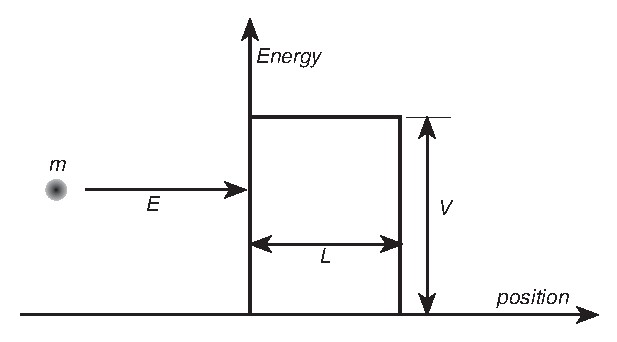
\includegraphics[]{QMBarrier}
% \epsfbox{Pix/QMBarrier.eps}
\end{center}
\caption{One Dimensional Barrier\label{QMBarrier:Fig}}
\end{figure}

This section demonstrates how an algebraic manipulation system might
be used to solve a problem in quantum mechanics that might arise in
practice, or at least in homework.  We wish to determine the
probability that a particle with mass $m$ and energy $E$ will pass
through the one dimension potential barrier given in
\figref{QMBarrier:Fig}.  This probability is called the {\em
transmission coefficient\/}.  We begin with the one dimensional, time
invariant Schr\"odinger equation:
\[
-{\hbar^2 \over 2 m} {d^2 \psi(x) \over dx^2} + V(x) \psi(x) = E
\psi(x).
\]
Here $\hbar = {h \over 2 \pi}$ where $h$ is Planck's constant.  The
mass of the particle is represented by $m$, and the energy by $E$.
The potential energy of the system is $V(x)$ and the wave function of
the particle is $\psi(x)$.

If the potential energy is constant we have
\[
{d^2 \psi(x) \over dx^2} + {2 m\,(E - V) \over \hbar^2} \psi(x) = 0.
\]
All solutions of this equation are linear combinations of two eigenfunctions
of the equations
\[
\psi(x) =  A e^{i \sqrt{2m\,(E - V)} x/ \hbar} + B e^{- i \sqrt{2m\,(E
- V)} x/ \hbar} 
\]
where $A$ and $B$ are arbitrary constants.  The first term in the sum gives
the probability amplitude of motion to the right (increasing $x$), while the
second term corresponds to motion to the left.  

We assume the height of the potential barrier is $V$ and that the
particle has energy $E$ with $E$ greater than $V$.
The barrier has has width $L$ and begins at $x=0$ and goes to
$x=L$.  We need to construct the wave function of a particle moving from
left to right and impinging on the barrier.  In each of the three regimes
$x<0$, $0<x<L$ and $L<x$, the potential is constant and thus the wave
function has the form given above.  We will use continuity conditions to
match the three wave functions at their boundaries.  This allows us to
determine the amplitudes of the wave functions.  We then compute the ratio
of the incoming amplitude and the outgoing amplitude.

We begin by setting two variables {\tt ALPHA} and {\tt BETA} to the wave
numbers of the particle outside the barrier and inside the barrier respectively
\begin{verbatim}
(C1) RADPRODEXPAND:FALSE$
\end{verbatim}
When {\tt RADPRODEXPAND} is set to true, expressions like $\sqrt{a b} /
\sqrt{a}$ will naturally simplify to $\sqrt{b}$ since the numerator will be
represented as $\sqrt{a} \sqrt{b}$.  We have set {\tt RADPRODEXPAND} to
false so that expressions like $\sqrt{2Em}$ will remain a single square
root as is conventional.
\begin{verbatim}
(C2) ALPHA:SQRT(2*M*E)/HBAR;
\end{verbatim}
\mdline{\sqrt{2Em} \over \hbar}{D2}
\begin{verbatim}
(C3) BETA:SQRT(2*M*(E-V))/HBAR;
\end{verbatim}
\mdline{\sqrt{2 m \,(E-V)} \over \hbar}{d3}
{\tt ALPHA} and {\tt BETA} are the two quantization constants that are
involved in the computation.  We use {\tt HBAR} to represent Planck's
constant.

\begin{verbatim}
(C4) A:1$

(C5) UL:A*%E^(%I*ALPHA*X)+B*%E^(-%I*ALPHA*X);
\end{verbatim}
\mdline{e^{i \sqrt{2Em} x / \hbar} + 
B e^{-{i \sqrt{2Em} x / \hbar}}}{D5}
This is the wave function to the left of the barrier.  Since the 
transmission coefficient is to be the ratio of $|A|^2$ and $|F|^2$, we
set {\tt A} to one here.  By eliminating this variable we reduce the number of
unknown variables to precisely the number of equations obtained by
fitting the pieces of the wave function together.
\begin{verbatim}
(C6) UC:C*%E^(%I*BETA*X)+D*%E^(-%I*BETA*X);
\end{verbatim}
\mdline{C e^{i \sqrt{2m\,(E-V)} x / \hbar}
+ D e^{-i \sqrt{2m\,(E-V)} x / \hbar}}{D6}
The wave function for the regime inside the potential barrier is similar,
but the wave number is different.
\begin{verbatim}
(C7) UR:F*%E^(%I*ALPHA*X);
\end{verbatim}
\mdline{F e^{i \sqrt{2Em} x / \hbar}}{D7}
Beyond the barrier we can assume that there is no reflection of the wave
at infinity.  Thus only one term is needed for the wave function.
\begin{verbatim}
(C8) UL-UC,X=0;
\end{verbatim}
\mdline{-D -C + B +1}{D8}
\begin{verbatim}
(C9) EQ1:%$

(C10) UC-UR,X=L$

(C11) EQ2:%$
\end{verbatim}
Since the wave function is continuous, the various pieces and their
derivatives must match up at the edges of the barrier.
\begin{verbatim}
(C12) EQ3:SUBSTITUTE(0,X,DIFF(UL-UC,X));
\end{verbatim}
\mdline{{i D \sqrt{2 m \, (E-V)} \over \hbar} -
{i C \sqrt{2 m \,(E-V)} \over \hbar} -
{i B \sqrt{2Em} \over \hbar}
+ {i \sqrt{2Em} \over \hbar}}{D12}
\begin{verbatim}
(C13) EQ4:SUBSTITUTE(L,X,DIFF(UC-UR,X))$
\end{verbatim}
These four expressions must be zero for the wave functions to be continuous
and have continuous derivatives.  The expressions are linear in the four
amplitudes, {\tt B}, {\tt C}, {\tt D} and {\tt F}.  Solving this system of
linear equations gives the value of {\tt F}.  We actually want 
the value of {\tt 1/F} since the transmission coefficient is the ratio of
those particles reflected by those which pass through the barrier.
\begin{verbatim}
(C14) SOLVE([EQ1,EQ2,EQ3,EQ4],[B,C,D,F])$

(C18) 1/F,%$
\end{verbatim}
This last quantity is too large to bother printing.  The probability
that particle will pass through the barrier is the magnitude of $F$
which can be determined by $F \overline{F}$, where $\overline{F}$ is the
complex conjugate of $F$.  {\Macsyma} does not have a  function that
computes the complex conjugate of an expression since the conjugate can
be determined by replacing all instances of $i$ in the expression by 
$-i$.  
\begin{verbatim}
(C19) SUBSTITUTE(-%I,%I,%)*%,RATSIMP;
\end{verbatim}
\mdline{e^{-{2 i L \sqrt{2Em-2mV} \over \hbar}}
\left( 
\begin{aligned}
    \displaystyle
    V^2 e^{4 i L \sqrt{2Em-2mV} / \hbar}\hfill\hfill\hfill\\
    \quad + \left( -2 V^2 + 16EV - 16E^2\right)e^{2 i L \sqrt{2Em-2mV} / \hbar}\\
    \quad +V^2
\end{aligned} \right)
\over 16EV - 16E^2}{D19}

The expression given in {\tt D19} is the transmission coefficient desired,
but is certainly not the expression normally given textbooks.  The next few
commands are devoted to simplifying {\tt D19}.  
\begin{verbatim}
(C20) (DEN:PART(%,2),NUM:PART(%,1))$

(C21) RATEXPAND(NUM);
\end{verbatim}
\mdline{
  \begin{aligned}
    V^2 e^{2 i L \sqrt{2Em -2mV} / \hbar}
      &+ V^2 e^{-{2 i L \sqrt{2Em -2mV} / \hbar}}\\
      &-2V^2 +16EV -16E^2
  \end{aligned}}{D21}
We would like to eliminate the complex exponentials.  We could apply
deMoivre's identity to {\tt D19} but a horrible mess of trigonometric
functions would result.  It would be quite difficult to cause {\Macsyma} to
produce the correct answer using that technique.  

The denominator already in roughly the form we would like.  To simplify some
of the steps that follow, we will deal with the numerator and denominators
separately. 
\begin{verbatim}
(C22) D21,DEMOIVRE,RATSIMP;
\end{verbatim}
\mdline{V^2 \left( 2 \cos {2 L \sqrt{2Em -2mV} \over \hbar} -2 \right)
+ 16 EV -16E^2}{D22}

The {\tt DEMOIVRE} command applies deMoivre's identity to {\tt D21}.  By
using {\tt RATSIMP} to simplify the expression the sine terms are caused to
cancel.  The coefficient of $V^2$ has the form $2 \cos 2 \theta - 2$.  We
next use the double angle formula to express {\tt D22} in terms of $\cos
\theta$.

\begin{verbatim}
(C23) ANS:EV(%/DEN,TRIGEXPAND);
\end{verbatim}
\mdline{
  \frac{
    \begin{aligned}
       V^2 \left( 2 \left( \cos^2 {L \sqrt{2Em -2mV} \over \hbar}
         - \sin^2 {L \sqrt{2Em -2mV} \over \hbar}\right) -2 \right)\qquad
         \hfill\\
       \hfill+ 16 EV -16E^2
    \end{aligned}}
    {16EV -16E^2}}{D23}
Unfortunately, {\Macsyma} uses the following double angle identity
\[
\cos 2\theta = \cos^2 \theta - \sin^2 \theta.
\]
By replacing $\cos^2 \theta$ by $1 - \sin^2 \theta$ the expression will be
reduced to a single trigonometric term.  The only problem is picking out
$\theta$.  

The {\tt PART} command in {\Macsyma} is used to out sub-expressions from
a larger expression.  Its first argument is the ``larger expression.''
The second argument says which part to return.  Thus given an
expression like
\[
w = x^2 + (2y - 1) x + 3
\]
{\tt PART($w$, 2)} is second argument to the top level sum, viz.,
$(2y-1) x$.  Successive {\tt PART} commands can be strung together by
additional selectors.  Thus {\tt PART($w$, 2, 1)} is $2y-1$ and so on.

For our problem, the following command will pick out the argument to the
cosine in $D23$.

\begin{verbatim}
(C24) PART(D23,1,1,2,1,2,1,1,1);
\end{verbatim} \mdline{{L \sqrt{2Em - 2mV} \over \hbar}}{D24}
\begin{verbatim}
(C25) SUBSTITUTE(1-SIN(D24)^2,COS(D24)^2,ANS);
\end{verbatim}
\mdline{{V^2\left(
2 \left(1 - 2\sin^2 {2L \sqrt{2Em-2mV} \over \hbar} \right)
 - 2\right)
+ 16EV - 16E^2 \over 16EV - 16E^2}}{D25}
{\Macsyma} likes to keep expressions as quotients of polynomials.  In this case
we would prefer to see the answer as $1 + <\hbox{quotient of polynomials}>$.
The following command does that. 
\begin{verbatim}
(C26) 1+FACTOR(RATSIMP(D25-1));
\end{verbatim}
\mdline{{\sin^2 \left({L \sqrt{2M (E - V)} \over \hbar}\right) V^2 \over 4E(E-V)} +1}{D26}
Thus the transmission coefficient for a particle impinging on a potential
barrier of height $V$ is
\[
1 + {\sin^2 {L \sqrt{2 m\,(E - V)} \over \hbar} V^2 \over 4 E \, (E - V)}.
\]
which is what we normally find in textbooks.

\section{Overview of the Algorithms and Capabilities}

As can be seen from these examples, algebraic manipulation systems can deal
directly with many of the quantities that arise in mathematics:
polynomials, rational functions, matrices and power series, for example.
Basic arithmetic operations with these types of objects can be implemented
relatively straightforwardly, however numerous performance complications
arise because of {\em intermediate expression swell\/}.  Arithmetic
operations with symbolic quantities tend to produce larger expressions from
smaller ones.  This distinguishes symbolic calculations from numeric ones
where numeric expressions tend not to grow in size.  Intermediate
expression swell occurs in a problem when the intermediate computations
swell to be much larger than the final answer.  A prime example of this
problem occurs when calculating polynomial GCD's.  These issues are
discussed in some detail in \chapref{Poly:Arith:Chap} and some approaches
to their solution are given in Chapters \ref{Interpolation:Chap} and
\ref{Hensel:Chap}. 

Symbolic systems are more likely to deal with infinite structures such as
ideals, lattices or power series, than numerical systems.  We want to perform
the same types of operations on these structures as on simpler structures.
In \chapref{Ideal:Arithmetic:Sec}.

There are certain additional operations that are possible with symbolic
quantities.  \Marginpar{orthogonal functions expansions, analysis of
singularities} 
Some operations that are impractical for numerical quantities
turn out to be quite cheap for symbolic expressions.  For instance,
there is no known polynomial time algorithm for factoring integers, and
more to the point it is quite hard in practice to factor integers.
However, there do exist polynomial time algorithms for factoring
polynomials, and in practice polynomials are relatively easy to
factor.\footnote{The distinction between practice and theory is made here
because the polynomial time algorithm is an $O(n^{12})$ algorithm, while
the exponential algorithms which are used in practice  usually only 
require $O(n^{3})$ operations.}

Another	aspect of symbolic computation is exact versus inexact computation.

Where there are similarities between numerical and symbolic calculations,
the introduction of symbolic parameters often allows one to examine a wide
variety of possibilities with a single computation.

Groups, Fields, Riemann surfaces, topological structures, etc as first
class objects.

Computations: arithmetic, solving systems of equations, approximation
techniques, etc.


Problems: simplification: definite canonical and normal simplifiers.




\section{Where Current Research is Heading}

With some exceptions the contents of this book are largely classical.
The algorithms discussed are solutions to the problems set out by
parents of the Computer Algebra field at the end of the 1960's.  Since
then, much has changed.  The massive increase in performance of computer
systems and their precipitative drop in price has changed many of the
premises upon which computer algebra research is based.



\part{Number Theory}
%$Id: euclids-alg.tex,v 1.1 1992/07/12 19:39:34 rz Exp rz $
\chapter{Euclid's Algorithm}
\label{Integer:GCD:Chap}

Among the mathematical problems we will investigate is the computation
of greatest common divisors, factoring into prime factors and finding
rational approximations.  These computations may be performed on a
variety of different mathematical quantities: polynomials, rational
integers, power series, differential operators, etc.  The most
familiar of these algebraic structures are the \keyi{natural numbers}:
$\mathbb{N} = \{1, 2, 3, \ldots\}$.  If we include zero and 
the negative integers we have $\Z$, the ring of \keyi{rational
integers}. The elements of $\Z$ are commonly called the  
\keyi{integers}, but we will use the term integer for more complex
algebraic structures. 
\addsymbol{$\mathbb N$}{The natural, or counting numbers, $1, 2, 3, \ldots$}
\addsymbol{$\Z$}{The ring of rational integers}
\addsymbol{$\Q$}{The field of rational numbers}

This chapter begins our study of mathematical algorithms with an
investigation of a variety of computations involving the rational
integers.  Later chapters discuss more elaborate algorithms that deal
with polynomials and other algebraic structures.  Interestingly, the
resolution of some of these problems for the rational integers can
lead to algorithms that make use of polynomials, thus making the whole
process somewhat circular.

\medskip
An integral part of our elementary education is learning to add and
multiply integers.  The hardware used in computers usually only
implements arithmetic operations for numbers of a specified length,
\ie, $32$-bit or $64$-bit integers.  In algebraic computation we often
use much larger integers; however, this is not because the answers are
so large.  Instead these large numbers arise in the middle of some
computation and then shrink towards the end.  This phenomenon is
called \keyi{intermediate expression swell}.

Detailed algorithms for integer arithmetic may be found in many texts,
\eg, {\Knuth} \cite{Knuth1997-tf} and {\Aho}, {\Hopcroft} and {\Ullman}
\cite{Aho1974-yy}. But implementing efficient variable
precision arithmetic algorithms is a very delicate process that raises
many issues not touched upon in these texts, such as register usage,
cache turbulence and pipeline stalls.  For instance, properly
implemented classical algorithms work very well for larger integers
than one might expect.  Because of all of these reasons, because
numerous variable precision integer packages are available and because
an increasing number of programming languages now provide variable
precision integers as one of their basic types, we do not discuss
these arithmetic algorithms.

\medskip
We begin with some basic definitions.  When a rational integer $m$ can
be written as a product of two other integers $p$ and $q$, $m = pq$,
then $p$ and $q$ are called {\em divisors}\index{divisor} of $m$ and
$m$ is said to be {\em divisible} by $p$ and
$q$.\index{divisibility!integer} We write $p \mid m$ to indicate that
$p$ divides $m$.  We indicate that $p$ does not divide $m$ by $p \nmid
m$.  The only rational integers that have multiplicative inverses are
$1$ and $-1$.  Because they have multiplicative inverses they are
called {\em units}.\index{unit, of a ring} Two integers whose ratio is
a unit are said to be \keyi{associates}.  For simplicity we will
ignore associates when enumerating the divisors of an integer.  Thus
every non-unit has at least two divisors, $1$ and itself (up to
associates).  An integer that has only these two ``trivial''
divisors\index{trial division} is called a \keyi{prime}.  All other
non-units are called \keyi{composite}.
\addsymbol{$p \mid m$}{$p$ divides $m$}
\addsymbol{$p \nmid m$}{$p$ does not divide $m$}

A presentation of a positive integer $N$ as a product of positive
integers, $N = m_1 \cdots m_k$, is called a \keyi{factorization} of
$N$.  A factorization of an integer is said to be {\em
complete}\index{factorization!complete} if each of the $m_i$ is a
prime or a power of a prime.  Unless otherwise noted, all
factorizations are complete.  We usually write such factorizations as
$N= p_1^{e_1} \cdots p_k^{e_k}$.  According to the
\key{fundamental theorem of arithmetic} the factorization of a
rational integer is unique.

The factoring problem for an integer $N$ is, at the moment, very
difficult.  Trying all possible divisors takes time $O(\sqrt{N})$.
Very roughly, the best known algorithms take time $O(\exp(\sqrt{\log
N}))$, which, though much better, is not near what would be expected
of a polynomial time algorithm: $O(\log^k N)$.  Interestingly, the
time required to factor a polynomial of degree $n$ is only about $O(n^5)$.

An integer $d$ that divides both $m$ and $n$ is called a \keyi{common
divisor} of $m$ and $n$.  The number $m/d$ is called the
\keyi{cofactor} of $m$ with respect to $d$.  The largest common
divisor of two integers is called a \keyi{greatest common divisor}
({\sc gcd}).  If the greatest common divisor of two integers is $1$,
then we say they are {\em relatively prime\/}.\index{relatively prime}
When dealing with rational numbers, more time is probably spent
computing the {\sc gcd} of integers than any operation other than
addition and multiplication.  When using rational functions, it is not
unusual for the time spent computing polynomial {\sc gcd}s to dominate
all other arithmetic operations.  \sectref{Integer:Euclidean:Sec}
discusses Euclid's algorithm for computing the {\sc gcd} of two
integers.  Euclid's algorithm provides an entr\'e to many facets of
elementary number theory.  The other sections of this chapter
illustrate several of these ideas.  Later chapters delve into each of
the issues raised in more detail.

\section{Euclidean Algorithm}
\label{Integer:Euclidean:Sec}

\index{Euclidean algorithm|(}
The {\em Euclidean algorithm} for computing the {\sc gcd} of two
integers has been known at least from the time of \key{Euclid}
\cite{Fritz1945-sw}, who called it ``\key{anthyparesis}.''  Most
likely, it is the oldest mathematical algorithm in existence.  The
principles underlying the Euclidean algorithm are fundamental to the
solution of many problems in mathematics ranging from diophantine
approximation to elimination.  Because of its importance, and because
it is the first algorithm we consider, we derive Euclid's algorithm in
some detail.

Let $m > n$ be two positive rational integers.  Denote by $d$ some
common divisor of $m$ and $n$.  $d$ also divides, $m+n$ and $m-n$.  In
fact, $d$ divides every number of the form $am - bn$, where $a$ and
$b$ are rational integers.  Denote by $M$ the set of all such numbers
\[
M = \{ am - bn \mid a,b \in \Z\}.
\]
Since every common divisor of $m$ and $n$ divides every element of
$M$, each is also a multiple of the greatest common divisor of $m$ and
$n$.  Thus the smallest positive element of $M$ is the {\sc gcd} of $m$ and
$n$.

To make this an algorithm, we use a simple recursive technique that
converts a pair of elements in $M$ into a pair of smaller elements.
This process terminates with the pair $0$ and the {\sc gcd} of $m$ and
$n$.  The simplest approach is to replace the pair $(m,n)$ by
$(m-n,n)$, and then $(m-2n, n)$, and so on until $m-kn < n$.  At this
point the two values are interchanged and the new pair is $(n, m-kn)$.

\index{remainder}
All of the subtraction operations prior to an interchange of $m-n$ and
$n$ can be collapsed into a single division:
\begin{equation}
m = q n + r.\qquad\qquad 0 \le r < n 
\label{Remainder:Eq}
\end{equation}
In this case, $r$ is called the {\it remainder} of $m$ divided by $n$.
(This definition works both for positive and negative values of $m$
and $n$.)  Now let $n_1 = m$ and $n_2 = n$.  The sequence of
divisions and remainders used in the {\sc gcd} algorithm would look like:
\begin{equation} \label{Int:RemainderSeq:Eq}
  \begin{aligned}
   n_1 &= q_1 n_2 + n_3\\
   n_2&=q_2 n_3 + n_4\\
     &\vdots\\
   n_k& = q_k n_{k+1} + 0
  \end{aligned}
\end{equation}
This sequence of operations is called a \keyi{remainder sequence}, and
its use to compute the {\sc gcd} of two numbers is called Euclid's
algorithm.  \figref{Int:Euclid:Alg:Fig} illustrates the computation of
the {\sc gcd} of $15027133$ and $8562227$.  In this case the {\sc
gcd} is $163$ which we write as 
\[
(10527133, 8562227) = 163.
\]

\begin{figure}
\[
\begin{aligned}
  15027133 &= 1 \cdot 8562227 + 6464906\\
  8562227  &= 1 \cdot 6464906 + 2097321\\
  6464906  &= 3 \cdot 2097321 + 172943\\
  2097321  &= 12 \cdot 172943  + 22005\\
  172943   &= 7 \cdot 22005   + 18908\\
  22005    &= 1 \cdot 18908   + 3097\\
  18908    &= 6 \cdot 3097    + 326\\
  3097     &= 9 \cdot 326     + 163\\
  326      &= 2 \cdot 163     + 0
\end{aligned}
\]
\caption{Euclidean algorithm for two integers\label{Int:Euclid:Alg:Fig}}
\end{figure}


The following recursive function gives a direct implementation of the
Euclidean algorithm for two positive integers, based on the discussion
of the previous few paragraphs.

\begin{lstlisting}[language=Python]
def IntGcd(m, n) -> int:
  if m < n:
    return IntGcd(n, m)
  elif n == 0:
    return m
  else:
    return IntGcd(n, m % n)
\end{lstlisting}

The bulk of the work is performed in the remainder calculation.  For
some machines, it may be substantially cheaper to compute something
slightly larger than the remainder.  For instance, the first several
bits of $m$ and $n$ allow us to estimate the size and first few bits
of the quotient of $m$ and $n$ quickly.  Using this value, something
close to the remainder can be computed quite quickly.  Other
algorithms are described in Section 4.5.2 of {\Knuth} \cite{Knuth1997-tf}.

The second question we have about every algorithm is: How fast is it?
(The first question is whether or not the algorithm gives the correct
answer!)  To answer this question we bound the number of remainder
steps required 
to compute the {\sc gcd} of two integers.  Denote by $F(N)$ the
maximum number of 
remainder steps required to compute the {\sc gcd} of two positive
numbers less than $N$.

Assume $u > v$ are two positive integers without a common factor, each
larger than $N$ and chosen such that the quotients in their remainder
sequence are all $1$.  Thus, the {\sc gcd} of two integers smaller
than $N$ cannot take any more steps than the number required by $u$
and $v$.  The pair of integers $u+v$ and $u$ also has a remainder
sequence where each $q_i$ is $1$, and the remainder sequence for
$(u+v, u)$ is one step longer than that for $(u, v)$.  The sequence
$v, u, u+v, 2u+v,
\ldots$, can be continued as far as one would like.

To obtain a bound on the number of steps in a {\sc gcd} algorithm, we need
to be able to compute the growth rate of the terms of this sequence.
A crude bound can be determined by the following simple reasoning.

Assume that when the Euclidean algorithm is applied to two integers
$F$ and $G$, $F > G$, the remainder sequence is as long as possible.
For this to be the case, the quotient of $F$ divided by $G$ should be
$1$.  Denote the remainder by $H$.  For $F$ and $G$ to have a long
remainder sequence $G$ and $H$ must also.  Thus the quotient of $G$
divided by $H$ should also be one.  This suggests that we should
consider the sequence of numbers $f_i$ satisfying the 
recurrence
\begin{equation}
\label{Fibonacci:Eq}
f_{i+1} = f_i + f_{i-1},
\end{equation}
where we can take the basis of the \keyi{difference equation} to be $f_{1} =
f_{2} = 1$.  $f_i$ has a remainder sequence of length $i-1$ when
divided by $f_{i-1}$ and no smaller number can have a remainder
sequence so long.\label{Fibonacci:Remainder:Sequence}

Since the integer quotient of $f_{i}$ divided by $f_{i-1}$ is $1$,
$f_{i} < 2 f_{i-1}$.  This allows us to bound $f_{i+1}$ above and
below as follows:
\[
3 f_{i-1} > f_{i+1} > \frac{3}{2} f_{i},
\quad\mbox{or}\quad
c_1\left(\sqrt{3}\right)^i > f_{i+1} > c_2 (\frac{3}{2})^{i}.
\]
Consequently,
\[
F(N) = O(\log N).
\]

We can improve the constants in the estimates for $f_{i+1}$ above with
only a bit more work.  Assume that for large $i$ the ratio between
$f_{i+1}$ and $f_i$ tends to a constant, $\phi$.  Then for sufficiently
large $n$ we have 
\[
\phi = \frac{f_{n+1}}{f_n} = \frac{f_n + f_{n-1}}{f_n} = 1 + \frac{1}{\phi}.
\]
This gives a quadratic equation for $\phi$, $x^2 - x - 1=0$, whose
only positive solution is
\[
\phi = \frac{1 + \sqrt{5}}{2} \approx 1.618033988749894.
\]
So we expect $f_i = c_1 \phi^i$.  
Notice that this lies between the bounds given above of $\sqrt{3} =
1.732$ and $3/2 = 1.5$.  

We can go further and determine an exact formula for $f_i$.  Notice that if
$\alpha$ is a zero of $x^{2} -x -1$ then $\alpha^{i}$ will satisfy
\eqnref{Fibonacci:Eq}: 
\[
f_{i+1} - f_{i} - f_{i-1} = \alpha^{i+1} - \alpha^{i} - \alpha^{i-1}
 = \alpha^{i-1} ( \alpha^{2} - \alpha -1) = 0.
\]
Since \eqnref{Fibonacci:Eq} is a linear \key{difference equation},
linear combinations of the solutions of \eqnref{Fibonacci:Eq} are also
solutions.  The negative solution of the quadratic equation is $1-\phi
= -1/\phi$. Consequently,
\[
f_i = c_1 \phi^i + c_2 (-\phi)^{-i},
\]
where, as with ordinary differential equations, $c_1$ and $c_2$ are
determined by the ``initial conditions.''  Using $i = 1$ and $i=2$ we
have
\[
\begin{aligned}
  c_1 \phi - c_2 \phi^{-1} &= f_{1} = 1,\\
  c_1 \phi^2 + c_2 \phi^{-2}&= f_{2} = 1,
\end{aligned}
\]
whose solution is
\[
\begin{aligned}
  c_1 &= \frac{\phi +1}{\phi^3 +\phi} = \frac{1}{\sqrt{5}},\\
  c_2&=\frac{\phi^2 - \phi^3}{\phi^2 + 1} = - \frac{1}{\sqrt{5}}
\end{aligned}
\]
Thus,
\[
f_i = 
\frac{1}{\sqrt{5}} \left[
\left(\frac{1 + \sqrt{5}}{2}\right)^i -
        \left(\frac{1 - \sqrt{5}}{2}\right)^i \right]
\]

This sequence of numbers is called the \keyi{Fibonacci numbers}.  They
were first mentioned by {\Fibonacci} \cite[pages 283--285]{Pisano1857-nc}
and have important applications in number theory, complexity theory
and other fields.

Since the negative solution of the quadratic equation has absolute
value less than $1$, for large $i$, the Fibonacci numbers can be
approximated by
\[
f_i = \frac{\phi^i}{\sqrt{5}}
\]
for large $i$. Consequently,
\[
F(N) \approx \frac{\log \sqrt{5} N}{\log \phi} = \log_{\phi} \sqrt{5} N.
\]
These results were first demonstrated  by {\Lame} in 1844 \cite{Lame1844-wm}.

The techniques used to solve this simple \key{difference equation} are
similar to those used to solve constant coefficient linear
differential equations.  More complicated difference equations often
occur when analyzing algorithms and in other problems.  Obtaining
closed form and asymptotic solutions of difference equations is
somewhat similar to the corresponding problems for differential
equations where symbolic techniques have had dramatic success in
recent years.  The field of difference equation problems has not been
as closely examined and remains a fertile area for future research.

\index{Euclidean algorithm|)}

\section{Diophantine Approximations}
\label{Euclid:DA:Sec}

Returning to the original problem, assume we are interested in
computing the {\sc gcd} of $n_1$ and $n_2$.  For simplicity we assume
the {\sc gcd} is $1$.  Define $M$ to be the set
\[
M = \{ n_1 X - n_2 Y \mid X, Y \in \Z \}.
\]
The {\sc gcd} of $n_1$ and $n_2$ is the smallest positive element of $M$.
In other words, we want to find the smallest non-trivial value of the
binary form $|n_1 X - n_2 Y|$.  Another way to say this, is that we want
to find the best possible rational number approximation to $n_1/n_2$:
\[
\left|\frac{n_1}{n_2} - \frac{Y}{X}\right| \le \frac{1}{n_2 X} < \frac{1}{X^2}.
\]

Looking closely at the remainder sequence\index{remainder
sequence!integer} \eqnref{Int:RemainderSeq:Eq}, we can see how to find
the candidate solutions $X$ and $Y$.  By isolating the remainder terms
on one side of the equation we have
\[
  \begin{aligned}
    n_1 - q_1 n_2 &= n_3,\\
    n_2 - q_2 n_3 &= n_4,\\
     &\vdots\\
    n_{k-1} - q_{k-1} n_{k} &= 1.
  \end{aligned}
\]
We can substitute the value of $n_3$ given in the first equation into
the second equation, to get a relationship between $n_1$, $n_2$ and
$n_4$:
\begin{equation}\label{Euclid:Int:D:Eq}
-q_2 n_1 + (q_1 q_2 + 1) n_2 = n_4.
\end{equation}
Writing this relation in the form of an approximation to $n_1/n_2$  gives
\[
\left|\frac{n_1}{n_2} - \frac{q_1 q_2 + 1}{q_2}\right| 
= \frac{n_4}{n_2 q_2}.
\]

Using \eqnref{Euclid:Int:D:Eq}, and $n_3 = n_1 - q_1 n_2$, we can
obtain a relationship between $n_1$, $n_2$ and $n_5$:
\[
\left|\frac{n_1}{n_2} - \frac{q_1 q_2 q_3 + q_1 + q_3}{q_2 q_3 +1 }\right| 
= \frac{n_5}{n_2 (q_2 q_3 +1)}.
\]
Notice that 
\[
\frac{n_4}{n_2 q_2} > \frac{n_5}{n_2 (q_2 q_3 +1)},
\]
so the Euclidean algorithm is actually producing increasingly accurate
approximations to $n_1/n_2$.

When this process is taken to its logical conclusion, one obtains two
polynomials $X$ and $Y$ in the quotients $q_1, \ldots, q_{k-1}$ such
that
\[
 n_1 X - n_2 Y = 1,
\]
since $n_1$ and $n_2$ are relatively prime.  $Y/X$ is a quite
good approximation to $n_1/n_2$:
\[
\left|\frac{n_1}{n_2} - \frac{Y}{X}\right| = \frac{1}{n_2 X} 
   <  \frac{1}{X^2}.
\]
Observe that fractions with a denominator of $X$ can only approximate
real numbers to an accuracy of $1/2X$.  

The problem just studied can be phrased as trying to minimize the
value of the form $X r - Y$, where $r$ is a rational number.  There are
many interesting generalizations.  If $r$ is replaced by an algebraic
number, then it turns out that there are an infinite number of
``exceptionally'' good approximations to $r$ if $r$ is the solution of
a quadratic equation with integer coefficients, but only a finite
number of such solutions when $r$ is of higher degree.

It is also interesting to consider multiple approximations.  Given
real numbers $\alpha_1, \alpha_2, \ldots, \alpha_k$, we would like to
find integers that minimize the linear form:
\[
\left|X_0 + X_1 \alpha_1 + X_2 \alpha_2 + \cdots + X_k \alpha_k \right|.
\]
This type of problem is discussed in \chapref{Lattice:Chap} and can be
used to develop theoretically efficient algorithms for factoring
polynomials.

\section{Continued Fractions}
\label{Euclid:CF:Sec}

The approximation ideas of the previous section can be further developed
by rewriting the remainder sequence \eqnref{Int:RemainderSeq:Eq} in terms
of fractions.  This gives:
\begin{equation}\label{Euclid:CF:Eq}
  \begin{aligned}
    \frac{n_1}{n_2} &= q_1 + \frac{n_3}{n_2},\\
    \frac{n_2}{n_3} &= q_2 + \frac{n_4}{n_3},\\
     &\vdots\\
    \frac{n_{k-1}}{n_k} &=  q_{k-1} + \frac{1}{n_k}.
  \end{aligned}
\end{equation}
Replacing $n_3/n_2$ by the value in the second of these equations,
and continuing we have:
\[
\begin{aligned}
\frac{n_1}{n_2} &= q_1 + \frac{n_3}{n_2} = 
 q_1 + \frac{1}{\displaystyle q_2 + \frac{n_4}{n_3}}, \\
& = \frac{n_1}{n_2} = q_1 + \frac{1}{\displaystyle q_2 + 
    \frac{1}{\displaystyle q_3 + 1 \frac{1}{\displaystyle q_4 +
\ddots}}}.
\end{aligned}
\]
This strange way of writing the fraction $n_1/n_2$ is called a
\keyi{continued fraction}.   The $q_i$ that appear in the continued
fraction are called the {\em partial quotients}.\index{partial
quotient} From
\eqnref{Euclid:CF:Eq} and using the fact that $n_1 > n_2 > n_3 >
\cdots$ we see that  $q_i$ is the integer part of $n_i/n_{i+1}$.

Truncating the continued fraction and clearing the denominators:
\[
\begin{aligned}
q_1 + \frac{1}{q_2} & = \frac{q_1 q_2 + 1}{q_2}, \\
q_1 + \frac{1}{\displaystyle q_2 + 
    \frac{1}{\displaystyle q_3}} & = 
  \frac{q_1 q_2 q_3 + q_1 + q_3}{q_2 q_3 + 1}.
\end{aligned}
\]
Notice that these are the ``exceptionally'' good approximations to
$n_1/n_2$ discovered earlier.  This property is one of the reasons for
the interest in continued fractions.  \chapref{CF:Chap} discusses some
of the properties of continued fractions in more detail and how to
perform calculations with them.

\section{Diophantine Equations}
\label{Euclid:DE:Sec}

If we are only interested in the integral (or perhaps rational)
solutions of a polynomial equation (or system of equations), then we
call the problem a {\em diophantine} problem.\index{diophantine
equation} The simplest diophantine equation has already appeared.  To
compute the best rational approximation of $n_1/n_2$ we were looking
for integers $X$ and $Y$ such that
\begin{equation}\label{Euclid:Approx:Eq}
n_1 X - n_2 Y = 1.
\end{equation}
This is a  diophantine equation in $X$ and $Y$ since only elements of
$\Z$ are of interest in its solution.

This equation does have an infinite number of solutions, however.  Let
$x$ and $y$ be a solution of \eqnref{Euclid:Approx:Eq}.  Then $x+n_2
t$ and $y+ n_1 t$ is also a solution for integral values of $t$.  Thus
there are a countable number of solutions to \eqnref{Euclid:Approx:Eq}
as a diophantine problem.

Diophantine equations arise in a number of problems.  We give two more
examples here.  An integral \keyi{Pythagorean triangle} is a right
triangle (in Euclidean space) whose sides are each rational integers.
By the Pythagorean theorem their sides are zeroes of
\[
x^2 + y^2 = z^2,
\]
where $z$ is the length of the hypotenuse.  This equation involves three
unknown variables and is quadratic, not linear.  As an equation over
the reals, it has a continuously infinite number of solutions.  As a
diophantine equation, it has only a countably infinite number of
solutions, which can be parameterized as 
\begin{equation}\label{PythagEq:Soln:Eq}
x = r^2 - s^2, \quad y = 2rs, \quad z = r^2 + s^2.
\end{equation}
We leave the proof of this to the reader.  

What integers can arise as the sides of a Pythagorean triangle?  Any
even integer, \eg, $2k$ can be a side:
\[
(k^2 - 1 , 2k, k^2+1).
\]
Odd integers can also be sides, since every odd number is the difference
of two squares, $2k+1 = (k+1)^2 - k^2$.  Thus,
\[
(2k+1, k(k+1), 2k^2+2k +1)
\]
is a Pythagorean triple.

A more challenging question is: Which rational integers can be the
{\em area} of a Pythagorean triangle?  If the sides of the triangle
are restricted to be rational integers then the area must be of the
form $rs(r^2-s^2)$.  However, it is more interesting to consider
triangles whose sides are rational numbers and whose area is an
integer.\Marginpar{Need to give an example here and give a bit more detail.}

Pythagorian triangles with rational sides can be determined by
allowing $r$ and $s$ to be rational in \eqnref{PythagEq:Soln:Eq}.  (Do
all Pythagorean triangles with rational sides arise in this fashion?)

The integer $n$ is the area of a Pythagorean triangle if $xy = 2n$ and
$x^2 +y^2 = z^2$.  Eliminating $y$ we have
\[
x^2 + \left(\frac{2n}{x}\right)^2 = z^2 \Longrightarrow x^4 + 4n^2 =
(xz)^2.
\]
Rewriting this slightly, we want to know if there exist rational
numbers $u$ and $v$ such that
\begin{equation}\label{Euclid:Cong:Eq}
u^2 = v^4 + 4n^2.
\end{equation}
This is a far harder diophantine equation to solve.  In this case
there are only a finite number of solutions and proving this is quite
difficult.  To do so requires techniques of {\em elliptic
curves}.\index{elliptic curve} This problem is beyond the grasp of the
techniques discussed in this book.  A nice presentation of the
mathematics relevant to this problem and its solution is given in
{\Koblitz}'s book \cite{Koblitz2012-wq}.

\section*{Notes}

\small

If $F$ is a purely algebraic extension of the rational numbers, $\Q$,
then every element $\alpha \in F$ is the zero of a polynomial with
coefficients in $\Z$.  If $\alpha$ is the zero of a polynomial whose
\key{leading coefficient} is $1$ then $\alpha$ is said to be an
\keyi{integral element} of $F$.  The ring of integral elements of $F$
is called the \keyi{ring of integers} of $F$.  The ring of integers of
$\Q[\sqrt{-1}]$ is $\Z[\sqrt{-1}]$ and the elements of $\Z[\sqrt{-1}]$
are called \keyi{Gaussian integers}.  The ring of integers of
$\Q[\sqrt{5}]$ is $\Z[(1+\sqrt{5})/2]$.

The integral elements of $\Q$ are the elements of $\Z$.  Throughout
this book we use the term \keyi{rational integer} instead of just {\em
integer} to be more precise.

\normalsize

%$Id: cont-frac.tex,v 1.2 1992/05/10 19:34:57 rz Exp rz $
\chapter{Continued Fractions} 
\label{CF:Chap}

\def\Ddots{\mbox{\raisebox{-2ex}{$\ddots$}}}
\index{continued fraction|(}


By a \keyi{continued fraction} we mean an expression of the form
\[
a_0 + \frac{b_1}{\displaystyle a_1 + \frac{b_2}{\displaystyle a_2 + \Ddots}}\ .
\]
When this expression is finite, it represents a rational number. The
infinite form of of the continued fraction is defined to be the 
limiting value of the sequence 
\[
a_0, \quad a_0 + \frac{b_1}{a_1}, \quad 
a_0 + \frac{b_1}{\displaystyle a_1 + \frac{b_2}{a_2}}, \quad \ldots,
\]
if the limit exists.  Assume the limit does exist, and denote it by
$\alpha$.  The elements of this sequence are called the  
{\em continued fraction convergents}\index{convergents!of a continued
fraction} of $\alpha$.  When the $b_i$ are equal to 1, the 
elements of the above sequence are quite good approximations to
$\alpha$ and, in a certain sense, all of the ``best'' approximations
to $\alpha$ are elements of the sequence.

The major goal of this chapter is to make these concepts precise and
to provide algorithms for determining these convergents efficiently.
These results will provide efficient algorithms for solving certain
diophantine problems.

\section{Basics}
\label{CF:Basics:Sec}

We consider only continued fractions where the numerators are $1$,
\ie, fractions of the form
\[
a_0 + \frac{1}{\displaystyle a_1 + \frac{1}{a_2 + \Ddots}},
\]
and where the $a_i$ are positive integers.  A continued fraction of
this form is called a {\em simple continued
fraction\/}\index{continued fraction!simple}.  To simplify the
notation, simple continued fractions are written as
\[
a_0 + \frac{1}{\displaystyle a_1 + \frac{1}{a_2 + \Ddots}}
    = [a_0,a_1, a_2, \ldots].
\]
The $a_i$ are called the {\em partial quotients}\index{partial
quotient} of the continued fraction.  The $n$-th {\em
convergent}\index{continued fraction!convergent} of a continued
fraction is defined as:
\[
\frac{P_n}{Q_n} = [a_0, a_1, \ldots, a_n].
\]
\addsymbol{$[a_0, a_1, \ldots]$}{Continued fractions with partial
quotients $a_i$}

Let $\alpha = [a_0, a_1, \ldots]$, where only the finite
series is well defined at this time.  Notice that the expression
\[
\frac{1}{\displaystyle a_1 + \frac{1}{a_2  + \Ddots}}
\]
is always positive and less than $1$.  Therefore, $a_0$ is the
\key{integer part} of $\alpha$, which we denote by 
$\lfloor \alpha \rfloor$.  (We use $\lceil \alpha \rceil$ to denote
the smallest integer greater than or equal to $\alpha$.)  The second
partial quotient is
\[
a_1 = \left\lfloor \frac{1}{\alpha - a_0} \right \rfloor = \lfloor
\alpha_1 \rfloor,
\]
and so on. 
\addsymbol{$\lfloor \alpha \rfloor$}{The greatest integer less than or
equal to $\alpha$}
\addsymbol{$\lceil \alpha \rceil$}{The smallest greatest integer
greater than or equal to $\alpha$}


If $\alpha$ is a rational number, this process will terminate with a
finite simple continued fraction of the form
\[
\alpha = [a_0, a_1, \ldots, a_n ] = [a_0, a_1, \ldots, a_n -1, 1],
\]
where the last step is a reflection of the identity
\[
k = (k-1) + \frac{1}{1}.
\]
Any finite continued fraction represents a rational number, so 
irrational numbers have infinite continued fractions expansions.
These expansions are unique, the proof of which we leave to the
reader.  We summarize these results in the following proposition.

\begin{proposition}
Let the simple continued fraction expansion of $\alpha$ be
\[
\alpha = [a_0, a_1, \ldots, a_k, \ldots ].
\]
If $\alpha$ is irrational this expansion will not terminate and it is
unique.  If $\alpha$ is rational, then it has precisely two simple
continued fraction expansions and they are related as follows
\[
\alpha = [a_0, a_1, \ldots, a_n] = [a_0, a_1, \ldots, a_n-1, 1].
\]
Thus a rational number has a unique continued fraction expansion with
an even number of partial quotients and a unique continued fraction
expansion with an odd number of partial quotients.

\end{proposition}

\bigskip
A good example of the types of approximations produced by continued
fractions  is given by $\pi$.  Apply the procedure given above
to $\pi$ (using a calculator, for instance) gives
\[
\begin{array}{rlc}
\alpha = \pi &= 3.141592653589793\ldots & a_0 = 3 \\
\alpha_1 = (\pi - 3)^{-1} &= 7.062513305931052\ldots 
   & a_1 = 7 \\
\alpha_2 = (\alpha_1 - 7)^{-1} &= 15.996594406684104\ldots 
   & a_2 = 15 \\
\alpha_3 = (\alpha_2 - 15)^{-1} &= 1.0034172310150003\ldots 
   & a_3 = 1 \\
\vdots  & \vdots 
\end{array}
\]
When computed with enough precision, we discover that
\[
\pi = [3,7,15,1,292,1,1,1,2,1,3,1,14,2,1,1,2,2,2,2,1,84, \ldots].
\]
The resulting convergents are 
\[
3,\quad \frac{22}{7},\quad \frac{333}{106},\quad \frac{355}{113},
  \quad \frac{103993}{33102}.
\]
The first convergent is the Biblical value for $\pi$, the second is
the value often used in hand calculations prior to the appearance of
the calculator, and the fourth is well known as being an exceptionally
accurate value for a fraction with such a small denominator---its
error is less that $10^{-6}$.  In general, the convergent before a
particularly large partial quotient will be especially
accurate.\index{$\pi$, biblical value}

The numerical values of the continued fraction convergents of $\pi$ given
above are
\[
3.0,\quad 3.142857, \quad 3.141509, \quad 3.141593, \quad 3.1415926.
\]
Notice that these approximations are alternately larger and then smaller
than $\pi$.  This is true of all simple continued fractions, as we
shall prove in \propref{CF:Convergence:Prop}.

\bigskip

To simplify some of the notation that follows it is convenient to add two
extra convergents to the set derivable from the continued fraction.  The value
of a simple continued fraction is always less than $\infty$ and greater than
0.  We can preserve the alternating behavior of the convergents by letting
the $-1${\st} convergent be $1/0$ and the $-2$-nd be $0/1$.

The first few convergents of a continued fraction
$[a_0, a_1, a_2, \ldots]$ are thus
\[
\begin{array}{c|ccccc}
    n & -2 & -1 & 0 & 1 & 2 \\ \hline\noalign{\vspace{2pt}}
    \displaystyle\frac{P_n}{Q_n} & \displaystyle\frac{0}{1}& \displaystyle\frac{1}{0}&
    \displaystyle\frac{a_0}{1}& \displaystyle\frac{a_0 a_1 + 1}{a_1} &
    \displaystyle\frac{a_0 a_1 a_2 + a_2 + a_0}{a_1 a_2 + 1}
\end{array}
\]
These examples suggest that the convergents of a continued fraction
satisfy the following simple pair of recurrence relations:
\begin{equation}
\label{CFRecurrence:Eq}
 \begin{aligned}
  P_{n+1} &= a_{n+1} P_n + P_{n-1},\\
  Q_{n+1} &= a_{n+1} Q_n + Q_{n-1}.
 \end{aligned}
\end{equation}
This is in fact the case and will be shown in
\propref{CF:Recurrence:Prop}. First, we show that sequences that
satisfy \eqnref{CFRecurrence:Eq} satisfy certain identities.

\begin{proposition}\label{CF:Identities:Prop}
If $P_k/Q_k$ satisfy the relations \eqnref{CFRecurrence:Eq} then 
\begin{align}
  P_n Q_{n-1} - P_{n-1} Q_n &= (-1)^{n-1}, \label{CFUnitIdentity:Eq} \\
  P_n Q_{n-2} - P_{n-2} Q_n &= a_n(-1)^{n}. \label{CF:2Dif:Identity:Eq} 
\end{align}
\end{proposition}

\begin{proof}
The first identity is easily shown using induction.  Equation
\eqnref{CFUnitIdentity:Eq} is true for $n= 0, 1$.  Assuming
\eqnref{CFUnitIdentity:Eq} is true for $n = k$ we have for $n = k+1$: 
\[
\begin{aligned}
  P_{k+1} Q_k - P_k Q_{k+1}
    & =(a_{k+1} P_k + P_{k-1}) Q_k - P_k \,(a_{k+1} Q_k + Q_{k-1})\\
    &= P_{k-1} Q_k - P_k Q_{k-1} \\
    &= (-1)^{k}
\end{aligned}
\]

Rewriting \eqnref{CFUnitIdentity:Eq} in terms of the convergents gives
\[
\frac{P_n}{Q_n} - \frac{P_{n-1}}{Q_{n-1}} = \frac{(-1)^{n-1}}{Q_{n-1}
Q_n}.
\]
Consequently,
\[
\begin{aligned}
\frac{P_n}{Q_n} - \frac{P_{n-2}}{Q_{n-2}} &= 
 \frac{P_n}{Q_n} - \frac{P_{n-1}}{Q_{n-1}} + 
 \frac{P_{n-1}}{Q_{n-1}} - \frac{P_{n-2}}{Q_{n-2}}, \\
& = \frac{(-1)^{n-1}}{Q_{n-1}Q_n} + \frac{(-1)^{n}}{Q_{n-2}Q_{n-1}}
  = \frac{(-1)^{n}}{Q_{n-2} Q_n}\left[ \frac{Q_n - Q_{n-2}}{Q_{n-1}}
     \right], \\
 & = a_n \frac{(-1)^n}{Q_{n-2} Q_n}.
\end{aligned}\]
Clearing denominators gives \eqnref{CF:2Dif:Identity:Eq}.
\end{proof}

Notice that $P_n$ and $Q_n$ are relatively prime, since any common
divisor they shared would also divide $-1$.  Now we demonstrate that the
$P_k/Q_k$, as defined by \eqnref{CFRecurrence:Eq}, are the convergents
of the continued fraction of their limit.

\begin{proposition}\label{CF:Recurrence:Prop}
If $P_k/Q_k = [a_0, a_1, \ldots, a_k]$, then $P_n$ and $Q_n$ satisfy
\eqnref{CFRecurrence:Eq} when each of the terms are defined.
Furthermore, if the $a_i$ are all positive then $P_i > P_j$ and $Q_i >
Q_j$ if and only if $i > j$.
\end{proposition}

\begin{proof}
This identity is easily verified for small $n$.  The other cases are
handled by induction.  Assume the identity is true for $n=k$.  From
the definition of a continued fraction it is clear that
\[
[a_0, a_1, \ldots, a_{k+1}] =
[a_0, a_1, \ldots, a_k + \frac{1}{a_{k+1}}]
\]
Consequently,
\[
\begin{aligned}
  \frac{P_{k+2}}{Q_{k+2}} &=
      \frac{\left(\displaystyle a_{k+1} + \frac{1}{a_{k+2}}\right) P_{k} + P_{k-1}}{\left(\displaystyle a_{k+1} + \frac{1}{a_{k+2}}\right) Q_{k} + Q_{k-1}},\\
    & = \frac{a_{k+1} a_{k+2} P_k + P_k + a_{k+2} P_{k-1}}{
              a_{k+1} a_{k+2} Q_k + Q_k + a_{k+2} Q_{k-1} },\\
    & = \frac{a_{k+2} P_{k+1} + P_k}{a_{k+2} Q_{k+1} + Q_k}.
\end{aligned}
\]
Since, $P_{k+2}$ and $Q_{k+2}$ are relatively prime we can equate the
numerators and denominators of this equation to get the identities.

The final statement in the proposition follows immediately from
\eqnref{CFRecurrence:Eq}.  
\end{proof}

The recurrence relations \eqnref{CFRecurrence:Eq} make computing the
convergents of a continued fraction very easy, as shown in the
computation of the convergents of $\pi$ in the tableau below.
\[
\begin{array}{|c|c|c|c|c|c|c|}
\multicolumn{1}{c}{} & \multicolumn{1}{c}{} & 
\multicolumn{1}{c}{3} & \multicolumn{1}{c}{7} & 
\multicolumn{1}{c}{15} & \multicolumn{1}{c}{1} &
\multicolumn{1}{c}{292} \\ \hline
0 & 1 & 3 \times 1 +0 = 3 & 7 \times 3 +1 = 22 &
 333 & 355 & 103993\\ \hline
1 & 0 & 3 \times 0 +1 = 1 & 7 \times 1 + 0 = 7 &
 106 & 113 & 33102\\ \hline
\end{array}
\]

\medskip
The convergence properties of continued fractions are easily deduced
by rewriting the \eqnref{CFUnitIdentity:Eq} in the
form:\index{continued fraction!convergence}
\[
\frac{P_k}{Q_k} - \frac{P_{k-1}}{Q_{k-1}} =
\frac{(-1)^{k-1}}{Q_{k-1}Q_k}.
\]
Summing these equalities for $k = 1, \ldots, N$ gives
\[
\frac{P_N}{Q_N} - \frac{P_0}{Q_0} =
\frac{1}{Q_0 Q_1} - \frac{1}{Q_1 Q_2} + \cdots +
\frac{(-1)^{N-1}}{Q_{N-1} Q_N},
\]
which can be rewritten as
\begin{equation} \label{CF:Sum:Approx:Eq}
\frac{P_N}{Q_N} = a_0 + \sum_{1 \le k \le N} \frac{(-1)^{k+1}}{Q_k
Q_{k-1}}.
\end{equation}

From \eqnref{CFRecurrence:Eq}, the numerator and denominator of a
continued fraction increase at least as fast as the \key{Fibonacci
numbers}.  By the reasoning in \sectref{Integer:Euclidean:Sec}, we
have $Q_k \approx \phi^k$ and thus the summation
\eqnref{CF:Sum:Approx:Eq} converges at least as fast a geometric
series.  Thus simple continued fractions always represent convergent
sequences.

By \eqnref{CF:2Dif:Identity:Eq}, $P_{n}/Q_{n} - P_{n-2}/Q_{n-2}$ is
positive if $n$ is even and negative if $n$ is odd.  Thus even
convergents of the continued fraction tend upwards towards $\alpha$
monotonically while the odd convergents tend downwards monotonically
towards $\alpha$.  This is also reflected by the fact that the sign of
$P_n/Q_n - P_{n-1}/Q_{n-1}$ alternates, thus two adjacent
convergents of a continued fraction bracket $\alpha$.

These comments are summarized in the following proposition.

\begin{proposition}\label{CF:Convergence:Prop}
The sequence of convergents $P_n/Q_n$ of a simple continued fraction
expansion of the irrational number $\alpha$ converges to $\alpha$.
For any $k$, the $P_{2k}/Q_{2k}$ converge monotonically upwards
towards $\alpha$, while $P_{2k+1}/Q_{2k+1}$ converge monotonically
downwards towards $\alpha$.  Furthermore
\[
\frac{P_{2k}}{Q_{2k}} < \alpha < \frac{P_{2k+1}}{Q_{2k+1}}.
\]
\end{proposition}

If $\alpha$ is an irrational number then the continued fraction
expansion for $\alpha$ does not terminate.  Combining
\propref{CF:Convergence:Prop} with \propref{CF:Identities:Prop} we
have the following:

\begin{proposition}\label{CF:RatApprox:Prop}
If $\alpha$ is an irrational number, then there are an infinite number
of $p_i$ and $q_i$ such that
\[
\left|\alpha - \frac{p_i}{q_i}\right| \le \frac{1}{q_i^2}.
\]
\end{proposition}


\section{Matrix Representation}
\label{CF:Matrix:Sec}

\index{continued fraction!matrix representation|(}

There are two other ways to organize the algebraic formulas of
continued fractions.  In this section we present the matrix
representation and in \sectref{CF:Continuant:Sec} introduce the
``continuant'' representation.

Let $\alpha_0$ be a positive real number and $[a_0, a_1, a_2, \ldots]$
be its continued fraction expansion.  Consider the (positive real)
numbers $\alpha_1 = [a_1, a_2, \ldots]$ and $\alpha_2 = [a_2, a_3,
\ldots].$ They are related to $\alpha$ by the following formulas
\[
\alpha_0 = a_0 + \frac{1}{\alpha_1} =\frac{a_0 \alpha_1 + 1}{\alpha_1}
   = f_0 (\alpha_1),
\]
while
\[
\alpha_1 = \frac{a_1 \alpha_2 + 1}{\alpha_2} = f_1(\alpha_2).
\]
So,
\begin{equation}\label{CF:2Step:Eq}
\alpha_0 = (f_0 \circ f_1) (\alpha_2) 
  = \frac{(a_0 a_1 + 1) \alpha_2 + a_0}{a_1 \alpha_2 + 1},
\end{equation}
where
\[
f_0(t) = \frac{a_0 t +1}{t}, \qquad\mbox{and}\qquad
 f_1(t) = \frac{a_1 t +1}{t}.
\]

The functions $f_0$ and $f_1$, which are ratios of two linear
polynomials, are examples of \keyi{fractional linear functions}.
Their action can be represented by matrices, viz.,
\[
f (x) = \frac{a x + b}{c x + d} \longleftrightarrow 
\begin{pmatrix} a & b \\ c & d \end{pmatrix}.
\]
The composition of two fractional linear functions is represented by
the product of the matrices. So $f_0 \circ f_1$ is represented by 
\[
\begin{pmatrix}a_0& 1 \\ 1 &0\end{pmatrix} \times
\begin{pmatrix}a_1& 1 \\ 1 &0\end{pmatrix}
=
\begin{pmatrix}a_0 a_1 + 1& a_0 \\ a_1 & 1\end{pmatrix},
\]
which agrees with \eqnref{CF:2Step:Eq}.

We can associate with the continued fraction of $\alpha_0$ the
matrix product 
\[
\begin{pmatrix} a_0 & 1 \\ 1 & 0 \end{pmatrix} \begin{pmatrix}a_1&1\\1&0\end{pmatrix} 
  \begin{pmatrix}a_2&1\\1&0\end{pmatrix} \cdots.
\]
If $P_k$ and $Q_k$ are convergents of a continued fraction, then
\[
\begin{pmatrix}P_k&P_{k-1}\\ Q_k&Q_{k-1}\end{pmatrix} \begin{pmatrix}a_{k+1}&1\\1&0\end{pmatrix}
  = \begin{pmatrix}a_{k+1}P_k+P_{k-1}& P_k\\ a_{k+1}Q_k+Q_{k-1}& Q_k\end{pmatrix}
  = \begin{pmatrix}P_{k+1}&P_k\\ Q_{k+1}&Q_k\end{pmatrix},
\]
using \eqnref{CFRecurrence:Eq}.  Matrix multiplication gives a concise
representation of the computation of the partial quotients of a
continued fraction.  With only a slight abuse of notation, we write
\[
\alpha = 
  \begin{pmatrix}a_0&1\\1&0\end{pmatrix} \begin{pmatrix}a_1&1\\1&0\end{pmatrix} 
  \begin{pmatrix}a_2&1\\1&0\end{pmatrix} \cdots.
\]

If we truncate this equation after $k+1$ factors we have
\begin{equation} \label{CFMatrixIdentity:Eq}
  \begin{pmatrix}P_k&P_{k-1}\\ Q_k&Q_{k-1}\end{pmatrix} =
  \begin{pmatrix}a_0&1\\1&0\end{pmatrix} \cdots
  \begin{pmatrix}a_k&1\\1&0\end{pmatrix},
\end{equation}
where $P_k$ and $Q_k$ are the convergents of $\alpha$.
\[
\frac{P_k}{Q_k} = [a_0, a_1, \ldots, a_k].
\]

We can derive the identity \eqnref{CFUnitIdentity:Eq} from
\eqnref{CFMatrixIdentity:Eq} easily.  The determinant of the left
hand side of \eqnref{CFMatrixIdentity:Eq} is $P_k Q_{k-1}-P_{k-1}
Q_k$.  The determinant of the right hand side is the product of the
determinant of each of the matrices, which are each $-1$.  Since there
are $k+1$ matrices we have
\[
P_k Q_{k-1}-P_{k-1} Q_k = (-1)^{k+1}.
\]

Using the rational function interpretation of the matrix form, this
immediately yields the following proposition.

\begin{proposition}\label{CF:Bilinear:Subst:Prop}
If
\[
\alpha = [a_0, a_1, \ldots, a_k, \beta]
\]
then
\[
\alpha = \frac{P_k \beta + P_{k-1}}{Q_k \beta + Q_{k-1}}.
\]
\end{proposition}

The $2\times 2$ matrices that arise with this representation all have
integer entries and their determinant is equal to $\pm 1$.
Consequently these matrices have inverses that also have integer
entries.  A square matrix of any dimension with these properties is
called a \keyi{unimodular matrix}.

\index{continued fraction!matrix representation|)}

\section{Continuant Representation}
\label{CF:Continuant:Sec}

\index{continued fraction!continuant representation|(}

The continuant representation focuses on the numerator and denominator
of convergents of a continued fraction and allows us to focus on the
contribution of each partial quotient in the formulas.  Define $K() =
1$, $K(a_0) = a_0$ and
\[
K(a_0, a_1, \ldots, a_{k-1}, a_k) = a_k K(a_0, \ldots, a_{k-1}) +
K(a_0, \ldots, a_{k-2}).
\]
This corresponds precisely to the equations used in
\eqnref{CFRecurrence:Eq}.  In particular if $P_k$ and $Q_k$ are
convergents of $[a_0, \ldots, a_k]$ then
\addsymbol{$K(a_0, \ldots, a_k)$}{Continuant representation of a
continued fraction}
\[
\begin{aligned}
P_k & = K(a_0, \ldots, a_k), \\
Q_k & = K(a_1, \ldots, a_k).
\end{aligned}
\]
Thus 
\[
\begin{aligned}
\displaystyle
\frac{K(a_0, \ldots, a_k)}{K(a_1, \ldots, a_k)} 
  &\displaystyle = [a_0, \ldots, a_k] = a_0 + \frac{1}{[a_1, \ldots, a_k]}, \\
  & \displaystyle = a_0 + \frac{1}{\displaystyle \frac{K(a_1, \ldots, a_k)}{K(a_2,
                \ldots, a_k)}}, \\
  & \displaystyle = \frac{a_0 K(a_1, \ldots, a_k) + K(a_2, \ldots,
                a_k)}{K(a_1, \ldots, a_k)}.
\end{aligned}
\]
Clearing fractions gives the recurrence
\begin{equation}\label{ContinuantRev:Eq}
K(a_0, \ldots, a_k) = a_0 K(a_1, \ldots, a_k) + K(a_2, \ldots, a_k), 
\end{equation}
which allows us to remove partial quotients off of both the front and
rear of a continued fraction!

This recurrence allows us to show that the value of a continuant is
unchanged when the order of the partial quotients is reversed.

\begin{proposition} \label{CF:Symmetric:Prop}
\[
K(a_0, a_1, a_2, \ldots, a_k) = 
K(a_k, a_{k-1}, \ldots,  a_0)
\]
\end{proposition}

\begin{proof}
This is is easily shown via induction.  It is trivially true for $k =
0, 1$.
\[
\begin{aligned}
 K(a_0, \ldots, a_{k+1}) 
    & = a_{k+1} K(a_0, \ldots, a_k) + K(a_0, \ldots, a_{k-1}), \\
    & = a_{k+1} K(a_k, \ldots, a_0) + K(a_{k-1}, \ldots, a_0), \\
    & = K(a_{k+1}, \ldots, a_0).
\end{aligned}
\]
where we have used \eqnref{ContinuantRev:Eq} in the last step.
\end{proof}

Equation \eqnref{CFUnitIdentity:Eq} has an interesting form for
symmetric sets of partial quotients.  Let
\[
\frac{P_n}{Q_n} = [\overbrace{\vphantom{b}a _0, a_1, a_2, \ldots, a_2, a_1,
a_0}^{n+1\ {\rm terms}}].
\]
Then
\[
\begin{array}{rl@{\qquad}rl}
P_n & = K(a_0, \ldots, a_0) & Q_n & = K(a_1, \ldots, a_1, a_0) \\
P_{n-1} & = K(a_0, \ldots, a_1) & Q_{n-1} & = K(a_1, \ldots, a_2, a_1)
\end{array}
\]
Substituting these values into \eqnref{CFUnitIdentity:Eq} gives
\[
K(a_0, \ldots, a_0) K(a_1, \ldots, a_1) 
  - K(a_0, \ldots, a_1) K(a_1, \ldots, a_0) = (-1)^{n-1}.
\]
Applying \propref{CF:Symmetric:Prop} gives
\begin{equation} \label{CF:Continuant:Unit:Eq}
K(a_0, a_1, \ldots, a_1)^2 - K(a_0, \ldots, a_0) K(a_1, \ldots, a_1)
= (-1)^n.
\end{equation}
This equation is used later in our study of the continued fraction of
the square root of an integer.

\index{continued fraction!continuant representation|)}

\section{Continued Fractions of Quadratics}
\label{CF:Quadratics:Sec}

A periodic decimal expansion is the expansion of a rational number.
If the simple continued fraction expansion of a number is periodic
then the number is the zero of an irreducible quadratic equation with
rational integer coefficients.\index{continued fraction!periodic} We
call such a number a \keyi{quadratic irrational}.  These numbers play
an important role in the study of continued fractions and the solution
of certain diophantine problems.

To simplify the notation we write the periodic continued fraction
expansion
\[
\alpha = [a_0, a_1, \ldots, a_{k-1}, a_{k}, a_{k+1}, \ldots, a_m, a_k,
a_{k+1}, \ldots],
\]
as
\[
\alpha = [a_0, \ldots, a_{k-1}, \overline{a_k, a_{k+1}, \ldots, a_m}],
\]
with the overbar indicating the periodic part.

Two essential results are proven in this section: (1) every periodic
continued fraction represents an irrational quadratic and conversely,
(2) every irrational quadratic has a periodic continued fraction
expansion.

\paragraph{Euler's Theorem}

{\Euler} first showed that a periodic continued fraction represents a
quadratic irrational \cite{Euler1737-nl}.

\begin{proposition}[Euler] \label{Euler:Periodic:Quad:Prop}
If $\alpha$ has the periodic continued fraction expansion
\[
\alpha = [a_0, \ldots, a_{k-1}, \overline{a_k, a_{k+1}, \ldots, a_m}],
\]
then $\alpha$ is an irrational quadratic.
\end{proposition}

\begin{proof}
Consider the number $\beta = [\overline{a_k, a_{k+1}, \ldots, a_m}]$,
so 
\[
\alpha = [a_0, a_1, \ldots, a_{k-1}, \beta].
\]
Since there exist integers $p$, $q$, $r$ and $s$ such that
\[
\alpha = \frac{p\beta + r}{q\beta + s},
\]
either $\alpha$ and $\beta$ are both rational or both are irrational.

By the definition of $\beta$, $\beta = [a_k, \ldots, a_m, \beta]$, \ie
\[
\beta = 
  \left(\begin{array}{cc}a_k& 1\\ 1 & 0\end{array}\right) 
\left(\begin{array}{cc}a_{k+1}& 1\\ 1 & 0\end{array}\right) 
  \cdots
\left(\begin{array}{cc}a_m& 1\\ 1 & 0\end{array}\right) \beta.
\]
By the discussion of the previous section, if the integers $P$, $Q$,
$R$ and $S$ are defined by
\begin{equation}\label{CF:Periodic:1:Eq}
\left(\begin{array}{cc}P& R\\ Q & S\end{array}\right) = 
\left(\begin{array}{cc}a_k& 1\\ 1 & 0\end{array}\right) 
\left(\begin{array}{cc}a_{k+1}& 1\\ 1 & 0\end{array}\right) 
  \cdots
\left(\begin{array}{cc}a_m& 1\\ 1 & 0\end{array}\right),
\end{equation}
then 
\[
\beta = \frac{P\beta + R}{Q \beta + S},
\]
and $\beta$ a solution of 
\begin{equation}\label{CF:Periodic:2:Eq}
Q\beta^2 + (S - P) \beta - R = 0.
\end{equation}
To show that $\beta$ is irrational, we must show that $(S - P)^2 +
4QR$, the discriminant of \eqnref{CF:Periodic:2:Eq}, is not a square.
Taking the determinant of \eqnref{CF:Periodic:1:Eq} we have
\[
PS - QR = \pm 1,
\]
thus
\[
\begin {aligned}
  (S-P)^2 + 4QR & = (S+P)^2 + 4 (QR - PS) \\
   & = (S+P)^2 \pm 4.
\end{aligned}
\]
Since no two non-zero square integers differ by $4$, $\beta$ is irrational.
\end{proof}

\paragraph{Reduced Quadratic Irrationals}
\index{irrational quadratic!reduced|(}

If $\alpha$ is an irrational quadratic that satisfies
\begin{equation}\label{CF:Conjugate:Eq}
aX^2 + b X + c = 0,
\end{equation}
then the other zero of \eqnref{CF:Conjugate:Eq}, which we denote by
$\alpha'$, is called $\alpha$'s {\em conjugate}\index{conjugate!of a
quadratic}.  The discriminant of $\alpha$ is $N = b^2 - 4ac$.  An
irrational real quadratic $\alpha$ is said to be {\em reduced} if
$\alpha > 1$ and if $-1 < \alpha' < 0$.

\begin{proposition}
Assume that $\alpha$ is a reduced quadratic number and
\[
\alpha =  [a_0, a_1, \ldots, a_k, \ldots].
\]
If $\beta$ is chosen such that
\[
\alpha = [a_0, a_1, \ldots, a_k, \beta]
\]
then $\beta$ is also a reduced quadratic number and has $N$ as its
discriminant. 
\end{proposition}

\begin{proof}

Without loss of generality, we can assume that $k = 0$, since $k> 0$
follows by induction.  $a_0$ is the largest integer less than
$\alpha$.  Therefore, $0 < \alpha - a_0 < 1$ and $\beta = (\alpha -
a_0)^{-1} > 1$.  Taking conjugates, we see that
\[
\beta' = \frac{1}{\alpha' - a_0}
\quad
\mbox{or}
\quad
-\frac{1}{\beta'} = a_0 - \alpha'.
\]
Since $\alpha$ is reduced, $0 < - \alpha' < 1$ and $a_0$ is a positive
integer.  So, $-1/\beta' > 1$.  Thus, $\beta'$ is negative.
Multiplying by $\beta'$ reverse the equality so $-1 < \beta'$.
Therefore, $-1 < \beta' < 0$ as required.

Since $\alpha$ is irrational, $\beta$ is also and the minimal
polynomial for $\beta$ is quadratic.  To find the minimal polynomial
for $\beta$, we substitute $a_0 + Y^{-1}$ for $X$ in
\eqnref{CF:Conjugate:Eq} and clear denominators
\[
Y^2 \left[ a \left(a_0 + \frac{1}{Y}\right)^2 + b \left(a_0 +
\frac{1}{Y} \right) + c \right] =
(a a_0^2 + b a_0 + c) Y^2 + (2a a_0 + b)Y + a = 0.
\]
The discriminant of $\beta$ is thus
\[
(2a a_0 + b)^2 - 4 (a a_0^2 + b a_0 + c) \cdot a = b^2 - 4 a c,
\]
which is the discriminant of \eqnref{CF:Conjugate:Eq}.
\end{proof}

We claim that there are only a finite number of reduced irrational
quadratics of the form \eqnref{CF:IQ:Eq} with a given discriminant
($N$).  Without loss of generality we can write an irrational
quadratic and its conjugate in the form
\begin{equation}\label{CF:IQ:Eq}
\alpha = \frac{P+\sqrt{N}}{Q} \qquad \mbox{and}\qquad
\alpha' = \frac{P-\sqrt{N}}{Q},
\end{equation}
where $Q > 0$.   If $\alpha$ is reduced then
\[
\alpha = \frac{P+\sqrt{N}}{Q} > 1 \qquad \mbox{and}\qquad
0 > \alpha' = \frac{P-\sqrt{N}}{Q} > -1.
\]
These inequalities can be rewritten as
\[
\begin{aligned}
P + \sqrt{N} & > Q, \\
\sqrt{N} & > P, \\
P+Q & > \sqrt{N}.
\end{aligned}
\]
The first two can be combined to give an upper bound for $Q$,
$2\sqrt{N} > Q$.  Negating this inequality and adding to the last 
inequality gives $P > - \sqrt{N}$.  So, we have
\[
\sqrt{N} > P > -\sqrt{N}
\quad \mbox{and} \quad
2\sqrt{N} > Q > 0.
\]
This proves the following proposition

\begin{proposition}
For each $N$ there are only a finite number of reduced irrational
quadratics of the form 
\[
\frac{P + \sqrt{N}}{Q}.
\]
\end{proposition}

This proposition shows that a reduced quadratic irrational must have a
purely periodic continued fraction.\index{continued fraction!purely
periodic}

Let $\alpha_i = [a_i, a_{i+1}, \ldots]$ and assume $\alpha_0$ is a
reduced quadratic irrational.  All of the $\alpha_i$ are then reduced,
and all share the same discriminant.  Since there are only a finite
number of such reduced quadratic irrationals, for some $i$ and
$m$, $\alpha_i = \alpha_{i+m}$.  By the uniqueness of the
continued fraction expansion, 
\[
\alpha_i = \alpha_{i+m} = \alpha_{i+2m} = \cdots = \alpha_{i + k m} = \cdots.
\]
Since $a_j = \lfloor \alpha_j \rfloor$, $a_i = a_{i+km}$.  Using
\[
\alpha_{i} = a_{i} + \frac{1}{\alpha_{i+1}} =
\alpha_{i+km} = a_{i} + \frac{1}{\alpha_{i+1+km}},
\]
we see that $a_i+1 = a_{i+1+km}$ and the entire period between $a_i$
and $a_{i-1+m}$ is repeated.

To show that $\alpha$ is {\em purely} periodic we will demonstrate
that $a_{i-1} = a_{i-1+m}$.  Induction then completes the proof.  We
have
\[
\alpha_{i-1} = a_{i-1} + \frac{1}{\alpha_i} \qquad \mbox{and}\qquad
\alpha_{i-1+m} = a_{i-1+m} + \frac{1}{\alpha_{i+m}}.
\]
Taking conjugates and rearranging we have
\[
-\frac{1}{\alpha'_i} = a_{i-1} - \alpha'_{i-1} \qquad\mbox{and}\qquad
-\frac{1}{\alpha'_{i+m}} = a_{i-1+m} - \alpha'_{i-1+m} .
\]
Since all of the $\alpha_{\ell}$ are reduced, we have
\[
-\frac{1}{\alpha'_i} = -\frac{1}{\alpha'_{i+m}} > 1 \qquad\mbox{and}\qquad
0 < -\alpha'_{i-1}, -\alpha'_{i-1+m} < 1.
\]
Thus $a_{i-1} = a_{i-1+m}$ is the integer part of $-1/\alpha'_i$.
This gives the following proposition. 

\begin{proposition}\label{CF:Reduced:Periodic:Prop}  
If $\alpha$ is a reduced quadratic irrational then $\alpha$'s
continued fraction expansion is purely periodic.
\end{proposition}

\index{irrational quadratic!reduced|)}

\paragraph{Lagrange's Theorem}

Finally we come to {\Lagrange}'s theorem \cite{Lagrange1768-tg}, which is the
converse of \propref{Euler:Periodic:Quad:Prop}.

\begin{proposition}[Lagrange]
If $\alpha$ is an irrational quadratic then $\alpha$ has a periodic
quadratic expansion.
\end{proposition}
\begin{proof}
Let $\alpha = [a_0, a_1, \ldots]$ and define $\alpha_k = [a_k,
a_{k+1}, \ldots]$.  By \propref{CF:Bilinear:Subst:Prop}, we have
\begin{equation}\label{CF:Lagrange:1:Eq}
\alpha = \frac{P_k \alpha_{k+1} + P_{k-1}}{Q_{k} \alpha_{k+1} + Q_{k-1}}.
\end{equation}
We will show that for some $k$, $\alpha_k$ is reduced.  The
proposition then follows from \propref{CF:Reduced:Periodic:Prop}. 

Since $\alpha_k > 1$, to show that $\alpha_{k+1}$ is reduced we must show
that $-1 < \alpha'_k < 0$.  Solving \eqnref{CF:Lagrange:1:Eq} and
taking conjugates, we have
\[
\alpha'_{k+1} = - \frac{Q_{k-1} \alpha' - P_{k-1}}{Q_k \alpha' - P_k}
 = - \frac{Q_{k-1}}{Q_k} 
  \left(\frac{\displaystyle\alpha' -
    \frac{P_{k-1}}{Q_{k-1}}}{\displaystyle\alpha' -
           \frac{P_{k}}{Q_{k}}}\right).
\]
As $k$ increases, both $P_{k-1}/Q_{k-1}$ and $P_k/Q_k$ tend towards
$\alpha$ so the quantity in parentheses tends towards $1$.  Since
$Q_{k-1} < Q_k$, for some value of $k$, $\alpha'_{k+1}$ will lie between
$-1$ and $0$.
\end{proof}

\paragraph{Square Roots of Integers}

Let $\alpha$ and $\alpha'$ be the roots of a quadratic equation
\[
aX^2 + bX + c = a (X - \alpha) (X - \alpha') = 0,
\]
with real coefficients.  Then $\alpha$ and $\alpha'$ are called {\em
conjugates}\index{conjugate!of an algebraic number} of each other.
Recall that either both $\alpha$ and $\alpha'$ are real or neither is
real.  The following proposition, due to {\Galois} \cite{Galois1828-oa},
relates the continued fraction of $\alpha$ to that of $\alpha'$.


\begin{proposition}[Galois] \label{CF:Galois:Rev:Prop}
Assume $\alpha$ is a reduced quadratic irrational and thus has the
purely periodic continued fraction expansion
\[
\alpha = [\overline{a_0, a_1, \ldots, a_{k-1}}].
\]
Denote the conjugate of $\alpha$ by $\alpha'$.  Then
\[
-\frac{1}{\alpha'} = [\overline{a_{k-1}, a_{k-2}, \ldots, a_1, a_0}].
\]
\end{proposition}

\begin{proof}
Letting $\alpha_i = [\overline{a_i, a_{i+1}, \ldots, a_{k-1}, a_0,
\ldots, a_{i-1}}]$, we have
\[
\alpha_0 = a_0 + \frac{1}{\alpha_1}, \qquad
\alpha_1 = a_1 + \frac{1}{\alpha_2}, \qquad \ldots \qquad
\alpha_{k-1} = a_{k-1} + \frac{1}{\alpha_0}.
\]
Taking conjugates and rearranging slightly we have
\[
-\frac{1}{\alpha'_1} = a_0 - \alpha'_0, \qquad
-\frac{1}{\alpha'_2} = a_1 - \alpha'_2, \qquad \ldots \qquad
-\frac{1}{\alpha'_0} = a_{k-1} - \alpha'_{k-1}.
\]
To clarify, let $\beta_i = -1/\alpha'_i$.  Reversing the order of the
previous sequence of equations gives
\[
\beta_0 = a_{k-1} + \frac{1}{\beta_{k-1}}, \qquad
\beta_{k-1} = a_{k-2} + \frac{1}{\beta_{k-2}}, \qquad\ldots \qquad
\beta_1 = a_0 + \frac{1}{\beta_{0}},
\]
so $[\overline{a_{k-1}, \ldots, a_{0}}] = \beta_0 = -1/\alpha'$.
\end{proof}

This proposition allows us to prove an important structural result
about the continued fraction expansion of the square root of an
integer. Let the continued fraction expansion of $\sqrt{N}$ be
\[
\sqrt{N} = [a_0, a_1, \ldots ].
\]
$\sqrt{N}$ is not reduced since $-\sqrt{N}$ is less than $-1$, but
$a_0 + \sqrt{N}$ is reduced.  Therefore, 
\[
a_0 + \sqrt{N} = [\overline{2a_0, a_1, \ldots, a_k}].
\]
By \propref{CF:Galois:Rev:Prop}
\[
-\frac{1}{a_0 - \sqrt{N}} = [\overline{a_k, a_{k-1}, \ldots, 2a_0}].
\]
Taking reciprocals and adding $2a_0$ to both sides gives
\[
\begin{aligned}
a_0 + \sqrt{N} & = [2a_0, \overline{a_k, a_{k-1}, \ldots, a_1, 2a_0}],\\
& = [\overline{2a_0, a_k, a_{k-1}, \ldots, a_1}].
\end{aligned}
\]
Comparing the partial quotients of these two expansions of
$a_0+\sqrt{N}$ gives the following proposition.

\begin{proposition} \label{CF:Sqrt:Form:Prop}
The simple continued fraction expansion of $\sqrt{N}$ where $N$ is an
integer, has the form
\[
\sqrt{N} = [a_0, \overline{a_1, a_2, \ldots, a_2, a_1, 2 a_0}].
\]
\end{proposition}

\begin{figure}
\begin{center}\footnotesize \tabcolsep=3.5pt
\begin{tabular}{||r|*{9}{c}||r|*{9}{c}||}\hline
    2&1&&&&&&&& & 53&7&3&1&&&&&& \\ \hline
    3&1&(1)&&&&&&& & 54&7&2&1&(6)&&&&& \\ \hline
    5&2&&&&&&&& & 55&7&2&(2)&&&&&& \\ \hline
    6&2&(2)&&&&&&& & 56&7&(2)&&&&&&& \\ \hline
    7&2&1&(1)&&&&&& & 57&7&1&1&(4)&&&&& \\ \hline
    8&2&(1)&&&&&&& & 58&7&1&1&1&&&&& \\ \hline
    10&3&&&&&&&& & 59&7&1&2&(7)&&&&& \\ \hline
    11&3&(3)&&&&&&& & 60&7&1&(2)&&&&&& \\ \hline
    12&3&(2)&&&&&&& & 61&7&1&4&3&1&2&&& \\ \hline
    13&3&1&1&&&&&& & 62&7&1&(6)&&&&&& \\ \hline
    14&3&1&(2)&&&&&& & 63&7&(1)&&&&&&& \\ \hline
    15&3&(1)&&&&&&& & 65&8&&&&&&&& \\ \hline
    17&4&&&&&&&& & 66&8&(8)&&&&&&& \\ \hline
    18&4&(4)&&&&&&& & 67&8&5&2&1&1&(7)&&& \\ \hline
    19&4&2&1&(3)&&&&& & 68&8&(4)&&&&&&& \\ \hline
    20&4&(2)&&&&&&& & 69&8&3&3&1&(4)&&&& \\ \hline
    21&4&1&1&(2)&&&&& & 70&8&2&1&(2)&&&&& \\ \hline
    22&4&1&2&(4)&&&&& & 71&8&2&2&1&(7)&&&& \\ \hline
    23&4&1&(3)&&&&&& & 72&8&(2)&&&&&&& \\ \hline
    24&4&(1)&&&&&&& & 73&8&1&1&5&&&&& \\ \hline
    26&5&&&&&&&& & 74&8&1&1&&&&&& \\ \hline
    27&5&(5)&&&&&&& & 75&8&1&(1)&&&&&& \\ \hline
    28&5&3&(2)&&&&&& & 76&8&1&2&1&1&5&(4)&& \\ \hline
    29&5&2&1&&&&&& & 77&8&1&3&(2)&&&&& \\ \hline
    30&5&(2)&&&&&&& & 78&8&1&(4)&&&&&& \\ \hline
    31&5&1&1&3&(5)&&&& & 79&8&1&(7)&&&&&& \\ \hline
    32&5&1&(1)&&&&&& & 80&8&(1)&&&&&&& \\ \hline
    33&5&1&(2)&&&&&& & 82&9&&&&&&&& \\ \hline
    34&5&1&(4)&&&&&& & 83&9&(9)&&&&&&& \\ \hline
    35&5&(1)&&&&&&& & 84&9&(6)&&&&&&& \\ \hline
    37&6&&&&&&&& & 85&9&4&1&&&&&& \\ \hline
    38&6&(6)&&&&&&& & 86&9&3&1&1&1&(8)&&& \\ \hline
    39&6&(4)&&&&&&& & 87&9&(3)&&&&&&& \\ \hline
    40&6&(3)&&&&&&& & 88&9&2&1&(1)&&&&& \\ \hline
    41&6&2&&&&&&& & 89&9&2&3&&&&&& \\ \hline
    42&6&(2)&&&&&&& & 90&9&(2)&&&&&&& \\ \hline
    43&6&1&1&3&1&(5)&&& & 91&9&1&1&5&(1)&&&& \\ \hline
    44&6&1&1&1&(2)&&&& & 92&9&1&1&2&(4)&&&& \\ \hline
    45&6&1&2&(2)&&&&& & 93&9&1&1&1&4&(6)&&& \\ \hline
    46&6&1&3&1&1&2&(6)&& & 94&9&1&2&3&1&1&5&1&(8) \\ \hline
    47&6&1&(5)&&&&&& & 95&9&1&(2)&&&&&& \\ \hline
    48&6&(1)&&&&&&& & 96&9&1&(3)&&&&&& \\ \hline
    50&7&&&&&&&& & 97&9&1&5&1&1&1&&& \\ \hline
    51&7&(7)&&&&&&& & 98&9&1&(8)&&&&&& \\ \hline
    52&7&4&1&(2)&&&&& & 99&9&(1)&&&&&&& \\ \hline
\end{tabular}
\end{center}
\caption{Simple Continued Fraction Expansions for
  $\protect\sqrt{N}$\label{CF:Sqrt:Table:Fig}} 
\end{figure}

Later we present an algorithm for computing the continued fraction
expansion of a quadratic irrational.  In \figref{CF:Sqrt:Table:Fig} we
give a short table of the continued fraction expansions of $\sqrt{N}$.
This table is abbreviated by only including one half of the period and
enclosing the central partial quotient of the period in parentheses.
For instance,
\[
\begin{aligned}
  \sqrt{22} & = [4, \overline{1, 2, 4, 2, 1, 8}], \\
  \sqrt{26} & = [5, \overline{10}], \\
  \sqrt{29} & = [5, \overline{2, 1, 1, 2, 10}].
\end{aligned}
\]

The table in \figref{CF:Sqrt:Table:Fig} has a large number of
intriguing patterns, such as
\[
\begin{aligned}
\sqrt{7}  & = [2,\overline{1, 1, 1, 4}], \\
\sqrt{14} & = [3,\overline{1, 2, 1, 6}], \\
\sqrt{23} & = [4,\overline{1, 3, 1, 8}], \\
\sqrt{34} & = [5,\overline{1, 4, 1, 10}], \\
\sqrt{47} & = [6,\overline{1, 5, 1, 12}].
\end{aligned}
\]
To discover the pattern of the discriminants on the left, we define
\[
n + \sqrt{D} = [\overline{2n, 1, n-1, 1}] = [2n, 1, n-1, 1, n+ \sqrt{D}].
\]
Clearing fractions and simplifying we get
\[
0 = \frac{n^3 + 3n^2 + (1-D) - D -1}{n^2+\sqrt{D}(n+1)+2n}
=\frac{(n+1)(n^2+2n - 1 -D)}{n^2+\sqrt{D}(n+1)+2n},
\]
which gives
\[
\sqrt{n^2+2n-1} = \sqrt{(n+1)^2-2} = [n, \overline{1, n-1, 1, 2n}].
\]

A huge variety of these types of patterns exist.  In 1765, {\Euler}
published tables of such formulas for continued fractions with periods
of length up $8$ \cite{Euler1765-ii}.  There is a reasonably complete
theory of the structure that arises, but the most accessible
presentation is {\Perron}'s \cite{Perron1977-kr}, which is in German.  The following
presentation follows {\MuirT} \cite{Muir1874-xp}, who appears to
have been the first to state the general result given in
\propref{CF:Muir:Prop}.

\propref{CF:Sqrt:Form:Prop} shows that the continued fractions of
square roots of integers all have the symmetric form:
\begin{equation} \label{CF:Symmetric:Eq}
[a_0, \overline{a_1, a_2, \ldots, a_2, a_1, 2a_0}].
\end{equation}
The square of all such symmetric continued fractions is not
necessarily an integer, but may be a rational number.  This is shown
in the following proposition.

\begin{proposition}\label{CF:Sqrt:Sym:Prop}
If $\alpha = [a_0, \overline{a_1, a_2, \ldots, a_2, a_1, 2a_0}]$
then 
\[
\alpha = \sqrt{\frac{K(a_0, a_1, \ldots, a_1, a_0)}{K(a_1, a_2,
\ldots,a_2, a_1)}},
\]
where $K()$ is the continuant notation of \sectref{CF:Continuant:Sec}.
\end{proposition}

\begin{proof}
Using the continuant representation of a continued fraction, we have 
\[
\begin{aligned}
  \alpha & = [a_0, a_1, \ldots, a_1, a_0 + \alpha] \\
    & = \frac{K(a_0, a_1, \ldots, a_1, a_0 + \alpha)}{K(a_1, \ldots,
a_1, a_0 + \alpha)}, \\
  & = \frac{(a_0 + \alpha) K(a_0, a_1, \ldots, a_1)+K(a_0, a_1,
\ldots, a_2)}{(a_0+\alpha) K(a_1, \ldots,a_1) + K(a_1, \ldots, a_2)}, \\
  & = \frac{K(a_0, a_1, \ldots, a_1, a_0) + \alpha K(a_0, a_1, \ldots,
a_1)}{K(a_1, \ldots, a_1, a_0) + \alpha K(a_1, \ldots, a_1)}.
\end{aligned}
\]

Using $K(a_0, a_1, \ldots, a_1) = K(a_1, \ldots, a_1, a_0)$ (from
\propref{CF:Symmetric:Prop}) and clearing fractions gives
\[
0 =  K(a_1, \ldots, a_1) \alpha^2 - K(a_0, a_1, \ldots, a_1, a_0),
\]
which proves the proposition.
\end{proof}

This result immediately gives the structure of continued fractions
with periods of length $1$:
\[
[n, \overline{2n}] = \sqrt{\frac{K(n,n)}{K()}} = \sqrt{n^2+1}.
\]
If the length period of the continued fraction is $2$ then 
\[
[n, \overline{a, 2n}] = \sqrt{\frac{K(n,a,n)}{K(a)}} =
\sqrt{\frac{an^2+2n}{a}}
= \sqrt{n^2+\frac{2n}{a}}.
\]
So, such a continued fraction exists only when $a$ divides $2n$.

This approach can be continued for continued fractions with longer
periods, but a more general technique was obtained by {\MuirT}
\cite{Muir1874-xp}.  It is summarized in the following proposition.

\begin{proposition}[Muir] \label{CF:Muir:Prop}
Let $\alpha$ have the continued fraction expansion
\[
\alpha = [a_0, \overline{a_1, a_2, \ldots, a_2, a_1, 2a_0}],
\]
where the length of the period is $k$.  Denote by $P_i/Q_i$ the $i$-th
convergent of $\alpha$.  If $\alpha$ is the square root of an integer
then
\[
a_0 = \frac{m K(a_1, \ldots, a_1) 
            - (-1)^k K(a_1, \ldots, a_2) K(a_2,\ldots, a_2)}{2}
\]
and
\[
\alpha = \sqrt{a_0^2 + m K(a_1, \ldots, a_2) - (-1)^k K(a_2, \ldots, a_2)^2}.
\]
\end{proposition}

\begin{proof}
By \propref{CF:Sqrt:Sym:Prop}, 
\[
\alpha = \sqrt{\frac{K(a_0, \ldots, a_0)}{K(a_1, \ldots, a_1)}}
\]
and we want to determine when the fraction inside the radical is
integral. Expanding $K(a_0, \ldots, a_0)$ gives 
\[
\begin{aligned}
 K(a_0, \ldots, a_0) 
   & = a_0 K(a_1, \ldots, a_1, a_0) + K(a_2, \ldots,a_0), \\
   & = a_0^2 K(a_1, \ldots, a_1) + 2a_0 K(a_1, \ldots, a_2)
           + K(a_2, \ldots, a_2).
\end{aligned}
\]
So,
\begin{equation}\label{CF:Muir:Rad:Eq}
N = \frac{K(a_0, \ldots, a_0)}{K(a_1, \ldots, a_1)} =
 a_0^2 + \frac{2a_0 K(a_1, \ldots, a_2) + K(a_2, \ldots, a_2)}{K(a_1,
\ldots, a_1)}.
\end{equation}
$N$ is an integer when the second term on the right hand side is an
integer.  Since $K(a_1, \ldots, a_2)$ is integral and relatively prime
to $K(a_1, \ldots, a_2)$ the second term remains integral if and only if
\[
\frac{2 a_0 K(a_1, \ldots, a_2)^2 + K(a_1, \ldots, a_2) K(a_2, \ldots,
a_2)}{K(a_1, \ldots, a_1)}
\]
is an integer. Applying \eqnref{CF:Continuant:Unit:Eq} turns this into
\[
\frac{2a_0\left[K(a_1, \ldots, a_1) K(a_2, \ldots, a_2) +
(-1)^k\right]
  + K(a_1, \ldots, a_2) K(a_2, \ldots, a_2)}{K(a_1, \ldots, a_1)},
\]
which is an integer when 
\[
\frac{2 a_0 (-1)^k + K(a_1, \ldots, a_2) K(a_2, \ldots, a_2)}{K(a_1,
\ldots, a_1)} = (-1)^k m,
\]
for some integer $m$.  This means that $a_0$ must be of the form
\[
a_0 = \frac{m K(a_1, \ldots, a_1) - (-1)^k K(a_1, \ldots, a_2) K(a_2,
\ldots, a_2)}{2}.
\]
Substituting this expression for $a_0$ into the second term of
\eqnref{CF:Muir:Rad:Eq} gives 
\[
N = a_0^2 + mK(a_1, \ldots, a_2) 
- (-1)^k 
\frac{\left(K(a_1, \ldots, a_2)^2 - (-1)^k\right) K(a_2, \ldots, a_2)}{K(a_1,
\ldots, a_1)}.
\]
Applying \eqnref{CF:Continuant:Unit:Eq} to the numerator of the last
expression gives,
\[
\begin{aligned}
N & = a_0^2 + mK(a_1, \ldots, a_2) 
- (-1)^k 
\frac{K(a_1, \ldots, a_1) K(a_2, \ldots, a_2) K(a_2, \ldots, a_2)}{K(a_1,1
\ldots, a_1)}, \\
 & = a_0^2 + m K(a_1, \ldots, a_2) - (-1)^k K(a_2, \ldots, a_2)^2,
\end{aligned}
\]
which was to be shown.
\end{proof}

\paragraph{An Example}

Using {\MuirT}'s proposition, we can read off the conditions that
indicate when a continued fraction with a period of length $3$
represents the square root of an integer.  Assume that
\[
\sqrt{D} = [n, \overline{a, a, 2n}],
\]
which is required by \propref{CF:Sqrt:Form:Prop}.
By \propref{CF:Muir:Prop}, every such continued fraction $n$ has
the form
\[
n = \frac{m K(a,a) - (-1)^3 K(a) K()}{2}
  = \frac{m(a^2+1) + a}{2}.
\]
For $n$ to be an integer, both $m$ and $a$ must be even, which we
denote by $2m'$ and $2a'$ respectively.  This gives
$n = m' (4{a'}^2 +1) + a'$.  $D$ is then
\[
\begin{aligned}
  D &= n^2 + m K(a) -(-1)^3 K()^2, \\
    & = (m' (4{a'}^2 +1) + a')^2 + 4 m'a' + 1, \\
    & = 4 a'm'(2a'm'+1)(2{a'}^2 +1) + (a'+m')^2 + 1.
\end{aligned}
\]
Dropping the primes, this gives
\[
\begin{array}{l}
\sqrt{4 am(2am+1)(2a^2 +1) + (a+m)^2 + 1}  \\[6pt]
\qquad\qquad\qquad\qquad =
   [m (4a^2 +1) + a, \overline{2a, 2a, 2m (4a^2 +1) + a}],
\end{array}
\]
for all positive integer $a$ and $m$.

\paragraph{Algorithm for Square Roots of Integers}

The basic technique used to compute the continued fraction of a number
$\alpha_k$ is to set $a_k$ to the integer part of $\alpha_k$, set
\[
\alpha_{k+1} = \frac{1}{\alpha_k - a_k},
\]
and repeat the process with $\alpha_k$.  This naive approach can be
quite ineffective when one only knows the numerical value of
$\alpha_k$.  However an adaptation of this method,  when applied
to a quadratic number
\begin{equation} \label{CF:Quad:Irr:Eq}
\alpha_k = \frac{r_k + \sqrt{N}}{s_k}
\end{equation}
can be surprisingly efficient.  This method is described in detail below.

First, notice that any quadratic irrational can be placed in the form
\eqnref{CF:Quad:Irr:Eq}, where $N$ is not a perfect square and where
$r_k$, $s_k$ and $N$ are rational integers, and where $\sqrt{N}$
refers to the positive square root.  Let $m$ denote the integer part of
$\sqrt{N}$ and $\epsilon = \sqrt{N} - m > 0$.  Surprisingly, we do not
need any additional information to compute the integer part of
$\alpha_k$.
\[
\begin{aligned}
\displaystyle
 \left\lfloor \frac{r_k+\sqrt{N}}{s_k} \right\rfloor
 & \displaystyle
    = \left\lfloor \frac{r_k+m}{s_k} + \frac{\epsilon}{s_k} \right\rfloor, \\
  & \displaystyle
    \le \left\lfloor a_k + \frac{s_k - 1}{s_k} 
         + \frac{\epsilon}{s_k}\right\rfloor = a_k.
\end{aligned}
\]
So, we do not need to know $\epsilon$ to compute $a_k$.  Knowing $r_k$,
$s_k$ and $m$ suffices; $a_k$ is the integer part of $(r_k + m)/s_k$.

The computation of $r_{k+1}$ and $s_{k+1}$ is also easy.  Since
\[
\alpha_k = a_k + \frac{1}{\alpha_{k+1}}
\]
we have
\[
\begin{aligned}
\frac{r_k + \sqrt{N}}{s_k} 
  & = a_k + \frac{s_{k+1}}{r_{k+1}+\sqrt{N}}, \\
  & = a_k + \frac{s_{k+1}}{N - r_{k+1}^2} \left( \sqrt{N} -
r_{k+1}\right).
\end{aligned}
\]
Equating the coefficients of $\sqrt{N}$ gives
\[
\frac{1}{s_k} = \frac{s_{k+1}}{N - r_{k+1}^2}.
\]
Equating the coefficients of $(\sqrt{N})^0$ gives
\[
\begin{aligned}
  \frac{r_{k}}{s_{k}} & = a_k - \frac{s_{k+1}}{N - r_{k+1}^2} r_{k+1}, \\
      & = a_k - \frac{r_{k+1}}{s_k},
\end{aligned}
\]
where we have used the previous equality.  Thus given $m$, $N$, $r_k$
and $s_k$, we can produce $a_k$, $r_{k+1}$ and $s_{k+1}$ using the
following three assignments:
\[
\begin{aligned}
 a_k &= \displaystyle \left\lfloor \frac{r_k + m}{s_k} \right\rfloor, \\
 r_{k+1} & = s_k a_k - r_k, \\
 s_{k+1} & = \frac{N - r_{k+1}^2}{s_k}.
\end{aligned}
\]

This procedure is implemented  in the following
pseudo-procedure.\index{CFsqrt@\protect\texttt{CFsqrt}}

\begin{lstlisting}[language=Python]
def isqrt(n):
  x = n
  y = (x + 1) // 2
  while y < x:
    x = y
    y = (x + n // x) // 2
  return x
\end{lstlisting}

\begin{lstlisting}[language=Python]
def CFsqrt(n):
  r, s = 0, 1
  m = isqrt(n)
  ll = []
  a = m
  while a < 2 * m:
    a = (r + m) // s
    ll.append(a)
    rp = a * s - r
    r, s = rp, (n - rp * rp) // s
  return ll
\end{lstlisting}


We present many algorithms in this form of pseudo-code.  The
representation should be self evident, but a few comments may be
helpful.  The subscripts on the variables $r_k$, $s_k$, etc are for
clarity and do not indicate that they are arrays of variables.  We
will always use the notation {\tt r[k]} to indicate arrays.  The
function \keyw{isqrt} computes the integer part of the square root of
its argument.  Additional constructs are discussed as they are
introduced.


\section{Approximation Properties}
\label{CF:Approximation:Sec}

By \propref{CF:Identities:Prop} we know that the convergents,
$P_k/Q_k$ of the continued fraction of $\alpha$ are ``good''
approximations of $\alpha$, \ie
\[
\left|\alpha - \frac{P_k}{Q_k} \right| < \frac{1}{Q_k^2}.
\]
In this section we consider the converse question.  Are {\em all}
``good'' approximations of $\alpha$ convergents of the continued
fraction of $\alpha$?  This is, in fact, true.  It is an extremely
valuable tool for many applications of good approximations.  It means
that only the convergents of continued fraction expansions need be
examined.  

We begin with two simple propositions.

\begin{proposition}\label{CF:Consecutive:Prop}
If $PS - QR = \pm 1$, $P$ and $Q$ are relatively prime and $Q > S > 0$
then  $R/S$ is the next to last convergent of the continued fraction
of $P/Q$.
\end{proposition}

\begin{proof}
Let $P/Q = [a_0, \ldots, a_n]$ where $n$ is chosen such that 
\[
PS - QR = (-1)^{n-1}.
\]
Then $P/Q = p_n/q_n$ where $p_i/q_i$ are the convergents of the
continued fraction of $P/Q$.  By \eqnref{CFUnitIdentity:Eq} of
\propref{CF:Identities:Prop} we have
\[
p_n S - q_n R = p_n q_{n-1} - p_{n-1} q_n.
\]
Rearranging gives
\[
p_n (S- q_{n-1} ) = q_n (R - p_{n-1}).
\]
Since $p_n$ and $q_n$ are relatively prime, $q_n$ must divide $S -
q_{n-1}$.  But since both $S$ and $q_{n-1}$ are less than $q_n = Q$,
$S$ must equal $q_{n-1}$, and so $p_{n-1} = R$.
\end{proof}

\begin{proposition}\label{CF:Consecutive:2:Prop}
Let $P$, $Q$, $R$ and $S$ be integers such that $PS-QR = \pm 1$ and $Q
> S > 0$.  If
\[
\alpha = \frac{P \zeta + R}{Q \zeta + S},
\]
where $\zeta > 1$ then $R/S$ and $P/Q$ are consecutive convergents of
the regular continued fraction of $\alpha$.
\end{proposition}

\begin{proof}
By \propref{CF:Consecutive:Prop} we have
\[
\alpha = \frac{p_n \zeta + p_{n-1}}{q_n \zeta + q_{n-1}}.
\]
\ie
\[
\alpha = \begin{pmatrix}a_0 & 1 \\ 1& 0\end{pmatrix} \cdots 
  \begin{pmatrix}a_n & 1 \\ 1 & 0 \end{pmatrix} \zeta.
\]
Let $\zeta$'s continued fraction expansion be $[a_{n+1}, a_{n+2},
\ldots ]$, so 
\[
\alpha = [a_0, a_1, \ldots, ].
\]
\end{proof}

The following proposition is the main result of this section.  It
provides a sufficient condition for a rational number to be a
convergent of a continued fraction. 

\begin{proposition}\label{RationalCF:Prop}
If $p/q$ is a rational approximation to $\alpha$ that satisfies 
\[
\left| \frac{p}{q} - \alpha \right| < \frac{1}{2 q^2}
\]
then $p/q$ is a convergent of the continued fraction of $\alpha$.
\end{proposition}

\begin{proof}
There exists an $\epsilon = \pm 1$ and a $\theta$, $0 < \theta <
\frac{1}{2}$ such that
\begin{equation}\label{RationCF:Prop:Eq}
\frac{p}{q} - \alpha = \epsilon \frac{\theta}{q^2}.
\end{equation}
Letting $p/q = [a_0, \ldots, a_n]$ we can choose $n$ such that
$\epsilon = (-1)^{n-1}$ and $p/q = p_n/q_n$.  Define  $\zeta$ by 
\[
\alpha = \frac{\zeta p_n + p_{n-1}}{\zeta q_n + q_{n-1}}.
\]
Using this expression in \eqnref{RationCF:Prop:Eq} we have
\[
\begin{aligned}
(-1)^{n-1} \frac{\theta}{q_n^2} & = \frac{p_n}{q_n} - \alpha =
   \frac{p_n}{q_n} 
     - \frac{\zeta p_n + p_{n-1}}{\zeta q_n + q_{n-1}},\\
  & = \frac{p_n q_{n-1} - p_{n-1} q_n}{q_n (\zeta q_n + q_{n-1})}.
\end{aligned}
\]
Using \eqnref{CFUnitIdentity:Eq},
\[
\frac{\theta}{q_n} = \frac{1}{\zeta q_n + q_{n-1}}.
\]
Solving for $\zeta$ we have
\[
\zeta = \frac{1}{\theta} - \frac{q_{n-1}}{q_n} > 1,
\]
since $q_n > q_{n-1}$.  By \propref{CF:Consecutive:2:Prop}, $p_n/q_n = p/q$
is a convergent of $\alpha$.
\end{proof}

\propref{RationalCF:Prop} shows that if $p/q$ is a sufficiently good
approximation of an irrational number then it must be the convergent
of a continued fraction.  Since every irrational number has an infinite
continued fraction, every irrational number has an infinite sequence
of approximations $p/q$ that are at least as good as $(2q^2)^{-1}$.
The following proposition of {\Hurwitz} \cite{Hurwitz1891-xk} makes this
precise. 

\begin{proposition}[Hurwitz]
Let $\alpha$ be an irrational real number, $0 \le \alpha \le 1$, 
then there exist an infinite number of fractions $p/q$ such that
\[
\left| \alpha - \frac{p}{q} \right| < \frac{1}{\sqrt{5} \,q^2}.
\]
\end{proposition}

Here we prove an even stronger theorem that is due to {\Nathanson}
\cite{Nathanson1974-ye}.  Notice that of all the irrational numbers,  the
most difficult to approximate are those that are equivalent to the
golden ratio.  Furthermore, the partial quotients of the golden ratio
are all equal to $1$.  This matches our intuition that large partial
quotients indicate especially good approximations.

Define $F(k) \subset [0, 1]$ to be the irrational numbers whose
continued fractions have no partial quotients greater than $k$,
\[
F(1) \varsubsetneq F(2) \varsubsetneq F(3  \varsubsetneq  \cdots.
\]
Thus $F(1)$ consists of the single element $(-1 + \sqrt{5})/2$, while
$F(2)$ is an infinite set.  Nathanson proved the following
proposition.

\begin{proposition}[Nathanson] \label{Nathanson:Prop}
Let $\alpha$ be an irrational number not equivalent to an element of
$F(k-1)$.  Then there exist infinitely many rational numbers $p/q$ such
that
\[
\left|\alpha - \frac{p}{q}\right| < \frac{1}{\sqrt{k^2 + 4} \, q^2}.
\]
\end{proposition}

\begin{proof}
Let $\alpha$ be an irrational number not equivalent to an element of
$F(k-1)$ and let $a_i$ be its partial quotients, $P_i/Q_i$ its
convergents.  By \eqnref{CFUnitIdentity:Eq}
\[
\left|\alpha - \frac{P_n}{Q_n}\right| + 
\left|\alpha - \frac{P_{n+1}}{Q_{n+1}}\right| =
\left| \frac{P_n}{Q_n} - \frac{P_{n+1}}{Q_{n+1}}\right|
=
\frac{1}{Q_n Q_{n+1}}.
\]
Defining $\theta_n = Q_n |Q_n \alpha - P_n|$, we can write the above
equation as
\begin{equation}\label{CF:Nathan:Eqa}
\frac{\theta_n}{Q_n^2} + \frac{\theta_{n+1}}{Q_{n+1}^2} 
    = \frac{1}{Q_n Q_{n+1}}.
\end{equation}
We want to show that for many values of $n$, 
\[
\theta_n \le \frac{1}{\sqrt{k^2 + 4}}.
\]

Multiplying \eqnref{CF:Nathan:Eqa} by $Q_{n+1}^2$ and solving for
$Q_{n+1}/Q_n$ gives
\begin{equation}\label{CF:Nathan:Eqb}
\frac{Q_{n+1}}{Q_n} = \frac{1 \pm \sqrt{1 - 4 \theta_n
\theta_{n+1}}}{2 \theta_n}.
\end{equation}
Since $Q_{n+1} = a_{n+1} Q_n + Q_{n-1}$, we have
\[
\begin{aligned}\frac{1 + \sqrt{1 - 4 \theta_n \theta_{n+1}}}{2 \theta_n} 
  & \ge a_{n+1} + \frac{Q_{n-1}}{Q_n}, \\
  & \ge a_{n+1} + \frac{2 \theta_{n-1}}{1 + \sqrt{1 - 4 \theta_n
\theta_{n-1}}}, \\
  & \ge a_{n+1} + \frac{1 - \sqrt{1 - 4 \theta_n \theta_{n-1}}}{2 \theta_{n}}
\end{aligned}
\]
So,
\[
2 \theta_n a_{n+1} 
   \le \sqrt{1 - 4 \theta_n \theta_{n-1}} + \sqrt{1 - 4 \theta_n
\theta_{n+1}}.
\]
Defining $\phi_n = \min(\theta_{n-1}, \theta_n, \theta_{n+1})$, we can
rewrite the previous equation as
\[
2 \phi_n a_{n+1} \le 2 \sqrt{1 - 4 \phi_n^2}.
\]
Solving this equation for $\phi_n$ we have
\[
\phi_n \le \frac{1}{\sqrt{a_{n+1}^2 + 4}}.
\]
where equality holds if and only if $\phi_n = \theta_{n-1} = \theta_n
= \theta_{n+1}$.  If this is the case then by \eqnref{CF:Nathan:Eqb}
we have
\[
\frac{Q_n}{Q_{n-1}} = \frac{Q_{n+1}}{Q_{n}} = a_{n+1} +
\frac{Q_{n-1}}{Q_n},
\]
which has no integral solutions for $a_{n+1} \not= 0$.
\end{proof}

\section{Continued Fraction Arithmetic}

This section considers algorithms for performing arithmetic with
continued fractions.  These techniques take a rather different view of
a continued fraction than what has been used till now.  In this view,
a continued fraction is an ``engine'' that, when asked, produces a
unit of information---usually a partial quotient.  The techniques
described here take two continued fraction engines and combine them to
produce a new engine that produces units of information about their
sum or product.  Continuing this process we are able to produce an
engine that produces the successive partial quotients of any
arithmetic expression involving continued fractions.  The units of
information produced by these engines need not only be the partial
quotients.  It is also possible to produce the digits in the decimal
expansion of the number and other results.  This view of continued
fractions was developed by {\Gosper} around 1970 \cite{Beeler1972-ab}.

\paragraph{Fractional Linear Forms in One Variable}

To illustrate the basic ideas underlying {\Gosper}'s techniques, we
begin with simple, one variable calculations.  Let $\alpha$ be a
positive real number with the continued fraction
\[
\alpha = [q_0, q_1, q_2, \ldots],
\]
and, as usual, denote by $\alpha_k$
\[
\alpha_k = [q_k, q_{k+1}, \ldots].
\]

Assume we want to determine the continued fraction for $L(\alpha)$, where
\begin{equation}
L(x) = \frac{ax + b}{cx + d}.
\label{BiLinear:Eq}
\end{equation}
While we cannot produce a formula for each of the partial
quotients of $L(\alpha)$:
\[L(\alpha) = [p_0, p_1, p_2, \ldots],
\]
we can develop an algorithm that computes the $p_i$ from the $q_i$.

Using the matrix representation of continued fractions discussed in
\sectref{CF:Matrix:Sec}, we can write $L(\alpha)$ as
\[
L(\alpha) = \begin{pmatrix}a&b\\ c&d\end{pmatrix} \begin{pmatrix}q_0&1\\ 1&0\end{pmatrix}
\begin{pmatrix}q_1&1\\ 1&0\end{pmatrix} \begin{pmatrix}q_2&1\\ 1&0\end{pmatrix} \cdots.
\]

\def\pq#1{\begin{pmatrix}#1& 1 \\ 1 & 0 \end{pmatrix}}
We will transform this infinite product into a new infinite product of the form
\[
\pq{p_0} \pq{p_1} \cdots \pq{p_r} 
\begin{pmatrix}a' & b' \\ c' & d' \end{pmatrix}
\pq{q_s} \pq{q_{s+1}} \cdots.
\]
This is done by alternating between two processes.  One absorbs partial
quotients from the right, while the other produces new partial
quotients on the left.  

For notational convenience, we write $L(\alpha)$ as 
\[
L(\alpha) = \begin{pmatrix}{}_0a_0&_0b_0\\ {}_0c_0&{}_0d_0\end{pmatrix} 
\begin{pmatrix}q_0&1\\ 1&0\end{pmatrix}
\begin{pmatrix}q_1&1\\ 1&0\end{pmatrix} \begin{pmatrix}q_2&1\\ 1&0\end{pmatrix} \cdots,
\]
where the subscripts indicate how many new partial quotients have been
produced (on the left) and how many have been absorbed (on the right).

After absorbing the partial quotients $q_0, \ldots, q_k$, we have
\[
L(\alpha) = \begin{pmatrix}{}_0a_k&{}_0b_k\\ {}_0c_k&{}_0d_k\end{pmatrix} \begin{pmatrix}q_k&1\\ 1&0\end{pmatrix}
\begin{pmatrix}q_{k+1}&1\\ 1&0\end{pmatrix} \begin{pmatrix}q_{k+2}&1\\ 1&0\end{pmatrix} \cdots.
\]

The fractional linear form 
\[
L_k(\alpha) = \frac{{}_0a_k x + {}_0b_k}{{}_0c_k x + {}_0d_k}
\]
has absorbed all the information from the first $k$ partial quotients
of $\alpha$ and combined it with $L(x)$.

Now we need to extract partial quotients from $L_k(x)$.  We know that
$L(\alpha) = L_k(\alpha_k)$.  If the partial quotients of $\alpha_k$
are, as is usually the case, positive integers then $1 \le \alpha_k <
\infty$.  At the two extremes $L_k(\alpha_k)$ takes on the values
\[
\frac{{}_0a_k + {}_0b_k}{{}_0c_k + {}_0d_k} \quad\mbox{and}\quad
\frac{{}_0a_k}{{}_0c_k}.
\]
As we will show in \propref{CF:Linear:Monotonic}, fractional linear
forms are monotonic, so $L_k(\alpha_k)$ lies within the interval 
\[
I = \left[\frac{{}_0a_k + {}_0b_k}{{}_0c_k + {}_0d_k},
\frac{{}_0a_k}{{}_0c_k}\right].
\]
The first partial quotient of $L_k(\alpha_k)$ is the integer
part of $L_k(\alpha_k)$.  If the interval $I$ does not contain any
integers, or equivalently, if the integer part of both endpoints are
the same, then the $p_0$ is well defined. It is, 
\[
p_0 = \left\lfloor \frac{{}_0a_k + {}_0b_k}{{}_0c_k + {}_0d_k}\right\rfloor
    = \left\lfloor \frac{{}_0a_k}{{}_0c_k} \right\rfloor.
\]
To extract the partial quotient from $L_k(\alpha_k)$, we factor $L_k$
as
\[
\begin{aligned}
\begin{pmatrix}{}_0a_k&{}_0b_k\\ {}_0c_k&{}_0d_k\end{pmatrix} & = 
\begin{pmatrix}p_0&1\\ 1&0\end{pmatrix}
\begin{pmatrix}{}_1a_k&{}_1b_k\\ {}_1c_k&{}_1d_k\end{pmatrix}, \\
& = \begin{pmatrix}p_0 {}_1a_k + {}_1c_k & p_0 {}_1b_k + {}_1d_k \\
      {}_1a_k & {}_1b_k \end{pmatrix}.
\end{aligned}
\]

Thus we have the following prescriptions for these two processes.  To
extract the partial quotient $p_{\ell}$ from a linear form we use
\begin{equation}\label{CF:One:Extract:Eq}
\begin {aligned}
  {}_{\ell+1}a_k & = {}_{\ell}c_k \\
  {}_{\ell+1}b_k & = {}_{\ell}d_k \\
  {}_{\ell+1}c_k & = {}_{\ell}a_k - p_{\ell} \,{}_{\ell}c_k\\
  {}_{\ell+1}a_k & = {}_{\ell}b_k - p_{\ell} \,{}_{\ell}d_k
\end{aligned}
\end{equation}

To absorb the partial quotient into a linear form, the following
equations are used:
\begin{equation}\label{CF:One:Absorb:Eq}
\begin {aligned}
  {}_{\ell}a_{k+1} & = q_k {}_{\ell}a_k + {}_{\ell}b_k \\
  {}_{\ell}b_{k+1} & = {}_{\ell}a_k \\
  {}_{\ell}c_{k+1} & = q_k {}_{\ell}c_k +{}_{\ell}d_k\\
  {}_{\ell}a_{k+1} & = {}_{\ell}c_k
\end{aligned}
\end{equation}
The only detail left is the monotonicity result.

\begin{proposition}
\label{CF:Linear:Monotonic}  Invertible fractional linear forms in
one variable are monotonic.
\end{proposition}

\begin{proof}
Let 
\[
L(x) = \frac{a x + b}{c x +d}
\]
be fractional linear function.  If its derivative is never zero then
it must be monotonic.
\[
L'(x) = \frac{a}{c x +d } - \frac{c (a x + b)}{(cx+d)^2}
  = \frac{ad - bc}{(cx+d)^2}.
\]
Thus the sign of the derivative of $L$ is independent of $x$.  It may
be zero, when $ad-bc$ is zero, but then the linear transformation will
not be invertible.
\end{proof}

As an example consider computing the continued fraction expansion of
$\phi = \frac{1 + \sqrt{5}}{2}$ from that of $\sqrt{5} = [2, 4, 4, 4, \ldots]$.
Initially we have
\[
\phi = L(\sqrt{5}) = 
\begin{pmatrix}1 & 1\\ 0 & 2 \end{pmatrix}_1 \begin{pmatrix}2 & 1 \\ 1 & 0 \end{pmatrix}_2
  \begin{pmatrix}4 & 1 \\ 1 & 0 \end{pmatrix}_3 \begin{pmatrix}4 & 1 \\ 1 & 0 \end{pmatrix}_4 \cdots.
\]
To identify the original matrices as the algorithm progresses we have
attached subscripts to the matrices.

Before absorbing any partial quotients, we check to see if we can
output a partial quotient:
\[
\left\lfloor \frac{1+1}{2+0} \right\rfloor = 1 \not= 
  \left\lfloor\frac{1}{2}\right\rfloor.
\]
Multiplying the first two matrices, we get
\[
\phi = \begin{pmatrix}3 & 1\\ 2 & 0 \end{pmatrix} 
  \begin{pmatrix}4 & 1 \\ 1 & 0 \end{pmatrix}_3 \begin{pmatrix}4 & 1 \\ 1 & 0 \end{pmatrix}_4 \cdots.
\]
Again, the range is too large.  Absorbing another partial quotient:
\[
\phi = \begin{pmatrix}13 & 3\\ 8 & 2 \end{pmatrix} \begin{pmatrix}4 & 1 \\ 1 & 0 \end{pmatrix}_4
\cdots,
\]
so the first partial quotient of $\phi$ is $1$.  Using
\eqnref{CF:One:Extract:Eq}, we have
\[
\phi = \begin{pmatrix}1 & 1\\ 1 & 0 \end{pmatrix} \begin{pmatrix}8 & 2 \\ 5 & 1\end{pmatrix}
   \begin{pmatrix}4 & 1 \\ 1 & 0 \end{pmatrix}_4 \cdots.
\]
Since
\[
\left\lfloor \frac{8}{5} \right\rfloor = 1 
  = \left\lfloor\frac{10}{6}\right\rfloor,
\]
the second partial quotient is $1$ also.  In fact we can determine $2$
additional partial quotients:
\[
\begin{aligned}
  \phi &= \begin{pmatrix}1 & 1\\ 1 & 0 \end{pmatrix} \begin{pmatrix}1 & 1\\ 1 & 0 \end{pmatrix}
   \begin{pmatrix}5 & 1\\ 3 & 1\end{pmatrix}
   \begin{pmatrix}4 & 1 \\ 1 & 0 \end{pmatrix}_4 \cdots, \\
   &= \begin{pmatrix}1 & 1\\ 1 & 0 \end{pmatrix} \begin{pmatrix}1 & 1\\ 1 & 0 \end{pmatrix}
      \begin{pmatrix}1 & 1\\ 1 & 0 \end{pmatrix} \begin{pmatrix}3 & 1\\ 2 & 0 \end{pmatrix}
   \begin{pmatrix}4 & 1 \\ 1 & 0 \end{pmatrix}_4 \cdots.
\end{aligned}
\]

Notice that there was not a simple pattern of absorbing and producing
partial quotients---we did not alternate between absorbing and
producing partial quotients.  In fact, the number of partial quotients
absorbed by the fractional linear form did not match the number that
were produced.  This is typical of arithmetic computations with
continued fractions.


\paragraph{Fractional Linear Forms in Two Variables}

In this section we generalize the results of the previous to forms
involving two variables.  Let $\rho = [r_0, r_1, \ldots]$ and $\sigma
= [s_0, s_1, \ldots]$ be two simple continued fractions.  We base the
construction on a rational function of two variables $L(X, Y)$.  We
will compute the continued faction of $L(\rho, \sigma)$. In the first
phase of the algorithm we absorb information from $\rho$ and $\sigma$
into the coefficients of $L$, and in the second phase we extract
partial quotients of the continued fraction for $L(\alpha,\beta)$.

Absorbing new information from $\rho$ is accomplished by replacing
$L(X,Y)$ by $L(r_0 + 1/X',Y)$ and writing this as a fractional form in
$X$ and $Y$.  A similar transformation is used for $Y$.
Extracting a partial quotient $t$ from $L$ is accomplished by writing
\[
\frac{1}{L(X,Y)-q}
\]
as a form in $X$ and $Y$.

The key to the algorithm is the choice of the form $L(X,Y)$.  In order
to make determination of the partial quotients easy, $L(X,Y)$ should
be monotonic. Thus it should be a fractional linear function
separately in $X$ and $Y$.  In order to remain closed under the 
$X \rightarrow r + {X'}^{-1}$ transformation, the form must
be
\[
L(X, Y) = \frac{aXY + b X + c Y + d}{e XY + f X + g Y + h}.
\]

To absorb a partial quotient of $r$ from $X$, we have
\[
\begin{aligned}
 \frac{aXY + b X + c Y + d}{e XY + f X + g Y + h} &\longrightarrow
 \frac{a\left(r + \frac{1}{X'}\right)Y + b \left(r + \frac{1}{X'}\right) + c Y + d}{e \left(r + \frac{1}{X'}\right)Y + f \left(r + \frac{1}{X'}\right) + g Y + h},\\
&= \frac{(r a + c)X'Y + (rb + d) X' + a Y + b}{(r e + g)X'Y + (rf + h) X' + e Y + f}
\end{aligned}
\]
Similarly, to absorb a partial quotient of $s$ from $Y$, we have
\[
 \frac{aXY + b X + c Y + d}{e XY + f X + g Y + h} \longrightarrow
\frac{(s a + b)XY' + a X + (sc + d) Y' + c}{(s e + f)XY' + e X + (sg + h)
Y' + g}.
\]

The formula for extracting  coefficients is quite simple.  To extract
a partial quotient of $t$ from $L(X,Y)$ we compute
\[
\begin{aligned}
 \frac{aXY + b X + c Y + d}{e XY + f X + g Y + h} &\longrightarrow
 \left[ \frac{aXY + b X + c Y + d}{e XY + f X + g Y + h} -
t\right]^{-1}, \\
 & =  \frac{e XY + f X + g Y + h}{(a - t e)XY + (b- tf) X + (c - tg) Y
+ (d - th)}.
\end{aligned}
\]

\section*{Notes}

\Marginpar{Check out Williams's \cite{Williams81} work on the length of the
continued fraction of $\sqrt{D}$.}

\small

There is an extensive literature on continued fractions, especially
from the nineteenth and early twentieth centuries.  The most thorough
reference is {\Perron}'s \cite{Perron1977-kr}, which is written in German,
but there are also good presentations in English by {\Chrystal}
\cite{Chrystal2015-uy}, {\Hardy} and {\Wright} \cite{Hardy2008-bt},
elegant and elementary geometric introduction to continued fractions
based on the ideas of {\Klein} \cite{Klein1895-td} is given by {\Stark}
\cite{Stark1978-tx}.  Highly detailed historical information on
continued fractions is given by {\Brezinski} \cite{Brezinksi1991-yh}.


\notesectref{CF:Basics:Sec}
The ``Biblical'' value of $\pi$ comes from first Kings VII 23, where a
circular pool in Solomon's temple is described as being ``ten cubits from
one brim to the other:''

\begin{cjhebrew}
wy`/s 't hyM mw.sq `/sr b'mt m/sptw `d /sptw `gl 
\end{cjhebrew}

\noindent
and ``and a line thirty cubits did encompass it:''

\begin{cjhebrew}
wqwh /slw/syM b'mt ysb 'wtw sbyb
\end{cjhebrew}

\noindent
The discrepancy between this and the real circumference could be viewed
as poetic license.  However, by looking a little closer we can actually
find a better approximation to $\pi$.  The words ``a line'' that appear in
the second quotation are a little unusual.  First, they are not
really needed at all.  Just saying ``and thirty cubits did encompass it''
would have sufficed.  Second, in the original Hebrew these words are
written a little strangely.  What is written is \textcjheb{hwq}, where
\textcjheb{wq} is the usual spelling for the word ``line.''  Should we interpret
this oddity as a correction factor that should be applied to the
numbers given?  In Hebrew a numerical value is assigned to every
letter, thus each word can be associated with a number, called the
\keyi{gematria} of the word.  Interpretation of these numerical
associates is often used for mystical interpretations of Jewish law.
In this case, the gematria for \textcjheb{hwq} is $100+6+5$ while that for
\textcjheb{wq} is $100+6$.  This difference should be interpreted as a
correction factor on the value of $\pi$ given in the previous line.
Thus we see that the real value of $\pi$ 
should be 
\[
\pi = \frac{30}{10} \times \frac{111}{106} = \frac{333}{106}
\]
which is much closer to modern values.  In fact, this is the third
continued fraction approximate to $\pi$ while $3$ is the first.  This
interpretation is usually ascribed to Elijah the Gaon of
Vilna\index{Elijah, Gaon of Vilna} (1720--1797).  Perhaps by looking
at the text more closely one can find $355/113$?

Chiu-Shao Ch'in\index{Chiu-Shao Ch'in} used $22/7$ as an approximation
as early as 1250.  In 1583 Valentinus Otha\index{Otha, Valentinus}
suggested $355/113$ as an approximation.  Others who suggested
$355/113$ at this time include Fran\c{c}ois Viete\index{Viete,
Fran\c{c}ois}, Adriaan Anthoniszoon\index{Anthoniszoon, Adriaan} and
his son Adriaen Metius.\index{Metius, Adriaen} $355/113$ is often
referred to as Metius's approximation.\index{Metius's approximation}

\notesectref{CF:Quadratics:Sec}  Computing the continued fraction of a
general real algebraic number is more difficult than for square roots
of integers.  The main problem is keeping the different conjugates of
the number separate.  A discussion of the issues involved and
algorithms for computing these continued fractions is given in
\cite{Cantor1972-ph,Thull1984-vj}.

\notesectref{CF:Approximation:Sec} {\Nathanson}'s proof is a
generalization of an earlier proof of {\Hurwitz}'s theorem by {\CohnJHE}
\cite{Cohn1973-pc}.

\index{continued fraction|)}
\normalsize



%$Id: dio-anal.tex,v 1.1 1992/05/10 19:39:51 rz Exp rz $
\chapter{Diophantine Equations}
\label{Diophan:Eq:Chap}

\index{diophantine equation|(}
Problems where only integral (or sometimes rational) solutions are of
interest are called \keyi{diophantine problems} and the equations they
involve are called {\em diophantine equations} after Diophantus of
Alexandria,\index{Diophantus of Alexandria} an early Greek
mathematician who wrote a famous book that posed many such problems.
Since one thinks of the real world as being continuous, one might
think that diophantine equations are just mathematical curiosities.
However, due to the quantization introduced by finite precision
arithmetic, quantum mechanics and the discretization introduced by
synchronous computers, they arise in a number of practical situations.
This chapter discusses several different classes of diophantine
equations that frequently arise and techniques for their solution.

The simplest class of diophantine equations consists of linear
equations in two variables, which has the form $aX - bY = c$, where
$a$, $b$ and $c$ are known and integral values for $X$ and $Y$ are to
be determined.  As we shall see in \sectref{Linear:Dio:Sec} this
problem is essentially equivalent 
to the computing the {\sc gcd} of $a$ and $b$.  

\sectref{General:Linear:Dio:Sec} discusses the generalization to
linear equations in more than two variables, and to more than one
equation, as long as the linear system is under-determined (otherwise
there would be a single solution, which could be found by Gaussian
elimination).  The number of solutions of a linear diophantine
equation is either zero or infinite, and if it is infinite the
solutions are uniformly spaced.

The next most complicated diophantine equations are the quadratic
equations.  These equations are also relatively easy to solve.  Some
equations like $X^2 + Y^2 = 5$ have only finite number of integer
solutions.  If $(x,y)$ is a solution of this equation then $|x|, |y|
\le \sqrt{5}$ and thus all possible solutions can be determined by
exhaustion.  The more interesting quadratic equations, like $X^2 -
5Y^2 = 1$, have an infinite number of solutions.  In
\sectref{Pell:Equation:Sec} we show how continued fractions
can be used to solve these equations.  When a quadratic equation has
an infinite number of solutions, the solutions are spaced out
exponentially.

Equations of the form $Y^2 = P(X)$, where $P(X)$ is a polynomial of
degree three or four, are called {\em elliptic diophantine
equations}.\index{diophantine equation!elliptic} The properties of
elliptic equations are more complex than those of quadratic and
linear equations.  For instance, irreducible elliptic equations have
only a finite number of solutions and these solutions form a group.
Among the most famous such equations is $Y^2 = X^3 -2$, whose only
solution is $(3, 5)$, even though there is no {\em a priori} reason
why there should be a finite number of solutions.

Elliptic equations often arise in the most unexpected places.  For
instance, the question of Pythagorean triangles with integral area
discussed in \sectref{Euclid:DE:Sec} rests on the zeroes of the
equation $U^2 = V^4 + 4n^2$.  The properties of elliptic equations
have also been used to factor integers and prove integers are prime.

The Pythagorean problem, $X^2 + Y^2 = Z^2$ has led to one of the most
famous diophantine problems, ``{\Fermat}'s last
theorem,''\index{Fermat's last theorem} which states that for each
integer $n$ greater than $2$, the diophantine equation
\[
X^n + Y^n = Z^n
\]
has no integral solutions.  The current proof of this theorem
\cite{Wiles:1995:FLT,taylor_wiles:1995:hecke} is very complex and uses deep mathematical results that
are far the scope of this book.  However, the question of polynomial
solutions to this equation can be resolved quite easily, as is shown
in \sectref{FLT:Sec}.  This is a nice demonstration of the power that
a symbolic parameter in a problem can provide.

\section{Two Variable Linear Diophantine Equations}
\label{Linear:Dio:Sec}

\index{diophantine equation!linear|(}

The general linear diophantine equation in two variables has the form:
\begin{equation}\label{Dio:2Linear:Eq}
a X - b Y = c.  
\end{equation}
If the {\sc gcd} of $a$ and $b$, $(a, b)$, does not divide $c$ then
\eqnref{Dio:2Linear:Eq} has no solutions.   If $(a, c)$ does not
divide $b$ then $(a,c)$ must divide $Y$.  So \eqnref{Dio:2Linear:Eq}
can be replaced by 
\[
\frac{a}{(a, c)} X - b Y' = \frac{c}{(a, c)},
\]
where $Y = (a, c) Y'$.  So, without loss of generality, we can assume
that $a$, $b$ and $c$ are pairwise relatively prime.

Equation \eqnref{Dio:2Linear:Eq} has an infinite number of integer
solutions if it has any at all.  Assume $x_0$ and $y_0$ is a solution
of \eqnref{Dio:2Linear:Eq}.  Then $x_0 + bt$ and $y_0 + at$ are also
zeroes for any integer value of $t$.  In fact, every solution of this
equation is of this form.  Let $x_1$ and $y_1$ be another zero of
equation \eqnref{Dio:2Linear:Eq}:
\[
\begin{aligned}
a x_0 - b y_0 &= c,\\ a x_1 - b y_1 &= c.
\end{aligned}
\]
Subtracting one equation from the other yields
\[
a (x_0 - x_1) = b (y_0 - y_1).
\]
Since $a$ and $b$ are relatively prime, $a$ must divide $y_0 - y_1$
and $b$ divides $x_0 - x_1$.  This gives the following proposition.

\begin{proposition}\label{Dio:2Linear:Prop}
Let $a$, $b$ and $c$ be pairwise relatively prime rational integers.
If the equation 
\[
a X - b Y = c
\]
has any rational integer solutions, then it has an infinite number of
them.  Furthermore, each solution is of the form
\[
\begin{aligned}
X &= x_0 + bt,\\ Y &= y_0 + at
\end{aligned}
\]
where $t$ is a rational integer and $(x_0, y_0)$ is a primitive
solution of the equation.
\end{proposition}

The pair $(x_0, y_0)$ is called a \keyi{particular solution} of the
diophantine equation $a X -b Y = c$.  By \propref{Dio:2Linear:Prop}
all of the solutions of a linear diophantine equation can be derived
from a particular solution.

Assume we know $(x', y')$ such that $ax' - by' = 1$ and we want to
find the solutions of $a X - b Y=c$.  Clearly, $(cx', cy')$ is a
particular solution, so the general solution is
\[
\begin{aligned}
X &= cx' + bt,\\ Y &= cy' + at.
\end{aligned}
\]
Furthermore, if $x_0$ and $y_0$ are the smallest positive solutions to
$a X - b Y = -1$ then
\[
a\,(b-x_0) - b\,(a-y_0) = 1.
\]
Thus $b-x_0$ and $a-y_0$ are the smallest positive solutions to $a X
-b Y = 1$.

These techniques reduce the problem of solving $a X - b Y = c$ to solving
$a X-bY=1$, where $a$ and $b$ are relatively prime. This problem can be
easily solved using the continued fraction techniques developed in
\chapref{CF:Chap}.  If $(x, y)$ is a solution of this equation, then
we can write
\[
\frac{a}{b} - \frac{y}{x} = \frac{1}{bx}.
\]
Thus $y/x$ is a good rational approximation of $a/b$.  Recall from
\eqnref{CFUnitIdentity:Eq} (on page~ \pageref{CFUnitIdentity:Eq}) that
two consecutive convergents of a continued fractions satisfy
\[
P_n Q_{n-1} - P_{n-1} Q_n = (-1)^{n-1}.
\]
Letting $x/y$ be the next to last convergent of the continued
fraction expansion of $a/b$ we have
\[
ax - by = \pm 1.
\]
If the negative sign occurs, then we can use $b-x$ and $a-y$ as the
particular solutions of $a X - b Y=1$.

To illustrate these techniques we solve the following linear
diophantine equation
\[
15 X - 28 Y = 9.
\]
Since $(15, 9) = 3$ and $3$ does not divide $28$, the $Y$ component of
any solution of this equation must be a multiple of $3$. Thus we can
replace $Y$ by $3 Y'$:
\[
5 X - 28 Y' = 3.
\]
If $x$ and $y'$ are solutions of this equation, then 
\[
x = 3 u + 28t, \qquad y' = 3 v - 15t
\]
where $u$ and $v$ is a solution of 
\begin{equation} \label{Dio:2Linear:Eqa}
5 U - 28 V = 1.
\end{equation}
To solve \eqnref{Dio:2Linear:Eqa}, we compute the continued fraction
expansion of $28/5$:
\[
\begin{aligned}
\cfrac{28}{5} & = 5 + \cfrac{3}{5} = 5 + \cfrac{1}{1 + \cfrac{2}{3}}
=  5 + \cfrac{1}{1 + \cfrac{1}{1 + \frac{1}{2}}}\\
& = [5, 1, 1,  2]
\end{aligned}
\]
Using the recurrence relation \eqnref{CFRecurrence:Eq}, the convergents
can be computed in the following tableau
\begin{center}
\begin{tabular}{|c|c|c|c|c|c|c|}
\multicolumn{2}{c}{} & \multicolumn{1}{c}{5} & \multicolumn{1}{c}{1} 
 & \multicolumn{1}{c}{1} & \multicolumn{1}{c}{2} \\ \hline
0 & 1 & 5 & 6 & 11 & 28 \\ \hline
1 & 0 & 1 & 1 &  2 &  5 \\ \hline
\end{tabular}
\end{center}
Since the number of convergents is even, $u = 28 -11 = 17$ and 
$v = 5 - 2 = 3$, and we have 
\[
\begin{aligned}
  x & =  3 \times 17 + 28t =  51 + 28 t\\
  y & =  3 \times (3 \times 3 - 5t) = 27 - 15t
\end{aligned}
\]

\medskip
The next section discusses a more general approach to solving linear
diophantine equations that handles $ax +by=c$ as a special case.
Below, \keyw{SolveLinear} implements an algorithm for finding a
particular solution of $ax-by=1$ where $a$ and $b$ are assumed to be
relatively prime.  This special case is a useful tool that is
used in several other problems.

\begindsacode
SolveLinear(a, b) := $\{$\\
\> $p_k \leftarrow 1$; $p_{k-1} \leftarrow 0$; $q_k \leftarrow 0$; $q_{k-1} \leftarrow 1$; \\
\>  $a' \leftarrow a$; $b' \leftarrow b$; \\
\> $\mbox{FlipSign} \leftarrow \mbox{False}$; \\
\> loo\=p while $p_k \not = \mbox{a}$ do \{ \\
\> \> $r \leftarrow \mbox{iquo}(a', b')$; \\
\> \>  $(a', b') \leftarrow (b', \mbox{rem}(a', b'))$; \\
\> \> $(p_k, p_{k-1}) \leftarrow (r \cdot p_k + p_{k-1}, p_k)$; \\
\> \> $(q_k, q_{k-1}) \leftarrow (r \cdot q_k + q_{k-1}, q_k)$; \\
\> \> $\mbox{FlipSign} \leftarrow \neg \mbox{FlipSign}$; \\
\> \>$\}$ \\
\> if FlipSign = True then return($q_{k-1}$, $p_{k-1}$)  \\
\> else return ($\mbox{b} - q_{k-1}$, $\mbox{a} - p_{k-1}$); \\
\> $\}$
\enddsacode

\noindent
As before, subscripting is used in the variable names for clarity and
does not imply that they are fronting for an array.

\section{General Linear Diophantine Equations}
\label{General:Linear:Dio:Sec}

This section discusses the problem of solving linear diophantine
equations with more than two unknowns and systems of linear
diophantine equations.  Recall that we solved \eqnref{Dio:2Linear:Eqa}
using the continued fractions expansion of $28/5$.  This approach will
need to be generalized for the more general problems.  

To see how this is done, rewrite the linear equation as an
approximation problem:
\[
\frac{u}{v} - \frac{28}{5} = \frac{1}{5v}.
\]
Expanding the first partial quotient of $28/5$ gives:
\[
\frac{u}{v} - \left(5 + \frac{3}{5}\right) = \frac{1}{5v},
\quad\mbox{or}\quad
\frac{u - 5v}{v} - \frac{3}{5} = \frac{1}{5v}.
\]
We view this reduction step as a change of variables so the problem is
now
\[
\frac{u_1}{v_1} - \frac{3}{5} = \frac{1}{5 v_1}.
\]

Multiplying by  $5/3$ and $v_1/u_1$ gives
\[
\frac{5}{3} - \frac{v_1}{u_1} = \frac{1}{3u_1}.
\]
Writing $5/3$ as $1 + 2/3$ and performing the same sort of
transformations gives
\[
\frac{2}{3} - \frac{v_1-u_1}{u_1} = \frac{1}{3u_1}
\quad\mbox{or}\quad
\frac{u_2}{v_2} - \frac{3}{2} = \frac{1}{2v_2}.
\]
Notice that at each step in this process the change of variables is
both reversible and has reduced the magnitude of the numerator and
denominator of the number we are trying to approximate.

We could continue this process in this fashion, but it is more
convenient to keep everything as a linear equation.  
\begin{equation}\label{Dio:2D:Steps:Eq}
\begin{array}{rlcrl}
5u - 28v&=1 & \quad\Longleftrightarrow\quad & 5u_0 - 28v_0 & =1\\
5(u_0 - 5v_0) - 3v_0 &=1 & \quad\Longleftrightarrow\quad & 5u_1 - 3v_1 &=1\\ 
2u_1 - 3(v_1 - u_1) &=1 & \quad\Longleftrightarrow\quad & 2u_2 - 3v_2 &=1\\ 
2(u_2 - v_2) - v_2 &=1 & \quad\Longleftrightarrow\quad & 2u_3 - v_3 &=1 \\
0\cdot u_3 - (v_3 -2 u_3) &=1 & \quad\Longleftrightarrow\quad 
   & 0\cdot u_4 - v_4 &=1
\end{array}
\end{equation}
At this point, the solution is evident.  $v_4$ must take on the value
$-1$, while any integer value can be chosen for $u_4$, \eg, $u_4 = t$.
$u$ and $v$ can now be determined by unwinding the steps above:
\[
\begin{aligned}
u_0 &= 28u_4 + 11v_4 = -11 + 28t, \\
v_0 &= 5u_4 + 2v_4 = -2 + 5t
\end{aligned}
\]

This approach of choosing invertible linear changes of variables that
reduce coefficients of the diophantine equation is the key to the more
general linear diophantine problem.  Recall that such transformations
can be viewed as {\em unimodular matrices}.\index{unimodular matrix}
The wonderful feature of the continued fraction algorithm is that it
``factors'' a rational number into a product of unimodular matrices.

The sequence of subtractions in \eqnref{Dio:2D:Steps:Eq} and the
computation required in the unwinding can be combined into performing
matrix operations.  To do this we rewrite the \eqnref{Dio:2Linear:Eqa}
as
\[
\begin{pmatrix}5 & -28 \\ 1 & 0 \\ 0 & 1\end{pmatrix} \cdot \begin{pmatrix}u\\ v\end{pmatrix} = 
A \cdot \begin{pmatrix}u\\ v\end{pmatrix} = 
\begin{pmatrix}1\\ u \\ v\end{pmatrix}.
\]
The sequence of steps in \eqnref{Dio:2D:Steps:Eq} are column operations
on $A$.  In particular the first step is
\[
\begin{pmatrix}5 & -28 \\ 1 & 0 \\ 0 & 1\end{pmatrix} \cdot \begin{pmatrix}u_0\\ v_0\end{pmatrix} = 
\begin{pmatrix}1\\ u \\ v\end{pmatrix}
\Longrightarrow
\begin{pmatrix}5 & -3 \\ 1 & 5 \\ 0 & 1\end{pmatrix} \cdot \begin{pmatrix}u_1\\ v_1\end{pmatrix} = 
\begin{pmatrix}1\\ u \\ v\end{pmatrix}.
\]

Continuing, using the Euclidean algorithm to reduce the elements in
the top row, gives
\[
\begin{aligned}
\begin{pmatrix}5 & -28 \\ 1 & 0 \\ 0 & 1\end{pmatrix}
&\Longrightarrow
\begin{pmatrix}5 & -3 \\ 1 & 5 \\ 0 & 1\end{pmatrix} 
\Longrightarrow
\begin{pmatrix}2 & -3 \\ 6 & 5 \\ 1 & 1\end{pmatrix} 
\Longrightarrow \\
&\Longrightarrow 
\begin{pmatrix}2 & -1 \\ 6 & 11 \\ 1 & 2\end{pmatrix} 
\Longrightarrow
\begin{pmatrix}0 & -1 \\ 28 & 11 \\ 5 & 2\end{pmatrix} 
\Longrightarrow
\begin{pmatrix}1 &0 &\\ -11 & 28 \\ -2 & 5\end{pmatrix}.
\end{aligned}
\]
Notice that the last two rows of the matrix are precisely the
convergents of the continued fraction expansion of $28/5$.
In matrix form the diophantine equation is now
\[
\begin{pmatrix}1 &0 \\ -11 & 28 \\ -2 & 5\end{pmatrix} \cdot \begin{pmatrix}1 \\ t\end{pmatrix} = 
\begin{pmatrix}1 \\ -11 + 28t \\ -2 + 5t\end{pmatrix} =
\begin{pmatrix}1 \\ u \\ v\end{pmatrix}.
\]

This same approach can be applied to equations in more than one
variable, \eg 
\[
7x + 3y + 13 z = 1.
\]
The sequence of matrix reductions in this case is
\begin{equation}\label{Dio:3D:Steps:Eq}
\begin{pmatrix}7 & 3 & 13 \\ 1 & 0 & 0 \\ 0 & 1 & 0 \\ 0 & 0 & 1 \end{pmatrix}
\Longrightarrow
\begin{pmatrix}3 & 1 & 1 \\ 0 & 1 & 0 \\ 1 & -2 & -4 \\ 0 & 0 & 1 \end{pmatrix}
\Longrightarrow
\begin{pmatrix}1 & 0 & 0 \\ 1 & -3 & -1 \\ -2 & 7 & -2 \\ 0 & 0 & 1 \end{pmatrix}.
\end{equation}
Thus,
\[
\begin{pmatrix}1 & 0 & 0 \\ 1 & -3 & -1 \\ -2 & 7 & -2 \\ 0 & 0 & 1 \end{pmatrix}
\cdot \begin{pmatrix}1 \\ r \\ s\end{pmatrix} = \begin{pmatrix}1 \\ x \\ y \\ z\end{pmatrix},
\]
or
\[
\begin{aligned}
x & = 1 - 3 r - s, \\
y & = -2 + 7r - 2s,\\
z & = s.
\end{aligned}
\]

Notice that the steps in \eqnref{Dio:3D:Steps:Eq} only involved column
operations.  Thus there is a \key{unimodular matrix} that relates the first
and last matrices
\[
\begin{pmatrix}7 & 3 & 13 \\ 1 & 0 & 0 \\ 0 & 1 & 0 \\ 0 & 0 & 1 \end{pmatrix}
= 
\begin{pmatrix}1 & 0 & 0 \\ 1 & -3 & -1 \\ -2 & 7 & -2 \\ 0 & 0 & 1 \end{pmatrix}
 \cdot
\begin{pmatrix}7 & 3 & 13\\ 2 & 1 & 4 \\ 0 & 0 & 1 \end{pmatrix}.
\]

The basic idea, illustrated above, is to use the entries of smallest
magnitude  to reduce all the others.  In order for each of the
transformations to be unimodular, we restrict ourselves to the following
set of operations.
\begin{enumerate}
\item Permuting rows/columns
\item Multiplying all the elements of a row/column by $-1$ (a unit).
\item Adding an integral multiple of a row/column to another.
\end{enumerate}

For example, consider the following system of linear equations
\[
\begin{aligned}
  7x + 6y + 13z & = 3,\\
  6x + 8y + 12z & = 2.
\end{aligned}
\]
Since we permit row operations as well as column operations it is
necessary to keep track of the left hand side of the equations as well
as the right hand side.  Thus we use the following tableau: 
\[
\begin{array}{rrrr}
7 & 6 & 13 & 3 \\
6 & 8 & 12 & 2 \\
1 & 0 & 0 &  \\
0 & 1 & 0 &  \\
0 & 0 & 1 &  
\end{array}
\]
Notice that we have added an identity matrix below the two rows
corresponding to the diophantine equations.

Subtracting one copy of the second column from the first column,
two from the third column and permuting the columns gives the
first tableau below.  Using the first row to reduce the second row,
gives the second tableau:
\[
\begin{array}{rrrr}
6 & 1 & 1 & 3 \\
8 & -2 & -4 & 2 \\
0 & 1 & 0 &  \\
1 & -1 & -2 &  \\
0 & 0 & 1 &  
\end{array}
\Longrightarrow
\begin{array}{rrrr}
6 & 1 & 1 & 3 \\
2 & -3 & -5 & -1 \\
0 & 1 & 0 &  \\
1 & -1 & -2 &  \\
0 & 0 & 1 &  
\end{array}
\]

The second column is used to reduce the first and third columns, and
is then interchanged with the first column.  In the second tableau we
have reduced the second row by the first row. 
\[
\begin{array}{rrrr}
1 & 0 & 0 & 3 \\
-3 & 20 & -2 & -1 \\
1 & -6 & -1 &  \\
-1 & 7 & -1 &  \\
0 & 0 & 1 &  
\end{array}
\Longrightarrow
\begin{array}{rrrr}
1 & 0 & 0 & 3 \\
0 & 20 & -2 & 8 \\
1 & -6 & -1 &  \\
-1 & 7 & -1 &  \\
0 & 0 & 1 &  
\end{array}
\]

Finally, we use the third column to reduce the second column and
interchange them:
\[
\begin{array}{rrrr}
1 & 0 & 0 & 3 \\
0 & 2 & 0 & -8 \\
1 & -1 & -16 &  \\
-1 & -1 & -3 &  \\
0 & 1 & 10 &  
\end{array}
\]
Interpreting the tableau as a system of equations we have
\[
\begin{pmatrix}3 \\ -8 \\ x \\ y \\ z \end{pmatrix} =
\begin{pmatrix}1 & 0 & 0 \\ 0 & 2 & 0 \\
1 & -1 & -16 \\ -1 & -1 & -3 \\ 0 & 1 & 10 \end{pmatrix} \cdot
\begin{pmatrix}u \\ v \\ w \end{pmatrix}
=
\begin{pmatrix}u \\ 2 v \\ 
u - v -16 w \\
-u -v -3 w \\
v + 10w \end{pmatrix}.
\]
The first two rows give $u = 3$ and $v = -4$, while the last three
equations give the general solution to system
\[
\begin{aligned}
x &= -1 - w \\
y &= -7 - 3 w \\
z & = -4 + 10 w
\end{aligned}
\]

There are a couple of points worth noticing about this process.
First, our original $2\times 3$ matrix of coefficients was converted
to diagonal matrix.  In general, we can always convert a matrix of
integer entries into this form.  Second, the second diagonal entry of
the matrix was $2$, which happened to divide $-8$, the right hand side
of the second equation.  If the right hand side had been odd, then the
diophantine system, could not have possessed any integer solutions
(since all the transformations have been unimodular).\index{unimodular
matrix} More generally, we have the following proposition.

\begin{proposition} Given $m< n$ and a system of linear diophantine
equations
\begin{equation} \label{Dio:Gen:Lin:Eq}
\begin{aligned}
a_{11} x_1 + a_{12} x_2 + \cdots + a_{1n} x_n & = c_1 \\
a_{21} x_1 + a_{22} x_2 + \cdots + a_{2n} x_n & = c_2 \\
 \vdots \\
a_{m1} x_1 + a_{m2} x_2 + \cdots + a_{mn} x_n & = c_m 
\end{aligned}
\end{equation}
There exists an effectively computable unimodular change of variables
that converts this system to a diagonal system\index{unimodular matrix}
\[
\begin{aligned}
\delta_{1} u_1 & = d_1 \\
\delta_{2} u_2 & = d_2 \\
 \cdots \\
\delta_{r} u_2 & = d_r 
\end{aligned}
\]
where $r$ is the rank of the matrix $a_{ij}$.  Furthermore
\eqnref{Dio:Gen:Lin:Eq} has a solution in integers if and only if
$\delta_i$ divides $d_i$ for $1 \le i \le r$.
\end{proposition}

The reduction we have informally described here converts the general
matrix into its diagonal or \keyi{Smith normal
form}.\footnote{Actually, the Smith normal form also requires that
$\delta_i$ divide $\delta_{i+1}$.} This is somewhat more than is
actually needed to solve linear diophantine equations.  Instead of
reducing the equation to diagonal form, we only need to make it
triangular, which is called the \keyi{Hermite normal form}.  The
Hermite normal form is substantially easier to compute than the
\key{Smith normal form}.

\index{diophantine equation!linear|)}

\section{Pell's Equation}
\label{Pell:Equation:Sec}

To find the solutions of
\begin{equation}\label{Dio:Pell:Eq}
x^2 - D y^2 = 1,
\end{equation}
we use the maxim of interpreting diophantine problems as approximation
problems.  Notice that the better $p/q$ approximates $\sqrt{D}$ the
smaller $p^2 - Dq^2$ is.  Since we are looking for $p$ and $q$ such
that $p^2 -Dq^2$ is equal to $1$, $p/q$ must be a very good
approximation to $\sqrt{D}$.

Let $p/q$ be an approximation of $\sqrt{D}$ that satisfies
\eqnref{Dio:Pell:Eq}.  Then
\[
\frac{p}{q} - \sqrt{D} = \frac{p^2 - D q^2}{q(p+q \sqrt{D})} 
  = \frac{1}{q(p+q\sqrt{D})},
\]
using \eqnref{Dio:Pell:Eq} to reduce the numerator.  So,
\[
\left| \frac{p}{q} - \sqrt{D}\right| \le \frac{1}{2q^2}.
\]
By \longpropref{RationalCF:Prop} an approximation this good must be a
convergent of the continued fraction of $\sqrt{D}$. 

We know that $\sqrt{D} = [a_0, \overline{a_1, \ldots, a_{k-1},
2a_0}]$.  The best approximations of a continued fraction are those
that come just before the large partial quotients.  The largest
partial quotient is $2a_0$, so $P_{k-1}/Q_{k-1}$ looks like a good
candidate.

To illustrate this consider the following table of convergents for
\[
\sqrt{22} = [4, \overline{1, 2, 4, 2, 1, 8}].
\]

\[
\def\mR#1{\multicolumn{1}{r}{#1}}
\def\mC#1{\multicolumn{1}{c}{#1}}
\begin{array}{c|r|r|r|r|r|r|r|}
\mC{a_i}         & \mR4 & \mR1& \mR2 & \mR4 & \mR2 & \mR1 & \mR8 \\ \cline{2-8}
P_i              &  4 & 5 & 14 & 61 & 136 & 197 & 1312 \\ \cline{2-8}
Q_i              &  1 & 1 &  3 & 13 &  29 &  42 &  365 \\ \cline{2-8}
P_i^2 - 22 Q_i^2 & -6 & 3 & -2 &  3 &  -6 &   1 &   -6 \\ \cline{2-8}
\end{array} 
\]
One zero of \eqnref{Dio:Pell:Eq} must be $x = 197$, $y = 42$.

To see this more generally, recall that
\[
\begin{aligned}
 \sqrt{D} & = [a_0, a_1, \ldots, a_{k-1}, a_0 + \sqrt{D}], \\
    & \displaystyle = \frac{P_{k-1} (a_0 + \sqrt{D}) + P_{k-2}}{Q_{k-1} (a_0 + \sqrt{D}) + Q_{k-2}}.
\end{aligned}
\]
where we have used \longpropref{CF:Bilinear:Subst:Prop}.  Clearing
fractions gives:
\[
Q_{k-1} ( a_0 \sqrt{D} + D) + Q_{k-2} \sqrt{D} = P_{k-1} \sqrt{D} +
(a_0 P_{k-1} + P_{k-2}).
\]
Since $a_0$, $P_i$ and $Q_i$ are integers, we can equate the
coefficients $(\sqrt{D})^1$ and $(\sqrt{D})^0$
separately.\footnote{This is a powerful technique that will be used
over and over again.}  When the resulting equations are solved for
$P_{k-2}$ and $Q_{k-2}$, we get
\[
\begin{aligned}
 P_{k-2} & = D Q_{k-1} - a_0 P_{k-1}, \\
 Q_{k-2} & = P_{k-1} - a_0 Q_{k-1}.
\end{aligned}
\]
Substituting these relations into $P_{k-1} Q_{k-2} - P_{k-2} Q_{k-1} =
(-1)^k$ gives a relationship involving only $P_{k-1}$ and $Q_{k-1}$:
\[
\begin{aligned}
P_{k-1} (P_{k-1} - a_0 Q_{k-1}) - Q_{k-1}(D Q_{k-1} - a_0 P_{k-1})
  & = (-1)^k, \\
P_{k-1}^2 - D Q_{k-1}^2 & = (-1)^k.
\end{aligned}
\]
So if the length of period of $\sqrt{D}$ is even, $P_{k-1}, Q_{k-1}$
is a solution of \eqnref{Dio:Pell:Eq}.  If the period is odd, then
$P_{k-1}, Q_{k-1}$ is a zero of $x^2 - D y^2 = -1$, and $P_{2k-1},
Q_{2k-1}$ is a zero of \eqnref{Dio:Pell:Eq}.

\section{Elliptic Curves}
\label{EllipticCurve:Sec}

\section{Fermat's Last Theorem}
\label{FLT:Sec}
\index{Fermat's last theorem|(}

Perhaps the most famous diophantine equation is that of Fermat's
last theorem\index{Fermat's last theorem}
\begin{equation}\label{FLT:Eq}
x^n + y^n = z^n.
\end{equation}
The case $n=2$ arises in geometry as the \key{Pythagorean theorem}:
the sum of the squares of the two sides of a right triangle is the
square of the hypotenuse. The parameterization of its solution was
discussed briefly in \sectref{Euclid:DE:Sec}.

A solution of \eqnref{FLT:Eq} is said to be {\em trivial} if $xyz =
0$.  {\Fermat} claimed that \eqnref{FLT:Eq} has {\em no} non-trivial
solutions for $n > 2$.  To date this conjecture is still open.
Recently, however, it was discovered that when $x$, $y$ and $z$ are
polynomials in one variable instead of integers, then it is easy to
show that \eqnref{FLT:Eq} does not have any non-trivial solutions if
$n > 2$.

As we shall repeatedly see in later sections, the ability to take
derivatives makes many polynomial problems much easier than their
corresponding integer problems.  Nontheless, the approach used in a
polynomial solution occasionally gives insight into the  integer
cases.  

The fundamental breakthroughs of this approach are due to {\Mason}
\cite{Mason:1984} who has developed effective techniques for solving
diophantine problems over function fields.  Here, we only need the
simplest of his results.  This presentation follows {\Lang}'s article
\cite{Lang90}.

We begin with a simple polynomial identity.

\begin{proposition}\label{Ratfun:LogDeriv:Prop}
Any rational function $R(t)$ can be written as 
\[
R(t) = \prod_i(t - \alpha_i)^{\ell_i}
\]
where $\ell_i$ are positive or negative integers.  Then
\[
\frac{R'(t)}{R(t)} = \sum_i \frac{\ell_i}{t - \alpha_i}.
\]
\end{proposition}

\begin{proof}
This is just a statement about ``logarithmic derivatives:''
\[
\begin{aligned}
  \frac{d}{dt} \log R(t) = \frac{R'(t)}{R(t)} 
    & = \frac{d}{dt} \log \prod_i(t - \alpha_i)^{\ell_i} \\
    & = \sum_i \frac{\ell_i}{t - \alpha_i}.
\end{aligned}
\]
\end{proof}


Each pole and zero of $R$ is a pole of $R'/R$, but while the poles of
$R(t)$ can have arbitrary order, $R'/R$ only has poles of order $1$.
Defining the {\em radical}\index{radical!of a polynomial} $R$ to be
\[
N_0(R) = (t - \alpha_1)  (t - \alpha_2) \cdots (t - \alpha_{\ell})
\]
the denominator of $R'/R$ is the radical of $R$.  That the radical of
a rational function can be determined efficiently is a direct
consequence of the ability to differentiate a polynomial.  This makes
the polynomial case easy.
\addsymbol{$N_0(P)$}{The radical or square free part of $P$}

Let $n_0(F)$ denote the number of {\em distinct} zeroes of $F(t)$,
\ie, $n_0(F) = \deg N_0(F)$.  The key result needed to prove the
insolubility of \eqnref{FLT:Eq} in polynomials is the following
``$ABC$'' proposition.
\addsymbol{$n_0(P)$}{The number of distinct zeros of the polynomial $P$}

\begin{proposition}[Mason]\label{Mason:ABC:Prop}
Let $a(t)$, $b(t)$ and $c(t)$ be relatively prime polynomials such
that $a+b=c$.  Then
\[
\max \{ \, \deg a, \deg b, \deg c \, \}
  \le n_0(abc) - 1.
\]
\end{proposition}

\begin{proof}
We can assume that each of the polynomials have the following form,
\[
a(t) = \prod_i (t - \alpha_i)^{\ell_i}, \quad b(t) = \prod_i (t -
\beta_i)^{m_i}, \quad c(t) = \prod_i (t - \gamma_i)^{n_i}.
\]
Let $f=a/b$ and $g = c/b$, so that $f - g = 1$.  Differentiating, we
have $f' = g'$ so
\[
\frac{f'}{f} f = \frac{g'}{g} g  \Longrightarrow
\frac{a}{c} = \frac{f}{g} = \frac{g'/g}{f'/f}.
\]
By \propref{Ratfun:LogDeriv:Prop} we have
\begin{equation}\label{Mason:Ratio:Eq}
\frac{a(t)}{c(t)} = 
\frac{\displaystyle\sum_i \frac{n_i}{t - \gamma_i} - \sum_i \frac{m_i}{t - \beta_i}}%
{\displaystyle\sum_i \frac{\ell_i}{t - \alpha_i} - \sum_i \frac{m_i}{t
- \beta_i}}
\end{equation}
Define $N_0$ to be
\[
N_0 = \prod_i(t - \alpha_i) \times
\prod_i(t - \beta_i) \times \prod_i(t - \gamma_i).
\]
Notice that the degree of $N_0$ is $n_0(abc)$.  Both $N_0 f'/f$ and
$N_0 g'/g$ are polynomials.  By \eqnref{Mason:Ratio:Eq} we can write
\begin{equation}\label{Mason:Help:a:Eq}
a \times \left(N_0 \frac{f'}{f}\right) = c \times \left(N_0
\frac{g'}{g}\right),
\end{equation}
where each factor is a polynomial.  Since $a$ and $c$ are relatively
prime, $a(t)$ must divide $N_0 g'/g$, so
\[
\begin {aligned}
\deg a(t) & \le \deg \left(N_0 \frac{g'}{g}\right) 
                = \deg N_0 + \deg g' - \deg g, \\ & \le n_0(abc) - 1.
\end{aligned}
\]
Equation \eqnref{Mason:Help:a:Eq} immediately gives an identical result
for $c(t)$, and interchanging $a$ and $b$ above gives the inequality
for $b(t)$.  Combining all three inequalities gives the proposition.
\end{proof}

This result is proven in more generality by {\Mason}
\cite{Mason:1984} (page 11, Lemma 2).  In particular, he shows that a
generalization of this inequality holds even when $a$, $b$ and $c$ are
allowed to be algebraic functions.  The proof of this result is not
much more difficult than that presented above, but it uses somewhat
more sophisticated concepts. In particular, the statement of the
generalization of \propref{Mason:ABC:Prop} involves the genus of
curve.\index{genus, of a curve}

\propref{Mason:ABC:Prop} gives a very simple proof of Fermat's theorem for
polynomials.

\begin{proposition}\label{Poly:FLT:Prop}
If $x(t)^n + y(t)^n + z(t)^n = 0$ and $x$, $y$ and $z$ are relatively
prime, then $n \le 2$.
\end{proposition}

\begin{proof}
Applying \propref{Mason:ABC:Prop} to $x(t)^n$, $y(t)^n$ and $z(t)^n$
we have
\[
\deg x(t)^n \le \deg x(t) + \deg y(t) + \deg z(t) - 1
\]
or
\[
n \deg x(t) \le \deg x(t) + \deg y(t) + \deg z(t) - 1.
\]
Replacing $x(t)$ on the left hand side with $y(t)$ and $z(t)$ and
summing we have
\[
n (\deg x(t) + \deg y(t) + \deg z(t)) 
   \le 3 (\deg x(t) + \deg y(t) + \deg z(t)) - 3
\]
or
\[
3 \le (3 - n) (\deg x(t) + \deg y(t) + \deg z(t)).
\]
If $n$ not less than $3$, the right hand side is negative.
\end{proof}

\medskip
If we try the same approach in the integer case we are lead to the
``$ABC$'' conjecture.  Let $a$ be an integer and assume
\[
a = p_1^{e_1} p_2^{e_2} \cdots p_k^{e_k}.
\]
As with polynomials, define $N_0(a)$ to be the product of the prime
divisors of $a$, \ie, $N_0(a) = p_1 \cdots p_k$.  Then

\def\ABCconj{{\em ABC} conjecture\index{ABC conjecture@{\em ABC} conjecture}}
\begin{conjecture}[ABC] \label{ABC:Conj}
Let $a$, $b$ and $c$ be relatively prime integers and assume $a+b =
c$.  Then for each positive $\epsilon$ there exists a constant
$C(\epsilon)$ such that
\[
\max\{|a|, |b|, |c| \} \le C(\epsilon) N_0(abc)^{1+\epsilon}.
\]
\end{conjecture}

Notice that the integer form of the {\ABCconj} is written
multiplicatively rather than additively, as is the case for the
polynomial form.  This is because the integer primes have varying
sizes, while the polynomial ``primes,'' the univariate polynomials $(t
- \alpha_i)$, all have the same size.

The need for the $\epsilon$ in exponent of the conjecture also
distinguishes the integer case from the polynomial case.  The example
$(5, 27, 32)$ illustrates its necessity.

If we assume the {\ABCconj} is true, we can prove an asymptotic
version of Fermat's last theorem in much the same way we proved
\propref{Poly:FLT:Prop}.  Assume $x$, $y$ and $z$ are pairwise
relatively prime integers and assume $x^n + y^n = z^n$ for some
integer $n$.  Using \conjref{ABC:Conj}, we have
\[
|x^n| \le C(\epsilon) |xyz|^{1+\epsilon} 
\]
for each positive $\epsilon$.
Replacing $x^n$ by $y^n$ and $z^n$ and multiplying the results gives:
\[
|xyz|^n \le C^3(\epsilon) |xyz|^{3+3\epsilon}.
\]
So the positive integral solutions of $x^n + y^n = z^n$ are
constrainted to satisfy
\[
|xyz|^{\frac{n}{3}-1-\epsilon} \le C(\epsilon).
\]
Thus there can be only a finite number of counterexamples to Fermat's
last theorem.  If $C(\epsilon)$ could be determined explicitly we
could determine if any of the possible counterexamples actually are
counterexamples.  

\index{Fermat's last theorem|)}

\section*{Notes}

\small

\Marginpar{Peth\"{o} \cite{Petho90} seems to have a nice summary of some of the
techniques here.   There is also nice paper in \cite{Williams77}.}

\notesectref{General:Linear:Dio:Sec}  Many of the ideas for efficient
computation of Hermite and Smith normal forms\index{Hermite normal
form}\index{Smith normal form} of matrices are
contained in \cite{Havas79}.  Other work on this problem is contained
in \cite{Bradley71,Kannan79,Chou:Collins82,Domich85} culminating in
the algorithms discussed in \cite{Iliopoulos89a,Iliopoulos89b}.

\notesectref{Pell:Equation:Sec} {\Lagrange} mistakenly attributed the
equation, $x^2 - Dy^2 = 1$ to Pell, who did no work on the equation.
Nonetheless, the name stuck.

\key{Archimedes} proposed the ``cattle
problem''\index{Archimedes!cattle problem} to \key{Eratosthenes}
around 200BCE \cite[pp. 202--205]{Thomas51}.  The problem asks, ``How
many cattle there are in the herds on Helios?''  The herds on Helios
have cattle with four different types of coats: blue, yellow,
white and speckled.  In addition there are male cattle (bulls) and
female cattle (cows).  The facts we know about the cattle are of the
form ``The number of white bulls is one half plus one third the number
blue and white bulls.  Denoting the number of bulls of a particular
color with an upper case letter, and the number of cows with a lower
case letter we have the following equations
\[
\begin{aligned}
  W &= \left(\frac{1}{2} + \frac{1}{3}\right) B + Y, \\
  B &= \left(\frac{1}{4} + \frac{1}{5}\right) Y + S, \\
  S &= \left(\frac{1}{6} + \frac{1}{7}\right) W + Y, \\
\end{aligned}
\qquad
\begin {aligned}
  w &= \left(\frac{1}{3} + \frac{1}{4}\right) (B + b), \\
  b &= \left(\frac{1}{3} + \frac{1}{4}\right) (P + p), \\
  s &= \left(\frac{1}{3} + \frac{1}{4}\right) (Y + y), \\
  y &= \left(\frac{1}{3} + \frac{1}{4}\right) (W + w). 
\end{aligned}
\]

Thus far the problem is relatively, simple.  The solution can be
parameterized in terms of a third variable $n$, as
\[
\begin{aligned}
  W &= 10366482 n, \\
  B &= 7460514n, \\
  S &= 7358060n, \\
  Y &= 4149387n,
\end{aligned}
\qquad
\begin {aligned}
  w &= 7206360n, \\
  b &= 4893246n, \\
  s &= 3515820n, \\
  y &= 5439213n. \\
\end{aligned}
\]

However, in addition, Archimedes indicates that the total number of
white and blue bulls is a perfect square, and the total number of
yellow and speckled bulls is a triangular number.  After a bit of
calculation, the solution to this problem relies on the solution of
the diophantine equation:
\[
t^2 - 4729494 u^2 = 1.
\]
The continued fraction expansion of $\sqrt{4729494}$ is
\[
\begin{aligned}
\sqrt{4729494} = 
[2174,&~1, 2, 1, 5, 2, 25, 3, 1, 1, 1, 1, 1, 1, 15, 1, 2, 16, 1, 2, 1,
1, 8, 6, 1, 21, 1, 1, \\
&3, 1, 1, 1, 2, 2, 6, 1, 1, 5, 1, 17, 1, 1, 47, 3, 1, 1, 6, 1, 1, 3,
  47, 1, 1, 17,1, \\ 
&5, 1, 1, 6, 2, 2, 1, 1, 1, 3, 1, 1, 21, 1, 6, 8, 1, 1, 2, 1, 16, 2,
  1, 15, \\
& 1, 1, 1, 1, 1, 1, 3, 25, 2, 5, 1, 2, 1, 4348]. 
\end{aligned}
\]
The reduction of the cattle problem to this point was first achieved
by {\Amthor} \cite{Amthor80} in 1880.  A modern calculation of the
solution is presented in \cite{Williams65}.

\normalsize

\index{diophantine equation|)}

%$Id: lattice.tex,v 1.1 1992/05/10 19:39:06 rz Exp rz $

\chapter{Lattice Techniques}
\label{Lattice:Chap}

Thus far we have considered diophantine approximation problems where
we are trying to find good approximations to a single irrational
number $\alpha$.  This can be expressed as determining integers $p$
and $q$ that minimize $|q \alpha - p|$.  Continued fraction techniques
can be used to efficiently determine integers $p$ and $q$ satisfying
\begin{equation} \label{1D:Approx:Eq}
\left| q \alpha - p\right| \le \frac{1}{q}.
\end{equation}
This is a rewritten form of \propref{CF:RatApprox:Prop}.

When more than one irrational number is involved, there are two
natural ways to generalize \eqnref{1D:Approx:Eq}.  Let $\alpha_1,
\ldots, \alpha_n$ be irrational numbers.  We can find integers $p_{1},
\ldots, p_{n}, q$ that minimize
\begin{equation}
\left| q \alpha_{i} - p_{i} \right|
\label{Simul:Approx:Eq}
\end{equation}
or those that minimize
\begin{equation}
\left|p_0 + p_{1} \alpha_{1} + p_{2} \alpha_{2} + \cdots + p_{n} \alpha_{n} \right|.
\label{Linear:Form:Eq}
\end{equation}
The problem of finding the $p_{i}, q$ that minimize
\eqnref{Simul:Approx:Eq} is called a \keyi{simultaneous approximation 
problem}, while finding the $p_{i}$ that minimize
\eqnref{Linear:Form:Eq} is called the\index{linear form problem} {\em
linear form problem\/}.  {\Dirichlet} resolved both of these problems in
1842 \cite{Dirichlet1842-es} by proving the following two propositions.

\begin{proposition}[{\Dirichlet}] 
\label{Dirichlet:Multiple:Prop}
Given irrational numbers $\alpha_{1}, \ldots, \alpha_{n}$ there exist
an infinite number of sets $\{p_{1}, \ldots, p_{n}, q\}$ such that
\[
\left| q \alpha_{i} - p_{i}\right| \le q^{-1/n}
\]
\end{proposition}

When $n = 1$ this gives the same result as \longpropref{CF:RatApprox:Prop}. 

\begin{proposition}[{\Dirichlet}]
\label{Dirichlet:Mutual:Prop}
Given real numbers $\alpha_{1}, \ldots, \alpha_{n}$ and an
$\epsilon$ in the open interval $(0, 1)$ there exist $p_{0}, p_1,
\ldots, p_{n}$ with $\left|p_{i}\right| \le \epsilon^{-1/n}$ such that
\[
\left| p_0 + p_{1} \alpha_{1} + p_{2} \alpha_{2} + \cdots + p_{n} \alpha_{n} \right|
\le \epsilon
\]
\end{proposition}

\begin{figure}
\begin{center}\tabcolsep=2pc
 \begin{tabular}{cc}
  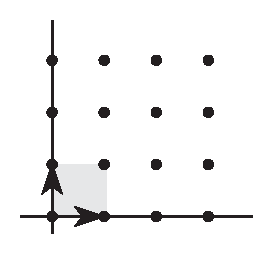
\includegraphics{lbasisa} 
   &
  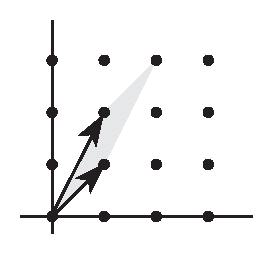
\includegraphics{lbasisb} \\
  (a) & (b)
 \end{tabular}
\end{center}
\caption{Two different bases for ${\protect\Z} \times {\protect\Z}$
     \label{Lattice:Basis:Fig}}
\end{figure}

A new geometric method of proving these results was given by {\Minkowski}
by his development of the \key{geometry of numbers}.  In this chapter
we follow {\Minkowski}'s lead and use these geometric techniques.  A
significant advantage of the geometric approach is the recent
development of (relatively) efficient algorithms for solving
multidimensional approximation problems like those mentioned above.
In addition to solving problems in diophantine approximation, these
algorithms can also be used to find relations between numbers and to
factor polynomials. 

\section{Lattice Fundamentals}
\label{Lattice:Fund:Sec}

The elements of $\mathbb{R}^{n}$ are $n$-tuples that for an additive group by 
component-wise addition. Multiplication by an element $a \in \mathbb{R}$ 
maps $\vec v = \langle v_1, v_2, \ldots, v_n \rangle \in \R^n$ to 
$a \vec v = \langle av_1, av_2, \ldots, a v_n \rangle$.

A \keyi{lattice} is a discrete subset of $\mathbb{R}^{n}$ that 
can be generated by $n$ linearly independent vectors: 
\begin{equation*}
{\cal L} = \{\, \lambda_{1} \vec b_{1} + \cdots + \lambda_{n} \vec b_{n} \mid
\lambda_{i} \in \Z \,\}.
\end{equation*}
We call $\{\vec b_{1}, \ldots, \vec b_{n}\}$ a {\em
basis}\index{lattice!  basis of} of the lattice ${\cal L}$.  As illustrated
in \figref{Lattice:Basis:Fig}, a lattice can have more than one basis.
In this case, the lattice is ${\cal L} = \Z \times \Z$.  In
\figref{Lattice:Basis:Fig}(a) we have shown the natural basis $\vec b_{1} =
(1, 0)$ and $\vec b_{2} = (0, 1)$, while \figref{Lattice:Basis:Fig}(b)
shows the alternative basis $\vec b_{1}' = (1, 2)$ and $\vec b_{2}' = (1, 1)$.
 
Each of these two figures includes a shaded parallelepiped defined by
the two basis vectors.  Each shaded region is called the
\keyi{fundamental domain} of the corresponding basis.  Repeated copies
of the fundamental domain \key{tessellate} $\mathbb{R}^{n}$.  As we shall see,
the volume of fundamental domain of a lattice is independent of the
basis used to define it.

The geometric properties of a lattice are induced by the definition
used for distance.  For all applications with which we are concerned,
the distance between two points is invariant under rigid translations
of the two points.  Thus the distance between the two points $\vec{x}$
and $\vec{y}$ is the length of the vector between them---that is, the
length of $\vec{x}-\vec{y}$.  When given suitable properties, a function
that maps vectors in $\Re^n$ into their length is called a \textbf{norm}.
We will only consider distance measures that are derived from norms.

\begin{definition}
A {\bf norm}\index{norm! of a lattice} on $\mathbb{R}^{n}$ is a map 
$d: \mathbb{R}^{n} \rightarrow \mathbb{R}$ such that 
\begin{enumerate}
\item $d(x) \ge 0$ for all $x \in \mathbb{R}^{n}$,
\item $d(x) = 0$ if and only if $x = 0$,
\item $d(\alpha x) = |\alpha| d(x)$, for $\alpha \in \mathbb{R}$,
\item $d(x+y) \le d(x) + d(y)$.
\end{enumerate}
\end{definition}

Each of these conditions has a natural geometric interpretation.  The
first two conditions say that the length of every vector other than
$(0, \ldots, 0)$ is positive.  The third says that if we scale the
entire space by a factor of $\alpha$ then the length of the vector
increases by a factor of $|\alpha|$.  The fourth condition is the
triangle inequality.

A frequently used collection of norms are the {\em
$p$-norms},\index{p-norm of a lattice@$p$-norm of a lattice} which are
denoted by $\|\;\|_{p}$.  If $x = (x_{1}, \ldots, x_{n})$ is a point
in $\mathbb{R}^{n}$, then $\|x\|_{p}$ is defined to be
\[
\|x\|_{p} = \sqrt[p]{|x_{1}|^{p} + |x_{2}|^{p} + \cdots + |x_{n}|^{p}}.
\]
Useful special cases of the $p$ norm are the $1$-norm of $x$,
$\|x\|_{1}$; the \keyi{Euclidean norm}, $\|x\| = \|x\|_{2}$; and the
maximum norm $\|x\|_{\infty}$.  The $1$-norm of $x$ is defined by
\[
\|x\|_{1} = |x_{1}| + |x_{2}| + \cdots + |x_{n}|,
\]
which is the ``Manhattan'' length of $x$.\index{Manhattan length} The
Euclidean distance function\index{Euclidean distance} is just the $2$-norm:
\[
\|x\|_{2} = \sqrt{|x_{1}|^{2} + |x_{2}|^{2} + \cdots + |x_{n}|^{2}}.
\]
The \keyi{maximum norm} is the limit of $\|x\|_{p}$ as $p$ goes to
infinity:
\[
\|x\|_{\infty} = \max (|x_{1}|, \ldots, |x_{n}|).
\]
All of the $p$-norms generate the same topology on $\mathbb{R}^{n}$.
\addsymbol{$\|\vec{v}\|_p$}{$p$ norm of a vector}
\addsymbol{$\|\vec{v}\|$}{$2$ norm of a vector, Euclidean distance}
\addsymbol{$|\vec{v}|$}{$\infty$ norm of a vector, sum of absolute
values of its components}

The fact that the $p$-norms are norms follows from the \keyi{Minkowski
inequality} \cite[pages 115--117]{Minkowski2018-iz}:

\begin{proposition}[{\Minkowski}]
If $x_1, \ldots, x_n$ and $y_1, \ldots, y_n$ are non-nega\-tive real
numbers, then for all $p \ge 1$
\[
\left(|x_1 + y_1|^p + \cdots + |x_n + y_n|^p\right)^{1/p} \le 
\left(x_1^p + \cdots + x_n^p\right)^{1/p} + 
\left(y_1^p + \cdots + y_n^p\right)^{1/p}.
\]
\end{proposition}

\noindent
A proof of this proposition can be found in \cite{Hardy1952-ad}.\Marginpar{Include the proof here.}

Determining whether a set of points is a lattice can be quite
difficult, if the set is not specified in terms of set of basis
vectors.  In this situation the following proposition is quite useful.
For a proof see {\Cassels} \cite[page 78]{Cassels2012-kd}.

\begin{proposition} \label{Lattice:Condition:Prop}
A necessary and sufficient condition that a set of points ${\cal L} \subset
\mathbb{R}^n$ be a lattice is that the set satisfy:
\begin{itemize}
\item ${\cal L}$ is closed under component-wise addition,
\item ${\cal L}$ contains $n$ linearly independent points,
\item There exists a constant $\eta> 0$ such that if $(x_1, \ldots,
x_n) \in {\cal L}$ and
\[
\sqrt{x_1^2 + \cdots + x_n^2} < \eta,
\]
then $x_1 = x_2 = \cdots = x_n = 0$.
\end{itemize}
\end{proposition}

The first two conditions ensure that there is a basis for the points
of ${\cal L}$.  The third condition states that there is a neighborhood of
the origin that contains only one point.  This ensures that all the
points of ${\cal L}$ are separated and thus the basis is a $\Z$ lattice.

\paragraph{Fundamental Domains}

\begin{figure}
\begin {center}
 \begin {tabular}{cc}
   \begin{picture}(150, 62)
     \put(0,0){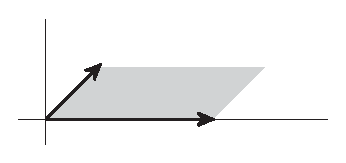
\includegraphics{FundDoma}}
     \put(85,0){$\vec{a}$}
     \put(30,42){$\vec{b}$}
   \end{picture}
  & 
   \begin{picture}(150, 62)
     \put(0,0){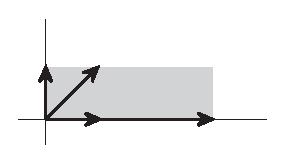
\includegraphics{FundDomb}}
     \put(100,0){$\vec{a}$}
     \put(40,42){$\vec{b}$}
     \put(40,0){$\vec{b}_{\parallel}$}
     \put(3,42){$\vec{b}_{\perp}$}
   \end{picture} \\
   (a) & (b) 
 \end{tabular}
\end{center}
\caption{Computing the Area of a
Parallelogram\label{Lat:Parallel:Fig}}
\end{figure}

The volume of the fundamental domain is an important property of a
lattice.  As we shall show, it does not depend on the basis, but is an
invariant of the lattice.  If the basis vectors are orthogonal then
the volume of fundamental domain is just the product of the lengths of
the vectors.  Recall that two vectors $\vec{a}$ and $\vec{b}$ are
orthogonal if and only if their {\em dot product}\index{dot product!of two
vectors} vanishes
\[
\vec{a} \cdot \vec{b} = a_1 b_1 + \cdots + a_n b_n = 0.
\]
To compute the volume of a general parallelepiped we modify
the basis vectors in such a way that the volume is left unchanged, but
the new vectors are orthogonal.  This is illustrated in
\figref{Lat:Parallel:Fig}. 
\addsymbol{$\vec{a}\cdot\vec{b}$}{Dot product of $\vec{a}$ and
$\vec{b}$, $a_1 b_1 + \cdots + a_n b_n$}

The area of the parallelogram bounded by the vectors $\vec{a}$ and
$\vec{b}$ is the same as that of the rectangle in
\figref{Lat:Parallel:Fig}(b).  In \figref{Lat:Parallel:Fig}(b), we
have decomposed $\vec{b}$ into the sum of two orthogonal vectors
$\vec{b}_{\perp}$ and $\vec{b}_{\parallel}$.  $\vec{b}_{\parallel}$ is
the portion of $\vec{b}$ that is parallel to $\vec{a}$ and does not
contribute to the area of the parallelogram.  Thus, the area delimited
by $\vec{b}_{\perp}$ and $\vec{a}$ is the same as that
delimited by $\vec{a}$ and $\vec{b}$.  The magnitude of
$\vec{b}_{\parallel}$ is $\vec{b} \cdot \vec{a}$, so 
\[
\vec{b}_{\perp} = \vec{b} - \frac{\vec{b} \cdot \vec{a}}{\|\vec{a}\|} \,
\frac{\vec{a}}{\|\vec{a}\|} = 
\vec{b} - \frac{\vec{b} \cdot \vec{a}}{\vec{a} \cdot \vec{a}}\,
\vec{a}\;,
\]
where the second factor is the unit vector parallel to $\vec{a}$.
So, if we denote by $\vec{b}^{\ast} = \vec{b}_{\perp}$ and
$\vec{a}^{\ast} = \vec{a}$ the orthogonalization of $\vec{a}$ and
$\vec{b}$ we have
\[
\left(\begin{array}{c} \vec{a} \\ \vec{b} \end{array}\right)
= 
\left(\begin{array}{cc} 1 & 0 \\ 
\frac{\vec{b} \cdot \vec{a}}{\vec{a} \cdot \vec{a}} & 1 \end{array}\right)
\cdot
\left(\begin{array}{c} \vec{a}^{\ast} \\ \vec{b}^\ast \end{array}
\right)
\]
More generally, we can orthogonalize the vectors $\vec{a}_1, \ldots,
\vec{a}_n$ as follows
\[
\begin{array}{l} \vec{a}_1 = \vec{a}^{\ast}_1 \\ \vec{a}_2 \\ \vec{a}_3 \\ \vdots \\ \vec{a}_n \end{array}
\Rightarrow
\begin{array}{l} \vec{a}^{\ast}_1 \\ 
   \vec{a}_2 -\mu_{21} \vec{a}^{\ast}_1 = \vec{a}^{\ast}_2 \\
   \vec{a}_3 - \mu_{31} \vec{a}^{\ast}_1\\ \vdots \\ \vec{a}_n -\mu_{n1} \vec{a}^{\ast}_1
\end{array}
\Rightarrow
\begin{array}{l} \vec{a}^{\ast}_1 \\ 
   \vec{a}^{\ast}_2 \\ 
   (\vec{a}_3 - \mu_{31} \vec{a}^{\ast}_1) - \mu_{32}\vec{a}^{\ast}_2 = \vec{a}^{\ast}_3 \\ 
   \vdots \\ (\vec{a}_n -\mu_{n1} \vec{a}^{\ast}_1)  - \mu_{n2}\vec{a}^{\ast}_2 
\end{array}
\Rightarrow
\cdots
\]
where the $\vec{a}^{\ast}_i$ are elements of the final orthogonal
basis.  The number $\mu_{ij}$ is the magnitude of the component of
$\vec{a}_i$ parallel to $\vec{a}^{\ast}_j$.

The computation of the orthogonal basis is initiated by setting
$\vec{a}^{\ast}_1 = \vec{a}_1$.  At the $i$-th step, each of the
remaining vectors (numbered $i+1$ through $n$) is modified so as to be
orthogonal to $\vec{a}^{\ast}_i$.  This process is called the
(modified) {\em Gram-Schmidt orthogonalization
process}.\index{Gram-Schmidt algorithm} The following code makes this
procedure precise.

\begindsacode
GramSchmidt ($\vec{a}_1, \ldots, \vec{a}_n$) := $\{$\\
\>loo\=p for $i = 1, \ldots, n$  do \{ \\
\>\> $\vec{a}^{\ast}_i \leftarrow \vec{a}_i$; \\
\>\> \} \\
\>loop for $i = 1, \ldots, n$  do \{ \\
\>\> loo\=p for $j = i+1, \ldots, n$ do \{\\
\>\> \> $\vec{a}^{\ast}_j \leftarrow \vec{a}^{\ast}_j 
     - (\vec{a}^{\ast}_j \cdot \vec{a}^{\ast}_i)/(\vec{a}^{\ast}_i \cdot \vec{a}^{\ast}_i) \vec{a}^{\ast}_i$; \\
\>\>\> \} \\
\>\> \} \\
\>return ($\vec{a}^{\ast}_1, \ldots, \vec{a}^{\ast}_n$); \\
\>$\}$
\enddsacode

If the vectors $\vec{a}_1, \ldots, \vec{a}_n$ are arranged to form a
matrix $A$, we see that the Gram-Schmidt process factors $A$ into two
matrices as follows:
\begin{equation} \label{Gram:Schmidt:Eq}
\begin{aligned}
\left(
 \begin{array}{c}
   \vec{a}_1 \\ \vec{a}_2 \\ \vec{a}_3 \\ \vdots \\ \vec{a}_n
 \end{array}
\right)
 & = 
\left(
 \begin{array}{cccccc}
   1 & 0 & 0 & \cdots & 0 & 0 \\ 
   \mu_{21} & 1 & 0 & \cdots & 0 & 0 \\ 
   \mu_{31} & \mu_{32} & 1 & \cdots & 0 & 0 \\
   \vdots & & \vdots & & & \vdots \\ 
   \mu_{n1} & \mu_{n2} & \mu_{n3} & \cdots & \mu_{n,n-1} & 1
 \end{array}
\right)
\cdot 
\left(
 \begin{array}{c}
   \vec{a}^{\ast}_1 \\ \vec{a}^{\ast}_2 \\ \vec{a}^{\ast}_3 \\ 
   \vdots \\ \vec{a}^{\ast}_n
 \end{array}
\right) \\
 & = Q \cdot A^{\ast}
\end{aligned}
\end{equation}
The determinant of $A^{\ast}$ is the product of the lengths of the
(orthogonal) basis vectors $\vec{a}^{\ast}_i$ as we show in
\propref{Hadamard:Ineq:Prop}.
Taking the determinant of the previous equation, we have
\[
\begin{aligned}
  \det A & = (\det Q) (\det A^{\ast}) \\
    & = \|\vec{a}^{\ast}_1\| \cdots \|\vec{a}^{\ast}_n\| = \det {\cal L},
\end{aligned}
\]
since the determinant of $Q$ is $1$.
Thus the volume of the fundamental domain of a lattice is identical to
the determinant of the lattice.  This is stated formally in
\propref{Parallelepiped:Vol:Prop}.  

\begin{proposition}\label{Parallelepiped:Vol:Prop}
The volume of the parallelepiped $\Delta$ bounded by the vectors
$\{\vec{a}_{1}, \ldots, \vec{a}_{n}\}$ is
\[
\vol(\Delta) = \left|
\begin{array}{ccc}
a_{11} & \cdots & a_{1n} \\
\vdots &   & \vdots \\
a_{n1} & \cdots & a_{nn}
\end{array}
\right|,
\]
where $\vec{a}_{i} = (a_{i1}, a_{i2}, \ldots, a_{in})$.
\end{proposition}

\smallskip
The above discussion used a special case of the following proposition due to
{\Hadamard} \cite{Hadamard1893-xq}. 

\begin{proposition}[Hadamard] \label{Hadamard:Ineq:Prop}
Let $\vec a_{i} = (a_{i1}, \ldots, a_{in})$ be $n$ vectors whose
components lie in $\C$, then
\[
A = \det\left( \begin{array}{c} \vec{a}_1 \\ \cdots \\ \vec{a}_n \end{array}\right)
 = \left|
 \begin{array}{cccc}
a_{11} & \cdots & a_{1n} \\
\vdots &  & \vdots \\
a_{n1} & \cdots & a_{nn} 
\end{array}
\right| \le
\prod_{1 \le i \le n} \|\vec a_{i} \|.
\]
Equality is achieved if and only if the rows of the determinant are
orthogonal. 
\end{proposition}

Intuitively, this theorem can be justified as follows.  By
\propref{Parallelepiped:Vol:Prop} the determinant is the volume of the
parallelepiped with edges $\vec{a}_i$.  This volume is maximized when
the edge vectors are orthogonal (all the corners of the
parallelepiped are right angles).  \Eg, a rectangle has the largest
area of all parallelograms with specified edge lengths.  In the
orthogonal case the volume of the parallelepiped is the product on
the right.  

This argument is circular since we used Hadamard's proposition to show
that the volume of a parallelepiped was the determinant of the
appropriate matrix.  The following proof does not have this problem. 

\begin{proof} 
We proceed by contradiction.
Without loss of generality, we can assume each vector $\vec{a}_i$  has
length $1$.  Assume the $\vec{a}_i$ are chosen so as to 
maximize $A$.  Since the identity matrix satisfies all the conditions
of the proposition and has determinant $1$, so
$A > 1$.  Now assume that the first two rows of $A$ are not
orthogonal.  We shall show that $A$ cannot then be maximal.
\addsymbol{$\overline{\protect\vphantom{b}a}$}{Complex conjugate of $a$}

We have
\[
C = \sum_{1 \le j \le n}\overline{\vphantom{b}a_{1j}} a_{2j},
\]
where the overbar in $\overline{\vphantom{b}a_{1j}}$ indicates the
\keyi{complex conjugate}. 
Construct a new matrix whose second row is orthogonal to the first,
but which is otherwise unchanged, \ie, $a'_{2j} = \lambda a_{1j} + \mu
a_{2j}$ such that
\[
\sum_{1 \le j \le n} a'_{2j} \overline{\vphantom{b}a_{1j}} = 0
\qquad\mbox{and}\qquad
\sum_{1 \le j \le n} |a'_{2j}|^2 = 1.
\]
Denote the determinant of this new matrix by $A' = \mu A$.

Replacing $a'_{2j}$ by $\lambda a_{1j} + \mu a_{2j}$ in the first
summation gives $\lambda + \mu C = 0$.  Proceeding similarly with the
second summation:
\[
\begin{aligned}
\sum_{1 \le j \le n} |a'_{2j}|^2  & = 
\sum_{1 \le j \le n} (\lambda a_{1j} + \mu a_{2j}) 
  (\overline{\lambda} \overline{\vphantom{b}a_{1j}} + \overline{\vphantom{b}\mu}
\overline{\vphantom{b}a_{2j}})  \\
  & = |\lambda|^2 + \mu \overline{\lambda} C 
        + \lambda \overline{\vphantom{b}\mu}\overline{C} + |\mu|^2 = 1.
\end{aligned}
\]
Using $\lambda + \mu C = 0$ to eliminate $\lambda$ we have 
$|\mu|^2 ( 1 - |C|^2) = 1$, or $|\mu|^2 > 1$, which contradicts the
claim that $A$ was maximal.  Thus the matrix achieves its maximal
value when the rows are orthogonal.

Since we now know that the rows are orthogonal we can compute the
determinant quite easily.  The product of the matrix with the complex
conjugate of its transpose is
\[
\left(
 \begin{array}{cccc}
a_{11} & \cdots & a_{1n} \\
\vdots &  & \vdots \\
a_{n1} & \cdots & a_{nn} 
\end{array}
\right)
\cdot
\left(
 \begin{array}{cccc}
\overline{\vphantom{b}a_{11}} & \cdots & \overline{\vphantom{b}a_{n1}} \\
\vdots &  & \vdots \\
\overline{\vphantom{b}a_{1n}} & \cdots & \overline{\vphantom{b}a_{nn}} 
\end{array}
\right) =
\left(\sum_{1 \le k \le n} a_{ik} \overline{\vphantom{b}a_{jk}}\right)_{i,j}
= {\bf 1}.
\]
So $A = 1$, as desired.
\end{proof}


\begin{proposition}
The volume of the fundamental domain of a lattice is independent of
the basis used to compute it.
\end{proposition}

\begin{proof}
Let ${\cal L}$ be the lattice generated by the vectors $\{\vec{b}_i\}$ and
let $\{\vec{b}'_i\}$ be a different basis for ${\cal L}$.  Since each of
the vectors $\vec{b}'_i$ is an element of ${\cal L}$, each $\vec{b}'_i$ can
be represented as a linear combination of the $\vec{b}_i$:
\[
\vec b_{i}' = a_{i1} \vec b_{1} + a_{i2} \vec b_{2} + \cdots + a_{in} \vec b_{n},
\qquad 1 \le i \le n,
\]
where the $a_{ij}$ are elements of $\Z$.  Similarly, there exist
$a'_{ij}$ such that
\[
\vec b_{j} = a_{j1}' \vec b_{1}' + a_{j2}' \vec b_{2}' + \cdots + a_{jn}'
\vec b_{n}',
\qquad 1 \le j \le n.
\]
Define the transformation matrices $A =
(a_{ij})$ and $A' = (a_{ij}')$.
Composing these two transformations leaves a basis unchanged, so $AA'
= A' A = I$.  Thus the volume of the fundamental region of a lattice is 
independent of the basis chosen.  
It is denoted by $\det({\cal L})$.
\end{proof}

\paragraph{Sub-Lattices}

A subset of a lattice that is also a lattice is called a
\keyi{sub-lattice}.  Let $\vec{a}_1, \ldots, \vec{a}_n$ be linearly
independent elements of the lattice ${\cal L}$.  They are the basis of
a second lattice ${\cal M}$, which is a sub-lattice of ${\cal L}$.
Since the $\vec{a}_i$ are elements of ${\cal L}$ they can be written
as
\begin{equation} \label{SubLatt:a:Eq}
\vec{a}_i = \sum_j v_{ij} \vec{b}_j.
\end{equation}

Taking the determinant of these equations gives
\[
\det {\cal M} = \det (v_{ij}) \cdot \det {\cal L}.
\]
The {\em index}\index{index!of a sub-lattice} of ${\cal L}$ is defined
to be 
\begin{equation} \label{Latt:Index:Eq}
I = \det (v_{ij}) = \frac{\det {\cal M}}{\det {\cal L}}.
\end{equation}
The index of a sub-lattice is independent of the choice of bases.
The linear equations \eqnref{SubLatt:a:Eq} can be solved for the
$\vec{b}_j$ as linear combinations of the $\vec{a}_i$.  The
denominators of these coefficients is $\det(v_{ij}) = i$.  So we have
\[
I \vec{b}_j = \sum_i w_{ij} \vec{a}_{i},
\]
where the $w_{ij}$ are rational integers.  Thus, $I {\cal L} \subseteq
{\cal M} \subseteq {\cal L}$.

The following proposition shows that a basis can be found for the
sub-lattice ${\cal M}$ with a very specific structure.

\begin{proposition} \label{SubLattice:Basis:Prop}
Let ${\cal M}$ be a sub-lattice of ${\cal L} = (\vec{b}_1, \ldots,
\vec{b}_n)$.  Then a basis, $\vec{a}_1, \ldots, \vec{a}_n$ for ${\cal
M}$ can be found such that 
\begin{equation} \label{SubLatt:Basis:Eq}
\begin{aligned}
\vec{a}_1 & = v_{11} \vec{b}_1, \\
\vec{a}_2 & = v_{21} \vec{b}_1 + v_{22} \vec{b}_2, \\
  & \vdots \\
\vec{a}_n & = v_{n1} \vec{b}_1 + \cdots + v_{n2} \vec{b}_n,
\end{aligned}
\end{equation}
where the $v_{ij}$ are integers and $v_{ii}$ are positive.
Conversely, for every basis $\vec{a}_1, \ldots, \vec{a}_n$ of ${\cal
M}$ there exists a basis $\vec{b}_1, \ldots, \vec{b}_n$ such that
\eqnref{SubLatt:Basis:Eq} holds with integer $v_{ij}$.
\end{proposition}

\begin{proof}
We start with the forward direction, with a basis $\vec{b}_1, \ldots,
\vec{b}_n$ of ${\cal L}$.  Since ${\cal M}$ is a sub-lattice of ${\cal
L}$, every element of ${\cal M}$ can be uniquely written as
\[
c_{i1} \vec{b}_1 + c_{i2} \vec{b}_2 + \cdots c_{in} \vec{b}_n,
\]
where the $c_{ij}$ are integers.  Of all these elements we choose an
element with smallest positive $c_n$.  Denote this element by 
\[
\vec{a}_n = c_{1n} \vec{b}_1 + \cdots c_{nn} \vec{b}_n.
\]

We claim that $c_{nn}$ divides the
coefficient of $\vec{b}_n$ of every element of ${\cal M}$.  If this
were not the case there would be a
\[
\vec{a}^{\ast} = c_1^{\ast} \vec{b}_1 + \cdots c_n^{\ast} \vec{b}_n
\]
such that the greatest common divisor of $c_n^{\ast}$ and $c_{nn}$,
$d$ lies between $0$ and $c_{nn}$.  But then there would be $A$ and
$B$ such that $A c^{\ast}_n + B c_{nn} = d$.  Thus,
\[
A \vec{a}_n + B \vec{a}^{\ast} = c^{\ast\ast}_1 \vec{b}_1 + \cdots + d
\vec{b}_n,
\]
whose coefficient of $\vec{b}_n$ is not divisible by $c_{nn}$.  

Continuing this process for the coefficient of $\vec{b}_{n-1}$ we have
\[
\begin{aligned}
\vec{a}_1 & = c_{11} \vec{b}_1,  \\
\vec{a}_2 & = c_{21} \vec{b}_1 + c_{22} \vec{b}_2,  \\
   & \vdots \\
\vec{a}_n & = c_{n1} \vec{b}_1 + \cdots + c_{nn} \vec{b}_n,  
\end{aligned}
\]
and the $c_{ii}$ are as small as possible.  These vectors are 
linearly independent and every element of ${\cal M}$ is a linear
combination of the $\vec{a}_i$ by the reasoning above. 

In the converse direction, since $I {\cal L}$ is contained in ${\cal
M}$, we have
\[
\begin{aligned}
I \vec{b}_1 & = v_{11} \vec{a}_1,  \\
I \vec{b}_2 & = v_{21} \vec{a}_1 + v_{22} \vec{a}_2,  \\
   & \vdots \\
I \vec{b}_n & = v_{n1} \vec{a}_1 + \cdots + v_{nn} \vec{a}_n,  
\end{aligned}
\]
where the $v_{ij}$ are integers.  The system can be solved to produce
\[
\begin{aligned}
\vec{a}_1 & = w_{11} \vec{b}_1,  \\
\vec{a}_2 & = w_{21} \vec{b}_1 + w_{22} \vec{b}_2,  \\
   & \vdots \\
\vec{a}_n & = w_{n1} \vec{b}_1 + \cdots + w_{nn} \vec{b}_n,  
\end{aligned}
\]
where the the $w_{ij}$ may be rational numbers.  Since the $\vec{b}_i$
are a basis of ${\cal L}$ and the $\vec{a}_i$ are elements of ${\cal
L}$ the the $w_{ij}$ are actually integers.
\end{proof}

Since both a sub-lattice and a lattice are additive groups, we can
form the quotient of ${\cal L}/{\cal M}$.  The sub-lattice has a
larger fundamental domain than that of ${\cal L}$.  We can think of
the fundamental domain of ${\cal L}$ tiling the fundamental domain of
${\cal M}$.    This suggests that the number of elements of ${\cal
L}/{\cal M}$ is equal to the index of ${\cal M}$ in ${\cal L}$.  This
is the case as is shown in the proof of the following proposition.

\begin{proposition} \label{SubLattice:Index:Prop}
Let ${\cal M}$ be a sub-lattice of ${\cal L}$.  Then the number of
elements of ${\cal L}/{\cal M}$ is equal to the index of ${\cal M}$ in
${\cal L}$, $\det {\cal M}/\det {\cal L}$.
\end{proposition}

\begin{proof}
By \propref{SubLattice:Basis:Prop}, ${\cal M}$ has a basis that can be
represented in terms of the basis vectors of ${\cal L}$ as in
\eqnref{SubLatt:Basis:Eq}.  By reduction with respect to this basis,
an element of ${\cal L}/{\cal M}$ is of the form
\[
u_1 \vec{b}_1 + u_2 \vec{b}_2 + \cdots + u_n \vec{b}_n,
\]
where $0 \le u_i < v_{ii}$.  Therefore, there are 
\[
v_{11} v_{22} \cdots v_{nn}
\]
elements in ${\cal L}/{\cal M}$.  But this is the index of ${\cal M}$
in ${\cal L}$.
\end{proof}

\section{Minkowski Convex Body Theorem}
\index{Minkowski convex body theorem|(}

Intuitively, a convex body in $\mathbb{R}^{n}$ is region of $\mathbb{R}^{n}$ that has
no holes or surface depressions.  Let $C$ be an $n$-dimensional
bounded subset of $\mathbb{R}^n$.  We call such a set a {\em body}.  $C$ is
said to be {\em convex}\index{convex body} if, for every pair of
points $x$, $y$ in $C$ and real number $\mu \in [0, 1]$, $\mu x + (1 -
\mu) y$ is also in $C$.  A convex body $C$ is {\em
symmetric}\index{convex body!symmetric} if, for every $x \in C$, $-x$
is also in $C$.  Thus a symmetric \key{convex body} includes the origin.

\begin{proposition}[{\Minkowski}]
Let $C$ be a symmetric convex body in $\mathbb{R}^{n}$, ${\cal L}$ a lattice in
$\mathbb{R}^{n}$.  If either
\[
\vol C > 2^n \det {\cal L}
\]
or 
\[
\vol C = 2^n \det {\cal L}, \quad \mbox{and $C$ is compact}
\]
then $C$ contains a non-zero element of ${\cal L}$.
\label{Minkowski:Convex:Prop}
\end{proposition}

\begin{proof}
Let $\Delta$ be a fundamental domain of ${\cal L}$ with respect to some basis,
$\vol \Delta = \det {\cal L}$.  Let $C' = \frac{1}{2}C$, \ie\ each point has
all of its coordinates multiplied by $\frac{1}{2}$, so 
\[
\vol C' = \frac{1}{2^{n}} \vol C.
\]
Initially, assume $\vol C' > \vol \Delta$.  $C'$ only intersects a
finite number of fundamental domains of ${\cal L}$ (since $C'$ is finite and
thus its closure is compact).  Denote these regions by
$\ell_{1}+\Delta, \ldots, \ell_{r}+\Delta$.  The volume of $C'$ is 
\begin{equation}
\vol(C') = \vol(C' \cap (\ell_{1}+\Delta)) + \cdots +
\vol(C' \cap (\ell_{r}+\Delta)).
\label{Mink:Vol:Eq}
\end{equation}
The volume of $C' \cap (\ell + \Delta)$ is the same as $(C' - \ell) \cap
\Delta$.  Instead of shifting $\Delta$ to intersect $C'$, we shift $C'$
to intersect $\Delta$:
\[
\vol C' = \vol((C' - \ell_{1}) \cap \Delta) + \cdots +
\vol((C' - \ell_{r}) \cap \Delta)
> \vol(\Delta).
\]
There are at least two sets $C' - \ell_{i}$ and $C' -\ell_{i}$ that are
not disjoint.  So there are $x', y' \in C'$ such that $x' - \ell_{i} = y' -
\ell_{j}$.  Consider the lattice point 
\[
\ell_{j} - \ell_{i} = y' - x' = \frac{1}{2}y - \frac{1}{2}x.
\]
Since $x$ and $y$ are in $C$, by convexity and symmetry of $C$, the
lattice point $\ell_{j} - \ell_{i}$ is in $C$.

Now assume that $C$ is compact and  $\vol C' = \vol \Delta$.  In this case we enlarge $C$
slightly so that the previous case applies.  If $m$ is some positive number
then
\[
\vol\left(\left(1+\frac{1}{m}\right)C\right) = \left[1+\frac{1}{m}\right]^{n} \vol(C)
> 2^{n} \vol(\Delta).
\]
By the previous discussion $(1+\frac{1}{m})C \cap {\cal L} \not= \{0\}$, \ie\
it contains a non-zero element.  As $m$ goes to infinity
\[
\left(1+\frac{1}{m}\right)C \supseteq \left(1+\frac{1}{m+1}\right)C 
\supseteq \left(1+\frac{1}{m+2}\right)C \supseteq \cdots.
\]
Each of $(1+\frac{1}{m})C \cap {\cal L} -\{0\}$ is non-empty.  Eventually they
must all be the same since the lattice ${\cal L}$ is discrete.  Since $C$ is compact
\[
\bigcap_{m>0} \left(1+ \frac{1}{m}\right) C = C,
\]
$C \cap {\cal L} - \{0\}$ must also be non-empty.
\end{proof}

\paragraph{Dirichlet's Theorems}

{\Minkowski}'s theorem yields easy proofs of Propositions
\ref{Dirichlet:Multiple:Prop} and \ref{Dirichlet:Mutual:Prop}.  
To prove \propref{Dirichlet:Multiple:Prop} for arbitrary $n$, we use
the lattice generated by:
\[
\left(\begin {array}{c} 
  \vec{b}_0 \\ \vec{b}_1 \\ \vec{b}_2 \\ \vdots \\ \vec{b}_n 
\end{array}\right)
=
\left(\begin {array}{ccccc}
  \epsilon^n & \alpha_1/\epsilon & \alpha_2/\epsilon & 
    \ldots & \alpha_n/\epsilon \\
  0 & 1/\epsilon & 0 & \ldots & 0 \\
  0 & 0 & 1/\epsilon & \ldots & 0 \\
  \vdots  & & \vdots & &\vdots \\
  0 & 0 & 0 & \ldots & 1/\epsilon
\end{array}
\right).
\]
The volume of the fundamental domain of this lattice is clearly 1.
The $n+1$ dimensional cube, $|x_i| \le 1$, is a convex body with
volume $2^{n+1}$ satisfying the convex body theorem.

For the point $q \vec{b}_0 - p_1 \vec{b}_1 - \cdots - p_n \vec{b}_n$
to lie in the cube the following inequalities must hold.
\[
\begin{aligned}
|q\epsilon^n| &\le 1, \qquad \Longrightarrow\qquad 
    \frac{1}{|q|^{1/n}} \ge \epsilon, \\
|p_i - q \alpha_i| &\le \epsilon.
\end{aligned}
\]
Combining these two inequalities gives 
\propref{Dirichlet:Multiple:Prop}.

To prove \propref{Dirichlet:Mutual:Prop} we use the lattice
\begin{equation} \label{Dirichlet:Lattice:Eq}
\left(
\begin{array}{c}
  \vec{b}_0 \\ \vec{b}_1 \\ \vec{b}_2 \\ \vdots \\ \vec{b}_n
\end{array}\right) =
\left(\begin{array}{cccccc}
1/\epsilon &  0 & 0 & \ldots & 0 \\
\alpha_1/\epsilon & \epsilon^{1/n} & 0 & \ldots & 0 \\
\alpha_2/\epsilon & 0 & \epsilon^{1/n} & \ldots & 0  \\
\vdots  & & \vdots & & \vdots \\
\alpha_n/\epsilon & 0 & 0 & \ldots & \epsilon^{1/n}
\end{array}\right).
\end{equation}
Again by the convex body theorem, there exist integers $p_0, p_1,
\ldots, p_n$ such that $p_0 \vec{b}_0 + p_1 \vec{b}_1 + \cdots + p_n
\vec{b}_n$ lies within the cube $|x_i| \le 1$.  Examining the
components of this vector we see that
\[
\left| p_0 + p_1 \alpha_1 + \cdots p_n \alpha_n\right| \le \epsilon,
\]
and 
\[
\left|p_i\right| \le \epsilon^{-1/n}, \quad \mbox{for $1 \le i \le n$}
\]
as desired.
\index{Minkowski convex body theorem|)}

\section{Reduced Bases}
\label{Lovasz:Basis:Sec}

The previous sections of this chapter have illustrated how many
problems can be phrased in terms of finding short vectors in a
lattice.  In this section, we look at the algorithmic problem of
finding short vectors.  If the basis vectors of a lattice are
orthogonal, then the shortest vector in the lattice will be one
of the basis vectors.  Not all lattices have orthogonal bases, but
this provides one approach to the short vector problem.  We seek a
sequence of unimodular transformations\index{unimodular matrix} that
yields a new set of basis vectors that are as close to orthogonal as
possible.  Then the smallest vector of this ``nearly orthogonal''
basis will be short. 

Let $\vec{b}_1, \ldots, \vec{b}_n$ be the basis for a lattice ${\cal L}$, and
let 
\[
\vec{v} = \lambda_1 \vec{b}_1 + \cdots + \lambda_n \vec{b}_n,
\]
be a short vector in ${\cal L}$.  By Cramer's rule and
\propref{Hadamard:Ineq:Prop}, we can bound $\lambda_i$ by 
\[
\begin{aligned}
  |\lambda_i| & = \left|\frac{\det(\vec{b}_1, \ldots, \vec{b}_{i-1},
\vec{v}, \vec{b}_{i+1}, \ldots, \vec{b}_n)}{\det(\vec{b}_1, \ldots,
\vec{b}_n)} \right|, \\
  & \le \frac{\|\vec{b}_1\| \cdots \|\vec{b}_{i-1}\|\, \|\vec{v}\|\,
\|\vec{b}_{i+1}\| \cdots \|\vec{b}_n\|}{\left|\det(\vec{b}_1, \ldots,
\vec{b}_n)\right| }.
\end{aligned}
\]
Assuming $\vec{v}$ is no larger than the smallest basis vector, we
have
\[
|\lambda_i | \le  \frac{\|\vec{b}_1\|
\cdots\|\vec{b}_n\|}{\left|\det(\vec{b}_1, \ldots, \vec{b}_n)\right|} = \delta,
\]
where we call $\delta$ the \keyi{orthogonality defect} of the basis
$\vec{b}_1, \ldots, \vec{b}_n$.

So the short vectors of a lattice are those of the form
\[
\lambda_1 \vec{b}_1 + \cdots + \lambda_n \vec{b}_n , \quad |\lambda_i|
\le \delta.
\]
When $\vec{b}_1, \ldots, \vec{b}_n$ are orthogonal, $\delta = 1$ and
there are only $3^n$ candidates.  However, by the triangle inequality,
the shortest vector must be one of the basis vectors.  We state this
formally as,

\begin{proposition} \label{Lat:Min:Vector:Prop}
Let $\vec{b}_1, \ldots, \vec{b}_n$ be a basis for the lattice ${\cal
L}$ and let $\vec{b}^{\ast}_1, \ldots, \vec{b}^{\ast}_n$ be its
Gram-Schmidt orthogonalization.\index{Gram-Schmidt algorithm} For
every non-zero vector $\vec{v} \in {\cal L}$
\[
\|\vec{v}\| \ge \min \{ \|\vec{b}^{\ast}_1\|, \ldots,
\|\vec{b}^{\ast}_n\| \}
\]
\end{proposition}

For non-orthogonal bases $\delta$ can be substantially larger, and the
shortest vector may be other than a basis vector.  In this case, all
$(2\lfloor \delta\rfloor + 1)^n$ possibilities must be examined.
{\Hermite} \cite{Hermite1950-ae} showed that for every lattice there
exists a basis $\vec{b}_i$ such that
\[
1 \le \frac{\|\vec{b}_1\| \, \|\vec{b}_2\| \cdots \|\vec{b}_n\|}{\det {\cal L}}
   \le c_n,
\]
where $c_n$ depends only on the dimension of the lattice.  For
sufficiently large values of $n$, the best known value of $c_n$ is
\[
c_n = 1.43 (0.97 n)^n n^{1/4} = 2^{O(n\log n)}.
\]

We are not able to produce a basis with such a small orthogonality
defect in polynomial time.  Instead, we will produce an orthogonality
defect of approximately $2^{n^2}$.  This gives a basis vector no
worse than a factor of $2^n$ larger than the shortest vector.

\medskip
The basic technique of the {\Lovasz} basis algorithm is quite simple.
The original basis is transformed into one that is as close as
possible to an orthogonal basis.  Then pairs of basis vectors are
interchanged to enforce a relative size ordering on the basis, and the
basis is ``orthogonalized'' again.  When this process terminates (it
is not obvious that it does), the remaining basis has the desired
properties.

The first step, the reduction of the basis to near orthogonality is
called \keyi{weak reduction} and is
quite easy to explain.  Using the \key{Gram-Schmidt algorithm}, the
relationship between the basis vectors and the orthogonalization of
the basis can be written as:
\begin{equation} \label{Lat:WeakB:Eq}
\left(
 \begin{array}{c} \vec{b}_1 \\ \vdots \\ \vec{b}_n \end{array}
\right)
= B = Q B^{\ast} = 
Q \left(
 \begin{array}{c} \vec{b}^{\ast}_1 \\ \vdots \\ \vec{b}^{\ast}_n \end{array}
\right),
\end{equation}
where $Q$ is lower triangular with $1$'s on the diagonal.  The matrix
$Q$ does not necessarily contain integer entries and may not be
unimodular,\index{unimodular matrix} so while the rows of $B^{\ast}$
are orthogonal, they do not generate ${\cal L}$.

The size of the lower triangular elements of $Q$ is a measure of how
far the basis $\vec{b}_i$ is from orthogonal.  By a sequence of
integer row operations, we can produce a new basis $B'$ from $B$ such
that $B' = \bar{Q} B^{\ast}$ and where the lower triangular elements of
$\bar{Q}$ have absolute value less than $1/2$.  The rows of $B'$ are
the {\em weak reduction} of the basis $\vec{b}_i$.  A basis is said
to be weakly reduced if $B = QB^{\ast}$, where the lower triangular
elements of $Q$ have absolute value less than $1/2$.

A basis is weakly reduced by starting at the bottom of the $Q$ matrix
and working upwards and performing row operations to reduce the size
of its elements.  We illustrate this with the bottom three equations
of \eqnref{Lat:WeakB:Eq}:
\[ {\arraycolsep=0pt
\begin{array}{rcrcrcrcr}
\vec{b}_{n-2} & \null = \null 
  & \mu_{n-2, 1} \vec{b}^{\ast}_1
  & \null + \cdots + \null 
%  & mu_{n-2, n-3} \vec{b}^{\ast}_{n-3}& \null + \null
  & \vec{b}^{\ast}_{n-2},\\
\vec{b}_{n-1} & \null = \null 
  & \mu_{n-1, 1} \vec{b}^{\ast}_1
  & \null + \cdots + \null
%  & \mu_{n-1, n-3} \vec{b}^{\ast}_{n-3}& \null + \null
  & \mu_{n-1, n-2} \vec{b}^{\ast}_{n-2}& \null + \null
  & \vec{b}^{\ast}_{n-1}, \\
\vec{b}_{n} & \null = \null
  & \mu_{n, 1} \vec{b}^{\ast}_1
  & \null + \cdots + \null
%  & \mu_{n, n-3} \vec{b}^{\ast}_{n-3}& \null + \null
  & \mu_{n, n-2} \vec{b}^{\ast}_{n-2}& \null + \null
  & \mu_{n, n-1} \vec{b}^{\ast}_{n-1}& \null + \null
  & \vec{b}^{\ast}_n
\end{array}}
\]
Let $r$ be the nearest integer to $\mu_{n,n-1}$, so that
\[
\bar{\mu}_{n,n-1} = \mu_{n,n-1} - r
\]
lies between $-1/2$ and $1/2$.  Using the last two equations we have:
\[
\begin{aligned}
  \vec{b}_n &- r \vec{b}_{n-1} = \\
  & (\mu_{n, 1} - r\mu_{n-1, 1}) \vec{b}^{\ast}_1 + \cdots + 
    (\mu_{n, n-2} - r \mu_{n-1,n-2})\vec{b}^{\ast}_{n-2} + 
    \bar{\mu}_{n, n-1} \vec{b}^{\ast}_{n-1} + 
    \vec{b}^{\ast}_n.
\end{aligned}
\]
Letting $s$ be the nearest integer to the coefficient of
$\vec{b}^{\ast}_{n-2}$,  $\mu_{n, n-2} - r
\mu_{n-1,n-2}$, we have
\[
\bar{\mu}_{n,n-2} = \mu_{n, n-2} - r \mu_{n-1,n-2} - s,
\]
and the last equation becomes
\[
\begin{aligned}
\vec{b}_n & - r \vec{b}_{n-1} - s \vec{b}_{n-2} = \\
  & (\mu_{n, 1} - r\mu_{n-1, 1} - s\mu_{n-2, 1}) \vec{b}^{\ast}_1 + \cdots + 
  \bar{\mu}_{n, n-2}\vec{b}^{\ast}_{n-2} + 
  \bar{\mu}_{n, n-1} \vec{b}^{\ast}_{n-1} + 
  \vec{b}^{\ast}_n.
\end{aligned}
\]

This process is repeated until each of the coefficients of the last
equation is reduced to have absolute value less than $1/2$.  This
process then repeated with the $n-1${\st} basis vector, the $n-2$-nd
and so on.  Ultimately, a new basis is constructed for the lattice,
$\vec{b}'_1, \ldots, \vec{b}'_n$, such that
\[
B' = \bar{Q} B^{\ast},
\]
where $\bar{Q}$ is a lower triangular matrix whose entries
$\bar{\mu}_{ij}$ satisfy
\begin{equation}\label{QMatrix:Cond:Eq}
\left|\bar{\mu}_{ij}\right| \le \frac{1}{2}, \quad 1 \le j < i \le n.
\end{equation}

This process is made precise by the following procedure:
\begindsacode
WeakReduce($\vec{b}_1, \ldots, \vec{b}_n$) := \{ \\
\> $(\vec{b}^{\ast}_1, \ldots, \vec{b}^{\ast}_n) \leftarrow
    \mbox{GramSchmidt}(\vec{b}_1, \ldots, \vec{b}_n) $; \\
\>loo\=p for $i = n, n-1, \ldots, 2$ do \{ \\
\>\>loo\=p  for $j = i-1, i-2, \ldots, 1$ do \{ \\
\>\>\> $r \leftarrow \mbox{\rm nearest integer to
          $(\vec{b}_i, \vec{b}^{\ast}_j)/(\vec{b}^{\ast}_j, \vec{b}^{\ast}_j)$}$; \\
\>\>\> if $r \not= 0$ then $\vec{b}_i \leftarrow \vec{b}_i - r \cdot
\vec{b}_j$; $\vec{b}^{\ast}_i \leftarrow \vec{b}^{\ast}_i - r \cdot
\vec{b}^{\ast}_j$; \\
\>\>\> \} \\
\>\> \} \\
\> return($\vec{b}_1, \ldots, \vec{b}_n$); \\
\> \}
\enddsacode

\noindent
At the end of \keyw{WeakReduce} the $b_i$ will be close to orthogonal
and the constants $\mu_{ij}$ will satisfy \eqnref{QMatrix:Cond:Eq}.
This routine uses $O(n^3)$ arithmetic operations. 

The vectors of a weakly reduced basis are certainly shorter than the
vectors of a basis that is not weakly reduced.  Nonetheless, the
orthogonality defect of a weakly reduced basis can be quite large.  We
can improve the orthogonality defect by ordering the vectors so that
$\vec{b}_1$ is shorter than $\vec{b}_2$ and so on.  The best
orthogonality defect is achieved by requiring that $\|\vec{b}_i\| \le
\|\vec{b}_j\|$ when $i \le j$.  Unfortunately, we do not know how to
compute such a basis in polynomial time.

Instead we use the weaker condition
\begin{equation} \label{Lat:Reduced:Sort:Eq}
\| \vec{b}^{\ast}_j \|^2 \ge \frac{1}{2} \| \vec{b}^{\ast}_{j-1} \|^2.
\end{equation}
A weakly reduced basis that also satisfies
\eqnref{Lat:Reduced:Sort:Eq} is said to be {\em
reduced}.\index{reduced basis} The following proposition contains the
fundamental inequalities about reduced bases.

\begin{proposition}\label{ReducedLattice:Prop}
Let ${\cal L}$ be a lattice in $\R^n$ and $\vec{b}_1, \ldots, \vec{b}_n$ a
reduced basis for ${\cal L}$.  Then
\begin{itemize}
\item $\| \vec{b}_1 \| \le 2^{(n-1)/4} \sqrt[n]{\det {\cal L}}$,
\item $\| \vec{b}_1 \| \le 2^{(n-1)/2} \min \{ \|b\| \mid b\in {\cal L}\}$,
\item $\|\vec{b}_1\| \cdots \|\vec{b}_n\| \le 2^{n(n-1)/4} \det {\cal L}$.
\end{itemize}
\end{proposition}

\begin{proof}
The basis is reduced so there is a corresponding orthogonal basis,
$\vec{b}^{\ast}_i$ related to $\vec{b}_i$ by a lower triangular matrix
with small entries.  By \eqnref{Lat:Reduced:Sort:Eq}
\begin{equation}\label{Lat:Vect:est:Eq}
\begin{aligned}
\|\vec{b}^{\ast}_j \|^2 
  & \displaystyle
    \ge \frac{1}{2} \|\vec{b}^{\ast}_{j-1}\|^2
    \ge \frac{1}{4}\|\vec{b}^{\ast}_{j-2}\|^2 
    \ge \frac{1}{2^{j-1}} \|\vec{b}^{\ast}_1 \|^2 \\
   &= \displaystyle \frac{1}{2^{j-1}} \|\vec{b}_1\|^2,
\end{aligned}
\end{equation}
since $\|\vec{b}_1\| = \|\vec{b}^{\ast}_1\|$.  Multiplying these
inequalities for $j = 1, \ldots, n$ gives
\[
\|\vec{b}^{\ast}_1\|^2 \cdots \|\vec{b}^{\ast}_n\|^2 \ge
 \frac{1}{2^{n(n-1)/2}} \|\vec{b}_1\|^{2n}.
\]
The left hand side is the square of the determinant of ${\cal L}$, so 
\[
\|\vec{b}_1\| \le 2^{(n-1)/4} \sqrt[n]{\det {\cal L}}.
\]

To prove the second part we observe that the shortest vector in ${\cal
L}$ is at least as large as the smallest $\|\vec{b}^{\ast}_j\|$ by
\propref{Lat:Min:Vector:Prop}:
\[
\min \{ \|b\| \mid b \in {\cal L} \} \ge \min\{ \|\vec{b}^{\ast}_1\|,
\ldots, \|\vec{b}^{\ast}_n\| \}.
\]
By \eqnref{Lat:Vect:est:Eq} we have 
\[
\min \{ \|\vec{b}^{\ast}_1\|, \ldots, \|\vec{b}^{\ast}_n\| \} 
   \ge \frac{1}{2^{(n- 1)/2}} \|\vec{b}_1\|.
\]
Combining these two results gives the second inequality.

To prove the final part, we estimate the size of $\|\vec{b}_j\|$ as follows:
\[
\begin{aligned}
 \|\vec{b}_j\|^2 
   & = (\vec{b}^{\ast}_j + \cdots + \mu_{j,1} \vec{b}^{\ast}_{1})
     \cdot
       (\vec{b}^{\ast}_j + \cdots + \mu_{j,1} \vec{b}^{\ast}_{1}), \\
   & = \|\vec{b}^{\ast}_j\|^2 + \mu_{j,j-1}^2 \|\vec{b}^{\ast}_{j-1}\|^2 +
       \cdots + \mu_{j,1}^2 \|\vec{b}^{\ast}_{1}\|^2, \\[3pt]
   & \displaystyle
     \le \|\vec{b}^{\ast}_j\|^2 \left[ 1 + \frac{1}{4}(2 + \cdots +
2^{j-1})\right], \\
 & \le 2^{j-1} \|\vec{b}^{\ast}_j\|^2.
\end{aligned}
\]
Again, multiplying these inequalities for $j = 1, \ldots, n$ gives
\[
\|\vec{b}_1\| \cdots \|\vec{b}_n\| \le 2^{n(n-1)/4} \det {\cal L}.
\]
\end{proof}

\paragraph{Lovasz Basis Reduction Algorithm}

We can compute a reduced basis from an arbitrary basis by first weakly
reducing it.  If there is a $j$ such that $2 \|\vec{b}^{\ast}_j\| <
\|\vec{b}^{\ast}_{j-1}\|$ then $\vec{b}_j$ and $\vec{b}_{j-1}$ should
be interchanged and the process repeated.  The following procedure
makes this process precise:
\begindsacode
ReduceBasis ($\vec{b}_1, \ldots, \vec{b}_n$) := \{ \\
\> $(\vec{b}_1, \ldots, \vec{b}_n) \leftarrow
  \mbox{WeakReduce}(\vec{b}_1, \ldots, \vec{b}_n)$; \\
\> loo\=p while $\exists j . 2 \|\vec{b}^{\ast}_j\|^2 <
\|\vec{b}^{\ast}_{j-1}\|^2$ do \{ \\
\>\> $\vec{b}_j \leftrightarrow \vec{b}_{j-1}$; \\
\>\> $(\vec{b}_1, \ldots, \vec{b}_n) \leftarrow
  \mbox{WeakReduce}(\vec{b}_1, \ldots, \vec{b}_n)$; \\
\>\> \} \\
\> \} 
\enddsacode

To show that this procedure terminates we construct a quantity whose
value decreases by a multiplicative factor each time two vectors that
violate \eqnref{Lat:Reduced:Sort:Eq} are interchanged.  This quantity
is an integer and thus is greater than $1$.  This limits the number of
possible interchanges.

Define $V_i$ to be the square of the volume spanned by the first $i$
vectors in the basis:
\[
\begin{aligned}
V_i & = \det ( (\vec{b}_1, \ldots, \vec{b}_i)^{T}\cdot (\vec{b}_1, \ldots,
\vec{b}_i)), \\
 & = \|\vec{b}^{\ast}_1\|^2 \|\vec{b}^{\ast}_2\|^2 \cdots
       \|\vec{b}^{\ast}_i\|^2.  
\end{aligned}
\]
Since each of the $V_i$ is the determinant of a matrix with integer
entries, it will be an integer.  We denote the product of all of the
$V_i$ by $D$:
\begin{equation} \label{Lat:DBound:Eq}
\begin{aligned}
D(\vec{b}_1, \ldots, \vec{b}_n) & = V_1 V_2 \cdots V_n
  = \|\vec{b}_1^{\ast}\|^n \|\vec{b}_2^{\ast}\|^{n-1}  \cdots \|\vec{b}_n^{\ast}\|, \\
  & \le (\max_i \|\vec{b}^{\ast}_i\|)^{n(n+1)/2}
    \le (\max_i \|\vec{b}_i\|)^{n(n+1)/2}.
\end{aligned}
\end{equation}

The weak reduction process does not change $D$, only the vector
interchange does.  When the basis vectors $\vec{b}_i$ and
$\vec{b}_{i+1}$ are interchanged, only $V_i$ changes value.  The new
value of $V_i$ is
\[
\begin{aligned}
V_i' & = \det ( (\vec{b}_1, \ldots, \vec{b}_{i-1}, \vec{b}_{i+1})^{T}\cdot 
  (\vec{b}_1, \ldots, \vec{b}_{i-1}, \vec{b}_{i+1})), \\
 & = \|\vec{b}^{\ast}_1\|^2 \|\vec{b}^{\ast}_2\|^2 \cdots \|\vec{b}^{\ast}_{i-1}\|^2
       \|\vec{b}^{\ast}_{i+1} + \mu_{i+1, i} \vec{b}^{\ast}_i\|^2.  
\end{aligned}
\]
The last factor is the portion of $\vec{b}_{i+1}$ that is orthogonal
to $(\vec{b}_1, \ldots, \vec{b}_{i-1})$.

Since $\vec{b}^{\ast}_{i+1}$ and $\vec{b}^{\ast}_{i}$ are orthogonal,
\[
\begin{aligned}
\|\vec{b}^{\ast}_{i+1} + \mu_{i+1, i} \vec{b}^{\ast}_i\|^2  & = 
(\vec{b}^{\ast}_{i+1} + \mu_{i+1, i} \vec{b}^{\ast}_i) \cdot
(\vec{b}^{\ast}_{i+1} + \mu_{i+1, i} \vec{b}^{\ast}_i), \\
&  =
\|\vec{b}^{\ast}_{i+1}\|^2 + \mu_{i+1, i}^2 \|\vec{b}^{\ast}_i\|^2, \\[3pt]
& \displaystyle < 
\frac{1}{2}\|\vec{b}^{\ast}_{i}\|^2 +
\frac{1}{4}\|\vec{b}^{\ast}_i\|^2.
\end{aligned}
\]
Since $\vec{b}_{i+1}$ and $\vec{b}_i$ were interchanged,
\eqnref{Lat:Reduced:Sort:Eq} was false.  We used the negation of
\eqnref{Lat:Reduced:Sort:Eq} in the last step.  

So $V_i' < \frac{3}{4} V_i$.  Since all the other $V_i$ are unchanged,
we have
\[
D(\vec{b}'_1, \ldots, \vec{b}'_n) < \frac{3}{4}D(\vec{b}_1, \ldots, \vec{b}_n).
\]
After $m$ iterations of this process we have
\[
D(\vec{b}'_1, \ldots, \vec{b}'_n) 
    < \left(\frac{3}{4}\right)^m D(\vec{b}_1, \ldots, \vec{b}_n)
    < \left(\frac{3}{4}\right)^m (\max_j \|\vec{b}_j\|)^{n(n+1)/2} \le 1,
\]
where we have used \eqnref{Lat:DBound:Eq}.  Let $B$ denote the length
of the longest $\vec{b}_j$.  Taking the logarithm of the previous
equation gives
\[
m < \log\left(\frac{4}{3}\right) \frac{n(n+1)}{2} \log B = O(n^2 \log
B).
\]
So the loop in \keyw{ReduceBasis} is executed $O(n^2 \log B)$ times.
Since \keyw{WeakReduce} takes $O(n^3)$ arithmetic operations,
\keyw{ReduceBasis} takes $O(n^5 \log B)$ arithmetic operations. 

The implementation of the algorithm given here can be improved
significantly.  The Gram-Schmidt reduction\index{Gram-Schmidt
algorithm} really only needs to be performed once.  Furthermore, we do
not really need to keep track of the $\vec{b}^{\ast}_i$ vectors.  We
only need to keep track of their length and of the $\mu_{ij}$.  When
coded in this fashion, it is possible to get the time down to $O(n^4
\log B)$ arithmetic operations on numbers of $O(n \log B)$ bits.

\section{Finding Numerical Relationships}
\label{RelationFinding:Sec}

Assume we are given a set of real numbers $\alpha_1, \ldots, \alpha_n$
and we want to find integers such that 
\[
p_0 + p_1 \alpha_1 + \cdots + p_n \alpha_n = 0.
\]
We can find candidates for the $p_i$ by using the lattice reduction
algorithm to make \propref{Dirichlet:Mutual:Prop} computationally effective.

The determinant of the lattice \eqnref{Dirichlet:Lattice:Eq} is $1$.
If we apply the basis reduction algorithm to the lattice then the
smallest basis vector will satisfy
\[
\|\vec{b}_1 \| < 2^{(n-1)/4}
\]
by \propref{ReducedLattice:Prop}.  To get sharper bounds we need to
modify the determinant of the lattice.  In particular, if we use the
lattice 
\[
\left(\begin{array}{cccccc}
1/\epsilon &  0 & 0 & \ldots & 0 \\
\alpha_1/\epsilon & B\epsilon^{1/n} & 0 & \ldots & 0 \\
\alpha_2/\epsilon & 0 & B\epsilon^{1/n} & \ldots & 0  \\
\vdots  & & \vdots & & \vdots \\
\alpha_n/\epsilon & 0 & 0 & \ldots & B\epsilon^{1/n}
\end{array}\right).
\]
The determinant of this lattice is $B^n$ and we still have 
\[
p_0 + p_1 \alpha_1 + \cdots + p_n \alpha_n < \epsilon,
\]
but 
\[
\|\vec{b}_1\| < 2^{\frac{n-1}{2}} B.
\]
So, if we want to find a vector with $\|b\| < K$, we should choose $B
< K 2^{(1-n)/2}$.  This increases the size of the basis elements by
only a factor of $n$, so we can still find the $p_i$ in polynomial
time.\Marginpar{Check the results in this section.  I think they are a little rough.}

\section*{Notes}

\small

\notesectref{Lattice:Fund:Sec}
{\Lagarias} \cite{Lagarias1985-uo} has given a number of results
about the computational complexity of diophantine approximation.
The proof of \propref{Hadamard:Ineq:Prop} follows Riesz and Sz.-Nagy
\cite{Riesz1990-aj}. 

\notesectref{Lovasz:Basis:Sec} A nice survey of lattice basis
reduction techniques and their applications in contained in \Kannan's
article \cite{Kannan1987-cd}.  The development of the basis reduction
algorithm given here follows Kannan's simplifications.

\notesectref{RelationFinding:Sec}  There are numerous other algorithms
for finding relations between numbers.  Among the more recent papers
we note \cite{Bailey1989-lg,Kannan1986-ax,Hastad1989-ce}.

\normalsize

$Id: anal-nt.tex,v 1.1 1992/02/24 01:01:16 rz Exp rz $
\chapter{Arithmetic Functions}
\label{Analytic:NT:Chap}

When analyzing symbolic computing algorithms one often needs to know
some property about the density of prime numbers, the size of $n!$ or
the average number divisors of a randomly chosen integer.  Tied up
with these questions are certain functions whose fundamental character
is arithmetic not analytic.  Examples of these functions are $d(n)$
the number of divisors of the integer $n$, $\pi(x)$ the number of
prime numbers less than $x$ and $n!$ the product of all positive
integers less than or equal to $x$.  The questions that arise can be
quite subtle, like the size of the largest gap between consecutive
prime numbers.  These questions can often only be answered by a
combination of combinatorial and analytic techniques

This chapter contains an introduction to some of the tools used for
these types of problems as well as a survey of some of the results
that we will need later.   Additional references for further study are
mentioned throughout the chapter and in the notes at the end of the
chapter.

\section{Arithmetic Functions}
\label{Arithmetic:Functions:Sec}

Functions that are only defined for integer arguments are called
\keyi{arithmetical functions}.  Examples of arithmetic functions are
$d(n)$, the number of positive divisors of $n$, $\pi(n)$ the number of
prime numbers less than $n$ and the \keyi{partition function} $p(n)$,
which is the number of ways $n$ can be expressed as the sum of positive
integers ignoring the order of the parts.  These and other arithmetic
functions often arise when analyzing algorithms in symbolic
computation.  This section introduces a number of arithmetic functions
and discusses their properties.

An arithmetical function $f(n)$ that satisfies the equation $f(mn) =
f(m) f(n)$, where $m$ and $n$ are relatively prime is said to be {\em
multiplicative}\index{multiplicative function}.  The divisor function
is multiplicative, while the partition function is not.  If $f(n)$ is
a multiplicative function then $f(1 \cdot m) = f(1) f(m)$.  Thus, if
$f(n)$ is multiplicative then $f(1) = 1$.

Let $d_1, \ldots, d_k$ be the divisors of $n$, including both $1$ and
$n$.  Then a sum over the $d_i$ will be denoted as
\[
\sum_{1 \le i \le k} F(d_i) = \sum_{d\mid n} F(d).
\]
For instance, the sum of the divisors of an integer $n$ is defined to be
\[
\sigma_1(n) = \sum_{d \mid n}d
\]
and $\sigma_1(6) = 1+2 +3+6 = 12$.

We call such a summation a {\em multiplicative
sum}.\index{multiplicative sum} One of the nice features of this type
of summation over divisors is that it is a multiplicative operation.
The proof of this is a simple calculation.

\begin{proposition} \label{MultiplicativeSum:Prop}      
If $f(n)$ is a multiplicative function and $F(n)$
is defined by
\[
F(n) = \sum_{d\mid n} f(d) 
\]
then $F(n)$ is multiplicative.
\end{proposition}

\begin{proof}
\[
\begin{aligned}
  F(a) F(b) &= 
      \biggl(\sum_{d_1\mid a} f(d_1) \biggr) \cdot
      \biggl(\sum_{d_2\mid b} f(d_2) \biggr)\\
    & = \sum_{\substack{d_1\mid a \\ \scriptstyle d_2\mid b}}
      f(d_1 d_2) 
     =  \sum_{d\mid ab} f(d) = F(ab)
\end{aligned}
\]
\end{proof}

Similar to the regular convolution of two functions, we have the
multiplicative convolution of two multiplicative functions $f(n)$ and
$g(n)$:
\[
F(n) = \sum_{d \mid n} f(d) g(\frac{n}{d}).
\]
By \propref{MultiplicativeSum:Prop}, $F(n)$ is also multiplicative. 

\index{Moebius function@M\"obius function} One of the most useful
arithmetical functions is the {\em M\"obius} function, which is
defined by 
\[
\mu(n) =
  \begin{cases}
    1& \text{if $n = 1$,}\\
    0& \text{if $n$ is not square free,} \\
    (-1)^\ell& \text{if $n = p_1 \cdots p_\ell.$}
  \end{cases}
\]
The M\"obius function is clearly multiplicative.
\addsymbol{$\mu(n)$}{M\"obius function}

\begin{proposition} \label{Inclusion:Exclusion:Prop}
If $f$ is a multiplicative function then 
\[
\sum_{d\mid n} \mu(d) f(d) = \prod_{p\mid n}(1 - f(p)),
\]
where the product is over all prime divisors of $n$.
\end{proposition}

\begin{proof}
Let $n = p_1^{e_1} \cdots p_k^{e_k}$.  Since $\mu(d) = 0$ if $d$ is not
square free, we can replace $n$ by $N = p_1 \cdots p_k$.  Thus
\[
\begin{aligned}
  \sum_{d\mid n} \mu(d) f(d) & = 1 + \sum_{p_1\mid N} \mu(p_1) f(p_1) + 
  \sum_{\substack{p_1, p_2\mid N \\ p_1 \not=p_2}} \mu(p_1 p_2) f(p_1 p_2) +
      \cdots,\\
    & = 1 - \sum_{p_1\mid N} f(p_1) 
       + \sum_{\substack{p_1, p_2\mid N \\ p_1 \not=p_2}} f(p_1) f(p_2)
       + \cdots,\\
    & = \prod_{p\mid N} \left(1 - f(p)\right).
\end{aligned}
\]
Since the prime divisors of $N$ are the same as those of $n$, we are
finished. \end{proof}

The following proposition is an immediate corollary of
\propref{Inclusion:Exclusion:Prop}. 

\begin{proposition} \label{MobiusSum:Prop}
\[
\sum_{d\mid n} \mu(d) = 
  \begin{cases}
    1 & \text{if $n = 1$} \\
    0& \text{if $n > 1$}
  \end{cases}
\]
\end{proposition}

The following proposition is one of the most useful formulas
involving arithmetic functions.  It is called the {\em M\"obius
inversion formula}\index{Moebius Inversion@ M\"obius inversion
formula} and allows us to revert a function defined as a sum over divisors.

\begin{proposition}
\label{Mobius:Prop}
Assume that $f(n)$ is a multiplicative function, and define
\begin{equation}\label{Moebius:Eq:a}
F(n) = \sum_{d\mid n} f(d).
\end{equation}
$F(n)$ is also multiplicative and 
\begin{equation}\label{Moebius:Eq:b}
f(n) = \sum_{d\mid n} \mu(d) F(\frac{n}{d}).
\end{equation}
\end{proposition}

\begin{proof}
This is simply a matter of evaluating the right hand side of the
conclusion carefully.  Using the definition of $F(n)$ we have
\[
\begin{aligned}
  \sum_{d\mid n} \mu(d) F(\frac{n}{d}) &=
      \sum_{d_1\mid n} \biggl( \mu(d_1) 
         \sum_{d_2\mid \frac{\scriptstyle n}{\scriptstyle d_1}} f(d_2) \biggr)
      = \sum_{d_1 d_2 \mid n} \mu(d_1) f(d_2) \\
    & = \sum_{d_2 \mid  n} \biggl[ f(d_2) 
      \sum_{d_1\mid \frac{\scriptstyle }{\scriptstyle d_2}} \mu(d_1)\biggr].
\end{aligned}
\]
By \propref{MobiusSum:Prop}, the last sum is zero unless $d_2 = n$.
When $d_2 = n$, this sum is equal to $1$, so the entire sum is just
$f(n)$.
\end{proof}

While \propref{Mobius:Prop} shows that \eqnref{Moebius:Eq:a} implies
\eqnref{Moebius:Eq:b}, the two equations are actually equivalent.
That is, if $F(n)$ is a multiplicative function and $f(n)$ is defined
by \eqnref{Moebius:Eq:b} then
\[
f(n) = \sum_{d\mid n} \mu(d) F(\frac{n}{d}).
\]

The M\"obius function is used in another inversion formula that is useful
when studying the distribution of primes numbers.

\begin{proposition}\label{Mobius:Prop:b}
Let 
\[
f(x) = F(x) + \frac{1}{2} F(x^{1/2}) + \cdots = 
\sum_{n=1}^{\infty} \frac{1}{n}F(x^{1/n}),
\]
then 
\[
F(x) = \sum_{n=1}^{\infty}\frac{\mu(n)}{n}f(x^{1/n}).
\]
\end{proposition}

\noindent
This proposition can be proved in a manner similar to
\propref{Mobius:Prop}.  We leave it as an exercise.




\medskip
\index{Euler $\phi$-function} \index{totient function}
For $n$ greater than $2$ the {\em Euler $\phi$-function}, or {\em
totient} function, $\phi(n)$ is defined to be the number of positive
integers less than $n$ that are relatively prime to $n$.  In addition,
$\phi(1) = 1$.  Clearly $\phi(p) = p -1$ if $p$ is prime.
\addsymbol{$\phi(n)$}{Euler totient function}

We use the following easy proposition as a stepping stone to a formula
for computing $\phi(n)$.

\begin{proposition}
\label{SumTotient:Prop}
\[
\sum_{d\mid n} \phi(d) = n
\]
\end{proposition}

\begin{proof}
Consider the sequence of rational numbers
\[
\frac{1}{n}, \frac{2}{n}, \frac{3}{n}, \ldots,
\frac{n - 1}{n}, \frac{n}{n},
\]
reduced to lowest terms.  The denominators of these reduced fractions
divide $n$.  Group together the fractions with denominator $d$.  There
will be $\phi(d)$ of these.  Thus each of these groups corresponds to
one term of the summation.  Since the total number of rational numbers
considered is $n$, the proposition is proved \end{proof}

The following proposition follows immediately by using the M\"obius
inversion formula of \propref{Mobius:Prop}.

\begin{proposition} \label{TotientSum:Prop}
\[
\phi(n) = \sum_{d\mid n} \mu(d) \frac{n}{d}
\]
\end{proposition}

Propositions \ref{TotientSum:Prop} and \ref{MultiplicativeSum:Prop} show that
$\phi(n)$ is multiplicative.  Let $N$ be the square free part of $n$.
Then we have
\[
\begin{aligned}
  \phi(n) &= \sum_{d\mid n} \mu(d) \frac{n}{d} =
      n \sum_{d\mid N} \frac{\mu(d)}{d},\\
    &= n \prod_{p\mid N} \left(1 - \frac{1}{p}\right) = 
      n \prod_{p\mid n} \left(1 - \frac{1}{p}\right).
\end{aligned}
\]
If $n = p_1^{e_1} \cdots p_m^{e_m}$ then this formula can also be
written as 
\[
\phi(n) = p_1^{e_1-1} (p_1 - 1) \cdots p_m^{e_m-1} (p_m - 1).
\]


\medskip
There is a wide variety of other arithmetic functions.  Among those that are
particularly useful when analyzing algorithms are $d(n)$, the
number of divisors of $n$; $\sigma_r(n)$, the sum of the $r$-th
powers of divisors of $n$ and the $\Lambda$ function which is defined
below.
\addsymbol{$d(n)$}{Number of divisors of $n$}
\addsymbol{$\sigma_r(n)$}{Sum of the $r$-th powers of divisors of $n$}

We can write the definitions of $d(n)$ and $\sigma_r(n)$ algebraically
as 
\[
d(n) = \sum_{d\mid n} 1,
\]
and
\[
\sigma_r(n) = \sum_{d\mid n} d^r.
\]
Clearly, $d(n) = \sigma_0(n)$.

By \propref{MultiplicativeSum:Prop}, $\sigma_r(n)$ is a multiplicative
function. So we can determine the value of $\sigma_r(n)$ from
$\sigma_r(p^e)$ where $p$ is a prime, which is
\[
\begin{aligned}
\sigma_r(p^e) & = 1^r + p^r + (p^2)^r + \cdots + (p^e)^r, \\
 & = \displaystyle \frac{p^{er} - 1}{p^r - 1},
\end{aligned}
\]
for $r \not= 0$.  For $r=0$ we have
\[
\sigma_0(p^e) = d(p^e) = e + 1.
\]
So, if
\[
n = p_1^{e_1} \cdots p_k^{e_k}, 
\] 
where the $p_i$ are prime numbers, then 
\[
d(n) = (e_1 + 1) (e_2 + 1) \cdots (e_k + 1)
\]
and
\[
\sigma_r(n) = \frac{p_1^{e_1 r} - 1}{p_1^{r} - 1} \, 
\frac{p_2^{e_2 r} - 1}{p_2^{r} - 1} \cdots
\frac{p_k^{e_k r} - 1}{p_k^{r} - 1}.
\]


The $\Lambda$ function is very useful when studying the distribution
of prime numbers.  It is defined as
\[
\Lambda(n) = 
  \begin{cases}
    \log p & \text{if $n = p^{e}$,} \\
    0 & \text{otherwise}
  \end{cases}
\]
This function satisfies the following useful identities:
\addsymbol{$\Lambda(n)$}{If $n = p^e$ then $\log p$ otherwise $0$}

\begin{proposition}
\label{Lambda:Fn:Prop}
\[
 \log n  = \sum_{d \mid n} \Lambda (d), \quad\mbox{and}\quad
 \Lambda(n) = \sum_{d\mid n} \mu(\frac{n}{d}) \log d
\]
\end{proposition}
The first equality can be easily proven using the factorization of $n$.
The second follows from the first using the M\"obius inversion formula.

\section{The Gamma Function}
\label{GammaFunction:Sec}

One arithmetic function that arises frequently in our work is the
\keyi{factorial function}, which is recursively defined by 
\[
\begin{aligned}
0! & =  1, \\
n! &= n \times (n-1)!.
\end{aligned}
\]
Euler discovered that there is a continuous function that takes on the
value of the factorial function at integer points.  This function is
called the Gamma function and for technical reasons it is more
convenient to define it as $\Gamma(n) = (n-1)!$.

Euler's development of the $\Gamma$-function is based on the
observation that the $n$-th derivative of $X^n$ is $n!$ and the use
of integration by parts to create a recursive formula.  Notice that
\[
\begin{aligned}
F(n) & = \int^b_a f(t) t^n \, dt  = 
\left.f(t) t^n \right|^b_a - n \int_a^b f(t) t^{n-1}\, dt, \\
& = \left.f(t) t^n \right|^b_a - n F(n-1). 
\end{aligned}
\]
So if $f'(t) = 0 f(t)$ and $f(t) t^n$ vanishes at $t=a$ and $t=b$ then
\[
F(n) = n F(n-1).
\]

The first assumption is satisfied by $f(t) = e^{-t}$ and the second by
choosing $a=0$ and $b=\infty$.  So,
\[
F(n) = \int_0^{\infty} e^{-t} t^n \, dt
\]
satisfies $F(n) = n F(n-1)$.  A simple computation shows $F(0) = F(1)
= 1$, so $F(n) = n!$ for integer values of $n$.  Thus the simplest
definition of the $\Gamma$ function is
\begin{equation} \label{GammaIntegralDef:Eq}
\Gamma(z) = \int_0^{\infty} e^{-t} t^{z-1} \, dt.
\end{equation}

There are two other definitions of the $\Gamma$ function that are
often useful for investigating its properties.  The first is due to
{\Weierstrass}
\cite{Weierstrass56} and
takes the form:
\begin{equation} \label{GammaWeierDef:Eq}
\frac{1}{\Gamma(z)} = z e^{\gamma z} \prod_{n=1}^{\infty} \left\{\left(1+
\frac{z}{n}\right)e^{-z/n}\right\},
\end{equation}
where $\gamma$ is {\em Euler's} or {\em Mascheroni's} constant.
\[
\begin{aligned}
\gamma & = \displaystyle \lim_{m\rightarrow\infty} \left\{1 + \frac{1}{2} +
\frac{1}{3} + \cdots + \frac{1}{m} - \log m\right\}, \\
 & = 0.577215664901532860606512.
\end{aligned}
\]
This definition is particularly useful since th product in
\eqnref{GammaWeierDef:Eq} is convergent for all values of $z$.  This
is not the case for the integral in \eqnref{GammaIntegralDef:Eq} which
is only convergent for values of $z$ with positive real parts.

Recognizing that the integral in \eqnref{GammaIntegralDef:Eq} is not
convergent for the entire complex plane, {\Euler} developed the
following infinite product representation of the $\Gamma$
function:\Marginpar{Published in a letter to Goldbach in
\cite{Fuss43}.} 
\begin{equation} \label{GammaEulerDef:Eq}
\Gamma(z) = \frac{1}{z} \prod_{n=1}^{\infty} \left\{ \left( 1 +
\frac{1}{n}\right)^z \left(1 +  \frac{z}{n}\right)^{-1}\right\}.
\end{equation}

From this definition, it is also easy to show that $\Gamma(z)$
satisfies the difference equation
\[
\Gamma(z+1) = z \Gamma(z).
\]
Computing the ratio of $\Gamma(z+1)$ and $\Gamma(z)$ we have
\[
\begin{aligned}
\displaystyle \frac{\Gamma(z+1)}{\Gamma(z)} &
\displaystyle = \frac{z}{z+1} \prod_{m=1}^{\infty}
\left(1 + \frac{1}{n}\right) \left(1 + \frac{z}{n}\right)
\left(1 + \frac{z+1}{n}\right)^{-1}, \\
& \displaystyle = 
\prod_{m=1}^{\infty} \frac{n+1}{n} \frac{n+z}{n+z+1}.
\end{aligned}
\]
Reording the terms slightly, we have
\[
\frac{\Gamma(z+1)}{\Gamma(z)} = 
\left( \frac{z}{z+1} \frac{z+1}{z+2} \frac{z+2}{z+3} \cdots\right)
\cdot
\left(\frac{2}{1} \frac{3}{2} \frac{4}{3} \cdots \right) = z.
\]

The relationship between the two product formulas for $\Gamma(z)$ can
be revealed by looking at the formulas for $\log \Gamma(z)$.  Taking
the logarithm of {\Weierstrass}'s formula \eqnref{GammaWeierDef:Eq}
gives
\[
\log \Gamma(z) = 
- \log z - \gamma z + \sum_{n=1}^{\infty} \frac{z}{n} - \log \left(1 + \frac{z}{n}\right).
\]
Taking the logarithm of Euler's formula \eqnref{GammaEulerDef:Eq}
gives
\[
\log \Gamma(z) = - \log z + \sum_{n=1}^{\infty} z \log \left(1+
\frac{1}{n}\right) - \log \left( 1 + \frac{n}{z}\right).
\]
Taking the second derivative of either formula yields
\[
\frac{d^2}{dz^2} \log \Gamma(z) = \sum+{n=1}^{\infty}
\frac{1}{(n+z)^2}.
\]

Using asymptotic analysis techniques it can be shown that
\begin{equation} \label{LogGammaStirling:Eq}
\log \Gamma(z) =
\left(z - \frac{1}{2}\right) \log z - z + \frac{1}{2}\log 2\pi
+ \sum+{n=1}^{\infty} \frac{(-1)^{r-1} B_r}{2r(2r-1) z^{2r-1}},
\end{equation}
where $B_r$ are the Bernoulli numbers.  Exponentiating this expression
and computing the first few values we have:
\begin{equation} \label{GammaStirling:Eq}
\Gamma(z) =
e^{-z} z^{z-1/2} \sqrt{2\pi} \left(1 + \frac{1}{12 z} + \frac{1}{288
z^2}
- \frac{139}{51840 z^3} - \frac{571}{2488320 z^4} + \cdots \right).
\end{equation}

When performing asymptotic analysis it is sometimes more useful to use
factorials rather than $\Gamma$ function.  In this case, we have $z! =
\Gamma(z+1) = z \Gamma(z)$ so
\begin{equation} \label{FactStirling:Eq}
z!
   = e^{-z} z^{z+1/2} \sqrt{2\pi} \left(1 + \frac{1}{12 z} + \frac{1}{288
z^2}
- \frac{139}{51840 z^3} - \frac{571}{2488320 z^4} + \cdots \right).
\end{equation}
and 
\begin{equation} \label{logFactStirling:Eq}
\log z! =
\left(z + \frac{1}{2}\right) \log z - z + \frac{1}{2}\log 2\pi
+ \sum+{n=1}^{\infty} \frac{(-1)^{r-1} B_r}{2r(2r-1) z^{2r-1}},
\end{equation}

\medskip
One quantity that is worth estimating in this fashion is the binomial
coefficients.  On the one hand we know that 
\[
\binom{n}{0} + \binom{n}{1} + \cdots + \binom{n}{n} = 2^n,
\]
so we might expet the binomial coefficients to be smaller than $2^n$,
but since there are only $n+1$ terms in the sum we must have
\[
\binom{n}{i} < \frac{2^n}{n+1}.
\]
The largest of the binomial coefficient is the middle one, so it is
most interesting to bound 
\[
\binom{n}{n/2} = \frac{n!}{(n/2)!^2} =
\frac{\Gamma(n+1)}{\Gamma(n/2+1)^2} = \frac{2}{n}
\frac{\Gamma(n)}{\Gamma(n/2)^2}.
\]
¯Taking just the first term of \eqnref{GammaStirling:Eq} we have
\[
\frac{\Gamma(n)}{\Gamma(n/2)^2} = 
\frac{e^{-n} n^{n-1/2} \sqrt{\pi}}{e^{-n} (n/2)^{n-1} 2\pi} =
\frac{2^{2n-1/2} \sqrt{n}}{\sqrt{2\pi}}.
\]
Thus we have
\begin{equation} \label{BinomialStirling:Eq}
\binom{n}{n/2} \approx 2^n \sqrt{\frac{2}{\pi n}}.
\end{equation}

\section{The Riemann Zeta Function}
\label{RiemannZeta:Sec}

An essential tool in the study of arithmetic functions is the {\em Riemann
zeta function}, which is defined by 
\[
\zeta(s) = \sum_{n=1}^{\infty} \frac{1}{n^s},
\]
when the real part of $s$ is greater than $1$.  The function can then
continued analytically over the rest of the complex plane, other than
the point $s = 1$.
The source of the relationship between the $\zeta(s)$ and arithmetic
functions is remarkable product formula for the $\zeta(s)$.  Consider
the product
\[
\left(1 + \frac{1}{2^s} + \frac{1}{2^{2s}} + \cdots \right) \cdot
\left(1 + \frac{1}{3^s} + \frac{1}{3^{2s}} + \cdots \right) \cdots
=
\prod_p \left(1 + \frac{1}{p^s} + \frac{1}{p^{2s}} + \cdots \right),
\]
where the product is over the primes, $p$.  Ignoring convergence
issues, we can reorder the terms of the product to get a series of the
form:
\[
\prod_p \left(1 + \frac{1}{p^s} + \frac{1}{p^{2s}} + \cdots \right)
 = \sum_{n=1}^{\infty} \frac{a_n}{n^s}.
\]
Since rational integers have a unique representation as a product of
primes, $a_n = 1$.  Thus we have
\begin{equation}\label{ZetaProduct:Eq}
\zeta(s) = \prod_p \left(1 - p^{-s}\right)^{-1}.
\end{equation}
This remarkable formula relates a relatively normal function,
$\zeta(s)$, with a product over primes numbers.

By taking logarithms of \eqnref{ZetaProduct:Eq} we have
\[
\log \zeta(s) = - \sum_p \log (1 - p^{-s}) 
  = \sum_p \sum_{n=1}^{\infty}\frac{1}{n p^{ns}}.
\]
Rearranging this slightly we have
\[
\log \zeta(s) = \sum_p \frac{1}{p^s} + \sum_p \sum_{n=2}^{\infty}
\frac{1}{n p^{ns}}.
\]
The second term on the right hand side can be bounded as follows:
\[
\sum_p \sum_{n=2}^{\infty} \frac{1}{n p^{ns}}
 < \sum_p \sum_{n=2}^{\infty} \frac{1}{p^{ns}} = \sum_p
\frac{1}{p^s(p^s-1)} 
< \sum_{p=2}^{\infty} \frac{1}{p^{2s-\epsilon}}.
\]
This final sum is convergent and finite at least for all values of $s
\ge 1$.  However, $\zeta(s)$ is 
infinite when $s=1$, so must have that 
\[
\sum_p \frac{1}{p^s}
\]
diverges as $s$ approaches $1$.  Thus we have two results.  There are
an infinite number of primes and the sum of the reciprocals of the
prime numbers diverges.  The second statement is interesting in light
of the fact that the sum of the reciprocals of the prime twins converges.

\medskip
A series of the form
\[
F(s) = \sum_{n=1}^{\infty} \frac{f(n)}{n^s}
\]
is called a {\em Dirichlet series}.  The function $F(s)$ is called
{\em Dirichlet generating function} for the numbers $f(n)$.  If $F(s)$
and $G(s)$ are Dirichlet generating functions for the numbers $f(n)$
and $g(n)$ the product $F(s)G(s)$ has the form:
\[
F(s) G(s)
= \sum_{n=1}^{\infty}\sum_{m=1}^{\infty} \frac{f(n) g(m)}{(n \cdot m)^s}
= \sum_{n=1}^{\infty} 
    \biggl( \sum_{d \mid n} f(d) g(\frac{n}{d})\biggr) \frac{1}{n^s}.
\]

Taking the reciprocal of \eqnref{ZetaProduct:Eq}, we have
\[
\zeta(s)^{-1} = \prod_p\left(1 - p^{-s}\right) =
\sum_{n-1}^{\infty} \frac{\mu(n)}{n^s}.
\]

So,
\[
\zeta(s) \sum_{n=1}^{\infty} \frac{a_n}{n^s} = 
\sum_{n=1}^{\infty} \biggl( \sum_{d \mid n} \mu(d)\biggr) \frac{1}{n^s}.
= 1,
\]
by \propref{MobiusSum:Prop}.

Since,
\[
\zeta(s-1) = \sum_{n=1}^{\infty}\frac{n}{n^s},
\]
we have
\[
\frac{\zeta(s-1)}{\zeta(s)} = 
\sum_{n=1}^{\infty} \biggl( \sum_{d \mid n} \mu(d) \frac{n}{d}\biggr)
\frac{1}{n^s}
= \sum_{n=1}^{\infty} \frac{\phi(n)}{n^s},
\]
by \propref{TotientSum:Prop}.

Dirichlet generating functions for sums of divisors can be easily
computed also.  For instance, note that
\[
\zeta(s)^2 = \sum_{n=1}^{\infty} \biggl( \sum_{d \mid n} 1\biggr) \frac{1}{n^s}
 = \sum_{n=1}^{\infty} \frac{d(n)}{n^s}.
\]
Since,
\[
\zeta(s -r ) = \sum_{n=1}^{\infty} \frac{n^r}{n^s},
\]
we have
\[
\zeta(s) \zeta(s-r) 
 = \sum_{n=1}^{\infty} \biggl( \sum_{d \mid n} d^r\biggr) \frac{1}{n^s}
 = \sum_{n=1}^{\infty} \frac{\sigma_r(n)}{n^s}.
\]


\section{Asymptotic Behavior of Arithmetic Functions}
\label{NT:Asymp:Arith:Sec}

Arithmetic functions often occur in the analysis of various
algorithms.  For instance, in some algorithms certain loops occur
$d(n)$ times.  Thus it is useful to be able to estimate the size of
$d(n)$.  More generally, it is useful to be able to quantify the
behavior of arithmetic functions for large values of their arguments.
In this section we derive some simple results that are needed in later
sections, beginning with a study of the divisor function $d(n)$.

Clearly, $d(n) < n$.  One might expect $d(n)$ to grow like
$O(\log^c n)$ for some constant $c$, but this is not the case.  Let $n
= 2^{\ell}$ for some integer $\ell$, then
\[
d(n) = \ell + 1 = O(\frac{\log n}{\log 2}).
\]
If $n = (2\cdot 3)^{\ell}$ we have
\[
d(n) = (\ell + 1)^2 = O(\frac{\log^2 n}{\log 6}).
\]
So for any value of $c$, $d(n)$ grows faster than $O(\log^c n)$.
However, $d(n)$ also grows slower than $O(n^{\epsilon})$ for any
positive value of $\epsilon$.  This is shown by the following
proposition. 

\begin{proposition} \label{NT:Divisor:Est:Prop}
For all positive $\epsilon$
\[
d(n) = o(n^{\epsilon}).
\]
\end{proposition}

\begin{proof}
Assume $n = p_1^{e_1} p_2^{e_2} \cdots p_k^{e_k}$, then
\begin{equation}\label{Div:Est:Eqa}
\frac{d(n)}{n^{\epsilon}} = \frac{e_1 +1}{p_1^{e_1 \epsilon}} \cdot 
\frac{e_2 +1}{p_2^{e_2 \epsilon}} \cdots \frac{e_k +1}{p_k^{e_k
\epsilon}}.
\end{equation}
Next we bound each of the factors of \eqnref{Div:Est:Eqa} from above.
For sufficiently large $p_i$
\[
\frac{e_i +1}{p_i^{e_i \epsilon}} \le 1 \quad\mbox{\ie, when} \quad
e_i + 1 \le (p_i^{\epsilon})^{e_i}.
\]
In particular, if $p_i^{\epsilon} \ge 2$ then for all non-zero
integers $e_i$, $e_i + 1 \le 2^{e_i}$.  Thus each factor for which
$p_i$ is greater than $2^{1/\epsilon}$ is less than $1$.

For $p_i \le 2^{1/\epsilon}$ we estimate as follows.  First, 
\[
p_i^{e_i \epsilon} \ge 2^{e_i \epsilon} = e^{e_i \epsilon \log 2}
\ge e_i \epsilon \log 2.
\]
Applying this to the $i$-th factor gives
\begin{equation}\label{Div:Est:Eqb}
\frac{e_i +1}{p_2^{e_i \epsilon}} \le 1 + \frac{e_i}{p_i^{e_i
\epsilon}}
\le 1 + \frac{1}{\epsilon \log 2} \le \exp (\frac{1}{\epsilon \log
2}).
\end{equation}
Applying \eqnref{Div:Est:Eqb} to \eqnref{Div:Est:Eqa} gives
\begin{equation} \label{DivisorFn:Bound:Eq}
\frac{d(n)}{n^{\epsilon}} =
 \prod_{p \le 2^{1/\epsilon}} \exp \left( \frac{1}{\epsilon \log 2}\right)
 \le \exp \left( \frac{2^{1/\epsilon}}{\epsilon \log 2}\right),
\end{equation}
which is a constant independent of $n$.
\end{proof}

On the other hand, observe what happens if we let 
\[
\epsilon = \frac{(1+ \delta/2) \log 2}{\log \log n}
\]
in \eqnref{DivisorFn:Bound:Eq}.  First observe that
\[
2^{1/\epsilon} = \exp \left( \frac{1}{\epsilon} \log 2 \right)
  = \frac{\log \log n}{1 + \delta/2},
\]
so
\[
2^{1/\epsilon} = (\log n)^{1/(1+ \delta/2)}.
\]
Taking the logarithm of both sides of \eqnref{DivisorFn:Bound:Eq}
gives
\[
\log d(n) \le \frac{(\log n) (\log 2) (1 + \delta/2)}{\log \log n}
+ \frac{(\log n)^{1/(1+ \delta/2)} \log \log n}{(1+ \delta/2)(\log
2)^2}.
\]
The second term is bounded by
\[
\frac{\delta}{2}\,\, \frac{(\log 2) (\log n)}{\log \log n},
\]
so
\begin{equation} \label{DivisorUBound:Eq}
\log d(n) \le (1 + \delta) \frac{(\log 2)(\log n)}{\log \log n}.
\end{equation}

The fluctuations in arithmetic functions make it somewhat difficult to
succinctly describe their growth.  As a consequence, we use an {\em
average estimate} for their size.  For instance, despite
\propref{NT:Divisor:Est:Prop}, for most $n$, $d(n)$ is quite a bit
smaller than $O(n^{\epsilon})$. 

The source of the problem here is that our use of asymptotic analysis
focused on the value of $d(n)$ for a single value of $n$.  So instead
of analyzing the asymptotic behavior of $d(n)$ it may be preferable to
study the behavior of 
\[
\frac{d(n) + d(n-1) + d(n-2) + \cdots d(n-k)}{k+1}.
\]
This way, if the especially bad cases of $d(n)$ are isolated, their
impact on the asymptotics will be smoothed.  The approach to this that
has been the most successful is to use the concept of \keyi{average
order}.  The average order of $f(n)$ is defined to be $g(n)$ if
\[
f(1)+ f(2) +\cdots + f(n) \sim g(1)+ g(2) + \cdots + g(n).
\]

When applied to the divisor function this smoothing is remarkably
effective.  The average order of $d(n)$ is actually $\log n$, \ie,
\[
\begin{aligned}
  d(1) + d(2) +\cdots + d(n) 
   &\sim \log(1) + \log 2 +\cdots + \log n = \log n!,\\
   & \sim n \log n,
\end{aligned}
\]
by {\em Stirling's approximation}\index{Stirling's approximation}
\begin{equation} \label{Stirling:Eqc}
\log n! = n \log n - n + O(\log n).
\end{equation}
The precise result is 

\begin{proposition}
\[
d(1) + d(2) +\cdots + d(n) = n\log n + (2\gamma -1) + O(n^{\beta}),
\]
where $\gamma$ is \key{Euler's constant} and $\frac{1}{4} \le \beta \le
\frac{1}{3}$.
\end{proposition}

\medskip
Similar results exist for the other arithmetic functions: \Marginpar{Need to include the analysis for the following proposition since it is used in section 18.2.}

\begin{proposition}
\[
\mathop{\limsup}\limits_{n\rightarrow\infty} \frac{\sigma_1(n)}{n \log \log n}
   = e^{\gamma}.
\]
\end{proposition}

Detailed and accessible discussions of these results can be found in
\cite{Hardy:Wright} or, in more detail, \cite{Landau:Primzahlen}.

\medskip
We begin with a result of {\Mertens} \cite{Mertens74} on the average
order of $\phi(n)$.

\begin{proposition}[Mertens]
\label{Mertens:phi:Prop}
\[
\Phi(n) = \phi(1) + \phi(2) + \cdots + \phi(n) =
\frac{3 n^2}{\pi^2} + O(n \log n)
\]
\end{proposition}

\begin{proof}
Using the formula for $\phi(n)$ in \propref{TotientSum:Prop} we have
\[
\Phi(n) = \sum_{m=1}^{n} m \sum_{d\mid m}\frac{\mu(d)}{d} =
\sum_{d d' \le n} d' \mu(d).
\]
For each $d \le n$ in the last sum, the applicable $d'$ lie
between $1$ and $\lfloor n/d\rfloor$.  Thus we can rewrite the
last sum as
\[
\Phi(n) = \sum_{d=1}^{n} \mu(d)
\left(\sum_{d'=1}^{\lfloor\frac{n}{d}\rfloor} d'\right) =
\frac{1}{2}\sum_{d=1}^{n} \mu(d)
\left(\left\lfloor\frac{n}{d}\right\rfloor^2 +
    \left\lfloor\frac{n}{d}\right\rfloor\right).
\]
The deviation of $\lfloor x\rfloor^2$ from $x^2$ is $O(x)$ so we now have
\[
\begin{aligned}
  \Phi(n) &= \frac{n^2}{2}\sum_{d=1}^{n}\frac{\mu(d)}{d^2} + 
    \frac{1}{2} \sum_{d=1}^{n} \mu(d) O(\frac{n}{d}) \\
  & = \frac{n^2}{2}\sum_{d=1}^{\infty}\frac{\mu(d)}{d^2} +
    O\left(n^2 \sum_{d=n+1}^{\infty} \frac{1}{d}\right) +
    O\left(n \sum_{d=1}^{n} \frac{1}{d}\right).
\end{aligned}
\]
The first sum is just $\zeta(2)^{-1} = 6/\pi^2$.  The second and
third sums can be approximated by the replacing summations by
integrals.  This gives $O(n^{-1})$ for the second sum and $O(\log n)$
for the third.\Marginpar{This needs to be improved}  Putting these results together gives
\[
\Phi(n) = \frac{3 n^2}{\pi^2} + O(n) + O(n \log n)
\]
\end{proof}

Since the sum $1 + 2 + \cdots + n \approx \frac{1}{2} n^2$ we have the
following corollary.

\begin{proposition}\label{Totient:Average:Prop}
The average order of $\phi(n)$ is 
\[
\phi(n) \approx \frac{6n}{\pi^2}.
\]
\end{proposition}

We can use this result to determine the likelihood that $2$ randomly
chosen integers are relatively prime.  

Now choose a positive integer $1 \le r \le n$.  Of the integers less than
$r$, $\phi(r)$ will be relatively prime.  Summing over all $r$ less
than $n$, we see that there are 
\[
\phi(n) + \phi(n-1) + \cdots + \phi(1) = \Phi(n)
\]
pairs of integers $n \ge r > s \ge 1$ that are relatively prime.  Since
there are $n(n+1)/2$ such pairs, the probability that a randomly chosen
pair of distinct integers less than or equal to $n$ will be relatively
prime is
\[
\Phi(n) \cdot \frac{2}{n(n+1)} 
  = \frac{3 n^2}{\pi^2} \cdot \frac{2}{n^2+n} 
      + O\left(\frac{\log n}{n+1}\right)
  = \frac{6}{\pi^2}+ O\left(\frac{\log n}{n}\right),
\]
by \propref{Mertens:phi:Prop}.
This proves the following proposition
\begin{proposition}
\label{RelPrime:Pairs:Prop}
Let $r$ and $s$ be two distinct uniformly chosen integers in the
interval $[1, n]$.  The probability that $r$ and $s$ will be
relatively prime is
\[
\frac{6}{\pi^2}+ O\left(\frac{\log n}{n}\right).
\]
\end{proposition}

\section{Distribution of Primes}
\label{Prime:Dist:Sec}

Define $\pi(x)$ to be the number of prime numbers less than or equal
to $x$.  The
rate at which $\pi(x)$ grows indicates the density of primes in $\Z$.
In this section we show that 
\begin{equation} \label{Prime:Asymp:Eq}
\pi(x) = O\left(\frac{x}{\log x}\right).
\end{equation}
In fact, a much stronger result is known, the famous \keyi{prime number
theorem} of {\Hadamard} and {\ValleePoussin},\Marginpar{Need to
include references here. Hardy and Wright? Newman?}
\[
\pi(x) \sim \frac{x}{\log x}.
\]

The easiest approach to get an estimate like \eqnref{Prime:Asymp:Eq}
of the distribution of primes is due to {\Chebyshev}.  It is based on
the first identity of \propref{Lambda:Fn:Prop}:
\[
\log n  = \sum_{d \mid n} \Lambda (d).
\]
Summing both sides for $n \le x$, gives
\[
T(x) = \sum_{1\le n \le x}\log n = \log \lfloor x \rfloor !
= \sum_{1\le n \le x}\sum_{d\mid n} \Lambda(d)
= \sum_{d \le n}\Lambda(d) \left\lfloor\frac{x}{d}\right\rfloor.
\]

Stirling's approximation \eqnref{Stirling:Eqc} gives
\begin{equation} \label{TStirlingApprox:Eq}
T(x) = \log \lfloor
x\rfloor! = x \log x - x + O(\log x) \le x \log x.
\end{equation}
By choosing appropriate combinations of $T(x)$ we can develop upper
and lower bounds on $\pi(x)$.  {\Chebyshev}'s paper used
\[
T(x) - T(\frac{x}{2}) - T(\frac{x}{3}) - T(\frac{x}{5})
 + T(\frac{x}{30})
\]
which leads to the bounds:
\[
0.92 \, \frac{x}{\log x} < \pi(x) < 1.105 \, \frac{x}{\log x}.
\]
A detailed version of this proof is given in {\LandauE}
\cite{Landau:Primzahlen}.  

Following {\DavenportH} \cite{Davenport:Multiplicative}, we will use the
simpler expression $T(x) - 2 T(\frac{x}{2}) \approx x \log 2$:
\[
T(x) - 2 T(\frac{x}{2}) = 
  \sum_{d\le x} \Lambda(d) \left( \left\lfloor \frac{x}{d}\right\rfloor 
     - 2 \left\lfloor \frac{x}{2d}\right\rfloor \right).
\]
The parenthesized expression in the sum on the right varies between $0$ and $1$
so
\[
T(x) - 2 T(\frac{x}{2}) \le \sum_{d\le x} \Lambda(x)
= \sum_{p \le x} \left\lfloor \frac{\log x}{\log p}\right\rfloor \, \log p,
\]
where the second sum is over all primes less than $x$.  Replacing the
integer part of the fraction by the fraction itself, we can bound the
sum on the right as
\[
\sum_{p \le x} \left\lfloor \frac{\log x}{\log p}\right\rfloor \, \log p
\le \sum_{p \le x} \log x = \pi(x) \log x.
\]
Using  the approximation \eqnref{TStirlingApprox:Eq} for $T(x) - 2
T(\frac{x}{2})$ we have 
\[
x \log 2 \le \pi(x) \log x.
\]
To get an upper bound on $\pi(x)$ we note that 
\[
\left\lfloor \frac{x}{d}\right\rfloor - \left\lfloor \frac{x}{2d}\right\rfloor 
\]
is always $1$ for $d$ between $x/2$ and $x$.  Ignoring the terms that arise
from $d < x/2$ gives
\[
T(x) - 2 T(\frac{x}{2}) \ge \sum_{x/2 \le d \le x} \Lambda(d) 
 \ge \sum_{x/2 \le p \le x} \log p \ge \log(x/2) \left( \pi(x) - \pi(x/2)
\right), 
\]
which gives
\[
\begin{aligned}
\pi(x) - \pi(x/2) & \le \log 2 \, \frac{x}{\log x/2}
\frac{x \log 2}{\log x} \left[ 1 - \frac{\log 2}{\log x}\right]^{-1},\\
& \le \log 2 \frac{x}{\log x}.
\end{aligned}
\]

Telescoping this result we have
\[
\begin{aligned}
\left[\pi(x) - \pi(x/2)\right] &+ 
\left[\pi(x/2) - \pi(x/4)\right] + \cdots \\
& \displaystyle \le \log 2 \frac{x}{\log x} + 
\log2 \frac{x/2}{\log x/2} + \log2 \frac{x/4}{\log x/4} + \cdots, \\
& \le \log 2 \frac{x}{\log x} 
     \left[ 1 + \frac{1}{2} + \frac{1}{4} + \cdots\right], \\
& \le 2 \log 2 \frac{x}{\log x}.
\end{aligned}
\]
So,
\[
\log 2 \frac{x}{\log x} \le \pi(x) \le 2 \log 2 \frac{x}{\log x}.
\]

{\em von Mangoldt's formula and the Riemann hypothesis should be
inserted here also.}

\section{Bertrand's Postulate}
\label{Bertrands:Sec}
\index{Bertrand's postulate|(}

Another type of result we will need is an estimate the size of the
gaps between consecutive prime numbers.  We prove that
there is always a prime between $x$ and $2x$, although much more is
conjectured to be true.

Bertrand's postulate is that there is always a prime number between
$x$ and $2x$.  Bertrand assumed this result was true and verified it
for $x < 3000000$, but is was first proven by {\Chebyshev}.  The
approach used here is due to {\Erdos} \cite{Erdos32}.

A function that we will find useful is
\[
\vartheta(x) = \sum_{p \le x} \log p.
\]
The first step is to bound the size of $\vartheta(x)$.

\begin{proposition} \label{Theta:Bound:Prop}
\[
\vartheta(n) \le 2 n \log 2 \approx 1.386 n
\]
\end{proposition}

\begin{proof}
\[
M = \binom{2m+1}{m} = \frac{(2m+1) \cdots (m+2)}{m!}
\]
is an integer.  Since $M$ occurs twice in the expansion
\[
2^{2m+1} = (1+1)^{2m+1} = \binom{2m + 1}{0} + \binom{2m + 1}{1} +  \cdots
+ \binom{2m + 1}{2m+1}
\]
$M < 2^{2m}$.  Every prime $m+1 < p \le 2m+1$ divides the numerator of
$M$ but not the denominator, so every such $p$ must divide $M$.  Thus
the logarithm of the product of the primes between $m+1$ and $2m+1$
can be bounded as follows:
\begin{equation}\label{VarTheta:Induct:Eq}
\sum_{m+1< p \le 2m+1} p = \vartheta(2m+1) - \vartheta(m+1) \le \log M
< 2m \log 2.
\end{equation}

We now proceed by induction.  The proposition is true for $n = 1, 2$.
Assume the proposition is true for all $n < n_0$.  We need to show
that it is satisfied for $\vartheta(n_0)$.  If $n_0$ is even then
$\vartheta(n_0) = \vartheta(n_0-1)$ since $n_0$ is not a prime.  Thus
\[
\vartheta(n_0) = \vartheta(n_0-1) \le 2 (n_0-1) \log 2 < 2 n_0 \log 2.
\]

If $n_0$ is odd, then we can use \eqnref{VarTheta:Induct:Eq}.  Assume
$n_0 = 2m+1$,
\[
\begin{aligned}
\vartheta(n_0) &= \vartheta(2m+1) - \vartheta(m+1) + \vartheta(m+1), \\
  &\le 2m \log 2 + 2(m+1) \log 2, \\
  &\le 2 n_0 \log 2.
\end{aligned}
\]
\end{proof}

Let $p$ be a divisor of $n!$ and $k_p$ be the number of times $p$
divides $n!$, \ie, $p^{k_p} \mid n!$ but $p^{k_p +1} \nmid n!$.  So,
\[
n! = \prod_{p \mid  n!} p^{k_p},
\]
where $p$ ranges over primes.
Let ${\cal N}$ be the set $\{1, 2, 3, \ldots, n\}$.  $p^k$ divides
$\lfloor n/p^k \rfloor$ of the elements of ${\cal N}$ so
\begin{equation}\label{Factor:Div:Eq}
k_p = \sum_{1 \le k} \left\lfloor \frac{n}{p^k} \right\rfloor.
\end{equation}
The sum above is finite.

\begin{proposition}[Bertrand's Postulate]\label{Bertrands:Post:Prop}
If $n \ge 1$ then there exists at least one prime $p$ such that $n < p
\le 2n$, or equivalently, $p_{r+1} < 2 p_r$ for every $r$.
\end{proposition}

\begin{proof}
We prove this for $n > 468$ and then empirically check the smaller
values of $n$.  Assume the proposition is false, for some $n$, \ie,
there is no prime number between $n$ and $2n$.  Define $N =
(2n)!/n!^2$ and let $p$ be a prime divisor of $N$ of order $k_p > 0$.
By the hypothesis, $p \le n$.  If $p$ is large, \ie, $\frac{2}{3}n < p \le
n$, then 
\[
p^2 > \frac{4 n^2} 9 > 2n
\]
since $n > 469$.  Thus
\[
k_p = \sum_{1 \le m} \left( \left\lfloor \frac{2n}{p^m}\right\rfloor
 - 2 \left\lfloor \frac{n}{p^m}\right\rfloor \right)
 = \left\lfloor \frac{2n}{p}\right\rfloor
    - 2 \left\lfloor \frac{n}{p}\right\rfloor = 2 - 2 = 0.
\]
So, $p \le \frac{2}{3} n$ for every prime factor of $N$.

Now,
\[
\sum_{p\mid n} \log p \le \sum_{p \le \frac{2}{3}n} \log p =
\vartheta(\frac{2}{3} n) \le \frac{4}{3} n \log 2.
\]
By \eqnref{Factor:Div:Eq}, $k_p \le \lfloor (\log 2n)/\log p \rfloor$
so\Marginpar{Why is $k_p \ge 2$ and not $1$ here?}
\[
2\log p \le k_p \log p \le \log 2n.
\]
So, $p \le \sqrt{2n}$. Hence,
\[
\sum_{2 \le k_p} k_p \log p \le \sqrt{2n} \log 2n.
\]
Apply this result to $\log N$ we have
\[
\begin{aligned}
\log N &\le \sum_{k_p = 1} \log p + \sum_{k_p \ge 2} k_p \log p 
  \le \sum_{p\mid N} \log p + \sqrt{2n} \log 2n, \\
  &\le \frac{4}{3} n \log 2 + \sqrt{2n} \log 2n.
\end{aligned}
\]
$N$ is the largest term in
\[
\begin{aligned}
2^{2n} & = (1 + 1)^{2n} = \binom{2n}{0} + \binom{2n}{1} + \cdots + 
  \binom{2n}{2n}, \\
 \le 2n N.
\end{aligned}
\]
Taking logarithms,
\[
2n \log 2 \le \log 2n + \log N \le \frac{4}{3} n \log 2 + (1 +
\sqrt{2n})\log 2n,
\]
or
\[
\frac{2}{3} n \log 2 \le (1 + \sqrt{2n}) \log 2n.
\]
Both the left and right hand sides of this equation are monotonically
increasing functions.  Since the left hand side increases faster than
the right, for sufficiently large $n$ we have a contradiction.  By
numerical calculation, we see that for $n = 468$ the left hand side is
equal to $216.26$ and the right hand side is $216.15$.  So the
proposition is true for all $n > 468$.  The sequence of primes
\[
2, 3, 5, 7, 13, 23, 43, 83, 163, 317, 613
\]
shows the proposition is true for $n < 613$.
\end{proof}

\index{Bertrand's postulate|)}

\section*{Notes}

\small

\notesectref{NT:Asymp:Arith:Sec}
The estimates on the size of the divisor function, $d(n)$ in
\Marginpar{This needs to be checked.}
\eqnref{DivisorUBound:Eq} are due to \cite{Wigert07},
\cite[pp. 1--9]{Landau:Primzahlen}, \cite[pp. 85--86]{Ramanujuan27}.


\normalsize



\chapter{Denesting Radicals}
\label{Denesting:Chap}

This chapter discusses a type of radical simplification that does not
affect our ability to compute with an algebraic quantity, but does
improve our understanding of the nature of the algebraic quantity.

Typical of these very non-trivial simplifications is the following problem
of {\Ramanujan} \cite{Ramanujuan1927-au}:
\begin{equation}
\label{Cube:2:Radical:Eq}
\root 3 \of{\root 3 \of 2 -1} 
 = \root 3 \of {\frac{1}{9}} - 
   \root 3 \of {\frac{2}{9}} + 
   \root 3 \of {\frac{4}{9}}
\end{equation}

The left hand side is a cube root of the field $K = \Q(\root 3 \of 2)$.
The right hand side is an element of the field $\Q(\root 3 \of 2, \root 3
\of 3)$, which is a compositum of $K$ and $F = \Q(\root 3 \of 3)$.  First
notice that $\root 3 \of 2 - 1$ is not a perfect cube in $K$.  This can be
seen by looking at the image of $K$ in $\Z/31\Z$.  $x^3 - 2$ splits into
linear factors modulo 31.  The images of $x^3 - \root 3 \of 2 + 1$ are all
irreducible modulo 31.  Equivalently we could use an algebraic factoring
algorithm to show that $x^3 - \root 3 \of 2 + 1$ is irreducible over
$\Q(\root 3 \of 2)$.

One of the key points to note about \eqnref{Cube:2:Radical:Eq} is that
while $\root 3 \of 2 - 1$ is not a perfect cube in $K$, $9 \root 3 \of 2 -
9$ is.  In \sectref{Denesting:Structure:Sec} we prove a general structure
theorem that makes this observation precise.  Using this theorem we are
able to produce a necessary condition for a multiply nested radical to
denest and we use it as the basis of an algorithm which we present in the
second section.  Using this algorithm and other heuristics we produce a
number of interesting examples that are presented in the third section.
These examples are general formulae that may be used in place of the more
complicated algorithm.

\section{The Structure Theorem}
\label{Denesting:Structure:Sec}

In this section we produce a structure theorem that indicates 
when a field of nesting level $n$ can be mapped isomorphically to a field
of nesting level $n - 1$.  To be precise consider the following tower
of fields: 
\[
\begin{tikzcd}[column sep=small]
                            &L=KF \arrow[dash]{ld} \arrow[dash]{rd}  & \\
K \arrow[dash]{rd} & & F\arrow[dash]{ld} \\
& k= K\cap F & 
\end{tikzcd}
\]

%\[
%\begin{diagram}
%\node[2]{L=KF} \arrow{sw,-} \arrow{se,-} \\
%\node{K} \arrow{se,-} \node[2]{F} \arrow{sw,-}\\
%\node[2]{k= K \cap F}
%\end{diagram}
%\]
where $L$ is the compositum of the fields $K$ and $F$.  The following 
theorem is useful \cite{Lang1990-hv}:

\begin{proposition}
Let $K$, $F$, $k$ and $L$ be as above, $L$ galois over $K$.  Then $F$
is galois over $k$ and the galois group of $L$ over $K$ is isomorphic
to the galois group of $F$ over $k$.
\end{proposition}

\noindent
Now assume that $L = K(\root r \of \alpha)$. We can now prove the main 
theorem of this section. 

\begin{proposition}
Assume $K$ is an extension of $k$, a field that
contains a primitive $r$\th\ root of unity $\zeta_r$.  $L$ is an simple radical
extension of $K$, $K(\root r\of\alpha)$ for some $\alpha$ in $K$.  If
there exists a field $F$, such that the intersection of $K$ and $F$ is
$k$ and $L = KF$, then there exists a $\beta \in k$ such that $\alpha
\beta$ is an element of $K^{\ast r}$.  Furthermore, 
$F = k(\root r \of\beta)$. 
\end{proposition}

\begin{proof}
Since $K$ contains a primitive $r$\th\ root of unity
$L/K$ is a normal extension, and thus $F/k$ is also normal.  Let $G$
be the galois group of $L/K$. The automorphisms of $L$ that fix $K$ are
those that send $\root r \of \alpha$ to $\zeta_r \root r \of \alpha$.  Thus $F$
is cyclic over $k$, and by the corollary to Hilbert's Theorem 90, $F$ is
generated by $\root r \of \gamma$ where $\gamma$ is an element of $k$.  Let
$\sigma$ be a generator of $G$ such that 
$\sigma(\root r \of {\alpha}) = \zeta_{\sigma} \root r \of {\alpha}$ and
$\sigma(\root r \of {\gamma}) = \bar \zeta_{\sigma} \root r \of {\gamma}$.
$L = K(\root r \of {\gamma})$ and $[L\, :\, K]$ is equal to  $[F\, :\, k]$ so
$\root r \of {\gamma}$ is of degree $r$ over $K$.  Therefore $\bar
\zeta_\sigma$ must be a 
primitive root of unity.  There is an $m$ such that
$\bar \zeta\sigma^m \zeta_{\sigma} = 1$ and $\bar \zeta\sigma^m$ is a
primitive $n$\th\ root of unity.  Letting $\root r \of {\beta}$ be
$(\root r \of {\gamma})^m$ we have 
\[
\sigma(\root r \of {\alpha}\root r \of {\beta}) = 
\bar \zeta\sigma^m \zeta_{\sigma} \root r \of {\alpha}\root r \of
{\beta} =  
\root r \of {\alpha}\root r \of {\beta}.
\]
Thus $\root r \of {\alpha} \root r \of {\beta}$ is fixed by $G$ and must be in
$K$.  So $\alpha \beta$ is an element of $K^{\ast r}$.  Also, $F =
k(\root r \of{\gamma^m}) = k(\root r\of\beta)$.
\end{proof}

As an example of the use of this theorem consider $\sqrt{5 + 2 \sqrt{6}}$,
$K = \Q(\sqrt{6})$.  The only proper subfield of $K$ is $\Q$
so $K \cap F = \Q = k$.  We are looking for a element $\beta$, of $\Q$, for 
which $\beta (5 + 2 \sqrt{6})$ is a perfect square $(a + b \sqrt{6})^2$.
We would then have the denesting: 
\[
\sqrt{5 + 2 \sqrt{6}} = \frac{a + b \sqrt{6}}{\sqrt{\beta}}.
\]
Trying a few small integers we see that 
$2 (5 + 2 \sqrt{6}) = (2 + \sqrt{6})^2$ and 
$3 (5 + 2 \sqrt{6}) = (3 + \sqrt{6})^2$.
These lead to the denestings
\[
\sqrt{5 +2\sqrt{6}} =\frac{2 + \sqrt{6}}{\sqrt{2}} = \sqrt{2} + \sqrt{3}
\]
and 
\[
\sqrt{5 +2\sqrt{6}} = \frac{3 + \sqrt{6}}{\sqrt{3}} = \sqrt{2} + \sqrt{3}.
\]

In the general quadratic case we want to find a denesting for $\sqrt{p +
\sqrt{q}}$.    By theorem {\bf 9} there must be a $\beta$ and $a_0$,
$a_1$ such that 
\[
\beta\,(p + \sqrt{q}) = (a_0 + a_1 \sqrt{q})^2.
\]
By equating the coefficients of $\sqrt{q}^0$ and $\sqrt{q}^1$, we get
two equations in three variables $a_0$, $a_1$ and $\beta$.
Since $a_0$, $a_1$ and $\beta$ are elements of a field we may assume $a_1 = 1$
to reduce the equations to 
\[
\beta p = a_0^2 + q, \qquad \beta = 2 a_0
\]
or
\[
\beta^2 - 4 \beta p + 4 q = 0.
\]
For this polynomial in $\beta$ to have a linear factor, its discriminant
must be a perfect square, that is $p^2 - q$ must be a perfect square.   
Letting $d^2 = p^2 - q$, we have $\beta = 2\,(p \pm d)$ and 
$a_0 = p \pm d$.  This gives a denesting of $\sqrt{p + \sqrt{q}}$ as
\[
\sqrt{p + \sqrt{q}} = \left(p \pm d + \sqrt{q}\right) 
\,\frac{1}{\sqrt{2 \,(p \pm d)}}.
\]
By replacing $\sqrt{q}$ by $\sqrt{p^2 - d^2}$ we have the following
classic denesting formula: 
\[
\sqrt{p + \sqrt{q}} = \sqrt{\frac{p + d}{2}} +  
                      \sqrt{\frac{p - d}{2}}.
\]

\medskip
Notice that the denestings that are produced by the theorem 
will occur in $L$, an extension of degree $r$ over $K$.  
There may be denestings which only occur in fields of higher degree.
One example of this type of denesting is
\[
\sqrt{12 + 5\sqrt{6}} = \sqrt{2} \root 4 \of 6 + \sqrt{3} \root 4 \of 6.
\]
We have been unable to provide a necessary and sufficient condition for
when such denesting occur.  However close examination of this particular
example reveals another type of denesting structure.

Although there is no integer $\beta$ such that $\beta\,(12 + 5 \sqrt{6})$
is a perfect square,
\[
\frac{\sqrt{6}}{3} \, (12 + 5 \sqrt{6}) = 10 + 4 \sqrt{6} = (2 + \sqrt{6})^2.
\]
Although we could not find an element in $\Q$ by which to multiply 
$12 + 5 \sqrt{6}$ to get a perfect square, there was a {\em monomial} in
$\Q(\sqrt{6})$ that could be used.

As a consequence we make the following conjecture which we believe
completely characterizes when a simple radical expression can be
denested.

\begin{conjecture}
Let $K = k(\gamma_1, \ldots, \gamma_\ell)$, where each of the
$\gamma_i$ are radicals, $F$ be the compositum of simple radical
extensions of $k$.  Let $\alpha$ be an element of $K$.  If $\root r\of
\alpha$ is an element of $KF$ (can be denested) then there exist
integers $s_i$ and element $\beta\in k$ such that 
$\gamma_1^{s_1} \cdots \gamma_\ell^{s_\ell} \beta \alpha$ is an
element of $K^{\ast r}$. 
\end{conjecture}

\section{Denesting Formulae for Square Roots}
\label{Denesting:Square:Roots:Sec}

The most common radicals that occur in calculations seem to be square
roots.  In this section we will mention a few curious denesting results
that are derivable from our general structure theorem. 

First, examine a slight generalization of the quadratic denesting formula
discussed in the previous section.  Let $A$, $B$ and $q$ be elements of a
field $k$.  We are looking for a denesting of $\sqrt{A + B\sqrt{q}}$.  We
again assume there is a $\beta \in k$ such that
\[
\beta\, (A + B \sqrt{q}) = (a_0 + \sqrt{q})^2.
\]
Now the equations we must solve are
\[
\beta A = a_0^2 + q \qquad\hbox{and}\qquad \beta B = 2 a_0.
\]
Using the same techniques we discover that $A^2 - q B^2$ (the norm of 
$A + B \sqrt{q}$) must be a perfect square, $d^2$.  Then
\[
\begin{aligned}
\beta &= \frac{2}{B^2} \,(A \pm d),\\
a_0 &= \frac{1}{B} \,(A \pm d).
\end{aligned}
\]
Choosing the positive sign,
\begin{eqnarray*}
\lefteqn{\sqrt{A + B \sqrt{q}} = \left[\frac{1}{B} (A + d) + \sqrt{q}\right]
    \sqrt{\frac{B^2}{2 (A + d)}}} \\
&\qquad = \left[A + d \pm \sqrt{A^2 - d^2}\right] 
\frac{1}{\sqrt{2 \, (A + d)}}\\
&\qquad = \sqrt{\frac{A + d}{2}} \pm \sqrt{\frac{A - d}{2}},
\end{eqnarray*}
where the sign of the second square root depends on the sign of $B$.  Both
denestings given on the right hand side above are useful.

If $A^2 - B^2 q$ is not a perfect square, we next try looking for a
$\beta$ such that $\beta\,(A \sqrt{q} + B q)$ is a perfect square.  That
is having discovered that $\sqrt{A + B \sqrt{q}}$ does not denest in a
simple quadratic extension of $K = k(\sqrt{q})$ we now look for a
quartic extension in which it denests.

Now we assume that $B^2 q^2 - A^2 q$ is a perfect square $d^2$.  Now, we
can write $\sqrt{A + B \sqrt{q}}$ as
\[
\begin{aligned}
\sqrt{A + B \sqrt{q}} & 
= \frac{1}{\root 4 \of q} \sqrt{B q + A \sqrt{q}}\\
&= \frac{1}{\root 4 \of q} \left[ Bq + d \pm \sqrt{q} \right]
\frac{1}{\sqrt{2\,(B q + d)}}\\
&=\left[\frac{1}{q} (B q + d) {\root 4 \of q}^3 + {\root 4 \of q}\right]
\frac{1}{\root 4 \of{4\,(B q + d)^2}}\\
&=\frac{1}{q} {\root 4\of{4\,(Bq +d)^2}} {\root 4\of q}^3
+ \frac{1}{2\,(Bq+d)} {\root 4\of{4\,(Bq+d)^2}} {\root 4\of q}\\
&= \frac{1}{ 2 (Bq +d)} {\root 4 \of{4 q(Bq+d)^2}}^3 +
\frac{1}{2\,(Bq+d)} \root 4\of{4 q\,(Bq+d)^2}
\end{aligned}
\]

This final formula can be rewritten as 
\[
\sqrt{A + B \sqrt{q}} = 
 \frac{1}{2 (Bq + d)} \,\left( \root 4\of{4q\,(Bq+d)^2} + 
{\root 4\of{4q\,(Bq+d)^2}}^3 \right).
\]
Notice that we have denested a radical in a quartic extension of $k$,
$L$ that is not a quadratic extension of $K$.  In fact $L \cap K = k$.
This gives us two denesting formul\ae\ for expressions involving two
square roots.  Borodin, Fagin, Hopcroft and Tompa
\cite{Borodin1985-gv} demonstrate that these are the only ways in
which expressions involving square roots can be denested.  This also
lends some support to the conjecture at the end of section {\bf 3.1}.

\medskip
The galois structure $K = k(\alpha) = k(\sqrt{A+B \sqrt{q}})$ can also
be used to determine a the denestings of radicals on certain occasions.
First, under what circumstances is $K$ normal over $k$?  This will
happen when $\bar \alpha = \sqrt{A - B\sqrt{q}}$ is an element of $K$.
Since 
\[
\frac{1}{\alpha} = \sqrt{\frac{A - B \sqrt{q}}{A^2 - B^2 q}},
\]
if $\bar \alpha$ is in $K$, then $\sqrt{A^2-B^2 q}$ must also be in $K$.
In particular, if $A^2 - B^2 q$ is a perfect square then $K$ is a normal
extension of $k$ of degree 4.  Thus the Galois group of $K$ over $k$ is
either $C_4$ or $C_2 \times C_2$.  By Hilbert's theorem 90,
\propref{Hilbert:Ninety:Prop}, if the Galois group were $C_4$ there
would be an element $a$ in $k$ such that $\root 4\of a \in K$.  We
leave it to the reader to verify that this is possible only when $A = 0$.

Since the Galois group is $C_2 \times C_2$, there are two subfields
fixed by each of the order 2 subgroups.  These subfields are generated
by $\sqrt{A \pm d}$.

\section{General Denesting Formulae}
\label{Denesting:General:Sec}

It is easy to extend the techniques of the last section 
to extensions of $k$ of arbitrary degree.
Unfortunately, the systems of equations
can become quite unwieldy when the degree is very large.
In general we wish to denest the expression
$\root r \of {a_0 + \cdots + a_{n - 1} \alpha^{n-1}}$
where $\alpha$ is an algebraic variable of degree $n$ and where
$a_0 + \cdots + a_{n -1} \alpha^{n - 1}$ is an element of $K$.
Let $\beta$ be an element of a subfield of $K$ whose $r$\th\ root causes
the radical to denest.  Then we are looking for 
solutions of the system of equations 
\[
\beta\,(a_0 + \cdots + a_{n-1} \alpha^{n-1}) = 
(x_0 + \cdots + x_{n-1} \alpha^{n-1})^r
\]
where the $x_i$ and $\beta$ must all lie in some proper subfield of $K$.
Since one of the $x_i$ must be non-zero we may assume it is 1.
This would lead to $n$ equations in the $n - 1$ variables $x_i$ and $\beta$.
In general we may not know which of the $x_i$ is not zero.  However, the 
system of equations is homogeneous.  Since we are looking
for solutions which lie in a field, the extra indeterminate does not
cause any problems.  Using the standard elimination techniques, we
will be left with a homogeneous polynomial in two variables for which
we want a linear factor.

{\Ramanujan} \cite{Ramanujuan1957-mi} determined a number of very
general formulae along these lines.  Among the most interesting are 
\[
\displaylines{\root 3 \of {(m^2 +mn+n^2) \root 3 \of {(m-n)(m+2n)(2m+n)} 
+ 3mn^2 +n^3 - m^3}\hfill\cr
\hfill= \root 3 \of {\frac{(m-n)(m+2n)^2}{9}}
-  \root 3 \of {\frac{(2m+n)(m-n)^2}{9}}
+  \root 3 \of {\frac{(m+2n)(2m+n)^2}{9}}\cr}
\]

\[
\displaylines{\sqrt{m \root 3 \of {4m - 8n} + n \root 3 \of {4m+ n}}\hfill\cr
\hfill= \frac{1}{3} \left( \root 3 \of {(4m+n)^2} +
\root 3 \of {4(m-2n) (4m+n)} - \root 3 \of {2(m-2n)^2}\right)\cr}
\]

These amazing examples illustrate the skill of one of the
greatest algebraic manipulators of all time.  Our  
technique for denesting radicals of the form $\root 3 \of {\root 3 \of q +p}$
leads to a polynomial of degree 24, from which
we are expected to divine the appropriate polynomials for $p$ and $q$ for
which it has a polynomial zero; e.g., a twenty fourth degree polynomial
diophantine problem in three variables.  Needless to say, there are no
general techniques which apply.  This is unfortunate since it would be
desirable to show that these two identities are the only denesting
formulae of their type.  This was shown in the case of the quadratic
denesting formula of the previous section.

However, we are able to conjecture how someone 
with a very fertile imagination might produce formulae like these.
Notice that the form $a^2 b + b^2 c + c^2 a$ may be written as 
\[
\frac{1}{b^2 c} \left[1 + \frac{\alpha}{b^3} + \frac{\alpha^2}{b^3 c^3}
\right],
\]
where $\alpha$ is $a b c$.  In view of the theorem of the preceding
section this looks like a good candidate for a denested radical if we
let $a$, $b$ and $c$ be cube roots.  Replacing $a$, $b$ and $c$
by their cube roots and cubing the resulting form we get 
\[
3 \root 3 \of {\alpha}\left( \root 3 \of {\alpha}(a + b + c) +ab + bc +ac\right)
+ a^2b + b^2c +ac^2 + 6abc.
\]
Thus taking $a + b + c$ to be zero we get an interesting radical which will 
denest, and which is actually a generalization of {\Ramanujan}'s. 
\[
\root 3 \of {3 \root 3 \of {a b (a + b)} - (b^3 + 6 a b^2 + 3 b a^2 - a^3)} =
\root 3 \of {a^2 b} - \root 3 \of {b^2 (a + b)} + \root 3 \of {a (a + b)^2}
\]
Taking $a = m - n$ and $b = m + 2 n$, and removing a factor of $9$ from
the left hand side we get the first of {\Ramanujan}'s identities.  The
second identity can be derived by a similar but more difficult technique.

\section{Examples of the Denesting Algorithm}
\label{Denesting:Examples:Sec}

First, we will finish up the solution of Shanks' problem: 
\[
\sqrt{11 + 2 \sqrt{29}} + \sqrt{16 - 2 \sqrt{29} + 2 \sqrt{55 - 10
\sqrt{29}}}
= \sqrt{22 + 2 \sqrt{5}} + \sqrt{5}.
\]
With this problem we must be careful as to which field we consider to be
$k$.  We will indicate $k$ by saying $\alpha$ denests over $k$.
We need to denest the triply nested radical.  (The doubly nested ones cannot
be denested (over $\Q$) by the quadratic formula, and thus they
cannot be denested at all.)  Denote the triply nested radical by $\alpha$ and
the doubly nested radical it contains by $\beta$.  We first notice that
$\beta$ cannot be denested over $\Q$.  The field $\Q(\sqrt{29}, \beta)$
has two subfields.  We judiciously try denesting $\alpha$ over
$\Q(\sqrt{29})$.  Using the quadratic denesting formula 
\[
d^2 = (16 - 2\sqrt{29})^2 - 4 (55 - 10\sqrt{29}) = 
152 - 24 \sqrt{29}.
\]
Now all we need do is determine if $152 - 24\sqrt{29}$ is a perfect square
in $\Q(\sqrt{29})$.  Using algebraic factoring (or denesting
$\sqrt{152 - 24 \sqrt{29}}$ over $\Q$) we see that 
$d = \pm (6 - 2 \sqrt{29})$.  Thus 
\[
\alpha = \sqrt{\frac{16 - 2 \sqrt{29} + d}{2}} +
\sqrt{\frac{16 - 2 \sqrt{29} - d}{2}} = \sqrt{11 - 2 \sqrt{29}} + \sqrt{5}.
\]
as desired.

Consider the first problem given in the introduction: 
$\root 3 \of {\root 3 \of 2 -1 }$.
Here we seek $x_0$, $x_1$, $x_2$ such that 
\[
\root 3 \of {\root 3 \of 2 -1 } =
\frac{x_0 + x_1 \root 3 \of 2 + x_2 \root 3 \of 4}{\root 3 \of \beta}.
\]
Assuming $x_0$ to be 1 and equating like coefficients of $\root 3 \of 2$
we have the following set of equations: \
\[
\begin{aligned}
- \beta &= 2 x_2^3 - 12x_1 x_2 - x_1^3 - 4,\\
\beta &= 6 x_2^2 - 3 x_1^2 x_2 - 6 x_1,\\
0 &= -3 x_1 x_2^2 - 6 x_2 - 3 x_1^2.
\end{aligned}
\]
Eliminating $\beta$ from the first two equations, and then eliminating $x_2$
from the remaining two equations, we get the following equation which $x_1$
must satisfy: 
\[
x^9 - 9 x^7 - 6 x^6 + 54 x^5 + 36 x^4 - 96 x^3 - 108 x^2 - 36 x - 8
\]
whose only rational zeroes are $-1$ and 2.  A similar polynomial may be deduced
for $x_2$.  This polynomial has roots 1 and $-2$.  If on the other
hand we were to eliminate $x_1$ and $x_2$ we would get a polynomial
of degree 20.  This polynomial has 9, 18 and 36 as its rational zeroes.
To get the denesting from just this we must
factor $x^3 - 9 (\root 3 \of 2 - 1)$ over $\Q(\root 3 \of 2)$.
\[
x^3 - 9(\root 3 \of 2 - 1) = (x - (1 - \root 3 \of 2 + \root 3 \of 3))
(x^2 + (1 - \root 3 \of 2 + \root 3 \of 3)x + 3 \root 3 \of 4 - 3)
\]
And finally 
\[
\root 3 \of {\root 3 \of 2 -1} = \root 3 \of {\frac{1}{9}} 
- \root 3 \of {\frac{2}{9}} + \root 3 \of {\frac{4}{9}}
\]


\section*{Notes}

\footnotesize

\notesectref{Denesting:Square:Roots:Sec} {\Borodin}, {\Fagin},
{\Hopcroft} and {\Tompa} \cite{Borodin1985-gv} have developed
algorithms for denesting expressions involving square roots.

\normalsize


\part{Polynomials}

%$Id: finite-fields.tex,v 1.2 1992/02/24 01:01:16 rz Exp rz $
\chapter{Finite Fields}
\label{Finite:Fields:Chap}

This chapter presents some background material on computation in the
ring $\Z/m\Z$.  The basic properties of the integers modulo an
arbitrary integer are discussed in \sectref{FF:Basic:Sec}.  These
objects are rings and not necessarily fields.  One of the most
important tools in symbolic computation, the Chinese remainder
theorem, is discussed in \sectref{Integer:Chinese:Remainder:Sec}.  The
set of elements of $\Z/m\Z$ that have an inverse form a multiplicative
group.  The structure of this group is discussed in
\sectref{FF:Multiplicative:Sec}.  \sectref{Quadratic:Reciprocity:Sec}
contains one of the most elegant theorems in number theory, {\Gauss}'s
law of quadratic reciprocity. \sectref{FF:AlgExt:Sec} discusses
algebraic extensions of finite fields, which are themselves fields.
In \sectref{padic:Arith:Sec} we show how the sequence of rings
$\Z/p\Z, \Z/p^2\Z, \ldots$ can be used to recover $\Z$ from its images
in the residue rings.  In addition to recovering $\Z$ we also get many
other elements.  This is the {\em completion} of $\Z$ at $(p)$ and its
elements are called $p$-adic numbers.

The last two sections of this chapter contain interesting applications
of residue ring arithmetic.  \sectref{Crypto:Sec} shows how the
properties of $\Z/m\Z$ can be used to develop cryptographic encryption
schemes.  One scheme is developed that is not secure, but the method
used to crack it provides an interesting technique for reconstructing
two integers from their quotient modulo a prime number.  The other
scheme is probably the hardest to crack cryptosystem known, although
encryption is quite costly.  Finally, in \sectref{FF:SumSquares:Sec}
we combine the Chinese remainder theorem, results on quadratic
residues and Minkowski's convex body theorem to show that all integers
are the sum of four squares.

\section{Basic Properties of ${\protect\Z}/m{\protect\Z}$}
\label{FF:Basic:Sec}

The rational integers can be separated into equivalence classes based
on their remainders when divided by some integer $m$.  Two integers
are in the same equivalence class if their remainders are the same; or
equivalently, if their difference is divisible by $m$.  The elements
of an equivalence class are of the form $a_0 + m t$, where $t$ is a
rational integer and $a_0$ is some element of the class.  We indicate
that $a$ and $b$ satisfy this equivalence relation by $a = b\bmod{m}$.
The set of such equivalence classes is denoted by $\Z/m\Z$.
\addsymbol{$a= b\mod{m}$}{$a-b$ is divisible by $m$}
\addsymbol{$\Z/m\Z$}{The ring of integers modulo $m$}

We can define the sum of two equivalence classes by the sum of their
elements; the sum of the two classes $a_0 + mr$ and $b_0 + ms$ is $a_0
+ b_0 + mt$.  Subtraction and multiplication are defined similarly.
From here on we only use a representative of the equivalence class.
We have not lost any information by doing this since the equivalence
class can always be reconstructed from a representative.  Because of
the way the arithmetic operations on classes have been defined, the
sum or product of two classes can be determined by computing the sum
or product of the representatives (and removing possibly extra
multiples of $m$).  The set of representatives of the equivalence
classes is called a \keyi{presentation} of $\Z/m\Z$.

For example, consider the integers modulo $5$, $\Z/5\Z$.  There are 5
equivalence classes:
\[
\begin{array}{c}
\{\,\ldots, -10, -5, 0, 5, 10, 15, \ldots\,\} \\
\{\,\ldots, -9, -4, 1, 6, 11, 16, \ldots\,\} \\
\{\,\ldots, -8, -3, 2, 7, 12, 17, \ldots\,\} \\
\{\,\ldots, -7, -2, 3, 8, 13, 18, \ldots\,\} \\
\{\,\ldots, -6, -1, 4, 9, 14, 19, \ldots\,\}
\end{array}
\]
One common set of canonical representatives is the integers between
$0$ and $4$.  The product of $3$ and $4$ (\ie, their corresponding
equivalence classes) is $12$ whose canonical representative is $2$.
This set of canonical representatives is called the {\em one sided
presentation}.\index{presentation!one sided} One feature of using this
presentation is that arithmetic is quite efficient on current
computers.  To reduce any positive representative to a canonical
representative one only needs to compute the remainder when divided by
$5$ ($m$).

Another common presentation uses the integers with smallest absolute
value, \ie, for $m = 5$ we would use $\{\,-2, -1, 0, 1, 2\,\}$.
This set of representatives is called the \key{balanced
presentation} of the integers modulo
$m$.  The comparisons required by the reduction process for the
balanced presentation are somewhat more complex in this case, and the
computations can be slightly more expensive than with the one sided
presentation.  Thus arithmetic is usually performed with a one sided
presentation and converted to the balanced presentation when needed.

The integers modulo $m$ have a few characteristics that differ from
the ring of rational integers.  For instance, if $a$ and $b$ are elements
of $\Z$ and their product is $0$, then one of them must be zero.
However, $2 \cdot 3 = 0 \mod{6}$.  More generally, if $a\cdot b = 0
\mod{m}$ then $a$ and $b$ are said to be {\em zero
divisors}\index{zero divisor} modulo
$m$.  In this case, $a \cdot b$ must be a multiple of $m$ and thus
each must have a factor in common with $m$.

Another manifestation of this issue arises in division.  Over $\Z$, if
$ax = ay$ and $a$ is not zero, then $x = y$.  For $\Z/m\Z$ the
condition ``$a$ is not zero'' must be replaced with ``$a$ is not a
zero divisor,'' since $ax = ay \mod{m}$ implies $a (x -y) =
0 \mod{m}$.  For instance, 
\[
3 \cdot 1 = 3 \cdot 5 \pmod{6}.
\]

The only elements of $\Z$ that have multiplicative inverses in $\Z$
are $\pm 1$.  They are called the {\em units\/} of $\Z$.\index{unit,
of a ring} In $\Z/m\Z$ there are many more units.  Let $a \in \Z/m\Z$
and let $x$ be its inverse, which is to be determined.  Then $ax - 1$
is a multiple of $m$ or
\[
ax - m y = 1.
\]
By the discussion in \sectref{Linear:Dio:Sec} this equation has a
solution if and only if $a$ and $m$ are relatively prime.  The next to
last continued fraction convergent to $m/a$ is $x/y$, so the inverse
can be easily computed if it exists.

Conversely, assume $(a, m) = d$.  Then
\[
a \cdot \frac{m}{d} = 0 \pmod{m},
\]
so $a$ is a zero divisor if it does not have an inverse.  The non-zero
elements of $\Z/m\Z$ are either units or zero divisors.

If $p$ is a prime then $\Z/p\Z$ has no zero divisors and thus is a
field.  We denote this field by $\F_p$.  If $m$ is not a prime, then
the units of $\Z/m\Z$ form a group which is denoted by $U(\Z/m\Z)$.
\addsymbol{$\F_p$}{Finite field with $p$ elements}
\addsymbol{$U(\Z/m\Z)$}{The units of the ring of integers modulo $m$}

\medskip
Using the one sided presentation, the units of $\Z/m\Z$ are the
integers less than $m$ that are relatively prime to $m$.  Let
$\{\,u_1, u_2, \ldots, u_{\phi(m)}\,\}$ be an enumeration of the units
modulo $m$.  If $a$ is also a unit then the set $\{\,a u_1, a u_2,
\ldots, a u_{\phi(m)}\,\}$ is also an enumeration of the units.  Since
these two sets contain the same elements, the products of their
elements are equal:
\[
u_1 u_2 \cdots u_{\phi(m)} = a^{\phi(m)} u_1 u_2 \cdots u_{\phi(m)}.
\]
This proves {\Fermat}'s ``Little Theorem:''\index{Fermat's little theorem}

\begin{proposition} \label{FermatLittle:Prop}
If $a$ is an invertible element of $\Z/m\Z$ then 
\[
a^{\phi(m)} = 1 \mod{m}.
\]
\end{proposition}

The order\index{order, multiplicative} of $a \in \Z/m\Z$ is the
smallest positive integer $r$ such that $a^r = 1 \mod{m}$.  The order
of a zero divisor is not defined.  Notice that the inverse of $a$ is
$a^{r-1} \mod{m}$, so any element that has a well defined order also
has an inverse.  The order of a unit must divide $\phi(m)$ by
\propref{FermatLittle:Prop}.

We can determine the order of $a \in \Z/m\Z$ fairly easily.  Factor
$\phi(m)$:
\[
\phi(m) = p_1^{n_1} \cdots p_k^{n_k}.
\]
Thus we only need to determine the power of each $p_i$ that divides
the order of $a$.  For each $p_i$, compute the sequence of elements
\[
u_0 = a^{\phi(m)/p_i^{n_i}},\quad u_1 = a^{\phi(m)/p_i^{n_i-1}},\quad 
  u_2 = a^{\phi(m)/p_i^{n_i-2}},\quad \ldots \pmod{m}. 
\]
Let $u_j$ be the first element of this sequence that is $1$.  Then
$p_i^j$ divides the order of $a$.  By using repeated squaring, $u_0$
can be computed in approximately $O(\log \phi(m))$ operations.  The 
subsequent elements of the sequence are easily computed since $u_{k+1}
= u_k^{p_i}$.  Each subsequent element of the sequence can be computed
using $O(\log p_i)$ operations.  Thus the total number of operations
required to compute one factor of the order of $a$ is at most
\[
O(\log \phi(m)) + \overbrace{O(\log p_i) + \cdots + O(\log p_i)}^{n_i}
  = O(\log \phi(m)).
\]
Since $\phi(m)$ has at most $\log \phi(m)$ prime factors, the time
required to compute the order of $a$ is $O(\log^2 \phi(m)) = O(\log^2
m)$ (by \longpropref{Totient:Average:Prop}) assuming the factorization
of $\phi(m))$ is known.

Now assume that $q$ is a prime.  By adding $1$ to itself some number
of times we can generate any element of $\Z/q\Z$.  In this case $1$ is
called an {\em additive generator}\index{generator, additive} of
$\Z/q\Z$.  There are also {\em multiplicative generators}
\index{generator, multiplicative} for $\Z/q\Z$, which are  called {\em
primitive roots\/}.\index{primitive root} Finding a primitive root
can be difficult, but verifying that $g$ is one is easy.  Assume that
$\phi(q)$ factors as
\[
\phi(q) = q - 1 = p_1^{n_1} \cdots p_k^{n_k}.
\]
Since $g$ is an element of $\Z/q\Z$, its order must divide $q-1$.  To
be a primitive root, the order of $g$ must be $q-1$.  If
$g^{(q-1)/p_i} = 1 \mod{q}$ for any $p_i$ that divides $q-1$ then its
order is less than $q-1$ and it cannot be a generator.  As we saw
before, the cost of checking the order of a candidate is $O(\log^2 q)$
plus the cost of factoring $q-1$.  For large $q$ the cost of factoring
$q-1$ can easily dominate $O(\log^2 q)$.

\section{Chinese Remainder Theorem}
\label{Integer:Chinese:Remainder:Sec}

\index{Chinese remainder theorem|(}

In algebraic manipulation, there are numerous problems for which we
know, {\em a priori\/}, that the solution is an integer.  Often it
would be much easier to solve the problem if we were looking for a
solution modulo $p$ because then it would be possible to divide
quantities without producing fractions.  Furthermore, the size of the
numbers that occur in arithmetic computation in finite fields is
constant, while this is not true over the integers.  The Chinese
remainder theorem allows us to combine the solutions to the problem
modulo $p$ to determine the original solution over the rational
integers.

For simplicity, assume that the original problem is to determine the
integer $x$ and we have a way of determining the value of $x$ modulo
any prime $p_i$.  We will refer to the value of $x$ modulo $p_i$ as
$k_i$.  Just knowing the solution modulo $p$ is not enough.  If we
know the value of $x$ modulo $p_1$ and $p_2$, we will be able to
determine a unique value for $x$ modulo $p_1 p_2$.  Given a bound for
the absolute value of $x$, $B$, and picking a set of primes $p_i$
whose product is greater than $2B+1$ we can determine the value of $x$
from its values modulo $p_i$.

We begin with the simple case.  Given the value of $x$ modulo $p_1$
and $p_2$, determine the value of $x$ modulo $p_1 p_2$, which we call
$k_{12}$.  Since $x = k_1$ modulo $p_1$ we know that
\[
x = k_1 + q p_1
\]
for some integral value of $q$.  We use the fact that $x$ is equal to
$k_2$ modulo $p_2$ to fix the value of $q$.

If we choose 
\[
q = p_1^{-1} (k_2 - k_1) \pmod{p_2}
\]
then we get
\[
x = k_1 + {p_1^{-1}}_{(p_2)}\,(k_2 - k_1) p_1 + q^{\prime} p_1
p_2,
\]
where ${p_1^{-1}}_{(p_2)}$ indicates that the computation of reciprocal
of $p_1$ is done modulo $p_2$.  Thus we can choose 
\[
k_{12} = x \pmod{p_1 p_2}.
\]
Notice that the only operation needed other than addition and multiplication
was the  computation of the inverse of $p_1$ modulo $p_2$.  This can be done
whenever $p_1$ and $p_2$ are relatively prime---it is not necessary to
restrict the $p_i$ to be primes.

\smallskip
Given the value of $x$ modulo several primes, $p_i$, the Chinese
remainder algorithm can be repeatedly applied to pairs of equations to
give:
\[
\begin{aligned}
  k_{12}&= x \pmod{p_1 p_2}, \\
  k_{123}&= x \pmod{p_1 p_2 p_3}, \\
    & \vdots\\
  k_{1 \cdots m}&= x \pmod{p_1 p_2 \cdots p_m}.
\end{aligned}
\]

An equivalent way to understand the the Chinese remainder algorithm is
that it provides a constructive isomorphism between $\Z/p_1\Z \oplus
\Z/p_2\Z$ and $\Z/p_1p_2\Z$ when $p_1$ and $p_2$ are relatively prime.
We have only shown the Chinese remainder algorithm to be injective,
but since $\phi(p_1 p_2) = \phi(p_1) \phi(p_2)$ it must also be
surjective.  We state this result as the following proposition.
\addsymbol{$A \oplus B$}{The tensor product of $A$ and $B$.}

\begin{proposition} \label{FF:UnitDecomp:Prop}
Let $q_1, \ldots, q_m$ be pairwise relatively prime (but not necessarily
prime).  As rings we have the following constructive isomorphism
\[
\Z/q_1 \cdots q_m \Z \cong (\Z/q_1\Z) \oplus \cdots \oplus (\Z/q_m\Z),
\]
and as groups
\[
U(\Z/q_1 \cdots q_m \Z) \cong U(\Z/q_1\Z) \oplus \cdots \oplus U(\Z/q_m\Z).
\]
\end{proposition}

\index{Chinese remainder theorem|)}

\section{Multiplicative Structure of ${\protect\Z}/m{\protect\Z}$}
\label{FF:Multiplicative:Sec}

The simplest case of $\Z/m\Z$ is when $m$ is a prime.  For clarity, we
will write this case as $\Z/p\Z$.  In this case, we shall see that the
units of $\Z/p\Z$ form a cyclic group.  The first question we have
about this group is how many primitive roots\index{primitive root} it
has.  We first need the following useful proposition.

\begin{proposition}\label{FFZeroBound:Prop}
Let $k$ be a field, and $F(X) \in k[X]$ be a polynomial of degree $n$.
Then $F(X)$ has at most $n$ distinct zeroes.
\end{proposition}

\begin{proof}
If $F(X)$ has no zeroes, then the proposition is true.  Let $\alpha$
be a zero of $F(X)$, and divide $F(X)$ by $X-\alpha$,
\[
F(X) = Q(X) (X - \alpha) + R.
\]
Substituting $X = \alpha$, we see that $R = 0$ and $F(X) = Q(X) (X -
\alpha)$.  Since, $k$ has no zero divisors, the degree of $Q(X)$ is
$n- 1$.

We now proceed by induction.  For $n = 1$, $Q(X)$ is a constant and
$F(X)$ only vanishes for $X = \alpha$.  For larger $n$, $Q(X)$ has at
most $n-1$ zeroes, so $F(X)$ has at most $n$.
\end{proof}

By Fermat's little theorem \propref{FermatLittle:Prop}, $X^{p-1} - 1$
has $p-1$ distinct zeroes.  Let $k$ be a divisor of $p-1$.  As a
consequence of \propref{FFZeroBound:Prop}, $X^k-1$ has at most $k$
solutions over $\Z/p\Z$.  Since $X^k-1$ divides $X^{p-1}-1$, $X^k-1$
must have exactly $k$ zeroes.  Consequently the number of elements of
$\Z/p\Z$ whose order divides $k$ is $k$.

Let $\psi(k)$ denote the number of elements of $\Z/p\Z$ that have
order $k$. ($k$ still divides $p-1$.)  Then
\[
k = \sum_{d \mid k} \psi(d).
\]
Applying the M\"obius inversion formula (\propref{Mobius:Prop}), we have
\[
\psi(k) = \sum_{d \mid k} \mu(d) \frac{k}{d}.
\]
By \propref{TotientSum:Prop}, $\psi(k) = \phi(k)$.  Therefore the
number of primitive roots in $\Z/p\Z$ is $\phi(p-1)$.\index{primitive root}

Recall from \propref{Totient:Average:Prop} that the average order of
$\phi(p-1)$ is
\[
\frac{6}{\pi^2} (p-1) = 0.60793 (p -1).
\]
If the generators of $\Z/p\Z$ are distributed uniformly then
approximately $0.60793 p$ candidates need to be examined before
finding a multiplicative generator.

\medskip
For composite $m$, $\Z/m\Z$ contains zero divisors and thus cannot be
a field.  However, the units of $\Z/m\Z$ form a group.  By
\propref{FF:UnitDecomp:Prop}, we need only to determine the structure
of $\Z/p^{\ell}\Z$.  If $p$ is odd then $\Z/p^{\ell}\Z$ is cyclic as
we show in \propref{FF:Odd:p:Struct:Prop}.  If $p$ is even the
situation is slightly more complex.

\begin{proposition} \label{FF:Odd:p:Struct:Prop}
For odd primes $p$, $U(\Z/p^{\ell}\Z)$ is a cyclic
group. 
\end{proposition}

\begin{proof}
This proposition is proven by constructing a \key{primitive root} of
$\Z/p^{\ell}\Z$.  Let $g$ be a primitive root of $\Z/p\Z$.  Modulo
$p^2$ we must have 
\[
g^{p-1} = 1 + a p \pmod{p^2}.
\]
If $a = 0$ then replace $g$ by $g+p$, so
\[
(g+p)^{p-1} = g^{p-1}+ (p-1) p g^{p-2} = 1 + a' p \pmod{p^2}.
\]
In either case we can produce a primitive root modulo $p$, $g$, such
that
\[
g^{p-1} = 1 + a p \pmod{p^2},
\]
and $a$ is not a multiple of $p$.

Since the order of $g$ modulo $p$ is $p-1$, $p-1$ divides $g$'s order
as an element of $\Z/p^{\ell}\Z$.  If we can show that $1+ap$ has
order $p^{\ell-1}$ modulo $p^{\ell}$, then $g$'s order is
$p^{\ell-1}(p-1) =
\phi(p^{\ell})$ and $g$ must be a \key{primitive root}.

To show that $1+ap$ has order $p^{\ell-1}$ we observe that 
\[
\begin {aligned}
 (1+ap)^{p^{k-1}} & = 1 + p^{k-1} \cdot p \cdot a
   + \frac{p^{k-1}(p^{k-1} - 1)}{2} \cdot p^2 \cdot a^2 + \cdots 
   + p^{p^{k-1}} a^{p^{k-1}} \\
  & = 1 + p^k \cdot a + p^{k+1} \frac{a^2 (p^{k-1} - 1)}{2} 
   + \cdots + p^{p^{k-1}} a^{p^{k-1}} \\
  & = 1 + p^k(a + bp)
\end{aligned}
\]
modulo $p^{\ell}$, where $b$ is not a multiple of $p$.
So 
\[
(1+ap)^{p^{k-1}} 
 \begin{array}{rl}
  =  1 & \mbox{if $k=\ell$,} \\
  \not= 1 & \mbox{for all smaller $k$.}
 \end{array}
\]
\end{proof}

%\addsymbol{$\mathfrak{C}_n$}{The cyclic group of $n$ elements}
The structure of $U(\Z/2^{\ell}\Z)$ is a bit more
complex.  $U(\Z/2\Z)$ has one element and $U(\Z/4\Z)$ has two, so both
are cyclic.  However, $U(\Z/8\Z) = \{\,1, 3, 5, 7\,\}$ and none of its
elements has order greater than $2$.  Letting $\mathfrak{C}_n$ denote the
cyclic group of $n$ elements, we have $U(\Z/8\Z) \cong \mathfrak{C}_2
\oplus \mathfrak{C}_2$.  More generally, we claim that for $\ell \ge 3$,
$U(\Z/2^{\ell}\Z) \cong \mathfrak{C}_2 \oplus \mathfrak{C}_{2^{\ell-2}}$.
We can prove this by showing that $5$ has order $2^{\ell - 2}$ modulo
$2^{\ell}$. 

To do this we must show that $5^{2^{\ell -3}} \not= 1
\mod{2^{\ell}}$ and $5^{2^{\ell -2}} = 1
\mod{2^{\ell}}$.  For $\ell$ equal to $3$, $4$ and $5$ we have
\[
\begin {aligned}
  5^{2^{3-3}} & = 1 + 2^2 \pmod{2^3}, \\
  5^{2^{4-3}} & = 1 + 2^3 \pmod{2^4}, \\
  5^{2^{5-3}} & = 1 + 2^4 \pmod{2^5}.
\end{aligned}
\]

Assume $5^{2^{\ell-3}} = 1 + 2^{\ell -1} \mod{2^\ell}$, \ie,
\[
  5^{2^{\ell-3}} = 1 + 2^{\ell-1} + m 2^{\ell}.
\]
Squaring gives
\[
\begin{aligned}
  5^{2^{\ell-2}} 
    &= 1 + 2^{\ell} + 2^{2\ell-2} + m 2^{\ell+1} + m 2^{2\ell} + m^2 2^{2\ell}, \\
    & = 1 + 2^{\ell} \pmod{2^{\ell+1}},
\end{aligned}
\]
for $\ell \ge 3$. This gives the following proposition.

\begin{proposition}
$\Z/2^{\ell}\Z$ is cyclic for $\ell$ equal to $1$ and $2$.  For $\ell
\ge 3$, 
\[
\Z/2^{\ell}\Z \cong \mathfrak{C}_2 \oplus \mathfrak{C}_{2^{\ell-2}}
\]
and $5$ is an element of order $2^{\ell-2}$.
\end{proposition}


\section{Quadratic Reciprocity}
\label{Quadratic:Reciprocity:Sec}

One of the most beautiful results of elementary number theory is the
quadratic reciprocity theorem, which is discussed in this section.   

Throughout we assume that $p$ is an odd prime. Some of the non-zero residues
modulo $p$ are perfect squares and some are not.  Those that are
perfect squares are called {\em quadratic residues}\index{quadratic
residue} and those that are not, are called {\em quadratic
non-residues}.\index{quadratic residue} The property of being a
quadratic residue is \keyi{quadratic residuacity}.

The image of $\F_p$ under the map $a \mapsto a^2$ is the set of
quadratic residues of $\F_p$.  Since $a^2 = (p-a)^2 \mod{p}$, no
quadratic residue has fewer than $2$ pre-images.  Since the equation
$x^2 = a
\mod{p}$ can have no more than $2$ zeroes, each quadratic residue has
exactly 2 pre-images.  There are exactly $(p-1)/2$ quadratic residues
and $(p-1)/2$ quadratic non-residues in $\F_p^{\ast}$.

By \propref{FermatLittle:Prop} we have
\[
0 = a^{p-1} - 1 = (a^{(p-1)/2} - 1)\,  (a^{(p-1)/2} + 1) \pmod{p}
\]
for every element $a$ of $\F_p^{\ast}$.  Half of the units modulo $p$
satisfy $a^{(p-1)/2} = 1$ and the other half satisfy $a^{(p-1)/2} =
-1$ modulo $p$.  No quadratic residue can satisfy the second equation,
so we have the following proposition:

\begin{proposition} \label{FF:Euler:Residue:Prop}
Modulo $p$, $a$ is a perfect square if $a^{(p-1)/2}$ is equal to $1$
and is not a perfect square if $a^{(p-1)/2}$ is equal to $-1$.
\end{proposition}

We define the Jacobi symbol 
\[
\left(\frac{p}{q}\right) = 
  \begin{cases}
    1 & \text{if $p$ is a quadratic residue modulo $q$,} \\
    -1 & \text{if $p$ is not a quadratic residue,} \\
    0 & \text{if $p$ is a zero divisor of $q$.}
  \end{cases}
\]
From the previous discussion we have:
If $p$ is an odd prime
\begin{equation}\label{Jacobi:Sym:Eq}
\left(\frac{a}{p}\right) = a^{frac{p -1}{2}} \pmod{p}.
\end{equation}

The theorem of quadratic reciprocity is:

\begin{proposition}[Gauss]
\label{QuadraticReciproc:Prop}
If $p$ and $q$ are both odd primes
\[
\left({p \over q}\right)  \left({q \over p}\right) =
(-1)^{{p -1 \over 2} {q - 1 \over 2}}.
\]
Also,
\[
\left(\frac{2}{q}\right) = (-1)^{(q^2-1)/8}.
\]
\end{proposition}

Let $S = \{\,1, \ldots, (p-1)/2\,\}$ be a subset of $\F_p^{\ast}$.
Notice that $S$ is disjoint from $-S$.  If $a$ is an element of
$\F_p^{\ast}$ and $s \in S$ then either $as$ or $-as$ is an element of
$S$.  We can write this as $as = (a, s)_G s_a$, where $s_a \in S$ and
$(a, s)_G = \pm 1$.

Let $a$ be fixed and let $s$ and $s'$ be two distinct elements of $S$.
Then $s_a \not= s'_a$, otherwise $as  = \pm as'$ which implies $s =
\pm s'$.  Therefore, $s \mapsto s_a$ injectively maps $S$ onto itself.

The first step in the proof of quadratic reciprocity is Gauss's lemma:

\begin{proposition}[Gauss's Lemma]
\[
\left(\frac{a}{p}\right) = \prod_{s \in S} (a, s)_G
\]
\end{proposition}

\begin{proof}
We have $as = (a,s)_G s_a$.  Multiplying this for all $s \in S$ gives
\[
a^{(p-1)/2} \prod_{s\in S} s = \prod_{s\in S} (a, s)_G s_a
 = \prod_{s\in S} (a, s)_G s.
\]
The proposition follows from \eqnref{Jacobi:Sym:Eq}.
\end{proof}


Gauss's lemma allows us to determine the quadratic character of $2$,
because we can explicitly evaluate $(2, s)_G$.
\[
(2, s)_G = \left\{
\begin{array}{ll}
1 & \mbox{if $1 \le s \le (p-1)/4$} \\
-1 & \mbox{if $(p-1)/4 < s \le (p-1)/2$} 
\end{array}
\right.
\]
So to determine $(2/p)$ we need to count the number of integers
in the sequence
\[
\left\lceil \frac{p-1}{4} \right\rceil, 
\left\lceil \frac{p-1}{4} \right\rceil + 1, \ldots, 
\frac{p-1}{2}.
\]
There are four cases to consider depending
on the residue of $p$ modulo $8$:
\[
\begin{array}{crccclcc}
p= 8n+1: & 2n     & < & s & \le & 4n   & \Longrightarrow & 2n \\
p= 8n+3: & 2n+1/2 & < & s & \le & 4n+1 & \Longrightarrow & 2n+1 \\
p= 8n+5: & 2n+2   & < & s & \le & 4n+2 & \Longrightarrow & 2n+1 \\
p= 8n+7: & 2n+3/2 & < & s & \le & 4n+3 & \Longrightarrow & 2n+2 
\end{array}
\]
so $2$ is a quadratic residue if $p = 8n\pm 1$ and a non-residue if $p
= 8n\pm3$.  This can be abbreviated as
\[
\left(\frac{2}{p}\right) = (-1)^{(p^2-1)/8}.
\]

We now need three simple computational propositions before proving
\propref{QuadraticReciproc:Prop}. 

\begin{proposition}\label{QR:Help:a:Prop}
When $n > 0$ is odd and $\zeta = e^{2\pi i / n}$ is a primitive
$n$-th root of $1$,
\[
x^n - y^n = \prod_{k = 0}^{n-1} ( \zeta^k x - \zeta^{-k} y).
\]
\end{proposition}
\begin{proof}
Since $-2$ has an inverse modulo $n$, the sequence
\[
0, -2, \ldots, -2k, \ldots , -2(n-1) \quad\mbox{modulo $n$}
\]
is just a permutation of the integers $0, 1, \ldots, n-1$.  Therefore,
\[
\begin{aligned}
  \prod_{k=0}^{n-1}(\zeta^k x - \zeta^{-k}y) 
     & = \zeta^{n(n-1)/2} \prod_{k=0}^{n-1}(x - \zeta^{-2k}y) 
       = \prod_{\ell=0}^{n-1}(x - \zeta^{\ell}y) \\
     & = x^n - y^n
\end{aligned}
\]
\end{proof}

This proposition can be used to derive another identity involving
trigonometric functions.  For simplicity, we write this in terms of
complex exponentials although {\Eisenstein} used trigonometric functions.
Define $f(z) = e^{2 \pi i z} - e^{-2 \pi i z}$ ($ = 2 i \sin 2\pi z$).
We have adjusted the constants so that $f(z)$ satisfies the following
identities:
\[
 f(z) = f(z+1),\quad \mbox{and} \quad f(-z) = - f(z).
\]

\begin{proposition} \label{QR:Help:b:Prop}
\[
\frac{f(nz)}{f(z)} = 
  \prod_{k=1}^{(n-1)/2} 
     f\left(z + \frac{k}{n}\right) f\left(z - \frac{k}{n}\right)
\]
\end{proposition}

\begin{proof}
Letting $x = e^{2 \pi i z}$ and $y = e^{-2 \pi i z}$ we have $f(z) = x
- y$, $f(n) = x^n - y^n$ and 
\[
f(z + \frac{k}{n}) = \zeta^k x - \zeta^{-k} y.
\]
Using \propref{QR:Help:a:Prop}, 
\[
\frac{f(nz)}{f(z)} =
 \prod_{k=1}^{n-1} f\left( z + \frac{k}{n}\right) = 
 \prod_{k=1}^{(n-1)/2} f\left( z + \frac{k}{n}\right) 
 \prod_{k=(n+1)/2}^{n-1} f\left( z + \frac{k}{n}\right)
\]
Since $f(z +k/n) = f(z - (n-k)/n)$,
\[
\frac{f(nz)}{f(z)}  =
 \prod_{k=1}^{(n-1)/2} f\left( z + \frac{k}{n}\right)
 \prod_{k=(n+1)/2}^{n-1} f\left( z - \frac{n-k}{n}\right).
\]
Replacing $k$ by $n - \ell$ in the second product and observing that 
\[
\frac{n+1}{2} \le n - \ell \le n - 1
\qquad\mbox{implies}\qquad
1 \le k \le \frac{n-1}{2}
\]
gives
\[
\frac{f(nz)}{f(z)}  =
 \prod_{k=1}^{(n-1)/2} f\left( z + \frac{k}{n}\right)
 \prod_{k=1}^{(n-1)/2} f\left( z - \frac{k}{n}\right),
\]
which proves the proposition.
\end{proof}

Finally, we have a proposition that relates the complex exponentials
$f(z)$ with the Jacobi symbol.

\begin{proposition}\label{QR:Help:c:Prop}
If $p$ is an odd prime integer and $p \nmid a$ then 
\[
\prod_{s=1}^{(p-1)/2} f\left(\frac{sa}{p}\right) = 
\left(\frac{a}{p}\right) 
  \prod_{s=1}^{(p-1)/2} f\left(\frac{s}{p}\right),
\]
where $(a/p)$ is the Jacobi symbol.
\end{proposition}

\begin{proof}
Using $sa = (s, a)_G s_a$ modulo $p$ and the identities satisfied by
$f(z)$
\[
f\left(\frac{sa}{p}\right) = (s, a)_G f\left(\frac{s_a}{p}\right).
\]
Taking the product over all $s \in S = \{\, 1, \ldots, (p-1)/2\,\}$
and applying Gauss's lemma gives the result
\end{proof}

Now the proof quadratic reciprocity theorem is quite simple.
Combining \propref{QR:Help:c:Prop} and the identity for $f(z)$,
\propref{QR:Help:b:Prop}, gives 
\[
\left(\frac{q}{p}\right) = 
\prod_{s=1}^{(p-1)/2} \frac{f(sq/p)}{f(s/p)} = 
\prod_{\ell=1}^{(p-1)/2} \prod_{s=1}^{(q-1)/2}
  f\left(\frac{s}{p} + \frac{l}{q}\right) 
  f\left(\frac{s}{p} - \frac{l}{q}\right).
\]
Interchanging $p$ and $q$ gives
\[
\left(\frac{p}{q}\right) = 
\prod_{s=1}^{(p-1)/2} \prod_{s=1}^{(q-1)/2}
  f\left(\frac{s}{q} + \frac{l}{p}\right) 
  f\left(\frac{s}{q} - \frac{l}{p}\right).
\]
Since, $f(-z) = - f(z)$ we have
\[
\left(\frac{p}{q}\right) 
= \left(\frac{q}{p}\right) (-1)^{\frac{p-1}{2} \frac{q-1}{2}}.
\]

\section{Algebraic Extensions of $\protect\F_p$}
\label{FF:AlgExt:Sec}

Not all finite fields have a prime number of elements.  This section
gives some basic results about the structure of other finite fields
as well as some more general results about fields.  

Let $F$ be a field whose multiplicative identity we denote by $e$.
The {\em characteristic}\index{characteristic! of a field} of $F$ is
either the smallest $n$ such that 
\[
\overbrace{e + e + \cdots + e}^{n-{\rm times}} = 0,
\]
or $0$ if there is no finite sum of $e$'s that vanishes.  We write
$\Char F = n$ in this case, \eg, $\Char \Q = 0$ and $\Char \F_p = p$.

Consider the map $\Z\rightarrow F$ defined by $n \mapsto n \cdot e$.
This is a ring homomorphism, so the image of $\Z$ in $F$ must be a
subring of $F$.  In particular, it must be an integral domain since
$F$ has no zero divisors.   The kernel of $\Z \rightarrow F$ must
therefore be a prime ideal, either $(0)$ or $(p)$, where $p$ is a
prime.  We therefore have:
\begin{proposition}
The characteristic of a field is either $0$ or a prime number.
\end{proposition}

Let $F$ be a finite field of characteristic $p$ ($> 0$) and with $q$
elements.  Identify $\F_p$ with the image of $\Z$ in $F$.  It is easy
to see that $F$ is a finite dimensional vector space over $\F_p$.
Denote its generators by $\omega_1, \ldots, \omega_r$, so each element
$f \in F$ is of the form
\[
f = a_1 \omega_1 + \cdots + a_r \omega_r.
\]
We have just shown
\begin{proposition}
Every finite field of characteristic $p$ has $p^r$ elements for some
integer $r$.
\end{proposition}

Now consider the multiplicative group of $F$, $F^{\ast}$.  $F^{\ast}$
has $q-1$ elements, so for every $a \in \F^{\ast}$, 
\[
a^{q-1} = 1.
\]
We immediately have the factorization
\[
X^q - X = \prod_{a \in F} (X - a).
\]

\begin{proposition} \label{FF:AlgExtOrder:Prop}
$F^{\ast}$ is cyclic and has $\phi(k)$ elements of multiplicative order
$k$, where $k\mid q-1$.
\end{proposition}

\begin{proof}
This is nearly identical to the approach in
\sectref{FF:Multiplicative:Sec}.  Let $\psi(k)$ denote the number of
elements of $F^{\ast}$ with order $k$.  The elements whose order
divides $k$ are all zeroes of $X^k - 1$.  If $k$ divides $q$, then $X^k
-1$ has $k$ zeroes, thus
\[
k = \sum_{d\mid k} \psi(d).
\]
By the M\"{o}bius inversion formula,\index{Moebius inversion
formula@M\"{o}bius inversion formula}
\[
\psi(k) = \sum_{d\mid k} \mu(d)\frac{k}{d} = \phi(k).
\]
Therefore there are $\phi(q-1) > 1$ elements of $F^{\ast}$ of order
$q-1$.
\end{proof}

As a corollary to \propref{FF:AlgExtOrder:Prop} we see that $\F_{p^r}^{\ast}$
is a cyclic group since it must have a \key{primitive root}.

\begin{proposition}\label{Cycl:Factor:Prop}
Let $X^d-1$ and $X^n -1 $ be polynomials over a field.  $X^d-1$
divides $X^n-1$ if and only if $d$ divides $n$.
\end{proposition}

\begin{proof}
Let $n = d\cdot m + r$, where $r < d$, so
\begin{equation}\label{Cycl:Factor:Eq}
\frac{X^n -1}{X^d -1} = X^r \frac{X^{d\cdot m} -1}{X^d -1} +
\frac{X^r - 1}{X^d - 1}.
\end{equation}
The last term in \eqnref{Cycl:Factor:Eq} is a polynomial if and only if
$r = 0$.  The coefficient of $X^r$ is a polynomial since
\[
\frac{Y^m - 1}{Y-1} = Y^{m-1} + Y^{m-2} + \cdots + 1.
\]
\end{proof}

Let $F_d(X)$ denote the product of the monic irreducible polynomials of
degree $d$ over $\F_p$.  So,
\[
F_1(X) = X^p - X.
\]
The following proposition is central to the polynomial factorization
algorithm discussed in \sectref{PolyFF:Cantor:Sec}.

\begin{proposition}
\[
X^{p^n}- X = \prod_{d\mid n} F_d(X)
\]
\end{proposition}

\begin{proof}
This is equivalent to saying that if $F(X)$ is a monic irreducible
polynomial of degree $d$, then $F(X) \mid X^{p^n}-X$ if and only if
$d\mid n$, since $X^{p^n} -X$ is square free.

Let $K = \F_p[\alpha]/(F(\alpha))$.  $K$ is a finite field with $p^d$
elements so every element  $\beta \in K$ satisfies $\beta^{p^d-1} = 1$
and all the zeroes of $X^{p^d}-X$ lie in $K$.  In particular,
$\alpha^{p^d-1} = 1$.  Divide $X^{p^d}-X$ by $F(X)$:
\[
X^{p^d}-X = F(X) Q(X) + R(X),
\]
where the degree of $R(X) < d$.  Substituting $X = \alpha$ into this
equation, we see that $0 = R(\alpha)$ so $R(X) = 0$ and $F(X)$ divides
$X^{p^d}-X$.  By \propref{Cycl:Factor:Prop}, $F(X)$ divides
$X^{p^n}-X$ since $d$ divides $n$.

Now assume $f(X)$ divides $X^{p^n}-X$.  We need to show $d \mid n$.
Since
\[
X^{p^n}-X = f(X) q(X),
\]
$\alpha^{p^n}-\alpha = 0$.  Every element of $K$ can be written in the
form, $a_0 \alpha^{d-1} + \cdots a_{d-1}$ and
\[
  (a_0 \alpha^{d-1} + \cdots a_{d-1})^{p^n}  =
a_0 (\alpha^{d-1})^{p^n} + \cdots a_{d-1}
= a_0 \alpha^{d-1} + \cdots a_{d-1}.
\]
So, every element of $K$ is a zero of $X^{p^n} -X$.  This means that
$X^{p^d}-X$ divides $X^{p^n}-X$, and $d\mid n$.
\end{proof}

\section{$p$-adic Numbers}
\label{padic:Arith:Sec}

\index{p-adic number@$p$-adic number|(}

One of the most useful tools for problems over the real numbers is the
absolute value valuation.  Using the absolute value we can define the
distance between two real numbers. For instance, $x$ and $y$ are
considered close if $|x - y|$ is small.  For the integers there is
another valuation that is useful.  We would like to consider $x$ and
$y$ close if $x=y \mod{p^k}$ for large values of $k$. This is called
the $p$-adic valuation.

We define the $p$-adic valuation as follows.  Let $a$ be an integer,
and assume $p^r$ divides $a$ but $p^{r+1}$ does not.  We can write $a$
as $p^r m$, where $m$ is an integer relatively prime to $p$.  Then the
{\em $p$-adic valuation}\index{p-adic valuations@$p$-adic valuations}
of $a$ is
\[
 \| a \|_p = \| p^r m \|_p = p^{-r}.
\]
When $a=0$ we will say that $r = \infty$ and $\|a\|_p = 0$.

This definition can also be extended to the rational numbers.  All
rational numbers can be written in the form $p^r m/n$ where $p$ does
not divide $m$ or $n$, and $r$ can be positive, negative or zero.
Then the $p$-adic valuation of $p^r m/n$ is
\[
\left\| p^r \frac{m}{n} \right\|_p = p^{-r}.
\]
Notice that we have used the same notation for the $p$-norm of a
lattice (see \sectref{Lattice:Fund:Sec}) and the $p$-adic valuation.
This should not cause confusion since the $p$-norms are only applied
to elements of $\R^n$ while $p$-adic valuations are only applied to
elements of $\Q$.

\smallskip
In elementary analysis and topology, absolute values are used to define
convergent sequences and the convergent sequences are used to ``complete''
the rational numbers to yield the reals.  We will now use the $p$-adic
valuation to complete the integers to give the {\em $p$-adic
integers},\index{p-adic integer@$p$-adic integer}
$\Z_p$.
\addsymbol{$\Z_p$}{The $p$-adic integers}

The basic idea is quite simple.  Let
\[
A = \{\,\alpha_0, \alpha_1, \alpha_2, \ldots, \alpha_k, \ldots\,\}
\]
be a sequence of rational integers such that
\[
\| \alpha_i - \alpha_j \|_p \le \frac{1}{p^{1+\min (i,j)}}.
\]
Thus $\alpha_i - \alpha_{i-1} = a_i p^i$.  We view $\{\,\alpha_0,
\alpha_1, \ldots, \alpha_k\,\}$ as a sequence of increasingly better
approximations of $\alpha_k$.  The whole set is thus a sequence of
increasingly good approximations to
\[
\lim_{k \rightarrow \infty} \alpha_k.
\]
This limit is often represented by the infinite series
\begin{equation}
a_0 + a_1 \cdot p + a_2 \cdot p^2 + \cdots.
\label{PSeries:Eq}
\end{equation}
The $a_i$ are chosen from the range
$0 \le a_i < p$.  This is called the {\em power series representation} for a
$p$-adic integer.

It is clear that the positive integers have a unique representation of this
form.  The $p$-adic integers also include quantities for which
\eqnref{PSeries:Eq} is an infinite series.  Assume that
$\alpha = \{\,\alpha_0, \alpha_1, \ldots\,\}$ and $\beta$ are two
$p$-adic integers such that $\alpha_k = \beta_k \mod{p^k}$, for all
$k$; that is, $\| \alpha_k - \beta_k \|_p \le p^{-k}$.  We then say
that $\alpha$ and $\beta$ are equal.  If this is the case then they
must have the same power series representations.  From now on we will
only work with the power series representations of $p$-adic integers.

Negative integers also have $p$-adic representations.  Consider the number
$-1$.  One set of good approximations is the sequence of positive integers
$p^k - 1$, since $\|-1 - (p^k -1) \|_p$ is small.  But this can be
written in the following manner
\[
\begin{aligned}
  p^k -1 & = (p-1)(p^{k-1} + p^{k-2} + \cdots + p + 1), \\
    & = (p-1) + (p-1)\cdot p + (p-1) \cdot p^2 + \cdots + (p-1) \cdot p^{k-1}.
\end{aligned}
\]
Taking the limit as $k \leftarrow \infty$ we have
\[
-1 = (p-1) + (p-1)\cdot p + (p-1) \cdot p^2 + \cdots .
\]
It is easy to see that this is one less than zero:
\[
\begin{aligned}
  -1 + 1 &=1 +  (p-1) + (p-1)\cdot p + (p-1) \cdot p^2 + \cdots \\
    &= p + (p-1) \cdot p + \cdots\\
    &= p^2 + (p-1) \cdot p^2 + \cdots\\
    &=0.
\end{aligned}
\]

\smallskip
Arithmetic operations with $p$-adic integers are performed in much the same
manner as with power series.  The only difference is that a normalization
step must be performed to ensure each coefficient of $p^k$ lies in the
range $0 \le a_k < p$.  For instance, to compute
\[
q^2 = (1 + 3 + 3^2 + 2\cdot 3^4 + \cdots)^2
\]
in the $3$-adic integers we begin by performing the power series
multiplication. 
\[
\begin{aligned}
  q^2&= 1 + 2\cdot 3 + 3 \cdot 3^2 + 2\cdot 3^3 + 5 \cdot 3^4 + \cdots\\
    &= 1 + 2\cdot 3 + (1 + 2) \cdot 3^3 + 5 \cdot 3^4 + \cdots\\
    &= 1 + 2 \cdot 3 + (1 + 5) \cdot 3^4 + \cdots\\
    &= 1 + 2 \cdot 3 + \cdots
\end{aligned}
\]

The $p$-adic integers clearly include all of $\Z$ since the positive
integers and $-1$ are $p$-adic integers.  There are other elements also.
For instance,
\[
-{1 \over 2} = {1 \over 1 - 3} = 1 + 3 + 3^2 + 3^3 + \cdots.
\]
So, $-1/2$ is an element of $\Z_3$.

Certain algebraic numbers also lie in $\Z_p$.  We will now show that $X^2 -
7$ has a solution that lies in $\Z_3$.  Let the symbol
$\sqrt{7}$ represent a solution of $X^2-7$.  
If $\sqrt{7}$ does lie in $\Z_3$ then we must have
\[
\sqrt{7} = a_0 + a_1 \cdot 3 + a_2 \cdot 3^2 + \cdots.
\]
Therefore, we must have $a_0^2 - 7 = 0 \mod{3}$, so $a_0$ is either 1
or $-1$.  We pick 1.  Choosing $-1$ leads to the other solution of $X^2 -
7$ in a similar manner.

As with the computation of $a_0$, the computation of the other $a_i$
proceeds by considering the equation
\[
(a_0 + a_1 \cdot 3 + \cdots)^2 - 7 = 0 \pmod{3^{i+1}}
\]
and solving the resulting equation for $a_i$.  Thus to determine
$a_1$,
\[
(1 + a_1 \cdot 3 + \cdots)^2 - 7 = 
   1 +2 a_1 \cdot 3 - 7 = 0 \pmod{3^2}
\]
So $a_1 = 1$ and $\sqrt{7} = 1 + 3 + \cdots.$
Continuing
\[
7 = (1+ 3+ a_2 \cdot 3^2)^2 = 16 + 8a_2 \cdot 3^2 \pmod{3^3}
\]
so $a_2 = 1$.  This may be continued arbitrarily far:
\[
\sqrt{7} = 1 + 3 + 3^2 + 2 \cdot 3^4 + \cdots.
\]
Notice that the equations for $a_1$ and $a_2$ were both linear.  This
is generally the case.  This approach is discussed in more generality
in \chapref{Hensel:Chap}.

\index{p-adic number@$p$-adic number|)}

\section{Cryptosystems}
\label{Crypto:Sec}

\index{cryptography|(} 
Although Alan {\Turing}, arguably the first
computer scientist, spent World War II decoding German code boxes,
until 1976 there was relatively little public interest in cryptography
among computer scientists.  Cryptography was widely viewed as the
activity of the intelligence services, not a ``respectable'' academic
discipline.  All of this changed in 1976 when the the concept of {\em trap
door functions}\index{functions!trap door} and their use in
cryptograhy was introduced by {\Diffie} and {\Hellman} \cite{Diffie1976-it}.

Assume two people, George and Bill, wish to communicate in secret.
However, all of their communications are being observed by Ross,
someone they do not want to understand their communications.  The
simplest approach to this problem is for George and Bill to agree on a
secret before hand that ``unlocks'' their communications.  For
instance, George and Bill could agree to communicate in the
Akkadian language\footnote{An ancient language used in Mesopotamia from roughly
  3000 BCE till about 500 BCE. It was replaced as he lingua franca of
  the Middle East by Aramaic and has not been widely used in over 2000 years.}
instead of English.  If Ross does not recognize Akkadian then he will
not be able to decode the transmission, even if he hears the entire
transmission.  The secret that George and Bill share, {\em before the
communication begins\/}, is that they have agreed to use Akkadian.
This approach to cryptogaphy, where both parties have a pre-agreed
secret, dates to the origin of secret sharing. 

The ``modern'' approaches to cryptogrpahy arise from asking if George
and Bill can communicate secretly {\em without} a pre-arranged key?

A general approach to this problem is based on the conjectured
existence of \keyi{one way function}s.  That is, a function $f$ for
which it is relatively easy to compute $f(M)$ for some message $M$,
but such that it is very difficult to determine $M$ from $f(M)$.  The
function $f$ can be publicized, and George can send a message to Bill
by transmitting $f(M)$.  Nothing has been revealed to Ross, since it
is difficult to determine $M$ from $f(M)$.  Unfortunately, nothing has
been revealed to Bill either.

The solution, is to find one way functions that have \key{trap doors}.
Assume that Bill has carefully constructed the function $f_B$ such
that it is exceedingly difficult to determine $M$ from $f_B(M)$ unless
some special property of $f_B$ is known.  If Bill knows this property,
then he can publicize $f_B$, and George can send Bill messages by
transmitting $f_B(M)$.  Since Ross is unaware of the special property
of $f_B(M)$ he cannot decode the message.  In fact, George cannot decode
$f_B(M)$ either, even though he computed it!

Thus one way trap door functions can be used to create public key
cryptosystems.  The question is whether one way trap door functions exist.  


\paragraph{Knapsack Cryptosystem}

The first one way, trap door cryptosystem is the \keyi{knapsack
system} originally suggested by {\Merkle} and {\Hellman}
\cite{Merkle1978-wm}.  In a knapsack system we are given a vector of
rational numbers, $(a_1, \ldots, a_n)$.  The encrypted form of an $n$
bit message, $m_1 m_2 \cdots m_n$, is the sum
\[
E = m_1 a_1 + m_2 a_2 + \cdots + m_n a_n.
\]
The $a_i$ are chosen in such a way that the receiver can decrypt the
message easily.  In particular, if $a_1 = 1$, $a_2 = 2$, $a_2 = 4$ and
so on, we can easily determine the $m_i$ from $E$.  More generally, if
we choose the $a_i$ such that 
\[
a_1 + a_2 + \cdots + a_k \le a_{k+1}
\]
for all $k$, then we can decode $E$ easily.  Rather than publishing the
$a_i$, which would then allow the an enemy to easily decrypt, we attempt
to hide the information in the $a_i$ by instead publishing
$b_i =  w \cdot a_i \mod{p}$, where $p$ is chosen larger than the
largest $a_i$.  The multiplier $w$ effectively makes the $b_i$ all
roughly the same size, hiding the quick growth of the $a_i$ that makes
the encrypted message easy to decode.  The encoded message is now
\[
E' = m_1 b_1 + m_2 b_2 + \cdots + m_n b_n.
\]
if $w$ is known, we can easily compute
\[
E' \cdot w^{-1} = m_1 a_1 + m_2 a_2 + \cdots + m_n a_n,
\pmod{p}
\]
which is easy to decode.

As it turns out, it is quite easy to decode the message even if $w$ is
not known.  The basic idea is that if $m$ is the ratio of two small
integers modulo a prime, $p$, then we can use our earlier results on
rational approximations to recover the original fraction.
Let $m$ be the ratio of two small integers $x$ and $y$ modulo $p$ and assume
the product $2xy$ is less than $p$.  Then there is an integer $q$ such that
\[
my - pq = x.
\]
Rewriting this we get
\[
{m \over p} -  {q \over y} = {x \over p y} < {x \over 2 x y^2} = {1 \over
2 y^2}.
\]
Since $x$ is assumed to be small $q/ y$ must be a convergent of the
continued fraction expansion of $m/p$.  From this it is easy to
determine $x$.  The fact that this is an algorithm depends upon
\propref{RationalCF:Prop}.\Marginpar{Check JSC 1995, vol. 20,
  287--297, Collins and Encarnacion}

\begindsacode
RationalizeMod ($m$, $p$) := $\{$ \\
\> $q_{i-1} \leftarrow 1$; $q_i \leftarrow 0$; \\
\> $y_{i-1} \leftarrow 0$; $y_i \leftarrow 1$; \\
\> $r \leftarrow m$; $s \leftarrow 1$; \\
\> loo\=p while $y_i^2 \le 2p$ do \{ \\
\>\> $a_i \leftarrow \lfloor r/s \rfloor$; \\
\>\> $\left(\!\!\begin{array}{c}s \\ r\end{array}\!\!\right) \leftarrow
   \left(\!\!\begin{array}{c} r - a_i \cdot s \\ s \end{array}\!\!\right)$; \\
\>\> $\left(\!\!\begin{array}{c}q_i \\ q_{i-1}\end{array}\!\!\right) \leftarrow
   \left(\!\!\begin{array}{c} a_i q_i + q_{i-1} \\ q_i \cdot s 
   \end{array}\!\!\right)$; \\
\>\> $\}$ \\
\> return( $(m y_{i-1} - p q_{i-1})/y_{i-1}$);
\enddsacode

\keyw{RationalizeMod} allows us to determine a rational number from
its residue modulo an integer.  If we have a problem that is easy to
solve modulo a prime, we can use the Chinese remainder theorem to
obtain the integer solutions using the technique described in the
previous section.  Actually we obtain a solution modulo $m$ for some
very large integer $m$.  Using the technique just described we can
convert this solution modulo $m$ to a rational number solution of the
problem.  This idea has been successfully used to solve very large
systems of linear equations where the solutions are known to be small
rational numbers \cite{Bender1977-yp}.

\paragraph{RSA Cryptosystem}

\index{RSA cryptosystem|(}

One of the best suggestions for a one way trap door function is
contained in the {\Rivest}-{\Shamir}-{\Adleman} cryptosystem
\cite{Rivest1978-zd}.  This system is quite simple and elegant, has not
been cracked and has helped awaken interest in the problem of
factoring rational integers.

Let $A = pq$ be the product of two large prime numbers and $R$ an
integer relatively prime to $\phi(A) = (p-1)(q-1)$.  The {\sc rsa} trap door
function is
\[
f_B(M) = M^R \mod A.
\]
If $\phi(A)$ is known, $f_B(M)$ can be easily decoded by determining
an $S$ such that
\[
RS = 1 \pmod{\phi(A)}.
\]
Then
\[
f_B(M)^S = M^{RS} = M \pmod{A}
\]
by \propref{FermatLittle:Prop}.  So Bill can decode messages easily.
In order to allow George to encrypt messages, Bill publicizes $f_B$,
\ie, $R$ and $A$, while keeping $S$ to himself.  

How hard is it for Ross to decode $f_B(M)$?  If Ross can factor $A$,
then he can compute $\phi(A)$ and thus $S$.  But if $A$ is hard to
factor some other approach is needed to crack $f_B$.  Thus far, no
general alternative to factoring $A$ has been devised.  So it appears
that the {\sc rsa} scheme is as secure as factoring integers.  

\index{RSA cryptosystem|)}
\index{cryptography|)}

\section{Sums of Squares}
\label{FF:SumSquares:Sec}

In this section
 we observe that sets of integers that satisfy systems
of linear equations over finite fields form a lattice.  When combined
with the \key{Minkowski convex body theorem}, this result allows us to prove
that all primes of the form $p= 4n+1$ are the sum of two squares and
that all integers are the sum of four squares.

The zeroes of systems of linear equations modulo primes form lattices.
The simplest example of this is a single equation in one unknown
\[
ax = 0 \pmod{p}.
\]
If $p$ divides $a$, then the set of solutions, $L$, is equal to $\Z$.  If $a$ and $p$ are relatively
prime, then $x$ must be a multiple of $p$, \ie, $L = p\Z$.  In either
case, $L$ is a lattice.  Notice that in the first case the determinant
of the lattice is $1$, while in the second it is $p$.  

Several linear equations in one variable,
\[
\begin {aligned}
a_1 \cdot x & = 0 \pmod{p_1} \\
 & \vdots \\
a_m \cdot x & = 0 \pmod{p_m} 
\end{aligned}
\]
can be converted into a a single equation, using the Chinese Remainder
theorem\index{Chinese remainder theorem}.
\[
A \cdot x = \pmod{p_1 \cdots p_m}.
\]
Again this is a lattice, and its determinant is $p_1 \cdots p_m$.

The general result is given in the following proposition. 

\begin{proposition} \label{FF:Lattice:Prop}
Let $\vec{a}_1, \ldots, \vec{a}_m$ be elements of $\Z^n$ and $p_1, \ldots,
p_m$ be primes in $\Z$.  Then the $\vec{x} \in \Z^n$ that satisfy
\begin{equation} \label{Lat:Modular:Eq}
  \begin {aligned}
    \vec{a}_1 \cdot \vec{x} & = 0 \pmod{p_1} \\
       & \vdots \\
    \vec{a}_m \cdot \vec{x} & = 0 \pmod{p_m} 
\end{aligned}
\end{equation}
form a lattice ${\cal L}$ and $\det {\cal L} \le p_1 \cdots p_m$.
\end{proposition}

\begin{proof}
To show that ${\cal L}$ is a lattice we use
\longpropref{Lattice:Condition:Prop}.  ${\cal L}$ is clearly discrete,
in particular 
we can use $0 < \eta < 1$.  If both $\vec{u}$ and $\vec{v}$ satisfy
\eqnref{Lat:Modular:Eq} then clearly $\vec{u} \pm \vec{v}$ does also.

${\cal L}$ is a sublattice of $\Z^n$.  The index of ${\cal L}$ in
$\Z^n$ is no more  than $p_1 \cdots p_m$.  Thus, by
\propref{SubLattice:Index:Prop}, $\det L \le p_1 \cdots p_m$.
\end{proof}

Recall that when $p = 4n+1$ is a prime there exists an element $i
\in \Z/p\Z$ such that $i^2+1 = 0 \mod{p}$.  By \propref{FF:Lattice:Prop},
the set of $(x_1, x_2)$ that satisfy
\[
x_1 - i x_2 = 0 \pmod{p}
\]
form a lattice with determinant no greater than $p$.  Note that
multiplying the previous equation by $x_1 + i x_2$ shows that a $k \in
\Z$ exists such that
\[
x_1^2 + x_2^2 = kp.
\]
We want to show that there exist $x_1$ and $x_2$ such that $k = 1$.

This disk $C : x_1^2 + x_2^2 < 2p$ has area 
\[
\pi \cdot (\sqrt{2 p})^2 = 2 \pi p > 2^2 p.
\]
It is a symmetric \key{convex body} and so by \propref{Minkowski:Convex:Prop}
there exists $(u_1, u_2) \in L \cap C$. Thus
\[
u_1^2 + u_2^2 = kp  < 2p,
\]
so $k= 1$ as desired.  This gives the following proposition.

\begin{proposition} \label{FF:2Squares:Sec}
All rational primes of the form $p= 4n+1$ can be written as the sum of
two squares.
\end{proposition}

The approach used to prove \propref{FF:2Squares:Sec} can also be used
to prove that all positive rational integers can be written as the sum
of four squares.
\[
m = u_1^2 + u_2^2 + u_3^2 + u_4^2.
\]
The proof follows the same general lines, but is slightly more
complicated.

\begin{proposition}
All positive rational integers $m$ can be written as the sum of four squares.
\end{proposition}

\begin{proof}
Without loss of generality we can assume that $m$ is square free and
is the product of the primes $p_1, \ldots, p_k$.  In the previous
proposition, we used the number $i$, which satisfied $i^2+1 = 0$ to
generate the lattice.  For this proposition we need to find two
integers $a_p$ and $b_p$ such that
\[
a_p^2 + b_p^2 + 1 = 0 \pmod{p},
\]
for each of $p_1, \ldots, p_k$.  If $p = 2$, then we use $a_2 = 1$,
$b_2 = 0$.

When $p$ is odd consider the two sets
\[
\{\,a^2 \mid 0 \le a \le \frac{p-1}{2}\}
\quad\mbox{and}\quad
\{\,-1 - b^2 \mid 0 \le b \le \frac{p-1}{2}\}.
\]
Each set contains $(p+1)/2$ distinct elements modulo $p$, so they must
have an element in common.  Call these elements $a_p^2$ and $-1
-b_p^2$ respectively.

Now consider the $2k$ congruences
\[
\begin{aligned}
   u_1 = a_{p_i} u_3 + b_{p_i} u_4 \pmod{p_i}, \\
   u_2 = b_{p_i} u_3 - a_{p_i} u_4 \pmod{p_i}.
\end{aligned}
\]
By \propref{FF:Lattice:Prop}, the zeroes of these equations form a
lattice of determinant $p_1^2 \cdots p_k^2 = m^2$.

The symmetric \key{convex body} $C: x_1^2 + x_2^2 + x_3^2 + x_4^2 < 2m$ has
volume 
\[
\frac{1}{2} \pi^2 (2m)^2 = 2\pi^2 m^2 > 2^4 m^2,
\]
so by \propref{Minkowski:Convex:Prop} there is a non-trivial point in
the lattice inside $C$, which we denote by $(u_1, u_2, u_3, u_4)$.  We
claim that $m$ divides $u_1^2 + u_2^2 + u_3^2 + u_4^2$.  For each $p_i$:
\[
\begin {aligned}
  u_1^2 + u_2^2 + u_3^2 + u_4^2
    & = (a_{p_i} u_3 + b_{p_i} u_4)^2 + (b_{p_i} u_3 - a_{p_i} u_4)^2
+ u_3^2 + u_4^2 \\
    & = (a_{p_i}^2 + b_{p_i}^2 + 1) u_3^2 + 
        (a_{p_i}^2 + b_{p_i}^2 + 1) u_4^2
\end{aligned}
\]
which is clearly divisible by $p_i$, for each $i$.  Since
$u_1^2+u_2^2+u_3^2+u_4^2$ is both a multiple of $m$ and less than
$2m$, we must have
\[
u_1^2+u_2^2+u_3^2+u_4^2 = m.
\]
\end{proof}

\section{Additional Material}
Additional content that still needs to be written.

\begin{itemize}
\item All fields of the same order are isomorphic
\item All extensions of a finite field are normal
\item The group of units of finite field is cyclic
\end{itemize}



\section*{Notes}

\small

\notesectref{Quadratic:Reciprocity:Sec} The proof given for quadratic
reciprocity in this section is due to {\Eisenstein}
\cite{Eisenstein1975-pz} and is one of the most elegant.  We have 
generally followed the presentation given by {\Ireland} and {\Rosen}
\cite{Ireland1980-um}.

\notesectref{padic:Arith:Sec} $p$-adic numbers were first
introduced by {\Hensel} in a sequence of papers
\cite{Hensel1897-wl,Hensel1902-im,Hensel1904-dt,Hensel1897-wl,Hensel1909-ju} around the turn
of the century.  His definitive treatment of $p$-adic techniques is
given in Chapters 4 and 5 of \cite{Hensel1913-gl} and \cite{Hensel1918-mx}.
{\Hensel} had informally used these techniques as early as
\cite{Hensel1887-bs,Hensel1887-bs}.  A detailed collection of references on the
early history of $p$-adic numbers is given in \cite{Dickson1967-ad}.

Over the years the $p$-adic outlook has permeated large portions of
algebraic geometry and number theory and is now one of the
cornerstones of modern mathematics.

\normalsize

% $Id: polyarith.tex,v 1.1 1992/05/10 19:43:45 rz Exp rz $
\chapter{Polynomial Arithmetic}
\label{Poly:Arith:Chap}

For a number of good reasons, the core of most algebraic manipulation
systems is a polynomial arithmetic package.  First, a large number of
problems in pure and applied mathematics can be expressed as problems
solely involving polynomials.  Second, polynomials provide a natural
foundation on which to build more complex structures like rational
functions, algebraic functions, power series and rings of
transcendental functions.  And third, the algorithms for polynomial
arithmetic are well understood, efficient and relatively easy to
implement.

This chapter discusses the classical arithmetic algorithms for
polynomials and analyzes their behavior.
\sectref{Poly:Generalities:Sec} defines the basic notation and 
terminology used to discuss algorithms for polynomials.  We introduce
the algorithmic notation with polynomial addition in
\sectref{Poly:Add:Sec}.  The classical algorithms for multiplication
of polynomials is discussed in some detail in \sectref{Poly:Mult:Sec}
and asymptotically faster algorithms are discussed in
\sectref{Poly:Fast:Sec}.  Exponentiation of polynomials is dealt with
in \sectref{Poly:Expt:Sec}.  Finally, the problem of replacing
variables of a polynomial by values is discussed in \sectref{Poly:Subs:Sec}.

\section{Generalities}
\label{Poly:Generalities:Sec}

Assume $R$ is a ring and $a_{0}, \ldots, a_{d}$ are elements of $R$.
The polynomial
\[
P(X) = a_{0}X^{d}+ a_{1}X^{d-1} + \cdots + a_{d}
\]
is a {\em univariate} polynomial in $X$.\index{polynomial! univariate} The
$a_{i}$ are the {\em coefficients} of $P(X)$ and the expressions $a_{i}
X^{i}$ are the {\em monomials} or {\em terms} of $P(X)$.\index{polynomial!
monomials}\index{polynomial! terms} $R$ is called the {\em coefficient
domain} of $P(X)$.\index{coefficient domain!of a polynomial} The set of
all polynomials in $X$ with coefficients in $R$ is denoted by $R[X]$.
$R[X]$ is a ring. If, as is usually the case, $R$ is a commutative
ring with unit, then so is $R[X]$.
\addsymbol{$R[X]$}{Ring of polynomials in $X$ with coefficients in $R$}

It is necessary to distinguish symbolic literals (such as $X$, $Y$ and
$Z$ in $R[X,Y,Z]$) from unknown quantities that enter into the
computation.  Symbolic literals are only represented by capital
letters.  Lower case letters are used to represent elements of the
coefficient ring.

If $a_{0}$ is non-zero then the {\em degree} of $P(X)$ is $d$, which
we denote by $\deg P(X)$.\index{degree!of a polynomial} The \keyi{leading coefficient} of $P(X)$ is denoted by
$\lc (P(X)) = a_{0}$.\index{polynomial! leading coefficient} If the
leading coefficient of $P(X)$ is $1$ then $P(X)$ is said to be {\em
monic}.\index{polynomial! monic} The \keyi{leading term} of $P(X)$ is
$\lc(P) \cdot X^{\deg P}$.\index{polynomial!leading term}
\addsymbol{$\deg_X P$}{Maximal degree $X$ in the polynomial $P$}
\addsymbol{$\lc P$}{Leading coefficient of the polynomial $P$}

These terms can be extended to multivariate polynomials by considering
them to be univariate polynomials in one variable, with coefficients
that are polynomials in the remaining variables.\index{polynomial!
multivariate} We denote these values by $\deg_{X_{i}} P$ and
$\lc_{X_{i}} P$.

Let $P$ be a multivariate polynomial in the variables $X_{1}, \ldots,
X_{n}$ with coefficients in $R$
\[
P(X_{1}, \ldots, X_{n}) = 
a_{t} X_{1}^{e_{1t}} X_{2}^{e_{2t}} \cdots X_{n}^{e_{nt}}
+
\cdots
+
a_{0} X_{1}^{e_{10}} X_{2}^{e_{20}} \cdots X_{n}^{e_{n0}}.
\]
$P(X_{1}, \ldots, X_{n})$ is an element of the ring $R[X_{1}, \ldots,
X_{n}]$.  The monomials of $P$ are the expressions $a_{i}
X_{1}^{e_{1i}} X_{2}^{e_{2i}} \cdots X_{n}^{e_{ni}}$.  The total
degree of such a monomial is $e_{1i} + \cdots + e_{ni}$.  The {\em
total degree} of $P$ is the maximum of the total degrees of its
monomials.\index{degree! total, of a polynomial}

To minimize the number of subscripts in formulas involving
multivariate polynomials, we often use a ``vectorized subscript''
notation.  Let $\vec X = (X_1, X_2, \ldots, X_n)$ and $\vec e = (e_1,
e_2, \ldots, e_n)$ be two vectors.  Then we write the usual 
dot product as
\[
\vec e \cdot \vec X = e_1 X_1 + e_2 X_2 + \cdots + e_n X_n.
\]
We extend this notation to exponentiation as follows 
\[
X^{\vec e} = (X^{e_1}, X^{e_2},\ldots, X^{e_n})
\qquad\hbox{and}\qquad 
{\vec X}^{\vec e} = X_1^{e_1} X_2^{e_2} \cdots X_n^{e_n}.
\]
Thus the multivariate polynomial
\[
a_1 X_1^{e_{11}} X_2^{e_{12}} \cdots X_n^{e_{1n}}+ a_2 X_1^{e_{21}} X_2^{e_{22}} \cdots X_n^{e_{2n}} + 
\cdots + a_t X_1^{e_{t1}} X_2^{e_{t2}} \cdots X_n^{e_{tn}}
\]
would be written
\[
a_1 \vec X^{\vec e_1} + a_2 \vec X^{\vec e_2} 
  + \cdots + a_t \vec X^{\vec e_t}.
\]
In addition, we write $P(\vec X) \in A[\vec X]$.  The vector accent is
always given when using this notation.

Multivariate polynomials can be represented in a wide variety of
different manners, each appropriate for different classes of problems.
In this chapter, we discuss three different decision points.  The
first is whether the polynomial uses an expanded representation or a
recursive representation.  These two options are illustrated by the
two polynomials:
\[
\begin{aligned}
P_{1} &= X^{2} Y^{3} + X^{2} Z + YZ^{3} + YZ^{2} +Z \\
P_{2} & = X^{2}(Y^{3} + Z) + Y(Z^{3} + Z^{2}) + Z
\end{aligned}
\]
$P_{1}$ is presented using an {\em expanded} representation and can be
viewed as an element of $\Z[X,Y,Z]$.  Expanded representations of
polynomials can be viewed as a set of exponent vector/coefficient
pairs, where each exponent vector has a component for each variable.
This representation is used when we want to treat the variables
equally, without giving preference to any particular one.
\index{representation! expanded} \index{representation! recursive}

$P_{2}$ uses a {\em recursive} representation.  It can be viewed as a
univariate polynomial in $X$ whose coefficients are themselves
polynomials.  Thus, it can be thought of as an element of
$((\Z[Z])[Y])[X]$, where we have added the parentheses for precision.

\index{representation! variable dense}
The second decision point is whether or not the zeroth power of
variables is indicated in the representation.  If the zeroth, and thus
all powers of each variable, is indicated we call the representation
{\em dense\/}.  Otherwise, the representation is called {\em
variable sparse\/}.  $P_{3}$ and $P_{4}$ below are variable dense
versions of $P_{1}$ and $P_{2}$ respectively.  We call $P_{1}$ and
$P_{2}$ {\em variable sparse} representations.
\[
\begin{aligned}
P_{3} &= X^{2} Y^{3}Z^{0} + X^{2} Y^{0} Z + X^{0} Y Z^{3} + X^{0} Y
Z^{2} +X^{0} Y^{0} Z \\
P_{4} & = ((Z^{0}) Y^{3} + Z Y^{0}) X^{2} 
    + ((Z^{3} + Z^{2}) Y + Z Y^{0}) X^{0}
\end{aligned}
\]
Variable sparse representations are most often used when there are a
large number of variables in the computation and/or the number of
variables can change during the computation itself.  The advantage of
being variable dense is that there is no need to include code to
decide whether the variables of a polynomials match up in an
algorithm.  Variable sparse representations are not often used in
conjunction with an expanded representation because of the cost of
introducing variable identifiers into the exponent vectors.
Recursive, variable sparse representations have the problem that one
does not know, {\em a priori\/}, the domain of each of the
coefficients.  An indicator must be present at run time and a check
must be introduced into the code.

The final decision point is whether to use a {\em degree dense}
representation or not.\index{polynomial! degree dense representation} In a
degree dense representation, monomials are included even if their
coefficients are zero.  Thus $P_{4}$ would look like
\begin{multline}
   X^{2}  (Y^{3} + 0 \cdot Y^{2} + 0 \cdot Y^{1} + Z Y^{0}) 
      + 0 \cdot X^{1}\\
  \hfill{}+ \left((Z^{3} + Z^{2} + 0 \cdot Z^{1} + 0 \cdot Z^{0}) Y
    + (Z^{1} + 0 \cdot Z^{0}) Y^{0}\right) X^{0}
\end{multline}
in a degree dense representation.  Because there is a coefficient for
every exponent in a degree dense representation, the exponents need
not be stored in the polynomial.  Instead the coefficients can be
arranged in a vector.  This gives the degree dense representation two
potential advantages over the degree sparse representation.  First,
when most of the coefficients are non-zero, the degree sparse
representation can require substantially more storage than the degree
dense representation.  Second, it may require many exponent
comparisons to access (or modify) a particular coefficient in the
degree sparse representation, while the degree dense representation
can access the desired coefficient by an indexing operation. \index{dense 
polynomial}\index{sparse polynomial} 

However, in many real world computation a large number of variables
are involved, and in this case the polynomials are usually quite
sparse.  In this case, the degree dense representations waste a large
amount of storage representing the terms whose coefficients are
zero.  Consequently, degree dense representations are rarely used for
general multivariate problems.  However, they are often appropriate
for univariate problems where the efficiencies inherent in using
vectors of coefficients to represent a polynomial outweigh the cost in
space of the representation.

By way of example, \Macsyma's primary fast polynomial representation
is recursive, variable sparse and degree sparse.  The use of a
variable and degree sparse representation ensures that large storage
costs are not incurred when polynomials with large numbers of
variables or of large degree are used.  In addition a special degree
dense representation is used for certain univariate polynomial
operations.

\index{variable! main} \index{variable! ordering}
We call the outermost variable of a recursive representation of a
polynomial its {\em main variable\/}.  The sequence of main variables
in a polynomial (descending towards the coefficient domains), is called
the {\em variable ordering\/}.  The degree of $P$ with respect to the
variable $X_{i}$ is the degree of $P$ when viewed as an element of
$R[X_1, \ldots,X_{i-1}, X_{i+1}, X_n][X_i]$, which we denote by
$\deg_{X_{i}} P$.

\index{polynomials! sparse}\index{polynomials! dense}
When analyzing algorithms for polynomials it is useful to know the
maximum number of terms in a polynomial with different degree
characteristics.  The simplest case is univariate polynomials, where a
polynomial of degree $d$ can have as many as $d+1$ terms.  For
multivariate polynomials the problem is slightly more complex.  If the
highest degree to which the variable $x_i$ appears is $d_i$ then the
polynomial can have as many as
\[
(d_1 + 1) (d_2 + 1) \cdots (d_n + 1)
\]
terms or $(d+1)^n$ if the degree of each variable is bounded by $d$.

Occasionally, we instead have a bound on the total degree of each
term.  Here the number of terms is not so apparent.  Let $S(n, d)$ be
the maximum number of terms in a polynomial in $n$ variables of total
degree $d$.  When $n$ is equal to $1$ the polynomial can have only
$1$ term, $x_1^d$.  For $n=2$, we have $S(2, d)= d+1$.  For higher
values of $n$ we can proceed as follows.  Using the recursive
representation, observe that the coefficient of $x_n^i$ is a
polynomial of total degree $d-i$, and thus has no more than $S(n-1,
d-i)$ terms.  Thus,
\[
S(n, d) = \sum_{i=0}^d S(n-1, d-i) = \sum_{i=0}^d S(n-1, i),
\]
where the second sum just reverse the terms of the first.  Thus,
\[
\begin{aligned}
S(3, d) & \displaystyle = \sum_{i=0}^d S(2, i) = \sum_{i=0}^d i+1 = \frac{d(d+1)}{2} +
d + 1, \\
 &\displaystyle = \frac{(d+2)(d+3)}{2}.
\end{aligned}
\]
A similar computation produces
\[
S(4, n) = \frac{(d+2) (d+3) (d+4)}{6}.
\]
More generally we might conjecture that
\[
S(n, d) = {d + n - 1 \choose n}.
\]
To prove this we need to show that 
\[
\sum_{i=0}^d {i + n - 1 \choose n - 1} = {n + d \choose n}.
\]
Instead we prove a more general identity that is needed later.

\begin{proposition}\label{CombinSum:Prop}
If $n$ and $k$ are non-negative integers then 
\[
\sum_{i=0}^k { n + i \choose n} = {n + k + 1 \choose n + 1}.
\]
\end{proposition}

\begin{proof}
This identity is easily shown using induction.  For $k = 0$ the
proposition is trivially true.  Assuming the proposition is true for
$k = \ell$, we proceed as follows:
\[
\begin{aligned}
\displaystyle \sum_{i=0}^{\ell+1} { n + i \choose n} & = 
\displaystyle \sum_{i=0}^{\ell} { n + i \choose n} + {n + \ell +1
\choose n}, \\
 & \displaystyle = {n + \ell +1 \choose n + 1} + {n + k + 1\choose n}
= {n + k + 2 \choose n + 1}
\end{aligned}
\]
\end{proof}

With some set of degree bounds, there is a maximum number of non-zero
terms which a polynomial might have.   
If nearly all of the terms have non-zero coefficients then the polynomial
is said to be a {\em dense polynomial\/}.  If nearly all of the
coefficients are zero then $P$ is a {\em sparse polynomial\/}.  These
terms are not precise but are meant to characterize a qualitative
difference in the behavior of algorithms using polynomials of these
two different types.  

\section{Polynomial Addition}
\label{Poly:Add:Sec}
\newcommand{\cons}{\mathop{\tt cons}\nolimits}
\newcommand{\first}{\mathop{\tt first}\nolimits}
\newcommand{\rest}{\mathop{\tt rest}\nolimits}
\newcommand{\emptyp}{\mathop{\tt empty?}\nolimits}
\newcommand{\coefp}{\mathop{\tt coef?}\nolimits}
%\newcommand{\terms}{\mathop{\tt terms}\nolimits}
\newcommand{\var}{\mathop{\tt var}\nolimits}


The basic algorithms for polynomial arithmetic are relatively simple.
However, the details that arise when using different data structures
can become quite involved.  In this chapter the implementation of
polynomial addition is described in some detail, but later chapters
are increasingly more abstract and leave more of the details to the
reader.

Through this section we use a recursive, variable sparse, degree
sparse representation for polynomials.  Consider the univariate
polynomial
\[
F(X) = X^7 + 3X^5 - 13X^2 +3
\]
We represent terms of this polynomial as a list of
exponent/coefficient pairs, headed by the variable, \ie, 
\[
F(X) \approx \mbox{\tt ($X$ (7 1) (5 3) (2 -13) (0 3))} = \mbox{\tt F}.
\]
Notice that the term list is sorted by the exponents of each term.
The routines $\var$ and $\terms$ are used to separate the variable of
the polynomial from the term list.  So,
\[
\begin{aligned}
\var(\mbox{\tt F})& \Rightarrow X, \\
\terms(\mbox{\tt F}) & \Rightarrow \mbox{\tt ((7 1) (5 3) (2 -13) (0 3))}.
\end{aligned}
\]

We use the routines $\first$ and $\rest$ to take apart lists, \viz,
\[
\begin{aligned}
\first(\terms(\mbox{\tt F}))& \Rightarrow \mbox{\tt (7 1)},\\
\first(\rest(\terms(\mbox{\tt F})))& \Rightarrow \mbox{\tt (5 3)}. \\
\end{aligned}
\]
We use the predicate $\emptyp$ to determine if a list contains no
elements.

To construct lists, we use the operators {\tt ( , )} and {\tt ( @@ )}.
The comma operator is used to create a list, while the {\tt @@} is used
add elements to the front of a list.  This is best illustrated by
examples.
\[
\begin{aligned}
\mbox{\tt ($1$, ($2$, $3$), $4$, ($5$, $6$))} 
   & \Rightarrow \mbox{\tt (1 (2 3) 4 (5 6))},\\
\mbox{\tt ($1$ @@ (($2$, $3$), $4$, ($5$, $6$)))} 
   & \Rightarrow \mbox{\tt (1 (2 3) 4 (5 6))},\\
\mbox{\tt ($1$,  ($2$, $3$), $4$ @@ ($5$, $6$))} 
   & \Rightarrow \mbox{\tt (1 (2 3) 4 5 6)},\\
\mbox{\tt ($1$ @@  ($2$, $3$), $4$, ($5$, $6$))} 
   & \Rightarrow \mbox{\tt (1 2 3 4 (5 6))},\\
\mbox{\tt ($1$ @@  ($2$, $3$), $4$ @@ ($5$, $6$))} 
   & \Rightarrow \mbox{\tt (1 2 3 4 5 6)}.
\end{aligned}
\]

We call $\rest(\mbox{\tt F})$ the {\em term list}\index{polynomial!
term list}.  Here it is represented as a list.  The term list is a set
of exponent/coefficient pairs minus the identifying variable.  The
term list is the most commonly used structure when implementing
polynomial algorithms on recursively represented polynomials.  To
manipulate term lists, we use the functions, $\lt$ to get the
\key{leading term}, $\lc$ the \key{leading coefficient} and $\lexp$
the \key{leading exponent}.
\[
\begin{aligned}
\lt(\terms(\mbox{\tt F}))& \Rightarrow \mbox{\tt (7 1)}, \\
\lexp(\terms(\mbox{\tt F}))& \Rightarrow \mbox{\tt 7}, \\
\lc(\terms(\mbox{\tt F}))& \Rightarrow \mbox{\tt 1}.
\end{aligned}
\]

With these basic tools, we can implement the classical polynomial
addition algorithm for term lists:
\label{TermsPlus:Def}   
\begindsacode
 1 \=Ter\=msPlus (Fterms, Gterms) := $\{$ \\
 2\>\>if $\emptyp(\mbox{Fterms})$ then Gterms; \\
 3\>\>elif $\emptyp(\mbox{Gterms})$ then Fterms; \\
 4\>\>elif \=$\lexp(\mbox{Fterms}) > \lexp(\mbox{Gterms})$\\
 5\>\>\>then ($\lt(\mbox{Fterms})$ @@ $\mbox{TermsPlus}(\rest(\mbox{Fterms}), \mbox{Gterms})$);\\
 6\>\>elif \=$\lexp(\mbox{Fterms}) < \lexp(\mbox{Gterms})$\\
 7\>\>\>then ($\lt(\mbox{Gterms})$ @@ $\mbox{TermsPlus}(\mbox{Fterms}, \rest(\mbox{Gterms}))$);\\
 8\>\>else $\{$ \=$\mbox{tempc} \leftarrow
\mbox{PolyPlus}(\lc(\mbox{Fterms}), \lc(\mbox{Gterms}))$;\\
 9\>\>\>if $\mbox{tempc} = 0$ then $\mbox{TermsPlus}(\rest(\mbox{Fterms}), \rest(\mbox{Gterms}))$;\\
10\>\>\>else (\=($\lexp(\mbox{Fterms})$, $\mbox{tempc}$)\\
11\>\>\>\> @@ $\mbox{TermsPlus}(\rest(\mbox{Fterms}), \rest(\mbox{Gterms}))$);\\
12\>\>\>$\}$\\
13\>\> $\}$
\enddsacode

For simplicity we have implemented this routine using recursion.
Lines {\tt 2} and {\tt 3}, are base cases that are used when we run
out of terms in either {\tt Fterms} or {\tt Gterms}.  If the degree of
the leading term of {\tt Fterms} is greater than that of {\tt Gterms}
(line {\tt 4}) or vice versa (line {\tt 6}) then a term is added
without any further computation.  If the degree of the leading terms
of {\tt Fterms} and {\tt Gterms} are the same, then the leading
coefficients are added (line {\tt 9}), and, if non-zero, the sum is added
to the answer.

Notice that on line {\tt 8} the leading coefficients of {\tt Fterms}
and {\tt Gterms} are added using {\tt PolyPlus}, which is defined in
the next paragraph.  This is necessary because we have used a
recursive representation, and thus the coefficients of a polynomial
may themselves be polynomials.

To implement a multivariate polynomial algorithm, we must account for
the different variables.  The routine \keyw{PolyPlus} is entry
point for general polynomial addition.  If its arguments have the same
main variable then \keyw{TermsPlus} is used to do the addition.
Otherwise, the polynomial with the lesser main variable is interpreted
as a polynomial with only a constant term in the greater main
variable.  That is if $X$ is more main than $Y$ and we wish to add
$X+1$ and $Y$, we instead add $X+1$ and $X^0 Y$.  This is done in the
following routine.  Notice, that we also need to worry about
constants, \ie, expressions free of any variables.

\begindsacode
Pol\=yPlus (F, G) := $\{$ \\
\>if $\coefp(\mbox{F})$ then \=if $\coefp(\mbox{G})$ then $\mbox{F}+\mbox{G}$; \\
\>\>else $\mbox{PolySimp}(\var(\mbox{G}), \mbox{TermsPlus}(\mbox{((0, F))}, \terms(\mbox{G})))$; \\
\>eli\=f $\coefp(\mbox{G})$\\
\>\> then $\mbox{PolySimp}(\var(\mbox{F}), \mbox{TermsPlus}(\mbox{((0, G))}, \terms(\mbox{F})))$; \\
\>elif $\var(\mbox{F}) > \var(\mbox{G})$ \\
\>\>then $\mbox{PolySimp}(\var(\mbox{F}), \mbox{TermsPlus}(\mbox{((0, G))}, \terms(\mbox{F})))$; \\
\>elif $\var(\mbox{F}) < \var(\mbox{G})$ \\
\>\>then $\mbox{PolySimp}(\var(\mbox{G}), \mbox{TermsPlus}(\mbox{((0, \mbox{F}))}, \terms(\mbox{G})))$; \\
\>else $\mbox{PolySimp}(\var(\mbox{F}), \mbox{TermsPlus}(\terms(\mbox{F}), \terms(\mbox{G})))$;\\
\>$\}$
\enddsacode

In \keyw{PolyPlus} the function \keyw{PolySimp} is used to create
polynomials from term lists and a variable.  This is done instead of
just using a constructor since the terms list could consist of only a
constant term, and thus the variable needs to be elided to maintain
the variable sparse representation.  The definition of \keyw{PolySimp}
is as follows

\begindsacode
Pol\=ySimp (var, terms) := $\{$\\
\>if $\emptyp(\mbox{terms})$ then $0$ \\
\>elif $0 = \lexp(\mbox{terms})$ then $\lc(\mbox{terms})$\\
\>else (var @@ terms)\\
\> $\}$
\enddsacode

The basic idea behind polynomial addition is quite simple.  However,
it was necessary to introduce a bit of complexity in order to maintain
all the details of a recursive, variable sparse, degree sparse
representation.  This complexity often makes some of the highly
efficient algorithms discussed in later sections less attractive.
Nonetheless, the flexibility provided by the variable sparse, degree
sparse representation makes it an ideal representation that can be
used in a wide variety of applications.

Also notice that we have not paid much attention to the coefficient
domain.  In particular, notice that we have assumed that the
coefficient domain has characteristic zero.  In modern systems like
{\Axiom} \cite{Jenks92} or {\Weyl} \cite{Weyl:Ref} the coefficient
domain could be more general, and could itself be a polynomial ring.
This generality is extremely valuable when implementing algorithms
like integration of algebraic and transcendental functions or certain
computations in algebraic geometry.  This additional power requires
more sophisticated programming techniques that are beyond the scope of
this book.

Our implementation of this polynomial representation used recursion
extensively, both over the variables in \keyw{PolyPlus} and over the
terms in \keyw{TermsPlus}.  In a practical implementation an iterative
(or tail recursive) structure would be used over the terms since the
number of terms in a polynomial could be large.  The recursion over
the variables, however, is quite convenient and effective.

\section{Polynomial Multiplication}
\label{Poly:Mult:Sec}

For polynomial multiplication we start with the basic high school
algorithm.  Let $F$ and $G$ be two polynomials, 
\[
\begin{aligned}
F(X) &= a_{0} X^{m} + \cdots + a_{m}, \\
G(X) &= b_{0} X^{n} + \cdots + b_{n}.
\end{aligned}
\]
Their product $H(X) = F(X) G(X)$ has coefficients
\begin{equation} \label{PolyCauchyProduct:Eq}
\mbox{coef}(H, X^{m+n-\ell}) \leftarrow a_{\ell} b_{0} + a_{\ell-1} b_{1} + \cdots
 a_{1} b_{\ell-1} + a_{0} b_{\ell}.
\end{equation}

The following program creates $H$ by precisely following this prescription.
\begindsacode
Pol\=yTimes1($F(X), G(X)$) := $\{$\\
\> $H \leftarrow 0$; \\
\> for\=each $a_{i}X^{e_{i}}$ in $F(x)$ \\
\> \> for\=each $b_{j} X^{f_{j}}$ in $G(X)$ \\
\> \> \> $\mbox{coef}(H, X^{e_{i}+f_{j}}) \leftarrow
    \mbox{coef}(H, X^{e_{i}+f_{j}}) + a_{i} b_{j}$; \\
\> return($H$); \\
\> $\}$
\enddsacode
\label{PolyTimes1:Alg}
\noindent
This algorithm assumes that polynomials are represented as sets of
terms, where each term is a coefficient/exponent pair.  The {\tt
foreach} forms are used to loop over the coefficient/exponent pairs of
each polynomial.  The assignment statement is used to update a
coefficient pair with a new value.  This assignment should remove the
term if the resulting coefficient is zero and should not do any
assignment if $a_{i} b_{j}$ is zero.

If $F(X)$ and $G(X)$ have $r$ and $s$ non-zero terms respectively then
the routine \keyw{PolyTimes1} will require $rs$ multiplications.  If
the terms are organized as vectors of coefficients indexed by
exponents, then the assignment statement could be done in unit time.
However, this is only practical when the polynomials are known to be
relatively dense.  When sparse data structures are used, the cost of
modifying terms in $H$ may dominate.

To make these issues a bit clearer, we consider an explicit
implementation of univariate polynomial multiplication, building on the
ideas used to implement polynomial addition in the previous section.
We use the same data structures and operators as before. 

As with polynomial addition, we start with routines for dealing with
term lists.  The base routine for multiplication is a bit more complex
than \keyw{TermsPlus}.  It is best to start with \keyw{TermsMonTimes},
which multiplies a terms list by a monomial and adds it to (merges it
with) another terms list.

\begindsacode
Ter\=msMonTimes (terms, e, c, sum) := $\{$ \\
\>if \=$\lexp(\mbox{terms}) + \mbox{e} > \lexp(\mbox{sum})$ \\
\>\>then (\=($\lexp(\mbox{terms}) + \mbox{e}$, $\lc(\mbox{terms})\cdot\mbox{c}$)\\
\>\>\>@@ $\mbox{TermsMonTimes}(\rest(\mbox{terms}), \mbox{e}, \mbox{c}, \mbox{sum})$;\\
\>elif $\lexp(\mbox{terms}) + \mbox{e} = \lexp(\mbox{sum})$ \\
\>\>then $\{$ \=$\mbox{tempc} \leftarrow
\mbox{PolyPlus}(\mbox{PolyTimes}(\lc(\mbox{terms}), \mbox{c}), \lc(\mbox{sum}))$; \\
\>\>\>if \=$\mbox{tempc} = 0$ \\
\>\>\>\>then $\mbox{TermsMonTimes}(\rest(\mbox{terms}), \mbox{e}, \mbox{c}, \rest(\mbox{sum}))$;\\
\>\>\>else (\=($\lexp(\mbox{sum})$, tempc) \\
\>\>\>\>@@ $\mbox{TermsMonTimes}(\rest(\mbox{terms}), \mbox{e}, \mbox{c}, \rest(\mbox{sum}))$);\\
\>\>\>$\}$\\
\>else (\=($\lexp(\mbox{sum})$, $\lc(\mbox{sum})$)\\
\>\>@@ $\mbox{TermsMonTimes}(\mbox{terms}, \mbox{e}, \mbox{c}, \rest(\mbox{sum}))$);\\
\>$\}$
\enddsacode

\noindent
This routine corresponds to the inner loop in \keyw{PolyTimes1}.  It
takes advantage of the fact that the terms in a terms list are sorted
by exponents.  Notice that this implementation assumes that the
coefficient field has characteristic zero.

With \keyw{TermsMonTimes} it is easy to multiply terms lists.  The
routine \keyw{TermsTimes} multiplies {\tt Gterms} by each term in
{\tt Fterms}, accumulating the result.  It corresponds to the outer
loop in \keyw{PolyTimes1}. 
\begindsacode
Ter\=msTimes (Fterms, Gterms) := $\{$ \\
\>if $\emptyp(\mbox{Fterms})$ then (); \\
\>else TermsMonTimes$($\=$\mbox{Gterms}, \lexp(\mbox{Fterms}), \lc(\mbox{Fterms}),$\\
\>\>$\mbox{TermsTimes}(\rest(\mbox{Fterms}), \mbox{Gterms}))$;\\
\> $\}$
\enddsacode

Using the \keyw{TermsTimes} and \keyw{TermsMonTimes} routines, we can construct
the routine that multiplies real polynomials. It has much the same
structure as \keyw{PolyPlus}, making sure that the polynomials have
the same main variable before calling \keyw{TermsTimes} and using
\keyw{TermsMonTimes} when they do not.
\begindsacode
Pol\=yTimes2 (F, G) := $\{$ \\
\>if $\coefp(\mbox{F})$ then \=if $\coefp(\mbox{G})$ then $\mbox{F}\times\mbox{G}$; \\
\>\>else ($\var(\mbox{G})$, $\mbox{TermsMonTimes}(\terms(\mbox{G}), 0, \mbox{F}, ())$); \\
\>eli\=f $\coefp(\mbox{G}) \vee \var(\mbox{F}) > \var(\mbox{G})$\\
\>\> then ($\var(\mbox{F})$, $\mbox{TermsMonTimes}(\terms(\mbox{F}), 0, \mbox{G}, ())$);\\
\>elif $\var(\mbox{F}) < \var(\mbox{G})$ \\
\>\>then ($\var(\mbox{G})$, $\mbox{TermsMonTimes}(\terms(\mbox{G}), 0, \mbox{F}, ())$);\\
\>else $\{$ \=$\mbox{terms} \leftarrow \mbox{()}$;\\
\>\>loop \=for $(e, c) \in \terms(\mbox{F})$\\
\>\>\>$\mbox{terms} \leftarrow \mbox{TermsMonTimes}(\terms(\mbox{G}),
      e, c, \mbox{terms})$;\\
\>\> ($\var(\mbox{F})$ @@ terms);\\
\>\>$\}$\\
\>$\}$
\enddsacode
These routines are an effective implementation of polynomial
multiplication, except for the fact that recursion was used over
degrees in \keyw{TermsMonTimes} where iteration or tail recursion would
be preferable.  Except for this issue, \keyw{PolyTimes2} is essentially
identical to the polynomial multiplication routines used in
\Macsyma{} and \Axiom.


We now return to the question of the number of exponent comparisons
involved in polynomial multiplication.  Consider the two extreme
cases, multiplying two totally sparse polynomials and multiplying two
dense polynomials, all of which consist of $t$ non-zero terms. In the
dense case, we are multiplying two polynomials of the form
\[
\begin{aligned}
F_{\rm dense}(X) &= a_{0} X^{t-1} + \cdots + a_{t-1}, \\
G_{\rm dense}(X) &= b_{0} X^{t-1} + \cdots + b_{t-1},
\end{aligned}
\]
where all of the $a_i$ and $b_j$ are non-zero.  At the end of the
$i$-th pass through the outer loop of \keyw{PolyTimes1}, \ie, the
$i$-th recursion in \keyw{TermsTimes}, $H$ will have $t+i-1$ terms.
During the $i+1$-th invocation of \keyw{TermsMonTimes} by {\tt
TermsTimes} about $t+i-1$ exponent comparisons are required since {\tt
sum} will have $t+i-1$ terms.  Thus, the total number of exponent
comparisons is approximately
\[
\sum_{i=2}^{t} t + i - 1 = t^2 + \frac{t(t-1)}{2} = O(t^2).
\]
Thus the exponent comparisons have the same order of complexity as the
coefficient arithmetic.  

For the sparse case, however, at the end of the $i$-th loop $H$ may
have as many as $i\cdot t$ non-zero terms.  This is the definition of
being ``totally sparse.''\index{polynomial! totally sparse} Thus the
total number of exponent comparisons can be as large as
\[
\sum_{i=1}^{t} i\cdot t = \frac{t^2\,(t+1)}{2} = O(t^3).
\]
For sufficiently large and sparse problems, the exponent comparisons
dominate the cost of the high school algorithm, not the coefficient
operations.  In practice, the cost of an exponent comparison is
usually much less than that of a coefficient operation, so this growth
rate is generally masked.

\section{Fast Polynomial Algorithms}
\label{Poly:Fast:Sec}

There are asymptotically faster methods for multiplying polynomials
than those discussed in \sectref{Poly:Mult:Sec}.  The fast methods for
polynomial arithmetic can be divided into classes depending upon
whether they reduce the number of coefficient operations or reduce the
number of exponent comparisons.  Those of the former class are most
appropriate for dense (usually univariate) problems, while those that
reduce exponent comparisons may be appropriate for sparse problems.

This section discusses two basic techniques.  First, we demonstrate
how more efficient data structures for term lists can significantly
reduce the number of exponent comparisons required for multiplication
(while increasing the cost of addition).  Second, we give a ``divide
and conquer'' algorithm that only requires $O(n^{1.56})$ coefficient
operations.  However, this technique places significant demands on the
data structure used for the term lists and thus may not be effective
for small problems.

Fast polynomial multiplication algorithms are most beneficial when the
number of terms in the polynomial is very large.  Problems with large
polynomials are often multivariate problems.  However, multivariate
problems frequently use recursive, variable sparse representations.
Thus the polynomials are represented as multiple layers of relatively
small polynomials.  Consequently, the fast algorithms may not provide
as much benefit as one might expect.  Expanded, variable sparse
representations might be able to take advantage of these optimized
algorithms, but then the exponent comparisons can be quite expensive.
Expanded, variable dense representations can be used effectively, but
they require that the number of variables that occur in the problem be
known ahead of time.  This is not practical for many problems that
involve transcendental functions, such as integration or
simplification of trigonometric identities.

\sectref{Poly:FFT:Sec} discusses an even faster technique for
multiplying polynomials, one that only requires $O(n \log n)$
coefficient operations.  Unfortunately, this technique intrinsically
assumes that the polynomials are dense and thus is not often of much
practical use.

\paragraph{Sorting Techniques}

The algorithms discussed in \sectref{Poly:Mult:Sec} use the simplest
possible data structure for the terms list of the polynomial, a linear
list.  Unfortunately, the time to find a particular element in a
linear list of length $O(n)$ is approximately $O(n)$.  The basic
polynomial multiplication routine \keyw{PolyTimes1} inserts $O(n^2)$
elements into the terms list of $H$, which on the average has $O(n)$
elements in it.  Thus, it requires $O(n^3)$ exponent comparisons when
a linear list is used.  By using a more efficient data structure, the
exponent comparison cost can be reduced to $O(n^2 \log n)$ worst case
or $O(n^2)$ average case.\rightmarginnote{This needs to be expanded a bit
  and references included.}

In place of the list structure used for the \key{terms list} of the
polynomial, a balanced structure like a \key{heap} or {\sc avl}
tree\index{AVL tree@{\sc avl} tree} can be used.  In order to maintain
a level of abstraction, we describe these algorithms using the
abstract operations given in \figref{TermList:Fig}.

\begin{figure}
\begin{center}
\begin{tabular}{lp{2.25in}}
$\mbox{\tt newTermList}()$ & Creates a new, empty term list using some
efficient structure.\\[4pt] 
$\mbox{\tt insert}((e : c), \mbox{\em terms})$& Inserts a new term in
the terms list {\em terms} using the key $e$ and the value $c$. \\[4pt]
$\mbox{\tt delete}(e, \mbox{\em terms})$& Delete the term is key $e$ from
{\em terms} \\[4pt]
{\tt foreach $(e : c) \in \mbox{\em terms}$} & Binds $e$ and $c$ to
each key and value (exponent and coefficient) in {\em terms} and then
evaluates its body. 
\end{tabular}
\end{center}
\caption{Term list operations\label{TermList:Fig}}
\end{figure}

Using these abstract operations a version of \keyw{TermsPlus} can be
written as follows. 
\begindsacode
Ter\=msPlus3 (Fterms, Gterms) := $\{$ \\
\> $\mbox{Hterms} \leftarrow \mbox{copy}(\mbox{Fterms})$; \\
\> for\=each $(e : c) \in \mbox{Gterms}$ $\{$ \\
\>\> $\mbox{new-c} \leftarrow \mbox{lookup}(\mbox{Hterms}, e)$; \\
\>\> if $\mbox{new-c} = \phi$ then $\mbox{insert}((e : c), \mbox{Hterms})$;\\
\>\> else $\{$ \= $\mbox{delete}(e, \mbox{Hterms})$;\\
\>\>\> $\mbox{insert}((e : c + \mbox{new-c}), \mbox{Hterms})$; \\
\>\>\> $\}$\\
\>\> $\}$ \\
\> return Hterms; \\
\> $\}$
\enddsacode

The analysis of this routine is quite simple.  Assume that number of
non-zero terms in {\tt Fterms} and {\tt Gterms} is bounded by $n$.
{\tt Hterms}, which is used to accumulate the sum, begins with $n$
elements and ends with as few as $0$ terms or as many as $2n$ terms.
The body of the \keyw{foreach} loop is executed $n$ times.  Let $C(k)$
denotes the maximum number of comparisons required when
inserting/deleting/looking-up an element in a set of size $k$ and
assume that $C$ is monotonic with $k$.  The total number of
comparisons in \keyw{TermsPlus3} is bounded by
\[
\sum_{1 \le i \le n} C(m+i) \le n C(m+n).
\]
The number of additions is always bounded by $n$.  

Three different term list representations are worth mentioning, a
linear list, a balanced tree or heap of some sort and a hash table.
This simplest, most easily implemented and most common is the linear
list.  The other two approaches lead to better asymptotic results and
for sufficiently large problems exhibit better performance than the
linear list structure.  The asymptotic characteristics of each of
these three term list representations is given in
\figref{OperationCount:Add:Fig}.  However, the complexity of efficiently
implementing these structures and their increased cost for small
polynomials often discourages their use.

For the linear case, we use the sorted structure of {\tt
TermsPlus}.  
\begin{figure}
\begin{center}
\begin{tabular}{|l|c|c|c|} 
\multicolumn{1}{l}{}& \multicolumn{1}{c}{$C(k)$} & 
  \multicolumn{1}{c}{Comparisons} & \multicolumn{1}{c}{Arith Ops} \\ \hline
Linear list & $k$ & $O(n)$ & $O(n)$ \\ \hline
Balanced tree & $\log k$ & $O(n \log n)$ & $O(n)$ \\ \hline
Hash table & $O(1)$ & $O(n)$ & $O(n)$ \\ \hline
\end{tabular} 
\end{center}
\caption{Operation counts for addition of
polynomials\label{OperationCount:Add:Fig}} 
\end{figure}

Unless used more cleverly, the balanced tree data structure slows down
the asymptotic behavior of the polynomial addition.  The linear list
structure requires only linear time because we know that the inserts are in
order.

\medskip
Polynomial multiplication proceeds in a similar fashion.  Below we
have coded a simple version of \keyw{TermsTimes}, using the term list
operators discussed earlier.

\begindsacode
Ter\=msTimes3 (Fterms, Gterms) := $\{$ \\
\> $\mbox{Hterms} \leftarrow \mbox{newTermList}()$; \\
\> for\=each $(e_f : c_f) \in \mbox{Fterms}$ $\{$ \\
\>\> for\=each $(e_g : c_g) \in \mbox{Gterms}$ $\{$ \\
\>\>\> $\mbox{new-c} \leftarrow \mbox{lookup}(e_f + e_g, \mbox{Hterms})$;\\
\>\>\> if $\mbox{new-c} = \phi$ then $\mbox{insert}((e_f + e_g : c_f \times c_g), \mbox{Hterms})$;\\
\>\>\> else $\{$ \= $\mbox{delete}(e_f + e_g, \mbox{Hterms})$; \\
\>\>\>\> $\mbox{c-new} \leftarrow \mbox{c-new} + c_f \times c_g$; \\
\>\>\>\> unl\=ess $\mbox{c-new} = 0$ $\{$ \\
\>\>\>\>\> $\mbox{insert}((e_f + e_g : \mbox{c-new}), \mbox{Hterms})$;\\
\>\>\>\>\> $\}$\\
\>\>\>\> $\}$\\
\>\>\> $\}$\\
\>\> $\}$ \\
\> return Hterms; \\
\> $\}$
\enddsacode

This time the number of passes through the inner loop is $O(n^2)$.
$O(n^2)$ arithmetic operations and $O(n^2)$ tree operations are
performed.  Taking into account the size of the trees, we get the
table of operation counts in \figref{OperationCount:Mult:Fig}.

\begin{figure}
\begin{center}
\begin{tabular}{|l|c|c|c|} 
\multicolumn{1}{l}{}& \multicolumn{1}{c}{$C(k)$} & 
  \multicolumn{1}{c}{Comparisons} & \multicolumn{1}{c}{Arith Ops} \\ \hline
Linear list & $k$ & $O(n^3)$ & $O(n^2)$ \\ \hline
Balanced tree & $\log k$ & $O(n^2 \log n)$ & $O(n^2)$ \\ \hline
Hash table & $O(1)$ & $O(n^2)$ & $O(n^2)$ \\ \hline
\end{tabular} \\
\end{center}
\caption{Operation counts for multiplication of
polynomials\label{OperationCount:Mult:Fig}} 
\end{figure}

As can be seen by these tables, the asymptotic data structure costs of
polynomial arithmetic can be reduced with better data structures.  By
using mergeable heaps or similar data structures, the additional cost
incurred can be eliminated so that only $O(n)$ exponent comparisons
are required.  During the seventies there was a significant amount of
work on efficient data structures that would also be effective for
moderate size problems \cite{Horowitz75,Klip79} but these techniques
have not been incorporated in subsequent systems.

The reason for this is that linear lists can be searched and
manipulated very efficiently on current computer architectures.  For
moderate size polynomials the performance benefits of the more
efficient algorithms is not realized.

\paragraph{Divide and Conquer}

An idea of {\Karatsuba} and {\Ofman} \cite{Karatsuba63} leads to a
simple algorithm that only requires $O(n^{1.56})$ multiplications.  If
a proper representation is chosen, the overhead of this algorithm is
small enough for it to be quite effective.  The algorithm is based on
the following identity.  Let $F$ and $G$ are polynomials degree $n$,
where $n = 2^k$.  We can rewrite $F(X)$ and $G(X)$ as follows:
\[
\begin{aligned}
F(X)&= f_0(X) X^{2^{k-1}} + f_1(X),\\
G(X)&= g_0(X) X^{2^{k-1}} + g_1(X),
\end{aligned}
\]
where $f_i$ and $g_i$ are polynomials of degree $\le 2^{k-1}$.  Then
the product $F(X) G(X)$ can be written as:
\[
\begin{aligned}
  F(X) G(X) &= f_0 g_0 X^{2^k} + (f_1 g_0 + f_0 g_1) X^{2^{k-1}} + f_1 g_1\\
    &= f_0 g_0 X^{2^k} 
       + ((f_1 + f_0) (g_1 + g_0) - f_0 g_0 - f_1 g_1) X^{2^{k-1}}
       + f_1 g_1
\end{aligned}
\]

Notice that the terms $f_0 g_0$ and $f_1 g_1$ appear twice in this formula.
Thus only three polynomial multiplications are required.  If $M(n)$ denotes
the number of coefficient multiplications required to multiply two
polynomials of degree $n$, then using the above multiplication scheme we
have $M(n) = 3 M(n/2)$.  Thus
\[
M(n) = 3 ^{\log_2 n} = n^{\log_2 3} \approx n^{1.5649625},
\]
for dense polynomials.  

This approach can also be applied to sparse polynomials.  The
essential idea is to find a way to split $F(X)$ and $G(X)$ into two
pieces that have equal numbers of terms.  That is, assume that
\[
\begin{aligned}
F(X)&= f_0(X) X^{M} + f_1(X),\\
G(X)&= g_0(X) X^{M} + g_1(X),
\end{aligned}
\]
where $f_0$ and $f_1$ have about the same number of non-zero terms and
$g_0$ and $g_1$ have the same number of non-zero terms.  The product
can be written as
\[
  F(X) G(X) = f_0 g_0 X^{2M} 
       + ((f_1 + f_0) (g_1 + g_0) - f_0 g_0 - f_1 g_1) X^{M}
       + f_1 g_1.
\]
Notice that $F(X)$ and $G(X)$ must be split at the same degree, which
may force non-optimal splits of  $F(X)$ and $G(X)$.  It also
introduces substantially more overhead than is required by the
classical algorithm.  

Nonetheless, this divide and conquer algorithm is easy to implement
for univariate polynomials using the dense representation and can be a
good choice for moderate degree problems.  

This is apparently better than the $O(s^2)$ complexity that the
classical algorithm requires.  There are some problems though.
Splitting the polynomials in half, as is required, introduces a fair
amount of overhead.  For some implementations, this algorithm is
faster than the classical one only for polynomials of degree greater
than about 40 \cite{Fateman74a}.


\section{Polynomial Exponentiation}
\label{Poly:Expt:Sec}

Polynomial exponentiation is significantly more subtle than
exponentiating floating point numbers.  The simplest technique for
computing $P(X)^s$ is to multiply $P(X)$ by itself repeatedly, \ie,
\begindsacode
Pol\=yExptRm ($p$, $s$) := $\{$\\
\> $q \leftarrow 1$; \\
\> loo\=p for $1 \le i \le s$ do \{\\
\> \> $q \leftarrow q \times p$; \\
\>\> $\}$ \\
\> return ($q$); \\
\>$\}$
\enddsacode

\noindent
This is called the {\em repeated multiplication algorithm\/}.  For numerical
computations we know that the {\em repeated squaring} algorithm given
below uses fewer multiplications.
\begindsacode
Pol\=yExptSq ($p$, $s$) := $\{$\\
\> $q \leftarrow 1$;  $m \leftarrow p$; \\
\> loo\=p while $s > 0$ do \{\\
\> \> if oddp($s$) then $q \leftarrow q \times m$; \\
\> \> $m \leftarrow m \times m$; \\
\> \> $s \leftarrow \lfloor s/2 \rfloor$; \\
\>\> $\}$ \\
\> return ($q$); \\
\> $\}$
\enddsacode

\noindent
With floating point numbers each of the three multiplications in these
routines has the same cost, so counting the number of multiplies is an
accurate way of comparing the relative costs of the two algorithms.
However, for polynomials, powers of $P(X)$ can be much larger than
$P(X)$, so the cost of computing $P(X)^{s/2} \times P(X)^{s/2}$ can be
much larger than the cost of multiplying $P(X)$ by $P(X)$, or even
multiplying $P(X)$ by $P(X)^{s-1}$.  Thus a more careful analysis is
required.  In fact repeated squaring is more expensive for polynomials
than repeated multiplication---just the opposite of the situation with
floating point numbers or elements of $\F_p$.

A result of {\Gentleman} \cite{Gentleman:Exp} quantifies this
behavior.  The size of $P(X)^s$ is largest relative to the size of
$P(X)$ when $P(X)$ is completely sparse.  For a worst case analysis,
let $P$ be a polynomial with $n+1$ independent terms:
\[
P = 1 + t_1 + t_2 + \cdots + t_n,
\]
and
\[
P_i = (1 + t_1 + t_2 + \cdots + t_n)^i.
\]
In the following we ignore the cost of exponent comparisons and we assume a
classical $O(n^{2})$ multiplication algorithm.  Thus the cost of
multiplying two polynomials is the product of the number of terms in each.
If we let $L(P_i)$ denote the number of terms in $P_i$, then
\[
L(P_i) = {n + i \choose n},
\]
as noted in \sectref{Poly:Generalities:Sec}.

\newcommand{\Csq}{C_{\rm Sq}}
\newcommand{\Cmul}{C_{\rm Mul}}
Now consider the problem of computing $P_{r+s}$ given $P_r$ and $P_s$.
Multiplying $P_r$ by $P_s$ corresponds to using the repeated squaring
algorithm, while repeated multiplying by $P_1$ corresponds to the repeated
multiplication algorithm.  The cost of multiplying $P_r P_s$ is
\[
\Csq(r, s) = L(P_r) L(P_s) = {n + r \choose n} { n + s \choose n}.
\]
Repeated multiplication costs
\[
\begin{aligned}
  \Cmul(r, s) = 
  \sum_{j=r}^{r+s-1} L(P_1) L(P_j) &=
    (n+1) \sum_{j=r}^{r+s-1} {n + j \choose n}\\
     &= (r + s)\, {n + r + s \choose r+s} - r\, {n + r \choose r}
\end{aligned}
\]
where we have used \propref{CombinSum:Prop} to evaluate the sum.


We estimate the cost of producing $P_{2r}$.  For the repeated squaring
case, we assume that we already know $P_{r}$ and merely have to
multiply them.  Thus, the cost of using the repeated squaring
algorithm is
\[
\begin{aligned}
 \Csq(r,r) &= {n + r \choose r}^{2} \\
     & = \frac{\left(n^{r} + \frac{1}{2}r (r+1) n^{r-1}
                 + O(n^{r-2})\right)^{2}}{(r!)^{2}} \\
     & = \frac{n^{2r}}{(r!)^{2}}\left(1 + \frac{r(r+1)}{n}\right) 
                + O(n^{2r-2}).
\end{aligned}
\]
For repeated multiplication, we multiply by $P_{1}$ $2r$ times.  Thus, the
cost is
\[
\begin{aligned}
  \Cmul(2r, 1) & = 2r{n+2r \choose 2r} - n-1 \\
     & 2r \frac{n^{2r} + \frac{1}{2}(2r)(2r+1) n^{2r-1} 
        + O(n^{2r-2})}{(2r)!} \\
     & = \frac{2r}{(2r)!}n^{2r}\left(1 + \frac{r(2r+1)}{n}\right) 
        + O(n^{2r-2}).
\end{aligned}
\]
The ratio of these two costs is 
\[
\frac{\Csq(r,r)}{\Cmul(2r,1)} =
\frac{1}{2r}{2r \choose r} \left(1 - \frac{r^{2}}{n}\right) 
  + O(n^{-2}).
\]
For sufficiently sparse polynomials (large values of $n$), the right
hand side of this expression is greater than $1$ for all $r \ge 2$.
Thus, the final multiplication in computing $P^{2r}$ by repeated
squaring can dominate the cost of computing
\[
\overbrace{P \times P \times \cdots \times P}^{2r},
\]
which many find counterintuitive.

\medskip
An algorithm that has been used successfully in \Macsyma, and seems to have
somewhat better behavior than repeated multiplication is based on the
binomial theorem.  The idea is based on the binomial formula:
\[
(a + b)^n = a^n + n a^{n-1} b + {n (n - 1) \over 2} a^{n-2} b^2 +
\cdots + b^n.
\]
The leading term of the polynomial is used for $a$ and the rest of the
polynomial takes the place of $b$ in the formula.  Notice that each of the
powers of $b$ can be computed by a single multiplication.  The following
program implements the binomial theorem version of the exponentiation
algorithm.  The variable $c$ is successively bound to binomial
coefficients. 

\begindsacode
PolyExpt ($p$, $n$) := $\{$ \\
\> if $n=0$ then return($1$); \\
\> elif $n=1$ then return($p$); \\
\> else $\{$ \= $b \leftarrow \mbox{\rm rest}(p)$; \\
\> \> $m \leftarrow \lt p$; \\
\> \> $l \leftarrow (b^{n-1}, \ldots, b)$; \\
\> \> $c \leftarrow n$; \\
\> \> $r \leftarrow b \times \mbox{\rm first}(l)$; \\
\> \> $M \leftarrow m$; \\
\> \> unl\=ess null($l$) $\{$ \\
\> \> \> $r \leftarrow r + c \times M \times \mbox{\rm first}(l)$; \\
\> \> \> $l \leftarrow \mbox{\rm rest}(l)$; \\
\> \> \> $k \leftarrow k+1$; \\
\> \> \> $c \leftarrow (c \times (n - k))/(k+1)$; \\
\> \> \> $M \leftarrow m \times M$; \\
\> \> \> $\}$ \\
\> \> $\}$ \\
\> \> return($r$); \\
\> $\}$
\enddsacode

A version of this algorithm that uses the multinomial expansion
formula has been described by {\Alagar} and {\Probst}
\cite{Alagar:Probst87}.  Their algorithm behaves better with purely
dense polynomials, but not so well on sparse polynomials.  The one
given above seems to be a reasonably good, general purpose algorithm
for general multivariate polynomials.  For univariate dense
polynomials, the FFT techniques described in \sectref{Poly:FFT:Sec}
are both asymptotically better and, for sufficiently large
polynomials, superior in practice.

\section{Polynomial Substitution}
\label{Poly:Subs:Sec}

By polynomial substitution we mean the problem of computing $F(G)$
when given $F(X) \in R[X]$ and $G$ an element of an $R$-module
(including $R[X]$).

A well known method of evaluating a polynomial is \keyi{Horner's
rule}.  That is, if
\[
F(X) = f_0 X^d + f_1 X^{d-1} + \cdots + f_d,
\]
we evaluate $F(G)$ by
\[
F(G) = (((f_0 \cdot G + f_1) \cdot G + f_2) \cdot G + \cdots.
\]
Since repeated multiplication is not a bad way to exponentiate a
polynomial, Horner's rule is an especially good way to do
substitution.  

The following routine implements Horner's rule for substituting a
polynomial $G$ into a term list.  Some care is taken to deal with the
use of a degree sparse representation. 

\begindsacode
Ter\=msHorner(Fterms, $G$) := $\{$ \\
\> $H \leftarrow \lc(\mbox{Fterms})$; \\
\> $f \leftarrow \lexp(\mbox{Fterms})$; \\
\> for\=each $(e : c) \in \mbox{Fterms}$ \{ \\
\>\> $H \leftarrow G^{f - e} \times H + c$; \\
\>\> $f \leftarrow e$; \\
\>\> \} \\
\> return($H \times G^{e_{old}}$); \\
\> \}
\enddsacode

For dense polynomials of degree $d$, Horner's rule requires $O(d^3)$
coefficient multiplies.  Asymptotically faster algorithms for
substitution exist.  In particular, the multiplication cost can be
reduced to $O(d^2 \log d)$ by using fast Fourier transforms and
interpolation.  As with other asymptotic results, this improvement is
only realized for dense univariate polynomials.

\section*{Notes}

\small

A survey of asymptotically fast algorithms for polynomials is
contained in \cite{Pan92b}.  Some experiences with parallel
implementations of polynomial arithmetic algorithms are given in
\cite{Ponder91, SilvermanRD90}. 

\notesectref{Poly:Generalities:Sec} The ``vectorized subscript''
notation is fairly commonly used now, although some authors use
capital letters in the subscript to indicate the vector, \ie, instead
of $\vec{X}^{\vec{e}}$ they write $X_I^{e_I}$.  I believe this
notation was first introduced in Laurent {\SchwartzL}'s work on
distributions.

\notesectref{Poly:Fast:Sec} {\Altran} was the first computer algebra
system to use heap structures to represent polynomials
\cite{Brown:ALTRAN}.  Despite the performance improvement demonstrated
in {\Altran} \cite{Y2n:Problem}, most other systems have not chosen to
follow {\Altran}'s lead.  Largely, this is because of the increased
complexity of the algorithms and the infrequency with which these
methods provide significant performance improvements.  However,
similar approaches have proven useful for use in large, well contained
computations such as Gr\"{o}bner bases \cite{TYan}.

\notesectref{Poly:Expt:Sec} When raising a polynomial to a large
power {\em modulo another polynomial} a variant of the ``repeated
squaring technique'' can be used effectively.  This technique is
described in \sectref{FFac:Distinct:Sec} on page
\pageref{FFac:Distinct:Sec}.

\normalsize



%%$Id: poly-remainder.tex,v 1.1 1992/05/10 19:39:31 rz Exp rz $
\chapter[Polynomial GCD's: Classical Algorithms]{Polynomial GCD's\\Classical Algorithms}
\label{PRS:Chap}

\index{greatest common divisor!of polynomials|(}

The computation of polynomial greatest common divisors is required
more frequently than one might at first imagine.  For instance, nearly
all arithmetic operations with \key{rational functions} (quotients of
polynomials) require a {\sc gcd} to reduce the quotients to lowest
terms.  However, computing polynomial {\sc gcd}'s is significantly
more difficult than the arithmetic calculations discussed in
\chapref{Poly:Arith:Chap}.

Polynomial arithmetic algorithms are all polynomial in the size of
their result.  For sparse multivariate polynomials, the simplest {\sc
gcd} algorithms require time that is exponential in the size of the
input polynomials and the size of the {\sc gcd}.  Consequently, a
great deal of effort has been devoted to improving their behavior.

The classical algorithms are based on a generalization of the
remainder sequence used in the \key{Euclidean algorithm} to
polynomials, called a \keyi{polynomial remainder sequence} ({\sc
prs}).  This chapter discusses a number of different schemes for
computing {\sc prs}'s and their application to ``classical''
algorithms for computing polynomial {\sc gcd}'s.
\chapref{Interpolation:Chap} covers more modern approaches that make
use of ``lifting techniques.''

\sectref{PRS:Intro:Sec} defines the greatest common divisor and least
common multiple of polynomials and gives the basic definitions and
assumptions that are used in this chapter.  The probabilistic
technique discussed in \sectref{GCD:Several:Sec} reduces the
computation of the {\sc gcd} of several polynomials to a single {\sc
gcd} of two polynomials.  One of the first steps when computing the
{\sc gcd} of two polynomials is determining the
content\index{content!of a polynomial} of the polynomial, \ie, the
{\sc gcd} of the polynomial's coefficients.  Some properties of
polynomial contents and how they can be effectively computed are
discussed in \sectref{PRS:Content:Sec}.

In \sectref{PRS:Growth:Sec} we define the polynomial remainder
sequence and illustrate some of the issues that make its computation
more complex than arithmetic operations.  One component of computing a
{\sc prs} is computing a ``rationalized'' quotient of two polynomials.
This is discussed in \sectref{PRS:Quotient:Sec}.  The most efficient
classical {\sc prs} algorithm is the \keyi{subresultant remainder
sequence}, which is discussed in \sectref{Subresultant:PRS:Sec}.

\section{Generalities}
\label{PRS:Intro:Sec}

Recall that a \keyi{zero divisor} of a commutative ring $R$ is a
non-zero element of $R$, $a$, such that there exists another non-zero
element of $R$, $b$, and $ab = 0$.  An \keyi{integral domain} is a
commutative ring where $0 \not= 1$ and that does not contain any {\em
zero divisors}.

Let $f$ and $g$ be elements of an integral domain $R$.  If there
exist $a, h \in R$ such that $f = ah$, then $a$ and $h$ are said to
be divisors\index{divisor} of $f$.  If there exist $a, b, h \in R$
such that $f = ah$ and $g = bh$ then $h$ is said to be a \keyi{common
divisor} of $f$ and $g$.  $a$ and $b$ are said to be the {\em
cofactors}\index{cofactor} of $f$ and $g$ with respect to $h$.  If
every common divisor of $f$ and $g$ divides $h$, then $h$ is said to
be a \key{greatest common divisor} ({\sc gcd}) of $f$ and $g$.  The
ratio of two greatest common divisors is a unit.

We let $\gcd(f, g)$ denote a {\sc gcd} of $f$ and $g$.  The
\keyi{least common multiple} ({\sc lcm}) of $f$ and $g$ is defined to be
\[
\lcm(f,g) = \frac{f\cdot g}{\gcd(f, g)}.
\]
These definitions can easily be extended to {\sc gcd}'s and {\sc
lcm}'s of several elements of $R$:
\[
\gcd(f_1, \ldots, f_k) = \gcd(\gcd(f_1,\ldots, f_{k-1}), f_k) 
  = \gcd(f_1,\gcd(f_2,\ldots, f_k))
\]
and similarly for {\sc lcm}'s.
\[
\lcm(f_1, \ldots, f_k) = \lcm(\lcm(f_1,\ldots, f_{k-1}), f_k) 
  = \lcm(f_1,\lcm(f_2,\ldots, f_k)).
\]
\addsymbol{$\gcd(F, G)$}{the greatest common divisor of two elements of ring}
\addsymbol{$\lcm(F, G)$}{the least common multiple of two elements of ring}

Now, let $F$ and $G$ be elements of $R[\vec{X}]$ that are not elements
of $R$, where $R$ is an integral domain.  Among all the common
divisors of $F$ and $G$, let $H_i$ denote one with maximal degree in
$X_i$.  The least common multiple of $H_i$ and $H_j$, $H_{ij} =
\lcm(H_i, H_j)$ is a common divisor with the maximal degree in $X_i$
and $X_j$ among all common divisors.  Thus there exist common divisors
of $F$ and $G$ that have the maximal degree in $X_i$, for all $X_i$,
of any common divisor.  We call any of these polynomials a {\em
greatest common divisor of $F$ and $G$ up to elements of
$R$}.\index{greatest common divisor!of polynomials}

\section{GCD of Several Quantities}
\label{GCD:Several:Sec}

Let $F_i$ be elements of a polynomial ring $A = R[X_1, \ldots, X_v]$,
where $R$ is an integral domain.  Assume we wish to compute $H$, the
{\sc gcd} of the elements of ${\cal F} = \{F_1, \ldots, F_{\ell}\}$.
The straightforward approach computes
\[
H = \gcd(F_1, \gcd(F_2, \ldots)),
\]
which requires $\ell - 1$ {\sc gcd} calculations.  We call this the
{\em iterative multiple {\sc gcd}} algorithm.

For most rings that occur in practice, the following approach is much
more effective.  Choose $k_3, \ldots, k_{\ell} \in R$ and compute
\[
\begin{aligned}
F & = F_1 + k_3 F_3 + k_5 F_5 + \cdots, \\
G & = F_2 + k_2 F_2 + k_4 F_4 + \cdots
\end{aligned}
\]
Let $H' = \gcd(F, G)$.  Clearly, $H$ divides $H'$, but may be a bit
larger.  Now, remove all elements of ${\cal F}$ that are divisible by
$H'$ and then add $H'$ to ${\cal F}$.  If ${\cal F}$ has more than one
element repeat this process, choosing new random values for the $k_i$.
When ${\cal F}$ contains a single element that element is the {\sc
gcd} of the $F_i$.

The expected number of {\sc gcd}'s that need to be computed is very
close to $1$.  Thus this probabilistic approach permits one to compute
the {\sc gcd} of a set of polynomials using only a single {\sc gcd}
computation. 
This is a dramatic improvement as long as the single {\sc gcd} is not
much more difficult than the individual {\sc gcd} calculations used in
the iterative {\sc gcd} algorithm.

Since the $k_i$ are elements of $R$, $F$ and $G$ are each roughly the
same size as the set of input polynomials.  If $R$ is a more complex
ring, say rational functions over some smaller ring, then the $k_i$
should be chosen from the bottom scalar ring.  If this is done, then
the single {\sc gcd} computation used in this method will not be much
more difficult than any of the individual {\sc gcd}'s of the iterative
method.

The remaining issue is determining the expected number of {\sc gcd}'s
used in this method.  A proper analysis requires the
\keyi{resultant} which will be defined in
\sectref{Poly:Resultant:Sec}.  Thus, we leave this analysis to the
reader, although we sketch the basic ideas below.  

The only property of the \key{resultant} needed is that, given two
polynomials $F(X), G(X) \in R[X]$ there is an element of $R$ that is zero
if and only if $F$ and $G$ have a common factor. This element is called 
the \key{resultant} of $F$ and $G$, $\res_X(F(X), G(X))$. Furthermore, the
resultant is a polynomial function of the coefficients of $F$ and $G$.

Now consider the case of three polynomials $F_1$, $F_2$ and
$F_3$ in $R[X]$ and assume they are relatively prime.  We would like
to know for how many values of $k$, $F_1$ and $F_2 + k F_3$ have a
common factor.  Let $G(k) = \res_X (F_1, F_2 + k F_3)$.  The only
values of $k$ for which 
\[
\gcd(F_1, F_2, F_3) \not= \gcd(F_1, F_2 + k F_3)
\]
are the zeroes of $G(k)$.  But there can only be a finite number of
those.  More variables and more polynomials are treated similarly.

\section{Polynomial Contents}
\label{PRS:Content:Sec}



Let $F(X) = f_0 X^n + f_{1} X^{n-1} + \cdots + f_n$ be a polynomial in
$X$ over an integral domain, $f_0\not=0$.  The greatest common divisor
of $f_0, \ldots, f_n$ is defined to be the {\em content} of
$F$,\index{content!of a polynomial} which we denote by $\cont F$.  If
the content of a polynomial is 1, then the polynomial is said to be
\keyi{primitive}\index{primitive polynomial}.  The {\em primitive part} of
$F$\index{primitive part!of a polynomial} is $\prim F = F(X)/(\cont F)$, which
is a primitive polynomial.
\addsymbol{$\prim F$}{the primitive part of a polynomial}
\addsymbol{$\cont F$}{the content of a polynomial}

For multivariate polynomials, the content depends upon which variable
is chosen to be main.  We denote the choice with a subscript,
\eg{} $\cont_{X} F$ will be an element of $R[Y,Z]$ if $F$ is in $R[X,
Y,Z]$.  The {\em scalar content}\index{content! scalar, of a
polynomial} of $F$ is the common factor of the coefficients of
monomials of $F$.  It is an element of $R$ and is denoted by
$\cont_{R} F$.  For polynomials with coefficients in $\Z$, this is
often called the \keyi{integer content}.

Notice that a polynomial that is primitive with respect to one
variable may have a non-trivial content with respect to another.  For
instance,
\[
\begin{aligned}
F(X, Y) & = X^2 + (Y + 1) X + Y, \\
  & = (X+1) Y + X (X+1)
\end{aligned}
\]
is primitive with respect to $X$, but not with respect to $Y$.

If $FG$ is a primitive polynomial then both $F$ and $G$ are
primitive.\index{primitive polynomial}
The following proposition, called {\Gauss}'s Lemma,\index{Gauss's
lemma} gives the converse of this result.

\begin{proposition}[Gauss] \label{Gauss:Lemma:Prop}
If $F$ and $G$ are primitive polynomials over an entire ring $R$ then
$FG$ is also primitive.
\end{proposition}

\begin{proof}
Let 
\[
\begin{aligned}
F(X) &= f_0 X^m + f_{1} X^{m-1} + \cdots + f_m,\\
G(X) &= g_0 X^n + g_{1} X^{n-1} + \cdots + g_n,
\end{aligned}
\]
and let $p \in R$ be a prime that divides the content of $FG$.  Denote the
images of $F$ and $G$ in $R/(p)[X]$ by $\hat F$ and $\hat G$ respectively.  The
images of $F$ and $G$ will each be non-zero since they are primitive, so 
\[
\begin{aligned}
\hat F(X) &= \hat f_{m-r} X^r + \hat f_{m-r-1} X^{r-1} + \cdots + \hat f_m,\\
\hat G(X) &= \hat g_{n-s} X^s + \hat g_{n-s-1} X^{s-1} + \cdots + \hat g_n,
\end{aligned}
\]
where $\hat{f}_{m-r}$ and $\hat{g}_{n-s}$ are non-zero.  Their product is zero
since $p$ divides the content of $FG$, but this means that $\hat f_{m-r}
\hat g_{n-s}$ is zero, which is not possible since $R/(p)$ is an integral
domain.
\end{proof}

\noindent
This result means that when dealing with polynomials over an integral
domain the primitive part\index{primitive part!of a polynomial} of a
reducible polynomial is still reducible.  Thus it is worthwhile
removing the content of polynomials in {\sc gcd} and factoring
calculations if the resulting problem is easier.

A variant of this observation is very useful for multivariate
polynomials.  Assume $F$ and $G$ are polynomials of $R[\vec{X}]$ and
assume their {\sc gcd} is $H$.  If the variable $X_i$ occurs in $G$,
but not in $F$ then $H$ does not involve $X_i$.  So,
\[
H = \gcd(F, G) = \gcd(F, \coef(G, X_i^0), \coef(G, X_i), \coef(G,
X_i^2), \ldots).
\]
This process can be repeated until all of the polynomials of which we
are computing the {\sc gcd} involve the same variables.  Notice that
using the techniques of \sectref{GCD:Several:Sec} the size of the two
polynomials with which the {\sc gcd} is finally computed is no larger
than the size of $F$ and $G$.

If $H$ is not primitive\index{primitive polynomial} then its content is
\[
\cont H = \gcd(\cont F, \cont G) = \gcd(f_0, \ldots, f_m, g_0, \ldots,
g_n).
\]
So, we can determine the content of $H$ with a single {\sc gcd} on
average.  Dividing $F$ and $G$ by $\cont H$, we get two polynomials
whose {\sc gcd} is primitive although they themselves may not be
primitive.

From a theoretical standpoint, this last step is problematic.
Consider the polynomial
\[
F(X_1, X_2) = (X_2^m - 1) X_1^m + (X_2^{m-1} - 1) X_1^{m-1} + 
 \cdots + (X_2 - 1) X_1,
\]
which has $2m$ terms when represented in expanded form.  If the
content of $H$ is $X_2 - 1$ then dividing out $X_2 - 1$ can be very
expensive:
\[
\frac{F(X_1, X_2)}{X_2 -1} = 
(X_2^{m-1} + X_2^{m-2} + \cdots + 1)X_1^m + \cdots + X_1,
\]
which has $m(m+1)/2$ non-zero terms.  However, in practice this type
of problem does not often occur and it is usually safe to factor out
the content of $H$.  The more advanced algorithm of
\chapref{Poly:GCD:Chap} can deal with a polynomial represented as
\[
\frac{F(X_1, X_2)}{X_2 - 1} = 
\frac{X_2^m - 1}{X_2 -1} X_1^m + \frac{X_2^{m-1} - 1}{X_2 - 1} X_1^{m-1} + 
 \cdots + \frac{X_2 - 1}{X_2 -1} X_1,
\]
where the coefficients are represented as fractions that are not
reduced to lowest terms.

\medskip
At this point we assume that the {\sc gcd} problem is reduced to the
{\sc gcd} of two polynomials, both of which involve the same variables
and where the {\sc gcd} is primitive.

\section{Coefficient Growth}
\label{PRS:Growth:Sec}

An analogue of the Euclidean algorithm of
\sectref{Integer:Euclidean:Sec} can be applied to compute the {\sc gcd} of
two polynomials. This technique is simplest for univariate polynomials
over a field, but can easily be extended to polynomials over integral
domains.  For now let $F_1(X)$ and $F_2(X)$ be polynomials over a
field.  $F_1(X)$ can be divided by $F_2(X)$ to obtain a quotient
$q_1(X)$ and a remainder $F_3(X)$ that satisfy
\begin{equation}
F_1(X) = q_1(X)\cdot F_2(X) + F_3(X) \qquad \deg(F_3) < \deg(F_2).
\label{Poly:Remainder:Eq}
\end{equation}
Just as with integers, the {\sc gcd} of $F_2(X)$ and $F_3(X)$ must also be the
{\sc gcd} of $F_1(X)$ and $F_2(X)$. This process can be repeated with $F_2(X)$
and $F_3(X)$ to obtain a quotient $q_2(X)$ and a remainder $F_4(X)$. 
\[
\begin{aligned}
  F_2(X) &= q_2(X)\cdot F_3(X) + F_4(X) \\
     &\qquad\qquad\qquad\vdots\\
  F_{n-3}(X) &= q_{n-3}(X)\cdot F_{n-2}(X) + F_{n-1}(X)\\
  F_{n-2}(X) &= q_{n-2}(X)\cdot F_{n-1}(X) + F_{n}(X)
\end{aligned}
\]
The degrees of the $F_i(X)$ decrease monotonically.  Hence, for some
$i$, the degree of $F_i(X)$ must be zero.  If $F_i(X)$ is a non-zero
constant then the next remainder in the sequence, $F_{i+1}(X)$, is
zero.  Without loss of generality we may assume that $F_{n+1}(X) = 0$.
The {\sc gcd} of $F_1(X)$ and $F_2(X)$ is then $F_n(X)$.  Notice that
the degree of the polynomial is being used in place of the magnitude
metric used for integers in \sectref{Integer:Euclidean:Sec}.  
The source of the exponential cost of computing the {\sc gcd} of two
polynomials can be seen by examining the calculation of the greatest
common divisor of
\[
\begin{aligned}
F_1(X)&= X^8 + X^6 - 3 X^4 - 3 X^3 + 8X^2 + 2X -5 
\qquad \mbox{and}\\
F_2(X)&= 3X^6 + 5X^4 - 4X^2 - 9X + 21.
\end{aligned}
\]
(This is the traditional example used to illustrate polynomial {\sc gcd}
algorithms originally suggested by {\Knuth} \cite{Knuth:II}.)\enspace Using
the Euclidean algorithm we obtain the following \keyi{polynomial remainder sequence}:
\[
\begin{aligned}
  F_{1} & = X^8 + X^6 - 3 X^4 - 3 X^3 + 8X^2 + 2X -5, \\
  F_{2} & = 3X^6 + 5X^4 - 4X^2 - 9X + 21, \\
  F_{3} & = -\frac{5}{9}X^4 + \frac{1}{9}X^2 - \frac{1}{3}, \\
  F_{4} & = -\frac{117}{25}X^2 - 9 X - \frac{441}{25}, \\
  F_{5} & = \frac{233150}{19773}X - \frac{102500}{6591}, \\
  F_{6} & = -\frac{1288744821}{543589225}.
\end{aligned}
\]
Since the last non-zero term in the polynomial remainder sequence is a
unit, the {\sc gcd} of these two polynomials is an element of the coefficient
ring $\Q$.  Since the polynomials were primitive to begin with, as elements
of $\Z[X]$, they are relatively prime.

First, notice that even though the polynomials could be viewed as elements of
$\Z[X]$, the very first division leads to fractional denominators.
This is why $\alpha_i$ should be chosen different from $1$ and we must
use \key{pseudo-division} if we want the {\sc gcd}  algorithm to work over
integral domains instead fields.\Marginpar{Needs work, $\alpha_i$.}

Second, coefficients of the entries in the polynomial remainder
sequence grow until they are substantially larger than the final {\sc gcd},
which is $1$ in this case.  This problem is called \keyi{intermediate
expression swell} and is exacerbated both by using \key{pseudo-division}
and by increasing the number of variables. In the following {\sc prs} we
have used bivariate polynomials of smaller degree than the previous
example, yet the polynomials that result are still quite large.
\[
\begin{aligned}
  F_{1} & = X^4 + X^3 - W\\
  F_{2} & = X^3 +2X^2 +3WX - W +1\\
  F_{3} & = (-3W +2)X^2 + (4W-1)X -2W + 1 \\
  F_{4} & = \frac{27 W^3 -2W^2 -11W +3}{9W^2 -12W +4} X 
            + \frac{9W^3-W^2+4W+1}{9W^2-12W +4}\\
  F_{5} & = \frac{-729 W^7  - 738 W^6 -474W^5 +725W^4
                   + 81W^3 -162W^2 +68W-8}{ 729W^6 -108W^5 
                   - 590W^4 +206W^3 +109W^2-66W+9}
\end{aligned}
\]
Had we used three or more variables the elements of the {\sc prs} could have
filled many pages.

These two problems, eliminating quotients and keeping the intermediate
expressions as small as possible are treated in
\sectref{PRS:Quotient:Sec} and \sectref{Subresultant:PRS:Sec} respectively. 

\section{Pseudo-Quotients}
\label{PRS:Quotient:Sec}

In practice it is not reasonable to use rational coefficients in the
{\sc prs}.  The number of {\sc gcd}'s required to keep these
coefficients reduced to lowest terms is just too great, and not
reducing them leads to horrendous expression growth.  This is
especially true for multivariate polynomials where reducing the
coefficients to lowest terms would require additional polynomial {\sc
gcd}'s.  If we relax \eqnref{Poly:Remainder:Eq} slightly we can obtain
a \keyi{pseudo-quotient} and \keyi{pseudo-remainder} that will always
have integral coefficients.

Let $F_1(X)$ and $F_2(X)$ be primitive polynomials over a ring $R$ and
denote the leading coefficient of $F_i(X)$ by $f_i$.  The difference in
their degrees is denoted by $\delta_{i} = \deg F_{i} - \deg F_{i+1}$.  The
pseudo-remainder $\prem(F_{1}, F_{2}) = R(X)$ and pseudo-quotient $Q(X)$
satisfy
\begin{equation}
f_2^{\delta_1+1} F_1(X) = F_2(X)\cdot Q(X) + R(X). \qquad \deg(R) < \deg F_2
\label{Pseudo:Remainder:Eq}
\end{equation}
The most straightforward way to compute the pseudo-remainder of two
polynomials $F_{1}$ and $F_{2}$ is to multiply $F_{1}$ by
$f_{2}^{\delta_{1}+1}$ and then use the usual long division routine to
compute the remainder.  However, $f_{2}$ could itself be a polynomial
so $f_{2}^{\delta_{1}+1} F_{1}$ may be substantially larger than
$F_{1}$.  The routine \keyw{PolyPseudoRemainder} below computes the
pseudo-remainder but is careful to introduce factors of $f_{2}$ only
when needed.  At the end, additional factors of $f_{2}$ are added to
ensure the result satisfies \eqnref{Pseudo:Remainder:Eq}.
\begindsacode
PolyPseudoRemainder ($U(X)$, $V(X)$) := $\{$ \\
\> if $\deg U < \deg V$ then return($U$);\\
\> $W \leftarrow U$; \\
\> $\delta \leftarrow \deg U - \deg V$; \\
\> loo\=p do \{\\
\> \> $k \leftarrow \deg W - \deg V$; \\
\> \> $W \leftarrow (\lc V) W -  (\lc W)\cdot X^{k} \cdot V$; \\
\> \> if $W = 0$ then return($0$); \\
\> \> elif $\deg W < \deg V$ then return $W (\lc V)^{k}$ \\
\> \> eli\=f $k > \delta + 1$ \\
\> \> \> then $W \leftarrow W (\lc V)^{k - (\delta + 1)}$\\
\>\> $\}$\\
\> $\}$
\enddsacode

Using the remainder computed by \keyw{PolyPseudoRemainder} as the next
term in the polynomial remainder sequence leads to rather severe
expression swell as we see:
\begin{equation}
\begin{array}[15pt]{lr}
  F_1=&1, 0, 1, 0, -3, -3, 8, 2, -5\\
  F_2=&3, 0, 5, 0, -4, -9, 21\\
  F_3=&-15, 0, 3, 0, -9\\
  F_4=&15795, 30375, -59535\\
  F_5=& 1254542875143750, -1654608338437500\\
  F_6=& 12593338795500743100931141992187500
\end{array}
\label{Euclidean:PRS:Eq}
\end{equation}
Here we have only listed the coefficients of $F_i$ for succinctness.

This algorithm is called the \key{Euclidean {\sc gcd}} algorithm since
it is an immediate modification of the Euclidean algorithm for
polynomials over fields to an algorithm that is valid for polynomials
over rings.  The {\sc prs} is called a {\em Euclidean {\sc prs}}.  We
include the code for the Euclidean algorithm here for comparison with
other algorithms.
\begindsacode
PolyEuclideanGCD ($U$, $V$) := $\{$ \\
\> if $V=0$ then $U$ \\
\> else PolyEuclideanGCD($V$, PolyPseudoRemainder($U$, $V$)); \\
\> $\}$
\enddsacode

\noindent
As with the other polynomial remainder sequence algorithms discussed here,
\keyw{PolyEuclideanGCD} assumes that $U$ and $V$ are primitive polynomials
over an entire ring.

The coefficient growth produced by the Euclidean algorithm in
\eqnref{Euclidean:PRS:Eq} is clearly unacceptable.  Most of these
polynomials are not primitive.  Removing their content at each step we
get a sequence of polynomials that is much smaller:
\begin{equation}
\begin{array}[15pt]{lr}
F_1=&1, 0, 1, 0, -3, -3, 8, 2, -5\\
F_2=&3, 0, 5, 0, -4, -9, 21\\
F_3=&-5, 0, 1, 0, -3\\
F_4=&13, 25, -49\\
F_5=& 4663, -6150\\
F_6=& 1
\end{array}
\label{Primitive:PRS:Eq}
\end{equation}

This is known as the \keyi{primitive {\sc prs}} and the algorithm that
generates it is called the {\em primitive} {\sc gcd}
algorithm.\index{GCD! primitive algorithm} It is clear that no {\sc
gcd} algorithm based on {\sc prs}'s can have smaller coefficients.
Unfortunately, a large number of coefficient {\sc gcd}'s are required
to remove the content from each of the terms in the {\sc prs}.  In the
case of multivariate calculations, this is especially costly.
Evidence to this effect is given by {\Collins}
\cite{Collins:Subresultant}.  The primitive polynomial {\sc gcd} 
algorithm is given below.

\begindsacode
PolyPrimitiveGCD ($U$, $V$) := $\{$\\
\> if $V=0$ then $U$ \\
\> else Poly\=EuclideanGCD($V$, \\
\> \>        PolyPrimitivePart(PolyPseudoRemainder($U$, $V$));\\
\> $\}$
\enddsacode

The Euclidean {\sc prs} and the primitive {\sc prs} are two examples
of polynomial remainder sequences where the coefficient domain does
not need to be a field.  In order to compare different polynomial
remainder sequences, we make the following formal definition of a {\sc
prs}.  A sequence of polynomials, $F_1, F_2, F_3, \ldots, F_n \in
R[X]$ that satisfies
\[
\beta_i F_i(X) = \alpha_i F_{i-2}(X) - q_i(X) F_{i-1}(X), 
  \qquad \deg F_i < \deg F_{i-1}
\]
where $\alpha_i$ and $\beta_i$ are elements of $R$ and $q(X)$ is a
polynomial over $R$, is called a \keyi{polynomial remainder sequence}
generated from $F_1$ and $F_2$.  If $R$ is a field then $\alpha_i$ and
$\beta_i$ can be chosen to be $1$.  If $R$ is not a field, but an
integral domain, then by choosing $\alpha_i$ carefully we can
eliminate inexact divisions in the remainder sequence.  By choosing
$\beta_i$ judiciously the coefficients of the $F_i$ can be kept
relatively small.  The process of computing $F_i$ from $F_{i-2}$ and
$F_{i-1}$, when $\alpha_i \not= 1$ is called a \keyi{pseudo-division}.

In keeping with our earlier terminology we denote the leading
coefficient of $F_i$ by $f_i$ and let $\delta_i = \deg F_i- \deg
F_{i+1}$.  In all of the algorithms discussed, we let $\alpha_{i} =
f_{i-1}^{\delta_{i-2}+1}$, so that $\beta_{i} F_{i} = \prem(F_{i-1},
F_{i-2})$. 

Thus polynomial remainder sequences are determined by their choice of
$\beta_{i}$.  The larger the $\beta_{i}$ are, the smaller the terms in
the {\sc prs}.  The Euclidean {\sc prs} is the most conservative and
uses $\beta_i = 1$.  At the other extreme, the Primitive {\sc prs}
uses the largest $\beta_{i}$ possible, $\beta_i = \cont(
\prem(F_{i-1},F_{i-2}))$ so its terms are as small as possible.
However, the cost of computing the $\beta_i$ used in a primitive {\sc
prs} is quite high.  The algorithm considered in
\sectref{Subresultant:PRS:Sec} uses a value of $\beta_i$ that does not
require any coefficient {\sc gcd} calculations and thus is easier to
compute.  Though not quite as large as $\cont(\prem(F_{i-1},
F_{i-2}))$ they are much larger than what is used in the Euclidean
algorithm.

The degrees of the $F_i$, as polynomials in $X$, are independent of
the choice of the $\alpha_i$ and $\beta_i$, since the $\alpha_{i}$ and
$\beta_{i}$ are elements of $R$.  Thus the $\delta_{i}$ also depend
only on $F_{1}$ and $F_{2}$ and not on the particular {\sc prs} used.  We
say that a polynomial remainder sequence is {\em
normal}\index{polynomial remainder sequence!normal} if all of the
$\delta_i$ are equal to $1$.  If a $\delta_i$ is greater than $1$ we
will call the {\sc prs} {\em abnormal\/}.\index{polynomial remainder
sequence!abnormal}

In \eqnref{Euclidean:PRS:Eq} and \eqnref{Primitive:PRS:Eq} the sequence of
$\delta_{i}$ is:
\[
\begin{array}[15pt]{lr}
  F_{1} = X^{8}+X^{6} -3X^{4}-3 X^{3} +8 X^{2} + 2 X -5 & \delta_{1} = 2\\
  F_{2} = X^{6}+5 X^{4} - 4 X^{2} -9 X + 21 & \delta_{2} = 2\\
  F_{3} = -5X^{4} + X^{2} - 3 & \delta_{3} = 2\\
  F_{4} = 13 X^{2} + 25 X - 49 & \delta_{4} = 1\\
  F_{5} = 4663 X - 6150 & \delta_{5} = 1 \\
  F_{6} = 1
\end{array}
\]
Thus the first three steps of this remainder sequence are abnormal.

\section{Subresultant Polynomial Remainder Sequence}
\label{Subresultant:PRS:Sec}

In the late sixties and early seventies, {\Collins} and {\BrownWS}
managed to simplify the formulation of the subresultant {\sc gcd}
algorithm.  This is now the best of the {\sc gcd} algorithms that use
a full polynomial remainder sequence.  However, for sufficiently
sparse polynomials {\BrownWS}'s analysis \cite{Brown78} indicates that
even the subresultant algorithm will require exponential time to
compute the {\sc gcd}, especially if the {\sc prs} is abnormal.

As with the reduced {\sc gcd} algorithm the way to decrease the growth
of the coefficients of the {\sc prs} is to pick a large value for
$\beta_i$.  However, we would like to be able to pick $\beta_i$
without having to compute a {\sc gcd}.  The subresultant {\sc gcd}
algorithm does this, but the proof that the $\beta_i$ chosen actually
leads to a valid {\sc prs} is not easy.  A thorough discussion of the
principles behind the subresultant algorithm and its history is given
in \cite{Loos82}.

Again let $\delta_i = \deg F_{i} - \deg F_{i+1}$.  For the {\em
subresultant} {\sc prs}, $\beta_i$ can be chosen as follows
\[
\begin{aligned}
\beta_3&= (-1)^{\delta_1+1}\\
\beta_i&= (-1)^{\delta_{i-2}+1}f_{i-2}h_{i-2}^{\delta_{i-2}}, 
\qquad i = 4,\ldots, k+1;
\end{aligned}
\]
where
\[
\begin{aligned}
h_2&=f_2^{\delta_1}\\\noalign{\vskip 2pt}
h_i&=f_i^{\delta_{i-1}}h_{i-1}^{1-\delta_{i-1}}, 
\qquad i = 3, \ldots, k.
\end{aligned}
\]
The fact that the $\beta_i$ divide the pseudo-remainder at each step
is rather tricky to prove and we do not do so here.  A careful
presentation of the issues surrounding the subresultant {\sc gcd}
algorithm is given in {\Loos}' paper \cite{Loos82}.

The subresultant {\sc prs} for our standard example is
\[
\begin{array}[15pt]{lr}
  F_{1}=&1, 0, 1, 0, -3, -3, 8, 2, -5\\
  F_{2}=&3, 0, 5, 0, -4, -9, 21\\
  F_{3}=&15, 0, -3, 0, 9\\
  F_{4}=&65, 125, -245\\
  F_{5}=&9326, -12300\\
  F_{6}=&260708
\end{array}
\]

At each normal step of a {\sc prs} the size of the coefficients tends
to grow linearly.  Abnormal steps lead to faster growth.

The subresultant {\sc prs} algorithm does an admirable job of
minimizing intermediate expression swell in the computation of the
polynomial remainder sequence.  If we are interested in the {\sc gcd}
of the two polynomials, only the last term of the {\sc prs} is of
interest.  If the {\sc prs} is relatively short then it will not have
a chance to grow too much.  In this case the {\sc gcd} of the two
polynomials will tend to be a large factor of one of the two
polynomials.  However, if the {\sc gcd} of two polynomials is small,
\eg, the two polynomials are relatively prime, then the {\sc prs}
involved will tend to be rather long.  In this case the swell involved in
the {\sc prs} can be extremely costly.

The following routine implements the subresultant {\sc gcd} algorithm.

\begindsacode
PolySubresultantGCD ($U$, $V$) := $\{$\\
\> $h \leftarrow 1$; \\
\> loo\=p while $V \not= 0$ do \{ \\
\> \> $\delta \leftarrow \deg U - \deg V$; \\
\> \> $\beta \leftarrow (-1)^{\delta+1} \times \lc U \times h^{\delta}$; \\
\> \> $h \leftarrow h \times ((\lc V)/h)^{\delta}$; \\
\> \> $(U, V) \Leftarrow (V, \prem (U, V)/\beta)$; \\
\> \> $\}$ \\
\> if $\deg_X(U) = 0$ then return ($1$); \\
\>\> else return($U$); \\
\> $\}$
\enddsacode 

\noindent
Notice that if the final term in the {\sc prs} is free of the main
variable then $1$ is returned since the polynomials are then
relatively prime.  The polynomials that arise in the subresultant {\sc
prs} are called the \keyi{subresultants} of $F_1$ and $F_2$.  Additional
properties of the subresultants are discussed in the next chapter,
where the {\em resultant} is introduced.

\section*{Notes}

\small

\notesectref{GCD:Several:Sec} The technique for computing {\sc gcd}'s
of several quantities discussed in this section can also be applied to
{\sc gcd}'s of integers, but then the expected number of {\sc gcd}'s
is no longer one.

To analyze this technique we can assume
that $f_0, f_1, f_2 \in R$ have no common factor, so that $g=1$.  Thus
we want to know how often $f_0$ and $f_1 + k f_2$ are relatively
prime.  Assume $k$ is a rational integer and denote the number of
values of $k$ between $1$ and $N$ for which $f_0$ and $f_1+k f_2$ are
relatively prime by $G_R(N)$.  When $R = \Z$, the example $f_0 = 4$,
$f_1 = 3$ and $f_2=5$ shows that
\[
\frac{N}{2} \le G_{\Z}(N) \le N.
\]
\propref{RelPrime:Pairs:Prop} suggests that on average we will have
\[
G_\Z(N) = \frac{6}{\pi^2} N + O(\log N).
\]

\notesectref{PRS:Content:Sec} 
\propref{Gauss:Lemma:Prop}, {\Gauss}'s Lemma, was first shown by
{\Gauss} in {\em Disquisitiones Arithmetic\ae}
\cite{Gauss:Disquisitiones}, \S41. 

\notesectref{PRS:Quotient:Sec}  When dealing with polynomials whose
coefficients are floating point numbers it is not clear what it means
for one polynomial to divide another, or even how to define the {\sc
gcd} of two polynomials.  Some work on this problem has been done by
{\Schoenhage} \cite{Schonhage85}.

{\Ma} and {\Gathen} have analyzed a number of variants of the the
Euclidean algorithm for univariate polynomials over finite fields
\cite{Ma90}. 

\normalsize

\index{greatest common divisor!of polynomials|)}

%$Id: groebner.tex,v 1.1 1992/05/10 19:43:07 rz Exp rz $
\chapter{Polynomial Elimination}
\label{Grobner:Chap}

The fundamental problem of algebra is to determine the values of $X_1,
\ldots, X_n$ such that 
\begin{equation} \label{Elim:Eq}
\begin{aligned}
F_1(X_1, \ldots, X_n) & = 0, \\
\vdots \\
F_m(X_1, \ldots, X_n) & = 0,
\end{aligned}
\end{equation}
where the $F_i$ are polynomials in the $X_j$.  If $m = n = 1$ then
we have the familiar problem of finding the zeroes of a single polynomial
in one variable.  The more general, multivariate problem has proven to
be quite difficult.  One way to solve \eqnref{Elim:Eq} is to
use the constraints of one equation to eliminate a variable from
the others.  If this is done properly, we can (often) obtain a system of
equations of the form
\begin{equation} \label{Elim:Eqb}
\begin{aligned}
G_1(X_1) & = 0, \\
G_2(X_1, X_2) & = 0, \\
\vdots \\
G_m(X_1, \ldots, X_n) & = 0.
\end{aligned}
\end{equation}
By substituting each zero of the first equation into the others, and
then solving the second and repeating we can obtain all of the
solutions of \eqnref{Elim:Eq}.

The process of going from \eqnref{Elim:Eq} to \eqnref{Elim:Eqb} is
called \keyi{elimination}.  This chapter discusses one approach to
elimination, via polynomial resultants.\index{resultant}  This is the oldest
approach, but is still effective for many problems.  Furthermore, an
understanding of resultants is useful for understanding the more
sophisticated techniques of multivariate polynomial resultants and
Gr\"{o}bner bases.

In \sectref{Symmetric:Sec} we give an introduction to symmetric
functions and some of their properties.  Polynomial resultants are
defined in \sectref{Poly:Resultant:Sec}.  Two different determinant
representations are given, both of which can be used to compute the
resultant of two polynomials.  Subresultants and their relationship to
the
\key{subresultant {\sc gcd} algorithm} are given in
\sectref{Subresultant:Sec}.  Finally, in \sectref{Result:Examp:Sec} we
give a few applications of how resultants can be used in certain
calculations.

\section{Symmetric Functions}
\label{Symmetric:Sec}

Let $F(X)$ be an irreducible polynomial over the field $K$ and
denote its zeroes by $\alpha_1, \ldots, \alpha_n$:
\[
\begin{aligned}
  F(X) &= X^n - f_1 X^{n-1} + f_2 X^{n-2} + \cdots +(-1)^n  f_n,\\
       &= (X - \alpha_1) (X - \alpha_2) \cdots (X - \alpha_n).
\end{aligned}
\]
Even though the $\alpha_i$ lie in an extension of $K$, the
coefficients of $F$
\[
\begin{aligned}
f_1 &= \alpha_1 + \alpha_2 + \cdots + \alpha_n, \\
f_2 &= \alpha_1 \alpha_2 + \alpha_1 \alpha_3 + \cdots 
     + \alpha_{n-1} \alpha_n, \\
  & \vdots \\
f_n &= \alpha_1 \alpha_2 \cdots \alpha_n,
\end{aligned}
\]
lie in the field $K$.  We can view the $f_i$ as elements of the ring
of polynomials in (the symbols) $\alpha_i$ over $K$.  What
distinguishes these polynomials, from other polynomials in
$K[\vec{\alpha}]$ is that they are unchanged when the $\alpha_i$ are
permuted.  An element of $K[\vec{\alpha}]$ with this property is
called a \keyi{symmetric function}.  To be precise, we often indicate
over which variables the polynomial is symmetric.  For instance, the
following polynomial,
\[
x_1^2 + x_1 x_2 + x_2^2 + t_1 + t_2 + t_3,
\]
is symmetric over $ x_1$ and $x_2$ and it is also symmetric over
$\{t_1, t_2, t_3\}$, but it is not symmetric over all five variables.

The following problem illustrates how symmetric functions can be used
to advantage.  Assume we want to obtain the solutions of the system of
equations
\begin{equation}\label{TripleSymm:Eq}
\begin{aligned}
x   + y   + z   &= 6, \\
x^2 + y^2 + z^2 &= 14,\\
x^4 + y^4 + z^4 &= 98.
\end{aligned}
\end{equation}
Using resultants or Gr\"obner bases\index{Groebner@Gr\"{o}bner basis} to triangulate the system is
possible, but a cleaner solution follows from the observation that the
left hand side of these equations are symmetric in $x$, $y$ and $z$.
Instead of directly solving for $x$, $y$ and $z$, we will first create
a single polynomial equation  whose zeroes are $x$, $y$ and $z$.

Such an equation will have the form
\[
\begin{aligned}
F(T) & = (T - x) (T - y) (T - z), \\
  &= T^3 - (x + y + z) T^2 + (xy + xz +yz) T - xyz,\\
  &= T^3 - \sigma_1 T^2 + \sigma_2 T - \sigma_3.
\end{aligned}
\]
The quadratic coefficient of $F$ is already known, $\sigma_1 = x+y+z =
6$.  The linear coefficient can be computed as follows:
\[
\sigma_1^2 -(x^2 + y^2 +z^2) = 2(xy + yz +xz) = 2 \sigma_2.
\]
So, $\sigma_2 = (6^2 - 14)/2 = 11$.  The constant term is a bit more
involved.  
\[
(x^2 + y^2 + z^2)^2 - (x^4 + y^4 + z^4) = 2(x^2 y^2 + y^2 z^2 + z^2x^2),
\]
or
\[
x^2 y^2 + y^2 z^2 + z^2x^2 = \frac{14^2 - 98}{2} = 49.
\]
Squaring $\sigma_2$ gives
\[
\begin{aligned}
(xy + yz +zx)^2 &= x^2 y^2 + y^2 z^2 + z^2 x^2 + 2(xy^2z + x^2 y z + xyz^2),\\
  & = 49 + 2 \times \sigma_3 \times \sigma_1.
\end{aligned}
\]
So, $\sigma_3 = (11^2 - 49)/(2 \times 6) = 6$.

Thus the zeroes of \eqnref{TripleSymm:Eq} are the zeroes of 
\[
\begin{aligned}
 F(T) & = T^3 - 6 T^2 + 11 T - 6,\\
      & = (T - 1) (T - 2) (T - 3).
\end{aligned}
\]

In solving this problem we have shown that the symmetric functions
$\sigma_1$, $\sigma_2$ and $\sigma_3$ can be written in terms of $x^i
+ y^i + z^i$ for $i = 1, 2, 4$.  In fact, all symmetric polynomials in
$n$ variables can be written as a polynomial in $n$ basis functions.
The two most useful basis sets are the primitive symmetric functions,
$\sigma_i$, mentioned above, and the sum of powers, $s_i$.

Over the variables $x_1, \ldots, x_n$, the {\em primitive symmetric
functions} are\index{symmetric function!primitive}
\[
\begin{aligned}
\sigma_1(x_1, \ldots, x_n) &= x_1 + x_2 + \cdots + x_n, \\
\sigma_2(x_1, \ldots, x_n) &= x_1 x_2 + x_1 x_3 + \cdots + x_{n-1} x_n, \\
  & \vdots \\
\sigma_n(x_1, \ldots, x_n) &= x_1 x_2 \cdots x_n.
\end{aligned}
\]
The {\em sum of powers symmetric functions}\index{symmetric
function!sum of powers} are defined by
\[
s_j(x_1, \ldots, x_n) = x_1^j + x_2^j + \cdots + x_n^j.
\]
When clear from the context, we will write $\sigma_i$ in place
$\sigma_i(x_1, \ldots, x_n)$ and $s_j$ in place of $s_j(x_1, \ldots,
x_n)$.

It is not difficult to see that all symmetric polynomials can be
written in terms of the primitive symmetric functions:  Assume we have
a polynomial $P(x_1, \ldots, x_n)$, symmetric in the $x_i$, written
in expanded representation.  Order the monomials of $P$ lexically in
the exponents.  That is the exponent vector $\vec{e}_1$ comes before
$\vec{e}_2$ if and only if the first non-zero component of $\vec{e}_1
- \vec{e}_2$ is positive.

Let $c_1 x_1^{e_1} x_2^{e_2} \cdots x_n^{e_n}$ be the leading term of
$P$,  then $e_1 \ge e_2 \ge \cdots \ge e_n$.  If this were not the
case then permuting the $x_i$'s would give a term with dominating
exponent vector.  The leading term of the polynomial \Marginpar{Not clear}
\[
\sigma_1^{e_1 - e_2} \sigma_2^{e_2 - e_3} \cdots \sigma_n^{e_n}
\]
is $x_1^{e_1} x_2^{e_2} \cdots x_n^{e_n}$.  Therefore the polynomial 
\[
P(x_1, \ldots, x_n) - c_1 \sigma_1^{e_1 - e_2} \sigma_2^{e_2 - e_3}
\cdots \sigma_n^{e_n}
\]
is a symmetric function of smaller leading term.  Repeating this
process eventually leads to a constant polynomial.  This gives the
following proposition.  

\begin{proposition}
All symmetric polynomials can be written as polynomials in the
$\sigma_i$.
\end{proposition}

\noindent
It is not difficult to show that the presentation of $P$ in terms of
the $\sigma_i$ is unique.  We leave this as an exercise for the
reader. 


\medskip
The relationship between the $s_i$ and $\sigma_j$ is explicitly given
by the \keyi{Newton identities}.
\begin{proposition}[Newton's Identities] \label{Newton:Ident:Prop}
For symmetric functions in $n$ variables:
\begin{align}
s_m - \sigma_1 s_{m-1} + \sigma_2 s_{m-2} + \cdots + (-1)^m m \sigma_m
  = 0, \quad m \le n, \label{Newton:Ident:Eqa}\\
s_m - \sigma_1 s_{m-1} + \sigma_2 s_{m-2} + \cdots + (-1)^n
    \sigma_{n} s_{m-n} 
  = 0, \quad m \ge n. \label{Newton:Ident:Eqb}
\end{align}

\end{proposition}

\begin{proof}
For each $x_i$, we have
\[
x_i^m - \sigma_1 x_i^{m-1} + \cdots + (-1)^n \sigma_n x_i^{m -n} = 0.
\]
Summing this expression for $i = 1, \ldots, n$ we have
\eqnref{Newton:Ident:Eqb}.

The first identity is slightly more complex.  Observe that
\[
\begin{aligned}
\frac{f(X)}{X-x_1} = X^{n-1} + (x_1 - \sigma_1)X^{n-2} 
  &+ (x_1^2 - \sigma_1 x_1 + \sigma_2) X^{n-3} + \cdots  \\
  &+ (x_1^{n-1} - \sigma_1 x_1^{n-2} + \cdots + (-1)^n\sigma_{n-1}).
\end{aligned}
\]
From \longpropref{Ratfun:LogDeriv:Prop}, we know that if $F(X)$ is
square free
\[
f'(X) = \frac{f(X)}{X - \alpha_1} + \cdots + \frac{f(X)}{X - \alpha_n},
\]
so,
\[
\begin{aligned}
f'(X) = n X^{n-1} + (s_1 - n \sigma_1)X^{n-2} 
  &+ (s_2 - \sigma_1 s_1 + n \sigma_2) X^{n-3} + \cdots  \\
  &+ (s_{n-1} - \sigma_1 s_{n-2} + \cdots + (-1)^n n \sigma_{n-1}).
\end{aligned}
\]
Equating the coefficients of $X$ we have
\[
s_m - \sigma_1 s_{m-1} + \cdots + (-1)^m n \sigma_m 
  = (-1)^m (n - m) \sigma_m,
\]
from which \eqnref{Newton:Ident:Eqa} follows immediately.
\end{proof}

It is easy to express $s_m$ in terms of the primitive symmetric functions 
by using the recursions of \propref{Newton:Ident:Prop}.  For $m \le n$, 
we can write the $\sigma_m$ as polynomials in $s_i$ by interpreting 
\eqnref{Newton:Ident:Eqa} as a recursion in $\sigma_m$.  For $m > n$ 
the $\sigma_m$ are undefined.

\section{Polynomial Resultants}
\label{Poly:Resultant:Sec}
\index{resultant|(}
The {\em resultant} of the two polynomials
\[
\begin{aligned}
F(X)&= f_0 X^m + f_1 X^{m-1} + \cdots + f_m\\
G(X)&= g_0 X^n + g_1 X^{n-1} + \cdots + g_n
\end{aligned}
\]
is the smallest polynomial $R$ in the $f_i$ and $g_j$ that vanishes if
and only if $F$ and $G$ have a common zero.  Let the zeroes of $F$ be
$\alpha_1, \ldots, \alpha_m$ and those of $G$ be $\beta_1, \ldots,
\beta_n$:
\[
\begin{aligned}
F(X) &= f_{0}(X - \alpha_{1}) (X - \alpha_{2}) \cdots (X - \alpha_{m}) \\
G(X) &= g_{0}(X - \beta_{1}) (X - \beta_{2}) \cdots (X - \beta_{n})
\end{aligned}
\]
$F$ and $G$ have a common root if and only if one of $F(\beta_1),
\ldots, F(\beta_n)$ vanish, or equivalently if and only if the product
$G(\alpha_1)\cdots G(\alpha_n)$ vanishes.  This product is symmetric in
the roots of $G(X)$, so it can be written as a polynomial in the $f_i$
and $g_j$.  However, its value might change sign when $F$ and $G$ are
interchanged.

Consider the following tableau
\[
\begin{matrix}
1 & g_0 & g_0 & \cdots & g_0 \\
f_0 & (\beta_1 - \alpha_1) & (\beta_1 - \alpha_2) & \cdots & (\beta_1 - \alpha_m)\\
f_0 & (\beta_2 - \alpha_1) & (\beta_2 - \alpha_2) & \cdots & (\beta_2 - \alpha_m)\\
    &     \vdots           &                      &        & \vdots \\
f_0 & (\beta_n - \alpha_1) & (\beta_n - \alpha_2) & \cdots & (\beta_n - \alpha_m)
\end{matrix}
\]
Multiplying the rows together and multiplying the columns together we have
\[
\begin{matrix}
1 & g_0 & g_0 & \cdots & g_0 & \rightarrow & g_0^m\\
f_0 & (\beta_1 - \alpha_1) & (\beta_1 - \alpha_2) & \cdots & (\beta_1 - \alpha_m)
& \rightarrow & F(\beta_1) \\
f_0 & (\beta_2 - \alpha_1) & (\beta_2 - \alpha_2) & \cdots & (\beta_2 - \alpha_m)
& \rightarrow & F(\beta_2) \\
    &     \vdots           &                      &        & \vdots \\
f_0 & (\beta_n - \alpha_1) & (\beta_n - \alpha_2) & \cdots & (\beta_n - \alpha_m)
& \rightarrow & F(\beta_n) \\
\downarrow & \downarrow & \downarrow & \cdots & \downarrow \\
f_0^n & (-1)^n G(\alpha_1) & (-1)^n G(\alpha_2) & \cdots & (-1)^n
G(\alpha_m)
\end{matrix}
\]
The product of all the elements on the bottom row has the same value
as the product of all the elements on the right hand most column.
These products are defined to be the {\em resultant} of $F(X)$ and
$G(X)$.  That is,
\begin{equation} \label{Resultant:Def:Eq}
\begin{aligned}
\res_X(F(X), G(X)) & = g_0^m F(\beta_1) F(\beta_2) \cdots F(\beta_n), \\
& = (-1)^{mn} f_0^n G(\alpha_1) G(\alpha_2) \cdots G(\alpha_m).
\end{aligned}
\end{equation}
We often write this as $\res_{X}(F, G)$ or $\res(F, G)$
if the main variable is apparent.
\addsymbol{$\res_X(F, G)$}{The resultant of $F$ and $G$ with respect
to $X$}

\propref{Resultant:Properties:Prop} summarizes some frequently used and easy to
prove properties of resultants.\Marginpar{Prove the last statement and then tie it to the polynomial remainder sequence.}

\begin{proposition} \label{Resultant:Properties:Prop}
Let $F(X)$ and $G(X)$ be polynomials of degree $m$ and $n$
respectively.  Then
\begin{itemize}
\item $\res_X (F, G) = (-1)^{mn} \, \res_X(G, F)$.
\item If $F$ does not depend on $X$ then $\res_X(F, G) = F^n$.
\item If $F(X) = A(X) B(X)$ then $\res_X(F, G) = 
\res_X(A, G) \res(B, G)$.
\item If $F(X) = Q(X) G(X) + R(X)$ then
$\res_X(F, G) = g_0^{n-\deg R} \res_X(R, G)$.
\end{itemize}
\end{proposition}

The following proposition allows us to explicitly write the resultant of
two binomials.
\begin{proposition} \label{Binomial:Result:Prop}
Let $m = M k$ and $n = N k$ be positive integers where $M$ and $N$ are
relatively prime.  Then 
\[
\res_X(aX^m + b, cX^n + d) = (b^N c^M - (-1)^M a^N d^M)^k.
\]
\end{proposition}

\begin{proof}
Assume that $a$ and $c$ are equal to $1$, so 
\[
\res_X(X^m + b, X^n +d) 
   = \prod_{0 \le i < n} \left((\zeta_n^i (-d)^{1/n})^n + b\right),
\]
where $\zeta_n$ is a primitive $n$-th root of unity.
Since $\zeta_n^m$ is a primitive $N$-th root of unity, we have
\[
\begin{aligned}
\res_X&(X^m + b, X^n +d) \\
 & = \prod_{0 \le i < n} \left(\zeta_N (-d)^{M/N} + b\right)
   = \prod_{0 \le i < N} \left(\zeta_N (-d)^{M/N} + b\right)^k, \\
 & = (b^N - (-1)^M d^M)^k.
\end{aligned}
\]
Using \propref{Resultant:Properties:Prop} we have
\[
\begin{aligned}
\res_X(aX^m + b, cX^n +d) 
  & = a^n c^m \res_X (X^m + \frac{b}{a}, X^n + \frac{d}{c}), \\
  & = a^{dN} c^{d M} 
     \left(\left(\frac{b}{a}\right)^N 
         - (-1)^M \left(\frac{d}{c}\right)^M\right)^k, \\
  & = \left(b^N c^M - (-1)^M a^N d^M\right)^k
\end{aligned}
\]
\end{proof}

\medskip
A useful concept for reasoning about resultants is that of a
\keyi{homogeneous polynomial}.
Let $R$ be a ring and
\[
m = r f_{1}^{e_{1}} \cdots f_{n}^{e_{n}} \in R[f_1, f_2, \ldots, f_n]
\]
a monomial in the $f_{i}$.  The {\em weight} of the
monomial\index{monomial!weight of} $m$ is defined to be $e_{1} +
\cdots + e_{n}$.  A polynomial, $p \in R[\vec f]$ is {\em
homogeneous} if every monomial of $p$ has the same weight.  If the
weight of each term of $p$ is $k$ then $p$ is said to be a {\em
homogeneous polynomial of weight} $k$.\index{homogeneous
polynomial!weight of} The following examples should illustrate this:
\smallskip
\begin{center}
\begin{tabular}{|c|c|c|}
  \multicolumn{1}{c}{$p$} & 
    \multicolumn{1}{c}{homogeneous?} & 
    \multicolumn{1}{c}{weight} \\ \hline
  $f_0 + f_1 + f_2$ & yes & 1 \\ \hline
  $f_0 + f_1 f_2 + f_2$ & no & \\ \hline
  $f_0 f_1 + f_2^2$ & yes & 2 \\ \hline
\end{tabular}
\end{center}
\smallskip
$F(X)$ is homogeneous in the $f_i$, but not in the $f_i$ and $X$.  In
the $f_i$ $F(X)$ has weight $1$.  The sum of two homogeneous
polynomials of the same degree is again homogeneous, while the product
of two homogeneous polynomials of weight $r$ and $s$ is a homogeneous
polynomial of weight $r+s$.  We thus have the following easy
proposition.

\begin{proposition} \label{Resultant:Weight:Prop}
The resultant of two polynomials $F(X)$ and $G(X)$ of degrees $m$ and
$n$ respectively is a homogeneous polynomial of weight $m+n$ in the
coefficients of $F$ and $G$.
\end{proposition}

\begin{proof}
As a polynomial in the $f_{i}$ the $F(\beta_{j})$ are homogeneous of
weight $1$.  So the product $F(\beta_{1}) \cdots F(\beta_{n})$ is a
homogeneous polynomial of weight $n$.  Furthermore,
\[
g_{0}^{m} F(\beta_{1}) \cdots F(\beta_{n})
\]
is also homogeneous of weight $n$ in the $f_{i}$.  Similarly, the
product 
\[
f_{0}^{n} G(\alpha_{1}) \cdots G(\alpha_{m})
\]
 is a homogeneous polynomial of weight $m$ in the $g_{i}$.  Viewed as
a homogeneous polynomial in $f_{i}$ and $g_{i}$ jointly, their weight
must be $m+n$.
\end{proof}

Using \eqnref{Resultant:Def:Eq}, if $F_1(X) = G_1(X) G_2(X)$, then the
resultant of $F_1(X)$ and $F_2(X)$ 
is the product of two smaller resultants:
\[
\res(G_1(X) \, G_2(X), F_2(X)) = \res(G_1(X), F_2) \cdot \res(G_2(X), F_2).
\]
We also have
\[
\res(F_1^r(X), F_2(X)) = \left( \res(F_1(X), F_2(X)) \right)^r.
\]

In the following paragraphs we give two different representations of
the resultant in terms of matrices whose entries are the coefficients
of $F$ and $G$.  \propref{Resultant:Weight:Prop} is used to prove that
the determinant of the matrix is actually the resultant and not a
multiple of the resultant.

\paragraph{Sylvester Matrix}
\index{Sylvester matrix|(}
{\Euler} produced the first matrix whose determinant was the resultant. 
This matrix is now called the \keyi{Sylvester matrix}. We follow 
{\Sylvester}'s derivation which is fairly simple. 

As before, assume we want to compute the resultant of 
\[
\begin{aligned}
F(X)&= f_0 X^m + f_1 X^{m-1} + \cdots + f_m,\\
G(X)&= g_0 X^n + g_1 X^{n-1} + \cdots + g_n,
\end{aligned}
\]
where we assume that $m \ge n$.  We construct a system of $N = m+n$
homogeneous linear equations in $N$ unknowns.\index{homogeneous linear
equations} This system can have a non-trivial solution only if its
determinant vanishes.  This determinant is Sylvester's matrix.

Consider the following two linear equations:
\[
\begin{aligned}
f_0 X_m + f_1 X_{m-1} + \cdots + f_{m-1} X_1 + f_m X_0 & = 0,\\
g_0 X_n + g_1 X_{n-1} + \cdots + g_{n-1} X_1 + g_n X_0 & = 0.
\end{aligned}
\]
These two equations vanish when $X_j = \alpha^j$, where $\alpha$ is a common
zero of $F$ and $G$.  There are other values of $X_{i}$ that satisfy these two
linear equations, but by adding additional equations we can eliminate them.
These additional relations among the $X_{i}$ come from the equations $X F(X) =
0$, $X^2 F(X) = 0$ and so on.  For instance, the relations $X F(X) = 0 = X
G(X)$ gives
\[
\begin{aligned}
f_0 X_{m+1} + f_1 X_{m} + \cdots + f_{m-1} X_2 + f_m X_1 & = 0,\\
g_0 X_{n+1} + g_1 X_{n} + \cdots + g_{n-1} X_2 + g_n X_1 & = 0.
\end{aligned}
\]
To get the additional needed equations we use the equations 
\[
\begin{array}{r@{,\quad}r}
  F(X)=0 & G(X) = 0,\\
  XF(X)=0 & XG(X) = 0,\\
  \vdots & \vdots \\
  X^{m-1}F(X)=0 & X^{n-1} G(X) = 0.
\end{array}
\]
These equations give a total of $m+n$ linear relations among the
variables $X_{0}, \ldots, X_{m+n-1}$:
\begin{equation}
\vcenter{\halign to\displaywidth{
\hfil{$\null#$}& \hfil{$\null#$}& \hfil{$\null#$}& \hfil{$\null#$}& \hfil{$\null#$}& {$\null#$}\hfil\cr 
f_0 X_{N-1} &+ f_1 X_{N-2} + \cdots &+ f_m X_{N-m-1}& & & = 0\cr
&f_0 X_{N-2}  + \cdots &+ f_{m-1} X_{N-m-1}& + f_m X_{N-m-2} & & = 0\cr
&&&\vdots&\cr
&&f_0 X_{m+1} + f_1 X_{m} + \cdots  &+ f_m X_1& & = 0\cr
&&f_0 X_m + \cdots &+ f_{m-1} X_1 &+ f_m X_0 & = 0\cr
g_0 X_{N-1} &+ g_1 X_{N-2} + \cdots &+ g_n X_{N-n-1}& & & = 0\cr
&g_0 X_{N-2}  + \cdots &+ g_{n-1} X_{N-n-1}& + g_n X_{N-n-2} & & = 0\cr
&&&\vdots&\cr
&&g_0 X_{n+1} + g_1 X_{n} + \cdots  &+ g_n X_1& & = 0\cr
&&g_0 X_n + \cdots &+ g_{n-1} X_1 &+ g_n X_0 & = 0\cr
}}
\label{Sylvest:Lin:Eq}
\end{equation}

This is a system of $N = m+n$ linear equations in $N$
unknowns.  If $F$ and $G$ have a  common factor then
\eqnref{Sylvest:Lin:Eq} has a non-trivial solution.  A linear system
of equations $\mathbf{A}\cdot \vec{x} = 0$ can have a non-trivial solution
if and only if $\mathbf{A}$ is non-singular.  Thus a necessary condition
for $F$ and $G$ to have a common factor is for the \key{Sylvester
matrix} to vanish:
\begin{equation}
\begin{pmatrix}
f_0 & f_1 & f_2 &\cdots & 0 & 0 & 0 \\
0 & f_0 & f_1 & \cdots & 0 & 0 & 0 \\
\vdots& & \vdots & & \vdots & & \vdots \\
0 & 0 & 0 & \cdots & f_{m-1} & f_m & 0 \\
0 & 0 & 0 & \cdots & f_{m-2} & f_{m-1} & f_m \\
g_0 & g_1 & g_2 &\cdots & 0 & 0 & 0 \\
0 & g_0 & g_1 & \cdots & 0 & 0 & 0 \\
\vdots& & \vdots & & \vdots & & \vdots \\
0 & 0 & 0 & \cdots & g_{n-1} & g_n & 0 \\
0 & 0 & 0 & \cdots & g_{n-2} & g_{n-1} & g_n \end{pmatrix}. 
\label{Sylvester:Matrix:Eq}
\end{equation}
Thus the resultant of $F$ and $G$ divides the determinant of the
Sylvester matrix.  But the determinant of the Sylvester matrix is a
homogeneous polynomial of weight $m+n$.  Therefore it is the resultant
up to a sign by \propref{Resultant:Weight:Prop}.

A few examples illustrate this construction.  Let $F(X) = f_0 X + f_1$
and $G(X) = g_0 X + g_1$.  Their resultant is
\[
\left|
  \begin{array}{cc} 
    f_{0} & f_{1} \\
    g_{0} & g_{1} 
  \end{array}
\right| = f_{0} g_{1} - f_{1} g_{0}.
\]
When $F(X)$ and $G(X)$ have a common zero, the resultant is zero and thus
$f_{0}/f_{1} = g_{0}/g_{1}$ and the equations only differ by a
multiplicative constant.  If $m = 3$ and $n= 2$ the resultant takes the
form:
\[
\left|
  \begin{array}{ccccc} 
    f_{0} & f_{1} & f_{2} & f_{3} & 0 \\
    0 & f_{0} & f_{1} & f_{2} & f_{3} \\
    g_{0} & g_{1} & g_{2} & 0 & 0 \\
    0 & g_{0} & g_{1} & g_{2} & 0 \\
    0 & 0 & g_{0} & g_{1} & g_{2} \end{array} \right|.
\]

A polynomial $F(X)$ is square free if and only if $F(X)$ and $F'(X)$
are relatively prime.  For quadratic equations this means that 
\[
R_q = \res_X(aX^2+bX+c, 2aX+b)
\]
must be non-zero.  That is,
\[
\left|\begin{array}{ccc}
a & b & c \\ 2a & b & 0 \\ 0 & 2a & b 
\end{array}
\right| = a(4ac - b^2)
\]
must be different from zero, as expected.

\medskip
One useful result that can be deduced from the Sylvester matrix is the
relationship between the size of the coefficients of a resultant and
the size of the original polynomials.

\begin{proposition} \label{Resultant:Bound:Prop}
Let $F(X, Y)$ and $G(X, Y)$ be elements of $K[X, Y]$, where $K$ is a
field with a valuation, $|\,|$.  Denote the degree of $F$ in $X$ by
$m$, that of $G$ by $n$ and $H(Y) = \res_X(F, G)$.  Denote the largest
term in $f$ by $|f|$ and similarly for $g$ and $h$.  Then
\[
|H| \le (m+n)!\, |F|^n |G|^m.
\]
\end{proposition}

\begin{proof}
This follows immediately from the determinant of Sylvester
matrix.\Marginpar{The $(m+n)!$ term can be eliminated by a trick of
Hadamard.} The determinant contains $(m+n)!$ terms where each term is
the product of $n$ coefficients of $f$ and $m$ coefficients of $g$.
\end{proof}
\index{Sylvester matrix|)}
\paragraph{Bezout Matrix}
\index{Bezout matrix|(}

\index{Bezout matrix} A smaller determinant can be produced by using a
slightly different procedure first suggested by Bezout.  In this
section we use a presentation originally due to {\Cauchy}.  The
formulas that result are fairly simple, but somewhat messy.  The
following notation simplifies them significantly,
\[
f_{[i}g_{j]} = f_i g_j - f_j g_i.
\]
It is essentially a ``commutator'' on the subscripts.  An undefined $f_i$,
$f_j$, $g_i$ or $g_j$ is assumed to be zero.

The two polynomials $F(X)$ and $X^{m-n}G(X)$ have the same degree.  If we
separate the first $k$ terms of each, we have the following two equations:
\[
\begin{aligned}
f_0 X^m + \cdots + f_{k-1} X^{m-k+1} & = - f_k X^{m- k} - \cdots - f_m\\
g_0 X^m + \cdots + g_{k-1} X^{m-k+1} & = - g_k X^{m - k} - \cdots - g_m
X^{m-n}
\end{aligned}
\]
Taking the ratio of these two equations, and canceling common factors of
$X$ between the numerator and denominator yields
\[
{f_0 X^{k-1} + \cdots f_{k-1} \over g_0 X^{k-1} + \cdots + g_{k-1}} =
{f_k X^{n - k} + \cdots + f_n \over g_k X^{n-k} + \cdots + g_m X^{m-n}}.
\]

Cross multiplying and subtracting we have a polynomial that vanishes when
$X$ is a zero of the {\sc gcd} of $F$ and $G$:
\begin{multline}
(f_0 X^{k-1} + \cdots f_{k-1}) \times (g_k X^{n-k} + \cdots + g_m
 X^{m-n})\\
 - (g_0 X^{k-1} + \cdots + g_{k-1}) \times (f_k X^{n - k} + \cdots +
 f_n)
\end{multline}
For $k = 1, 2$ this gives
\[
\begin{aligned}
f_{[0} g_{1]} X_{n-1} + f_{[0} g_{2]} X_{n -2} + \cdots + f_{[0} g_{n]}
X_0& = 0 \\ f_{[0} g_{2]} X_{n-1} + (f_{[1} g_{2]} + f_{[0} g_{3]}) X_{n-2}
+ \cdots + f_{[1} g_{n]} X_0& = 0
\end{aligned}
\]
Since $k$ can vary from $1$ to $n$, we can generate $n$ linear
relations among the $X_i$ from a single pair of equations $F(X) = 0 =
G(X)$, where the Sylvester construction yields only $2$.  If
additional equations are needed, we can use the first $m-n$ of
\eqnref{Sylvest:Lin:Eq}.  The resulting matrix is called the
\keyi{Bezout matrix}.  While the dimensions of the Sylvester matrix
are $(m+n)\times(m+n)$ the Bezout is $m \times m$, but its entries are
more complicated.  This reduction of the size of the determinant can
dramatically reduce the time required to compute the resultant.

We give a few examples to illustrate this.  Consider the resultant of
two general quadratics, \ie, $m=n=2$.  The Sylvester matrix is
\[
\begin{pmatrix}
  f_0& f_1& f_2& 0 \\
  0& f_0& f_1 & f_2\\
 g_0& g_1& g_2& 0 \\
0& g_0& g_1 & g_2\end{pmatrix},
\]
while the Bezout matrix is
\[
\begin{pmatrix}f_{[0}g_{1]} &f_{[0}g_{2]} \\ f_{[0}g_{2]} &f_{[1}g_{2]} \end{pmatrix}=
\begin{pmatrix}f_0g_1 - f_1 g_0 & f_0 g_2 - f_2 g_0 \\ f_0 g_2 - f_2 g_0 & f_1
g_2 - f_2 g_1\end{pmatrix}.
\]

For the case of two cubics we have
\begin{equation}
\begin{pmatrix}
  f_{[0}g_{1]} & f_{[0}g_{2]} & f_{[0} g_{3]} \\
  f_{[0}g_{2]} & f_{[0}g_{3]} + f_{[1}g_{2]} & f_{[1} g_{3]} \\
  f_{[0}g_{3]} & f_{[1}g_{3]} & f_{[2} g_{3]} \\
  \end{pmatrix}.
\label{Cubic:Bezout:Eq}
\end{equation}
Had a Sylvester matrix be generated, its rank would have been $6$
rather then $3$ as in the Bezout case.  Furthermore, notice that the
Bezout matrix is symmetric and only six different commutators were
used to generate it.

With two quintics, the Bezout matrix is the sum of the three following
matrices:
\[
\begin{pmatrix}
   f_{[0}g_{1]} & f_{[0}g_{2]} & f_{[0} g_{3]} & f_{[0}g_{4]} & f_{[0}g_{5]} \\
 f_{[0}g_{2]} & f_{[0}g_{3]} & f_{[0} g_{4]} & f_{[0}g_{5]} & f_{[1}g_{5]} \\
 f_{[0}g_{3]} & f_{[0}g_{4]} & f_{[0} g_{5]} &f_{[1}g_{5]} & f_{[2}g_{5]} \\
 f_{[0}g_{4]} & f_{[0}g_{5]} & f_{[1} g_{5]}& f_{[2}g_{5]} & f_{[3}g_{5]} \\
 f_{[0}g_{5]} & f_{[1}g_{5]} & f_{[2}g_{5]} & f_{[3}g_{5]} & f_{[4}g_{5]} 
\end{pmatrix}
\]
and
\[
\begin{pmatrix}
  0 & 0 & 0 & 0 & 0 \\
  0 & f_{[1}g_{2]} & f_{[1} g_{3]} & f_{[1}g_{4]} & 0 \\
  0 & f_{[1}g_{3]} & f_{[1} g_{4]} & f_{[2}g_{4]} & 0 \\
  0 & f_{[1}g_{4]} & f_{[2} g_{4]} & f_{[3}g_{4]} & 0 \\
  0 & 0 & 0 & 0 & 0 
 \end{pmatrix},\qquad
\begin{pmatrix}
  0 & 0 & 0 & 0 & 0 \\
  0 & 0 & 0 & 0 & 0 \\
  0 & 0 & f_{[2} g_{3]} & 0 & 0 \\
  0 & 0 & 0 & 0 & 0 \\
  0 & 0 & 0 & 0 & 0
  \end{pmatrix}
\]

As with the cubic and all other Sylvester matrices, the quintic matrix is
symmetric.  A slightly more complex case is the resultant of a cubic and a
quadratic, that is when $m= 3$ and $n= 2$.  We can rewrite $G(X)$ as
\[
G(X) = g_0 X^3 + g_1 X^2 + g_2 X 
\]
with $g_3 = 0$ and use the cubic Bezout matrix of \eqnref{Cubic:Bezout:Eq}.
Replacing the commutators that involve $g_3$ by their values we have:
\[
\begin{pmatrix}
  f_{[0}g_{1]} & f_{[0}g_{2]} & - f_3 g_0 \\
  f_{[0}g_{2]} & -f_3 g_0 + f_{[1}g_{2]} & -f_3 g_1 \\
  -f_3g_0 & -f_3g_1 & -f_3 g_2 
  \end{pmatrix}
\]
The determinant of this matrix is a homogeneous polynomial of weight
$6$, and clearly is a multiple of the resultant.  Since the resultant
is of weight $5$ there is a homogeneous polynomial of weight $1$ that
divides this determinant.  Looking at the bottom row, we see that
$-f_3$ can be divided out to leave
\[
\begin{pmatrix}
  f_{[0}g_{1]} & f_{[0}g_{2]} & - f_3 g_0 \\
  f_{[0}g_{2]} & -f_3 g_0 + f_{[1}g_{2]} & -f_3 g_1 \\
  g_0 & g_1 & g_2 
  \end{pmatrix},
\]
as desired.  

For problems requiring the computation of resultants, the direct
evaluation of the Bezout matrix can be the most effective approach,
especially when the answer involves many variables.  The techniques of
\chapref{Interpolation:Chap}  can be very useful in this
case.\Marginpar{Dixon resultants? defined in Proc. London Math
  Soc. 1908, vol. 6, 468--478}
\index{Bezout matrix|)}
\index{resultant|)}

\section{Subresultants} 
\label{Subresultant:Sec}

Thus far we have not seen much of a relationship between the resultant,
polynomial remainder sequences and polynomial {\sc gcd}'s.  This
section details these relationships.  For these discussions it is
more convenient to work with the transpose of the Sylvester matrix.  Since
$\det A = \det A^{T}$, the resultant of the two polynomials
\[
\begin{aligned}
  F(X)&= f_0 X^m + f_1 X^{m-1} + \cdots + f_m\\
  G(X)&= g_0 X^n + g_1 X^{n-1} + \cdots + g_n 
\end{aligned}
\]
is also the determinant of
\[
\left(
\begin{array}{cccccccccccc}
  f_0 & 0 & 0 & \cdots & 0 & 0 & g_0 & 0 & 0 & \cdots & 0 & 0 \\
  f_1 & f_0 & 0 & \cdots & 0 & 0 & g_1 & g_0 & 0 & \cdots & 0 & 0 \\
  f_2 & f_1 & f_0 & \cdots & 0 & 0 & g_2 & g_1 & g_0 & \cdots & 0 & 0 \\
  \vdots & \vdots & \vdots & & \vdots & \vdots & \vdots & & \vdots & & \vdots & \vdots \\
  0 & 0 & 0 & \cdots & f_m & f_{m-1} & 0 & 0 & 0 & \cdots & g_n & g_{n-1} \\
  0 & 0 & 0 & \cdots & 0 & f_m & 0 & 0 & 0 & \cdots & 0 & g_n 
\end{array}
\right). 
\]

Without changing the value of the determinant, we can multiply the next to
last row of the matrix by $X$ and add it to the last row.  If we multiply
the third row from the bottom by $X^2$, the fourth by $X^3$ and so on, and
then add all of them to the last row we obtain for the resultant of $F$ and
$G$:
\begin{equation}
\begin{vmatrix}
   f_0 & \cdots & 0 & 0 & g_0 & \cdots & 0 & 0 \\
   f_1 & \cdots & 0 & 0 & g_1 & \cdots & 0 & 0 \\
   f_2 & \cdots & 0 & 0 & g_2 & \cdots & 0 & 0 \\
   \vdots & & \vdots & & \vdots & & & \vdots \\
   0 & \cdots & f_m & f_{m-1} & 0 & \cdots & g_n & g_{n-1} \\
   X^{n-1} F(X) & \cdots & X F(X) & F(X)& 
     X^{m-1} G(X) & \cdots & X G(X) & G(X)
\end{vmatrix}. 
\label{Res:Deta:Eq} 
\end{equation}

Expanding the matrix by minors along the last row we see that 
\[
\res(F(X), G(X)) = A(X) F(X) + B(X) G(X)
\]
where $A(X)$ and $B(X)$ are polynomials of degrees less than $n$ and
$m$ respectively.  If $F(X)$ and $G(X)$ were primitive polynomials,
any common divisor they possess must also divide the resultant.  Since
the resultant is free of $X$, if $F(X)$ and $G(X)$ have a non-trivial
common divisor the resultant must be zero.

\smallskip
If one uses the subresultant {\sc prs} on $F$ and $G$, the final
remainder will be the resultant of $F$ and $G$.  The other terms in
the {\sc prs} are called {\em subresultants\/}.\index{subresultant}
Just as the resultant can be defined as the determinant of a matrix,
so can the subresultant of $F$ and $G$.  

The $j$-th {\em subresultant}\index{subresultant!$j$-th} of $F$
and $G$, $S_j(F, G)$ is the determinant of the $(m+n - 2j)\times (n+m
-2j)$ matrix
\[
\begin{pmatrix}
f_0 & \cdots &  0  & g_0 & \cdots &  0 \\
f_1 & \cdots &  0  & g_1 & \cdots &  0 \\
\vdots &     & \vdots &  &     & \vdots \\
0 & \cdots &  f_{n-j-1} & 0 & \cdots  & g_{m-j-1} \\
X^{n-j-1} F(X) & \cdots & F(X)& X^{m-j-1} G(X) & \cdots & G(X)\end{pmatrix}.
\]

This matrix is obtained from the one in \eqnref{Res:Deta:Eq} by removing
the first $j$ columns from the matrix and the first $j$ columns that
include coefficients of $G$.  The top $j$ rows now contain only zeroes so
they are removed.  Then the next to last row and the $j-1$ rows above it
are removed.  This leaves the matrix given above.

Notice that the zeroth subresultant $S_0(F, G)$ is the resultant of $F$ and
$G$.  An example should clarify this.  Consider the case, where $F(X)$ is a
cubic polynomial and $G(X)$ is quadratic.  The zeroth subresultant,
$S_{0}(F, G)$ is
\[
\begin{aligned}
\det \left|
 \begin{array}{ccccc}
    f_{0} & 0 & g_{0} & 0 & 0 \\
    f_{1} & f_{0} & g_{1} & g_{0} & 0 \\
    f_{2} & f_{1} & g_{2} & g_{1} & g_{0} \\
    f_{3} & f_{2} & 0 & g_{2} & g_{1} \\
    X F(X) & F(X) & X^{2} G(X) & X G(X) & G(X)
 \end{array} \right| \\
  \qquad\qquad\qquad\qquad\qquad\qquad\qquad\qquad
     = A_{0}(X) F(X) + B_{0}(X) G(X).
\end{aligned}
\]
where $\deg A_{0} \le 1$ and $\deg B_{0} \le 2$.  The first subresultant,
$S_{1}(F, G)$ is 
\[
\det \left|
  \begin{array}{ccc}
    f_{0} & g_{0} & 0 \\
    f_{1} & g_{1} & g_{0} \\
    F(X) & X G(X) & G(X) 
  \end{array} \right|= A_{1}(X) F(X) + B_{1}(X) G(X).
\]
Unlike $S_{0}(F, G)$, $S_{1}(F, G)$ is a polynomial in $X$.  The
reason subresultants are so important in analyzing polynomial
remainder sequences is that, up to a multiplicative factor, the
polynomial remainder sequence for $F$ and $G$, as given will be: $F,
G, S_{1}, S_{0}$. By specifying that $\beta_i$ be chosen so that
remainders are subresultants, we will derive the algorithm discussed
in the previous section.  

As we show below, the polynomials in the subresultant {\sc prs} are
actually the subresultants of $F$ and $G$.  A simple modification to
the subresultant {\sc gcd} algorithm gives the following algorithm for
computing the resultant of two polynomials.
\begindsacode
PolyResultant ($U$, $V$) := $\{$\\
\> $h \leftarrow 1$; \\
\> loo\=p while $V \not= 0$  do \{ \\
\> \> $\delta \leftarrow \deg U - \deg V$; \\
\> \> $\beta \leftarrow (-1)^{\delta+1} \times \lc U \times h^{\delta}$; \\
\> \> $h \leftarrow h \times ((\lc V)/h)^{\delta}$; \\
\> \> $(U, V) \Leftarrow (V, \prem (U, V)/\beta)$; \\
\> \> $\}$ \\
\> if $\deg_X(U) = 0$ then return ($U$); \\
\>\> else return($0$); \\
\> $\}$
\enddsacode 

\noindent
Recall that when $F$ and $G$ have a common factor their resultant is zero.

\section{Elimination Examples}
\label{Result:Examp:Sec}

In this chapter we have given a number of different ways of computing
and interpreting the resultant of two polynomials.  In this section we
first summarize the different properties of the resultant and then
give a few examples of how resultants can be used to perform some
interesting calculations.

Let $F(X, Y)$ and $G(X,Y)$ be two polynomials and let $R(Y)$ be the
resultant of $F$ and $G$ with respect to $X$.  There are three basic
interpretations of $R(Y)$.
\begin{itemize}
\item $R(Y)$ is the product of $F(\beta, Y)$ evaluated at each of the
zeroes of $G$, $G(\beta, Y) = 0$, and equivalently the product of
$G(\alpha, Y)$ evaluated at each of the zeroes of $F$, $F(\alpha, Y) =
0$:
\[
\begin{aligned}
R(Y) & = g_0^m F(\beta_1, Y) F(\beta_2, Y) \cdots F(\beta_n, Y), \\
  & = (-1)^{mn} f_0^n G(\alpha_1, Y) G(\alpha_2, Y) \cdots G(\alpha_m, Y).
\end{aligned}
\]
\item The vanishing of $R(Y)$ is a necessary and sufficient condition
for $F$ and $G$ to have a {\sc gcd} involving $X$:
\[
R(Y) = A(X, Y) F(X, Y) + B(X, Y) G(X, Y).
\]
\item The zeroes of $R(Y)$ are the $Y$ coordinates of the common zeroes
of $F(X, Y)$ and $G(X, Y)$.
\end{itemize}
All three of these interpretations of the resultant are useful in
applications. 

\paragraph{Minimal polynomials}

\index{algebraic extension|(} Let $\alpha$ be an algebraic element
over a field $K$.  The \keyi{minimal polynomial} of $\alpha$ is the
monic polynomial $P(X) \in K[X]$ of lowest degree such that $P(\alpha)
= 0$.  The minimal polynomial of an algebraic element must be
irreducible.  The algebraic extension $K[\alpha]$ is isomorphic to
$K[x]/(P(x))$, the ring of polynomials over $K$ modulo the polynomial
$P(x)$. The isomorphism between these two fields sends $x$ to
$\alpha$.

Arithmetic in $K[\alpha]$ can be implemented in much the same manner
as polynomial arithmetic in $K[x]$, except that the remainder with
respect to $P(\alpha)$ is returned after each arithmetic operation.
In this fashion it is very similar to the arithmetic in
$\F_p$.

One of the useful operations with elements of fields is to compute their
norm.\index{norm!of an algebraic element}  Let $\alpha = \alpha_1,
\alpha_2, \ldots, \alpha_d$ be the conjugates of
$\alpha$\index{conjugate} (the other zeroes of $P(x)$).  Let
$q(\alpha)$ be an element of $L = K[\alpha]$.  The {\em norm} of
$\alpha$ is defined to be:
\[
\Norm_{L/K} q(\alpha) = q(\alpha_1) q(\alpha_2) \cdots q(\alpha_d).
\]
The norm of an element of $L$ is clearly a symmetric function in the
$\alpha_i$ and thus can be written in terms of the primitive symmetric
functions $\sigma_i$ which are just the coefficients of $P(x)$.  Thus,
$\Norm_{L/K} q(\alpha)$ is an element of $K$.  By
\eqnref{Resultant:Def:Eq} we see that
\[
\Norm_{L/K} q(\alpha) = \res_t (q(t), P(t)).
\]

The minimal polynomial of $q(\alpha)$ is a divisor of 
\[
Q(X) = (X - q(\alpha_1))(X - q(\alpha_2)) \cdots (X - q(\alpha_d)).
\]
$Q(X)$ can also be computed by a resultant:
\begin{equation} \label{AlgElt:Min:Eq}
Q(X) = \res_t (X - q(t), P(t)).
\end{equation}
The following proposition due to {\Trager} \cite{Trager1976-ri} is
extremely useful in generating minimal polynomials like the above.

\begin{proposition}[\Trager]
If $f(x, \alpha)$ is an irreducible polynomial over $K = k[\alpha]$
then $F(X) = \Norm_{K/k} f$ is a power of an irreducible polynomial over $k$.
\end{proposition}

\begin{proof}
$F(X)$ can be written as
\[
F(X) = \Norm_{K/k} f(X, \alpha) = f(X, \alpha_1) \cdots f(X, \alpha_n),
\]
where $\alpha_1 = \alpha$ and $\alpha_2, \ldots, \alpha_n$ are its
conjugates.\index{conjugate} Assume $F(X)$ were reducible, $F(X)= C(X)
D(X)$.  We can assume that $C(X)$ and $D(X)$ are relatively prime.
The polynomial $f(x, \alpha_1)$ divides $F(X)$, and since $f(x,
\alpha_1)$ is irreducible, it divides either $C(X)$ and $D(X)$.
Without loss of generality we can assume $C(X) = f(X, \alpha_1) g(X,
\alpha_1)$.  The fields $k[\alpha_1]$ and $k[\alpha_j]$ are
canonically isomorphic under a mapping $\sigma_j$ that sends
$\alpha_1$ to $\alpha_j$ and is the identity on $k$.  $\sigma_j$ can
be extended to the ring of polynomials in $x$ over those fields and
still remain an isomorphism.  Since all the coefficients of $C(X)$ are
in $k$ it is invariant under $\phi_j$, $f_1$ and $g_1$ are mapped to
$f_j$ and $g_j$ respectively.  Consequently, each of the $f_j$ divides
$C(X)$.  Since $C(X)$ and $D(X)$ are relatively prime, none of the
$f_j$ can divide $D(X)$.  Since $D(X)$ divides the norm of $f$, it
must be equal to one. Thus the norm of $f$ is the power of an
irreducible polynomial.
\end{proof}

Since $X - q(\alpha)$ is linear and thus irreducible, the $Q(X)$
computed in \eqnref{AlgElt:Min:Eq} is either irreducible or not square
free.  Thus we do not need to factor $Q(X)$ to find the minimal
polynomial of $q(\alpha)$, just computing the square free
decomposition suffices.

\medskip
If $\alpha$ and $\beta$ have minimal polynomials $P_1(X)$ and $P_2(X)$
respectively, another computation that is often needed is determining
the minimal polynomial of $\alpha + \beta$.  If the
conjugates\index{conjugate} of $\alpha$ are denoted by $\alpha_i$ and
those of $\beta$ by $\beta_j$ then the minimal polynomial of
$\alpha+\beta$ divides
\begin{equation} \label{AlgSum:Min:Eq}
Q_2(X) = \prod_{i,j} (X - \alpha_i - \beta_j).
\end{equation}
This polynomial can be computed as 
\[
\begin{aligned}
Q_2(X) & = \res_t ( \res_s ((X- s - t), P_1(s)), P_2(t)), \\
  & = \res_t (P_1(X - t), P_2(t)).
\end{aligned}
\]

\begin{figure}
\begin{center}
\begin{tabular}{|c|c|} \hline
$\alpha + \beta$ & $\res_t(P_2(Z - t), P_1(t))$ \\[3pt] \hline
$\alpha - \beta$ & $\res_t(P_2(Z + t), P_1(t))$ \\[3pt] \hline
$\alpha \times \beta$ & $\res_t(t^{d_2} \cdot P_2(Z/t), P_1(t))$ \\[3pt] \hline
$\alpha / \beta$ & $\res_t(P_2(t Z), P_1(t))$ \\[3pt] \hline
$\root r \of{\alpha}$ & $\res_t(Z^r - t, P_1(t))$ \\[3pt] \hline
$a \alpha + b$ & $a^{n_1} P_1((Z - b)/a)$ \\[3pt] \hline
\end{tabular}
\end{center}
\caption{Common Minimal Polynomials \label{Minimal:Polynomial:Fig}}
\end{figure}

For example, the minimal polynomial of $\sqrt{2} + \sqrt{3}$ is 
\[
\res_t((X -t)^2 - 2, t^2 - 3) = X^4 - 10X^2 + 1,
\]
which is irreducible.  Similar formulas for the minimal polynomials of 
other expressions in $\alpha$ and $\beta$ are given in 
\figref{Minimal:Polynomial:Fig}. 

\index{algebraic extension|)}

\paragraph{Powers of Zeroes}

Let $P(X)$ be a monic polynomial with zeroes $\alpha_1, \ldots, \alpha_d$
\[
P(X) =  \prod_{1 \le i \le d}(X - \alpha_i).
\]
How do we find a polynomial whose roots are $\alpha_i^2$?  This is
still a polynomial of degree $d$.  

Intuitively, the ``polynomial''
\[
\bar{P}(Y) =  \prod_{1 \le i \le d}\left(Y^{\frac{1}{2}} - \alpha_i\right)
\]
has $\alpha_i^2$ as its zeroes, but it is not a polynomial.  Instead,
we have to make the substitution a bit more carefully, by using a
resultant.  One approach would be to use the next to last formula in
\figref{Minimal:Polynomial:Fig}, but replacing $r$ by $1/2$, \eg, 
$\res_X(Y - X^2, P(X))$.

We can get an even more succinct formula as follows.  Write $P(X)$ in
the form
\[
P(X) = p_e(X^2) + X p_o(X^2).
\]
To square the zeroes of $P(X)$ we replace $X^2$ by $Y$ in $p_o$ and
$p_e$ and then use a resultant to eliminate $X$:
\[
\begin{aligned}
P_2(Y) & = \res_X (p_e(Y) + X p_o(Y), X^2 - Y), \\
    & = Y p_o(Y)^2 - p_e(Y)^2.
\end{aligned}
\]

More generally, if the zeroes of $P_k(Y)$ are $\alpha_i^k$ then $P_k$
can be computed as follows.  Write $P(X)$ in the form:
\[
P(X) = p_0(X^k) + X p_1(X^k) + \cdots + X^{k-1} p_{k-1}(X^k),
\]
where $X^ip_{k-i}(X^k)$ containts the terms of $P(X)$ whose degree is equal to $i$ modulo $k$.  Then 
\[
P_k(Y) = \res_X(P_0(Y) + Xp_1(Y) + \cdots + X^{k-1}p_{k-1}(Y), X^k -
Y).
\]

The table below tabulates these values for small $k$.  For succinctness
we write $p_i = p_i(X)$.
\[
\begin{aligned}
P_2(X) = p_1^2 X&- p_0^2, \\
P_3(X) = p_2^3 X^2 &- 3 p_0 p_1 p_2 X + p_1^3 X + p_0^3, \\
P_4(X) = p_3^4 X^3 &+ (4 p_1 p_2^2 p_3 - p_2^4 - 4p_0 p_2 p_3^2 -
2p_1^2 p_3^2) X^2 \\
  & + (2 p_0^2 p_2^2 + p_1^4 - 4 p_0 p_1^2 p_2 + 4 p_0^2
p_1 p_3) X - p_0^4.
\end{aligned}
\]

\paragraph{Algebraic Dependence of Polynomials}

Let $X(t)$ and $Y(t)$ be polynomials in $t$ that parameterize some
algebraic curve.  Thus there must be some polynomial $P(X, Y)$ such
that $P(X(t), Y(t)) = 0$.  An interesting question is how to determine
$P$.  Since the answer to this question is a polynomial in two
variables, but we are given polynomials in one variable it seems
unlikely that resultants would be of much use.

Nonetheless, this problem can be solved using resultants using the
third interpretation given at the beginning of this section.  Consider
the two polynomial equations:
\[
\begin{aligned}
X(t) -x & = 0, \\
Y(t) - y & = 0.
\end{aligned}
\]
Each is a surface in three dimensions.  Their common intersection is
a line in three space and the projection to the $x-y$ plane is the
curve $P(X(t), Y(t))$.  So,
\[
P(x, y) = \res_{t}(X(t) - x, Y(t) - y)
\]

By similar techniques we can find a three variable polynomial $P(x, y,
z)$ that is satisfied by three bivariate polynomials $X(s, t)$, $Y(s,
t)$ and $Z(s, t)$.  In general, given three univariate polynomials
this cannot be done.  This can also be understood from geometric
considerations. 

\medskip
Another interesting question is: Given polynomials 
\[
F_1(X_1, \ldots, X_n), \ldots, F_m(X_1, \ldots, X_n)
\]
and a polynomial $P(X_1, \ldots, X_n)$, can $P$ be expressed as a
polynomial (or rational function) in the $F_i$.

Essentially the same technique is used for this problem as for the last
one.  Consider the system of equations:
\[
\begin{aligned}
f_1 - F_1(X_1, \ldots, X_n) & = 0, \\
\vdots \\
f_m - F_m(X_1, \ldots, X_n) & = 0, \\
p - P(X_1, \ldots, X_n) & = 0,
\end{aligned}
\]
which are interpreted as polynomials in the variables $X_1,
\ldots, X_n$, $f_1, \ldots, f_m$ and $p$.  The projection of this
$m+n+1$ dimensional geometric structure onto the $f_1, \ldots, f_m, p$
subspace will give the relationship:
\[
Q(f_1, \ldots, f_m, p) = 0.
\]
This polynomial should be factored into irreducible factors.  Assume
it has the linear factor
\[
a(f_1, \ldots, f_m) p - b(f_1, \ldots, f_m).
\]
Then we have 
\[
P(X_1, \ldots, X_n) = \frac{b(F_1, \ldots, F_m)}{a(F_1, \ldots, F_m)}.
\]
If there are no linear factors then the problem has no solutions.  If
there are no monic linear factors then there are no polynomial
solutions.  

\section*{Notes}

\small

Two major topics in elimination theory have been omitted in this 
discussion: multivariate resultants and 
Gr\"{o}bner bases\index{Groebner@Gr\"{o}bner basis}.  Whereas
the resultant eliminates one variable from two polynomials, the
multivariate resultant eliminates several variables from several
polynomials in a single step.  The multivariate resultant was invented by
{\Macaulay} \cite{Macaulay1902-ez,Macaulay1916-rw,Macaulay1921-gz} and has recently
been used and developed by {\Canny} \cite{Canny1987-sc,Manocha1991-iq,Manocha1993-re}.

Gr\"{o}bner bases are another approach to \key{elimination} that is
best described in terms of commutative algebra and ideal theory.  The
basic ideas behind Gr\"{o}bner bases were developed in
{\Buchberger}'s thesis \cite{Buchberger1970-pa} and independently in the
work of {\Hironaka} on desingularization of algebraic varieties
\cite{Hironaka1964-du}.  Since the late 1970's it has been an area of
intense activity in computer algebra.  An introduction to the basic
principles involved in Gr\"{o}bner basis computations is contained in
\cite{Buchberger1985-sz}.  A collection of important papers on
Gr\"{o}bner bases and their applications is contained in
\cite{Robbiano1989-jx}.

\notesectref{Symmetric:Sec}  {\Newton}'s formulas for symmetric
functions were first published in 1707 \cite{Newton1707-yd}.  An accessible
summary of the basic results on symmetric functions and their
application to Galois theory is contained in {\Netto}
\cite{Netto1908-mu} and {\JordanC} \cite{Jordan1870-vz}.

\notesectref{Poly:Resultant:Sec} The determinant form of the resultant
was first stated by {\Sylvester} in \cite{Sylvester1853-vw}.

\notesectref{Subresultant:Sec} The subresultant {\sc gcd} algorithm
was the culmination of a large body of research by {\BrownWS} and
{\Collins} on {\sc gcd} algorithms.  Only later was it realized that the
basic ideas behind the subresultants and the subresultant {\sc gcd}
algorithm had already appeared in papers by {\Habicht}
\cite{Habicht1948-tn,Habicht1948-oi}.   A thorough discussion of subresultants
and the subresultant {\sc prs} is given in {\Loos}'s paper
\cite{Loos1982-up}.

\notesectref{Result:Examp:Sec}  An alternative approach to the last 
problem in this section using Gr\"{o}bner bases is given in
\cite{Shannon1988-gh}. 

\normalsize



% $Id: polyarith.tex,v 1.1 1992/05/10 19:43:45 rz Exp rz $
\chapter{Bounds on Polynomials}
\label{PBounds:Chap}


The more sophisticated polynomial algorithms discussed in the following 
chapters require
estimates on the size of the coefficients of factors of a polynomial.
The most natural of these results give bounds on the size of linear
factors of univariate polynomials, \ie, bounds on the size of zeroes
of univariate polynomials.  These bounds are very useful when
computing the polynomial zeroes numerically.  The linear factor
estimates can be extended to give bounds on the size of larger degree
factors.  These estimates are
used in calculations of the {\sc gcd}'s and factorizations of polynomials
over the integers.

\sectref{PB:Heights:Sec} makes precise how to estimate the size of a
polynomial, taking into account the size of the coefficients.  These
different ways of measuring the size divide into two different
classes, those that give equal weight to all of the coefficients and
those that give different weights to coefficients of terms of
differing degrees.  In \sectref{Uniform:Bounds:Sec} bounds
on the size of the coefficients based on unweighted size
measures are derived.  \sectref{Weighted:Bounds:Sec} presents bounds that
make use of weighted coefficients size measures.  

Bounds sharper than those of \sectref{Uniform:Bounds:Sec} can be
derived for the special case of linear factors, \ie, for zeroes of a
polynomial.  These results are given in \sectref{PB:RootSize:Sec}.
Finally, in \sectref{PB:RootSeparate:Sec} we give lower bounds on
distance between two roots of a polynomial, \ie, $|\alpha_i - \alpha_j|$.

\section{Heights of Polynomials}
\label{PB:Heights:Sec}

We begin by defining a few different measures on the size of the
coefficients of $P(X)$, 
\begin{equation}\label{PA:p:Def:Eq}
P(X) = p_0 X^d + \cdots + p_{d-1} X + p_d,
\end{equation}
where $p_0 \not= 0$.

We define the {\em height}\index{height, of a polynomial} of a $P(X)$ to be 
\[
\|P \|_{\infty} = 
  \max \{\left|p_{0}\right|, \left|p_{1}\right|, \ldots, \left|p_{d}\right|\}.
\]
In the notation of \chapref{Lattice:Chap} this is the $\|\,\|_{\infty}$ norm
of the vector $\langle p_{0},\ldots, p_{d}\rangle$.  Similarly, we define the
$\|\,\|_{2}$ norm of a polynomial by
\[
\|P \|_{2} = \left(\left|p_{0}\right|^{2} + \cdots +
    \left|p_{d}\right|^{2}\right)^{1/2}.
\]
In the literature, some authors use $|P|$ for $\|P\|_{2}$, while
others use $|P|$ to mean $\|P\|_{\infty}$.  The first notation is
common in the computational complexity community, while the second is
more common in diophantine analysis.  Since we feel that using $|P|$
for $\|P\|_{\infty}$ is slightly more mnemonic and is also consistent
with the notation used for norms of vectors in \chapref{Lattice:Chap}
we choose to follow the practice of the diophantine analysis community
and use $|P|$ for $\|P\|_{\infty}$ and $\|P\|$ for $\|P\|_{2}$, when
$P$ is a polynomial.  The relationship between these bounds is given
by the following proposition.

\begin{proposition}\label{PB:HeightRel:Prop}
Let $P$ be a univariate polynomial of degree $d$ over $\C$.  Then
\[
|P| \le \|P\| \le \sqrt{d+1} |P|.
\]
\end{proposition}

\begin{proof}
$|P|$ is equal to $\|P\|$ if only and if all but one of the coefficients
of $P$ are zero.  Otherwise $|P| < \|P\|$.  Let $p_{\ell}$ be the
coefficient of $P$ with the largest absolute value. Then
\[
\|P\|^2 = |p_0|^2 + |p_1|^2 + \cdots + |p_d|^2 \le (d+1) |p_{\ell}|^2.
\]
\end{proof}

When $P(X) = F(X) G(X)$, one might expect the height of $F$ to be less
than the height of $P$.  This is obviously true if $F$, $G$ and $P$
all have positive coefficients; however, it is not true in general.
The canonical example along these lines is the factorization of
$X^{n}-1$ over the rational integers.  Though it is plausible that the
coefficients of the factors of $X^{n}-1$ all be $\pm1$, in fact they
can grow rather quickly. The smallest example for which $f$ has height
greater than $1$ is $n=105$.  $X^{105}-1$ has an irreducible factor of
degree $47$ that has two terms whose coefficients are $-2$.  Even
larger coefficients can be found by factoring higher degree cyclotomic
polynomials. In fact, {\Erdos} has shown \cite{Erdos1946-ns}:
\begin{proposition} [\Erdos]
Let $A_n$ denote the absolute value of the largest coefficient in an
irreducible factor of $X^n -1$.  For infinitely many $n$
\[
A_n > e^{c (\log n)^{4/3}}
\]
for some positive coefficient $c$.  In particular we can take $n = 2
\cdot 3 \cdot 5 \cdots p_k$.
\end{proposition}

\Marginpar{Bad transition to this point.}Another useful measure of a polynomial's size is how far outside the 
unit disk its zeroes lie.  Denote the zeroes of $P(X)$ by $\alpha_1,
\ldots, \alpha_d$.  We define $M(P)$ to be
\[
M(P) = |p_0| \prod_{1\le i \le d} \max\{1, |\alpha_{i}|\},
\]
which is the product of the absolute values of the zeroes of $P(X)$ that
lie outside the unit disk.

All of the polynomial norms discussed thus far treat each of the
coefficients equally.  However, when multiplying polynomials the
``middle'' coefficients tend to get larger more quickly than the
leading and trailing coefficients, \eg{}
\[
(X+1)^5 = X^5 + 5 X^4 + 10 X^3 + 10 X^2 + 5 X +1.
\]
By the Caucy product formula \eqnref{PolyCauchyProduct:Eq},
the interior coefficients of a product are the sum of more terms than
the coefficients closer to one or the other end of the polynomial.

A norm that takes advantage of this behavior was introduced by
{\Beauzamy} \etal{} \cite{Beauzamy1990-yo}.  The {\em weighted $L_2$ norm} of
$P(X)$ is defined to be
\begin{equation} \label{PB:Beauzamy:Eq}
[P(X)]_2 = \left(\sum_{i=0}^d \binom{d}{i}^{-1} |p_i|^2\right)^{1/2}.
\end{equation}

\section{Uniform Coefficient Bounds}
\label{Uniform:Bounds:Sec}

The goal of this section is to establish unweighted bounds on the size
of the coefficients in a factor of a polynomial.  The most natural
norm to use for this purpose is the height of the polynomial, $|P|$,
although a bound based on the $2$-norm would also be useful since,
\[
\|P\|_2 \ge |P|.
\]
However, for dealing with factors of polynomials, the $M$ norm is far
easier to work with, since $M(PQ) = M(P) \cdot M(Q)$.  Unfortunately,
$M(P)$ is rather difficult to compute from $P$ and given $M(P)$ it is
not clear what one can say about $|P|$, which is what is needed for
many applications.  Our first step is thus to relate $M(P)$ to
$\|P\|$.

We begin by developing a different form for $M(P)$ that is more useful
for theoretical calculations.  One useful tool is 
{\Jensen}'s formula\index{Jensen's formula} \cite{Jensen1899-ue}.

\begin{proposition}[Jensen]
\label{Jensen:Formula:Prop}
Let $f(z)$ be a meromorphic function on the unit disk that does not vanish
at the origin or on the boundary of the disk.  Denote the zeroes of $f(z)$
inside the unit disk by $\alpha_{1}, \ldots, \alpha_{m}$ and the
poles by $\beta_{1}, \ldots, \beta_{n}$.  Then
\begin{equation}
\label{Jensen:Formula:Eq}
\begin{aligned}
\int_{0}^{1} \log \left|f(e^{2\pi i t})\right|\,dt = 
\log |f(0)| &+ \log \frac{1}{|\alpha_{1}|} + \cdots + 
                \log \frac{1}{|\alpha_{m}|} \\
       & + \log |\beta_{1}| + \cdots + \log |\beta_{n}|
\end{aligned}
\end{equation}
\end{proposition}

If $f(z) = P(z)$ is a polynomial and thus, in the finite portion of the 
plane has only zeroes, we can
write
\eqnref{Jensen:Formula:Eq} as
\begin{equation}
\label{Jensen:Formula:a:Eq}
\exp \int_{0}^{1} \log \left| P(e^{2\pi i t})\right| \, dt =
\frac{|P(0)|}{\left| \alpha_{1} \cdots \alpha_{m}\right|},
\end{equation}
where $\alpha_{1}, \ldots, \alpha_{m}$ are the zeroes of $P(z)$ that lie
within the unit circle.  We can write the product of all the zeroes
of $P(z)$ as
\[
\alpha_1 \alpha_2 \cdots \alpha_d = \frac{p_d}{p_0} =
\frac{P(0)}{p_0}.
\]
Consequently, we can write $M(P)$ as
\begin{equation} \label{PB:MPDef:Eq}
M(P) = \exp \int_{0}^{1} \log \left| P(e^{2\pi i t})\right| \, dt.
\end{equation}

The following proposition is a continuous analog of the fact that the
geometric mean of a sequence of positive numbers is less than the
arithmetic mean, unless all the elements of the sequence are equal.
In this form it is due to {\Jensen} \cite{Jensen1906-ak}.

\begin{proposition}[Jensen]
\label{Jensen:Inequality:Prop}
If $f(x)$ is a non-constant, Riemann integrable function then
\[
\exp \left\{ \int_0^1 \log f(x)\, dx\right\} \le \int_0^1 f(x) \, dx
\]
\end{proposition}

\begin{proof}
The arithmetic mean of a sequence of numbers $a_1, \ldots, a_n$ is
\[
\frac{a_1 + a_2 + \cdots + a_n}{n}
\]
while the geometric mean is defined to be
\[
\sqrt[n]{a_1 a_2 \cdots a_n}.
\]
For $n = 2$ we have
\[
a_1 a_2 = \left(\frac{a_1 + a_2}{2}\right)^2 
     + \left(\frac{a_1 - a_2}{2}\right)^2
        < \left(\frac{a_1 + a_2}{2}\right)^2,
\]
unless $a_1 = a_2$.  Applying this recursively, we have
\[
\left(\frac{a_1+a_2}{2}\right) \left(\frac{a_3+a_4}{2}\right) \le 
\frac{1}{2} \left(\left(\frac{a_1+a_2}{2}\right)+
\left(\frac{a_3+a_4}{2}\right) \right).
\]
So, we have
\[
a_1 a_2 a_3 a_4 \le \left(\frac{a_1+a_2+a_3+a_4}{4}\right)^4.
\]
And by induction if $N = 2^k$,
\[
a_1 a_2 \cdots a_{N} \le \left(\frac{a_1+a_2+\cdots+a_N}{N}\right)^N.
\]

Now consider the sum
\[
\begin{aligned}
  \exp \left\{\sum_{i=1}^N \frac{1}{N}\log f(\frac{i}{N})\right\}
  &= \left(f(\frac{1}{N}) f(\frac{2}{N}) \cdots
f(\frac{N}{N})\right)^{1/N} \\
& \le \left(\frac{(f(\frac{1}{N}) + f(\frac{2}{N}) + \cdots +
f(\frac{N}{N})}{N}\right).
\end{aligned}
\]
Taking the limit as $N$ goes to infinity gives the proposition.
\end{proof}

The following proposition of {\LandauE} \cite{Landau1905-iv} shows
that $M(P)$ is bounded by $\| P\|_{2}$.  The proof we give of the
following proposition and
\propref{Uni:Coef:MP:Prop} are ascribed by {\Lang}
\cite{Lang1983-zb} to {\Waldschmidt}.

\begin{proposition}[Landau]
\label{Landau:Zeroes:Prop}
Let $P(X)$ be a univariate polynomial over $\C$, then $M(P) \le
\|P\|$.
\end{proposition}

\begin{proof}
By \eqnref{PB:MPDef:Eq} and \propref{Jensen:Inequality:Prop} we have
\begin{equation}\label{PB:Landau:Eqa}
M(P)^2 = \exp \int_0^1 2 \log|P(e^{2\pi i t})| \,dt
\le \int_0^1 |P(e^{2\pi i t})|^2 \,dt,
\end{equation}
where $|P(\cdot)|$ means absolute value.

Writing the $|P(e^{2\pi i t})|^{2}$ as the product of $P(e^{2\pi i
t})$ and its \key{complex conjugate}, we have
\[
\begin{aligned}
  \int_{0}^{1} \left| P(e^{2\pi i t})\right|^{2} \,dt
     & = \int_{0}^{1} P(e^{2\pi i t})\,P(e^{-2\pi i t}) \, dt\\
 & = \int_{0}^{1} 
       \sum_{\substack{0\le r \le d  \\ 0 \le s \le d}} 
          p_{r} \overline{p_{s}} e^{2\pi i (r-s) t}
       \,dt\\
 & = \int_{0}^{1} \sum_{0 \le r \le d} \left| p_{r} \right|^{2} \, dt 
 = \| P(X) \|^{2}.
\end{aligned}
\]
So
\begin{equation} \label{PB:Landau:Eqb}
\|P\|_{2} 
 = \left( \int_{0}^{1} \left| P(e^{2\pi i t})\right|^{2} \,dt \right)^{1/2}.
\end{equation}
Combining \eqnref{PB:Landau:Eqa} and \eqnref{PB:Landau:Eqb} gives the 
proposition.
\end{proof}

We can now relate $M(P)$ to $|P| = \|P\|_{\infty}$.

\begin{proposition} \label{Uni:Coef:MP:Prop}
Let $P(X)$ be a polynomial in $\C[X]$ of degree $d$, then
\[
2^{-d} |P| \le M(P) \le \sqrt{d+1} |P|.
\]
\end{proposition}

\begin{proof}
The upper bound is a combination of Propositions~\ref{Landau:Zeroes:Prop} and
\ref{PB:HeightRel:Prop}. 

As before, let $\alpha_{i}$ be the zeroes of $P(X)$, then
\[
\begin {aligned}
P(X) & = p_0 (X - \alpha_{1}) \cdots (X - \alpha_{d}) \\
 & = p_0 X^{d} - p_0(\alpha_{1} + \cdots + \alpha_{d}) X^{d-1} + 
\cdots + (-1)^{d} p_0 \alpha_{1} \cdots \alpha_{d}.
\end{aligned}
\]
$(-1) ^{i} p_{i}$ is the sum of all products of $i$ distinct
$\alpha_{i}$'s.  There are $\binom{d}{i}$ distinct products in each sum
and each is no larger than $M(P)$ so
\begin{equation}\label{CoefZ:Bound:Eq}
\left| p_{i} \right| \le \binom{d}{i} M(P)
 \le 2^{d} M(P).
\end{equation}
This is the lower bound.
\end{proof}

Notice that inequality \eqnref{CoefZ:Bound:Eq} is valid for $i = 0$.
The first half of this inequality is quite useful and will be used
again.

\medskip
The following proposition estimates the size of the factors of a
polynomial, and is quite useful for polynomial {\sc gcd} and factoring
algorithms.

\begin{proposition} [{\Gelfond}] \label{Factor:CBound:Prop}
Let $P_{1}$ and $P_{2}$ be two monic polynomials in $\C[X]$ such that
$\deg P_1 + \deg P_2 = d$, then
\[
\left|P_{1}\right|\, \left| P_{2}\right| 
  \le (d+1)^{1/2}2^{d}\left| P_{1} P_{2} \right|.
\]
\end{proposition}

\begin{proof}
We begin with the identity $M(P_{1}) M(P_{2}) = M(P_{1} P_{2})$ and
estimate each side using \propref{Uni:Coef:MP:Prop}.  Applying the upper
bound of \propref{Uni:Coef:MP:Prop} we have
\[
2^{-d}\left|P_{1}\right| \,\left|P_{2}\right| \le M(P_{1})M(P_{2}).
\]
The lower bound gives
\[
M(P_{1} P_{2}) \le (d+1)^{1/2} \left| P_{1} P_{2}\right|,
\]
which combined with $M(P_{1}) M(P_{2}) = M(P_{1} P_{2})$ gives the
proposition.
\end{proof}

\paragraph{Graeffe Methods}

An alternative approach to bounding $M(P)$ presented by {\Cerlienco},
{\Mignotte} and {\Piras} \cite{Cerlienco1987-vl} is summarized in
\propref{Graeffe:Bound:Prop}.  We begin by defining some
polynomials whose zeroes are powers of the zeroes of $P(X)$.  Define
\[
P_k(X) = p_0^k \prod_i \left(X - \alpha_i^k\right),
\]
where $\alpha_i$ are the zeroes of $P(X)$.  The $P_k(X)$ are
relatively easy to compute from the $P(X)$.  Recall from
\sectref{Result:Examp:Sec} that if
\[
P(X) = P_e(X^2) + X P_o(X^2),
\]
then if $P_2(X)$ is the polynomial whose roots are the square of the
roots of $P(X)$,
\[
P_2(X) = P_e(X)^2 - X P_o(X)^2.
\]
By repeating this process we can easily compute $P_4(X)$, $P_8(X)$, etc.  

\begin{proposition}  
\label{Graeffe:Bound:Prop}
Let $P(X)$ be a polynomial, and define
$P_k(X)$ as above.  Then
\[
2^{-d} \|P_k\| \le M(P)^k \le \|P_k\|
\]
\end{proposition}

\begin{proof}
Since the zeroes of $P_k$ are the $k$-th powers of zeroes of $P$, we
have $M(P_k) = M(P)^k$.  By \propref{Landau:Zeroes:Prop}, we have
\[
M(P)^k =  M(P_k) \le \|P_k\|, 
\]
which is the upper bound.  The lower bound is only slightly more
tricky.  We have
\[
\|P\|^2 = p_0^2 + p_1^2 + \cdots + p_d^2 
   \le (|p_0| + |p_1| + \cdots |p_d|)^2.
\]
By \eqnref{CoefZ:Bound:Eq} we have
\[
\begin{aligned}
\|P\|^2 & \le \left[ \binom{d}{0} M(P) + \binom{d}{1} M(P) + \cdots
+ \binom{d}{d} M(P)\right]^2, \\
  & \le 2^{2d} M(P)^2.
\end{aligned}
\]
Taking square roots and replacing $P$ by $P_k$ in this inequality
gives
\[
\|P_k\| \le 2^d M(P)^k = 2^d M(P_k).
\]
\end{proof}

\begin{figure}
\begin{center}
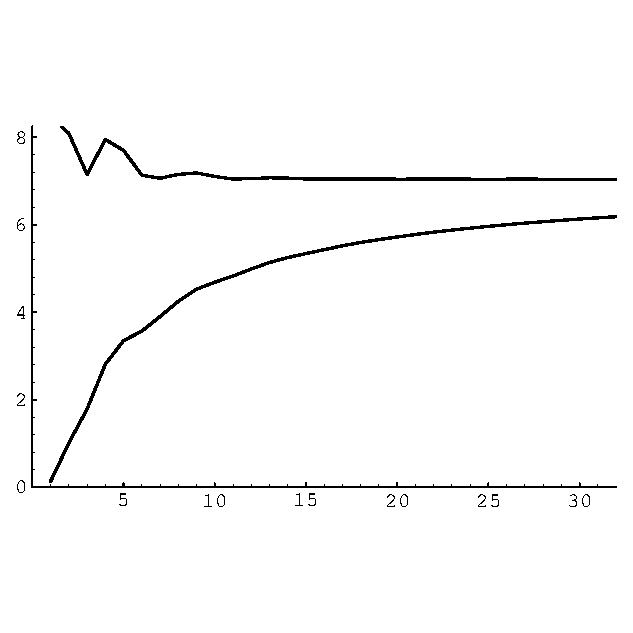
\includegraphics[width=3.25in]{graeffeb}
\end{center}
\caption{Upper and lower bounds on $M(P)$\label{Graeffe:Bound:Fig}}
\end{figure}

The lower bound of \propref{Graeffe:Bound:Prop} is not particularly
sharp, although the upper bound can be made quite sharp by increasing the
size of $k$.  

To illustrate this technique consider the following polynomial
suggested by \cite{Cerlienco1987-vl}
\[
P(X)  = X^6 + X^5 + 6X^4 - 5X^3 + 3X^2 + 2,
\]
which has zeroes
\[
-0.9015 \pm 2.4962 i, \quad0.6745 \pm 0.5646i, \quad
-0.2730 \pm 0.5408i.
\]
Only the first two zeroes are outside the unit circle and their
product is $7.0436280 = M(P)$.  \figref{Graeffe:Bound:Fig} shows the
upper and lower bounds on $M(P)$ based on $P_k$ as $k$ ranges from $1$
to $32$.  For $k = 11$ we already get the quite good upper bound of
$7.0470$, while the lower bound is $4.8284$.  For $k = 2048$, the
lower bound rises to $7.02934$, but computationally this is quite
expensive, due to the size of the coefficients of $P_m(X)$.

\section{Weighted Coefficient Bounds}
\label{Weighted:Bounds:Sec}


The relationship between $|p_i|$ and $M(P)$ given in
\eqnref{CoefZ:Bound:Eq} can be used to derive a bound on the
individual coefficients of divisors of a polynomial, as noted by
Mignotte \cite{Mignotte1974-oa}.  

\begin{proposition}[Mignotte]\label{Mignotte:Bound:Prop}
Let $Q(X) = q_0 X^{r} + q_{1} X^{r-1} + \cdots + q_{r}$ be a
polynomial over $\C$ that divides $P(X)$.  Then
\[
\left| q_{i} \right| \le \binom{r}{i} \left\|P\right\|.
\]
\end{proposition}
\begin{proof}
By \eqnref{CoefZ:Bound:Eq} we have,
\[
|q_i| \le \binom{r}{i} M(Q).
\]
Since every zero of $Q$ is a zero of $P$, we have $M(Q) \le M(P)$, and
by \propref{Landau:Zeroes:Prop}, $M(P) \le \|P\|$, which gives the
proposition. 
\end{proof}

This proposition indicates that the coefficients closer to the middle
of $Q(X)$ can be substantially larger than coefficients near the
leading and trailing terms.  Recently, this observation was made
substantially more precise by using the {\em weighted $L_2$ norm}.

Comparing the definition of the $[\cdot]_2$ norm \eqnref{PB:Beauzamy:Eq} 
with the lower inequality in \eqnref{CoefZ:Bound:Eq} we see that
\[
\sum_{0\le i \le d} \binom{d}{i}^{-1} |p_i|^2 \le
\sum_{0\le i \le d} \binom{d}{i} M^2(P).
\]
So, $[P]_2 \le 2^{d/2} M(P)$.  Applying the inequality to $M(P_1 P_2) = 
M(P_1) M(P_2)$, where $\deg P_1 + \deg P_2 = d$ gives:
\[
2^{d/2} \sqrt{d+1} |P_1 P_2| \ge [P_1]_2 \, [P_2]_2.
\]
More sophisticated techniques \cite{Beauzamy1990-yo} can be used to prove the 
following proposition.

\begin{proposition}
Let $f$ and $g$ be polynomials in one variable of degree $m$ and $n$
respectively.  Then
\[
[fg]_2 \ge \sqrt{\frac{m! \, n!}{(m+n)!}} [f]_2 \, [g]_2,
\]
and this result is best possible.
\end{proposition}

The following proposition \cite{Beauzamy1992-ts} is an analogue of 
\propref{Mignotte:Bound:Prop}, but uses the $[\cdot]_2$ norm. 

\begin{proposition} 
Let $P(X)$ be a univariate polynomial in $X$ over $\Z$, with
non-vanishing constant term.  Let $Q(X)$ be a divisor of $P(X)$, also
with rational integer coefficients.  Denote $\deg P$ by $d$, and $m =
\deg Q$.  Then each coefficient $q_i$ of
$Q(X)$ satisfies
\[
|q_i| \le \sqrt{\frac{1}{2} \binom{m}{i} \binom{d}{m}} [P]_2
   \le \sqrt{\frac{n!}{2(d-m)!\, (m-i)!\, i!}} [P]_2.
\]
Furthermore, 
\[
|Q| \le \frac{3^{3/4}}{2\sqrt{\pi}}\, \frac{3^{d/2}}{\sqrt{d}} [P]_2.
\]
\end{proposition}


\section{Size of a Polynomial's Zeroes}
\label{PB:RootSize:Sec}

The following inequality is due to {\Cauchy}
\cite{Cauchy1829-wp}.\Marginpar{Need intro}

\begin{proposition}[Cauchy]
\label{Cauchy:Zero:Bound:Prop}
Let $P(X) = X^{d} + p_{1} X^{d-1} + \cdots + p_{d}$ be a non-constant,
monic polynomial with coefficients in $\C$.  Then each root of $P(X)$,
$\alpha$, satisfies the inequality
\begin{equation}
\label{Cauchy:Zero:Ineq:Eq}
\left|\alpha\right| < 1 + \max \{|p_{1}|, \ldots, |p_{n}|\} 
  = 1 + \left| P \right|.
\end{equation}
\end{proposition}

\begin{proof}
Assume $|\alpha|$ is greater than $1$, otherwise the proposition is obvious.
By taking the absolute value of 
\[
\alpha^d = -(p_{1} \alpha^{d-1} + \cdots + p_{n}),
\]
we have
\[
\left| \alpha \right|^{d} = \left| p_{1} \alpha^{d-1} + \cdots + p_{n} \right|
 \le \left| \alpha^{d-1} + \cdots + 1 \right| |P| 
 \le { |\alpha|^{d} \over |\alpha| - 1} |P|.
\]
Since $|\alpha| > 1$, we can multiply by $|\alpha| - 1$ which gives 
$|\alpha| \le 1 + |P|$. 
\end{proof}

In \propref{Cauchy:Zero:Bound:Prop} we assumed that $P(X)$ is monic.  If this is not the case, we
can monicize the polynomial and apply \propref{Cauchy:Zero:Bound:Prop}.  In
particular, let 
\[
P(X) = p_{0} X^{d} + \cdots + p_{d},
\]
and let $\alpha$ be a zero of $P(X)$.  Applying the proposition to
\[
X^{d} + \frac{p_{1}}{p_{0}}X^{d-1} + \cdots + \frac{p_{d}}{p_{0}}
\]
gives
\[
\begin{aligned}
|\alpha| & 
   \le 1 + \max\{ \frac{p_{1}}{p_{0}}, \ldots, \frac{p_{d}}{p_{0}} \},\\
 & \le \frac{\left|p_{0}\right| + 
               \max \{\left|p_{1}\right|, \ldots, \left|p_{d}\right|
\}}{\left|p_{0}\right|}.
\end{aligned}
\]
Applying \propref{Cauchy:Zero:Bound:Prop} to the monic polynomial of
$1/\alpha$:
\[
X^{d} + \frac{p_{d-1}}{p_{d}} X^{d-1} + \cdots + \frac{p_{0}}{p_{d}}
\]
gives
\[
|\alpha| \ge \ \frac{\left|p_{d}\right|}{\left|p_{d}\right| + 
   \max\{ \left|p_{0}\right|, \ldots, \left|p_{d-1}\right|\}}.
\]
Putting these two results together we have for each zero of $P(X)$,
\[
\frac{\left|p_{0}\right| + 
               \max \{\left|p_{1}\right|, \ldots, \left|p_{d}\right|
\}}{\left|p_{0}\right|}
\ge
|\alpha| \ge \ \frac{\left|p_{d}\right|}{\left|p_{d}\right| + 
   \max\{ \left|p_{0}\right|, \ldots, \left|p_{d-1}\right|\}}.
\]

\section{Discriminants and Zero Separation}
\label{PB:RootSeparate:Sec}

This section obtains bounds on the minimum difference between zeroes of a
polynomial $P(X)$.  One of the most useful expressions involving the
difference of zeroes of $P(X)$ is the {\em discriminant} of $P$, which
is essentially the square of the product of differences of pairs of
zeroes of $P(X)$.  This quantity is quite useful in the study of
algebraic extensions.

\paragraph{Discriminants}

As usual, let $\alpha_1, \ldots, \alpha_d$ denote the zeroes of
$P(X)$.   Consider the \keyi{Vandermonde matrix}
\[
P_D = 
\left(\begin{array}{ccccc}
1 & \alpha_1 & \alpha_1^2 & \cdots & \alpha_1^{d-1} \\
1 & \alpha_2 & \alpha_2^2 & \cdots & \alpha_2^{d-1} \\
\vdots & & \vdots & \cdots & \vdots \\
1 & \alpha_d & \alpha_d^2 & \cdots & \alpha_d^{d-1} 
\end{array}\right),
\]
which is discussed in some detail in
\sectref{Vandermonde:Sec}.  Its determinant is equal to the product of
the difference of the zeroes of $P(X)$:
\[
\det P_D = \prod_{1\le i < j \le d} ( \alpha_i - \alpha_j).
\]
The {\em discriminant} of $P(X)$\index{discriminant!of a
polynomial} is defined to be
\addsymbol{$\protect\Dscr(P)$}{The discriminant of the polynomial $P$}
\begin{equation}\label{PB:Discriminant:Eq}
\Dscr(P) = p_0^{2d-2} \det|P_D|^2.
\end{equation}

The discriminant of a polynomial can be computed using
resultants.  We write $P(X)$ as
\[
P(X) = p_0 (X - \alpha_1) (X - \alpha_2) \cdots (X - \alpha_d).
\]
Its derivative is
\[
P'(X) = p_0(X - \alpha_2) \cdots (X - \alpha_d) + \cdots + p_0(X - \alpha_1) \cdots (X -
\alpha_{d-1}).
\]
Evaluating at $\alpha_i$ we have
\[
P'(\alpha_i) = p_0(\alpha_i - \alpha_1) \cdots \widehat{(\alpha_i -
\alpha_i)} \cdots (\alpha_i - \alpha_d),
\]
where the circumflex indicates a term in the product that is omitted.
Taking the product over all zeroes of $P(X)$ gives
\[
\begin{aligned}
P'(\alpha_1) \cdots P'(\alpha_d) 
  & \displaystyle
    = (-1)^{d(d-1)/2} p_0^d \prod_{1\le i< j \le n}(\alpha_i - \alpha_j)^2,\\
  & \displaystyle
    = (-1)^{d(d-1)/2} p_0^{2-d} \Dscr(P).
\end{aligned}
\]
By the definition of the resultant \eqnref{Resultant:Def:Eq} 
(page \pageref{Resultant:Def:Eq})
\[
\res_X (P(X), P'(X)) = p_0^{d-1}P'(\alpha_1) \cdots
P'(\alpha_d),
\]
since either $d$ or $d-1$ is even.  Combining these two equations gives
\[
\Dscr(P) = (-1)^{d(d-1)/2} \frac{\res_X (P(X), P'(X))}{p_0}.
\]

This formula allows us to compute the discriminant of specific
polynomials quite readily.  In particular,
\[
\begin{aligned}
\Dscr(aX^2 + bX + c) & = b^2 - 4ac, \\
\Dscr(X^3 + bX + c)  & = -(27 c^2 + 4b^3).
\end{aligned}
\]
For binomial polynomials we have,
\[
\begin{aligned}
\Dscr(X^n +a) &= (-1)^{n(n-1)/2} \res_X(X^n + a, n X^{n-1}), \\
 & = (-1)^{n(n-1)/2} \res_X(X^n + a, n) \res_X(X^n + a, X)^{n-1}, \\
 & = (-1)^{n(n-1)/2} n^n a^{n-1},
\end{aligned}
\]
where we have used \longpropref{Resultant:Properties:Prop}.

For trinomials the computation is a bit more difficult, but we do have
the following result of {\Swan} \cite{Swan1962-lf}.

\begin{proposition}[Swan]
Let $m$ and $n$ be positive integers with {\sc gcd} $d$ and cofactors
$M$ and $N$ respectively.  Then
\[
\begin{aligned}
\Dscr(X^m & + aX^n +b)\\
  & =
 (-1)^{m(m-1)/2} b^{n-1} (m^M b^{M - N} - (-1)^M (m - n)^{M - N} n^N a^M)^d.
\end{aligned}
\]
\end{proposition}
\begin{proof}
By the definition of the discriminant we have
\[
\Dscr(X^m + aX^n +b) 
    = (-1)^{m(m-1)/2} \res_X (X^m + aX^n + b, mX^{m-1} + anX^{n-1}).
\]
Since
\[
X^m + a X^n + b = \frac{X}{m} \cdot \left( mX^{m-1} + a n
X^{n-1}\right)
  + a \frac{m - n}{m} X^n + b,
\]
we have
\[
\begin{aligned}
\Dscr(X^m &+ aX^n +b) \\
  & = (-1)^{m(m-1)/2}  m^{m-n} \res_X (a \frac{m - n}{m} X^n + b, mX^{m-1} + anX^{n-1}).
\end{aligned}
\]
The resultant in this expression can be evaluated by factoring
\[
mX^{m-1} + a n X^{n-1} = X^{n-1} \times (m X^{m-n} + a n),
\]
and computing the two resultants:
\[
\res_X (a \frac{m - n}{m} X^n + b, X^{n-1}) = b^{n-1}
\]
and 
\[
\begin{aligned}
\res_X &(a \frac{m - n}{m} X^n + b, mX^{m-n} + an)\\
  &\qquad\qquad\qquad\qquad =
\left(b^{M-N} m^N - (-1)^N \left(a \frac{m-n}{m}\right)^{M-N} a^N
n^N\right)^d
\end{aligned}
\]
using \longpropref{Binomial:Result:Prop}.
When these results are multiplied and expanded we get the proposition.
\end{proof}

\medskip
Using \longpropref{Resultant:Bound:Prop} we can bound $|\Dscr(P)|$ as
\begin{equation}\label{PB:DiscrmBound1:Eq}
|\Dscr(P)| \le (\deg P + \deg P')! \,|P|^{d-1} |P'|^d \le (2d-1)! \,d^d\,
|P|^{2d-1}.
\end{equation}


This bound can be sharpened by applying the \key{Hadamard inequality}
(\longpropref{Hadamard:Ineq:Prop}) to $P_D$.  First, let $\alpha_i$ be a 
zero of $P(X)$ with absolute value less than $1$.  For each row
of $P_D$, we have
\[
\|\langle 1, \alpha_i, \ldots \alpha_i^{d-1} \rangle\|_2
\le \sqrt{1^2 + 1^2 + \cdots + 1^2} \le \sqrt{d}.
\]

Now, assume the zeroes of $P(X)$ satisfy
\[
|\alpha_1| \ge |\alpha_2| \ge \cdots \ge |\alpha_m| \ge 1 \ge |\alpha_{m+1}|
\ge \cdots \ge |\alpha_d|.
\]
So, the first $m$ zeroes of $P(X)$ lie outside the unit disk.
Dividing the first row by $\alpha_1^{d-1}$, the second row by
$\alpha_2^{d-1}$ and so on, we have
\[
Q_D = \frac{P_d}{(\alpha_1 \cdots \alpha_m)^{d-1}} =
\left(\begin{array}{ccccccc}
\alpha_1^{1-d} & \alpha_1^{2-d} & \alpha_1^{3-d} & \cdots & 1 \\
\vdots & & \vdots & \cdots & \vdots \\
\alpha_m^{1-d} & \alpha_m^{2-d} & \alpha_m^{3-d} & \cdots & 1 \\
1 & \alpha_{m+1} & \alpha_{m+1}^2 & \cdots & \alpha_{m+1}^{d-1} \\
\vdots & & \vdots & \cdots & \vdots \\
1 & \alpha_d & \alpha_d^2 & \cdots & \alpha_d^{d-1} 
\end{array}\right),
\]
where each element of $Q_D$ has absolute value less than $1$.  By
Hadamard's inequality, $\det|Q_D|$ can be bounded by $d^{d/2}$.
Thus,
\[
\det|P|= (\alpha_1 \cdots \alpha_m)^{d-1} \det|Q_D| \le 
\frac{M(P)^{d-1}}{p_0^{d-1}} d^{d/2},
\]
in general.  This immediately gives the following upper bound for the
discriminant. 

\begin{proposition}
If $P(X)$ is a univariate polynomial over $\C$ of degree $d$ and
leading coefficient $p_0$ then the absolute value of the discriminant
of $P(X)$ is bounded by
\[
|\Dscr(P)| \le d^d M(P)^{2(d-1)} \le d^d \|P\|^{2(d-1)}.
\]
\end{proposition}

The last inequality follows from \propref{Landau:Zeroes:Prop}.  Lower
bounds for the discriminant are much more subtle.  We quote the
following results of {\Odlyzko} in this regard \cite{Odlyzko1975-do,Odlyzko1977-rt}:

\begin{proposition}
Let $P(X)$ be a univariate, square free polynomial over $\Z$ of degree
$d$.  Denote the number of real zeroes of $P(X)$ by $r_1$ and the
number of complex zeroes by $2r_2$.  Then
\[
\begin{aligned}
|\Dscr(P)| & \ge (60.1)^{r_1} (22.2)^{2r_2} e^{-254}, \\
|\Dscr(P)| & \ge (58.6)^{r_1} (21.8)^{2r_2} e^{-70}. \\
\end{aligned}
\]
Assuming the generalized Riemann hypothesis
\[
|\Dscr(P)| \ge (188.3)^{r_1} (41.6)^{2r_2} e^{-3.7\times10^8}.
\]
\end{proposition}


\paragraph{Zero Separation}

In order to numerically determine the zeroes of $P(X)$, a univariate
polynomial of degree greater than $1$, it is important to know when
two zeroes are identical.  Since we cannot have exact finite numerical
representations of the zeroes of $P(X)$, we need a lower bound on how
close two distinct zeroes of a $P(X)$ can be.  We define the {\em zero
  separation}\index{zero separation} of $P$ to be
\[
\Delta(P) = \min_{i \not= j} \left| \alpha_{i} - \alpha_{j} \right|.
\]
\addsymbol{$\Delta(P)$}{minimum zero separation of two distinct zeroes
of the univariate polynomial $P$}

Assume that $|\alpha_i - \alpha_j|$ is the difference of roots of
$P(X)$, $i < j$.  We will use a slight variation of the techniques
used for discriminants to get an upper bound on $\det|P_D/(\alpha_i -
\alpha_j)|$.  This immediately yields a lower bound on $\Delta(P)$. 

Start with $P_D$ and subtract the $j$-th row from the $i$-th row,
\[
\left(\begin{array}{ccccccc}
1 & \alpha_1 & \alpha_1^2 & \cdots & \alpha_1^{d-1} \\
\vdots & & \vdots & \cdots & \vdots \\
0 & \alpha_i - \alpha_j & \alpha_i^2 - \alpha_j^2 & \cdots &
\alpha_i^{d-1} - \alpha_j^{d-1} \\
\vdots & & \vdots & \cdots & \vdots \\
1 & \alpha_d & \alpha_d^2 & \cdots & \alpha_d^{d-1} 
\end{array}\right).
\]
$\alpha_i - \alpha_j$ divides the $i-th$ row of this matrix so
\[
\frac{\det|P_D|}{\alpha_i - \alpha_j} = 
\left(\begin{array}{ccccccc}
1 & \alpha_1 & \alpha_1^2 & \cdots & \alpha_1^{d-1} \\
\vdots & & \vdots & \cdots & \vdots \\
0 & 1 & q_2 & \cdots & q_{d-1} \\
\vdots & & \vdots & \cdots & \vdots \\
1 & \alpha_d & \alpha_d^2 & \cdots & \alpha_d^{d-1} 
\end{array}\right),
\]
where 
\[
q_{\ell} = \alpha_i^{\ell-1} + \alpha_i^{\ell -2} \alpha_j + \cdots +
\alpha_j^{\ell-1}.
\]
We now divide the first $m$ rows by $\alpha_{\ell}^{d-1}$ as before.
The elements of all but the $i$-th row have absolute value no
greater than $1$.  The absolute values of the elements of the $i$-th
are bounded by $0, 1, 2, \ldots, {d-1}$ respectively, since
$|\alpha_i| > |\alpha_j|$.  

Applying Hadamard's inequality gives
\[
\frac{\det|P_D|}{(\alpha_i - \alpha_j) (\alpha_1 \ldots
\alpha_m)^{d-1}} 
\le d^{(d-1)/2}\sqrt{0^2 + 1^2 + \cdots + (d-1)^2}.
\]
The sum of squares inside the square root is easily bounded:
\[
0^2 + 1^2 + \cdots + (d-1)^2 = \frac{m(m-1)(2m-1)}{6} \le
\frac{m^3}{3}.
\]
Thus,
\[
\frac{p_0^{d-1} \det|P_D| \sqrt{3}}{M(P)^{d-1} d^{(d+2)/2}} 
   < |\alpha_i - \alpha_j|.
\]
Applying \eqnref{PB:Discriminant:Eq} gives {\Mahler}'s bound on the separation 
of the roots of $P(X)$ \cite{Mahler1964-vy}.

\begin{proposition}[{\Mahler}]
Let $p(x)$ be a square free polynomial of degree $d$ with discriminant $D$.
Then
\[
\Delta(p) > \sqrt{\frac{3 |D|}{d^{d+2}}} M(p)^{1-d}
\]
\end{proposition}

Using \propref{Landau:Zeroes:Prop} we have
\[
\Delta(p) > \sqrt{\frac{3 |D|}{d^{d+2}}} \|p\|^{1-d}.
\]

\section*{Notes}

\small

\notesectref{PB:Heights:Sec} Emma {\LehmerE} \cite{Lehmer1936-dj} surveyed
the early work on the size the coefficients in cyclotomic
polynomials. {\BatemanPT} gave an upper bound on the size of the
coefficients of a cyclotomic polynomial.  They are bounded above by
\[
\log A_n <  \frac{1}{2} d(n) \log n  
\le \frac{1}{2} \frac{(\log 2) (\log n)^2}{\log \log n},
\]
where $A_n$ is the absolute value of the largest coefficient in the
$n$-th cyclotomic polynomial.  Here we have used the bound
\eqnref{DivisorUBound:Eq} in the final inequality.  {\Vaughn}
\cite{Vaughan1974-vf} gave explicit lower bound,
\[
\log A_n > \exp \left( \frac{(\log 2) (\log n)}{\log \log n} \right),
\]
which implies both results are best possible.
{\Apostol} \cite{Apostol1975-js} contains a good bibliography of more
recent results.

\notesectref{Uniform:Bounds:Sec}  A nice proof of
\propref{Jensen:Formula:Prop} is contained in problems 120 and 175,
part III of P\'olya and Szeg\"o \cite{Polya1976-hx}.
{\Gelfond}'s proof of \propref{Factor:CBound:Prop}
\cite{Gelfond1960-ev} (pages 135--139) uses only elementary
techniques but it is quite a bit more lengthy than the one provided
here.

Mignotte \cite{Mignotte1992-sr} gives a bound similar to
\propref{Landau:Zeroes:Prop} but which uses a product of the $n$
largest roots, not all the roots. 

Alternative, more efficient approaches to the Graeffe method of
computing $M(P)$ are discussed in \cite{Cerlienco1987-vl}.  One interesting
observation that can be made from \figref{Graeffe:Bound:Fig} is that
the $\|P_k\|^{1/k}$ tends to be an especially good bound on $M(P)$
when $k$ is a prime number.  Can this statement be made more precise
and generalized?\Marginpar{Also checkout \cite{Boyd93a,Boyd93b,Mignotte94}.}

\notesectref{PB:RootSeparate:Sec} The presentation here follows that
of {\Mahler}'s original paper \cite{Mahler1964-vy}.
{\Mahler}'s proposition gives a lower bound on the separation of any pair 
of zeroes of a polynomial.  If a bound is only needed for a separation of 
real roots, then a bound of {\Rump} can be used that is a bit sharper 
\cite{Rump1979-dt}:
\[
\Delta_{real}(P) > \sqrt{\frac{8}{d^{d+2}}} \, \left(\frac{1}{1+|P|^d}\right).
\] 
\normalsize

%$Id: zero-test.tex,v 1.1 1992/05/10 19:35:22 rz Exp rz $
\chapter{Zero Equivalence Testing}
\label{Zero:Testing:Chap}

This chapter begins the discussion of ``modern'' algorithms that take
advantage of the sparsity of multivariate polynomials.  These
algorithms do not perform arithmetic operations with the polynomials
directly, but rather compute with the values of the polynomials at
selected points.  They produce the value of the final answer at these
points and then reconstruct the answer from the values.  This approach
eliminates \key{intermediate expression swell} and, when done
properly, only requires time polynomial in the size of the answer.
This is often called a \keyi{black box} model of computation since the
polynomials are treated as opaque boxes---how the values of the
polynomial are computed is not available to us.

In order to highlight the most important points this chapter
considers the simplest problem to which these methods
apply---determining when a polynomial is identically zero.  We call
this the \keyi{zero equivalence problem}.
\chapref{Interpolation:Chap} discusses interpolation schemes that
reconstitute univariate polynomials from their values and
\chapref{Sparse:Interp:Chap} discusses how this is done for
multivariate polynomials by taking sparsity into account.  In
\chapref{Poly:GCD:Chap} these methods are applied to the computation
of polynomial {\sc gcd}'s.  The discussion of the other major modern
scheme for dealing with sparsity begins with \chapref{Hensel:Chap}.

The study of large sparse problems is very much like the study of very
large physical objects (galaxies or black holes) or very small
physical objects (nuclear particles).  They are largely intractable,
and cannot be studied directly.  However, information about the
objects can be obtained indirectly, by their effect on other
computations.  Consider a situation where there is a quantity we wish
to study $P(X_1, \ldots, X_v)$, but where direct computation of $P$
is impractical.  By evaluating $P$ at certain points, we can still
study $P$ indirectly.

As an example of how this might arise, assume we are given $M$, a
square matrix over $\F_p[X_1, \ldots, X_v]$, with determinant $P(X_1,
\ldots, X_v)$.  How would we determine if $M$ is singular; \ie, if
$P$ is identically zero?  If $M$ is large (\eg, $100 \times 100$ with 
polynomial entries), explicitly computing $P$ is impractical due to
\key{intermediate expression swell}.  However, given elements of
$\F_p$, $a_1, \ldots, a_m$, it is relatively easy to determine $P(a_1,
\ldots, a_m)$, since it is an element of $\F_p$.  (We can compute the 
determinant of a $100\times 100$ matrix over a finite field directly using 
Gaussian elimination.)  Thus it is relatively easy to compute the values 
of $P$, but not $P$ itself.  The matrix $M$ can be viewed as a 
representation of a function that computes the value of $P$ at a point.

In this situation, we say that $P$ is represented by a \keyi{black
box} that returns the value of $P$ when given values for its
arguments.  When using a black box representation of a polynomial,
evaluation using the black box is the only way to inspect the
polynomial.  To be more precise, let $P(X_1, \ldots, X_v)$ be some
symbolic expression over a ring $R$.  ${\cal B}_P$ is a \keyi{black
box} representing $P$ if, for $x_1, \ldots, x_v \in \R$,  ${\cal
B}_P(x_1, \ldots, x_v)$ returns $P(x_1, \ldots, x_v)$.  Most often
$P(X_1, \ldots, X_v)$ is a polynomial, but rational and algebraic
functions are also possible.\Marginpar{This paragraph needs work.}

Let $\vec{a}$ be a $v$-tuple.  If ${\cal B}_P(\vec{a})$ is non-zero
then $P$ is not the zero polynomial.  However, the converse is not
true.  However unlikely, $\vec{a}$ may still accidently be chosen to
be a zero of $P$.  By quantifying the likeliness of accidently
choosing a zero of $P$, we can develop a {\em probabilistic}
algorithm for zero equivalence.  These techniques are discussed in
\sectref{Zero:Probabilistic:Sec}.

When we have a bound on the maximum number of non-zero terms in $P$,
the zero equivalence problem is called the {\em zero equivalence
problem with term bounds\/}.\index{zero equivalence problem! with term
bounds} This problem can be solved by deterministic algorithms that
take time polynomial in the size of $P$.  These techniques, which are
discussed in \sectref{Zero:Deterministic:Sec}, can be used to prove
that certain problems can be solved in polynomial time.  For most
practical problems, however, the probabilistic algorithms are more
useful.

Throughout this chapter and the next we assume polynomials are
represented in expanded form, as a list of monomials (pairs of
exponent-vectors and coefficients), and that monomials with zero
coefficients are omitted.  We denote the number of variables in a
polynomial by $v$, so the exponent vectors are $v$-tuples.  The
maximum degree of $X_i$ in $P$ is denoted by $d_i$ and the maximum of
the $d_i$ is denoted by $d$.  Occasionally, it is necessary to work
with polynomials for which we have \keyi{total degree bounds} instead
of individual degree bounds for each variable.  This bound is usually
given by $D$.  We always have
\[
d \le D \le vd.
\]

The number of non-zero monomials of the polynomial $P$ is usually
denoted by $t$ or $\terms P$.  The number of terms in a possibly
sparse polynomial is bounded by the number of terms in a dense
polynomial:
\[
\terms P \le (d+1)^v.
\]
Occasionally we will need to distinguish between the actual number of
terms in a polynomial and an {\em a priori} bound on the number of
terms in a polynomial.  We will use $T$ to denote the {\em a priori}
bound, and $t$ to denote the actual number of non-zero terms present
in $P$.
\addsymbol{$\terms P$}{The number of terms in the polynomial $P$}

There is a problem when analyzing the cost of algorithms that use
black boxes: How should we account for the cost of the black box
computation?  Different black boxes will require different amounts of
computation.  At best, we can parameterize this cost.  The most common
approach is merely to count the number of black box invocations.  For
example we might say that an algorithm requires ``$O(n^3)$ arithmetic
operations and invokes the black box $O(n)$ times.''  The second
approach is to assume that there is an exponent $\BBoxExp$ such
that the cost of a black box invocation on an input of size $w$ is
bounded by $O(w^{\BBoxExp})$.  With this convention, the cost of the
same algorithm might be $O(n^3 + n^{\BBoxExp})$.  If $\BBoxExp \le 3$,
then the resulting algorithm requires $O(n^3)$ operations. 


\section{Probabilistic Techniques}
\label{Zero:Probabilistic:Sec}

Without any bounds on the number of terms or the degree of the
variables in the polynomial $P$ and given only the black box ${\cal
B}_P$, one can provide substantial evidence that $P$ is the zero
polynomial by showing that ${\cal B}_P(\vec{a})$ returns zero for many
randomly chosen $v$-tuples $\vec{a}$.  In order to provide a
probabilistic algorithm for zero equivalence, we need to quantify how
strong this evidence actually is.

The only way that the evidence provided by ${\cal B}_P$ can be
misleading is if ${\cal B}_P$ returns $0$ when $P$ is actually
different from zero.  The following proposition quantifies how often
this can occur. It is the basis of nearly all the probabilistic
algorithms in computer algebra.

\begin{proposition}\label{Prob:Zero:Prop}
Let $A$ be an integral domain, $P$ a non-zero element of
$A[X_1,\ldots, X_v]$ and the degree of $P$ in each of $X_i$ be bounded
by $d_i$.  Let $Z_n(B)$ be the number of zeroes of $P$, $\vec{x}$ such
that $x_i$ is chosen from a set with $B$ elements, $B \gg d$.  Then
\[
\begin{aligned}
  Z_n(B) &\le B^v - (B-d_1)(B-d_2) \cdots (B-d_v)\\
    & \le (d_1 + d_2 + \cdots + d_v) B^{v-1}.
\end{aligned}
\]
\end{proposition}

\begin{proof}
There are at most $d_v$ values of $X_v$ at which $P$ is identically
zero.  So for any of these $d_v$ values of $X_v$ and any value for the
other $X_i$, $P$ is zero.  This comes to $d_vB^{v-1}$.  For all other
$B-d_v$ values of $X_v$ we have a polynomial in $v-1$ variables.  The
polynomial can have no more than $Z_{v-1}(B)$ zeroes.  Therefore,
\[
Z_v(B) \le d_v B^{v-1} + (B - d_v) Z_{v-1}(B).
\]

Rather than solving this recurrence for $Z_v$, we solve it for $N_v =
B^v - Z_v$.  Since $Z_1$ is less than or equal to $d_1$, $N_v \ge (B -
d_1)$.  This is the basis step of the inductive proof.  Writing the
recurrence in terms of $N_v$ we have
\[
B^v - N_v(B) \le d_v B^{v-1} + (B - d_v) (B^{v-1} - N_{v-1}(B))
\]
or
\[
N_v(B) \ge (B - d_v) N_{v-1}(B),
\]
from which the proposition follows. 
\end{proof}

The following polynomial actually has $B^v - (B-d_1) \cdots (B-d_v)$
zeroes with components less than $B$
\[
P(X_1, \ldots, X_v) =
\prod_{0 \le i_1 \le d_1}(X_1 - x_{1i}) \quad \cdots 
\prod_{0 \le i_v \le d_1}(X_v - x_{1v}).
\]
Thus the first inequality in the proposition cannot be further
strengthened.  

For the analysis of some algorithms the results of this theorem are
more useful when expressed in terms of probabilities.  We denote the
probability that $P$ is zero for $(x_1, \ldots, x_v)$, chosen randomly,
by
\[
{\cal P}(P(x_1, \ldots, x_v) = 0 \mid x_i \in {\cal S})
= \frac{Z_v(B)}{B^n} \le \frac{d_1 + \cdots d_v}{B}.
\]

Sometimes a similar bound is needed, but in terms of the total degree of
the polynomial $P$.\index{total degree, of a polynomial}  This bound
is provided by the following proposition.

\begin{proposition} \label{Prob:Total:Zero:Prop}
Let $P \in A[X_1, \ldots, X_v]$ be a polynomial of
total degree $D$ over an integral domain $A$.  Let ${\cal S}$ be a
subset of $A$ of cardinality $B$.  Then
\[
{\cal P}(P(x_1, \ldots, x_v)=0 \mid x_i \in {\cal S}) \le \frac{D}{B}.
\]
\end{proposition}

\begin{proof}
We use induction on the number of variables as was done in the proof
of the previous proposition.  For $v= 1$, $f$ is a univariate
polynomial of degree $D$ and can have no more than $D$ zeroes in $A$,
so 
\[
{\cal P}(P(x_1)=0 \mid x_1 \in {\cal S}) \le \frac{D}{B}.
\]

Assume the proposition is true for polynomials in $v-1$ variables.
Let the degree of $P$ in $X_v$ be $d_v$ and denote the leading
coefficient of $f$ with respect to $X_v$ by $f_0$, \ie,
\[
P = p_0(X_1, \ldots, X_{v-1}) X_v^d + \cdots.
\]
The total degree of $p_0$ is no more than $D - d$, so the probability
that $p_0 = 0$ is
\[
{\cal P}(p_0(x_1, \ldots, x_{v-1})=0 \mid x_i \in {\cal S}) \le \frac{D-d}{B}.
\]

Omitting the arguments of $x_1, \ldots, x_v$ and $x_1, \ldots,
x_{v-1}$ for brevity, we can write
\[
\begin{aligned}
{\cal P}(P =0) &= 
  {\cal P}(P =0 \wedge p_0=0) \cdot {\cal P}(p_0=0) \\
  & \qquad \qquad+
  {\cal P}(P=0 \wedge p_0\not=0) \cdot {\cal P}(p_0\not=0), \\
   & \le {\cal P}(p_0=0) + {\cal P}(P=0 \wedge p_0\not=0).
\end{aligned}
\]
Assume that $p_0(x_1, \ldots, x_{v-1})\not=0$. $P(x_1, \ldots,
x_{v-1}, X_v)$ is a polynomial of degree $d$, so there are at most $d$
$x_v \in {\cal S}$ such that $P(x_1, \ldots, x_v) = 0$. Consequently,
\[
{\cal P}(P(x_1, \ldots, x_{v})=0 \mid x_i \in {\cal S}) \le \frac{D -
d}{B} + \frac{d}{B} = \frac{D}{B}.
\]
\end{proof}


The following proposition phrases the result of
\propref{Prob:Zero:Prop} as a probability.

\begin{proposition} \label{Zero:MPoly:Prop}
Let $f_1, f_2, \ldots, f_s$ be elements of $A[X_1, \ldots, X_v]$, $A$
an integral domain, where the degree in each variable is bounded by
$d$.  Let ${\cal P}(f_1, \ldots, f_s)$ be the probability that a
randomly chosen point $\vec{x}$ is a zero of any of the $f_i$, where
$x_i$ is an element of a set with $B$ elements.  Then
\[
{\cal P}(f_1, \ldots, f_s) < \frac{vds}{B}.
\]
\end{proposition}

\begin{proof}
Let $f = f_1 f_2 \cdots f_s$.  The degree of each variable in $f$ is
bounded by $ds$.  Applying the previous proposition, we see that the
number of zeroes of $f$ is bounded by $vdsB^{v-1}$, for sufficiently
large $B$.  Since there are $B^v$ possible $\vec{x}$ from which to
choose, we have the corollary.
\end{proof}

\medskip
\propref{Zero:MPoly:Prop} gives a probabilistic algorithm for zero
equivalence.  We only indicate that a polynomial is non-zero when
${\cal B}_P$ returns a non-zero value, proving that $P$ is non-zero.
We want to know the probability that ${\cal B}_P$ returns zero even
though $P$ is not identically zero.  Assume that $P$ is not the zero
polynomial.

Define the set ${\cal S}_B$ to be
\[
{\cal S}_B = \{\,(x_1, \ldots, x_v) \mid 0 \le x_i < B\,\}.
\] 
Let $\vec{x}$ be an element of ${\cal S}_B$ such that ${\cal B}_P$
returns zero.  Then $\vec{x}$ is one of the at most $Z_v(B)$ zeroes in
of $P$ in ${\cal S}_B$.  If we choose $\vec{x}$ randomly, the
probability that we will get a zero of $P(\vec{X})$ is 
\[
{vD \over B},
\]
where the $D \ge \max(d_i)$.  The probability that $k$ randomly chosen
elements of ${\cal S}_B$ would all yield a value of zero (even though
$P$ is not the zero polynomial) is less than $(vD/B)^k$.

To verify that a polynomial $P(X_1, \ldots, X_v)$, whose degree in
each variable is less than $D$, is zero with probability less than
$\epsilon$ we need to perform $k$ evaluations with random elements of
${\cal S}_B$ where
\begin{equation}
\epsilon < \left({v D \over B}\right)^k. 
\label{Bound:Eq}
\end{equation}
A single evaluation will suffice if $B$ is chosen such that $B \ge
vD/\epsilon$.  The cost of the single evaluation is the cost of the
black box evaluation.  Recall that the cost of a black box evaluation
with $v$-tuple components of size $w$ is $O(w^{\BBoxExp})$, for some
$\BBoxExp$.  Since the size of the components of the random $v$-tuple is
$\log vD/\epsilon$, the cost of a single evaluation is
$O(\log^{\BBoxExp} v D/\epsilon)$.  If $k$ different evaluations are
used, then we need to choose $B$ such that \eqnref{Bound:Eq} is
satisfied.  So,
\[
\log B < \log vD + {1 \over k} \log {1 \over \epsilon}.
\]
The cost of a single evaluation when $k$ are intended is
\[
O\left(\log^{\BBoxExp} {vD \left({1 \over \epsilon}\right)^{1/k}}\right),
\]
and the total time required for $k$ evaluations using the
probabilistic approach will be 
\[
C_{\rm prob} 
   = O\left(k \log^{\BBoxExp} {vD \left({1 \over \epsilon}\right)^{1/k}}\right).
\]
This quantity is minimized when
\begin{equation}\label{Zero:PCount:Eq}
k = {({\BBoxExp} - 1) \log{1 \over \epsilon} \over \log vD}.
\end{equation}
Since $1/\epsilon \gg vD$, using multiple evaluations with relatively
small evaluation points is better than a single evaluation at a
large evaluation point. 

Replacing $k$ by this quantity in $C_{\rm prob}$ we have
\[
\begin{aligned}
C_{\rm prob} &= 
O\left({({\BBoxExp}-1) \log {1\over \epsilon} \over \log vD}
 \log^{\BBoxExp} {vD \left({1 \over
\epsilon}\right)^{ \log vD \over ({\BBoxExp}-1) \log {1\over \epsilon}}}\right)
\\
& = O\left({\log {1 \over \epsilon} \over \log vD} 
  \log^{\BBoxExp}  (vD)^{1+{1\over {\BBoxExp}-1}}\right)\\
& = O(\log {1 \over \epsilon} \times \log^{{\BBoxExp}-1} vD).
\end{aligned}
\]
Notice that the cost of the probabilistic algorithm is linear in the
logarithm of the error.  This is a good characterization of what it
means for a probabilistic algorithm to be polynomial time.

\medskip
Using the ideas in this section, the following routine
probabilistically checks to see if ${\cal B}_P$ represents a polynomial
that is identically zero.  The probability that this routine returns
an incorrect answer is controlled by the parameter $\epsilon$.  The
number of variables and the degree of the variables in $P$ is
indicated by $v$ and $D$ respectively.
\begindsacode
PZeroEquiv(${\cal B}_P$, $v$, $D$, $\epsilon$) := $\{$\\
\> $k \leftarrow  4 (\log 1/\epsilon)/(\log vD)$; \\
\> loo\=p for $0 \le i < k$ do \{ \\
\>\> if ${\cal B}_P(2^i, 3^i, \ldots, p_v^i) \not=0$ then return(false); \\
\>\> $\}$\\
\> return(true);\\
\> $\}$
\enddsacode

\noindent
Notice that in \keyw{PZeroEquiv} we have replaced $\BBoxExp - 1$ in
\eqnref{Zero:PCount:Eq} by $4$.  From a practical point of view this is
quite reasonable.  It is unlikely that the code in ${\cal B}_P$ would
have an exponent larger than $5$.

\section{Deterministic Results}
\label{Zero:Deterministic:Sec}

The probabilistic zero equivalence algorithm discussed in the previous
section is, from a practical point of view, quite sufficient.  However,
from a theoretical perspective it is desirable to know when the zero 
equivalence problem can be decided in \keyi{deterministic polynomial 
time}.  Given ${\cal B}_P$, a black box for the polynomial 
$P(X_1, \ldots, X_v)$ and degree bounds on $P$, only probabilistic 
algorithms are possible.  In essence this is because there are too many 
possible coefficients in $P$ and thus too many degrees of freedom to 
eliminate in polynomial time.  This is made more precise in 
\sectref{Zero:Negative:Sec}.  However, given a bound on the number of 
non-zero terms in $P$, there exist deterministic algorithms for zero 
equivalence. 

The first deterministic zero equivalence algorithm was
developed by {\Grigoriev} and {\Karpinski} \cite{Grigoriev87}.  It is
quite simple and does not even require degree bounds for the
polynomial---only a term bound.  However, this algorithm only works for 
polynomials over $\Z$ (though it is easily generalized to unique 
factorization domains).  The second algorithm, due to {\Zippel} 
\cite{Zippel90}, works over more general domains, but requires a degree 
bound in addition to the term bound. 

Assume we are given a black box for a polynomial, ${\cal B}_P$ and
want to determine if $P$ is identically zero.  The
only interaction the algorithm has with the black box is to pass it an
evaluation point and look at the result.  If the black box ever
returns a non-zero value, then $P$ is not identically zero and the
algorithm can terminate.  The sequence of test values used by the
algorithm cannot depend in any adaptive fashion on the responses from
${\cal B}_P$, since the responses will always be zero and thus do not depend
upon ${\cal B}_P$.  The sequence of test values {\em is} the
algorithm.  A sequence of test values that identifies the character of
a class of black boxes is called a \keyi{characterizing sequence}.  In
\sectref{Zero:Probabilistic:Sec} we proved that random sequences are
{\em likely} to characterize a black box, but this is not assured.

The two algorithms discussed here use different characterizing
sequences, but in both cases the sequences are based on the following 
proposition.

\begin{proposition}\label{Zero:Mon:Prop}
Let $P(\vec{X})$ be a non-zero polynomial in $R[\vec{X}]$ with at most
$T$ terms and with monomial exponent vectors $\vec{e}_i$.  Assume there
exists an $n$-tuple $\vec{x}$ (in some $R$-module) such that the
$\vec{x}^{\vec{e_i}}$ are distinct.  Then not all of $P(\vec{x}^0),
P(\vec{x}), P(\vec{x}^2), \ldots, P(\vec{x}^{T-1})$ are zero.
\end{proposition}

\begin{proof}
Denote $\vec{x}^{\vec{e}_i}$ by $m_i$.  By assumption, each of the
$m_i$ are distinct.  If $P$ vanished at each of the $\vec{x}^i$ then
the following system of linear equations would hold.
\[
\begin{aligned}
  c_1 + c_2 + \cdots + c_T &= 0 \\
  c_1 m_1 + c_2 m_2 + \cdots + c_T m_T &= 0\\
  c_1 m_1^2 + c_2 m_2^2 + \cdots + c_T m_T^2 &= 0\\ \vdots\\
  c_1 m_1^{T-1} + c_2 m_2^{T-1} + \cdots + c_{T} m_T^{T-1}&=0
\end{aligned}
\]
Since this is a Vandermonde system and we have assumed that the $m_i$
are distinct, the system of equations is non-singular.  Thus the $c_i$
must all be zero, and $P$ must be identically zero for all of
$P(\vec{x}^0), P(\vec{x}), P(\vec{x}^2), \ldots, P(\vec{x}^{T-1})$ to 
vanish.
\end{proof}


\paragraph{Without Degree Bounds}

The remaining problem is finding a substitution that keeps the
monomials distinct.  The technique of {\Grigoriev} and {\Karpinski} is
quite simple.  It is based on the observation that the rational
integers are a unique factorization domain. Thus if $p$ and $q$ are
\key{prime numbers} then $p^{e_1} q^{f_1}$ is equal to $p^{e_2} q^{f_2}$ if 
and only if $e_1= e_2$ and $f_1 = f_2$.  Since this keeps the terms 
distinct, by \propref{Zero:Mon:Prop}, it is a distinguishing set of 
evaluation points.  The following proposition makes this precise.

\begin{proposition}[{\Grigoriev} and {\Karpinski}]
\label{Deterministic:Zero:Prop}
Let $P(\vec{X})$ be a polynomial in $v$ variables over a ring of
characteristic zero, $A$, and assume that $P$ has no more than $T$
monomials.  Then there exists a set of $v$-tuples, $\{\vec{x}_0,
\ldots,
\vec{x}_{T-1}\}$ such that either $P(\vec{x}_i) \not= 0$ for some 
$\vec{x}_i$ or $P$ is identically zero.
\end{proposition}

\begin{proof}
Let $\vec{x} = (2, 3, 5, \ldots, p_v)$, where the entries are the 
canonical images of the prime numbers of $\Z$ in $A$.  By unique 
factorization of $\Z$, the monomials $\vec{x}^{\vec{e}_i}$ are distinct, 
and thus by \propref{Zero:Mon:Prop} either $P$ is identically zero or 
does not vanish at every element of the set $\{\vec{x}^0, \ldots,
\vec{x}^{T-1}\}$.
\end{proof} 

\propref{Deterministic:Zero:Prop} gives a simple deterministic
solution of the zero equivalence problem with term bounds.  We merely
pass each of the trial points $\vec{x}_0, \ldots, \vec{x}_{T-1}$ to ${\cal
B}_P$. If ${\cal B}_P$ returns an answer different from zero then $P$
is not the zero polynomial.  If ${\cal B}_P$ returns zero for all of
the trial points then it is the zero polynomial.
\begindsacode
GKZ\=eroEquiv(${\cal B}_P$, $n$, $T$) := $\{$\\
\> loo\=p for $0 \le i < T$ do \{ \\
\>\> if ${\cal B}_P(2^i, 3^i, \ldots, p_v^i) \not=0$ then return(false); \\
\>\> $\}$\\
\> return(true);\\
\> $\}$
\enddsacode

\keyw{GKZeroEquiv} requires $T$ evaluations using ${\cal B}_P$, the
last of which involves numbers as large $p_v^{T-1}$.  Since we have no
idea what computation is going on inside of ${\cal B}_P$ there is no
way to estimate the cost of each of the $T$ evaluations.  Thus the
most precise statement we can make about cost of {\tt GKZeroEquiv} is
that it requires $T$ evaluations and no other arithmetic operations.

Nonetheless, we can get some understanding of the \keyi{bit complexity} 
of using such 
large evaluation points by assuming that ${\cal B}_P$ simply
computes each of the monomials in $P$ and then adds up the values.  On
average, the $n$-th prime is no larger than $n \log n$ by the prime
number theorem.  So, the $k$-th evaluation by ${\cal B}_P$ will
require $O\left(M(k \log (n \log n))\right)$ time, where $M(K)$ is the
time to multiply two $K$ bit numbers.  For simplicity, we assume $M(K)
= K^2$.  Thus all $T$ evaluations require
\[
\sum_{k=0}^{T-1} O(k^2 \log^2 (v \log v))  = O(T^{3} \log^2 (v \log v))
\]
time.  Thus the complexity of \keyw{GKZeroEquiv} is dominated by the 
number of non-zero terms, not the degree of the polynomials.

The following proposition generalizes \propref{Deterministic:Zero:Prop} to 
the zero avoidance  problem for several polynomials.\Marginpar{Use development from lecture notes 4/18/95 for the following proposition.}

\begin{proposition}
\label{Interp:15:Prop}
Let $P_1(\vec{X}), \ldots, P_s(\vec{X}) \in A[X_1, \ldots, X_v]$ be
non-zero polynomials over a ring of characteristic zero, $A$, and
assume that 
\[
\terms P_1 + \cdots + \terms P_s = T.
\]
Let $\vec{x}$ be the image of $(2, \ldots, p_n)$ in $A^n$.  Then for some 
integer $j$, $0 \le j \le T$, all of $P_i(\vec{x}^j)$ are different from zero.
\end{proposition}

\begin{proof}
Denote the points $\{ \vec{x}^0, \vec{x}, \ldots, \vec{x}^T\}$ by
${\cal S}$.  $P_i$ cannot vanish at more than $\terms P_i$ elements of
${\cal S}$ by \propref{Deterministic:Zero:Prop}.\Marginpar{Do I need the generalized vanderonde results here? (prop. 114)}  Since ${\cal S}$
contains $T+1$ points, there must be one for which none of the $P_i$
vanish. 
\end{proof}

\paragraph{With Degree Bounds}

An alternate approach to the zero equivalence problem was developed 
independently by {\Grigoriev}, {\Karpinski} and {\Singer} 
\cite{Grigoriev90} and {\Zippel} \cite{Zippel90}.  The approaches in 
these two papers are almost 
identical, but with one slight variation that will be mentioned later.
The basic idea is that rather than showing that $P(\vec{X})$ is
non-zero, we choose a substitution $X_i \mapsto Z^{e_i}$ and show that
$P(Z^{\vec{e}})$ is non-zero.  This polynomial is univariate and has no
more non-zero terms than the original multivariate polynomial.
Proving that it is non-zero is relatively easy.

The crucial part of this technique is showing that the substitution
$\vec{X} \mapsto Z^{\vec{u}}$ does not send the non-zero polynomial
$P(\vec{X})$ to the zero polynomial, and furthermore that the degree
of $P(Z^{\vec{u}})$ is not too large.  To do this several different
substitutions are required.  All that we can prove is that if
$P(\vec{X})$ is not identically zero then one of the resulting
univariate polynomials will not be zero.

To illustrate the basic ideas, consider a simple version of this
technique that follows the approach used in the previous section.
Assume $R$ is a field, so $R[Z]$ is a unique factorization domain and
$Z+1, Z+2, \ldots$ are primes. Denote by $\vec{Z}$ the vector $(Z+1,
Z+2, \ldots, Z+v)$.  Thus the $\vec{Z}^{\vec{e}_i}$ are distinct.
Sending
\begin{equation}\label{Zero:LinearSubs:Eq}
(X_1, \ldots, X_v) \mapsto (Z+1, \ldots, Z+v) = \vec{Z}
\end{equation}
maps $P(\vec{X})$ into a univariate polynomial.  Since the $Z+i$ are
primes in a unique factorization domain, $\vec{Z}^0, \vec{Z}^1,
\ldots, \vec{Z}^{T-1}$ is characterizing sequence for any polynomial
$P$, with $T$ non-zero terms by \propref{Zero:Mon:Prop}.  In this
section we call the substitution of \eqnref{Zero:LinearSubs:Eq} a
\keyi{linear substitution}.

Unfortunately, this characterizing sequence yields a sequence of
univariate polynomials $P(\vec{Z}^i)$, each of whose degree is bounded
by $ivD$.  Since a univariate polynomial of degree $N$ cannot vanish
at more than $N$ values, each $P(\vec{Z}^i)$ can be characterized by
$ivD+1$ different values of $z$.  Combining these two steps gives the
following deterministic algorithm

\begindsacode
SD\=ZeroEquiv(${\cal B}_P$, $v$, $D$, $T$) := $\{$\\
\>loo\=p for $0 \le i < T$ do \{ \\
\>\> loo\=p for $0 \le z \le ivD$ do \{ \\
\>\>\> if \=${\cal B}_P((z+1)^i, (z+2)^i, \ldots, (z+v)^i) \not= 0$ \\
\>\>\>\>then return(false); \\
\>\>\> \}\\
\>\> \}\\
\> return(true); \\
\> \}
\enddsacode

\keyw{SDZeroEquiv} is a deterministic algorithm for zero equivalence,
but it requires that $R$ contain $vDT+1$ distinct elements if the
inner loop is modified appropriately.  When this is possible, it
generates a characterizing sequence of length $O(vDT^2)$.

When the coefficient field is contained in $\R$, we can improve the
number of evaluations required to characterize a univariate
polynomial.  The key is {\Descartes}' rule of signs:

\begin{proposition}[Descartes]
\label{Descartes:Sign:Prop}
Let $C$ denote the number of sign changes in the polynomial $p(x) \in
\R[x]$ and $Z$ the number of positive real zeroes.  Then $C - Z$ is a
non-negative even integer.
\end{proposition} 


Let $P(Z)$ be a univariate polynomial with $T$ non-zero
terms and denote the number of sign changes among its coefficients by
$C$.  Then $C$ is bounded above by $T-1$.  Applying
\propref{Descartes:Sign:Prop} gives 
\[
0 \le C - N_Z \le T - 1 - N_Z,
\]
which is stated as the following proposition.

\begin{proposition}
\label{Positive:Zeroes:Prop}
Let $P(x)$ be a univariate polynomial with coefficients in $\R$.  The
number of positive real zeroes of $P(x)$ is less than $\terms(P)$.
\end{proposition}

By choosing the evaluation points to be positive numbers the length of
the characterizing sequence for $P$ can be reduced from $\deg P$ to
$\terms P$, which can be much smaller.  The technique of {\tt
SDZeroEquiv} unfortunately, generates dense univariate polynomials.
By using a more sophisticated substitution we can reduce a
multivariate polynomial to a univariate polynomial that has no more
non-zero terms than the original multivariate polynomial.  This
technique will yield a characterizing sequence of length $O(vT^2)$ for
polynomials over $\R$.

\medskip
Instead of using the simple linear substitution of
\eqnref{Zero:LinearSubs:Eq}, we use:
\begin{equation} \label{Zero:MultiSub:Eq}
(X_1, X_2, \ldots, X_v) \longrightarrow
  (Z^{u_1}, Z^{u_2}, \ldots, Z^{u_v})
\end{equation}
where the $u_i$ are positive integers.  We call
\eqnref{Zero:MultiSub:Eq} a \keyi{nonlinear substitution}.  The
nonlinear substitution sends monomials in $P(\vec{X})$ to univariate
monomials in $Z$, so that $P(Z^{\vec{u}})$ has no more non-zero terms
than $P(\vec{X})$.  The difficulty is finding a vector $\vec{u}$ such
that $P(Z^{\vec{u}})$ is not identically zero.

The key idea is that the exponents $u_1, \ldots, u_v$ should come from a
large set of maximally independent $v$-tuples.

\begin{definition}
Let $\cal U$ be a set of $v$-tuples with components in $\Z$.
$\cal U$ is said to be \keyb{maximally independent} if every subset of
$v$ elements of $\cal U$ is $R$-linearly independent.
\end{definition}

In our situation, each element of $\cal U$, $\vec{u}$, corresponds to
a substitution $X_i \mapsto Z^{u_i}$.  If ${\cal U}$ is sufficiently
large, then some element $\vec{u} \in {\cal U}$ will lead to a
polynomial $P(Z^{\vec{u}})$ that is not identically zero.  The
following proposition shows that there exist arbitrarily large sets of
maximally independent $v$-tuples and that the components of the
$v$-tuples are not large.

\begin{proposition}
\label{SPMod:Lemma:1:Prop}
Let $S$ be a positive integer and $p$ be the smallest prime number
larger than $S$.  There exists a maximally independent set of $S$
$v$-tuples where each of the components of the $v$-tuples is less than
$p$.
\end{proposition}

\begin{proof}
First we show that we can construct arbitrarily large maximally
independent sets of $v$-tuples.  Then by reducing them modulo a prime
we get $v$-tuples of the size required by the proposition. Consider
$v$-tuples of the form $(1, k, k^2, \ldots, k^{v-1})$.  For $v$ of
these to be independent the determinant of the matrix
\[
\begin{pmatrix}
1& k_1 & k_1^2 & \cdots & k_1^{v-1}\\
1& k_2 & k_2^2 & \cdots & k_2^{v-1}\\
\vdots& &\vdots& & \vdots\\
1& k_v & k_v^2 & \cdots & k_v^{v-1}\end{pmatrix}
\]
must not be zero.  Since this is a \key{Vandermonde matrix}, it is
nonsingular if and only if the $k_i$ are different.  This and further
results on Vandermonde matrices are given in
\sectref{Vandermonde:Sec}.

Thus, if the $k_i$ are distinct then the vectors they generate will be
linearly independent.  In particular if we let $\vec{u}_k = (1, k,
\ldots, k^{v-1})$ then any subset of $n$ of the $\vec{u}_k$ will be
linearly independent.  Furthermore, if we reduce the elements of $\vec
u_k$ by $p$ the $k_i$ remain distinct modulo $p$ then the $v$-tuples
remain maximally independent.\Marginpar{This needs to be clarified a bit.}
\end{proof}

The size of the elements of the maximally independent set depend upon
the size of $p$.  By \key{Bertrand's postulate}
(\longpropref{Bertrands:Post:Prop}) there exists a $p$ greater than
$S$ and less than $2S$.  

In \cite{Grigoriev90} essentially identical techniques are used, but
the Vandermonde matrix used in the previous proposition is replaced by
the \keyi{Cauchy matrix} whose determinant is
\begin{equation}\label{Zero:Cauchy:Eq}
\det\left|
  \begin{array}{cccc}
\frac{1}{a_1+b_1} & \frac{1}{a_1+b_2} & \cdots & \frac{1}{a_1+b_v} \\[3pt]
\frac{1}{a_2+b_1} & \frac{1}{a_2+b_2} & \cdots & \frac{1}{a_2+b_v} \\[3pt]
\vdots & \vdots & & \vdots \\[3pt]
\frac{1}{a_v+b_1} & \frac{1}{a_v+b_2} & \cdots & \frac{1}{a_v+b_v} 
\end{array}\right|
=
\prod_{1\le i < j \le v}\frac{(a_j - a_i) (b_j - b_i)}{(a_i + b_j)}.
\end{equation}
As long as the $a_i$ and $b_j$ are (separately) distinct every square
submatrix of the Cauchy matrix will be non-singular and thus its rows will
be linearly independent.  Letting $a_i = 1, \ldots, S$ and $b_j = 1,
\ldots, v$ we get a sequence  of $S$ maximally independent vectors:
\[
(\frac{1}{2}, \frac{1}{3}, \ldots, \frac{1}{v+1}), 
(\frac{1}{3}, \frac{1}{4}, \ldots, \frac{1}{v+2}), \ldots
(\frac{1}{S+1}, \frac{1}{S+2}, \ldots, \frac{1}{S+v}).
\]
Again choosing a prime $p > S$ and reducing the components of each
vector by $p$ gives a sequence of vectors that satisfy
\propref{SPMod:Lemma:1:Prop}.  

For simplicity, we define ${\cal U}_{S,v}$ to be a set of maximally
independent $v$-tuples, where the components of each vector are
positive and less than $2S$.  Let $p$ be a prime such that $S < p
<2S$.  The previous discussion shows that either of the following
constructions of ${\cal U}_{S,v}$ can be used:
\[
{\cal U}_{S,v} =
\begin{array}{l}
  \{\, (1, i, i^2\mod p, \ldots, i^{v-1} \mod p) \mid 1 \le i \le v \,
\} \\[4pt]
  \{\, ((i+1)^{-1} \mod p, \ldots, (i+v)^{-1} \mod p) 
      \mid 1 \le i \le v \,\}
\end{array}
\]

\medskip
The following proposition uses the elements of the set ${\cal
U}_{nT,v}$ to construct univariate characterizing sequences for sparse 
polynomials.

\begin{proposition}\label{Sparse:ZeroPoly:Prop}
For every non-zero polynomial $P(X_1, \ldots, X_v)$ with no more than
$T$ non-zero terms and the degree of each $X_i$ bounded by $D$ there is a $\vec{u}$ in ${\cal U}_{vT,v}$ such that
$P(Z^{\vec{u}})$ is not identically zero.  Furthermore, the degree of
$P(Z^{\vec{u}})$ is less than $2v^2DT$ and $P(Z^{\vec{u}})$ has no
more than $T$ non-zero terms.
\end{proposition}

\begin{proof}
Let the non-zero terms of $P$ be
\[
P(\vec{X}) = c_1 \vec{X}^{\vec{e}_1} + c_2 \vec{X}^{\vec{e}_2} 
+ \cdots + c_T \vec{X}^{\vec{e}_T}.
\]
The substitution $X_i \mapsto Z^{u_i}$ transforms this polynomial into
\[
P(Z) = c_1 Z^{\vec{e}_1 \cdot \vec{u}} + c_2 Z^{\vec{e}_2 \cdot \vec{u}} +
\cdots +
c_T Z^{\vec{e}_T \cdot \vec{u}}.
\]
To find a substitution for which $P(Z^{\vec{u}})$ is not identically
zero we require $\vec{u}$ to satisfy
\[
\vec{e}_1 \cdot \vec{u} \not= \vec{e}_i \cdot \vec{u},
\]
or equivalently $(\vec{e}_i - \vec{e}_1) \cdot \vec{u} \not= 0$, for $2
\le i \le T$.  Let $d = \vec{e}_1 \cdot \vec{u}$.  With such a
substitution only the $c_1 \vec{X}^{\vec{e}_1}$ monomial of
$P(\vec{X})$ will be mapped to a term in $P(Z)$ of degree $d$.  Since
$c_1 \not= 0$, $P(Z)$ cannot be identically zero; it must contain a
$Z^d$ term.

Letting $L_i(\vec{w}) = (\vec{e}_i - \vec{e}_1)\cdot
\vec{w}$, $2 \le i < T$ we want to find a $\vec{w}$ at which none of
the $L_i$ vanish. 

Let $\vec{w}_1, \ldots, \vec{w}_v$ be distinct elements of ${\cal
U}_{vT, v}$, so
\[
\begin{pmatrix}\vec{w}_1 \\ \vdots \\ \vec{w}_v \end{pmatrix} \cdot
 (\vec{e}_i - \vec{e}_1)^T
 = 
\mathbf{A}\cdot (\vec{e}_i - \vec{e}_1)^T = 
  \begin{pmatrix}L_i(\vec{w}_1) \\ \vdots \\ L_i(\vec{w}_v) \end{pmatrix}.
\]
Since $\mathbf{A}$ is non-singular, the right hand side can only be zero
if $L_i$ is identically zero.  Thus, $L_i$ cannot vanish for more than
$n-1$ of the elements of ${\cal U}_{vT,v}$.  There are $T-1$ $L_i$'s.
Since $(v-1)\cdot (T-1)$ is less than $vT$, there must be at least one
element of ${\cal U}_{vT, v}$ for which none of the $L_i$ vanish as
desired.  We denote such an element by $\vec{u}$.  Each of the
components of $\vec{u}$ is less than $2nT$, while the elements of
$\vec{e}_i$ are less than $D$.  Thus the degree of $P(Z^{\vec{u}})$ is
less than $2v^2DT$.
\end{proof}

Using the univariate polynomial constructed in
\propref{Sparse:ZeroPoly:Prop} and the univariate polynomial zero test 
given by \propref{Positive:Zeroes:Prop}, we can construct the
following zero equivalence algorithm for black box polynomials over
the reals.

\begindsacode
RDZeroEquiv(${\cal B}_P$, $v$, $T$) := $\{$\\
\>loo\=p for $\vec{u} \in {\cal U}_{vT,v}$ do \{ \\
\>\> loo\=p for $1 \le z \le T$ do \{ \\
\>\>\> if \=${\cal B}_P(z^{u_1}, z^{u_2}, \ldots, z^{u_v}) \not= 0$ \\
\>\>\>\>then return(false); \\
\>\>\> \}\\
\>\> \}\\
\> return(true); \\
\> \}
\enddsacode

\begin{figure}
\begin{center}
\begin{tabular}{l|c|c|c|c|}
\multicolumn{1}{c}{} 
& \multicolumn{1}{c}{\# poly} & \multicolumn{1}{c}{\# terms} &
 \multicolumn{1}{c}{degree} & \multicolumn{1}{c}{\# points} \\ \cline{2-5}
Linear & $T$ & $\le vDT$ & $\le vDT$ & $vDT^2+T$ \\ \cline{2-5}
Nonlinear & $vT$ & $\le T$ & $\le v^2DT$ & $vT^2$ \\ \cline{2-5}
\end{tabular}
\end{center}
\caption{Complexity of different multivariate to univariate substitutions\label{Mult:Uni:Fig}}
\end{figure}

The table in \figref{Mult:Uni:Fig} illustrates the difference between
these two methods for black boxes over rings of characteristic zero.
Using the linear substitution \eqnref{Zero:LinearSubs:Eq} requires
generating $T$ polynomials of degree as large as $vDT$.  Since the
polynomials are dense the characterizing sequence of each must be of
length $vDT+1$ and the entire characterizing sequence for the black
box is of length $vDT^2+T$.  The non-linear substitution
\eqnref{Zero:MultiSub:Eq} produces more polynomials ($vT$) and
polynomials of greater degree, but each has no more than $T$ non-zero
terms.  By using positive integers as evaluation points, we get a
characterizing sequence of length $vT^2$.

\paragraph{Finite Fields}

If the characteristic of the coefficient domain is positive, then the
zero testing problem becomes a bit harder.  Consider, for instance,
the polynomial $M(X) = X^p - X$.  Even though $M(X)$ only has two
terms it vanishes for every element of $\F_p$.  Nonetheless,
\propref{Zero:Mon:Prop} is true for polynomial over fields of positive
characteristic.  The difficulty in this case is that there are no
values of $X$ that distinguish the two monomials of $M(X)$, $X^p$ and
$X$.  This problem does not arise for polynomials over fields of
characteristic zero, since there are many elements that distinguish
$X^m$ and $X^n$ when $m \not= n$.

This issue means that it is not possible to do {\em deterministic}
zero testing for polynomials over a finite field {\em without degree
bounds\/}.  However, the problem is solvable if we have degree bounds
on the black box.  

As usual, let ${\cal B}_Q$ be a black box for a polynomial $Q$.
Assume $Q$ is a univariate polynomial of degree $d$, with $T$ terms,
with coefficients in $\F_p$:
\[
Q(X) = q_1 X^{e_1} + q_2 X^{e_2} + \cdots + q_T X^{e_T},
\]
where $e_i \le d$.  Using \propref{Zero:Mon:Prop}, the sequence of
evaluation points, $1, m, m^2, \ldots$ will be a distinguishing
sequence if each of the values 
\[
m^{e_1}, m^{e_2}, \ldots, m^{e_T}
\]
are distinct. If the multiplicative order of $m$ is greater than $d$,
then these values are certainly distinct.

Now the problem is finding element of multiplicative order greater
than $d$.  In the case of $M(X) = X^p - X$, there is no such element
in $\F_p$ and thus there is no way to distinguish $M(X)$ from $0$
using a test sequence chosen from $\F_p$.  The solution to this
problem is to enlarge the ground field $\F_p$ to $\F_{p^k}$ which does
have elements of order $d$.  For instance, $\F_{p^2}$ has $\phi(p^2 -1)$
elements of order $p^2 -1$ any of which can be used to distinguish $M(X)$
from $0$.

In general there are three cases.  First, if the characteristic of the
ground field is very large, $p > 2^d$, then $m = 2$ will suffice.

Second, if $p$ is small we allow algorithms that are polynomial in
$p$.  The ground field $\F_p$, can be expanded by adjoining an element
of degree $k$ over $\F_p$, where $p^k > d$.  By
\propref{FF:AlgExtOrder:Prop} the field $\F_{p^k}$ has 
\[
\varphi(p^k -1) \approx \frac{6}{\pi^2} p^k -1
\]
elements of order $p^k -1$.  So with approximately $\lceil
\pi^2/6\rceil = 2$ random choices we should be able to find an
element of $\F_{p^k}$ whose multiplicative order is $p^k -1$.

Third, if $p$ is very large we cannot afford to find a multiplicative
generator of $\F_{p^k}$.  In this case we take the opposite approach,
and construct a very large degree extension of $\F_p$, one of degree
$K$ where $K > d$.  The generator of this extension will serve a good
generator for the irreducibility test.  
{\Adleman} and {\LenstraH} \cite{Adleman86} have shown that there
exists a positive integer $c$ such 
that using $(k \log p)^c$ steps one can find 
an irreducible polynomial of degree $d$ such that
\[
\frac{k}{c \log p} < d \le k.
\]
So, sufficiently large extensions can be found in polynomial
time.  %%\Marginpar{Needs work}

\section{Negative Results}
\label{Zero:Negative:Sec}

The zero equivalence problem with only degree bounds, and no bound on
the number of terms, is not solvable in deterministic polynomial time.
This is because it is too easy to find polynomials that vanish at a
large number of prescribed points and which still have small degree.
This is shown in the following proposition.

\begin{proposition}
\label{Key:Negative:Prop}
Let $D$, $T$ and $v$ be integers such that $D^v > T$.  Let ${\cal S} =
\{\vec{a}_i \}$ be a set of $T-1$ $v$-tuples.  There exists a
polynomial with rational integer coefficients with no more than $T$
non-zero monomials and that vanishes at each point in $\cal S$.
\end{proposition}

\begin{proof}
In fact, there are many polynomials that satisfy the requirements.
Choose a set of $T$ distinct $v$-tuples, $\vec{e}_1, \ldots, \vec{e}_T$,
where each component is an element of $\{0, 1, \ldots, D\}$.  The
polynomials with these exponents are all of the form 
\[
P(\vec{X}) = c_1 {\vec{X}}^{\vec{e}_1} + c_2 {\vec{X}}^{\vec{e}_2} 
+ \cdots + c_T {\vec{X}}^{\vec{e}_T}.
\]
We claim that at least one of these polynomials vanishes at each point
in ${\cal S}$.  For $P$ to vanish at $\vec{a}_i \in {\cal S}$ the $c_j$
must satisfy the following linear equation:
\[
c_1 {\vec{a}_i}^{\vec{e}_1} + c_2 {\vec{a}_i}^{\vec{e}_2} + \cdots +
c_T {\vec{a}_i}^{\vec{e}_T} = 0.
\]
Thus $P(\vec{X})$ vanishes at each element of $\cal S$ if the $c_j$
satisfy the following system of linear equations.
\[
\begin{aligned}
c_1 {\vec{a}_1}^{\vec{e}_1} + c_2 {\vec{a}_1}^{\vec{e}_2} + \cdots +
c_T {\vec{a}_1}^{\vec{e}_T} & = 0\\
c_1 {\vec{a}_2}^{\vec{e}_1} + c_2 {\vec{a}_2}^{\vec{e}_2} + \cdots +
c_T {\vec{a}_2}^{\vec{e}_T} & = 0\\
\vdots&\\
c_1 {\vec{a}_{T-1}}^{\vec{e}_1} + c_2 {\vec{a}_{T-1}}^{\vec{e}_2} 
+ \cdots +
c_T {\vec{a}_{T-1}}^{\vec{e}_T} & = 0
\end{aligned}
\]
Since these equations are homogeneous and there are more variables than
equations, the system possesses a non-trivial solution.
\end{proof}

\propref{Key:Negative:Prop} directly implies the non-existence of a
deterministic algorithm for zero recognition.

\begin{proposition}
\label{Black:Box:Prop}
Given a black box representing a polynomial $P(\vec{X})$ in $v$ variables
and of degree less than $D$ in each variable, any deterministic algorithm
that determines if $P$ is the zero polynomial runs in time at least
$O(D^v)$.
\end{proposition}

\begin{proof}
The time required by the algorithm is at least as large the number of
trial evaluations used.  Since no polynomial of degree less than $D$
has more than $D^v$ terms, $D^v$ trials suffice.  Thus the problem can
be solved in exponential time.  By \propref{Key:Negative:Prop}, if the
algorithm uses less than $D^v$ trials there will be polynomials that
meet the degree bounds and that are indistinguishable from the zero
polynomial.  Thus at least $D^v$ trial evaluations are required.
\end{proof}

Though the zero equivalence problem, given degree bounds, is not solvable
in deterministic polynomial time, notice that a polynomial that vanishes at
each of $O(D^v)$ trial points, constructed as in the proof of
\propref{Black:Box:Prop} would have $O(D^v)$ non-zero terms.  It would be
very interesting to know if there exists a polynomial that vanishes at
those trial points and that has a more succinct representation
(straight-line program, for instance).

\begin{figure}
{
\renewcommand{\arraystretch}{1.4}
\begin{center}
\begin{tabular}{l|c|c|}
\multicolumn{1}{c}{} & \multicolumn{1}{c}{Probabilistic}
   & \multicolumn{1}{c}{Deterministic}\\ 
\cline{2-3}
degree bounds & $\log {1 \over \epsilon} \times \log^{r-1} vD$ 
   & $D^v \log^r D$ \\ \cline{2-3}
term bounds & & $T^{r+1} \log^r v$ \\ \cline{2-3}
\end{tabular}
\end{center}
}
\caption{Complexity of Zero Testing\label{Zero:Comp:Fig}}
\end{figure}

The results of this section are summarized in the table in
\figref{Zero:Comp:Fig}.  The columns correspond to probabilistic and
deterministic algorithms respectively.  The rows correspond to whether
degree bounds or term bounds are given.  In the deterministic, bounded
degree case, we have given a lower bound on the time required, while
for the other two entries we have demonstrated algorithms that achieve
the indicated performance.  Also recall that $r$ is a constant
corresponding to the type of arithmetic being used by ${\cal B}_P$.
For classical arithmetic $r=2$; for fast arithmetic $r$ is slightly
greater than $1$.

As remarked earlier, the zero equivalence problem with degree bounds
cannot be solved in deterministic polynomial time, yet it can be
solved in probabilistic polynomial time.  We find it very curious that
with a slight change to the way information is provided, the problem
can be solved in deterministic polynomial time.  The zero equivalence
problem seems to lie on the boundary between those problems that can and
cannot be solved in deterministic polynomial time.  Though earlier
work has shown that random and deterministic polynomial time can be
separated via an oracle \cite{Heller86}, we find this example
interesting because it arises in a common practical problem.

By representing the polynomial as a black box, we have swept the issues of
the size of the computation required to compute $P(\vec{x})$ under the rug.
If we could look inside ${\cal B}_P$ and examine the ``program'' used to
compute $P(\vec{x})$ we might be able to show that ${\cal B}_P$ represents
the zero polynomial without any bounds on $P$.  For example, it seems
likely that one can prove that a straight-line program for a polynomial (in
the sense of {\Kaltofen} \cite{Kaltofen85d}) can be deterministically shown
to represent the zero polynomial in time polynomial in the size of the
straight-line program.



\section*{Notes}

\small

\notesectref{Zero:Probabilistic:Sec} The earliest mention of
probabilistic zero testing that we have been able to find appears in a
1978 note of {\DeMillo} and {\Lipton} on testing algebraic programs
\cite{Demillo78}.  They essentially reproduce \propref{Prob:Zero:Prop}.

Unaware of the prior work of {\DeMillo} and {\Lipton}, {\SchwartzJ}
\cite{Schwartz80} and {\Zippel} \cite{Zippel79a} simultaneously and
independently also proved \propref{Prob:Zero:Prop}.  (Apparently the time 
was ripe for this proposition.)  Their solutions to this problem were 
given in two successively presented papers at the EUROSAM '79 
conference in Marseille during the summer of 1979.  The slightly weaker 
result of the last line of the proposition was proven and used in the 
work of {\SchwartzJ} \cite{Schwartz80}, while that of the first line was 
given by  {\Zippel} \cite{Zippel79a}.

\notesectref{Zero:Deterministic:Sec}
The probabilistic techniques discussed in
\sectref{Zero:Probabilistic:Sec} were a dramatic improvement to the
state of the art in symbolic computation when they were introduced in
1979.  From the theoretical perspective, the work in
\cite{Zippel79b} essentially reduced a number of problems
(polynomial greatest common divisor and polynomial factorization) to
random polynomial time.  Moreover, the reduction led to algorithms
that were more efficient than the existing algorithms.  

For several years, it was believed that these problems were
intrinsically harder than deterministic polynomial time. In
particular, it was believed the zero equivalence problem could not be
solved in deterministic polynomial time.  The results of
\sectref{Zero:Negative:Sec}, which were well understood during the
1980's reinforced this belief.

In 1987 {\Grigoriev} and {\Karpinski}, as part of their work on
bipartite graph matching \cite{Grigoriev87}, developed a deterministic
algorithm for the zero equivalence problem for polynomials with
integer coefficients given a bound on the number of {\em non-zero
terms}.  These ideas where then used by {\BenOr} and {\Tiwari} in 1988
\cite{BenOr88} to produce a deterministic algorithm for interpolation
of sparse polynomials, which is discussed in
\sectref{Interp:BenOr:Sec}.  In 1988, {\Zippel} independently
developed a deterministic algorithm for the zero equivalence problem
with term bounds \cite{Zippel90} (as well as an interpolation
algorithm), which did not have the restrictions of {\Grigoriev} and
{\Karpinski} algorithm.

{\Risler} and {\Ronga} \cite{Risler90} independently developed an
approach similar to that of \cite{Zippel90,Grigoriev90}.

Building on \cite{Heintz80a}, {\Heintz} and {\Schnorr}
\cite{Heintz82a} have shown that there exist short characterizing
sequences for polynomials expressed as straight line programs.
Unfortunately, their techniques do not provide a way to generate these
characterizing sequences.  Determining these sequences is currently
the most important outstanding problem in zero testing.

\normalsize

%$Id: interp.tex,v 1.1 1992/05/10 19:42:22 rz Exp rz $
\chapter{Univariate Interpolation}
\label{Interpolation:Chap}

The previous chapter showed how to determine if a polynomial was zero
by examining its values at well chosen points.  This chapter develops
techniques to determine the polynomial itself from a sequence of 
values.  This process is called {\em interpolating a polynomial
from its values\/}.  This technique is one of the most useful tools
for constructing efficient symbolic computing algorithms for sparse problems.

In the previous chapter we used knowledge about when Vandermonde matrices
were non-singular to develop deterministic algorithms for zero
testing.  In this chapter we will also need to solve systems of
linear equations whose coefficients form a Vandermonde matrix.
\sectref{Vandermonde:Sec} develops some properties of Vandermonde
matrices and the basic techniques for dealing with Vandermonde style
systems of equations.

We consider two interpolation schemes for univariate polynomials in
the chapter, the \keyi{Lagrange interpolation formula} and the
\keyi{Newton interpolation formula}.  The Lagrange technique follows
directly from Vandermonde techniques discussed in
\sectref{Vandermonde:Sec} and are discussed in
\sectref{Interp:Lagrange:Sec}.  The Newton interpolation scheme arises 
from applying the Chinese remainder algorithm\index{Chinese remainder
theorem} to the values of a polynomial.  It is discussed in
\sectref{Interp:CRA:Sec}.

By choosing the evaluation points in an interpolation scheme
especially carefully, it is possible to interpolate exceedingly
quickly.  This technique, the \key{fast Fourier transform}, is
discussed in \sectref{Poly:FFT:Sec} and is applied to multiplying
polynomials.  This produces the fastest known polynomial multiplication
algorithm.  The complexities of these different algorithms is
summarized in \figref{Interp:Complex:Fig}.

\begin{figure}
\begin{center}
\begin{tabular}{|c|c|c|}
\multicolumn{1}{c}{Algorithm} & \multicolumn{1}{c}{Time} 
  & \multicolumn{1}{c}{Space} \\ \hline
Lagrange & $O(n^2)$ & $O(n)$ \\ \hline
Newton & $O(n^2)$ & $O(n)$ \\ \hline
Fast Fourier  & $O(n \log n)$ & $O(n)$ \\ \hline
\end{tabular}
\end{center}
\caption{Complexity of different interpolation
algorithms\label{Interp:Complex:Fig}}
\end{figure}


In \sectref{Interp:Abstract:Sec} we discuss interpolation from a
somewhat more abstract perspective.  This approach allows us to
combine the Chinese remainder theorem results for integers with those
for polynomials into a single uniform framework.

\section{Vandermonde Matrices}
\label{Vandermonde:Sec}

\index{Vandermonde matrix|(}

Vandermonde matrices have two properties that make them particularly
useful for the algorithms in this chapter: (1) it is easy to ensure
that they are non-singular and (2) systems of linear equations whose
coefficients form Vandermonde matrices are easy to solve exactly. Note
that Vandermonde matrices of floating point numbers can be numerically
quite unstable and these techniques may not be appropriate.

A \keyi{Vandermonde matrix} is a matrix of the form  
\begin{equation} \label{Vandermonde:Eq}
V_n = \begin{pmatrix}
1& k_1 & k_1^2 & \cdots & k_1^{n-1}\\
1& k_2 & k_2^2 & \cdots & k_2^{n-1}\\
\vdots& &\vdots& & \vdots\\
1& k_n & k_n^2 & \cdots & k_n^{n-1}\end{pmatrix},
\end{equation}
where the $k_i$ are chosen from some field.
Similarly, a system of linear equations of the form
\[
\begin{aligned}
X_1 + k_1 X_2 + k_1^2 X_3 + \cdots + k_1^{n-1} X_n &= w_1 \\
X_1 + k_2 X_2 + k_2^2 X_3 + \cdots + k_2^{n-1} X_n &= w_2 \\
\vdots&\\
X_1 + k_n X_2 + k_n^2 X_3 + \cdots + k_n^{n-1} X_n &= w_n 
\end{aligned}
\]
will be called a \keyi{Vandermonde system of equations}.

A matrix where the degrees of each column are the same and within each
row the degrees rise monotonically, is called a {\em generalized
Vandermonde matrix\/},\index{Vandermonde matrix!generalized} \viz,
\[
\begin{pmatrix}
k_1^{e_1}& k_1^{e_2} & k_1^{e_3} & \cdots & k_1^{e_n}\\
k_2^{e_1}& k_2^{e_2} & k_2^{e_3} & \cdots & k_2^{e_n}\\
\vdots& &\vdots& & \vdots\\
k_n^{e_1}& k_n^{e_2} & k_n^{e_3} & \cdots & k_n^{e_n}\end{pmatrix},
\]
where $e_1 < e_2 < \cdots e_n$.  We will often use generalized
Vandermonde matrices where $e_1 = 0$.

The determinant of a \key{Vandermonde matrix} is particularly simple
to compute.  Multiplying the $i$-th column of
\eqnref{Vandermonde:Eq} by $k_1$ and subtracting it from the
$i+1${\st} column gives,
\[
\det V_n = 
  \left|
  \begin{array}{ccccc}
    1&0&0 &\cdots &0\\
    1&k_2 - k_1&k_2^2 -k_1 k_2& \cdots &k_2^{n-1} - k_2^{n-2} k_1 \\
    \vdots&\vdots&\vdots&  & \vdots\\
    1&k_n - k_1&k_n^2 -k_1 k_n& \cdots &k_n^{n-1} - k_n^{n-2} k_1 
  \end{array}\right|.
\]
Expanding by \keyi{Cramer's rule} across the first row and factoring out
$k_i-k_1$ from the $i$-th row we have the following recursive
formula
\[
\begin{aligned}
\det V_n &= \det V_{n-1} \prod_{1<j \le n} \left(k_j - k_1\right), \\
  & = \det V_{n-2} \prod_{2<j \le n} \left(k_j - k_2\right) 
      \prod_{1<j \le n} \left(k_j - k_1\right).
\end{aligned}   
\]
Thus we have:

\begin{proposition}
The determinant of the \key{Vandermonde matrix} is
\[
\det V_n = \prod_{1 \le i < j \le n} \left(k_j - k_i\right).
\]
\end{proposition}

\noindent
As an immediate consequence, the determinant of a \key{Vandermonde matrix}
is non-zero if and only if the $k_i$ are distinct.

\medskip
This result is not true for generalized Vandermonde matrices.  For
instance, for order $2$ matrices we have 
\[
\det V_{2} = 
\left|
\begin{array}{cc}
 1&k_1^e \\ 1 &k_2^e
\end{array}\right| = k_2^e - k_1^e,
\]
which implies that $V_{2}$ is nonsingular if and only if $k_{1}/k_{2}$
is not an $e$-th root of unity.  This is a stronger requirement
than was required for Vandermonde determinants.  In fact, an $n
\times n$ generalized Vandermonde determinant is divisible by the
related Vandermonde determinant.  

Nonetheless, a similar result on the singularity of generalized
Vandermonde matrices over the {\em reals\/}
is true, but the proof is a little trickier.  The following
proposition is only valid over $\R$, which has characteristic zero.
We know of no similar result for fields of positive characteristic.
        
\begin{proposition}
\label{Gen:Vandermonde:Prop}
The determinant of a generalized Vandermonde matrix is non-zero if the
$k_i$ are distinct positive real numbers.
\end{proposition}

\begin{proof}
We show the matrix is non-singular by induction.  A Vandermonde matrix
of order 1 is obviously non-singular since we only allow positive entries.
In the general case we consider a matrix of the form
\[
\begin{pmatrix}
1& k_1^{e_2} & k_1^{e_3} & \cdots & k_1^{e_n}\\
1& k_2^{e_2} & k_2^{e_3} & \cdots & k_2^{e_n}\\
\vdots& &\vdots & & \vdots\\
1& k_n^{e_2} & k_n^{e_3} & \cdots & k_n^{e_n}
\end{pmatrix}.
\]
Replace $k_1$ by the indeterminate $Z$ and consider the number of zeroes of
the polynomial
\[
G(Z) = 
\left|\begin{array}{ccccc}
  1& Z^{e_2} & Z^{e_3} & \cdots & Z^{e_n}\\
  1& k_2^{e_2} & k_2^{e_3} & \cdots & k_2^{e_n}\\
  \vdots& &\vdots & &\vdots\\
  1& k_n^{e_2} & k_n^{e_3} & \cdots & k_n^{e_n}
\end{array}\right| =
a_1 - a_2 Z^{e_2} + a_3 Z^{e_3} - \cdots - a_n Z^{e_n}.
\]
Each coefficient ($a_i$) is a minor of the original matrix and is itself a\Marginpar{This paragraph needs to be fixed up.}
generalized Vandermonde matrix of order $n-1$.  If $k_2, k_3, \ldots , k_n$
are distinct positive numbers then the minors are non-zero by induction.
The polynomial in $Z$ can only have $n-1$ positive zeroes by
\longpropref{Positive:Zeroes:Prop}.  But certainly each of $k_2, k_3, \ldots,
k_n$ is a zero of the polynomial.  Thus there are no other positive
real zeroes and $G(k_1) \not= 0$.
\end{proof}

The inverse of a \key{Vandermonde matrix} can be computed by the
following technique.  Multiply a Vandermonde matrix by a general $n$
by $n$ matrix:
\begin{equation}\label{Vander:InvProd:Eq}
\begin{pmatrix}
1&k_1&k_1^2&\cdots&k_1^{n-1}\\
1&k_2&k_2^2&\cdots&k_2^{n-1}\\
\vdots& & \vdots& & \vdots\\
1&k_n&k_n^2&\cdots&k_n^{n-1}
\end{pmatrix} \cdot
\begin{pmatrix}
p_{11}&p_{12}&p_{13}&\cdots&p_{1n}\\
p_{21}&p_{22}&p_{23}&\cdots&p_{2n}\\
\vdots& & \vdots& &\vdots\\
p_{n1}&p_{n2}&p_{n3}&\cdots&p_{nn}
\end{pmatrix},
\end{equation}
where the $p_{ij}$ are chosen such that this product is equal to the
identity matrix.
The $j$-th element of the top row of the product of these two matrices is
\[
p_{1j} + p_{2j} k_1 + p_{3j} k_1^2 + \cdots + p_{nj} k_1^{n-1} = P_j(k_1),
\]
where $P_j(Z)$ is a polynomial of degree $n-1$ in $Z$.
So, the product \eqnref{Vander:InvProd:Eq} is equal to 
\[
\begin{pmatrix}P_1(k_1)& P_2(k_1) & \cdots & P_n(k_1)\\
P_1(k_2)& P_2(k_2) & \cdots & P_n(k_2)\\
\vdots & \vdots & & \vdots\\
P_1(k_n)& P_2(k_n) & \cdots & P_n(k_n)\end{pmatrix}.
\]
By choosing $P_i(Z)$ such that $P_i(k_j) = 0$ if $i\not= j$ and
$P_i(k_i) =1$ otherwise, the above matrix becomes the identity matrix.
We let $P_j(Z)$ be
\begin{equation} \label{Vander:Pj:Eq}
P_j(Z) = \prod_{\genfrac{}{}{0pt}{2}{i \not= k}{1 \le i \le n}}
  {Z - k_i \over k_j - k_i}.
\end{equation}
The numerator ensures that the off diagonal entries are zero, while
the denominator term ensures that the diagonal terms are one.

\medskip
We demonstrate these ideas by giving an algorithm for solving the following
Vandermonde system of equations: 
\begin{equation}\label{VandermondeSys:Eq}
\begin{aligned}
x_1 + k_1 x_2 + k_1^2 x_3 + \cdots + k_1^{n-1} x_n & = w_1,\\
x_1 + k_2 x_2 + k_2^2 x_3 + \cdots + k_2^{n-1} x_n & = w_2,\\
\vdots\\
x_1 + k_n x_2 + k_n^2 x_3 + \cdots + k_n^{n-1} x_n & = w_n.
\end{aligned}
\end{equation}
When recognized as a Vandermonde system, these equations need only
consume $O(n)$ space since only $k_1, \ldots, k_n$ and $w_1, \ldots,
w_n$ must be stored.  They can be solved using $O(n)$ space as
follows:

Let $\vec{x}$ be the column vector of unknowns $(x_1, \ldots, x_n)^T$
and $\vec{w} = (w_1, \ldots, w_n)^T$.  Then \eqnref{VandermondeSys:Eq}
can be written as
\[
V_n \cdot \vec{x} = \vec{w}.
\]
This equation is solved by multiplying on the left by the inverse of $V_n$:
\[
\left(
\begin{array}{c} x_1 \\ x_2 \\ \vdots \\ x_n \end{array}
\right) =
\left(
 \begin{array}{ccccc}
    p_{11}&p_{12}&p_{13}&\cdots&p_{1n}\\
    p_{21}&p_{22}&p_{23}&\cdots&p_{2n}\\
    \vdots& & \vdots& &\vdots\\
    p_{n1}&p_{n2}&p_{n3}&\cdots&p_{nn}
 \end{array}\right)
\cdot
\left(
\begin{array}{c} w_1 \\ w_2 \\ \vdots \\ w_n \end{array}
\right).
\]
So,
\begin{equation} \label{VanderSol:Eq}
\begin{aligned}
x_i & = p_{i1} w_1 + p_{i2} w_2 + \cdots + p_{in} w_n, \\
     &= \coef(P_1(Z), Z^{i-1}) w_1 + \cdots
       + \coef(P_n(Z), Z^{i-1}) w_n.
\end{aligned}
\end{equation}

This computation can be made quite efficient.  Define the {\em master 
polynomial} 
\begin{equation}
P(Z) = \prod_{1\le i \le n} \left(Z - k_i\right).
\label{Big:Poly:Eq}
\end{equation}
This polynomial contains $n+1$ terms.  The coefficient of $Z^n$ is
always $1$.  Expanding the product in \eqnref{Big:Poly:Eq}
requires $\Theta(n^2)$ arithmetic operations.  

Once $P(Z)$ is known each of the $P_j(Z)$ can be computed
in $O(n^2)$ arithmetic operations.  The numerator of $P_j(Z)$, which
is $P(Z)/(Z - k_j)$, can be computed by classical polynomial division
in $O(n)$ time.  The denominator of $P_j(Z)$, which is the value of
$P(Z)/(Z-k_j)$ at $Z = k_j$, can be computed in $O(n)$ time by
Horner's rule (\sectref{Poly:Subs:Sec}).  Thus each of the $P_j(Z)$
can be computed using $O(n)$ space and time.

The computation of the $x_i$ is arranged as follows.
\[
\begin{pmatrix}x_1\\ \vdots\\ x_n\end{pmatrix} =
\begin{pmatrix}w_1 \cdot \coef(P_1, Z^0) \\  \vdots \\ w_1 \cdot \coef(P_1, Z^{n-1}) \end{pmatrix}
+ \cdots +
\begin{pmatrix}w_n \cdot \coef(P_n, Z^0) \\  \vdots \\ 
         w_n \cdot \coef(P_n, Z^{n-1}) \end{pmatrix}.
\]
After each column vector on the right hand side is computed, it is 
added to the accumulating $X_i$ and its storage may be reused by 
the following column vector.  This approach leads to the following
program:
\begindsacode
SolveVandermonde (k[n], w[n]) := $\{$ \\
\> $Q(Z) \leftarrow   (Z - \mbox{k[$1$]})\times \cdots \times (Z - \mbox{k[$n$]})$; \\
\> $\mbox{x[$\cdot$]} \leftarrow 0$; \\
\> loo\=p for \=$1 \le i \le n$ do \{ \\
\>\> $Q_i(Z) \leftarrow \mbox{PolyQuotient}(Q(Z), Z - \mbox{k[$i$]})$; \\
\>\> $P_i(Z) \leftarrow Q_i(Z)/Q_i(k[$i$])$; \\
\>\> loo\=p for $1 \le j \le n$ do \{ \\
\>\>\> $\mbox{x[$j$]} \leftarrow \mbox{x[$j$]} + \mbox{w[$i$]} \cdot
\coef(P_i(Z), Z^{j-1})$;\\
\>\>\> $\}$ \\
\>\> $\}$ \\
\> return(x); \\
\> $\}$
\enddsacode

As pointed out above, the computation of each $P_i(Z)$ takes $O(n)$
arithmetic operations, so the time complexity of
\keyw{SolveVandermonde} is $O(n^2)$ and only $O(n)$ space is
required.

\medskip
This approach can also be applied to transposed Vandermonde
systems:\index{Vandermonde system!transposed}
\begin{equation}\label{Trans:Vander:Eq}
\begin{aligned}
x_1 + x_2 + x_3 + \cdots + x_n & = w_1,\\
k_1 x_1 + k_2 x_2 + k_3 x_3 + \cdots + k_n x_n & = w_2,\\
\vdots\\
k_1^{n-1} x_1 + k_2^{n-1} x_2 + k_3^{n-1} x_3 +
 \cdots + k_n^{n-1} x_n & = w_n.
\end{aligned}
\end{equation}

Since the inverse of the transpose of a matrix is the transpose of the
inverse, we have the following solution for $\vec{x}$
\[
\left(
\begin{array}{c} x_1 \\ x_2 \\ \vdots \\ x_n \end{array}
\right) =
\left(
 \begin{array}{ccccc}
    p_{11}&p_{21}&p_{31}&\cdots&p_{n1}\\
    p_{12}&p_{22}&p_{32}&\cdots&p_{n2}\\
    \vdots& & \vdots& &\vdots\\
    p_{1n}&p_{2n}&p_{3n}&\cdots&p_{nn}
 \end{array}\right)
\cdot
\left(
\begin{array}{c} w_1 \\ w_2 \\ \vdots \\ w_n \end{array}
\right).
\]
Now, the coefficients of $P_j(Z)$ form the rows of the inverse matrix.

In place of \eqnref{VanderSol:Eq} we have the following formula for
each of the $x_i$
\[
x_i = w_1 \cdot \coef(P_i, Z^0) + w_2 \cdot \coef(P_i, Z^1) +
\cdots + w_n \cdot \coef(P_i ,Z^{n-1}).
\]
Thus, the following routine can be used to solve
\eqnref{Trans:Vander:Eq}
\begindsacode
SolveVandermondeT (k[n], w[n]) := $\{$ \\
\> $Q(Z) \leftarrow   (Z - \mbox{k[$1$]})\times \cdots \times (Z - \mbox{k[$n$]})$; \\
\> loo\=p for \=$1 \le i \le n$ do \{ \\
\>\> $Q_i(Z) \leftarrow \mbox{PolyQuotient}(Q(Z), Z - \mbox{k[$i$]})$; \\
\>\> $P_i(Z) \leftarrow Q_i(Z)/Q_i(k[$i$])$; \\
\>\> $\mbox{x[$i$]} \leftarrow 0$; \\
\>\> loo\=p for $1 \le j \le n$ do \{ \\
\>\>\> $\mbox{x[$i$]} \leftarrow \mbox{x[$i$]} + \mbox{w[$j$]} \cdot
\coef(P_i(Z), Z^{j-1})$;\\
\>\>\> $\}$ \\
\>\> $\}$ \\
\> return(x); \\
\> $\}$
\enddsacode

\noindent
The time and space complexity of \keyw{SolveVandermondeT} is the same as 
that of {\tt SolveVandermonde}. 

Finally, we sometimes need to deal with a system of equations that is a
slight variant of \eqnref{Trans:Vander:Eq}:
\begin{equation}\label{TransD:Vander:Eq}
\begin{aligned}
k_1 x_1 + k_2 x_2 + k_3 x_3 + \cdots + k_n x_n & = w_1,\\
k_1^2 x_1 + k_2^2 x_2 + k_3^2 x_3 + \cdots + k_n^2 x_n & = w_2,\\
\vdots\\
k_1^{n} x_1 + k_2^{n} x_2 + k_3^{n} x_3 +
 \cdots + k_n^{n-1} x_n & = w_n.
\end{aligned}
\end{equation}
Assuming that the $p_{ij}$ are still defined as above, the following
product 
\[
\left(
\begin{array}{ccccc}
k_1 & k_2 & k_3 & \cdots & k_n \\
k_1^2 & k_2^2 & k_3^2 & \cdots & k_n^2 \\
\vdots & & \vdots & & \vdots \\
k_1^n & k_2^n & k_3^n & \cdots & k_n^n
\end{array}\right) \cdot
\left(
 \begin{array}{ccccc}
    p_{11}/k_1&p_{21}/k_1&\cdots&p_{n1}/k_1\\
    p_{12}/k_2&p_{22}/k_2&\cdots&p_{n2}/k_2\\
    \vdots& & &\vdots\\
    p_{1n}/k_n&p_{2n}/k_n&\cdots&p_{nn}/k_n
 \end{array}\right)
\]
is the identity matrix.  So the solutions of \eqnref{TransD:Vander:Eq}
can be be represented as 
\[
x_i = \frac{w_1}{k_i} \cdot \coef(P_i, Z^0) + 
      \frac{w_2}{k_i} \cdot \coef(P_i, Z^1) + \cdots + 
      \frac{w_n}{k_i} \cdot \coef(P_i ,Z^{n-1}).
\]
{\tt SolveVandermondeT} requires only a slight modification to solve
\eqnref{TransD:Vander:Eq}
\begindsacode
SolveVandermondeTD (k[n], w[n]) := $\{$ \\
\> $Q(Z) \leftarrow   (Z - \mbox{k[$1$]})\times \cdots \times (Z - \mbox{k[$n$]})$; \\
\> loo\=p for \=$1 \le i \le n$ do \{ \\
\>\> $Q_i(Z) \leftarrow \mbox{PolyQuotient}(Q(Z), Z - \mbox{k[$i$]})$; \\
\>\> $P_i(Z) \leftarrow Q_i(Z)/(k[\mbox{i}] \cdot Q_i(k[\mbox{i}]))$; \\
\>\> $\mbox{x[$i$]} \leftarrow 0$; \\
\>\> loo\=p for $1 \le j \le n$ do \{ \\
\>\>\> $\mbox{x[$i$]} \leftarrow \mbox{x[$i$]} + \mbox{w[$j$]} \cdot
\coef(P_i(Z), Z^{j-1})$;\\
\>\>\> $\}$ \\
\>\> $\}$ \\
\> return(x); \\
\> $\}$
\enddsacode

\noindent
The performance of \keyw{SolveVandermondeTD} and
\keyw{SolveVandermonde} are summarized in the following
proposition.

\begin{proposition}
The Vandermonde system \eqnref{VandermondeSys:Eq}, the transposed
Vandermonde system \eqnref{Trans:Vander:Eq} and the modified
transposed Vandermode system \eqnref{Trans:Vander:Eq} can be solved in
$O(n^2)$ operations over a field.  Furthermore, the space required
is that of $O(n)$ field elements.
%If $F = \Q$ and $K = \max
%|k_i|$ then the largest number used will require $O(n \log K)$ bits
%and in total $O(n^2 \log K)$ bits of storage will be required.
\end{proposition}

\index{Vandermonde matrix|)}
\section{Lagrange Interpolation}
\label{Interp:Lagrange:Sec}

The simplest form of the interpolation problem consists of determining
a univariate polynomial from its values at selected points.  The
straightforward approach works surprisingly well.  Let\Marginpar{Use $F(Z)$ as polynomial in this section?}
\[
P(Z) = p_0 + p_1 Z + \cdots + p_{n-1} Z^{n-1} + p_n Z^n
\]
be the polynomial to be determined.  Assume the coefficients are over
a field $L$, and let $z_0, \ldots, z_n$ be the set of distinct
evaluation points.  From the values of $P(z_i) = w_0$ we get the
following system of linear equations in the unknown $p_j$.
\[
\begin{aligned}
p_0 + p_1 z_0 + p_2 z_0^2 + \cdots + p_n z_0^n &=  w_0\\
p_0 + p_1 z_1 + p_2 z_1^2 + \cdots + p_n z_1^n &=  w_1\\
\vdots&\\
p_0 + p_1 z_n + p_2 z_n^2 + \cdots + p_n z_n^n &=  w_n
\end{aligned}
\]
This is a Vandermonde system that can be solved by
\keyw{SolveVandermonde} in $O(n^2)$ time and $O(n)$ space.

Adapting \eqnref{VanderSol:Eq} to this case we have
\[
p_i = \coef(P_1(Z), Z^{i}) w_1 + \cdots
       + \coef(P_n(Z), Z^{i}) w_n,
\]
where 
\[
P_j(Z) = \prod_{\substack{i\not=j \\ 0\le i\le n}}{Z - z_i \over z_j - z_i}.
\]
for $j = 0, 1, \ldots, n$.

Substituting the expression for $p_i$ into the formula for $P(Z)$
gives
\[
\begin{aligned}
P(Z) = &\coef(P_0(Z), Z^{0}) w_0 + \cdots + \coef(P_n(Z), Z^{0}) w_n \\
 & + (\coef(P_0(Z), Z^{1}) w_0 + \cdots + \coef(P_n(Z), Z^{1}) w_n) Z \\
 & + \cdots \\
 & + (\coef(P_0(Z), Z^{n}) w_0 + \cdots + \coef(P_n(Z), Z^{n}) w_n) Z^n.
\end{aligned}
\]
There is no point extracting the coefficients
of $Z^i$ in the previous equation.  We could write this more succinctly
as
\[
P(Z) = P_0(Z) w_0 + \cdots + P_n(Z) w_n,
\]
or
\[
P(Z) = \sum_{0\le j\le n} \left({\prod_{\substack{0\le i\le n \\ i\not=j}}
{Z - z_i \over z_j - z_i}}\right) w_j.
\]
This is the \keyi{Lagrange interpolation formula}.

A routine that implements this is given below.
\keyw{LagrangeInterp} takes two arguments, a black box representing a
polynomial and a sequence of $n$ evaluation points ${\tt k}[1], \ldots,
{\tt k}[n]$.
\begindsacode
LagrangeInterp (${\cal B}_P$, k[n]) := $\{$ \\
\> $Q(Z) \leftarrow   (Z - \mbox{k[$1$]})\times \cdots \times (Z - \mbox{k[$n$]})$; \\
\> $f \leftarrow 0$; \\
\> loo\=p for $1 \le i \le n$ do \{ \\
\>\> $Q_i(Z) \leftarrow \mbox{PolyQuotient}(Q(Z), Z - \mbox{k[$i$]})$; \\
\>\> $P_i(Z) \leftarrow Q_i(Z)/Q_i(k[$i$])$; \\
\>\> $f \leftarrow f + {\cal B}_P(\mbox{k[$i$]}) \cdot P_i(Z)$; \\
\>\> $\}$ \\
\> return($f$); \\
\> $\}$
\enddsacode

\section{Newton Interpolation}
\label{Interp:CRA:Sec}

A different interpolation scheme can be produced by applying the
Chinese remainder algorithm\index{Chinese remainder theorem} to
polynomials.  This proceeds as follows.  From
\sectref{Integer:Chinese:Remainder:Sec} the basis of the Chinese 
remainder algorithm over $\Z$ is that if
\[
\begin{aligned}
  x &= k_1 \pmod{a_1}\\
  x &= k_2 \pmod{a_2}
\end{aligned}
\]
and both $a_1$ and $a_2$ are relatively prime then there is an element of 
$\Z/(a_1 a_2)$ that satisfies both of these equalities.  Namely,
\begin{equation}
x = k_1 +  (k_2 - k_1) \cdot \left[a_1^{-1} \mod{a_2}\right]\cdot a_1 
   \pmod {a_1 a_2}.
\label{Chinese:Remainder:Alg:Eq}
\end{equation}
The inverse of $a_1$ exists if and only if $a_1$
and $a_2$ are relatively prime. 

\medskip
The generalization to polynomials is quite easy.  First, we make
precise what is meant by arithmetic modulo a polynomial.  Let $L$ be a
field and $p(X)$ a monic polynomial over $L$ of degree $d$.  The {\em
canonical} representatives of the residue classes modulo $p(X)$ are
the elements of $L[X]$ of degree less than $d$.  Arithmetic modulo
$p(X)$ is very similar to arithmetic modulo an integer.  The sum of
two polynomials modulo $p(X)$ is still a polynomial of degree less
than $d$.  Unlike the integer case, no normalization step is required
here.  The product of the two polynomials, $f(X)$ and $g(X)$, modulo
$p(X)$ is represented by the remainder of $f(X) g(X)$ when divided by
$p(X)$.  Notice that the size of most of $f(X)^r$ does not increase as 
$r$ gets larger.  Thus it is no harder to multiply by $f(X)^s$ than by 
$f(X)$.  The analysis of \sectref{Poly:Expt:Sec} indicates that the 
repeated squaring algorithm should be used for exponentiation in this 
case.  Division in the general case is slightly more complex and will be 
omitted.  In this section we only need division modulo $(X- k_i)$, which 
is simple. 

\smallskip
We can now return to the Chinese remainder algorithm.\index{Chinese
remainder theorem} Equation \eqnref{Chinese:Remainder:Alg:Eq} can be
applied directly, but there are a couple of tricky points that an
example will help explain.  Assume we want to determine $f(X) \in
\F_{163}[x]$ from its values at six points.  For conciseness, we
denote the polynomials by
\[
\begin{array}{ccc}
p_1 = X + 12, & p_2 = X - 14, & p_3 = X - 24, \\
p_4 = X-33, & p_5 = X - 51, & p_6 = X + 1.
\end{array}
\]

In particular,
\begin{equation} \label{Interp:Newt:Prop:Eq}
\begin{array}{lll}
  f(X) = 70 \pmod{p_1},& f(X) = -75 \pmod{p_2},&
  f(X) = 75 \pmod{p_3} \\
  f(X) =72 \pmod{p_4},& f(X) = 55 \pmod{p_5},&
  f(X) = 0 \pmod{p_6}
\end{array}
\end{equation}
Thus, over $\F_{163}$, the value of $f(-12)= 70$.  Applying equation
\eqnref{Chinese:Remainder:Alg:Eq} to the first two equations, we
have
\[
\begin{aligned}
  f(X)& = 70 + (-70 -75) \cdot \left[(X+12)^{-1} \mod p_2\right] \cdot
   (X+12) \\[2pt]
    &= 70 + {-145 \over 14+12} \, (X + 12)\\[2pt]
    &= -62 X - 22
\end{aligned}
\pmod{p_1 p_2}
\]
Taking the third equation, we now have
\[
\begin{aligned}
f(X) & =  -62 X - 22 \pmod{p_1 p_2} \\
f(X) & = 75 \pmod{p_3}
\end{aligned}
\]
We now must decide whether to assign $p_1 p_2$ or $p_3$ to $a_1$ in
\eqnref{Chinese:Remainder:Alg:Eq}. If we assign $p_3$ to $a_1$, then
we need to compute
\[
p_3^{-1} = (X-24)^{-1} \pmod{(X+12)(X-14)},
\]
which is a type of computation we have not thus far discussed.
Assigning the linear polynomial to $a_2$ only requires the following
computation
\[
\begin{aligned}
p_{12}^{-1} &= \left[(X+12)(X-14)\right]^{-1}, \\
  & = \left[36 \cdot 10\right]^{-1} = 24 
\end{aligned}
 \pmod{X-24}
\]

Applying equation \eqnref{Chinese:Remainder:Alg:Eq} again, we have
\[
\begin{aligned}
  f(X)&= -62 X - 22 + 
     (75 + 62 \cdot 24 + 22) \cdot 24 \cdot (X + 12) \, (X - 14)\\[3pt]
    &= 61 X^2 - 21 X - 1 
\end{aligned}
\]
all modulo $p_1 p_2 p_3$.
Continuing in this manner with the three other equations leads to
\[
\begin{array}{rll}
f(X) &= -28 X^3 - 26 X^2 + 79X + 62 &\pmod{p_1 p_2 p_3 p_4} \\[3pt]
  &= -53 X^4 + 2 X^3 - 20X^2 - 23 X -2 &\pmod{p_1 p_2 p_3 p_4 p_5} \\[3pt]
  &= X^5 + 1  &\pmod{p_1 p_2 p_3 p_4 p_5 p_6}
\end{array}
\]
Notice that the intermediate polynomials appear to have no apparent
relationship to the final polynomial.  In this case the final polynomial
was quite sparse, and yet the intermediate polynomials were dense.

The following routine, \keyw{NewtonInterp}, is an implementation of
this interpolation algorithm.  It has the same interface specification as 
\keyw{LagrangeInterp}, a black box and a set of $n$ evaluation points and
returns a polynomial that interpolates the values returned by the
black box.

\begindsacode
NewtonInterp (${\cal B}_P$, k[n]) := $\{$\\
\> $f \leftarrow 0$; \\
\> $q \leftarrow 1$; \\
\> loo\=p for \=$1 \le i \le n$ do \{ \\
\> \> $f \leftarrow f + q(\mbox{k[$i$]})^{-1} q(X) \cdot
    \bigl({\cal B}_P(\mbox{k[$i$]}) - f(\mbox{k[$i$]})\bigr)$; \\
\> \> $q \leftarrow (X - \mbox{k[$i$]}) q$; \\
\> return$(f)$;\\
\> $\}$
\enddsacode

Since $q$ and $f$ never have more than $n$ terms the
operations inside the loop never take more than $O(n)$ time.  Thus,
this interpolation algorithm also takes $O(n^2)$ arithmetic operations
and $O(n)$ space.


\medskip
This interpolation approach, via the \key{Chinese remainder theorem}, is
another way of expressing the \keyi{Newton interpolation formula},
which is the reason for the title of this section. 


Let the value of $f(X)$ at $X = k_i$ be $f_i$, for $i = 1, \ldots, n$.
Newton's interpolation formula claims there exist constants
$\lambda_i$ such that
\[
\begin{aligned}
f(X) & = \lambda_0 + \lambda_1\, (X - k_1) 
  + \lambda_2 \, (X - k_1)\, (X - k_2) + \cdots, \\
  & = f^{(\ell)}(X) + \lambda_{\ell} (X - k_1) \cdots (X - k_{\ell})
+ \cdots, 
\end{aligned}
\]
and where the $\lambda_j$ can be determined by ``inspection.''  The
$f^{(\ell)}(X)$ polynomials are the approximates to $f$ when only
${\ell}$ of the $\lambda_i$ are known.

In fact, $\lambda_0$ is equal to $f_1$, $\lambda_1$ is the solution of
\[
f_2 = f_1 + \lambda_1 \, (k_2 - k_1),
\]
\ie,
\[
f^{(2)}(X) = f_1 + \frac{f_2 - f_1}{k_2 - k_1} (X - k_1).
\]
and more generally,
\[
f_{\ell} = f^{(\ell -1)}(k_{\ell}) + \lambda_{\ell} (k_{\ell} - k_1)
\cdots (k_{\ell} - k_{\ell-1}).
\]
Solving for $\lambda_{\ell}$ gives
\[
f^{(\ell)}(X) = f^{(\ell-1)}(X) 
  + \left(f_{\ell} - f^{(\ell-1)}(k_{\ell})\right)\cdot
  \frac{(X - k_1) \cdots (X - k_{\ell-1})}{(k_{\ell} - k_1) \cdots (k_{\ell} - k_{\ell-1})}.
\]
This is precisely the computation performed in the loop of {\tt
NewtonInterp}, where $q(X) = (X - k_1) \cdots (X - k_{\ell})$.

\section{Fast Fourier Transform}
\label{Poly:FFT:Sec}
\index{fast Fourier transform|(}

The interpolation techniques discussed thus far place no restrictions
on points used in the interpolation and require $O(n^2)$ operations to
interpolate a polynomial of degree $n$.  In this section we discuss an
interpolation technique that uses the zeroes of the polynomial $Z^n -
1$ as evaluation points and requires only $O(n \log n)$ operations.

\paragraph{Mathematical Framework}

The zeroes of $Z^n -1$ over a field $L$ are called {\em $n$-th roots
of unity}\index{roots of unity}.  Over a given field, $Z^n -1$ may
have as many as $n$ zeroes or as few as $1$.  The roots of unity of
field form a cyclic multiplicative group.  Those $n$-th roots of
unity that have multiplicative order $n$ are called {\em primitive
roots of unity}.\index{primitive root!of unity} Not all fields contain
primitive roots of unity of every order.  For instance, the real
numbers, $\R$, only has primitive roots of order $2$, while the
\keyi{Gaussian rationals}, $\Q[i]$, have primitive roots of order $2$
and $4$.

The symbol $\zeta_n$ will always denote a primitive $n$-th root of
unity.  Over the complex numbers $\C$ we usually mean $\zeta_n =
e^{2\pi i/n}$.  The following simple proposition about sums of roots
of unity is fundamental.

\begin{proposition}\label{Simple:Root:Ident:Prop}
Let $\zeta_{\ell}$ be a primitive $\ell$-th root of unity over a
field $L$.  Then
\[
\sum_{k=0}^{\ell-1} \zeta_{\ell}^k =
\begin {cases}
0 & \text{if $\ell > 1$,} \\
1 & \text{otherwise.}
\end{cases}
\]
\end{proposition}

\begin{proof}
The $\ell = 1$ case is immediate since $\zeta_1 = 1$.

Since $\zeta_{\ell}$ is a primitive $\ell$-th root,\index{primitive
root!of unity} each $\zeta_{\ell}^k$, $k \not= 0$ is a distinct
$\ell$-th root of unity.  Thus, $\zeta_{\ell}^k$ is a zero of
$Z^{\ell} -1$ and we can write
\[
\begin{aligned}
Z^{\ell} - 1 & = (Z - \zeta_{\ell}^0)(Z - \zeta_{\ell})(Z - \zeta_{\ell}^2)
\cdots (Z - \zeta_{\ell}^{\ell-1}), \\
& = Z^{\ell} - \left(\sum_{k=0}^{\ell-1} \zeta_{\ell}^k\right) Z^{\ell -1}
+ \cdots + (-1)^{\ell} \prod_{k=0}^{\ell-1} \zeta_{\ell}^k.
\end{aligned}
\]
Equating the coefficients of $Z^{\ell-1}$ on the left and right hand
sides of this equation gives the proposition.
\end{proof}

Let $F(X)$ be the polynomial
\[
F(X) = f_{n-1} X^{n-1} + f_{n-2} X^{n-2} + \cdots + f_0,
\] 
over a field $L$ that contains a primitive $n$-th root
of unity.  (Notice that in this section the coefficients of $X^i$ are
numbered differently than elsewhere in this book.)  Let $\tilde{f}_k
= F(\omega^k)$ denote the value of $F$ at $\omega$, \ie
\[
\left(\begin{array}{c}
\tilde{f}_0 \\ \tilde{f}_1 \\ \tilde{f}_2 \\ \vdots \\ \tilde{f}_{n-1}
\end{array}\right) =
\left(\begin{array}{ccccc}
1 &       1 &         1 & \cdots & 1 \\
1 & \omega & \omega^2 & \cdots & \omega^{n-1} \\
1 & \omega^2 & \omega^4 & \cdots & \omega^{2(n-1)} \\
\vdots & & \vdots & & \vdots \\
1 & \omega^{n-1} & \omega^{2(n-1)} & \cdots & \omega^{(n-1)^2} 
\end{array}\right)
\cdot
\left(\begin{array}{c}
f_0 \\ f_1 \\ f_2 \\ \vdots \\ f_{n-1}
\end{array}\right).
\]
The $n\times n$ matrix that appears in the above equation is central
to the Fourier transform and is denoted by $\mathbf{F}_n(\omega)$.  The
$ij$-th element of $\mathbf{F}_n(\omega)$ is $\omega^{ij}$, where $i$
and $j$ both range between $0$ and $n-1$.

Notice that if $\omega$ is a primitive $n$-th root of
unity,\index{primitive root!of unity} then the $\omega^i$ that appear
in the second row are distinct.  In this case, this system of
equations is a non-singular \key{Vandermonde system} and can be solved
using the techniques of \sectref{Vandermonde:Sec}.  Alternatively, we
observe that the inverse of $\mathbf{F}_n(\zeta_n)$ can be given
explicitly:

\begin{proposition}\label{Fourier:Matrix:Prop}
Let $\zeta_n$ be an $n$-th root of unity.  Then,
\[
\mathbf{F}_n(\zeta_n) \cdot \mathbf{F}_n(\zeta_n^{-1}) = n I_n.
\]
\end{proposition}

\begin{proof}
The $ij$-th element of $\mathbf{F}_n(\zeta_n) \mathbf{F}_n(\zeta_n^{-1})$ is
\[
\sum_{k=0}^{n-1} \zeta_n^{ik} \zeta_n^{-kj} = 
\sum_{k=0}^{n-1} \zeta_n^{k(i - j)} = 
\begin{cases} 
  0 & \text{if $i \not= j$,} \\
  n & \text{otherwise.}
\end{cases}
\]
The $i = j$ case is obvious.  If $i\not= j$ then $\zeta_n^{i-j}$ will
be a primitive root of unity\index{primitive root!of unity} of order
$\ell$, where $\ell \mid n$.  Applying
\propref{Simple:Root:Ident:Prop} completes the proof.
\end{proof}

\propref{Fourier:Matrix:Prop} provides a formula for computing the
coefficients $f_i$ from the $\tilde{f}_j$ and vice versa:
\[
\begin{aligned}
\left(\begin{array}{c} f_0 \\ \vdots \\ f_{n-1} \end{array}\right)
&= 
\frac{1}{n} \mathbf{F}_n(\zeta_n^{-1}) \cdot
\left(\begin{array}{c} \tilde{f}_0 \\ \vdots \\ \tilde{f}_{n-1}
\end{array}\right), \\
\left(\begin{array}{c} \tilde{f}_0 \\ \vdots \\ \tilde{f}_{n-1}
\end{array}\right)
&= 
\mathbf{F}_n(\zeta_n) \cdot
\left(\begin{array}{c} f_0 \\ \vdots \\ f_{n-1} \end{array}\right). 
\end{aligned}
\]
We say that the sequence $\tilde{f}_i$ is the \keyi{Fourier transform}
of the sequence $f_i$, and $f_i$ the {\em inverse Fourier
transform}\index{Fourier transform!inverse} of $\tilde{f}_i$.  The
previous equations illustrate that one can pass between a sequence and
its Fourier transform by multiplying by a $\mathbf{F}_n$ type of matrix.
From here on we consider the problem of multiplying an $n$-element
sequence by $\mathbf{F}_n(\zeta_n)$.  An efficient solution to this
problem gives an efficient algorithm for computing both the Fourier
transform and its inverse.

The classical algorithm for multiplying a vector by
$\mathbf{F}_n(\zeta_n)$ requires $O(n^2)$ operations.  This is the same
number of operations as required by the other interpolation schemes.
However, we can factor the $\mathbf{F}_n(\zeta_n)$ into a product of $\log n$ 
matrices, where each has only $2$ non-zero elements on each row.  So, 
multiplying by one of them takes $O(n)$ operations and multiplying by all 
of them only takes $O(n \log n)$ operations.  The next few paragraphs 
outline this factorization. 

\medskip
In the following discussion we abbreviate $\mathbf{F}_k(\zeta_k)$,
where $\zeta_k$ is a primitive $k$-th root of unity, as $\mathbf{F}_k$.  
Thus,
\[
\mathbf{F}_2 = \left(\begin{array}{cc}1 & 1 \\ 1 & -1 \end{array}\right)
\]
and
\[
\mathbf{F}_4 = 
\left(
\begin{array}{cccc}
1 & 1   & 1   & 1   \\
1 & i   & i^2 & i^3 \\
1 & i^2 & i^4 & i^6 \\
1 & i^3 & i^6 & i^9
\end{array}
\right) = 
\left(
\begin{array}{cccc}
1 & 1  & 1  & 1   \\
1 & i  & -1 & -i \\
1 & -1 & 1  & -1 \\
1 & -i & -1 & i
\end{array}
\right).
\]
Denote the permutation that interchanges the middle columns of
$\mathbf{F}_4$ by $\Pi_4$. We can then factor the $2\times 2$ submatrices
of $\mathbf{F}_4 \Pi_4$ as follows
\[
\begin{aligned}
\mathbf{F}_4 \Pi_4 &=
\left(
\begin{array}{cccc}
1 & 1  & 1  & 1   \\
1 & -1  & i & -i \\
1 & 1 & -1  & -1 \\
1 & -1 & -i & i
\end{array}
\right)
= \left(\!\!\!\begin{array}{cc}
\left(\!\!\begin{array}{cc}1 & 1 \\ 1 & -1 \end{array}\!\!\right)
 & \left(\!\!\begin{array}{cc}1 & 0 \\ 0 & i \end{array}\!\!\right)
   \left(\!\!\begin{array}{cc}1 & 1 \\ 1 & -1 \end{array}\!\!\right) \\
\left(\!\!\begin{array}{cc}1 & 1 \\ 1 & -1 \end{array}\!\!\right)
 & -\left(\!\!\begin{array}{cc}1 & 0 \\ 0 & i \end{array}\!\!\right)
    \left(\!\!\begin{array}{cc}1 & 1 \\ 1 & -1 \end{array}\!\!\right) \
\end{array}\!\!\!\right) \\
& = \left(\begin{array}{cc}
\left(\!\!\begin {array}{cc} 1 & 0 \\ 0 & 1 \end{array}\!\!\right) & 
\left(\!\!\begin {array}{cc} 1 & 0 \\ 0 & i \end{array}\!\!\right) \\
\left(\!\!\begin {array}{cc} 1 & 0 \\ 0 & 1 \end{array}\!\!\right) & 
-\left(\!\!\begin {array}{cc} 1 & 0 \\ 0 & i \end{array}\!\!\right) 
\end{array}\right)
\left(\!\!\!\begin{array}{cc}
\left(\!\!\begin{array}{cc}1 & 1 \\ 1 & -1 \end{array}\!\!\right) & 0 \\ 
0 & \left(\!\!\begin{array}{cc}1 & 1 \\ 1 & -1 \end{array}\!\!\right) \end{array}\!\!\!\right).
\end{aligned}
\]
Let $I_k$ denote the identity matrix of order $k$, and
$\Omega_k$ denote the $k\times k$ diagonal matrix with diagonal $1,
\zeta_n, \zeta_n^2, \ldots, \zeta_n^{k-1}$.  Then this
factorization can be written more succinctly as
\[
\mathbf{F}_4 \Pi_4 =
\left(\!\!\begin{array}{cc}I_2 & \Omega_2 \\ I_2 & -\Omega_2\end{array}\!\!\right)
\left(\!\!\begin{array}{cc}\mathbf{F}_2 & 0 \\ 0 & \mathbf{F}_2\end{array}\!\!\right).
\]

More generally, we have the following proposition
\begin{proposition}\label{FFT:Radix2:Split:Prop}
Let $n = 2m$ be an even integer.  Define $\Pi_n$ to be a permutation
matrix such that the first $m$ columns of $A\Pi_n$ are the even
columns of $A$ and the second $m$ columns are the odd columns of $A$.
Then
\begin{equation}\label{FFT:Factor:Eq}
\mathbf{F}_{n} \Pi_{n} = 
\left(\!\!\begin{array}{cc}I_m & \Omega_m \\ I_m & -\Omega_m\end{array}\!\!\right)
\left(\!\!\begin{array}{cc}\mathbf{F}_m & 0 \\ 0 & \mathbf{F}_m\end{array}\!\!\right)
=
\left(\!\!\begin{array}{cc}
  \mathbf{F}_m & \Omega_m \mathbf{F}_m \\
  \mathbf{F}_m & -\Omega_m \mathbf{F}_m 
\end{array}\!\!\right).
\end{equation}
\end{proposition}

\begin{proof}
We show that the $ij$-th components of the matrices on the left and
right hand sides of \eqnref{FFT:Factor:Eq} are equal, quadrant by quadrant.
Let $(\mathbf{F}_{n} \Pi_{n})_{ij}$ denote the $ij$ element of the matrix
on the left hand side, \ie
\[
(\mathbf{F}_{n} \Pi_{n})_{ij} = \zeta_{n}^{i(2j)} = \zeta_m^{ij},
\]
since $\zeta_{n}^2 = \zeta_{n/2} = \zeta_m$.  Since $(\mathbf{F}_{m})_{ij} =
\zeta_m^{ij}$, $(\mathbf{F}_{n} \Pi_{n})_{ij} = (\mathbf{F}_{m})_{ij}$.
The other quadrants are handled similarly.
\[
(\mathbf{F}_{n} \Pi_{n})_{i+m,j}  = \zeta_{n}^{(i+m)(2j)}  =  
 \zeta_m^{(i+m)j} = \zeta_m^{ij}  =
   (\mathbf{F}_m)_{ij},
\]
where we have used $\zeta_m^m = 1$.
\[
(\mathbf{F}_{n} \Pi_{n})_{i,j+m}  =  \zeta_{n}^{i(2j+1)} = 
\zeta_{n}^i \zeta_m^{ij}  =  (\Omega_m \mathbf{F}_m)_{ij},
\]
since the diagonal element of the $i$-th row of $\Omega_m$ is
$\zeta_{n}^i$.  Finally, 
\[
(\mathbf{F}_{n} \Pi_{n})_{i+m,j+m} = \zeta_{n}^{(i+m)(2j+1)}  = 
   \zeta_{n}^{i+m} \zeta_{n}^{i(2j)} =
   - \zeta_{n}^i \zeta_m^{ij} =  (-\Omega_m \mathbf{F}_m)_{ij},
\]
where we have used $\zeta_{n}^m = -1$.
\end{proof}

Compare the cost of
computing the Fourier transform of an $n$-vector by multiplying by
$\mathbf{F}_n$ and by using the factorization on the right hand side of
\eqnref{FFT:Factor:Eq}.   Multiplying by $\mathbf{F}_n$ takes $n^2$
multiplications.  $A$ only has two non-zero elements per row, so
multiplying a vector by $A$ requires $2n$ multiples.  Similarly, $B$
only has $n/2$ non-zero entries, so the total number of
multiplications required to multiply a vector by $B$ and then $A$ is
\[
\frac{n^2}{2} + 2n,
\]
almost half of that required by $\mathbf{F}_n$.

This process can be repeated by introducing a new permutation matrix
$\Pi'_{n/2}$ that is two copies of $\Pi_{n/2}$ arranged to reorder the
columns of the two copies of $\mathbf{F}_m$ in \eqnref{FFT:Factor:Eq}.
We then get the following factorization of $\mathbf{F}_{n}\Pi_{n}
\Pi'_{n/2}$:
\[
{\arraycolsep=3.75pt
\left(\!\!\!\begin{array}{cc}
  I_{n/2} & \Omega_{n/2} \\ 
  I_{n/2} & -\Omega_{n/2}
\end{array}\!\!\!\right)
\left(\!\!\!\begin{array}{cccc}
I_{n/4} & \Omega_{n/4} & 0 & 0\\ 
I_{n/4} &-\Omega_{n/4} & 0 & 0\\
0 & 0 & I_{n/4} & \Omega_{n/4} \\ 
0 & 0 & I_{n/4} & -\Omega_{n/4}\end{array}\!\!\!\right)
\left(\!\!\!\begin{array}{cccc}
\mathbf{F}_{n/4} & 0 & 0 & 0\\ 
0 & \mathbf{F}_{n/4} & 0 & 0 \\ 
0 & 0 & \mathbf{F}_{n/4} & 0 \\ 
0 & 0 & 0 & \mathbf{F}_{n/4}\end{array}\!\!\!\right)}
\]
which decreases the number of multiplications by almost another factor
of two.  As promised the first two matrices have only two non-zero
elements per row.  This process can be repeated $\log n$ times, until
the remaining matrix is completely diagonal.  This is the basic idea
behind the {\em fast Fourier transform\/}.

\begin{figure}
\begin{center}
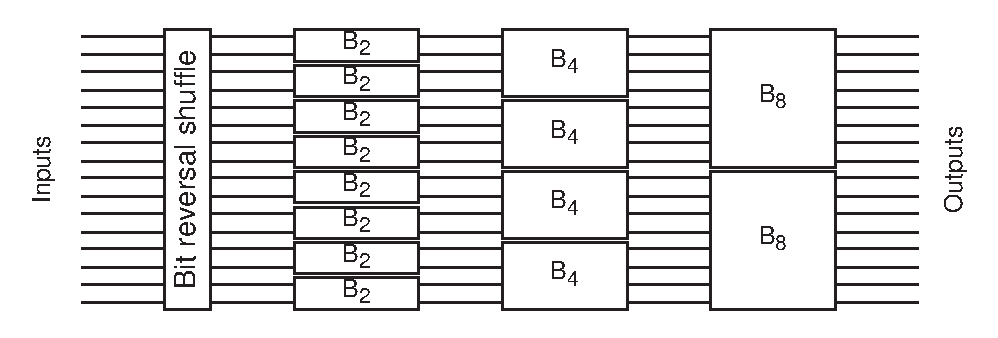
\includegraphics[width=11cm]{fftcomp}
\end{center}
\caption{FFT computation\label{Poly:FFTComp:Fig}}
\end{figure}

\smallskip
Although the algorithm described by \eqnref{FFT:Factor:Eq} appears to
be recursive, it turns out to be simpler if the column permutations
for all of the factors are performed at once.  The result is a single
reordering of the columns based on a very curious pattern.  Consider
what happens when
\eqnref{FFT:Factor:Eq} is applied twice to an $8\times8$ matrix.
Dealing only with the columns, we have
\[
A\Pi_8 = (A_0 \mid A_2 \mid A_4 \mid A_6 \mid A_1 \mid A_3 \mid A_5 \mid A_7).
\]
To apply \eqnref{FFT:Factor:Eq} to the copies of $\mathbf{F}_4$, we must
apply $\Pi_4$ to the first four columns and, separately, to the second
four columns, \ie,
\[
\begin{aligned}
(A_0 \mid A_2 \mid A_4 \mid A_6) \Pi_4 & = (A_0 \mid A_4 \mid A_2 \mid A_6),\\
(A_1 \mid A_3 \mid A_5 \mid A_7) \Pi_4 & = (A_1 \mid A_5 \mid A_3 \mid A_7),
\end{aligned}
\]
so
\[
A\Pi_8\Pi'_4 = 
  (A_0 \mid A_4 \mid A_2 \mid A_6 \mid A_1 \mid A_5 \mid A_3 \mid A_7).
\]
What has occurred is that we have sorted the columns, by the {\em bit
reversal} of their indexes.  This suggests a computational structure
as shown in \figref{Poly:FFTComp:Fig}.

\paragraph{Computational Framework}

Assume we have a vector of values $f^{(0)}_0, \ldots, f^{(0)}_{n-1}$
for which we want to compute the Fourier transform.  (We will use the
superscripts to indicate to which stage of the computation the value
corresponds.)  The first step is to reorder the $f_i$ by the bit
reversal of their indices, \ie, $f^{(1)}_i = f^{(0)}_{\mbox{rev}(i)}$,
where $\mbox{rev}(i)$ is the bit reversal of $i$.

The $f^{(1)}_i$ are now combined using a sequence of ``butterflies'' of
different sizes.  Each box in \figref{Poly:FFTComp:Fig} corresponds to
multiplication by the matrix
\[
B_r = \left(\begin{array}{cc} I_r & \Omega_r \\I_r & - \Omega_r
\end{array}\right),
\]
which we call a \keyi{butterfly}.  These matrices have precisely
two non-zero elements on each row.  Thus, when multiplying by $B_r$ we
have
\[
f^{(k+1)}_i \leftarrow f^{(k)}_i + \zeta f^{(k)}_{i+r}
\]
where $\zeta$ is an $n$-th root of unity.  It is convenient to
couple the computation of $f^{(k+1)}_i$ with that of
$f^{(k+1)}_{i+r}$:
\[
f^{(k+1)}_{i+r} \leftarrow f^{(k)}_i - \zeta f^{(k)}_{i+r}.
\]
We denote the pair of these computations by {\tt FFT2}:
\[
\mbox{\tt FFT2}[i, j, \zeta] \approx
\left\{
\left(\begin{array}{c} f^{(k+1)}_i \\ f^{(k+1)}_j \end{array}\right)
\leftarrow
\left(\begin{array}{cc} 1 & \zeta \\ 1 & -\zeta \end{array}\right)
\left(\begin{array}{c} f^{(k)}_i \\ f^{(k)}_j \end{array}\right)
\right\},
\]
where $\zeta$ is a root of unity.

The simplest computation is the 2 input butterfly, which consists of
just $\mbox{\tt FFT2}[2k, 2k+1, 1]$.  The four input butterfly
consists of two primitive computations:
\[
\mbox{\tt FFT2}[4k, 4k+2, \zeta_4^0], \mbox{\tt FFT2}[4k+1, 4k+3, \zeta_4^1],
\]
while the eight input butterfly consists of 
\[
\begin{array}{cc}
\mbox{\tt FFT2}[8k, 8k+4, \zeta_8^0],& 
  \quad \mbox{\tt FFT2}[8k+1, 8k+5, \zeta_8^1], \\
\mbox{\tt FFT2}[8k+2, 8k+6, \zeta_8^2],&
  \quad \mbox{\tt FFT2}[8k+3, 8k+7, \zeta_8^3].
\end{array}
\]

An implementation of the {\sc fft} consists of two parts: (1) a chunk of
code that shuffles the entries of $a_j$ to produce $a_j'$, and (2)
code that implements the sequence of butterflies.  In this discussion
we only discuss the second section.

The following routine replaces $f$ by its Fourier transform.  It
assumes that the length of $f$ is a power of $2$.
\begindsacode
FFT ($f$[n]) := $\{$ \\
\> FFT\=2 (i, j, $\zeta$) := $\{$ \\
\>\> $\left(\!\!\!\begin{array}{c}f\mbox{[i]}\\f\mbox{[j]}\end{array}\!\!\!\right)
  \leftarrow \left(\!\!\!\begin{array}{cc}1 & \zeta\\ 1 & -\zeta\end{array}\!\!\!\right)
  \left(\!\!\!\begin{array}{c}f\mbox{[i]}\\f\mbox{[j]}\end{array}\!\!\!\right)$;\\
\>\> $\}$; \\
\> FFT\=n (n, $k$) := $\{$ \\
\>\> unl\=ess $\mbox{n} = 2$ $\{$ \\
\>\>\> $\mbox{FFTn}(\mbox{n}/2, k)$;\\
\>\>\> $\mbox{FFTn}(\mbox{n}/2, k + \mbox{n}/2)$;\\
\>\>\> $\}$\\
\>\> loo\=p for $0 \le m < \mbox{n}/2$ do \{ \\
\>\>\> $\mbox{FFT2}(k+m, k+m+\mbox{n}/2, \zeta_{\mbox{m}})$; \\
\>\>\> $\}$ \\
\>\> $\}$ \\
\> $\mbox{FFTShuffle}(f)$; \\
\> $\mbox{FFTn}(\mbox{n}, 0)$; \\
\> $\}$
\enddsacode

\noindent
This routine uses two internal functions {\tt FFT2} and {\tt FFTn}.
{\tt FFT2} does 2 point butterfly.  The $n$ point butterfly is
implemented by the loop at the end of the {\tt FFTn}.  The first part
of {\tt FFTn} recursively computes the $n/2$ point butterflies.  

If we apply the Fourier transform and then the inverse Fourier
transform, as described by {\tt FFT}, to the same vector we will not
get the original vector, but $n$ times the original vector.  One
could deal with this problem either by adjusting the {\sc fft} routine
to remove a factor $\sqrt{n}$, or by removing a factor $n$ when
computing the inverse Fourier transform.

\medskip
One of the problems with the ``binary'' algorithm discussed in this
section is that the length of the vector transformed must be a power
of $2$.  In the years since the modern introduction of the {\sc fft}
algorithm \cite{Cooley1965-bp}, a vast number of extensions and variations
of the basic scheme discussed here have been developed.  Among these
variations are versions that permit the length of the algorithm to be
the product of small primes, \eg, $3^k$, and variations that merge the
argument shuffling we've used into the ``butterflies.''  Although all
of these methods asymptotically require $O(N \log N)$ operations, the
practical benefits they yield are very significant.

All of these {\sc fft} algorithms are valid over any field, $L$, that
contains $n$-th roots of unity.  If $L$ is either $\R$ or $\C$ then
$e^{2\pi i/n}$ can be used.  In this case, there are many good
libraries of {\sc fft} routines, including vectorized routines for
supercomputers \cite{Swarztrauber1984-zd,Bailey1988-ay,Bailey1988-rv}.  In the case
of $L = \R$ there are variants that encode two real numbers as a
single complex number thus decreasing the number stages in the {\sc fft} by
$1$.  It is also possible to combine two real valued vectors into a
single complex complex valued vector, also decreasing the number of
arithmetic operations by a factor 2. 

When $L$ is the rational integers, $\Z$, we can continue to use
$e^{2\pi i/n}$ as a primitive $n$-th root of unity\index{primitive root!of unity} if the round-off
errors introduced are carefully analyzed.  This is not the case when
$L$ is a finite field.  Assume that $L = \F_q$, so every element of
$L$ is a zero of $X^{q-1} - 1$, \ie, every element of $L$ is a root of
unity.  If $n$ divides $q-1$ then, by the discussion in
\sectref{FF:Multiplicative:Sec}, $L$ has $\phi(n)$ elements of order
$n$.  Each of these is a primitive $n$-th root of unity.   

If one needs an $n$-th root of unity that does not lie in $\F_q$,
then it can always be obtained by adjoining zeroes of irreducible
factors of $X^n-1$ to $\F_q$.  This however, can be quite expensive.
For instance, to interpolate a polynomial of degree $63$ over $\F_5$,
we need a $64$-th root of unity.  The smallest field of
characteristic $5$ with $64$-th roots of unity is $\F_{5^{16}}$.
Arithmetic in this field is at least $16 \log 16 = 64$ times more
expensive than arithmetic in $\F_5$.  So, the {\sc fft} approach here
is not likely to be of benefit.

\paragraph{FFT Based Interpolation}

The fast Fourier transform routine, {\tt FFT}, allows us to
interpolate the right type of black boxes exceedingly quickly.  Assume
that ${\cal B}_P$ represents a polynomial of degree $d$ over a field
$L$.  Let $n$ be $\lceil \log_2 d \rceil$ and assume that $\zeta \in
L$ is a primitive root of unity\index{primitive root!of unity} of
order $N = 2^n$.  Construct the set of values
\[
{\cal B}_P(1), {\cal B}_P(\zeta), {\cal B}_P(\zeta^2), {\cal
B}_P(\zeta^3), \ldots, {\cal B}_P(\zeta^{2^n-1}).
\]
The Fourier transform of this sequence will be the coefficients of
$P$.  The last $2^n - d$ of them should be zero.

The time required of this approach is $N = 2^{\lceil \log_2 d
\rceil}$ evaluations and $O(N \log N) = O(d \log d)$ operations for 
the {\sc fft}.

\medskip
It is informative to analyze the case of $L = \Z$ in a bit more
detail.  Assume that we are also given $B \ge |P|$, a bound on the
absolute value of the coefficients of $P$, in addition to $n$, a power
of two that bounds the degree of $P$.  Instead of performing the
interpolation over $\R$, we can instead choose a set of fields
$\F_{q_1}, \ldots, \F_{q_k}$, of characteristic $p_1, \ldots, p_k$
such that $n \mid (q_i -1)$ and such that $p_1 \cdots p_k \ge 2B + 1$.
Using $k \cdot n$ evaluations of ${\cal B}_P$ we can compute the image
of $P$ modulo the $p_i$.  The \key{Chinese remainder theorem} can now be
used to reconstruct $P$ over the integers.  The time required by such
an approach is
\[
O(k n \log n + n M_{\rm int}(\log B)^2)
\]
where $M_{\rm int}(\log B)$ is the time to multiply to integers of
$\log B$ bits.  Again this is asymptotically faster than the simpler,
Lagrangian and Newtonian interpolation algorithms discussed earlier,
but practically it is not of use except for univariate polynomials of
large degree.

\paragraph{Fast Polynomial Multiplication}

Let $F(X)$ and $G(X)$ be two polynomials over degree $m$ over a field
$L$,
\[
\begin{aligned}
  F(X) &= f_{m-1} X^{m-1} + f_{m-2} X^{m-2} + \cdots + f_0,\\
  G(X) &= g_{m-1} X^{m-1} + g_{m-2} X^{m-2} + \cdots + g_0.
\end{aligned}
\]
We want to compute $H(X) = F(X) G(X)$, were $\deg H = n = 2m$.  Using
classical multiplication we can do this using $O(n^2)$
multiplications.  We would like to do better using interpolation. 

We can easily construct a black box for $H$, ${\cal B}_H(x) = F(X)
G(x)$, when $x \in L$.  By choosing $n$ values of $x$ and using the
univariate interpolation techniques discussed earlier, we can
reconstruct $H$.  The cost however is still $O(n^2)$ multiplications.
Each evaluation of ${\cal B}_H$ requires $O(n)$ multiplications, so it
takes $O(n^2)$ multiplications to compute all of the values.  The
Newtonian and Lagrangian interpolation schemes themselves require
$O(n^2)$ operations.

However, by using the fast Fourier transform we can do better.  The
interpolation cost immediately drops from $O(n^2)$ to $O(n \log n)$.
In addition, we can compute all of the values of $F(X)$ and $G(X)$
using a single fast Fourier transform for each.  Thus we can bring the
total asymptotic cost of polynomial multiplication down to $O(n \log
n)$.  This technique for multiplying polynomials is the most efficient
known thus far.  However, all of the practical problems alluded to in
the previous section apply here also.  These problems are exacerbated
when dealing with multivariate polynomials, which frequently occur.

On the other hand, for moderate to large degree univariate polynomials
with coefficients in $\R$, $\C$, or, perhaps, small elements of $\Z$,
the {\sc fft} method can be quite effective.  When $L = \R$ this is
especially true if one uses an {\sc fft} routine that determines the
transform of two real functions at once using a single complex
transform.

\index{fast Fourier transform|)}


\section{Abstract Interpolation} 
\label{Interp:Abstract:Sec}

In this section we introduce a bit more abstraction into our
discussion of interpolation.  This will allow us to deal with a
variety of different types of interpolation problems in a uniform
framework.

Let $R$ be a commutative ring with unit and let $\mathfrak{m}$ be an
ideal of $R$.  Recall that $R/\mathfrak{m}$ is set of residue classes of
$R$ modulo $\mathfrak{m}$.  Two elements of $R$ $x$ and $y$ are in the
same equivalence class in $R/\mathfrak{m}$ if $x - y$ is an element of
the ideal $\mathfrak{m}$.  There is a natural map that sends elements of
$R$ to the equivalence classes in which they lie in $R/\mathfrak{m}$.
This map induces a ring structure on $R/\mathfrak{m}$.  If $\mathfrak{m}$ is
a \key{prime ideal} then $R/\mathfrak{m}$ is an \key{integral domain}.
If $\mathfrak{m}$ is a \key{maximal ideal} then $R/\mathfrak{m}$ is a field.

For many rings $R$ and ideals $\mathfrak{m}$ there is a canonical
representative for each class in $R/\mathfrak{m}$.  In such cases, we use
the canonical representative and the equivalence class
interchangeably.

Two common examples are $R = \Z$ and $R = L[X]$, where $L$ is a field.
The ideals of $\Z$ are principal, \ie, all ideals are generated by a
single element, $\mathfrak{m} = (m)$.  The canonical representatives of
the equivalence classes of the quotient ring $\Z/(m)$ are the integers
$\{0, 1, \ldots, m-1\}$ (using the \key{one sided presentation} of
\chapref{Finite:Fields:Chap}).  The prime ideals of $\Z$ are also
maximal.  If $m$ is prime them $\Z/(m)$ is a field.  If on the
other hand, $m$ is divisible by $p > 1$, then $p$ will be a zero
divisor and $Z/(m)$ cannot be an integral domain.

The ideals of $L[X]$ are also principal, but are generated by the
polynomials in $L[X]$.  Let $\mathfrak{m} = (m(X))$ be an ideal in
$L[X]$.  Since $L$ is a field, we can assume that $m(X)$ is monic.  As
with $\Z$, the canonical representatives in $L[X]/\mathfrak{m}$ are the
reduced residues modulo $m(X)$.  The case when $m(X)$ is linear occurs
frequently.  Let $a(X) \in L[X]$ be a polynomial, and assume $m(X) = X
- k$, where $k$ is an element of $L$.  The remainder of $a(X)$ when
divided by $X - k$ is $a(k)$.

For $a$ an element of a ring $R$, and $\mathfrak{m}$ an ideal of $R$, we
use the notation
\[
a(\mathfrak{m}) = a \mod\mathfrak{m}.
\]
Thus, if $\mathfrak{m} = (X - k)$ then $a(k) = a(\mathfrak{m}) = a((X -
k))$.  Note the extra set of parenthesis in the last form, which will
not be often used.  

\medskip
With this notation we can discuss interpolation in a manner that
strengthens the parallels between the Chinese remainder algorithm for
integers of \sectref{Integer:Chinese:Remainder:Sec} and that for
polynomials in \sectref{Interp:CRA:Sec}.  The following is the
standard version of the \key{Chinese remainder theorem}

\begin{proposition}[Chinese Remainder Theorem]
Let $\mathfrak{p}_1, \ldots, \mathfrak{p}_n$ be ideals in a ring $R$, such
that every pair is co-prime, \ie, $\mathfrak{p}_i + \mathfrak{p}_j = (1)$ if
$i\not=j$.  There is a one to one correspondence between $n$-tuples in
$R/\mathfrak{p}_1 \times \cdots \times R/\mathfrak{p}_n$ and $R/\mathfrak{p}_1
\cdots \mathfrak{p}_n$.
\end{proposition}

Let $\mathfrak{p}_1, \ldots, \mathfrak{p}_t$ be ideals in $R$ and $F$
be an element of $R$.  The interpolation problem is: Given
$F(\mathfrak{p}_1), \ldots, F(\mathfrak{p}_t)$ compute an element of
$R/\mathfrak{p}_1 \cdots \mathfrak{p}_t$ whose image in
$R/\mathfrak{p}_i$ is $F(\mathfrak{p}_i)$.  In the context of black
boxes, we have a black box ${\cal B}_F$ that accepts an ideal
$\mathfrak{q}$ and returns ${\cal B}_F(\mathfrak{q}) = F(\mathfrak{q})$.
Again our goal is reconstruct $F$.

Consider the simple case where there are only two ideals $\mathfrak{p}$
and $\mathfrak{q}$.  We are given $F(\mathfrak{p})$ and $F(\mathfrak{q})$ and
we want to compute $F(\mathfrak{pq})$.  Recall that when $R = \Z$ it was
necessary to require that the two moduli be relatively prime.  With
ideals, the same constraint is that $\mathfrak{p} + \mathfrak{q} = 1$.  That
is, there exist $a \in \mathfrak{p}$ and $b \in \mathfrak{q}$ such that
$a+b=1$.  Thus
\[
F(\mathfrak{pq}) = a F(\mathfrak{p}) + b F (\mathfrak{q}).
\]

In more generality, let $\mathfrak{p}_1, \ldots, \mathfrak{p}_t$ be pairwise
co-prime ideals in $R$ and define
\[
\mathfrak{P}_i = \mathfrak{p}_1 \cdots \mathfrak{p}_{i-1} \mathfrak{p}_{i+1}
\cdots \mathfrak{p}_t.
\]
The $\mathfrak{P}_i$ are defined so that 
\[
\mathfrak{P}_1 + \mathfrak{P}_2 + \cdots + \mathfrak{P}_t = (1)
\]
any smaller subset is divisible by some $\mathfrak{p}_j$.  Letting $p_i$
be elements of $\mathfrak{P}_i$ whose sum is $1$ gives,
\begin{equation}\label{CRA:Lagrange:Eq}
F(\mathfrak{p}_1 \cdots \mathfrak{p}_t) = 
 p_1 F(\mathfrak{p}_1) + p_2 F(\mathfrak{p}_2) + \cdots +
  p_t F(\mathfrak{p}_t).
\end{equation}

When $R = k[Z]$ this is precisely the \key{Lagrange interpolation
formula} discussed earlier.  Let $\mathfrak{p}_i = (Z - z_i)$, so
\[
\mathfrak{P}_i = \left((Z - z_0) \cdots (Z-z_{i-1})(Z-z_{i+1}) \cdots
(Z-z_t)\right)
\]
and
\[
p_i = \frac{(Z-z_0)\cdots(Z - z_{i-1})(Z - z_{i+1}) \cdots (Z-z_t)}{(z_i-z_0)\cdots(z_i - z_{i-1})(z_i - z_{i+1}) \cdots (z_i-z_t)}.
\]
The sum of the $p_i$ is a polynomial of degree $t$.  Its value at $Z =
z_0, z_1, \ldots, z_t$ is $1$ so it must be identically equal to $1$.

A Lagrangian interpolation formula can be developed for $R = \Z$ by
using \eqnref{CRA:Lagrange:Eq}.  Consider the simple case of two
ideals, $\mathfrak{p} = (p)$ and $\mathfrak{q} = (q)$.  Again, we are
looking for $a \in \mathfrak{p}$ and $b \in \mathfrak{q}$ such that $a+b =
1$ modulo $\mathfrak{pq}$.  Since  $a = xp$ and $b = yq$, we want to find
$x$ and $y$ such that 
\begin{equation} \label{Abs:Dio:Eq}
xp + yq = 1,
\end{equation}
where $x$ and $y$ are integers.  As we know this diophantine equation
has solutions if and only if $p$ and $q$ are relatively prime.  Let
$\bar{x}$ and $\bar{y}$ be solutions of \eqnref{Abs:Dio:Eq}.

If we have
\[
\begin{aligned}
F &= k_1 \pmod{p} \\
F &= k_2 \pmod{q}
\end{aligned}
\]
Then a Lagrangian interpolation formula for $F$ is
\[
F = \bar{x} \cdot  k_2 \cdot p + \bar{y} \cdot k_1 \cdot q \pmod{pq}.
\]

\section*{Notes}

\small

\notesectref{Vandermonde:Sec} \propref{Gen:Vandermonde:Prop} appears
in {\Polya} and {\Szego} \cite{Polya1978-hx}, Chapter 5, problem 48.
Additional partial results on generalized Vandermonde matrices are
contained in the work of {\MitchellO} \cite{Mitchell1881-cv}, and
{\EvansR} and {\Isaacs} \cite{Evans1976-dq}.

\notesectref{Poly:FFT:Sec}
The fast Fourier transform algorithm was first discussed in modern
terms by {\Cooley} and {\Tukey} \cite{Cooley1965-bp}, although the basic
ideas have been known by a variety of authors starting with {\Gauss}.
See \cite{Heideman1984-zr} for a historical survey.  More detailed
discussions of fast Fourier transform algorithms and their
applications are contained in 
\cite{Tolimieri1989-sz,Brigham1988-dw,Van_Loan1992-cb,Pollard1971-qy}.

{\CantorD} and {\Kaltofen} \cite{Cantor1991-rr} have generalized the {\sc fft}
polynomial multiplication technique to polynomials over arbitrary
algebras.  For univariate polynomials of degree $n$, their technique
requires $O(n \log n)$ multiplies and $O(n \log n \log \log n)$
additions.

Bonneau has studied the use of {\sc fft} to speed polynomial
multiplication
\cite{Bonneau1974-if}.

\normalsize

%$Id: interp.tex,v 1.1 1992/05/10 19:42:22 rz Exp rz $
\chapter{Multivariate Interpolation}
\label{Sparse:Interp:Chap}

Multivariate polynomial interpolation is a bit more complex than the
univariate interpolation techniques discussed in
\chapref{Interpolation:Chap}.  Because the number of possible terms in
a multivariate polynomial can be exponential in the number of
variables, techniques similar to those of \chapref{Zero:Testing:Chap}
must be used to avoid spending inordinate amounts of time computing
coefficients that are equal to zero.

\sectref{Interp:MDense:Sec} demonstrates how
the univariate interpolation schemes recursively give a
deterministic multivariate algorithm that takes time $O(d^v)$ to 
reconstruct a polynomial in $v$ variables of degree no more than $d$ in 
each from its values.  For dense polynomials, where the number of 
non-zero terms is $O(d^n)$, this is an efficient algorithm.  
\sectref{Interp:PSparse:Sec} gives a probabilistic interpolation algorithm that
takes $O(T^3)$ time to compute such a polynomial with $T$ non-zero terms 
from its values.  For practical 
implementations this appears to be the most efficient interpolation
algorithm for sparse polynomials.  In \sectref{Interp:ZSparse:Sec} we
demonstrate how this algorithm can be made deterministic.

\sectref{Interp:BenOr:Sec} presents a different interpolation scheme
that, unlike the algorithm of \sectref{Interp:ZSparse:Sec}, does not
require a bound on the degrees of the variables in $P$.
Theoretically, this algorithm has better performance than the
algorithm of \sectref{Interp:ZSparse:Sec}, but from a practical point
of view the probabilistic approach is preferable.


\section{Multivariate Dense Interpolation}
\label{Interp:MDense:Sec}

As pointed out in \chapref{Interpolation:Chap}, a polynomial in one variable
of degree $d$ can be determined from its values at $d+1$ points using
$O(d^2)$ arithmetic operations.  This result can be extended to
multivariate problems recursively.

Assume we are given a black box ${\cal B}_P$ for the polynomial
$P(X_1, \ldots, X_n)$ with a degree bound, $\deg_{X_i} P = d$.  
We can assume that $P$ has the form
\[
P(X_1, \ldots, X_n) = P_0(X_2, \ldots, X_n) X_1^d + 
\cdots + P_d(X_2, \ldots, X_n).
\]
Using the univariate interpolation schemes of the previous chapter
we can create black boxes ${\cal B}_{P_0}, \ldots, {\cal B}_{P_d}$, for
the $n-1$-variate coefficients of $P$ as follows:

To find the value of ${\cal B}_{P_i}(x_{20}, \ldots, x_{n0})$, choose
a sequence of $d+1$ different evaluations, points where the first
component is chosen at random and the last $n-1$ components are
$x_{20}, \ldots, x_{n0}$.  Applying the interpolation algorithms of
the last chapter, we can compute $P(X_1, x_{20}, \ldots, x_{n0})$:
\[
\left.
\begin{array}{c}
{\cal B}_P(x_{10}, x_{20}, \ldots, x_{n0}) \\ \vdots \\
{\cal B}_P(x_{1,d+1}, x_{20}, \ldots, x_{n0})
\end{array} \right\} \longrightarrow P(X_1, x_{20}, \ldots, x_{n0}).
\]
The coefficients of this polynomial are
\[
\begin{aligned}
P(X_1, x_{20}, \ldots, x_{n0}) 
   & = P_0(x_{20}, \ldots, x_{n0}) X_1^d + \cdots + P_d(x_{20}, \ldots, x_{n0}), \\
   & = {\cal B}_{P_0}(x_{20}, \ldots, x_{n0}) X_1^d + \cdots 
     + {\cal B}_{P_d}(x_{20}, \ldots, x_{n0}).
\end{aligned}
\]
So at the cost of $d+1$ evaluations, we can determine one value of
each of the $d+1$ black boxes, ${\cal B}_{P_0}, \ldots, {\cal B}_{P_d}$. 

This process is then repeated, but with a different value for the $X_2$
coordinate,
\[
\left.
\begin{array}{c}
{\cal B}_P(x_{10}, x_{21}, x_{30}, \ldots, x_{n0}) \\ \vdots \\
{\cal B}_P(x_{1,d+1}, x_{21}, x_{30}, \ldots, x_{n0})
\end{array} \right\} \longrightarrow P(X_1, x_{21}, x_{30}, \ldots, x_{n0}),
\]
which gives another value for each of the ${\cal B}_{P_i}$.  When
repeated $d+1$ times, $P(X_1, X_2, x_{30}, \ldots, x_{n0})$ can be
reconstructed as shown in \figref{SI:DenseAlg:Fig}

\begin{figure}
\small
\[
\hspace*{-14pt}\left.
\begin{array}{c}
\left.
\begin{array}{c}
{\cal B}_P(x_{10}, x_{20}, \ldots, x_{n0}) \\ \vdots \\
{\cal B}_P(x_{1,d+1}, x_{20}, \ldots, x_{n0})
\end{array} \right\} \rightarrow P(X_1, x_{20}, \ldots, x_{n0})\\
\vdots \\
\left.
\begin{array}{c}
{\cal B}_P(x_{10}, x_{2d}, \ldots, x_{n0}) \\ \vdots \\
{\cal B}_P(x_{1,d+1}, x_{2d}, \ldots, x_{n0})
\end{array} \right\} \rightarrow P(X_1, x_{2d}, \ldots, x_{n0})
\end{array} \right\}
\rightarrow P(X_1, X_2, x_{30}, \ldots, x_{n0})
\]
\normalsize
\caption{Dense Interpolation Scheme\label{SI:DenseAlg:Fig}}
\end{figure}

This recursive process can now be repeated with the $(d+1)^2$
coefficients $P(X_1, X_2, x_{30}, \ldots, x_{n0})$.  Each set of
coefficient values can be computed with $(d+1)^2$ values.  More
generally, the $(d+1)^k$ coefficients of $P(X_1, \ldots, X_k,
x_{k+1,0}, \ldots, x_{n0})$ can be computed with $(d+1)^k$ evaluations
of ${\cal B}_P$.  And thus $P(X_1, \ldots, X_n)$ can be determined
with $(d+1)^k$ values.

To analyze the complexity of this algorithm, let $I(d)$ denote the
time complexity of interpolating $d+1$ values to produce a univariate
polynomial of degree $d$.  And let $N_k$ be the complexity of the
previous algorithm for $k$ variables.  We have
\[
\begin{aligned}
N_1 & = I(d), \\
N_2 & = (d + 1) N_1 + (d+1)I(d), \\
& \vdots \\
N_k & = (d+1) N_{k-1} + (d+1)^{k-1} I(d).
\end{aligned}
\]
It is easy to show by induction that the solution to this recurrence
is
\[
N_k = k(d+1)^{k-1} I(d).
\]
Using a classical interpolation algorithm, $I(d) = O(d^2)$, so this
algorithm requires $O(n d^{n+1})$ operations.  Using evaluation points
that satisfy the requirements of the \key{fast Fourier transform}
reduces this cost to $O(n d^n \log d)$.

\section{Probabilistic Sparse Interpolation}
\label{Interp:PSparse:Sec}

This section develops the sparse interpolation algorithm
\cite{Zippel1990-ab}, which uses probabilistic techniques to interpolate a 
polynomial in time dependent on the number of non-zero terms.  This 
algorithm is given no information about the number of non-zero terms in 
the polynomial being interpolated. Instead it develops an estimate of the 
number of terms as each new variable is introduced.  As a consequence its 
performance depends upon the actual number of non-zero terms in the 
polynomial rather than an {\em a priori} bound.  For most practical 
problems, this appears to be the best algorithm available and tends to be 
more useful than the deterministic algorithms presented in the following 
sections \cite{Manocha1991-iq}.

This section has three parts.  The first demonstrates the sparse 
interpolation algorithm via an example. The next part gives a formal 
specification of the algorithm, while the final part analyzes the 
algorithm's performance. 

\paragraph{Heuristic Presentation}

As before, we wish to determine the polynomial $P(\vec X) \in L[\vec
X]$ from a black box ${\cal B}_P$, where $L$ is a field with
sufficiently many distinct elements.  We assume that $D$ bounds the
degree of $X_i$ in $P$.  The sparse interpolation algorithm computes
$P$ one variable at a time.  That is, we initially compute $P(a_1,
a_2, \ldots, a_n)$, then $P(X_1, a_2, \ldots,a_n)$, then $P(X_1, X_2,
a_3, \ldots, a_n)$ and so on, until we have determined $P(\vec X)$.
The introduction of each new variable is called a {\em stage} of the
algorithm.\index{stage!of interpolation algorithm}  We use clues from the 
polynomial produced in the preceding stage to minimize the effort 
required to produce the next polynomial in the sequence. 

The formal description of the sparse interpolation algorithm is rather
involved and it is easy to get bogged down by all the subscripts and
variables involved.  Nonetheless, the basic ideas behind the sparse
interpolation algorithm are fundamentally quite simple, as the
following example illustrates.

Let ${\cal B}_P$ be a black box representing the polynomial
\[
P(X, Y, Z) = 
  X^5 Z^2 + X^5 Z + X Y^4 + X Y Z^5 + Y^5 Z.
\]
We are given a degree bound of $5$ for each variable, so there are
$(5+1)^3 = 216$ different coefficients that need to be determined.
Given no other information, any deterministic interpolation scheme
would require $216$ calls to ${\cal B}_P$.  

Using either \keyw{LagrangeInterp} or \keyw{NewtonInterp}, the values
\[
{\cal B}_P(x_0, y_0, z_0), {\cal B}_P(x_1, y_0, z_0), \ldots, 
{\cal B}_P(x_5, y_0, z_0).
\]
can be interpolated to produce the polynomial:
\[
P(X, y_0, z_0) = c_0 X^5 + c_1 X + c_2.
\]
Having introduced the first variable, we have completed the first
stage.

The purpose of the second stage is to determine $P(X, Y, z_0)$.  The
dense interpolation scheme repeats the process of the previous
paragraph, using $6$ different evaluation points, to produce $P(X,
y_1, z_0)$.  The sparse interpolation scheme recognizes that $P(X,y_1,
z_0)$ probably only has $3$ non-zero coefficients and most likely has
the form
\[
P(X, y_1, z_0) = c_3 X^5 + c_4 X + c_5.
\]
Since there are only three unknown coefficients in $P(X, y_1, z_0)$,
only $3$ different values of ${\cal B}_P$ are needed to determine
them.  The overall computation of $P(X, Y, z_0)$ is shown in 
\figref{SI:SparseAlg:Fig}
\begin{figure}
\small
\[
\hspace*{-1pt}\left.\begin{array}{c}
\left.\begin{array}{c}
{\cal B}_P(x_0, y_0, z_0) \\ \vdots \\ {\cal B}_P(x_5, y_0, z_0)
\end{array}\right\} \rightarrow c_0X^5 + c_1 X + c_2 \\
\left.\begin{array}{c}
{\cal B}_P(x_0, y_1, z_0) \\ {\cal B}_P(x_1, y_1, z_0) \\ 
{\cal B}_P(x_2, y_1, z_0)
\end{array}\right\} \rightarrow c_3X^5 + c_4 X + c_5 \\
\vdots \\
\left.\begin{array}{c}
{\cal B}_P(x_0, y_5, z_0) \\ {\cal B}_P(x_1, y_5, z_0) \\ 
{\cal B}_P(x_2, y_5, z_0)
\end{array}\right\} \rightarrow c_{15}X^5 + c_{16} X + c_{17} 
\end{array}\right\} \rightarrow d_0 X^5 + (d_1 Y^4 + d_2 Y) X + d_3 Y^5
\]
\normalsize
\caption{Sparse Interpolation Scheme\label{SI:SparseAlg:Fig}}
\end{figure}

After the $6$ different univariate polynomials, $P(X, y_i, z_0)$ are
computed, their coefficients are interpolated to produce $P(X, Y,
z_0)$.  Notice that only $6 + 5 \times 3 = 21$ evaluations are needed
so far, while the dense interpolation scheme requires $36$.

The third stage proceeds in the same fashion, but with even greater
savings.  We want to compute the six polynomials
\[
P(X, Y, z_i) = d_{4i} X^5 Z + d_{4i+1} X Y^4 + d_{4i+2} X Y + d_{4i+3} Y^5,
\]
for $i = 0, \ldots, 5$.  $P(X, Y, z_0)$ is known from the second
stage, and we assume that all of the $P(X, Y, z_i)$ have the same skeleton
as $P(X, Y, z_0)$.

Since there are only four unknowns in $P(X, Y, z_i)$, each set of the
$d_i$'s can be determined using only four values from ${\cal B}_P$ and
solving the resulting system of linear equations.  These equations can
be solved in $O(N^3)$ time using classical Gaussian elimination.
Notice that this approach places absolutely no restrictions on the
values used for the interpolation points.  This is quite useful in
certain problems where the user of the interpolation algorithm has its
own restrictions to place on the evaluation points \cite{Rubinfeld1994-lq}.

However, if the interpolation algorithm is free to choose the
evaluation points then the $O(N^3)$ Gaussian elimination cost can be
reduced to $O(N^2)$ by choosing the values for $X$ and $Y$ so that the
system of equations be a transposed Vandermonde
system.\index{Vandermonde system!transposed} Consider, for instance,
the computation of $P(X,Y,z_1)$.  For randomly chosen $x_{\alpha}$ and
$y_{\alpha}$ compute the four values
\[
\{P(1,1,z_1), P(x_{\alpha},y_{\alpha},z_1),
  P(x_{\alpha}^2,y_{\alpha}^2,z_1),
  P(x_{\alpha}^3,y_{\alpha}^3,z_1) \}.
\]
This gives the following Vandermonde system of equations for $d_4$,
$d_5$, $d_6$ and $d_7$:
\[
\begin{aligned}
d_4 (x_{\alpha}^5)^0 + d_5 (x_{\alpha} y_{\alpha}^4)^0 +
  d_6 (x_{\alpha} y_{\alpha})^0 + d_7 (y_{\alpha}^5)^0
    & = {\cal B}_P(1,1,z_1), \\
d_4 (x_{\alpha}^5)^1 + d_5 (x_{\alpha} y_{\alpha}^4)^1 +
  d_6 (x_{\alpha} y_{\alpha})^1 + d_7 (y_{\alpha}^5)^1
    & = {\cal B}_P(x_{\alpha},y_{\alpha},z_1), \\
d_4 (x_{\alpha}^5)^2 + d_5 (x_{\alpha} y_{\alpha}^4)^2 +
  d_6 (x_{\alpha} y_{\alpha})^2 + d_7 (y_{\alpha}^5)^2
    & = {\cal B}_P(x_{\alpha}^2,y_{\alpha}^2,z_1), \\
d_4 (x_{\alpha}^5)^3 + d_5 (x_{\alpha} y_{\alpha}^4)^3 +
  d_6 (x_{\alpha} y_{\alpha})^3 + d_7 (y_{\alpha}^5)^3
    & = {\cal B}_P(x_{\alpha}^3,y_{\alpha}^3,z_1).
\end{aligned}
\]

Regardless of how the system of equations is created and solved, the 
computation of $P(X, Y, z_1)$ only requires $4$ values from ${\cal B}_P$,
rather than the $36$ values that a dense interpolation scheme 
requires.  $P(X, Y, z_2)$ through $P(X, Y, z_5)$ can be computed in the
same fashion.  Finally, the coefficients of these polynomials can be
interpolated using a univariate interpolation scheme to get $P(X, Y, Z)$.
The total number of evaluations performed is $6 + 5 \times 3 + 5
\times 4 = 41$, which is a substantial improvement over the $216$
evaluations required by the dense interpolation.

For interpolation problems with more variables, the same recursive
structure is repeated. 

\paragraph{Formal Presentation}

To fix our notation, assume we want to determine a sparse polynomial
$P(X_1, \ldots, X_n) \in L[\vec X]$ where $L$ is a field.  The degree
of each $X_i$ in $P$ is bounded by $d$ and there are no more than $T$
non-zero monomials in $P$, \ie,
\[
P(X_1, \ldots, X_n) = c_1 \vec{X}^{\vec{e}_1} + c_2 \vec{X}^{\vec{e}_2} +
\cdots + c_T \vec{X}^{\vec{e}_T}.
\]
We assume that we are given a black box ${\cal B}_P$ that returns 
$P(\vec{x})$ when given a vector of values $\vec{x}$.  The set of 
exponents of a polynomial is called its {\em skeleton},\index{skeleton!of 
a polynomial} \ie{}  \addsymbol{$\skel P$}{The skeleton of a polynomial} 
\[
\skel P = \{\vec{e}_1, \vec{e}_2, \ldots, \vec{e}_T \}.
\]
We denote the {\em projection of the skeleton}\index{skeleton!projection 
of} of $P$ to $X_1, \ldots,
X_k$, by $\skel_k P$ defined by 
\addsymbol{$\skel_k P$}{Projection of the skeleton of a polynomial to
the first $k$ variables}
\[
\skel_k P = \{\, (e_1, \ldots, e_k) \mid \exists \vec{e}\in \skel P \,.\,
   \vec{e} = (e_1, e_2, \ldots, e_k, \ldots)\,\}
\]
So $\skel_k P$ is the set of tuples consisting of the first $k$ components
of elements of $\skel P$.  Notice that for all  $x_{k+1}, \ldots,
x_n \in L$, 
\[
\skel P(X_1, \ldots, X_k, x_{k+1}, \ldots, x_n) 
\subseteq \skel_k P(X_1, \ldots, X_n).
\]
Equality almost always occurs, but it is not necessary.  For instance, let
$P(X_1, X_2)$ be the polynomial $X_1^2 + X_1 X_2 + X_1$.  Then 
\[
\begin{aligned}
\skel P(X_1, X_2) &= \{(2, 0), (1, 1) (1, 0)\}, \\
\skel_1 P(X_1, X_2) & = \{ (2), (1) \}, \\
\skel P(X_1, -1) & = \{ (2) \}.
\end{aligned}
\]

We say that $(x_1, \ldots, x_n)$ is a \keyi{precise evaluation point}
if 
\[
\skel P(X_1, \ldots, X_k, x_{k+1}, \ldots, x_n) 
= \skel_k P(X_1, \ldots, X_n).
\]
for all $k > 1$.  Otherwise, $(x_1, \ldots, x_n)$ is said to be an
\keyi{imprecise evaluation point}.  The results of 
\sectref{Interp:MDense:Sec} allow us to estimate the likelihood of 
imprecise evaluation points as follows.

\begin{proposition}\label{Imprecise:Prob:Prop}
Let $P(X_1, \ldots, X_n)$ be a polynomial over an integral domain $A$.
Assume $\deg_{X_i} P \le D$ and $\terms P = T$.  Let ${\cal S}$ be a
subset of $A$ of cardinality $B$.  Then the probability that $(x_1,
\ldots, x_n)$ is an imprecise evaluation point of $P$, $x_i \in S$ is
bounded above by
\[
\frac{n(n-1)D T}{2B}.
\]
\end{proposition}

\begin{proof}
For each $k$ we can write
\[
P(X_1, \ldots, X_n) = c_{1k}(X_{k+1}, \ldots, X_n) \vec{X}^{\vec{f}_{1k}}
+ \cdots +
c_{Tk}(X_{k+1}, \ldots, X_n) \vec{X}^{\vec{f}_{Tk}},
\]
where $f_{ik} \in \skel_k P$.  In order for $\vec{x}$ to be
an imprecise evaluation point, it must be the zero of one of the
$c_{ij}$.  We can add up the probabilities, variable by variable.  By
\longpropref{Zero:MPoly:Prop}, the probability that $\vec{x}$ will be
a zero of one of $c_{1k}, \ldots, c_{Tk}$ is no more than
\[
\frac{(n-k)dT}{B}.
\]
Summing these probabilities gives
\[
\frac{(n-1)dT}{B} + \frac{(n-2)dT}{B} + \cdots + \frac{dT}{B} =
\frac{n(n-1)dT}{2B}.
\]
\end{proof}

\medskip

For exposition purposes, we consider one stage of the interpolation.
Assume we have performed the first $k-1$ stages of the sparse interpolation
algorithm and are about to begin the $k$-th stage.  Throughout the
$k$-th stage, the values assigned to $X_{k+1}, \ldots, X_{n}$ do
not vary.  To simplify the notation, we omit them\footnote{In an
implementation this may be more than notational.  Eliminating the
variables that do not vary at this stage can save significant time
when computing the values of $P$.} and write
\[
P'(x_0, \ldots, x_k) = P(x_1, \ldots, x_k, x_{k+1,0}, \ldots, x_{n0}).
\]
From the $k-1$-th stage's computation we have
\[
P(X_1, \ldots, X_{k-1}, x_{k0}, \ldots, x_{n0}) = p_{10} {\vec X}^{\vec e_1} +
p_{20} {\vec X}^{\vec e_2} + \cdots + p_{T0} {\vec X}^{\vec e_T}.
\]
We now assume that $\skel_k P = \{\vec{e}_1, \ldots, \vec{e}_T\}$,
\ie, $(x_{10}, \ldots, x_{n0})$ is a precise evaluation point for $P$.
This is the probabilistic assumption that underlies the algorithm.

The computation of $P(X_1, \ldots, X_{k-1}, X_k)$ proceeds in two phases: 
First, we determine  
\[
P'(X_1, \ldots, X_{k-1}, x_{kj}) = 
p_{1j} {\vec X}^{\vec e_1} + p_{2j} {\vec X}^{\vec e_2} + \cdots + p_{Tj} {\vec
X}^{\vec e_T},
\]
for $j = 1, \ldots, n$ by the following technique:

For randomly chosen $x_{kj}$ perform the following: Pick a $k-1$-tuple
denoted by $(y_1, \ldots, y_{k-1}) = \vec y$, such that each of $m_i =
{\vec y}^{\vec e_i}$ are distinct. Since the ${\vec e_i}$ are known,
verifying that this is the case is easy.  This value allows
us to set up the following (non-singular) transposed
Vandermonde system\index{Vandermonde system!transposed} of linear equations
\begin{equation}
 \label{SPMod:Vandermonde:System:Eq}
\begin{aligned}
  P'(1, \ldots, 1, x_{k,1})
    &= p_{1j} + p_{2j} + \cdots + p_{Tj}, \\
  P'(y_1, \ldots, y_{k-1}, x_{kj})
    &= p_{1j} {\vec y}^{\vec e_1} + p_{2j} {\vec y}^{\vec e_2} + \cdots +
      p_{Tj} {\vec y}^{\vec e_T}, \\
  P'(y_1^2, \ldots, y_{k-1}^2, x_{kj})
    &= p_{1j} {\vec y}^{2\vec e_1} + p_{2j} {\vec y}^{2\vec e_2} + \cdots +
      p_{Tj} {\vec y}^{2 \vec e_T}, \\
    &\vdots\\
  P'(y_1^T, \ldots, y_{k-1}^T, x_{kj})
    &= p_{1j} {\vec y}^{T \vec e_1} + p_{2j} {\vec y}^{T \vec e_2} + \cdots
      + p_{Tj} {\vec y}^{T \vec e_T},
\end{aligned}
\end{equation}
which can be solved by the techniques of \sectref{Vandermonde:Sec} in
$O(T^2)$ time and $O(T)$ space.  The result is a polynomial
\[
P'(X_1, \ldots, X_{k-1}, x_{kj}),
\]
for each of $d$ values $x_{kj}$. 

Second, we independently interpolate the coefficients of each
monomial, using the dense interpolation algorithm.  The results of these
interpolations are combined to produce
\[
P'(X_1, \ldots, X_{k-1}, X_k) 
  = p_1(X_k) {\vec X}^{\vec e_1} + p_2(X_k) {\vec X}^{\vec e_2} 
     + \cdots + p_T(X_k) {\vec X}^{\vec e_T}.
\]
The dense interpolation yielded the univariate polynomials $p_i(X_k)$.
The $p_i(X)$ are in turn expanded to get:
\[
P(X_1, \ldots, X_{k}, x_{k+1,0},\ldots, x_{n0}) 
  = p_{10}' {\vec X}^{\vec e_1'} + p_{20}' {\vec X}^{\vec e_2'} 
    + \cdots + p_{T0}' {\vec X}^{\vec e_T'}.
\]
This is the value returned by the $k$-th stage.  We are ready to
begin lifting the next variable.

\medskip
The routine \keyw{SparseInterpStage} below implements this approach.
Its arguments are a $k-1$ variable polynomial that results from the
$k-1${\st} stage, a black box representing the polynomial $P(X_1,
\ldots, X_k)$, a bound on the degree of $X_k$ in $P$ and $k$.  Within
{\tt SparseInterpStage} we have used $L$ to denote the coefficient
domain of $P$.  \Marginpar{In the following fix the skeleton if
$P_{k-1}$ is zero.}

\begindsacode
SparseInterpStage ($P_{k-1}$, ${\cal B}_P$, $D$, $k$) := $\{$ \\
\> $S \leftarrow \skel P_{k-1}$; \\
\> $\ell \leftarrow \mbox{length}(S)$; \\
\> $\vec{y} \leftarrow \mbox{InitY}(L, k - 1)$; \\
\> $m[\cdot] \leftarrow \vec{y}^S$; \\
\> loo\=p for $1 \le i \le D$ do $\{$ \\
\>\> $x[i] \leftarrow \mbox{random}(L^{k-1})$; \\
\>\> $B \leftarrow \{{\cal B}_P(\vec{y}^0, x[i]), \ldots, 
  {\cal B}_P(\vec{y}^{\ell}, x[i])\}$; \\
\>\> $\mbox{\em Eq}[i, \cdot] \leftarrow \mbox{SolveVandermondeT}(m[\cdot], B[\cdot])$;\\
\>\> $\}$ \\
\> $P_k \leftarrow 0$; \\
\> loo\=p for $i \le j < \ell$ do $\{$\\
\>\> $P_k \leftarrow p_k + X^{S[j]} \cdot \mbox{NewtonInterp}(\mbox{\em Eq}[\cdot,
j], x[\cdot])$;\\
\>\> $\}$ \\
\> $\mbox{return}(P_k)$; \\
\> $\}$
\enddsacode

\noindent
The routine \keyw{InitY} provides the initial vector for $\vec{y}$.
{\tt InitY} needs to return values such that the $m_i =
\vec{y}^{\vec{e}_i}$ are distinct and thus the Vandermonde system will
be non-singular.\Marginpar{Explain what should be used in a practical
implementation, and what if $P_k{-1}=)$ above.}

If the coefficient domain is an integral domain of either
characteristic zero or sufficiently large finite characteristic then
this can easily be done.  When the characteristic of $L$ is zero
the image of $\Z$ in $L$ is isomorphic to
$\Z$.  \keyw{InitY} returns a vector consisting of the first $k-1$
rational primes, \ie, $2, 3, 5, 7, \ldots$.  By unique factorization
of elements of $\Z$ the $m_i$ must be distinct.  If the characteristic
of $L$ is finite, then the characteristic of $L$ must be larger than 
\begin{equation} \label{SI:FFBound:Eq}
(2 \cdot 3 \cdots p_n)^d \approx n^{c_1 nd}.
\end{equation}
to guarantee the $m_i$ are distinct.  In either case, the size of the
numbers involved in the interpolation are polynomial in the number
of variables and their degrees in the polynomial.

When the characteristic of $L$ is not larger than \eqnref{SI:FFBound:Eq} 
the problem of keeping the \key{Vandermonde matrix} from being singular is a 
bit more difficult.  Here we take the approach that \keyw{InitY} should 
just choose random values for components of $\vec{y}$ and estimate the 
likelihood that the resulting Vandermonde will be singular. 

The Vandermonde is a $T \times T$ matrix and thus we need at
least $T$ different values for the $m_i$.  Thus we must have, at
least, $q > T$.  If this is not the case then, as at the end of
\sectref{Zero:Deterministic:Sec}, we construct a finite extension
of $\F_q$ that does have enough elements and work in that extension.
Since we only need polynomially many distinct elements of the
finite field we do not need to find a large degree extension of
$\F_q$ and can again use the results of {\Adleman} and {\LenstraH}
\cite{Adelman1986-kb}. 

Since the $m_i = \vec{y}^{\vec{e}_i}$ are products of the $y_i$ it is
best not to allow any of the $y_i$ to be zero.  Let $g$ be a
\key{primitive root} of $\F^{\ast}_q$.  Then each $y_i$ is a power of
$g$, $y_i = g^{a_i}$ and 
\[
m_i = g^{\vec{a}\cdot \vec{e}_i}.
\]
The $m_i$ are distinct if and only if each is a different power of
$g$.  So for a fixed $\vec{a}$ we would like to know how likely
$\vec{a} \cdot \vec{e_i}$ is equal to $\vec{a} \cdot \vec{e_i}$ modulo
$q-1$.  We begin with an enumeration proposition that counts the
number of zeroes of $\vec{a} \cdot \vec{x} = 0 \mod{(q-1)}$.

\begin{proposition} \label{SPMod:Count:Solns:Prop}
Let $\vec a$ be a fixed $n$-tuple where each component is
an element of $\Z/(m)$, $c$ be the common GCD of the $a_i$ and
$m$.  Let $\vec x$ be an $n$-tuple whose components range over $\Z_m$.  Then
$\vec a \cdot \vec x$ takes on $m/c$ distinct values.  These values
divide the different $\vec x$ into $m/c$ classes each containing $c
m^{n-1}$ different $\vec x$.  In particular, $\vec{a} \cdot \vec{x} =
0 \mod{m}$ has $c m^{n-1}$ solutions.
\end{proposition}

\begin{proof}
First, we reduce to the case where $c = 1$.  Since $\vec a \cdot \vec x$ is
a multiple of $c$ for every $\vec x$, $\vec a \cdot \vec x$ can take on no more
than $m/c$ values, \ie, $0, c, 2c, \ldots$.  Let $\alpha c$ be one of these
values.  Each solution of 
\begin{equation}
{\vec a \cdot \vec x \over c} = \alpha \pmod{m/c} 
\label{Eq:c}
\end{equation}
gives rise to $c^n$ solutions of $\vec{a} \cdot \vec{x} = c \alpha
\mod{m}$.  Thus if we can show that \eqnref{Eq:c} has $(m/c)^{n-1}$
solutions, we are finished.  The rest of the proof is induction on the 
dimension of $\vec{a}$.

Consider the one dimensional case, $a x = b \mod{m}$.  Since $a$
and $m$ are relatively prime, there is exactly one value of $x$ that
satisfies the relation for every value of $b$, as required by the
proposition.

Now assume the proposition is true for all vectors $\vec a$ of
dimension less than $n$.  Let $\alpha$ be an arbitrary element of
$\Z/(m)$.  We want to show that $\vec a \cdot \vec x = \alpha
\mod{m}$ has $m^{n-1}$ zeroes.  Without loss of generality, we can
assume that $a_1$ is not zero.  If $a_1$ and $m$ are relatively prime
then for every choice of $a_2, \ldots, a_n$ there is a unique $a_1$
that satisfies the relation.  Thus there are $m^{n-1}$ zeroes of the
relation as desired.

Assume that $a_1$ and $m$ have a GCD of $g$.  The relation has no
zeroes if $g$ does not divide $a_2 x_2 + \cdots a_n x_n - \alpha$.
Thus we consider the number of zeroes of
\[
a_2 x_2 + \cdots a_n x_n = \alpha \pmod{g}.
\]
Notice that $a_2, \ldots, a_n$ cannot have a GCD dividing $g$.  Thus
this equation has $g^{n-2}$ zeroes modulo $g$.  Each is the image of
$(m/g)^{n-1}$ elements modulo $m$.  Thus there are $m^{n-1}/g$ choices
of $a_2, \ldots, a_n$.  Each one will give rise to $g$ choices for
$x_1$ giving the desired result.

Since $0$ is one of the possible values $\vec{a} \cdot \vec{x}$ the
last claim follows immediately.
\end{proof}

This result can now be used to answer the question raised above.

\begin{proposition} \label{Vandermonde:Vec:Indep:Prop}
Let $\vec{e}_1, \ldots, \vec{e}_T$ be $n$-tuples where each component is less
than $d$.  There exists no more than
\[
d \cdot T \cdot (T-1) \cdot (q-1)^{n-1} \over 2
\]
$n$-tuples $\vec{y}$ with components in $F_q$ such that for some $i$
and $j$, $\vec{y}^{\vec{e}_i}$ and $\vec{y}^{\vec{e}_j}$ are equal.
Equivalently, the probability that a randomly chosen $\vec{y}$ will
cause two of the $\vec{y}^{\vec{e}_i}$ to have the same value is
bounded above by
\[
{d \cdot T \cdot (T-1) \over 2 (q - 1)}.
\]  
\end{proposition}

\begin{proof}
Let $g$ be a generator of the multiplicative group $\F_q^{\ast}$.  Then
for each $n$-tuple $\vec X$ we can assign another $n$-tuple $\vec a$ such that
$X_i = g^{a_i}$, assuming no $X_i$ is zero.  The $a_i$ are elements of
$\Z/(q-1)$.  Two monomials $\vec X^{\vec e_i}$ and $\vec X^{\vec e_j}$ have the
same value when 
\[
\vec x^{\vec e_i} = g^{\vec a \cdot \vec e_i} = g^{\vec a \cdot \vec e_j}
\vec x^{\vec e_j}.
\]
That is, when $\vec a \cdot (\vec e_i - \vec e_j) = 0 \pmod{q-1}$.  By
\propref{SPMod:Count:Solns:Prop} there are $c (q -1)^{n-1}$ such zeroes,
where $c$ is the GCD of the elements of $\vec e_i - \vec e_j$ and $q-1$.
Since $c \le d$ there are at most $d (q -1)^{n-1}$ tuples $\vec x$ that
cause these two terms to take on the same value.

There are $T(T-1)/2$ distinct pairs of $\vec e_i$, so the maximum number of
$\vec x$ that cause a pair of $\vec x^{\vec e_i}$ to take on the same value is
\[
{d \cdot T \cdot (T-1) \cdot (q-1)^{n-1} \over 2}.
\]

Since there are only $(q-1)^{n}$ possible $\vec x$ (ignoring those
with a zero component), we have the proposition.
\end{proof}

Thus we need $q \gg dT^2$ to ensure that, with probability greater than 
$1/2$, the \key{Vandermonde system} is non-singular.  

\paragraph{Analysis}

To analyze the sparse interpolation algorithm, assume that we are given a
black box ${\cal B}_P$ representing a polynomial $P(X_1, \ldots, X_n)$
where the degree of each variable is bounded by $d$.  Furthermore, assume
that $P$ has no more than $t$ non-zero terms, but this parameter is not
provided to the algorithm.  

The probabilistic nature of the algorithm arises from two issues:
\begin{itemize}
\item[{\bf A}] The initial evaluation point must be precise.
\item[{\bf B}] The Vandermonde matrices generated must be non-singular. 
\end{itemize}

Let $\epsilon$ denote the likelihood of failure of the interpolation
algorithm.  For characteristic zero only the first probabilistic
assumption could fail, so by \propref{Imprecise:Prob:Prop}
\[
\epsilon < \frac{n(n-1)dT}{B}.
\]
For positive characteristic both probabilistic assumptions could fail.
Using Propositions~\ref{Imprecise:Prob:Prop} and
\ref{Vandermonde:Vec:Indep:Prop} we have
\[
\epsilon < \frac{n(n-1)dT}{q-1} + \frac{dT(T-1)}{2(q-1)} <
\frac{dT}{q-1}(2n^2 +T).
\]

Now consider the computational cost at each stage.  At the beginning
of stage $k$, we have a $P_{k-1}$, a polynomial in $k-1$ variables,
with no more than $t$ non-zero terms.  To introduce the $X_k$ we
compute $d$ additional polynomials, each of which has the same
skeleton as $P_{k-1}$.  In total, these $d$ polynomials require
$dt$ values from ${\cal B}_P$ and each can be computed using $O(t^2)$
time and $O(t)$ space.  The interpolation to produce $P_k$ consists of
at most $t$ individual dense interpolations, each of which 
interpolates $d+1$ points at a cost of $O(d^2)$ time and $O(d)$ space.
Thus the time required by the $k$-th stage is
\[
d \times O(t^2) + t \times O(d^2) = O(dt(d+t)).
\]
The complete interpolation of $P(X_1, \ldots, X_n)$ will require $n$ stages
and will thus require $O(ndt(d+t))$ time with a likelihood of failure
bounded by $\epsilon$.

Thus we have the following proposition.

\begin{proposition}
Let $P$ be a polynomial in $n$ variables, each of degree no more than $d$
and with $t$ ($> n$) non-zero terms.  Let $\epsilon>0$ be small
parameter.  Assume the coefficients of $P$ lie in
a field $L$ with at least 
\[
\frac{dT(2n^2 +T)}{\epsilon}
\]
elements.  If the components of the starting point for the sparse
interpolation algorithm is chosen from a subset of $L$ of at
least $B$ elements,
\[
B > \begin{cases}
\displaystyle\frac{n(n-1)dT}{\epsilon} & \text{if $L$ has characteristic zero,} \\
\displaystyle\frac{dT(2n^2 +T)}{\epsilon} & \text{if $L$ has positive characteristic,}
\end{cases}
\]
then the sparse interpolation algorithm will reconstruct $P$ in
$O(dt(d+t))$ arithmetic operations with probability of error less than
$\epsilon$.  
\end{proposition}

\section{Deterministic Sparse Interpolation with Degree Bounds}
\label{Interp:ZSparse:Sec}

The probabilistic algorithm given in \sectref{Interp:PSparse:Sec} can
be made deterministic by applying the same techniques used for 
deterministic zero testing in \sectref{Zero:Deterministic:Sec}. 
This adaptation requires degree bounds on $P$, but works for polynomials
over any field.  The techniques discussed in this section were
developed by {\Zippel} \cite{Zippel1990-ab} and, independently, by
{\Grigoriev}, {\Karpinski}, {\Singer} \cite{Grigorev1994-xo}.  The next
section gives a deterministic interpolation technique due to {\BenOr}
and {\Tiwari} that does not need degree bounds, only term bounds.
Unfortunately, this technique is only valid for polynomials over $\Z$.

In this section we will only describe how the two probabilistic
assumptions of the previous section can be removed---the detailed
construction of a deterministic interpolation and its analysis is
omitted.   

We retain the notation of the previous section.  If $L$ has
characteristic zero we need only eliminate the precise evaluation
assumption {\bf A}.  We need only find a single precise evaluation
point in order to get the correct skeleton.    That is, using the
notation of \propref{Imprecise:Prob:Prop}, for at least one starting
point none of the $c_{ij}$ vanish.  We can use
\longpropref{Interp:15:Prop} to generate an appropriate characterizing
sequence for the $c_{ij}$.

For characteristic zero, the problem is a bit more difficult, but
assumption {\bf A} can be satisfied using the technique of
\propref{Sparse:ZeroPoly:Prop} to reduce the problem to finding a
characterizing sequence for a set of no more than $nT$ univariate
polynomials each of degree less than $dn$.  To find a point such that
none of these polynomials vanish, we find the generator of an
extension of $\F_q$ of degree $n^2dT$ (using {\Adleman} and
{\LenstraH}'s result \cite{Adelman1986-kb}).  Precisely the same technique
can be used for condition {\bf B}.  When working in such a large
extension, the arithmetic operations will by quite expensive.  For
instance, multiplication will take $O(n^4 d^2 T^2)$ operations in
$\F_q$.  Nonetheless, this approach does show that sparse polynomial
interpolation over a field can be performed in time polynomial in $n$,
$d$ and $T$.

\section{Deterministic Sparse Interpolation without Degree Bounds}
\label{Interp:BenOr:Sec}

For simplicity assume that the polynomial being interpolated, $P(\vec
X)$ is an element of $\Z[\vec X]$ where $\Z$ is the rational integers.
For the case of polynomials over finite fields
\longpropref{Zero:Mon:Prop} and the following discussion apply, as was
in the case of the zero avoidance problem.  Unlike the probabilistic
algorithm given earlier, the only parameters we are given about
$P(\vec X)$ is the bound on the number of non-zero terms ($T$), and
the number of variables ($n$).

We assume that we are given a black box ${\cal B}_P$ for $P(\vec{X})$
and that $P$ has at most $T$ non-zero terms.  We write $P$ as
\[
P(\vec X) = c_1 {\vec X}^{\vec e_1} + c_2 {\vec X}^{\vec e_2} + \cdots +
c_T {\vec X}^{\vec e_T}.
\]
We will continue to let $d$ be the maximum degree to which any
$X_i$ appears in $P$, but it will only be used in the analysis.  It
will not be used in the algorithm itself.

If we choose a distinct prime for each $X_i$ then the quantities
${\vec X}^{\vec e_i} = m_i$ will all be distinct by unique
factorization.  These are the only evaluation points used in the
algorithm.  Denote the value of $P$ at the point ${\vec p}^j$ by $v_j
= P({\vec p}^j)$.  Each of the the $v_j$ gives us a constraint among
the $c_i$ and the $m_i$, {\em viz\/},
\begin{equation}
c_1 m_1^j + c_2 m_2^j + \cdots + c_T m_T^j = v_j.
\label{Eq:d}
\end{equation}

{\BenOr} and {\Tiwari}'s interpolation algorithm is significantly
subtler than the probabilistic one presented earlier.  It proceeds in
three basic steps:

\begin{itemize}

\item Compute the actual number of non-zero terms in $P$, $t$.

\item Determine the values of the $m_i$, and then the $\vec e_i$.

\item Find the values of the $c_i$.

\end{itemize}

The most difficult step is the second, where a quite clever technique
is used to find the $m_i$.

\def\Step#1{\smallskip\noindent{\bf Step #1:}}

\Step{1}
Notice that the rank of the system of equations \eqnref{Eq:d} is
exactly $t$, the number of non-zero monomials in $P$.  Thus $t$ can be
computed by taking the first $T$ equations, corresponding to $v_0,
v_1, \ldots, v_{T-1}$ and computing their rank.  This requires
$O(T^3)$ steps.

\Step{2}
Rather than determining the $m_i$ directly, we first find a polynomial
whose zeroes are the $m_i$.  It is easier to determine the
coefficients of this polynomial than the $m_i$ directly.  The roots of
this polynomial are then found using a $p$-adic version of Newton's
iteration.

Let 
\[
\begin{aligned}
  Q(Z) & = (Z - m_1) (Z - m_2) \cdots (Z - m_t)\\
    & = q_t Z^t + q_{t-1} Z^{t-1} + \cdots + q_0,
\end{aligned}
\]
where $q_t = 1$.  Note that $Q(m_i) = 0$.  Consider the sum 
\[
\sum_{1 \le j \le t} c_j Q(m_j) =
  \sum _{0 \le i < t} \left(c_1 m_1^i + \cdots + c_t m_t^i\right)\,q_i.
\]
The left hand side of the equation is clearly zero; while on the right the
coefficient of each of the $q_i$ is one of the $v_i$.  Thus
\[
0 = v_t + v_{t-1} q_{t-1} + v_{t-2} q_{t-2} + \cdots + v_0 q_0.
\]
We can get additional equations by summing
\[
\sum_{1 \le j \le t} c_j m_j^k Q(m_j) 
 = \sum_{0 \le i \le t} (c_1 m_1^{i+k} + \cdots + c_t m_t^{i+k}) q_i
\]
for $k = 0, 1, \ldots, t-1$.  This gives the Toeplitz system of linear
equations:\index{Toeplitz matrix}
\begin{equation} \label{Toeplitz:Eq}
\begin{aligned}
  v_0 q_0 + v_1 q_1 + v_2 q_2 + \cdots + v_{t-1} q_{t-1} &= - v_t\\
  v_1 q_0 + v_2 q_1 + v_3 q_2 +\cdots + v_{t} q_{t-1} &= - v_{t+1}\\
  \vdots\\
  v_{t-1}q_0 + v_{t} q_1 + v_{t+1} q_2 + \cdots + v_{2t-2} q_{t-1} &= -
    v_{2t-1}
\end{aligned}
\end{equation}

In general, it would be difficult to show that these equations are
non-singular, however, in this case we can factor the Toeplitz matrix
$\mathbf{V}$ as follows.  Let $\mathbf{V}$ denote the matrix
\[
\mathbf{V} = \begin{pmatrix}v_0 & v_1 & \cdots & v_{t-1} \\
v_1 & v_2 & \cdots & v_t \\
\vdots & & & \vdots\\
v_{t-1} & v_t & \cdots & v_{2t-2}\end{pmatrix}
\]
Then $\mathbf{V}$ is the product
\small
\[
\begin{aligned}
\begin{pmatrix}1 & 1 & \cdots & 1 \\
m_1 & m_2 & \cdots & m_t \\
\vdots & & & \vdots\\
m_1^{t-1} & m_2^{t-1} & \cdots & m_t^{t-1} \end{pmatrix}
\cdot
\begin{pmatrix}c_1 & 0 & \cdots & 0\\
0 & c_2 & \cdots & 0 \\
\vdots & & & \vdots \\
0 & 0 & \vdots & c_t\end{pmatrix}
\cdot
\begin{pmatrix}
1& m_1 & \cdots & m_1^{t-1}\\
1& m_2 & \cdots & m_2^{t-1}\\
\vdots& & & \vdots\\
1& m_t  & \cdots & m_t^{t-1}\end{pmatrix} \\
\qquad = \begin{pmatrix}v_0 & v_1 & \cdots & v_{t-1} \\
v_1 & v_2 & \cdots & v_t \\
\vdots & & & \vdots\\
v_{t-1} & v_t & \cdots & v_{2t-2}\end{pmatrix} 
\cdot
\begin{pmatrix}
c_1& c_2 m_1 & \cdots & c_t m_1^{t-1}\\
c_1 & c_2 m_2 & \cdots & c_t m_2^{t-1}\\
\vdots& & & \vdots\\
c_1& c_2 m_t  & \cdots & c_t m_t^{t-1}\end{pmatrix}
\end{aligned}
\]
\normalsize

So as long as the $m_i$ are distinct the \eqnref{Toeplitz:Eq} is
non-singular.  The system of equations \eqnref{Toeplitz:Eq} can be
solved either by Gaussian elimination in $O(t^3)$ time, or by using
the {\Berlekamp}-{\Massey} algorithm\index{Berlekamp-Massey algorithm}
\cite{Massey1969-oe,Blahut1983-jc} in time $O(nt^2)$. 

The $m_i$ can now be determined by finding the zeroes of $Q$.  Notice
that the roots are real, distinct and are integers, so they are quite
easy to find.  The following algorithm of {\Loos} \cite{Loos1983-nu} can be
used.  Choose a prime $\ell$ such that $Q(Z)$ is square-free when
considered as a polynomial over $\Z/(\ell)$.  Denote the $t$ roots of
this polynomial by $m_{i0}$.  Then each of the $t$ roots modulo $\ell$
can be lifted to a root modulo $\ell^{2^s}$ by \key{Newton's
iteration}:
\[
m_{i,k+1} - m_{ik} = - {Q(m_{ik}) \over Q'(m_{ik})} \pmod{\ell^{2^{k+1}}}.
\]
This iteration is central to Hensel method discussed in detail in
\sectref{Univariate:Newton:Sec}.

Once we know the $m_i$'s the $\vec e_i$ can be determined by factoring each of
the $m_i$.  This is not hard, because the only possible divisors of the $m_i$
are the first $n$ primes, which are explicitly known.

\Step{3}
Knowing the $m_i$ we can now determine the $c_i$ by solving the
\key{Vandermonde system} comprised of the first $t$ equations of type
\eqnref{Eq:d}.

The time required by this algorithm is dominated by either step 1,
$O(T^3)$, or step 2, $O(dn \log n t^3)$.

\medskip
This solution to the interpolation problem only works for polynomials
over a field of characteristic zero, or of huge characteristic as
discussed in \sectref{Interp:PSparse:Sec}.

\section*{Notes}

\small

\notesectref{Interp:MDense:Sec} This approach was first suggested by
{\BrownWS} \cite{Brown1971-jr}.

\notesectref{Interp:PSparse:Sec}  A different  approach to
interpolation over finite fields is discussed in \cite{Roth1991-tr}, where
interpolation of polynomials over $\F_2$ is discussed.

\notesectref{Interp:BenOr:Sec}  {\Kaltofen} \cite{Kaltofen1990-gz} has shown
that one should use a modular version of the {\BenOr}-{\Tiwari}
algorithm for efficiency.\Marginpar{Also see \cite{Schonhage1988-za} and \cite{Mansour1995-ab}.}

\normalsize

%$Id: poly-gcd.tex,v 1.1 1992/05/10 19:41:36 rz Exp rz $
\chapter[Polynomial GCD's: Interpolation Algorithms]{Polynomial GCD's\\Interpolation Algorithms}
\label{Poly:GCD:Chap}

\index{greatest common divisor!of polynomials|(}

We now use the interpolation algorithms of
Chapters~\ref{Interpolation:Chap} and \ref{Sparse:Interp:Chap} to
compute the {\sc gcd} of two polynomials.  This is the first of the
modern algorithms that we discuss.  Although the principles
behind the sparse polynomial {\sc gcd} algorithm are quite simple, the
final algorithm is more complex than any discussed thus far.

For preciseness, assume that we wish to compute the {\sc gcd} of two
multivariate polynomials, $F(X_1, \ldots, X_v)$ and $G(X_1, \ldots,
X_v)$ whose coefficients lie in an integral domain $R$.  Unless
otherwise stated, $R$ is either $\Z$, $\Q$ or $\F_q$.  When $R$ has
positive characteristic, we assume that $R$ has plenty of elements for
the interpolation process. Further assume that the {\sc gcd} of $F$ and
$G$ is $H(X_1, \ldots, X_v)$.  The {\sc gcd} problem for several
polynomials can be reduced to the two polynomial problem by the
technique of \sectref{PRS:Content:Sec}.

Historically, the motivation for the techniques discussed in this
chapter was the empirical observation that the {\sc gcd} of two
polynomials is very often $1$.  This is the worst case for
the classical {\sc gcd} algorithms discussed in \chapref{PRS:Chap},
all of which effectively compute something at least as large as the
resultant of $F$ and $G$.  Some technique needed to be
developed whose intermediate structures were no larger than either the inputs
or the {\sc gcd}.  Thus arose the interpolation ideas.

A naive approach to this problem is to choose random values for
$\vec{x}_i \in R^v$ and compute 
\[
\gcd(F(\vec{x}_i), G(\vec{x}_i)) = h_i \in R.
\]
One could then try to interpolate the $h_i$ to get $H$.
Unfortunately, as stated this algorithm does not work well, since it
assumes that $h_i = H(\vec{x}_i)$, which is not always the case.  A
trivial example is $F = X+1$ and $G = X-1$.  For odd integer values of
$x$, $2$ divides $\gcd(x+1, x-1)$ even though the {\sc gcd} of $F$ and $G$
is $1$.  Nonetheless, a variant of this technique is effective for
many problems over $\Z$ that involve a small number of variables.
This variant is described in \sectref{PGCD:Heuristic:Sec}.

To use the modular interpolation approach successfully, one
does not perform the {\sc gcd}'s in $R$ but rather in $R[X_v]$.  That is,
values are chosen for $X_1, \ldots, X_{v-1}$ and we compute the {\sc gcd} of
$F(\vec{x}_i, X_v)$ and $G(\vec{x}_i, X_v)$ where $\vec{x}_i \in
R^{v-1}$.  This {\sc gcd} is a univariate polynomial.  So rather than have a
single interpolation problem for {\sc gcd}, we have several problems, one
for each of the coefficients of the univariate polynomials.  As we
shall see, the likelihood that
\[
\gcd(F(\vec{x}_i, X_v), G(\vec{x}_i, X_v)) = H(\vec{x}_i, X_v)
\]
is quite high.

With both of these algorithms, the basic approach is {\em
probabilistic\/}.  One uses a technique that produces a polynomial
that is likely to be the {\sc gcd} of the $F$ and $G$, but is not
guaranteed to be the {\sc gcd}.  The candidate can then be verified by
\key{trial division}.  If the candidate is not the {\sc gcd} then a
randomization of some sort is applied and a new candidate is produced.

For the algorithms discussed here, if the candidate divides both $F$
and $G$ then it is the {\sc gcd} of $F$ and $G$.  In practice, this
\keyi{test division} is quite cheap.  An essential part of proving the
validity of the algorithm is to show that the candidates produced
cannot be proper divisors of the {\sc gcd}.

\section{Heuristic GCD}
\label{PGCD:Heuristic:Sec}

The ``Heuristic {\sc gcd}'' algorithm (called ``\key{GCDHeu}'' for short) is
one of the simplest and easiest to implement of the modern algorithms.
Its speed derives from the fact that most computer algebra systems
have carefully coded and efficient large precision integer arithmetic
packages.  Unfortunately, it is difficult to prove that it is
efficient for polynomials involving a large number of variables and
its practical efficiency decreases correspondingly.

\index{radix interpolation|(}
We begin with a new type of interpolation scheme, called \keyi{radix
interpolation}.  Let 
\[
F(X) = f_0 X^m + f_1 X^{m-1} + \cdots + f_m
\]
be a polynomial and assume $f_i \in \Z$.  Recall from
\chapref{PBounds:Chap} that
\[
|F| = \| \langle f_0, \ldots, f_m \rangle \|_{\infty} 
  = \max \{ |f_0|, \ldots, |f_m| \}.
\]

With the Lagrange or Newton interpolation schemes the values of $F$ at
$m+1$ points are needed to compute the coefficients of $F$.  However,
if we know the value of $F$ at a sufficiently large point, $F$ can be 
reconstructed using only a single value.  Let $\xi \ge 2 |F| + 1$ be a
large integer.  Then
\[
\begin {aligned}
  F(\xi) & = f_0 \xi^m + f_1 \xi^{m-1} + \cdots + f_m, \\
      & = \xi (f_0 \xi^{m-1} + \cdots + f_{m-1}) + f_m.
\end{aligned}
\]
The quantity in parentheses is an integer, so the remainder when
$F(\xi)$ is divided by $\xi$ is either $f_m$ or $f_m + \xi$ if $f_m$
is negative.  Obviously, we should modify the remainder calculation so
that it always returns $f_m$.

We call this type of remainder calculation, a \keyi{balanced
remainder}.  (This is similar to the {\em balanced presentation} used
for elements in a finite field as discussed in
\chapref{Finite:Fields:Chap}.)  Define \keyw{BalRem} for rational
integers as 
\begindsacode
Bal\=Rem ($p$, $q$) := $\{$ \\
\> $r \leftarrow \mbox{remainder}(p, q)$; \\
\> if $r < q/2$ then $r$ else $r - q$ \\
\> $\}$ 
\enddsacode

The constant term of $F(X)$ is $f_m = \mbox{\tt BalRem}(F(\xi),
\xi)$.  The linear term of $F(X)$, $f_{m-1}$ can be computed as
\[
\mbox{\tt BalRem}\left( \frac{ F(\xi) - f_m}{\xi}, \xi\right).
\]
This process can be repeated for all the other coefficients of $F(X)$.
Thus all the coefficients of $F(X)$ can be computed from $F(\xi)$ if
$\xi \ge 2 |F| + 1$.  Furthermore, the number of arithmetic operations
required is linear in the degree of $F$.  On average, $F(\xi)$ requires
approximately $m \log |F|$ bits, so the bit complexity of this
interpolation process is quadratic in the size of $F(X)$.

The following routine implements this approach. 
\index{RadixInterp@\protect\texttt{RadixInterp}}

\begindsacode
Rad\=ixInterp ($h$, $\xi$) := $\{$ \\
\> $i \leftarrow 0$; \\
\> $H \leftarrow 0$; \\
\> loo\=p while $h \not= 0$ do \{ \\
\>\> $h_i \leftarrow \mbox{BalRem}(h, \xi)$; \\
\>\> $H \leftarrow X^i h_i + H$; \\
\>\> $h \leftarrow (H - h_i)/\xi$; \\
\>\> $\}$ \\
\> return($H$); \\
\> $\}$
\enddsacode
\index{radix interpolation|)}

\medskip
Let $F(X)$ and $G(X)$ be univariate polynomials over $\Z$, whose {\sc gcd}
is $H(X)$,
\[
\begin{aligned}
F(X) &= f_0 X^m + f_1 X^{m-1} + \cdots + f_m, \\
G(X) &= g_0 X^n + g_1 X^{n-1} + \cdots + g_n.
\end{aligned}
\]
GCDHeu generates {\sc gcd} candidates by computing the integer {\sc gcd} of
$F(\xi)$ and $G(\xi)$, which we denote by $h$, and then reconstructing
$H(X)$ from $h$ using the procedure discussed above.  We denote by
$H_{\xi}(X)$ the candidate polynomial produced by this process, \ie,
\[
H_{\xi}(X) = \mbox{\tt RadixInterp}(\gcd(F(\xi), G(\xi)), \xi).
\]

There are two reasons why $H_{\xi}(X)$ might not be $H(X)$.  First,
the {\sc gcd} of $F(\xi)$ and $G(\xi)$ might not be $H(\xi)$.  If this is
the case then \keyw{RadixInterp} cannot possibly reconstruct $H(X)$.
Second, even if $\gcd(F(\xi), G(\xi)) = H(\xi)$, $\xi$ must be larger
than the coefficients of $H(X)$.  That is, $\xi > 2|H|+1$.  Since $H$
divides both $F$ and $G$, we can use \longpropref{Factor:CBound:Prop}
to bound the height of $H$:
\[
|H| \le (d+1)^{1/2} 2^d \max\{ |F|, |G| \},
\]
where $d = \max \{m, n\}$.  Thus $\xi$ should be chosen to be an
integer such that
\[
\xi > (d+1)^{1/2} 2^{d+1} \max\{ |F|, |G| \}.
\]

The following proposition, gives a necessary and sufficient condition
for $H_{\xi}(X)$ to actually be the {\sc gcd} of $F(X)$ and $G(X)$.

\begin{proposition}
Let $F(X)$ and $G(X)$ be univariate polynomials over the integers, and
$H_{\xi}(X)$ defined as above.  If $H_{\xi}(X)$ divides both $F(X)$
and $G(X)$ then $H_{\xi}(X)$ is the greatest common divisor of $F(X)$
and $G(X)$.
\end{proposition}

\begin{proof}
Let $H(X)$ denote a {\sc gcd} of $F(X)$ and $G(X)$ and let $A(X)$ and
$B(X)$ denote their {\em cofactors},\index{cofactor} \ie,
\begin{equation} \label{PGCD:HeuGCD:Eqa}
F(X) = H(X) A(X) \quad \mbox{and} \quad G(X) = H(X) B(X).
\end{equation}
By assumption $H_{\xi}(X)$ divides both $F(X)$ and $G(X)$, it must
divide $H(X)$,
\begin{equation} \label{PGCD:HeuGCD:Eqb}
H(X) = H_{\xi}(X) L(X).
\end{equation}
If $H_{\xi}(X)$ is not a {\sc gcd} of $F(X)$ and $G(X)$, then $L(X)$ will
not be $\pm 1$.

Letting $X= \xi$ in \eqnref{PGCD:HeuGCD:Eqb} gives
\[
H(\xi) = H_{\xi}(\xi) L(\xi)
\]
Letting $X = \xi$ in \eqnref{PGCD:HeuGCD:Eqa} shows that $H(\xi)$ must
divide $H_{\xi}(\xi) = \gcd(F(\xi), G(\xi))$, so
\[
L(\xi) \times \frac{H_{\xi}(\xi)}{H(\xi)} = 1
\]
where each factor is an integer.  Thus $L(\xi) = \pm 1$.  Since $L(X)$
divides $H(X)$, it must also divide $F$ and $G$ and thus we have the
same height bound for $L(X)$ as for $H(X)$.   Using \keyw{RadixInterp}
we see that $L(X) = \pm 1$.
\end{proof}

\section{Univariate Polynomials over \texorpdfstring{$\Z$}{Z}}
\label{PGCD:Uni:Sec}

For simplicity we first consider the problem of computing the {\sc gcd} 
of two polynomials 
\[
\begin{aligned}
F(X) & = f_0 X^r + f_1 X^{r-1} + \cdots + f_r, \\
G(X) & = g_0 X^s + g_1 X^{s-1} + \cdots + g_s, 
\end{aligned}
\]
over the rational integers $\Z$,
where we denote the {\sc gcd} by 
\[
\gcd(F, G) = H(X) = h_0 X^t + h_1 X^{t-1} + \cdots + h_t.
\]  
The approach is to pick a sequence of prime numbers $p_i$ and compute the 
{\sc gcd} of the images of $F(X)$ and $G(X)$ over $\Z/(p_i)$.  These 
polynomials are then interpolated using the \key{Chinese remainder theorem} to 
get a polynomial over the integers, which we expect to be $H(X)$. 

Two issues immediatedly arise with this approach.  First, we need a
bound on the size of the coefficients of $H(X)$ in terms of the size
of the coefficients of $F(X)$ and $G(X)$.  This bound indicates how many 
images modulo $p_i$ are needed.\, and is provided by 
\longpropref{Factor:CBound:Prop}.  Since $H(X)$ 
divides both $F(X)$ and $G(X)$, we have
\[
|H| \le \min( 2^r\sqrt{r+1} |F|, 2^s\sqrt{s+1} |G|).
\]

Second, and more importantly, $\Z$ is not a field while $\Z/(p_i)$ is.
Using a polynomial remainder sequence over a field always produces a
monic polynomial, while the {\sc gcd} of $F$ and $G$ might not be
monic.  Assuming the degree of this {\sc gcd}, $H_{p_i}(X)$ is $t$, it
is always the image of the monic version of $H(X)$, \ie,
\[
H_{p_i}(X) = X^t + \frac{h_1}{h_0} X^{t-1} + \cdots + \frac{h_t}{h_0}
    \pmod{p_i}.
\]
Now, assume we have computed the {\sc gcd} of $F(X)$ and $G(X)$ modulo
several primes and interpolated the results to produce a (necessarily) monic
polynomial
\[
H_m(X) = X^t + \frac{h_1}{h_0} X^{t-1} + \cdots + \frac{h_t}{h_0} \pmod{m},
\]
where $m > (2 |H| + 1) \gcd(f_0, g_0)$.  If we knew $h_0$, we could
recover $H(X)$ by simply multiplying $H_m(X)$ by $h_0$ modulo $m$,
converting to a balanced representation and interpreting the
coefficients as rational integers.

Assume for the moment that $F(X)$ and $G(X)$ are primitive, so, $H(X)$
is also primitive.  Although we do not know $h_0$, we do know that
$f_0$, $g_0$ and $\gcd(f_0, g_0)$ are all multiples of $h_0$.
Multiplying $H_m(X)$ by $\gcd(f_0, g_0) = a h_0$, and interpreting the
coefficients as rational integers gives $aH(X)$.  We can now determine
$H(X)$ by computing the principal part of $aH(X)$.

This process is called {\em imposing a leading
coefficient}\index{leading coefficient!imposing a} on a factor.  It is
a very useful technique that is often used for other problems.

The remaining detail is to establish a bound on the height of $aH(X)$.
Since $a$ divides $f_0$ and $g_0$, we have 
\[
|a H| \le |\gcd(f_0, g_0)| \cdot |H| 
  \le |\gcd(f_0, g_0)| \cdot \min( 2^r\sqrt{r+1} |F|, 2^s\sqrt{s+1}
|G|).
\]
Using this bound and the technique given above we get the following
algorithm for computing the {\sc gcd} of two univariate polynomials over the
rational integers.\Marginpar{Need to add a test divide at the end of
the following routine.}

\begindsacode
UnivariateGCD ($F$, $G$) : = \{ \\
\> $c \leftarrow \gcd(\cont F, \cont G)$; \\
\> $F \leftarrow \prim F$; $G \leftarrow \prim G$; \\
\> $h \leftarrow \gcd(\lc F, \lc G)$; \\
\> $\ell \leftarrow \lcm(\lc F, \lc G)$; \\
\> $r \leftarrow \deg F$; $s \leftarrow \deg G$; \\
\> $B \leftarrow 2 |h| \cdot \min( 2^r\sqrt{r+1} |F|, 2^s\sqrt{s+1}
|G|) + 1$; \\
\> $H \leftarrow 0$; \\
\> $m \leftarrow 1$; \\
\> loo\=p $\mbox{\rm choose a random prime $p$ such that $\ell \not=0 \mod{p}$}$ do \{ \\
\>\> $\hat{H} \leftarrow \gcd(F(X), G(X)) \mod{p}$; \\
\>\> if $\deg \hat{H} > \deg H$ $\mbox{\rm throw out $\hat{H}$ and $p$
and try again}$; \\
\>\> if \=$\deg \hat{H} < \deg H$ then \{ \\
\>\>\> $H \leftarrow \hat{H}$; \\
\>\>\> $m \leftarrow p$; \\
\>\>\> \} \\
\>\> if $\deg \hat{H} = \deg H$ then \{ \\
\>\>\> $H \leftarrow \mbox{\rm Apply the Chinese remainder algorithm to $H$
and $\hat{H}$}$; \\
\>\>\> $m \leftarrow m \cdot p$; \\
\>\>\> if $m > B$ then exit; \\
\>\>\> \} \\
\>\>\} \\
\> $H \leftarrow \mbox{\rm Balance $h \cdot H$ and convert to a polynomial
over $\Z$}$; \\
\> return($c \cdot \prim(H)$); \\
\> \}
\enddsacode

The first few steps of {\tt UnivariateGCD} compute the {\sc gcd} of the
content of $F$ and $G$, and replace $F$ and $G$ by  their primitive
parts.  Note that we want $F$ and $G$ to be primitive even if $c= 1$.
Otherwise the leading coefficient fix up technique does not work.  We
then compute $h$, a multiple of the leading coefficient of $\gcd(F,
G)$, and $B$, a bound on the size of the coefficients in $\gcd(F, G)$.

The core of the algorithm is the loop.  Throughout the loop $H =
\gcd(F, G) \mod{m}$.  Random primes $p$ are chosen for which the
degrees of $F$ and $G$ do not change.  $\hat{H}$ is then set to
$\gcd(F, G) \mod{p}$.  If $\deg \hat{H} \not= \deg H$ then the one
with the larger degree includes extraneous divisors and is discarded.

\paragraph{Analysis}

The crucial issue in analyzing \keyw{UnivariateGCD} is determining how
many {\sc gcd}'s modulo $p$ are computed.  Two issues arise here.
First, some of the {\sc gcd}'s will be useless because they produce
polynomials whose degree is too large.  Second, how large should the
primes $p$ be chosen so as to minimize the total amount of computation
in the {\sc gcd}'s modulo $p$.

We consider the second question first, since it is the easiest.
Assume that all of the {\sc gcd}'s yield polynomials of degree $t$ and
that the primes chosen, $p$, are all around $N$.  Then the number of
{\sc gcd}'s needed will be 
\[
k = \left\lceil \frac{\log B}{\log N} \right\rceil.
\]
Each {\sc gcd} will cost $C_{\gcd(F,G)} \cdot C_{M}(\log N)$ bit
operations, where $C_{\gcd(F,G)}$ is the number of arithmetic
operations required to compute the {\sc gcd} of $F$ and $G$, and
$C_{M}(M)$ is the number of bit operations required to multiply two
integers of $M$ bits.  

Increasing the size of the primes decreases the number of {\sc gcd}'s,
but increases the number of bit operations required to compute them.
Since $C_{M}$ grows faster than linearly, increasing the size of $N$
does not improve the total cost.  Decreasing $N$ below the word size
of the computer (the intrinsic parallelism of the machine) also does
not improve the total cost.

\smallskip
Now consider what must happen for $H_p(X)$ to have degree greater than
$t$.  Let $F(X) = \bar{F}(X) \cdot H(X)$ and $G(X) = \bar{G}(X) \cdot
H(X)$, where the cofactors $\bar{F}$ and $\bar{G}$ are relatively prime
over $\Z$.  Denote the degree of $\bar{F}$ by $\bar{r}$ and the degree
of $\bar{G}$ by $\bar{s}$.  If the prime $p$ leads to a false {\sc gcd},
then $\bar{F}$ and $\bar{G}$ are not relatively prime modulo $p$.
Since $\bar{F}$ and $\bar{G}$ have a common factor if and only if
their resultant vanishes, $p$ must divide $M = \res (\bar{F},
\bar{G})$.  \longpropref{Resultant:Bound:Prop} gives a bound on the
size of $M$: 
\[
|M| \le (\bar{r} + \bar{s})!\, |\bar{F}|^{\bar{r}} |\bar{G}|^{\bar{s}}.
\]
Using \longpropref{Factor:CBound:Prop}, we have
\[
\begin{aligned}
|\bar{F}| & \le 2^r \sqrt{r+1} |F|, \\
|\bar{G}| & \le 2^s \sqrt{s+1} |G|.
\end{aligned}
\]
Bounding $\bar{r} \le r$ and $\bar{s} \le s$ we have:
\[
|M| \le (r+s)! 2^{r^2+s^2} (r+1)^{r/2} (s+1)^{s/2} |F| \, |G|.
\]
Thus there are only a finite number of primes $p$ such that $H_p(X)$
does not have degree $t$.

\paragraph{Refinements}

Let the cofactors\index{cofactor} of $F$ and $G$ be $A$ and $B$ respectively, and
denote their images modulo $p$ by $\hat{A}$ and $\hat{B}$.  Given $F$
and $G$, and any one of $A$, $B$ or $H$ the other two can be computed
by two exact polynomial divisions.  So it does not really matter which
of $A$, $B$ or $H$ is computed in the {\sc gcd} algorithm.

The cost of a {\sc gcd} algorithm is dominated by the interpolations
used to combine the different $\hat{H}$ to produce $H$, and this cost
is a function of the size of $H$.  If one cofactor, say $A$, is much
smaller than the {\sc gcd} then it is more efficient to compute
$\hat{A}$ from $\hat{H}$ and use the Chinese remainder
algorithm\index{Chinese remainder theorem} to produce
$A$.\Marginpar{Expand on this}

The benefit of this approach for univariate polynomials is small, but
it is well worth the effort for multivariate {\sc gcd}'s.

\section{Multivariate Polynomials}
\label{PGCD:Multi:Sec}

The multivariate {\sc gcd} algorithm can be viewed as many copies of
the sparse interpolation scheme of \sectref{Interp:PSparse:Sec}.
Assume we wish to compute $H$, the {\sc gcd} of $F$ and $G$, where
\[
\begin{aligned}
F(X_1, \ldots, X_v) & = f_0(X_1, \ldots, X_{v-1}) X_v^m + \cdots + f_m(X_1,
\ldots, X_{v-1}), \\
G(X_1, \ldots, X_v) & = g_0(X_1, \ldots, X_{v-1}) X_v^n + \cdots + g_n(X_1,
\ldots, X_{v-1}), \\
H(X_1, \ldots, X_v) & = h_0(X_1, \ldots, X_{v-1}) X_v^r + \cdots + h_r(X_1,
\ldots, X_{v-1}).
\end{aligned}
\]
In essence we construct black boxes that represent the $h_i$:
\[
{\cal B}_{h_i}(y_1, \ldots, y_{v-1}) 
  = \coef(\gcd(F(y_1, \ldots, y_{v-1}, Z), G(y_1, \ldots, y_{v-1}, Z)), Z^i),
\]
and then use sparse interpolation methods to produce the $h_i(X_1,
\ldots, X_v)$ and thus $H$.  The actual algorithm, however, is
slightly complicated by (1) the desire to minimize the number of
univariate {\sc gcd} calculations, (2) the need to impose the leading
coefficient and (3) other performance considerations.

\begin{figure}
\begindsacode
SparseGCD1 ($\ell(X_1, \ldots, X_k)$, $F(X_1, \ldots, X_k; Z)$, $G(X_1, \ldots, X_k; Z)$) := \{\\
\>if $k= 0$ then return($\ell \times \gcd(F, G)$); \\
\>els\=e \{ \\
\>\> $d \leftarrow \min(\deg_{X_k} F, \,\,\deg_{X_k} G)$; \\
\>\> $x_k \leftarrow \mbox{random}(K)$; \\
\>\> $I \leftarrow \mbox{SparseGCD1}(F(X_1, \ldots, X_{k-1}, x_k; Z),
G(X_1, \ldots, X_{k-1}, x_k; Z))$; \\
\>\> $T_k \leftarrow \mbox{\rm Maximum number of terms in the coefficients of $I$}$; \\
\>\> for \=$1 \le i \le d$ do \{ \\
\>\>\> $y_i \leftarrow \mbox{random}(K)$; \\
\>\>\> $W \leftarrow \mbox{SparseGCD2}($\=$\skel I, \ell(X_1, \ldots, X_{k-1}, y_i),$ \\
\>\>\>\> $F(X_1, \ldots, X_{k-1}, y_i; Z), G(X_1, \ldots, X_{k-1}, y_i; Z), T_k)$;\\
\>\>\> for \=$0 \le j \le D$ do \{ \\
\>\>\>\> ${\cal H}_j \leftarrow {\cal H}_j \cup \{(y_i, \coef(W, Z^j))\}$; \\
\>\>\>\> \} \\
\>\>\> \} \\
\>\> for \=$0 \le j \le D$ do \{ \\
\>\>\> $\mbox{\rm Dense interpolate the coefficients of the monomials in
$X_1, \ldots, X_k$}$\\
\>\>\> $\mbox{\rm of the elements of ${\cal H}_j$ to get $h_j$.}$\\
\>\>\> \} \\
\>\> $H \leftarrow h_d Z^d + h_{d-1} Z^{d-1} + \cdots + h_0$; \\
\>\> $\mbox{\rm If $H$ does not divide both $F$ and $G$ start again
with a new evaluation point.}$\\
\>\> return($H$); \\
\>\> \} \\
\> \}
\enddsacode
\hrule
\begindsacode
SparseGCD2 ($S$, $\ell(X_1, \ldots, X_k)$, $F(X_1, \ldots, X_{k}; Z)$, $G(X_1, \ldots, X_{k}; Z)$, $T_k$) := \{\\
\>if $k=0$ then return($\ell \times \gcd(F, G)$); \\
\>els\=e \{ \\
\>\> $\mbox{\rm set $y_1, \ldots, y_k$ to random non-zero elements of $K$}$ \\
\>\> for \=$1 \le i \le T$ do \{ \\
\>\>\> $W \leftarrow \ell(y_1^i, \ldots, y_k^i) \times \gcd(F(y_1^i, \ldots, y_k^i; Z), G(y_1^i, \ldots, x_k^i; Z))$;\\
\>\>\> for \=$0 \le j \le D$ do \{ \\
\>\>\>\> ${\cal H}_j \leftarrow {\cal H}_j \cup \{(i, \coef(W, Z^j)) \}$;
\\
\>\>\>\> \} \\
\>\>\> \} \\
\>\>\> for \=$0 \le j \le D$ do \{ \\
\>\>\> $\mbox{\rm Use {\tt SolveVandermondeTD} to interpolate the elements of
${\cal H}_j$, in}$\\
\>\>\> $\mbox{\rm accordance with $\coef(S, Z^j)$, to get $h_j$}$\\
\>\>\> \} \\
\>\> return($h_d Z^d + h_{d-1} Z^{d-1} + \cdots + h_0$); \\
\>\> \} \\
\> \}
\enddsacode

\caption{Sparse Modular {\sc gcd} Algorithm \label{SparseGCD:Fig}}
\end{figure}

We single out one variable that will remain throughout the different
evaluations.  For simplicity, assume that the variable is $X_v$ and
throughout replace $X_v$ by $Z$.  We assume that $D$ bounds the degree
of each of $X_1, \ldots, X_{v-1}$ in $F$ and $G$.  The core of the
sparse {\sc gcd} algorithm is contained in the two routines in
\figref{SparseGCD:Fig}.

It is convenient to write
\[
\begin{aligned}
F^{(i)} &= F^{(i)}(X_1, \ldots, X_i; Z) = 
F(X_1, \ldots, X_i, x_{i+1}, \ldots, x_{v-1}, Z), \\
& = f^{(i)}_0(X_1, \ldots, X_i) Z^m + f^{(i)}_1(X_1, \ldots, X_i) Z^{m-1} 
 + \cdots f^{(i)}_m(X_1, \ldots, X_i),
\end{aligned}
\]
and similarly for $G^{(i)}$ and $H^{(i)}$.  The top level routine of
the algorithm, \keyw{SparseGCD1}, is initially invoked on $F^{(v-1)}$
and $G^{(v-1)}$ and recursively calls itself on $F^{(v-2)}$ and
$G^{(v-2)}$ and so on.  The {\sc gcd} is constructed from the bottom
up, producing $H^{(0)}$, then $H^{(1)}$ and so on.  We call the
construction of $H^{(k)}$ from $H^{(k-1)}$, where the variable $X_k$
is introduced into the {\sc gcd}, the $k$-th stage of the
computation.

Initially, we assume that $F$ and $G$ are monic.  In this case
the polynomials $\ell$, which represent leading coefficients, are
equal to $1$ and can be ignored.

In the zeroth stage, when $F$ and $G$ are univariate polynomials
in $Z$, a standard polynomial remainder sequence {\sc gcd} algorithm
can be used to compute
\[
H^{(0)} = \gcd(F^{(0)}, G^{(0)}) = 
\gcd(F(x_1, \ldots, x_{v-1}, Z), G(x_1, \ldots, x_{v-1}, Z)).
\]
All of the references to {\sc gcd} calculations in
\figref{SparseGCD:Fig} are of univariate {\sc gcd}'s that can also use
polynomial remainder sequence algorithms.

Assume we have computed $H^{(k)}$, the {\sc gcd} of $F^{(k)}$ and $G^{(k)}$.
Denote by $T_k$ the maximum number of non-zero monomials in the
coefficients of powers of $Z$ in $H^{(k)}$.  To compute $H^{(k+1)}$ we
need $D+1$ images of $H$ in $X_1, \ldots, X_k$:
\[
\begin{aligned}
H^{(k+1)}_0 & = H^{(k)}(X_1, \ldots, X_{k}, x_{k+1}; Z) = H^{(k)}, \\
H^{(k+1)}_i & = H^{(k)}(X_1, \ldots, X_{k}, x^{(i)}_{k+1}; Z),
\quad\mbox{for $i = 1, \ldots, D$,}
\end{aligned}
\]
where $x^{(i)}_{k+1}$ are chosen randomly.  Using the skeleton of
$H^{(k+1)}_0$, the $H^{(k+1)}_i$ are computed using sparse
interpolation techniques by {\tt SparseGCD2}.

Using a univariate interpolation algorithm we can interpolate the
coefficients of the monomials in $H^{(k+1)}_i$ to yield $H^{(k+1)}$.
We then need to verify that $H^{(k+1)}$ is the image of $H$ by
checking that $H^{(k+1)}$ exactly divides both $F^{(k+1)}$ and
$G^{(k+1)}$.  If this test division fails, then the entire {\sc gcd}
computation should be restarted, not just this stage.

The technique used by \keyw{SparseGCD2} to compute the $H^{(k+1)}_i$
is the same as that used for sparse interpolation of black boxes.  We
compute $T_k$ univariate {\sc gcd}'s
\[
H^{(k+1)}_{i,j}(Z) = 
\gcd(F^{(k+1)}(x_1^j, \ldots, x_k^j, x_{k+1}^{(i)}; Z), 
G^{(k+1)}(x_1^j, \ldots, x_k^j, x_{k+1}^{(i)}; Z)),
\]
where $1 \le j \le T_k$.  Each $H^{(k+1)}_i$ is assumed to have the
same skeleton as $H^{(k+1)}_0$.  To determine the coefficients of the
polynomial, we solve the {\em modified} transposed Vandermonde system
that arises from the coefficients of $Z^{\ell}$ in $H^{(k+1)}_{i,j}$.
These polynomials are then combined to produce $H^{(k+1)}_i$.  This
procedure is then used iteratively to produce $H^{(v)}$, which is the
{\sc gcd} of $F$ and $G$.

\medskip
Two additional issues need to be addressed to produce a correct
algorithm: the leading coefficient may not be $1$ and the test
division at the end of each stage may not succeed.  First, as with the
univariate case, the core of the algorithm needs to work with
primitive polynomials.  As a consequence, the first step of the
algorithm computes the content and primitive part of $F$ and $G$.
The {\sc gcd} of the content of $F$ and the content of $G$ is the
content of the {\sc gcd} of $F$ and $G$ by Gauss's lemma
(\propref{Gauss:Lemma:Prop}). 

Second, if one of the test divisions performed at the end of each
stage fails then the {\sc gcd} being generated is too large.  This is
caused by a bad ``starting point,'' the $x_1, \ldots, x_{v-1}$.  In
this case, a new random starting point must be chosen and the algorithm
restarted.  

\paragraph{Leading Coefficient}

The most complex step is the introduction of the leading coefficient.
The approach used is an adaptation of that used in the univariate
case, which is most easily explained in the passage from $H^{(0)}$ to
$H^{(1)}$.  Assume that the true value of $H^{(1)}$ is
\[
H^{(1)}(X_1; Z) = h^{(1)}_0(X_1) Z^r + h^{(1)}_1(X_1) Z^{r-1} + 
  \cdots + h^{(1)}_r(X_1).
\]
As discussed, univariate {\sc gcd}'s are always monic and thus the
coefficient of $Z^u$ will be  \Marginpar{I don't like the ``always monic''}
\[
\frac{h^{(1)}_{u}(x_1)}{h^{(1)}_0(x_1)}.
\]

To get the leading coefficient correct, we compute $2D$
additional polynomials $H^{(1)}_i$, instead of $D$ polynomials as
described earlier.  Using univariate interpolation on the coefficients
of $Z$, we get a polynomial
\[
\hat{H}^{(1)}(X_1; Z) = Z^r + \hat{h}^{(1)}_1(X_1)Z^{r-1} + \cdots +
\hat{h}^{(1)}_r(X_1),
\]
where the $\hat{h}_i(X_1)$ are degree $2D$ polynomials such that 
\[
\hat{h}^{(1)}_i(X_1) = \frac{h^{(1)}_i(X_1)}{h^{(1)}_0(X_1)} 
  \pmod{(X_1 - x_1)(X_1 - x^{(1)}_1) \cdots (X_1 - x^{(2D)}_1)}
\]
Let $\ell^{(1)} = \gcd(\lc F^{(1)}, \lc G^{(1)})$.  Then $\ell^{(1)}$ is a
multiple of $h_0(X)$ and is a polynomial of degree less than or equal
to $D$.  Multiplying $\hat{H}^{(1)}(X_1; Z)$ by $\ell^{(1)}$ we have
\[
\ell^{(1)} \hat{h}_i(X_1) = \frac{h^{(1)}}{h_0(X_1)} h_i(X_1),
\]
which is a polynomial of degree $\le 2D$.  Therefore the coefficients
of $Z^{\ell}$ of $h^{(1)} \hat{H}^{(1)}(X_1; Z)$ are polynomials and
the primitive part of $h^{(1)} \hat{H}^{(1)}(X_1; Z)$ is $H^{(1)}(X_1;
Z)$.

More generally, let
\[
\ell(X_1, \ldots, X_{v-1}) = \gcd(\lc F, \lc G) = \gcd (f_0, g_0).
\]
At the $k$-th stage of the interpolation, we force the leading
coefficient of $H^{(k)}$ to be $\ell^{(k)}$.  This guarantees that the
coefficients of powers of $Z$ in $H^{(k)}$ will be polynomials.  As
shown in \figref{SparseGCD:Fig}, this is effected by passing the
images of $\ell$ along with those of $F$ and $G$.  At the point where
univariate {\sc gcd}'s are computed, the monic {\sc gcd} is multiplied
by the image of $\ell$.

One defect needs to be remedied.  The test division at the end {\tt
SparseGCD1} will fail if the leading coefficient of the {\sc gcd} of
$F$ and $G$ is not $\ell$.  We can avoid this problem by replacing $F$
and $G$ by $\ell F$ and $\ell G$. 

\begindsacode
SparseGCD ($F$, $G$) := \{ \\
\> $\ell \leftarrow \mbox{SparseGCD}(\lc F, \lc G)$; \\
\> return($\prim \mbox{SparseGCD1}(\ell, \ell F, \ell G)$); \\
\> \}
\enddsacode

\paragraph{Analysis}

There are two crucial issues that need to be addressed in the analysis of
the sparse {\sc gcd} algorithm: (1) What is the likelihood that one of
the test divisions will fail? and (2) What is the maximum size of the
expressions that occur in the computation.  

The first question is the most interesting.  The test divisions will
fail if and only if the result of introducing a variable has produced
a polynomial of larger degree in some variable than the true {\sc
gcd}.  Define $R^{(k)}$ to be
\[
R^{(k)}(X_1, \ldots, X_k) = \res_Z (F^{(k)}, G^{(k)}).
\]
The computed {\sc gcd} can only be too large if one of 
\[
R^{(1)}(x_1), R^{(2)}(x_1, x_2), \ldots, R^{(v-1)}(x_1, \ldots, x_{v-1})
\]
vanishes, or if one of
\[
R^{(1)}(y_1), R^{(2)}(y_1, y_2), \ldots, R^{(v-1)}(y_1, \ldots, y_{v-1})
\]
vanishes.

\paragraph{Refinements}

A number of refinements can be used to substantially speed up the
multivariate {\sc gcd} algorithm.  First, the cost of the
interpolation process is a function of $T_k$, the maximum number of
non-zero terms in the coefficients of $Z^{\ell} = X_v^{\ell}$.  To
minimize this cost it is wise to choose for $Z$ the variable that has
the fewest non-zero coefficients in $H$.  Often this is the variable
of highest degree in $H$.

Second, instead of lifting the {\sc gcd} it is worthwhile to lift the
smaller of the {\sc gcd} and the cofactors.  One effective way to pick
this variable in accordance with these two considerations is as
follows.

We assume that the problem has already been reduced to primitive $F$
and $G$.  For each variable $X_i$ compute the univariate polynomial
\[
\gcd(F(x_1, \ldots, x_{i-1}, X_i, x_{i+1}, \ldots, x_v), 
     G(x_1, \ldots, x_{i-1}, X_i, x_{i+1}, \ldots, x_v)).
\]
The degree of this polynomial is the degree of $X_i$ is $H$.  The
degree of $X_i$ in each cofactor can then be computed.  The smaller of
this triple indicates which quantity should be interpolated.  The
variable with largest minimum is the one that should be $Z$.

A final issue that is often overlooked, especially when comparing
this algorithm to the GCDHeu algorithm of
\sectref{PGCD:Heuristic:Sec}, is the cost of performing the univariate
{\sc gcd}'s.  An efficient univariate {\sc gcd} algorithm needs to be
used.  Properly implemented, it should cost little more than computing
the {\sc gcd} of comparable sized integers.

\section*{Notes}

\small

\notesectref{PGCD:Heuristic:Sec} The Heuristic {\sc gcd} algorithm was
introduced by {\CharBW}, {\Geddes} and {\Gonnet} in 1984 \cite{Char1984-tj}.
Results of experimentation with GCDHeu and a partial analysis was
provided in \cite{Davenport1985-rm}, and complete analysis was published
in \cite{Char1989-op}.

\normalsize

\index{greatest common divisor!of polynomials|)}

%$Id: /usr/u/rz/AMBook/RCS/hensel.tex,v 1.1 1992/05/10 19:42:11 rz Exp rz $
\chapter{Hensel Algorithms}
\label{Hensel:Chap}

Previous chapters discussed techniques for interpolating a polynomial
from a black box ${\cal B}_P$ that represents the polynomial.  These
interpolation techniques were then used to compute the multivariate
coefficients of the {\sc gcd} of two polynomials.  The modular interpolation
approach requires no additional information about the coefficients
other than degree or term bounds and thus can be used for a wide
variety of other problems.

This chapter begins the study of a different class of techniques for
constructing multivariate polynomials.  Rather than being given the
black box for the polynomial, we are given a system of equations that
the polynomial must satisfy and an initial ``approximation'' to the desired
polynomial.  The approximation is refined by a variant of Newton's
iteration until we find the desired polynomial.  These techniques are
called {\em Hensel techniques} or {\em Newton iteration techniques\/}.
A number of problems for which the modular interpolation technique can be 
used can also be solved using Hensel techniques, \eg, polynomial {\sc 
gcd} and factoring polynomials, as discussed in \sectref{Hensel:Lemma:Sec}.  

The variant of Newton's iteration we use works for equations over
arbitrary fields.  But the distance measure used is a generalization
of the $p$-adic valuation discussed in \sectref{padic:Arith:Sec}
called an {\em $\mathfrak{m}$-adic completion}.
\index{m-adic completion@$\mathfrak{m}$-adic completion}

From a geometric perspective the modular interpolation and Hensel
approaches are strikingly similar.  Assume we seek a polynomial $P$,
which is an element of a ring $K[X]$.  In both cases we begin with
the image of $P$ modulo an ideal $\mathfrak{m}_1$ and then compute the
image of $P$ modulo $\mathfrak{m}_2$, where $\mathfrak{m}_1 \supseteq 
\mathfrak{m}_2$.  This is repeated modulo smaller and smaller ideals, thus
computing the image of $P$ modulo smaller and smaller ideals:
\[
\mathfrak{m}_1 \varsupsetneq \mathfrak{m}_2 \varsupsetneq \mathfrak{m}_3 
  \varsupsetneq \mathfrak{m}_4 \varsupsetneq \cdots.
\]

In the modular interpolation algorithm, each value of the black box
${\cal B}_P(x_{i})$ is the image of $P$ in $R/\mathfrak{p}_i$, where
$\mathfrak{p}_i = (X_1 - x_{i})$.  The Chinese remainder theorem allows
us to combine these images into an image of $P$ in $R/(\mathfrak{p}_1
\cdots \mathfrak{p}_{\ell})$.  Thus
\[
\mathfrak{m}_k = \mathfrak{p}_1 \mathfrak{p}_2 \cdots \mathfrak{p}_k.
\]

The Hensel technique also begins with an initial approximation, the
image of $P$ modulo an ideal $\mathfrak{p} = (X - x_1)$.  Instead of
additional images of $P$, Newton's method is applied to the equation that 
$P$ must satisfy to refine the image of $P$ modulo $\mathfrak{p}$ to an 
image modulo $\mathfrak{p}^2$.  This is repeated to produce an image modulo 
$\mathfrak{p}^4$ and so on.  Thus with the Hensel algorithms we have 
\[
\mathfrak{m}_k = \mathfrak{p}^{2^{k-1}}.
\]

\medskip
We begin this chapter by discussing $\mathfrak{m}$-adic completions in 
\sectref{madic:Arith:Sec}.  These completions allow us to discuss
both integer and polynomial problems within the same framework.
\sectref{Univariate:Newton:Sec} develops the conventional univariate
Newton iteration using $\mathfrak{m}$-adic completions.  A pleasant
feature of this $\mathfrak{m}$-adic version of Newton's iteration is that
the error analysis is very simple.  The multivariate version of
Newton's iteration is developed in \sectref{Multivariate:Newton:Sec},
and is related to the factorization problem in
\sectref{Hensel:Lemma:Sec}.  In this form, Newton's iteration is used to 
prove \key{Hensel's lemma}.  In \sectref{General:Hensel:Sec} some 
generalizations of Hensel's lemma are also given.  Finally, an 
alternative formulation of Newton's iteration is discussed in 
\sectref{Zassenhaus:Formulation:Sec}.

As with the interpolation algorithms, there is a variant of the Hensel
approach that takes advantage of sparsity in the problem.  This
technique is discussed in \chapref{Sparse:Hensel:Chap}.

\section{$\protect\mathfrak{m}$-adic Completions}
\label{madic:Arith:Sec}

Newton's iteration is predicated on the existence approximations:
Given a coarse approximation to a solution of an equation, find a
``better'' approximation.  For equations over the real numbers, the
concept of better approximation is clear---more (correct) decimal
digits.  More generally, the concept of approximation depends on being
able to measure how close two elements of a ring $R$ are to each
other.  What is needed is a way of quantifying the ``distance''
between two elements of the rational integers $a,b \in \Z$: the
regular, \keyi{archimedean absolute value} $|a - b|$ and the $p$-adic
absolute value $\|a - b\|_p$ where $p$ is a prime number.  The
polynomial valuation introduced in \sectref{FPS:Intro:Sec} is closely
related to the $p$-adic absolute value.  The archimedean absolute is
the only valuation used in numerical analysis, while for algebraic
purposes the $p$-adic absolute value are more useful.

Recall that two integers are $p$-adically close if their difference is
divisible by a high power of $p$.  More generally, assume that
$R$ is a ring and $\mathfrak{m}$ is a prime ideal of $R$.  We say
that two elements of $R$ are ``close'' if their difference is an
element of $\mathfrak{m}^k$ for some large value of $k$.

Following {\Atiyah} and {\MacDonald} \cite{Atiyah2018-zh, let
$\{A_n\}$ be a sequence of rings with homomorphisms $\{ \theta_n \}$:
\[
\cdots \xleftarrow{\theta_{n-2}} A_{n-1} \xleftarrow{\theta_{n-1}} A_n
\xleftarrow{\theta_{n}} A_{n+1} \xleftarrow{\theta_{n+1}} \cdots.
\]
A sequence $\{ a_n\}$ of elements of $\{A_n\}$, $a_n \in A_n$, is said
to be {\em coherent}\index{coherent sequence} if $\theta_n(a_{n+1}) =
a_n$ for all $n$.  It is easy to show that the set of all coherent
sequences is also a ring.  It is called the \keyi{inverse limit} of
$A_n$, and is denoted by:
\[
\hat{A} = \lim_{\leftarrow} A_n
\]
\addsymbol{$\displaystyle \protect\lim_{\leftarrow} A_n$}{Inverse limit of a
coherent sequence}

Let $R$ be a commutative ring and $\mathfrak{m}$ an ideal of $R$.  Since
$\mathfrak{m}^{n+1} \subset \mathfrak{m}^n$, there is a canonical map
\[
\theta_n : R/\mathfrak{m}^{n+1} \rightarrow R/\mathfrak{m}^n.
\]
The {\em $\mathfrak{m}$-adic completion} \index{m-adic
  completion@$\mathfrak{m}$-adic completion} of $R$ is defined to be
the inverse limit of $\{ R/\mathfrak{m}^n \}$:
\[
R_{\mathfrak{m}} = \lim_{\leftarrow} R/\mathfrak{m}^n.
\]
$R_\mathfrak{m}$ is not a field, since no element of $\mathfrak{m}$
has an inverse in $R_\mathfrak{m}$.  In $R_\mathfrak{m}$ the ideal
corresponding to $\mathfrak{m}$ is $\mathfrak{m} R_\mathfrak{m}$,
which we denote by $\hat{\mathfrak{m}}$.
\addsymbol{$R_{\mathfrak{m}}$}{$m$-adic completion of $R$}

The following are some familiar examples of completions:
\[
\begin{aligned}
\Z_p & = \displaystyle \lim_{\leftarrow} \Z/(p)^n, \\
\Q[[X]] & = \displaystyle \lim_{\leftarrow} \Q[X]/(X)^n, \\
\Z[[X]] & = \displaystyle \lim_{\leftarrow} \Z[X]/(X)^n.
\end{aligned}
\]
The first case is the familiar $p$-adic numbers\index{p-adic
  number@$p$-adic number} discussed in \sectref{padic:Arith:Sec}.
Every element that is not a multiple of $p$ has an inverse in $\Z_p$.
The second example is the ring of formal power series discussed in
\sectref{FPS:Intro:Sec}.  All elements of $\Q[[x]]$ are limits of
sequences of polynomials, although they are not always convergent
power series of analytic functions.

The third example is the ring of \key{power series} in $X$, but with
coefficients in $\Z$.  Since the ideal $(X)$ is not maximal,
$\Z[X]/(X)$ is not a field.  There are other elements of $\Z[[X]]$
besides elements of $(X) \Z[[X]]$ that do not have inverses, \eg,
\[
2 + X + X^2 + X^3 + \cdots.
\]

Because the ideals used in the previous three examples were principal,
it was possible to view the elements of the completions as univariate
power series, although in the first case the base of the power series
is the prime number $p$.  However, consider
\[
\Q[[X, Y]] = \displaystyle \lim_{\leftarrow} \Q[X, Y]/(X, Y)^n.
\]
The ideal $(X, Y)$ is not principal, although it is finitely
generated.  The reciprocal of $1 + X + Y$ might be represented as
follows, where we have identified to which power of $\mathfrak{m} = (X,
Y)$ different components belong:
\[
1 - \overbrace{(X+Y)}^\mathfrak{m} 
  + \overbrace{X^2+2XY+ Y^2}^{\mathfrak{m}^2} 
  - \overbrace{(X^3+3X^2Y+ 3X Y^2 + Y^3)}^{\mathfrak{m}^3} + \cdots.
\]
It is still a bivariate power series.

\paragraph{Algebraic Principles}
As mentioned at the beginning of this chapter, the topological
properties of $R_\mathfrak{m}$ make solving certain problems much
easier than solving them over $R$.  The central question then is what
the correspondence is between solutions in $R_\mathfrak{m}$ and
solutions in $R$?  $R_\mathfrak{m}$ may contain elements that are not
in $R$, but these can be eliminated.  Are there elements of $R$ that
are not elements of $R_\mathfrak{m}$?  Such an element is an element
of the kernel of the canonical map $R \rightarrow R_\mathfrak{m}$,
which is $E = \bigcap_k \mathfrak{m}^k$.  There are examples where $E
\not= 0$, \eg, $R = \Z/6\Z$ and $\mathfrak{m} = (2)$.  Then
$\mathfrak{m}^2 = \mathfrak{m}$ so, $E = (2) = \{2, 4 \}$.  The
complete answer to this question is provided by {\Krull}'s
theorem.\index{Krull's theorem}


\begin{proposition}
  Let $M$ be a finitely generated $A$-module, $\mathfrak{a}$ an ideal
  of $A$ and assume that $\mathfrak{a} M = M$.  Then there exists $a
  \in \mathfrak{a}$ such that $(1 - a)M = 0$.
\end{proposition}

From the preconditions of the proposition we know that each element of
$M$ is annihilated by some element of $1 - \mathfrak{a}$.  This
proposition says that a single element of $1 - \mathfrak{a}$
annihilates {\em all} elements of $M$.

\begin{proof}
  Let $m_1, \ldots, m_n$ be the generators of $M$.  Since
  $M = \mathfrak{a}M$ we have:
  \[
\begin{aligned}
m_1 & = a_{11} m_1 + \dots + a_{1n}m_n, \\
m_2 & = a_{21} m_1 + \dots + a_{2n}m_n, \\
\null    & \cdots \\
m_n & = a_{n1} m_1 + \dots + a_{nn}m_n,
\end{aligned}
\]
where the $a_{ij}$ are elements of $\mathfrak{a}$.\Marginpar{We are
  assuming that $A$ is nonsingular.  Indicate why this is the case.}
This can be rewritten as
\[
\begin{pmatrix}
a_{11} - 1 & a_{12} & \cdots & a_{1n} \\
a_{21}     & a_{22} - 1 & \cdots & a_{2n} \\
\vdots  &  &         & \vdots \\
a_{n1} & a_{n2} & \cdots & a_{nn} - 1 
\end{pmatrix}
\cdot
\begin{pmatrix} m_1 \\ m_2 \\ \vdots \\ m_n \end{pmatrix}
=
\bar{A}
\cdot
\begin{pmatrix} m_1 \\ m_2 \\ \vdots \\ m_n \end{pmatrix}
= 0
\]

Multiplying by the adjoint of the matrix $\bar{A}$ we have
\[
\bar{A}^{\dagger} \cdot \bar{A} \cdot 
\begin{pmatrix} m_1 \\ m_2 \\ \vdots \\ m_n \end{pmatrix} =
\begin{pmatrix}
\det(\bar{A}) & 0 & \cdots & 0 \\
0 & \det(\bar{A}) & \cdots & 0 \\
\vdots & & & \vdots \\
0 & 0 & \cdots & \det(\bar{A}) 
\end{pmatrix} = 0.
\]

Looking at the structure of the determinant of $\bar{A}$ we see that
$\det(\bar{A}) = \pm 1 + a$, where $a \in \mathfrak{a}$.
\end{proof}


\begin{proposition}[Nakayama] 
  Let $A$ be a ring, $\mathfrak{a}$ an ideal contained in every
  maximal ideal of $A$, and $E$ a finitely generated $A$ module.
  Suppose $\mathfrak{a}E = E$, then $E = 0$.
\end{proposition}

\begin{proof}
This is easily proven by induction on the number of generators of
$E$. Assume that $E$ is generated $\{e_1, e_2, \ldots, e_n\}$ and by
no set of fewer generators.  Since $E$ is equal to $\mathfrak{a}E$
each generator of $E$ can be written as a combination of
$\mathfrak{a}$ and generators of $E$.  In particular, the generator
$e_1$ can be written as:
\[
e_1 = a_1 e_1 + a_2 e_2 + \cdots + a_n e_n,
\]
where $a_i \in \mathfrak{a}$.  Thus,
\[
(1 - a_1) e_1 = a_2 e_2 + \cdots + a_n e_n.
\]
If $1 - a_1$ is a unit of $A$ $E$ is generated by $\{e_2,\ldots,
e_n\}$, a smaller set of generators.  If $1-a_1$ is not a unit then it
lies in some maximal ideal of $E$.  But then, both $a_1$ and $1- a_1$
would line in a maximal ideal of $A$ so $1$ would lie in the maximal
ideal, a contradiction.
\end{proof}

\begin{proposition}[Krull]
Let $A$ be a Noetherian ring, $\mathfrak{a}$ an ideal of $A$, and $M$ a
finitely-generated $A$-module. Then $E = \bigcap_n \mathfrak{a}^n M$ consists
of those elements of $M$ that are annihilated by $1 + \mathfrak{a}$. 
\end{proposition}

\begin{proof}
Since $M$ is finitely generated and $A$ is Noetherian, $E$ is also
finitely generated. Since $\mathfrak{a}E = E$ there exists an $a \in
\mathfrak{a}$ such that $(1-a)E = 0$.  Conversely, assume $x \in E$ is
annihilated by $1 - a$.  Then
\[
x = ax = a^2 x = a^3 x = \cdots,
\]
and thus $x \in \bigcap_k \mathfrak{a}^k$.
\end{proof}


In particular, $\bigcap_k \mathfrak{a}^k = 0$ since $1 + \mathfrak{a}$
contains no zero divisors.  Thus, $R \rightarrow R_\mathfrak{m}$ is
injective if $R$ is Noetherian,\index{Noetherian ring} which is true
for almost all rings that occur in practice.  

The following simple proposition allows us to connect reductions of the 
elements of $R_\mathfrak{m}$ modulo $\mathfrak{m}^k$ to computations in 
$R/\mathfrak{m}^k$.

\begin{proposition}
Let $\alpha$ be an element of $R_\mathfrak{m}$ and $\alpha_{k-1} = \alpha$
modulo $\mathfrak{m}^k$.  If $f(X)$ is an element of $R_\mathfrak{m}[X]$ then
\[
f(\alpha) = f(\alpha_{k-1}) \pmod{\mathfrak{m}^k}.
\]
\end{proposition}

\section{One Dimensional Iteration}
\label{Univariate:Newton:Sec}

Throughout this section we assume that $R$ is a Noetherian commutative
ring\index{Noetherian ring} with an identity element and $\mathfrak{m}$ a
maximal ideal of $R$.  These assumptions ensure that $R/\mathfrak{m}$ is
a field and that $R$ is isomorphic with its canonical image in
$R_\mathfrak{m}$.  In most applications of these techniques $R$ will be
either the rational integers, $\Z$, or polynomials over a field,
$k[X]$.

Assume $f(Z)$ is a polynomial over $R$ and let $\alpha$ be a zero of $f(Z)$
in $R_\mathfrak{m}$. and denote $\alpha$'s image in $R/\mathfrak{m}^{k+1}$ by
$\alpha^{(k)}$.  

The sequence of values
\[
\alpha^{(0)} = \alpha \mod{\mathfrak{m}},\quad 
\alpha^{(1)} = \alpha \mod{\mathfrak{m}^2}, \quad
\alpha^{(2)} = \alpha \mod{\mathfrak{m}^3}, \quad \ldots
\]
is the computational version of $\alpha$. In any calculation, only a
finite portion of this sequence is actually used. 

Consequently, $f(\alpha^{(k)}) = 0 \pmod{\mathfrak{m}^{k+1}}$.  We
further assume that $\alpha^{(0)}$ is known.  We can write $f(Z)$ as a
polynomial in $Z - \alpha^{(k-1)}$:
\[
\begin{aligned}
f(Z) = f(\alpha^{(k-1)}) &+ f'(\alpha^{(k-1)}) (Z - \alpha^{(k-1)}) \\
 & + \frac{1}{2} f''(\alpha^{(k-1)}) (Z - \alpha^{(k-1)})^2 + \cdots.
\end{aligned}
\]
Since $\alpha-\alpha^{(k-1)} \in \mathfrak{m}^k$ and $(\alpha - \alpha^{(k-1)})^2
\in \mathfrak{m}^{2k}$, we have
\[
0 = f(\alpha) = f(\alpha^{(k-1)}) + f'(\alpha^{(k-1)}) (\alpha -
\alpha^{(k-1)}) \pmod{\mathfrak{m}^{2k}}.
\]
Solving this equation for $(\alpha - \alpha^{(k-1)})$ gives the correction
term from $\alpha^{(k-1)}$ to $\alpha^{(2k-1)}$, since
\[
\alpha - \alpha^{(k-1)} = \alpha^{(2k-1)} - \alpha^{(k-1)}
\pmod{\mathfrak{m}^{2k}}.
\]
Thus, we have the iteration
\begin{equation}\label{Basic:UNewton:Eq}
\alpha^{(2k-1)} - \alpha^{(k-1)} = - f'(\alpha^{(k-1)})^{-1} 
  \cdot f(\alpha^{(k-1)}) 
 \pmod{\mathfrak{m}^{2k}}.
\end{equation}
Assuming $f'(\alpha)^{-1}$ exists modulo $\mathfrak{m}^{2k}$ this is a
quadratically convergent\index{iteration:quadratically convergent}
since it {\em lifts} a solution modulo $\mathfrak{m}^k$ to one modulo
$\mathfrak{m}^{2k}$ and then to one modulo $\mathfrak{m}^{4k}$ and so on.

Since $f(\alpha^{(k-1)})$ is an element of $\mathfrak{m}^k$, we need
only compute $f'(\alpha^{(k-1)})^{-1}$ modulo $\mathfrak{m}^k$.
Higher order terms do not contribute to $\alpha^{(2k-1)} -
\alpha^{(k-1)}$.  To make this explicit we can write
\eqnref{Basic:UNewton:Eq} as
\begin{equation}\label{Explicit:UNewton:Eq}
\alpha^{(2k-1)} - \alpha^{(k-1)} = 
\left[ - f'(\alpha^{(k-1)})^{-1} \mod{\mathfrak{m}^k}\right]
\cdot
\left[f(\alpha^{(k-1)}) \mod{\mathfrak{m}^{2k}}\right],
\end{equation}
all modulo $\mathfrak{m}^{2k}$.  Using this form we can produce both
linearly and quadratically convergent iterations.

\paragraph{Linear Iteration}

The linearly convergent iteration is quite simple---we just reduce
\eqnref{Explicit:UNewton:Eq} modulo $\mathfrak{m}^{k+1}$ instead of
modulo $\mathfrak{m}^{2k}$:
\begin{equation}
\label{Modified:UNewton:Eq}
  \begin {aligned}
  \alpha^{(k)} &- \alpha^{(k-1)} \\
     &=
    \left[ - f'(\alpha^{(k-1)})^{-1} \mod{\mathfrak{m}}\right]
    \cdot
    \left[f(\alpha^{(k-1)}) \mod{\mathfrak{m}^k}\right]\\
    & = - f'(\alpha^{(0)})^{-1} \cdot f(\alpha^{(k-1)})
  \end{aligned}
  \pmod{\mathfrak{m}^{k+1}}
\end{equation}
This iteration is computationally quite effective.

The following proposition states that a simple zero of a polynomial
over $R/\mathfrak{m}$ can be lifted to an element of $R_\mathfrak{m}$.
In particular this means that if $R$ is an integral domain and
$\mathfrak{m}$ is a maximal ideal, then $R_\mathfrak{m}$ is also an
integral domain.

\begin{proposition} \label{UNewton:Iter:Prop}
Let $R$ be an integral domain, $\mathfrak{m}$ an ideal of $R$ and $f(Z)$
a polynomial over $R$.  If $\alpha^{(0)}$ is a zero of $f(Z)$ modulo
$\mathfrak{m}$ such that $f'(\alpha^{(0)})$ has a multiplicative inverse
in $R/\mathfrak{m}$ then there is a unique $\alpha \in R_{\mathfrak{m}}$,
such that $\alpha = \alpha^{(0)}$ modulo $\mathfrak{m}$ and $f(\alpha) =
0$ in $R_{\mathfrak{m}}$.
\end{proposition}

\begin{proof}
The linear iteration \eqnref{Modified:UNewton:Eq} only involves
additions and multiplications, with the sole exception of having to
compute $f'(\alpha^{(0)})^{-1}$ modulo $\mathfrak{m}$.  By assumption
$f'(\alpha^{(0)})^{-1}$ is an element of $R/\mathfrak{m}$, so given a
starting point $\alpha^{(0)}$, we can compute a coherent sequence
$\alpha^{(0)}, \alpha^{(1)}, \ldots$ that converges to a zero of
$f(Z)$ in $R_\mathfrak{m}$.  

Now assume that $F(Z)$ has two zeroes in $R_\mathfrak{m}$, $\alpha$ and
$\beta$, both of which satisfy the conditions of the proposition.  Let
$k$ be the smallest value for which 
\begin{equation} \label{UNewton:NotEq:Eq}
\alpha \not= \beta \pmod{\mathfrak{m}^{k+1}}
\end{equation}
By assumption, $k > 0$.   Thus, we can assume
\[
\alpha = \beta = \alpha^{(k-1)} \pmod{\mathfrak{m}^{k}}
\]
But using \eqnref{Modified:UNewton:Eq} we have
\[
\begin{aligned}
\alpha - \alpha^{(k-1)} & = - f'(\alpha^{(0)})^{-1} \cdot
f(\alpha^{(k-1)}) \\
\beta - \alpha^{(k-1)} & = - f'(\alpha^{(0)})^{-1} \cdot f(\alpha^{(k-1)})
\end{aligned}
\pmod{\mathfrak{m}^{k+1}}
\]
But this contradicts \eqnref{UNewton:NotEq:Eq}.
\end{proof}

\paragraph{Quadratic Iteration}

While $R/\mathfrak{m}$ is a field and thus it is relatively easy to compute
$f'(\alpha^{(0)})^{-1} \pmod{\mathfrak{m}}$, we'd rather not have to directly
compute the inverse of an element in $R/\mathfrak{m}^{k}$ for $k > 1$.  This
is especially true in the multivariate case.
Nonetheless, we can use Newton's iteration to compute
$f'(\alpha^{(2k-1)})^{-1}$ modulo $\mathfrak{m}^{2k}$ from its value modulo
$\mathfrak{m}^k$ by applying \eqnref{Basic:UNewton:Eq} to the equation
\[
g(Z) = bZ - 1,
\]
where $b = f'(\alpha)$.  We denote $b^{-1}$ modulo $\mathfrak{m}^{k+1}$ by
$\beta^{(k)}$.  This gives the iteration
\[
\beta^{(2k-1)} - \beta^{(k-1)} = (1 - b \cdot \beta^{(k-1)}) \cdot
b^{-1} \pmod{\mathfrak{m}^{2k}}.
\]
As pointed out earlier, $f(\beta^{(k-1)})^{-1}$ need only be computed
modulo $\mathfrak{m}^k$, so $\beta^{(k-1)}$ will do in place of $b^{-1}$.
This gives:
\begin{equation}
\beta^{(2k-1)} - \beta^{(k-1)} = (1 - b \cdot \beta^{(k-1)}) \cdot
\beta^{(k-1)} \pmod{\mathfrak{m}^{2k}}. 
\label{EQ:2}
\end{equation}

Combining \eqnref{Basic:UNewton:Eq} and \eqnref{EQ:2} we have the
following pair of iterations: 
\begin{equation}
\label{Quasi:UNewton:Eq}
\begin{aligned}
  \alpha^{(2k-1)} - \alpha^{(k-1)} &= - f(\alpha^{(k-1)}) \cdot
    \beta^{(k-1)} \\
  \beta^{(2k-1)} - \beta^{(k-1)} & 
     = \bigl(1 - f'(\alpha^{(2k-1)}) \cdot \beta^{(k-1)}\bigr) \cdot
       \beta^{(k-1)}
\end{aligned}
\pmod{\mathfrak{m}^{2k}}
\end{equation}
where $\alpha^{(0)}$ is a zero of $f(Z)$ modulo $\mathfrak{m}$ and
$\beta^{(0)}$ is $f(\alpha^{(0)})^{-1}$ modulo $\mathfrak{m}$.  

Notice that if the intersection of the maximal ideals of $R$ is
$\{0\}$ and if $f(Z)$ is square-free then the condition
$f'(\alpha^{(0)}) \not\in \mathfrak{m}$ is met for almost all ideals
$\mathfrak{m}$.  If $f(Z)$ is not square free then there may not be any
$\mathfrak{m}$ that does not contain $f'(\alpha^{(0)})$.

\medskip
Two optimizations are possible and sometimes worthwhile.  One is only
possible when the ideal $\mathfrak{m}$ is principal.  The other
eliminates divisions completely and replaces them with some initial
preprocessing.

\paragraph{Principal Ideals}

When $\mathfrak{m} = (m)$ is principal, the computation of the
linearly convergent iteration can be performed almost completely
modulo $\mathfrak{m}$, rather than modulo $\mathfrak{m}^{k}$ at the
$k$-th step.  This can significantly improve the performance of many
implementations.  In this case, $\alpha$ can be written:
\[
\alpha = a_0 + a_1 m + a_2 m^2 + \cdots,
\]
where $a_0 = \alpha^{(0)}$.  We can write \eqnref{Modified:UNewton:Eq} as
\[
a_k m^k = -f(\alpha^{(k-1)}) f'(\alpha^{(0)})^{-1} \pmod{\mathfrak{m}^{k+1}}.
\]
But $f(\alpha^{(k-1)})$ is an element of $\mathfrak{m}^k$ so as an element of
$R$ it is divisible by $m^k$.
\begin{equation}
a_k = - \left[{ f(\alpha^{(k-1)}) \over m^k}\right]
f'(a_0)^{-1} \pmod{m}.
\label{EQ:5}
\end{equation}
Now the entire calculation is done in $R/\mathfrak{m}$, except for the part
inside the brackets, which is done in $R$.

\paragraph{Division Elimination}

One other optimization is worth examining before proceeding to the
multivariate problems.  Recall the basic iteration in the form of
\eqnref{Explicit:UNewton:Eq}:
\[
\begin{aligned}
\null & \alpha^{(2k-1)} - \alpha^{(k-1)} \\
\null & \qquad = 
\left[ f'(\alpha^{(k-1)})^{-1} \pmod{\mathfrak{m}^k}\right]
\cdot
\left[ - f(\alpha^{(k-1)}) \pmod{\mathfrak{m}^{2k}}\right]
\end{aligned}
\pmod{\mathfrak{m}^{2k}}
\]
We would like to eliminate the reciprocal operation, which though cheap in
the univariate case is quite expensive in the multivariate case.  Assume
that $f(Z)$ has no multiple roots, \ie, it is square-free.  Notice that
$f'(\alpha) = f'(\alpha^{(k-1)}) \mod{\mathfrak{m}^k}$.  We can write
$f'(\alpha)^{-1}$ as a polynomial in $\alpha$ by using the Euclidean
algorithm on $f(Z)$ and $f'(Z)$ to find $A(X)$ and $B(X)$ such that:
\[
f'(X) A(X) - f(X) B(X) = 1.
\]
Thus $f'(X)^{-1} = A(X) \mod{R[X]/(f(X))}$.  Using this in
\eqnref{Explicit:UNewton:Eq} we have
\[
\begin{aligned}
\null & \alpha^{(2k-1)} - \alpha^{(k-1)} \\
\null & \qquad=  
\left[ A(\alpha^{(k-1)}) \pmod{\mathfrak{m}^k}\right] \cdot
\left[ - f(\alpha^{(k-1)}) \pmod{\mathfrak{m}^{2k}}\right] 
\end{aligned} 
\pmod{\mathfrak{m}^{2k}}
\]
since $A(X)$ is a polynomial.

\paragraph{Example}

As an example of these iterations, consider computing the power series
expansion of $\sqrt{1+x}$ in $\Q[x]_{(x)} = \Q[[x]]$.  $\sqrt{1+x}$ is
a zero of $f(Z) = Z^2 - 1 - x$.  In this case the ideal $\mathfrak{m}$
is principal and generated by $x$.  $\Q[x]/\mathfrak{m} = \Q[x]/(x)$
is just $\Q$ and thus $\alpha_0 = \pm1$.  There are exactly two zeroes
of $Z^2 -1 - x$ in $\Q[[x]]$ and each lies over one of the two
starting points, $1$ and $-1$.

The quadratic iteration is
\[
\begin{aligned}
  \alpha^{(2k-1)} - \alpha^{(k-1)} &= - 
    ((\alpha^{(k-1)})^2 - 1 - x) \cdot \beta^{(k-1)}\\
  \beta^{(2k-1)} &= -2 \beta^{(k-1)} (\alpha^{(2k-1)} \beta^{(k-1)} -1)
\end{aligned}\pmod{x^{2k}}
\]
If we start with $\alpha^{(0)} = 1$, then $\beta^{(0)} = f'(1)^{-1} =
\frac{1}{2}$.  For $k = 1$ we have
\[
\begin{aligned}
  \alpha^{(1)} - \alpha^{(0)} & = - (1^2 - 1 -x) {1 \over 2} = \frac{x}{2}\\
    \beta^{(1)} &= - 2 \cdot {1 \over 2} \cdot \left[ \left(1 + {x \over 2}\right)
    \cdot 1 - 1\right]\\
   & = {1\over 2} - {x \over 4}
\end{aligned}
\pmod{x^{2}}
\]
Continuing for $k = 2$,
\[
\begin{aligned}
  \alpha^{(3)} - \alpha^{(1)} 
    & = - \left( (\alpha^{(1)})^2 - 1 - x\right) \cdot \beta^{(1)}, \\
    &= - \left(\left(1 + \frac{x}{2}\right)^2 - 1 - x\right)
    \cdot \left({1 \over 2} + {x \over 4}\right),\\
    & = - {x^2 \over 8} + {x^3 \over 16}.
\end{aligned}
\pmod{x^4}
\]
So,
\[
\alpha^{(3)} = 1 + {x \over 2} - {x^2 \over 8} + {x^3 \over 16}.
\]

Now we use the version of the linear iteration given in equation (5) for
this problem.  The iteration is
\[
\begin{aligned}
  a_k &= - \left[ {(\alpha^{(k-1)})^2 - x - 1 \over x^k}\right] {1 \over
      2 \cdot \alpha^{(0)}}\\
    &= {1 \over 2} \times { 1 + x - (\alpha^{(k-1)})^2 \over x^k}
\end{aligned}
\pmod{x}
\]
The most expensive step in this calculation is computing the coefficient of
$x^k$ in $(\alpha^{(k-1)})^2$.  Performing a full polynomial multiplication
would require $O(k^2)$ operations.  Since we already know the terms of
$(\alpha^{(k-1)})^2$ of order less than $k$ we need not compute them.  For $k >
1$ we have
\[
a_k = - {1 \over 2} \sum_{1 \le i \le k-1} a_{k-i} a_i.
\]
In general this final type of optimization is difficult.

\paragraph{Singular Example}

\begin{figure}
\begin{center}
\begin{tabular}{cc}
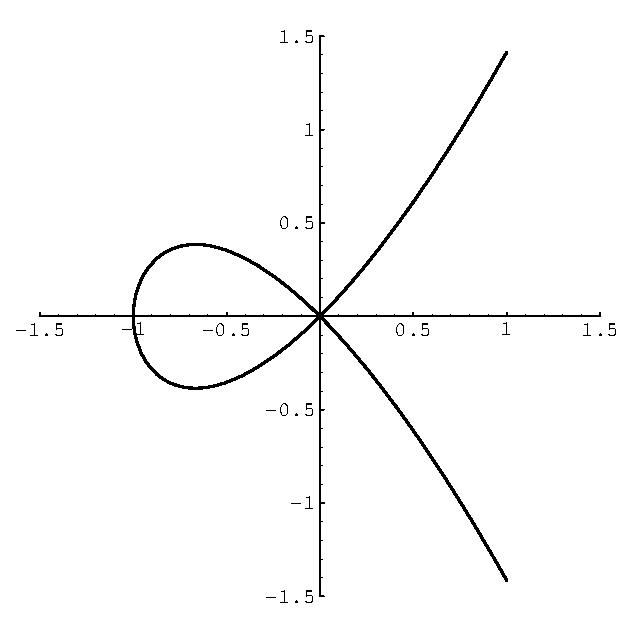
\includegraphics[width=2truein]{henselsg} &
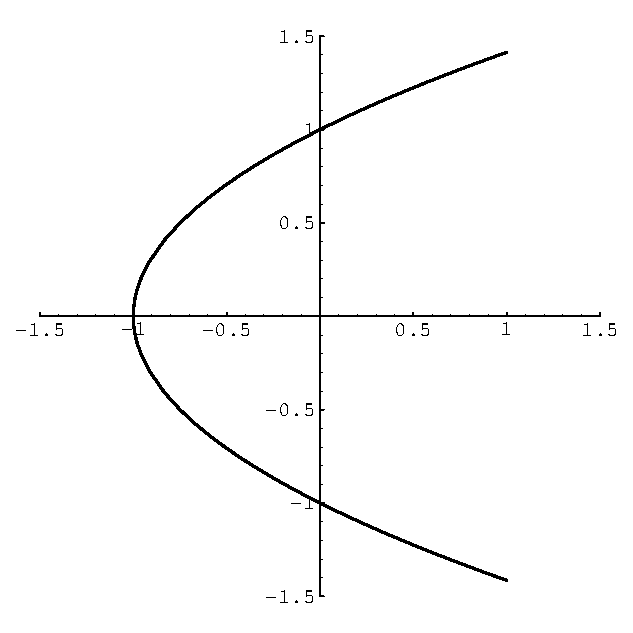
\includegraphics[width=2truein]{henselns} \\
(a) & (b)
\end{tabular}
\end{center}
\caption{The curves $Z^2 - t^3 -t^2$ and $Z^2 - t -1$
 \label{HenselSing:Fig}}
\end{figure}

As an example of what occurs when the derivative vanishes, consider
the polynomial
\[
F(Z) = Z^2 - t^2 - t^3,
\]
over the field $K = \Q(t)$.  If $F(Z)$ is square free and has two
distinct zeroes in $K_{(t)} = \Q((t))$:
\[
\begin{aligned}
\alpha & = t + \frac{t^2}{2} + \frac{t^3}{8} + \cdots, \\
\beta & =  - t - \frac{t^2}{2} - \frac{t^3}{8} - \cdots.
\end{aligned}
\]
However, modulo $\mathfrak{m} = (t)$ $F(Z)$ is not square free since the
constant terms of $\alpha$ and $\beta$ are the same.  

This situation is described geometrically in
\figref{HenselSing:Fig}(a).  In general, there are two points on the 
curve of $Z^2 - t^2 - t^3$ lying above any point on the horizontal,
$t$ axis.  At $t=0$ however, these two curve segments come together
at, what is called a \keyi{singular point} of the algebraic curve.

We can {\em desingularize} the curve at $t=0$, by focusing on the
second term in the power series expansion of $\alpha$ and $\beta$ not
the first.  That is, we replace $Z$ by $t Z'$.  This gives the new
equation:
\[
t^2 {Z'}^2 - t^2 -t^3 = 0.  
\]
So we can replace $F(Z)$ by $G(Z') = {Z'}^2 - 1 -t$.  This polynomial does
not have repeated roots modulo $\mathfrak{m}$ as is clear from
\figref{HenselSing:Fig}(b). 

More generally, assume that we have a polynomial $F(Z)$ over a ring
$R$ that is square free, but where $F(Z)$ is not square free over
$R/\mathfrak{p}$.  Further, assume that $\mathfrak{p} = (p)$ is a principal
ideal.  Since $F(Z)$ is not square free, it has more than one zero
lying over the point $\mathfrak{p}$ but which agree modulo $\mathfrak{p}$,
\eg,
\[
\begin{aligned}
\alpha & = a_0 + a_1 p + a_2 p^2 + a_3 p^3 + \cdots, \\
\beta  & = a_0 + b_1 p + b_2 p^2 + b_3 p^3 + \cdots.
\end{aligned}
\]
We can desingularize $F$ by using the new polynomial
\[
\frac{1}{p} F(p(Z - a_0))
\]
in place of $F(Z)$.  

The transformation described in the previous paragraph is called a
\keyi{blow up}.  It is known that blowup type transformations are
sufficient for desingularizing algebraic 
curves.\index{desingularization}  By repeatedly 
performing ``blow ups'' we can separate zeroes that agree modulo
$\mathfrak{p}^k$ for arbitrarily large, but finite $k$.  We can then
apply Newton's method to the desingularized equation to produce
approximations to the roots of arbitrary order.  

Note that if $F(Z)$ is not square free over $R$ then it is never
possible to separate the zeroes.

\section{Multidimensional Iteration}
\label{Multivariate:Newton:Sec}

Just as in the single variable case, the multivariate version of
Newton's iteration begins with \key{Taylor's formula}, this time in several
variables: Let $f(Z_1, \ldots, Z_n)$ be a polynomial in the variables
$Z_1, \ldots, Z_n$.  Its Taylor series expansion at $(x_1,\ldots,
x_n)$ is
\begin{equation}\label{Hensel:8}
\begin{aligned}
  \multispan{1}{$f(Z_1,\ldots, Z_n)$}\\
    \qquad = f(x_1,\ldots, x_n) &\null + 
    \sum_{i=1}^n {\partial f \over \partial Z_i}(x_1,\ldots,x_n) 
    (Z_i - x_i)\\
   & + {1 \over 2} \sum_{i=1}^n \sum_{j=1}^n
    {\partial^2 f \over \partial Z_i \, \partial Z_j}(x_1,\ldots,x_n) 
    (Z_i - x_i) (Z_j - x_j)\\
   & + \cdots\\
\end{aligned}
\end{equation}

The first summation in equation \eqnref{Hensel:8} is the inner product
of the row vector
\[
{\partial f \over \partial \vec{Z}} (\vec{x}) =
\left({\partial f \over \partial Z_1} (\vec{x}), 
{\partial f \over \partial Z_2} (\vec{x})
\ldots, {\partial f \over \partial Z_n} (\vec{x}) \right).
\]
and the column vector
\[
(\vec{Z} - \vec{x}) = \begin{pmatrix}Z_1 - x_1\\ \vdots\\ Z_n - x_n\end{pmatrix},
\]
where we have used $\vec{x}$ as an abbreviation for $(x_1, x_2, \ldots,
x_n)$ as in \sectref{Poly:Generalities:Sec}.  Using this notation, the
first two terms of \key{Taylor's formula} can be expressed as
\[
f(\vec{Z} ) = f(\vec{x}) + {\partial f \over \partial \vec{Z}}
(\vec{x}) \cdot (\vec{Z}  - \vec{x}) + \cdots.
\]

More generally, let $R$ be commutative ring, $\mathfrak{m}$ a maximal
ideal of $R$ and $\vec{f} = (f_1,\ldots,f_m)$ be a map from $R_\mathfrak{
m}^n$ to $R_\mathfrak{m}^m$.  It can be locally represented as a
multivariate power series expansion at $\vec{x}$
\[
\vec{f} (\vec{Z}) = \vec{f}(\vec{x}) 
  + \mathbf{J}(\vec{x})\cdot(\vec{Z} - \vec{x}) 
  + \cdots
\]
where $\mathbf{J}(\vec{x})$ is the \keyi{Jacobian} of the map $\vec{f}$:
\[
\mathbf{J}(\vec{x}) = 
\frac{\partial \vec{f}}{\partial \vec{Z}}
=
\begin{pmatrix}{\partial f_1\over \partial Z_1}& {\partial f_1\over \partial Z_2}&
 \cdots&{\partial f_1\over \partial Z_n}\\
{\partial f_2\over \partial Z_1}& {\partial f_2\over \partial Z_2}&
 \cdots&{\partial f_2\over \partial Z_n}\\
\vdots&\vdots&\ddots&\vdots\\
{\partial f_m\over \partial Z_1}& {\partial f_m\over \partial Z_2}&
 \cdots&{\partial f_m\over \partial Z_n}\end{pmatrix}.
\]
Again, letting $\vec{\alpha}$ be an element of the kernel of $\vec{f}$ and
expanding $\vec{f}$ at $\vec{\alpha} - \vec{\alpha}^{(k-1)}$, we have
\begin{equation}
0 = \vec{f}(\vec{\alpha}^{(k-1)}) + \mathbf{J}(\vec{\alpha}^{(k-1)}) 
\cdot (\vec{\alpha}  - \vec{\alpha}^{(k-1)}) +
O\left((\vec{\alpha} - \vec{\alpha}^{(k-1)})^{2}\right).
\label{MNewton:1:Eq}
\end{equation}

The term $O\left((\vec{\alpha} - \vec{\alpha}^{(k-1)})^{2}\right)$ is an
element of $\mathfrak{m}^{2}$.  If the rank of the Jacobian matrix is $n$
then the coordinates are well determined.  Choosing those rows of
\eqnref{MNewton:1:Eq} that are independent gives
\begin{equation}\label{MNewton:2:Eq}
\vec{\alpha}^{(2k-1)} - \vec{\alpha}^{(k-1)} 
  = -\mathbf{J}(\vec{\alpha}^{(k-1)})^{-1} 
  \cdot \vec{f}(\vec{\alpha}^{(k-1)}), \pmod{\mathfrak{m}^{2k}}
\end{equation}
which is quite similar to the quadratically convergent univariate iteration
\eqnref{Basic:UNewton:Eq}.  Equation \eqnref{MNewton:2:Eq} permits us to 
compute the element of 
$(R_\mathfrak{m})^n$ that lies over $\vec{\alpha_0}$.  However, this iteration
requires a matrix inversion at each step using a quadratically convergent 
iteration.  One way to eliminate the repeated matrix inversions is to use 
a linearly convergent version of \eqnref{MNewton:2:Eq}
\begin{equation}\label{MNewton:Lin:Eq}
\vec{\alpha}^{(k)} - \vec{\alpha}^{(k-1)}
   = -\mathbf{J}(\vec{\alpha}^{(0)})^{-1} 
  \cdot \vec{f}(\vec{\alpha}^{(k-1)}). \pmod{\mathfrak{m}^{k+1}}
\end{equation}

The linearly convergent iteration constructively shows that if the
Jacobian of a system of polynomial equations is invertible, a zero of
$\vec{f}(\vec{Z})$ modulo $\mathfrak{m}$ can always be lifted to a zero
modulo $\mathfrak{m}^k$ for any $k$.  That is,

\begin{proposition}\label{MNewton:Iter:Prop}
Assume $R$ is an integral domain with an ideal $\mathfrak{m}$.  Let
$\vec{f} = (f_1(Z_1, \ldots, Z_n), \ldots, f_n(Z_1, \ldots, Z_n))$ be
polynomials over $R$ and denote their Jacobian with respect to the
$Z_i$ by $\mathbf{J}$.  Let $(x_1, \ldots, x_n)$ be a zero of $\vec{f}$
modulo $\mathfrak{m}$ such that the determinant of $\mathbf{J}(x_1, \ldots,
x_n)$ has an inverse in $R/\mathfrak{m}$.  Then there exist unique
elements $\hat{x}_1, \ldots, \hat{x}_n$ of $R_\mathfrak{m}$, $\hat{x}_i =
x_i \mod\mathfrak{m}$, for which $\vec{f}(\hat{x}_1, \ldots, \hat{x}_n)
= 0$.
\end{proposition}

\begin{proof}
Let $\alpha_i^{(0)} = x_i$.  Since $\mathbf{J}(x_1, \ldots, x_n)$ is
invertible modulo $\mathfrak{m}$ we can repeatedly apply
\eqnref{MNewton:Lin:Eq} to compute $\vec{\alpha}^{(k)}$ for any
$k$.  The $\vec{\alpha}_i^{(k)}$ form a \key{coherent sequence} whose
limit is $\hat{x}_i$.

Thus there exists a point $(\hat{x}_1, \ldots, \hat{x}_n)$ that
satisfies the conditions of the proposition.  Assume that $(\hat{y}_1, 
\ldots, \hat{y}_n)$ also satisfies the proposition and that $k$ is the 
smallest value for which 
\begin{equation} \label{MNewton:NotEq:Eq}
\hat{x}_i \not= \hat{y}_i \pmod{\mathfrak{m}^{k+1}}
\end{equation}
for some $i$. Note that $k$ must be positive. We can denote by
$\vec{\alpha}^{(k-1)}$:
\[
(\hat{x}_1, \ldots, \hat{x}_n) = (\hat{y}_1, \ldots, \hat{y}_n) =
\vec{\alpha}^{(k-1)} \pmod{\mathfrak{m}^k}
\]
But then we have:
\[
\begin{aligned}
(\hat{x}_1, \ldots, \hat{x}_n) - \vec{\alpha}^{(k-1)}
   &= -\mathbf{J}(\vec{\alpha}^{(0)})^{-1} 
  \cdot \vec{f}(\vec{\alpha}^{(k-1)}), \\
(\hat{y}_1, \ldots, \hat{y}_n) - \vec{\alpha}^{(k-1)}
   &= -\mathbf{J}(\vec{\alpha}^{(0)})^{-1} 
  \cdot \vec{f}(\vec{\alpha}^{(k-1)}),
\end{aligned}
\pmod{\mathfrak{m}^{k+1}}
\]
which contradicts \eqnref{MNewton:NotEq:Eq}.
\end{proof}

\paragraph{Quadratic Iteration}

The need to repeatedly invert the Jacobian of the system can also be 
eliminated by applying Newton's method to the equation for the reciprocal 
of the Jacobian as described was done in
\sectref{Univariate:Newton:Sec}.\Marginpar{Rewrite this paragraph}
We apply \eqnref{MNewton:2:Eq} to the system linear of equations
\[
\mathbf{X} \cdot \mathbf{J}(\alpha) = {\bf 1}
\]
where both $\bf X$ and $\bf 1$ are $n\times n$ matrices, and the
components of $\bf X$ are to be determined.  Given
$\mathbf{\Upsilon}^{(k-1)}$ such that 
\[
\mathbf{\Upsilon}^{(k-1)} \cdot \mathbf{J}(\vec{\alpha}) = 
\mathbf{\Upsilon}^{(k-1)} \cdot \mathbf{J}(\vec{\alpha}^{(2k-1)}) = {\bf 1},
  \pmod{\mathfrak{m}^{k}}
\]
we want to find $\mathbf{\Upsilon}^{(2k-1)}$ where
\begin{equation} \label{Jacobian:1:Eq}
\mathbf{\Upsilon}^{(2k-1)} \cdot \mathbf{J}(\alpha^{(2k-1)}) = {\bf 1} \pmod{\mathfrak{m}^{2k}}
\end{equation}
We interpret the matrix equation \eqnref{Jacobian:1:Eq} as system of 
$n^{2}$ linear equations in $n^{2}$ unknowns, where the unknowns are the 
entries of $\mathbf{\Upsilon}^{(2k-1)}$. 

The Jacobian of \eqnref{Jacobian:1:Eq} is a block diagonal
$n^{2}\times n^{2}$ matrix, where each block contains
$\mathbf{J}(\alpha^{(2k-1)})^{T}$.  Since we only need to compute the
inverse of this matrix modulo $\mathfrak{m}^{k}$, we can write its
inverse as
\[
\begin{aligned}
\begin{pmatrix}
 \mathbf{J}(\alpha^{(2k-1)})^T & {\bf 0} & \cdots & {\bf 0}\\
 {\bf 0} & \mathbf{J}(\alpha^{(2k-1)})^T & \cdots & {\bf 0} \\
 \vdots  & & & \vdots \\
 {\bf 0} & {\bf 0} & \cdots & \mathbf{J}(\alpha^{(2k-1)})^T \end{pmatrix}^{-1} \qquad\\
 = 
\begin{pmatrix}
 \mathbf{\Upsilon}^{(k-1) \, T} & {\bf 0} & \cdots & {\bf 0}\\
 {\bf 0} & \mathbf{\Upsilon}^{(k-1) \, T} & \cdots & {\bf 0} \\
 \vdots  & & & \vdots \\
 {\bf 0} & {\bf 0} & \cdots & \mathbf{\Upsilon}^{(k-1) \, T} \end{pmatrix}
\end{aligned}
\pmod{\mathfrak{m}^{k}}
\]
According to \eqnref{MNewton:2:Eq}, $\vec{\mathbf{J}}^{(2k-1)} - \vec{\mathbf{J}}^{(k)}$
is equal to the product of this matrix multiplied on the right by the
vector of entries of 
\[
\mathbf{\Upsilon}^{(k-1)} \cdot \mathbf{J}(\alpha^{(2k-1)}) - {\bf 1} \pmod{\mathfrak{m}^{2k}}.
\]
Due to the repetitive structure of the Jacobian, we can write this as 
\begin{equation}
\mathbf{\Upsilon}^{(2k-1)} - \mathbf{\Upsilon}^{(k-1)} =
({\bf 1} - \mathbf{\Upsilon}^{(k-1)} \cdot \mathbf{J}(\vec{\alpha}^{(2k-1)})) \cdot 
\mathbf{\Upsilon}^{(k-1)} \pmod{\mathfrak{m}^{2k}}
\label{MNewton:3:Eq}
\end{equation}

Putting this together with \eqnref{MNewton:2:Eq} we have
\begin{equation}
\label{Quasi:MNewton:Eq}
 \begin{aligned}
   \vec{\alpha}^{(2k-1)} - \vec{\alpha}^{(k-1)} & 
      = -\mathbf{\Upsilon}^{(k-1)}\cdot \vec{f}(\vec{\alpha}^{(k-1)}) \\
   \mathbf{\Upsilon}^{(2k-1)} - \mathbf{\Upsilon}^{(k-1)} &=
     ({\bf 1} - \mathbf{\Upsilon}^{(k-1)} \cdot \mathbf{J}(\vec{\alpha}^{(2k-1)})) 
          \cdot \mathbf{\Upsilon}^{(k-1)}
 \end{aligned}
 \pmod{\mathfrak{m}^{2k}}
\end{equation}
which is the basic quadratically convergent multivariate iteration.

To illustrate the steps leading from \eqnref{Jacobian:1:Eq} to
\eqnref{MNewton:3:Eq}, we consider the $2 \times 2$ case explicitly:
\[
\begin{aligned}
\mathbf{X}^{(2k-1)} \cdot \mathbf{M}^{(2k-1)} 
& = 
\begin{pmatrix}x_{11}^{(2k-1)} & x_{12}^{(2k-1)} \\\noalign{\vskip3pt}
x_{21}^{(2k-1)} & x_{22}^{(2k-1)} \end{pmatrix} 
\cdot
\begin{pmatrix}m_{11}^{(2k-1)} & m_{12}^{(2k-1)} \\\noalign{\vskip3pt}
m_{21}^{(2k-1)} & m_{22}^{(2k-1)} \end{pmatrix} \\
& = \begin{pmatrix}1& 0 \\ 0 & 1 \end{pmatrix},
\end{aligned}
\pmod{\mathfrak{m}^{2k}}
\]
where $\mathbf{M}^{(2k-1)}$ is the image modulo $\mathfrak{m}^{2k}$ of a
known matrix $\mathbf{M}$ and $\mathbf{X}^{(2k-1)}$ is a matrix whose elements
are to be determined.  The correspondence to our case is
$\mathbf{X}^{(2k-1)} = \mathbf{\Upsilon}^{(2k-1)}$ and $\mathbf{M}^{(2k-1)} =
\mathbf{J}(\vec{\alpha}^{(2k-1)})$. In terms of their components, these
equations are 
\[
\begin{aligned}
 f_1(x_{11}, x_{12}, x_{21}, x_{22}) & 
   = m_{11} x_{11} + m_{21} x_{12} - 1, \\
 f_2(x_{11}, x_{12}, x_{21}, x_{22}) & 
   = m_{12} x_{11} + m_{22} x_{12}, \\ 
 f_3(x_{11}, x_{12}, x_{21}, x_{22}) & 
   = m_{11} x_{21} + m_{21} x_{22}, \\ 
 f_4(x_{11}, x_{12}, x_{21}, x_{22}) & 
   = m_{12} x_{21} + m_{22} x_{22} - 1,
\end{aligned}
\]
which gives a Jacobian of 
\[
\begin{pmatrix}
   m_{11} & m_{21} & 0 & 0 \\
   m_{12} & m_{22} & 0 & 0 \\
   0 & 0 & m_{11} & m_{21} \\
   0 & 0 & m_{12} & m_{22} \end{pmatrix}.
\]
Using \eqnref{MNewton:2:Eq}, the quadratic iteration for the solution
of this system of equations is
\[
\begin{aligned}
\null & \begin{pmatrix}
  x_{11}^{(2k-1)} - x_{11}^{(k-1)} \\
  x_{12}^{(2k-1)} - x_{12}^{(k-1)} \\
  x_{21}^{(2k-1)} - x_{21}^{(k-1)} \\
  x_{22}^{(2k-1)} - x_{22}^{(k-1)} \end{pmatrix} \\
\null & \qquad =
- \begin{pmatrix}
   j_{11}^{(k-1)} & j_{21}^{(k-1)} & 0 & 0 \\
   j_{12}^{(k-1)} & j_{22}^{(k-1)} & 0 & 0 \\
   0 & 0 & j_{11}^{(k-1)} & j_{21}^{(k-1)} \\
   0 & 0 & j_{12}^{(k-1)} & j_{22}^{(k-1)} \end{pmatrix}
\cdot
\begin{pmatrix}
  f_1(\vec{x}^{(k-1)}) \\ 
  f_2(\vec{x}^{(k-1)}) \\
  f_3(\vec{x}^{(k-1)}) \\ 
  f_4(\vec{x}^{(k-1)}) \end{pmatrix} \\
\null & \qquad = - \begin{pmatrix}
    j_{11}^{(k-1)}f_1(\vec{x}^{(k-1)}) + j_{21}^{(k-1)}f_2(\vec{x}^{(k-1)})\\
    j_{12}^{(k-1)}f_1(\vec{x}^{(k-1)}) + j_{22}^{(k-1)}f_2(\vec{x}^{(k-1)})\\
    j_{11}^{(k-1)}f_3(\vec{x}^{(k-1)}) + j_{21}^{(k-1)}f_4(\vec{x}^{(k-1)})\\
    j_{12}^{(k-1)}f_3(\vec{x}^{(k-1)}) + j_{22}^{(k-1)}f_4(\vec{x}^{(k-1)})
    \end{pmatrix}
\\
\end{aligned}
\pmod{\mathfrak{m}^{2k}}
\]
This can be rewritten as a product of $2 \times 2$ matrices as 
\[
\begin{aligned}
\null & \begin{pmatrix}
  x_{11}^{(2k-1)} - x_{11}^{(k-1)} &
  x_{12}^{(2k-1)} - x_{12}^{(k-1)} \\
  x_{21}^{(2k-1)} - x_{21}^{(k-1)} &
  x_{22}^{(2k-1)} - x_{22}^{(k-1)} \end{pmatrix} \\
\null & \qquad =
\begin{pmatrix}
  f_1(\vec{x}^{(k-1)}) & f_2(\vec{x}^{(k-1)}) \\
  f_3(\vec{x}^{(k-1)}) & f_4(\vec{x}^{(k-1)}) \end{pmatrix}
\cdot
\begin{pmatrix}
   j_{11}^{(k-1)} & j_{12}^{(k-1)} \\
   j_{21}^{(k-1)} & j_{22}^{(k-1)} \end{pmatrix}
\end{aligned}
\]


The initial solution of the system of equations, $\vec{\alpha}_{0}$ is
called the starting point of the iteration.  If
$\mathbf{J}(\vec{\alpha}_0)$ is invertible then $\vec{\alpha}_0$ is said
to be a \keyi{good starting point}.  If the Jacobian matrix is not
invertible, either because the $\vec{\alpha}_0$ was a bad starting
point or because the Jacobian itself was not square, then the system
of linear equations that need to be solved at each step will not have a
unique solution.  There are cases where this can be useful, for
instance as a sieve for possible solutions to diophantine 
equations\index{diophantine equation}
over the integers.

\section{Hensel's Lemma}
\label{Hensel:Lemma:Sec}
\index{Hensel's lemma|(}

One of the the most useful theorems in commutative algebra is {\em
Hensel's lemma}.  Essentially, it says that if a monic polynomial with
coefficients in a ring $R$ factors modulo an ideal $\mathfrak{m}$, then
it factors as a polynomial over $R_\mathfrak{m}$.  More precisely,

\begin{proposition}[Hensel's Lemma] \label{Hensel:Lemma:Prop}
Let $F(Z)$ be a monic polynomial over an integral domain $R$,
$\mathfrak{m}$ an ideal of $R$.  If there exist polynomials $G(Z)$ and
$H(Z)$ over $R/\mathfrak{m}$ such that 
\[
F(Z) = G(Z) H(Z) \pmod\mathfrak{m}
\]
and $G(Z)$ and $H(Z)$ are relatively prime as polynomials over
$R/\mathfrak{m}$, then there exist polynomials $\hat{G}(Z)$ and
$\hat{H}(Z)$ over $R_\mathfrak{m}$ such that
\[
\begin{aligned}
G(Z) & = \hat{G}(Z) \\ H(Z) & = \hat{H}(Z)
\end{aligned}
\pmod\mathfrak{m}
\]
and $F(Z) = \hat{G}(Z) \hat{H}(Z)$ over $R_\mathfrak{m}$.
\end{proposition}

Although, this proposition is phrased in terms of polynomials in $R[Z]$, 
the variable $Z$ is only used as a place holder that allows us to 
succinctly describe a system of non-linear equations.  This is clarified 
in the following proof. 

\begin{proof}
Let the degree of $F$ in $Z$ be $d$ and that of $G(Z)$ and $H(Z)$ be
$r$ and $s$ respectively, $r+s = d$.  We denote the coefficients of
$F$ by $f_i$,
\[
F(Z) = Z^d + f_1 Z^{d-1} + \cdots + f_d,
\]
where $f_i \in R$.  And the coefficients of $G$ and $H$ by $g^{(0)}_i$
and $h^{(0)}_i$:
\[
\begin{aligned}
G(Z) &= Z^r + g^{(0)}_1 Z^{r-1} + \cdots + g^{(0)}_r, \\
H(Z) &= Z^s + h^{(0)}_1 Z^{s-1} + \cdots + h^{(0)}_s,
\end{aligned}
\]
where $g^{(0)}_i$ and $h^{(0)}_i$ are elements of $R/\mathfrak{m}$.

If $G$ and $H$ can be lifted to polynomials over
$R_\mathfrak{m}$, then we can write
\[
\begin{aligned}
\hat{G}(Z) & = Z^r + g_1 Z^{r-1} + \cdots + g_r, \\
\hat{H}(Z) & = Z^s + h_1 Z^{s-1} + \cdots + h_s, 
\end{aligned}
\]
where $g_i$ and $h_i$ are unknown elements of $R_\mathfrak{m}$.
Expanding $\hat{G}(Z) \hat{H}(Z) = F(Z)$ and equating coefficients of
$Z$ we have
\begin{equation}\label{Hensel:Eq}
\begin{aligned}
  g_1 + h_1&= f_1,\\
  g_2 + g_1h_1 + h_2&= f_2,\\
  \vdots&\\
  g_r h_{s-1} + g_{r-1} h_s&= f_{n-1},\\
  g_r h_s&= f_n.
\end{aligned}
\end{equation}
This is a system of $d$ equations if $r+s$ unknowns and is called the
\keyi{coefficient equations} of the factorization $F = \hat{G}\cdot
\hat{H}$.  Any factorization of $F(Z)$ into factors of degree $r$ and
$s$ leads to a solution of \eqnref{Hensel:Eq}.  Conversely, any
solution of \eqnref{Hensel:Eq} leads to a factorization of $F(Z)$.
Thus solving \eqnref{Hensel:Eq} and factoring $F(Z)$ are equivalent. 

The coefficients of $G(Z)$ and $H(Z)$ are a solution of
\eqnref{Hensel:Eq} modulo $\mathfrak{m}$.  By \propref{MNewton:Iter:Prop} this
solution can be uniquely lifted to a solution in $R_\mathfrak{m}$ if the
Jacobian of \eqnref{Hensel:Eq} is non-singular.

The Jacobian of \eqnref{Hensel:Eq} can be computed directly:
\[
\left(
\begin{array}{cccccccc}
  1 &   0 & \ldots &   0 &   1 &   0 & \ldots & 0 \\
h_1 &   1 &        &   0 & g_1 &   1 &        & 0 \\
h_2 & h_1 & \ldots &   0 & g_2 & g_1 & \ldots & 0 \\
\vdots&   &        &     & \vdots&   &        &\vdots\\
0   &   0 & \ldots & h_s & 0   &   0 & \ldots &g_r
\end{array}
\right),
\]
the \key{Sylvester matrix} for the \key{resultant} of $G(Z)$ and
$H(Z)$, as was pointed out in \sectref{Poly:Resultant:Sec}.  It is
known to be zero if and only if $g$ and $h$ have a nontrivial common
factor.  Since $G(Z)$ and $H(Z)$ are assumed to be relatively prime,
the Jacobian is always non-singular.
\end{proof}

\paragraph{Example}

Consider the polynomial 
\[
F(Z) = Z^5 +Z^4 + 2Z^2 + 2Z + 3.
\]
Modulo $5$ it can be factored
\begin{equation}\label{Hensel:Ex5:Eq}
F(Z) = (Z^3 + 4Z + 3) (Z^2 + Z + 1) \pmod{5}
\end{equation}
Suspecting that $F(Z)$ factors into a quadratic and a cubic factor
over the rational integers we use \longpropref{Factor:CBound:Prop} to
bound the size of the coefficients of its factors.  If $G$ and $H$ are
the cubic and quadratic factors of $F$ over the integers, then
\[
(d+1)^{1/2} 2^d |F| = \sqrt{6}\, 2^5\times 3 \approx 8465 \ge \max \{
|G|, |H|\}.
\]
So we should lift the factorization of $F(Z)$ to one modulo $5^7 > 2
\times 9000$.

The \keyi{coefficient equations} corresponding to the factorization of
$F(Z)$ into a cubic and quadratic factor are
\begin{equation} \label{MNewton:Sing:Eq}
\begin{aligned}
a_1 + b_1 & = 1, \\
a_2 + a_1 b_1 + b_2 & = 0, \\
a_3 + a_2 b_1 + a_1 b_2 & = 2, \\
a_3 b_1 + a_2 b_2 & = 2, \\
a_3 b_2 & = 3.
\end{aligned}
\end{equation}
The Jacobian of this system of equations is 
\[
\left(
\begin{array}{ccccc}
1 & 0 & 0 & 1 & 0 \\
b_1 & 1 & 0 & a_1 & 1 \\
b_2 & b_1 & 1 & a_2 & a_1 \\
0   & b_2 & b_1 & a_3 & a_2 \\
0   & 0   & b_2 & 0   & a_3
\end{array}
\right).
\]
We can verify that this matrix is non-singular when the $a_i$ and
$b_i$ are replaced by their corresponding values from
\eqnref{Hensel:Ex5:Eq}.  By applying the multivariate version of Newton's
iteration \eqnref{MNewton:Lin:Eq} we get 
\[
\begin{aligned}
a_1 & = 0 + 0\cdot 5 + 0 \cdot 5^2 + 0 \cdot 5^3 + \cdots, \\
a_2 & = 6 + 6\cdot 5 + 6 \cdot 5^2 + 6 \cdot 5^3 + \cdots, \\
a_3 & = 3 + 0\cdot 5 + 0 \cdot 5^2 + 0 \cdot 5^3 + \cdots, \\
b_1 & = 1 + 0\cdot 5 + 0 \cdot 5^2 + 0 \cdot 5^3 + \cdots, \\
b_2 & = 1 + 0\cdot 5 + 0 \cdot 5^2 + 0 \cdot 5^3 + \cdots. \\
\end{aligned}
\]

Modulo $7$ however we get the factorization
\[
f(Z) = (Z^3 + 6 Z + 3) (Z^2 +  Z + 1).
\]
These factors are not irreducible and share a common factor of
$X+3$.  The Jacobian in this case is 
\[
\left(
\begin{array}{ccccc}
1 & 0 & 0 & 1 & 0 \\
1 & 1 & 0 & 0 & 1 \\
1 & 1 & 1 & 6 & 0 \\
0 & 1 & 1 & 3 & 6 \\
0 & 0 & 1 & 0 & 3
\end{array}
\right),
\]
whose integer determinant is $4 \times 7$.

\label{PolyZ7:SQFR:Ex}
Although $F(Z)$ is not square free over $\Z/(7)$ it does have three
distinct zeroes in $\Z_7$:
\[
\begin{aligned}
\alpha_1 & = 4 + 2\cdot 7 + 0\cdot 7^2 + 3\cdot 7^3 + 6\cdot 7^4 +
4\cdot 7^5 + 0\cdot 7^6 + 4\cdot 7^7 + \cdots \\
\alpha_2 & = 4 + 1\cdot7 + 3\cdot7^2 + 6\cdot7^3 + 0\cdot7^4 + 2\cdot7^5
+ 5\cdot7^6 + 1\cdot7^7 + \cdots \\
\alpha_3 & = 2 + 4\cdot7 + 6\cdot7^2 + 3\cdot7^3 + 0\cdot7^4 +
2\cdot7^5 + 6\cdot7^6 + 2\cdot7^7 + \cdots
\end{aligned}
\]
This explains the indeterminacy of the factorization.  The quadratic
factor could be either
\[
(Z - \alpha_1) \cdot (Z - \alpha_3) \quad\mbox{or}\quad
(Z - \alpha_2) \cdot (Z - \alpha_3).
\]
Both factorizations have the same image modulo $7$.  Since $7^2$ does
not divide the determinant of the Jacobian, these two factorizations
can be differentiated by their images modulo $7^2$.

The system of equations \eqnref{MNewton:Sing:Eq} describes an
algebraic surface embedded in a five dimensional space.  The fact that
the Jacobian is divisible by $7$ means that the surface has a singular
point at $(7)$.  It is possible to desingularize surface by blow ups
as described in the unvariate case,\index{desingularization} \index{blow 
up} but the discussion would take us too far a field.

\index{Hensel's lemma|)}

\section{Generalizations of Hensel's Lemma}
\label{General:Hensel:Sec}

While Hensel's lemma is usually expressed in terms of factoring a
polynomial into two relatively prime factors, the technique given in
the previous section can be applied more generally. 

Consider what happens if $F(Z)$ has three factors modulo
$\mathfrak{m}$, \ie, $F(Z) = A(Z) \cdot B(Z) \cdot C(Z)$ modulo
$\mathfrak{m}$ and $A(Z)$, $B(Z)$, and $C(Z)$ have degrees $r_1$,
$r_2$ and $r_3$ respectively, $r = r_1 + r_2 + r_3$.  We then know
that
\[
\begin{aligned}
  Z^r + \cdots + f_r&=
    (Z^{r_1} + \cdots + a_{r_{1}}) (Z^{r_2} + \cdots + b_{r_{2}})
    (Z^{r_3} + \cdots + c_{r_{3}}),\\
   &= Z^{r_1 + r_2 + r_3} + (a_{1} + b_{1} + c_{1}) Z^{r_1 + r_2 + r_3 -1} 
    + \cdots + a_{r_{1}} b_{r_{2}} c_{r_{3}}.
\end{aligned}
\]
If we equate the coefficients $Z^i$ on the right hand side of the
equation with those on the left hand side, we get a system of $r = r_1 + 
r_2 + r_3$ algebraic equations in $r$ unknowns.  The Jacobian of this 
system is a $r\times r$ matrix, $\mathbf{J}_1$ whose first $r_1$ columns 
look like 
\[
\overbrace{
\begin{array}{cccc}
1 & 0 & \cdots  & 0 \\
b_1 + c_1 & 1 & \cdots & 0\\
b_2 + b_1 c_1 + c_2 & b_1 + c_1 &  \cdots & 0 \\
\vdots & & & \vdots \\
0 & 0 & \cdots & b_{r_2} c_{r_3} \\
\end{array}}^{r_1}
\]
The next $r_2$ and $r_3$ columns are organized similarly.  By
\propref{MNewton:Iter:Prop}, when $\mathbf{J}_1$ is invertible over
$R/\mathfrak{m}$ the factorization $F = A \cdot B \cdot C$ can be lifted
{\em uniquely} to a factorization of $F$ in $R_\mathfrak{m}$.  When there
are just two factors, non-singularity of the Jacobian corresponds to
the factors being relatively prime.  What criteria corresponds to the
invertibility of $\mathbf{J}_1$?

If $A(Z)$ and $B(Z)$ are not relatively prime modulo $\mathfrak{m}$, then
the lift is certainly not unique, and similarly for the other pairings.
Thus, we expect that
\[
R = (\res_Z (A(Z), B(Z))) \cdot (\res_Z (A(Z), C(Z))) 
  \cdot (\res_Z (B(Z), C(Z)))
\]
divides the determinant of $\mathbf{J}_1$.  The term with maximum total 
degree in $R$ has total degree 
\[
(r_1 + r_2 - 1) + (r_1 + r_3 - 1) + (r_2 + r_3 - 1) = 2r -3.
\]
Examining the degrees of the rows of $\mathbf{J}_1$ we see that the monomial
of maximum total degree in 
the determinant of $\mathbf{J}_1$ has total degree
\[
0 + 1 + \overbrace{2 + 2 + \cdots + 2}^{r-2} = 2r -3.
\]
Thus,
\[
\det \mathbf{J}_1 = (\res_Z (A(Z), B(Z))) \cdot (\res_Z (A(Z), C(Z))) 
  \cdot (\res_Z (B(Z), C(Z))).
\]
Similar reasoning extends this result to an arbitrary number of
pairwise relatively prime factors.  

\smallskip
More generally, assume we have a monic polynomial $F(Z)$ over a ring
$R$ that has a factorization
\begin{equation} \label{Hensel:NSQ:Eq}
F(Z) = P_1^{e_1}(Z) \cdot P_2^{e_2}(Z) \cdots P_n^{e_n}(Z)
\pmod{\mathfrak{m}}
\end{equation}
The previous paragraphs discussed the case when the $e_i$ are equal to
$1$.  The coefficient equations of this factorization can be formed in
the same way as in the previous discussion.  Now, however, the number
equations exceeds the number unknowns.  Since there is a one to one
correspondence between factorizations $F(Z)$ of the form
\eqnref{Hensel:NSQ:Eq} and zeroes of the system of coefficient
equations, the coefficient equations must be consistent.

An interesting illustration of this approach is to lift the
factorization 
\[
\begin{aligned}
F(Z) & = Z^5 + Z^4 + 2Z^2 + 2Z + 3, \\
  & = (Z+3)^2 (Z+5) (Z^2 + 4Z+1),
\end{aligned}
\pmod{7}
\]
to a factorization over $\Z_7$.  On page \pageref{PolyZ7:SQFR:Ex} we showed that as
a polynomial over $\Z_7$ $F(Z)$ was square free.  Thus, this
factorization cannot be lifted to a factorization over $\Z_7$. Here we
show how the lifting process breaks down. possible since earlier $F(Z)$ was shown to be square free over $\Z_7$.

Assuming that
\begin{equation} \label{Hensel:NSQEx:Eq}
F(Z) =  (Z + a)^2  (Z+b) (Z^2+c_1Z+c_2)
\end{equation}
The coefficient equations are 
\[
\begin{aligned}
2a + b + c_1 & = 1, \\
a^2 + 2ab + 2 ac_1 + b c_1 + c_2 & = 0, \\
a^2 b + a^2 c_1 + 2 a b c_1 + 2 a c_2 + b c_2 & = 2, \\
a^2 b c_1 + a^2 c_2 + 2 a b c_2 & = 2, \\
a^2 b c_2 & = 3.
\end{aligned}
\]
The Jacobian of the first four equations, at $(a,b,c_1,c_2) =
(3,5,4,1)$ has integer determinant $48$.  Its inverse modulo $7$ is
\[
\left(
\begin{array}{cccc}
3 & 1 & 6 & 6 \\
4 & 0 & 3 & 4 \\
5 & 5 & 6 & 5 \\
1 & 6 & 5 & 6 
\end{array}
\right).
\]
Thus, we can uniquely lift the zero to a zero of the first four
equations in $\Z_7$:
\[
\begin{aligned}
a   & = 3 +         7 + 0 \cdot 7^2 + 6 \cdot 7^3 + 5 \cdot 7^4 + \cdots, \\
b   & = 5 + 2 \cdot 7 + 2 \cdot 7^2 + 1 \cdot 7^3 + 4 \cdot 7^4 + \cdots, \\
c_1 & = 3 + 1 \cdot 7 + 4 \cdot 7^2 + 0 \cdot 7^3 + 5 \cdot 7^4 + \cdots, \\
c_2 & = 1 + 3 \cdot 7 + 1 \cdot 7^2 + 1 \cdot 7^3 + 0 \cdot 7^4 +
\cdots.
\end{aligned}
\]
Unfortunately, this solution is not a zero of the final equation.
There the coefficient equations do not have a solution in $\Z_7$, just
as the polynomial $F(Z)$ does not have a factorization of the form
\eqnref{Hensel:NSQEx:Eq}.

\medskip
The {\sc gcd} problem can be handled in a similar manner.  Assume
we want to compute $H(Z)$, which is the {\sc gcd} of $F(Z)$ and $G(Z)$,
where $\deg F = r$, $\deg G = s$ and $\deg H = n$.  Letting $F(Z) =
A(Z) H(Z)$ and $G(Z) = B(Z) H(Z)$ we get the following system of
equations:
\[
\begin{aligned}
  a_1 + h_1 &= f_1\\
  a_2 + a_1 h_1 + h_2 &= f_2 \\
  \vdots\\
  a_{r - n} h_n & = f_r
\end{aligned} \qquad
\begin{aligned}
  b_1 + h_1 &= g_1\\
  b_2 + a_1 h_1 + h_2 &= g_2 \\
  \vdots\\
  b_{s - n} h_n & = g_r
\end{aligned}
\]
We now have $r+s$ equations, but only have $n + r -n + s - n = r + s
-n$ unknowns.  Thus, some of these equations are redundant if $F$
and $G$ actually have a unique {\sc gcd} of degree $n$.  Notice that
applying the Hensel approach to the {\sc gcd} problem gives a method
that lifts, not only $H$, but also the cofactors of $F$ and 
$G$.\index{cofactor} 

\section{Zassenhaus' Formulation of Hensel's Lemma}
\label{Zassenhaus:Formulation:Sec}

{\Zassenhaus}' version of \key{Hensel's lemma} differs from the one
discussed in the preceding sections in that the number of equations
produced is smaller than the number of variables.  For instance, in
the factoring problem, the Zassenhaus approach determines $G$ and $H$
by solving the equation
\begin{equation}
 \label{Zassen:Factor:Eq}
F(X) - G(X) \cdot H(X) = 0
\end{equation}
It is only when the solution of this equation is restricted to the ring
$\Z_{p}[X]$ that \eqnref{Zassen:Factor:Eq} has a unique solution.  By using
a $p$-adic technique the non-linear diophantine equation
\eqnref{Zassen:Factor:Eq} can be reduced to a series of easy to solve,
linear equations.  Then by piecing together the solutions of these linear
equations, $G$ and $H$ can be determined.  Here we outline the main 
points and demonstrate the connection with our formalism.

Let $F(X)$ be a univariate polynomial over the integers, and assume
that it has two irreducible factors, $G$ and $H$.  We are given a
factorization $F(X) = G_0 H_0$ modulo $p$ and we want to lift $G_0$
and $H_0$ to $G$ and $H$.  Writing $G$ and $H$ $p$-adically gives
\[
\begin{aligned}
  F(X) &= (G_0 + G_1 p + \cdots) (H_0 + H_1 p + \cdots), \\
   &= G_0 H_0 + (H_1 G_0 + G_1 H_0) p + \cdots.
\end{aligned}
\]
Modulo $p^2$ we have
\[
F(X) - G_0 H_0 = (H_1 G_0 + G_1 H_0) p \pmod{p^2}
\]
Since $F(X) - G_0 H_0$ is a multiple of $p$, dividing by $p$ gives 
\begin{equation}
H_1 G_0 + G_1 H_0 = \left( F(X) - G_0 H_0 \right) / p \qquad\pmod{p}
\label{Linear:Dio:Eq}
\end{equation}
This is a polynomial valued linear diophantine equation\index{diophantine 
equation!linear} in $G_1$ and $H_1$.  Its solution can be obtained by 
first solving $A_i G_0 + B_i H_0 = X^i \pmod{p}$ for various $i$ by the 
Euclidean algorithm.  Since the left hand side of \eqnref{Linear:Dio:Eq} 
is a polynomial in $X$, $G_1$ and $H_1$ can be determined by adding 
combinations of the appropriate $B_i$ and $A_i$ respectively.

Having computed $G_1$ and $H_1$, the other terms may be computed
similarly.  For a linear iteration, the process continues as follows:
\[
F(X) = (G_0 + G_1 p + G_2 p^2 + \cdots) 
(H_0 + H_1 p + H_2 p^2 + \cdots)
\]
Considering this equation modulo $p^3$
\[
(H_2 G_0 + G_2 H_0) = \left( F(Z) - 
  (G_0 + G_1 p)(H_0 + H_1 p) \right) / p^2 \qquad \pmod{p}
\]
The right hand side of this equation is again a polynomial and the
left hand side is essentially the same as \eqnref{Linear:Dio:Eq}.  So
using the $A_i$ and $B_i$ obtained in the previous step we can compute
$G_2$ and $H_2$.

\paragraph{Relation to Solving Equations}

The {\Zassenhaus} version of \key{Hensel's lemma} produces the same 
answer as the approach based on Newton's method discussed earlier---the 
correct factorization through each of the lifting stages.  The
following paragraphs demonstrate that this is not a fortuitous
accident but is due to the fact that both formulations are performing
the same computation in a slightly different manner.

The key to using {\Zassenhaus}'s formulation of \key{Hensel's lemma} to 
lift a factorization $F = G_0 H_0 \mod{\mathfrak{m}}$ to the $\mathfrak{
m}$-adic completion is solving the diophantine equations
\begin{equation} \label{Hensel:ZassDio:Eq}
A_i G_0 + B_i H_0 = Z^i \qquad\pmod{\mathfrak{m}}
\end{equation}
Once we have obtained the $A_i$ and $B_i$, it is merely a matter of
computing the error introduced when a factorization modulo $\mathfrak{m}^k$ 
is lifted to one modulo $\mathfrak{m}^{k+1}$.
This error is then used to produce the appropriate linear combination of the
$A_i$ and $B_i$ that is $G_{k+1}$ and  $H_{k+1}$.

Our formulation is quite similar.  We begin by inverting the Jacobian
matrix.  Through the Newton-Raphson formula we combine the error terms
to compute $G_{k+1}$ and $H_{k+1}$.  Structurally, these two algorithms 
are quite similar.  We shall see that the solutions of 
\eqnref{Hensel:ZassDio:Eq} form the inverse of the Jacobian matrix.

To see this let,
\[
\begin{aligned}
  G_0 &= Z^r + g_1 Z^{r-1} + g_2 Z^{r-2} + \cdots + g_r\\
  H_0 &=Z^s + h_1 Z^{s-1} + h_2 Z^{s-2} + \cdots + h_s
\end{aligned}
\]
so the Jacobian matrix is
\[
J = 
\begin{pmatrix}
1&0&0& \cdots&0&1&0&0&\cdots&0\\
h_1&1&0& \cdots&0&g_1&1&0&\cdots&0\\
h_2&h_1&1& \cdots&0&g_2&g_1&1&\cdots&0\\
\vdots&\null&\vdots&\null&\null&\vdots&\null&\vdots&\null&\vdots\\
0&\cdots&0&h_s&h_{s-1}&0&\cdots&0&g_r&g_{r-1}\\
0&\cdots&0&0&h_s&0&\cdots&0&0&g_r
\end{pmatrix}
\]
Consider what happens when this matrix is multiplied by a column vector
\[
J\cdot
\begin{pmatrix}
b_0\\ \vdots \\ b_{s-1}\\ a_0\\ \vdots\\ a_{r-1}
\end{pmatrix}
=
\begin{pmatrix}
a_0 +b_0\\
a_0 g_1 + a_1 + b_1 + b_0 h_1\\
\vdots\\
a_{r-1} g_{r-1} + a_{r-2} g_r + b_{s-2} h_{s} + b_{s-1} h_{s-1}\\
a_{r-1} g_{r} + b_{s-1} h_{s}
\end{pmatrix}
\]
The $(r+ s - 1) - i$ row of this column vector is clearly the coefficient
of $Z^i$ in $A G_0 + B H_0$ where
\[
\begin{aligned}
  A &= a_0 Z^{s-1} + a_1 Z^{s-2} + \cdots + a_{s-1},\\
  B &= b_0 Z^{r-1} + b_1 Z^{r-2} + \cdots + b_{r-1}.
\end{aligned}
\]
Thus the computation of the inverse of the Jacobian of the system of
equations is a clever way of obtaining all the solutions of
\eqnref{Hensel:ZassDio:Eq}.  Or, solving
\eqnref{Hensel:ZassDio:Eq} is a clever way of inverting a very special
type of Jacobian matrix.

\section*{Notes}

\small

\notesectref{Univariate:Newton:Sec}  Equation
\eqnref{Basic:UNewton:Eq} is a discrete version of the Newton-Raphson
iteration used in numerical analysis.  Unlike the numerical situation,
notice that convergence in the discrete case is is not an issue.  The
linearly convergent iteration \eqnref{Modified:UNewton:Eq} is called a
\keyi{modified Newton's method} in numerical analysis.

An alternative approach to Hensel's lemma liftings, but based on the
use of idempotents is given in the work of {\Gianni}, {\MillerV} and
{\Trager} \cite{Gianni88b}.

\notesectref{Multivariate:Newton:Sec} In a certain sense this is a
discrete version of a \keyi{quasi-Newton iteration}, since it updates
the Jacobian at each step rather than recomputing it.  However, most
of the numerical quasi-Newton formulas do not update the entire matrix
as is done in \eqnref{MNewton:2:Eq}.

\notesectref{Hensel:Lemma:Sec} A result equivalent to Hensel's lemma
was first proven in \cite{Hensel04,Hensel05a}.  It was given in the
form of \propref{Hensel:Lemma:Prop} in \cite{Hensel18}.

\notesectref{Zassenhaus:Formulation:Sec}  The ``old'' version of
\key{Hensel's lemma} was first proposed by {\Zassenhaus} 
\cite{Zassenhaus:Factoring:I}.  {\WangP} and {\Rothschild}
\cite{Wang75} and {\Musser} \cite{Musser75} utilized
{\Zassenhaus}' ideas in their factoring algorithm.  Using the ideas of
{\MosesJ} and {\Yun} \cite{Moses:Yun}, {\Yun}
\cite{Yun:Thesis,Yun:padic} investigated the applicability of
\key{Hensel's lemma} to problems in algebraic manipulation.

\normalsize

%$Id: /usr/u/rz/AMBook/RCS/hensel.tex,v 1.1 1992/05/10 19:42:11 rz Exp rz $
\chapter{Sparse Hensel Algorithms}
\label{Sparse:Hensel:Chap}

The last chapter gave the framework for the type of Hensel method we
will use for polynomial factorization problems.  This chapter
discusses a slight modification of the Hensel technique that allows us
to take advantage of sparsity in the problem.  The key idea used is
the same as that of sparse interpolation.  Based on some preliminary
computation, the skeleton of the answer polynomial is developed.  From
then on, it is only necessary to reconstruct the coefficients of
those monomials that actually appear in the skeleton.  In the Hensel
approach this means that when proceeding from one stage to another,
certain unknowns will be assumed to be zero and can be omitted when
constructing the system of equations.

The univariate factorization problem discussed in the
\sectref{Hensel:Lemma:Sec} gives a succinct illustration of some of
the ideas.  Assume we want to lift the factorization
\[
\begin{aligned}
F(Z) & = Z^5 + Z^4 + 2Z^2 + 2Z + 3, \\
 & = (Z^3 + 4 Z + 3) (Z^2 + Z + 1) \pmod{5}.
\end{aligned}
\]
Using the method described in the last chapter, we form the
coefficient equations for a factorization of $F$:
\[
F(Z) = (Z^3 + a_1 Z^2 + a_2 Z + a_3) (Z^2 + b_1 Z + b_2).
\]
However, to take advantage of sparsity we assume that the
coefficient of $Z^2$ in the cubic factor is zero, not only modulo $5$,
but also over $\Z_5$.  We then form the coefficient equations of 
\begin{equation} \label{SPH:Mod5:Ex}
f(Z) = (Z^3 + a_1 Z + a_2) (Z^2 + b_1 Z + b_2).
\end{equation}
That is,
\begin{equation} \label{SPM:5Coef:Eq}
\begin{aligned}
b_1 & = 1, \\
a_1 + b_2 & = 0,\\
a_2 + b_1 a_1 & = 2, \\
a_1 b_2 + a_2 b_1 & = 2, \\
a_2 b_2 & = 3.
\end{aligned}
\end{equation}

Even though there are no repeated factors in \eqnref{SPM:5Coef:Eq},
notice that there are more equations than unknowns.  The Jacobian of
this system is
\[
\left(
\begin{array}{cccc}
0 & 0 & 1 & 0 \\
1 & 0 & 0 & 1 \\
b_1 & 1 & a_0 & 0 \\
b_2 & b_1 & a_2 & a_1 \\
0 & b_2 & 0 & a_2 
\end{array}\right),
\]
which is a sub-array of the Sylvester matrix.  The determinant of the
first four rows is
\[
a_1 + b_1^2 - b_2,
\]
which is equal to $4$ modulo $5$.  So, we can apply Newton's method to 
lift $(a_1, a_2, b_1, b_2) = (4,3,1,1)$ to a zero in $\Z_5$ of the first 
four equations.  If this solution also satisfies $a_2 b_2 = 3$ then we 
have lifted the factorization of $F(Z)$ to one over $\Z_5$.

There are two interesting things to note here.  First, since we are
dealing with a smaller system of equations than with the full
Newton's method, less computation should be required.  In fact the
size of the system of equations depends on the size of the
factorization and not the degrees of the variables.

Second, these equations can be solved directly, thus giving the 
factorization of $F(Z)$ without any Hensel stages.  The first equation 
immediately gives $b_1 = 1$.  The second equation can be solved for 
$b_2$, giving $b_2 = - a_1$.  Substituting these values into the 
remaining three equations gives 
\[
\begin{aligned}
a_1 + a_2 & = 2, \\
-a_1^2 + a_2 &= 2, \\
-a_1 a_2 & = 3.
\end{aligned}
\]

Again the first of these equations is linear, so we can write $a_2 = 2
- a_1$.  Substituting this value into the last two equations gives
\[
\begin{aligned}
-a_1^2 + (2 - a_1) & = 2 \quad \Rightarrow \quad a_1^2 + a_1 = 0, \\
-a_1(2 - a_1) &= 3 \quad \Rightarrow \quad a_1^2 - 2a_1 - 3 = 0. \\
\end{aligned}
\]
The only common solution to these two equations is $a_1 = -1$, so we
have\Marginpar{Check these solutions}
\begin{alignat*}{2}
a_1 & = -1, & b_1 & = 1, \\
a_2 & = 3, & b_2 & = 1.
\end{alignat*}

\noindent
This type of situation occurs frequently with multivariate
factorizations.

Although this approach worked well in this simple problem, sparse
techniques are not often used when lifting a solution modulo a prime
number to a solution over $\Z$.  It is more effective for multivariate 
polynomial problems and we restrict our further discussion to this case.

In \sectref{SPH:Heuristic:Sec} we give an example of the use of the
sparse Hensel algorithm to solve a small system of algebraic equations
over a polynomial ring.  A more formal presentation of the algorithm
and its costs is given \sectref{SPH:Formal:Sec}.

\section{Heuristic Presentation}
\label{SPH:Heuristic:Sec}

The number and types of variables that occur in the sparse Hensel
algorithm can be bewildering.  As much as possible, we have tried to
use symbols in much the same way as was done in the discussion of
interpolation in the earlier chapters.  We always work over a ring $R = 
K[X_1, \ldots, X_v]$ and the objects of our computation are elements of 
$R$.  Our problem however is to solve a system of equations.  The 
solution of this system lie in $R$, but the equations themselves are 
polynomials in $R[\Xi_1, \ldots, \Xi_m]$. In the course of the solution, 
we convert this system of equations into a new system.  The unknowns in 
the new system are always written as $\Lambda_i$'s.

We begin with a simple example to illustrate the issues involved in
the sparse Hensel approach:
\begin{equation} \label{SPH:2var:Eq}
\begin{aligned}
\Xi_1 \Xi_2 & = X_1^6 - X_2^4, \\
\Xi_1^2 + \Xi_2^2 & = 2X_1^6 + 2X_2^4,
\end{aligned}
\end{equation}
over the ring $R = \Q[X_1, X_2]$.  $\Xi_1$ and $\Xi_2$ are assumed to be
elements of $\Q[X_1, X_2]$ of degree less than or equal to $6$ in each
variable.   

The approach of the last chapter suggests choosing the ideal $\mathfrak{m} = (X_1, X_2)$, solving \eqnref{SPH:2var:Eq} modulo $\mathfrak{m}$ and
then lifting the solution modulo $\mathfrak{m}$ to a solution in $R_\mathfrak{m}$.
Unfortunately, the determinant of the Jacobian of \eqnref{SPH:2var:Eq}
is
\[
\det \left(\begin{array}{cc} \Xi_2 & \Xi_1 \\ 2\Xi_1 & 2\Xi_2
\end{array}\right) = 2(\Xi_2^2 - \Xi_1^2),
\]
which vanishes at $(\Xi_1, \Xi_2) = (0,0) \mod\mathfrak{m}$.  

Although it would be possible to use \key{desingularization} techniques to
get past this problem, it is preferable to start instead with a {\em
random} ideal, \eg, $\mathfrak{m} = (X_1 - 1, X_2 - 2)$:
\[
\begin{aligned}
\Xi_1 \Xi_2 & = -15 \\
\Xi_1^2 + \Xi_2^2 & = 34
\end{aligned}
\pmod{(X_1 - 1, X_2 - 2)}
\]

One solution is $\Xi_1 = -3$ and $\Xi_2 = 5$.  The Jacobian does not vanish
at this solution, so we can apply Newton's method.  However, Newton's
method will yield a solution of the form
\[
\begin{aligned}
\Xi_i = \xi_0 &+ \xi_{10} (X_1 - 1) + \xi_{01} (X_2 - 2) \\
&+ \xi_{20} (X_1 - 1)^2 + \xi_{11} (X_1 -1)(X_2-2) + \xi_{02} (X_2 - 2)^2 
 + \cdots
\end{aligned}
\]
and each expansion could have as many as $28$ non-zero terms.  

Instead it is better to proceed in the same fashion as sparse
interpolation, lifting one variable at a time.  

Reducing \eqnref{SPH:2var:Eq} modulo $(X_2-2)$ we have
\begin{equation} \label{SPH:2var:Red:Eq}
\begin{aligned}
\Xi_1 \Xi_2 & = X_1^6 - 16, \\
\Xi_1^2 + \Xi_2^2 & = 2X_1^6 + 32.
\end{aligned}
\end{equation}
Applying Newton's method at $(X_1 - 1)$ gives
\[
\begin{aligned}
\Xi_1 & = -3 + 3 (X_1 -1) + 3(X_1-1)^2 + (X_1 -1)^3, \\
\Xi_2 & = 5 + 3 (X_1 -1) + 3(X_1-1)^2 + (X_1 -1)^3.
\end{aligned}
\]
In general, these expansions will be dense.  In the sparse Hensel
algorithm we convert from an expansion at a randomly chosen point back
to the natural form:
\begin{equation} \label{SPH:2var:RedSol:Eq}
\begin{aligned}
\Xi_1 & = X_1^3 - 4, \\
\Xi_2 & = X_1^3 + 4.
\end{aligned}
\end{equation}
Substituting these polynomials into \eqnref{SPH:2var:Red:Eq} shows
that they are, in fact, exact solutions.

To reconstruct the dependence of $\Xi_1$ and $\Xi_2$ on $X_2$, we might
assume that
\[
\Xi_1 = \Lambda_0(X_2) X_1^3 + \Lambda_1(X_2) X_1^2 + \Lambda_2(X_2) X_1 + \Lambda_3(X_2),
\]
where the $\Lambda_i$ are polynomials and $\Lambda_0(2) = 1$, $\Lambda_1(2) = \Lambda_2(2) =
0$ and $\Lambda_3(2) = -4$, and similarly for $\Xi_2$.  Instead we make the
same sparsity assumption that was used in the sparse interpolation
scheme.  We assume that $\Lambda_1$ and $\Lambda_2$ are exactly equal to zero
since they are zero at a randomly chosen point.  That is,
\begin{equation} \label{SPH:2var:SolSkel:Eq}
\begin{aligned}
\Xi_1 & = \Lambda_0(X_2) X_1^3 + \Lambda_1(X_2), \\
\Xi_2 & = \Lambda_2(X_2) X_1^3 + \Lambda_3(X_2). 
\end{aligned}
\end{equation}
Substituting these equations into \eqnref{SPH:2var:Eq} gives
\[
\begin{aligned}
\Lambda_0 \Lambda_2 X_1^6 + (\Lambda_1 \Lambda_2 + \Lambda_0 \Lambda_3) X_1^3 + \Lambda_1 \Lambda_3 
    & = X_1^6 - X_2^4, \\
(\Lambda_0^2 + \Lambda_2^2) X_1^6 + (2 \Lambda_0 \Lambda_1 + 2\Lambda_2 \Lambda_3) X_1^3 + \Lambda_1^2 + \Lambda_3^2
    & 2X_1^6 + 32.
\end{aligned}
\]

Since the coefficients of the powers of $X_1$ are free of $X_1$, we
can equate the coefficients to get a new system of equations
\begin{equation}
\begin{aligned}
\Lambda_0 \Lambda_2 & = 1, \\ 
\Lambda_1 \Lambda_2 + \Lambda_0 \Lambda_3 & = 0, \\
\Lambda_1 \Lambda_3 & = - X_2^4
\end{aligned}
\begin{aligned}
\Lambda_0^2 + \Lambda_1^2 & = 2, \\
 2\Lambda_0 \Lambda_1 + 2 \Lambda_2 \Lambda_3 & = 0, \\
   \Lambda_1^2 + \Lambda_3^2 & = 2X_2^4
\end{aligned}
\end{equation}
The initial values of the $\Lambda_i$ can be deduced from
\eqnref{SPH:2var:RedSol:Eq}
\[
\begin{aligned} \Lambda_0 & = 1, \\ \Lambda_2& = 1 \end{aligned}
\begin{aligned} \Lambda_1 & = -4, \\ \Lambda_3& = 4 \end{aligned}
\pmod{(X_2-2)}
\]
Newton's iteration can now be used to lift this to a solution modulo
$(X_2-2)^4$:
\[
\begin{aligned}
\Lambda_0 & = 1, \\
\Lambda_1 & = -4 -4(X_2-2) -(X_2-2)^2 = -X_2^2, \\
\Lambda_2 & = 1, \\
\Lambda_3 & = 4 + 4(X_2-2) + (X_2-2)^2 = X_2^2
\end{aligned}
\]
Combining these values with \eqnref{SPH:2var:SolSkel:Eq} gives the
complete solution to \eqnref{SPH:2var:Eq}
\[
\begin{aligned}
\Xi_1 & = X_1^3 - X_2^2, \\
\Xi_2 & = X_1^3 + X_2^2. 
\end{aligned}
\]

\section{Formal Presentation}
\label{SPH:Formal:Sec}

Let $K$ be a field and $R = K[X_1, \ldots, X_v]$ be a polynomial ring
over $K$.  We assume that we are given a system of polynomial equations
over $R$ of the form:
\begin{equation} \label{SPH:MVar:Eq}
\begin{aligned}
f_1(\Xi_1, \ldots, \Xi_m) & = p_1(X_1, \ldots, X_v), \\
& \vdots \\
f_n(\Xi_1, \ldots, \Xi_m) & = p_n(X_1, \ldots, X_v),
\end{aligned}
\end{equation}
where $m\le n$ and the $p_i(X_1, \ldots, X_v)$ are polynomials in the
$X_i$.  We are to find polynomials in $R$ that satisfy this system of
equations.  We are given bounds on the degree of these polynomials in
each variable.  In addition we are given an oracle that provides a
solution of \eqnref{SPH:MVar:Eq} modulo $(X_1- x_1, \ldots, X_v -
x_v)$, $x_i \in K$ for any set of $x_i$.

As with the sparse interpolation scheme, this algorithm is most easily
expressed recursively.  At entry to the $k$-th stage we have a
system of equations of the form 
\begin{equation} \label{SPH:MVark:Eq}
\begin{aligned}
f_1(\Xi_1, \ldots, \Xi_m) & = p_1(X_1, \ldots, X_k), \\
& \vdots \\
f_n(\Xi_1, \ldots, \Xi_m) & = p_n(X_1, \ldots, X_k).
\end{aligned}
\end{equation}
Next, we choose a random value for $X_k$, $x_k$, and recursively solve
the system of equations \eqnref{SPH:MVark:Eq} modulo $(X_k - x_k)$.
This will yield a solution of the form 
\begin{equation} \label{SPH:MVark:Sol:Eq}
\Xi_i = c_{i1} \vec{X}^{\vec{e}_{i1}} + c_{i2} \vec{X}^{\vec{e}_{i2}} + \cdots
+ c_{it_i} \vec{X}^{\vec{e}_{it_i}}, \pmod{(X_k-x_k)}
\end{equation}
where $\vec{X} = (X_1, \ldots, X_{k-1})$.  The number of non-zero
terms in $\Xi_i$ modulo $(X_k-x_k)$ is denoted by $t_i$.  We
denote the total number of terms at the $k$-th stage by
\[
M = t_1 + t_2 + \cdots t_m.
\]

We now introduce $M$ new indeterminates, $\Lambda_{ij}$, $1 \le j \le
t_i$, one for each possible coefficient of $\Xi_i$.  Each of the
equations of \eqnref{SPH:MVark:Eq} is now rewritten using the
$\Lambda_{ij}$ in the form
\[
\begin{aligned}
f_j(\Lambda_{11} \vec{X}^{\vec{e}_{11}} + \cdots + \Lambda_{1t_1}
\vec{X}^{\vec{e}_{1t_1}}, \ldots, \Lambda_{m1} \vec{X}^{\vec{e}_{m1}}
+ \cdots + \Lambda_{mt_m} \vec{X}^{\vec{e}_{mt_m}}) \\
\qquad\qquad= p_j(X_1, \ldots, X_{k-1}; X_k).
\end{aligned}
\]
By equating the coefficients of the monomials in $X_1, \ldots,
X_{k-1}$ on the left and right hand side of the above equations, we
get a new system of algebraic equations
\begin{equation} \label{SPH:MVark+1:Eq}
\begin{aligned}
g_1(\Lambda_{11}, \ldots, \Lambda_{mt_m}) &= q_1(X_k), \\
& \vdots \\
g_N(\Lambda_{11}, \ldots, \Lambda_{mt_m}) &= q_N(X_k).
\end{aligned}
\end{equation}
From \eqnref{SPH:MVark:Sol:Eq} we know that 
\begin{equation} \label{SPH:MVar:LInit:Eq}
\Lambda_{ij} = c_{ij} \pmod{(X_k - x_k)}
\end{equation}

Assuming the Jacobian of \eqnref{SPH:MVark+1:Eq} does not vanish, we
can use Newton's method to lift \eqnref{SPH:MVar:LInit:Eq} to a
solution modulo $(X_k-x_k)^{\ell}$, for any $\ell$:
\[
\Lambda_{ij} = c_{ij} + c_{ij}^{(1)} (X_k - x_k) 
+ c_{ij}^{(2)} (X_k - x_k)^2 + \cdots
\]
This lifting is repeated until the error is exactly zero or the degree
bound is reached, which ever comes first.

We can then rewrite this expansion as
\[
\Lambda_{ij} = d_{ij}^{(0)} + d_{ij}^{(1)} X_k  + c_{ij}^{(2)} X_k^2 + \cdots
\]
The solution to \eqnref{SPH:MVark:Eq} is computed:
\[
\Xi_i = (d_{i1}^{(0)} + d_{i1}^{(1)} X_k  + \cdots) \vec{X}^{e_{i1}} +
\cdots +
(d_{it_i}^{(0)} + d_{it_i}^{(1)} X_k  + \cdots) \vec{X}^{e_{it_i}}
\]
This solution should then be substituted into \eqnref{SPH:MVark:Eq}.
If it is a valid solution, it is then returned.  Otherwise, we have
encountered an imprecise evaluation point and should start again.  

Like the sparse interpolation algorithm, the Hensel algorithm needs a
precise evaluation point.  By \propref{Imprecise:Prob:Prop}, the
probability that $(x_1, \ldots, x_v)$ is an \key{imprecise evaluation
point} for one of the $\Xi_i$ is bounded above by
\[
\frac{v(v-1)dT}{B}.
\]
Since there are at most $T$ different $\Xi_i$, if we want the
probability of an imprecise evaluation point to be less than
$\epsilon$ we must choose $B$ such that
\[
B > \frac{v(v-1)dT^2}{\epsilon}.
\]

\section*{Notes}

\small
Although the sparse interpolation algorithm is more widely known than
the sparse Hensel approach discussed in this chapter, the sparse
Hensel approach dates to the spring of 1977.  {\Trager} suggested to
the author that the same techniques could be used for modular
interpolation in May of 1978.

\normalsize

%$Id: ff-factor.tex,v 1.1 1992/05/10 19:40:35 rz Exp rz $

\chapter{Factoring over Finite Fields}
\label{Poly:FF:Factor:Chap}
\index{factorization!of univariate polynomials over finite fields|(}


Factoring polynomials is one of the most challenging problems in
algebraic computation.  The complete algorithm for factoring
multivariate polynomials over the rational integers uses nearly all of
the techniques developed in this book.  This chapter considers the
simpler problem of factoring univariate polynomials over the finite
fields.  This problem arises in coding theory, computational number 
theory and is a step in the practical algorithms for factoring 
polynomials over the rational integers.

Let $F(X)$ be a univariate polynomial with coefficients in the finite
field $\F_q$, where $p$ is a prime and $q=p^r$.  Two simple steps can
be taken that simplify the factorization problem.  In
\sectref{FFac:Sqfr:Sec} we show how to compute a \keyi{square free
factorization} of $F$, \ie, factor $F$ so that
\[
F(X) = F_1(X) F_2(X)^2 F_3(X)^3 \cdots F_k(X)^k,
\]
where the $F_i$ are pairwise relatively prime and $F_i$ and $F_i'$ are
relatively prime.  Square free decomposition of polynomials is a
simple sequence of {\sc gcd} computations and for univariate
polynomials direct computation using the \key{Euclidean algorithm} is almost
always efficient

The second simplification is to compute a \keyi{distinct degree
factorization} of the $F_i$, \ie,
\[
F_i(X) = F_{i1}(X) F_{i2}(X) F_{i3}(X) \cdots F_{i\ell}(X),
\]
where the $F_{ij}(X)$ are products of irreducible polynomials of
degree $j$.  Again this is a relatively simple process for univariate
polynomials over finite fields.

The most expensive part of univariate factorization over finite fields
is factoring the $F_{ij}$.  Factoring $F_{i1}$ is just zero finding in
$\F_q$.  A nice probabilistic algorithm for this is given in
\sectref{FFac:Linear:Sec}.  Determining the factors of $F_{ij}$
corresponds to finding zeroes in $\F_{q^j}$.  A technique for this is
discussed in \sectref{PolyFF:Cantor:Sec}.

A word about the complexity analysis of univariate factoring
algorithms is in order here.  The size of a univariate polynomial
$F(X)$ is $(\deg F) \cdot |F|$. Since the coefficients are elements of
the finite field $\F_q$, the size of $F$ is bounded by $(\deg F) \cdot
r \cdot (\log p)$.  Thus ``fast'' algorithms should be polynomial in
the degree of $F$ and polynomial in $\log p$.

\section{Square Free Decomposition}
\label{FFac:Sqfr:Sec}
\index{square free decomposition|(}

The square free decomposition algorithm described here is
valid for polynomials over any integral domain.  For simplicity
however, we describe the technique for polynomials over a field
$k$, even though the only field for which we use these algorithms is
$\F_q$.  

%\sectref{GFac:Sqfr:Sec} describes how to combine the
%techniques of this section with the lifting techniques of
%\chapref{Sparse:Hensel:Chap} to compute square free decompositions of
%multivariate polynomials and polynomials over the rational integers.

Let $F(X)$ be a monic polynomial over the field $k$,
\[
F(X) = X^n + f_1 X^{n-1} + \cdots + f_n.
\]
The \keyi{square
free decomposition} of $F(X)$ is a set of polynomials $F_1, \ldots,
F_k$ such that
\begin{equation}\label{FFac:Sqfr:Eq}
F(X) = F_1(X) \cdot F_2(X)^2 \cdot F_3(X)^3 \cdots F_k(X)^k,
\end{equation}
the $F_i$ are relatively prime and, for each $i$, $F_i$ and $F_i'$ are
relatively prime.  

The derivative of $F(X)$ is
\[
F'(X) = nX^{n-1} + (n-1) f_1 X^{n-2} + \cdots + f_{n-1}.
\]
If $F(X)$ is a constant, its derivative is zero.  If the characteristic 
of $k$ is positive, then $F'$ is also zero if the exponents of $X$ are 
multiples of $p$, \ie, when $F(X) = \hat{F}(X^p)$.  For instance, for $k= 
\F_7$ the derivative of 
\[
A(X) = X^{49} + 3 X^{14} + 3
\]
is zero.  However, $A(X) = 
\hat{A}(X^7) = (\hat{A}(X))^7$, where $\hat{A}(X) = X^7 +3X^2 + 3$ since, 
for $a$ in $\F_7$, $a^7 = a$.  This may not be true for more general 
fields.  For instance, if $B(X) = X^7 +Y$ and $k = \F_7(Y)$ then 
$B'(X) = 0$, but 
\[
X^7 + Y \not= (X+Y^{1/7})^7.
\]
So, an algebraic extension is needed in this case.  Such polynomials are 
called {\em inseparable} and their inclusion causes many problems with 
factoring algorithms.\index{inseparable polynomials}  For the most part, 
these polynomials are ignored in this book. 

The condition that $F_i$ and $F_i'$ be relatively prime is equivalent
to saying that the $F_i$ have no multiple zeroes.  For instance, let
$G(X) = (X - \alpha)^r H(X)$, where $(x - \alpha)$ does not divide
$H(X)$ and $r \ge 0$.  We say that $\alpha$ is a {\em zero of
multiplicity}\index{multiplicity!of polynomial zeroes} $r$ in this
case.  The multiplicity of a polynomial factor\index{multiplicity!of
polynomial factor} is defined in precisely the same fashion.  Each
of the non-constant $F_i$ in \eqnref{FFac:Sqfr:Eq} has multiplicity $i$
in $F(X)$.

Assume that $r$ is positive and the derivative of $G$ is not zero:
\[
\begin{aligned}
  G'(X) &= r (X - \alpha)^{r-1} H(X) + (X - \alpha)^r H'(X), \\
  & = (X - \alpha)^{r-1}\left[r H(X) + (X - \alpha) H'(X)\right].
\end{aligned}
\]
Since $(X - \alpha)$ does not divide $H(X)$, $\alpha$ has multiplicity
at least $r-1$ in $G'(X)$.\Marginpar{Need some comments about the
characteristic and $r$.}  If the multiplicity of $\alpha$ in $G$ is
greater than one then $\gcd(G, G') \not = 1$.  So $(G, G') = 1$
implies that $G(X)$ has no multiple zeroes. Notice that the
requirement that $G'(X) \not= 0$ is also covered by $(G, G') = 1$.

The following proposition generalizes this result to polynomial
factors.  Its proof is the same, but requires that each irreducible
factor possess a zero.  This is true in the algebraic closure of $k$.

\begin{proposition}
Let $G(X)$ be an irreducible factor of $F(X)$, a polynomial over a
field.  If the {\sc gcd} of $F(X)$ and $F'(X)$ is $1$ then the multiplicity
of $G(X)$ in $F(X)$ is exactly $1$.
\end{proposition}

\medskip
With these ideas, we can construct an algorithm for computing the
square free decomposition of $F(X)$.  By the previous reasoning
$F_i(X)$ has multiplicity at least $i-1$ in $F'(X)$, so
\[
(F(X), F'(X)) = F_2 F_3^2 \cdots F_k^{k-1} = G(X).
\]
Repeating this process with $G(X)$ gives
\[
(G(X), G'(X)) = F_3 F_4^2 \cdots F_k^{k-2} = H(X).
\]
Therefore,
\[
\frac{F}{G} = F_1 F_2 \cdots F_k \quad\mbox{and}\quad
\frac{G}{H} = F_2 \cdots F_k.
\]
The ratio of these quantities is
\[
\frac{F \cdot H}{G \cdot G} = F_1.
\]
Repeating this process, we can compute the the $F_i$ in sequence.

The routine \keyw{PolySQFR} in \figref{SQFR:Fact:Fig} implements this
approach.  Note that we have assumed that $F'$ is not zero.

\begin{figure}
\begindsacode
PolySQFR ($F(X)$) := $\{$ \\
\> $G \leftarrow \mbox{PolyGCD}(F, \mbox{PolyDeriv}(F, X))$;\\
\> $H \leftarrow \mbox{PolyGCD}(G, \mbox{PolyDeriv}(G, X))$;\\
\> $i \leftarrow 1$;\\
\> loo\=p while $\deg F > 0$ do $\{$\\
\> \> $F_i \leftarrow (F/G)/(G/H)$; \\
\> \> $(F, G, H) \leftarrow \mbox{PolyGCD}(G, H)$;\\
\>\> $i \leftarrow i + 1$; \\
\>\> $\}$\\
\> $\}$
\enddsacode
\caption{Square free factorization algorithm\label{SQFR:Fact:Fig}}
\end{figure}
\index{square free decomposition|)}

\section{Distinct Degree Factorization}
\label{FFac:Distinct:Sec}
\index{distinct degree factorization|(}

While the square free decomposition algorithm applies to polynomials
over any ring, distinct degree factorization is an operation that
appears practical only for univariate polynomials over finite fields.
At this point, we assume that $F(X)$ is a square free monic polynomial
over $\F_q$ of degree $n$, where $q= p^r$.  A \keyi{distinct degree
factorization} of $F(X)$, is a set of polynomials $F_1, \ldots,
F_{\ell}$ such that
\[
F(X) = F_1(x) \cdot F_2(X) \cdots F_k(X)
\]
and $F_j$ is the product of irreducible polynomials of degree $j$.

By Fermat's little theorem, each element of $\F_q$ is a zero of $X^q-
X$, \ie, 
\[
\prod_{\alpha \in \F_q} (X - \alpha) = X^q - X.
\]
So $X^q- X$ is the product of all the monic linear polynomial over
$\F_q$.  Since we have assumed $F(X)$ is square free, $F_1$ is the
{\sc gcd} of $F(X)$ and $X^q - X$.

Similarly, the product of all monic polynomials of degree less than
$\ell$ is $X^{q^\ell} -X$ and we have\Marginpar{This needs to be justified.}
\[
(F(X), X^{q^{\ell}} - X) = F_1(X) \cdots F_{\ell}(X).
\]

Distinct degree factorization is thus just a matter of computing a few
{\sc gcd}'s.  However, a trick is necessary.  For large values of $q$,
the standard remainder algorithm for the first step of the Euclidean
algorithm with $X^{q^{\ell}}-X$ by $F(X)$ will take $O(q^{\ell})$
steps, which is too costly.  Instead, it is preferable to compute
$X^{q^{\ell}}$ by repeated squaring modulo $F(X)$.  

\begin{figure}
\begindsacode
PolyExptMod (base, $M$, $F$) := $\{$ \\
\> $\mbox{prod} \leftarrow 1$; \\
\> $\mbox{base} \leftarrow \mbox{PolyRemainder}(\mbox{base}, F)$; \\
\> loo\=p do $\{$\\
\>\> if $\mbox{oddp}(M)$ then $\mbox{prod} \leftarrow \mbox{PolyRemainder}(\mbox{prod} \times \mbox{base}, F)$;\\
\>\> $M \leftarrow \lfloor M/2 \rfloor$; \\
\>\> if $M = 0$ then $\mbox{return}(\mbox{prod})$;\\
\>\> else $\mbox{base} \leftarrow \mbox{PolyRemainder}(\mbox{base}
  \times\mbox{base}, F)$; \\
\>\> $\}$\\
\>$\}$
\enddsacode
\caption{Exponentiation of a polynomial modulo
another\label{PolyExptMod:Fig}}
\end{figure}

The routine \keyw{PolyExptMod} in \figref{PolyExptMod:Fig} uses
this technique to compute $\mbox{\tt base}^M
\mod{F}$.\index{polynomial exponentiation}  The loop
inside \keyw{PolyExptMod} is executed $O(\log M)$ times.  During each
loop at most two dense polynomial multiplies and one polynomial
remainder are performed.  Each polynomial involved is of degree no
larger than $\deg F = n$.  Thus the number of coefficient operations
performed is $O(n^2 \log M)$.

The {\sc gcd} of $F(X)$ and $X^{q^\ell} -X$ is computed as follows
\[
\mbox{\tt PolyGCD}(F(X), \mbox{\tt PolyExptMod}(X, q^{\ell}, F(X)) - X)
\]
That is, the first remainder is computed using repeated squaring, and
then the rest of the computation is done using the Euclidean algorithm.

Combining these ideas we have the following routine for computing the
distinct degree factorization of $F$.
\begindsacode
PolyDistinctDegree ($F$) := $\{$ \\
\> declare $F \in \F_q[X]$; \\
\> $i = 1$; \\
\> loo\=p while $F \not= 1$ do $\{$ \\
\>\> if \=$i | \deg F$ then $\{$ \\
\>\>\> $F_i \leftarrow
      \mbox{PolyGCD}(F(X), \mbox{PolyExptMod}(X, q^i, F(X)) - X)$;\\
\>\>\> $F \leftarrow F/F_i$ ; \\
\>\>\> $\}$ \\
\>\> $i \leftarrow i + 1$;\\
\>\> $\}$ \\
\> $\}$
\enddsacode

\noindent
Notice that  as each $F_i$ is determined, it is factored out of $F$.
This makes the succeeding {\sc gcd}'s a bit smaller and simplifies dealing
with factors of degree less than $i$.  

Let $n$ denote the degree of $F$ in $X$.  Asymptotically, the \Marginpar{This analysis is wrong.}
computation of each $F_i$ takes time $O(n^2 \log q)$.  The loop in
\keyw{PolyDistinctDegree} is repeated at most $d(n)$ time, where
$d(n)$ is the number of divisors of $n$.  Since $d(n) = O(n^{1/2})$ by
\longpropref{NT:Divisor:Est:Prop} the total time taken is bounded by
$O(n^{5/2}(\log q))$.

\index{distinct degree factorization|)}
\section{Finding Linear Factors}
\label{FFac:Linear:Sec}

Using the techniques of the last two sections, we are left with the
problem of factoring a univariate polynomial, all of whose factors are
of the same degree.  Splitting polynomials of this type into
irreducible components essentially reduces to zero finding in $\F_q$
or some extension of $\F_q$.  This section illustrates the basic ideas
involved and their analysis, by focusing on the case where $F(X)$ is
the product of linear factors.  The next section considers this
problem in more generality.

We assume that $F(X)$ is a monic, square free polynomial over $\F_q$
that is the product of linear factors.  Further assume that $q$ is
odd and denote by $n$ the degree of $F(X)$.  Since $F(X)$ is both square
free and the product of linear factors, it must divide $X^q - X$.  This
polynomial is easily factored:
\[
X^q - X = X\cdot (X^{(q-1)/2} - 1)\cdot (X^{(q-1)/2} + 1) 
  = X \cdot R(X) \cdot N(X)
\]
If the zeroes of $F(X)$ are uniformly distributed then about half of
them will be zeroes of $N(X)$ and half of $R(X)$, \ie, half will be
quadratic residues and half will not be.  Denote the {\sc gcd} of
$F(X)$ and $X^{(q-1)/2} - 1$ by $F_1(X)$.  The expected degree of
$F_1(X)$ is $n/2$.  Notice that by using \keyw{PolyExptMod} we can do
this in $O(n \log q)$ time.  So we have reduced the problem of
factoring a polynomial of degree $n$ to that of factoring one of
degree $n/2$.  If we can continue this splitting process with $F_1(X)$
and $F(X)/F_1(X)$, then after about $n$ {\sc gcd} computation we
should be able to split $F(X)$ into linear factors.  This would lead
to an $O(n^2 \log q)$ factoring algorithm. 

The technique of the previous paragraph split the zeroes of $F(X)$ up\Marginpar{This needs to be analyzed more carefully.}
into classes depending upon whether they were quadratic residues or
non-residues.  We can scramble the quadratic character of the zeroes
by adding an arbitrary constant to each zero.  That is, by working
with $F_1(X-b)$ instead $F(X)$.  Intuitively we are assuming that if
$\{ a_i \}$ is a set of quadratic residues modulo $q$.  Then, on
average, only half of the elements of the set $\{ a_i + b\}$ will be
quadratic residues.

Thus we can split $F_1(X)$ further by computing the {\sc gcd} of $F_1(X- b)$
and $X^{(q-1)/2} - 1$.  Further splits can be obtained by choosing
other values for $b$.  It turns out that it is slightly more efficient
to take the {\sc gcd} of $F_1(X)$ and $(X+b)^{(q-1)/2} - 1$ so that we can
avoid the cost of shifting the $F_1(X)$ (we always need to raise $X$
to the $(q-1)/2$ power).

\begindsacode
PolyLinearFactors ($F$) := $\{$ \\
\> declare $F \in \F_q[X]$; \\
\> if $\deg F = 1$ then $\{ F \}$; \\
\> else $\{$\\
\> \> $F_1 \leftarrow 
   \mbox{PolyGCD}(F, \mbox{PolyExptMod}(X+\mbox{random}(\F_q), (q-1)/2, F) -1)$;\\
\>\> if \=$0 < \deg F_1 < \deg F$ then \\
\>\>\> $\mbox{PolyLinearFactors}(F_1) \cup \mbox{PolyLinearFactors}(F/F_1)$;\\
\>\> else $\mbox{PolyLinearFactors}(F)$;\\
\>\> $\}$\\
\> $\}$
\enddsacode

\noindent
The routine \keyw{random} chooses a uniformly distributed random
element from its argument, which is assumed to be a finite set.

We delay the analysis of this algorithm to the end of the next section
where a more powerful version is discussed.

%This algorithm requires $O(n)$ {\sc gcd} computations to separate
%the roots of $F(X)$.  Each one requires one call to
%\keyw{PolyExptMod}, which requires $O(n^2 \log p)$ coefficient
%operations, a small polynomial {\sc gcd} of about $O(n^3)$ operations
%and a division of no more than $O(n^2)$ operations.  Thus each
%separation requires about $O(n^2 \log p)$, and the whole process will
%require $O(n^3 \log p)$ operations to compute the linear factors of a
%polynomial.

\section{Cantor-Zassenhaus Algorithm}
\label{PolyFF:Cantor:Sec}

The technique developed in the last section for factoring a polynomial
$F(X)$ finds a sequence of polynomials such that the {\sc gcd} of
$F(X)$ and each polynomial gives a proper factor of $F(X)$.  We showed
that the sequence of polynomials $(X+a)^{(q-1)/2} - 1$, where $a$ is a
random element of $\F_q$, works when $F(X)$ consists only of linear
factors.  In this section, we construct other polynomials that work
when $F(X)$ has higher degree factors.

{\Rabin} suggested a direct generalization of the approach used in the
previous section.  Let $F(X)$ be a polynomial of degree $d$ over a finite 
field $\F_q$ with factors $F_1, \ldots, F_r$, each of which has degree 
$s$, $d = rs$.  Although $F(X)$ has no linear factors as a polynomial over
$\F_q$, it splits into linear factors over $\F_{q^s}$ since 
\[
\F_q[X]/(F_i(X)) \simeq \F_q[X]/(F_j(X)).
\]
To construct $\F_{q^s}$ we need to find a polynomial of degree $s$,
irreducible over $\F_q$, say $P(X)$.  Then $\F_{q^s} =
\F_q[\alpha]/(P(\alpha))$.  We can find the linear factors of $F(X)$
in $\F_{q^s}$ using \keyw{PolyLinearFactors}.  To convert this
factorization over $\F_{q^s}$ to one over $\F_q$ we choose a linear
factor of $F(X)$, say $X + a(\alpha)$ and take its norm\index{norm}
from $\F_{q^s}[X]$ to $\F_q[X]$, \ie, compute the \key{resultant}
\[
G(X) = \res_Y(X + a(Y), P(Y)).
\]
$G(X)$ will be a polynomial of degree $s$ over $\F_q$ that has a
factor in common with $F(X)$.  Therefore, $G(X)$ is one of the
irreducible factors of $F(X)$.  We then delete all factors of $F(X)$
that divide $G(X)$ and continue.

The major problem with this approach is the need to compute in an
algebraic extension of $\F_q$.  The factoring algorithm of
{\CantorD} and {\Zassenhaus} \cite{Cantor1981-ih} eliminates this problem. 

Let $R$ denote the ring $\F_q[X]/(F(X))$, so
\[
R = \F_q[X]/(F_1(X)) \oplus \F_q[X]/(F_2(X)) \oplus \cdots \oplus
\F_q[X]/(F_r(X)).
\]
By the \key{Chinese remainder theorem} there exist polynomials $e_1, \ldots,
e_r$ of degree less than $d$ such that
\begin{equation} \label{Wedd:Basis:Eq}
e_i(X) = 
\begin{cases}
1 & \text{$\pmod{F_i}$} \\
0 & \text{$\pmod{F_j}$, $j\not=i$.}
\end{cases}
\end{equation}
The value of an expression involving the $e_i$ modulo $F(X)$ can be
determined by looking at its image modulo each of the $F_i$.  For
instance, 
\[
e_1(X) + e_2(X) + \cdots + e_r(X) = 1 \pmod{F(X)}
\]
since the sum is equal to $1$ modulo each of the $F_i$.  Furthermore,
the degree of each of the $e_i$ is less than $d = \deg F$ so, we have
\begin{equation} \label{Wedd:Split:Eq}
e_1(X) + e_2(X) + \cdots + e_r(X) = 1
\end{equation}
Similarly, we have
\[
e_i(X) e_j(X) = 
\begin{cases}
1 & when $i = j$ \\
0 & otherwise
\end{cases} \pmod{F_i}
\]
Notice that the $e_i(X)$ are idempotents of the ring $\F[X]/(F(X))$.

Let $S \cup T$ be a disjoint partition of the set $\{1, 2, \ldots, r
\}$.  Define $A_S(X)$ to be 
\[
A_S(X) = a_1 e_1(X) + a_2 e_2(X) + \cdots + a_r e_r(X),
\]
where $a_i = 0$ if $i \in S$ and $a_i = 1$ if $i \in T$.  Let $G_S(X)
= \gcd(F(X), A_S(X))$ be the {\sc gcd} of $A_S(X)$ and $F(X)$.  The
only possible divisors of $G_S(X)$ are the $F_i(X)$. But by
\eqnref{Wedd:Basis:Eq} the remainder of $A_S(X)$ when divided by
$F_i(X)$ is $1$ if and only if $i$ is an element of $T$.  Therefore,
\[
\gcd(F(X), A_S(X)) = \prod_{i \in S} F_i(X).
\]

Thus, a single {\sc gcd} with $A_S(X)$ is likely to split $F(X)$ into
two factors.  If we can produce polynomials like $A_S(X)$ easily, for
different sets $S$, then $F(X)$ can be factored by repeated {\sc
gcd}'s.

Let $m = (q^s -1)/2$ and let $B(X)$ be a randomly chosen element of
$R$, of degree $s$.  By the \key{Chinese remainder theorem}
\[
B(X) = B_1(X) e_1(X) + B_2(X) e_2(X) +\cdots + B_r(X) e_r(X),
\]
where $B_i(X) = B(X) \mod{F_i(X)}$.  Modulo $F_i(X)$, $B^m(X) =
B_i^m(X)$.  Now consider $B_i^m(X)$ as an element of $\F_q[X]/(F_j(X))
\cong \F_{q^s}$.  If $B_i(X)$ is not zero then
\[
B_i^{2m}(X) = \bigl(B_i(X)\bigr)^{q^s - 1} = 1.
\]
So, modulo $F_i$, $B_i^m(X)$ is either $0$ or $\pm 1$.  Letting $b_i =
B_i^m(X) \mod{F_i(X)}$, we can write 
\[
B^m(X) = b_1 e_1(X) + b_2 e_2(X) + \cdots b_r e_r(X),
\]
where $b_i \in \{-1, 0, +1 \}$.

Assume that $B(X)$ is not a constant.  Not all of the $b_i$ are zero
since otherwise $B(X)$ would be a multiple of $F(X)$, but the degree
of $B$ is less than $d$.  If any of the $b_i$ are zero then the {\sc
gcd} of $B(X)$ and $F(X)$ will be non-trivial.  Now we can assume that
none of the $b_i$ are zero.  If some, but not all, of the $b_i$ are
equal to $+1$ then the {\sc gcd} of $B^m(X)-1$ and $F(X)$ will
yield a proper factor of $F(X)$.  

We have the following factorization algorithm, which is very
similar to \keyw{PolyLinearFactors}.  
\begindsacode
CZFactor ($F$, $s$) := $\{$ \\
\> declare $F \in \F_q[X]$; \\
\> $d \leftarrow \deg F$; \\
\> if $d = s$ then $\{ F \}$; \\
\> els\=e $\{$\\
\>\> $B \leftarrow \mbox{RandomPoly}(\F_q, s)$; \\
\>\> $F_1 \leftarrow \mbox{PolyGCD}(B, F)$; \\
\>\> if \=$0 < \deg F_1 <  d$ then return ($\mbox{CZFactor}(F_1) \cup
   \mbox{CZFactor}(F/F_1)$); \\
\>\> else \\
\>\>\> $F_1 \leftarrow 
   \mbox{PolyGCD}(F, \mbox{PolyExptMod}(B, (q^s-1)/2, F) -1)$;\\
\>\>\> if $0 < \deg F_1 < n$ then $\mbox{CZFactor}(F)$;\\
\>\>\> else $\mbox{CZFactor}(F_1) \cup \mbox{CZFactor}(F/F_1)$;\\
\>\>\> \} \\
\>\> $\}$\\
\> $\}$
\enddsacode
\index{CZFactor@\protect\texttt{CZFactor}}
The function
\keyw{RandomPoly}$(L, s)$ returns a monic polynomial of degree $s$
with coefficients chosen randomly from the ring $L$.  Notice that this
routine is very similar to {\tt PolyLinearFactors} when $s = 1$.

\paragraph{Analysis}

The key question in analyzing the behavior of this algorithm is
determining the number of {\sc gcd}'s that will be required to
completely split $F(X)$ into irreducible factors.  

The random polynomial $B(X)$, whose degree is less than $\deg F = d$, will fail to yield a
proper factor of $F$ if and only if either all of the $b_i$ are equal
to $-1$ or all are equal to $+1$.  There are at most $m$ different
polynomials, $B_i(X)$, of degree less than $s$ such that 
\[
B_i^m(X) = 1 \pmod{F_i(X)}
\]
Thus by the \key{Chinese remainder theorem} there are at most $m^r$
polynomials of degree less than $d$ whose residues modulo each of the
$F_i$ are equal to $1$.  Similarly, there are at most $m^r$
polynomials with residues of $-1$.

There are $q^d - q$ non-constant polynomials of degree less than $d$
over $\F_q$.  The number of polynomials we want to avoid is the $2
m^r$ polynomials mentioned above.  Thus, if $B(X)$ is chosen uniformly
from the set of non-constant polynomials, the likelihood that it will
fail to yield a factor of $F(X)$ is
\[
\frac{2m^r}{q^d - q} = 2 \frac{((q^s-1)/2)^r}{q^d -q} 
  < 2 \frac{q^d}{2^r (q^d -q)} \le \frac{1}{2^{r-1}}.
\]
So the expected number of random polynomials required to produce a
single factor of $F(X)$ is no more than $2$.

Now we compute the time required when the {\sc gcd} successfully
produces a non-trivial factor of $F$.  Since $F$ has $r$ factors, $r$
``good'' {\sc gcd}'s will be required.  The cost of the {\sc gcd}
itself is $O(d^2)$ operations, while the call to {\tt PolyExptMod}
cost $O(d^2 \log (q^s - 1)) = O(s d^2 \log q)$ arithmetic operations.
Since $O(r)$ non-trivial {\sc gcd}'s are required, the time of
this algorithm is $O(d^3 \log q)$.

\section*{Notes}

\small

\notesectref{FFac:Distinct:Sec} The distinct degree factorization
method described here was first published by {\Arwin} \cite{Arwin1918-sv}.

\notesectref{FFac:Linear:Sec}  There has been significant amount of
research to improve techniques of this section in special cases.  The
first work along these lines is due to {\Moenck} \cite{Moenck1977-ed} who 
requires that $q-1 = 2^{\ell} Q$.  This approach was generalized in
\cite{Menezes1988-ec,Menezes1992-dz,Oorschot1989-qc} to efficiently factor
polynomials when the prime divisors of $q-1$ where no larger than
$O(\log q)$. 

All of the root finding algorithms are either deterministic and take
time polynomial in $p$ or are probabilistic and take time polynomial
in $\log p$.  An interesting exception to this is a special case
solved by {\Schoof} \cite{Schoof1985-nx}.  Using elliptic 
curves,\index{elliptic curve} he demonstrated an algorithm that finds 
linear factors of $X^2 - a \mod{p}$ in time polynomial in $\log p$ and, 
surprisingly, $|a|$!   

\notesectref{PolyFF:Cantor:Sec} The algorithm presented in this
section has the drawback that it assumes that the characteristic of
the field is odd.  When the characteristic is even, the original
algorithms of {\Berlekamp} \cite{Berlekamp1967-ej,Berlekamp1970-jw} seem
preferable.

Other results for special cases are given in
\cite{Huang1991-el,Huang1991-in,Ronyai1989-am,Niederreiter1993-hu,Niederreiter1993-od}.\Marginpar{Check
out the last two of these results.} 

\index{factorization!of univariate polynomials over finite fields|)}

\normalsize

%$Id: poly-factor.tex,v 1.1 1992/05/10 19:41:26 rz Exp rz $
\chapter{Irreducibility of Polynomials}
\label{Irred:Chap}

Let $F$ be a polynomial over an integral domain $R$, $F \in
R[\vec{X}]$.  As with rational integers, we say that $F$ is {\em
reducible}\index{reducible!polynomial} if there exist polynomials $G,
H \in R[\vec{X}]$, neither of which is in $R$, such that $F = G\cdot
H$.  Otherwise, $P$ is said to be {\em
irreducible}\index{irreducible!polynomial} or {\em
prime}.\index{prime!polynomial}

This chapter considers two types of questions about irreducibility:
First, When is a given polynomial irreducible? and, How does one test 
a polynomial for irreducibility?  This is similar to the
primality question for rational integers.  When $R$ is a finite field,
the factoring algorithms of the previous chapter allow us to quickly
determine when a univariate polynomial is irreducible.  The polynomial
primality question is most interesting for polynomials over $\Q$.

The second question is unique to multivariate polynomials.  Assume
$F(X_1, \ldots, X_n)$ is an irreducible polynomial.  For which values
of $t_1, \ldots, t_{n-1}$ of $R$ is $F(t_1, \ldots, t_{n-1}, X_n)$
irreducible?  As expected, $F(t_1, \ldots, t_{n-1}, X_n)$ is
irreducible for almost all values of $t_i$, but the proof is subtle.
This result is fundamental to the factoring algorithm discussed in
\chapref{Factoring:Chap}.

One way to determine if a polynomial is irreducible is to factor it,
but this can be exceedingly time consuming.  Thus it is quite useful
to have a quick test for determining when a polynomial is irreducible.
Deterministic irreducibility tests, including the well known {\em
Eisenstein criteria\/}, are discussed in \sectref{Irred:Test:Sec}.  In
addition, we present a generalization of the Eisenstein criteria that
provides some insight into its underlying principles and may aid in
developing multivariate generalizations.

Unfortunately, not all irreducible polynomials can be identified by
the Eisenstein criteria or its generalizations. An alternative is a
randomized test based on the {\em {\Chebotarev} density theorem},
which is discussed in \sectref{Cebotarev:Sec}.  This technique, which
is only applicable to univariate polynomials, actually identifies the
number of irreducible factors, without determining the factors
themselves.

There are two approaches to maintaining irreducibility under
substitutions.  The first, called the \key{Hilbert irreducibility
theorem}, maps an irreducible multivariate polynomial to an
irreducible univariate polynomial.  This approach is discussed in
\sectref{HIT:Sec}.  The second approach reduces to an irreducible
bivariate polynomial and is called \key{Bertini's theorem}.  It is
discussed in \sectref{HIT:Bertini:Sec}.

\section{Deterministic Irreducibility Testing}
\label{Irred:Test:Sec}

Although there is a polynomial time algorithm for factoring univariate
polynomials over the integers, it does not appear to be practical.
Thus efficient primality testing algorithms for polynomials are still
of interest.  This section presents  deterministic algorithms that
certify that a polynomial is irreducible.  However, these algorithms
cannot certify that  a polynomial is reducible.  In the next section,
we present a probabilistic algorithm that returns the number of
irreducible factors of a polynomial, for any polynomial. 

\paragraph{Modular Reduction}

The simplest approach to irreducibility testing takes advantage of the 
efficient factoring algorithms for polynomials over finite fields.  Let
$F(X) \in \Q[X]$.  If the image of $F$ in $\F_p[X]$ is irreducible
then $F(X)$ must also be irreducible.  Unfortunately, there are
irreducible polynomials over $\Q$ whose images modulo every prime are
reducible.  

For instance, consider the irreducible polynomial $X^4+1$, which has
the following factorizations in algebraic extensions of $\Q$.
\[
\begin{aligned}
X^4 + 1 &= (X^2 + \sqrt{-1})(X^2 - \sqrt{-1}), 
   &\mbox{over $\Q[\sqrt{-1}]$}\\
&= (X^2 + \sqrt{2} X + 1) (X^2 - \sqrt{2} X + 1), 
   & \mbox{over $\Q[\sqrt{2}]$}\\
&= (X^2 + \sqrt{-2} X - 1) (X^2 - \sqrt{-2} X - 1), 
   & \mbox{over $\Q[\sqrt{-2}]$.}\\
\end{aligned}
\]
If any of $-1$, $2$ or $-2$ have square roots in $\F_p$, then $X^4+1$
factors over $\F_p$, \eg,
\[
\begin{aligned}
X^4 +1 & = (X^2 + 2) (X^2 - 2) \pmod{5}\\
 & = (X^2 + 3X + 1) (X^2 - 3X + 1) \pmod{7}\\
 & = (X^2 + 3X - 1) (X^2 - 3X - 1) \pmod{11}
\end{aligned}
\]
So $X^4+1$ is irreducible if and only if $-1$, $2$ and $-2$ are not
quadratic residues modulo $p$.  This is not possible since
\[
\left(\frac{-1}{p}\right) \left(\frac{2}{p}\right) =
\left(\frac{-2}{p}\right).
\]
Thus $X^4+1$ has non-trivial factors modulo every prime number. 

More generally, consider the irreducible polynomial of degree
$2^n$\Marginpar{Why is this irreducible?}
\[
F_n(X) = \prod \left(X \pm \sqrt{2} \pm \sqrt{3} \pm \cdots \pm
\sqrt{p_n}\right),
\] 
where the product is over all combinations of the $\pm$ signs.
When factored over $\F_{p^2}$, $F_n(X)$ has only linear factors since
all quadratic extensions of $\F_p$ are isomorphic to $\F_{p^2}$.
Since $\F_{p^2}$ is a degree two extension of $\F_p$, $F_n(X)$ cannot
have any factors of degree greater than $2$ when factored over $\F_p$.
These polynomials are commonly called {\em {\SwinnertonDyer}
polynomials},\index{polynomial!Swinnerton-Dyer} although this behavior
was known to {\Hilbert}.

\paragraph{Eisenstein Criterion}

An alternative approach, that often works when the modular reduction
fails, is called the {\em {\Eisenstein} criterion}\index{Eisenstein
criterion} and is given in the following proposition.

\begin{proposition}[Eisenstein] \label{Eisenstein:Prop}
Let
\[
F(X) = f_0 X^n + f_1 X^{n-1} + \cdots + f_n
\]
be a polynomial over an integral domain $R$ and let $p$ be a prime in
$R$.  If $f_0 \not= 0 \pmod{p}$, $f_i = 0 \pmod{p}$ for $i = 1, 2,
\ldots, n$ but $f_n \not= 0 \pmod{p^2}$ then $F(X)$ is irreducible.
\end{proposition}

\begin{proof}
Assume $F$ is reducible, $F(X) = G(X) H(X)$ with
\[
\begin{aligned}
G(X) & = g_0 X^r + g_1 X^{r-1} + \cdots + g_r, \\
H(X) & = h_0 X^s + h_1 X^{s-1} + \cdots + h_s, \\
\end{aligned}
\]
and $r+s = n$.  Since $f_n = g_r \cdot h_s$ is divisible by $p$
exactly once, $p$ must divide either $g_r$ or $h_s$, but not both.
Without loss of generality, assume that $p\mid g_r$.  If $p$ divided
all of the coefficients of $g(X)$ then $p$ would divide $f_0$ which is
not possible.  Let $k$ be the largest integer such that $g_k$ is not
divisible by $p$, \ie, the coefficient of the lowest degree term that
is not divisible by $p$.  Then
\[
f_{k+s} = g_k h_s + g_{k+1}h_{s-1} + \cdots + g_r h_{s+k-r}.
\]
By assumption, $p$ divides $g_{k+1}, \ldots, g_r$ but
divides neither $g_k$ nor $h_s$.  Therefore, $p$ cannot divide
$f_{k+s}$ contrary to the assumptions.
\end{proof}

One useful application of \propref{Eisenstein:Prop} is to the
polynomial $(X^p - 1)/(X-1)$ where $p$ is a prime number.  Replacing
$X$ by $X+1$ we have
\[
\frac{(X+1)^p - 1}{(X+1)-1} = X^{p-1} + p X^{p-2} + \frac{p(p-1)}{2}
X^{p-3} + \cdots + p.
\]
Since $p$ divides $\binom{p}{i}$ for all $i$, the polynomial is
irreducible by the Eisenstein irreducibility criterion.  We state this
result in the following proposition.

\begin{proposition}[\Gauss] \label{Cyclotomic:Irred:Prop}
If $p$ is a prime number then
\[
x^{p-1} + x^{p-2} + \cdots + 1
\]
is irreducible over $\Q$.
\end{proposition}

\smallskip
There have been a number of extensions of the Eistenstein criterion
over the years.  In one direction, we can expand $F(X)$ in a series in
another polynomial $\phi(X)$, instead of just powers of $X$.  The
cyclotomic case was an example of expanding in powers of $X-1$.  The
full proposition is given below.

\begin{proposition}\label{Eisensetein:Propb}
Let $p$ be a prime of an integral domain $R$ and $\phi(X)$ a polynomial over
$R$, irreducible over $R/(p)$.  Let
\[
F(X) = f_0(X) \phi^n(X) + f_1(X) \phi^{n-1}(X) + \cdots + f_n(X)
\]
be a polynomial where $\deg f_i < \deg \phi$.  If
\[
F(X) = f_0(X) \phi^n(X) \pmod{p}
\]
but $f_n(X) \not= 0 \mod{p^2}$ then $F(X)$ is irreducible.
\end{proposition}

This proposition is proven in essentially the same manner as
\propref{Eisenstein:Prop}.  The requirement that $\phi(X)$ be
irreducible modulo $p$ is necessary.  Otherwise, $g_r$ and $h_s$ need
not be multiples of $p$ for $g_r h_s = f_n$ to be.

\smallskip
As an example of \propref{Eisenstein:Prop} consider the polynomial 
\[
\begin{aligned} 
F(X, Y) &= X^3 + X^3 Y^2 +X^2 Y + X^2 Y^3 + XY^2 + XY^3 + Y, \\
 & = X^3 (1 + Y^2) + X^2 (Y + Y^3) + X (Y^2 + Y^3) + Y.
\end{aligned} 
\]
Modulo $Y$, $F(X,Y) = X^3$ so $F(X, Y)$ is irreducible.

\begin{figure}
\begin{center} 
\setlength{\unitlength}{0.0100in}%
\begin{picture}(369,160)(86,430)
\thicklines
\put(360,520){\circle*{10}} \put(370,530){$X^3 Y^2$}
\put(360,440){\circle*{10}} \put(370,450){$X^3$}
\put(280,480){\circle*{10}} \put(290,490){$X^2 Y$}
\put(280,560){\circle*{10}} \put(290,570){$X^2 Y^3$}
\put(200,520){\circle*{10}} \put(210,520){$X Y^2$}
\put(200,560){\circle*{10}} \put(210,570){$X Y^3$}
\put(120,480){\circle*{10}} \put(130,490){$Y$}
\put( 86,487){\line( 6,-1){324}}
\put(120,590){\line( 0,-1){160}}
\put(110,440){\line( 1, 0){345}}
\end{picture}
\end{center}
\caption{Newton Polygon for $X^3 (1 + Y^2) + X^2 (Y + Y^3) + X (Y^2
Y^3) + Y$\label{Ore:NewtonPoly:Fig}} 
\end{figure}

\medskip
We can represent the monomials that arise in $F(X, Y)$ as points in 
a lattice of exponent pairs as shown in \figref{Ore:NewtonPoly:Fig}.
The diagonal line drawn is an edge of the \keyi{Newton polygon} of the
polynomial.  The Newton polygon is constructed by beginning with the set of
points corresponding to the polynomial and adjoining the points $(+\infty, 0)$ 
and $(0, +\infty)$.  This set is denoted by ${\cal N}_F$.  Thus for $F(X, 
Y)$ we have
\[
{\cal N}_F = \{(0, 1), (0, \infty), (1, 2) (1, 3), (2, 1) (2, 3), (3, 0), (3, 2),
(\infty, 0) \}.
\]
The \key{convex hull} of ${\cal N}_F$ is the \keyi{Newton polygon} of $F$.

In essence, Eisenstein's criterion almost says that if the Newton
polygon of a polynomial has a single edge and the edge has a certain
slope then the polynomial is irreducible.  Consider the two
polynomials $F_1(X) = X^2 - 2$ and $F_2(X) = X^2 - 4$.  In both cases,
the Newton polygon has a single slope, but $F_1$ is irreducible and
$F_2$ is not.  The difference is that there are no lattice points on
the diagonal edge of the Newton polygon of $F_1$, while $(1, 1)$ lies
on the diagonal of $F_2$.

The following proposition, due to {\Ore} \cite{Ore1923-tf}, makes this
observation precise.

\begin{proposition}[\Ore]
Let $p$ be a prime of the ring $R$, $\phi(X)$ an irreducible
polynomial over $R/(p)$.  Let $F(X)$ be a polynomial over $R$, such
that
\[
F(X) = f_0(X) \phi^n(X) + f_1(X) \phi^{n-1}(X) + \cdots + f_n(X),
\]
$\deg f_i < \deg \phi$ and
\[
F(X) = f_0(X) \phi^n(X) \pmod{p}
\]
Further, assume that the Newton polygon of $F(X)$, corresponding to $(p,
\phi(X))$, has precisely one diagonal edge.  Let $m$ denote the number
of lattice points on this diagonal edge.  The number of irreducible
factors of $F(X)$ is no more than $m -1$.
\end{proposition}

\section{Counting Prime Factors}
\label{Cebotarev:Sec}

A probabilistic approach to primality testing of univariate
polynomials was suggested by {\Weinberger} \cite{Weinberger1984-cx}.  The
mathematics underlying this approach is rather deep, so we begin with a
statement of the algorithm and discuss the rationale behind it before
looking at its behavior rigorously.

Assume we want to determine the number of irreducible factors of
$F(X)$ over a $\Q$.  Furthermore, assume that $F(X)$ is square free.
The routine \keyw{CountFactors} returns the number of irreducible
factors of $F$ over $\Q$ for sufficiently large $N$.

\begindsacode
CountFactors ($F(X)$, $N$) := \{ \\
\> $L \leftarrow 0$; $n \leftarrow N$; \\
\> loo\=p  for $p \le N$ and prime do \{ \\
\>\> wh\=en $\gcd(F(X), F'(X)) = 1 \mod{p}$ do \{ \\
\>\>\> $L \leftarrow L + \deg(\gcd(F(X), X^p - X) \mod{p})$; \\
\>\>\> $n \leftarrow n + 1$; \\
\>\>\> \} \\
\>\> \} \\
\> return($L/n$); \\
\> \}
\enddsacode

This routine counts the total number of linear factors when $F(X)$ is
factored modulo a set of primes.  The average number of linear factors
per prime is the number of irreducible factors of $F(X)$ over $\Q$.

As an example consider the polynomial $X^4 + 1$ discussed earlier.
The factorization of $X^4 + 1 $ modulo $p$ depends on the quadratic
residuacity of $-1$ and $2$.  There are four cases.  If both $-1$ and
$2$ are quadratic residues modulo $p$ then $X^4+1$ will have four
linear factors:
\[
X^4 +1 = \prod \left(X \pm \frac{\sqrt{2}}{2}(1 \pm \sqrt{-1})\right).
\]
Otherwise the $X^4+1$ will have $2$ quadratic factors modulo $p$.

If we assume that the residuacity of $-1$ and $2$ are uncorrelated,
then each of the four cases will be equally likely and the average
number of linear factors per prime will be $1$ as expected.  Similar
reasoning can be applied to the {\SwinnertonDyer}
polynomials.\index{polynomial!Swinnerton-Dyer}  

\medskip
A detailed analysis of this algorithm would involve a long detour into
algebraic and analytic number theory.  In the following brief
paragraphs we quote some of the relevant facts in order to provide
some intuition about what is happening, but prove nothing
rigorously.  

Assume $F(X)$ is a monic irreducible polynomial with coefficients in
$\Z$.  Denote by $K = \Q[\alpha]/(F(\alpha))$ the algebraic number field
generated by a zero of $F(X)$.  Let $A$ be the \keyi{ring of integers}
of $K$, \ie, the set of elements of $K$ whose minimal polynomial over
$\Z$ is monic.  Further assume that $A = \Z[\alpha]$.  So we have the
following rings
\[
\begin{tikzcd}[column sep=small]
K =\Q[\alpha] \arrow{r}\arrow{d}   & A =\Z[\alpha]\arrow{d}\\
\Q\arrow{r} & \Z
\end{tikzcd}
\]
Now let $\mathfrak{p} = (p)$ be a prime ideal of $\Z$.  As an ideal of
$A$, $\mathfrak{p}A$ may no longer be prime and may factor into several
primes, \ie, 
\[
\mathfrak{p}A = \mathfrak{P}_1^{e_1} \mathfrak{P}_2^{e_2} \cdots \mathfrak{P}_r^{e_r}.
\]
In each case $\mathfrak{P}_i \cap \Z = \mathfrak{p}$.  The $e_i$ are called
the {\em ramification indices}\index{ramification index} of $\mathfrak{P}_i$
over $\mathfrak{p}$.  The ramification index can be greater than $1$ only
if $p$ divides the discriminant of $K$, \ie, $\res_X(F(X), F'(X))$.

Again for simplicity, assume that the $e_i$ are all equal to $1$.
$A/\mathfrak{P}_i$ is a finite field of characteristic $p$ and the number
of elements in it is called the {\em norm} of $\mathfrak{P_i}$,
\index{norm!of an ideal} which is written ${\bf N} \mathfrak{P}_i$.  If
${\bf N} \mathfrak{P}_i = p^{f_i}$ then $f_i$ is called the {\em degree}
of $\mathfrak{P_i}$.\index{degree!of an ideal}

The key relationship to factoring is a proposition due to {\Dedekind}
\cite{Dedekind1878-xs} that relates the factorization of the prime $(p)$ to the
factorization of $F(X)$ modulo $p$.  In particular, if
\[
F(X) = F_1(X) F_2(X) \cdots F_r(X) \pmod{p}
\]
then
\[
\mathfrak{p}A = \mathfrak{P}_1 \mathfrak{P}_2 \cdots \mathfrak{P}_r,
\quad\mbox{where $\mathfrak{P}_i = (p, F_i(\alpha))$.}
\]
The degree of $\mathfrak{P}_i$ is the degree of $F_i$.

The result underlying the primality testing algorithm is that the
number of linear primes in $A$ with norms less than a bound $B$ is
about the same as the number of primes in $\Z$ less than $B$.  This
result follows from a comparison of the \keyi{prime number theorem}
for integers with the prime number theorem for algebraic number
fields.  A good source of additional details on this result is
{\Heilbronn}'s paper \cite{Heilbronn1967-uq}.

\section{Hilbert Irreducibility Theorem}
\label{HIT:Sec}
\index{Hilbert irreducibility theorem|(}

Let $F(X_1, \ldots, X_r, Y_1, \ldots, Y_s)$ be an irreducible
polynomial in $r+s$ variables over a field $k$.  A set of $t_i \in k$
such that $F(X_1, \ldots, X_r, t_1, \ldots, t_s)$ is irreducible is said
to be a \keyi{Hilbertian point}.  The classical {\em Hilbert
irreducibility theorem} asserts that when $k$ is $\Q$ or a finite
algebraic extension of $\Q$ almost all sets of $t_i$ are Hilbertian.

This is not the case when $k$ is a finite field.  Consider, for
instance, $F(X, Y) = X^2 - Y$.  If $k$ is a finite field then $F(X,
t)$ is reducible if $t$ is a quadratic residue, \ie, for half of all
possible candidates.  When $k = \Q$, however, the number of $t$, with 
that $|t| < N$, such that $F(X, t)$ is reducible is approximately
$O(\sqrt{N})$.  In the finite field case the density of Hilbertian
points is $1/2$, while when $k = \Q$ the density of non-Hilbertian
points goes to zero.

The finite field case can be saved however by looking for
substitutions for the $Y_i$ that are linear in a new variable $T$.
This approach gives sharp bounds on the density of ``Hilbertian
points'' and the result is called \keyi{Bertini's theorem}.  The
Hilbert irreducibility theorem is a number theoretic statement.  The
functional version, Bertini's theorem, is quite different.  The
difference between the integer and polynomial form of the {\ABCconj}
discussed in \sectref{FLT:Sec} is relevant here.  Bertini's theorem is
discussed in \sectref{HIT:Bertini:Sec}.

\medskip
In symbolic computing, the Hilbert irreducibility theorem can be used
in several applications.    Let $F(X_1, \ldots, X_n)$ be a multivariate
polynomial whose complete factorization is
\[
F(X_1, \ldots, X_n) = F_1 \cdots F_{\ell}.
\]
By the Hilbert irreducibility theorem, if we choose random values for
$X_1, \ldots, X_{n-1}$ the images of the $F_i$ will each remain
irreducible.  Thus we can count the number of irreducible factors of a
multivariate polynomial by using the Hilbert irreducibility theorem in
tandem with the techniques of \sectref{Cebotarev:Sec}.  As we shall
see in \chapref{Factoring:Chap}, this same type of approach is also
used in all modern multivariate factoring algorithms.

Let $F(X_1, \ldots, X_n)$ be a monic irreducible polynomial of degree
$d$ in $X_1$ over a Hilbertian field $K$.\Marginpar{Define what a
Hilbertian field is.}  Let $G$ and $H$ be monic
polynomials in $X_1$ of degrees $r$ and $s$ respectively, $r+s = d$,
with coefficients $g_i$ and $h_i$.  Assume $F = G \cdot H$, so the
$g_i$ and $h_i$ are irrational algebraic functions of $X_2, \ldots,
X_n$ satisfying the following equations.
\begin{equation} \label{HIT:Algebraic:Eq}
\begin{aligned}
f_1(X_2, \ldots, X_n) & = g_1 + h_1, \\
f_2(X_2, \ldots, X_n) & = g_2 + g_1  h_1 + h_2, \\
& \vdots
\end{aligned}
\end{equation}

Let $x_2, \ldots, x_n$ be elements of $K$ and assume that $F(X_1, x_2,
\ldots, x_n)$ has factors of degree $r$ and $s$.  The coefficients
of the two factors are the values of the algebraic functions $g_i$ and
$h_i$ at integer values of $X_2, \ldots, X_n$.  The classical form of
the Hilbert irreducibility theorem says that the density of integral
points at which an irrational algebraic function takes on integral
values has density zero.

Alternatively, we can view \eqnref{HIT:Algebraic:Eq} as a system of
diophantine equations in $X_2, \ldots, X_n$, the $g_i$ and the $h_i$.
Any integer value of all of these variables induces a univariate
factorization of the irreducible polynomial $F$.  The classical form
of the Hilbert irreducibility theorem indicates how many solutions
there can be to \eqnref{HIT:Algebraic:Eq}, subject to the condition
that all the $X_i$, $g_i$ and $h_i$ have absolute value less than $N$.

Restricting ourselves to a single diophantine equation in two
variables we can gain insight into what occurs.  Linear diophantine
equations are not really appropriate since then $F(X_1, \ldots, X_n)$
would be reducible.  For quadratic equations we have two choices.  If
the equation is linear in one variable and quadratic in the other,
\eg, $X^2 - Y$, then the number of solutions grows like $O(\sqrt{N})$.
If both variables appear quadratically, \eg, $X^2 - D Y^2 = 1$, then
the number of solutions grows like $O(\log N)$ (recall
\sectref{Pell:Equation:Sec}). 

For cubic equations of the form 
\[
Y^2 = 4X^3 + a X + b,
\]
\ie, for {\em elliptic curves},\index{elliptic curve} the density of
solutions grows like $O(\log \log N)$.  Higher order equations have
only a finite number of solutions by {\Faltings}' theorem
\cite{Faltings1984-fj,Faltings1983-fm,Faltings1986-wb}.

This discussions suggests that the irreducible bivariate polynomial
that is reducible at the most points is $F(X_1, X_2) = X_1^2 - X_2$,
which has $O(\sqrt{N})$ non-Hilbertian points of magnitude less than
$N$.  In fact this is also the upper bound on the number of
non-Hilbertian points as the following theorem of {\Fried} shows
\cite{Jarden1982-wn,Fried1974-yu}:

\begin{proposition}[Fried]
Let $f(X, Y)$ be an irreducible polynomial over $\Q$ and let $R(N)$
denote the number of integers $x \in \Z$ with $|x| < N$ such that
$f(x, Y)$ is reducible.  Then
\[
R(N) < c \cdot N^{1/2}
\]
where $c$ depends only on $f$. 
\end{proposition}


The following proposition, due to {\CohenS} \cite{Cohen1981-ub}, is the
sharpest version of the Hilbert irreducibility theorem known to the
author.  Its proof is rather involved and well beyond the scope of this
text.

\begin{proposition}[Cohen] 
Suppose that $K/k$ is a finite extension of number fields and let $A$
denote the ring of integers of $K$ and $B$ the ring of integers of
$k$.  Let $f(X_1, \ldots, X_r, t_1, \ldots, t_s)$, $r, s \ge 1$ be an
irreducible polynomial of total degree not greater than $d$ over $A$
and let $g(t_1, \ldots, t_s)$ be a non-zero polynomial of total degree
not greater than $d$ in $A$.  Then with at most $c(d, r, s, K) \gamma
N^{s - \frac{1}{2}} \log N$ exceptions, all $f(X_1, \ldots, X_r,
\alpha_1, \ldots, \alpha_s)$ are irreducible and $g(\alpha_1, \ldots,
\alpha_s) \not= 0$, where $\alpha_i \in B$.  This holds
\begin{enumerate}
\item with $\gamma = |f|^{c/3}$ provided $N > (|f| |g|)^c$, or
\item with $\gamma = 1$ provided $N > e^{c(\|f\|^2 + \|g\|^2)}$, or
\item with $\gamma = 1$ provided the generalized Riemann hypothesis
holds and $N > \|f\|^4 + \|g\|^4$
\end{enumerate}
\end{proposition}

We do not really need the full generality of this theorem, and instead
use the following simpler proposition.

\begin{proposition} \label{HIT:Cohen:Prop}
  Let $F(X_1, \ldots, X_n, Y)$ be an irreducible polynomial of total
  degree $d$ over $\Q$ and let $R(N)$ denote the number of $n$-tuples
  over $\Z$ with $|x_i| < N$ such that $F(x_1, \ldots, x_n, Y)$ is
  reducible.  Then for $N > |F|^{c_1}$
\[
R(N) < c_3(n, d) |F|^{c_3/3} \cdot N^{n - 1/2} \log N,
\]
where $c_3$ depends only on the degree of $F$ and $c_1$ and $c_2$ are
effectively computable.
\end{proposition}

For applications, it would be very useful to determine the constants
$c_i$\Marginpar{Need a proof of the above proposition, and a response
  to {\tt sptung@cchp01.cc.cycu.edu.tw}}
in the above theorem precisely.  For most applications, it would
suffice if the following conjecture were true.

\begin{conjecture} \label{HIT:Conj}
In \propref{HIT:Cohen:Prop}, there exist absolute constants $c_1$,
$c_2$ such that $c(d) < c_1 d^{c_2}$, \ie
\[
R(d,n,N) < c_1 d^{c_2} \cdot D \cdot  N^{n-\frac{1}{2}} \log N.
\]
\end{conjecture}

We also note the following intriguing result of Sprind\v{z}uk
\cite{Sprindzuk1981-wc,Fried1985-jt}.

\begin{proposition}
Let $F(X, Y)$ be an irreducible polynomial over $\Q$ and 
let $H$ denote the set of integers:
\[
H = \{ \left\lfloor e^{\sqrt{\log \log m}}\right\rfloor + m! \cdot
2^{m^2} \mid m = 1, 2, \ldots \}.
\]
Then $F(h, Y)$ is reducible for only a finite number of elements of
$H$.
\end{proposition}

\index{Hilbert irreducibility theorem|)}

\section{Bertini's Theorem}
\label{HIT:Bertini:Sec}

\index{Bertini's theorem|(}

Geometrically, Bertini's theorem \cite{Bertini1882-gp} says that the
intersection of an irreducible algebraic variety with a hypersurface,
not necessary a plane, is almost always an irreducible subvariety,
\eg, the intersection of sphere with a plane is always circle and
never consists of more than one component.  The general form of
Bertini's theorem can be found in most books on algebraic geometry
\cite{Jouanolou1983-om,Shafarevich2012-mf,Hartshorne2014-cr,Lang2013-vg}.

In this section we prove a simple version of Bertini's theorem, due to
{\Kaltofen} \cite{Kaltofen85c} that is in a form most useful for
factoring polynomials.  The ideas behind this version are quite
simple.  We begin with an overview using an irreducible, square free
polynomial in three variables $F(X, Y, Z)$ over a field $K$.  We want
to find $a_1, b_1, a_2, b_2$, from a finite subset ${\cal S}
\subsetneq L$, such that $F(a_1+b_1 T, a_2+b_2 T, Z)$ is an
irreducible bivariate polynomial.

This is done in two steps. First, we assume that $F(0, 0, Z)$ is
square free.  If this is not the case, then find $a_1, a_2$ such that
$F(a_1, a_2, Z)$ is square free and replace $F(X_1, \ldots, X_v)$ by
$F(X + a_1, Y + a_2, Z)$.  Such $a_i$ can be found by looking for
$a_i$ that do not make the discriminant of $F$ vanish.

Now, each factorization  of $F(0, 0, Z)$ over $R$
\[
F(0, 0, Z) = G(Z) \cdot H(Z),
\]
can be lifted by Hensel's lemma to a factorization over $R_{(X,Y)}$:
\[
F(X, Y, Z) = \hat{G}(Z) \hat{H}(Z).
\]
At least one coefficient of $\hat{G}(Z)$ must be an infinite series in
the $X, Y$.  Let that coefficient be 
\[
c(X, Y) = c_0 + (c_{10} X + c_{01} Y) + 
(c_{20} X^2 + c_{11} XY + c_{01} Y^2) + \cdots
\]
If we can find values for $b_1$ and $b_2$ such that $c(b_1 T, b_2 T)$ is
still an infinite series, then $F(b_1 T, b_2 T, Z)$ will still be
irreducible.  

This again is easy.  Replace $X$ by $R T$ and $Y$ by $S T$, we get
\[
c(RT, S T) = c_0 + c_1(R, S) T + c_2(R, S) T^2 + c_3(R, S) T^3 + \cdots,
\]
where the $c_i$ are polynomials in $R$ and $S$.  Assume that $c_k(R,
S)$ is not identically zero.  If $b_1$ and $b_2$ are chosen such that
$c_k(b_1, b_2)$ does not vanish then $G(Z) H(Z)$ does not lift to a
factorization of $F(b_1T, b_2T, Z)$.  If this is true for all
factorizations of $F(0, 0, Z)$ then $F(b_1T, b_2T, Z)$ is irreducible.
The necessary condition is thus that $b_1$, $b_2$ not be the zeroes of
a certain polynomial.

All that remains is to work out the details, and in particular, make
precise how large ${\cal S}$ needs to be.  We begin with the estimate
for the $a_i$.


\begin{proposition} \label{SquareFree:HIT:Prop}
Let $F(X_1, \ldots, X_v, Z)$ be a square free irreducible polynomial
over an integral domain $A$, of degree $d$ in $Z$ and total degree $D$
in the $X_i$.  Let $f_0(X_1, \ldots, X_v)$ be the leading coefficient
of $F$ with respect to $Z$.  Assume that
\[
\frac{\partial F(X_1, \ldots, X_v, Z)}{\partial Z} \not= 0.
\]
If ${\cal S}$ is a subset of $A$ of cardinality $B$
then 
\[
\begin{aligned}
{\cal P}(\mbox{$F(a_1, \ldots, a_v, z)$ is square free} 
\wedge f_0(a_1, \ldots, a_v) \not= 0\mid a_i \in {\cal S}) \\
\qquad \le 1 -\frac{(2d - 1)D}{B}.
\end{aligned}
\]
\end{proposition}

\begin{proof}
Define 
\[
R(X_1, \ldots X_v) = \res_Z(F(X_1, \ldots, X_v, Z), \frac{\partial
F}{\partial Z}(X_1, \ldots, X_v, Z)).
\]
If $F(a_1, \ldots a_v, Z)$ is not square free then $R(a_1, \ldots,
a_v) = 0$.  Furthermore, the leading coefficient of $F$, $f_0(X_1,
\ldots, X_v)$, divides $R(X_1, \ldots, X_v)$.  So, if $f_0(a_1, \ldots,
a_v) = 0$ then $R$ also vanishes.  Thus
\[
\begin{aligned}
{\cal P}(\mbox{$F(a_1, \ldots, a_v, z)$ is square free} 
\wedge f_0(a_1, \ldots, a_v) \not= 0\mid a_i \in {\cal S}) \\
\qquad \le 1 - {\cal P}(R(a_1, \ldots, a_v) = 0 \mid a_i \in {\cal S}).
\end{aligned}
\]

By \propref{Resultant:Weight:Prop}, $R$ is a form of weight $d+d-1$ in
the coefficients of $F$.  Therefore the total degree of $R$ in the
$X_i$ is bounded by $(2d-1)D$.  By \propref{Prob:Total:Zero:Prop}
\[
{\cal P}(R(a_1, \ldots, a_v) = 0 \mid a_i \in {\cal S}) \le 
\frac{(2d-1)D}{B}.
\]
\end{proof}

\begin{proposition} \label{Monic:KIT:Prop}
Let $F(X_1, \ldots, X_v, Z)$ be a monic polynomial of $R[Z]$, where $R
= A[X_1, \ldots, X_v]$ and $A$ is an integral domain.  Let the degree
of $Z$ in $F$ be $d$ and the total degree of the $X_1, \ldots, X_v$ in
$f$ be $D$.  Further assume that $F$ is irreducible and that $F(0,
\ldots, 0, Z)$ is square free with respect to $Z$. Let ${\cal S}$ be a
subset of $A$ of cardinality $B$.  Then
\[
{\cal P}(\mbox{$F(b_1 T, \ldots, b_v T, Z)$ is irreducible over $A[T, Z]$}
   \mid b_i \in {\cal S}) \ge 1 - \frac{2D 2^{d}}{B}.
\]
\end{proposition}

\begin{proof}
If $F(0, \ldots, 0, Z)$ is irreducible over $A$ then for every choice
of $b_i$, $F(b_1 T, \ldots, b_v T, Z)$ will also be irreducible.  So,
we can assume that $F(0, \ldots, 0, Z)$ is reducible.  Let $G(Z)$ be a
factor of $F(0, \ldots, 0, Z)$ of degree $r$ and $H(Z)$ be its
corresponding cofactor of degree $s$, $r+s=d$:
\[
\begin{aligned}
G(Z) & = Z^r + g_1 Z^{r-1} + \cdots + g_r, \\
H(Z) & = Z^s + h_1 Z^{s-1} + \cdots + h_s. 
\end{aligned}
\]
Since $G$ and $H$ are relatively prime we can use
\propref{Hensel:Lemma:Prop} to lift $G$ and $H$ to factors of $F(X_1
T, \ldots, X_v T, Z)$ over $R_{(T)}$, $\hat{G}$ and $\hat{H}$
\[
\begin{aligned}
\hat{G}(Z) & = Z^r + \hat{g}_1 Z^{r-1} + \cdots + \hat{g}_r, \\
\hat{H}(Z) & = Z^s + \hat{h}_1 Z^{s-1} + \cdots + \hat{h}_s. 
\end{aligned}
\]
Each of $\hat{g}_i$ and $\hat{h}_i$ can be written in the form
\[
\hat{g}_i = g_i + g_{i,1}(X_1, \ldots, X_v)T + g_{i,2}(X_1, \ldots, X_v) T^2
 + \cdots,
\]
where the $g_{i,j}$ and $h_{i,j}$ are homogeneous polynomials of total
degree $j$ in the $X_i$.

Since $F$ is irreducible, at least one of the $\hat{g}_i$ must
represent an algebraic function and thus must be an infinite power
series.  Assume that $\hat{g}_i$ is such an infinite series.  We
claim that one of
\[
g_{i,D+1}, g_{i,D+2}, \ldots, g_{i,2D}
\]
is not identically zero.  

To see this, assume that this is not the case, \ie, that none of the
$\hat{g}_i$ or $\hat{h}_i$ has terms of total degree $k$, $D < k \le
2D$.  So we can write
\[
\begin{aligned}
\hat{G}(Z) & = G^{[D]}(Z) + T^{2D+1} \bar{G}(Z), \\
\hat{H}(Z) & = H^{[D]}(Z) + T^{2D+1} \bar{H}(Z),
\end{aligned}
\]
where $G^{[D]}$ and $H^{[D]}$ represent the terms of $\hat{G}$ and
$\hat{H}$ of total degree less than or equal to $D$.

Since $F(X_1, \ldots, X_v, Z) = \hat{G} \hat{H}$,
\[
0 = \left[ G^{[D]} H^{[D]} - F \right]
+ T^{2D+1} \left[ G^{[D]} \bar{H} +
H^{[D]} \bar{G} + T^{2D+1} \bar{G}\bar{H}\right].
\]
Since there can be no cancellation between the two bracketed
expressions $f$ must equal $G^{[D]}H^{[D]}$, contradicting the
assumption that $F$ is irreducible. 

Therefore, for each factor $G(Z)$ of $F(0, \ldots, 0, Z)$ there exists
a polynomial $W_g(X_1, \ldots, X_v)$ that must vanish at $X_1  = b_1, \ldots,
X_v = b_v$ for $F(b_1 T, \ldots, b_v T, Z)$ to be divisible by a polynomial
whose image modulo $T$ is $G(Z)$.  The total degree of $W_g$
is $\le 2D$.  By \propref{Prob:Total:Zero:Prop} we have
\[
{\cal P}(W_g(b_1, \ldots, b_v) = 0 \mid b_i \in {\cal S}) \le
\frac{2D}{B}.
\]

Since there are at most 
\[
d + \binom{d}{2} + \cdots + \binom{d}{d-1} + 1 =2^d -1
\]
divisors of $F(0,\ldots, 0, Z)$ we have the proposition.
\end{proof}

For applications we need to strengthen \propref{Monic:KIT:Prop} in two
ways.  We need to deal with non-monic polynomials and we need to deal
with the case when the coefficient domain has positive characteristic.
The non-monic case can be dealt with very easily.  

If $F$ is not monic, then we can write
\[
\begin{aligned}
F(X_1, \ldots, X_v; Z)\\
 \qquad = f_0(X_1, \ldots, X_v) Z^d + f_1(X_1, \ldots, X_v) Z^{d-1} + 
  \cdots + f_d(X_1, \ldots, X_v).
\end{aligned}
\]
Define the polynomial $\bar{F}$ by
\[
\bar{F}(X_1, \ldots, X_v; Z)
  = Z^d + f_0 f_1 Z^{d-1} + f_0^2 f_1 Z^{d-2} + \cdots + f_0^{d-1} f_d.
\]
$\bar{F}$ has been defined such that
\[
\bar{F}(X_1, \ldots, X_v; f_0 Z) = f_0^{d-1} F(X_1, \ldots, X_v; Z).
\]
By construction, $\bar{F}(b_1 T, \ldots, b_v T; Z)$ is reducible if
and only if the polynomial $F(b_1 T, \ldots, b_v T; Z)$ is also.
Since $\bar{F}$ is square free we apply \propref{Monic:KIT:Prop}.  The
total degree of the $X_i$ in $\bar{F}$ is bounded by $dD$.  This gives
the following proposition

\begin{proposition} \label{NonMonic:KIT:Prop}
Let $F(X_1, \ldots, X_v, Z)$ be an irreducible polynomial of $R[Z]$,
where $R = A[X_1, \ldots, X_v]$ and $A$ is an integral domain.  Let
the degree of $Z$ in $F$ be $d$,
\[
\frac{\partial F}{\partial Z} \not= 0
\]
and the total degree of the $X_1, \ldots, X_v$ in $F$ be $D$.  Let
${\cal S}$ be a subset of $A$ of cardinality $B$.  Then
\[
\begin{aligned}
{\cal P}(\mbox{$F(a_1 + b_1 T, \ldots, a_v + b_v T, Z)$ is irreducible over $A[T, Z]$}
   \mid b_i \in {\cal S})\\
 \qquad \ge 1 - \frac{4dD 2^{d}}{B}.
\end{aligned}
\]
\end{proposition}

\begin{proof}
The probability that $F(a_1, \ldots, a_v, Z)$ is square free and
$f_0(a_1, \ldots, a_v)$ is different from zero is greater than or
equal to
\begin{equation}\label{HIT:Sqfr:Eq}
1 - \frac{(2d -1) D}{B}.
\end{equation}
Define $\bar{F}$ by
\[
\begin{aligned}
\bar{F}(X_1, \ldots, X_v, f_0(X_1 + a_1, \ldots, X_v + a_v) Z) \\
  \qquad\qquad= f_0^{d-1}(X_1 + a_1, \ldots, X_v + a_v) 
   F(a_1 + X_1, \ldots, a_v + X_v, Z).
\end{aligned}
\]
$\bar{F}(X_1, \ldots, X_v, Z)$ is monic, $\bar{F}(0, \ldots, 0, Z)$ is
square free  with probability greater than or equal to
\eqnref{HIT:Sqfr:Eq}.\Marginpar{I don't like this type of reference.}
The total degree of $X_i$ in $\bar{F}$ is bounded by $dD$.  Thus the
probability that $\bar{F}$ is irreducible is greater than or equal to
\[
\left[1 - \frac{(2d-1)D}{B}\right] \cdot
\left[1 - \frac{2 d D 2^d}{B} \right] \ge 1 - \frac{4dD2^d}{B}.
\]
\end{proof}

The positive characteristic case is a bit delicate.  We begin with a
useful proposition.

\begin{proposition}\label{KIT:Lift:Prop}
Let
\[
F(Z) = f_0 Z^d + f_1 Z^{d-1} + \cdots + f_d \in K[Z]
\]
be an irreducible polynomial over an integral domain $K$ of
characteristic $p$.  Assume that for some $i$, $f_i$ is not a perfect
$p$-th power.  Then $F(Z^{p^{\lambda}})$ is irreducible for all
$\lambda$.
\end{proposition}

\begin{proof}
We use induction on $\lambda$.  The proposition is true for $\lambda =
0$ by assumption.  Assume that $F(Z^{p^{\mu-1}})$ is irreducible but
$F(Z^{p^{\mu}})$ is reducible.  Then there exist relatively prime
polynomials $P$ and $Q$ such that
\[
F(Z^{p^{\mu}}) = P^r(Z) \cdot Q(Z),
\]
where $r\ge 2$ if $Q$ is equal to $1$.  Differentiating this equation
and dividing out $P^{r-1}$ gives
\[
0 = r P' \cdot Q + P \cdot Q'.
\]
Since $P$ and $Q$ are relatively prime, each term on the right hand
side of this equation must vanish.  Since $r P' = 0$, either $r$ is a
multiple of $p$ or $P' = 0$.  If $r$ is equal to $p\ell$ the we can
write $P^r(Z) = P^{\ell}(Z^p)$.  If $P'$ is equal to zero then we can
write $P^r(Z) = \bar{P}^r(Z^p)$.  In either case there exists a
polynomial $\bar{P}$ and an integer $\bar{r}$ such that
\[
P^r(Z) = \bar{P}^{\bar{r}}(Z^p).
\]
Since $P \not=0$, $Q' = 0$.  Thus there exists a polynomial $\bar{Q}$
such that $Q(Z) = \bar{Q}(Z^p)$.  (This holds even if $Q = 1$.)

Letting $\bar{Z} = Z^p$ gives
\[
F(\bar{Z}^{p^{\mu-1}}) = \bar{P}^{\bar{r}}(\bar{Z}) \cdot
\bar{Q}(\bar{Z}).
\]
By the induction hypothesis, $\bar{Q} = 1$ and $\bar{r} = 1$.  That
is,
\[
F(Z^{p^{\mu}}) = P^p(Z).
\]
But this means that each of the $f_j$ is a perfect $p$-th power.
\end{proof}

Now we prove the unconditional version of the proposition. 

\begin{proposition}[Kaltofen] \label{KIT:Prop}
Let $F(X_1, \ldots, X_v, Z)$ be an irreducible polynomial of $R[Z]$, where $R =
A[X_1, \ldots, X_v]$ and $A$ is a perfect field.  Let the degree of
$Z$ in $F$ be $d$ and the total degree of the $X_1, \ldots, X_v$ in
$F$ be $D$.  Then
\[
\begin{aligned}
{\cal P}(\mbox{$F(a_1+ b_1T, \ldots, a_v+b_vT, Z)$ is reducible over $A[T, Z]$}
   \mid a_i, b_i \in {\cal S}) \\
 \quad \ge 1 - \frac{4 dD 2^{d}}{B}.
\end{aligned}
\]
\end{proposition}

\begin{proof}
If the characteristic of $A$ is zero or the derivative of $F$ with respect
to $Z$ does not vanish, then the proposition is just a
restatement of \propref{NonMonic:KIT:Prop}.  Thus we can assume that 
characteristic of $A$ is $p$, and we can write $F(X_1, \ldots, X_v; Z)
= \bar{F}(X_1, \ldots, X_v; Z^{p^{\mu}})$ and
\[
\bar{F}(X_1, \ldots, X_v; Z) = f_0 Z^{\delta} 
    + f_1 Z^{\delta-1} + \cdots + f_{\delta},
\]
$d = \delta p^{\mu}$.  By \propref{NonMonic:KIT:Prop}
the probability that $\bar{F}(a_1+b_1T, \ldots, a_v+b_vT; Z)$ is
irreducible is greater than or equal to
\[
1 - \frac{4 \delta D 2^{\delta}}{B} \ge 1 - \frac{4d D 2^{d}}{pB}
\ge 1 - \frac{2dD2^d}{B},
\]
since $p \ge 2$.  In order to apply \propref{KIT:Lift:Prop} we also
require that one of
\[
f_i(a_1 + b_1T, \ldots, a_v + b_vT)
\]
not be a perfect $p$-th power.  Since $F$ is irreducible we can
assume that $f_r(X_1, \ldots, X_v)$ is not a perfect $p$-th power.
We now introduce the additional requirement that
\[
\frac{\partial f_i(a_1 + b_1T, \ldots, a_v + b_vT)}{\partial T} \not =
0.
\]
To ensure this we only need to ensure that the coefficient of some
power of $T$ does not vanish.  That coefficient is a polynomial in the
$a_i$ and $b_i$ whose total degree is bounded by $D$.  So, by
\propref{Prob:Total:Zero:Prop} the probability that it is non-zero is
greater than $1 - D/B$.  Thus the probability that $F$ is irreducible
is greater than
\[
\left[1 - \frac{2dD2^d}{B}\right] \cdot
\left[1 - \frac{D}{B} \right] \ge
 1 - \frac{4dD2^d}{B}.
\]
\end{proof}

\index{Bertini's theorem|)}

\section*{Notes}

\small

\notesectref{Irred:Test:Sec}
{\Musser} \cite{Musser1978-ez} tried to extend the modular irreducibility
test by combining the results of factorizations modulo several primes.
Thus if a polynomial factored into $3$ quadratic factors modulo one
prime and $2$ cubic factors modulo a second it must be irreducible
over $\Q$.  The Swinnerton-Dyer
polynomials\index{polynomial!Swinnerton-Dyer} show that even this
extension is not sufficient.  The density results discussed in
\sectref{Cebotarev:Sec} are a deeper and more successful way to combine
the factorizations at different primes.

Another approach to primality testing of polynomials, somewhat akin to
the GCDHeu technique of \sectref{PGCD:Heuristic:Sec} has been studied
by {\Adleman} and {\Odlyzko} \cite{Adleman83a}.  Practical aspects of
algorithms of this sort are discussed in \cite{Monagan1992-og}.

{\Hilbert} \cite{Hilbert1887-ki} observed that 
\[
t^4 + 13 t^2 + 81 = \prod \left(t \pm \frac{\sqrt{5} \pm \sqrt{-31}}{2}\right),
\]
while irreducible over the integers, is the product of two
quadratic polynomials modulo every prime.  Polynomials of this form
appear to have been well known and are mentioned in {\Polya} and
{\Szego} \cite{Polya1978-hx}.   {\SwinnertonDyer} \cite{Berlekamp1970-jw}
mentioned to {\Berlekamp} that the polynomials $F_n(X)$ would be
particularly difficult to factor for algorithms that make use of
finite field factorization algorithms.  {\Berlekamp} actually used the
polynomials 
\[
\prod \left( x \pm \sqrt{-1} \pm \sqrt{2} \pm \cdots \pm \sqrt{p_n} \right).
\]

\propref{Cyclotomic:Irred:Prop} was first shown by {\Gauss}
\cite[Art.~341]{Gauss1966-gm} by very different means. 

\notesectref{HIT:Sec} {\Runge} \cite{Runge1886-po} used the Puiseux
expansions to determine when a bivariate polynomial has an infinite
number of integer solutions.  This idea was used subsequently by
{\Hilbert} to produce the irreducibility theorem quoted.

The Hilbert irreducibility theorem is exceedingly important, not just
for symbolic computing, but also in other areas of mathematics.
Hilbert's original motivation for the irreducibility theorem was the
study of the ``inverse problem in Galois theory,'' \ie, given a group
$G$ and a field $k$, how does one determine if $k$ has an algebraic
extension $K$ such that the Galois group of $K/k$ is $G$.

Hilbert's idea was to construct an extension $E$ of the ring $k[t_1,
\ldots, t_s]$ which has Galois group $G$.  By the irreducibility
theorem, for almost all specializations of $t_i$ to elements of $k$
the structure of the image of $E/k[t_1, \ldots, t_s]$ remains. This
approach only seems to work for the case of $G = \mathfrak{S}_n$, the full
symmetric group. 

An alternative approach, suggested by Emma {\NoetherE}, is somewhat
more successful.  Assume the degree of $G$ is $r$.  Construct the ring
$K = k[X_1, \ldots, X_r]$ and the subring $E \subsetneq k[T_1, \ldots,
T_s]$ such that $K/E$ has the Galois group $G$.  This is easy since we
can define $E$ to be $k[T_1, \ldots, T_s]$ where the $T_i$ are the
invariants of $G$'s action on $K$.  For instance, if $G = \mathfrak{S}_r$, then
the $T_i$ can be chosen to be the primitive symmetric functions of the
$X_i$, $T_i = \sigma_i(X_1, \ldots, X_r)$.  In this case, $K/E$ is the
splitting field of the polynomial
\[
X^d - T_1 X^{d-1} + T_2 X^{d-2} + \cdots + (-1)^r T_d,
\]
which has Galois group $\mathfrak{S}_n$.  The Hilbert irreducibility theorem says
that for almost all specializations of the $T_i$ to elements in $k$,
this polynomial stays irreducible and has the same Galois group.  Thus
we get {\Waerden}'s theorem: Almost all polynomials of degree $r$ over
$\Q$ have $\mathfrak{S}_n$ as their Galois group \cite{Van_der_Waerden1936-hu}.  

This result can be quantified this as follows.  Let $E_d(N)$ be the
number of monic polynomials of degree $d$ over $\Z$ that have $\mathfrak{S}_n$ as
their Galois group.  A line of research including {\Waerden} 
\cite{Van_der_Waerden1936-hu} and {\Knobloch} \cite{Knobloch1955-pd,Knobloch1956-id} culminated 
with the following result of {\Gallagher} \cite{Gallagher1973-bj}:
\[
E_d(N) = O(N^{d -\frac{1}{2}} \log N).
\]

Th result of {\CohenS} cited in \propref{HIT:Cohen:Prop} is a 
generalization of {\Gallagher}'s work. 

\notesectref{HIT:Bertini:Sec}  {\Gathen} gives a more direct derivation of
a version of the functional form of the Hilbert irreducibility theorem
from Bertini's theorem in \cite{Zur_Gathen1985-ni}.

\normalsize

%$Id: poly-factor.tex,v 1.1 1992/05/10 19:41:26 rz Exp rz $
\chapter{Univariate Factorization}
\label{UFactoring:Chap}
\index{factorization!of univariate polynomials|(}

This chapter discusses the factorization of univariate polynomials
over the rational integers, $\Z$.  This problem has been attacked by a 
combination of the Hensel lifting techniques and one of the algorithms 
for factorization over finite fields.  For many problems this approach 
has been quite effective, but in the worst case can take exponential 
time.  In 1982, A.~K.~{\LenstraA}, H.~W.~{\LenstraH} and {\Lovasz} 
\cite{Lenstra1982-gx} developed an algorithm for factoring univariate 
polynomials over $\Z$ in polynomial time by using basis 
reduction techniques for lattices.  Suddenly, the complexity of factoring 
polynomials and a number of other problems was reduced to polynomial 
time, \eg, \cite{Landau85a}.  However, experience with actual implementations has
shown that the lattice reduction techniques are not faster than the
older exponential time techniques for any factorization problem that
can be completed in reasonable time today.

\sectref{UF:Reductions:Sec} discusses some simple reductions of the
factorization problem that can be used independently of the core 
factorization algorithm.  In \sectref{UF:Simple:Sec} we discuss the 
classical, exponential time factorization algorithm, which is probably
still the optimal approach.  Finally, in \sectref{UF:LLL:Sec} we
discuss the asymptotically good algorithms that make use of lattice
reduction techniques. \Marginpar{Need algorithm for factoring $X^n-1$.}

\section{Reductions}
\label{UF:Reductions:Sec}

When factoring a univariate polynomial, 
\[
F(Z) = f_0 Z^d + f_1 Z^{d-1} + \cdots + f_d,
\]
over $\Z$, two simplifications are effective.  First, removing the
integer content of $F(Z)$ decreases the size of the coefficients of
$F(Z)$, and does not change the number of non-zero terms.  For all
univariate factorization algorithms known at this writing, it is
worthwhile.

The case for the second simplification is not so clear.
As with all univariate problems, we define the size of a univariate
polynomial, $F(Z)$, to be $(\deg F)\cdot \|F\|_{\infty} = d \cdot
|F|$.\index{size, of univariate polynomial} Since the sum of the
degrees of the factors of $F$ is equal to the degree of $F$, the size
of the factorization of $F$ can only be larger than that of $F$
because of growth in the size of the coefficients.  By
\longpropref{Factor:CBound:Prop} the size of the factorization can
only increase by about a factor of $d$.  Furthermore, no factorization
of $F$, into irreducible components or not, is more than a factor of
$d$ larger than the size of $F$.  


\sectref{FFac:Sqfr:Sec} noted that square free decompositions of
polynomials over integral domains are easily reduced to {\sc gcd}
computations.  For univariate polynomials over $\Z$ the {\sc gcd}'s
can be effectively computed using the subresultant polynomial
remainder sequence\index{polynomial remainder sequence!subresultant}
discussed in \sectref{Subresultant:PRS:Sec}.  However, for large
degree polynomials the coefficient growth can be excessive.  In this
case, the modular interpolation algorithm discussed in
\sectref{PGCD:Uni:Sec} can be used.  Thus, computing a \key{square free 
decomposition} of $F(Z)$ will not increase the cost of the factorization 
significantly.  In \sectref{UF:Simple:Sec} we will show how a Hensel process 
can be used to lift the square free decomposition and the factorization 
in irreducibles together. 

Although one could also try to monicize the $F(Z)$:
\[
f_0^{d-1}F(Z) = (f_0 Z)^d + f_1 f_0 (f_0 Z)^{d-1} + \cdots + f_d
f_0^{d-1},
\]
the size of the coefficients of $F$ would be increased by as much as
$f_0^{d-1}$.  Since neither of the two factoring algorithms discussed
benefit significantly from being restricted to monic polynomials this
is not usually done.

\section{Simple Algorithm}
\label{UF:Simple:Sec}

We assume that $F(Z)$ is a primitive univariate
polynomial\index{primitive polynomial} over $\Z$
of degree $d$.  The classical univariate factorization algorithm
consists of three steps:
\begin{enumerate}
\item Choose a ``good'' random rational prime $p$ and factor $F(Z)$
into irreducible factors modulo $p$ 
\[
F(Z) = F_1^{e_1}(Z) F_2^{e_2}(Z) \cdots F_k^{e_k}(Z) \pmod{p}
\]

\item Use Newton's iteration to lift the $F_i$ to factors modulo
$p^{\ell}$,
\[
F(Z) = \hat{F}_1^{e_1}(Z) \cdot \hat{F}_2^{e_2}(Z) \cdots \hat{F}_k^{e_k}(Z)
\pmod{p^{\ell}}
\]

\item Combine the $\hat{F}_i$, as needed, into true divisors of $F$
over $\Z$.
\end{enumerate}

Each of these steps needs a bit of clarification.  The behavior of
this algorithm may be exponential when the final stage needs to
try many combinations of the $\hat{F}_i$ to get true factors over
$\Z$. Thus the best primes in the first step, are those for which the
factorization of $F(Z)$ modulo $p$ is as close as possible to the
factorization of $F(Z)$ over $\Z$.  Since univariate factorization
over finite fields is efficient, one usually tries several primes $p$
and picks the one that gives the coarsest factorization.  Depending on
the particular constants of the finite field factorization algorithm,
primes near the word size of the processor are usually chosen to
minimize the number of Newton steps required.  In current
implementations, between five and ten different primes may be tried.

When a prime $p$ is chosen the square free decomposition of $F(Z)$ is
first computed and compared with the square free decomposition of
$F(Z)$ computed with previous primes.  If any of the degrees of the
square free components modulo $p$ are larger than the degrees
previously encountered then $p$ has introduced extraneous repeated
factors and $p$ should be discarded.  If any of the degrees in the
previous square free decompositions are larger than those that occur
modulo $p$ then the decompositions with respect to the previous primes
introduced extraneous repeated factors and they should be discarded.  

Once we have several square free decompositions that have the same
degree distributions, we can apply a univariate finite field
factorization algorithm, \eg, \keyw{CZFactor} to the square free parts
of each of the square free decompositions.  The coarsest of the
resulting factorizations is then used as the starting point for
Newton's method. 

The coefficients of the divisors of $F(Z)$ are bounded in absolute
value by
\[
B = \sqrt{d+1} \cdot 2^d |F|.
\]
Since the coefficients may be either positive or negative $p^{\ell}$
must exceed $2B+1$.  Finally, notice that the finite field
factorization will yield monic polynomials.  Thus the coefficients of
$\hat{F}$ are images of $f_i/f_0$.  In order to recover both the
numerator and denominator we need an additional factor of $2$.  So
$\ell$ must be chosen such that
\[
p^{\ell} > 2(2B+1).
\]

At this point the system of equations formulation of Hensel's lemma
can be used to lift the factorization modulo $p$ to one modulo
$p^{\ell}$.  Either quadratic or linear iterations can be used, but
since $\ell$ can be rather large, the quadratic iteration of
\eqnref{Quasi:MNewton:Eq} is often worth the effort.

Some implementations prefer to use the Zassenhaus formulation of
Hensel's lemma instead of the system of equations formulation because
the overhead of the Zassenhaus formulation is often smaller in the
univariate case.  However, if the Zassenhaus formulation is used
either a square free decomposition of $F(Z)$ must be done over $\Z$ or
the Zassenhaus formulation must be adapted to lift the square free
decomposition as well \cite{Wang1979-ga}.  This approach is rather
complex and thus we prefer the simpler system of equations
formulation.

\medskip
The most time consuming step is the last one.  It actually has two
parts, once we have a potential factor of $F$ modulo $p^{\ell}$, we
need to convert it to a factor over $\Z$ and then must do a test division 
to see if it is actually a factor.

The factors modulo $p^{\ell}$ are monic.  One way to convert them to
potential divisors over $\Z$ is to multiply the divisor by the leading
coefficient of $F$, $f_0$ and convert to a \key{balanced
presentation}.  The primitive part\index{primitive part!of a
polynomial} of the resulting polynomial is the potential divisor.  If
the absolute value of any of the coefficients is larger than the
coefficient bound then there is no need to even attempt the
\key{trial division}.

Trial division is also used in the sparse modular {\sc gcd}
algorithm where it is expected that most trial divisions will be
successful.  With polynomial factorization the opposite is true.
Very often the \key{trial division} will be unsuccessful.  The following
observation can be used to significantly minimize the cost of trial
divisions.  If the polynomial $G(Z)$ divides $F(Z)$ then,
for all integers $r \in \Z$, $G(r)$ divides $F(r)$.  There is no point
in performing a polynomial trial division if this integer division fails.
Experience has shown \cite{Abbot1985-xy} that using $r= 0$ and $r=1$ will
often obviate the need to perform any polynomial test divisions.

\section{Asymptotically Good Algorithms}
\label{UF:LLL:Sec}

To illustrate the ideas behind the asymptotically good, lattice
reduction algorithms we present a simple factorization algorithm that
uses lattices in the same spirit as the Lenstra-Lenstra-Lov\'asz
algorithm.\Marginpar{Should we really include the LLL algorithm?}

Let $F(Z)$ be a polynomial over $\Z$:
\[
F(Z) = f_0 Z^d + f_1 Z^{d-1} + \cdots f_d,
\]
and let $\alpha$ be an approximation of some zero of $F(Z)$ that has
been computed to some precision.  The minimal polynomial for $\alpha$
is an irreducible polynomial that divides $F(Z)$, say $G(Z)$.
Repeating this process with $F(Z)/G(Z)$ gives the factorization of
$F(Z)$.

The minimal polynomial for $\alpha$ is found by searching for a
linear polynomial satisfied by $\alpha$, then a quadratic and so on.
To determine if there is a polynomial of degree $k$ that is satisfied
by $\alpha$, we create the $k+1$ dimensional lattice ${\cal L}_k$ that
has a basis of:
\[
(\alpha^k, 0, \ldots, 0), \quad(0, \alpha^{k-1}, 0, \ldots, 0), 
\quad\ldots, \quad(0, \ldots, 0, 1).
\]
The Lov\'asz basis reduction algorithm of \sectref{Lovasz:Basis:Sec}
can then be used to find a small vector in ${\cal L}_k$, \ie, rational
integers $g_0, \ldots, g_k$ such that 
\[
\left|g_0 \alpha^k + g_1 \alpha^{k-1} + \cdots + g_k\right| =
\epsilon_k
\]
is small.  If $\epsilon_k$ is sufficiently small then the zero that
$\alpha$ represents is actually a zero of
\[
G(Z) = g_0 Z^k + g_1 Z^{k-1} + \cdots + g_k
\]
and $G(Z)$ is an irreducible factor of $F(Z)$.


\medskip
The difficulty of using high precision floating point arithmetic and
the fact that not all polynomials have real zeroes forces the use of a
different lattice for factoring polynomials.  We begin by describing
this lattice and then prove that we have an algorithm.

Choose a prime $p$ for which $F(Z)$ is square free over $\F_p$.  Using
the Cantor-Zassenhaus algorithm, factor $F(Z)$ into irreducibles over
$\F_p$ and using Newton's method lift the factorization to one modulo
$p^m$ for some large $m$.  Let
\[
H(Z) = h_0 Z^{\ell} + h_1 Z^{\ell-1} + \cdots + h_{\ell}
\]
denote one of the irreducible factors of $F(Z)$ modulo $p^m$, viewed
as an element of $\Z[Z]$.  Although $H(Z)$ is not a factor of $F(Z)$
over $\Z$, it divides an irreducible factor, $\bar{H}(Z)$ of $F(Z)$ of
degree less than or equal to $r$.  We claim that the set of
polynomials in $\Z[Z]$ of degree less than or equal to $r$ that are
multiples of $H(Z)$ modulo $p^m$ form a lattice.  We have a bound on
the size of the coefficients of $\bar{H}(Z)$, so we will pick $m$
sufficiently large that $\bar{H}(Z)$ will correspond to an especially
short vector in the lattice.  The {\Lovasz} reduction algorithm is
then used to find a short vector in the lattice, which will correspond
to an irreducible factor of $F(Z)$.

We use the following mapping to embed the polynomials of degree no 
greater than $r$ in $\R^{r+1}$:
\[
\begin{aligned}
G(Z) &= g_0 Z^{r} + g_1 Z^{r-1} + \cdots + g_{r}, \\
G & \mapsto (g_0, g_1, \ldots, g_r),
\end{aligned}
\]
and use $G$ and $(g_0, \ldots, g_r)$ interchangeably.

Observe that any multiple of $H(Z)$ modulo $p^m$, and of degree no 
greater than $r$ can be written in the form 
\[
P(Z) \cdot H(Z) + p^m Q(Z)
\]
where the degree of $P(Z)$ is no more than $r - \ell$ and the degree
of $Q$ is less than $\ell$.  We claim that these polynomials (vectors) 
form a lattice ${\cal L}_H$.  To do this we must exhibit a basis.

Consider the vectors:
\begin{equation} \label{First:LLL:Eq}
\begin{aligned}
Z^{r-\ell} H(Z) & \mapsto (h_0, h_1, \ldots, h_{\ell}, 0, \ldots, 0),
\\
Z^{r-\ell -1} H(Z) & \mapsto (0, h_0, \ldots, 0, h_{\ell}, \ldots, 0), \\
& \vdots\\
Z H(Z) & \mapsto (0, \ldots, 0, h_0, h_1, \ldots, h_{\ell}, 0), \\
H(Z) & \mapsto (0, \ldots, 0, 0, h_0, \ldots, h_{\ell -1}, h_{\ell}). \\
\end{aligned}
\end{equation}
Any vector that corresponds to a multiple of $H(Z)$, and is of degree
$\le r$ is a linear combination of these vectors.  The coefficients in
the linear combination correspond to $P(Z)$.  

The following set of vectors is a basis for the polynomials $p^m
Q(Z)$:
\begin{equation} \label{Second:LLL:Eq}
\begin{aligned}
p^m Z^{\ell -1} & \mapsto (0,  \ldots, p^m, 0, \ldots, 0, 0), \\
p^m Z^{\ell -2} & \mapsto (0,  \ldots, 0, p^m, \ldots, 0, 0), \\
& \vdots\\
p^m Z & \mapsto (0, \ldots, 0, 0, \ldots, p^m, 0), \\
p^m & \mapsto (0, \ldots, 0, 0, \ldots, 0, p^m).
\end{aligned}
\end{equation}

Together, the set of vectors in \eqnref{First:LLL:Eq} and
\eqnref{Second:LLL:Eq} form a basis for the lattice ${\cal L}_H$.  Since 
$H$ is monic, $h_0 = 1$, the lattice determinant of ${\cal L}_H$ is $p^{m 
\ell}$. 

In \cite{Lenstra1982-gx} the following proposition is proven

\begin{proposition}[Lenstra-Lenstra-{\Lovasz}]  With ${\cal L}_H$ defined as
above, if $G \in {\cal L}_H$ satisfies
\begin{equation} \label{LLL:Factor:Eq}
p^{m\ell} > \|F\|^r \cdot \|G\|^d
\end{equation}
then $\bar{H}(Z)$ divides $G(Z)$.  In particular, $\gcd(F(Z), G(Z)) =
\bar{H}(Z)$.
\end{proposition}

First, we need to establish a relationship between $\|\bar{H}\|$ and
$\|F\|$.  By \propref{Factor:CBound:Prop} we have
\[
\|\bar{H}\| < (d+1)^{1/2} 2^d |F|
\]
where $|\,|$ is the infinity or absolute value norm on vectors.
Applying \propref{PB:HeightRel:Prop} to both sides gives
\[
\frac{\|\bar{H}\|}{(r+1)^{1/2}} <  (d+1)^{1/2} 2^d \|F\|.
\]
Since, $d > r$ we have
\begin{equation} \label{Factor:2Norm:Eq}
\|\bar{H}\| < (d+1) 2^d \|F\|.
\end{equation}

$\bar{H}$ is a vector in the lattice ${\cal L}_H$.  So, if $\vec{b}_1,
\ldots, \vec{b}_{r+1}$ is a reduced basis of ${\cal L}_H$, 
\[
\|\vec{b}_1\| < 2^r \| \bar{H} \| < (d+1) 2^{d+r} \|F\|.
\]
Substituting this inequality into \eqnref{LLL:Factor:Eq} we see that
if $m$ satisfies
\[
p^{m\ell} > \|F\|^r \cdot \left( (d+1) 2^{d+r} \|F\|\right)^r
 = \|F\|^{r+d} (d+1)^d 2^{d(d+r)},
\]
then $\vec{b}_1$ will be a multiple of $\bar{H}$.  So we should choose
$m$ such that $m$ is larger than $2d \log \|F\|$.  Consequently, we can
find $\bar{H}$ by taking the {\sc gcd} of $\vec{b}_1$ and $F(Z)$.

A number of refinements of this algorithm can be
introduced.\Marginpar{Include some refinements.}  When
this is done, one can produce an algorithm that takes $O(d^9 \log
\|F\|)$ bit operations.  

\section*{Notes}

\small

\notesectref{UF:Simple:Sec} In \cite{Abbot1987-cl} it is observed that when
lifting the coefficients of the factorization using Hensel's
lemma, one should use a quadratic lift until reaching approximately
the cube root of the coefficient bound, \ie, until $p^{\ell/3}$ and
then use a linear lift from then on.  

\notesectref{UF:LLL:Sec} {\Schoenhage} \cite{Schonhage1984-cr} has given an
improvement to this algorithm that only requires $O(d^{6+\epsilon}+
d^4 \log^2 \|F\|)$ bit operations.  An alternative factorization
method, also based on lattice bases, was by {\Kannan}, {\LenstraA} and
{\Lovasz} \cite{Kannan1988-vj}.  Recently, using relation
finding techniques {\MillerV} \cite{Miller1992-xb} has shown that this can
be reduced to about $O(d^{5+\epsilon} \log
\|F\|)$.

Despite the practical difficulty of using the lattice algorithms for
factoring univariate polynomials over $\Z$, some explorations indicate
that when carefully implemented it may be a good technique for
factoring polynomials over algebraic number extensions \cite{Abbot1987-cl}.
Other approaches for factoring polynomials over algebraic extensions
are given in \cite{Trager1976-wn,Weinberger1976-dr}. 

\index{factorization!of univariate polynomials|)}

\normalsize

%$Id: poly-factor.tex,v 1.1 1992/05/10 19:41:26 rz Exp rz $
\chapter{Multivariate Factorization}
\label{Factoring:Chap}
\index{factorization!of sparse polynomials|(}

This final chapter is the culmination of our study of polynomial
computations.  Combining all the techniques discussed thus far we will
demonstrate how to factor sparse multivariate polynomials in random
polynomial time.  

The basic approach used to factor multivariate polynomials is much
the same as the exponential time algorithm of \sectref{UF:Simple:Sec}.
However, by using either the Hilbert irreducibility theorem
discussed in \sectref{HIT:Sec} or Bertini's theorem discussed in
\sectref{HIT:Bertini:Sec}, reductions can be found from
multivariate factorization to univariate or bivariate problems for
which the expected cost of the final recombination step is very small.

To factor a polynomial $F(X_1, \ldots, X_v)$, which is an element of
$R = A[X_1, \ldots, X_v]$, we choose an ideal $\mathfrak{m}$ such that
$R/\mathfrak{m}$ is still a polynomial ring.  Let $\bar{F} = F \mod\mathfrak{m}$.  The ideal $\mathfrak{m}$ is chosen such that both $\bar{F}$ is
easy to factor and $\bar{F}$ has the same number of factors as $F$.
Using Newton's method this factorization is lifted to a factorization
in $R_\mathfrak{m}$.  The factors of $\bar{F}$ in $R_\mathfrak{m}$ are then
converted to factors in $R$.

When the coefficient domain is the rational integers, $A = \Z$, 
there are two choices for $\mathfrak{m}$.  Many implementations use
\[
\mathfrak{m} = (X_1 - x_1, X_2 - x_2, \cdots, X_{v-1} -x_{v-1})
\]
where the $x_i$ are randomly chosen rational integers.  By appeal to
the \key{Hilbert irreducibility theorem}, \propref{HIT:Cohen:Prop}, we
know that $\bar{F}$ will almost always have the same number of factors
as $F$.  $\bar{F}$ is a univariate polynomial so the techniques of the
previous chapter can now be applied.

However, to get an upper bound on the number of random points needed,
we need to use \key{Bertini's theorem}, \propref{HIT:Bertini:Sec}.  In
this case, $\bar{F}$ will be a bivariate polynomial.  Different
techniques are then needed to factor the bivariate polynomial.  Though
possible, the extra overhead involved is often not worthwhile.
When $A$ is a finite field, we have no choice but to use
\key{Bertini's theorem}.  Thus we must reduce a multivariate
factorization to a bivariate one and then lift. 

Unlike the case of factoring a univariate polynomial, removing the
content of a multivariate polynomial or computing its square free
decomposition may produce a much larger expressions than the
polynomial's factorization.  These issues are discussed in
\sectref{GF:Reductions:Sec}.  \sectref{GF:Lift:Sec} discusses the
problems that arise when lifting a factorization of a multivariate
polynomial.  The interesting issue here, is that it is necessary to
factor the new content that arises as each variable is introduced.
\sectref{GF:LC:Sec} discusses the problems that arise when factoring
non-monic polynomials and \sectref{GF:Integers:Sec} discusses the
practical aspects of factoring multivariate polynomials over $\Q$.
Finally, in \sectref{GF:BiFactor:Sec} we discuss a special purpose
algorithm for factoring a bivariate polynomial over a field.  This
technique is needed if Bertini's theorem is used instead of the
Hilbert irreducibility theorem.

\section{General Reductions}
\label{GF:Reductions:Sec}

The size of the factorization of a univariate polynomial is not much
larger than the polynomial itself, since the sum of the degrees of the
factors is equal to the degree of the original polynomial and the
coefficients cannot be too much larger.  This is not the case for
multivariate polynomials.  Consequently, we need to be more cautious
about these two reductions.

Let $f_n(X) = X^{n-1} + X^{n-2} + \cdots + 1$, so 
\[
X^n - 1 = (X - 1) f_n(X).
\]
By the Eisenstein irreducibility criterion, \propref{Eisenstein:Prop},
we can show that $f_p(X+1)+p$ is irreducible when $p$ is a prime.  Let
\[
G_p(X_1, \ldots, X_p) = f_p(X_1) \cdot f_p(X_2) \cdots f_p(X_p) + p.
\]
Since $G_p(X_1, 1, \ldots, 1), G_p(1, X_2, 1, \ldots, 1), \ldots$ are all
irreducible and $G_p$ has no polynomial content, it is also
irreducible.  Notice that $G_p$ has $p^p = 2 ^{p\log p}$ non-zero
terms. 

The polynomial
\[
\begin{aligned}
F_p(X_1, \ldots, X_p) 
   & = (X_1 - 1) \cdots (X_p - 1) G_p(X_1, \ldots, X_p), \\
   & = (X_1^p - 1) \cdots (X_p^p - 1) + p (X_1 - 1) \cdots (X_p - 1)
\end{aligned}
\]
has $2^p$ non-zero terms.  So the factorization of $F_p(X_1, \ldots,
X_p)$ has exponentially more terms than $F_p$.  This re-emphasizes
that we should measure the size of a factorization problem by the
maximum of the size of the original polynomial and the factorization.

Now consider the polynomial
\[
F_n(X_1, \ldots, X_v) = \prod_{1 \le i \le v} (X_i^n - 1)(X_i^{n-1} -
1),
\]
which has $4^v$ non-zero terms.  One version of its square free
decomposition writes $F_n = P_1 P_2^2$, where
\[
\begin{aligned}
P_1 & = f_n(X_1) f_{n-1}(X_1 ) f_n(X_2) f_{n-1}(X_2)  \cdots f_n(X_v)
f_{n-1}(X_v),\\
P_2 & = (X_1 - 1) (X_2 - 1) \cdots (X_v - 1).
\end{aligned}
\]
Unfortunately, $P_1$ has $(2n)^n = 2^{n \log 2n}$ non-zero terms, which
is exponentially more than $F_n$.  Nonetheless, the factorization of
$F_n$ into irreducible components,
\[
F_n = (X_1 - 1)^2 f_n(X_1) f_{n-1}(X_1) \cdots  (X_v - 1)^2 f_n(X_v)
f_{n-1}(X_v)
\]
 has only
\[
\sum_{1\le i \le v} 2 + (n+1) + n = v^2 + 4v
\]
non-zero terms.  Thus, performing this type of square free
decomposition before factoring $F_n(X_1, \ldots, X_v)$ leads to
exponential intermediate expression swell.

\medskip
This example is somewhat artificial however.  First, square free
decompositions are done variable by variable.  So, as defined in
\sectref{FFac:Sqfr:Sec}, the square free decomposition of $F_n$ with respect to
$X_1$ is
\[
F_n(X_1, \ldots, X_v) 
  = \left[f_n(X_1) f_{n-1}(X_1) \prod_{1\le i\le v}(X_i^n - 1)
(X_i^{n-1} - 1)\right] \cdot (X_1 - 1)^2.
\]
The quantity inside the brackets only has $(2n+1)4^{n-1}$ terms which
is not much larger than $F_n$ itself.

Second, if we remove the content and then perform a square free
decomposition, we obtain the factorization:
\[
F_n
  = (X_1^2 - 1)\cdot \left[f_n(X_1) f_{n-1}(X_1)\right] \cdots
    (X_v^2 - 1)\cdot \left[f_n(X_v) f_{n-1}(X_v)\right],
\]
which only has $v^2 + 2v$ terms---fewer than the factored polynomial.

Nonetheless, these examples illustrate that from the perspective of
worst case complexity one needs to be very careful about the size of
intermediate expressions in multivariate factorizations.  Conventional
wisdom has suggested that removing the content from a polynomial
improves the performance of factoring algorithms, even though we
cannot prove that size of the primitive part\index{primitive part!of a
polynomial} will not be too large.  There tends not to be much benefit
in performing a full multivariate square free decomposition, so it is
not recommended.\Marginpar{This paragraph needs to be rewritten.}

Along these lines, it would be fascinating to know the answer to the
following two questions.
\begin{itemize}
\item Does there exist a class of polynomials whose primitive part is
exponentially larger than the original polynomials?
\item Does there exist a class of {\em primitive} polynomials whose
square free decomposition is exponentially larger than the original
polynomials?
\end{itemize}

\paragraph{Homogeneous Polynomials}

There is, however, a reduction for {\em homogeneous
polynomials}\index{homogeneous polynomial} that is always useful, and
that provably does not incur any extra cost.  Assume
\[
F(X, Y) = f_0 X^d + f_1 X^{d-1} Y + f_2 X^{d-2} Y^2 + \cdots + f_d
Y^d,
\]
and we have the univariate factorization 
\[
F(X, 1) = P_1(X) \cdots P_r(X).
\]
Then the multivariate factorization can be written
\[
F(X, Y) = Y^d P_1(\frac{X}{Y}) \cdots P_r(\frac{X}{Y}),
\]
where the $Y^d$ term is distributed through the $P_i$ to make them
polynomials.

Thus factoring homogeneous bivariate polynomials is the same problem
as factoring univariate non-homogeneous polynomials.  And generally,
the irreducible factors of a homogeneous polynomial in $v$ variables
can be determined by factoring a non-homogeneous polynomial in $v-1$
variables.

\section{Lifting Multivariate Factorizations}
\label{GF:Lift:Sec}

Let $F(X_1, \ldots, X_m)$ be a polynomial with coefficients in a field
$K$ (either $\F_q$, $\Q$ or a finite extension).  This section
describes how to perform one stage of lifting.  For simplicity, assume
the last variable is being lifted.  That is, we are given a
factorization of $F$ modulo an ideal $\mathfrak{m}$
\begin{equation} \label{GF:ModFact:Eq}
F(X_1, \ldots, X_m) = \bar{F}_1^{e_1}(X_1, \ldots, X_{m-1}) \cdots \bar{F}_{k_{m-1}}^{e_{k_{m-1}}}(X_1, \ldots, X_{m-1}) 
\pmod\mathfrak{m}
\end{equation}
If we are using the \key{Hilbert irreducibility theorem}, then $\mathfrak{m} = (X_m - x_m)$, where $x_m$ is a random element of $K$.  If we are
using Bertini's theorem, then $\mathfrak{m} = (X_m - a_m X_2 - b_m)$
where $a_m$ and $b_m$ are random elements of the field $K$.

Our goal is to lift \eqnref{GF:ModFact:Eq} to a factorization
\begin{equation} \label{GF:LiftedFact:Eq}
F(X_1, \ldots, X_m) = F_1^{e_1}(X_1, \ldots, X_{m}) \cdots
 F_{k_m}^{e_{k_m}}(X_1, \ldots, X_{m}). 
\end{equation}
More factors may appear in \eqnref{GF:LiftedFact:Eq} than in
\eqnref{GF:ModFact:Eq} because $F$ may have non-trivial content with
respect to $X_1, \ldots, X_{m-1}$ that only appears as a factor when
the variable $X_m$ is introduced.  For instance, $X_1^2(X_2+1) + X_2^2
-1$ has only one factor modulo $\mathfrak{m} = (X_2 - 2)$, but as an
element of $\Q[X_1, X_2]$ it has two factors:
\[
(X_1^2 + X_2 - 1) (X_2 + 1).
\]

We will assume throughout that the ideal $\mathfrak{m}$ is
``successful,'' \ie, no factor of \eqnref{GF:LiftedFact:Eq}
corresponds to more than one factor of \eqnref{GF:ModFact:Eq}.

For the purpose of complexity analysis we assume that the number
of monomials in $F$ is bounded by $T$ and that the total number of
monomials in the output, the $F_i$, is also bounded by $T$,
\[
T \ge \terms F_1 + \terms F_2 + \cdots + \terms F_k.
\]
We also assume that the degree of each of the $X_i$ is bounded by $D$
in $F$. 

We use the sparse Hensel algorithm to lift the factorization of
\eqnref{GF:ModFact:Eq} to a factorization
\begin{equation} \label{GF:HenselFact:Eq}
F(X_1, \ldots, X_m) = \hat{F}_1^{e_1}(X_1, \ldots, X_{m}) \cdots
   \hat{F}_{k_{m-1}}^{e_{k_{m-1}}}(X_1, \ldots, X_{m}) 
\pmod{\mathfrak{m}^{wD}}
\end{equation}
where $w$ depends upon the algorithm used to determine the leading
coefficients in \eqnref{GF:LiftedFact:Eq}.  

Two leading coefficient determination algorithms are discussed in
\sectref{GF:LC:Sec}.  One algorithm, due to {\WangP} \cite{Wang1978-iu},
requires that $F$ be primitive with respect to $X_1$, but determines
the leading coefficients of \eqnref{GF:LiftedFact:Eq} exactly.  This
leading coefficient algorithm uses $w = 1$.

An alternative leading coefficient algorithm does not require that $F$
be primitive and instead constructs $\mathfrak{m}$-adic approximations to
rational functions in $X_m$.  In this case $w = 2$ and a fix up stage
is added after the lifting to recover the polynomials in $X_m$ and to
compute the content in $X_m$.

Letting $\vec{X} = (X_1, \ldots, X_m)$, we can write each of the
factors of \eqnref{GF:ModFact:Eq} as
\[
\bar{F}_i(X_1, \ldots, X_{m-1}) = f_{i0} \vec{X}^{\vec{E}_{i0}} + 
f_{i1} \vec{X}^{\vec{E}_{i1}} + \cdots,
\]
where  $\vec{E}_{i,j} > \vec{E}_{i,j+1}$ for some term
ordering.  We call $f_{i0}$ the leading coefficient with respect
to $\vec{X}$.

The algebraic equations that need to be solved are set up by letting 
\begin{equation} \label{GF:mFactor:Eq}
\hat{F}_i(X_1, \ldots,  X_{m}) = 
\Xi_{i0}(X_{m}) \vec{X}^{\vec{E}_{i0}} + 
\Xi_{i1}(X_{m}) \vec{X}^{\vec{E}_{i1}} + \cdots,
\end{equation}
The leading coefficient algorithm determines the values of the
$\Xi_{i0}$'s so they do not need to be determined.  Intuitively, we
could just substitute these equations into
\eqnref{GF:LiftedFact:Eq} and equate the coefficients of the powers of
$\vec{X}$.  Unfortunately, this can lead to an exponential number of
equations.  For instance, if $F$ has $\sqrt{T}$ factors, each of which
has $\sqrt{T}$ terms and each factor is totally sparse, then their
product will have $T^{\frac{1}{2}\sqrt{T}}$
terms even though only $R$ unknowns need to be determined.  (In this
case, the number of terms in $F$ would also be
$O(T^{\frac{1}{2}\sqrt{T}})$.)

In fact, it is better to construct the system of equations
incrementally.  Starting from the highest order $\vec{X}$ that appears
in \eqnref{GF:LiftedFact:Eq} we extract a single equation and form its
row of the Jacobian matrix.  This process is repeated while checking
that each newly introduced row is linearly independent of the previous
rows.  If a row of the Jacobian is introduced that is linearly
dependent on the other rows then the new row and its corresponding
equations are deleted. When a square (and thus non-singular) Jacobian
has been produced, we have a well formed system of algebraic
equations.

Since the Jacobian is non-singular, there is only one $\mathfrak{m}$-adic
solution to the system lying above \eqnref{GF:ModFact:Eq} and it must
be \eqnref{GF:HenselFact:Eq}.  If, after going through all of the
equations, we still do not have a non-singular Jacobian then there is
more than one factorization lying above \eqnref{GF:ModFact:Eq},
contrary to assumption.

We can now apply either the quadratic or linear version of Newton's
method to lift \eqnref{GF:ModFact:Eq} to \eqnref{GF:HenselFact:Eq},
The leading coefficient determination method then yields the
factorization \eqnref{GF:LiftedFact:Eq}.

\section{Leading Coefficient Determination}
\label{GF:LC:Sec}

This section discusses two relatively simple leading coefficient
determination algorithms.   The first algorithm requires that $F(X_1,
\ldots, X_v)$ be primitive with respect to $X_1$ and performs a
complete factorization of the leading coefficient $f_0(X_2, \ldots,
X_v)$.  Before doing any lifting this algorithm is able to determine
the precise leading coefficient of each factor.  In practice this
algorithm has proven to be quite effective.

The second algorithm constructs the leading coefficients of the
factors by constructing $\mathfrak{m}$-adic series for rational function
coefficients at each stage (effectively assuming that the factors are
monic).  The denominators of these rational functions are then cleared
to give the desired polynomial factors.  This leading coefficient
determination algorithm does not require $F(X_1, \ldots, X_v)$ to be
primitive and does not require factorization of the leading
coefficient.  From an efficiency point of view, this is usually the
algorithm of choice, but the additional programming complexity it
introduces in the implementation may weigh against it.

\paragraph{Imposing the Exact Leading Coefficient}

{\WangP}'s method \cite{Wang1978-iu} is most easily explained for
polynomials over $\Q$.  Later we will show how to apply it to
polynomials over finite fields.

The idea behind {\WangP}'s method is to factor $f_0(X_2, \ldots, X_v)$
into irreducibles and then, by examining the values of the factors at
well chosen points, determine to which factor of $F(X_1, \ldots, X_v)$
each factor of $f_0(X_2, \ldots, X_v)$ belongs.  This method  assumes
that $F(X_1, \ldots, X_v)$ is square free.

Assume 
\[
f_0(X_2, \ldots, X_v) = c_0 \ell_1^{e_1} \cdots \ell_{k'}^{e_{k'}},
\]
where $c_0$ is a rational integer. 
Now choose a set of values $x_2, \ldots, x_v$ such that
\begin{enumerate}
\item $f_0(x_2, \ldots, x_v) \not= 0$.
\item $F(X_1, x_2, \ldots, x_v)$ is square free
\item For every $i$ there exists a prime $p_i$ that divides
$\ell_i(x_2, \ldots, x_v)$ and does not divide $\ell_j(x_2, \ldots,
x_v)$ for $i \not=j$.
\end{enumerate}

The first two conditions ensure that $x_2, \ldots, x_v$ can be used as
the starting point of Newton's iteration.  The third condition permits
us to assign each of the $\ell_i$ to individual factors of $F(X_1,
\ldots, X_v)$.  A set of primes that satisfy these three conditions is
called a set of \keyi{identifying divisors}.  If $d_1, \ldots, d_{k'}$
is a set of pairwise relatively prime integers whose prime divisors
satisfy these three conditions, then the $d_i$ is also called a set of
identifying divisors.

Given a point $(x_2, \ldots, x_v)$ and a set of identifying divisors
$d_1, \ldots, d_{k'}$ we can identify which $\ell_i$ corresponds with
which factor as follows.  Factor
\[
F(X_1, x_2, \ldots, x_v) = \bar{F}_1(X_1) \cdots \bar{F}_k(X_1)
\]
over $\Z$.  If $p_i$ divides the leading coefficient of $\bar{F}_j$
then $\ell_i$ divides the leading coefficient of $F_j$.  


The $x_2, \ldots, x_v$ that fail to satisfy conditions 1 and 2 are
zeroes of the polynomial
\[
f_0(X_2, \ldots, X_v) \res_{X_1}(F(X_1, \ldots, X_v), \frac{\partial
F(X_1, \ldots, X_v)}{\partial X_1}).
\]

The third condition is harder and we do {\em not} precisely estimate
the difficulty in finding them.   The following observations provide
some intuition however.  Consider the case when $\ell_i$ and $\ell_j$
are univariate ($v = 2$).  Then there exist polynomials $A(X_2)$ and
$B(X_2)$ such that
\[
A(X_2) \ell_i (X_2)+ B(X_2) \ell_j (X_2) = d_{ij},
\]
where $d_{ij}$ is a rational integer.  For every $x_2 \in \Z$,
$\gcd(\ell_{i}(x_2), \ell_{j}(x_2))$ divides $d_{ij}$.  So there are
only a finite number of primes that are not identifying divisors for
$\ell_i$ and $\ell_j$.  The number of primes that divide $\ell_i(x)$
as $x$ ranges over the positive integers is infinite.  So, the
probability of finding an integer $x_2$ that yields an identifying
divisor is quite large.

One can determine if condition 3 is satisfied by performing {\sc gcd}'s
instead of integer factorization as follows.  Let $x_2, \ldots, x_v$ be a
possible witness point.

\begindsacode
FindIdentDiv($\ell_1, \ldots, \ell_{k'}$, $x_2, \ldots, x_v$) := \{ \\
\> loo\=p for $i = 1, 2, \ldots, k'$ do \{ \\
\>\> $L_i \leftarrow |\ell_i(x_2, \ldots, x_v)|$; \\
\>\> \} \\
\> loop for $i, j = 1, 2, \ldots, k'$ and $i \not= j$ do \{ \\
\>\> $g \leftarrow \gcd(L_i, L_j)$; \\
\>\> $L_i \leftarrow L_i/g$; $L_j \leftarrow L_j/g$; \\
\>\> \} \\
\> loop for $i = 1, 2 \ldots, k'$ do \{ \\
\>\> if $L_i = 1$ then return(failure); \\
\>\> \} \\
\> return($L_1, \ldots, L_{k'}$); \\
\> \} 
\enddsacode

\noindent
Each $L_i$ returned is the product of those primes that divide
$\ell_i(x_2, \ldots, x_v)$ but not $\ell_j(x_2, \ldots, x_v)$ for $i
\not= j$.

\medskip
Given a set of identifying divisors $\{ d_1, \ldots, d_{k'} \}$ we
can assign the $\ell_i(X_2, \ldots, X_b)$ to different factors as
follows.  Let 
\[
F(X_1, x_2, \ldots, x_v) = \bar{c}_0 \bar{F}_1(X_1) \cdots
\bar{F}_k(X_1),
\]
and let $\bar{\ell}_j \in \Z$ be the leading coefficient of
$\bar{F}_j$.  For $i = 1, 2, \ldots, k'$, if $d_i$ divides
$\bar{\ell}_j$ then $\ell_i(X_2, \ldots, X_v)$ divides the leading
coefficient of $F_i(X_1, \ldots, X_b)$.  Set $L_j$ to $L_j \cdot
\ell_i$.

Finally, set $\delta$:
\[
\delta = \frac{\bar{c}_0 \bar{\ell}_1 \bar{\ell}_2 \cdots
\bar{\ell}_k}{\ell_1(x_2, \ldots, x_v) \cdots \ell_{k'}(x_2, \ldots,
x_v)}.
\]
$\delta$ is a divisor of $\bar{c}_0$.  If $\delta = 1$ we are
finished.  If not, then the factors of $\delta$ divide the leading
coefficients of some $F_i$.  We have no way of determining which so we
multiply each by $\delta$, $L_i \leftarrow \delta \cdot L_i$ and
replace $F$ by $\delta^{d-1}F(X_1, \ldots, X_v)$.  When the lifting is
completed we must remove the \key{integer content} from each of the
factors. 

\medskip
When the coefficient domain is a finite field, the integer {\sc gcd}
calculations used above do not work.  Instead it is necessary to
include an additional variable.  That is, rather than looking for
identifying divisors for $f_0(x_2, \ldots, x_v)$ we instead look for
identifying divisors for $f_0(X_2, x_3, \ldots, x_v)$.  This is akin
to using \key{Bertini's theorem} instead of the \key{Hilbert
irreducibility theorem}.  We leave the details to the reader.

\paragraph{Imposing Leading Coefficient of $1$}

This approach is most easily understood via an example.  Consider the
factorization of the polynomial
\[
\begin{aligned}
F(X_1, X_2) & = (X_2^3 - X_2^2 - X_2 + 1)X_1^2 + (X_2^4 - X_2^2) X_1 +
X_2^3 + X_2^2 - X_2 - 1, \\
& = (X_2 - 1) (X_2 + 1) (X_1 + X_2 + 1) ((X_2 - 1)X_1 + 1),
\end{aligned}
\]
over $\Q$.
$F$ is not primitive, we are not going to remove the content at this
time.  Letting $\mathfrak{m} = (X_2)$, the factorization modulo $\mathfrak{m}$ is 
\[
F(X_1, X_2) = (X_1 + 1) (X_1 - 1) \pmod{\mathfrak{m}}
\]
Setting up the algebraic equations for the lifting, we have
\[
\begin{aligned}
F(X_1, X_2)  & = \hat{F}_1 \hat{F}_2, \\
& = (\Xi_{10} X_1 + \Xi_{11})(\Xi_{20} X_1 + \Xi_{21}).
\end{aligned}
\]
Not knowing what the leading coefficients are, we nonetheless assume
\[
\begin{aligned}
\Xi_{10} & = f_{0}(X_2) = X_2^3 - X_2^2 - X_2 + 1, \\
\Xi_{20} & = 1.
\end{aligned}
\]
This gives the following system of equations to solve:
\[
\begin{aligned}
(X_2^3 - X_2^2 - X_2 + 1)\Xi_{21} + \Xi_{11} & = X_2^4 - X_2^2, \\
\Xi_{11} \Xi_{21} & = X_2^3 + X_2^2 -X_2 -1,
\end{aligned}
\]
where we have a starting point of 
\[
\begin{aligned}
\Xi_{11} & = 1, \\
\Xi_{21} & = -1,
\end{aligned}
\pmod{\mathfrak{m}}
\]


If Newton's method is applied up to $\mathfrak{m}^8$ we get
\[
\begin{aligned}
\Xi_{11} &= -1 -X_2 + X_2^2 + X_2^3, \\
\Xi_{21} &= 1 + X_2 + X_2^3 + X_2^4 + X_2^5 + X_2^6 + X_2^7
\end{aligned}
\pmod{\mathfrak{m}^8}
\]
To compute the actual factors we compute the primitive
part\index{primitive part!of a polynomial} of $\hat{F}_1$ as a
polynomial in $\Q[X_1, X_2]$:
\[
F_1(X_1, X_2) = \prim \hat{F}_1 = X_1 + X_2 + 1,
\]
and the primitive part of $f_0 \hat{F}_2$:
\[
F_2(X_1, X_2) = \prim f_0(X_2) \hat{F}_2(X_1, X_2) = (1 - X_2) X_1 +
1.
\]
The content of $F$ with respect to $\vec{X}$ is the quotient of $F$
and $F_1 F_2$.  This is a polynomial only in $X_2$ so we can compute
it by dividing the leading coefficients:
\[
\frac{\lc_{\vec{X}} F}{(\lc_{\vec{X}} F_1) \cdot (\lc_{\vec{X}} F_2)}
= 1 - X_2^2.
\]
This univariate polynomial must now be factored, giving the four
factors, after normalizing the sign:
\[
F(X_1, X_2) =
(X_2 -1) (X_2 + 1) (X_1 + X_2 + 1) (X_1 X_2 - X_1 + 1).
\]

If a third variable were involved we would then lift the solution to
the algebraic equations arising from
\[
\begin{aligned}
F = 
&(\Lambda_{10}X_2 + \Lambda_{11})
(\Lambda_{20}X_2 + \Lambda_{21}) \times \\
&\quad (\Lambda_{30} X_1 + \Lambda_{31}X_2 + \Lambda_{32}) \times \\
&\quad (\Lambda_{40}X_1 X_2 + \Lambda_{41} X_1 + \Lambda_{42}),
\end{aligned}
\]
where the $\Lambda_{ij}$ are functions of $X_3$.

Notice that the content is computed one variable at a time so that it
never has more than $D$ terms.  It is then immediately factored and
the factors of the content are lifted.  This ensures that no more
than $O(DT)$ space is needed.

\section{Multivariate Polynomials over $\Q$}
\label{GF:Integers:Sec}

Multivariate polynomials over $\Q$ can now be factored using a
combination of the lifting techniques of \sectref{GF:Lift:Sec} and one
of the leading coefficient determination techniques of
\sectref{GF:LC:Sec}.

Again assume that we want to factor the polynomial $F(X_1, \ldots, X_v)$
over $\Q$. If we use the \key{Hilbert irreducibility theorem} then we
choose random integer values $x_2, \ldots, x_v$ and use one of the
univariate factoring algorithms of \chapref{UFactoring:Chap} to factor
$F(X_1, x_2, \ldots, x_v)$.  The lifting technique and leading
coefficient determination technique can be used to recover the
factorization of $F(X_1, \ldots, X_v)$ over $\Q$.\Marginpar{Rewrite
this paragraph.}

From a theoretical perspective this approach is not acceptable because
precise analysis using the \key{Hilbert irreducibility theorem}
depends on \conjref{HIT:Conj}.  By using \key{Bertini's theorem}, we
can get effective unconditional bounds, but we cannot reduce
multivariate factoring to univariate factorization.  Instead we must
first factor the bivariate polynomial
\[
F(X, X_2 + b_2, a_3 X_3 + b_3, \ldots, a_v X_v + b_v),
\]
A polynomial time technique for factoring bivariate polynomials over
fields is given in \sectref{GF:BiFactor:Sec}.  The bivariate
factorization can then be lifted in the same fashion as the univariate
factorization.

\section{Bivariate Polynomials over Fields}
\label{GF:BiFactor:Sec}

In this section we give a polynomial time algorithm for factoring a
bivariate polynomial $F(X, Y)$ over a field $K$. Since there are only two
variables, even in expanded form $F(X, Y)$ has only $D^2$ terms.  So,
we can remove the content of $F$ and perform square free decomposition
by using {\sc gcd}'s.  Thus, in this section we can assume that $F(X,
Y)$ is primitive and square free.  For simplicity we also assume that
$F(X, 0)$ is square free and that $f_0(0) \not=0$.

The basic idea is quite similar to the technique discussed at the
beginning of \sectref{UF:LLL:Sec} to factor univariate polynomials
over the integers.  However, because the zeroes in the bivariate case
are power series in $Y$ we can find the minimal polynomial by solving
linear equations instead of solving a diophantine approximation
problem by lattice reduction. 

Using a univariate factorization algorithm we factor $F(X, 0)$ as
\[
F(X, 0) = \bar{F}_1(X) \bar{F}_2(X) \cdots \bar{F}_k(X).
\]
We actually want a linear factor of $F(X)$ so we need to pass to an
algebraic extension of $K$, $L = K[\alpha_0]/(\bar{F}_1(\alpha_0))$.
Over $L$, $F(X, 0)$ has a linear factor $X - \alpha_0$.  Using the
univariate form of Newton's iteration \eqnref{Explicit:UNewton:Eq}, we
can compute a zero of $F(X, Y)$ modulo $(Y^m)$ for any $m$
\[
\alpha^{(m)} = \alpha_0 + \alpha_1 Y + \cdots + \alpha_{m-1} Y^{m-1},
\]
where the $\alpha_i$ lie in $L$, \ie, they are polynomials in
$\alpha_0$.

We now want to find the minimal polynomial of $\alpha^{(m)}$.  This is
done by looking for a polynomial of degree $1$ that $\alpha^{(m)}$
satisfies, then degree $2$ and so on.  Assume we are looking for a
degree $r$ polynomial:
\begin{equation} \label{GF:MinPoly:Eq}
G(Z) = g_0(Y) Z^r + g_q(Y) Z^{r-1} + \cdots + g_r(Y).
\end{equation}
If $\alpha^{(m)}$ is a zero of $G(Z)$ then $G(X)$ will be an
irreducible factor of $F(X, Y)$.  The $g_i(Y)$ must be polynomials and
their degree must be less than $D$.  Thus we can write each $g_i$ as 
\[
g_i(Y) = g_{i0} Y^D + g_{i1} Y^{D-1} + \cdots + g_{iD},
\]
where the $g_{ij}$ are elements of $K$ that are to be determined.
Substituting this expression into \eqnref{GF:MinPoly:Eq} and
replacing $Z$ by $\alpha^{(m)}$ we get a polynomial in $Y$ of degree
$m - 1$ that must be identically zero. 

Each coefficient of $Y^i$ is a linear equation in the unknowns,
$g_{ij}$.  If $m \ge (r+1)D$ then equating each of the coefficients of
$Y^i$ to zero will give a square system of linear equations, which can
be solved over $L$ using $O((rD)^3)$ arithmetic operations over $L$.
If any of the $g_{ij}$ is not an element of $K$ then $G(X)$ could not
be a factor of $F(X, Y)$ over $K$.  Otherwise, we need to do a test
division of $F(X, Y)$ by $G(X)$ to ensure that $G(X)$ really is a
factor.  Once an irreducible factor is found $F(X, Y)$ is replaced by
$F(X,Y)/G(X)$ and the process is repeated.

No more than $D/2$ systems of linear equations need to be solved to
get an irreducible factor.  So, the maximum time required to find a
factor is
\[
O(D^3) + O((2D)^3) + \cdots + O((\frac{D}{2} D)^3) = O(D^7)
\]
arithmetic operations over $L$.    Thus the algorithm requires no more
than polynomial time.

Although this is a polynomial time algorithm, it is an extremely
expensive one. If the factorization of $F(X,0)$ has about the same
number of factors as $F(X, Y)$ then using the lifting methods of
\sectref{GF:Lift:Sec} and paying the cost of factor recombination is
preferable. 

As an example of when the bivariate factorization algorithm discussed
here is necessary consider the irreducible polynomial
\[
F_k(X, Y) = \prod \left(X \pm \sqrt{Y+1} \pm \sqrt{Y+2} \pm \cdots
\pm\sqrt{Y+k}\right)
\]
over a finite field of characteristic greater than $k$. For any value
of $Y$ this polynomial will have only quadratic factors.  So, as with
the Swinnerton-Dyer polynomials\index{polynomial!Swinnerton-Dyer} of
\sectref{Irred:Test:Sec} the recombination cost will be exponential in
the degree of $F$.

\section*{Notes}

\small

The first implementations of practical multivariate polynomial
factorization algorithms were due to {\WangP} and {\Rothschild}
\cite{Wang1975-dj,Wang1976-yw,Wang1978-iu} in the 1970's.  Although there have been
numerous improvements of their algorithms since then, especially in
the use of sparsity, their techniques still underlie the practical
approaches currently being used for factorization.

The field of factorization of multivariate polynomials over the
integers has been the scene of a great deal of activity during the
1980's focusing on developing provably random polynomial time
algorithms.  The first algorithms along these lines were provided by
{\Chistov} and {\Grigoriev} \cite{Chistov1982-xt,Chistov1987-wq}.  Other
approaches were introduced by {\Gathen} and {\Kaltofen}
\cite{Von_zur_Gathen1983-dl,Von_zur_Gathen1985-iz,Kaltofen1985-vx,Kaltofen1985-fa,Kaltofen1985-ks,Kaltofen1990-jr}. 
The survey articles by {\Kaltofen}
\cite{Kaltofen1982-dj,Kaltofen1990-na,Kaltofen1992-zd} are also useful
sources. \Marginpar{Check \cite{Yokoyama1994-ym}.}

Factoring polynomials over fields of positive characteristic can be
extremely difficult because of the problems that arise from
inseparability.  If there is a variable, with respect to which the
derivative of the polynomial does not vanish, then the the same
techniques that were used for multivariate polynomials can be used.
Of course, $\mathfrak{m}$ should only reduce to a bivariate since the
classical form of the \key{Hilbert irreducibility theorem} cannot be
used.\Marginpar{The size $\mathfrak{m}$ might be wrong.  Also, check out
\cite{Viry93}.} 

The problem of factorization over algebraic extensions, number fields
or function fields, can be reduced to polynomial factorization using a
technique due to Kronecker.  {\Trager} \cite{Trager1976-wn} gave an
improvement of Kronecker's technique and implemented it factoring
polynomials over both number field and function field extensions.
{\LandauS} \cite{Landau1985-ov} carefully analyzed {\Trager}'s method and,
using the new polynomial time algorithm for factoring univariate
polynomials over the integers \cite{Lenstra1982-gx}, showed that
factoring univariate polynomials over number fields was polynomial
time.

Prior to the 1980's, factoring algorithms computed the square free
decomposition of the multivariate polynomials using full multivariate
{\sc gcd}'s.  Presaging current approaches, {\Trager} and {\WangP}
\cite{Wang1979-ga} suggested using an evaluation homomorphism to reduce
to a univariate polynomial, computing the square-free decomposition
using univariate {\sc gcd}'s and then using \key{Hensel's lemma} to
get the square-free factorization.

\notesectref{GF:Reductions:Sec}  The examples of this section are due
to {\Gathen} \cite{Gathen1984-gi,Von_zur_Gathen1985-iz}.

\index{factorization!of sparse polynomials|)}

\normalsize


\part{Geometry}

%$Id: geometry.tex,v 1.1 1992/05/10 19:38:58 rz Exp rz $
\chapter{Computations in Algebraic Geometry}
\label{Geometry:Chap}


Although this book discusses algorithms for manipulating symbolic and
algebraic quantities, there is a great deal to be gained by examining
these calculations from a geometric point of view.  In this chapter we
discuss the geometry which underlies our polynomial computations.  In
doing this we will be significantly more mathematically rigorous than
we were in the previous chapter.  This has a significant advantage in
that it will allow us to apply our geometric intuition in arenas where
the geometry is not clear, in particular in the case of finite fields.
In many ways this chapter and the previous one reflect the
chronological development of algebra.  The previous chapter is the
algebra of {\Cayley}, {\Sylvester} and {\Gordan}, the pre-1890 masters.
This chapter is the algebra of {\Hilbert}, E. {\NoetherE} and
{\Waerden} the creators of what is often called {\em modern
algebra\/}.

We begin with some basic definitions and theorems in commutative algebra
so that we will have a vocabulary to discuss the geometrical objects
that come later.  The bulk of the chapter discusses different techniques
for extracting information from an ideal, which is the central object
discussed.


\section{Geometry}
\label{Geometry:Sec}

In this section we will give some concrete examples of the geometrical
ideas we want to talk about later.  As usual when we speak of a
commutative ring, we will mean a commutative ring with a
multiplicative identity.  In the next few pages we will be playing
pretty fast and loose with some of the definitions while we try to
establish some intuition.  Later we will make these concepts more
precise and accurate.

\begin{figure}
\begin{center}
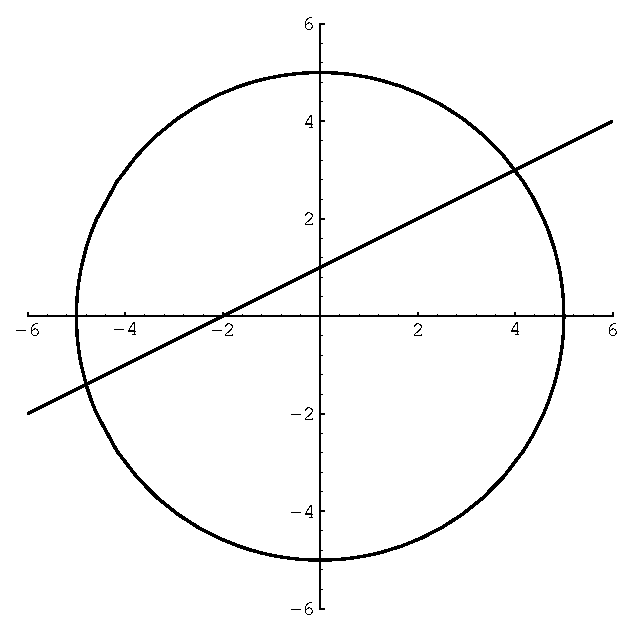
\includegraphics[width=3truein]{CircleLine}
\end{center}
\caption{Simple Algebraic Curves\label{Circle:Fig}}
\end{figure}

Let us start with the simplest type of geometric algebraic object, an
\keyi{algebraic curve}.  By an algebraic curve we mean a one-dimension
set of points whose coordinates satisfy an algebraic equation.  Two
simple examples of algebraic curves are shown in \figref{Circle:Fig},
where we have drawn a circle and straight line.  The points on the
circle are the zeroes of the polynomial $x^2 + y^2 - 25$, while the
line is the zeroes of $3y - x - 2$.  In particular we can define a
plane curve to be the set of zeroes of a polynomial in two variables.

Do the lines in \figref{Circle:Fig} constitute two curves or a single
curves?  It appears that it consists of two separate curves, one
superimposed on the other.  Nonetheless, there is a single polynomial
whose zeroes are the points in \figref{Circle:Fig}.  It is
\[
x^3 - 3 x^2 y + y^2 x - 3 y^3 + 2 x^2 + 2 y^2 - 25 x + 75 y + 50,
\]
which is the product of $x^2 + y^2 - 25$ and $3y - x - 2$.  We
probably want to say that the set of zeroes of an irreducible
polynomial is a single curve (or \keyi{irreducible curve}).

\begin{figure}
\begin{center}
  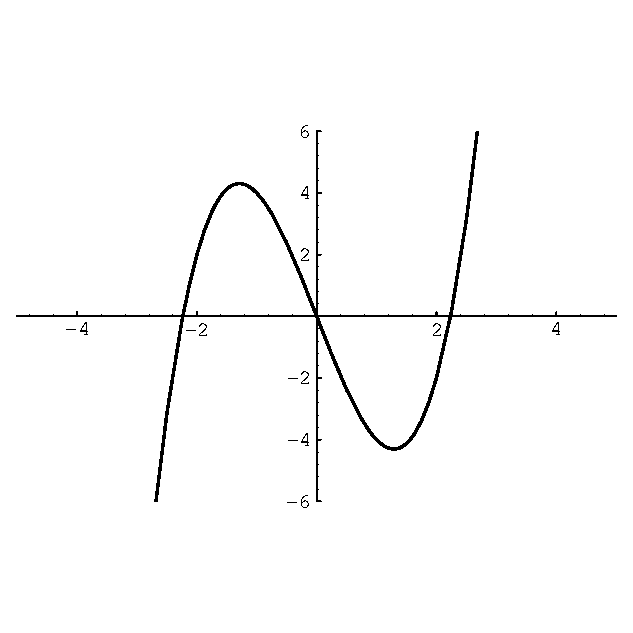
\includegraphics[width=1.5truein]{SimpleCubic1}
    \hfil 
  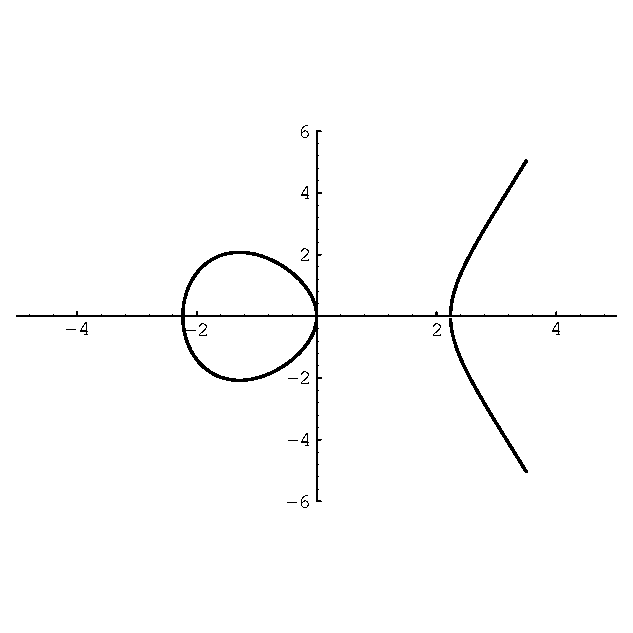
\includegraphics[width=1.5truein]{SimpleCubic2}
\end{center}
\caption{Cubic Curves: $y = x^3 - 5x$ and $y^2 = x^3 - 5x$}
\label{Simple:Cubic:Fig}
\end{figure}

Intuitively we think of the degree of an algebraic curve as the number of
times it can intersect a straight line.  For instance the curves in
\figref{Simple:Cubic:Fig} are obviously of degree three because each
intersects the $x$ axis at three places and no straight line can intersect
them more often.  Similarly the degree of the circle and straight line in
\figref{Circle:Fig} are 2 and 1 respectively.

Notice that a straight line can intersect a sine wave an infinite number of
times.  The sine wave is not an algebraic curve, if it was would have to be the
zeroes of a polynomial of infinite degree.  It is an example of a
transcendental curve.

The second curve of \figref{Simple:Cubic:Fig} is somewhat problematic.
It has two components, but the polynomial $y^2 - x^3 + 5x$ is
irreducible.  One way of looking at this curve is that it is generated
by taking the square roots of the values of $y$ in the
\figref{Simple:Cubic:Fig}(a).  Since there are two values of
$\sqrt{\alpha}$ for each value of $\alpha$, there are two values of
$y$ for each value of $x$ in \figref{Simple:Cubic:Fig}(b).  Notice
that the gap between the loop on the left and the curve on the right
at $x = \sqrt{5}$ arises because the the curve $x^3 - 5x$ is negative
in that region.  Thus the missing values actually lie in the complex
plane.

\begin{figure}
\begin{center}
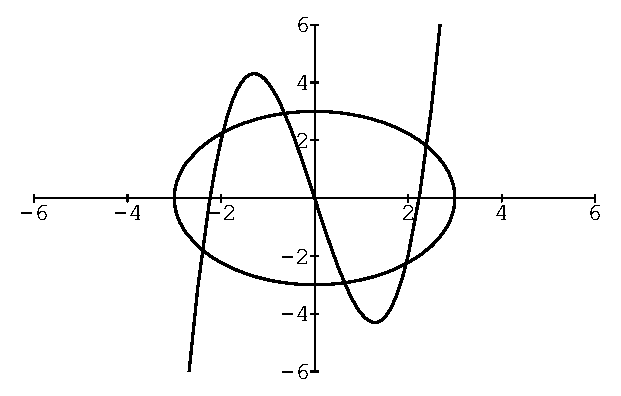
\includegraphics[width=3truein]{SimpIntersection}
\end{center}
\caption{Intersection of a Cubic and a Quadratic\label{Intersect:Fig}}
\end{figure}

Generalizing our observation on the intersection of curves and
straight lines, we would expect that the number of intersections of a
curve of degree $m$ and a curve of degree $n$ would be $mn$.  This is
illustrated by the curves in \figref{Intersect:Fig} where there are
six intersections.  Unfortunately is not always true.  Sometimes there
are fewer intersections.

\begin{figure}
\begin{center}
  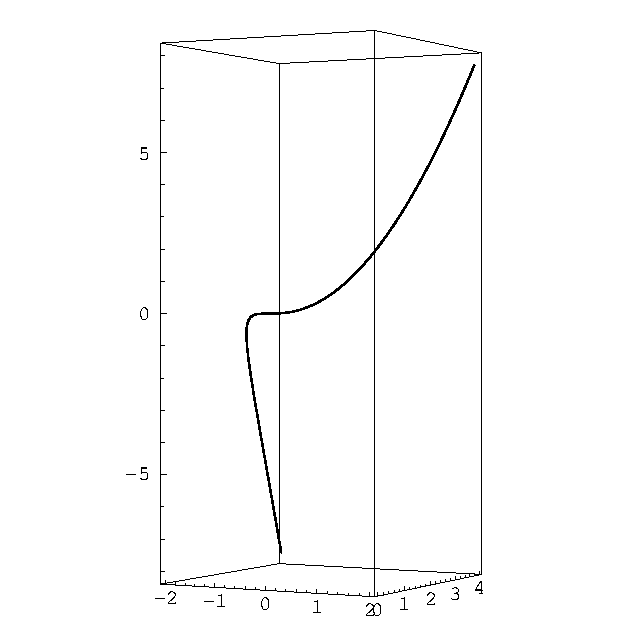
\includegraphics[width=1.5truein]{TwistedCubic1}
    \hfil 
  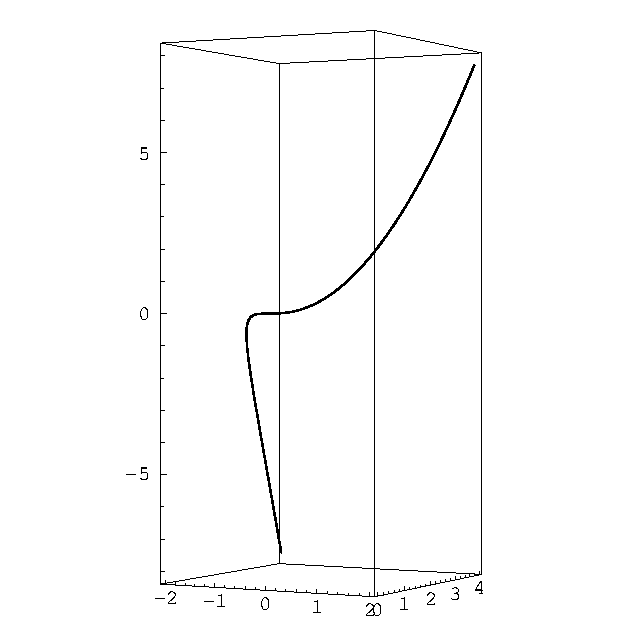
\includegraphics[width=1.5truein]{TwistedCubic2}
\end{center}
\caption{Twisted Cubic\label{Twisted:Cubic:Fig}}
\end{figure}
In three dimensions a single polynomial defines a surface.  In
general the intersection of two surfaces is a curve, although in
exceptional cases it could be a single point or a surface.  An example
of a curve in three dimensions is the \keyi{twisted cubic} shown in
\figref{Twisted:Cubic:Fig}.  This curve is the intersection of the surfaces
\[
y= x^2 \qquad \hbox{and}\qquad z=x^3.
\]
It is a fairly simple example of a curve that cannot be embedded in a
the plane.

\section{Commutative Algebra}

In the most general setting, we begin with a commutative ring $R$.  A
set of elements $I$ is chosen, and used to divide $R$ into equivalence
classes.  Two elements of $R$ are equivalent if their difference is in
$I$.  The set of equivalence classes is denoted by $R/I$.  We will
place restrictions on $I$ so that $R/I$ is still a ring.  For an
element to be equivalent to itself $0$ must be in $I$.  In fact, for
the relationship induced by $I$ to be an equivalence, $I$ must be an
additive group.  It is also not hard to see that if $i$ is an element
of $I$ and $a$ an element of $R$, then $ai$ must be an element of $I$.
Pick two elements of $R$, $r_1$ and $r_2$, such that $r_1 - r_2 = i$.
Since $r_1$ and $r_2$ are equivalent, we must have that $a r_1$ and
$ar_2$ are equivalent.  Thus, $$a r_1 - a r_2 = a \,(r_1 - r_2) = a i
\in I.$$ Sets that have these properties are called ideals.

\begin{definition}
Let $R$ be a commutative ring, and $I$ a subset of $R$.  If $I$ is an
additive group, and if $rI \subset I$ for all $r \in R$, then $I$ is
an \keyb{ideal}.
\end{definition}

\index{ideal, principal} \index{ideal, finitely generated}
In the integer case we used the set of multiples of an integer for
$I$.  The polynomial case described above used multiples of a single
polynomial $p(X)$.  Ideals that are multiples of a single element are
called {\em principal ideals\/}.  We have used the notation $(p)$ to
denote the set of multiples of $p$.  Generalizing this notation
slightly we will let $(a_1, a_2, \ldots, a_n)$ represent the set
\[
S = \{\, a_1 r_1 + a_2 r_2 + \cdots + a_n r_n 
        \mid r_1, r_2, \ldots, r_n \in R \,\}.
\]
$S$ is clearly an ideal. We say that $S$ is {\em generated} by $a_1,
a_2, \ldots, a_n$.  Since $S$ is generated by a finite number of
elements $S$ is called a {\em finitely generated ideal\/}.  There are
rings that have ideals which are not finitely generated, but we will
not discuss them here.  

All rings possess two ideals, the set consisting of the single element $0$
and the whole ring, $R$.  Notice that all the ideals of $R$ contain $(0)$
and are contained in $R$.  The residue class rings of these two ideals are
very dull ($R$ and zero ring) so most of our attention is confined to the
ideals between these two ``trivial'' ideals.

Recall that $\Z/(p)$ had no zero divisors if $p$ was a prime number.  In
fact $\Z/(p)$ is a field in this case.  We will extend
this definition to more general ideals.  Let $R$ be a ring, $I$ an ideal.
$I$ is a {\em prime ideal} if $R/I$ is an integral domain.  If $R/I$ is a
field then $I$ is a {\em maximal ideal\/}.  It is not difficult to see that
these characterizations are equivalent to standard definitions:

\begin{definition}
 $I$ is a \keyi{prime ideal} if for all elements $a$ and $b$
of $R$ such that $ab$ is an element of $I$, either $a$ or $b$ is an
element of $I$.
\end{definition}

\begin{definition}
$I$ is a \keyi{maximal ideal} if there is no ideal $J$ such that $I
\subset J$ other than $R$.
\end{definition}

All maximal ideals are prime.  For $\Z$ all prime ideals  are also maximal.
The situation is not always so simple.  If $R = \Z[X]$ there are three
classes of prime ideals: (p) where $p$ is a prime, $(f(X))$ where $f(X)$ is
an irreducible polynomial, and $(p, f(X))$ where $f(X)$ is irreducible
modulo $p$.  Only the third class leads to a field.

The set of prime ideals of a ring, $R$, is called the ring's
\keyi{spectrum}, $\Spec R$.  It is possible to put a topology on this
space called the \keyi{Zariski topology}.  The point of the space are then the
prime ideals.  Consider the ring $\Z[X]$.  Among the points in the
spectrum are the ideals generated by the linear polynomials $(X - a)$.
Thus there is a clear association between $\Z$ and a subset of the
points in $\Spec \Z$.  Similarly, there is an association between the
elements of $\Z \times \Z$ and the points of $\Spec \Z[X, Y]$.

Let $f$ be an element of $F[X]$, where $F$ is some field.  Let 
$\pger = (X - a)$ be a prime ideal of $F[X]$.  The residue of $f$ modulo
$\pger$ is $f(a)$.  In the spectrum of $F[X]$, the point $\pger$ is
associated with $a$ in $F$.  Thus it is natural to say that $f(a)$ is 
{\em the value of $f$ at $\pger$}.  More generally,
let $f$ be an element of some ring $R$ and $\pger$ a prime ideal of $R$.
The image of $f$ in $R/\pger$ is said to be the value of $f$ at $\pger$ and
is written $f(\pger)$ or $f_{\pger}$.

\medskip

\begin{definition}
A ring is said to be \keyi{Noetherian} if every ideal in the ring is
finitely generated.
\end{definition}

\begin{proposition}
Noetherian rings satisfy the descending chain condition.
\end{proposition}

\index{Hilbert Basis Theorem}
\begin{proposition}[Hilbert Basis Theorem] If $R$ is Noetherian then
$R[X]$ is also Noetherian.
\end{proposition}

\begin{proof}
Let $I$ be an ideal of $R[X]$.  The leading coefficients of the
elements of $I$ form an ideal in $R$ denoted by $\lc(I)$.  Since $R$
is noetherian $\lc(I)$ is finitely generated.  We will use this fact
to construct a basis for $I$.  Let $\{a_1, \ldots, a_n\}$ be a
generating set for $\lc(I)$.  Choose polynomials, $f_1, \ldots, f_n
\in I$ of smallest degree such that the leading coefficient of $f_i$
is $a_i$.  These polynomials generate an ideal $I' \subseteq I$.  Let
the maximum degree of any of the $f_i$ be $r$.  If $\deg f_i < r$,
replace $f$ by $X^{r -\deg f_i} f_i$ so that each of the $f_i$ is of
degree $r$.

We now show that the elements of $I$ are sums of elements of $I'$ and
polynomials of degree less than $r$.  Let $f = a X^m + \cdots$ be a
polynomial in $I$ but not $I'$, and assume $m \ge r$.  Since $\lc(I)$
is finitely generated, we can write $a$ as a linear combination of the
$a_i$
\[
a = c_1 a_1 + \cdots c_n a_n.
\]
The polynomial 
\[
g = X^{m-r} \left[ c_1 f_1 + \cdots c_n f_n \right]
\]
is an element of $I'$ and has the same leading term as $f$.  Repeating
this procedure with $f - g$ we can reduce $f$ to the sum of an element
in $I'$ and an element of $I$ of degree less than $r$.

Now we need to show that the elements of $I$ of degree less than $r$
are finitely generated.  Exactly the same technique is applied.  Let
$J_m$ denote the ideal of the leading coefficients of polynomials in
$I$ of degree $m$ and let $\{ f_{m1}, \ldots, f_{m n_m} \}$ be a set
of polynomials in $I$ of degree $m$ whose leading coefficients
generate $J_m$.  The finite set of polynomials $\{f_i \} \cap \{f_{ij}
\}$ generate $I$.

\end{proof}

The Hilbert Nullstellensatz.  Rabinowitsch's trick in \cite{Rabinowitsch1930-ww}.

\section{Ideal Theoretic Calculations}
\label{Ideal:Arith:Sec}

Given two orders $\ge_{x}$ and $\ge_{y}$ on monomials in $\vec X$ and
$\vec Y$ respectively, we can define an order on $\ge_{xy}$ by $\vec
X^{\vec a} \vec Y^{\vec b} \ge_{xy} \vec X^{\vec a'} \vec Y^{\vec b'}$
if $\vec X^{\vec a} \ge_{x} \vec X^{\vec a'}$ or $\vec X^{\vec a} =
\vec X^{\vec a'}$ and $\vec Y^{\vec b} \ge_{y} \vec Y^{\vec b'}$.

\begin{proposition}[Gianni-Trager-Zacharias]
\label{Lexical:Grobner:Prop}
Let $I$ be an ideal in $R[\vec X, \vec Y]$.  If $G \subset R[\vec X,
\vec Y]$ is a Gr\"obner basis for $I$ with respect to $\ge_{xy}$ then 
\begin{itemize}
\item $G$ is a Gr\"obner basis for $I$ with respect to the order
$\ge_x$ on $(R[\vec Y])[\vec X]$, the polynomial ring with coefficients
in $R[\vec Y]$.
\item $G\cap R[\vec Y]$ is a Gr\"obner basis for $I\cap R[y]$ with
respect to the order $\ge_{y}$.
\end{itemize}
\end{proposition}


\subsection{Ideal Arithmetic}
\label{Ideal:Arithmetic:Sec}

Compute intersection, quotient, dimension, localization of an ideal.

\subsection{Primary Decomposition}

\begin{proposition}[Gianni-Trager-Zacharias]
Let $I$ be a prime zero-dimensional ideal in $k[\vec X]$, 
\[
G = \{g_1(X_1, \ldots, X_n), g_2(X_2, \ldots, X_n), \ldots, g_n(X_n)\}
\]
a minimal Gr\"obner basis for $I$ with respect to $\lexord$.  Then for
almost all linear transformations of coordinates $g_i$ is linear in
$X_i$ for all $i$ less than $n$.
\end{proposition}

\begin{proof}
By the proof of the primitive element theorem, for almost all $a_1,
\ldots, a_n \in k$,
\[
R = k[\vec X]/I \simeq k[a_1 X_1 + \cdots + a_n X_n].
\]
If we choose new coordinates $Z_1, \ldots, Z_n$ such that 
\[
Z_n = a_1 X_1 + \cdots + a_n X_n
\]
then $R = k[Z_n]$.  Since $Z_i \in R$, $Z_i = f_i(Z_n)$ for some
polynomial $f_i$.
\end{proof}

\section{Special Case Lifting Techniques}




%$Id: desingularization.tex,v 1.1 1992/05/10 19:38:30 rz Exp rz $
\chapter{Desingularization}
\label{Desing:Chap}


\section{Puiseux Series}
\label{Puiseux:Sec}

A paper on this is \cite{Cohn1984-zt}.

Original papers by Puiseux \cite{Puiseux1850-rf,Puiseux51}.


%$Id: ratfun-decomp.tex,v 1.1 1992/05/10 19:38:20 rz Exp rz $
\chapter{Rational Function Decomposition}
\label{RatDecomp:Chap}

The problem of determining if a function can be written as the
composition of two ``smaller'' functions $f(x) = g(h(x))$ has been of
interest for a long time.  Although not every function can be
decomposed in this fashion, when such a decomposition does exist many
problems become significantly simpler.  For instance, if $f$ can be
decomposed into equal degree polynomials then its value at different
points can be computed with $O(\sqrt{n})$ multiplications rather than
with $O(n)$ multiplications, as is required in the general case.  In
addition, it is easier to determine if the zeroes of $f$ can be
expressed in terms of radicals if $f$ is decomposable

Until now, work has focused on the univariate, polynomial version of
this problem: When can the polynomial $f(x)$ be written as $g(h(x))$,
where both $g(x)$ and $h(x)$ are polynomials?  The original work in
the symbolic computation community was presented in 1976
\cite{Barton76}, but the algorithms, which in the worst case
required exponential time, were not published until 1985
\cite{Barton85}.  Soon afterward, Kozen and Landau
\cite{Kozen89} provided a polynomial time algorithm for
decomposition of polynomials over fields of characteristic zero that
did not require factorization of polynomials.  Some additional
improvements and an analysis of the positive characteristic case where
then presented by von zur Gathen \cite{Gathen87,Gathen90a}. A number
of other papers have since been published on different extensions and
variations of this problem
\cite{Alagar85,Gutierrez89,Dickerson89a,Dickerson89b}. 

The generalization to rational functions, which has significantly
wider applicability, appears to be a harder problem.  Notice that in
the polynomial case, the degree of $g$ and $h$ must divide the degree
of $f$.  This limits the number of different polynomials that must be
considered and allows one to solve the problem by looking for
solutions of non-linear algebraic equations (admittedly in exponential
time).  When $f$, $g$ and $h$ are rational functions, there is no
immediately obvious bound on the degrees of the numerators of $g$ and
$h$, since the numerator and denominator of $g(h(x))$ could have a
common factor.  In fact, no such common factor can arise, as we prove
below.

Furthermore, we demonstrate that for the rational function problem,
$g$ and $h$ can be determined from $f$ in polynomial time.  This new
algorithm is valid for univariate rational functions with coefficients
in any field over which one can factor polynomials.  Thus this
algorithm can also be used to find polynomial decompositions over
fields of positive characteristic, a problem that was not completely
resolved in earlier work.  Our algorithm requires the factorization of
a polynomial over an algebraic function field---although this can be
done in polynomial time it quite expensive.  Thus our technique is
significantly more costly than the earlier polynomial time algorithms
for the polynomial case, but is far more general.


A number of generalizations of polynomial decomposition are mentioned in
\cite{Barton85}, among which is rational function decomposition.
These generalizations appear to be somewhat {\em ad hoc} and no general
program was presented to guide future work.  This paper discusses a
natural framework, factoring of regular maps between varieties, into which
all previous generalizations of polynomial decomposition can be placed.  In
the one dimensional, univariate case, we develop a lattice of fields that
is in a one to one correspondence with the decomposition of rational
functions.  This result, combined with the subfield determination technique
of Landau and Miller \cite{Landau85b} and a few new ideas,
solves the problem of rational function decomposition over arbitrary fields.
We also present techniques for dealing with some problems from the general
framework.

In \sectref{Applications:Sec} we present two problems that illustrate
where functional decomposition problems arise.  A general frame for
discussion of functional decomposition problems is represented in 
\sectref{Vector:Framework:Sec}.  The mathematical sophistication used
in \sectref{Vector:Framework:Sec} is greater than elsewhere in
this paper, and the results presented there are only used
motivationally in the later sections.  Thus the reader may wish to
skip this section.

\sectref{Generalities:Sec} provides some general background material
about the types of fields that into our discussion of decompositions.
Existence and uniqueness of functional decompositions are
discussed in \sectref{Structural:Results:Sec}.
\sectref{Rational:Function:Decomposition:Sec} presents the new
algorithms for rational function decomposition.  We comment on
previous work and give some conclusions in
\sectref{Conclusions:Sec}.

Two appendices are included to make some fundamental material that is
used in the rational function decomposition algorithm more accessible.
Appendix~\ref{Factoring:Sec} discusses factorization of polynomials
over various rings in a way that we hope makes clearer the
contributions of various investigators.  This appendix was prompted by
an earlier reviewer's comment that factoring polynomials over
algebraic function fields must be harder than factoring over algebraic
number fields.

In Appendix~\ref{Subfield:Sec} we give a new presentation of Susan
Landau's techniques for determining subfields of algebraic extensions.
This work, which allows one to determine properties of the Galois
group of an separable algebraic extension without actually computing
the Galois group appears not to be well understood.  Our short summary
of the techniques and their justification thus seems necessary.



\section{Applications}
\label{Applications:Sec}

The original work on polynomial decomposition algorithms
\cite{Barton85} was motivated by the desire to obtain elementary 
techniques for expressing the zeroes of polynomials in terms of
radicals.  Our starting point was the well known technique for
reducing the degree of palindromic polynomials:
\[
\begin{aligned}
f(x) & = f_0x^{2n} + f_1 x^{2n-1} + \cdots + f_1 x + f_0, \\
     & =  x^n \left( f_0 \left(x + \frac{1}{x}\right)^n 
    + (f_1 - n f_0) \left(x + \frac{1}{x}\right)^{n-1} + \cdots \right), \\
     & = x^n g\left(x + \frac{1}{x}\right). 
\end{aligned}
\]
If $\alpha_1, \ldots, \alpha_n$ are the zeroes of $g(z)$ then the zeroes
of 
\[
x^2 - \alpha_i x + 1 = 0
\]
are the zeroes of $f(x)$.  Furthermore, if the $\alpha_i$ can be expressed
in terms radicals then so can the zeros of $f(x)$.

If $f(x)$ can be decomposed into two polynomials $f(x) =g(h(x))$, then the
zeroes of $f(x)$ are the zeroes of $h(x) = \alpha_i$ where the $\alpha_i$
are the zeroes of $g(x)$.  More generally, let $f(x)$ be decomposed into $f
= g_1 \circ g_2 \circ \cdots \circ g_r$.  If all of the $g_i$ are either
polynomials of degree less than $5$ or of the form $x^m$, then the zeroes
of $f(x)$ can be expressed in terms of radicals.

Within this context the obvious generalization is to the decomposition of
rational functions: When can a rational function be written as the
composition of two rational functions?  However, this doesn't directly
address the problem of solving equations in terms of radicals.  
The decomposition of $f(x)$ in the palindrome case can be written as
\[
f(x) = f_0 (x^2+1)^n + (f_1 - n f_0)(x^2+1)^{n-1} x + \cdots 
\]
So we have written $f(x)$ as $g(x^2+1, x)$, where $g(\cdot, \cdot)$ is
homogeneous and its degreee is half that of $f(x)$.  Thus a more
general question is When do there exist two univariate polynomials $h_1(x)$
and $h_2(x)$ and a homogeneous polynomial $g(x,y)$ such that $f(x) =
g(h_1(x), h_2(x))$?  Partial results have appeared in \cite{Weiss92}.

\medskip
Trager has pointed out another situation where a simple variant of
rational function decomposition naturally occurs.  Assume we wish to
integrate an indefinite integral of the form
\begin{equation}
\label{Integral:Radical:Eq}
\int A(x) \root p \of{B(x)} \, dx,
\end{equation}
where $A(x)$ and $B(x)$ are rational functions in $x$ over some field.
One approach is to determine if there is a rational function $R(x)$,
such that
\[
\int A(x) \root p \of{B(x)} \, dx = \int R(B(x)) \, d\root p \of{B(x)}
  = \int R(y^p) \, dy.
\]
Thus, if such a $R(y)$ can be found, the integral of
\eqnref{Integral:Radical:Eq} can be reduced to the easier problem of
integrating a rational function.  Such an $R(x)$ must satisfy the
functional equation:
\[
R(B(x)) = \frac{p A B}{B'}.
\]
So the integration of \eqnref{Integral:Radical:Eq} is reduced to the
question of when the function $A(x)/B'(x)$ can be written as a
rational function in $B$.

\section{A General Framework}
\label{Vector:Framework:Sec}

Though a number of generalization have been suggested for the
polynomial decomposition problem, they have not been put into a
coherent framework.  One of the main contributions of this paper is to
do just that.

Let $k$ be an {\em arbitrary} field.  The $n$-dimensional {\em affine
space} over $k$, which we denote by $\A^n(k)$, is the set of
$n$-tuples $(a_1, \ldots, a_n)$ where $a_i \in k$.  Two points in
$\A^n(k)$ are equal if and only if their components are equal.  The
$n$-dimensional {\em projective space}, denoted by $\P^n(k)$ is the
set of $n+1$ tuples $(a_0: a_1: \cdots : a_n)$ where the two tuples
$(a_0: a_1: \cdots : a_n)$ and $(b_0: b_1: \cdots : b_n)$ are equal if
there exists a non-zero $r \in k$ such that $r a_i = b_i$ for all $i$.
The colons in the representation indicate that the projective
equivalence relation is to be used.

A {\em regular map} $f: \A^n(k) \rightarrow \A^m(k)$ between two
affine spaces is a map that sends each point $(a_1, \ldots, a_n)$
to the point
\[
(f_1(a_1, \ldots, a_n), \ldots, f_m(a_1, \ldots, a_n)),
\]
where the $f_i$ are polynomials over $k$.  For projective spaces, a
map $f: \P^n(k) \rightarrow \P^m(k)$ is regular if
there are homogeneous polynomials $\{f_0, \ldots, f_m\}$ such that
\[
f : (a_0: a_1: \ldots: a_n) \mapsto 
   (f_0(a_0, \ldots, a_n): \ldots: f_m(a_0, \ldots, a_n)), 
\]
where the $f_i$ have the same total degree.

\begin{figure}
\[
\begin{diagram}
\node{\A^1(k)} \arrow[2]{e,t}{f} \arrow{se,t}{g} \node[2]{\A^1(k)} \\
\node[2]{\A^1{k}}\arrow{ne,t}{h} 
\end{diagram}
\]
\caption{Univariate Polynomial Factorization \label{Polynomial:Factor:Fig}}
\end{figure}

Let $X$ and $Z$ be two spaces (affine or projective) and let
$f:X\rightarrow Z$ be a regular map between them.  We claim that
the correct generalization of the polynomial decomposition problem is:
When does there exist a space $Y$ and regular maps $h:X\rightarrow
Y$ and $g:Y\rightarrow Z$ such that $f$ is equal to $g$ composed
with $h$?  We call this a {\em factorization} of the map $f$.  In this
paper we will be mostly concerned with the situation where $X$, $Y$
and $Z$ are the same spaces (the maps are endomorphisms).  The
simplest cases, endomorphisms of $\A^1(k)$ and $\P^1(k)$, are
precisely the polynomial and rational function decomposition problems.

\subsection{Endomorphisms of $\A^1(x)$ and $\P^1(k)$}
\label{Endo:A1:Sec}

The $X=Y=Z=\A^1(k)$ situation is illustrated in
\figref{Polynomial:Factor:Fig}.  For
$f$ to be regular there must be a univariate polynomial $f_p$ such
that $f$ sends $(x) \in \A^1(k)$ to $(f_p(x))$.  If $f_p(x)$ can be
decomposed into $g_p(h_p(x))$ then regular endomorphisms of $\A^1(k)$,
$g$ and $h$, can be constructed as in \figref{Polynomial:Factor:Fig}.
Conversely assume $f$ factors into $g$ and $h$.  Since all three maps
are regular, there exist corresponding polynomials $f_p$, $g_p$ and
$h_p$.  Since $f(x) = g(h(x))$, $f_p(x) = g_p(h_p(x))$.  

Rational function decomposition corresponds to the case when $X$, $Y$
and $Z$ are $\P^1(k)$, the projective line over some field.  The map
$(x,y) \mapsto (x/y)$ bijectively maps every point in the projective line,
except the ``point at infinity'' $(1, 0)$, to a point of $\A^1(k)$.
We will use this map to convert polynomial statements in projective
space into statements about rational functions.

Since $f$ is a regular endomorphism of $\P^1(k)$ then there exist
homogeneous polynomials $f_1$ and $f_2$ such that
\[
f : (x: y) \mapsto (f_1(x, y) : f_2(x, y)).
\]
For every point of $\P^1(k)$, except $(1 : 0)$, this map is equivalent to
the rational function
\[
f_r(z) = \frac{f_1(z, 1)}{f_2(z, 1)}
\]
where $(x : y) \mapsto (f_r(x/y) : 1)$.  Although $f_1(x, y)$ and
$f_2(x, y)$ have the same total degree, observe that $f_1(z, 1)$ and
$f_2(z, 1)$ need not have the same degree.  A rational function
\[
f_r(z) = \frac{p(z)}{q(z)} 
= \frac{p_{0} z^m + p_{1} z^{m-1} + \cdots + p_{m}}{q_0 z^n + q_1
z^{n-1} + \cdots + q_n}
\]
induces a regular endomorphism of $\P^1(k)$ as follows.  For
simplicity, assume $m > n$.  The point $(x, y) \mapsto (f_1(x, y),
f_2(x, y))$ where
\[
\begin{aligned}
f_1(x, y) &= y^m p\left(\frac{x}{y}\right) = p_0 x^m + p_1 x^{m-1} y +
\cdots + p_m y^m \\
f_2(x, y) &= y^m q\left(\frac{x}{y}\right) = q_0 x^n y^{m-n} + q_1 x^{n-1} y^{m-n+1} +
\cdots + q_m y^n 
\end{aligned}
\]

Now assume there are regular endomorphisms $g$ and $h$ (with similar
components) such that $f = g \circ h$.  Composing the maps, we have
\[
\begin{aligned}
f_1(x, y) & = g_1(h_1(x,y), h_2(x,y)), \\
f_2(x, y) & = g_2(h_1(x,y), h_2(x,y)).
\end{aligned}
\]
Formally write the quotient of these two equations:
\[
\begin{aligned}
\frac{f_1(x, y)}{f_2(x, y)} 
    & = \frac{g_1(h_1(x,y), h_2(x,y))}{g_2(h_1(x,y), h_2(x,y))}, \\
    & = \frac{g_1(\frac{h_1(x,y)}{h_2(x,y)},1)}{g_2(\frac{h_1(x,y)}{h_2(x,y)}, 1)},
\end{aligned}
\]
where the division by $h_2(x, y)$ is valid because $g_1$ and $g_2$
have the same total degree.  Or, writing $z = x/y$
\[
f_r(z) = \frac{f_1(z,1)}{f_2(z,1)} 
 = \frac{g_1(\frac{h_1(z,1)}{h_2(z,1)},1)}{g_2(\frac{h_1(z,1)}{h_2(z,1)}, 1)}
 = g_r(h_r(z)).
\]
Thus the factorization of an endomorphism of a projective line
generated by a rational function is equivalent to decomposition of the
rational function.

In this framework, the decomposition problems discussed in
\cite{Barton85,Alagar85,Gutierrez89,Gathen87} are equivalent to the
factorization of endomorphisms of $\A^1(\Q)$.  Kozen and Landau
\cite{Kozen89} and von zur Gathen \cite{Gathen90a,Gathen90b} consider
the morphism factorization problem for $\A^1(\F_q)$, but do not
provide polynomial time algorithms in all cases.  The multivariate
decomposition problem solved by Dickerson \cite{Dickerson89b} deals with endomorphisms of $\A^1(k[\vec x])$.

In this paper we give a polynomial time reduction of the endomorphism
factorization problem over $\P^1(k)$ to factorization of polynomials
over $k$.  As a special case this also resolves the problem for
$\A^1(k)$.

\subsection{Endomorphisms of $\A^n(k)$ and $\P^n(k)$}
\label{Endomorphism:An:Sec}

Within the framework of factoring regular maps, the natural
``multivariate'' generalization to consider is factorization of
endomorphisms of affine and projective spaces of higher dimension.
For instance, let $f$ be a regular endomorphism of the affine plane
$\A^2(k)$ and let $(a_1, a_2)$ be an element of $\A^2(k)$.
Then there are a pair of polynomials $f_1, f_2 \in k[x,y]$ such that 
\[
f(a_1, a_2) = (f_1(a_1, a_2), f_2(a_1, a_2)).
\]
If $f$ factors into two maps $g$ and $h$, $f = g \circ h$, then the
polynomial components of $g$ and $h$ satisfy:
\begin{equation}\label{2D:Affine:Decomp:Eq}
\begin{aligned}
f_1(x, y) & = g_1(h_1(x, y), h_2(x, y)), \\
f_2(x, y) & = g_2(h_1(x, y), h_2(x, y)).
\end{aligned}
\end{equation}

A regular endomorphism of $\P^2(k)$ is a triple of co-prime homogeneous
polynomials
\[
(f_1(x,y,z): f_2(x,y,z): f_3(x,y,z)).
\]
If $g$ and $h$ are also regular endomorphisms such that $f = g \circ
h$ then 
\[
(f_1 : f_2 : f_3) =
 (g_1(h_1, h_2, h_3) : g_2(h_1,h_2,h_3) : g_3(h_1, h_2, h_3)).
\]
Since $(x:y:z) \in \P^2(k)$ and the polynomials are homogeneous, we can
rewrite this as
\[
\begin{aligned}
  \frac{f_1(x,y,1)}{f_3(x,y,1)} & 
   = \frac{g_1(\frac{h_1(x,y,1)}{h_3(x,y,1)},\frac{h_2(x,y,1)}{h_3(x,y,1)},1)}
          {g_3(\frac{h_1(x,y,1)}{h_3(x,y,1)},\frac{h_2(x,y,1)}{h_3(x,y,1)},1)},\\
  \frac{f_2(x,y,1)}{f_3(x,y,1)} & 
   = \frac{g_2(\frac{h_1(x,y,1)}{h_3(x,y,1)},\frac{h_2(x,y,1)}{h_3(x,y,1)},1)}
          {g_3(\frac{h_1(x,y,1)}{h_3(x,y,1)},\frac{h_2(x,y,1)}{h_3(x,y,1)},1)}.
\end{aligned}
\]
Identifying the rational functions $F_i(x,y)$ with $f_i/f_3$ and
similarly for $G_i$ and $H_i$ we have
\begin{equation}\label{2D:Projective:Decomp:Eq}
\begin{aligned}
F_1(x, y) & = G_1(H_1(x, y), H_2(x, y)), \\
F_2(x, y) & = G_2(H_1(x, y), H_2(x, y)).
\end{aligned}
\end{equation}
Comparing \eqnref{2D:Affine:Decomp:Eq} with
\eqnref{2D:Projective:Decomp:Eq} we see that passing from
endomorphisms of $\A^2(k)$ to endomorphims of $\P^2(k)$ converts the
bivariate polynomial decomposition problem to the corresponding
rational function decomposition problem.  These higher dimensional
endomorphism problems are much harder than the one dimensional problem
of \sectref{Endo:A1:Sec}.


\subsection{Endomorphisms of Curves}
\label{Endo:Curves:Sec}

In addition to dealing with endomorphism of $\A^n$ and $\P^n$ we can
discuss endomorphisms of other algebraic structures, like algebraic
curves.  Perhaps the most interesting class of curves from this
perspective are elliptic curves such as
\[
E: y^2 = x^3 - x,
\]
which in projective space has a huge number of endomorphisms.  For
instance, 
\[
(x:y:z) \mapsto (2(x^2+z^2)^2 : x^6-5x^4 z^2 - 5 x^2 z^4 + z^6 :
  (8x^3 - 8 x)y).
\]
For simplicity, we write these maps as rational functions, allowing us to
drop the third coordinate.  The previous endomorphism is then
\begin{equation} \label{Double:Endo:Eq}
(x, y) \mapsto \left( \frac{x^4+2x^2+1}{4x^3-4x}, 
  \frac{x^6-5x^4-5x^2+1}{8(x^3-x)^2}y\right).
\end{equation}
All endomorphisms of elliptic curves are of the form $(p(x), q(x)
y)$, where $p(x)$ and $q(x)$ are rational functions.  

Points on an elliptic curve obey a group law
\cite{SilvermanJH86}.  If $P_i = (x_i, y_i)$ are points on
the elliptic curve $E_{a,b} : y^2 = x^3+ax+b$ then $P_3 = P_1 + P_2$
when
\[
\lambda = \left\{\begin{array}{ll}
  \displaystyle\frac{y_2 - y_1}{x_2 - x_1} & \mbox{if $P_1 \not= P_2$}\\
  \displaystyle\frac{3x_1^2+a}{2y_1} & \mbox{if $P_1 = P_2$}
 \end{array}\right.
\]
and
\[
\begin{aligned}
  x_3 & = - (x_1 + x_2) + \lambda^2, \\ 
  y_3 & = -y_1 - \lambda (x_3 - x_1).
\end{aligned}
\]
The endomorphism \eqnref{Double:Endo:Eq} sends
$P_1\mapsto P_1 + P_1 = 2P_1$, which is denoted by $[2]$.  Similarly,
we can generate endomorphisms corresponding to multiplication by any
positive number $[n]$.  The additive inverse of $P_1 = (x_1, y_1)$ is
$(x_1, - y_1)$, so we have 
\[
[-1] : (x, y) \mapsto (x, - y),
\]
and thus we have an endomorphism of $E_{a,b}$ for each element of
$\Z$.

In addition there are occasionally additional endomorphims.  For
instance, the map 
\[
[i] : (x, y) \mapsto (-x, iy)
\]
is an endomorphism of $y^2 = x^3 -x$.  Clearly, $[i] \circ [i] =
[-1]$.  Using the additional formula given above, we can compute the
endomorphism $[1+i]$:
\[
[1+i] : (x, y) \mapsto \left(-\frac{i}{2}\left(x - \frac{1}{x}\right),
  -\frac{1+i}{4}\left(1 + \frac{1}{x^2}\right) y\right).
\]
Composing $[1+i]$ with itself we have
\[
\begin{aligned}
\relax [1+i]\circ[1+i](x,y) & = \left(
-\frac{x^4+2x^2+1}{4x^3-4x}, \frac{i(x^6-5x^4-5x^2+1)}{8(x^3-x)^2}y\right)\\
& = [i] \circ [2] (x,y).
\end{aligned}
\]
In fact there is an isomorphism between $\End(E_{-1,0})$ and $\Z[i]$.

\section{Preliminaries}
\label{Generalities:Sec}

\subsection{Geometry}
The geometric formulation of the decomposition problem leads very
naturally discussed in \sectref{Vector:Framework:Sec} lead very
naturally to the algebraic problems that are resolved in the body of
this paper. 

Let $X$ be an affine variety embedded in $\A^n(k)$.  Recall that the
ideal of $X$ is $I(X) \subseteq k[x_1, \ldots, x_n]$, the set of all
polynomials that vanish on $X$.  The {\em coordinate ring} of $X$,
$\Gamma(X)$, is defined to be $k[x_1, \ldots, x_n]/I(X)$.  The
elements of the coordinate ring can be identified with the polynomial
functions from $X$ to $k$.  Notice that when $X = \A^1(k)$, $\Gamma(X)
= k[x_1]$.  The quotient field of the coordinate ring $\Gamma(X)$ is
called the {\em function field} of $X$ and is denoted by $K(X)$.  For
$X=\A^1(k)$, $K(X) = k(x_1)$.

A polynomial map $f: X \rightarrow Z$ induces a homomorphism between
between coordinate rings, $f^{\ast}: \Gamma(Z) \rightarrow
\Gamma(X)$, as follows.  Let $p$ be an element of $\Gamma(Z)$, then $p$ is a
polynomial from $Z$ to $k$.  $f^{\ast}(p)$ is the polynomial map from
$X$ to $k$ defined by $f^{\ast}(p) = p \circ f$.  This homomorphism
can be canonically extended to one between function fields:
$f^{\ast}:K(Z) \rightarrow K(Z)$.  When $X$ and $Z$ are
irreducible, have the same dimension and $f(X)$ is dense in $Z$ then
$K(X)$ is an algebraic extension of $f^{\ast} K(Z)$.  ($\A^n(k)$ and
$\P^n(k)$ are irreducible and both have dimension $n$.)

\begin{figure}
\[
\begin{diagram}
\node{X} \arrow[2]{e,t}{f} \arrow{se,t}{g} \node[2]{Z} \\
\node[2]{Y}\arrow{ne,t}{h} 
\end{diagram}
\]
\caption{Morphism Factorization \label{Morphism:Factorization:Fig}}
\end{figure}

For example let $X = Z = \A^1(k)$ and let $f : X \rightarrow Z$ be
a map such that $(a_1) \mapsto (a_1^2) \in Z$.  The coordinate rings
of $X$ and $Z$ are both $k[x] = \Gamma(X) = \Gamma(Z)$.  Let $p(x) =
x^3+x$ be an element of $\Gamma(Z)$, then $f^{\ast}(p) = p \circ f =
x^6+x^2$. Furthermore, $f^{\ast}(\Gamma(Z)) = k[x^2] \subseteq
\Gamma(X)$.  Passing to the function fields, we see that $f^{\ast}K(Z)
= k(x^2)$ and $K(X) = k(x)$.

The relationship between $f^{\ast}K(Z)$ and $K(X)$ is the key to
understanding the behavior of morphism under composition and thus
generalizations of the polynomial decomposition problem.  Consider, for
instance, a factorization of $F$ as indicated in
\figref{Morphism:Factorization:Fig}.  The previous discussion shows
that both $h^{\ast}K(Y)$ and $f^{\ast}K(Z)$ are subfields of $K(X)$
and that $g^{\ast}K(Z)$ is a subfield of $K(Y)$.  This gives the
field structure indicated in \figref{Variety:Structures:Fig}.

\begin{figure}
\[
\begin{diagram}
\node{K(X)} \arrow{s,,-} \\
\node{h^{\ast}K(Y)} \arrow{e,t}{k^{\ast}} \arrow{s,,-} \node{K(Y)} \arrow{s,,-}\\
\node{f^{\ast}K(Z)} \arrow{e,t}{h^{\ast}} \node{g^{\ast} K(Y)}
\end{diagram}
\]
\caption{Fields involved in decomposition \label{Variety:Structures:Fig}}
\end{figure}

A finite morphism $f:X \rightarrow Z$ has a non-trivial
factorization if and only if there is an intermediate field between
$K(X)$ and $f^{\ast}K(Z)$.  Once such an intermediate field is found,
it is still necessary to reconstruct $g$, $h$ and $Y$ from it.  This
can be quite difficult.

\subsection{Field Structure}
We need to use fields that have a rather unusual presentation,
$k(f(x))$ where $f(x)$ is a rational function.  For example, the field
$k(x^2)$ is the field of rational functions in $x^2$, \eg,
\[
\frac{x^4 + x^2 + 1}{x^4 + 1} \in k(x^2),
\]
but $x$ and $x^2 + x$ are not elements of $k(x^2)$.  There is an
isomorphism between $k(x^2)$ and $k(t)$, with $x^2 \mapsto t$.
At the same time, however, $k(x^2)$ can be embedded in $k(x)$ by $x^2
\mapsto x^2$.  Since $k(x^2)$ and $k(x)$ both have transcendence
degree $1$ over $k$ and $k(x^2) \varsubsetneq k(x)$, $k(x)$
must be an algebraic extension of $k(x^2) = k(t)$.  In fact, $x =
\sqrt{t} =\sqrt{(x^2)}$, so the algebraic degree of $k(x)$ over
$k(x^2)$ is $2$.  The following diagram illustrates this.
\[
\begin{diagram}
\node{k(x)} \arrow{s,,-}\arrow{e,t,-}{\cong}
  \node{E[\alpha]/(\alpha^2-t)} \arrow{s,,-} \\
\node{k(x^2)} \arrow{e,t,-}{\cong} \node{E=k(t)}
\end{diagram}
\]
Each of the horizontal lines are isomorphisms.  At the bottom we have
$x^2 \mapsto t$, while the top line is $x \mapsto \alpha$.

Let $p(x)$ be a polynomial over $k$ and denote by $k(p(x))$ the field
of rational functions in $p(x)$.  Using the same notation as the in
the diagram above, the minimal polynomial for $\alpha$, which
generates $k(x)$ over $k(p(x))$, is $p(\alpha) -
t$.  Since this polynomial is linear in $t$, it is irreducible and
the degree of the polynomial $p$ is the algebraic degree of $k(x)$
over $k(p(x))$.

More generally, if $f(x)$ is a rational function over $k$, $k(f(x))$
is the field of rational functions in $f(x)$.  We extend the notion of
degree of a polynomial by defining the {\em degree} of a rational
function $f(x)$, also denoted 
by $\deg f$, to be the maximum of the polynomial degrees of the
(relatively prime) numerator and denominator of $f$.  For polynomials,
the degree of the field $k(x)$ over $k(f(x))$ was shown to be the
degree of $f$.  This is also true for rational function, as shown by
the following proposition.

\begin{proposition}
\label{Luroth:Extension:Degree:Prop}
Let $k(x)$ be an extension of the field $k(f(x))$ where $f(x)$ is a
rational function of degree $n$.  Then $\fieldDegree{k(x)}{k(f(x))} = n$.
\end{proposition}

\begin{proof}
Denote the numerator of $f(x)$ by $p(x)$ and the denominator by
$q(x)$.  Without loss of generality we can assume that $p$ and $q$ are
relatively prime.
We can consider instead the isomorphic fields $k(t) \cong
k(f(x))$ as the ground field, and
\[
k(t)[x]/(p(x) - t q(x)) \cong k(x)
\]
as an algebraic extension of $k(t)$.  $P(x,t) = p(x) -t q(x)$ is primitive
as a polynomial in $t$ since $p(x)$ and $q(x)$ are relatively prime.  Since
it is linear in $t$ it is irreducible.  Therefore, the degree of $x$ over
the field $k(t)$ is
\[
\deg_{x} P(x,t) = \max( \deg p, \deg q) = \deg f.
\]
\end{proof}

\noindent
Notice that $k(x)$ is integral over $k(f(x))$ if and only if $f(x)$ is
a polynomial.

An extremely important tool in this study is the following proposition
on the degree of the composition of two rational functions.  It is
clear for polynomials that the degree of $g\circ h$ is the product of
$\deg g$ and $\deg h$.  The following proposition shows that this is
also true for rational functions.  This proposition is well known in
mathematical circles.  See the comment after definition 1 in
\cite{Fried74}. 

\begin{figure}
\[
\begin{diagram}
\node{k(x)} \arrow{s,,-} \\
\node{k(h(x))} \arrow{e,t}{\varphi_h} \arrow{s,,-} \node{k(y)} \arrow{s,,-}\\
\node{k(f(x))} \arrow{e,t}{\varphi_h} \node{k(g(y))}
\end{diagram}
\]
\caption{Fields involved in decomposition \label{Bound:Field:Fig}}
\end{figure}

\begin{proposition}
\label{RatDecomp:Bound:Prop}  Let $k$ be an arbitrary field, and 
assume $f(x)$, $g(x)$ and $h(x)$ are elements of $k(x)$ such that
$f(x) = g(h(x))$.  Then
\[
\deg f = (\deg g) \cdot (\deg h)
\]
\end{proposition}

\begin{proof}
Consider the fields shown in \figref{Bound:Field:Fig}.  The map
$\varphi_h : y \mapsto h(x)$ is an isomorphism of $k(y)$ onto
$k(h(x))$ and restricted to $k(g(y))$ it yields an isomorphism of
$k(g(y))$ onto $k(f(x))$.

By \propref{Luroth:Extension:Degree:Prop}, the degree of each of
the extensions is
\[
\begin{aligned}
\fieldDegree{k(x)}{k(h(x))} & = \deg h, \\
\fieldDegree{k(x)}{k(f(x))} & = \deg f, \\
\fieldDegree{k(y)}{k(g(y))} & = \deg g. 
\end{aligned}
\]
$k(h(x))$ is an algebraic extension of $k(f(x))$ inside $k(x)$.  Thus,
\[
\begin{aligned}
  \deg f = \fieldDegree{k(x)}{k(f(x))} & = \fieldDegree{k(x)}{k(h(x))}
      \cdot \fieldDegree{k(h(x))}{k(f(x))} \\
    & =\fieldDegree{k(x)}{k(h(x))} \cdot \fieldDegree{k(y)}{k(g(y))} 
      = (\deg h) \cdot (\deg g).
\end{aligned}
\]
\end{proof}

\medskip
The lattice structure of fields of the form $k(f(x))$ is central to
our study of functional decomposition.  There are four basic questions
whose resolution would clarify this lattice structure:
\begin{itemize}
\item[{\bf A}] When is $k(f_1(x)) \subseteq k(f_2(x))$?
\item[{\bf B}] When is $k(f_1(x))$ equal to $k(f_2(x))$?
\item[{\bf C}] Can we explicitly represent $k(f_1(x), f_2(x))$, the smallest
field containing $k(f_1(x)) \cup k(f_2(x))$?
\item[{\bf D}] Can we explicitly represent $k(f_1(x)) \cap k(f_2(x))$?
\end{itemize}
Questions {\bf A} and {\bf B} are relatively easy and are answered
below.  Question {\bf C} is not difficult, but our solution requires
L\"uroth's theorem and is discussed a bit later.  The final question
seems somewhat difficult.  We do not have a complete answer at this
time.

We begin with the first question.  If there exists a rational function
$g(x)$ with coefficients in $k$ such that $f_1(x) = g(f_2(x))$, then
$f_1(x)$ will be an element of $k(f_2(x))$ and each element of
$k(f_1(x))$ will be an element of $k(f_2(x))$.  Conversely, if
$f_1(x)$ is in $k(f_2(x))$ then there must exist a rational function
$g(x)$ such that $f_1(x) = g(f_2(x))$.  Thus we have the following
proposition, which also appears in Weber \cite{Weber:Algebra:II},
\S$126$.

\begin{proposition} \label{Luroth:Subfield:Prop}
$k(f_1(x)) \subseteq k(f_2(x))$ if and only if there exists a rational
function $g(x) \in k(x)$ such that $f_1(x) = g(f_2(x))$.
\end{proposition}

If two fields $k(f_1(x))$ and $k(f_2(x))$ are equal then by the
\propref{Luroth:Subfield:Prop}, there exist rational functions $\lambda_1(x)$ and
$\lambda_2(x)$ such that
\[
\begin{aligned}
f_1(x) & = \lambda_1(f_2(x))\quad \mbox{and}\\
f_2(x) & = \lambda_2(f_1(x)),
\end{aligned}
\]
which means that
\[
f_1(x) = \lambda_1(\lambda_2(f_1(x)))
\]
or $\lambda_1(\lambda_2(x)) = x$.  Applying
\propref{RatDecomp:Bound:Prop} we see that 
\[
(\deg \lambda_1) \cdot (\deg \lambda_2) = 1.
\]
Since the degree of a rational function is a non-negative integer, the
only rational functions that can have inverse are those that are the
ratio of two linear polynomials.  

Such a rational function is called a {\em fractional linear} function:
\[
\lambda(x) = \frac{a x + b}{c x + d}.
\]
If either $cx+d$ divides $ax+b$ or $a=c=0$ then the degree of
$\lambda(x)$ will be $0$.  Such fractional linear function is called
{\em degenerate\/}.  In the first case,
\[
\frac{a}{c} = \frac{b}{d},
\]
or $ad - bc = 0$.  In the second case, $a=c=0$, $ad -bc$ is also zero.
Thus a necessary a sufficient condition for $\lambda(x)$ to have
degree $1$ is that $ad-bc \not=0$.  

If a fractional linear function is not degenerate then its inverse
under composition is
\[
\lambda^{-1}(x) = \frac{-dx + b}{cx - a}.
\]
Thus we have the following proposition, which answers our second
fundamental question.

\begin{proposition}\label{Bilinear:Inverse:Prop}
If $k(x)$ is equal to $k(y)$ then there exists a fractional linear
function $\lambda$ with coefficients in $k$ such that $x =
\lambda(y)$.  In particular, if $k(f_1(x))$ is equal to $k(f_2(x))$
then there exists a bilinear function $\lambda$ such that $f_1(x) =
\lambda(f_2(x))$ and $f_2(x) = \lambda^{-1}(f_1(x))$.
\end{proposition}

If $f(x) = g(h(x))$ then \propref{RatDecomp:Bound:Prop} provides
bounds on the degrees of $g(x)$ and $h(x)$ in terms of the degree of
$f(x)$.  Thus in principal we have an algorithm for rational function
decomposition: Set up a system of algebraic equations in the
undetermined coefficients of $g$ and $h$.  Any solution to the system
in $k$ will yield a decomposition of $f(x)$.  This algorithm is
exponential time.  In \sectref{Rational:Function:Decomposition:Sec} we
present efficient algorithms.

\medskip
The link between field structure and rational function decomposition
comes from {\em L\"uroth's theorem\/}, which was proven by L\"uroth
\cite{Luroth76} for $k = \C$ and by Steinitz in general
\cite{Steinitz10}.

\begin{proposition}[L\"uroth]
\label{Luroths:Prop}
If $k \varsubsetneq K \subset k(x)$ then $K = k(g(x))$ where $g(x)$ is
a rational function in $x$.
\end{proposition}

\noindent
An elementary proof of L\"uroth's theorem may be found in van der
Waerden \cite{Waerden:Algebra}.  An effective proof appears in
Weber \cite{Weber:Algebra:II} \S$124$, and in English in Schinzel
\cite{Schinzel:Polynomials}.

L\"uroth's theorem says that each field in the lattice of subfields
between $k(x)$ and $k$ that has transcendence degree $1$ over $k$
is generated by a single rational function.  In particular, $k(f_1(x),
f_2(x)) = k(h(x))$ for some rational function $h(x)$ and either
$k(f_1(x)) \cap k(f_2(x)) = k(g(x))$ for some rational function $g(x)$
or their intersection is $k$.  We will show, for instance that
$k(x^2+1)\cap k(x^3+1) = k$ in \sectref{Decomposition:Uniqueness:Sec}. 

Using L\"uroth's theorem question {\bf C} can be addressed
straightforwardly.  We have the following sequence of fields:
\[
k(x) \supseteq k(f_1(x), f_2(x)) \supseteq k(f_1(x)),
\]
where both $k(x)$ and $k(f_1(x), f_2(x))$ are algebraic extensions of
$k(f_1(x))$.  In particular $x \in k(x)$ is algebraic over
$k(f_1(x))$.  To make this more explicit we write $k(f_1(x)) = k(t)$
and
\[
k(x) = k(t)[\alpha]/(p(\alpha)),
\]
where $p(\alpha)$ is the minimal polynomial of $x$ over $k(f_1(x))$,
\ie,
\[
p(Z) = \num (f_1(Z) - t) = \num f_1(Z) - t \den f_2(Z).
\]
In terms of $\alpha$, $k(f_1(x), f_2(x)) = k(t)[f_2(\alpha)]$.  
$f_2(\alpha)$ is a zero of the polynomial
\[
\prod_{f_1(\alpha_i) = 0} \left(Z - f_2(\alpha_i)\right) = q(t, Z),
\]
where the product is over the zeroes of $f_1(Z)$.  The coefficients of
$q(t, Z)$ lie in $k$.  It can be computed using resultants as
\[
q(t, Z) = \Norm_{k(x)/k(f_1(x))} Z - f_2(\alpha) 
        = \res_u (f_1(u), Z- f_2(u)).
\]
By \propref{Sqfr:Norm:Prop}, $q(t, Z)$ is the power of an irreducible
polynomials, which we denote by by $Q(t, Z)$.  $Q(t, Z)$ can be
computed by taking the GCD of $q(t, Z)$ and $q_Z(t,Z)$ or explicitly
computing the $r$\th{} roots of $q(t,Z)$, where $r$ divides the degree
of $q(t,Z)$.nn

Any zero of $q(t, Z)$ (or $Q(t,Z)$) generates $k(f_1(x), f_2(x)) =
k(h(x))$.  Further, by L\"uroth's theorem such a zero must be a
rational function in $x$.  Thus $Z - h(x)$ must divide $q(f_1(x), Z)$.
So $h(x)$ can be obtained by examining a linear factor of the
$q(f_1(x), Z)$.

\subsection{Normal Subfields of $k(x)$}
\label{Normal:Subfields:Sec}

If $E$ is a subfield of $k(x)$, then we call it a {\em normal
subfield} if $k(x)/E$ is a normal extension.  By L\"uroth's theorem we
know that all subfields of $k(x)$ are of the form $k(g(x))$ for some
$g(x)$, or $k$.  It is also interesting to find out which of those subfields
are normal subfields.  As we shall see, if $k(x)/k(g(x))$ is normal
then $g(x)$ has some very interesting properties.

Since $k(x)/k$ is not an algebraic extension, the only normal
subfields are finite degree subfields of $k(x)$.  By
\propref{Bilinear:Inverse:Prop} the only automorphisms of $k(x)$ are
those that send
\[
x \mapsto \frac{ax+b}{cx+d}.
\]
The set of such automorphisms is isomorphic to the group
$\mbox{SL}_2(k)/\{\pm I\}$ of $2\times 2$ matrices with determinant
equal to $1$.  If $k(x)$ is normal over $E$, then the Galois group of
$k(x)/E$ must be a finite subgroup of $\mbox{SL}_2(k)/\{\pm I\}$.
Thus the problem of determining all normal subfields of $k(x)$ is
equivalent to finding all normal subgroups of $\mbox{SL}_2(k)/\{\pm
I\}$.

The study of the finite subgroups of $\mbox{SL}_2(\C)/\{\pm I \}$ has
a long history.  Any finite subgroup corresponds to a rotation or
reflection of the Riemann sphere, so the finite subgroups correspond
to the regular solids in three dimensions and date back to the Greeks.

Klein \cite{Klein75} gave the first modern, geometric proof that there
were only finitely many subgroups of $\mbox{SL}_2(\C)/\{\pm I\}$.  In
the context of monodromy groups of differential equations, Jordan
\cite{Jordan76} gave a proof using Sylow groups.  He extended
this work to the finite subgroups of $\mbox{SL}_2(\C)/\{\pm I\}$ in
\cite{Jordan:1878}.  Gordan \cite{Gordan77} considered these groups
from the perspective of invariant theory.  A good discussion is in
\cite{Klein56}.

\begin{proposition}[Klein] \label{Klein:Groups:Prop}
The finite subgroups of $\mbox{SL}_2(\C)/\{\pm I \}$ are of one of the
following five types:
\begin{itemize}
\item $C_n$, the cyclic group of order $n$;
\item $D_n$, the dihedral group of order $n$;
\item $A_4$, the alternating group on four letters or tetrahedral group;
\item $S_4$, the symmetric group on four letters or octahedral group;
\item $A_5$, the alternating group on five letters or icosahedral group.
\end{itemize}
\end{proposition}

The elements of these groups, as subgroups of $\mbox{SL}_2(k)/\{\pm I\}$ are as
follows.  The elements of the cyclic group are:
\[
C_n = \left\{\zeta_n z \right\}.
\]

For the dihedral group, the elements are:
\[
D_n = \left\{ \zeta_n z, \frac{1}{\zeta_n z} \right\}
\]

For the tetrahedral group:
\[
\left\{
 \pm z, \pm \frac{i}{z}, 
 \pm \frac{(1+i)z + \sqrt{2}}{\sqrt{2}z - 1 + i},
 \pm \frac{\sqrt{2}z - 1 + i}{(1+i)z + \sqrt{2}},
 \pm \frac{(1-i)z + \sqrt{2}}{\sqrt{2}z - 1 - i},
 \pm \frac{\sqrt{2}z - 1 - i}{(1-i)z + \sqrt{2}}
\right\}
\]

The octahedral group has two different representations:
\[
\left\{
 i^k z, \frac{i^k}{z}, 
 i^k\frac{z+1}{z-1}, i^k\frac{z-1}{z+1}, 
i^k\frac{z+i}{z-i}, i^k\frac{z-i}{z+i}
\right\}
\]
and
\[
\left\{
  i^k z, \frac{i^k}{z}, 
 i^k \frac{(1+i)z + \sqrt{2}}{\sqrt{2}z - 1 + i},
 i^k \frac{\sqrt{2}z - 1 + i}{(1+i)z + \sqrt{2}},
 i^k \frac{(1-i)z + \sqrt{2}}{\sqrt{2}z - 1 - i},
 i^k \frac{\sqrt{2}z - 1 - i}{(1-i)z + \sqrt{2}}
\right\}
\]
where $k = 0, 1, 2, 3$.

And for the icosahedral group:
\[
\left\{
  \zeta_5^{\mu} z, - \frac{1}{\zeta_5^{\mu} z},
  \zeta_5^{\nu} 
   \frac{-(\zeta_5-\zeta_5^4)\zeta_5^\mu z + \zeta_5^2-z\zeta_5^3}
        {(\zeta_5^2-\zeta_5^3)\zeta_5^\mu z + \zeta_5 - \zeta_5^4},
  -\frac{1}{\zeta_5^{\nu}}
   \frac{(\zeta_5^2-\zeta_5^3)\zeta_5^\mu z + \zeta_5 - \zeta_5^4}
        {-(\zeta_5-\zeta_5^4)\zeta_5^\mu z + \zeta_5^2-z\zeta_5^3}
\right\}
\]



\begin{proposition}[Klein] \label{Klein:Fields:Prop}
Let $k$ be a field of characteristic zero and $k(t)$ a transcendental
extension of $k$, and assume that $k$ contains sufficiently many roots
of unity.  If $E$ is a normal subfield of $k(t)$ then it is isomorphic
to one of the following fields:
\begin{itemize}
\item $k(t^n)$ for some positive integer $n$;
\item $k(t^n + \zeta_n t^{-n})$, where $\zeta_n$ is an $n$\th{} root
of unity. 
% \item $k\left(\frac{(t^2+a)^2}{t(t^2-2bc^{-1}t-a)}\right)$ where
% $a,b,c \in k$, $ac\not= 0$ and $b^2+ac^2=1$.
\item $k\left(\frac{t^{12}-33t^8-33t^4+1}{t^2(t^4-1)^2}\right)$;
\item $k\left(\frac{(t^{12}-33t^8-33t^4+1)^2}{t^4(t^4-1)^4}\right)$;
\item $k\left(\frac{(t^{20}-228t^{15}+494t^{10}+228t^5+1)^3}{t^5(t^{10}+11t^5-1)^5}\right)$.
\end{itemize}
\end{proposition}



\subsection{Examples}
\label{Field:Examples:Sec}
One of the interesting corollaries of \propref{RatDecomp:Bound:Prop}
is that if $g(x)$ and $h(x)$ are reduced to lowest terms, then the
numerator and denominator of $g(h(x))$, computed separately, will have
no common GCD.  A more precise statement of this is given in the
following two propositions.

\begin{proposition}
\label{No:GCD:Prop:a}
Let $k$ be an arbitrary field and $g_1$ and $g_2$ relatively prime
elements of $k[x]$ with $\deg g_1 \ge \deg g_2$.  Then for all polynomials
$h(x) \in k[x]$, $g_1(h(x))$ and $g_2(h(x))$ are relatively prime.
\end{proposition}

\begin{proof}
Define $g(x)$ to be the ratio of $g_1(x)$ and $g_2(x)$.  Since $g_1$ and
$g_2$ are relatively prime and $\deg g_1 \ge \deg g_2$, $\deg g(x) = \deg
g_1$.  Let
\[
f(x) = g(h(x)) = \frac{g_1(h(x))}{g_2(h(x))} = \frac{f_1(x)}{f_2(x)},
\]
where $f_1$ and $f_2$ are relatively prime.  Thus
\[
\deg f_i(x) \le \deg g_i(h(x)) = ( \deg g_i) \cdot (\deg h),
\]
where equality holds if $g_1(h(x))$ and $g_2(h(x))$ are relatively prime.
Furthermore, $\deg f_1 \ge \deg f_2$ so $\deg f = \deg f_1$.  By
\propref{RatDecomp:Bound:Prop} 
\[
\deg f(x) = (\deg g) \cdot (\deg h) = (\deg g_1) \cdot (\deg h)
\]
so $\deg f_1(x) = ( \deg g_1) \cdot (\deg h)$ and $g_1(h(x))$ and
$g_2(h(x))$ are relatively prime.
\end{proof}

The argument of the previous proposition applies equally when $h(x)$
is a rational function.  In this case, it is best to view $g_1$ and
$g_2$ as bivariate homogeneous functions, which gives the following
result.

\begin{proposition}
\label{No:GCD:Prop}
Let $g_1$ and $g_2$ be relatively prime, homogeneous polynomials in two
variables.  If $h_1$ and $h_2$ are also relatively prime polynomials, then
$g_1(h_1, h_2)$ and $g_2(h_1, h_2)$ are also relatively prime.
\end{proposition}

Notice that the requirement that $g_1$ and $g_2$ be homogeneous is
necessary.  The following example illustrates this:
\[
\left.\begin{aligned}
g_1(x,y) & = x+1 \\
g_2(x, y) & = y - 2 \\
h_1(t) & = t \\
h_2(t) & = t^2 + 1
\end{aligned}
\right\} \longrightarrow
\left\{
\begin{aligned}
g_1(h_1, h_2) & = t + 1 \\
g_2(h_1, h_2) & = t^2 - 1
\end{aligned}
\right.
\]

As a consequence of \propref{No:GCD:Prop}, rational function decomposition
can be viewed as a coupled polynomial decomposition problem, \viz
\[
\begin{aligned}
f_1(x, y) & = g_1(h_1 (x, y), h_2(x, y)), \\
f_2(x, y) & = g_2(h_1 (x, y), h_2(x, y)),
\end{aligned}
\]
where $f_i$, $g_i$ and $h_i$ are homogeneous
polynomials.  Comparing these equations with
\eqnref{2D:Affine:Decomp:Eq} of \sectref{Endomorphism:An:Sec}, we see
that the endomorphism problem of $\P^1(k)$ is a restriction of the
endomorphism problem of $\A^2(k)$, as would be expected.

\section{Structural Results on Decomposition}
\label{Structural:Results:Sec}

In this section we discuss the existence and uniqueness properties of
functional decomposition.  All of this material is classical, but it
is worth reviewing given our interest in generalizing the univariate
polynomial decomposition.

Denote the composition of two functions $f(x)$ and $g(x)$ by $f \circ
g = f(g(\cdot))$.  Those functions that have an inverse under
composition are called {\em units\/}.  If $\lambda_1, \lambda_2$ are
units then the functions $f$ and $g$ are said to be {\em associates}
if $f = \lambda_1 \circ g \circ \lambda_2$.  A function $f(x)$ that
cannot be written as the composition of two non-units is called {\em
indecomposable\/}. A decomposition of a function $f = f_r \circ \cdots
\circ f_1$ is {\em maximal} if each $f_i$ is indecomposable.  Two
decompositions of a function $f$:
\[
\begin{aligned}
f & = f_r \circ f_{r-1} \circ \cdots \circ f_1, \\
  & = g_s \circ g_{s-1} \circ \cdots \circ g_1 
\end{aligned}
\]
are said to be equivalent of $r = s$ and every $f_i$ is an associate of
$g_i$. 

There are three basic structural questions that need to be answered
about decomposition of functions:
\begin{itemize}
\item What functions are units?
\item In what sense is a maximal functional decomposition unique?
\item When does an indecomposable map over a field $k$ have a
non-trivial decomposition over an extension of $k$.
\end{itemize}

\medskip
The key insight in studying one dimensional functional decomposition
is the following corollary of L\"u\-roth's theorem.

\begin{proposition}
\label{Field:Decomp:Corres:Prop}
Let $k$ be an arbitrary field and $f(x)$ a rational function over $k$.
There is a one to one correspondence between the lattice of subfields
between $k(x)$ and $k(f(x))$ and the rational function decompositions of
$f(x)$. 
\end{proposition}

\begin{proof}
If $f(x)$ has a nontrivial decomposition $f(x) = g(h(x))$, then
$k(h(x))$ will be an intermediate field between $k(x)$ and $k(f(x))$.
Conversely, if $K$ is field intermediate between $k(x)$ and $k(f(x))$
then it is also intermediate between $k(x)$ and $k$ and so must be of
the form $k(h(x))$, where $h(x)$ is a rational function in $x$.
$k(h(x))$ is canonically isomorphic to $k(y)$ as shown in
\figref{Bound:Field:Fig}, where $\varphi_h: y \mapsto h(x)$.
$k(f(x))$ is intermediate between $k(y) = k(h(x))$ and $k$, so again
by L\"uroth's theorem, there is a rational function $g(y)$ such that
$k(f(x)) = k(g(y))$.  By \propref{Bilinear:Inverse:Prop} there exists
a fractional linear function $\lambda(x)$ such that $f(x) = \lambda(g(h(x)))$.
Thus we can construct a (non-trivial) rational function decomposition
of $f(x)$ from an intermediate field between $k(x)$ and $k(f(x))$.
\end{proof}

\propref{Field:Decomp:Corres:Prop} appears to have been well known to
earlier mathematical investigators \cite{Dorey74,Fried74}.  It is
unfortunate that more recent computational investigators missed it.

As stated, \propref{Field:Decomp:Corres:Prop} suggests that by using
subfield techniques we can determine the decompositions of polynomials
in terms of rational functions.  In fact, the following proposition
shows that every decomposition of a polynomial into rational functions
is equivalent to a decomposition into polynomials. 

\begin{proposition}
\label{Poly:Decomp:Corres:Prop}
Let $k$ be an arbitrary field and $f(x)$ a polynomial over $k$.  Let
$E$ be an intermediate field between $k(x)$ and $k(f(x))$.  Then $E$
is generated by a polynomial over $k$.
\end{proposition}

We give two proofs of this proposition.  The first is rather
elementary, while the second is shorter but uses more elaborate
mathematics.  First, the elementary proof.

\begin{proof}
By L\"uroth's theorem, $E$ can be written as $k(h(x))$ for some
rational function $h(x)$, and there exists a rational function $g(x)$
such that $f(x) = g(h(x))$.  Homogenizing $g$ and $h$ as is in
\sectref{Field:Examples:Sec} we have
\[
f(x) = \frac{g_1(h_1(x), h_2(x))}{g_2(h_1(x), h_2(x))}.
\]
By \propref{No:GCD:Prop}, $g_1(h_1, h_2)$ and $g_2(h_1, h_2)$ are
relatively prime.  Since $f(x)$ is a polynomial $g_2(h_1, h_2)$ must
be an element of $k$.  Dehomogenizing, we have
\[
g_2(h(x)) = \frac{c}{h_2^r(x)},
\]
where $c \in k$ and $r \ge 0$.  Notice that $g_2(h(x))$ does not have
any finite zeros.  Let $\{\alpha_i\}$ be the zeroes of $g(x)$.  Since,
\[
g_2(h(x)) = (\alpha_1 - h(x)) \times \cdots \times (\alpha_m - h(x)),
\]
the zeroes of $g_2(h(x))$ are the zeroes of $\alpha_i - h(x)$.  Since
$g_2(h(x))$ has no finite zeroes, $\alpha_i - h(x)$ cannot have any
either.  Therefore, there exists polynomials $p_i(x)$ such that
\begin{equation}
\label{Poly:Corres:Eq}
\alpha_i - h(x) = \frac{c_i}{p_i(x)}
\end{equation}
Thus $h(x)$ is a fractional linear function of the polynomials
$p_i(x)$.  Denote by $K$ the extension of $k$ that contains $\alpha_i,
c_i$ and the coefficients of $p_i(x)$.  Equation
\eqnref{Poly:Corres:Eq} indicates that $K(h(x)) \simeq K(p_i(x))$.  

We can show that there exists a polynomial $P(x) \in k[x]$ that
generates without too much difficulty.  By \eqnref{Poly:Corres:Eq}
\[
\frac{c_i}{p_i(x)}  - \frac{c_j}{p_j(x)} = \alpha_i - \alpha_j \in K,
\]
so $p_i(x)$ and $p_j(x)$ have the same zeroes and since they are
polynomials, they must be identical, \ie, $p_i(x) = p_j(x) = p(x)$.
Thus,
\[
\alpha_i - h(x) = \frac{c_i}{p(x)}.
\]
Taking the trace of this equation we have: 
\[
a - r h(x) = \frac{1}{p(x)} \left( c_1 +c_2 + \cdots + c_m\right) 
  = \frac{c}{p(x)}.
\]
The left had side of this equation is an element of $k[x]$, so
$p(x)/c$ is a polynomial over $k$ and generates $k(h(x))$.
\end{proof}

\subsection{Units}

When we are considering regular endomorphisms of a variety, the
question of units is that of determining the regular automorphisms of
a variety.  For regular endomorphisms of $\A^1(k)$ and $\P^1(k)$ this
question is easy to answer.  A regular automorphism of $\A^1(k)$
(respectively, $\P^1(k)$) can be represented by a polynomial
(respectively, a rational function) $f(x)$ such that $x =
f^{-1}(f(x))$.  By \propref{RatDecomp:Bound:Prop}, $\deg x = (\deg
f^{-1})\cdot (\deg f)$.  Since the degree of a rational function is a
positive integer and the degree of $x$ is $1$, the degree of $f$ must
also be $1$.  Thus $f$ must be a non-singular fractional linear function:
\[
f(x) = \frac{ax + b}{cx+d}, \qquad ad - bc \not= 0.
\]
Furthermore, all such fractional linear functions possess an inverse
as pointed out earlier.  In the case of polynomial decomposition, the
only units are linear polynomials.

For higher dimensional varieties the problem is much more difficult.
For simplicity, consider regular endomorphisms of $\A^n(k)$ for $n \ge
2$.  Any linear map of $\A^n(k)$ that is not singular is an
automorphism.  In the one dimensional case these are the only
automorphisms.  In higher dimensions there are others.  For instance,
the de {\em Jonqui\`eres map}
\begin{equation} \label{Jonquieres:Eq}
\begin{aligned}
x_1 & \mapsto \phi_1(x_1, \ldots, x_n) =  x_1 + f_1(x_2, \ldots, x_n), \\
x_2 & \mapsto \phi_2(x_1, \ldots, x_n) = x_2 + f_2(x_3, \ldots, x_n), \\
 & \vdots \\
x_n & \mapsto \phi_n(x_1, \ldots, x_n) = x_n,
\end{aligned}
\end{equation}
where the $f_i$ are polynomials, is also an automorphism.  The inverse
of the map \eqnref{Jonquieres:Eq} is the map:
\[
\begin{aligned}
x_1 & \mapsto (\phi^{-1})_1(x_1, \ldots, x_n) = x_1 - f_1(x_2, \ldots, x_n), \\
x_2 & \mapsto (\phi^{-1})_2(x_1, \ldots, x_n) = x_2 - f_2(x_3, \ldots, x_n), \\
 & \vdots \\
x_n & \mapsto (\phi^{-1})_n(x_1, \ldots, x_n) =  x_n.
\end{aligned}
\]

The {\em Jacobian} of the de Jonqui\`ere map is upper triangular,
whose diagonal consists of $1$'s:
\[
J(\phi) = \det \left|
\begin{array}{cccc}
  \frac{\partial \phi_1}{\partial x_1} & 
    \frac{\partial \phi_1}{\partial x_2} & \cdots & 
    \frac{\partial \phi_1}{\partial x_n} \\
  \vdots & \vdots & & \vdots \\
  \frac{\partial \phi_n}{\partial x_1} & 
    \frac{\partial \phi_n}{\partial x_2} & \cdots & 
    \frac{\partial \phi_n}{\partial x_n} 
\end{array}
\right|.
\]
Thus the determinant of the Jonqui\`ere map is $1$ which is an element
of $k$ even though the entries in the Jacobian are polynomials over
$k$.

The determinant of the Jacobian of a linear map is also an element of
$k$.  In fact, it is easy to show that if $\psi: \A^{n}(k)
\rightarrow \A^n(k)$ is a polynomial automorphism of $\A^n(k)$
then the Jacobian of $\psi$ is an element of $k$.  Denote the Jacobian
matrix of $\psi$ by $J(\psi) : \A^n(k)\rightarrow \A^n(k)$.  Since
$\psi^{-1} \circ \psi$ is the identity, the chain rule gives
\[
I = J(\psi^{-1})(\psi) \cdot J(\psi).
\]
Taking the determinant of both sides we have
\[
1 = \det |J(\psi^{-1})(\psi)| \cdot \det |J(\psi)|.
\]
Since the entries of both matrices are polynomials, the only way
$J(\psi)$ can be invertible is for its determinant to be an invertible
element of $k$.

\begin{proposition}
A necessary condition that a polynomial endomorphism  $\psi$ of
$\A^n(k)$ be invertible is that $\det |J(\psi)| \in k$.
\end{proposition}

The famous {\em Jacobian conjecture} \cite{Keller39}, asserts that any
endomorphism of $\A^n(k)$ whose Jacobian is an element of $k$ is an
automorphism.  If this conjecture were known to be true then we would
have a necessary and sufficient condition for determining when an
endomorphism is an automorphism.  Unfortunately, the Jacobian
conjecture is known to be false for characteristic $p>0$ (\eg, $x
\mapsto x + x^p$, is not an automorphism but its Jacobian is $1$).

Let $f(x_1, \ldots, x_n) = (f_1,
\ldots, f_n)$ be a polynomial endomorphism of $\A^n(k)$. 


\subsection{Uniqueness}
\label{Decomposition:Uniqueness:Sec}
In the case of decomposition of univariate polynomials over a field
$k$, the uniqueness of a polynomial decomposition is satisfactorily
answered by the following proposition, which is due to Ritt
\cite{Ritt22a} for $k = \C$,  Engstr\"om \cite{Engstrom41} for $\Char
k = 0$ and Fried and MacRae \cite{Fried69} in general.

\begin{proposition}
\label{PolyDecomp:Degree:Equiv:Prop}
Let $f(x) \in k[x]$ and assume that the degree of $f$ is not a
multiple of the characteristic of $k$.  If we have two maximal
decompositions of $f(x)$:
\[
\begin{aligned}
f & = f_r \circ f_{r-1} \circ \cdots \circ f_1, \\
  & = g_s \circ g_{s-1} \circ \cdots \circ g_1 
\end{aligned}
\]
then $r = s$.  Denote by ${\cal F}$ the sequence of degrees of the
$f_i$, ${\cal F} = \langle \deg f_r, \ldots, \deg f_1 \rangle$ and similarly
${\cal G} = \langle \deg g_s, \ldots, \deg g_1 \rangle$.  ${\cal F}$ is a
permutation of ${\cal G}$ and and one can get from ${\cal F}$ to ${\cal
G}$ by a sequence of permutations, where only one pair of components is
interchanged. 
\end{proposition}

As pointed out by Dorey and Whaples \cite{Dorey74} this
requirement on the degree of $f(x)$ cannot be weakened.  Let $k$ be a
field of characteristic $p$, then
\[
\begin{aligned}
  f(x) & = x^{p+1} \circ (x^p + x) \circ (x^p - x), \\
       & = (x^{p^2} - x^{p^2-p+1} - x^p + x) \circ x^{p+1},
\end{aligned}
\]
and both decompositions are maximal.

A {\em bidecomposition} is an identity of the form $f_1 \circ f_2 = g_1
\circ g_2$ where $f_1$ and $g_1$ are not associates.  The following
proposition, which characterizes what sort of bidecompositions can
occur, is due to Ritt \cite{Ritt22a} for $k = \C$, Levi \cite{Levi42}
and Dorey and Whaples \cite{Dorey74} for characteristic zero and $k$
algebraically closed.  Schinzel \cite{Schinzel:Polynomials} has
pointed out that the proof of Dorey and Whaples is valid if the
characteristic of $k$ is greater than the degree of $f_1$ or $f_2$,
and has provided his own elementary proof in that case.

\begin{proposition}
Let $f_1 \circ f_2 = g_1 \circ g_2$ be a bidecomposition.  Then it is
equivalent to one of the form
\[
\begin{aligned}
x^r \circ x^s g(x^r) & = x^s (g(x))^r \circ x^r \\
T_r (x) \circ T_s(x) &= T_s(x) \circ T_r(x)
\end{aligned}
\]
where $T_r(x)$ is a Chebyshev polynomial defined by
\[
\cos rx = T_r(\cos x).
\]
\end{proposition}

These two propositions completely characterize the uniqueness of
polynomial decompositions, except in the case of finite characteristic
where the extent of non-uniqueness is not clear.  For a detailed
discussion, see Schinzel \cite{Schinzel:Polynomials} or Lausch and
N\"obauer \cite{Lausch:Algebra}.  

The rational function case appears to be substantially more difficult.
The endomorphisms of elliptic curves discussed in
\sectref{Endo:Curves:Sec} gives rise to immense families of rational
functions that commute under composition.  For instance, for the
elliptic curve $E_{a,b}: y^2=x^3+ax+b$ the $x$ component of $[2]$ is
\[
\frac{x^4  -2 a x^2  -8 b x + a^2}{4 x^3 + 4 a x + 4 b}
\]
and the $x$ component of $[3]$ is
\[
\frac{
    \begin{aligned}
     x^9 - 12 a x^7 - 96 b x^6 + 30 a^2 x^5 - 24 b a x^4 
        &+ (36 a^3 + 48 b^2) x^3 + 48 b a^2 x^2\\[-4pt]
            & + (9 a^4 + 96 b^2 a) x + 8 b a^3 + 64 b^3
    \end{aligned}}{
    9 x^8  + 36 a x^6 + 72 b x^5 + 30 a^2 x^4 + 144 b a x^3 
           + (-12 a^3 + 144 b^2) x^2 - 24 b a^2 x + a^4}.
\]
Since $[2] \circ [3] = [3] \circ [2] = [6]$ these two rational
function commute.  Whether the only rational functions that commute
arise out of endomorphisms of elliptic curves is not known.
Furthermore, note that there are many more endomorphisms of elliptic
curves over fields of characteristic $p$. 

Ritt has shown \cite{Ritt23b}:
\begin{proposition}[Ritt]
\label{Ritt:Permutable:Prop}
If the rational functions $\Phi(z)$ and $\Psi(z)$, each of degree
greater than unity, are permutable, and if no iterate of $\Phi(z)$ is
identical with any iterate of $\Psi(z)$, there exists a periodic
meromorphic function $f(z)$ and four number $a$, $b$, $c$ and $d$,
such that
\[
f(az+b) = \Psi(f(z)), \qquad f(cz+d) = \Psi(f(z))
\]
The possibilities for $f(z)$ are any linear function of $e^z$, $\cos
z$ and $\wp(z)$.  If $g_3 = 0$, then $\wp^2(z)$ and if $g_2 = 0$,
$\wp'(z)$ are also possibilities.
\end{proposition}


\subsection{Behavior on Base Change}
\label{Base:Change:Sec}
The final question is answered by the following result of Fried and MacRae
\cite{Fried69} for polynomials.

\begin{proposition}[Fried and MacRae] \label{Base:Change:Prop}
Let $k$ be an arbitrary field and $\hat{k}$ its algebraic closure.  If
$f(x) \in k[x]$, such that either $k$ is of characteristic zero or the
characteristic does not divide the degree of $f(x)$ then the correspondence
$M \mapsto \hat{k}\otimes_k M$ establishes a relative degree preserving
isomorphism between the lattice of fields between $k(x)$ and $k(f(x))$ and
the fields between $\hat{k}(x)$ and $\hat{k}(f(x))$.
\end{proposition}

In particular if $f(x)$ has a polynomial decomposition in some
algebraic extension of $k$ it has one over $k$.  The assumption about
the characteristic is necessary as pointed out by Dorey and Whaples
\cite{Dorey74}.  

In proving \propref{Base:Change:Prop}, Fried and MacRae show that if
$f(x) = g(h(x))$ and $f(x)$ is a polynomial over $k$, then either both
$g$ and $h$ are defined over $k$ or neither is defined over $k$.
Unfortunately, this result does not seem to extend to the rational
function case.  Let $h(x)$ and $g(x)$ be:
\[
h(x) = \frac{x^2+\sqrt{q}x + 1}{x^2-\sqrt{q}x + 1}, \qquad
g(x) = x + \frac{1}{x},
\]
where $q$ is a non-square in $k$, then
\[
g(h(x)) = \frac{x^4 + (2 + q) x^2 + 1}{x^4 + (2 - q) x^2 + 1}
  = f(x).
\]
Such a situation could never occur with polynomials over a field of
characteristic zero.  

This decomposition corresponds to the field $K = k(h(x))$, which lies
between $\hat{k} \otimes_k k(x)$ and $\hat{k} \otimes_k k(f(x))$.  To
see that \propref{Base:Change:Prop} cannot be extended rational
functions we need show that there does not exist a field $M$ between
$k(x)$ and $k(f(x))$ such that $\hat{k} \otimes_k M\cong K$.  Such an
intermediate field is generated by a rational function over $k$, and
by \propref{Bilinear:Inverse:Prop} there must exist a fractional
linear function $\lambda$ such that $\lambda(h(x)) \in k(x)$.  But
\[
\begin{aligned}
\lambda(h(x)) & = \frac{a h(x) + b}{c h(x) + d}\\
  & \frac{(a+b)x^2+(a-b)\sqrt{q}x+a+b}{(c+d)x^2+(c-d)\sqrt{q}x+c+d},
\end{aligned}
\]
so $a= b$, $c = d$ and $\lambda$ would have to be a constant function.
Thus $k(h(x))$ is a field in the lattice between $\hat{k}\otimes_k
k(x)$ and $\hat{k}\otimes_k k(f(x))$ which does not have a
correspondent in the lattice between $k(x)$ and $k(f(x))$.

\subsection{Field Intersection}

We have not yet addressed the characterization of the intersection of
fields of the form $k(f(x))$.  Let $f(x)$ and $g(x)$ be rational
functions (or polynomials) over $k$, and assume that
\[
k(f(x)) \cap k(g(x)) = k(h(x))
\]
some rational function $h(x)$ of positive degree.  Our problem is to
determine when such an $h(x)$ exists, and if it does, to determine it.
If no such $h(x)$ exists, we say that $k(f(x))$ and $k(g(x))$ have
{\em trivial} intersection.

This problem seems to be relatively difficult.  Notice that even
$f(x)$ and $g(x)$ are both polynomials, it is not clear whether $h(x)$
must also be a polynomial. 
problem.  

Here we cite a number of partial results.  If $f(x)$ and $g(x)$ are
such that $f(g(x)) = g(f(x))$, then $h(x) = f(g(x))$.  (Ed: This isn't
quite true, it needs to be strengthened a bit.)  Ritt's result,
\propref{Ritt:Permutable:Prop}, characterizes those rational functions
(and polynomials) that commute, so these types of intersection
problems can be dealt with. 

Coppersmith has pointed out that there exist pairs of rational
functions whose fields do not have trivial intersection. The simplest
example is $f(x) = x + 1/x$ and $g(x) = x + \zeta_n / x$, where
$\zeta_n$ is a primitive $n$\th{} root of unit.  In this case, we have
\[
k\left(x + \frac{1}{x}\right) \cap k\left(x + \frac{\zeta_n}{x}\right) 
= k\left(x^n + \frac{1}{x^n}\right).
\]
$k(f(x))$, $k(g(x))$ and $k(h(x))$ are all normal subfields of
$k(x)$.  The Galois group is $k(h(x))$ is the dihedral group $D_n$,
which is generated by the two elements of order $2$:
\[
x \mapsto \frac{1}{x} \qquad \mbox{and} \qquad
x \mapsto \frac{\zeta_n}{x}.
\]

This example shows that there not even a trivial bound on the degree
of $h(x)$.  In this example all of the extensions were normal.  By
Propositions~\ref{Klein:Groups:Prop} and \ref{Klein:Fields:Prop} we
have a complete characterization of which fields are possible, and
there aren't many.

Coppersmith has also suggested an example where only one of $k(f(x))$
is and $k(g(x))$ is normal.  Let $f(x)$ be any rational function, then
\[
k\left(x + \frac{1}{x}\right) \cap k\left(f(x) - f(1/x)\right) = 
k\left((f(x) - f(1/x))^2\right).
\]

A more general variant of this is:
\[
\begin{aligned}
k\left(x + \frac{\zeta_n}{x}\right) &\cap 
k\left(f(x) + \zeta_n f(\zeta_n x) + \cdots +
\zeta_n^{n-1}f(\zeta_n^{n-1}x)\right) \\
&k\left(\left(f(x) + \zeta_n f(\zeta_n x) + \cdots +
\zeta_n^{n-1}f(\zeta_n^{n-1}x)\right)^n\right).
\end{aligned}
\]


\section{Rational Function Decomposition}
\label{Rational:Function:Decomposition:Sec}

The bounds of \propref{RatDecomp:Bound:Prop} give a significant amount
of insight into rational function decomposition.  In particular, if
the degree of $f(x)$ is prime, then it has no non-trivial
decomposition.  A simple, but exponential time algorithm, for
determining a decomposition can be arrived at by undetermined
coefficients.  Assume that $\deg f = rs$ and we are looking for a
decomposition $f(x) = g(h(x))$, where $\deg g = r$ and $\deg h = s$.
We can write $g$ and $h$ in terms undetermined coefficients, \eg
\[
g(x) = \frac{g_n(x)}{g_d(x)} = \frac{g_{0} x^r + g_{1} x^{r-1} + 
\cdots + g_{r}}{g_{r+1}x^r + g_{r+2} x^{r-1} + \cdots + g_{2r+1}}.
\]
There $2r+2$ undetermined coefficients in $g(x)$, and $2s+2$ in $h(x)$.
By \propref{No:GCD:Prop}, we can treat the numerator and denominator of
$f(x)$ independently.  Equating the coefficients of $x^i$ in the following
equations gives a system of $2rs+2$ algebraic equations in the $g_i$ and
$h_i$. 
\begin{equation}
\label{Decomposition:Equations:Eq}
\begin{aligned}
f_0 x^{rs} + \cdots + f_{rs} 
   & = g_0 h_n(x)^r + g_1 h_n(x)^{r-1} h_d(x) + \cdots + g_r h_d(x)^r \\
f_{rs+1} x^{rs} + \cdots + f_{2rs+1} 
   & = g_{r+1} h_n(x)^r + g_{r+2} h_n(x)^{r-1} h_d(x) + 
   \cdots + g_{2r+1} h_d(x)^r
\end{aligned}
\end{equation}
Any decomposition of $f(x)$ is a solution to this system of equations.
Conversely, any solution to this system for which $\deg g = r$ and $\deg h =
s$ gives a decomposition of $f(x)$.  Though this approach is not very
efficient, it does demonstrate the existence of an algorithm.

The efficient techniques that have been developed for decomposition
problems all tend to divide into two phases, computing $h(x)$ and then
given $h(x)$ computing $g(x)$.  (The hard part is finding $h(x)$.)
For simplicity, we discuss the phases out of order.  Determining $g$
from $f$ and $h$ is discussed in \sectref{Determine:g:Sec}.  The
determination of $h$ is discussed in \sectref{g:Rat:Sec} for the
separable extensions and in \sectref{Determine:h:charp:Sec} for
inseparable extensions.  Finally, in \sectref{Determine:h:g:Sec} we
discuss the problem of determining $h$ if $f$ and $g$ are already
known. 

\subsection{Determining $g$ from $f$ and $h$}
\label{Determine:g:Sec}

The most direct way to solve the problem of determining $g(x)$ such
that $f = g \circ h$, when both $f$ and $h$ are known is to explicitly
solve the linear equations for the coefficients of $g(x)$ that arise
from \eqnref{Decomposition:Equations:Eq}.  This approach is discussed
in detail by Dickerson \cite{Dickerson89a,Dickerson89b} as ``computing
the left composition factor.''  In this section we present two
techniques: a simple analytic technique that relies on reversion of
power series, and purely algebraic technique that makes use of
Gr\"obner bases.

Let $\lambda_f$ be a fractional linear function such that $\hat{f} =
\lambda_f\circ f$ has a zero at $0$.  Define $\hat{h}$ and $\lambda_h$ similarly.
If $\hat{f}= \hat{g} \circ \hat{h}$ then
\[
f(x) = (\lambda_f^{-1} \circ \hat{g} \circ \lambda_h) \circ h(x), 
\]
and $g(x) = (\lambda_f^{-1} \circ \hat{g} \circ \lambda_h)(x)$.
So without loss of generality we can assume $f(0) = h(0) = 0$.  

$h(x)$ has a power series expansion of the form
\[
h(x) = h_\ell x^{\ell} + h_{\ell+1} x^{\ell+1} + \cdots
\]
Using standard techniques \cite{Knuth:II} we can revert $t= h(x)$ to
obtain a power series for $x$ in terms of $t$:
\[
x = h^{-1}(t) = h_1' t^{1/\ell} + h_2' t^{2/\ell} + \cdots.
\]
Replacing $x$ by this power series in the power series for $f(x)$ we get a
power series in $t$.  If there are any fractional powers then there does
not exist a ``left composition factor.''  Compute the first $2r$ terms of
the power series expansion of $f(h^{-1}(x))$ at $0$.  The $(r, r)$ Pad\'e
approximate \cite{McEliece78} to this power series is the only possible
candidate for $g(x)$.  This power series technique is probably easier to
program than Dickerson's technique, and using fast power series techniques
\cite{Kung78} it might have better asymptotic
complexity.\Marginpar{Check complexity result}

\medskip
The idea of computing $f(h^{-1}(x))$ can be carried through completely
algebraically by using elimination techniques.  For simplicity
consider the case of $f(x)$ and $h(x)$ being polynomials and let the
ideal $I = (f(x), u - h(x))$.  If $p(u)$ is an element of $I$, then
$p(h(x))$ must be a multiple of $f(x)$.  Thus $g(u)$ is in $I$ and no
other element of $k[u]$ of lower degree.  Using the techniques of
\cite{Gianni88} we can compute a Gr\"obner basis for $I \cap k[u]$,
which will be $\{ g(u) \}$, since $k[u]$ is a principal ideal domain.

What if there does not exist a $g$ such that $f = g \circ h$?  $I \cap
k[u]$ is not zero since it contains $R(u) = \res_x (f(x), u- h(x))$,
which is a polynomial of the same degree as $f(x)$.  

Shannon and Sweedler \cite{Shannon89} have proven that
Gr\"obner bases can be used to generalize this result to several
variables.

\begin{proposition}[Shannon and Sweedler]
Let $f, h_1, \ldots h_n$ be polynomial elements of $k[x_1, \ldots, x_m]$,
where $m \ge n$.  Let $I$ be the ideal 
\[
I = (f(\vec x), u_1 - h_1(\vec x), \ldots, u_n - h_n(\vec x)) 
       \cap k[u_1, \ldots, u_n].
\]
If there exists $g \in k[u_1, \ldots, u_n]$ such that $f = g(h_1, \ldots,
h_n)$ then $g$ will be an element of the Gr\"obner basis of $I$ under
minimal total degree ordering.
\end{proposition}

For example, let
\[
\begin{aligned}
  h_1(x_1, x_2) & = x_1^3 + 2 x_1 x_2^2 \\
  h_2(x_1, x_2) & = x_1^2 + x_2^2 \\
  f_1(x_1, x_2) & = h_1^3 + h_1 h_2 \\
  f_2(x_1, x_2) & = h_1^3 + h_1 h_2 + x_1
\end{aligned}
\]
The Gr\"obner basis of $(f_1, u_1 - h_1, u_2 - h_2) \cap k[u_1, u_2]$ is 
$\{ u_1^3 + u_1 u_2 \}$, while for $(f_2, u_1 - h_1, u_2 - h_2) \cap k[u_1,
u_2]$ we have
\[
\{ u_1^9 + 3 u_1^7 u_2 + 3 u_1^5 u_2^2 +  u_1^3 u_2^3 
     - 2 u_1^3 u_2 - 2 u_1 u_2^2 - u_1 \}.
\]

\subsection{Determination of $h$}
\label{g:Rat:Sec}

\begin{figure}
\[
\begin{diagram}
\node[2]{L} \arrow{s,,-} \\
\node{k(x)} \arrow{s,,-} \arrow{e,,-} 
   \node{E[\alpha]/(f(\alpha) -t) = F} \arrow{s,,-} \\
\node{k(h(x))} \arrow{s,,-} \arrow{e,,-}
   \node{E[\beta]/(h(\beta)-t)} \arrow{s,,-} \\
\node{k(f(x))} \arrow{e,,-} \node{k(t) = E}
\end{diagram}
\]
\caption{Field Structure\label{Decomposition:Fields:Fig}}
\end{figure}

For rational functions decomposition, we determine $h(x)$ by explicitly
determining a subfield of $k(x)$ and then use a constructive version of
L\"uroth's theorem to compute a generator for the subfield.  The tower of
fields we will be working with is shown in
\figref{Decomposition:Fields:Fig}, where $L$ is the splitting field of $F$.
Note that the fields on the same horizontal line in
\figref{Decomposition:Fields:Fig} are isomorphic.  By
\propref{Luroths:Prop} every subfield of $F$ is of the form $k(h(x))$ and
there exists a rational function $g$ such that $g(h(x)) = f(x)$.  Thus
every non-trivial subfield of $F$ yields a non-trivial decomposition of 
$f(x)$.

To illustrate our procedure consider the following example:
\[
f(x) = \left(\frac{x^2+1}{x^2-2}\right) \circ
\left(\frac{x^2+1}{x^2+2}\right) = - \frac{2x^4 + 6 x^2 + 5}{x^4 + 6 x^2 +
7}
= \frac{f_n(x)}{f_d(x)},
\]
where $f_n$ and $f_d$ are relatively prime.  We want to find an
intermediate field between $k(x)$ and $k(f(x))$.  The first step is to
convert these fields to a more conventional form.  If $E = k(t) =
k(f(x))$ and $E[\alpha] = k(x)$ then $\alpha$ satisfies the minimal
polynomial
\[
\hat{f}(t, Z) = f_n(Z) - t f_d(Z) = (t + 2) Z^4 + (6t + 6) Z^2 + 7t + 5.
\]
This polynomial factors over $E[\alpha]$ into
\begin{equation}
\label{P:Alpha:Factorization:Eq}
\hat{f}(t, Z) = 
  (Z - \alpha) (Z + \alpha) ( (t+2)Z^2 + (t+2)\alpha^2 + 6(t+1)).
\end{equation}
Over a proper subfield of $E[\alpha]$, $\hat{f}(t, Z)$ will not factor so
much.  In particular, it will not have a linear factor.  Given
\eqnref{P:Alpha:Factorization:Eq},  the only possible factorizations of
$\hat{f}(t, Z)$ over the subfield $E[\beta]$ are
\[
\begin{aligned}
\hat{f}(t, Z) & = (t + 2) Z^4 + (6t + 6) Z^2 + 7t + 5 \\
  & = (Z - \alpha) (Z + \alpha) ((t+2)Z^2 + (t+2)\alpha^2 + 6(t+1)) \\
  & = (Z - \alpha^2) ((t+2)Z^2 + (t+2)\alpha^2 + 6(t+1))
\end{aligned}
\]
Only the last factorization yields an intermediate field between
$E$ and $E[\alpha]$.  If $E[\beta]$ is the smallest subfield of
$E[\alpha]$ for which $\hat{f}(t, Z)$ has two irreducible factors,
then $E[\beta]$ must contain the coefficients of the factors:
\[
\{ -\alpha^2, (t+2), (t+2)\alpha^2, 6t+6\}.
\]
In this case we can assume that $\beta = \alpha^2$, whose minimal
polynomial is
\begin{equation}
\label{Beta:Eq}
\hat{h}(t, Z) = (t + 2) Z^2 + (6t + 6) Z + 7t + 5.
\end{equation}

To convert $E[\beta]$ back to the form $k(f(x))$ we observe that the
elements of $E[\beta]$ are rational functions in $x$ since $E[\beta]$
is contained in $k(x)$.  When $t$ is replaced by $f(x)$, \eqnref{Beta:Eq} has
linear factors, \viz
\[
\hat{h}(f(x), Z) = \left(Z - x^2\right)\left(Z - \frac{3x^2+4}{2x^2+3}\right),
\]
which leads to the intermediate fields $k(x^2)$ and
$k((3x^2+4)/(2x^2+3))$.  These two fields are isomorphic by the
fractional linear map $x \mapsto (3x+4)/(2x+3)$.  Using the $k(x^2)$ as the
intermediate field, we have $h(x) = x^2$, and thus the irreducible
decomposition:
\[
- \frac{2x^4 + 6 x^2 + 5}{x^4 + 6 x^2 + 7} = - \frac{2x^2 + 6 x + 5}{x^2 +
6 x + 7} \circ x^2.
\]

\medskip

This basic approach is applicable to the general problem.  However,
determining which factors of $\hat{f}(t, Z)$ should recombined by
trying all possible combinations until a proper subfield of
$E[\alpha]$ is found yields an elementary, but exponential time
algorithm.  This approach is discussed in
\sectref{Exponential:Alg:Sec}.  Instead, we can use a version of 
Landau and Miller's algorithm \cite{Landau85b} for
finding subfields of algebraic extensions.  This technique allows us
to decide which factors of $\hat{f}(t, Z)$ should be recombined in
polynomial time.

To set our notation, $f(x)$ is a rational function and we are looking for a
rational function $h(x)$ such that $k(f(x)) \varsubsetneq k(h(x))
\varsubsetneq k(x)$ as shown in \figref{Decomposition:Fields:Fig}.  The
minimal polynomial for $\alpha$ over $E$ is the numerator of $f(Z)- t$,
which we denote by $\hat{f}(t, Z)$.  The algorithm for rational function
decomposition has three distinct phases.  First, compute a proper subfield
of $E[\alpha]$, which we denote by $E[\beta]/(\hat{h}(t, Z))$.  The 
cost of this stage is dominated by factoring $\hat{f}(t, x)$ over $E[\alpha]$.
Second, choose a linear factor of $\hat{h}(f(x), Z)$, $Z - h(x)$.  $h(x)$
generates $E[\beta]$ as a subfield of $k(x)$.  Third, use the techniques of
\sectref{Determine:g:Sec} to determine $g(x)$ such that $f(x) = g(h(x))$.

\subsubsection{Exponential Time Algorithm}
\label{Exponential:Alg:Sec}

\begin{figure}
\small
\noindent{\bf Algorithm E:} Given a rational function $f(x)$ of degree $n$
over the field $k$, return rational functions $g(x)$ and $h(x)$ such
that $f(x) = g(h(x))$.
\begin{enumerate}

\item Factor $\hat{f}(t, Z) = f_n(Z) - t f_d(Z)$ over
$k(t)[\alpha]/(\hat{f}(t, \alpha))$: 
\[
\hat{f}(t,Z) = f_1(t, \alpha, Z)\times f_2(t, \alpha, Z) \times
\cdots \times f_k(t, \alpha, Z).
\]

\item For each divisor of $\hat{f}(t, Z)$, $H(t, \alpha, Z)$, perform
steps 3, 4 and 5, until a proper subfield is found.

\item If there is a coefficient of $H$ that does not lie in $k(t)$,
\ie, involves $\alpha$, then denote it by $\beta(t, \alpha)$.
Otherwise try another divisor of $\hat{f}(t, Z)$. 

\item Compute $p(t, Z)$, the square free part of the resultant of $Z -
\beta(t, \alpha)$ and $\hat{f}(t, \alpha))$ with respect to $\alpha$.
$p(t, Z)$ is the minimal polynomial of $\beta(t, \alpha)$.

\item If the degree of $\beta(t, \alpha)$ is less than the degree of
$\hat{f}(t, Z)$ then the field generated by $\beta$, which has minimal
polynomial $p(t, Z)$ is a proper subfield of $k(x)$.

\item Let $Z - h(x)$ be any linear factor of $p(f(x), Z)$.

\item Use one of the techniques of \sectref{Determine:g:Sec} to obtain
$g(x)$ from $f(x)$ and $h(x)$.  Return $g(x)$ and $h(x)$. 

\end{enumerate}
\caption{Exponentional Time Decomposition Algorithm\label{Alg:E:Fig}}
\end{figure}

For expository purposes we begin with the exponential time algorithm for
rational function decomposition shown in \figref{Alg:E:Fig}.
Algorithm {\bf E} precisely follows the structure of the example given
at the beginning of \sectref{g:Rat:Sec}.  The exponential character of
the algorithm is due to the exponential number of divisors that need
to be considered at step 3.  In the worst case, $k(x)$ will be normal
over $k(f(x))$, so $\hat{f}(t, Z)$ will split into $\deg f$ linear
factors.  In this case there will be $O(2^{\deg f})$ divisors of
$\hat{f}(t, Z)$.  However, each of the other steps individually only
requires polynomial time.  In practice, this algorithm is probably
indistinguishable from the more complex polynomial time algorithm
discussed in \sectref{Poly:Time:Sec}.

Step 1 requires that we factor $\hat{f}(t, Z)$, a univariate
polynomial over an algebraic function field.  In \cite{Landau85a},
Landau observes that Trager's algorithm for algebraic factoring
\cite{Trager76a} can be used to reduce factoring a univariate
polynomial over an algebraic number field to factoring a univariate
polynomial over $\Q$.  Other algebraic number field factorization
algorithms have been presented by Arjen Lenstra
\cite{LenstraAK83b,LenstraAK87}.  When $k(\alpha)$ is a finite
algebraic extension of $k$.  Trager's results actually show that
factoring over $k(\alpha)$ can be reduced, in polynomial time, to
factoring over $k$.  This is demonstrated in
\sectref{Factoring:Sec}.

In step 4, we need to compute the resultant of $Z - \beta(t, \alpha)$
and $\hat{f}(t, \alpha)$ with respect to $\alpha$ (\ie, the norm of $Z
-\beta(t, \alpha)$).  The degree of $\alpha$ in $Z - \beta(t, \alpha)$
and $\hat{f}(t, \alpha)$ is less than $\deg f$, so the resultant can
be computed using $O((\deg f)^4)$ arithmetic steps in $k(t, Z)$
\cite{Brown78}. 

Denote the resultant by $P(t, Z)$.  It is either irreducible or a
perfect power so its square free part can be computed either by
polynomial gcd's and divisions or by taking the $r$\th{} roots of the
polynomial (equivalently, power series at infinity), where $r$ divides
$n$, the degree of $f(x)$. ....


\subsubsection{Polynomial Time Algorithm}
\label{Poly:Time:Sec}

\begin{figure}
\small
\noindent{\bf Algorithm D:} Given a rational function $f(x)$ of degree $n$
over the field $k$, return a rational functions $g(x)$ and $h(x)$ such that
$f(x) = g(h(x))$. 
\begin{enumerate}
\item Apply algorithm {\bf A} to the numerator of $f(Z) - t$, setting 
$\hat{h}(t, Z, \alpha)$ to its result.
\item Choose $\beta(t, \alpha)$, a coefficient of $\hat{h}(t, Z, \alpha)$ that
does not lie in $k(t)$.  If one does not exist, then $f(x)$ is
indecomposable.
\item Compute $p(t, Z)$, the square free part of the resultant of $Z -
\beta(t, \alpha)$ and $\hat{f}(t, \alpha))$ with respect to $\alpha$.
$p(t, Z)$ is the minimal polynomial of $\beta(t, \alpha)$.
\item Let $Z - h(x)$ be any linear factor of $p(f(x), Z)$.
\item Use one of the techniques of \sectref{Determine:g:Sec} to obtain
$g(x)$ from $f(x)$ and $h(x)$.  Return $g(x)$ and $h(x)$. 
\end{enumerate}
\caption{Rational Function Decomposition Algorithm\label{Alg:D:Fig}}
\end{figure}

Let $h(x)$ be the representation of $\beta$ as an element of $k(x)$,
then there exists a $g(x)$ such that $f(x) = g(h(x))$.  This gives
algorithm {\bf D} in \figref{Alg:D:Fig}.  Each of steps $2$ through $5$
are clearly polynomial time.  Since Algorithm {\bf A} is polynomial
time, rational function decomposition can be computed in polynomial
time.

Since any subfield will do, we choose $\beta$ to be any coefficient of
$\hat{h}(t, Z, \alpha)$ that does not lie in $E$.  Thus $E
\varsubsetneq E[\beta] \varsubsetneq E[\alpha]$.  Let $p_{\beta}(t, Z)$
be the minimal polynomial for $\beta$ over $E$.  This requires a
resultant and square free decomposition calculation.  Since $E[\beta]$
is contained in $k(x)$, $p_{\beta}(f(x), Z)$ will have factors that are
linear in $Z$:
\[
p_{\beta}(f(x), Z) = (Z - h_1(x)) \times \cdots \times (Z - h_r(x)) \times 
  p_{r+1}(t, Z) \times \cdots \times p_{k}(t, Z).
\]
As pointed out in van der Waerden \cite{Waerden:Algebra}, each of
the $h_i(x)$ are bilinearly equivalent.  The set of bilinear
transformations form a group of automorphisms of $k(x)$ that leaves
$f(x)$ invariant.

\medskip
It is worth commenting on the practicality of this algorithm.  The
limiting factor is the difficulty of performing the factorization of
$\hat{f}(t, Z)$ in algorithm {\bf A}.  The degree of $\hat{f}$ is the
same as the degree of $f(x)$.  Given the difficulty we now have with
factoring polynomials of degree greater than about $100$, it seems
that it will be very difficult to determine the decomposition of
$f(x)$ if the degree of $f(x)$ is greater than about $10$.


\subsection{When Algebraic Extensions are Needed}
\label{AE:Needed:Sec}

The algorithm described in \sectref{Poly:Time:Sec} determines if $f(x)
\in k(x)$ can be decomposed.  As pointed out in
\sectref{Base:Change:Sec} there exist rational functions whose
decompositions lie in $K(x)$ where $K$ is an algebraic extension of
$k$.  By a careful examination of technique used in
\sectref{g:Rat:Sec} we can determine $K$.

The first step in the techniques used in \sectref{g:Rat:Sec} is to
factor the polynomial $\hat{f}(t, Z)$ over $k(t)[\alpha]/(\hat{f}(t,
\alpha))$.  If $k$ is replaced by $K$, a finer factorization of
$\hat{f}(t, Z)$ will result.  If we could actually compute over
$\hat{k}$, the algebraic closure of $k$, we would have factored
$\hat{f}(t, Z)$ over $\hat{k}(t)[\alpha]/(\hat{f}(t, \alpha))$.  

Instead we compute the absolutely irreducible factorization of
$\hat{f}(t, Z)$ using Trager's techniques \cite{Trager84}.  The
technique is as follows.  The first step in factoring $\hat{f}(t,Z)$
over the function field $k(t)[\alpha]$ is to choose a $c$ such that 
\[
\Norm_{k(t)[\alpha]/k(t)} \hat{f}(t-c\alpha, Z) = F(t, Z)
\]
is square free.  $F(t,Z)$ is a polynomial over $k$.  This finest it
can possible factor is into absolutely irreducible components.  The
following steps are used to
find the absolutely irreducible factors of $F(t, Z)$:
\begin{itemize}
\item Factor $F(t, Z)$ over $k$:
\[
F(t, Z) = F_1(t, Z) \times \cdots \times F_r(t, Z).
\]
\item For each $F_i(t, Z)$ choose a $t_i \in k$ such that 
$F_i(t_i, Z)$ is square free. (This may fail if $k$ has positive
characteristic.)
\item Let $\phi_i(y)$ be the factor of $F_i(t_i, Z)$ of smallest
degree.
\item Factor $F_i(t, Z)$ over $k(\gamma_i)/(\phi_i(\gamma_i))$.

\end{itemize}

Notice that this approach would not have worked if our reduction of
rational function decomposition had been to a univariate factorization
problem. 

(Ed: This must to worked out in more detail.)


\subsection{Characteristic $p$, Inseparable}
\label{Determine:h:charp:Sec}

The characteristic $p$ case is only slightly more difficult than the
characteristic $0$ case when using the technique of \sectref{g:Rat:Sec}.
Assume that $\Char k = p$ and $f(x)$ is a rational function over $k$.  As
mentioned in \sectref{Structural:Results:Sec} the decomposition of $f(x)$
may no longer be unique, but \propref{Field:Decomp:Corres:Prop} shows that
there is still a one to one correspondence between the decompositions of
$f(x)$ and the fields intermediate between $k(x)$ and $k(f(x))$.

\begin{figure}
\[
{
\def\Ea{E_0 = k(f(x)) = k(t_0)}
\def\Eb{E_1 = k(x^{p^2} - x) = k(t_1)}
\def\Ec{E_2 = k(x^p -x) = k(t_2)}
\def\Ed{E_3 = k(x^{p+1}) = k(t_3)}
\def\Ee{k(x)}
\begin{diagram}
\node[2]{\Ee} \arrow{sw,,-} \arrow{sse,,-} \\
\node{\Ec} \arrow[2]{s,,-} \\
\node[3]{\Ed} \arrow{ssw,,-} \\
\node{\Eb} \arrow{se,,-} \\
\node[2]{\Ea}
\end{diagram}
}
\]
\caption{Field Structure for $f(x) = x^{p^3+p^2} - x^{p^2+p} - x^{p^3+1} + x^{p+1}$\label{Dorey:Whaples:Ex:Fig}}
\end{figure}

Referring to \figref{Decomposition:Fields:Fig}, let $\hat{f}(t, Z)$ be
the irreducible minimal polynomial of $\alpha$ over $E$. If
$\hat{f}(t, Z)$ is separable, then $E[\alpha]$ is separable over $E$
and a subfield can be computed using the techniques of the previous
section.  If $\hat{f}(t, Z)$ is inseparable then it can be written as
\[
\hat{f}(t, Z) = \bar{f}(t, Z^{p^\mu}),
\]
for some positive value of $\mu$.  Furthermore, $\bar{f}$ is separable
over $E$. Clearly, the field $E[\alpha^{p^\mu}]$ lies between
$E[\alpha]$ and $E$ and thus a linear factor of $\bar{f}(f(x), Z)$
will give a decomposition factor of $f(x)$.  Since $E[\alpha^{p^\mu}]$
is separable over $E$, the techniques of the previous section can be
used find additional right decomposition factors.  Left decompositions
factors can be found from the fields $E[\alpha^{p^i}]$, which lie
between $E[\alpha]$ and $E[\alpha^{p^\mu}]$ for $1 \le i < \mu$.

It is worth noting that even the pathological example suggested by Dorey
and Whaples 
\[
\begin{aligned}
  f(x) & = x^{p+1} \circ (x^p + x) \circ (x^p - x), \\
       & = (x^{p^2} - x^{p^2-p+1} - x^p + x) \circ x^{p+1}, \\
       & = x^{p^3+p^2} - x^{p^2+p} - x^{p^3+1} + x^{p+1},
\end{aligned}
\]
is can be handled straightforwardly, since the derived polynomial 
\[
\hat{f}(t, Z) = 
Z^{p^3+p^2} - Z^{p^2+p} - Z^{p^3+1} + Z^{p+1} - t
\]
is separable.  The fields associated with the two decompositions of $f(x)$
are shown in \figref{Dorey:Whaples:Ex:Fig}.  The explicit structure of the
intermediate fields is given by the following table.
\[
\begin{aligned}
  E_1 &= E_0[Z]/(Z^{p+1} - t_0) \\
  E_2 &= E_1[Z]/(Z^p+Z -t_1) \\
  E_3 &= E_0[Z]/(Z^{p^2} - Z^{p^2-p+1}- Z^p+Z-t)
\end{aligned}
\]

In the case of polynomial decomposition, notice that $\hat{f}(t, Z)$
is inseparable if and only if $f(x)$ is inseparable.  von zur Gathen
\cite{Gathen90a} has suggested that the characteristic $p$
case be divided into ``tame'' and ``wild'' cases depending on whether
or not $\Char k$ divides the degree of $f(Z)$.  The discussion of this
section suggests that the tame and wild cases would be better
distinguished by whether or not $f(Z)$ is separable.

\subsection{Determination of $h$ from $f$ and $g$}
\label{Determine:h:g:Sec}

This problem is somewhat more difficult than determining $h$ from $g$ and $f$
since the equations that arise from \eqnref{Decomposition:Equations:Eq} are
non-linear in this case.  Nonetheless, solving the non-linear equations may
be of value when $k$ is a multivariate polynomial ring, $k_0[t_1, \ldots,
t_{\ell}]$.  In this case we can choose a point
\[
\mathfrak{m} = (t_1 - \gamma_1, \ldots, t_{\ell} - \gamma_{\ell})
\]
and determine $h$ modulo $\mathfrak{m}$.  Then Newton's method can be used to
lift the solution to one modulo $\mathfrak{ m}^k$ for arbitrary $k$. 

Consider the polynomial decomposition case first.  The polynomial $g(u) -
f(x)$ is divisible by $u- h(x)$, if and only if $f(x) = g(h(x))$.  So to
determine $h(x)$ we look at the linear factors of $g(u) - f(x)$.  The
rational function case is only slightly more difficult.  We now have two
polynomials:
\[
P_1 = g_1(u, v) - f_1(x, y) \quad \mbox{and} \quad
P_2 = g_2(u, v) - f_2(x, y).
\]
Let $P_u$ denote the resultant of $P_1$ and $P_2$ with respect to $v$.  If
there exists $h_1(x,y)$ and $h_2(x,y)$ which are numerators of a rational
function decomposition of $f(x)$, then $u-h_1(x,y)$ will be a divisor of
$P_u$.  Thus the only candidates for $h_1(x,y)$ are the linear factors of
$P_u$.  A similar computation produces $h_2(x,y)$.

These calculations only provide candidates for $h_1$ and $h_2$.  Each
possible pair must be checked to see if it is $h(x)$.  Note that although
there are no more than $(\deg f)^2$ in this case, this procedure is
exponential in the degree of the map.

\section{Conclusions}
\label{Conclusions:Sec}

The technique is used to find the $h(x)$ in \sectref{g:Rat:Sec} is
reminiscent of the technique proposed by Kozen and Landau
\cite{Kozen89} for decomposition over arbitrary fields.  However, they
studied intermediate fields between $k(\alpha)/(f(\alpha))$ and $k$.  While
decompositions of $f(x)$ do lead to intermediate fields, there is not a one
to one correspondence between the intermediate fields and the
decompositions of $f(x)$.  By using intermediate fields between fields
$k(t)[\alpha]/(f(\alpha)- t)$ and $k(t)$ we are able to avoid much of the
complexity of their approach since any such intermediate field does lead to
decomposition of $f(x)$.  This also allows our approach to work over fields
of arbitrary characteristic.

It is tempting to conjecture that Propositions \ref{No:GCD:Prop:a} and
\ref{No:GCD:Prop} can be generalized to more variables, but the
straightforward generalization is not true, as pointed out in
\sectref{Generalities:Sec}.  It would be interesting to know in what way it
can be generalized.

%$Id: interp.tex,v 1.1 1992/05/10 19:42:22 rz Exp rz $
\chapter{Real Zeroes of Polynomials}
\label{Sturm:Chap}

By extracting
certain sign information from the remainder sequence we can compute a
\keyi{Sturm sequence}, which can be used to isolate the zeroes of a 
polynomial.  Sturm sequence computations are described in
\sectref{Sturm:Seq:Sec}.




In this section and the next we will consider various relationships
between the zeroes of polynomials and their coefficients.  Most
directly, these relationships permit us to develop algorithmic
techniques for determining the zeroes of a polynomial over the reals.
This section discusses techniques that are based on the polynomial
remainder sequences that have just been discussed.  

\section{Descartes' Rule of Signs}
\label{Sturm:Descartes:Sec}

We write $p(x)$ as
\begin{equation}
\label{p:Definition:Eq}
p(x) = p_{0} x^{d} + p_{1} x^{d-1} + \cdots + p_{d}.
\end{equation}
Denote the zeroes of $p(x)$ by $\alpha_1, \ldots, \alpha_d$ where
multiple zeroes have been repeated.  We can write $p(x)$ as a product
of linear factors
\[
p(x) = p_0 (x - \alpha_1) (x - \alpha_2) \cdots (x - \alpha_d).
\]
By expanding this equation and comparing coefficients of powers of $x$
with those of \eqnref{p:Definition:Eq} we have
\begin{equation}
\label{Symmetric:Funcs:Eq}
\begin{aligned}
\alpha_1 + \cdots + \alpha_d & = - \frac{p_1}{p_0} \\
\alpha_1 \alpha_2 + \cdots + \alpha_{n-1} \alpha_n & = \frac{p_2}{p_0} \\
\vdots & \\
\alpha_1 \alpha_2 \cdots \alpha_n & = (-1)^{n} \frac{p_n}{p_0}
\end{aligned}
\end{equation}

Let ${\cal P} = p_0, p_1, \ldots, p_n$ be a finite sequence of real
numbers.  We define the {\em number of sign changes}\index{sign
changes!in a sequence} of ${\cal P}$ as the number of $i$ for which
$p_i p_{i+1} < 0$.  The number of sign changes of the polynomial
$p(x)$ is the defined to be the number of sign changes in the sequence
of coefficients $p_0, \ldots, p_d$.\index{sign changes!in a
polynomial}

\begin {proposition}\label{PRS:SignChange:Propa}
Assume there exist precisely two sign changes in the sequence of real
numbers
\[
a_j, a_{j+1}, \ldots, a_k, a_{k+1},
\]
and that $a_j a_{j+1}$ and $a_k a_{k+1}$ are both less than zero, \ie,
the sign changes are at the beginning and ends of the sequence.  Also
assume $\alpha$ is a positive real number.  Then the sequence
\begin{equation}\label{PRS:SignSeq:Eq}
\alpha a_{j+1} - a_j, \alpha a_{j+2} - a_{j+1}, \ldots, 
\alpha a_{k+1} - a_k
\end{equation}
contains an odd number of sign changes and thus contains at least one
sign change. 
\end{proposition}

\begin{proof}
Since $a_j$ and $a_{j+1}$ have different signs and $\alpha$ is
positive, $\sign \alpha a_{j+1} - a_j = \sign a_{j+1}$.  Similarly, 
$\sign \alpha a_{k+1} - a_k = \sign a_{k+1}$.  The sign of $a_{j+1}$
and $a_{k+1}$ differ so the first and last elements of
\eqnref{PRS:SignSeq:Eq} are different.
\end{proof}

\begin{proposition}\label{PRS:SignChange:Propb}
Let $a_0, a_1, a_2, \ldots, a_n$ be a sequence of real numbers with
$C$ sign changes, and $\alpha$ a positive real number.  Then
\begin{equation} \label{PRS:SignSeq:Eqb}
\alpha a_0, \alpha a_1 - a_0, \alpha a_2 - a_1, \ldots, \alpha a_n -
a_{n-1}, - a_n
\end{equation}
has at least $C+1$ sign changes.
\end{proposition}

\begin{proof}
Assume the sign changes of \eqnref{PRS:SignSeq:Eqb} are between
$a_{\nu_i}$ and $a_{\nu_i+1}$ for $i = 1, \ldots, C$.  We can divide
\eqnref{PRS:SignSeq:Eqb} into $C+1$ subsequences as follows
\begin{equation}\label{PRS:SignSubSeq:Eq}
\begin{array}{ccccc}
\alpha a_0, & \alpha a_1 - a_0,& \ldots, &
 \alpha a_{\nu_1+1} - a_{\nu_1}, \\
\alpha a_{\nu_1+1} - a_{\nu_1}, &
  \alpha a_{\nu_1+2} - a_{\nu_1+1},& \ldots, &\alpha a_{\nu_2+1} - a_{\nu_2},\\
\vdots &\vdots & & \vdots \\
\alpha a_{\nu_{C-1}+1} - a_{\nu_{C-1}}, &
  \alpha a_{\nu_{C-1}+2} - a_{\nu_{C-1}+1}, &\ldots, 
   &\alpha a_{\nu_C+1} - a_{\nu_C}, \\
\alpha a_{\nu_C+1} - a_{\nu_C},& \alpha a_{\nu_C+2} - a_{\nu_C+1}, 
   &\ldots, &- a_n
\end{array}
\end{equation}

Notice that the last element of each line is the first element of the
following line.  This duplication of elements doesn't change the
number of sign changes.  We claim that the first and last elements of
each row have different signs.  Since 
\[
\sign a_0 \not= \sign a_{\nu_1+1} = \sign \alpha a_{\nu_1+1} -
a_{\nu_1}
\]
this is true of the first row.  Similar reasoning shows this is true
of the last row.  The intermediate rows each have a least one sign
change by \propref{PRS:SignChange:Propa}.
\end{proof}

Let $\alpha$ be a positive real zero of $P(X)$, so 
\[
P(X) = (\alpha - X) \cdot Q(X).
\]
Let the coefficients of $Q(X)$ be 
\[
Q(X) = a_n X^n + a_{n-1} X^{n-1} + \cdots + a_0,
\]
so,
\[
P(X) = - a_n X^{n+1} + (\alpha a_n - a_{n-1}) X^n + \cdots + \alpha
a_0.
\]
By \propref{PRS:SignChange:Propb}, the number of sign changes in the
coefficients of $P(X)$ exceeds the number of sign changes in $Q(X)$ by
at least $1$.  More generally, let
\[
P(X) = (X - \alpha_1) \cdots (X - \alpha_Z) Q(X)
\]
where $\alpha_1, \ldots, \alpha_Z$ are positive reals and $Q(X)$ is a
polynomial with no positive real zeroes.  The number of sign changes
in $Q(X)$ is non-negative.  If $C$ denotes the number of sign changes
in $P(X)$ then $C - Z$ is positive.  This suggests the following proposition.

\begin{proposition}[Descartes]
\label{Descartes:Sign:Prop}
Let $C$ denote the number of sign changes in the polynomial $p(x) \in
\R[x]$ and $Z$ the number of positive real zeroes.  Then $C - Z$ is a
non-negative even integer.
\end{proposition} 

\section{Sturm Sequences}
\label{Sturm:Seq:Sec}


%$Id: real-closed.tex,v 1.1 1992/05/10 19:38:10 rz Exp rz $
\chapter{Real Closed Fields}
\label{Real:Chap}

The fully abstract concept of an {\em ordered field} can be defined as
follows.  Assume $K$ is a field with a subset $P$ that has the following
properties:
\begin{itemize}
\item $P$ is closed under addition,
\item every non-zero element $a$ in $K$ is either an element of $P$ or
$-a$ is an element of $P$.
\end{itemize}
Then $K$ is said to be an {\em ordered
field}\index{field!ordered|bold}.  The elements of $P$ are said to be
the positive elements of $K$.\index{positive element} We indicate that
$a$ is positive by writing $a > 0$.  The element $b$ is said to be
{\em negative} if $-b$ is positive.  In all of our applications, $K$
will be a subset of $\R$ and positive and negative will have the
standard meaning.  

We can construct an ordering on elements of $K$, by
saying that $a > b$ if and only if $a - b$ is positive.  It is easy to
show that for every three elements in $K$ 
\begin{itemize}
\item Either $a> b$, $a < b$ or $a = b$, 
\item $a > b$ implies that $a + c > b + c$.
\item If $c> 0$, then $a>b$ implies $ac > bc$.
\end{itemize}

Since $1 \cdot 1 = (-1) \cdot (-1) = 1$, the multiplicative identity,
$1$, must be positive.  Thus $1 + 1 + \cdot + 1$ must positive, \ie,
the image of $\Z^{+}$ is positive.  The field $K$ is said to be {\em
archimedean} if for every positive element $a$ of $K$, there exists an
``positive'' integer $n$, $n > a$. 



This section formally defines the
appropriate generalization of the $p$-adic absolute values for our
problems.

Let $|\,\,|_v$ be a map from a ring $R$ into the real numbers $\R$,
$a \mapsto |a|_v$.  If $|\,\,|_v$ satisfies the following properties
\begin{itemize}
\item[(a)] if $a = 0$, then $|a|_v = 0$, otherwise $|a|_v > 0$,
\item[(b)] $|ab|_v = |a|_v |b|_v$,
\item[(c)] $|a + b|_v \le |a|_v + |a|_v$,
\end{itemize}
then $|\,\,|_v$ is said to be an \keyi{absolute value} of $R$.  The
standard absolute value on the real numbers $\R$ has these properties,
as does the $p$-adic absolute value on $\Z_p$.  The $p$ norms defined
on polynomials in \chapref{PBounds:Chap} do not satisfy condition (b)
and thus are not absolute values.  However, we can define an absolute
value on polynomials by mimicing the $p$-adic absolute value. 

Property (c) is called the \keyi{triangle inequality}.  If $|\,\,|_v$
satisfies the stronger relation
\begin{itemize}
\item[(c')] $|a + b|_v \le \min(|a|_v, |a|_v)$
\end{itemize}
Then $|\,\,|_v$ is said to be a\keyi{non-archimedean valuation}.  The
$p$-adic absolute value is archimedean.

Let ${\frak m}$ be a prime ideal of $R$ and let $\gamma$ be a positive
real number less than $1$.  We define the $m$-adic valuation of an
element $a \in R$ as follows.  



\section{Ben Or-Kozen-Reif Algorithm}




%$Header: /usr/u/rz/AMBook/RCS/series.tex,v 1.1 1992/05/10 19:36:06 rz Exp rz $
\chapter{Formal Power Series}
\label{Series:Chap}

This chapter discusses a variety of algorithms for manipulating
\keyi{formal power series}.  Formal power series are infinite power
series where we are not concerned with issues of convergence.  Thus,
both $f(t)$ and $g(t)$
\[
\begin{aligned}
f(t) &= 1 + t + \frac{t^2}{2!} + \frac{t^3}{3!} + \frac{t^4}{4!} +
\cdots, \\
g(t) & = 1 - t + 2! t^2 - 3! t^3 + 4! t^4 + \cdots
\end{aligned}
\]
are formal power series, even though $g(t)$ does not converge for any
non-zero value of $t$. 

Formal power series are to polynomials what the $p$-adic numbers are
to the integers (see \sectref{padic:Arith:Sec}).  A number of
operations can be efficiently performed with formal power series for
which there are no corresponding operations with polynomials.  The ring
of formal power series is a ``completion'' of the ring of polynomials.
\sectref{madic:Arith:Sec} discusses the mathematical foundations of
this concept in sufficient generality to include both $p$-adic numbers
and formal power series as special cases. 

Formal power series are also useful because the algorithms used for
performing arithmetic operations with them work equally well with
convergent power series.  Thus, the techniques discussed here can be
useful tools for problems in perturbation theory, asymptotic
approximations and error analysis.  Computations may be done with
formal power series and the resulting series then checked to see if
they appear to converge.  This is almost always only a plausibility
result since only a finite portion of the series can be examined.

\section{Introduction}
\label{FPS:Intro:Sec}

Let $k$ be a field and $k[t]$ be a ring of polynomials over $k$.  We
define a \keyi{valuation} on $k[t]$ as follows.  Let $f(t)$ be an
element of $k[t]$ and $\alpha$ be a positive number less than $1$.  If
$t^r$ divides $f(t)$, but $t^{r+1}$ does not, then define
\[
\|f(t)\|_{(t)} = \alpha^{r}.
\]
(This is analogous to the $p$-adic valuation described in 
\sectref{padic:Arith:Sec}.)
Under this valuation two polynomials are close if their low order
terms agree.  We can form Cauchy sequences like
\[
1,\quad 1+ t,\quad 1 + t +\frac{t^2}{2},\quad 
 1 + t +\frac{t^2}{2} + \frac{t^3}{6},\quad \ldots
\]
whose limit is denoted by the \keyi{formal power series}:
\[
1 + t +\frac{t^2}{2} + \frac{t^3}{6} + \cdots.
\]
The ring of formal power series in $t$ with coefficients in
$k$ is denoted by $k[[t]]$.

Many elements of $k[[t]]$ have multiplicative inverses even though
their images in $k[t]$ may not.  For instance,
\[
(1 + t) (1 - t + t^2 + \cdots + (-1)^n t^n) = 1 - t^{n+1}
\]
so the reciprocal of $1+t$ is
\[
\frac{1}{1+t} = 1 - t + t^2 - t^3 + \cdots.
\]
There are, however, elements of $k[[t]]$ that do not have inverses,
\eg, $t + t^2$.  Formally, we can construct an inverse for $t+t^2$ as
follows
\[
\frac{1}{t+t^2} = \frac{1}{t} \cdot \frac{1}{1+t} = 
\frac{1}{t} - 1 + t - t^2 + \cdots.
\]
This power series has negative exponents and thus is not an element of
$k[[t]]$.  

Allowing a finite number of negative exponents ensures that every
non-zero element of $k[[t]]$ has an inverse in this larger ring.  The
quotient field of $k[[t]]$ is denoted by $k((t))$ and is called the
ring of \keyi{formal Laurent series} in $t$.  It consists of power
series in $t$ that can have a {\em finite} number of negative
exponents.
\addsymbol{$k[[t]]$}{Ring of power series in $t$ with coefficients in $k$}
\addsymbol{$k((t))$}{Ring of Laurent series in $t$ with coefficients
in $k$}

\smallskip
In addition to containing the reciprocals of elements of $k[t]$ that
are not units, $k[[t]]$ also contains algebraic elements that are not
in $k[t]$.  For instance, if the characteristic of $k$ is not $2$
then
\begin{equation} \label{Sqrt1+x:Eq}
\sqrt{1+t} = 1 + \frac{1}{2} t - \frac{1}{8}t^2 + \frac{1}{16} t^3 -
\frac{5}{128} t^4 + \cdots.
\end{equation}
This can be verified by squaring the right hand side as a polynomial,
\[
\left(1 + \frac{1}{2} t - \frac{1}{8}t^2 + \frac{1}{16} t^3 -
\frac{5}{128} t^4\right)^2 =
1 + t - \frac{7}{128}t^5 + \frac{7}{512}t^6
- \frac{5}{1024} t^7
+ \frac{25}{16384} t^9.
\]
Thus, the right hand side of \eqnref{Sqrt1+x:Eq} is the square root of
$1+t$ modulo $t^5$.  

Again, however, not all algebraic functions of elements of $k[t]$ are
in $k[[t]]$.  In particular, $\sqrt{t+t^2}$ is not an element of
$k[[t]]$.  However, we can extend $k[[t]]$, to a larger field that
does contain an element corresponding to $\sqrt{t+t^2}$:
\[
\begin{aligned}
\sqrt{t+t^2} &= \sqrt{t}\sqrt{1+t} 
  = \sqrt{t}\left(1 + \frac{1}{2} t - \frac{1}{8}t^2 + \frac{1}{16} t^3 -
  \frac{5}{128} t^4 + \cdots\right),\\
& = t^{1/2} + \frac{1}{2} t^{3/2} - \frac{1}{8}t^{5/2} + \frac{1}{16} t^{7/2} -
  \frac{5}{128} t^{9/2} + \cdots.
\end{aligned}
\]

In this case we have passed from the ring $k[[t]]$ to the ring
$k[[t^{1/2}]]$.  Sometimes the coefficient domain needs to be extended
to express a root of a power series, \eg,
\[
\sqrt{2 + t} = \sqrt{2} + \frac{\sqrt{2} t}{4} - \frac{\sqrt{2} t^2}{32}
 + \frac{\sqrt{2} t^3}{128} - \frac{5 \sqrt{2} t^4}{2048} + \cdots.
\]
In general, an algebraic function of an element of $k[[t]]$ is an
element of $K[[t^{1/n}]]$, where $K$ is an \keyi{algebraic extension}
of $k$ and $n$ is some integer.

Notice that
\[
\sqrt[3]{t+t^2}
= t^{1/3} + \frac{t^{4/3}}{3} - \frac{t^{7/3}}{9} + \frac{5
t^{10/3}}{81}
 - \frac{10 t^{13/3}}{243} + \cdots
\]
can be represented as an element of $k[[t^{1/3}]]$.  An extension of
$k[[t]]$ that contains both $\sqrt{t+t^2}$ and $\sqrt[3]{t+t^2}$, must
contain $k[[t^{1/6}]]$.  Thus the algebraic closure of $k[[t]]$ cannot
be presented as $\hat{k}[[t^{1/n}]]$ for any finite $n$, where
$\hat{k}$ is the algebraic closure of $k$.
The issues raised by these types of problems are beyond the scope of
this book.

\smallskip
$k[[t]]$ contains many elements that are transcendental over $k[t]$.
For instance, if the characteristic of $k$ is zero then the following power series
\[
1 + t + \frac{t^2}{2!} + \frac{t^3}{3!} + \cdots + \frac{t^n}{n!} +
\cdots
\]
behaves just like the exponential function $e^t$, \eg, it is its own
derivative. Similar expansions exist for other elementary functions,
such as $\sin t$, $\cos t$, etc.

Despite the fact that all these transcendental functions can be
represented in $k[[t]]$, formal power series do have a \keyi{canonical
form}.  An example of how this can be used to advantage is the
following.  We know that
\[
\begin {aligned}
\sin t & = t - \frac{t^3}{6} + \frac{t^5}{120} - \cdots, \\
\cos t & = 1 - \frac{t^2}{2} + \frac{t^4}{24} + \cdots.
\end{aligned}
\]
Expanding $\sin^2 t + \cos^2 t$ as formal power series in $x$ gives
\[
\begin{aligned}
\sin^2 t + \cos^2 t & = 
   \left(t - \frac{t^3}{6} + \frac{t^5}{120} - \cdots\right)^2
  + 
   \left(1 - \frac{t^2}{2} + \frac{t^4}{24} + \cdots\right)^2, \\
& = \left(t^2 - \frac{t^4}{3} + \cdots\right) +
  \left(1 - t^2 + \frac{t^4}{3} + \cdots\right),\\
& = 1 + \cdots.
\end{aligned}
\]
Thus, $\sin^2 t + \cos^2 t$ is equal to $1$, at least up to order
$t^5$.  This technique can also be used to efficiently obtain the limits
of some analytic expressions.

\smallskip
Finally, we note that there are transcendental operations that can be
performed on formal power series that cannot be performed on
polynomials.  In particular, recall that power series expansion of the
\key{natural logarithm}
\begin{equation} \label{Series:Log:Eq}
\log (1 + t) = t - \frac{t^2}{2} + \frac{t^3}{3} - \frac{t^4}{4} +
\cdots.
\end{equation}
(Notice that this immediately means that $k[[t]]$ has infinite
transcendence degree over $k[t]$.)  The first few terms of $\log
(1+t+t^2)$ can be computed as follows:
\[
\begin{aligned}
\log (1 + t +t^2) & = t + t^2 - \frac{(t+t^2)^2}{2} + \frac{(t+t^2)^3}{3}
  - \frac{(t+t^2)^4}{4} + \cdots,\\
 & = t + \frac{t^2}{2} - \frac{2t^3}{3} + \frac{t^4}{4} + \cdots,
\end{aligned}
\]
where we have substituted $t+t^2$ for $t$ in \eqnref{Series:Log:Eq}.
These are the first few terms of the transcendental
expression $\log (1+t+t^2)$ in $k[[t]]$.  Using similar techniques it is
possible to compute the logarithm of many elements of $k[[t]]$.  Subtle
complications do arise however.  Consider the expansion of 
\[
\log(2+t) = \log 2 + \log (1 + \frac{t}{2}) = \log 2 + \frac{t}{2} -
\frac{t^2}{8} + \frac{t^3}{24} - \frac{t^4}{64} + \cdots.
\]
The power series expansion of $\log(2 + t)$ does not lie in $k[[t]]$,
or even $K[[t]]$, where $K$ is an algebraic extension of $k$, but
rather in $k(\log 2)[[t]]$.  It is necessary to extend $k$
transcendentally.

Even this however, may not be enough.  Notice that we cannot take the
logarithm of $t+t^2$ directly, but must instead proceed as follows:
\[
\begin{aligned}
\log (t + t^2) & = \log t + \log (1 + t), \\
  & = \log t + t - \frac{t^2}{2} + \frac{t^3}{3} - \frac{t^4}{4} +
\cdots,
\end{aligned}
\]
which can be interpreted as an element of $k(\log t)[[t]]$.  The following
example illustrates this:
\[
\frac{1}{\log (t + t^2)} = \frac{1}{\log t} -
\frac{1}{\log^2 t} t + \frac{2 + \log t}{\log^3 t} t^2
- \frac{\log^2 t + 3 \log t + 3}{3 \log^4 t} t^3
+ \cdots.
\]

For more complicated operations with objects of this form, it
is sometimes appropriate to interpret this expression as an element of
$k[[\log t]][[t]]$.  Many issues arise in this case.  Further
work on this sort of problem is discussed in \cite{Shackell90}.

These examples have noted the need to include two different types of
extensions to formal power series concepts: (1) power series with
negative exponents and (2) power series with fractional exponents.
\sectref{FPS:Arith:Sec} discusses alternative representations for
power series that support these two extensions and the algorithms for
performing the basic arithmetic operations with them.
\sectref{FPS:Expt:Sec} discusses the more complicated problem of
exponentiation of power series to a constant power and, as a special
case, computing the reciprocal of a formal power series and taking
roots of power series.

We have pointed out that substitution of one power series into another
is more complex and restrictive than is the case with polynomials.
Techniques for substituting one power series into another are
discussed in \sectref{FPS:Subst:Sec}. \sectref{FPS:Revert:Sec}
gives an algorithm for reverting a formal power series, another
operation that does not pertain to polynomials.  

\section{Power Series Arithmetic}
\label{FPS:Arith:Sec}

Formal power series are infinite objects, and as such they are
difficult to represent on finite computers.  There are three
approaches that can be taken for dealing with these infinite objects.
First, we can compute with the first $n$ terms of a power series,
which is called a \keyi{truncated power series}.  This is the most
common approach and appears to have the widest applicability.

Second, we can manipulate \keyi{generators} that produce successive
terms of a power series on request.  This approach has been
implemented in a few systems and intellectually is quite elegant.  It
is also an excellent vehicle for explaining the concepts of
closures and co-routines in programming language courses.  However,
the costs of this approach have often outweighed their benefits.

Finally, we can produce general formulas for the $k$-th term of the
power series.  This approach is difficult and is not always possible.
In particular, certain operations with power series may yield results
whose coefficients do not possess closed forms.

This chapter concentrates on the first approach, but many of the
algorithms presented here are on-line algorithms\index{on-line algorithm} 
so they can be
combined with the ``generator'' or ``stream'' style of 
programming\index{programming style, stream or generator}
\cite{Abelson:Sussman} to implement the second approach.

Let $k((t))$ be the field of formal power series with coefficients in
the field $k$.  The 
elements of $k((t))$ are of the form
\begin{equation} \label{PS:Form:Eq}
c_1 t^{e_1} + c_2 t^{e_2} + \cdots + c_n t^{e_n} + o(t^{e_n}),
\end{equation}
where the $c_i$ are elements of $k$ and the $e_i$ are rational
integers, $e_1 < e_2 < \cdots$.  The $o(t^{e_n})$ indicates that we
are only retaining those terms whose order in $t$ is less than or
equal to $e_n$.\footnote{Some computer algebra systems, \eg, \key{Maple},
choose to retain all terms of order less than $e_n$.} Note that the
$e_i$ are not elements of $k$, even if $\Z \subseteq k$.  Even if
the characteristic of $k$ is positive, the characteristic of the
exponent domain is zero.

In order for our algorithms to have the widest generality, and in
light of the discussion in the previous section, we would like to deal
with a larger class of power series. In particular, we need to extend
the set of exponents from just being integers to being rational
numbers,
\ie, we want to be able to manipulate series like
\begin{equation} \label{Sample:Series:Eq}
f = t^{1/3} + t^{1/2} + t + t^{12/5} + o(t^{12/5}).
\end{equation}
Rather than deal with rational exponents directly, which would appear
to be the most general approach, it is better to introduce a
\keyi{uniformizing parameter}, in terms of which $f$ is a formal power
series, \ie,
\[
f = (t^{1/30})^{10} + (t^{1/30})^{15} + (t^{1/30})^{30} +
(t^{1/30})^{72} + o((t^{1/30})^{72}).
\]
Thus the uniformizing parameter for $f$ is $t^{1/30}$.  Furthermore,
notice that the origin is a \keyi{branch point} of $f$ of order precisely
$30$.

Converting the power series to one involving a uniformizing parameter
simplifies the representation of the power series and the algorithms.
It also precisely captures the structure of the underlying
\keyi{Riemann surface} of the function.  For example, the function
with power series expansion
\[
t^{\frac{1}{2}} + t^{1+\frac{1}{3}} + t^{2+\frac{1}{5}} 
   + t^{3+\frac{1}{7}} + t^{4+\frac{1}{9}} + t^{5+\frac{1}{11}} +
\cdots,
\]
where the denominators of the exponents are odd numbers, cannot be
represented with a uniformizing parameter with finite branching order.
Furthermore, notice that the point $t = 0$ is not a simple branch
point of $f$.  

So generally, when given a power series in $t$, 
\[
f  = c_1 t^{e_1} + c_2 t^{e_2} + \cdots + c_n t^{e_n} + \cdots,
\]
where $e_1 < e_2 < e_3 < \cdots$, we assume it has a
uniformizing parameter $u = t^{1/r}$, $r$ a positive integer, and
write it as an element of $k((u))$:
\[
f = c_1 u^{r e_1} + c_2 u^{r e_2} + \cdots + c_n u^{r e_n} + \cdots,
\]
where the $r e_i$ are all rational integers.  $r$ is said to be the
\keyi{branching order} of $f$ at $t=0$.

We define the {\em valence}\index{valence!of a power series} of $f$ to
be $r e_1$.  We write this as $\val f = re_1$.  The {\em order} of $f$
is $r e_n$, which we write as $\Ord f = r e_n$.  For the truncated
power series in \eqnref{Sample:Series:Eq} we have
\[
\begin{aligned}
\val f & = 10, \\
\Ord f & = 72.
\end{aligned}
\]

In an implementation it is probably most efficient to represent the
truncated power series in terms of a uniformizing parameter and
then performing all operations with truncated power series with
integral exponents.  Since power series are often dense it is
convenient to store the coefficients in a vector.  Assume that $f$ is
a truncated power series, with branching order $r$.  Schematically, 
$f$ might be represented by a structure of the form
\begindsacode
TPS := struct \{ \\
\> BranchOrder : Integer; \\
\> Valence : Integer; \\
\> Order : Integer; \\
\> Coeffs : $k$[$\mbox{Order} - \mbox{Valence}$]; \\
\>\}
\enddsacode
The first three components are integers, while the fourth, {\tt
coeffs} is a vector of $\mbox{\tt Order} - \mbox{\tt Valence}$
elements of $k$.  {\tt Coeffs} contains the coefficients of $f$.  The
exponent corresponding to the $i$-th element of {\tt coeffs} is
\[
\frac{i + \val f}{r}.
\]

Addition and multiplication of truncated power series with the same
branching order is relatively straightforward.  When the power series
have different branching orders, say $r$ and $s$, they must each be
converted to a new series with branching order $\lcm (r, s)$.
Although this increases the size of the coefficient arrays by
introducing a large number of zeroes, the result of the binary
operation is typically not as sparse.  From here on, we assume that
truncated power series have the same branching order.

Before considering the special issues that arise in computations with
truncated power series, we quote the formulas for addition and
multiplication of complete, valence zero formal power series.
Assume,
\[
\begin{aligned}
P(t) & \displaystyle= p_0 + p_1 t + p_2 t^2 + \cdots = \sum_{i\ge 0} p_i t^i, \\
Q(t) & \displaystyle= q_0 + q_1 t + q_2 t^2 + \cdots = \sum_{i\ge 0}
q_i t^i.
\end{aligned}
\]
The sum of $P$ and $Q$ is easily computed by rearranging terms
\begin{equation}\label{FPS:Addition:Eq}
\begin{aligned}
P(t) + Q(t) & = p_0 + q_0 + (p_1 + q_1) t + (p_2 + q_2) t^2 + \cdots , \\
 & \displaystyle = \sum_{i\ge0} (p_i + q_i)t^i.
\end{aligned}
\end{equation}
Their product is
\begin{equation} \label{FPS:Multiplication:Eq}
\begin{aligned}
P(t) \cdot Q(t) & = \sum_{i\ge 0} \sum_{j\ge 0} p_i q_j t^{i+j}
 = \sum_{k\ge 0} \left(\sum_{0 \le \ell \le k} p_{\ell}
q_{k-\ell}\right)t^k,\\
& = p_0 q_0 + (p_0 q_1 + p_1 q_0)t + (p_0 q_2 + p_1 q_1 + p_2 q_0) t^2
+ \cdots.
\end{aligned}
\end{equation}
The rearrangements used to derive \eqnref{FPS:Addition:Eq} and
\eqnref{FPS:Multiplication:Eq} need further justification if we
were concerned with convergence issues.  Equation
\eqnref{FPS:Multiplication:Eq} is called the \keyi{Cauchy
multiplication formula}.

These expansions are easily modified for power series with non-zero
valence, \eg, assume $\val P = a$ and $\val Q = b$.  Then
\[
P(t) + Q(t) = \sum_{i\ge \min(a,b)}(p_i + q_i)t^i,
\]
where $p_i = 0$ if $i < a$ and $q_i = 0$ if $i < b$.  For
multiplication we have,
\[
P(t) \cdot Q(t) = \sum_{k\ge 0} \left(\sum_{0 \le \ell \le k}
p_{a+\ell} q_{b+k-\ell}\right) t^{a+b+k}.
\]
Notice that the valence of $P+Q$ is $\min (a, b)$ while $\val P\cdot Q
= a+b$.

With truncated power series we have the additional complication that
the order of a series resulting from a computation may differ
from the order of the constituent formal power series.   To illustrate
this problem, observe that
\[
\left[1 + 2 t + 3t^2 + 4 t^3 + o(t^3) \right] +
\left[ 1 + \frac{t}{2} + \frac {t^2}{3} + o(t^2) \right]
=
2 + \frac{5}{2} t + \frac{10}{3} t^2 + o(t^2).
\]
By \eqnref{FPS:Addition:Eq} the coefficient of $t^3$ in the sum depends
on the coefficients of $t^3$ in both addends.  Since one addend is
only given to order $2$, the best answer that can be given is also of
order $2$.

The same result is true for multiplying truncated power series of zero
valence---the order of a product is the minimum of the order of the
factors.  When the valences are not zero, the formula is slightly
more complex.  These results are summarized in 
\figref{TPS:Valences:Fig}.  The $\ge$ in the valence column indicates
that the valence could be larger if the leading coefficient of the
sum, product or power vanishes.  For products this can only occur if
the coefficient ring has zero divisors.\index{zero divisor}

\begin{figure}
\begin{center}
\begin{tabular}{c|c|c|}
\multicolumn{1}{c}{}& \multicolumn{1}{c}{valence} &
\multicolumn{1}{c}{order} \\ \cline{2-3}
$P(t)$ & $a$ & $m$ \\ \cline{2-3}
$Q(t)$ & $b$ & $n$ \\ \cline{2-3}
$P(t) + Q(t)$ & $\ge \min(a, b)$ & $\min(m,n)$ \\ \cline{2-3}
$P(t) \cdot Q(t)$ & $\ge a + b$ & $a + b + \min(m-a, n-b)$ \\ \cline{2-3}
$P(t)^s$ & $\ge sa$ & $(s-1) a + m$ \\ \cline{2-3}
$P\circ Q$ & $\ge ab$ & $\min(b (\val_2 P) + n - b, bm)$ \\ \cline{2-3}
\end{tabular}
\end{center}
\caption{Parameters for operations with truncated power
series\label{TPS:Valences:Fig}} 
\end{figure}

Notice that the sizes of the arrays used to store the coefficients of
the sum and product can be different from the sizes used for $P$ and
$Q$. For all but the largest truncated power series, adaptations of the
classical polynomial addition and multiplication algorithms can be
used.  On-line versions are also easily implemented due to the explicit 
formulas for the coefficients.

\section{Power Series Exponentiation}
\label{FPS:Expt:Sec}

Exponentiation is actually simpler for power series than for
polynomials.  The following proposition, due to J.~C.~P.~{\MillerJCP},
can be used to effectively compute $P^s(t)$. 
%\Marginpar{According to
%Knuth, see Henrici's article \cite{Henrici56}}

\begin{proposition}[J. C. P. Miller] \label{PS:Expt:PropP}
Let 
\[
P(t) = p_0 + p_1 t + p_2 t^2 + \cdots
\]
be a power series and denote the power series for $P(t)$ raised to the
$s$-th power by
\begin{equation} \label{FPS:Expon:Eq}
P(t)^s = p^{(s)}_0 + p^{(s)}_1 t + p^{(s)}_2 t^2 + \cdots.
\end{equation}
Then the individual coefficients of $P(t)^s$,  $p^{(s)}_i$, can be
expressed as follows: 
\begin{equation}\label{Powering:Formula:Eq}
p^{(s)}_0 = p_0^s, \qquad 
p^{(s)}_k = \frac{1}{p_0 k} 
   \sum_{1 \le \ell \le k} (\ell s - k +\ell) p_\ell p^{(s)}_{k-\ell}
\end{equation}
\end{proposition}

\begin{proof}
We construct a differential equation involving $P^s(t)$, $P(t)$
and their derivatives. Substituting the expansions of $P(t)$ and
$P^s(t)$ into this equation, produces a triangular system of
linear equations that can be solved for the unknown coefficients,
$p^{(s)}_k$.  This technique can be applied more generally and is
used in the next section. 

First, notice that by evaluating at $t = 0$, $p^{(s)}_0 = p_0^s$.  Next, 
let $y(t)$ denote $P^s(t)$.  $y(t)$ satisfies the 
following differential equation:
\begin{equation}\label{Powering:ODE:Eq}
s P^{\prime}(t) y(t) - P(t) y^{\prime}(t) = 0.
\end{equation}
Substituting the expansions for $y(t)$ and $P(t)$ into this equation
gives 
\[
s \left(\sum_{n\ge 0} n p_n t^{n-1}\right)
\left(\sum_{m\ge 0} p^{(s)}_m t^{m}\right)
- 
\left(\sum_{n\ge 0} p_n t^n\right)
\left(\sum_{m\ge 0} m p^{(s)}_m t^{m-1}\right)
= 0
\]
Notice that no $t^{-1}$ terms appear in these expansions although at
first glance it appears that they do.

Multiplying by $t$ and using the Cauchy multiplication formula gives: 
\[
\sum_{k\ge0} 
\left(\sum_{0\le \ell \le k}
   s \ell p_\ell p^{(s)}_{k-\ell} - (k-\ell) p_\ell p^{(s)}_{k-\ell}\right)
 t^k = 0.
\]
Since this formal power series is equal to zero, we can equate each of
the coefficients of $t^k$ to zero giving a system of linear equations
for $p^{(s)}_{\ell}$. 
\[
\begin{aligned}
s p_1 p^{(s)}_0 - p_0 p^{(s)}_1 & = 0, \\
2s p_2 p^{(s)}_0 + (s-1) p_1 p^{(s)}_1 - 2 p_0 p^{(s)}_2  & = 0, \\
3s p_3 p^{(s)}_0 + (2s-1) p_2 p^{(s)}_1 + (s-2) p_1 p^{(s)}_2 - 3 p_0 p^{(s)}_3 & = 0, \\
\vdots \\
ks p_k p^{(s)}_0
 + (2s-k+2) p_2 p^{(s)}_{k-2} + (s-k+1) p_1 p^{(s)}_{k-1} + \cdots
 - k p_0 p^{(s)}_k &= 0\\
\vdots
\end{aligned}
\]
Notice that the equations are triangular in $p_1^{(s)}, p_2^{(s)},
\ldots$.  Given $p_1^{(s)}, \ldots, p_{k-1}^{(s)}$, we have 
\[
\sum_{1\le \ell \le k}(\ell s - k + \ell) p_\ell p^{(s)}_{k-\ell}
= k p_0 p^{(s)}_k.
\]
\end{proof}

The preceding exponentiation formula
\eqnref{Powering:Formula:Eq} allows us to raise a zero valence power
series to any power whatsoever, not just integral powers.  In
particular, given a polynomial
\[
P(X) = p_0 + p_1 X + p_2 X^2 + \cdots + p_{rs} X^{rs},
\]
we can determine if it is a perfect $r$-th power by using
\eqnref{Powering:Formula:Eq} to compute the first $s+1$ terms of
\[
\left( p_0 + p_1 t + p_2 t^2 + \cdots + p_{rs} t^{rs} + o(t^{rs})\right)^{1/r}
\]
and raising the resulting {\em polynomial} to the $r$-th power.

Formal power series with non-zero valence are a bit more delicate.
Let $P(t)$ have valence $a$ and order $m$, so 
\[
\begin{aligned}
P(t) &= p_a t^a + p_{a+1} t^{a+1} + \cdots + p_m t^m + o(t^m), \\
  & = t^a \left[p_a + p_{a+1} t^{1} + \cdots + p_m t^{m-a} + o(t^{m-a})\right].
\end{aligned}
\]
Using \eqnref{Powering:Formula:Eq}, we can compute $P^s(t)$
\[
P^s(t) = t^{sa}
\left[p^{(s)}_a + p^{(s)}_{a+1} t^{1} + \cdots + p^{(s)}_m t^{m-a} + o(t^{m-a})\right].
\]
No problems arises if $sa$ is an integer (in particular, if $a = 0$).
Expanding this expression gives the parameters in
\figref{TPS:Valences:Fig}. 

However, if $sa$ is a rational number a new uniformizing parameter
will need to be introduced.  If $sa$ is neither an integer or a
rational number, then the result cannot be represented as a formal
power series. 

\section{Composition of Formal Power Series}
\label{FPS:Subst:Sec}

Assume we wish to compute the composition of two formal power series,
$P(t)$ and $Q(t)$.  For simplicity assume that $P$ has valence $0$.
Consider what occurs if $Q$ has valence $0$ and we simply replace $t$ in
$P(t)$ by $Q(t)$:
\[
(P\circ Q)(t) = \sum_{i\ge 0} p_i \left(q_0 + q_1 t + q_2 t^2 +
\cdots\right)^i.
\]
The constant term of $P\circ Q$ is itself an infinite series!  Thus if
we are using truncated power series, we will not be able to compute
$P\circ Q$.

On the other hand, assume that the valence of $Q$ is $1$ and write
\[
Q^k(t) = q^{(k)}_1 t + q^{(k)}_2 t^2 + q^{(k)}_3 t^3 + \cdots.
\]
Clearly, $q^{(j)}_i = 0$ if $i < j$ and $q^{(k)}_k = q_1^k$.  By 
\eqnref{Powering:Formula:Eq} $q^{(k)}_1, \ldots, q^{(k)}_n$ depend
only on $q_1, \ldots, q_n$. 

Replacing $t$ by $Q$ in the power series expansion of $P(t)$ and
rearranging the terms gives:
\[
\begin{aligned}
R(t) = (P\circ Q)(t)  = 
 p_0 &+ p_1 Q(t) + p_2 Q^2(t) + p_3 Q^3(t) + \cdots, \\
 = 
 p_0 &+ p_1 q^{(1)}_1 t + (p_1 q^{(1)}_2 + p_2 q^{(2)}_2)t^2 \\
   &+ (p_1 q^{(1)}_3 + p_2 q^{(2)}_3 + p_3 q^{(3)}_3)t^3 + \cdots.
\end{aligned}
\]
Generally, we have
\begin{equation} \label{FPS:Composition:Eq}
r_k = p_1 q^{(1)}_k + p_2 q^{(2)}_k + p_3 q^{(3)}_k + \cdots + p_k q^{(k)}_k.
\end{equation}
Thus, in this case, the order of $P\circ Q$ is the minimum of the
orders of $P$ and $Q$.  The valence of $P\circ Q$ is zero.

The question of valence in the general case is quite simple, $\val
P\circ Q = (\val P) \cdot (\val Q)$, unless the leading coefficient of
$Q$ is nilpotent.  However, the question of order is more subtle.
First, assume $P$ has zero valence and has the form
\[
P(t) = p_0 + p_{a_2} t^{a_2} + \cdots + p_m t^m + o(t^m).
\]
$a_2$ is the second smallest exponent of $P(t)$ that has a non-zero
coefficient, \ie, $a_2 = \val (P(t) - P(0))$.

Substituting $Q(t)$ for $t$ in $P(t)$ gives
\[
(P \circ Q)(t) = p_0 + p_{a_2}(q_b t^b + \cdots q_n t^n +
o(t^n))^{a_2}
+ \cdots +
p_m Q^m(t) + o(Q^m(t)).
\]
The order of $P\circ Q$ is the minimum of the orders of each of the
terms.  Since $\Ord Q^i(t) \le \Ord Q^j(t)$ for $i \le j$, we have
\[
\Ord P\circ Q = \min(a_2 b + n - b, mb).
\]
Notice that when the valence of $Q$ is zero the order of $P \circ Q$
is also zero, as expected. 

If the valence of $P$ is equal to $a$, $a \not= 0$, we can write
\[
P(t) = t^a \left[\hat{P}(t) + o(t^{m-a})\right],
\]
where $\hat{P}$ has valence zero.  The second smallest exponent of
$\hat{P}$ is $a_2 - a$, where $a_2$ is the second smallest exponent of
$P$.

We can now compute the order of each of these factors, when $t$ is
replaced by $Q(t)$ and then use the multiplication formula of
\figref{TPS:Valences:Fig} to determine the order of $P \circ Q$.  The
first factor is easy:
\[
\begin{aligned}
\Ord Q^a(t) &= ab + n - b, \\
\val Q^a(t) & = a b.
\end{aligned}
\]
But note that this is only valid if $a \not= 0$.  If $a = 0$ then
$\Ord Q^a(t) = \infty$.

For the second factor we can use the earlier results\Marginpar{These
results need to be checked}
\[
\Ord \hat{P} \circ Q = \min((a_2 - a)b + n - b, (m - a)b)
 = \min(a_2 b + n - b, mb) - ab,
\]
and $\val \hat{P}\circ Q = 0$.  So if $a\not=0$
\[
\begin{aligned}
\Ord P \circ Q & =
ab + \min(ab + n - b - ab, \min(a_2 b + n - b, mb) - ab), \\
 & = \min(ab + n - b, a_2 b + n - b, mb).
\end{aligned}
\]
Since $a_2 > a$, we have $\Ord P \circ Q = \min(ab + n - b, a_2 b + n
- b, mb)$.  These results can be summarized as
\[
\Ord P\circ Q = 
\begin{cases}
0 & \mbox{if $\val Q = 0$,} \\
\min(a_2 b + n - b, mb) & \mbox{if $\val P = 0$,} \\
\min(a b + n - b, mb) & \mbox{otherwise.} 
\end{cases}
\]

We can consolidate these cases by defining the {\em second
valence}\index{valence!second} as follows:
\[
\val_2 P = 
\begin{cases}
\val P & \mbox{if $\val P \not= 0$,} \\
\val (P(t) - P(0)) & \mbox{if $\val P = 0$.}
\end{cases}
\]
Then we have
\[
\Ord P \circ Q = \min((\val_2 P) \cdot (\val Q) + \Ord Q - \val Q,
(\Ord P) \cdot (\val Q)),
\]
as shown in \figref{TPS:Valences:Fig}.

\paragraph{Horner's Rule}

We now consider actually computing the coefficients of $P \circ Q$.
For simplicity, assume $\val P = 1$, $\val Q = b$ and $\Ord P = \Ord Q
= n$.  The most direct approach is to use \keyi{Horner's rule}, as was done in
the polynomial case in \sectref{Poly:Subs:Sec}.  We can, however,
reduce the number of coefficient operations somewhat by avoiding
computations that ultimately will not be needed.

Let $Q^{[r]}$ denote the power series of $Q(t)$ truncated to order
$r$
\[
Q^{[r]} = q_1 t^b + q_2 t^{b+1} + \cdots + q_r t^r + o(t^r).
\]
We can write $P\circ Q$ as
\begin{equation} \label{FPS:Horners:Eq}
P\circ Q = Q^{[n]}(p_1 + Q^{[n-b]}(p_2 + Q^{[n-2b]}(p_3 + \cdots ))).
\end{equation}
That this expression correctly computes all of the coefficients of $P
\circ Q$ is clear from its expanded form:
\[
P\circ Q = p_1 Q^{[n]} + p_2 Q^{[n]} Q^{[n-b]} + p_3 Q^{[n]} Q^{[n-b]}
Q^{[n-2b]} + \cdots.
\]
The order of each term is clearly $n$ by the product formula in
\figref{TPS:Valences:Fig}.  

Some extra terms are still computed.  To avoid this we would have to
compute 
\[
P\circ Q = p_1 Q^{[n]} + p_2 (Q^{[n-b]})^2 + p_3 (Q^{[n-2b]})^3 + \cdots,
\]
but this form could not be organized in the same form as ``Horner's rule.''

\paragraph{Matrix Form of Composition}

One way to avoid computing these extra terms is to use
\eqnref{FPS:Composition:Eq} to compute $P \circ Q$.  The space
required by this method is $O(n^2)$, while Horner's rule only requires
$O(n)$.  Thus this approach is not used for computation.  However,
when properly arranged the structure of this computation is quite
illuminating.  

We begin by defining a matrix representation for a formal power
series.\index{power series!matrix representation}  Assume that $P(t)$ has 
valence 1.  Define the infinite matrix 
\[
\mathbf{A}_P = 
\left(
\begin{array}{cccc}
p_1^{(1)} & p_2^{(1)} & p_3^{(1)} &  \cdots \\
 0        & p_2^{(2)} & p_3^{(2)} &  \cdots \\
 0        & 0         & p_3^{(3)} &  \cdots \\
\vdots    &           & \vdots    &  
\end{array}
\right).
\]
We claim that $\mathbf{A}_P \cdot \mathbf{A}_Q = \mathbf{A}_{P\circ Q}$, where the
first product is standard matrix multiplication.  

To see this, let $r_{i1}, r_{i2}, \ldots$ be the elements of the $i$-th row
of the product.  By the matrix product rule we have 
\[
r_{ij} = p^{(i)}_1 q^{(1)}_k + p^{(i)}_2 q^{(2)}_k + p^{(i)}_3 q^{(3)}_k
+ \cdots + p^{(i)}_k q^{(k)}_k.
\]
For the first row, $i = 1$, we have \eqnref{FPS:Composition:Eq}, so
the coefficients of $P \circ Q$ are the elements of the first row of
$\mathbf{A}_{P\circ Q}$.  The elements of lower rows are the coefficients
of $P^n \circ Q = (P \circ Q)^n$.  This proves 
\[
\mathbf{A}_P \cdot \mathbf{A}_Q = \mathbf{A}_{P\circ Q}.
\]
This relation is used in \sectref{FPS:Revert:Sec}.

\paragraph{Differential Equation Techniques}
\index{ordinary differential equations|(}

Finally, if $P(t)$ is a function that satisfies a differential
equation, and $P \circ Q$ needs to be computed frequently, it may be
worth while to derive a recursion relation for the coefficients of
$P\circ Q$ in terms of the coefficients of $Q$ as was done for
exponentiation.

We illustrate this process with the exponential function, $e^{Q(t)}$.
Let 
\[
R(t) = e^{Q(t)} = \sum _{m=0}^\infty r_m t^m,
\]
then 
\[
R'(t) = Q'(t) e^{Q(t)} = Q'(t) R(t).
\]
This is the key differential equation that $e^{Q(t)}$ satisfies.  

Proceeding as before we have 
\[
\sum_{k=0}^\infty k r_k t^{k-1} -
\left(\sum_{k\ge 0} r_k t^k\right)
\left(\sum_{k\ge 0} k q_k t^{k-1}\right) = 0.
\]
Multiplying by $t$ and combining terms we have 
\[
\sum_{k\ge 0}\left(k r_k - \sum_{0 \le \ell \le k} \ell a_{\ell}
b_{l-\ell}\right) = 0
\]
and thus 
\[
r_k = \sum_{1 \le \ell \le k} {\ell \over k} a_{\ell} b_{k-\ell}
\]
since the $\ell = 0$ term in the sum is $0$.  

Again we are unable to compute the $r_0$ term from the formula, but it
is still easy to derive by letting $t = 0$.  Then $R(0) = r_0 =
e^{q_0}$.

Similar formulas can be easily derived for functions that satisfy linear 
(not necessarily constant coefficient) ordinary differential equations.

\index{ordinary differential equations|)}

\section{Reversion of Power Series}
\label{FPS:Revert:Sec}

One operation on formal power series that is not possible with
polynomials is reversion.  Given two formal power series
\[
\begin{aligned}
P(t) & = p_1 t + p_2 t^2 + p_3 t^3 + \cdots, \\
Q(t) & = q_1 t + q_2 t^2 + q_3 t^3 + \cdots,
\end{aligned}
\]
such that $(P \circ Q)(t) = t$, $P$ is said to be the {\em
reversion}\index{reversion} of $Q$.

The simplest way to compute $P$ from $Q$ is to use the method of
undetermined coefficients to set up a system of equations for the
$p_i$ in terms of the $q_j$.  Using \eqnref{FPS:Composition:Eq} we
have
\[
\begin{aligned}
p_1 q_1 &= 1, \\
p_1 q_2 + p_2 q^{(2)}_2 &= 0, \\
p_1 q_3 + p_2 q^{(2)}_3 + p_3 q^{(3)}_3 &= 0, \\
\vdots\\
p_1 q_k + p_2 q^{(2)}_k + p_3 q^{(3)}_k + \cdots + p_k q^{(k)}_k &= 0,\\
\vdots
\end{aligned}
\]
where the $q^{(s)}_i$ is the coefficient of $t^i$ in $Q^s(t)$.
These equations are linear in the $p_i$ and have a unique solution as
long as $q^{(k)}_k = q_1^k$ does not vanish.

A particularly nice way to organize this computation is to use the
matrix representation of a power series of the previous section.  If
$(P\circ Q)(t) = t$ then $\mathbf{A}_P = \mathbf{A}_Q^{-1}$.  The matrix
$\mathbf{A}_Q$ is constructed row by row, multiplying each by $Q(t)$ to
produce the next row.  Since the matrix is upper triangular, the
inverse can be computed by using just the ``back-solving'' phase of
Gaussian elimination.  \Marginpar{Need to put in more detail here.}

\section*{Notes}

\small

This chapter discusses only truncated power series.  {\Koepf} has
discussed a mechanism for generating a general formula for the
$k$-th term in a power series in \cite{Koepf92}.\Marginpar{An
interesting paper to look at by Niven \cite{Niven69}?  Also there 
are some results on conjugacy of power series in Scheinberg
\cite{Scheinberg70}.}

\notesectref{FPS:Intro:Sec} Formal power series have been successfully used to
compute the limits oof functions in Macsyma since 1977.  Recent work
on ths approach, which is more sophisticated, is contained in the
work of {\Shackell} \cite{Shackell90}.

The extensions to power series that were introduced where to deal with
problems of singularities.  The negative exponents dealt with poles,
while the fractional exponents dealt with algebraic branch points.
The logarithms cover the issue of logarithmic branch points.  The
remaining type of singularities of functions of a single complex variable
is the essential singularity, which cannot be dealt with easily.  The
essential advances of {\Shackell} and {\SalvyB} mentioned above, is their
manner of dealing with essential singularities.  A uniform mechanism
for dealing with essential singularities in local analysis is a major
remaining problem in symbolic computing.

\notesectref{FPS:Arith:Sec}
If the coefficient field of a power series domain supports the
\key{fast Fourier transform} then an FFT approach to multiplication of
truncated power series of order $n$ can be used as follows: Consider
the two power series as polynomials, and compute their product using
FFT based polynomial multiplication.  This gives a polynomial of
degree $2n$, but the first $n+1$ terms are the coefficients of the
product.  This approach theoretically reduces the cost of power series
multiplication from $O(n^2)$ to $O(n \log n)$ \cite{Knuth:II,Borodin75}.

\notesectref{FPS:Expt:Sec} Formula \eqnref{Powering:Formula:Eq} was
known to {\Euler} \cite{Euler:Analysis} and may be even older.  There
are many derivations known now.  An elegant proof using properties of
double sums is due to {\Holdt} \cite{vonHoldt:Series}.

If the coefficient domain of the power series supports the fast
Fourier transform then FFT polynomial multiplication and repeated
squaring can be used to improve the cost of computing $P^s(t)$ from
$O(n^2)$ for the classical approach to $O(n (\log n)(\log s))$.  In
practice this does not seem to be effective.

A different algorithm for computing the $1/r$-th root of a polynomial 
was introduced by {\Yun} \cite{Yun76a}.  This operation has also been 
used to determine when a polynomial can be written as the composition of 
two polynomials \cite{Kozen89,Gathen87}.

\notesectref{FPS:Subst:Sec} and {\bf \S\ref{FPS:Revert:Sec}}
Composition of power series defined as solutions of differential
equations is discussed by {\Norman} \cite{Norman75}.

\notesectref{FPS:Subst:Sec} and {\bf \S\ref{FPS:Revert:Sec}}
Asymptotically good algorithms are given by {\Brent} and {\Kung}
\cite{Brent78} for both substitution and composition.

\normalsize


%$Header: /usr/u/rz/AMBook/RCS/series.tex,v 1.1 1992/05/10 19:36:06 rz Exp rz $
\chapter{Multivariate Power Series}
\label{MSeries:Chap}

This chapter is divided into three sections.  The last two treat
univariate and multivariate power series.  While there are
similarities between the two, the differences at the singularities are
so radical that they must be treated separately.

Throughout this chapter we will treat power series of the following form
\[
\sum_{i_j} a_{i_1 \cdots i_n} 
(z_1 - \alpha_1)^{i_1} \cdots (z_n - \alpha_n)^{i_n}
\]
where the $i_j$ run over some set with a least element.  Usually this 
will be the non-negative integers, but to handle branch points we will need
to include some subset of the rationals.  The $a_{i_1 \cdots i_n}$
are usually rational numbers or elements of a rational function field
free of the $z_i$, but to handle other singularities we will only be able to
say that they do not possess a power series expansion in the $z_i$.
Thus 
\[
\sum_{n = 0}^{\infty} \frac{(\log z)^n z^n}{n!}
\]
will be considered a legitimate power series at the origin, since
$\log z$ does not have a power series expansion at the origin.  We
will use the fact that a power series expansion gives a canonical form
for a function in the neighborhood of the point of expansion in
succeeding sections, so this extension of the usual definition will be
useful.

There have been a number of implementations of power series algorithms
in the past years.  The system implemented in {\Macsyma} contains most
of the ideas mentioned in this chapter.  Other implementations have
been coded in {\Axiom} and {\Altran}.

\section{Review of Complex Variables}

Power series expansions can be viewed from two rather different
perspectives.  The may be considered on a purely formal basis, without 
regard to convergence or other analytic properties.  From this viewpoint
they are merely polynomials of infinite degree.  On the other hand they 
may be considered within the framework of analysis, and the coefficients
interpreted as values of integrals and derivatives.  Since we have
already introduced quite a bit of algebra already in this chapter we will
try to stick to analysis.  Thus in this section we will review the various
fundamental theorems from complex variable theory which will be needed.

To handle multivariate power series in all their detail requires
quite a bit of machinery.  We will sketch the important facts in the
following sections and withold the complicated details for later.

\subsection{Analyticity and Singularities}

We denote the field of complex numbers by $\C$.  We let $\C$ have the usual
topology.  By a  {\em neighborhood} of $\alpha$ (a point in $\C$) we will
mean an open set which contains $\alpha$.  A {\em punctured disk} centered
at $\alpha$ is a neighborhood of $\alpha$ with $\alpha$ removed.

Let $z$ be a complex variable.  When we write $z = x + iy$
we mean $x$ and $y$ to be the unique real variables which satisfy that
equation.  Let $f(z) = w$ be a function which relates the two complex 
variables $z$ and $w$.  Write $w = u + iv$ and $z = x + iy$.
Let $z$ is restricted to some region of the complex plane.  Recall that if
$f\, :\, A \rightarrow B$ associates elements of $B$, the {\em range}, with
elements of $A$, the {\em domain} then $f$ is called a {\em function}.  
Then $f$ is said to be {\em analytic} or {\em holomorphic}
in that region if it satisfies the Cauchy-Riemann equations: 
\[
{\partial u \over \partial x} = {\partial v \over \partial y}
\qquad \hbox{and} \qquad
{\partial u \over \partial x} = -{\partial u \over \partial y}
\]
Notice that functions need not be analytic over the entire complex plane.
The property of analyticity for functions of a complex variable corresponds
to that of differentiability for a function of a real variable.

A function which assume but one value for each value of its argument
will be called {\em uniform\/}.  A ``function'' which takes on more than one
value is called {\em multiform\/}.  We say that a function is bounded in a
neighborhood if the image of the neighborhood attains a maximum value.
Otherwise we say the function is unbounded in that neighborhood.

Of the values a uniform function may take on, two are of particular
importance.  If a function is unbounded in every neighborhood of a point
$\alpha$ we say that $f(x)$ has an {\em infinity} at $\alpha$.  If $f(x)$
is equal to 0, then we say that $\alpha$ is a zero of $f(x)$.
Notice that $e^{1/z}$ does have an infinity at the origin, but there 
exist sequences which have zero as their accumulation point and whose
images bounded.  By approaching the origin along the imaginary axis
the absolute value remains constant.

By the expression 
\begin{equation}
\lim_{z \rightarrow \alpha} f(x) = R,
\label{Limit:Def:Eq}
\end{equation}
we mean that the limits of $f(x)$ along paths to $\alpha$ are the same 
and they are equal to $R$.  If the limits are different we say that
the limit of the function at that point is {\em indeterminate\/}.

If a function is uniform and analytic in a disc punctured at a
point $\alpha$ and at $\alpha$ the function is not analytic, the point is 
called an {\em isolated singularity\/}.  Isolated singularities may be 
divided into three classes, {\em removable singularities\/}, {\em poles} and
{\em essential singularities\/}.  If the $R$ in \eqnref{Limit:Def:Eq}
is finite and 
(necessarily) distinct from $f(\alpha)$ then $\alpha$ is called a removable
singularity.  The singularity could be ``removed'' by defining $f(\alpha)$
to be $R$.  Let $f(z)$ have an isolated singularity at $\alpha$ which 
is not removable.  The point $z = \alpha$ is a pole of $f(z)$ if 
\begin{equation}
\lim _{z \rightarrow \alpha} (z - \alpha)^n f(z) = 0 
\label{Pole:Def:Eq}
\end{equation}
for some positive value of $n$.  It is clear from \eqnref{Pole:Def:Eq}
that a pole is also an infinity.  In fact $1/f(z)$ is analytic and
bounded in some neighborhood of a pole of $f(z)$ including the pole of
$f(z)$.

If an isolated singularity is not a pole or removable singularity it
must be an essential singularity.  To distinguish an essential
singularity from a pole it is necessary to determine whether or not
the limit of the function at the singular point is determinate.  Thus
we merely examine the reciprocal of the function.  If it has the point
as an ordinary point it is a pole of the function.  Otherwise the
point is an essential singularity.  A beautiful theorem of Weierstrass
points at the richness of essential singularities.

\begin{proposition}[Weierstrass]
In the immediate vicinity of an isolated essential singularity of a
uniform function, the value of the function is arbitrarily close to
any preassigned value.
\end{proposition}

\begin{proof} 
\end{proof}

A multiform function may have a variety of different values at any
one point.  These values may be placed into classes in such a manner 
that the multiform function may be though of as several uniform functions.  
Consider the following example, $f(z) = \sqrt{z}$.  The function may be 
though of as being composed of two functions, analytic in a punctured disk
at the origin:
\[
\begin{aligned}
  f_1(z) &= \sqrt{|z| z} e^{i (\arg z)/2},\\
  f_2(z)& = \sqrt{|z| z} e^{i (2 \pi + \arg z)/2}.
\end{aligned}
\]
Each of these functions corresponds to a {\em branch} of the function.
A point where two or more branches coalesce is called a {\em branch point}
of the function.  Notice that $f(z)$ has two branch points, the origin
and $\infty$.  If $z$ varies along a circle which encloses but one of the 
branch points, then $f(z)$ will alternate between $f_1(z)$ and
$f_2(z)$.  We can say that $f(z)$ is analytic on this doubled copy of the
complex plane.  This surface is called the {\em Riemann surface} of $f(z)$.
Intuitively, this can be thought of as two rubber discs, their center being
the origin, and the edges the point $\infty$.  They connected at the branch
points 0 and $\infty$.  If they are sliced along a line running from 0 to
$\infty$, and the edges cross connected, we have the proper structure.  This
slice is  called a {\em branch cut\/}.

\section{Several Variables Theory}

We said that a function of one complex variable, $f(z) = u(x,y) +  i
v(x,y)$, was holomorphic if it satisfied the Cauchy-Riemann equations: 
\[
\frac{\partial u}{\partial x} = \frac{\partial v}{\partial y}
\qquad \hbox{and} \qquad
\frac{\partial u}{\partial x} = -\frac{\partial u}{\partial y}
\]
In the multivariate case things are slightly more complicated.  
We have a function $f(z_1, \ldots, z_n)$, and as before we write the
variables $z_{j} = x_j + i y_j$, where $x_j$ and $y_j$ are
real variables.  Define the operators as follows: 
\[
\frac{\partial}{\partial z_j} =
\frac{1}{2} \left( \frac{\partial }{\partial x_j} +
i \frac{\partial}{\partial y_i} \right)
\qquad\hbox{and} \qquad
\frac{\partial}{\partial \overline{z_j}} =
\frac{1}{2} \left( \frac{\partial }{\partial x_j} - 
i \frac{\partial}{\partial y_i}\right).
\]
If we ignore the subscripts and consider this in the one variable case, it
is easy to see that the Cauchy-Riemann equations are equivalent to 
\[
\frac{\partial f(z)}{\partial \overline{z}} = 0.
\]
It is natural then to call
\[
\frac{\partial f(z)}{\partial \overline{z_j}} = 0.
\]
the multivariate Cauchy-Riemann equations.  A function of several complex
variables which satisfies the multivariate Cauchy-Riemann equations is said
to be {\em analytic} or {\em holomorphic\/}.

To simplify some of the notation which will follow we define the
notion of codimension.  If $X$ is some space (topological, algebraic etc.)
of dimension $n$ and $V$ is contained in $X$ and is of dimension $m$
then we say $V$ has {\em codimension} $n - m$.

One of the first complications which arise in functions of
several complex variables is that there is nothing corresponding to
an isolated singularity.  Consider the function
\[
\frac{1}{(z_1 + z_2)}.
\]
The corresponding single variable function has a pole at the origin.  In the
multivariate case there is a ``pole'' along the line $z_{1} + z_{2} = 0$.
Notice though, that in both cases the singularities where of codimension
one.  The singularities of a function in $n$ variables cuts out a curve 
in $\C ^n$.  This curve is called the {\em singular locus} of the function.
In general a function will have a singular locus of codimension one.

To simplify notation a bit more we will write 
$f(z_1,\ldots, z_n) = f(\vec z)$.  Similarly by the point $\vec a$ we will
mean a point in $\C^n$.
Following Weierstrass \cite{Weier95} {\em  ii}, page 156 by a {\em pole} or a
{\em non-essential singularity of the first kind} we shall mean a
point $\vec a$ at which
\[
f(\vec z) = \frac{g(\vec z)}{h(\vec z)}
\]
with $g(\vec a) \not= 0$, $h(\vec a) = 0$ and both $g(\vec z)$ and $h(\vec z)$
are analytic at $\vec a$.  Intuitively, since there is only one restriction on
the analytic space cut out by $f(\vec z)$ the singular locus must have 
codimension one.

If $g(\vec z)$ and $h(\vec z)$ are relatively prime (in an as yet
undefined manner) and $g(\vec a) = h(\vec a) = 0$, then $f(\vec z)$ is 
said to have a {\em non-essential singularity of the second kind\/}.
Intuitively the singular locus of second kind singularities must have
codimension 2.   The function 
\[
{z_1 + 2 z_2 \over z_1 + z_2}
\]
has a pole along the the line $(w, -w)$ and a non-essential singularity
of the second kind at the origin.

Essential singularities are rather complicated and we shall not
speak of them here.  It suffices to note that since the singularities cannot be
isolated in functions of more than one variable there cannot be any isolated
essential singularities as there are in functions of one complex variable.

\section{Power Series Arithmetic}

In this section we consider only functions of a single 
complex variable.  Consider the function: 
\[
{1 \over 1 - z}.
\]
If we begin performing a long division involving the numerator and
denominator, but with terms of the polynomials reversed we are led to the
following results: 
\[
\begin{aligned}
  1& = 1  \cdot (1 - z) + z, \\
    &= (1+ z) \cdot (1 - z) + z^2, \\
    &\vdots \\
    &= (1 + z + \cdots + z^n) \cdot (1 - z) + z^{n+1},
\end{aligned}
\]
after $n$ division steps.  Rewriting this we have 
\[
\frac{1}{1 -z} = 1 + z + z^2 + \cdots + z^n + {z^{n+1} \over 1 - z}.
\]
If we restrict $|z|  < 1$ then the last term, the {\em remainder
term\/}, goes to zero as $n$ goes to infinity.  Thus at any point $z_0$,
$|z_0| < 1$, the partial sums of the infinite series 
\[
1 + z_0 + z_0^2 + z_0^3 + \cdots
\]
converge to $1/(1 - z_0)$.  Under these conditions we will say that 
\[
1 + z + z^2 + z^3 + \cdots
\]
is a ``power series'' expansion for $1/(1 - z)$.

Notice that the power series expansion for $1/(1 - z)$
does not converge for all of $\C$, but only for a small {\em region of 
convergence\/}.  As we shall see some functions have power series with larger
regions of convergence than others.  The size of the region
is closely related to the singularities of the function and this
relationship will be very useful later.  We begin by proving a theorem
of Cauchy's (announced in 1832) which shows that ``nice'' functions have
reasonable power series expansions. 

\begin{proposition}[Cauchy]
Let $\alpha$ be a the center of an open disc of radius $R$, and $f(z)$
a function which is holomorphic on the interior of the disc.  Then
$f(z)$ may be expanded as a series of positive powers of $z - \alpha$,
converging for all points in the interior of the disc.
\end{proposition}

\begin{proof}
Pick $z$ a point in the neighborhood of $\alpha$.  There is a circle
of radius $r$, containing both $\alpha$ and $z$ that is contained in the disc.
By Cauchy's integral theorem 
\[
f(z) = {1 \over 2 \pi i} \int {f(t) \over t - z}\, dt
= {1 \over 2 \pi i} \int {f(t) \over t - \alpha} \, 
{dt \over 1 - {z - \alpha \over t - \alpha}},
\]
where the integral is taken around this circle.  Using the power series
expansion just derived for $1 / (1 - z)$ we have:
\[
\begin{aligned}
  f(z) = {1 \over 2 \pi i} \int {f(t) \over t - \alpha} \, dt
    &+ {z - \alpha \over 2 \pi i } \int {f(t) \over (t - \alpha)^2} \, dt +
      \cdots \\
    &+ {(z - \alpha)^n \over 2 \pi i } \int {f(t) \over (t - \alpha)^{n+1}} \,dt\\
    &+
      {1 \over 2 \pi i} \int {f(t) \over t - z} \,
      {\left( {z - \alpha \over t - \alpha} \right)}^{n+1}\,dt
\end{aligned}
\]
By Cauchy's integral formula again we have: 
\[
\begin{aligned}
f(z) = f(\alpha) &+ (z - \alpha) f^{\prime}(\alpha) + \cdots
+ {(z - \alpha)^n \over n!} f^{(n)}(\alpha) \\
  &+ {(z - \alpha)^{n+1} \over 2 \pi i} 
\int {f(t) \over t - z} \,{dt \over (t - \alpha)^{n+1}}.
\end{aligned}
\]
Let $|z - \alpha| = \rho$, $|t - \alpha | = r$ then by the triangle
inequality $|t - z| \ge r - \rho$.  Since $f(z)$ is holomorphic for
$|z | \le \rho$ it attains a finite maximum value $M$ on the circle
$|z | = \rho$.  Taking $t - \alpha = re^{i\theta}$, we have
\[
\begin{aligned}
  \left|{(z - \alpha)^{n+1} \over 2 \pi i}
    \int {f(t) \over t - z} \, {dt \over (t - \alpha)^{n+1}} \right| & =
      {\rho^{n+1} \over 2\pi} \left|
      \int^{2\pi}_0 {f(t) \over t - z}\, {d\theta \over (t - \alpha)^n}\right|\\
    &< {\rho^{n+1} M \over r^n (r - \rho)}\\
    &< {\left( {\rho \over r} \right)}^{n+1} M {\left( 1 - {\rho \over r}
      \right)}^{-1}
\end{aligned}
\]
As $n$ goes to infinity this remainder term goes to zero, and thus the
partial sums of the series 
\[
f(\alpha) + (z - \alpha)f^{\prime}(\alpha) + \cdots + 
{(z - \alpha)^n f^{(n)}(\alpha) \over n!} + \cdots
\]
converge to $f(z)$.  This we will call the {\em Taylor series} expansion of
$f(z)$ at $\alpha$.
\end{proof}

Conversely if $f(z)$ possesses a Taylor series expansion 
\begin{equation}
f(z) = a_0 + a_1(z - \alpha) + a_2(z - \alpha)^2 + 
a_3(z - \alpha)^3 + \cdots
\label{Taylor:Series:Def:Eq}
\end{equation}
converges in some neighborhood of $\alpha$ then 
\[
\lim_{z \rightarrow \alpha} f^{(n)}(z) = n! a_n
\]
and thus
\[
a_n = {f^{(n)}(\alpha) \over n!}.
\]

If $f(z)$ has \eqnref{Taylor:Series:Def:Eq}
 as its Taylor series expansion and which 
a radius of convergence of $R$ then it could not have a singularity
closer to $\alpha$ than $R$.  If there exists $r > R$ such
that $f(z)$ has no singularity closer than $r$ then for all points
within a radius of $r$ of $\alpha$ the integration contour may be enlarged to
make the remainder term go to zero with $n$.  Thus either $f(z)$ either has
a singularity on the circle of convergence or it has a a sequence of
singularities which converge to a point on its circle of convergence.

Let $f(z)$ have \eqnref{Taylor:Series:Def:Eq} as its power series
expansion in some neighborhood of $\alpha$ and have $R$ as it radius
of convergence.  Then  
\[
a_n = {f^{(n)}(\alpha) \over n!} 
  = {1 \over n!} \, {n! \over 2 \pi i} 
    \int {f(t) \over (t - \alpha)^{n+1}} \, dt
\]
where the curve being integrated around is the circle of of convergence of
the power series.  Taking absolute values \
\[
|a_n | = {1 \over 2 \pi}\,
\left|\int^{2 \pi}_0 {f(t) \over (t - \alpha)^n}\, d\theta \right|
= {M \over r^n}.
\]
Thus in the limit, $|a_n^{1/n}|$ tends to the radius of
convergence of the power series.

These theorems have shown that a large number of interesting functions
do possess power series expansions and that any finite portion of the 
power series expansion can be determined by taking derivatives and limits.

\[
\begin {aligned}
x^5 + x^7 = 2 &+ 12 (x-1) + 31 (x-1)^2 + 45(x-1)^3 + 40 (x-1)^4 \\
  & + 22(x-1)^5 + 7(x-1)^6 + (x-1)^7
\end{aligned}
\]
\[
\sin x = x + \frac{x^3}{6} + \frac{x^5}{120} + \cdots
\]
\[
\sin x = \sin a + \cos a\, (x - a) - \frac{\sin a}{2}(x-a)^2 -
\frac{\cos a}{6} (x-a)^3 + \cdots
\]
\[
e^x = 1 + x + \frac{x^2}{2} + \frac{x^3}{6} + \frac{x^4}{24} + \cdots
\]
\[
e^{\cos x} = e - \frac{ex^2}{2} + \frac{ex^4}{6} + \cdots
\]

\section{Multivariate Power Series}
\label{MV:Series:Sec}

The expansion of functions as power series in more than
one variable is often dismissed as a simple extension of the 
univariate case by algebraic manipulation system designers.
This is reasonably close to the truth if the expansion is at a
non-singular point, but when expansions are permitted at a
singular point, even a pole, the mythical flood gates open
up.  As an example of the complications,
consider the ring of formal power series
$\C[[t]]$.  The ring is a discrete valuation ring, that is,
all elements can be thought of as being of the form $u t^n$,
where $u$ is a unit, $n$ is a positive integer and $t$
is called the uniformizing parameter.  Since the ring has
transcendence degree 1 over an algebraically closed field,
all of its finite algebraic extensions are discrete valuation
rings.  If we
wish to pass to the quotient field, we need only permit $n$ to
be a negative integer.  Similarly the algebraic closure
requires only that $n$ be rational.  Each of these extensions is
relatively easy to make.

On the other hand the ring $M = \C[[u,v]]$
has as its maximal ideal $(u, v)$. The quotient field is 
moderately complex.  There does not seem to be 
a simple expression for $w^{-1}$, where $w$ is an element of
$M$.  It is difficult to identify $M$ in its standard
completions.

As in the univariate case the basic algorithm for obtaining
an expansion is to recursively try to expand each of the subexpressions.
The recursion ends when a subexpression is easy to expand, i.e.,
a polynomial or a primitive function of a monomial ($\sin z$, $e^z$).
The major problem is putting together the pieces of the expansion to
obtain the expansion of the original function.

If the function $f(z_1, \ldots , z_n)$ is free of singularities at
the point of expansion (always assumed to be the origin) then it possesses 
a Taylor series expansion.  Taylor series expansions may be manipulated
via extensions of the univariate algorithms.  In this
section we discuss these extensions and demonstrate where they
break down.

The ring operations on the elements of $R[[z_1, \ldots, z_n]]$
(multiplication and addition) are
certainly permissible since the operations are closed.
We shall call $f(z) \in R((z_1, \ldots, z{n}))$ a {\em unit} if
$f(0)$ is finite and non-zero.  It is clear that if
$f(z_1, \ldots , z_n)$ is a unit then $f(z_1, \ldots , z_{n-1},0)$
is also a unit.  By treating $R((z_1, \ldots, z_n))$ as
$R((z_1, \ldots , z_{n-1})) ((z_n))$ we can manipulate units
by the old techniques, thus reducing the arithmetic problems
to power series in one fewer variables.  By repeating we
can reduce all the arithmetic to the ground field as desired.
This technique will be called the {\em natural} technique.
Consider, 
\[
\begin{aligned}
  1 \over 1 + x + y + x^2 + y^2 + \cdots
    &= \left((1 + y + \cdots) + x + (y^2 + \cdots) x^2 \right)^{-1}\\
    &= (1 - y + y^2 + \cdots) + (-1 + 2 y -3 y^2 + \cdots) x \\
    & \qquad  + (1 - 2 y + 5y^2 + \cdots) x^2 + \cdots
\end{aligned}
\]

Unfortunately this technique does not work completely
for non-units.  Consider taking the inverse of $(z_1 + z_2)$.
The natural method would give either 
\[
{1 \over z_2} + {z_1 \over z_2^2} + {z_1^2 \over z_2^3} + \cdots
\]
or 
\[
{1 \over z_1} + {z_2 \over z_1^2} + {z_2^2 \over z_1^3} + \cdots
\]

Another technique is to use the mapping 
\[
\varphi : R((z_1, \ldots, z_n)) \longrightarrow
R((u_1, \ldots, u_n)) ((t))
\]
with $\varphi : z_j \mapsto  u_j t$.
This technique, called the {\em mapping technique\/}, is in some sense
more powerful, but at the same time it may yield some rather 
bizarre results.  Thus 
\[
{1 \over z_1} + {1 \over z_2} = {u_1 + u_2 \over u_1 u_2} t.
\]
In this case it is at least possible to decompose in partial
fractions and recover the original expansion. But in complex
expansions this may be impossible.
In expansions involving
substitution, mapping avoids a pitfall of the natural method.
By mapping we have: 
\[
\sin (z_1 + z_2)  =  \sin (u_1 + u_2) t
  =  (u_1 + u_2) t - {(u_1 + u_2)^3 \over 6} t^3 + \cdots.
\]
while the natural method yields: 
\[
\sin (z_1 + z_2)  =  \sin z_1 \cos z_2 + \cos z_1 \sin z_2,
\]
which eventually gives the same result after considerably more
computation.

It should be clear that, in general, algebraic
functions of several variables cannot be expressed in terms
of power series with fraction exponents or
with any other kind of exponent
extension.  We present two schemes here that permit us to express
algebraic functions as ``power series.''  In the first scheme we
adjoin new variables, algebraically dependent upon the old
ones.  In this manner the expansion remains in terms of the
variables originally specified.
Thus it has a rather algebraic flavor.  The other
scheme determines a parametrization of the Riemann surface
and then re-expresses the old variables in terms of the
new local coordinates.  It has a definite geometric flavor.
Both of the schemes depend crucially on the Weierstrass
Preparation Theorem.

We now show how to construct the Weierstrass polynomial of a regular
power series.  Our development essentially follows Siegel
\cite{Siegel1989-cl}.  We can write a power series in several
variables as the sum of terms of the same total degree.  Thus if $f$
is a regular power series in $\vec z$ of order $k$ we can write $f$
as:
\[
f = f_k + f_{k+1} + f_{k+2} + \cdots,
\]
where each of the $f_i$ consists of all the terms that are of total degree
$i$.  We are looking for a unit which when multiplied by a Weierstrass
polynomial gives $f$.  It turns out to be easier to find the reciprocal
of the unit.  That is: 
\[
(f_k + f_{k+1} + \cdots) (a + g_1 + \cdots) = (h_k + h_{k+1} + \cdots)
\]
where $h_k$ involves ${\vec z}^k$ and no term on the right involves
${\vec z}^m$ for $m$ greater than $k - 1$. Otherwise it would not be a
Weierstrass polynomial.  Furthermore the coefficient of $z^k$ is one.
Thus $a$ must be the reciprocal of the coefficient of $z^k$ in $f$.
Notice that the coefficient must be a constant otherwise $f$ would not
be regular.  So $h_k$ is $f_k / a$.  To find $g_1$ and $h_{k+1}$ we
note that $a f_{k+1} = - g_1 f_k + h_{k+1}.$ Considering $k$ as a
polynomial in $\vec z$ of degree $k$ we can divide $a f_{k+1}$ by
$f_k$.  The quotient and remainder must be $-g_1$ and $h_{k+1}$.  In
general we have $a f_{k+v} + \cdots + g_{v-1} f_{k+1} = - g_v f_k +
h_{k+v}.$ So succeeding terms in $g$ and $h$ can computed by dividing
known results by the $f_k$.  The quotient and remainder being the new
terms of $g$ and $h$.  Notice that we have not actually proven the
theorem since we must show that the resulting power series converges.
This convergence proof is rather complicated so most modern books on
complex variables use an analytic proof that shows that there is a
Weierstrass polynomial corresponding to every regular power series and
that it is unique.  Since our technique does generate a Weierstrass
polynomial it must be the Weierstrass polynomial.

There are certain power series that are very difficult to manipulate.
They are the non-regular ones.  They may be made regular by a linear
transformation but then the variables involved in the expansion will
be different from those with which the expansion began.  In the
Geometric technique that is not a fault but in this section we avoid
any changes in variables.

Of the possible arithmetic operations only exponentiation can cause
problems.  Notice that if a function is analytic on a Riemann surface
to the projective complex manifold then raising it to any integral
power does not affect its analyticity, only the orders of its poles
and zeroes.  On the other hand, any fractional exponentiation will
change the structure of the Riemann surface in addition to changing
the orders of the poles and zeroes.

If either of these operations are applied to a unit, the use of the
recurrence relations from [{uni}] will cause no problem, since the
point of expansion is not singular.  By the Weierstrass preparation
theorem, if the power series is regular in some variable then we can
find its Weierstrass polynomial and its associated unit.  The unit can
be handled as mentioned above.  The polynomial part can be left as it
stands, and introduced as a new variable.  Thus in the expansion of $1
/ \sin x+y$ we would end up with an expansion involving $x$, $y$ and
$1 / x+y$.  If the power series must involve the variables as
specified on entry this is good as possible.

In the geometric technique we have given up hope of maintaining the
original variables an instead are looking for a local parametrization.
That is we are looking for a holomorphic mapping from $\C^n$ into a
neighborhood of the point of expansion on the Riemann surface of the
function to be expanded.  Once these local parameters have been
determined then the computation of the power series expansion in terms
of the local parameters can be made with little difficulty.

We proceed as in the previous section but when we encounter
an exponentiation we must determine if the power series of the base is 
regular.  If not the following substitution is made: 
\[
\begin{aligned}
  w_1 &= a_{11} z_1 + \cdots + a_{1n} z_n\\
    &\cdots\\
  w_n &= a_{n1} z_1 + \cdots + a_{nn} z_n
\end{aligned}
\]
There will be a term of lowest order of the form $z_i^j$.  The
coefficient of that term is a polynomial in $a_1{1}, \ldots , a_{nn}$.
By picking values for the $a_{ij}$ that don't satisfy the polynomial
and then choosing values for the unspecified $a_{ij}$ so that the
associated matrix is non-singular we have an invertible, homogeneous
transformation of the power series into new coordinates and in the new
coordinates the power series is regular in some variable.  Notice that
this procedure may be used simultaneously with any number of power
series.

The only power series transformation that is geometric in nature is
fractional exponentiation.  As in the last section we may assume that
that we must exponentiate a Weierstrass polynomial.  We are looking
for a holomorphic parametrization:
\[
\begin{aligned}
  z_1 &= P_1(w_1, \ldots ,w_n)\\
    &\cdots\cr
  z_n &= P_n(w_1, \ldots ,w_n)
\end{aligned}
\]
(where the $P_i$ are power series') in terms of which the function $f$
may be expressed as a power series.  We already have $f^n = WP$ where
$WP$ is a Weierstrass polynomial in $z_n$.  Notice that by taking
$w_{n} = WP$ and $w_i = z_i$ for $i$ less than $n$ we get a polynomial
for $z_n$ in terms of the the $w_i$.  This equation must then be
resolved by the Puiseux expansion techniques \cite{Bliss1933-ax}.  It
will generate a certain number of different expansions for $z_n$.
Each of these expansions correspond to an independent local
parameterization and may correspond to different complex analytic
structures on the Riemann surface.

The computation of the Puiseux expansions is rather complicated
especially in the multivariate case that is not treated by Bliss
\cite{Bliss1933-ax}.
The extension seems rather straight forward although there are
well known problems in normalization of higher dimensional varieties
that may cause difficulties.

\subsection{Expansions at Non-Singular Points}

See \cite{Leavitt1966-ao}

\subsection{Singularities in Multivariate Expansions}

\subsection{Weierstrass Preparation Theorem}

%\include{Exercises-IV}

\part{Summation and Integration}

%$Id: /usr/u/rz/AMBook/RCS/diffalg.tex,v 1.1 1992/05/10 19:38:47 rz Exp rz $
\chapter{Summations}
\label{Sum:Chap}

This chapter discusses the problem of obtain an expression for
summations in closed forms.  This is a discrete version of the
integration problem, which is discussed in the following sections.
While the integration problem has lead to a wealth of elegant
mathematics, which has its own intrinsic interest, the summation
problem has led to far less.

\section{Definitions}

Throughout this chapter we will always work of a fields of
characteristic zero.  

Let $f(n)$ be a function $n$ involving algebraic, arithmetic,
combinatorial and other types of operations.  The first
\keyi{difference} of $f(x)$ is defined by 
\[
\Delta f(n) = f(n) - f(n-1).
\]
Repeated application of $\Delta$ gives higher order difference
operators, \eg,
\[
\begin {aligned}
\Delta^2 f(n) &= \Delta f(n) - \Delta f(n-1) = f(n) - 2 f(n-1) +
f(n-2), \\
\Delta^3 f(n) & = f(n) - 3 f(n-1) + 3 f(n-2) - f(n-3).
\end{aligned}
\]

The difference operator is the discrete analogue of the derivative,
\eg,  $\Delta c = D_n c = 0$ if $c$ is a constant.  Notice however,
that the $k${\th} difference of a polynomial of degree $r$ is a
polynomial of degree $r-k$.  Define
\[
n^{(k)} = n (n-1) \times \cdots \times (n - k + 1). 
\]
It is easy to show
\[
\Delta n^{(k)} = k n^{(k-1)}\quad\mbox{and}\quad
\Delta 2^n = 2^{n-1}.
\]

The inverse of the difference operator is the \keyi{summation
operator}, which is defined as follows: $\sum f(n) = g(n)$ if and only
if $f(n) = \Delta g(n) = g(n) - g(n-1)$.  As with integration, the
summation of a function is only defined up to a constant.  Observe
that if $\sum f(n) = g(n)$, then
\[
\sum_{i=1}^{N} f(i) = g(N) - g(0).
\]
The problem of summing expressions like the previous is called the
{\em indefinite sumamtion problem} since it is reducible to the
indefinite sum $\sum f(i)$.

The general summation problem is concerned with determining the value
of 
\[
\sum_{i=1}^{n} a(i, n), 
\]
where $a(i, m)$ is some expression involving algebraic, arithmetic,
combinatorial and perhaps transcendental operations.  We call $a(i,n)$
the \keyi{summand}.  When the summand does not involve the limits and
the summation is finite, 
\[
a(n) = S(n) - S(n-1)
\]
where we are again to determine $S(n)$.  

Examples of such problems include
\[
\sum_{i=0}^n \binom{n}{i} = 2^n \quad\mbox{and}\quad 
\sum_{i=1}^n i^2 = \frac{n(n+1)(2n+1)}{6}.
\]
These problems tend to much more amenable to general solution
technqiues when the summand does not involve either of the two
limits.  



\section{Indefinite Summation}

The most important advance in the indefinite summation problem is the
algorithm of {\Gosper} \cite{Gosper1978-xc}.  Let 
\[
\sum a(n) = S(n).
\]
Gosper's algorithm is able to determine $S(n)$ if $S(n)/S(n-1)$ is a
rational function.  

The problem considered is that of
indefinite summation.  That is, given $a(i)$ we want to determine
$S(n)$ such that
\[
\sum_{i=1}^n a(i) = S(n).
\]
This is equivalent to solving the following difference equation
\[
a_n = S(n) - S(n-1) = \Delta S(n).
\]


If $S(n)/S(n-1)$ is a rational function, then Gosper's algorithm will
be able to determine $S(n)$ given just $a(i)$.  

\section{Difference Equations}

%$Id: /usr/u/rz/AMBook/RCS/diffalg.tex,v 1.1 1992/05/10 19:38:47 rz Exp rz $
\chapter{Differential Algebra}
\label{Diff:Alg:Chap}

\index{derivation}\index{differential field}
Let ${\cal F}$ be a field, with an operator $D : {\cal F} \rightarrow
{\cal F}$.  If, for all $a$ and $b$ in ${\cal F}$ we have
\[
D(a+b) = Da + Db \qquad\mbox{and}\qquad
D(ab) = D(a)b + a D(b)
\]
then $D$ is called a {\em derivation\/}.  A field with a derivation is
called a {\em differential field\/}.  Denote the elements of ${\cal F}$ whose
derivatives are zero by ${\cal C}$.  ${\cal C}$ is a subfield which we
call the {\em field of constants} of ${\cal F}$.

The field of rational functions in $\theta$ over the differential field
${\cal F}$ can be turned into a differential field by adjoining the
elements $\theta' = D(\theta)$, $\theta'' = D(\theta')$, $\theta^{(3)} =
D(\theta'')$ and so on.  This field, which we denote by ${\cal
F}\langle\theta\rangle$ has infinite transcendence degree over ${\cal F}$.
It is conventional to use script letters for differential fields.


\section{Simplification of Transcendental Functions}

\begin{proposition}[Ostrowski-Kolchin]
Let ${\cal F}$ be a differential field with a differention operator
$D$ and field of constants ${\cal C}$.  Also, let ${\cal G} = {\cal
F}\langle \nu_1, \ldots, \nu_m\rangle$, where each of the $\nu_i$ is
primitive.  If the $\nu_1, \ldots, \nu_m$ are algebraically dependent
over ${\cal F}$ then there exist constants $c_1, \ldots, c_m \in {\cal
C}$, not all $0$, such that 
\[
c_1 \nu_1 + \cdots + c_m \nu_m \in {\cal F}
\]
\end{proposition}


\section{Schanuel's Conjectures}

\section{Ax's Result}




%$Id: rational-int.tex,v 1.1 1992/05/10 19:36:40 rz Exp rz $
\chapter{Integration of Rational Functions}
\label{Ration:Int:Chap}

Basic stuff on integration \cite{Rosenlicht1972-cd,Mead1961-jm,Ritt1923-iy}.  {\Ritt}'s
book: \cite{Ritt1948-xp}  


In this section we will show how to compute the integral of a rational
function.  The integral of a rational function has the form
\[
\int {A(x) \over B(x)} \, dx 
  = {C(x) \over D(x)} + \sum_i \alpha_i \log P_i(x),
\]
as will be demonstrated later.  The first term of the right hand side is
called the {\em rational part} of the integral while the second portion is
called the {\em transcendental} or {\em irrational} part of the integral.
The first two subsections demonstrate algorithms for computing the rational
portion of the integral.  Subsection 3,  discusses the transcendental
portion. 

\section{Hermite's Algorithm}

All algorithms for computing the rational part of the integral begin with a
square free decomposition of the denominator.  Assume
\[
B(x) = B_1(x) B_2^2(x) \cdots B_n^n(x),
\]
which can be calculated using the algorithms from Chapters
\ref{PRS:Chap} and \ref{Hensel:Chap}.  Hermite's
algorithm begins with a {\em square-free partial fraction decomposition} of
$A(x)/B(x)$
\[
{A(x) \over B(x)} = 
{A_1(x) \over B_1(x)} + {A_2(x) \over B_2^2(x)} + \cdots +
{A_n(x) \over B_n^n(x)}
\]
Since the $B_i(x)$ are pairwise relatively prime, the $A_i$ can be
calculated by clearing fractions and using the Euclidean algorithm to
solve the resulting linear diophantine equation.

Then each of the terms is broken up into a {\em complete square-free
decomposition}
\[
{A_k(x) \over B_k^k(x)} = {A_{k1}(x) \over B_k(x)} +
{A_{k2}(x) \over B_k^2(x)} + \cdots + {A_{kk}(x) \over B_k^k(x)}.
\]
Clearing fractions again shows, that the $A_{ij}$ are the coefficients in a
$B_k(x)$-adic expansion of $A_k(x)$.

Finally the terms are integrated by rewriting them as 
\begin{equation} \label{Int:PF:Eq}
{A_{k\ell}(x) \over B_k^{\ell}(x)} = 
C(x) {B_k'(x) \over B_k^{\ell}(x)} +
{D(x) \over B_k^{\ell-1}(x)}.
\end{equation}
$C(x)$ and $D(x)$ are computed using the Euclidean algorithm.  The term
involving $B_l^{\ell}$ can be integrated by parts to give a terms of
degree $\ell - 1$ only.  By starting from the highest degree denominator
and working down, all the rational functions can be reduced to one that have
square-free denominators.  These rational functions have transcendental
integrals and can be integrated by the techniques given is Section 1.3.

\section{Mack's Algorithm}

Hermite's algorithm divides the rational function to be integrated
into a large number of parts using partial fraction decomposition.  It
is possible to avoid this significantly by using an algorithm due to
{\Mack} \cite{Mack1975-sq}.  The idea is to apply equation
\eqnref{Int:PF:Eq} of section 1.1 directly to the original integral.

Again assume that $B(X)$ has a square-free decomposition of $B_1 B_2^2
\cdots B_n^n$, which we also write as $B = C B_n^n$.  The we write
\begin{equation}\label{Int:Mack:PF:Eq}
\int {A(x) \over B(x)} \, dx = {D(x) \over B_n^{n-1}(x) C(x)}
+ \int {E(x) \over B_n^{n-1}(x) C(x)}\, dx.
\end{equation}
We can assume that $\deg D < \deg B_n$.  Determining $D$ and $E$,
reduces the degree of the denominator of the integral.  Repeating this
procedure will eventually result in the integral of a rational function
which has a transcendental integral.  The algorithm of section 1.3 is
applicable here.

To simplify the notation slightly we will drop the functional representation
for now.  Differentiating \eqnref{Int:Mack:PF:Eq} gives
\[
{A \over B} =
  {D' \over B_n^{n-1} C} + {(1-n) B_n' D \over B_n^n C} -
  {D C' \over B_n^{n-1} C^2} + {E \over B_n^{n-1} C}.
\]
Multiplying both sides by $B = B_n^n C^2$
\[
CA = CD' B_n + (1-n) B_n' CD - D C' B_n + E CB_n.
\]
Now we can reduce everything modulo $B_n$
\[
CA = (1 - n) B_n' CD \mod{B_n}
\]
Since, $C(x)$ and $B_n(x)$ are relatively prime we have
\[
CA = (1 - n) B_n' CD \mod{B_n}
\]
from which $D$ can be computed straight away.  Subtracting the
rational functions leaves $E/B_n^{n-1}C$ to which this algorithm can
again be applied.

\section{Transcendental Part of the Integral}

Let $P(t)/Q(t)$ be a rational function with coefficients in some field $k$.
By the techniques of the previous two sections we can now assume that $Q(t)$
is square free.  Thus the integral of this function will be a sum of
logarithms.  In principal, we could just factor $Q(t)$ in its splitting
field and then use the previous techniques to write
\[
\int {P(t) \over Q(t)} \, dt = \beta_1 \log (t - \alpha_1) + \cdots +
\beta_n \log (t - \alpha_n).
\]
This representation of the integral can be expensive.  It requires $Q(t)$ be
factored into linears and potential forces the use of rather high degree
algebraic extensions of $k$.  Instead of expressing the integral as a sum of
logarithms of linear polynomials we will use logarithms of higher degree
polynomials.  This will allow us to use a lower degree extension to express
the integral.  

Since $Q(t)$ is a square-free, it has no multiple poles.  Like all rational
functions, $P(t)/Q(t)$ can be expressed as a sum of its principal parts
\[
{P(t) \over Q(t)} =
{\beta_1 \over t - \alpha_1} + \cdots + {\beta_n \over t - \alpha_n}.
\]
Notice the similarity between this and the previous equation.  The
$\beta_i$ are the residues of $P(t)/Q(t)$ at its poles.  We will first
concentrate on how to compute the residues of $P(t)/Q(t)$.  This will allow
us to generate a field in which they all lie.  It will turn out that this
field is the largest field required to express the integral.

The residue of $P(t)/Q(t)$ at $\alpha$ is defined to be
\[
\lim_{t \rightarrow \alpha} {P(t) \over Q(t)}\,(t - \alpha).
\]
Let the zeroes of $Q(t)$ be $\alpha_1, \ldots, \alpha_n$.  Then 
\[
{P(t) \over Q(t)} =
{P(t) \over (t - \alpha_1) (t - \alpha_2) \cdots (t - \alpha_n)},
\]
and the residue at $\alpha_1$ is
\[
{P(\alpha_1) \over (\alpha_1 - \alpha_2) (\alpha_1 - \alpha_3)
\cdots (\alpha_1 - \alpha_n)}.
\]
Differentiating the product representation of $Q(t)$, gives
\[
Q'(t) = (t - \alpha_2) \cdots (t - \alpha_n) +
(t - \alpha_1) (t - \alpha_3) \cdots (t - \alpha_n) + \cdots +
(t - \alpha_1) \cdots (t - \alpha_{n-1}).
\]
Thus the residue of of $P(t)/Q(t)$ at $\alpha_1$ is 
$P(\alpha_1)/Q'(\alpha_1)$.  

Therefore, given a rational function $P(t)/Q(t)$, with $Q(t)$ square-free,
the residue of $P(t)/Q(t)$ at a zero of $Q(t)$, $\alpha$ is the value of a
rational function $P(\alpha)/Q'(\alpha)$.  In fact we can do
slightly better than this.

\begin{proposition}
Let $P(t)$ and $Q(t)$ be polynomials with coefficients in a field $k$,
$Q(t)$ square-free.  There exists a polynomial $B(t)$ such that the
residue of $P(t)/Q(t)$ at a pole $\alpha$ is $B(\alpha)$.
\end{proposition}

\begin{proof}
At $\alpha$ we must have $B(\alpha) = P(\alpha) / Q(\alpha)$.  Use the
Euclidean algorithm to choose $A(t)$ and $B(t)$ so as to satisfy
\[
A(t) Q(t) + B(t) Q'(t) = P(t).
\]
Since $Q(t)$ is square-free, $Q(t)$ and $Q'(t)$ are relatively
prime and a solution always exists.
\end{proof}

If $Q(t)$ is square-free we can write the integral of $P(t)/Q(t)$ as
\[
\int {P(t) \over Q(t)} \,dt = {B(\alpha_1) \over t - \alpha_1}  +
{B(\alpha_2) \over t - \alpha_2} + \cdots +
{B(\alpha_n) \over t - \alpha_n}.
\]
If $B(\alpha_i) = B(\alpha_j)$ it is possible to collapse the two
logarithm terms into a logarithm of a quadratic.  For instance,
\[
\int {t^2 \over t^3 - 2} \, dt = {1 \over 3} \log (t^3 -2).
\]
Notice that is not necessary to use elements of $\Q(\root 3 \of{2})$.  This is
because the residues at the three cube roots of $2$ were all $1/3$.

The following proposition due to {\Trager} \cite{Trager1976-ri}, makes this
more precise.

\begin{proposition}[Trager]
Let $P(t)/Q(t)$ be a rational function over $k$ and $Q(t)$ irreducible
over $k$.  If all the residues of $P(t)/Q(t)$ are contained in $k$,
then the non-zero residues are equal.
\end{proposition}

\begin{proof}
Since Q(t) is irreducible its \key{Galois group} is transitive.  Let
the roots of $Q(t)$ be $\alpha_1, \ldots, \alpha_n$, and $\sigma_i
\alpha_1 = \alpha_i$.  Let $B(t)$ be defined as in Proposition 1.
Recall that the coefficients of $B(t)$ are elements of $k$.  Let $c =
B(\alpha_1)$ be the residue at $\alpha_1$, which is assumed to be an
element of $k$.  The residue at $\alpha_i$ is
\[
B(\alpha_i) = B(\sigma_i \alpha_1) = \sigma_iB(\alpha_1)= \sigma_i c = c.
\]
since $c$ is an element of $k$.  Thus all the poles have residue $c$. 
\end{proof}

Stating this in terms of integrals, if $Q(t)$ is square-free, all the
residues of $P(t)/Q(t)$ are in in $k$, and $\alpha$ is a zero of $Q(t)$,
then
\[
\int {P(t) \over Q(t)} \, dt = B(\alpha) \log Q(t).
\]

More generally, let $P(t)/Q(t)$ be a rational function with coefficients in
$k$, $Q(t)$ still square-free, but without any restrictions on the field
in which the residues lie, $F$.  How do we determine the field?  If we know
$F$, then we can factor $Q(t)$ over $F$ and use the previous equation to
write down the integral.  This gives us an integration algorithm that uses
the smallest possible algebraic extension.

Let $B(t)$ be as above.  The residues are all conjugates of $B(\alpha)$,
where $\alpha$ is some zero of $Q(t)$.  We can form a polynomial whose
zeroes are the residues by using the resultant
$\res(t - B(x), Q(x), x)$.  The splitting field of this polynomial is field
required to express the integral.  $Q(t)$ is factoed in this field and
the partial fraction decomposition algorithm is used to  separate
$P(t)/Q(t)$ into pieces which satisfy the theorem.  

The following example illustrates these ideas.  Consider the integral
\[
\int {P(t) \over Q(t)} \, dt =
\int {7 t^{13} + 10t^8 +4 t^7 - 7t^6 - 4t^3 - 4t^2 + 3t +3 \over
t^{14} - 2t^8 - 2t^7 - 2t^4 - 4t^3 - t^2 + 2t +1} \, dt.
\]
The residue polynomial $B(x)$ is
\[
B(x) = {1 \over 2} (t^{12} - t^{11} + t^{10} - t^9 + t^8 - t^7 - t^6 -
2t^2 - 2t +2).
\]
The resultant $\res(t - B(x), Q(x), x)$ gives
\[
\begin{aligned}
  16384 t^{14} &- 114688 t^{13} + 315392 t^{12}
      401408 t^{11} + 164864 t^{10} + 121856 t^9 - 109312 t^8 \\
    & -23552 t^7 +27328 t^6 + 7616 t^5 - 2576 t^4 - 1568 t^3
      -308 t^2 - 28 t -1 
\end{aligned}
\]
which is $(4 t^2 - 4t -1)^7$ and has 
\[
{1 \pm \sqrt{2} \over 2}.
\]

Factoring $Q(t)$ over $\Q(\sqrt{2})$ gives
\[
Q(t) = (t^7 - \sqrt{2} t^2 - (1 + \sqrt{2}) t - 1)
(t^7 + \sqrt{2} - (1 - \sqrt{2}) t -1).
\]
So the integral is
\[
{1 + \sqrt{2} \over 2} \log (t^7 - \sqrt{2} t^2 - (1 + \sqrt{2}) t - 1)
+ {1 - \sqrt{2} \over 2} \log (t^7 + \sqrt{2} - (1 - \sqrt{2}) t -1).
\]


%$Id: canonical.tex,v 1.1 1992/05/10 19:34:45 rz Exp rz $
\chapter{Canonical Forms}
\label{canonical:Chap}

\section{Risch Structure Theorem}
\label{Risch:Struct:Sec}




%$Header: /usr/u/rz/AMBook/RCS/trans-int.tex,v 1.1 1992/05/10 19:35:34 rz Exp $
\chapter{Integration of Transcendental Functions}

\section{Heuristic Techniques in Integration}

\section{Liouville's Results in Integration}

\section{The Risch Algorithm}

\subsection{The Exponential Case}

\subsection{The Logrithmic Case}

\section{Special Functions}

\subsection{General Results}

\subsection{Error Function}



%$Header: /usr/u/rz/AMBook/RCS/algebraic-int.tex,v 1.1 1992/05/10 19:34:16 rz Exp rz $
\chapter{Integration of Algebraic Functions}

\section{Integration of Unnested Radicals}

In this section we investigate the problem of integrating algebraic
functions.  We define $K=k(x,y)$ to be an algebraic function field if
it is a finite extension of $k(x)$ the field of rational functions in
$x$.  Any element of $K$ is an algebraic function and satisfies a
polynomial over $k(x)$ whose degree divides that of the extension.

\subsection{An overview of the algebraic case of the Risch Alg}

By {\Liouville}'s Theorem, if $z \in K$ has an elementary integral, it
can be expressed as the sum of an element of $K$ and constant
multiples of $\log$s of such elements.  This permits us to construct a
general form for the integral.  If the derivative of this form cannot
be made to match the integrand, then the original problem was not
integrable. Hardy \cite{Hardy:Integration} conjectured that there was
no effective general procedure for determining the integrability of
algebraic functions if log terms were present.  In 1968, {\Risch}
\cite{Risch:Integration:Algebraic} \Marginpar{Wrong reference here} gave an 
algorithmic procedure for determining the integrability of functions
constructed using exponential and logarithmic as well as algebraic
operations.  {\Risch} constructed the pattern from local information
at the singularities of the integrand and was able to reduce the
problem of integration to a problem in algebraic geometry, determining
a bound on the order of the torsion subgroup of the divisor class group,
which he called the \keyi{points of finite order problem}.
In 1970, he outlined a procedure for computing this bound
cite{Risch:Integration:Solution}, 
but an efficient, practical implementation is still lacking.
One problem with {\Risch}'s algorithm is that the need to calculate
power series expansions forces one to operate in a splitting field
of very high degree even when the integral can be expressed in a
field of much lower degree.  

\subsection{Analytic Techniques}

We restrict ourselves here to the class of algebraic functions
which can be expressed using only a single radical.  By this we mean
that the function field can be expressed as $k(x,y)$ where $y^n=p(x)$
for some polynomial $p$ over $k$ whose
roots have multiplicities less than $n$.  For this class of functions
we will present an algorithm for obtaining the algebraic part of the
integral while operating completely in the field of definition for the
integrand.  Although this is a very special case of the general 
problem addressed by {\Risch}, it encompasses elliptic and
hyperelliptic functions and represents the most frequently  encountered
class of algebraic integrals.

The first obstacle to integrating algebraic functions is their
multivalued nature.  Instead of trying to pick a particular branch
of the function, we will consider the entire function on its Riemann
surface.  This surface can be viewed as an $n$-fold covering of the
extended complex plane.  For our restricted class of functions, whenever
$p(x) \not= 0$, the sheets are all distinct over $x$.  Over a simple
root of $p(x)$
all $n$ sheets coalesce to form an $n$ sheeted branch point, \ie,
any path on the surface must circle this point $n$ times before
closing.  If $\gamma$ is a root of $p$ of multiplicity $m$ and $d=\gcd(m,n)$
then over $\gamma$ there are $d$ distinct branch points, each composed of
$n/d$ sheets.  One of the principal advantages of considering functions on
their Riemann surface is that they become single valued and meromorphic
there.  Thus for any particular algebraic funtion
the only singularities we must contend with are poles, and
these are finite in number.

We shall use the local properties of functions
and their integrals as a key to their global behavior.  Our
principal localization technique will be power series computation.
The expansion of an algebraic function at an unramified point on
the surface has integer exponents and is simply a Laurent expansion.
However, if we want to expand at branch points, we must permit
fractional exponents.  In fact if $x_0$ is a $k$-sheeted branch point,
an expansion at $x_0$ will be in terms of $(x-x_0)^{1/k}$.  These
expansions with fractional exponents are known as Puiseux expansions
\cite{Bliss:Curves}. To get a consistent definition of order for
Puiseux expansions, we will express our series in terms of a
uniformizing parameter.  Instead of expanding in $(x-x_0)^{1/k}$, we
let $x = t_+x_0$ and expand in terms of $t$.  The parameter $t$ is
only determined up to a $k$\th root of unity, $\omega$, so we define
two expansions to be {\em equivalent} if one transforms into the other
by substituting $\omega t$ for $t$.  The order of an algebraic
function at a {\em place} (point on the Riemann surface) $\pger$ is
the degree of the first non-zero term in its power series expansion
(in $t$).  We define $\Ord_{\pger}(y)$ to be the order of $y$ at
$\pger$ and the {\em branch index} to be the number of sheets which
coalesce at $\pger$.  Every neighborhood of a Riemann surface is
locally homeomorphic to a neighborhood in the complex plane. The
uniformizing parameter supplies this mapping and thus a local
coordinate system, but we have no single global coordinate system for
the Riemann surface.  The integral must contain the information
necessary to transform between local coordinate systems along our path
of integration.  This is done by considering the integrand to be a
differential and not a simple algebraic function.  A differential is a
form $f\,dx$ where $f$ is an algebraic function, and the order of the
form at a place $\pger$ with uniformizing parameter $t$ is defined to
be $\Ord_{\pger}(f) + \Ord_{\pger}(dx/dt)$.  Since $x$ is locally a
rational function in $t$, its derivative, $dx/dt$, is also rational
and thus has a well defined order.  At a finite $k$-sheeted branch
point $dx/dt$ is $kt^{k-1}$ and so $\Ord(f\,dx)=\Ord(f)+k-1$.

Algebraic functions on their Riemann surface have
many properties in common with rational functions in the
extended complex plane.  In particular, the following is true
in both domains:

\begin{enumerate}
\item $\Ord_{\pger}(f)$  is nonzero for only a finite set of places. 

\item $\sum \Ord_{\pger}(f) = 0$ if the sum is taken over all the
places on the surface.  This is another way of saying an algebraic
function has the same number of poles and zeroes, counting multiplicities.

\item  $\sum \Res_{\pger}(f\,dx) = 0$ with the sum again taken over
all places on the surface.  $\Res_[\pger](f\,dx)$ is the residue of $f\,dx$
and is defined to be the coefficient of $t^{-1}$ in the series
for $f\,dx/dt$.
\end{enumerate}

The differentials on a Riemann surface are placed in
three categories on the basis of their singularities.  A
differential of the first kind has no singularities on the
entire Riemann surface.  Differentials of the second kind 
have poles, but always with zero residue.  Differentials of
the third kind have only simple poles and thus non-zero
residue.

We define a \keyi{divisor} on a Riemann surface to be an element of
the free abelian group generated by the points of the surface, \ie, a
divisor is a formal sum $\sum n_{\pger}\pger$ where $n_{\pger}$ is a
rational integer and is non-zero for only a finite number of points
$\pger$.  The degree of a divisor is $\sum_{\pger} n_{\pger}$. The
divisor of an algebraic function $f$ is defined to be $\sum_{\pger}
\Ord_{\pger}(f)\pger$ and is denoted by (f).  Since any algebraic
function has the same number of poles and zeros, its divisor is of
degree 0.  There is a bijection between divisors of degree 0 over the
extended plane and rational functions, determined up to constant
multiple.  On the other hand, given a divisor of degree 0 on a Riemann
surface, there may be no algebraic function with precisely those poles
and zeros.  If there is such a function the divisor is called a
\keyi{principal divisor}.

The operation of computing Puiseux expansions at a place provides us
with a differential isomorphism from our function field into the field
of power series over $\C$.  This means that computing power series
commutes with differentiation, \ie, the series for the derivative of
$f$ is the derivative of the series for $f$.  Therefore, to obtain
local information about the integral, we merely compute the power
series expansion of the integrand and integrate the series termwise.
If a power series has negative order, the operation of integration
increases its order by one, or equivalently decreases the order of the
pole by one.  Integration of a power series with non-negative order
produces a series with non-negative order.  Thus we see that
integration will never create a pole, and always decreases the order
of the pole of the integrand by one.

By Liouville's theorem,
\[
\int f\,dx = w_0 + \sum_i c_i \log w_i
\]
where $f$ and  $w_j$ are in $\C(x,y)$, \ie, algebraic functions, and
$c_i$ are complex numbers.
After differentiating we get 
\[
f= w_0' + \sum_i c_i {w_i' \over w_i}.
\]
We
will now examine $w_i'/w_i$ locally to see how $f$ decomposes.  Let
$\pger$ be an arbitrary place on the Riemann surface.  If 
$\Ord_{\pger}(w_i) = n,$
$n$ different from zero,
then $\Ord_{\pger}(w_i') = n-1$ and thus
$\Ord(w_i'/w_i) = -1$.
If $\Ord(w_i) = 0$, then
$\Ord(w_i') \ge 0$ and $\Ord(w_i'/w_i) \ge 0$.
Since $\Ord(f+g) \ge \min(\Ord(f),\Ord(g))$, 
\[
\Ord(\sum_i c_i {w_i' \over w_i}) \ge -1
\]
everywhere on the Riemann surface.

We define the {\em principal part} of a function at a place to be
the sum of all terms with negative degree in the power series expansion
at that place.  The principal part of a differential  at a place
is the sum of
all terms of degree less than $-1$ in its expansion.  Thus termwise
integration of the principal part of a differential produces the
principal part of the integral.

The main result of this section is that for our restricted
class of algebraic functions, we can get a very complete description
of the form of the algebraic part of the integral.  In general the
algebraic part would involve all powers of $y$ less than $n$.  By considering
only function fields defined by $y^n=p(x)$, we were able to prove the
following key theorem.
	
\begin{theorem}
The algebraic part of $\int R(x)y\,dx$, where $y^n=p(x)$ and $R(x)$ is
a rational function in $x$, is of the form $yA(x)$ where $A(x)$ is a
rational function in $x$.
\end{theorem}

Although the statement seems very intuitive, the proof is
fairly long and we will prove it in several stages.  The proof is based
on the relationship between the series expansions for $y$ at
all the places above a given $x$ value.  By examining the formula for
computing $n$\th roots of power series \cite{Zippel76}, we
see that if 
$p(x_0) \not= 0$ then the $n$ distinct expansions for $y$ can be generated by
taking any one of them and multiplying it successively by the $n$\th roots
of unity. We make the conventions that if $p(x_0) \not= 0$, we call $x_0$ a root
of multiplicity $0$ and define $\gcd(0,n)=n$.
Now in general, if $x_0$ is a root of $p(x)$ of multiplicity $m$ and 
$d=\gcd(m,n)$ then there are $d$ distinct places over $x_0$, each with
branch index $n/d$. 
Two expansions of $y$ over $x_0$ are equivalent if their quotient is an
$(n/d)$\th root of unity.  Again starting with any particular expansion
over $x_0$, we can generate $n$ different expansions by multiplying by
all the $n$\th roots of unity.
These $n$ expansions can be grouped into $d$ sets each with $n/d$ elements,
such that all the elements within a given set are equivalent, but any
two expansions from distinct sets are inequivalent.  
This gives us a coset decomposition of the group of $n$\th roots of unity;
we consider two $n$\th roots equivalent if their quotient is an $(n/d)$\th
root of unity.  If $\omega$ is a primitive $n$\th root of unity, we can let
$\omega^0, \omega^1, \ldots, \omega^{d-1}$ be our canonical representatives of
the equivalence classes.  Now we can
form $d$ inequivalent expansions  of $y$, over $x_0$,
by multiplying any particular
expansion by these $d$ representative elements.
The exponents in the terms of these expansions are all
congruent to $m/d$ modulo $n/d$.  We summarize these results in the
following lemma:

\begin{lemma}
Let $x_0$ be a root of $p(x)$ of multiplicity $m$, $g(t)$ be the power
series expansion of $y$ at some place over $x_0$, $d=\gcd(m,n)$.  Then
$d$ inequivalent series expansions of $y$ over $x_0$ are $g(t), \omega
g(t), \ldots, \omega^{d-1}g(t)$ where $\omega$ is a primitive $n$\th
root of unity.  The exponents in the expansions are all congruent to
$m/d$ modulo $n/d$.
\end{lemma}

In order to be able to compare the expansion of $y$ with that of a
rational function in $x$ and $y$ at a place, we assume the series for
the rational function is computed by formal arithmetic operations on
the series for $y$ and $x$, as in \cite{Zippel76}.  Since a
rational function of $x$, $R(x)$, has the same expansion at all places
over $x_0$, we can multiply by $R(x)$ without changing the coefficient
relationship among the different sheets.  At an $n/d$ sheeted branch
point, the series for $R(x)$ is a series in $t^{n/d}$, thus
multiplying by $R(x)$ won't change the congruency class, modulo $n/d$,
of the exponents of a power series.  Since the expansion for $y$ is
the $k$\th power of the expansion for $y$, with the same assumptions
as in Lemma 1 above, we get the following analogous result at the
corresponding sheets.

\begin{lemma}
Let $R(x)$ be a rational function in $x$ and $h(t)$ be
the power series expansion for $R(x)y$ at the same place as $g(t)$ in
Lemma 1.  Then $d$ inequivalent series expansions of $R(x)y$ over $x_0$ are
$h(t), \omega_ h(t), \ldots, \omega^{(d-1)k}h(t)$, where
$\omega$ is a primitive $n$\th\ root of unity.  The exponents in
these expansions are all congruent to $km/d$ modulo $n/d$.
\end{lemma}
	
The main step in the proof of Theorem 1 is the following Lemma:

\begin{lemma}
Let $f \in k(x,y)$, 
\[
f = a_0 + a_1 y + \cdots + a_{n-1}y^{n-1}.
\]
If, for every $x$ value, the ratios of the principal parts of the
expansions of $f$ at any two places over $x$ are constants that are
equal to the ratios of the expansions of $y$ at those places, and if
the exponents in the expansions of $f$ are congruent, modulo the
branch index, to the exponents in the expansions of $y$ then $f-a_1 y$
is constant, \ie, $a_2= \cdots =a_{n-1}=0$ and $a_0 \in k$.
\end{lemma}

\begin{proof}
Examine the expansions over a particular point, $x_0$,
where we assume $t$ is a uniformizing parameter.
We will first consider the case when there are no branch points
over $x_0$ and determine what the constraints are on the coefficients
of a particular term, e.g. $t^{-s}$, in the expansions of the $a_j y^j$.
Let $b_j$ be the coefficient of $t^{-s}$ in $a_j y^j$ and let $c$ be its
coefficient in the expansion of $f$ at the first sheet.  Then
their respective coefficients at the $(k+1)$\st sheet will be
$\omega^{jk}b_j$ and $\omega_ c$.  Thus we get a system of $n$ linear
equations in the $b_j$'s.  The coefficients of this system form a
Vandermonde matrix whose determinant is thus 
$\prod_{i \not= j} (\omega^i-\omega^j)$. 
But since $\omega$ is a primitive $n$\th root of unity, each term in
the product is non-zero and so is the determinant.  Therefore
there must be a unique solution.  But by inspection we can
find a solution where $b_1=c$ and all the other $b_j$'s are $0$, and
it must be the only solution.  Since this is true for an
arbitrary term in the principal part of $f$, we see that
the principal parts of $a_j y^j$ for $j \not= 1$ must be zero at
any unramified point.

Now assume there are $d$ distinct branch places above
$x_0$, each with branch index $r=n/d$.  Again examine the
coefficients of the $t^{-s}$ term in all the expansions.  Let $m$
be the multiplicity of $x_0$ as a root of $p(x)$.  Then $d=\gcd(m,n)$,
and, by assumption,
the exponents of all the terms of the principal part of
the expansions of $f$ at $x_0$ are congruent to $m/d$ modulo $r$.
By lemma 2 the exponents in the expansions of $a_j y^j$ are congruent to
$jm/d$.  For a particular $s$ there will be $d$ values of $j$
such that $jm/d$ will be congruent to $s$, thus there are at most
$d$ monomials $a_j y^j$ whose expansions can include  a term in $t^{-s}$.
At each of the $d$ places over $x_0$ we can equate the sum of these $d$
coefficients to the coefficient of $t^{-s}$ in $f$.  This gives us
$d$ linear equations in $d$ of the $b_j$'s.  If we examine the coefficient
matrix and factor out the first element of each row, then the
matrix we have left is Vandermonde with determinant 
$\prod (\omega^{rj}-\omega^{rk})$  with $j,k<d$.  Since $\omega$ is a
primitive $n$\th root 
of unity, $\omega^r$ is a primitive $d$\th root of unity, and just as in 
the previous paragraph, the determinant is non-zero.  If $s$ is congruent
to $m/d$ then we have the unique solution that the coefficient of
$t^{-s}$ in $f$ is $b_1$ and the $d-1$ other $b$'s congruent to 1 modulo
$r$ are all zero.  If $s$ is not congruent to $m/d$ then the obvious unique
solution is to let the $d$ $b_j$'s be zero.  Since this is true for
all terms in the principal part of $f$, we have shown that the
principal parts of $a_j y^j$ for $j \not= 1$ are zero at all branch places.
Together with the previous paragraph, this shows that their principal
parts are zero everywhere, including at infinity.  But this means that they
have no poles, and the only algebraic functions with no poles are
constants.  Thus we have shown that if $f$ is algebraic, it can differ from
$a_1 y$ by at most a constant. 
\end{proof}

With this last lemma under our belt, we are now ready to finish
the proof of theorem 1.

\begin{proof}
We must show that the algebraic part of $\int R(x)y\,dx$ satisfies the
hypotheses of lemma 3.  By lemma 2, the integrand $R(x)y$ has the
required coefficient and exponent properties.  It remains to show that
these properties are preserved after multiplication by $dx$ and
termwise integration of the principal parts of the differential.

Since $dx/dt$ is the same at all sheets above a given $x$ value, 
multiplication by $dx/dt$ does not disturb the coefficient relationships.
The subsequent termwise integration will divide the coefficient
of $t^s$ by $s+1$ on all the sheets over $x_0$, thus again preserving
the ratios between sheets.  If $x_0$ is a branch point of index $k$,
then $dx/dt = kt^{k-1}$ and multiplication by $dx/dt$ will change
the congruency class of the exponents modulo $k$.  But the subsequent
integration will increase all the exponents by 1. Thus we have a net
effect of increasing them by $k$ and leaving their congruency class
unchanged.  Therefore the hypotheses of lemma 3 are satisfied
and the algebraic part of the integral must differ from $yA(x)$ by
at most a constant.
\end{proof}

Note that the principal
part of the integral is generated by the terms of degree less than $-1$ in
the expansion of the integrand while the logs arise from the rest of the
expansion.  Thus by concentrating on the principal parts we were
able to determine the structure of the algebraic part without
the possibility of interference from the log terms.


\begin{corollary}
The derivative of the transcendental part of the $\int R(x)y\,dx$ is
of the form $y B(x)$ where $B(x)$ is a rational function in $x$.
\end{corollary}

\begin{proof}
If the algebraic part is $y A(x)$, then its derivative is
\[
\left({P'(x)A(x) \over nP(x)} + A'(x)\right)y
\]
and thus still of the form $y$ times a rational function in $x$.
Subtracting this from the integrand gives the desired result.
\end{proof}

By theorem 1 and its corollary we have  shown  that if
$\int R(x)y\,dx$ is expressible in elementary functions, then it
can be written as $A(x)y + \int	B(x)y\,dx$, where the second term
has no algebraic part, \ie, integrates completely into logs.
Now we must investigate what the restrictions are on the
rational functions $A(x)$ and $B(x)$.  All the poles of the algebraic
part are derived from poles in the original integrand with
their order increased  by one.  
The differential $y\,dx$ has no finite poles, so all the finite poles
of $R(x)y\,dx$ arise from poles of $R(x)$.  At each of these poles
we have that 
\[
\Ord_{\pger}(A(x)y) = \Ord_{\pger}(R(x)y\,dx) + 1.
\]
Since the order of a product is the sum of the orders, this reduces to 
\[
\Ord_{\pger}(A) = Ord_{\pger}(Rdx) + 1.
\]
Now let $A(x)$ be $S(x)/T(x)$ and $R(x)$ be $U(x)/V(x)$ where $S$, $T$, $U$,
and $V$ are polynomials over $k$.  If $\pger$ is a root of $V(x)$ of
multiplicity $r$, it must be a root of $T(x)$ of multiplicity $r-1$.  Let
$\prod_i V_i^i$ be
a square free decomposition of $V$.  Then $T(x)$ can be expressed
as a similar product with each of the exponents decreased by one, \ie,
$T(x) = \prod_i V_i^{i-1}$.

Next we determine the denominator of $B(x)$.  The order of
the differential $B(x)y\,dx$ is greater than or equal to $-1$ everywhere on
the Riemann surface.  If $\pger$ is not a zero of $P(x)$, then
$\Ord_{\pger}(y\,dx) = 0$. 
Thus at an unramified place $B(x)$ can have at most a simple pole.
If $\pger$ has branch index $r$ and is a zero of $P(x)$ of multiplicity $m$,
then 
\[
\Ord_{\pger}(y\,dx) = \left({m \over n} + 1\right) r -1.
\]
Thus $\Ord(B(x)) \ge -(m/n+1)r$.  Let $B(x)$ be $C(x)/D(x)$ where $C$ and $D$
are polynomials and let $\MULT_{\pger}(D(x))$ be the multiplicity of
$\pger$ as a root of $D(x)$. 
Then
\[
\Ord_{\pger}(B(x)) = r\left(\MULT_{\pger}(C(x)) -
\MULT_{\pger}(D(x))\right).
\]
Since we are interested in the case where $\MULT_{\pger}(D(x)) \not=  0$,
we can assume that $\MULT_{\pger}(C(x))=0$.  Thus we have
$-r(\MULT_{\pger}(D(x))) \ge -(m/n+1)r$ or equivalently
$\MULT_{\pger}(D(x)) \le 1+m/n$.  But $m<n$ and the multiplicity is
always an integer, so again $\pger$ can only be a simple root of $D(x)$.
The differential $B(x)y\,dx$ can only have poles where the original
integrand had poles, thus all the zeros of $D(x)$ were zeros of $T(x)$.
Since $D(x)$ is square free we have that $D(x) = \prod_i V_i(x)$.

At this point we have determined all of the algebraic part
except its numerator, $S(x)$.  Using the integral equation
for the algebraic and transcendental parts, we shall derive a system
of linear equations that the coefficients of the numerator polynomials,
$S(x)$ and $C(x)$, must satisfy.  We start with the equation:
\[
\int {U(x) \over V(x)} y\, dx =
{S(x) \over T(x)} y + \int {C(x) \over D(x)} y \, dx
\]
Then we differentiate both sides yielding:
\[
{U(x) \over V(x)} y = {S'(x) \over T(x)} y - 
{S(x) T'(x) \over T(x)^2} y + 
{1 \over n} {S(x) P'(x) \over T(x) P(x)} y
+ {C(x) \over D(x)} y.
\]

Now we see the power of theorem 1.  The radical, $y$, can be divided out
from both sides of the equation leaving us with only rational functions.
We also multiply through by $V(x) = T(x)D(x)$ and put the right side
over a common denominator.  To simplify the derivation, we
suppress the functional notation for our polynomials.
\[
U = {S'TPD - S T' P D + S T P' D/n \over TP}
+ C T^2 P
\]

Our next goal is to completely eliminate the denominator.  We could
do this by merely multiplying out both sides, but notice that $T(x)$
divides each term on the right side except the second.  We now
examine more closely the structure of $T$, $D$, and $T'$.
\[
T' = \left(\prod_{i=1} V_i^{i-2}\right)
\left(\sum_{i=1} (i -1) V_2 \cdots V_{i-1}V' V_{i+1} \cdots
V_k \right)
\]
\[
D = \prod_{i=1} V_i
\]

Now we see that we can divide $T$ into $T'D$.  We define $W(x)$ to
be the quotient.
\[
W = {T' D \over T} =
\sum_{i=2} (i-1) V_1 V_2 \cdots V_{i-1} V'_i V_{i+1} \cdots V_k
\]

Using this definition, the computation of $W$ appears to require 
both a polynomial multiplication and a polynomial division.  But
we can give another derivation of $W$ which eliminates the
multiplication in favor of a subtraction.  Starting with the definition
$V = TD$ we have:
\[
{V' \over T} = {T' D + D' \over T}
\]
\[
W = {T' D \over T} = {V' \over T} - D'
\]

The other factor of the denominator, $P(x)$, will not, in general,
divide out completely, but we can cancel the $\gcd(P(x),P'(x))$
from the numerator and denominator.  If we let $E = P/\gcd(P,P')$ and
$F = P'/\gcd(P,P')$ then we can multiply both sides of the
equation by $E(x)$ yielding the following polynomial equation:
\[
U(x)E(x) = S'(x)E(x)D(x) + 
S(x)\left({F(x)D(x)\over n} - E(x)W(x)\right) + C(x)T(x)E(x)
\]

The only unknowns in this equation are $S(x)$, $S'(x)$, and $C(x)$.
If we let $S(x)$ and $C(x)$ be polynomials with undetermined coefficients,
then we get a system of linear equations in the coefficients.  All that 
remains is to get degree bounds on $S(x)$ and $C(x)$.  We do this by
examining our original integral equation at a place above $\infty$.
\[
\Ord_{\infty}(<\hbox{trans. part}>') 
= \Ord_{\infty}({C(x) \over D(x)} y\,dx) \ge -1
\]
Which implies
\[
\deg C \le \deg D - {1 \over n} \deg P -1.
\]

\[
\Ord_{\infty}(<\hbox{Algebraic part}>) \ge
\min(\Ord_{\infty}(\hbox{integrand})+1,0)
\]
\[
\Ord_{\infty}({S(x) \over T(x)} y) \ge 
\min(\Ord_{\infty}({U(x) \over V(x)}y\,dx)+1,0)
\]
\[
\deg S \le \max(1+\deg U - \deg D, \deg T - {1 \over n}\deg P)
\]

These degree bounds complete the specification of our integration
algorithm.  If the linear system is inconsistent, then the original
problem was not integrable.  If we happen to know that our integrand
has zero residue everywhere, then we can set the polynomial $D(x)$ to zero
since there will be no log terms.
In this case our linear system is triangular and can be solved very easily.
It is interesting to note that our procedure for integrating algebraic
functions reduces to Horowitz's algorithm for rational function integration
if we set $P(x)$ to one.

\subsection{Algebraic Techniques}

{\Risch}'s landmark paper \cite{Risch:Integration:Solution} presented the
first decision 
procedure for the integration of elementary functions.  In that
paper he required that the functions appearing in the integrand be
algebraically independent.  Shortly afterwards in [Risalg]
and \cite{Risch:Integration:Solution} he relaxed
that restriction and outlined a complete decision procedure for
the integration of elementary functions in finite terms.
Unfortunately his algorithms for dealing with algebraic functions
required considerably more complex machinery than his earlier
ones for purely transcendental functions.  Moses' implementation
of the earlier approach in MACSYMA \cite{Macsyma:Manual} demonstrated its
practicality, whereas the same has yet to be done for {\Risch}'s 
more recent approach.

This paper will show how {\Risch}'s earlier techniques can be
generalized to deal with unnested radicals.  While this may seem
a severe restriction, perusing an integral table such as [Bois61]
will show that fewer than $1\%$ of the problems are excluded.

We will assume the reader is familiar with the terminology and results
of \cite{Risch:Integration:Solution}.  We will use the term field to
mean a differential field of characteristic 0.  If $F$ is a field with
$y$ algebraic over $F$ of degree $n$ such that $y^n \in F$, then we
will call $F(y)$ a simple radical extension of $F$.  Any element of
$F(y)$ can be written as a polynomial in $y$ of degree $n-1$ with
coefficients in $F$.

\section{Structure theorems}

Our first result will be a refinement of Liouville's structure
theorem for simple radical extensions.  Let $F$ be any differential
field with $K$ its field of constants and $y$ radical over $F$. 
{\Risch}'s Strong Liouville Theorem states that $g \in F(y)$ is
integrable if and only if there is a $v \in F(y)$ , $c_i \in K(d)$,
and $w_i$ in $F(y,d) $ with $d$ algebraic over $K$ such that
\begin{equation}
f = v' + \sum c_i {w_i' \over w_i} 
\label{Liouville:Eq}
\end{equation}
We will call $v$ the rational part of the integral and the rest
the transcendental part of the integral.
If we assume that $F$ contains $\omega$ a primitive $n$\th root of
unity then there is a unique differential automorphism of $F(y)$
over $F$ such that $\sigma (y) = \omega y$. Define the operator
\[
T_i = {1\over n} \sum_{j=0}^{n-1} {\sigma^j \over \omega^{ij}}
\]
Note that $T_i (y^j) = y^j$ if $i = j$ else 0.
Thus letting $g = \sum g_i y^i$ and $v = \sum v_i y^i$,
we have $T_i(g) = g_i y^i$.  Also noting that
$T_i$ commutes with the derivation, $T_i (v') = ( v_i 
y^i ) '$.  Since $T_i$ sends the transcendental part of 
the integral to a sum of the same form, by successively applying
$T_j$ to equation (1) for $0 \le j \le n-1$ we deduce
that (1) $g$ is integrable if and only if each $g_i y^i$ is
and (2) the rational part of $\int g_i y^i$ is $v_i y^i$.

Now let $G$ be a compositum of simple radical extensions, \ie,
$G = F(y_1 , \ldots , y_k )$ where $y_i^{ e_i } \in F$
and $[G \,:\, F] = \prod e_i$.  Any $g \in G$ can be written as a polynomial
in the $y_i$'s with coefficients in $F$ where the degree of $y_i$
in $g$ is less than $e_i$.  Then by repeating the previous argument
for each $y_i$, one can show $g$ is integrable if and only if each
term is integrable. The subfield of $G$ generated by a single such term
over $F$ is differentially isomorphic to a simple radical extension of 
$F$ of degree at most the least common multiple of the $e_i$'s.
Thus integrals over compositums of simple radical extensions
can be reduced to integrals over simple extensions 
frequently of much lower degree.

\section{A Generalized Risch algorithm}

Let $F$ be arbitrary differential field and $E=F(\theta)$ where $\theta$
is transcendental over $F$ and $F$ and $E$ have the same constant subfield.
We will additionally assume exactly one of the following is true:

\begin{enumerate}
\item $\theta' = 1$
\item $\theta' = {v'} / v$  for some $v \in F$, \ie, 
$\theta = \log(v)$
\item ${\theta' / \theta} = v'$ for some $v \in F$,
\ie, $\theta = \exp(v)$
\end{enumerate}

\noindent
We will be making use of the fact that $F[ \theta ]$ is a constructive
Euclidean domain.  Thus we can compute gcd's and hence square-free
decompositions.  We are interested in the case where $G=E(y)$ is a 
simple radical extension of degree $n$.  Additionally we will require
that $y$ must depend on $\theta$, \ie, $y^n$ is not in $F$.  By the
previous section we are reduced to considering integrands of the form 
$S y^i$ with $S \in E$.  We will find it convenient to rewrite
this as $R / y^{n-i}$ where $R = S y^n$.  By changing
our choice of $y$ we can assume an integrand of the form $R / y$.
(Note this may involve changing our value of $n$).
Without loss of generality we can finally assume $y^n = P ( \theta ) 
\in F [ \theta ]$ where $P$ has no factors of multiplicity $\ge n$.

Let $R = A / B$ with $A , B \in F[ \theta ]$ and $B$ monic.
After finding a square-free basis for $P$ and $B$ and performing
a partial-fraction decomposition on $A / B$ we can split
our integrands into three cases: $C / {V_ y}$, $C / {W_ y}$,
and $C / y$ where $V$ is relatively prime
to $P$ but $W$ is a square-free factor of $P$.  Unlike the previous section,
integrability of $R / y$ does not guarantee integrability of each
term in the partial fraction decomposition.  However after the splitting
we will be able to apply a variety of reduction formulae to these cases.
There will be a strong similarity between our algorithms for reducing the
integrands and Hermite's algorithm for rational function integration.

Since the case $\theta = \exp(v)$
has additional complications, we will treat it later.  
For the remaining cases a polynomial $Q$ is square-free if and only if
$\gcd(Q,Q')=1$. 

The first problem we encounter is that $y'$ introduces new
denominators, so we will choose a polynomial $f$ such that
$(f/y)' = g / y$ for some $g \in F [ \theta ]$.  In fact we will 
need an $f$ of least possible degree.  If $P = d \prod P_i^{e_i}$ is
our square-free decomposition of $P$ into monic factors with $d \in
F$, then define $f = \prod P_i$.
\[
(f / y)' = f / y \left ( \sum (1-e_i / n) P_i' / P_i
- d' / nd  \right ) = g / y
\]
Clearly $g \in F [ \theta ]$.

\subsection{Case 1 $C / ( V_ y)$ where $\gcd(V,f)=1$}

We want to find a function whose derivative when subtracted from
the integrand will decrease $k$ and not introduce any new denominators.
We want a polynomial $B$ such that
\[
({Bf \over  V^{k-1} y} )' - {C \over V_ y} = {D \over V^{k-1}y}
\]
for some polynomial $D$. Since
\[
({Bf \over V^{k-1} y})' = {(1-k) V' B f \over V_ y} +
{B'f + Bg \over V^{k-1} y}
\]
Thus we must choose $B$ such that $(1-k) V'fB \equiv C $ (modulo V).
Since $\gcd(fV',V)=1$ we can find $B$ as long as $k > 1$.  Thus we can
continue this reduction process until $k=1$.

\subsection{Case 2  $C / { W_ y}$ where $W = P_j$}

Since $W$ divides $f$ we must start with an apparent denominator
of the form $W_ y$. Letting $h = f / W$ we have

\[
( { B f \over W_ y} )' = 
{B g - k W' h \over W_ y} + {B' h \over W^{k-1} y}
\]
Thus we want to choose B such that $Bg-kW' h \equiv C$ (mod W).
$W = P_j$ implies $g \equiv (1-e_j /n) W' h$ (mod W).
Thus we have $B(1-k-e_j /n) W' h \equiv C$ (mod W).
Since $W'h$ is relatively prime to $W$ and $e_j < n$, this
equation is solvable for any $k$.  Thus by repeated applications
of this reduction step we can eliminate all factors of f from the
denominators of our integrands.

\subsection{Case 3 $C / y$}

Here we will try to find a $B$ such that the reduced integrand has
lower degree. Let $B = b_j \theta^j$, with $b_j \in F$.
\begin{equation}
(b_j \theta^j f / y)' = b_j' \theta^j f /y + j 
b_j \theta^{j-1} \theta' f/y + b_j \theta^j g/y
\label{Simple:Int:Alg:Eq:a}
\end{equation}

Letting $m = \deg f$ we have two subcases depending on whether
$d$ is constant or not.  If $d' = 0$ then degree(g) = m-1
else degree(g) = m. Let $C = \sum c_i \theta^i$.

We will first assume that $d' =0$. If $b_j' = 0$ then
\eqnref{Simple:Int:Alg:Eq:a} has degree $j+m-1$ else degree $j+m$.
Thus equating formally highest degree terms we obtain:
\begin{equation}
c_{j+m} = (j+1) b_{j+1} \theta' + b_{j+1} \lc g + b_j'
\label{Simple:Int:Alg:Eq:b}
\end{equation}
where $b_{j+1}$ is a constant.  $\lc g$ is the leading coefficient of $g$.
\[
\lc g = \sum (1-e_i /n) \lc P_i'
\]
If $P_i = \theta_ + a_i \theta_-1 + \ldots$ then $\lc P_i' = k
\theta' + a_i'$. If $\theta' = 1$ then \eqnref{Simple:Int:Alg:Eq:b}
reduces to : 
\begin{equation}
c_j+m = ( j + 1 + \sum \deg(P_i ) (1-e_i /n)) b_j+1
\label{Simple:Int:Alg:Eq:c}
\end{equation}

If $j+1 \ge 0$ then the coefficient of $b_{j+1}$ will always be
nonzero.  Thus we can always reduce $C$ until $\deg(C) < m-1$.

If $\theta = \log(v)$ then equation \eqnref{Simple:Int:Alg:Eq:b} takes the form
\begin{equation}
  c_{j+m} = b_{j+1} ((j+1){v' \over v} 
    + \sum (1-e_i /n) (\deg(P_i ) {v' \over v} + a_i' )) + b_j'
\label{Simple:Int:Alg:Eq:d}
\end{equation}

The coefficient of $b_{j+1} {v'} / v$ in equation
\eqnref{Simple:Int:Alg:Eq:d} is precisely the coefficient of $b_{j+1}$
in equation \eqnref{Simple:Int:Alg:Eq:c} and is therefore nonzero if
$j+1 \ge 0$.  If the original problem is integrable then $c_{j+m}$
must be integrable.  Just as in \cite{Risch:Integration:Trans} $b_{j+1}$ is uniquely
determined since $\theta$ is a monomial over $F$ while $b_j$ is
determined up to an additive constant.  In this case we can reduce $C$
until $\deg(C) < m-1$ only if either the original problem is
integrable or at least the necessary set of coefficients are
integrable.

We will now treat the subcase where $d'$ is nonzero. Note that
we must have $\theta = \log (v)$ for this to hold. Here we must first
assume that there is no constant s such that $sd$ has an $n$\th root
in $F$.  If there is such an $s$ then we can pick a new generator 
$y (sd)^{-1/n}$ for $G$ which puts us back in the previous subcase.
Otherwise we have $\deg(g) = \deg (f)$ and after equating leading
terms we have $c_{k+m} = b_k' - {d' \over n d} b_k$.
Our assumption about $d$ guarantees that this equation can have 
at most one solution in $F$.  Thus we need to be able to solve 
first order linear differential equations for a solution in $F$.
If $F$  is a tower of monomial extensions then \cite{Risch:Integration:Trans} shows how
to do this.  If all the equations we set up have solutions 
we will reduce $C$ so that $\deg(C) < m$.

\subsection{$\theta = e^v$}

The disinguishing characteristic of the exponential function is that
it is a factor of its derivative.  Thus we can no longer claim that
a square-free polynomial must be relatively prime to its derivative.
It will only be necessary to treat factors of the form $\theta$
specially.  We begin by rewriting the square-free decomposition of $P$.
$P = d \theta^j \prod P_i^{e_i}$  where no $P_i$
is divisible by $\theta$.  We will again define $f = \prod P_i$,
noting that now f is not divisible by $\theta$.  We next verify
that $(f/y)'$ still is of the form $g/y$ for some $g \in F[ \theta ]$.

\[
\left( {f \over y} \right)' = {f \over y} \left (
\sum (1-e_i /n) {P_i'
\over P_i} - j/n v' - {d' \over n d} \right ) = {g \over y}
\]


After performing a partial-fraction decomposition of the integrand, we
can deal with all denominators other than $\theta$ 
just as in the previous cases.  Thus we will now assume an integrand
of the form $C / {\theta_ y} $, and we again write $C = \sum 
c_i \theta^i$. We are again trying to decrease $k$ and letting
$B$ be an arbitrary polynomial we compute:
\[
({B f \over \theta_ y})' = {B' f + B g - k v' B f \over \theta_y}
\]

Requiring the numerator to be congruent to $C$ modulo $\theta$ is the
same as equating constant terms
\[
c_0 = b_0' f_0 + b_0 g_0 -k v' b_0 f_0.
\]

$f$ not divisible by $\theta$ implies $f_0 $ is nonzero, thus we can 
divide through by $f_0$.  Again $\theta$ a monomial will force
this equation to have at most one solution in $F$
for $k\ge 0$. As long as the
equation continues to have solutions, we can reduce $k$ to 0.

Finally we must deal with integrands of the form $C / y$ in the
exponential case.  Here $\deg g = ]deg f$ always, and we again assume
a solution of the form ${B f} \over y$ and equate leading terms.
\begin{equation}
c_{k+m} = b_k' + k v' b_k + b_k \lc g
\label{Simple:Int:Alg:Eq:e}
\end{equation}

\[
\lc g = {-j \over n} v' - {d' \over n d} + \sum (1-e_i /n) \deg(P_i ) v'
\]
Equation \eqnref{Simple:Int:Alg:Eq:e} will have at most one solution
as long as the coefficient of $v'$ is nonzero. 
This coefficient is ${k - j \over n} + \sum (1-e_i / n) \deg(P_i )$.
Since the third term is always positive, $k > 0$ or if $j = 0$ then
$k\ge0$ is sufficient to guarantee that $v'$ is present in
equation \eqnref{Simple:Int:Alg:Eq:e}.

\section{Summary and Conclusions}

The reduction formulae in section 3 have enabled us to find the rational
part of our integral if it exists.  If the original problem was
integrable, all the remaining integrands must generate the
transcendental portion of the integral.  Note that cases 1 and 2 will
always reduce any integrand whether it be integrable or not.  
In particular, for the case $\theta' = 1$ we see that any
integral can be reduced to $\int A / {B y} $ where $B$ is square-free
and $\deg(A) - \deg(B) < \deg(f) -1$.

We have shown that the question of computing integrals in
$F(\theta,y)$ can be reduced to the problems of computing integrals in
$F$ and that of solving first order linear differential equations over
$F$.  If $F$ was constructed as a tower of monomial extensions, then
\cite{Risch:Integration:Trans} shows that these problems are solvable.

We claim that the algorithms presented here form a natural extension
to those presented in \cite{Risch:Integration:Trans}.  By restricting
ourselves to this special but very important case, we are able to
generate the integral using nothing more than simple polynomial
arithmetic.  Although our formulas are somewhat more complicated, we
require no additional machinery than those necessary in {\Risch}'s
original approach.  We have not explained how to obtain the
transcendental part of the intgral, and in fact this would require
some new machinery.  However, in a subsequent paper we will show that
by sticking to this special case, much of the algebro-geometric
constructions outlined in \cite{Risch:Integration:Solution} can be
avoided. We have presented what we hope are very usable practical
algorithms, and we will in fact implement them in the near future.

\section{The Algebraic Case of the Risch Algorithm}



%$Id: ode-series.tex,v 1.1 1992/05/10 19:44:26 rz Exp rz $
\chapter{Series Solutions of ODEs}
\label{ODE:Series:Chap}

\section{Nonsingular Points}

\section{Regular Singular Points}

\section{Irregular Singular Points}

\section{Multiple Equations}






%$Id: first-integrals.tex,v 1.1 1992/05/10 19:40:50 rz Exp $
\chapter{First Integrals}
\label{First:Integrals:Chap}



\appendix

\listofsymbols

%$Header: /usr/u/rz/AMBook/RCS/series.tex,v 1.1 1992/05/10 19:36:06 rz Exp rz $
\chapter{Background}
\label{Background:Chap}

\section{Asymptotic Estimates}
\label{Back:Asymp:Sec}

\begin{figure}
\begin{center}
%\epsfxsize=3truein
\includegraphics{Pix/AsympFun.eps}\end{center}
\caption{Behavior of $f_1(x)$ and $x^2$\label{AsympFun:Fig}}
\end{figure}

In numerous places we need to estimate how functions behave as
their arguments grow.  Consider for instance, the function
\[
f_1(x) = x^5 e^{3-x} + x^2 \left(1 + \frac{\sin \sin x}{x}\right),
\]
which is plotted against $x^2$ (in grey) in \figref{AsympFun:Fig}.
For small values of $x$, $f(x)$ grows quite quickly, like $x^5$, but
for large values of $x$ it behaves more like $x^2$.  

This section briefly summarizes the different notations used to
quantify this behavior.  This notation was originally introduced by
{\LandauE} \cite{Landau:Primzahlen} and was extended by {\Knuth}
\cite{Knuth76b}.  A more detailed discussion of these concepts is
contained in \cite{Cormen91}.

We start by bounding the function from above.  We say that $f(x) =
o(g(x))$ if
\[
\overline{\lim_{x\rightarrow \infty}} \frac{f(x)}{g(x)} = 0,
\]
and that 
$f(x) = O(g(x))$ if 
\[
0 \le \overline{\lim_{x\rightarrow \infty}} \frac{|f(x)|}{g(x)} \le \infty.
\]
Notice that if $f = O(g)$ then $f = o(g)$.  In both of these cases,
$g$ is an upper bound on $f$, but $f=O(g)$ implies that $g$ may be a
``tight'' upper bound.  For instance, using the example function
$f_1$, we have
\[
f_1(x) = o(x^3), \quad f_1(x) \not= o(x^2) \quad\mbox{and}\quad
f_1(x) = O(x^2).
\]
\addsymbol{$f = O(g)$}{Tight asymptotic upper bound}
\addsymbol{$f = o(g)$}{Asymptotic upper bound equivalent}


The corresponding lower bounds on a function $f$ are indicated by 
\[
\begin{aligned}
f = \Omega(g) &\Longleftrightarrow g = O(f)  \Longleftrightarrow 
0 \le \overline{\lim_{x\rightarrow \infty}} \frac{g(x)}{|f(x)|} \le \infty,\\
f = \omega(g) &\Longleftrightarrow g = o(f) \Longleftrightarrow 
\overline{\lim_{x\rightarrow \infty}} \frac{g(x)}{f(x)} = 0.
\end{aligned}
\]
\addsymbol{$f = \Omega(g)$}{Tight asymptotic lower bound}
\addsymbol{$f = \omega(g)$}{Asymptotic lower bound equivalent}

Finally, we write $f = \Theta(g)$ if $f = O(g)$ and $f = \Omega(g)$.
\addsymbol{$f = \Theta(g)$}{Asymptotically equivalent}

\section{Sets}
\label{Back:Sets:Sec}

A \emph{set} $S$ is a collections of \emph{elements}.

\section{Monoids and Groups}
\label{Back:Groups:Sec}

This sections consider sets $S$ with a mapping from $ \times S$ to $S$, which are called \emph{binary operations}.



\section{Algebras}
\label{Back:Algebra:Sec}

This section covers sets with two binary operations. 

We say that a field $k$ is perfect if either the characteristic of $k$
is zero or $k^p = k$, where $p = \Char k$.  When the characteristic of
$k$ is positive, this means that every element of $k$ has a $p$-th
root.  All finite fields are perfect, but $\F_p(T)$ is not.






\bibliographystyle{rzplain}
\bibliography{all}

%% $Id: Volume1.tex,v 1.4 90/09/18 14:53:12 rz Exp Locker: rz $

% include showidx when you want to see the index entries on every page.
% include 2up to get two pages per sheet, also the targetlayout...

%\documentstyle[xcite]{rzbook}

\documentclass[10pt]{book}
\RequirePackage{sty/rzmacros}
%\includeonly{intro-2, lattice}

\begin{document}

% $Id: front.tex,v 1.1 1992/05/10 19:41:50 rz Exp rz $

\title{Effective Polynomial Computation \\ (second edition)}
\author{Richard Zippel \\ Cambridge Research Laboratory \\ Compaq
  Computer Corporation}

\date{\today}

\maketitle

\pagenumbering{roman}
\setcounter{page}{5}

\cleardoublepage

\tableofcontents

\makeatletter\chapter*{Preface\@mkboth {Preface}{Preface}}
\makeatother

What distinguishes computer algebra from other areas of mathematical
computation is the attention paid to accurately modeling the
mathematical semantics of the objects being manipulated.  The first
manifestation of this is that while conventional computation systems
typically define an integer to be a whole number with absolute value
less then $2^{31}$ or $2^{63}$, algebraic manipulation systems define
integers to be whole numbers with no limit set to their size.  Though
this distinction makes little difference in many computations,
algebraic manipulations focuses on techniques and problems where exact
computation or precise modeling of a complex mathematical concept is
important.

This book considers algorithms that operate on polynomials: algorithms
for polynomial arithmetic, for computing the greatest common divisor
of several polynomials and for factoring polynomials.  Our emphasis is
on {\em effective} computation.  Simple, clear and easy to implement
algorithms are preferred to those that are slightly quicker, but more
opaque.  The behavior of algorithms in practice is of more concern
than their \key{worst case asymptotic complexity}.

Worst case asymptotic complexity is not a very sharp scalpel for
discriminating the behavior between different algorithms.  For
instance, both polynomial and exponential time algorithms for
factoring univariate polynomials with integer coefficients exist, but,
on any machine available today, I know of no polynomial that can be
factored faster with a polynomial time algorithm than with the best
exponential time algorithms.\index{factorization! of polynomials}

Many of the algorithms used in polynomial computation have analogs
that are fundamental techniques in computational number theory and
many of the issues that arise in the analysis of the polynomial
algorithms have their roots in number theory.  So, this text begins
with an examination of the parts of number theory that I have found
most useful and stimulating.

One of the problems I have found teaching computer algebra is that
students typically have one of two different backgrounds:
\begin{itemize}
\item A mathematics background and are familiar with much of the
commutative algebraic and number theory that is used in computer
algebra, but they are unfamiliar with programming and computational
issues and are uncomfortable analyzing computational costs.
\item A computing background, but are unfamiliar with the commutative
algebra and number theory required. 
\end{itemize}
Beginning a computer algebra course with number theory provides plenty
of examples for the mathematical students to learn programming and
sufficient motivation (and time) for the students with a computing
background to learn the requisite mathematics.

The material in this book has been used for one semester courses in
computer algebra at Cornell University and at the Massachusetts
Institute of Technology.  Although there is a great deal of additional
material in computer algebra that I would like to cover in a computer
algebra course, \eg, manipulation of algebraic functions, Gr\"{o}bner
bases, multivariate resultants, computations in algebraic geometry,
integration of transcendental and algebraic functions and qualitative
methods in ordinary and partial differential equations, I find it
difficult to thoroughly cover much more than what is in this book in
one semester.  Many of the topics mentioned above are deep and rich
enough in themselves to deserve their own book, and in some cases such
books are now appearing.  In some cases, their inclusion dramatically
increases the mathematical prerequisites.

For much of the material in this book, only the most basic
understanding of modern algebra is required.  I have tried to define
most of the algebraic terms when they are first encountered.  The first
semester of most undergraduate modern algebra courses or of the
typical computer science ``discrete mathematics'' course suffices.  In
a few places, far deeper mathematics is used, in particular in
\chapref{Irred:Chap}.  Where it is necessary to use more
advanced mathematical principles I have tried to give the reader
appropriate references.  Throughout, if the reader is willing to
accept a theorem without proof, those sections can be skipped.

\paragraph{Acknowledgements}

This book has been in development for a very long time.  It started
out as a much more comprehensive study of computer algebra and has
gradually been refined to the present form.  Numerous students at
different institutions have suffered through the earlier versions of
this book and their comments have been very useful.  I'd especially
like to acknowledge the numerous comments and suggestions from Eric
{\BachE}, James {\DavenportJ}, Richard {\Fateman}, Patrizia {\Gianni},
Carl Hoffman,\index{Hoffman, Carl W.} Susan {\LandauS}, Jonathan
Rees,\index{Rees, Jonathan A.} and Barry {\Trager}.

This book would not be here today were it not for the constant
encouragement, support and prodding of a number of close colleagues
and friends: Hal Abelson,\index{Abelson, Harold} Nancy
Bell,\index{Bell, Nancy} Patrizia Gianni,\index{Gianni, Patrizia}
Juris Hartmanis,\index{Hartmanis, Juris} Dick Jenks,\index{Jenks,
Richard} Jacob Katzenelson,\index{Katzenelson, Jacob} Pat
Musa,\index{Musa, Pat} Fred Schneider,\index{Schneider, Fred B.} Jon
and Rachel Sieber,\index{Sieber, Jon}\index{Sieber, Rachel} Gerry
Sussman,\index{Sussman, Gerald Jay} and Barry {\Trager}.  To all of
you, thank you very much.

For the support I have received while at the Massachusetts Institute
of Technology and Cornell University, and through contracts from the
Advanced Research Projects Agency of the Department of Defense, the
Office of Naval Research, the Army Research Office and the National
Science Foundation, I am most grateful.

\noindent
\begin{tabular*}{\textwidth}{@{}l@{\extracolsep{0pt plus30pc}}r@{}}
& {\em Ithaca, April 1993}
\end{tabular*}




\pagenumbering{arabic}
\setcounter{page}{1}

%$Header: /usr/u/rz/AMBook/RCS/intro.tex,v 1.1 1992/02/13 22:47:39 rz Exp rz $
\chapter{Introduction}

Algebraic manipulation is the study of algorithms for manipulating
mathematical quantities.  What distinguishes it from other areas of
mathematical computation is the attention paid to accurately modeling the
mathematical semantics of the objects being manipulated.  The first
manifestation of this is that while conventional computation systems define
an integer to be a whole number with absolute value less then $2^{31}$ or
$2^{63}$ typically, algebraic manipulation systems define integers to be
whole numbers, with no limit set to their size.  Though this distinction
makes little difference in many computations, algebraic manipulations
focuses on those techniques and problems where exactness or the ability to
model a complex mathematical concept is important.

This book discusses the basic algorithms for manipulating mathematical
quantities and how they are implemented.  Mathematical quantities divide
into two basic types, exact and inexact.  Among the exact quantities are
rational integers, algebraic numbers, polynomials, differential forms and
vector fields.  Inexact quantities include truncated power series and
Fourier series, and continued fractions.  Computing with these types of
quantities instead of floating point numbers and fixed precision integers,
yields three benefits.  First, the computation can take place exactly. Thus
if successful, one can prove than an answer is exactly $\sqrt{3}$ or
$1/137$ not just that it is close to these values.  Second, symbolic
quantities represent an entire function, not just its value at a point.
This allows more global information about the behavior of a system to be
determined.  Finally, symbolic quantities can represent and manipulate
mathematical abstractions that are not usually considered part of
computational mathematics, like rings, ideals, Riemann surfaces and
homology groups.

This book discusses the algorithms for performing symbolic
mathematical calculations.  We will be dealing not only with large
integers, but with algebraic numbers, polynomials and transcendental
functions.  Systems with these capabilities are often called {\em
algebraic manipulation} systems and the field we will be studying is
called {\em algebraic manipulation\/}, {\em computer algebra} or {\em
symbolic computation}.  For example, an algebraic manipulation system
could take an expression like
\[
S = \sin^2 x + \cos^2 x
\]
differentiate it to get
\[
2 \sin x \cos x + 2 \cos x \, (- \sin x) = 0.
\]
From this it is clear that $\sin^2 x + \cos^2 x$ is a constant.  To
determine to which constant $S$ is equal, we ask the system to evaluate $S$
at $\pi$:
\[
\sin^2 \pi + \cos^2 \pi = 0^2 + (-1)^2 = 1.
\]
Notice that the value of $\cos \pi$ is exactly $1$---there is no round
off error and it is not
$1.00000\pm\epsilon$. Thus $\sin^2 x + \cos^2 x = 1$.  This is a trivial
example of one of the ways algebraic manipulation systems can be used to
solve problems.

Current algebraic manipulation systems have been designed to perform long
tedious calculations that, at one time, were the responsibility of graduate
students.  They can compute integrals, factor polynomials and develop power
series expansions.  They are called upon to solve differential equations
and invert matrices.  At one time all of the calculations performed by
algebraic manipulation systems were exact, although now approximation
techniques are proving to be very valuable.  Truncated power series and
arbitrary precision floating point calculations are often provided and have
been useful.  Even conventional floating point techniques are being used in
a mixed mode of computation, part of the calculation being numeric and part
being symbolic.

\medskip

Here we outline the basic algorithms and techniques algebraic manipulation
systems use to perform calculations.  We do not attempt to describe how
these systems are used to solve real problems.  But we feel that by
understanding the mechanisms used, it will be far easier to understand the
limitations and capabilities of algebraic manipulation systems.

\section{A History of Symbolic Systems}

Algebraic manipulation has a history nearly as old as mechanized
computation itself.  The first mention of symbolic computation is in
the following quote of Lady Ada Augusta, Countess {\Lovelace},
describing the capabilities of {\Babbage}'s analytical engine.

\begin{quotation}
Many persons who are not conversant with mathematical studies imagine that
because the business of [Babbage's Analytical Engine] is to give its
results in numerical notation, the nature of its processes must
consequently be arithmetical and numerical rather than algebraic and
analytical.  This is an error.  The engine can arrange and combine its
numerical quantities exactly as if they were letters or any other general
symbols; and in fact it might bring out its results in algebraic notation
were provisions made accordingly.
\end{quotation}

The first modern program to perform algebraic computations was a
differentiation program developed for the Univac I by {\Kahrimanian}in
1953 \cite{Kahrimanian53}.  In this program, expressions were
represented as linearized binary trees.  The user's input would be
indicated in essentially the same manner; no parser for mathematical
expression was provided.  Though this program was not usable anyone
other than the author, it was one of the first demonstrations that
computers could be used for other than numerical computation.

The next significant step in the development of algebraic systems was
the creation of the programming language {\Lisp} by John {\McCarthy}
\cite{LISP:one,LISP:one:half}, then of MIT.  According to certain
traditions {\McCarthy}'s image of what a differentiation program should
look like was the model for how {\Lisp} should work
\cite{McCarthy:Recursive:Functions}.\footnote{For a more detailed
discussion of the early history of {\Lisp} see \cite{Stoyan:Lisp:History}.}
Perhaps the second commonest {\Lisp} program ever written is one for
differentiation---certainly factorial rates first.  For many years
virtually all computer algebra systems were built on top of {\Lisp}.  Although
several of the mechanisms popularized by {\Lisp} are extremely valuable in
computer algebra systems, in particular automatic storage management, {\Lisp}
is no longer essential for building computer algebra systems.

Given that the first {\Lisp} program was for differentiation and there
did not appear to be an algorithm for the inverse problem, it was
natural to anti-differentiation or integration as a test for the new
techniques of Artificial Intelligence being developed at the AI group
at MIT.\index{Artificial Intelligence Laboratory, MIT} Thus not long
after the first {\Lisp} system was operational, one of Marvin
Minsky's\footnote{Along with John {\McCarthy}, Marvin {\Minsky} founded the
Artificial Intelligence group of the Research Laboratory for
Electronics at MIT.  Later this group became the Artificial
Intelligence Group at Project Mac and then the Artificial Intelligence
Laboratory at MIT.  John {\McCarthy} left in the early sixties to form
the Stanford Artificial Intelligence Laboratory.\index{Artificial
Intelligence Laboratory, Stanford}} students, James {\Slagle},
developed a program for integration.  {\Slagle}'s integration program
was called {\Saint} and was completed in 1962 \cite{Slagle:Thesis}.
{\Saint} produced admirable results; it was about equal to a freshman
calculus student in skill though perhaps a little quicker.  Slagle's
program was not based on a mathematical understanding of the
integration problem.  Instead it contained a table of known integrals
and collection of transformations between integrals, such as
integration by parts.  It then used heuristics to guide the
application of the transformations.  {\Saint} tended to wander in a
rather aimless fashion and would often take a great deal of time to
solve a problem.  Despite its short-comings {\Saint} drew a great
deal of attention to the integration problem and to related problems
in artificial intelligence.

At about this time, the early sixties, a number of groups began to
seriously build general systems that would make computerized symbolic
mathematical computation available to non-programmers.  One of the early
systems was a collection of assembly language routines called {\Alpak}
\cite{Brown:ALPAK:a,Brown:ALPAK:b} developed at Bell Laboratories.  {\Alpak}
allowed the user to manipulate polynomials and rational functions
easily, and provided routines for differentiating, multiplying,
dividing, and other operations.  Later the {\Alpak} routines were
combined with an reasonably natural user language for specifying the
operations, and ultimately this system evolved into {\Altran}
\cite{Brown:ALTRAN}.  {\Altran} was developed intensively during the
late sixties and was widely used in the early seventies.  The
{\Altran} group was led by W.~S.~{\BrownWS} and included
S.~I.~{\Feldman}, W.~M.~{\Gentleman}, A.~D.~{\HallA}, S.~C.~{\JohnsonS},
M.~D.~{\McIlroy} and D.~M.~{\Ritchie}, many of whom later contributed
to the development of Unix.  The {\Altran} group was responsible for
many important early advances in algebraic manipulation: the modular
greatest common divisor (GCD) algorithm, the heap multiplication
algorithm and the use of factored form to represent polynomials.

At IBM, a group led by Jean Sammet developed {\Formac}
\cite{Sammet:Formac,Tobey:Formac} for the IBM 7090.  Unlike
{\Alpak} and {\Altran}, {\Formac} was not designed to deal exclusively
with polynomials and rational functions.  It used a tree-like
structure similar to that adopted by {\Kahrimanian}, {\McCarthy} and
{\Slagle}, which allowed transcendental functions to be used as easily
as polynomials and rational functions.  When originally released, the
algorithms used in {\Formac} were not nearly as efficient as those in
{\Altran}.  This, coupled with the more general representation chosen,
caused {\Formac} to be substantially slower than some of the other
systems at the time.\footnote{Some of these efficiency problems were
resolved by Knut {\Bahr} and {\Hulzen}
\cite{Bahr74a,Bahr74b,Hulzen74} who went to great lengths to improve
and enhance the system.} {\Formac} was implemented as a collection of
subroutines like {\Altran}, but its user interface was somewhat novel.
A preprocessor would convert Fortran code, which had {\Formac}
statements embedded, into conventional Fortran with the
{\Formac} statements converted to appropriate sequences of function
calls. In the late sixties, the Fortran preprocessor was converted to a
PL/I preprocessor and the system rewritten for the IBM 360.  This approach
made all of the control structures and facilities of the host language
available to the algebraic manipulation user, whereas in {\Altran} only those
facilities provided by the {\Altran} language could be used.

At the University of Wisconsin at Madison, George {\Collins} developed
PM, a polynomial manipulation system that used reference count system
to manage its storage.  This was later supplanted by \Sac-1, another
collection of Fortran callable routines for manipulating polynomials.
The development of these systems was motivated by the quantifier
elimination methods for the elementary theory of real closed fields
discovered by {\Tarski} \cite{Tarski}, {\Seidenberg} \cite{Seidenberg}
and {\CohenP} \cite{Cohen69}.  The computer algebra required to
implement these algorithms depended heavily on computing polynomial
resultants and greatest common divisors and isolating real roots of
polynomials.  {\Collins}' group was instrumental in developing some of
the powerful, modern algorithms for dealing with these problems.

\smallskip

In the late sixties a number of researchers developed algebraic
manipulation systems that would allow the engineer or scientist to use
the system in a more natural manner than allowed in the earlier
systems.  At the Massachusetts Institute of Technology, Carl
{\Engleman} developed {\Mathlab}, which was designed to be an
interactive aid in solving problems using algebraic manipulation.  In
contrast to systems like {\Sac} and even {\Altran}, {\Mathlab} was
intended to be used as an interactive symbolic calculator, available
for quick, relatively simple, computations that might take an engineer
a few hours to do by hand, but which could be performed by a computer
in a few minutes.  Among the key ideas of {\Mathlab} found in later
systems are two dimensional output of mathematical expressions on
character based terminals and the use of general purpose
representation for many operations, which allowed the system to deal
with summations matrices and other structures not allowed in earlier
systems.  In addition, {\Mathlab} allowed the use of a special
polynomial representation for speed when appropriate.  Among those who
worked on {\Mathlab} are S.~{\BloomS}, C.~{\Engleman},
B.~W.~{\Diffie}, W.~A.~{\MartinW}, M.~{\Manove} and J.~{\MosesJ}.
{\Mathlab} is written in {\Lisp}.

At Stanford, Tony {\Hearn} was developing a system for performing
computations in quantum electrodynamics.  He realized that his system
could be applied more generally than just quantum electro-dynamics
calculations, so he refined his system to be, what is now called
{\Reduce} 3.  {\Reduce} was also designed to be a desk calculator type
of system with interactive input and two dimensional output and it
built on many of the ideas in {\Mathlab}.  One of the main design
goals of the Reduce group was portability to a large number of
different machines.  As a consequence the system was built on a
relatively small core of {\Lisp} functions.  The core has evolved into
what is now called Portable Standard Lisp (PSL)\index{Lisp! Portable
Standard} \cite{PSL:Manual}, which has been implemented on a large
number of different machines.  This allows {\Reduce} 3 to run a large
number of different types of machines, more than most other algebraic
manipulation systems.  Currently it is one of the most widely
distributed systems.

In the late sixties, David {\BartonDRa} of the University of
Cambridge, England, was trying solve the ``main problem of the lunar
theory'' using Delaunay's approach using Poisson series (which are
related to Fourier series).  To aid in his work he had developed a
simple system for manipulating Poisson series.  In 1968, {\BartonDRa},
together with Steve {\Bourne} (later of Unix fame) and John {\Fitch},
began the development of {\Camal} \cite{Fitch75}, a general purpose
algebraic manipulation system that was particularly tuned for
performing the Poisson series calculations that are required by
celestial mechanics problems.  {\Camal} was originally written in
assembly language for the ATLAS, and was then rewritten in BCPL.

At the end of the sixties efforts began on the development of systems that
were to be highly interactive, utilized the most modern and efficient
algorithms and which were capable of any of the computations performed by
the systems mentioned above.

Perhaps the best know algebraic manipulation system is {\Macsyma}, which
was developed at MIT from the late sixties and till about 1982.  In
\sectref{Macsyma:Intro:Sec} we give a detailed introduction to
{\Macsyma} and in \sectref{Quantum:Ex:Sec} an example of using
{\Macsyma} to solve a real problem is presented.  Among those active
in its development at MIT are D.~R.~{\BartonDRb}, R.~J.~{\Fateman},
M.~R.~{\Genesereth}, J.~P.~{\Golden}, J.~L.~{\Kulp}, W.~A.~{\MartinW},
J.~{\MosesJ}, B.~M.~{\Trager}, P.~S.-H.~{\WangP}, D.~Y.~Y.~{\Yun} and
R.~E.~{\Zippel}.

The Scratchpad system was developed by J.~{\Griesmer} and R.~D.~{\Jenks} in
the early seventies.  It was an amalgam of several different systems,
including much of the code used in {\Mathlab}, as well as {\MosesJ}' SIN
and some of {\MartinW}'s code.  In the middle 70's the Scratchpad group
realized that a fundamental problem limiting further development was
an appropriate language for describing algebraic algorithms.
Influenced by earlier work of Dave {\BartonDRb}, Dick {\Jenks} and Barry
{\Trager} developed Axiom \cite{Jenks92}, which incorporates a new
language for describing mathematical algorithms.

\index{SMP} \index{Ashmedai}
Recently, a number of algebraic manipulation systems have been made
commercially available.  Among the more notable ones are {\Mathematica}
\cite{Wolfram88}, developed by Wolfram Research Inc. primarily for
calculations in high energy physics, {\Maple} \cite{Maple:Manual},
developed at the University of Waterloo, and Deriv which runs on IBM
PC's.\Marginpar{need much more on Mathematica, Maple and Scratchpad.}

In addition there have been several special purpose system, like Ashmedai
\cite{Levine76} that have been used for specific calculations.

\section{Examples of Algebraic Manipulation}
 
Before discussing the algorithms of algebraic manipulation, it would be
beneficial to have some experience in using an algebraic manipulation
system.  The following sections describe {\Macsyma}, one of the most extensive
algebraic manipulation systems, and give some examples of its use.

\subsection{Introduction to Macsyma}
\label{Macsyma:Intro:Sec}

{\Macsyma} is a very large interactive system that possesses many of the
raw computational faculties of a graduate student, but that follows
directions better, complains less and is usually faster and more accurate.
It was designed to be a computational aid to mathematicians, scientists and
engineers, to be used in much the same way that pocket calculators are used
today.  Among the facilities {\Macsyma} has at its disposal are routines for
calculating derivatives, integrals, Taylor series, Poisson series, Laplace
transforms and factorizations of polynomials.  There also exist routines
for computing with exact rational numbers and floating point numbers of any
specified precision and for obtaining both two and three dimensional
projective plots of functions.

The original design of the {\Macsyma} system was laid out by Carl Engleman,
William A.  {\MartinW} and Joel {\MosesJ} in 1968, while working at the
Massachusetts Institute of Technology's Project MAC.  They built on their
previous experience with the {\sc Mathlab} '68 system and the theses of
{\MartinW} and {\MosesJ}.  {\MartinW}'s thesis discussed the construction of an
algebraic manipulation system to solve certain problems in applied
mathematics.  This system was designed to show how easy to use such a
system could be \cite{Martin:MathLab}.  It made use of a graphics display
and light pen to display formulae in two dimensions and to allow easy
specification of subformulae.  {\MosesJ} developed a program (SIN) that was
able to perform indefinite integrals about as well as a typical graduate
student \cite{Moses68}.  His thesis was one of the first where more
sophisticated mathematics replaced heuristic techniques.  It was
significantly more powerful than {\Slagle}'s work.  In addition, they relied
on an earlier program developed by Korsvold
\cite{Korsvold:Report,Korsvold:Paper} at Stanford's Artificial Intelligence
Laboratory\index{Artificial Intelligence Laboratory, Stanford} for simplifying
algebraic expressions, and on the ideas in a two dimensional display
program for mathematical formulae developed by Millen \cite{Millen}.
Nearly all these capabilities were rewritten in the first version that
could be used to solve real problems ({\em circa} 1971).

{\Macsyma} was under continuous development at MIT till about 1982.
During this period the developers made a number of contributions to the
field of algebraic computation.  {\Macsyma} was the first general purpose
system to implement the Risch algorithm for integration of elementary
functions, it had the first package for evaluating definite integrals
symbolically and it had the first package for computing limits.  During
the seventies {\Macsyma}'s developers produced many important results in
computer algebra, among which where the first multivariate polynomial
factorization package, practical algorithms for integration of algebraic
functions, probabilistic algorithms for polynomial manipulation,
algorithms for summing infinite series and algorithms for manipulating
hypergeometric functions.

Until 1982 nearly all {\Macsyma} users used a special ``{\Macsyma} Computer''
at MIT.  This machine was relatively fast, had a huge memory for the period
(about 1 megabyte), and was one of the few machines that was both
configured to run a symbolic computation program efficiently and devoted to
performing symbolic computation.  Since then, the changing economics of
computers have made it possible for computer algebra systems to run on much
less expensive machines.  Now there are several groups building computer
algebra systems, several of which can run on personal computers.  (Even
{\Macsyma} has been made to run on an IBM PC/AT.) In 1982 {\Macsyma} was sold
to Symbolics, Inc.  who currently markets it.\footnote{Symbolics, Inc.
currently supports and markets {\Macsyma} on a variety of different machines.
{\Macsyma} is also available to US government agencies and contractors through
the Department of Energy Software Clearinghouse.}

In the following paragraphs we give a short demonstrations of {\Macsyma}.
These examples were originally produced by Richard {\Fateman} around 1971, but
have been modified somewhat since then.
 
\begin{verbatim}
(C1) X/(X^3+1);
                                      X
(D1)                                ------
                                     3
                                    X  + 1
\end{verbatim}
When {\Macsyma} is started it gives an introductory greeting (which varies
from machine to machine) and prints {\tt (C1)} to indicate
it is ready to go to work.  The user types in his expressions in the
same format as is used in many programming languages.  An ``{\tt *}''
is used to represent multiplication.  Expressions are terminated by
a ``{\tt ;}''.  The expression which has been typed is then
simplified somewhat and printed in the conventional mathematical notation.
This value is assigned to the variable {\tt D1}.  If you do not want to
see the {\tt D}-line, then expression may be terminated by a ``$\$ $'' (dollar
sign) instead of a semi-colon.  In either case a {\tt D}-line is
produced.  Notice that no value was
assigned to {\tt X}.  The ability to deal with these symbolic variables or {\em
atoms} is one of the main features that distinguishes algebraic manipulation
systems from other forms of mathematical computation.

Most implementations of algebraic manipulation systems are designed to
display their results using character oriented displays.  (This is a
trend that will disappear soon.)  As a consequence, when actually using an
algebraic manipulation system, one will be faced with something very similar to
what appears above, which is relatively difficult to read.  For
readability sake, we will present the results of {\Macsyma}'s
calculations using conventionally typeset formula.  {\Macsyma}'s input, however, will continue to be
given in a keyboard style.

\begin{verbatim}
(C2) %+%;
\end{verbatim}
\mdline{\frac{2 x}{x^3 +1}}{D2}
A percent sign is used to represent the value of the last {\tt D}-line (which
we are showing typeset, 
\begin{verbatim}
(C3) SIN(X);
\end{verbatim}
\mdline{\sin x}{D3}
\begin{verbatim}
(C4) SIN(X-%PI/2);
\end{verbatim}
\mdline{- \cos x}{D4}
The elementary functions may be typed in the conventional manner.  Notice that
{\tt\%PI} is used to represent $\pi$.  Similarly {\tt\%E} is used to represent
the base of natural logarithms, and {\tt\%I} is used to represent $\sqrt{-1}$.
The simplifier does change the expression typed when certain ``obvious'' changes
are indicated.
\begin{verbatim}
(C5) (X+3)^20;
\end{verbatim}
\mdline{(x+3)^{20}}{D5}
Sometimes it is not ``obvious'' that a simplification is desirable.
In the example above the expression is not expanded.  There is however
a routine which does expand polynomials (as well as a number of other
things) called {\tt RATSIMP}.  {\Macsyma} provides a number of other
special purpose simplifiers. After a bit of experience, it is not hard
to see which one is appropriate at a given time.
\begin{verbatim}
(C6) RATSIMP(%);
\end{verbatim}
\mdline{
  \begin{aligned}
    x^{20} &+ 60 x^{19} + 1710 x^{18} + 30780 x^{17} + 392445 x^{16}
 + 3767472 x^{15}\\
    & + 28256040 x^{14} + 169536240 x^{13} + 826489170 x^{12} + 3305956680 x^{11}\\
    &+ 10909657044 x^{10} + 29753610120 x^9 + 66945622770 x^8 \\
    & + 123591918960 x^7 + 185387878440 x^6 + 222465454128 x^5 \\
    &+ 208561363245 x^4 + 147219785820 x^3 + 73609892910 x^2 \\
    &+ 23245229340 x + 3486784401
  \end{aligned}}{D6}

Arbitrary size integers can be used, limited only by the storage
capacity of the machines on which {\Macsyma} is run.  In {\Macsyma}'s case this
facility is provided by the underlying {\Lisp} implementation, but is an
expected part of all computer algebra systems.  Similarly, floating
point numbers of virtually any precision can also be used.

As an example consider $e^{\pi \sqrt{163}}$, which was declared to be an
integer in an April fool's issue of {\em Scientific
American\/}.\Marginpar{What year?}

\begin{verbatim}
(C7) %e^(%pi*sqrt(163))$
\end{verbatim}
The {\Macsyma} function {\tt BFLOAT} causes its argument to be evaluated
to the numerical precision specified by the variable {\tt FPPREC}.  Thus
\begin{verbatim}
(C8) BFLOAT(D3),FPPREC=30;
(D8)       2.62537412640768743999999999999B17
\end{verbatim}
Which is pretty close to the integer $262537412640768743$.  However, when
computer to forty digits we have:
\begin{verbatim}
(C8) BFLOAT(D3),FPPREC=40;
(D8)  2.625374126407687439999999999992500725972B17
\end{verbatim}

Returning to the polynomial on line {\tt D6}, we can differentiate it using
the function {\tt DIFF}.
\begin{verbatim}
(C10) DIFF(D6,X);
\end{verbatim}
\mdline{
  \begin{aligned}
20 x^{19} &+ 1140 x^{18} + 30780 x^{17} + 523260 x^{16} + 6279120 x^{15} \\
& + 56512080 x^{14} + 395584560 x^{13} + 2203971120 x^{12} \\
& + 9917870040 x^{11} + 36365523480 x^{10} + 109096570440 x^9\\
& + 267782491080 x^8+ 535564982160 x^7 + 865143432720 x^6 \\
&+ 1112327270640 x^5 + 1112327270640 x^4 + 834245452980 x^3\\
& + 441659357460 x^2 + 147219785820 x + 23245229340
\end{aligned}}{D10}

\noindent
The validity of this result can be checked by factoring {\tt D10}.
\begin{verbatim}
(C11) FACTOR(D10);
\end{verbatim}
\mdline{20 (x+3)^{19}}{D11}
The {\tt FACTOR} command is one of the most sophisticated in
{\Macsyma}.  It does not proceed by trial and error, but rather uses an algorithm
that will produce a factorization of a polynomial into irreducible
polynomials.  If {\tt FACTOR} does not return a factorization, the input
is guaranteed to be irreducible as a polynomial over the integers.  The
algorithm used is discussed in more detail in later sections.

The uses of factorization in number theory, algebraic coding theory
factor and for solving algebraic equations are clear.  What is
surprising to many new users of algebraic manipulation systems is just
how useful it can be for simplifying expressions.  One example of this
is given a bit later when we deal with matrices and another is
contained in \sectref{Quantum:Ex:Sec}.
\begin{verbatim}
(C12) D2;
\end{verbatim}
\mdline{{2x \over x^3 +1}} {D12} 
{\Macsyma} doesn't forget the answers it gave previously.  In addition
to being able to differentiate expressions it can integrate them too.
To do so it makes use of some of the heuristic ideas of Slagle's and
{\MosesJ}'s theses \cite{Slagle:Thesis,Moses68} and includes an
implementation of the \keyi{Risch algorithm}, which is described in
the later chapters.  Since the Risch algorithm is a \keyi{decision
procedure}, if the integration package fails on a problem (for which
the Risch algorithm is applicable) the integral is not integral in
terms of elementary functions.  For the problem given here,
\keyi{Hermite's algorithm} for integration of rational functions is
sufficient.
\begin{verbatim}
(C13) INTEGRATE(D12,X);
\end{verbatim}
\mdline{2 \left( {\log \left(x^2-x+1\right) \over 6} +
{\arctan {2 x - 1 \over \sqrt{3}} \over \sqrt{3}} -
{\log (x + 1) \over 3} \right)}{D13}
The function {\tt LOG} is used to represent the natural logarithm function.
Notice that if a freshman calculus student were to write this expression
down, he would probably do two things.  First, he would get it wrong.  This
is one of the biggest advantages of algebraic manipulation systems.
Algebraic manipulation systems tend not to get tired, or lazy, or
sloppy.  Their answers are usually correct, though sometimes they are
answers to different questions than you thought had been asked.

The second difference between {\Macsyma} and our hypothetical calculus
student is that the students answer would probably be written differently.
The constant $2$ might be multiplied through or the logarithms could be
rearranged.  In fact it is likely that the student would consider 
\[
{1 \over 3} \log {x^2 - x + 1 \over (x+1)^2} 
+ 2 {\arctan {2 x - 1 \over \sqrt{3}} \over \sqrt{3}}
\]
to be a better simplified answer.  Producing a ``simplified'' result, one
that the user of the system can understand, is one of the most difficult
problems in computer algebra.  

We can check {\Macsyma}'s efforts by differentiating {\tt C13} and checking
to see if it matches {\tt D12}.
\begin{verbatim}
(C14) DIFF(D13,X);
\end{verbatim}
\mdline{2 \left({2 \over 3 \left( {(2 x-1)^2 \over 3} +1 \right)}
+ {2 x-1 \over 6\,(x^2 - x +1)} - {1 \over 3\,(x+1)}\right)}{D14}
The differentiation function took the derivative of each term in the
sum just as one would using the rules taught in calculus courses.
However, it doesn't simplify its results completely.  This again is an
example of the system simplifier performing the absolute minimum
amount of simplification necessary to return a reasonable answer.
Again, the {\tt RATSIMP} function may be used to combine terms and cancel
common factors from numerator and denominator.
\begin{verbatim}
(C15) RATSIMP(D14);
\end{verbatim}
\mdline{{2 x \over x^3 +1}}{D15}

{\tt RATSIMP} returns the original expression, giving us some faith in
the integration package.  Though the default simplification routines
try to minimize the change that they make to the expression, {\Macsyma}
provides a large number of different simplifiers for dealing with the
different types of problems that arise.

\begin{verbatim}
(C16) TAYLOR(SIN(X),X,0,5);
\end{verbatim}
\mdline{x - {x^3 \over 6} + {x^5 \over 120} + \cdots}{D16}
Occasionally it is impossible to obtain an exact solution to 
a problem.  Then an applied mathematician often relies upon
power series techniques.  
The {\tt TAYLOR} command obtains a power series expansion for functions of
one or more variables.  The arguments to {\tt TAYLOR} in the usual one variable
case are the function to be expanded, the variable of expansion, the point of
expansion and the highest degree term to be retained.
\begin{verbatim}
(C17) TAYLOR(COS(X),X,0,5);
\end{verbatim}
\mdline{1 - {x^2 \over 2} + {x^4 \over 24} + \cdots}{D17}
{\tt TAYLOR} is aware of the expansions for all the familiar elementary
functions.
\begin{verbatim}
(C18) D16*D17;
\end{verbatim}
\mdline{x - {2 x^3 \over 3} + {2 x^5 \over 15} + \cdots}{D18}
The value returned by {\tt TAYLOR} uses a different internal representation
than the expressions we have encountered until now.  Taylor series may be
combined with general expressions and the result will also be a Taylor
series.

This is an example of where {\Macsyma} allows more than representation
for an algebraic expressions.  Some representations include more
information than others (Taylor series versus general representation),
while others are used for efficiency reasons.

\begin{verbatim}
(C19) TAYLOR(1/(COS(X)-SEC(X))^3,X,0,3);
\end{verbatim}
\mdline{-{1 \over x^6} + {1 \over 2 x^4} + {11 \over 120 x^2} - {347 \over 15120}
- {6767 x^2 \over 604800} + \cdots}{D19}
Actually, the term ``Taylor series'' is a misnomer.  Functions that have
poles and even branch points can be handled by {\tt TAYLOR}.  Used in
conjunction with algebraic equation solving routines, power series
expansions can be used to determine the local behavior of solutions of
differential equations.  A more detailed discussion is in
\chapref{Series:Chap}.  
\begin{verbatim}
(C20) SOLVE(X^6-1);
\end{verbatim}
\mdline{\begin{aligned}
         [&x = {i \sqrt{3} + 1 \over 2},x = {i \sqrt{3} - 1 \over 2},x = -1, 
    x=1, \\
  & \qquad x = - {i \sqrt{3} + 1 \over 2}, x = - {i \sqrt{3} - 1 \over 2}]
    \end{aligned}}{D20}

There is also a routine that can solve certain polynomial equations.
Remember, not all polynomials admit solutions in terms of radicals.
Again we can check the results of {\tt SOLVE} by substituting a solution
back into the original equation.
\begin{verbatim}
(C21) X^6-1,FIRST(D20);
\end{verbatim}
\mdline{{(i \sqrt{3} + 1)^6 \over 64} - 1}{D21}
The function {\tt FIRST} yields the first element of the solution list.
The statement in {\tt C21} can be interpreted as saying, ``evaluate
$x^6 - 1$ assuming $x = {i \sqrt{3} + 1 \over 2}$.''
\begin{verbatim}
(C22) EXPAND(D21);
(D22)                                 0
\end{verbatim}
In order to get zero, it is necessary to expand the expression.  {\tt RATSIMP}
would have worked equally well.  {\Macsyma} can handle systems of equations 
in addition to single equations.
\begin{verbatim}
(C23) SOLVE([A*X+B*Y=0,C*X+D*Y=1],[X,Y]);
\end{verbatim}
\mdline{[X = {b \over bc - ad}, Y = - {a \over bc - ad}]}{D23}

Here, it recognizes that the system which it is given is linear and
uses a technique for solving linear equations.  As before, the result of 
{\tt SOLVE} is a list of solutions.  In this case, there is only one solution,
but to express that solution two equations are needed.
\begin{verbatim}
(C24) MATRIX([A,B,C],[D,E,F],[G,H,I]);
\end{verbatim}
\mdline{\begin{pmatrix} a & b & c \\ d & e & f \\ g & h & i \end{pmatrix}}{D24}
Matrices can be handled by {\Macsyma}.  There are a number of routines which
can handle them including determinant algorithms and a routine to obtain
the inverse of a matrix.
\begin{verbatim}
(C25) TRANSPOSE(D24);
\end{verbatim}
\mdline{\begin{pmatrix} a & d & g \\ b & e & h \\ c & f & i \end{pmatrix}}{D25}

\begin{verbatim}
(C26) D24.D25;
\end{verbatim}
\mdline{\begin{pmatrix} 
                g^2 + d^2 + a^2 & gh + de + ab & gi + df + ac\\
                gh + de + ab & h^2 + e^2 + b^2 & hi + ef + bc \\
                gi + df + ac & hi + ef + bc & i^2 + f^2 + c^2 \end{pmatrix}}{D26}
The operator ``{\tt .}'' is used to denote matrix multiplication.  Had
a ``{\tt *}'' been used, an element by element product would have been 
performed. 

\begin{verbatim}
(C27) MATRIX([X^2,X,1],[Y^2,Y,1],[Z^2,Z,1]);
\end{verbatim}
\mdline{\begin{pmatrix} x^2 & x & 1\\ y^2 & y & 1 \\ z^2 & z & 1\end{pmatrix}}{D27}
This is the familiar Vandermonde matrix which has a particularly
interesting determinant.
\begin{verbatim}
(C28) DETERMINANT(D28);
\end{verbatim}
\mdline{-yz^2 -x(y^2-z^2) + y^2 z + x^2(y - z)}{D28}
This may not look too familiar, but when factored, 
\begin{verbatim}
(C29) FACTOR(D28);
\end{verbatim}
\mdline{- (y - x) (z - x) (z - y)}{D29}
If we ask a mathematician what the value of $\cos n \pi / 2$ is,
they will almost immediately reply ``0'' because ``everyone knows that
$n$ is an integer.''  {\Macsyma} on the other hand, is not so prescient.  
\begin{verbatim}
(C30) COS(N*%PI/2);
\end{verbatim}
\mdline{\cos \left( {\pi n \over 2} \right)}{D30}

This is a an example of a deep problem shared by most algebraic
manipulation systems.  When an engineer or scientist begins to examine a
problem, they are aware of a large set of conventions.  For instance, in
optics problems $n$ always represents the index of refraction and lies
within a certain range.  In number theory $n$ and $p$ are usually integers,
and $p$ is usually a prime integer.  In other fields, we know that certain
expressions must be real, or that they must be positive.

All of these conventions simplify the notation and allow us to express
mathematical relationships in a concise manner.  Moreover, some of these
conventions (that an expression is positive) also aid in simplifying the
algebraic results.

Initially {\Macsyma} may not conform to a user's particular set of conventions.
But there are some facilities that allow us to modify {\Macsyma}'s conventions.
For instance, we can declare $n$ to be an odd integer.
\begin{verbatim}
(C31) DECLARE(N,ODD)$

(C32) COS(N*%PI/2);
(D32)                                 0
\end{verbatim}
In which case the cosine simplifies accordingly.
\begin{verbatim}
(C33) F(X+Y);
(D33)                              F(Y + X)
\end{verbatim}
We can also declare certain functions to be linear with respect to
their arguments.  Functions can also be declared to additive and symmetric.
\begin{verbatim}
(C34) DECLARE(F,LINEAR)$

(C35) F(X+Y);
(D35)                            F(Y) + F(X)
\end{verbatim}
\begin{verbatim}
(C36) COS(X+Y);
(D36)                             COS(Y + X)
\end{verbatim}
{\Macsyma} tends to ``simplify'' expressions in certain directions.  It
always converts $1-1$ to $0$ and never converts $0$ to $1-1$.  For other
transformations it is not so clear in which direction they should go.  
Normally the sine or cosine of a sum remains the sine or cosine of a 
sum.  But a flag can be used to tell {\Macsyma} that the user always
wants the expression expanded. 
\begin{verbatim}
(C37) TRIGEXPAND:TRUE$

(C38) COS(X+Y);
(D38)                   COS(X) COS(Y) - SIN(X) SIN(Y)
\end{verbatim}
\noindent
There is also a function {\tt TRIGEXPAND} which can be used to apply this
transformation to expressions selectively.  The function {\tt TRIGREDUCE} 
performs the opposite transformation.  It converts products of sines and
cosines into sums of sines and cosines (with more complex arguments).  

Earlier it was mentioned that {\Macsyma} can handle arbitrarily large integers.
This should prove the point.  The sharp sign 
at the end each line means that
the number will not fit on one line and is continued on the next.
\begin{verbatim}
(C39) 100!;
(D39) 93326215443944152681699238856266700490715968264381621468#
59296389521759999322991560894146397615651828625369792082722375#
8251185210916864000000000000000000000000
\end{verbatim}
It is even possible for a user to write programs using {\Macsyma}.  The
programs can make use of all the facilities in the {\Macsyma} system.
This is a simple program to calculate factorials.
\begin{verbatim}
(C40) FAC(N):=IF N=0 THEN 1 ELSE N*FAC(N-1);
(D40)            FAC(N) := IF N = 0 THEN 1 ELSE N FAC(N - 1)
\end{verbatim}

\begin{verbatim}
(C41) FAC(5);
(D41)                                120
\end{verbatim}
Most serious users of current algebraic manipulation systems find the
programming capabilities to be essential.


\subsection{Example from Quantum Mechanics}
\label{Quantum:Ex:Sec}

\begin{figure}
\begin{center}
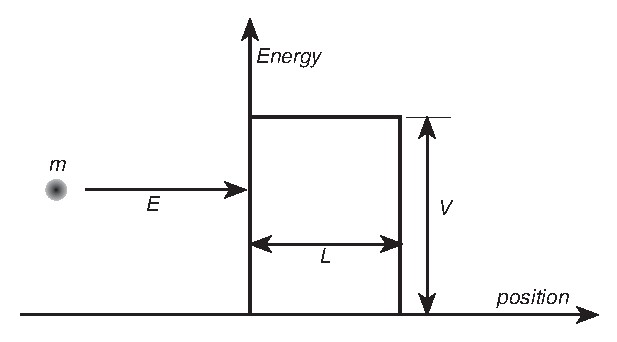
\includegraphics[]{QMBarrier}
% \epsfbox{Pix/QMBarrier.eps}
\end{center}
\caption{One Dimensional Barrier\label{QMBarrier:Fig}}
\end{figure}

This section demonstrates how an algebraic manipulation system might
be used to solve a problem in quantum mechanics that might arise in
practice, or at least in homework.  We wish to determine the
probability that a particle with mass $m$ and energy $E$ will pass
through the one dimension potential barrier given in
\figref{QMBarrier:Fig}.  This probability is called the {\em
transmission coefficient\/}.  We begin with the one dimensional, time
invariant Schr\"odinger equation:
\[
-{\hbar^2 \over 2 m} {d^2 \psi(x) \over dx^2} + V(x) \psi(x) = E
\psi(x).
\]
Here $\hbar = {h \over 2 \pi}$ where $h$ is Planck's constant.  The
mass of the particle is represented by $m$, and the energy by $E$.
The potential energy of the system is $V(x)$ and the wave function of
the particle is $\psi(x)$.

If the potential energy is constant we have
\[
{d^2 \psi(x) \over dx^2} + {2 m\,(E - V) \over \hbar^2} \psi(x) = 0.
\]
All solutions of this equation are linear combinations of two eigenfunctions
of the equations
\[
\psi(x) =  A e^{i \sqrt{2m\,(E - V)} x/ \hbar} + B e^{- i \sqrt{2m\,(E
- V)} x/ \hbar} 
\]
where $A$ and $B$ are arbitrary constants.  The first term in the sum gives
the probability amplitude of motion to the right (increasing $x$), while the
second term corresponds to motion to the left.  

We assume the height of the potential barrier is $V$ and that the
particle has energy $E$ with $E$ greater than $V$.
The barrier has has width $L$ and begins at $x=0$ and goes to
$x=L$.  We need to construct the wave function of a particle moving from
left to right and impinging on the barrier.  In each of the three regimes
$x<0$, $0<x<L$ and $L<x$, the potential is constant and thus the wave
function has the form given above.  We will use continuity conditions to
match the three wave functions at their boundaries.  This allows us to
determine the amplitudes of the wave functions.  We then compute the ratio
of the incoming amplitude and the outgoing amplitude.

We begin by setting two variables {\tt ALPHA} and {\tt BETA} to the wave
numbers of the particle outside the barrier and inside the barrier respectively
\begin{verbatim}
(C1) RADPRODEXPAND:FALSE$
\end{verbatim}
When {\tt RADPRODEXPAND} is set to true, expressions like $\sqrt{a b} /
\sqrt{a}$ will naturally simplify to $\sqrt{b}$ since the numerator will be
represented as $\sqrt{a} \sqrt{b}$.  We have set {\tt RADPRODEXPAND} to
false so that expressions like $\sqrt{2Em}$ will remain a single square
root as is conventional.
\begin{verbatim}
(C2) ALPHA:SQRT(2*M*E)/HBAR;
\end{verbatim}
\mdline{\sqrt{2Em} \over \hbar}{D2}
\begin{verbatim}
(C3) BETA:SQRT(2*M*(E-V))/HBAR;
\end{verbatim}
\mdline{\sqrt{2 m \,(E-V)} \over \hbar}{d3}
{\tt ALPHA} and {\tt BETA} are the two quantization constants that are
involved in the computation.  We use {\tt HBAR} to represent Planck's
constant.

\begin{verbatim}
(C4) A:1$

(C5) UL:A*%E^(%I*ALPHA*X)+B*%E^(-%I*ALPHA*X);
\end{verbatim}
\mdline{e^{i \sqrt{2Em} x / \hbar} + 
B e^{-{i \sqrt{2Em} x / \hbar}}}{D5}
This is the wave function to the left of the barrier.  Since the 
transmission coefficient is to be the ratio of $|A|^2$ and $|F|^2$, we
set {\tt A} to one here.  By eliminating this variable we reduce the number of
unknown variables to precisely the number of equations obtained by
fitting the pieces of the wave function together.
\begin{verbatim}
(C6) UC:C*%E^(%I*BETA*X)+D*%E^(-%I*BETA*X);
\end{verbatim}
\mdline{C e^{i \sqrt{2m\,(E-V)} x / \hbar}
+ D e^{-i \sqrt{2m\,(E-V)} x / \hbar}}{D6}
The wave function for the regime inside the potential barrier is similar,
but the wave number is different.
\begin{verbatim}
(C7) UR:F*%E^(%I*ALPHA*X);
\end{verbatim}
\mdline{F e^{i \sqrt{2Em} x / \hbar}}{D7}
Beyond the barrier we can assume that there is no reflection of the wave
at infinity.  Thus only one term is needed for the wave function.
\begin{verbatim}
(C8) UL-UC,X=0;
\end{verbatim}
\mdline{-D -C + B +1}{D8}
\begin{verbatim}
(C9) EQ1:%$

(C10) UC-UR,X=L$

(C11) EQ2:%$
\end{verbatim}
Since the wave function is continuous, the various pieces and their
derivatives must match up at the edges of the barrier.
\begin{verbatim}
(C12) EQ3:SUBSTITUTE(0,X,DIFF(UL-UC,X));
\end{verbatim}
\mdline{{i D \sqrt{2 m \, (E-V)} \over \hbar} -
{i C \sqrt{2 m \,(E-V)} \over \hbar} -
{i B \sqrt{2Em} \over \hbar}
+ {i \sqrt{2Em} \over \hbar}}{D12}
\begin{verbatim}
(C13) EQ4:SUBSTITUTE(L,X,DIFF(UC-UR,X))$
\end{verbatim}
These four expressions must be zero for the wave functions to be continuous
and have continuous derivatives.  The expressions are linear in the four
amplitudes, {\tt B}, {\tt C}, {\tt D} and {\tt F}.  Solving this system of
linear equations gives the value of {\tt F}.  We actually want 
the value of {\tt 1/F} since the transmission coefficient is the ratio of
those particles reflected by those which pass through the barrier.
\begin{verbatim}
(C14) SOLVE([EQ1,EQ2,EQ3,EQ4],[B,C,D,F])$

(C18) 1/F,%$
\end{verbatim}
This last quantity is too large to bother printing.  The probability
that particle will pass through the barrier is the magnitude of $F$
which can be determined by $F \overline{F}$, where $\overline{F}$ is the
complex conjugate of $F$.  {\Macsyma} does not have a  function that
computes the complex conjugate of an expression since the conjugate can
be determined by replacing all instances of $i$ in the expression by 
$-i$.  
\begin{verbatim}
(C19) SUBSTITUTE(-%I,%I,%)*%,RATSIMP;
\end{verbatim}
\mdline{e^{-{2 i L \sqrt{2Em-2mV} \over \hbar}}
\left( 
\begin{aligned}
    \displaystyle
    V^2 e^{4 i L \sqrt{2Em-2mV} / \hbar}\hfill\hfill\hfill\\
    \quad + \left( -2 V^2 + 16EV - 16E^2\right)e^{2 i L \sqrt{2Em-2mV} / \hbar}\\
    \quad +V^2
\end{aligned} \right)
\over 16EV - 16E^2}{D19}

The expression given in {\tt D19} is the transmission coefficient desired,
but is certainly not the expression normally given textbooks.  The next few
commands are devoted to simplifying {\tt D19}.  
\begin{verbatim}
(C20) (DEN:PART(%,2),NUM:PART(%,1))$

(C21) RATEXPAND(NUM);
\end{verbatim}
\mdline{
  \begin{aligned}
    V^2 e^{2 i L \sqrt{2Em -2mV} / \hbar}
      &+ V^2 e^{-{2 i L \sqrt{2Em -2mV} / \hbar}}\\
      &-2V^2 +16EV -16E^2
  \end{aligned}}{D21}
We would like to eliminate the complex exponentials.  We could apply
deMoivre's identity to {\tt D19} but a horrible mess of trigonometric
functions would result.  It would be quite difficult to cause {\Macsyma} to
produce the correct answer using that technique.  

The denominator already in roughly the form we would like.  To simplify some
of the steps that follow, we will deal with the numerator and denominators
separately. 
\begin{verbatim}
(C22) D21,DEMOIVRE,RATSIMP;
\end{verbatim}
\mdline{V^2 \left( 2 \cos {2 L \sqrt{2Em -2mV} \over \hbar} -2 \right)
+ 16 EV -16E^2}{D22}

The {\tt DEMOIVRE} command applies deMoivre's identity to {\tt D21}.  By
using {\tt RATSIMP} to simplify the expression the sine terms are caused to
cancel.  The coefficient of $V^2$ has the form $2 \cos 2 \theta - 2$.  We
next use the double angle formula to express {\tt D22} in terms of $\cos
\theta$.

\begin{verbatim}
(C23) ANS:EV(%/DEN,TRIGEXPAND);
\end{verbatim}
\mdline{
  \frac{
    \begin{aligned}
       V^2 \left( 2 \left( \cos^2 {L \sqrt{2Em -2mV} \over \hbar}
         - \sin^2 {L \sqrt{2Em -2mV} \over \hbar}\right) -2 \right)\qquad
         \hfill\\
       \hfill+ 16 EV -16E^2
    \end{aligned}}
    {16EV -16E^2}}{D23}
Unfortunately, {\Macsyma} uses the following double angle identity
\[
\cos 2\theta = \cos^2 \theta - \sin^2 \theta.
\]
By replacing $\cos^2 \theta$ by $1 - \sin^2 \theta$ the expression will be
reduced to a single trigonometric term.  The only problem is picking out
$\theta$.  

The {\tt PART} command in {\Macsyma} is used to out sub-expressions from
a larger expression.  Its first argument is the ``larger expression.''
The second argument says which part to return.  Thus given an
expression like
\[
w = x^2 + (2y - 1) x + 3
\]
{\tt PART($w$, 2)} is second argument to the top level sum, viz.,
$(2y-1) x$.  Successive {\tt PART} commands can be strung together by
additional selectors.  Thus {\tt PART($w$, 2, 1)} is $2y-1$ and so on.

For our problem, the following command will pick out the argument to the
cosine in $D23$.

\begin{verbatim}
(C24) PART(D23,1,1,2,1,2,1,1,1);
\end{verbatim} \mdline{{L \sqrt{2Em - 2mV} \over \hbar}}{D24}
\begin{verbatim}
(C25) SUBSTITUTE(1-SIN(D24)^2,COS(D24)^2,ANS);
\end{verbatim}
\mdline{{V^2\left(
2 \left(1 - 2\sin^2 {2L \sqrt{2Em-2mV} \over \hbar} \right)
 - 2\right)
+ 16EV - 16E^2 \over 16EV - 16E^2}}{D25}
{\Macsyma} likes to keep expressions as quotients of polynomials.  In this case
we would prefer to see the answer as $1 + <\hbox{quotient of polynomials}>$.
The following command does that. 
\begin{verbatim}
(C26) 1+FACTOR(RATSIMP(D25-1));
\end{verbatim}
\mdline{{\sin^2 \left({L \sqrt{2M (E - V)} \over \hbar}\right) V^2 \over 4E(E-V)} +1}{D26}
Thus the transmission coefficient for a particle impinging on a potential
barrier of height $V$ is
\[
1 + {\sin^2 {L \sqrt{2 m\,(E - V)} \over \hbar} V^2 \over 4 E \, (E - V)}.
\]
which is what we normally find in textbooks.

\section{Overview of the Algorithms and Capabilities}

As can be seen from these examples, algebraic manipulation systems can deal
directly with many of the quantities that arise in mathematics:
polynomials, rational functions, matrices and power series, for example.
Basic arithmetic operations with these types of objects can be implemented
relatively straightforwardly, however numerous performance complications
arise because of {\em intermediate expression swell\/}.  Arithmetic
operations with symbolic quantities tend to produce larger expressions from
smaller ones.  This distinguishes symbolic calculations from numeric ones
where numeric expressions tend not to grow in size.  Intermediate
expression swell occurs in a problem when the intermediate computations
swell to be much larger than the final answer.  A prime example of this
problem occurs when calculating polynomial GCD's.  These issues are
discussed in some detail in \chapref{Poly:Arith:Chap} and some approaches
to their solution are given in Chapters \ref{Interpolation:Chap} and
\ref{Hensel:Chap}. 

Symbolic systems are more likely to deal with infinite structures such as
ideals, lattices or power series, than numerical systems.  We want to perform
the same types of operations on these structures as on simpler structures.
In \chapref{Ideal:Arithmetic:Sec}.

There are certain additional operations that are possible with symbolic
quantities.  \Marginpar{orthogonal functions expansions, analysis of
singularities} 
Some operations that are impractical for numerical quantities
turn out to be quite cheap for symbolic expressions.  For instance,
there is no known polynomial time algorithm for factoring integers, and
more to the point it is quite hard in practice to factor integers.
However, there do exist polynomial time algorithms for factoring
polynomials, and in practice polynomials are relatively easy to
factor.\footnote{The distinction between practice and theory is made here
because the polynomial time algorithm is an $O(n^{12})$ algorithm, while
the exponential algorithms which are used in practice  usually only 
require $O(n^{3})$ operations.}

Another	aspect of symbolic computation is exact versus inexact computation.

Where there are similarities between numerical and symbolic calculations,
the introduction of symbolic parameters often allows one to examine a wide
variety of possibilities with a single computation.

Groups, Fields, Riemann surfaces, topological structures, etc as first
class objects.

Computations: arithmetic, solving systems of equations, approximation
techniques, etc.


Problems: simplification: definite canonical and normal simplifiers.




\section{Where Current Research is Heading}

With some exceptions the contents of this book are largely classical.
The algorithms discussed are solutions to the problems set out by
parents of the Computer Algebra field at the end of the 1960's.  Since
then, much has changed.  The massive increase in performance of computer
systems and their precipitative drop in price has changed many of the
premises upon which computer algebra research is based.



\part{Number Theory}
    %$Id: euclids-alg.tex,v 1.1 1992/07/12 19:39:34 rz Exp rz $
\chapter{Euclid's Algorithm}
\label{Integer:GCD:Chap}

Among the mathematical problems we will investigate is the computation
of greatest common divisors, factoring into prime factors and finding
rational approximations.  These computations may be performed on a
variety of different mathematical quantities: polynomials, rational
integers, power series, differential operators, etc.  The most
familiar of these algebraic structures are the \keyi{natural numbers}:
$\mathbb{N} = \{1, 2, 3, \ldots\}$.  If we include zero and 
the negative integers we have $\Z$, the ring of \keyi{rational
integers}. The elements of $\Z$ are commonly called the  
\keyi{integers}, but we will use the term integer for more complex
algebraic structures. 
\addsymbol{$\mathbb N$}{The natural, or counting numbers, $1, 2, 3, \ldots$}
\addsymbol{$\Z$}{The ring of rational integers}
\addsymbol{$\Q$}{The field of rational numbers}

This chapter begins our study of mathematical algorithms with an
investigation of a variety of computations involving the rational
integers.  Later chapters discuss more elaborate algorithms that deal
with polynomials and other algebraic structures.  Interestingly, the
resolution of some of these problems for the rational integers can
lead to algorithms that make use of polynomials, thus making the whole
process somewhat circular.

\medskip
An integral part of our elementary education is learning to add and
multiply integers.  The hardware used in computers usually only
implements arithmetic operations for numbers of a specified length,
\ie, $32$-bit or $64$-bit integers.  In algebraic computation we often
use much larger integers; however, this is not because the answers are
so large.  Instead these large numbers arise in the middle of some
computation and then shrink towards the end.  This phenomenon is
called \keyi{intermediate expression swell}.

Detailed algorithms for integer arithmetic may be found in many texts,
\eg, {\Knuth} \cite{Knuth1997-tf} and {\Aho}, {\Hopcroft} and {\Ullman}
\cite{Aho1974-yy}. But implementing efficient variable
precision arithmetic algorithms is a very delicate process that raises
many issues not touched upon in these texts, such as register usage,
cache turbulence and pipeline stalls.  For instance, properly
implemented classical algorithms work very well for larger integers
than one might expect.  Because of all of these reasons, because
numerous variable precision integer packages are available and because
an increasing number of programming languages now provide variable
precision integers as one of their basic types, we do not discuss
these arithmetic algorithms.

\medskip
We begin with some basic definitions.  When a rational integer $m$ can
be written as a product of two other integers $p$ and $q$, $m = pq$,
then $p$ and $q$ are called {\em divisors}\index{divisor} of $m$ and
$m$ is said to be {\em divisible} by $p$ and
$q$.\index{divisibility!integer} We write $p \mid m$ to indicate that
$p$ divides $m$.  We indicate that $p$ does not divide $m$ by $p \nmid
m$.  The only rational integers that have multiplicative inverses are
$1$ and $-1$.  Because they have multiplicative inverses they are
called {\em units}.\index{unit, of a ring} Two integers whose ratio is
a unit are said to be \keyi{associates}.  For simplicity we will
ignore associates when enumerating the divisors of an integer.  Thus
every non-unit has at least two divisors, $1$ and itself (up to
associates).  An integer that has only these two ``trivial''
divisors\index{trial division} is called a \keyi{prime}.  All other
non-units are called \keyi{composite}.
\addsymbol{$p \mid m$}{$p$ divides $m$}
\addsymbol{$p \nmid m$}{$p$ does not divide $m$}

A presentation of a positive integer $N$ as a product of positive
integers, $N = m_1 \cdots m_k$, is called a \keyi{factorization} of
$N$.  A factorization of an integer is said to be {\em
complete}\index{factorization!complete} if each of the $m_i$ is a
prime or a power of a prime.  Unless otherwise noted, all
factorizations are complete.  We usually write such factorizations as
$N= p_1^{e_1} \cdots p_k^{e_k}$.  According to the
\key{fundamental theorem of arithmetic} the factorization of a
rational integer is unique.

The factoring problem for an integer $N$ is, at the moment, very
difficult.  Trying all possible divisors takes time $O(\sqrt{N})$.
Very roughly, the best known algorithms take time $O(\exp(\sqrt{\log
N}))$, which, though much better, is not near what would be expected
of a polynomial time algorithm: $O(\log^k N)$.  Interestingly, the
time required to factor a polynomial of degree $n$ is only about $O(n^5)$.

An integer $d$ that divides both $m$ and $n$ is called a \keyi{common
divisor} of $m$ and $n$.  The number $m/d$ is called the
\keyi{cofactor} of $m$ with respect to $d$.  The largest common
divisor of two integers is called a \keyi{greatest common divisor}
({\sc gcd}).  If the greatest common divisor of two integers is $1$,
then we say they are {\em relatively prime\/}.\index{relatively prime}
When dealing with rational numbers, more time is probably spent
computing the {\sc gcd} of integers than any operation other than
addition and multiplication.  When using rational functions, it is not
unusual for the time spent computing polynomial {\sc gcd}s to dominate
all other arithmetic operations.  \sectref{Integer:Euclidean:Sec}
discusses Euclid's algorithm for computing the {\sc gcd} of two
integers.  Euclid's algorithm provides an entr\'e to many facets of
elementary number theory.  The other sections of this chapter
illustrate several of these ideas.  Later chapters delve into each of
the issues raised in more detail.

\section{Euclidean Algorithm}
\label{Integer:Euclidean:Sec}

\index{Euclidean algorithm|(}
The {\em Euclidean algorithm} for computing the {\sc gcd} of two
integers has been known at least from the time of \key{Euclid}
\cite{Fritz1945-sw}, who called it ``\key{anthyparesis}.''  Most
likely, it is the oldest mathematical algorithm in existence.  The
principles underlying the Euclidean algorithm are fundamental to the
solution of many problems in mathematics ranging from diophantine
approximation to elimination.  Because of its importance, and because
it is the first algorithm we consider, we derive Euclid's algorithm in
some detail.

Let $m > n$ be two positive rational integers.  Denote by $d$ some
common divisor of $m$ and $n$.  $d$ also divides, $m+n$ and $m-n$.  In
fact, $d$ divides every number of the form $am - bn$, where $a$ and
$b$ are rational integers.  Denote by $M$ the set of all such numbers
\[
M = \{ am - bn \mid a,b \in \Z\}.
\]
Since every common divisor of $m$ and $n$ divides every element of
$M$, each is also a multiple of the greatest common divisor of $m$ and
$n$.  Thus the smallest positive element of $M$ is the {\sc gcd} of $m$ and
$n$.

To make this an algorithm, we use a simple recursive technique that
converts a pair of elements in $M$ into a pair of smaller elements.
This process terminates with the pair $0$ and the {\sc gcd} of $m$ and
$n$.  The simplest approach is to replace the pair $(m,n)$ by
$(m-n,n)$, and then $(m-2n, n)$, and so on until $m-kn < n$.  At this
point the two values are interchanged and the new pair is $(n, m-kn)$.

\index{remainder}
All of the subtraction operations prior to an interchange of $m-n$ and
$n$ can be collapsed into a single division:
\begin{equation}
m = q n + r.\qquad\qquad 0 \le r < n 
\label{Remainder:Eq}
\end{equation}
In this case, $r$ is called the {\it remainder} of $m$ divided by $n$.
(This definition works both for positive and negative values of $m$
and $n$.)  Now let $n_1 = m$ and $n_2 = n$.  The sequence of
divisions and remainders used in the {\sc gcd} algorithm would look like:
\begin{equation} \label{Int:RemainderSeq:Eq}
  \begin{aligned}
   n_1 &= q_1 n_2 + n_3\\
   n_2&=q_2 n_3 + n_4\\
     &\vdots\\
   n_k& = q_k n_{k+1} + 0
  \end{aligned}
\end{equation}
This sequence of operations is called a \keyi{remainder sequence}, and
its use to compute the {\sc gcd} of two numbers is called Euclid's
algorithm.  \figref{Int:Euclid:Alg:Fig} illustrates the computation of
the {\sc gcd} of $15027133$ and $8562227$.  In this case the {\sc
gcd} is $163$ which we write as 
\[
(10527133, 8562227) = 163.
\]

\begin{figure}
\[
\begin{aligned}
  15027133 &= 1 \cdot 8562227 + 6464906\\
  8562227  &= 1 \cdot 6464906 + 2097321\\
  6464906  &= 3 \cdot 2097321 + 172943\\
  2097321  &= 12 \cdot 172943  + 22005\\
  172943   &= 7 \cdot 22005   + 18908\\
  22005    &= 1 \cdot 18908   + 3097\\
  18908    &= 6 \cdot 3097    + 326\\
  3097     &= 9 \cdot 326     + 163\\
  326      &= 2 \cdot 163     + 0
\end{aligned}
\]
\caption{Euclidean algorithm for two integers\label{Int:Euclid:Alg:Fig}}
\end{figure}


The following recursive function gives a direct implementation of the
Euclidean algorithm for two positive integers, based on the discussion
of the previous few paragraphs.

\begin{lstlisting}[language=Python]
def IntGcd(m, n) -> int:
  if m < n:
    return IntGcd(n, m)
  elif n == 0:
    return m
  else:
    return IntGcd(n, m % n)
\end{lstlisting}

The bulk of the work is performed in the remainder calculation.  For
some machines, it may be substantially cheaper to compute something
slightly larger than the remainder.  For instance, the first several
bits of $m$ and $n$ allow us to estimate the size and first few bits
of the quotient of $m$ and $n$ quickly.  Using this value, something
close to the remainder can be computed quite quickly.  Other
algorithms are described in Section 4.5.2 of {\Knuth} \cite{Knuth1997-tf}.

The second question we have about every algorithm is: How fast is it?
(The first question is whether or not the algorithm gives the correct
answer!)  To answer this question we bound the number of remainder
steps required 
to compute the {\sc gcd} of two integers.  Denote by $F(N)$ the
maximum number of 
remainder steps required to compute the {\sc gcd} of two positive
numbers less than $N$.

Assume $u > v$ are two positive integers without a common factor, each
larger than $N$ and chosen such that the quotients in their remainder
sequence are all $1$.  Thus, the {\sc gcd} of two integers smaller
than $N$ cannot take any more steps than the number required by $u$
and $v$.  The pair of integers $u+v$ and $u$ also has a remainder
sequence where each $q_i$ is $1$, and the remainder sequence for
$(u+v, u)$ is one step longer than that for $(u, v)$.  The sequence
$v, u, u+v, 2u+v,
\ldots$, can be continued as far as one would like.

To obtain a bound on the number of steps in a {\sc gcd} algorithm, we need
to be able to compute the growth rate of the terms of this sequence.
A crude bound can be determined by the following simple reasoning.

Assume that when the Euclidean algorithm is applied to two integers
$F$ and $G$, $F > G$, the remainder sequence is as long as possible.
For this to be the case, the quotient of $F$ divided by $G$ should be
$1$.  Denote the remainder by $H$.  For $F$ and $G$ to have a long
remainder sequence $G$ and $H$ must also.  Thus the quotient of $G$
divided by $H$ should also be one.  This suggests that we should
consider the sequence of numbers $f_i$ satisfying the 
recurrence
\begin{equation}
\label{Fibonacci:Eq}
f_{i+1} = f_i + f_{i-1},
\end{equation}
where we can take the basis of the \keyi{difference equation} to be $f_{1} =
f_{2} = 1$.  $f_i$ has a remainder sequence of length $i-1$ when
divided by $f_{i-1}$ and no smaller number can have a remainder
sequence so long.\label{Fibonacci:Remainder:Sequence}

Since the integer quotient of $f_{i}$ divided by $f_{i-1}$ is $1$,
$f_{i} < 2 f_{i-1}$.  This allows us to bound $f_{i+1}$ above and
below as follows:
\[
3 f_{i-1} > f_{i+1} > \frac{3}{2} f_{i},
\quad\mbox{or}\quad
c_1\left(\sqrt{3}\right)^i > f_{i+1} > c_2 (\frac{3}{2})^{i}.
\]
Consequently,
\[
F(N) = O(\log N).
\]

We can improve the constants in the estimates for $f_{i+1}$ above with
only a bit more work.  Assume that for large $i$ the ratio between
$f_{i+1}$ and $f_i$ tends to a constant, $\phi$.  Then for sufficiently
large $n$ we have 
\[
\phi = \frac{f_{n+1}}{f_n} = \frac{f_n + f_{n-1}}{f_n} = 1 + \frac{1}{\phi}.
\]
This gives a quadratic equation for $\phi$, $x^2 - x - 1=0$, whose
only positive solution is
\[
\phi = \frac{1 + \sqrt{5}}{2} \approx 1.618033988749894.
\]
So we expect $f_i = c_1 \phi^i$.  
Notice that this lies between the bounds given above of $\sqrt{3} =
1.732$ and $3/2 = 1.5$.  

We can go further and determine an exact formula for $f_i$.  Notice that if
$\alpha$ is a zero of $x^{2} -x -1$ then $\alpha^{i}$ will satisfy
\eqnref{Fibonacci:Eq}: 
\[
f_{i+1} - f_{i} - f_{i-1} = \alpha^{i+1} - \alpha^{i} - \alpha^{i-1}
 = \alpha^{i-1} ( \alpha^{2} - \alpha -1) = 0.
\]
Since \eqnref{Fibonacci:Eq} is a linear \key{difference equation},
linear combinations of the solutions of \eqnref{Fibonacci:Eq} are also
solutions.  The negative solution of the quadratic equation is $1-\phi
= -1/\phi$. Consequently,
\[
f_i = c_1 \phi^i + c_2 (-\phi)^{-i},
\]
where, as with ordinary differential equations, $c_1$ and $c_2$ are
determined by the ``initial conditions.''  Using $i = 1$ and $i=2$ we
have
\[
\begin{aligned}
  c_1 \phi - c_2 \phi^{-1} &= f_{1} = 1,\\
  c_1 \phi^2 + c_2 \phi^{-2}&= f_{2} = 1,
\end{aligned}
\]
whose solution is
\[
\begin{aligned}
  c_1 &= \frac{\phi +1}{\phi^3 +\phi} = \frac{1}{\sqrt{5}},\\
  c_2&=\frac{\phi^2 - \phi^3}{\phi^2 + 1} = - \frac{1}{\sqrt{5}}
\end{aligned}
\]
Thus,
\[
f_i = 
\frac{1}{\sqrt{5}} \left[
\left(\frac{1 + \sqrt{5}}{2}\right)^i -
        \left(\frac{1 - \sqrt{5}}{2}\right)^i \right]
\]

This sequence of numbers is called the \keyi{Fibonacci numbers}.  They
were first mentioned by {\Fibonacci} \cite[pages 283--285]{Pisano1857-nc}
and have important applications in number theory, complexity theory
and other fields.

Since the negative solution of the quadratic equation has absolute
value less than $1$, for large $i$, the Fibonacci numbers can be
approximated by
\[
f_i = \frac{\phi^i}{\sqrt{5}}
\]
for large $i$. Consequently,
\[
F(N) \approx \frac{\log \sqrt{5} N}{\log \phi} = \log_{\phi} \sqrt{5} N.
\]
These results were first demonstrated  by {\Lame} in 1844 \cite{Lame1844-wm}.

The techniques used to solve this simple \key{difference equation} are
similar to those used to solve constant coefficient linear
differential equations.  More complicated difference equations often
occur when analyzing algorithms and in other problems.  Obtaining
closed form and asymptotic solutions of difference equations is
somewhat similar to the corresponding problems for differential
equations where symbolic techniques have had dramatic success in
recent years.  The field of difference equation problems has not been
as closely examined and remains a fertile area for future research.

\index{Euclidean algorithm|)}

\section{Diophantine Approximations}
\label{Euclid:DA:Sec}

Returning to the original problem, assume we are interested in
computing the {\sc gcd} of $n_1$ and $n_2$.  For simplicity we assume
the {\sc gcd} is $1$.  Define $M$ to be the set
\[
M = \{ n_1 X - n_2 Y \mid X, Y \in \Z \}.
\]
The {\sc gcd} of $n_1$ and $n_2$ is the smallest positive element of $M$.
In other words, we want to find the smallest non-trivial value of the
binary form $|n_1 X - n_2 Y|$.  Another way to say this, is that we want
to find the best possible rational number approximation to $n_1/n_2$:
\[
\left|\frac{n_1}{n_2} - \frac{Y}{X}\right| \le \frac{1}{n_2 X} < \frac{1}{X^2}.
\]

Looking closely at the remainder sequence\index{remainder
sequence!integer} \eqnref{Int:RemainderSeq:Eq}, we can see how to find
the candidate solutions $X$ and $Y$.  By isolating the remainder terms
on one side of the equation we have
\[
  \begin{aligned}
    n_1 - q_1 n_2 &= n_3,\\
    n_2 - q_2 n_3 &= n_4,\\
     &\vdots\\
    n_{k-1} - q_{k-1} n_{k} &= 1.
  \end{aligned}
\]
We can substitute the value of $n_3$ given in the first equation into
the second equation, to get a relationship between $n_1$, $n_2$ and
$n_4$:
\begin{equation}\label{Euclid:Int:D:Eq}
-q_2 n_1 + (q_1 q_2 + 1) n_2 = n_4.
\end{equation}
Writing this relation in the form of an approximation to $n_1/n_2$  gives
\[
\left|\frac{n_1}{n_2} - \frac{q_1 q_2 + 1}{q_2}\right| 
= \frac{n_4}{n_2 q_2}.
\]

Using \eqnref{Euclid:Int:D:Eq}, and $n_3 = n_1 - q_1 n_2$, we can
obtain a relationship between $n_1$, $n_2$ and $n_5$:
\[
\left|\frac{n_1}{n_2} - \frac{q_1 q_2 q_3 + q_1 + q_3}{q_2 q_3 +1 }\right| 
= \frac{n_5}{n_2 (q_2 q_3 +1)}.
\]
Notice that 
\[
\frac{n_4}{n_2 q_2} > \frac{n_5}{n_2 (q_2 q_3 +1)},
\]
so the Euclidean algorithm is actually producing increasingly accurate
approximations to $n_1/n_2$.

When this process is taken to its logical conclusion, one obtains two
polynomials $X$ and $Y$ in the quotients $q_1, \ldots, q_{k-1}$ such
that
\[
 n_1 X - n_2 Y = 1,
\]
since $n_1$ and $n_2$ are relatively prime.  $Y/X$ is a quite
good approximation to $n_1/n_2$:
\[
\left|\frac{n_1}{n_2} - \frac{Y}{X}\right| = \frac{1}{n_2 X} 
   <  \frac{1}{X^2}.
\]
Observe that fractions with a denominator of $X$ can only approximate
real numbers to an accuracy of $1/2X$.  

The problem just studied can be phrased as trying to minimize the
value of the form $X r - Y$, where $r$ is a rational number.  There are
many interesting generalizations.  If $r$ is replaced by an algebraic
number, then it turns out that there are an infinite number of
``exceptionally'' good approximations to $r$ if $r$ is the solution of
a quadratic equation with integer coefficients, but only a finite
number of such solutions when $r$ is of higher degree.

It is also interesting to consider multiple approximations.  Given
real numbers $\alpha_1, \alpha_2, \ldots, \alpha_k$, we would like to
find integers that minimize the linear form:
\[
\left|X_0 + X_1 \alpha_1 + X_2 \alpha_2 + \cdots + X_k \alpha_k \right|.
\]
This type of problem is discussed in \chapref{Lattice:Chap} and can be
used to develop theoretically efficient algorithms for factoring
polynomials.

\section{Continued Fractions}
\label{Euclid:CF:Sec}

The approximation ideas of the previous section can be further developed
by rewriting the remainder sequence \eqnref{Int:RemainderSeq:Eq} in terms
of fractions.  This gives:
\begin{equation}\label{Euclid:CF:Eq}
  \begin{aligned}
    \frac{n_1}{n_2} &= q_1 + \frac{n_3}{n_2},\\
    \frac{n_2}{n_3} &= q_2 + \frac{n_4}{n_3},\\
     &\vdots\\
    \frac{n_{k-1}}{n_k} &=  q_{k-1} + \frac{1}{n_k}.
  \end{aligned}
\end{equation}
Replacing $n_3/n_2$ by the value in the second of these equations,
and continuing we have:
\[
\begin{aligned}
\frac{n_1}{n_2} &= q_1 + \frac{n_3}{n_2} = 
 q_1 + \frac{1}{\displaystyle q_2 + \frac{n_4}{n_3}}, \\
& = \frac{n_1}{n_2} = q_1 + \frac{1}{\displaystyle q_2 + 
    \frac{1}{\displaystyle q_3 + 1 \frac{1}{\displaystyle q_4 +
\ddots}}}.
\end{aligned}
\]
This strange way of writing the fraction $n_1/n_2$ is called a
\keyi{continued fraction}.   The $q_i$ that appear in the continued
fraction are called the {\em partial quotients}.\index{partial
quotient} From
\eqnref{Euclid:CF:Eq} and using the fact that $n_1 > n_2 > n_3 >
\cdots$ we see that  $q_i$ is the integer part of $n_i/n_{i+1}$.

Truncating the continued fraction and clearing the denominators:
\[
\begin{aligned}
q_1 + \frac{1}{q_2} & = \frac{q_1 q_2 + 1}{q_2}, \\
q_1 + \frac{1}{\displaystyle q_2 + 
    \frac{1}{\displaystyle q_3}} & = 
  \frac{q_1 q_2 q_3 + q_1 + q_3}{q_2 q_3 + 1}.
\end{aligned}
\]
Notice that these are the ``exceptionally'' good approximations to
$n_1/n_2$ discovered earlier.  This property is one of the reasons for
the interest in continued fractions.  \chapref{CF:Chap} discusses some
of the properties of continued fractions in more detail and how to
perform calculations with them.

\section{Diophantine Equations}
\label{Euclid:DE:Sec}

If we are only interested in the integral (or perhaps rational)
solutions of a polynomial equation (or system of equations), then we
call the problem a {\em diophantine} problem.\index{diophantine
equation} The simplest diophantine equation has already appeared.  To
compute the best rational approximation of $n_1/n_2$ we were looking
for integers $X$ and $Y$ such that
\begin{equation}\label{Euclid:Approx:Eq}
n_1 X - n_2 Y = 1.
\end{equation}
This is a  diophantine equation in $X$ and $Y$ since only elements of
$\Z$ are of interest in its solution.

This equation does have an infinite number of solutions, however.  Let
$x$ and $y$ be a solution of \eqnref{Euclid:Approx:Eq}.  Then $x+n_2
t$ and $y+ n_1 t$ is also a solution for integral values of $t$.  Thus
there are a countable number of solutions to \eqnref{Euclid:Approx:Eq}
as a diophantine problem.

Diophantine equations arise in a number of problems.  We give two more
examples here.  An integral \keyi{Pythagorean triangle} is a right
triangle (in Euclidean space) whose sides are each rational integers.
By the Pythagorean theorem their sides are zeroes of
\[
x^2 + y^2 = z^2,
\]
where $z$ is the length of the hypotenuse.  This equation involves three
unknown variables and is quadratic, not linear.  As an equation over
the reals, it has a continuously infinite number of solutions.  As a
diophantine equation, it has only a countably infinite number of
solutions, which can be parameterized as 
\begin{equation}\label{PythagEq:Soln:Eq}
x = r^2 - s^2, \quad y = 2rs, \quad z = r^2 + s^2.
\end{equation}
We leave the proof of this to the reader.  

What integers can arise as the sides of a Pythagorean triangle?  Any
even integer, \eg, $2k$ can be a side:
\[
(k^2 - 1 , 2k, k^2+1).
\]
Odd integers can also be sides, since every odd number is the difference
of two squares, $2k+1 = (k+1)^2 - k^2$.  Thus,
\[
(2k+1, k(k+1), 2k^2+2k +1)
\]
is a Pythagorean triple.

A more challenging question is: Which rational integers can be the
{\em area} of a Pythagorean triangle?  If the sides of the triangle
are restricted to be rational integers then the area must be of the
form $rs(r^2-s^2)$.  However, it is more interesting to consider
triangles whose sides are rational numbers and whose area is an
integer.\Marginpar{Need to give an example here and give a bit more detail.}

Pythagorian triangles with rational sides can be determined by
allowing $r$ and $s$ to be rational in \eqnref{PythagEq:Soln:Eq}.  (Do
all Pythagorean triangles with rational sides arise in this fashion?)

The integer $n$ is the area of a Pythagorean triangle if $xy = 2n$ and
$x^2 +y^2 = z^2$.  Eliminating $y$ we have
\[
x^2 + \left(\frac{2n}{x}\right)^2 = z^2 \Longrightarrow x^4 + 4n^2 =
(xz)^2.
\]
Rewriting this slightly, we want to know if there exist rational
numbers $u$ and $v$ such that
\begin{equation}\label{Euclid:Cong:Eq}
u^2 = v^4 + 4n^2.
\end{equation}
This is a far harder diophantine equation to solve.  In this case
there are only a finite number of solutions and proving this is quite
difficult.  To do so requires techniques of {\em elliptic
curves}.\index{elliptic curve} This problem is beyond the grasp of the
techniques discussed in this book.  A nice presentation of the
mathematics relevant to this problem and its solution is given in
{\Koblitz}'s book \cite{Koblitz2012-wq}.

\section*{Notes}

\small

If $F$ is a purely algebraic extension of the rational numbers, $\Q$,
then every element $\alpha \in F$ is the zero of a polynomial with
coefficients in $\Z$.  If $\alpha$ is the zero of a polynomial whose
\key{leading coefficient} is $1$ then $\alpha$ is said to be an
\keyi{integral element} of $F$.  The ring of integral elements of $F$
is called the \keyi{ring of integers} of $F$.  The ring of integers of
$\Q[\sqrt{-1}]$ is $\Z[\sqrt{-1}]$ and the elements of $\Z[\sqrt{-1}]$
are called \keyi{Gaussian integers}.  The ring of integers of
$\Q[\sqrt{5}]$ is $\Z[(1+\sqrt{5})/2]$.

The integral elements of $\Q$ are the elements of $\Z$.  Throughout
this book we use the term \keyi{rational integer} instead of just {\em
integer} to be more precise.

\normalsize

    %$Id: cont-frac.tex,v 1.2 1992/05/10 19:34:57 rz Exp rz $
\chapter{Continued Fractions} 
\label{CF:Chap}

\def\Ddots{\mbox{\raisebox{-2ex}{$\ddots$}}}
\index{continued fraction|(}


By a \keyi{continued fraction} we mean an expression of the form
\[
a_0 + \frac{b_1}{\displaystyle a_1 + \frac{b_2}{\displaystyle a_2 + \Ddots}}\ .
\]
When this expression is finite, it represents a rational number. The
infinite form of of the continued fraction is defined to be the 
limiting value of the sequence 
\[
a_0, \quad a_0 + \frac{b_1}{a_1}, \quad 
a_0 + \frac{b_1}{\displaystyle a_1 + \frac{b_2}{a_2}}, \quad \ldots,
\]
if the limit exists.  Assume the limit does exist, and denote it by
$\alpha$.  The elements of this sequence are called the  
{\em continued fraction convergents}\index{convergents!of a continued
fraction} of $\alpha$.  When the $b_i$ are equal to 1, the 
elements of the above sequence are quite good approximations to
$\alpha$ and, in a certain sense, all of the ``best'' approximations
to $\alpha$ are elements of the sequence.

The major goal of this chapter is to make these concepts precise and
to provide algorithms for determining these convergents efficiently.
These results will provide efficient algorithms for solving certain
diophantine problems.

\section{Basics}
\label{CF:Basics:Sec}

We consider only continued fractions where the numerators are $1$,
\ie, fractions of the form
\[
a_0 + \frac{1}{\displaystyle a_1 + \frac{1}{a_2 + \Ddots}},
\]
and where the $a_i$ are positive integers.  A continued fraction of
this form is called a {\em simple continued
fraction\/}\index{continued fraction!simple}.  To simplify the
notation, simple continued fractions are written as
\[
a_0 + \frac{1}{\displaystyle a_1 + \frac{1}{a_2 + \Ddots}}
    = [a_0,a_1, a_2, \ldots].
\]
The $a_i$ are called the {\em partial quotients}\index{partial
quotient} of the continued fraction.  The $n$-th {\em
convergent}\index{continued fraction!convergent} of a continued
fraction is defined as:
\[
\frac{P_n}{Q_n} = [a_0, a_1, \ldots, a_n].
\]
\addsymbol{$[a_0, a_1, \ldots]$}{Continued fractions with partial
quotients $a_i$}

Let $\alpha = [a_0, a_1, \ldots]$, where only the finite
series is well defined at this time.  Notice that the expression
\[
\frac{1}{\displaystyle a_1 + \frac{1}{a_2  + \Ddots}}
\]
is always positive and less than $1$.  Therefore, $a_0$ is the
\key{integer part} of $\alpha$, which we denote by 
$\lfloor \alpha \rfloor$.  (We use $\lceil \alpha \rceil$ to denote
the smallest integer greater than or equal to $\alpha$.)  The second
partial quotient is
\[
a_1 = \left\lfloor \frac{1}{\alpha - a_0} \right \rfloor = \lfloor
\alpha_1 \rfloor,
\]
and so on. 
\addsymbol{$\lfloor \alpha \rfloor$}{The greatest integer less than or
equal to $\alpha$}
\addsymbol{$\lceil \alpha \rceil$}{The smallest greatest integer
greater than or equal to $\alpha$}


If $\alpha$ is a rational number, this process will terminate with a
finite simple continued fraction of the form
\[
\alpha = [a_0, a_1, \ldots, a_n ] = [a_0, a_1, \ldots, a_n -1, 1],
\]
where the last step is a reflection of the identity
\[
k = (k-1) + \frac{1}{1}.
\]
Any finite continued fraction represents a rational number, so 
irrational numbers have infinite continued fractions expansions.
These expansions are unique, the proof of which we leave to the
reader.  We summarize these results in the following proposition.

\begin{proposition}
Let the simple continued fraction expansion of $\alpha$ be
\[
\alpha = [a_0, a_1, \ldots, a_k, \ldots ].
\]
If $\alpha$ is irrational this expansion will not terminate and it is
unique.  If $\alpha$ is rational, then it has precisely two simple
continued fraction expansions and they are related as follows
\[
\alpha = [a_0, a_1, \ldots, a_n] = [a_0, a_1, \ldots, a_n-1, 1].
\]
Thus a rational number has a unique continued fraction expansion with
an even number of partial quotients and a unique continued fraction
expansion with an odd number of partial quotients.

\end{proposition}

\bigskip
A good example of the types of approximations produced by continued
fractions  is given by $\pi$.  Apply the procedure given above
to $\pi$ (using a calculator, for instance) gives
\[
\begin{array}{rlc}
\alpha = \pi &= 3.141592653589793\ldots & a_0 = 3 \\
\alpha_1 = (\pi - 3)^{-1} &= 7.062513305931052\ldots 
   & a_1 = 7 \\
\alpha_2 = (\alpha_1 - 7)^{-1} &= 15.996594406684104\ldots 
   & a_2 = 15 \\
\alpha_3 = (\alpha_2 - 15)^{-1} &= 1.0034172310150003\ldots 
   & a_3 = 1 \\
\vdots  & \vdots 
\end{array}
\]
When computed with enough precision, we discover that
\[
\pi = [3,7,15,1,292,1,1,1,2,1,3,1,14,2,1,1,2,2,2,2,1,84, \ldots].
\]
The resulting convergents are 
\[
3,\quad \frac{22}{7},\quad \frac{333}{106},\quad \frac{355}{113},
  \quad \frac{103993}{33102}.
\]
The first convergent is the Biblical value for $\pi$, the second is
the value often used in hand calculations prior to the appearance of
the calculator, and the fourth is well known as being an exceptionally
accurate value for a fraction with such a small denominator---its
error is less that $10^{-6}$.  In general, the convergent before a
particularly large partial quotient will be especially
accurate.\index{$\pi$, biblical value}

The numerical values of the continued fraction convergents of $\pi$ given
above are
\[
3.0,\quad 3.142857, \quad 3.141509, \quad 3.141593, \quad 3.1415926.
\]
Notice that these approximations are alternately larger and then smaller
than $\pi$.  This is true of all simple continued fractions, as we
shall prove in \propref{CF:Convergence:Prop}.

\bigskip

To simplify some of the notation that follows it is convenient to add two
extra convergents to the set derivable from the continued fraction.  The value
of a simple continued fraction is always less than $\infty$ and greater than
0.  We can preserve the alternating behavior of the convergents by letting
the $-1${\st} convergent be $1/0$ and the $-2$-nd be $0/1$.

The first few convergents of a continued fraction
$[a_0, a_1, a_2, \ldots]$ are thus
\[
\begin{array}{c|ccccc}
    n & -2 & -1 & 0 & 1 & 2 \\ \hline\noalign{\vspace{2pt}}
    \displaystyle\frac{P_n}{Q_n} & \displaystyle\frac{0}{1}& \displaystyle\frac{1}{0}&
    \displaystyle\frac{a_0}{1}& \displaystyle\frac{a_0 a_1 + 1}{a_1} &
    \displaystyle\frac{a_0 a_1 a_2 + a_2 + a_0}{a_1 a_2 + 1}
\end{array}
\]
These examples suggest that the convergents of a continued fraction
satisfy the following simple pair of recurrence relations:
\begin{equation}
\label{CFRecurrence:Eq}
 \begin{aligned}
  P_{n+1} &= a_{n+1} P_n + P_{n-1},\\
  Q_{n+1} &= a_{n+1} Q_n + Q_{n-1}.
 \end{aligned}
\end{equation}
This is in fact the case and will be shown in
\propref{CF:Recurrence:Prop}. First, we show that sequences that
satisfy \eqnref{CFRecurrence:Eq} satisfy certain identities.

\begin{proposition}\label{CF:Identities:Prop}
If $P_k/Q_k$ satisfy the relations \eqnref{CFRecurrence:Eq} then 
\begin{align}
  P_n Q_{n-1} - P_{n-1} Q_n &= (-1)^{n-1}, \label{CFUnitIdentity:Eq} \\
  P_n Q_{n-2} - P_{n-2} Q_n &= a_n(-1)^{n}. \label{CF:2Dif:Identity:Eq} 
\end{align}
\end{proposition}

\begin{proof}
The first identity is easily shown using induction.  Equation
\eqnref{CFUnitIdentity:Eq} is true for $n= 0, 1$.  Assuming
\eqnref{CFUnitIdentity:Eq} is true for $n = k$ we have for $n = k+1$: 
\[
\begin{aligned}
  P_{k+1} Q_k - P_k Q_{k+1}
    & =(a_{k+1} P_k + P_{k-1}) Q_k - P_k \,(a_{k+1} Q_k + Q_{k-1})\\
    &= P_{k-1} Q_k - P_k Q_{k-1} \\
    &= (-1)^{k}
\end{aligned}
\]

Rewriting \eqnref{CFUnitIdentity:Eq} in terms of the convergents gives
\[
\frac{P_n}{Q_n} - \frac{P_{n-1}}{Q_{n-1}} = \frac{(-1)^{n-1}}{Q_{n-1}
Q_n}.
\]
Consequently,
\[
\begin{aligned}
\frac{P_n}{Q_n} - \frac{P_{n-2}}{Q_{n-2}} &= 
 \frac{P_n}{Q_n} - \frac{P_{n-1}}{Q_{n-1}} + 
 \frac{P_{n-1}}{Q_{n-1}} - \frac{P_{n-2}}{Q_{n-2}}, \\
& = \frac{(-1)^{n-1}}{Q_{n-1}Q_n} + \frac{(-1)^{n}}{Q_{n-2}Q_{n-1}}
  = \frac{(-1)^{n}}{Q_{n-2} Q_n}\left[ \frac{Q_n - Q_{n-2}}{Q_{n-1}}
     \right], \\
 & = a_n \frac{(-1)^n}{Q_{n-2} Q_n}.
\end{aligned}\]
Clearing denominators gives \eqnref{CF:2Dif:Identity:Eq}.
\end{proof}

Notice that $P_n$ and $Q_n$ are relatively prime, since any common
divisor they shared would also divide $-1$.  Now we demonstrate that the
$P_k/Q_k$, as defined by \eqnref{CFRecurrence:Eq}, are the convergents
of the continued fraction of their limit.

\begin{proposition}\label{CF:Recurrence:Prop}
If $P_k/Q_k = [a_0, a_1, \ldots, a_k]$, then $P_n$ and $Q_n$ satisfy
\eqnref{CFRecurrence:Eq} when each of the terms are defined.
Furthermore, if the $a_i$ are all positive then $P_i > P_j$ and $Q_i >
Q_j$ if and only if $i > j$.
\end{proposition}

\begin{proof}
This identity is easily verified for small $n$.  The other cases are
handled by induction.  Assume the identity is true for $n=k$.  From
the definition of a continued fraction it is clear that
\[
[a_0, a_1, \ldots, a_{k+1}] =
[a_0, a_1, \ldots, a_k + \frac{1}{a_{k+1}}]
\]
Consequently,
\[
\begin{aligned}
  \frac{P_{k+2}}{Q_{k+2}} &=
      \frac{\left(\displaystyle a_{k+1} + \frac{1}{a_{k+2}}\right) P_{k} + P_{k-1}}{\left(\displaystyle a_{k+1} + \frac{1}{a_{k+2}}\right) Q_{k} + Q_{k-1}},\\
    & = \frac{a_{k+1} a_{k+2} P_k + P_k + a_{k+2} P_{k-1}}{
              a_{k+1} a_{k+2} Q_k + Q_k + a_{k+2} Q_{k-1} },\\
    & = \frac{a_{k+2} P_{k+1} + P_k}{a_{k+2} Q_{k+1} + Q_k}.
\end{aligned}
\]
Since, $P_{k+2}$ and $Q_{k+2}$ are relatively prime we can equate the
numerators and denominators of this equation to get the identities.

The final statement in the proposition follows immediately from
\eqnref{CFRecurrence:Eq}.  
\end{proof}

The recurrence relations \eqnref{CFRecurrence:Eq} make computing the
convergents of a continued fraction very easy, as shown in the
computation of the convergents of $\pi$ in the tableau below.
\[
\begin{array}{|c|c|c|c|c|c|c|}
\multicolumn{1}{c}{} & \multicolumn{1}{c}{} & 
\multicolumn{1}{c}{3} & \multicolumn{1}{c}{7} & 
\multicolumn{1}{c}{15} & \multicolumn{1}{c}{1} &
\multicolumn{1}{c}{292} \\ \hline
0 & 1 & 3 \times 1 +0 = 3 & 7 \times 3 +1 = 22 &
 333 & 355 & 103993\\ \hline
1 & 0 & 3 \times 0 +1 = 1 & 7 \times 1 + 0 = 7 &
 106 & 113 & 33102\\ \hline
\end{array}
\]

\medskip
The convergence properties of continued fractions are easily deduced
by rewriting the \eqnref{CFUnitIdentity:Eq} in the
form:\index{continued fraction!convergence}
\[
\frac{P_k}{Q_k} - \frac{P_{k-1}}{Q_{k-1}} =
\frac{(-1)^{k-1}}{Q_{k-1}Q_k}.
\]
Summing these equalities for $k = 1, \ldots, N$ gives
\[
\frac{P_N}{Q_N} - \frac{P_0}{Q_0} =
\frac{1}{Q_0 Q_1} - \frac{1}{Q_1 Q_2} + \cdots +
\frac{(-1)^{N-1}}{Q_{N-1} Q_N},
\]
which can be rewritten as
\begin{equation} \label{CF:Sum:Approx:Eq}
\frac{P_N}{Q_N} = a_0 + \sum_{1 \le k \le N} \frac{(-1)^{k+1}}{Q_k
Q_{k-1}}.
\end{equation}

From \eqnref{CFRecurrence:Eq}, the numerator and denominator of a
continued fraction increase at least as fast as the \key{Fibonacci
numbers}.  By the reasoning in \sectref{Integer:Euclidean:Sec}, we
have $Q_k \approx \phi^k$ and thus the summation
\eqnref{CF:Sum:Approx:Eq} converges at least as fast a geometric
series.  Thus simple continued fractions always represent convergent
sequences.

By \eqnref{CF:2Dif:Identity:Eq}, $P_{n}/Q_{n} - P_{n-2}/Q_{n-2}$ is
positive if $n$ is even and negative if $n$ is odd.  Thus even
convergents of the continued fraction tend upwards towards $\alpha$
monotonically while the odd convergents tend downwards monotonically
towards $\alpha$.  This is also reflected by the fact that the sign of
$P_n/Q_n - P_{n-1}/Q_{n-1}$ alternates, thus two adjacent
convergents of a continued fraction bracket $\alpha$.

These comments are summarized in the following proposition.

\begin{proposition}\label{CF:Convergence:Prop}
The sequence of convergents $P_n/Q_n$ of a simple continued fraction
expansion of the irrational number $\alpha$ converges to $\alpha$.
For any $k$, the $P_{2k}/Q_{2k}$ converge monotonically upwards
towards $\alpha$, while $P_{2k+1}/Q_{2k+1}$ converge monotonically
downwards towards $\alpha$.  Furthermore
\[
\frac{P_{2k}}{Q_{2k}} < \alpha < \frac{P_{2k+1}}{Q_{2k+1}}.
\]
\end{proposition}

If $\alpha$ is an irrational number then the continued fraction
expansion for $\alpha$ does not terminate.  Combining
\propref{CF:Convergence:Prop} with \propref{CF:Identities:Prop} we
have the following:

\begin{proposition}\label{CF:RatApprox:Prop}
If $\alpha$ is an irrational number, then there are an infinite number
of $p_i$ and $q_i$ such that
\[
\left|\alpha - \frac{p_i}{q_i}\right| \le \frac{1}{q_i^2}.
\]
\end{proposition}


\section{Matrix Representation}
\label{CF:Matrix:Sec}

\index{continued fraction!matrix representation|(}

There are two other ways to organize the algebraic formulas of
continued fractions.  In this section we present the matrix
representation and in \sectref{CF:Continuant:Sec} introduce the
``continuant'' representation.

Let $\alpha_0$ be a positive real number and $[a_0, a_1, a_2, \ldots]$
be its continued fraction expansion.  Consider the (positive real)
numbers $\alpha_1 = [a_1, a_2, \ldots]$ and $\alpha_2 = [a_2, a_3,
\ldots].$ They are related to $\alpha$ by the following formulas
\[
\alpha_0 = a_0 + \frac{1}{\alpha_1} =\frac{a_0 \alpha_1 + 1}{\alpha_1}
   = f_0 (\alpha_1),
\]
while
\[
\alpha_1 = \frac{a_1 \alpha_2 + 1}{\alpha_2} = f_1(\alpha_2).
\]
So,
\begin{equation}\label{CF:2Step:Eq}
\alpha_0 = (f_0 \circ f_1) (\alpha_2) 
  = \frac{(a_0 a_1 + 1) \alpha_2 + a_0}{a_1 \alpha_2 + 1},
\end{equation}
where
\[
f_0(t) = \frac{a_0 t +1}{t}, \qquad\mbox{and}\qquad
 f_1(t) = \frac{a_1 t +1}{t}.
\]

The functions $f_0$ and $f_1$, which are ratios of two linear
polynomials, are examples of \keyi{fractional linear functions}.
Their action can be represented by matrices, viz.,
\[
f (x) = \frac{a x + b}{c x + d} \longleftrightarrow 
\begin{pmatrix} a & b \\ c & d \end{pmatrix}.
\]
The composition of two fractional linear functions is represented by
the product of the matrices. So $f_0 \circ f_1$ is represented by 
\[
\begin{pmatrix}a_0& 1 \\ 1 &0\end{pmatrix} \times
\begin{pmatrix}a_1& 1 \\ 1 &0\end{pmatrix}
=
\begin{pmatrix}a_0 a_1 + 1& a_0 \\ a_1 & 1\end{pmatrix},
\]
which agrees with \eqnref{CF:2Step:Eq}.

We can associate with the continued fraction of $\alpha_0$ the
matrix product 
\[
\begin{pmatrix} a_0 & 1 \\ 1 & 0 \end{pmatrix} \begin{pmatrix}a_1&1\\1&0\end{pmatrix} 
  \begin{pmatrix}a_2&1\\1&0\end{pmatrix} \cdots.
\]
If $P_k$ and $Q_k$ are convergents of a continued fraction, then
\[
\begin{pmatrix}P_k&P_{k-1}\\ Q_k&Q_{k-1}\end{pmatrix} \begin{pmatrix}a_{k+1}&1\\1&0\end{pmatrix}
  = \begin{pmatrix}a_{k+1}P_k+P_{k-1}& P_k\\ a_{k+1}Q_k+Q_{k-1}& Q_k\end{pmatrix}
  = \begin{pmatrix}P_{k+1}&P_k\\ Q_{k+1}&Q_k\end{pmatrix},
\]
using \eqnref{CFRecurrence:Eq}.  Matrix multiplication gives a concise
representation of the computation of the partial quotients of a
continued fraction.  With only a slight abuse of notation, we write
\[
\alpha = 
  \begin{pmatrix}a_0&1\\1&0\end{pmatrix} \begin{pmatrix}a_1&1\\1&0\end{pmatrix} 
  \begin{pmatrix}a_2&1\\1&0\end{pmatrix} \cdots.
\]

If we truncate this equation after $k+1$ factors we have
\begin{equation} \label{CFMatrixIdentity:Eq}
  \begin{pmatrix}P_k&P_{k-1}\\ Q_k&Q_{k-1}\end{pmatrix} =
  \begin{pmatrix}a_0&1\\1&0\end{pmatrix} \cdots
  \begin{pmatrix}a_k&1\\1&0\end{pmatrix},
\end{equation}
where $P_k$ and $Q_k$ are the convergents of $\alpha$.
\[
\frac{P_k}{Q_k} = [a_0, a_1, \ldots, a_k].
\]

We can derive the identity \eqnref{CFUnitIdentity:Eq} from
\eqnref{CFMatrixIdentity:Eq} easily.  The determinant of the left
hand side of \eqnref{CFMatrixIdentity:Eq} is $P_k Q_{k-1}-P_{k-1}
Q_k$.  The determinant of the right hand side is the product of the
determinant of each of the matrices, which are each $-1$.  Since there
are $k+1$ matrices we have
\[
P_k Q_{k-1}-P_{k-1} Q_k = (-1)^{k+1}.
\]

Using the rational function interpretation of the matrix form, this
immediately yields the following proposition.

\begin{proposition}\label{CF:Bilinear:Subst:Prop}
If
\[
\alpha = [a_0, a_1, \ldots, a_k, \beta]
\]
then
\[
\alpha = \frac{P_k \beta + P_{k-1}}{Q_k \beta + Q_{k-1}}.
\]
\end{proposition}

The $2\times 2$ matrices that arise with this representation all have
integer entries and their determinant is equal to $\pm 1$.
Consequently these matrices have inverses that also have integer
entries.  A square matrix of any dimension with these properties is
called a \keyi{unimodular matrix}.

\index{continued fraction!matrix representation|)}

\section{Continuant Representation}
\label{CF:Continuant:Sec}

\index{continued fraction!continuant representation|(}

The continuant representation focuses on the numerator and denominator
of convergents of a continued fraction and allows us to focus on the
contribution of each partial quotient in the formulas.  Define $K() =
1$, $K(a_0) = a_0$ and
\[
K(a_0, a_1, \ldots, a_{k-1}, a_k) = a_k K(a_0, \ldots, a_{k-1}) +
K(a_0, \ldots, a_{k-2}).
\]
This corresponds precisely to the equations used in
\eqnref{CFRecurrence:Eq}.  In particular if $P_k$ and $Q_k$ are
convergents of $[a_0, \ldots, a_k]$ then
\addsymbol{$K(a_0, \ldots, a_k)$}{Continuant representation of a
continued fraction}
\[
\begin{aligned}
P_k & = K(a_0, \ldots, a_k), \\
Q_k & = K(a_1, \ldots, a_k).
\end{aligned}
\]
Thus 
\[
\begin{aligned}
\displaystyle
\frac{K(a_0, \ldots, a_k)}{K(a_1, \ldots, a_k)} 
  &\displaystyle = [a_0, \ldots, a_k] = a_0 + \frac{1}{[a_1, \ldots, a_k]}, \\
  & \displaystyle = a_0 + \frac{1}{\displaystyle \frac{K(a_1, \ldots, a_k)}{K(a_2,
                \ldots, a_k)}}, \\
  & \displaystyle = \frac{a_0 K(a_1, \ldots, a_k) + K(a_2, \ldots,
                a_k)}{K(a_1, \ldots, a_k)}.
\end{aligned}
\]
Clearing fractions gives the recurrence
\begin{equation}\label{ContinuantRev:Eq}
K(a_0, \ldots, a_k) = a_0 K(a_1, \ldots, a_k) + K(a_2, \ldots, a_k), 
\end{equation}
which allows us to remove partial quotients off of both the front and
rear of a continued fraction!

This recurrence allows us to show that the value of a continuant is
unchanged when the order of the partial quotients is reversed.

\begin{proposition} \label{CF:Symmetric:Prop}
\[
K(a_0, a_1, a_2, \ldots, a_k) = 
K(a_k, a_{k-1}, \ldots,  a_0)
\]
\end{proposition}

\begin{proof}
This is is easily shown via induction.  It is trivially true for $k =
0, 1$.
\[
\begin{aligned}
 K(a_0, \ldots, a_{k+1}) 
    & = a_{k+1} K(a_0, \ldots, a_k) + K(a_0, \ldots, a_{k-1}), \\
    & = a_{k+1} K(a_k, \ldots, a_0) + K(a_{k-1}, \ldots, a_0), \\
    & = K(a_{k+1}, \ldots, a_0).
\end{aligned}
\]
where we have used \eqnref{ContinuantRev:Eq} in the last step.
\end{proof}

Equation \eqnref{CFUnitIdentity:Eq} has an interesting form for
symmetric sets of partial quotients.  Let
\[
\frac{P_n}{Q_n} = [\overbrace{\vphantom{b}a _0, a_1, a_2, \ldots, a_2, a_1,
a_0}^{n+1\ {\rm terms}}].
\]
Then
\[
\begin{array}{rl@{\qquad}rl}
P_n & = K(a_0, \ldots, a_0) & Q_n & = K(a_1, \ldots, a_1, a_0) \\
P_{n-1} & = K(a_0, \ldots, a_1) & Q_{n-1} & = K(a_1, \ldots, a_2, a_1)
\end{array}
\]
Substituting these values into \eqnref{CFUnitIdentity:Eq} gives
\[
K(a_0, \ldots, a_0) K(a_1, \ldots, a_1) 
  - K(a_0, \ldots, a_1) K(a_1, \ldots, a_0) = (-1)^{n-1}.
\]
Applying \propref{CF:Symmetric:Prop} gives
\begin{equation} \label{CF:Continuant:Unit:Eq}
K(a_0, a_1, \ldots, a_1)^2 - K(a_0, \ldots, a_0) K(a_1, \ldots, a_1)
= (-1)^n.
\end{equation}
This equation is used later in our study of the continued fraction of
the square root of an integer.

\index{continued fraction!continuant representation|)}

\section{Continued Fractions of Quadratics}
\label{CF:Quadratics:Sec}

A periodic decimal expansion is the expansion of a rational number.
If the simple continued fraction expansion of a number is periodic
then the number is the zero of an irreducible quadratic equation with
rational integer coefficients.\index{continued fraction!periodic} We
call such a number a \keyi{quadratic irrational}.  These numbers play
an important role in the study of continued fractions and the solution
of certain diophantine problems.

To simplify the notation we write the periodic continued fraction
expansion
\[
\alpha = [a_0, a_1, \ldots, a_{k-1}, a_{k}, a_{k+1}, \ldots, a_m, a_k,
a_{k+1}, \ldots],
\]
as
\[
\alpha = [a_0, \ldots, a_{k-1}, \overline{a_k, a_{k+1}, \ldots, a_m}],
\]
with the overbar indicating the periodic part.

Two essential results are proven in this section: (1) every periodic
continued fraction represents an irrational quadratic and conversely,
(2) every irrational quadratic has a periodic continued fraction
expansion.

\paragraph{Euler's Theorem}

{\Euler} first showed that a periodic continued fraction represents a
quadratic irrational \cite{Euler1737-nl}.

\begin{proposition}[Euler] \label{Euler:Periodic:Quad:Prop}
If $\alpha$ has the periodic continued fraction expansion
\[
\alpha = [a_0, \ldots, a_{k-1}, \overline{a_k, a_{k+1}, \ldots, a_m}],
\]
then $\alpha$ is an irrational quadratic.
\end{proposition}

\begin{proof}
Consider the number $\beta = [\overline{a_k, a_{k+1}, \ldots, a_m}]$,
so 
\[
\alpha = [a_0, a_1, \ldots, a_{k-1}, \beta].
\]
Since there exist integers $p$, $q$, $r$ and $s$ such that
\[
\alpha = \frac{p\beta + r}{q\beta + s},
\]
either $\alpha$ and $\beta$ are both rational or both are irrational.

By the definition of $\beta$, $\beta = [a_k, \ldots, a_m, \beta]$, \ie
\[
\beta = 
  \left(\begin{array}{cc}a_k& 1\\ 1 & 0\end{array}\right) 
\left(\begin{array}{cc}a_{k+1}& 1\\ 1 & 0\end{array}\right) 
  \cdots
\left(\begin{array}{cc}a_m& 1\\ 1 & 0\end{array}\right) \beta.
\]
By the discussion of the previous section, if the integers $P$, $Q$,
$R$ and $S$ are defined by
\begin{equation}\label{CF:Periodic:1:Eq}
\left(\begin{array}{cc}P& R\\ Q & S\end{array}\right) = 
\left(\begin{array}{cc}a_k& 1\\ 1 & 0\end{array}\right) 
\left(\begin{array}{cc}a_{k+1}& 1\\ 1 & 0\end{array}\right) 
  \cdots
\left(\begin{array}{cc}a_m& 1\\ 1 & 0\end{array}\right),
\end{equation}
then 
\[
\beta = \frac{P\beta + R}{Q \beta + S},
\]
and $\beta$ a solution of 
\begin{equation}\label{CF:Periodic:2:Eq}
Q\beta^2 + (S - P) \beta - R = 0.
\end{equation}
To show that $\beta$ is irrational, we must show that $(S - P)^2 +
4QR$, the discriminant of \eqnref{CF:Periodic:2:Eq}, is not a square.
Taking the determinant of \eqnref{CF:Periodic:1:Eq} we have
\[
PS - QR = \pm 1,
\]
thus
\[
\begin {aligned}
  (S-P)^2 + 4QR & = (S+P)^2 + 4 (QR - PS) \\
   & = (S+P)^2 \pm 4.
\end{aligned}
\]
Since no two non-zero square integers differ by $4$, $\beta$ is irrational.
\end{proof}

\paragraph{Reduced Quadratic Irrationals}
\index{irrational quadratic!reduced|(}

If $\alpha$ is an irrational quadratic that satisfies
\begin{equation}\label{CF:Conjugate:Eq}
aX^2 + b X + c = 0,
\end{equation}
then the other zero of \eqnref{CF:Conjugate:Eq}, which we denote by
$\alpha'$, is called $\alpha$'s {\em conjugate}\index{conjugate!of a
quadratic}.  The discriminant of $\alpha$ is $N = b^2 - 4ac$.  An
irrational real quadratic $\alpha$ is said to be {\em reduced} if
$\alpha > 1$ and if $-1 < \alpha' < 0$.

\begin{proposition}
Assume that $\alpha$ is a reduced quadratic number and
\[
\alpha =  [a_0, a_1, \ldots, a_k, \ldots].
\]
If $\beta$ is chosen such that
\[
\alpha = [a_0, a_1, \ldots, a_k, \beta]
\]
then $\beta$ is also a reduced quadratic number and has $N$ as its
discriminant. 
\end{proposition}

\begin{proof}

Without loss of generality, we can assume that $k = 0$, since $k> 0$
follows by induction.  $a_0$ is the largest integer less than
$\alpha$.  Therefore, $0 < \alpha - a_0 < 1$ and $\beta = (\alpha -
a_0)^{-1} > 1$.  Taking conjugates, we see that
\[
\beta' = \frac{1}{\alpha' - a_0}
\quad
\mbox{or}
\quad
-\frac{1}{\beta'} = a_0 - \alpha'.
\]
Since $\alpha$ is reduced, $0 < - \alpha' < 1$ and $a_0$ is a positive
integer.  So, $-1/\beta' > 1$.  Thus, $\beta'$ is negative.
Multiplying by $\beta'$ reverse the equality so $-1 < \beta'$.
Therefore, $-1 < \beta' < 0$ as required.

Since $\alpha$ is irrational, $\beta$ is also and the minimal
polynomial for $\beta$ is quadratic.  To find the minimal polynomial
for $\beta$, we substitute $a_0 + Y^{-1}$ for $X$ in
\eqnref{CF:Conjugate:Eq} and clear denominators
\[
Y^2 \left[ a \left(a_0 + \frac{1}{Y}\right)^2 + b \left(a_0 +
\frac{1}{Y} \right) + c \right] =
(a a_0^2 + b a_0 + c) Y^2 + (2a a_0 + b)Y + a = 0.
\]
The discriminant of $\beta$ is thus
\[
(2a a_0 + b)^2 - 4 (a a_0^2 + b a_0 + c) \cdot a = b^2 - 4 a c,
\]
which is the discriminant of \eqnref{CF:Conjugate:Eq}.
\end{proof}

We claim that there are only a finite number of reduced irrational
quadratics of the form \eqnref{CF:IQ:Eq} with a given discriminant
($N$).  Without loss of generality we can write an irrational
quadratic and its conjugate in the form
\begin{equation}\label{CF:IQ:Eq}
\alpha = \frac{P+\sqrt{N}}{Q} \qquad \mbox{and}\qquad
\alpha' = \frac{P-\sqrt{N}}{Q},
\end{equation}
where $Q > 0$.   If $\alpha$ is reduced then
\[
\alpha = \frac{P+\sqrt{N}}{Q} > 1 \qquad \mbox{and}\qquad
0 > \alpha' = \frac{P-\sqrt{N}}{Q} > -1.
\]
These inequalities can be rewritten as
\[
\begin{aligned}
P + \sqrt{N} & > Q, \\
\sqrt{N} & > P, \\
P+Q & > \sqrt{N}.
\end{aligned}
\]
The first two can be combined to give an upper bound for $Q$,
$2\sqrt{N} > Q$.  Negating this inequality and adding to the last 
inequality gives $P > - \sqrt{N}$.  So, we have
\[
\sqrt{N} > P > -\sqrt{N}
\quad \mbox{and} \quad
2\sqrt{N} > Q > 0.
\]
This proves the following proposition

\begin{proposition}
For each $N$ there are only a finite number of reduced irrational
quadratics of the form 
\[
\frac{P + \sqrt{N}}{Q}.
\]
\end{proposition}

This proposition shows that a reduced quadratic irrational must have a
purely periodic continued fraction.\index{continued fraction!purely
periodic}

Let $\alpha_i = [a_i, a_{i+1}, \ldots]$ and assume $\alpha_0$ is a
reduced quadratic irrational.  All of the $\alpha_i$ are then reduced,
and all share the same discriminant.  Since there are only a finite
number of such reduced quadratic irrationals, for some $i$ and
$m$, $\alpha_i = \alpha_{i+m}$.  By the uniqueness of the
continued fraction expansion, 
\[
\alpha_i = \alpha_{i+m} = \alpha_{i+2m} = \cdots = \alpha_{i + k m} = \cdots.
\]
Since $a_j = \lfloor \alpha_j \rfloor$, $a_i = a_{i+km}$.  Using
\[
\alpha_{i} = a_{i} + \frac{1}{\alpha_{i+1}} =
\alpha_{i+km} = a_{i} + \frac{1}{\alpha_{i+1+km}},
\]
we see that $a_i+1 = a_{i+1+km}$ and the entire period between $a_i$
and $a_{i-1+m}$ is repeated.

To show that $\alpha$ is {\em purely} periodic we will demonstrate
that $a_{i-1} = a_{i-1+m}$.  Induction then completes the proof.  We
have
\[
\alpha_{i-1} = a_{i-1} + \frac{1}{\alpha_i} \qquad \mbox{and}\qquad
\alpha_{i-1+m} = a_{i-1+m} + \frac{1}{\alpha_{i+m}}.
\]
Taking conjugates and rearranging we have
\[
-\frac{1}{\alpha'_i} = a_{i-1} - \alpha'_{i-1} \qquad\mbox{and}\qquad
-\frac{1}{\alpha'_{i+m}} = a_{i-1+m} - \alpha'_{i-1+m} .
\]
Since all of the $\alpha_{\ell}$ are reduced, we have
\[
-\frac{1}{\alpha'_i} = -\frac{1}{\alpha'_{i+m}} > 1 \qquad\mbox{and}\qquad
0 < -\alpha'_{i-1}, -\alpha'_{i-1+m} < 1.
\]
Thus $a_{i-1} = a_{i-1+m}$ is the integer part of $-1/\alpha'_i$.
This gives the following proposition. 

\begin{proposition}\label{CF:Reduced:Periodic:Prop}  
If $\alpha$ is a reduced quadratic irrational then $\alpha$'s
continued fraction expansion is purely periodic.
\end{proposition}

\index{irrational quadratic!reduced|)}

\paragraph{Lagrange's Theorem}

Finally we come to {\Lagrange}'s theorem \cite{Lagrange1768-tg}, which is the
converse of \propref{Euler:Periodic:Quad:Prop}.

\begin{proposition}[Lagrange]
If $\alpha$ is an irrational quadratic then $\alpha$ has a periodic
quadratic expansion.
\end{proposition}
\begin{proof}
Let $\alpha = [a_0, a_1, \ldots]$ and define $\alpha_k = [a_k,
a_{k+1}, \ldots]$.  By \propref{CF:Bilinear:Subst:Prop}, we have
\begin{equation}\label{CF:Lagrange:1:Eq}
\alpha = \frac{P_k \alpha_{k+1} + P_{k-1}}{Q_{k} \alpha_{k+1} + Q_{k-1}}.
\end{equation}
We will show that for some $k$, $\alpha_k$ is reduced.  The
proposition then follows from \propref{CF:Reduced:Periodic:Prop}. 

Since $\alpha_k > 1$, to show that $\alpha_{k+1}$ is reduced we must show
that $-1 < \alpha'_k < 0$.  Solving \eqnref{CF:Lagrange:1:Eq} and
taking conjugates, we have
\[
\alpha'_{k+1} = - \frac{Q_{k-1} \alpha' - P_{k-1}}{Q_k \alpha' - P_k}
 = - \frac{Q_{k-1}}{Q_k} 
  \left(\frac{\displaystyle\alpha' -
    \frac{P_{k-1}}{Q_{k-1}}}{\displaystyle\alpha' -
           \frac{P_{k}}{Q_{k}}}\right).
\]
As $k$ increases, both $P_{k-1}/Q_{k-1}$ and $P_k/Q_k$ tend towards
$\alpha$ so the quantity in parentheses tends towards $1$.  Since
$Q_{k-1} < Q_k$, for some value of $k$, $\alpha'_{k+1}$ will lie between
$-1$ and $0$.
\end{proof}

\paragraph{Square Roots of Integers}

Let $\alpha$ and $\alpha'$ be the roots of a quadratic equation
\[
aX^2 + bX + c = a (X - \alpha) (X - \alpha') = 0,
\]
with real coefficients.  Then $\alpha$ and $\alpha'$ are called {\em
conjugates}\index{conjugate!of an algebraic number} of each other.
Recall that either both $\alpha$ and $\alpha'$ are real or neither is
real.  The following proposition, due to {\Galois} \cite{Galois1828-oa},
relates the continued fraction of $\alpha$ to that of $\alpha'$.


\begin{proposition}[Galois] \label{CF:Galois:Rev:Prop}
Assume $\alpha$ is a reduced quadratic irrational and thus has the
purely periodic continued fraction expansion
\[
\alpha = [\overline{a_0, a_1, \ldots, a_{k-1}}].
\]
Denote the conjugate of $\alpha$ by $\alpha'$.  Then
\[
-\frac{1}{\alpha'} = [\overline{a_{k-1}, a_{k-2}, \ldots, a_1, a_0}].
\]
\end{proposition}

\begin{proof}
Letting $\alpha_i = [\overline{a_i, a_{i+1}, \ldots, a_{k-1}, a_0,
\ldots, a_{i-1}}]$, we have
\[
\alpha_0 = a_0 + \frac{1}{\alpha_1}, \qquad
\alpha_1 = a_1 + \frac{1}{\alpha_2}, \qquad \ldots \qquad
\alpha_{k-1} = a_{k-1} + \frac{1}{\alpha_0}.
\]
Taking conjugates and rearranging slightly we have
\[
-\frac{1}{\alpha'_1} = a_0 - \alpha'_0, \qquad
-\frac{1}{\alpha'_2} = a_1 - \alpha'_2, \qquad \ldots \qquad
-\frac{1}{\alpha'_0} = a_{k-1} - \alpha'_{k-1}.
\]
To clarify, let $\beta_i = -1/\alpha'_i$.  Reversing the order of the
previous sequence of equations gives
\[
\beta_0 = a_{k-1} + \frac{1}{\beta_{k-1}}, \qquad
\beta_{k-1} = a_{k-2} + \frac{1}{\beta_{k-2}}, \qquad\ldots \qquad
\beta_1 = a_0 + \frac{1}{\beta_{0}},
\]
so $[\overline{a_{k-1}, \ldots, a_{0}}] = \beta_0 = -1/\alpha'$.
\end{proof}

This proposition allows us to prove an important structural result
about the continued fraction expansion of the square root of an
integer. Let the continued fraction expansion of $\sqrt{N}$ be
\[
\sqrt{N} = [a_0, a_1, \ldots ].
\]
$\sqrt{N}$ is not reduced since $-\sqrt{N}$ is less than $-1$, but
$a_0 + \sqrt{N}$ is reduced.  Therefore, 
\[
a_0 + \sqrt{N} = [\overline{2a_0, a_1, \ldots, a_k}].
\]
By \propref{CF:Galois:Rev:Prop}
\[
-\frac{1}{a_0 - \sqrt{N}} = [\overline{a_k, a_{k-1}, \ldots, 2a_0}].
\]
Taking reciprocals and adding $2a_0$ to both sides gives
\[
\begin{aligned}
a_0 + \sqrt{N} & = [2a_0, \overline{a_k, a_{k-1}, \ldots, a_1, 2a_0}],\\
& = [\overline{2a_0, a_k, a_{k-1}, \ldots, a_1}].
\end{aligned}
\]
Comparing the partial quotients of these two expansions of
$a_0+\sqrt{N}$ gives the following proposition.

\begin{proposition} \label{CF:Sqrt:Form:Prop}
The simple continued fraction expansion of $\sqrt{N}$ where $N$ is an
integer, has the form
\[
\sqrt{N} = [a_0, \overline{a_1, a_2, \ldots, a_2, a_1, 2 a_0}].
\]
\end{proposition}

\begin{figure}
\begin{center}\footnotesize \tabcolsep=3.5pt
\begin{tabular}{||r|*{9}{c}||r|*{9}{c}||}\hline
    2&1&&&&&&&& & 53&7&3&1&&&&&& \\ \hline
    3&1&(1)&&&&&&& & 54&7&2&1&(6)&&&&& \\ \hline
    5&2&&&&&&&& & 55&7&2&(2)&&&&&& \\ \hline
    6&2&(2)&&&&&&& & 56&7&(2)&&&&&&& \\ \hline
    7&2&1&(1)&&&&&& & 57&7&1&1&(4)&&&&& \\ \hline
    8&2&(1)&&&&&&& & 58&7&1&1&1&&&&& \\ \hline
    10&3&&&&&&&& & 59&7&1&2&(7)&&&&& \\ \hline
    11&3&(3)&&&&&&& & 60&7&1&(2)&&&&&& \\ \hline
    12&3&(2)&&&&&&& & 61&7&1&4&3&1&2&&& \\ \hline
    13&3&1&1&&&&&& & 62&7&1&(6)&&&&&& \\ \hline
    14&3&1&(2)&&&&&& & 63&7&(1)&&&&&&& \\ \hline
    15&3&(1)&&&&&&& & 65&8&&&&&&&& \\ \hline
    17&4&&&&&&&& & 66&8&(8)&&&&&&& \\ \hline
    18&4&(4)&&&&&&& & 67&8&5&2&1&1&(7)&&& \\ \hline
    19&4&2&1&(3)&&&&& & 68&8&(4)&&&&&&& \\ \hline
    20&4&(2)&&&&&&& & 69&8&3&3&1&(4)&&&& \\ \hline
    21&4&1&1&(2)&&&&& & 70&8&2&1&(2)&&&&& \\ \hline
    22&4&1&2&(4)&&&&& & 71&8&2&2&1&(7)&&&& \\ \hline
    23&4&1&(3)&&&&&& & 72&8&(2)&&&&&&& \\ \hline
    24&4&(1)&&&&&&& & 73&8&1&1&5&&&&& \\ \hline
    26&5&&&&&&&& & 74&8&1&1&&&&&& \\ \hline
    27&5&(5)&&&&&&& & 75&8&1&(1)&&&&&& \\ \hline
    28&5&3&(2)&&&&&& & 76&8&1&2&1&1&5&(4)&& \\ \hline
    29&5&2&1&&&&&& & 77&8&1&3&(2)&&&&& \\ \hline
    30&5&(2)&&&&&&& & 78&8&1&(4)&&&&&& \\ \hline
    31&5&1&1&3&(5)&&&& & 79&8&1&(7)&&&&&& \\ \hline
    32&5&1&(1)&&&&&& & 80&8&(1)&&&&&&& \\ \hline
    33&5&1&(2)&&&&&& & 82&9&&&&&&&& \\ \hline
    34&5&1&(4)&&&&&& & 83&9&(9)&&&&&&& \\ \hline
    35&5&(1)&&&&&&& & 84&9&(6)&&&&&&& \\ \hline
    37&6&&&&&&&& & 85&9&4&1&&&&&& \\ \hline
    38&6&(6)&&&&&&& & 86&9&3&1&1&1&(8)&&& \\ \hline
    39&6&(4)&&&&&&& & 87&9&(3)&&&&&&& \\ \hline
    40&6&(3)&&&&&&& & 88&9&2&1&(1)&&&&& \\ \hline
    41&6&2&&&&&&& & 89&9&2&3&&&&&& \\ \hline
    42&6&(2)&&&&&&& & 90&9&(2)&&&&&&& \\ \hline
    43&6&1&1&3&1&(5)&&& & 91&9&1&1&5&(1)&&&& \\ \hline
    44&6&1&1&1&(2)&&&& & 92&9&1&1&2&(4)&&&& \\ \hline
    45&6&1&2&(2)&&&&& & 93&9&1&1&1&4&(6)&&& \\ \hline
    46&6&1&3&1&1&2&(6)&& & 94&9&1&2&3&1&1&5&1&(8) \\ \hline
    47&6&1&(5)&&&&&& & 95&9&1&(2)&&&&&& \\ \hline
    48&6&(1)&&&&&&& & 96&9&1&(3)&&&&&& \\ \hline
    50&7&&&&&&&& & 97&9&1&5&1&1&1&&& \\ \hline
    51&7&(7)&&&&&&& & 98&9&1&(8)&&&&&& \\ \hline
    52&7&4&1&(2)&&&&& & 99&9&(1)&&&&&&& \\ \hline
\end{tabular}
\end{center}
\caption{Simple Continued Fraction Expansions for
  $\protect\sqrt{N}$\label{CF:Sqrt:Table:Fig}} 
\end{figure}

Later we present an algorithm for computing the continued fraction
expansion of a quadratic irrational.  In \figref{CF:Sqrt:Table:Fig} we
give a short table of the continued fraction expansions of $\sqrt{N}$.
This table is abbreviated by only including one half of the period and
enclosing the central partial quotient of the period in parentheses.
For instance,
\[
\begin{aligned}
  \sqrt{22} & = [4, \overline{1, 2, 4, 2, 1, 8}], \\
  \sqrt{26} & = [5, \overline{10}], \\
  \sqrt{29} & = [5, \overline{2, 1, 1, 2, 10}].
\end{aligned}
\]

The table in \figref{CF:Sqrt:Table:Fig} has a large number of
intriguing patterns, such as
\[
\begin{aligned}
\sqrt{7}  & = [2,\overline{1, 1, 1, 4}], \\
\sqrt{14} & = [3,\overline{1, 2, 1, 6}], \\
\sqrt{23} & = [4,\overline{1, 3, 1, 8}], \\
\sqrt{34} & = [5,\overline{1, 4, 1, 10}], \\
\sqrt{47} & = [6,\overline{1, 5, 1, 12}].
\end{aligned}
\]
To discover the pattern of the discriminants on the left, we define
\[
n + \sqrt{D} = [\overline{2n, 1, n-1, 1}] = [2n, 1, n-1, 1, n+ \sqrt{D}].
\]
Clearing fractions and simplifying we get
\[
0 = \frac{n^3 + 3n^2 + (1-D) - D -1}{n^2+\sqrt{D}(n+1)+2n}
=\frac{(n+1)(n^2+2n - 1 -D)}{n^2+\sqrt{D}(n+1)+2n},
\]
which gives
\[
\sqrt{n^2+2n-1} = \sqrt{(n+1)^2-2} = [n, \overline{1, n-1, 1, 2n}].
\]

A huge variety of these types of patterns exist.  In 1765, {\Euler}
published tables of such formulas for continued fractions with periods
of length up $8$ \cite{Euler1765-ii}.  There is a reasonably complete
theory of the structure that arises, but the most accessible
presentation is {\Perron}'s \cite{Perron1977-kr}, which is in German.  The following
presentation follows {\MuirT} \cite{Muir1874-xp}, who appears to
have been the first to state the general result given in
\propref{CF:Muir:Prop}.

\propref{CF:Sqrt:Form:Prop} shows that the continued fractions of
square roots of integers all have the symmetric form:
\begin{equation} \label{CF:Symmetric:Eq}
[a_0, \overline{a_1, a_2, \ldots, a_2, a_1, 2a_0}].
\end{equation}
The square of all such symmetric continued fractions is not
necessarily an integer, but may be a rational number.  This is shown
in the following proposition.

\begin{proposition}\label{CF:Sqrt:Sym:Prop}
If $\alpha = [a_0, \overline{a_1, a_2, \ldots, a_2, a_1, 2a_0}]$
then 
\[
\alpha = \sqrt{\frac{K(a_0, a_1, \ldots, a_1, a_0)}{K(a_1, a_2,
\ldots,a_2, a_1)}},
\]
where $K()$ is the continuant notation of \sectref{CF:Continuant:Sec}.
\end{proposition}

\begin{proof}
Using the continuant representation of a continued fraction, we have 
\[
\begin{aligned}
  \alpha & = [a_0, a_1, \ldots, a_1, a_0 + \alpha] \\
    & = \frac{K(a_0, a_1, \ldots, a_1, a_0 + \alpha)}{K(a_1, \ldots,
a_1, a_0 + \alpha)}, \\
  & = \frac{(a_0 + \alpha) K(a_0, a_1, \ldots, a_1)+K(a_0, a_1,
\ldots, a_2)}{(a_0+\alpha) K(a_1, \ldots,a_1) + K(a_1, \ldots, a_2)}, \\
  & = \frac{K(a_0, a_1, \ldots, a_1, a_0) + \alpha K(a_0, a_1, \ldots,
a_1)}{K(a_1, \ldots, a_1, a_0) + \alpha K(a_1, \ldots, a_1)}.
\end{aligned}
\]

Using $K(a_0, a_1, \ldots, a_1) = K(a_1, \ldots, a_1, a_0)$ (from
\propref{CF:Symmetric:Prop}) and clearing fractions gives
\[
0 =  K(a_1, \ldots, a_1) \alpha^2 - K(a_0, a_1, \ldots, a_1, a_0),
\]
which proves the proposition.
\end{proof}

This result immediately gives the structure of continued fractions
with periods of length $1$:
\[
[n, \overline{2n}] = \sqrt{\frac{K(n,n)}{K()}} = \sqrt{n^2+1}.
\]
If the length period of the continued fraction is $2$ then 
\[
[n, \overline{a, 2n}] = \sqrt{\frac{K(n,a,n)}{K(a)}} =
\sqrt{\frac{an^2+2n}{a}}
= \sqrt{n^2+\frac{2n}{a}}.
\]
So, such a continued fraction exists only when $a$ divides $2n$.

This approach can be continued for continued fractions with longer
periods, but a more general technique was obtained by {\MuirT}
\cite{Muir1874-xp}.  It is summarized in the following proposition.

\begin{proposition}[Muir] \label{CF:Muir:Prop}
Let $\alpha$ have the continued fraction expansion
\[
\alpha = [a_0, \overline{a_1, a_2, \ldots, a_2, a_1, 2a_0}],
\]
where the length of the period is $k$.  Denote by $P_i/Q_i$ the $i$-th
convergent of $\alpha$.  If $\alpha$ is the square root of an integer
then
\[
a_0 = \frac{m K(a_1, \ldots, a_1) 
            - (-1)^k K(a_1, \ldots, a_2) K(a_2,\ldots, a_2)}{2}
\]
and
\[
\alpha = \sqrt{a_0^2 + m K(a_1, \ldots, a_2) - (-1)^k K(a_2, \ldots, a_2)^2}.
\]
\end{proposition}

\begin{proof}
By \propref{CF:Sqrt:Sym:Prop}, 
\[
\alpha = \sqrt{\frac{K(a_0, \ldots, a_0)}{K(a_1, \ldots, a_1)}}
\]
and we want to determine when the fraction inside the radical is
integral. Expanding $K(a_0, \ldots, a_0)$ gives 
\[
\begin{aligned}
 K(a_0, \ldots, a_0) 
   & = a_0 K(a_1, \ldots, a_1, a_0) + K(a_2, \ldots,a_0), \\
   & = a_0^2 K(a_1, \ldots, a_1) + 2a_0 K(a_1, \ldots, a_2)
           + K(a_2, \ldots, a_2).
\end{aligned}
\]
So,
\begin{equation}\label{CF:Muir:Rad:Eq}
N = \frac{K(a_0, \ldots, a_0)}{K(a_1, \ldots, a_1)} =
 a_0^2 + \frac{2a_0 K(a_1, \ldots, a_2) + K(a_2, \ldots, a_2)}{K(a_1,
\ldots, a_1)}.
\end{equation}
$N$ is an integer when the second term on the right hand side is an
integer.  Since $K(a_1, \ldots, a_2)$ is integral and relatively prime
to $K(a_1, \ldots, a_2)$ the second term remains integral if and only if
\[
\frac{2 a_0 K(a_1, \ldots, a_2)^2 + K(a_1, \ldots, a_2) K(a_2, \ldots,
a_2)}{K(a_1, \ldots, a_1)}
\]
is an integer. Applying \eqnref{CF:Continuant:Unit:Eq} turns this into
\[
\frac{2a_0\left[K(a_1, \ldots, a_1) K(a_2, \ldots, a_2) +
(-1)^k\right]
  + K(a_1, \ldots, a_2) K(a_2, \ldots, a_2)}{K(a_1, \ldots, a_1)},
\]
which is an integer when 
\[
\frac{2 a_0 (-1)^k + K(a_1, \ldots, a_2) K(a_2, \ldots, a_2)}{K(a_1,
\ldots, a_1)} = (-1)^k m,
\]
for some integer $m$.  This means that $a_0$ must be of the form
\[
a_0 = \frac{m K(a_1, \ldots, a_1) - (-1)^k K(a_1, \ldots, a_2) K(a_2,
\ldots, a_2)}{2}.
\]
Substituting this expression for $a_0$ into the second term of
\eqnref{CF:Muir:Rad:Eq} gives 
\[
N = a_0^2 + mK(a_1, \ldots, a_2) 
- (-1)^k 
\frac{\left(K(a_1, \ldots, a_2)^2 - (-1)^k\right) K(a_2, \ldots, a_2)}{K(a_1,
\ldots, a_1)}.
\]
Applying \eqnref{CF:Continuant:Unit:Eq} to the numerator of the last
expression gives,
\[
\begin{aligned}
N & = a_0^2 + mK(a_1, \ldots, a_2) 
- (-1)^k 
\frac{K(a_1, \ldots, a_1) K(a_2, \ldots, a_2) K(a_2, \ldots, a_2)}{K(a_1,1
\ldots, a_1)}, \\
 & = a_0^2 + m K(a_1, \ldots, a_2) - (-1)^k K(a_2, \ldots, a_2)^2,
\end{aligned}
\]
which was to be shown.
\end{proof}

\paragraph{An Example}

Using {\MuirT}'s proposition, we can read off the conditions that
indicate when a continued fraction with a period of length $3$
represents the square root of an integer.  Assume that
\[
\sqrt{D} = [n, \overline{a, a, 2n}],
\]
which is required by \propref{CF:Sqrt:Form:Prop}.
By \propref{CF:Muir:Prop}, every such continued fraction $n$ has
the form
\[
n = \frac{m K(a,a) - (-1)^3 K(a) K()}{2}
  = \frac{m(a^2+1) + a}{2}.
\]
For $n$ to be an integer, both $m$ and $a$ must be even, which we
denote by $2m'$ and $2a'$ respectively.  This gives
$n = m' (4{a'}^2 +1) + a'$.  $D$ is then
\[
\begin{aligned}
  D &= n^2 + m K(a) -(-1)^3 K()^2, \\
    & = (m' (4{a'}^2 +1) + a')^2 + 4 m'a' + 1, \\
    & = 4 a'm'(2a'm'+1)(2{a'}^2 +1) + (a'+m')^2 + 1.
\end{aligned}
\]
Dropping the primes, this gives
\[
\begin{array}{l}
\sqrt{4 am(2am+1)(2a^2 +1) + (a+m)^2 + 1}  \\[6pt]
\qquad\qquad\qquad\qquad =
   [m (4a^2 +1) + a, \overline{2a, 2a, 2m (4a^2 +1) + a}],
\end{array}
\]
for all positive integer $a$ and $m$.

\paragraph{Algorithm for Square Roots of Integers}

The basic technique used to compute the continued fraction of a number
$\alpha_k$ is to set $a_k$ to the integer part of $\alpha_k$, set
\[
\alpha_{k+1} = \frac{1}{\alpha_k - a_k},
\]
and repeat the process with $\alpha_k$.  This naive approach can be
quite ineffective when one only knows the numerical value of
$\alpha_k$.  However an adaptation of this method,  when applied
to a quadratic number
\begin{equation} \label{CF:Quad:Irr:Eq}
\alpha_k = \frac{r_k + \sqrt{N}}{s_k}
\end{equation}
can be surprisingly efficient.  This method is described in detail below.

First, notice that any quadratic irrational can be placed in the form
\eqnref{CF:Quad:Irr:Eq}, where $N$ is not a perfect square and where
$r_k$, $s_k$ and $N$ are rational integers, and where $\sqrt{N}$
refers to the positive square root.  Let $m$ denote the integer part of
$\sqrt{N}$ and $\epsilon = \sqrt{N} - m > 0$.  Surprisingly, we do not
need any additional information to compute the integer part of
$\alpha_k$.
\[
\begin{aligned}
\displaystyle
 \left\lfloor \frac{r_k+\sqrt{N}}{s_k} \right\rfloor
 & \displaystyle
    = \left\lfloor \frac{r_k+m}{s_k} + \frac{\epsilon}{s_k} \right\rfloor, \\
  & \displaystyle
    \le \left\lfloor a_k + \frac{s_k - 1}{s_k} 
         + \frac{\epsilon}{s_k}\right\rfloor = a_k.
\end{aligned}
\]
So, we do not need to know $\epsilon$ to compute $a_k$.  Knowing $r_k$,
$s_k$ and $m$ suffices; $a_k$ is the integer part of $(r_k + m)/s_k$.

The computation of $r_{k+1}$ and $s_{k+1}$ is also easy.  Since
\[
\alpha_k = a_k + \frac{1}{\alpha_{k+1}}
\]
we have
\[
\begin{aligned}
\frac{r_k + \sqrt{N}}{s_k} 
  & = a_k + \frac{s_{k+1}}{r_{k+1}+\sqrt{N}}, \\
  & = a_k + \frac{s_{k+1}}{N - r_{k+1}^2} \left( \sqrt{N} -
r_{k+1}\right).
\end{aligned}
\]
Equating the coefficients of $\sqrt{N}$ gives
\[
\frac{1}{s_k} = \frac{s_{k+1}}{N - r_{k+1}^2}.
\]
Equating the coefficients of $(\sqrt{N})^0$ gives
\[
\begin{aligned}
  \frac{r_{k}}{s_{k}} & = a_k - \frac{s_{k+1}}{N - r_{k+1}^2} r_{k+1}, \\
      & = a_k - \frac{r_{k+1}}{s_k},
\end{aligned}
\]
where we have used the previous equality.  Thus given $m$, $N$, $r_k$
and $s_k$, we can produce $a_k$, $r_{k+1}$ and $s_{k+1}$ using the
following three assignments:
\[
\begin{aligned}
 a_k &= \displaystyle \left\lfloor \frac{r_k + m}{s_k} \right\rfloor, \\
 r_{k+1} & = s_k a_k - r_k, \\
 s_{k+1} & = \frac{N - r_{k+1}^2}{s_k}.
\end{aligned}
\]

This procedure is implemented  in the following
pseudo-procedure.\index{CFsqrt@\protect\texttt{CFsqrt}}

\begin{lstlisting}[language=Python]
def isqrt(n):
  x = n
  y = (x + 1) // 2
  while y < x:
    x = y
    y = (x + n // x) // 2
  return x
\end{lstlisting}

\begin{lstlisting}[language=Python]
def CFsqrt(n):
  r, s = 0, 1
  m = isqrt(n)
  ll = []
  a = m
  while a < 2 * m:
    a = (r + m) // s
    ll.append(a)
    rp = a * s - r
    r, s = rp, (n - rp * rp) // s
  return ll
\end{lstlisting}


We present many algorithms in this form of pseudo-code.  The
representation should be self evident, but a few comments may be
helpful.  The subscripts on the variables $r_k$, $s_k$, etc are for
clarity and do not indicate that they are arrays of variables.  We
will always use the notation {\tt r[k]} to indicate arrays.  The
function \keyw{isqrt} computes the integer part of the square root of
its argument.  Additional constructs are discussed as they are
introduced.


\section{Approximation Properties}
\label{CF:Approximation:Sec}

By \propref{CF:Identities:Prop} we know that the convergents,
$P_k/Q_k$ of the continued fraction of $\alpha$ are ``good''
approximations of $\alpha$, \ie
\[
\left|\alpha - \frac{P_k}{Q_k} \right| < \frac{1}{Q_k^2}.
\]
In this section we consider the converse question.  Are {\em all}
``good'' approximations of $\alpha$ convergents of the continued
fraction of $\alpha$?  This is, in fact, true.  It is an extremely
valuable tool for many applications of good approximations.  It means
that only the convergents of continued fraction expansions need be
examined.  

We begin with two simple propositions.

\begin{proposition}\label{CF:Consecutive:Prop}
If $PS - QR = \pm 1$, $P$ and $Q$ are relatively prime and $Q > S > 0$
then  $R/S$ is the next to last convergent of the continued fraction
of $P/Q$.
\end{proposition}

\begin{proof}
Let $P/Q = [a_0, \ldots, a_n]$ where $n$ is chosen such that 
\[
PS - QR = (-1)^{n-1}.
\]
Then $P/Q = p_n/q_n$ where $p_i/q_i$ are the convergents of the
continued fraction of $P/Q$.  By \eqnref{CFUnitIdentity:Eq} of
\propref{CF:Identities:Prop} we have
\[
p_n S - q_n R = p_n q_{n-1} - p_{n-1} q_n.
\]
Rearranging gives
\[
p_n (S- q_{n-1} ) = q_n (R - p_{n-1}).
\]
Since $p_n$ and $q_n$ are relatively prime, $q_n$ must divide $S -
q_{n-1}$.  But since both $S$ and $q_{n-1}$ are less than $q_n = Q$,
$S$ must equal $q_{n-1}$, and so $p_{n-1} = R$.
\end{proof}

\begin{proposition}\label{CF:Consecutive:2:Prop}
Let $P$, $Q$, $R$ and $S$ be integers such that $PS-QR = \pm 1$ and $Q
> S > 0$.  If
\[
\alpha = \frac{P \zeta + R}{Q \zeta + S},
\]
where $\zeta > 1$ then $R/S$ and $P/Q$ are consecutive convergents of
the regular continued fraction of $\alpha$.
\end{proposition}

\begin{proof}
By \propref{CF:Consecutive:Prop} we have
\[
\alpha = \frac{p_n \zeta + p_{n-1}}{q_n \zeta + q_{n-1}}.
\]
\ie
\[
\alpha = \begin{pmatrix}a_0 & 1 \\ 1& 0\end{pmatrix} \cdots 
  \begin{pmatrix}a_n & 1 \\ 1 & 0 \end{pmatrix} \zeta.
\]
Let $\zeta$'s continued fraction expansion be $[a_{n+1}, a_{n+2},
\ldots ]$, so 
\[
\alpha = [a_0, a_1, \ldots, ].
\]
\end{proof}

The following proposition is the main result of this section.  It
provides a sufficient condition for a rational number to be a
convergent of a continued fraction. 

\begin{proposition}\label{RationalCF:Prop}
If $p/q$ is a rational approximation to $\alpha$ that satisfies 
\[
\left| \frac{p}{q} - \alpha \right| < \frac{1}{2 q^2}
\]
then $p/q$ is a convergent of the continued fraction of $\alpha$.
\end{proposition}

\begin{proof}
There exists an $\epsilon = \pm 1$ and a $\theta$, $0 < \theta <
\frac{1}{2}$ such that
\begin{equation}\label{RationCF:Prop:Eq}
\frac{p}{q} - \alpha = \epsilon \frac{\theta}{q^2}.
\end{equation}
Letting $p/q = [a_0, \ldots, a_n]$ we can choose $n$ such that
$\epsilon = (-1)^{n-1}$ and $p/q = p_n/q_n$.  Define  $\zeta$ by 
\[
\alpha = \frac{\zeta p_n + p_{n-1}}{\zeta q_n + q_{n-1}}.
\]
Using this expression in \eqnref{RationCF:Prop:Eq} we have
\[
\begin{aligned}
(-1)^{n-1} \frac{\theta}{q_n^2} & = \frac{p_n}{q_n} - \alpha =
   \frac{p_n}{q_n} 
     - \frac{\zeta p_n + p_{n-1}}{\zeta q_n + q_{n-1}},\\
  & = \frac{p_n q_{n-1} - p_{n-1} q_n}{q_n (\zeta q_n + q_{n-1})}.
\end{aligned}
\]
Using \eqnref{CFUnitIdentity:Eq},
\[
\frac{\theta}{q_n} = \frac{1}{\zeta q_n + q_{n-1}}.
\]
Solving for $\zeta$ we have
\[
\zeta = \frac{1}{\theta} - \frac{q_{n-1}}{q_n} > 1,
\]
since $q_n > q_{n-1}$.  By \propref{CF:Consecutive:2:Prop}, $p_n/q_n = p/q$
is a convergent of $\alpha$.
\end{proof}

\propref{RationalCF:Prop} shows that if $p/q$ is a sufficiently good
approximation of an irrational number then it must be the convergent
of a continued fraction.  Since every irrational number has an infinite
continued fraction, every irrational number has an infinite sequence
of approximations $p/q$ that are at least as good as $(2q^2)^{-1}$.
The following proposition of {\Hurwitz} \cite{Hurwitz1891-xk} makes this
precise. 

\begin{proposition}[Hurwitz]
Let $\alpha$ be an irrational real number, $0 \le \alpha \le 1$, 
then there exist an infinite number of fractions $p/q$ such that
\[
\left| \alpha - \frac{p}{q} \right| < \frac{1}{\sqrt{5} \,q^2}.
\]
\end{proposition}

Here we prove an even stronger theorem that is due to {\Nathanson}
\cite{Nathanson1974-ye}.  Notice that of all the irrational numbers,  the
most difficult to approximate are those that are equivalent to the
golden ratio.  Furthermore, the partial quotients of the golden ratio
are all equal to $1$.  This matches our intuition that large partial
quotients indicate especially good approximations.

Define $F(k) \subset [0, 1]$ to be the irrational numbers whose
continued fractions have no partial quotients greater than $k$,
\[
F(1) \varsubsetneq F(2) \varsubsetneq F(3  \varsubsetneq  \cdots.
\]
Thus $F(1)$ consists of the single element $(-1 + \sqrt{5})/2$, while
$F(2)$ is an infinite set.  Nathanson proved the following
proposition.

\begin{proposition}[Nathanson] \label{Nathanson:Prop}
Let $\alpha$ be an irrational number not equivalent to an element of
$F(k-1)$.  Then there exist infinitely many rational numbers $p/q$ such
that
\[
\left|\alpha - \frac{p}{q}\right| < \frac{1}{\sqrt{k^2 + 4} \, q^2}.
\]
\end{proposition}

\begin{proof}
Let $\alpha$ be an irrational number not equivalent to an element of
$F(k-1)$ and let $a_i$ be its partial quotients, $P_i/Q_i$ its
convergents.  By \eqnref{CFUnitIdentity:Eq}
\[
\left|\alpha - \frac{P_n}{Q_n}\right| + 
\left|\alpha - \frac{P_{n+1}}{Q_{n+1}}\right| =
\left| \frac{P_n}{Q_n} - \frac{P_{n+1}}{Q_{n+1}}\right|
=
\frac{1}{Q_n Q_{n+1}}.
\]
Defining $\theta_n = Q_n |Q_n \alpha - P_n|$, we can write the above
equation as
\begin{equation}\label{CF:Nathan:Eqa}
\frac{\theta_n}{Q_n^2} + \frac{\theta_{n+1}}{Q_{n+1}^2} 
    = \frac{1}{Q_n Q_{n+1}}.
\end{equation}
We want to show that for many values of $n$, 
\[
\theta_n \le \frac{1}{\sqrt{k^2 + 4}}.
\]

Multiplying \eqnref{CF:Nathan:Eqa} by $Q_{n+1}^2$ and solving for
$Q_{n+1}/Q_n$ gives
\begin{equation}\label{CF:Nathan:Eqb}
\frac{Q_{n+1}}{Q_n} = \frac{1 \pm \sqrt{1 - 4 \theta_n
\theta_{n+1}}}{2 \theta_n}.
\end{equation}
Since $Q_{n+1} = a_{n+1} Q_n + Q_{n-1}$, we have
\[
\begin{aligned}\frac{1 + \sqrt{1 - 4 \theta_n \theta_{n+1}}}{2 \theta_n} 
  & \ge a_{n+1} + \frac{Q_{n-1}}{Q_n}, \\
  & \ge a_{n+1} + \frac{2 \theta_{n-1}}{1 + \sqrt{1 - 4 \theta_n
\theta_{n-1}}}, \\
  & \ge a_{n+1} + \frac{1 - \sqrt{1 - 4 \theta_n \theta_{n-1}}}{2 \theta_{n}}
\end{aligned}
\]
So,
\[
2 \theta_n a_{n+1} 
   \le \sqrt{1 - 4 \theta_n \theta_{n-1}} + \sqrt{1 - 4 \theta_n
\theta_{n+1}}.
\]
Defining $\phi_n = \min(\theta_{n-1}, \theta_n, \theta_{n+1})$, we can
rewrite the previous equation as
\[
2 \phi_n a_{n+1} \le 2 \sqrt{1 - 4 \phi_n^2}.
\]
Solving this equation for $\phi_n$ we have
\[
\phi_n \le \frac{1}{\sqrt{a_{n+1}^2 + 4}}.
\]
where equality holds if and only if $\phi_n = \theta_{n-1} = \theta_n
= \theta_{n+1}$.  If this is the case then by \eqnref{CF:Nathan:Eqb}
we have
\[
\frac{Q_n}{Q_{n-1}} = \frac{Q_{n+1}}{Q_{n}} = a_{n+1} +
\frac{Q_{n-1}}{Q_n},
\]
which has no integral solutions for $a_{n+1} \not= 0$.
\end{proof}

\section{Continued Fraction Arithmetic}

This section considers algorithms for performing arithmetic with
continued fractions.  These techniques take a rather different view of
a continued fraction than what has been used till now.  In this view,
a continued fraction is an ``engine'' that, when asked, produces a
unit of information---usually a partial quotient.  The techniques
described here take two continued fraction engines and combine them to
produce a new engine that produces units of information about their
sum or product.  Continuing this process we are able to produce an
engine that produces the successive partial quotients of any
arithmetic expression involving continued fractions.  The units of
information produced by these engines need not only be the partial
quotients.  It is also possible to produce the digits in the decimal
expansion of the number and other results.  This view of continued
fractions was developed by {\Gosper} around 1970 \cite{Beeler1972-ab}.

\paragraph{Fractional Linear Forms in One Variable}

To illustrate the basic ideas underlying {\Gosper}'s techniques, we
begin with simple, one variable calculations.  Let $\alpha$ be a
positive real number with the continued fraction
\[
\alpha = [q_0, q_1, q_2, \ldots],
\]
and, as usual, denote by $\alpha_k$
\[
\alpha_k = [q_k, q_{k+1}, \ldots].
\]

Assume we want to determine the continued fraction for $L(\alpha)$, where
\begin{equation}
L(x) = \frac{ax + b}{cx + d}.
\label{BiLinear:Eq}
\end{equation}
While we cannot produce a formula for each of the partial
quotients of $L(\alpha)$:
\[L(\alpha) = [p_0, p_1, p_2, \ldots],
\]
we can develop an algorithm that computes the $p_i$ from the $q_i$.

Using the matrix representation of continued fractions discussed in
\sectref{CF:Matrix:Sec}, we can write $L(\alpha)$ as
\[
L(\alpha) = \begin{pmatrix}a&b\\ c&d\end{pmatrix} \begin{pmatrix}q_0&1\\ 1&0\end{pmatrix}
\begin{pmatrix}q_1&1\\ 1&0\end{pmatrix} \begin{pmatrix}q_2&1\\ 1&0\end{pmatrix} \cdots.
\]

\def\pq#1{\begin{pmatrix}#1& 1 \\ 1 & 0 \end{pmatrix}}
We will transform this infinite product into a new infinite product of the form
\[
\pq{p_0} \pq{p_1} \cdots \pq{p_r} 
\begin{pmatrix}a' & b' \\ c' & d' \end{pmatrix}
\pq{q_s} \pq{q_{s+1}} \cdots.
\]
This is done by alternating between two processes.  One absorbs partial
quotients from the right, while the other produces new partial
quotients on the left.  

For notational convenience, we write $L(\alpha)$ as 
\[
L(\alpha) = \begin{pmatrix}{}_0a_0&_0b_0\\ {}_0c_0&{}_0d_0\end{pmatrix} 
\begin{pmatrix}q_0&1\\ 1&0\end{pmatrix}
\begin{pmatrix}q_1&1\\ 1&0\end{pmatrix} \begin{pmatrix}q_2&1\\ 1&0\end{pmatrix} \cdots,
\]
where the subscripts indicate how many new partial quotients have been
produced (on the left) and how many have been absorbed (on the right).

After absorbing the partial quotients $q_0, \ldots, q_k$, we have
\[
L(\alpha) = \begin{pmatrix}{}_0a_k&{}_0b_k\\ {}_0c_k&{}_0d_k\end{pmatrix} \begin{pmatrix}q_k&1\\ 1&0\end{pmatrix}
\begin{pmatrix}q_{k+1}&1\\ 1&0\end{pmatrix} \begin{pmatrix}q_{k+2}&1\\ 1&0\end{pmatrix} \cdots.
\]

The fractional linear form 
\[
L_k(\alpha) = \frac{{}_0a_k x + {}_0b_k}{{}_0c_k x + {}_0d_k}
\]
has absorbed all the information from the first $k$ partial quotients
of $\alpha$ and combined it with $L(x)$.

Now we need to extract partial quotients from $L_k(x)$.  We know that
$L(\alpha) = L_k(\alpha_k)$.  If the partial quotients of $\alpha_k$
are, as is usually the case, positive integers then $1 \le \alpha_k <
\infty$.  At the two extremes $L_k(\alpha_k)$ takes on the values
\[
\frac{{}_0a_k + {}_0b_k}{{}_0c_k + {}_0d_k} \quad\mbox{and}\quad
\frac{{}_0a_k}{{}_0c_k}.
\]
As we will show in \propref{CF:Linear:Monotonic}, fractional linear
forms are monotonic, so $L_k(\alpha_k)$ lies within the interval 
\[
I = \left[\frac{{}_0a_k + {}_0b_k}{{}_0c_k + {}_0d_k},
\frac{{}_0a_k}{{}_0c_k}\right].
\]
The first partial quotient of $L_k(\alpha_k)$ is the integer
part of $L_k(\alpha_k)$.  If the interval $I$ does not contain any
integers, or equivalently, if the integer part of both endpoints are
the same, then the $p_0$ is well defined. It is, 
\[
p_0 = \left\lfloor \frac{{}_0a_k + {}_0b_k}{{}_0c_k + {}_0d_k}\right\rfloor
    = \left\lfloor \frac{{}_0a_k}{{}_0c_k} \right\rfloor.
\]
To extract the partial quotient from $L_k(\alpha_k)$, we factor $L_k$
as
\[
\begin{aligned}
\begin{pmatrix}{}_0a_k&{}_0b_k\\ {}_0c_k&{}_0d_k\end{pmatrix} & = 
\begin{pmatrix}p_0&1\\ 1&0\end{pmatrix}
\begin{pmatrix}{}_1a_k&{}_1b_k\\ {}_1c_k&{}_1d_k\end{pmatrix}, \\
& = \begin{pmatrix}p_0 {}_1a_k + {}_1c_k & p_0 {}_1b_k + {}_1d_k \\
      {}_1a_k & {}_1b_k \end{pmatrix}.
\end{aligned}
\]

Thus we have the following prescriptions for these two processes.  To
extract the partial quotient $p_{\ell}$ from a linear form we use
\begin{equation}\label{CF:One:Extract:Eq}
\begin {aligned}
  {}_{\ell+1}a_k & = {}_{\ell}c_k \\
  {}_{\ell+1}b_k & = {}_{\ell}d_k \\
  {}_{\ell+1}c_k & = {}_{\ell}a_k - p_{\ell} \,{}_{\ell}c_k\\
  {}_{\ell+1}a_k & = {}_{\ell}b_k - p_{\ell} \,{}_{\ell}d_k
\end{aligned}
\end{equation}

To absorb the partial quotient into a linear form, the following
equations are used:
\begin{equation}\label{CF:One:Absorb:Eq}
\begin {aligned}
  {}_{\ell}a_{k+1} & = q_k {}_{\ell}a_k + {}_{\ell}b_k \\
  {}_{\ell}b_{k+1} & = {}_{\ell}a_k \\
  {}_{\ell}c_{k+1} & = q_k {}_{\ell}c_k +{}_{\ell}d_k\\
  {}_{\ell}a_{k+1} & = {}_{\ell}c_k
\end{aligned}
\end{equation}
The only detail left is the monotonicity result.

\begin{proposition}
\label{CF:Linear:Monotonic}  Invertible fractional linear forms in
one variable are monotonic.
\end{proposition}

\begin{proof}
Let 
\[
L(x) = \frac{a x + b}{c x +d}
\]
be fractional linear function.  If its derivative is never zero then
it must be monotonic.
\[
L'(x) = \frac{a}{c x +d } - \frac{c (a x + b)}{(cx+d)^2}
  = \frac{ad - bc}{(cx+d)^2}.
\]
Thus the sign of the derivative of $L$ is independent of $x$.  It may
be zero, when $ad-bc$ is zero, but then the linear transformation will
not be invertible.
\end{proof}

As an example consider computing the continued fraction expansion of
$\phi = \frac{1 + \sqrt{5}}{2}$ from that of $\sqrt{5} = [2, 4, 4, 4, \ldots]$.
Initially we have
\[
\phi = L(\sqrt{5}) = 
\begin{pmatrix}1 & 1\\ 0 & 2 \end{pmatrix}_1 \begin{pmatrix}2 & 1 \\ 1 & 0 \end{pmatrix}_2
  \begin{pmatrix}4 & 1 \\ 1 & 0 \end{pmatrix}_3 \begin{pmatrix}4 & 1 \\ 1 & 0 \end{pmatrix}_4 \cdots.
\]
To identify the original matrices as the algorithm progresses we have
attached subscripts to the matrices.

Before absorbing any partial quotients, we check to see if we can
output a partial quotient:
\[
\left\lfloor \frac{1+1}{2+0} \right\rfloor = 1 \not= 
  \left\lfloor\frac{1}{2}\right\rfloor.
\]
Multiplying the first two matrices, we get
\[
\phi = \begin{pmatrix}3 & 1\\ 2 & 0 \end{pmatrix} 
  \begin{pmatrix}4 & 1 \\ 1 & 0 \end{pmatrix}_3 \begin{pmatrix}4 & 1 \\ 1 & 0 \end{pmatrix}_4 \cdots.
\]
Again, the range is too large.  Absorbing another partial quotient:
\[
\phi = \begin{pmatrix}13 & 3\\ 8 & 2 \end{pmatrix} \begin{pmatrix}4 & 1 \\ 1 & 0 \end{pmatrix}_4
\cdots,
\]
so the first partial quotient of $\phi$ is $1$.  Using
\eqnref{CF:One:Extract:Eq}, we have
\[
\phi = \begin{pmatrix}1 & 1\\ 1 & 0 \end{pmatrix} \begin{pmatrix}8 & 2 \\ 5 & 1\end{pmatrix}
   \begin{pmatrix}4 & 1 \\ 1 & 0 \end{pmatrix}_4 \cdots.
\]
Since
\[
\left\lfloor \frac{8}{5} \right\rfloor = 1 
  = \left\lfloor\frac{10}{6}\right\rfloor,
\]
the second partial quotient is $1$ also.  In fact we can determine $2$
additional partial quotients:
\[
\begin{aligned}
  \phi &= \begin{pmatrix}1 & 1\\ 1 & 0 \end{pmatrix} \begin{pmatrix}1 & 1\\ 1 & 0 \end{pmatrix}
   \begin{pmatrix}5 & 1\\ 3 & 1\end{pmatrix}
   \begin{pmatrix}4 & 1 \\ 1 & 0 \end{pmatrix}_4 \cdots, \\
   &= \begin{pmatrix}1 & 1\\ 1 & 0 \end{pmatrix} \begin{pmatrix}1 & 1\\ 1 & 0 \end{pmatrix}
      \begin{pmatrix}1 & 1\\ 1 & 0 \end{pmatrix} \begin{pmatrix}3 & 1\\ 2 & 0 \end{pmatrix}
   \begin{pmatrix}4 & 1 \\ 1 & 0 \end{pmatrix}_4 \cdots.
\end{aligned}
\]

Notice that there was not a simple pattern of absorbing and producing
partial quotients---we did not alternate between absorbing and
producing partial quotients.  In fact, the number of partial quotients
absorbed by the fractional linear form did not match the number that
were produced.  This is typical of arithmetic computations with
continued fractions.


\paragraph{Fractional Linear Forms in Two Variables}

In this section we generalize the results of the previous to forms
involving two variables.  Let $\rho = [r_0, r_1, \ldots]$ and $\sigma
= [s_0, s_1, \ldots]$ be two simple continued fractions.  We base the
construction on a rational function of two variables $L(X, Y)$.  We
will compute the continued faction of $L(\rho, \sigma)$. In the first
phase of the algorithm we absorb information from $\rho$ and $\sigma$
into the coefficients of $L$, and in the second phase we extract
partial quotients of the continued fraction for $L(\alpha,\beta)$.

Absorbing new information from $\rho$ is accomplished by replacing
$L(X,Y)$ by $L(r_0 + 1/X',Y)$ and writing this as a fractional form in
$X$ and $Y$.  A similar transformation is used for $Y$.
Extracting a partial quotient $t$ from $L$ is accomplished by writing
\[
\frac{1}{L(X,Y)-q}
\]
as a form in $X$ and $Y$.

The key to the algorithm is the choice of the form $L(X,Y)$.  In order
to make determination of the partial quotients easy, $L(X,Y)$ should
be monotonic. Thus it should be a fractional linear function
separately in $X$ and $Y$.  In order to remain closed under the 
$X \rightarrow r + {X'}^{-1}$ transformation, the form must
be
\[
L(X, Y) = \frac{aXY + b X + c Y + d}{e XY + f X + g Y + h}.
\]

To absorb a partial quotient of $r$ from $X$, we have
\[
\begin{aligned}
 \frac{aXY + b X + c Y + d}{e XY + f X + g Y + h} &\longrightarrow
 \frac{a\left(r + \frac{1}{X'}\right)Y + b \left(r + \frac{1}{X'}\right) + c Y + d}{e \left(r + \frac{1}{X'}\right)Y + f \left(r + \frac{1}{X'}\right) + g Y + h},\\
&= \frac{(r a + c)X'Y + (rb + d) X' + a Y + b}{(r e + g)X'Y + (rf + h) X' + e Y + f}
\end{aligned}
\]
Similarly, to absorb a partial quotient of $s$ from $Y$, we have
\[
 \frac{aXY + b X + c Y + d}{e XY + f X + g Y + h} \longrightarrow
\frac{(s a + b)XY' + a X + (sc + d) Y' + c}{(s e + f)XY' + e X + (sg + h)
Y' + g}.
\]

The formula for extracting  coefficients is quite simple.  To extract
a partial quotient of $t$ from $L(X,Y)$ we compute
\[
\begin{aligned}
 \frac{aXY + b X + c Y + d}{e XY + f X + g Y + h} &\longrightarrow
 \left[ \frac{aXY + b X + c Y + d}{e XY + f X + g Y + h} -
t\right]^{-1}, \\
 & =  \frac{e XY + f X + g Y + h}{(a - t e)XY + (b- tf) X + (c - tg) Y
+ (d - th)}.
\end{aligned}
\]

\section*{Notes}

\Marginpar{Check out Williams's \cite{Williams81} work on the length of the
continued fraction of $\sqrt{D}$.}

\small

There is an extensive literature on continued fractions, especially
from the nineteenth and early twentieth centuries.  The most thorough
reference is {\Perron}'s \cite{Perron1977-kr}, which is written in German,
but there are also good presentations in English by {\Chrystal}
\cite{Chrystal2015-uy}, {\Hardy} and {\Wright} \cite{Hardy2008-bt},
elegant and elementary geometric introduction to continued fractions
based on the ideas of {\Klein} \cite{Klein1895-td} is given by {\Stark}
\cite{Stark1978-tx}.  Highly detailed historical information on
continued fractions is given by {\Brezinski} \cite{Brezinksi1991-yh}.


\notesectref{CF:Basics:Sec}
The ``Biblical'' value of $\pi$ comes from first Kings VII 23, where a
circular pool in Solomon's temple is described as being ``ten cubits from
one brim to the other:''

\begin{cjhebrew}
wy`/s 't hyM mw.sq `/sr b'mt m/sptw `d /sptw `gl 
\end{cjhebrew}

\noindent
and ``and a line thirty cubits did encompass it:''

\begin{cjhebrew}
wqwh /slw/syM b'mt ysb 'wtw sbyb
\end{cjhebrew}

\noindent
The discrepancy between this and the real circumference could be viewed
as poetic license.  However, by looking a little closer we can actually
find a better approximation to $\pi$.  The words ``a line'' that appear in
the second quotation are a little unusual.  First, they are not
really needed at all.  Just saying ``and thirty cubits did encompass it''
would have sufficed.  Second, in the original Hebrew these words are
written a little strangely.  What is written is \textcjheb{hwq}, where
\textcjheb{wq} is the usual spelling for the word ``line.''  Should we interpret
this oddity as a correction factor that should be applied to the
numbers given?  In Hebrew a numerical value is assigned to every
letter, thus each word can be associated with a number, called the
\keyi{gematria} of the word.  Interpretation of these numerical
associates is often used for mystical interpretations of Jewish law.
In this case, the gematria for \textcjheb{hwq} is $100+6+5$ while that for
\textcjheb{wq} is $100+6$.  This difference should be interpreted as a
correction factor on the value of $\pi$ given in the previous line.
Thus we see that the real value of $\pi$ 
should be 
\[
\pi = \frac{30}{10} \times \frac{111}{106} = \frac{333}{106}
\]
which is much closer to modern values.  In fact, this is the third
continued fraction approximate to $\pi$ while $3$ is the first.  This
interpretation is usually ascribed to Elijah the Gaon of
Vilna\index{Elijah, Gaon of Vilna} (1720--1797).  Perhaps by looking
at the text more closely one can find $355/113$?

Chiu-Shao Ch'in\index{Chiu-Shao Ch'in} used $22/7$ as an approximation
as early as 1250.  In 1583 Valentinus Otha\index{Otha, Valentinus}
suggested $355/113$ as an approximation.  Others who suggested
$355/113$ at this time include Fran\c{c}ois Viete\index{Viete,
Fran\c{c}ois}, Adriaan Anthoniszoon\index{Anthoniszoon, Adriaan} and
his son Adriaen Metius.\index{Metius, Adriaen} $355/113$ is often
referred to as Metius's approximation.\index{Metius's approximation}

\notesectref{CF:Quadratics:Sec}  Computing the continued fraction of a
general real algebraic number is more difficult than for square roots
of integers.  The main problem is keeping the different conjugates of
the number separate.  A discussion of the issues involved and
algorithms for computing these continued fractions is given in
\cite{Cantor1972-ph,Thull1984-vj}.

\notesectref{CF:Approximation:Sec} {\Nathanson}'s proof is a
generalization of an earlier proof of {\Hurwitz}'s theorem by {\CohnJHE}
\cite{Cohn1973-pc}.

\index{continued fraction|)}
\normalsize



    %$Id: dio-anal.tex,v 1.1 1992/05/10 19:39:51 rz Exp rz $
\chapter{Diophantine Equations}
\label{Diophan:Eq:Chap}

\index{diophantine equation|(}
Problems where only integral (or sometimes rational) solutions are of
interest are called \keyi{diophantine problems} and the equations they
involve are called {\em diophantine equations} after Diophantus of
Alexandria,\index{Diophantus of Alexandria} an early Greek
mathematician who wrote a famous book that posed many such problems.
Since one thinks of the real world as being continuous, one might
think that diophantine equations are just mathematical curiosities.
However, due to the quantization introduced by finite precision
arithmetic, quantum mechanics and the discretization introduced by
synchronous computers, they arise in a number of practical situations.
This chapter discusses several different classes of diophantine
equations that frequently arise and techniques for their solution.

The simplest class of diophantine equations consists of linear
equations in two variables, which has the form $aX - bY = c$, where
$a$, $b$ and $c$ are known and integral values for $X$ and $Y$ are to
be determined.  As we shall see in \sectref{Linear:Dio:Sec} this
problem is essentially equivalent 
to the computing the {\sc gcd} of $a$ and $b$.  

\sectref{General:Linear:Dio:Sec} discusses the generalization to
linear equations in more than two variables, and to more than one
equation, as long as the linear system is under-determined (otherwise
there would be a single solution, which could be found by Gaussian
elimination).  The number of solutions of a linear diophantine
equation is either zero or infinite, and if it is infinite the
solutions are uniformly spaced.

The next most complicated diophantine equations are the quadratic
equations.  These equations are also relatively easy to solve.  Some
equations like $X^2 + Y^2 = 5$ have only finite number of integer
solutions.  If $(x,y)$ is a solution of this equation then $|x|, |y|
\le \sqrt{5}$ and thus all possible solutions can be determined by
exhaustion.  The more interesting quadratic equations, like $X^2 -
5Y^2 = 1$, have an infinite number of solutions.  In
\sectref{Pell:Equation:Sec} we show how continued fractions
can be used to solve these equations.  When a quadratic equation has
an infinite number of solutions, the solutions are spaced out
exponentially.

Equations of the form $Y^2 = P(X)$, where $P(X)$ is a polynomial of
degree three or four, are called {\em elliptic diophantine
equations}.\index{diophantine equation!elliptic} The properties of
elliptic equations are more complex than those of quadratic and
linear equations.  For instance, irreducible elliptic equations have
only a finite number of solutions and these solutions form a group.
Among the most famous such equations is $Y^2 = X^3 -2$, whose only
solution is $(3, 5)$, even though there is no {\em a priori} reason
why there should be a finite number of solutions.

Elliptic equations often arise in the most unexpected places.  For
instance, the question of Pythagorean triangles with integral area
discussed in \sectref{Euclid:DE:Sec} rests on the zeroes of the
equation $U^2 = V^4 + 4n^2$.  The properties of elliptic equations
have also been used to factor integers and prove integers are prime.

The Pythagorean problem, $X^2 + Y^2 = Z^2$ has led to one of the most
famous diophantine problems, ``{\Fermat}'s last
theorem,''\index{Fermat's last theorem} which states that for each
integer $n$ greater than $2$, the diophantine equation
\[
X^n + Y^n = Z^n
\]
has no integral solutions.  The current proof of this theorem
\cite{Wiles:1995:FLT,taylor_wiles:1995:hecke} is very complex and uses deep mathematical results that
are far the scope of this book.  However, the question of polynomial
solutions to this equation can be resolved quite easily, as is shown
in \sectref{FLT:Sec}.  This is a nice demonstration of the power that
a symbolic parameter in a problem can provide.

\section{Two Variable Linear Diophantine Equations}
\label{Linear:Dio:Sec}

\index{diophantine equation!linear|(}

The general linear diophantine equation in two variables has the form:
\begin{equation}\label{Dio:2Linear:Eq}
a X - b Y = c.  
\end{equation}
If the {\sc gcd} of $a$ and $b$, $(a, b)$, does not divide $c$ then
\eqnref{Dio:2Linear:Eq} has no solutions.   If $(a, c)$ does not
divide $b$ then $(a,c)$ must divide $Y$.  So \eqnref{Dio:2Linear:Eq}
can be replaced by 
\[
\frac{a}{(a, c)} X - b Y' = \frac{c}{(a, c)},
\]
where $Y = (a, c) Y'$.  So, without loss of generality, we can assume
that $a$, $b$ and $c$ are pairwise relatively prime.

Equation \eqnref{Dio:2Linear:Eq} has an infinite number of integer
solutions if it has any at all.  Assume $x_0$ and $y_0$ is a solution
of \eqnref{Dio:2Linear:Eq}.  Then $x_0 + bt$ and $y_0 + at$ are also
zeroes for any integer value of $t$.  In fact, every solution of this
equation is of this form.  Let $x_1$ and $y_1$ be another zero of
equation \eqnref{Dio:2Linear:Eq}:
\[
\begin{aligned}
a x_0 - b y_0 &= c,\\ a x_1 - b y_1 &= c.
\end{aligned}
\]
Subtracting one equation from the other yields
\[
a (x_0 - x_1) = b (y_0 - y_1).
\]
Since $a$ and $b$ are relatively prime, $a$ must divide $y_0 - y_1$
and $b$ divides $x_0 - x_1$.  This gives the following proposition.

\begin{proposition}\label{Dio:2Linear:Prop}
Let $a$, $b$ and $c$ be pairwise relatively prime rational integers.
If the equation 
\[
a X - b Y = c
\]
has any rational integer solutions, then it has an infinite number of
them.  Furthermore, each solution is of the form
\[
\begin{aligned}
X &= x_0 + bt,\\ Y &= y_0 + at
\end{aligned}
\]
where $t$ is a rational integer and $(x_0, y_0)$ is a primitive
solution of the equation.
\end{proposition}

The pair $(x_0, y_0)$ is called a \keyi{particular solution} of the
diophantine equation $a X -b Y = c$.  By \propref{Dio:2Linear:Prop}
all of the solutions of a linear diophantine equation can be derived
from a particular solution.

Assume we know $(x', y')$ such that $ax' - by' = 1$ and we want to
find the solutions of $a X - b Y=c$.  Clearly, $(cx', cy')$ is a
particular solution, so the general solution is
\[
\begin{aligned}
X &= cx' + bt,\\ Y &= cy' + at.
\end{aligned}
\]
Furthermore, if $x_0$ and $y_0$ are the smallest positive solutions to
$a X - b Y = -1$ then
\[
a\,(b-x_0) - b\,(a-y_0) = 1.
\]
Thus $b-x_0$ and $a-y_0$ are the smallest positive solutions to $a X
-b Y = 1$.

These techniques reduce the problem of solving $a X - b Y = c$ to solving
$a X-bY=1$, where $a$ and $b$ are relatively prime. This problem can be
easily solved using the continued fraction techniques developed in
\chapref{CF:Chap}.  If $(x, y)$ is a solution of this equation, then
we can write
\[
\frac{a}{b} - \frac{y}{x} = \frac{1}{bx}.
\]
Thus $y/x$ is a good rational approximation of $a/b$.  Recall from
\eqnref{CFUnitIdentity:Eq} (on page~ \pageref{CFUnitIdentity:Eq}) that
two consecutive convergents of a continued fractions satisfy
\[
P_n Q_{n-1} - P_{n-1} Q_n = (-1)^{n-1}.
\]
Letting $x/y$ be the next to last convergent of the continued
fraction expansion of $a/b$ we have
\[
ax - by = \pm 1.
\]
If the negative sign occurs, then we can use $b-x$ and $a-y$ as the
particular solutions of $a X - b Y=1$.

To illustrate these techniques we solve the following linear
diophantine equation
\[
15 X - 28 Y = 9.
\]
Since $(15, 9) = 3$ and $3$ does not divide $28$, the $Y$ component of
any solution of this equation must be a multiple of $3$. Thus we can
replace $Y$ by $3 Y'$:
\[
5 X - 28 Y' = 3.
\]
If $x$ and $y'$ are solutions of this equation, then 
\[
x = 3 u + 28t, \qquad y' = 3 v - 15t
\]
where $u$ and $v$ is a solution of 
\begin{equation} \label{Dio:2Linear:Eqa}
5 U - 28 V = 1.
\end{equation}
To solve \eqnref{Dio:2Linear:Eqa}, we compute the continued fraction
expansion of $28/5$:
\[
\begin{aligned}
\cfrac{28}{5} & = 5 + \cfrac{3}{5} = 5 + \cfrac{1}{1 + \cfrac{2}{3}}
=  5 + \cfrac{1}{1 + \cfrac{1}{1 + \frac{1}{2}}}\\
& = [5, 1, 1,  2]
\end{aligned}
\]
Using the recurrence relation \eqnref{CFRecurrence:Eq}, the convergents
can be computed in the following tableau
\begin{center}
\begin{tabular}{|c|c|c|c|c|c|c|}
\multicolumn{2}{c}{} & \multicolumn{1}{c}{5} & \multicolumn{1}{c}{1} 
 & \multicolumn{1}{c}{1} & \multicolumn{1}{c}{2} \\ \hline
0 & 1 & 5 & 6 & 11 & 28 \\ \hline
1 & 0 & 1 & 1 &  2 &  5 \\ \hline
\end{tabular}
\end{center}
Since the number of convergents is even, $u = 28 -11 = 17$ and 
$v = 5 - 2 = 3$, and we have 
\[
\begin{aligned}
  x & =  3 \times 17 + 28t =  51 + 28 t\\
  y & =  3 \times (3 \times 3 - 5t) = 27 - 15t
\end{aligned}
\]

\medskip
The next section discusses a more general approach to solving linear
diophantine equations that handles $ax +by=c$ as a special case.
Below, \keyw{SolveLinear} implements an algorithm for finding a
particular solution of $ax-by=1$ where $a$ and $b$ are assumed to be
relatively prime.  This special case is a useful tool that is
used in several other problems.

\begindsacode
SolveLinear(a, b) := $\{$\\
\> $p_k \leftarrow 1$; $p_{k-1} \leftarrow 0$; $q_k \leftarrow 0$; $q_{k-1} \leftarrow 1$; \\
\>  $a' \leftarrow a$; $b' \leftarrow b$; \\
\> $\mbox{FlipSign} \leftarrow \mbox{False}$; \\
\> loo\=p while $p_k \not = \mbox{a}$ do \{ \\
\> \> $r \leftarrow \mbox{iquo}(a', b')$; \\
\> \>  $(a', b') \leftarrow (b', \mbox{rem}(a', b'))$; \\
\> \> $(p_k, p_{k-1}) \leftarrow (r \cdot p_k + p_{k-1}, p_k)$; \\
\> \> $(q_k, q_{k-1}) \leftarrow (r \cdot q_k + q_{k-1}, q_k)$; \\
\> \> $\mbox{FlipSign} \leftarrow \neg \mbox{FlipSign}$; \\
\> \>$\}$ \\
\> if FlipSign = True then return($q_{k-1}$, $p_{k-1}$)  \\
\> else return ($\mbox{b} - q_{k-1}$, $\mbox{a} - p_{k-1}$); \\
\> $\}$
\enddsacode

\noindent
As before, subscripting is used in the variable names for clarity and
does not imply that they are fronting for an array.

\section{General Linear Diophantine Equations}
\label{General:Linear:Dio:Sec}

This section discusses the problem of solving linear diophantine
equations with more than two unknowns and systems of linear
diophantine equations.  Recall that we solved \eqnref{Dio:2Linear:Eqa}
using the continued fractions expansion of $28/5$.  This approach will
need to be generalized for the more general problems.  

To see how this is done, rewrite the linear equation as an
approximation problem:
\[
\frac{u}{v} - \frac{28}{5} = \frac{1}{5v}.
\]
Expanding the first partial quotient of $28/5$ gives:
\[
\frac{u}{v} - \left(5 + \frac{3}{5}\right) = \frac{1}{5v},
\quad\mbox{or}\quad
\frac{u - 5v}{v} - \frac{3}{5} = \frac{1}{5v}.
\]
We view this reduction step as a change of variables so the problem is
now
\[
\frac{u_1}{v_1} - \frac{3}{5} = \frac{1}{5 v_1}.
\]

Multiplying by  $5/3$ and $v_1/u_1$ gives
\[
\frac{5}{3} - \frac{v_1}{u_1} = \frac{1}{3u_1}.
\]
Writing $5/3$ as $1 + 2/3$ and performing the same sort of
transformations gives
\[
\frac{2}{3} - \frac{v_1-u_1}{u_1} = \frac{1}{3u_1}
\quad\mbox{or}\quad
\frac{u_2}{v_2} - \frac{3}{2} = \frac{1}{2v_2}.
\]
Notice that at each step in this process the change of variables is
both reversible and has reduced the magnitude of the numerator and
denominator of the number we are trying to approximate.

We could continue this process in this fashion, but it is more
convenient to keep everything as a linear equation.  
\begin{equation}\label{Dio:2D:Steps:Eq}
\begin{array}{rlcrl}
5u - 28v&=1 & \quad\Longleftrightarrow\quad & 5u_0 - 28v_0 & =1\\
5(u_0 - 5v_0) - 3v_0 &=1 & \quad\Longleftrightarrow\quad & 5u_1 - 3v_1 &=1\\ 
2u_1 - 3(v_1 - u_1) &=1 & \quad\Longleftrightarrow\quad & 2u_2 - 3v_2 &=1\\ 
2(u_2 - v_2) - v_2 &=1 & \quad\Longleftrightarrow\quad & 2u_3 - v_3 &=1 \\
0\cdot u_3 - (v_3 -2 u_3) &=1 & \quad\Longleftrightarrow\quad 
   & 0\cdot u_4 - v_4 &=1
\end{array}
\end{equation}
At this point, the solution is evident.  $v_4$ must take on the value
$-1$, while any integer value can be chosen for $u_4$, \eg, $u_4 = t$.
$u$ and $v$ can now be determined by unwinding the steps above:
\[
\begin{aligned}
u_0 &= 28u_4 + 11v_4 = -11 + 28t, \\
v_0 &= 5u_4 + 2v_4 = -2 + 5t
\end{aligned}
\]

This approach of choosing invertible linear changes of variables that
reduce coefficients of the diophantine equation is the key to the more
general linear diophantine problem.  Recall that such transformations
can be viewed as {\em unimodular matrices}.\index{unimodular matrix}
The wonderful feature of the continued fraction algorithm is that it
``factors'' a rational number into a product of unimodular matrices.

The sequence of subtractions in \eqnref{Dio:2D:Steps:Eq} and the
computation required in the unwinding can be combined into performing
matrix operations.  To do this we rewrite the \eqnref{Dio:2Linear:Eqa}
as
\[
\begin{pmatrix}5 & -28 \\ 1 & 0 \\ 0 & 1\end{pmatrix} \cdot \begin{pmatrix}u\\ v\end{pmatrix} = 
A \cdot \begin{pmatrix}u\\ v\end{pmatrix} = 
\begin{pmatrix}1\\ u \\ v\end{pmatrix}.
\]
The sequence of steps in \eqnref{Dio:2D:Steps:Eq} are column operations
on $A$.  In particular the first step is
\[
\begin{pmatrix}5 & -28 \\ 1 & 0 \\ 0 & 1\end{pmatrix} \cdot \begin{pmatrix}u_0\\ v_0\end{pmatrix} = 
\begin{pmatrix}1\\ u \\ v\end{pmatrix}
\Longrightarrow
\begin{pmatrix}5 & -3 \\ 1 & 5 \\ 0 & 1\end{pmatrix} \cdot \begin{pmatrix}u_1\\ v_1\end{pmatrix} = 
\begin{pmatrix}1\\ u \\ v\end{pmatrix}.
\]

Continuing, using the Euclidean algorithm to reduce the elements in
the top row, gives
\[
\begin{aligned}
\begin{pmatrix}5 & -28 \\ 1 & 0 \\ 0 & 1\end{pmatrix}
&\Longrightarrow
\begin{pmatrix}5 & -3 \\ 1 & 5 \\ 0 & 1\end{pmatrix} 
\Longrightarrow
\begin{pmatrix}2 & -3 \\ 6 & 5 \\ 1 & 1\end{pmatrix} 
\Longrightarrow \\
&\Longrightarrow 
\begin{pmatrix}2 & -1 \\ 6 & 11 \\ 1 & 2\end{pmatrix} 
\Longrightarrow
\begin{pmatrix}0 & -1 \\ 28 & 11 \\ 5 & 2\end{pmatrix} 
\Longrightarrow
\begin{pmatrix}1 &0 &\\ -11 & 28 \\ -2 & 5\end{pmatrix}.
\end{aligned}
\]
Notice that the last two rows of the matrix are precisely the
convergents of the continued fraction expansion of $28/5$.
In matrix form the diophantine equation is now
\[
\begin{pmatrix}1 &0 \\ -11 & 28 \\ -2 & 5\end{pmatrix} \cdot \begin{pmatrix}1 \\ t\end{pmatrix} = 
\begin{pmatrix}1 \\ -11 + 28t \\ -2 + 5t\end{pmatrix} =
\begin{pmatrix}1 \\ u \\ v\end{pmatrix}.
\]

This same approach can be applied to equations in more than one
variable, \eg 
\[
7x + 3y + 13 z = 1.
\]
The sequence of matrix reductions in this case is
\begin{equation}\label{Dio:3D:Steps:Eq}
\begin{pmatrix}7 & 3 & 13 \\ 1 & 0 & 0 \\ 0 & 1 & 0 \\ 0 & 0 & 1 \end{pmatrix}
\Longrightarrow
\begin{pmatrix}3 & 1 & 1 \\ 0 & 1 & 0 \\ 1 & -2 & -4 \\ 0 & 0 & 1 \end{pmatrix}
\Longrightarrow
\begin{pmatrix}1 & 0 & 0 \\ 1 & -3 & -1 \\ -2 & 7 & -2 \\ 0 & 0 & 1 \end{pmatrix}.
\end{equation}
Thus,
\[
\begin{pmatrix}1 & 0 & 0 \\ 1 & -3 & -1 \\ -2 & 7 & -2 \\ 0 & 0 & 1 \end{pmatrix}
\cdot \begin{pmatrix}1 \\ r \\ s\end{pmatrix} = \begin{pmatrix}1 \\ x \\ y \\ z\end{pmatrix},
\]
or
\[
\begin{aligned}
x & = 1 - 3 r - s, \\
y & = -2 + 7r - 2s,\\
z & = s.
\end{aligned}
\]

Notice that the steps in \eqnref{Dio:3D:Steps:Eq} only involved column
operations.  Thus there is a \key{unimodular matrix} that relates the first
and last matrices
\[
\begin{pmatrix}7 & 3 & 13 \\ 1 & 0 & 0 \\ 0 & 1 & 0 \\ 0 & 0 & 1 \end{pmatrix}
= 
\begin{pmatrix}1 & 0 & 0 \\ 1 & -3 & -1 \\ -2 & 7 & -2 \\ 0 & 0 & 1 \end{pmatrix}
 \cdot
\begin{pmatrix}7 & 3 & 13\\ 2 & 1 & 4 \\ 0 & 0 & 1 \end{pmatrix}.
\]

The basic idea, illustrated above, is to use the entries of smallest
magnitude  to reduce all the others.  In order for each of the
transformations to be unimodular, we restrict ourselves to the following
set of operations.
\begin{enumerate}
\item Permuting rows/columns
\item Multiplying all the elements of a row/column by $-1$ (a unit).
\item Adding an integral multiple of a row/column to another.
\end{enumerate}

For example, consider the following system of linear equations
\[
\begin{aligned}
  7x + 6y + 13z & = 3,\\
  6x + 8y + 12z & = 2.
\end{aligned}
\]
Since we permit row operations as well as column operations it is
necessary to keep track of the left hand side of the equations as well
as the right hand side.  Thus we use the following tableau: 
\[
\begin{array}{rrrr}
7 & 6 & 13 & 3 \\
6 & 8 & 12 & 2 \\
1 & 0 & 0 &  \\
0 & 1 & 0 &  \\
0 & 0 & 1 &  
\end{array}
\]
Notice that we have added an identity matrix below the two rows
corresponding to the diophantine equations.

Subtracting one copy of the second column from the first column,
two from the third column and permuting the columns gives the
first tableau below.  Using the first row to reduce the second row,
gives the second tableau:
\[
\begin{array}{rrrr}
6 & 1 & 1 & 3 \\
8 & -2 & -4 & 2 \\
0 & 1 & 0 &  \\
1 & -1 & -2 &  \\
0 & 0 & 1 &  
\end{array}
\Longrightarrow
\begin{array}{rrrr}
6 & 1 & 1 & 3 \\
2 & -3 & -5 & -1 \\
0 & 1 & 0 &  \\
1 & -1 & -2 &  \\
0 & 0 & 1 &  
\end{array}
\]

The second column is used to reduce the first and third columns, and
is then interchanged with the first column.  In the second tableau we
have reduced the second row by the first row. 
\[
\begin{array}{rrrr}
1 & 0 & 0 & 3 \\
-3 & 20 & -2 & -1 \\
1 & -6 & -1 &  \\
-1 & 7 & -1 &  \\
0 & 0 & 1 &  
\end{array}
\Longrightarrow
\begin{array}{rrrr}
1 & 0 & 0 & 3 \\
0 & 20 & -2 & 8 \\
1 & -6 & -1 &  \\
-1 & 7 & -1 &  \\
0 & 0 & 1 &  
\end{array}
\]

Finally, we use the third column to reduce the second column and
interchange them:
\[
\begin{array}{rrrr}
1 & 0 & 0 & 3 \\
0 & 2 & 0 & -8 \\
1 & -1 & -16 &  \\
-1 & -1 & -3 &  \\
0 & 1 & 10 &  
\end{array}
\]
Interpreting the tableau as a system of equations we have
\[
\begin{pmatrix}3 \\ -8 \\ x \\ y \\ z \end{pmatrix} =
\begin{pmatrix}1 & 0 & 0 \\ 0 & 2 & 0 \\
1 & -1 & -16 \\ -1 & -1 & -3 \\ 0 & 1 & 10 \end{pmatrix} \cdot
\begin{pmatrix}u \\ v \\ w \end{pmatrix}
=
\begin{pmatrix}u \\ 2 v \\ 
u - v -16 w \\
-u -v -3 w \\
v + 10w \end{pmatrix}.
\]
The first two rows give $u = 3$ and $v = -4$, while the last three
equations give the general solution to system
\[
\begin{aligned}
x &= -1 - w \\
y &= -7 - 3 w \\
z & = -4 + 10 w
\end{aligned}
\]

There are a couple of points worth noticing about this process.
First, our original $2\times 3$ matrix of coefficients was converted
to diagonal matrix.  In general, we can always convert a matrix of
integer entries into this form.  Second, the second diagonal entry of
the matrix was $2$, which happened to divide $-8$, the right hand side
of the second equation.  If the right hand side had been odd, then the
diophantine system, could not have possessed any integer solutions
(since all the transformations have been unimodular).\index{unimodular
matrix} More generally, we have the following proposition.

\begin{proposition} Given $m< n$ and a system of linear diophantine
equations
\begin{equation} \label{Dio:Gen:Lin:Eq}
\begin{aligned}
a_{11} x_1 + a_{12} x_2 + \cdots + a_{1n} x_n & = c_1 \\
a_{21} x_1 + a_{22} x_2 + \cdots + a_{2n} x_n & = c_2 \\
 \vdots \\
a_{m1} x_1 + a_{m2} x_2 + \cdots + a_{mn} x_n & = c_m 
\end{aligned}
\end{equation}
There exists an effectively computable unimodular change of variables
that converts this system to a diagonal system\index{unimodular matrix}
\[
\begin{aligned}
\delta_{1} u_1 & = d_1 \\
\delta_{2} u_2 & = d_2 \\
 \cdots \\
\delta_{r} u_2 & = d_r 
\end{aligned}
\]
where $r$ is the rank of the matrix $a_{ij}$.  Furthermore
\eqnref{Dio:Gen:Lin:Eq} has a solution in integers if and only if
$\delta_i$ divides $d_i$ for $1 \le i \le r$.
\end{proposition}

The reduction we have informally described here converts the general
matrix into its diagonal or \keyi{Smith normal
form}.\footnote{Actually, the Smith normal form also requires that
$\delta_i$ divide $\delta_{i+1}$.} This is somewhat more than is
actually needed to solve linear diophantine equations.  Instead of
reducing the equation to diagonal form, we only need to make it
triangular, which is called the \keyi{Hermite normal form}.  The
Hermite normal form is substantially easier to compute than the
\key{Smith normal form}.

\index{diophantine equation!linear|)}

\section{Pell's Equation}
\label{Pell:Equation:Sec}

To find the solutions of
\begin{equation}\label{Dio:Pell:Eq}
x^2 - D y^2 = 1,
\end{equation}
we use the maxim of interpreting diophantine problems as approximation
problems.  Notice that the better $p/q$ approximates $\sqrt{D}$ the
smaller $p^2 - Dq^2$ is.  Since we are looking for $p$ and $q$ such
that $p^2 -Dq^2$ is equal to $1$, $p/q$ must be a very good
approximation to $\sqrt{D}$.

Let $p/q$ be an approximation of $\sqrt{D}$ that satisfies
\eqnref{Dio:Pell:Eq}.  Then
\[
\frac{p}{q} - \sqrt{D} = \frac{p^2 - D q^2}{q(p+q \sqrt{D})} 
  = \frac{1}{q(p+q\sqrt{D})},
\]
using \eqnref{Dio:Pell:Eq} to reduce the numerator.  So,
\[
\left| \frac{p}{q} - \sqrt{D}\right| \le \frac{1}{2q^2}.
\]
By \longpropref{RationalCF:Prop} an approximation this good must be a
convergent of the continued fraction of $\sqrt{D}$. 

We know that $\sqrt{D} = [a_0, \overline{a_1, \ldots, a_{k-1},
2a_0}]$.  The best approximations of a continued fraction are those
that come just before the large partial quotients.  The largest
partial quotient is $2a_0$, so $P_{k-1}/Q_{k-1}$ looks like a good
candidate.

To illustrate this consider the following table of convergents for
\[
\sqrt{22} = [4, \overline{1, 2, 4, 2, 1, 8}].
\]

\[
\def\mR#1{\multicolumn{1}{r}{#1}}
\def\mC#1{\multicolumn{1}{c}{#1}}
\begin{array}{c|r|r|r|r|r|r|r|}
\mC{a_i}         & \mR4 & \mR1& \mR2 & \mR4 & \mR2 & \mR1 & \mR8 \\ \cline{2-8}
P_i              &  4 & 5 & 14 & 61 & 136 & 197 & 1312 \\ \cline{2-8}
Q_i              &  1 & 1 &  3 & 13 &  29 &  42 &  365 \\ \cline{2-8}
P_i^2 - 22 Q_i^2 & -6 & 3 & -2 &  3 &  -6 &   1 &   -6 \\ \cline{2-8}
\end{array} 
\]
One zero of \eqnref{Dio:Pell:Eq} must be $x = 197$, $y = 42$.

To see this more generally, recall that
\[
\begin{aligned}
 \sqrt{D} & = [a_0, a_1, \ldots, a_{k-1}, a_0 + \sqrt{D}], \\
    & \displaystyle = \frac{P_{k-1} (a_0 + \sqrt{D}) + P_{k-2}}{Q_{k-1} (a_0 + \sqrt{D}) + Q_{k-2}}.
\end{aligned}
\]
where we have used \longpropref{CF:Bilinear:Subst:Prop}.  Clearing
fractions gives:
\[
Q_{k-1} ( a_0 \sqrt{D} + D) + Q_{k-2} \sqrt{D} = P_{k-1} \sqrt{D} +
(a_0 P_{k-1} + P_{k-2}).
\]
Since $a_0$, $P_i$ and $Q_i$ are integers, we can equate the
coefficients $(\sqrt{D})^1$ and $(\sqrt{D})^0$
separately.\footnote{This is a powerful technique that will be used
over and over again.}  When the resulting equations are solved for
$P_{k-2}$ and $Q_{k-2}$, we get
\[
\begin{aligned}
 P_{k-2} & = D Q_{k-1} - a_0 P_{k-1}, \\
 Q_{k-2} & = P_{k-1} - a_0 Q_{k-1}.
\end{aligned}
\]
Substituting these relations into $P_{k-1} Q_{k-2} - P_{k-2} Q_{k-1} =
(-1)^k$ gives a relationship involving only $P_{k-1}$ and $Q_{k-1}$:
\[
\begin{aligned}
P_{k-1} (P_{k-1} - a_0 Q_{k-1}) - Q_{k-1}(D Q_{k-1} - a_0 P_{k-1})
  & = (-1)^k, \\
P_{k-1}^2 - D Q_{k-1}^2 & = (-1)^k.
\end{aligned}
\]
So if the length of period of $\sqrt{D}$ is even, $P_{k-1}, Q_{k-1}$
is a solution of \eqnref{Dio:Pell:Eq}.  If the period is odd, then
$P_{k-1}, Q_{k-1}$ is a zero of $x^2 - D y^2 = -1$, and $P_{2k-1},
Q_{2k-1}$ is a zero of \eqnref{Dio:Pell:Eq}.

\section{Elliptic Curves}
\label{EllipticCurve:Sec}

\section{Fermat's Last Theorem}
\label{FLT:Sec}
\index{Fermat's last theorem|(}

Perhaps the most famous diophantine equation is that of Fermat's
last theorem\index{Fermat's last theorem}
\begin{equation}\label{FLT:Eq}
x^n + y^n = z^n.
\end{equation}
The case $n=2$ arises in geometry as the \key{Pythagorean theorem}:
the sum of the squares of the two sides of a right triangle is the
square of the hypotenuse. The parameterization of its solution was
discussed briefly in \sectref{Euclid:DE:Sec}.

A solution of \eqnref{FLT:Eq} is said to be {\em trivial} if $xyz =
0$.  {\Fermat} claimed that \eqnref{FLT:Eq} has {\em no} non-trivial
solutions for $n > 2$.  To date this conjecture is still open.
Recently, however, it was discovered that when $x$, $y$ and $z$ are
polynomials in one variable instead of integers, then it is easy to
show that \eqnref{FLT:Eq} does not have any non-trivial solutions if
$n > 2$.

As we shall repeatedly see in later sections, the ability to take
derivatives makes many polynomial problems much easier than their
corresponding integer problems.  Nontheless, the approach used in a
polynomial solution occasionally gives insight into the  integer
cases.  

The fundamental breakthroughs of this approach are due to {\Mason}
\cite{Mason:1984} who has developed effective techniques for solving
diophantine problems over function fields.  Here, we only need the
simplest of his results.  This presentation follows {\Lang}'s article
\cite{Lang90}.

We begin with a simple polynomial identity.

\begin{proposition}\label{Ratfun:LogDeriv:Prop}
Any rational function $R(t)$ can be written as 
\[
R(t) = \prod_i(t - \alpha_i)^{\ell_i}
\]
where $\ell_i$ are positive or negative integers.  Then
\[
\frac{R'(t)}{R(t)} = \sum_i \frac{\ell_i}{t - \alpha_i}.
\]
\end{proposition}

\begin{proof}
This is just a statement about ``logarithmic derivatives:''
\[
\begin{aligned}
  \frac{d}{dt} \log R(t) = \frac{R'(t)}{R(t)} 
    & = \frac{d}{dt} \log \prod_i(t - \alpha_i)^{\ell_i} \\
    & = \sum_i \frac{\ell_i}{t - \alpha_i}.
\end{aligned}
\]
\end{proof}


Each pole and zero of $R$ is a pole of $R'/R$, but while the poles of
$R(t)$ can have arbitrary order, $R'/R$ only has poles of order $1$.
Defining the {\em radical}\index{radical!of a polynomial} $R$ to be
\[
N_0(R) = (t - \alpha_1)  (t - \alpha_2) \cdots (t - \alpha_{\ell})
\]
the denominator of $R'/R$ is the radical of $R$.  That the radical of
a rational function can be determined efficiently is a direct
consequence of the ability to differentiate a polynomial.  This makes
the polynomial case easy.
\addsymbol{$N_0(P)$}{The radical or square free part of $P$}

Let $n_0(F)$ denote the number of {\em distinct} zeroes of $F(t)$,
\ie, $n_0(F) = \deg N_0(F)$.  The key result needed to prove the
insolubility of \eqnref{FLT:Eq} in polynomials is the following
``$ABC$'' proposition.
\addsymbol{$n_0(P)$}{The number of distinct zeros of the polynomial $P$}

\begin{proposition}[Mason]\label{Mason:ABC:Prop}
Let $a(t)$, $b(t)$ and $c(t)$ be relatively prime polynomials such
that $a+b=c$.  Then
\[
\max \{ \, \deg a, \deg b, \deg c \, \}
  \le n_0(abc) - 1.
\]
\end{proposition}

\begin{proof}
We can assume that each of the polynomials have the following form,
\[
a(t) = \prod_i (t - \alpha_i)^{\ell_i}, \quad b(t) = \prod_i (t -
\beta_i)^{m_i}, \quad c(t) = \prod_i (t - \gamma_i)^{n_i}.
\]
Let $f=a/b$ and $g = c/b$, so that $f - g = 1$.  Differentiating, we
have $f' = g'$ so
\[
\frac{f'}{f} f = \frac{g'}{g} g  \Longrightarrow
\frac{a}{c} = \frac{f}{g} = \frac{g'/g}{f'/f}.
\]
By \propref{Ratfun:LogDeriv:Prop} we have
\begin{equation}\label{Mason:Ratio:Eq}
\frac{a(t)}{c(t)} = 
\frac{\displaystyle\sum_i \frac{n_i}{t - \gamma_i} - \sum_i \frac{m_i}{t - \beta_i}}%
{\displaystyle\sum_i \frac{\ell_i}{t - \alpha_i} - \sum_i \frac{m_i}{t
- \beta_i}}
\end{equation}
Define $N_0$ to be
\[
N_0 = \prod_i(t - \alpha_i) \times
\prod_i(t - \beta_i) \times \prod_i(t - \gamma_i).
\]
Notice that the degree of $N_0$ is $n_0(abc)$.  Both $N_0 f'/f$ and
$N_0 g'/g$ are polynomials.  By \eqnref{Mason:Ratio:Eq} we can write
\begin{equation}\label{Mason:Help:a:Eq}
a \times \left(N_0 \frac{f'}{f}\right) = c \times \left(N_0
\frac{g'}{g}\right),
\end{equation}
where each factor is a polynomial.  Since $a$ and $c$ are relatively
prime, $a(t)$ must divide $N_0 g'/g$, so
\[
\begin {aligned}
\deg a(t) & \le \deg \left(N_0 \frac{g'}{g}\right) 
                = \deg N_0 + \deg g' - \deg g, \\ & \le n_0(abc) - 1.
\end{aligned}
\]
Equation \eqnref{Mason:Help:a:Eq} immediately gives an identical result
for $c(t)$, and interchanging $a$ and $b$ above gives the inequality
for $b(t)$.  Combining all three inequalities gives the proposition.
\end{proof}

This result is proven in more generality by {\Mason}
\cite{Mason:1984} (page 11, Lemma 2).  In particular, he shows that a
generalization of this inequality holds even when $a$, $b$ and $c$ are
allowed to be algebraic functions.  The proof of this result is not
much more difficult than that presented above, but it uses somewhat
more sophisticated concepts. In particular, the statement of the
generalization of \propref{Mason:ABC:Prop} involves the genus of
curve.\index{genus, of a curve}

\propref{Mason:ABC:Prop} gives a very simple proof of Fermat's theorem for
polynomials.

\begin{proposition}\label{Poly:FLT:Prop}
If $x(t)^n + y(t)^n + z(t)^n = 0$ and $x$, $y$ and $z$ are relatively
prime, then $n \le 2$.
\end{proposition}

\begin{proof}
Applying \propref{Mason:ABC:Prop} to $x(t)^n$, $y(t)^n$ and $z(t)^n$
we have
\[
\deg x(t)^n \le \deg x(t) + \deg y(t) + \deg z(t) - 1
\]
or
\[
n \deg x(t) \le \deg x(t) + \deg y(t) + \deg z(t) - 1.
\]
Replacing $x(t)$ on the left hand side with $y(t)$ and $z(t)$ and
summing we have
\[
n (\deg x(t) + \deg y(t) + \deg z(t)) 
   \le 3 (\deg x(t) + \deg y(t) + \deg z(t)) - 3
\]
or
\[
3 \le (3 - n) (\deg x(t) + \deg y(t) + \deg z(t)).
\]
If $n$ not less than $3$, the right hand side is negative.
\end{proof}

\medskip
If we try the same approach in the integer case we are lead to the
``$ABC$'' conjecture.  Let $a$ be an integer and assume
\[
a = p_1^{e_1} p_2^{e_2} \cdots p_k^{e_k}.
\]
As with polynomials, define $N_0(a)$ to be the product of the prime
divisors of $a$, \ie, $N_0(a) = p_1 \cdots p_k$.  Then

\def\ABCconj{{\em ABC} conjecture\index{ABC conjecture@{\em ABC} conjecture}}
\begin{conjecture}[ABC] \label{ABC:Conj}
Let $a$, $b$ and $c$ be relatively prime integers and assume $a+b =
c$.  Then for each positive $\epsilon$ there exists a constant
$C(\epsilon)$ such that
\[
\max\{|a|, |b|, |c| \} \le C(\epsilon) N_0(abc)^{1+\epsilon}.
\]
\end{conjecture}

Notice that the integer form of the {\ABCconj} is written
multiplicatively rather than additively, as is the case for the
polynomial form.  This is because the integer primes have varying
sizes, while the polynomial ``primes,'' the univariate polynomials $(t
- \alpha_i)$, all have the same size.

The need for the $\epsilon$ in exponent of the conjecture also
distinguishes the integer case from the polynomial case.  The example
$(5, 27, 32)$ illustrates its necessity.

If we assume the {\ABCconj} is true, we can prove an asymptotic
version of Fermat's last theorem in much the same way we proved
\propref{Poly:FLT:Prop}.  Assume $x$, $y$ and $z$ are pairwise
relatively prime integers and assume $x^n + y^n = z^n$ for some
integer $n$.  Using \conjref{ABC:Conj}, we have
\[
|x^n| \le C(\epsilon) |xyz|^{1+\epsilon} 
\]
for each positive $\epsilon$.
Replacing $x^n$ by $y^n$ and $z^n$ and multiplying the results gives:
\[
|xyz|^n \le C^3(\epsilon) |xyz|^{3+3\epsilon}.
\]
So the positive integral solutions of $x^n + y^n = z^n$ are
constrainted to satisfy
\[
|xyz|^{\frac{n}{3}-1-\epsilon} \le C(\epsilon).
\]
Thus there can be only a finite number of counterexamples to Fermat's
last theorem.  If $C(\epsilon)$ could be determined explicitly we
could determine if any of the possible counterexamples actually are
counterexamples.  

\index{Fermat's last theorem|)}

\section*{Notes}

\small

\Marginpar{Peth\"{o} \cite{Petho90} seems to have a nice summary of some of the
techniques here.   There is also nice paper in \cite{Williams77}.}

\notesectref{General:Linear:Dio:Sec}  Many of the ideas for efficient
computation of Hermite and Smith normal forms\index{Hermite normal
form}\index{Smith normal form} of matrices are
contained in \cite{Havas79}.  Other work on this problem is contained
in \cite{Bradley71,Kannan79,Chou:Collins82,Domich85} culminating in
the algorithms discussed in \cite{Iliopoulos89a,Iliopoulos89b}.

\notesectref{Pell:Equation:Sec} {\Lagrange} mistakenly attributed the
equation, $x^2 - Dy^2 = 1$ to Pell, who did no work on the equation.
Nonetheless, the name stuck.

\key{Archimedes} proposed the ``cattle
problem''\index{Archimedes!cattle problem} to \key{Eratosthenes}
around 200BCE \cite[pp. 202--205]{Thomas51}.  The problem asks, ``How
many cattle there are in the herds on Helios?''  The herds on Helios
have cattle with four different types of coats: blue, yellow,
white and speckled.  In addition there are male cattle (bulls) and
female cattle (cows).  The facts we know about the cattle are of the
form ``The number of white bulls is one half plus one third the number
blue and white bulls.  Denoting the number of bulls of a particular
color with an upper case letter, and the number of cows with a lower
case letter we have the following equations
\[
\begin{aligned}
  W &= \left(\frac{1}{2} + \frac{1}{3}\right) B + Y, \\
  B &= \left(\frac{1}{4} + \frac{1}{5}\right) Y + S, \\
  S &= \left(\frac{1}{6} + \frac{1}{7}\right) W + Y, \\
\end{aligned}
\qquad
\begin {aligned}
  w &= \left(\frac{1}{3} + \frac{1}{4}\right) (B + b), \\
  b &= \left(\frac{1}{3} + \frac{1}{4}\right) (P + p), \\
  s &= \left(\frac{1}{3} + \frac{1}{4}\right) (Y + y), \\
  y &= \left(\frac{1}{3} + \frac{1}{4}\right) (W + w). 
\end{aligned}
\]

Thus far the problem is relatively, simple.  The solution can be
parameterized in terms of a third variable $n$, as
\[
\begin{aligned}
  W &= 10366482 n, \\
  B &= 7460514n, \\
  S &= 7358060n, \\
  Y &= 4149387n,
\end{aligned}
\qquad
\begin {aligned}
  w &= 7206360n, \\
  b &= 4893246n, \\
  s &= 3515820n, \\
  y &= 5439213n. \\
\end{aligned}
\]

However, in addition, Archimedes indicates that the total number of
white and blue bulls is a perfect square, and the total number of
yellow and speckled bulls is a triangular number.  After a bit of
calculation, the solution to this problem relies on the solution of
the diophantine equation:
\[
t^2 - 4729494 u^2 = 1.
\]
The continued fraction expansion of $\sqrt{4729494}$ is
\[
\begin{aligned}
\sqrt{4729494} = 
[2174,&~1, 2, 1, 5, 2, 25, 3, 1, 1, 1, 1, 1, 1, 15, 1, 2, 16, 1, 2, 1,
1, 8, 6, 1, 21, 1, 1, \\
&3, 1, 1, 1, 2, 2, 6, 1, 1, 5, 1, 17, 1, 1, 47, 3, 1, 1, 6, 1, 1, 3,
  47, 1, 1, 17,1, \\ 
&5, 1, 1, 6, 2, 2, 1, 1, 1, 3, 1, 1, 21, 1, 6, 8, 1, 1, 2, 1, 16, 2,
  1, 15, \\
& 1, 1, 1, 1, 1, 1, 3, 25, 2, 5, 1, 2, 1, 4348]. 
\end{aligned}
\]
The reduction of the cattle problem to this point was first achieved
by {\Amthor} \cite{Amthor80} in 1880.  A modern calculation of the
solution is presented in \cite{Williams65}.

\normalsize

\index{diophantine equation|)}

    %$Id: lattice.tex,v 1.1 1992/05/10 19:39:06 rz Exp rz $

\chapter{Lattice Techniques}
\label{Lattice:Chap}

Thus far we have considered diophantine approximation problems where
we are trying to find good approximations to a single irrational
number $\alpha$.  This can be expressed as determining integers $p$
and $q$ that minimize $|q \alpha - p|$.  Continued fraction techniques
can be used to efficiently determine integers $p$ and $q$ satisfying
\begin{equation} \label{1D:Approx:Eq}
\left| q \alpha - p\right| \le \frac{1}{q}.
\end{equation}
This is a rewritten form of \propref{CF:RatApprox:Prop}.

When more than one irrational number is involved, there are two
natural ways to generalize \eqnref{1D:Approx:Eq}.  Let $\alpha_1,
\ldots, \alpha_n$ be irrational numbers.  We can find integers $p_{1},
\ldots, p_{n}, q$ that minimize
\begin{equation}
\left| q \alpha_{i} - p_{i} \right|
\label{Simul:Approx:Eq}
\end{equation}
or those that minimize
\begin{equation}
\left|p_0 + p_{1} \alpha_{1} + p_{2} \alpha_{2} + \cdots + p_{n} \alpha_{n} \right|.
\label{Linear:Form:Eq}
\end{equation}
The problem of finding the $p_{i}, q$ that minimize
\eqnref{Simul:Approx:Eq} is called a \keyi{simultaneous approximation 
problem}, while finding the $p_{i}$ that minimize
\eqnref{Linear:Form:Eq} is called the\index{linear form problem} {\em
linear form problem\/}.  {\Dirichlet} resolved both of these problems in
1842 \cite{Dirichlet1842-es} by proving the following two propositions.

\begin{proposition}[{\Dirichlet}] 
\label{Dirichlet:Multiple:Prop}
Given irrational numbers $\alpha_{1}, \ldots, \alpha_{n}$ there exist
an infinite number of sets $\{p_{1}, \ldots, p_{n}, q\}$ such that
\[
\left| q \alpha_{i} - p_{i}\right| \le q^{-1/n}
\]
\end{proposition}

When $n = 1$ this gives the same result as \longpropref{CF:RatApprox:Prop}. 

\begin{proposition}[{\Dirichlet}]
\label{Dirichlet:Mutual:Prop}
Given real numbers $\alpha_{1}, \ldots, \alpha_{n}$ and an
$\epsilon$ in the open interval $(0, 1)$ there exist $p_{0}, p_1,
\ldots, p_{n}$ with $\left|p_{i}\right| \le \epsilon^{-1/n}$ such that
\[
\left| p_0 + p_{1} \alpha_{1} + p_{2} \alpha_{2} + \cdots + p_{n} \alpha_{n} \right|
\le \epsilon
\]
\end{proposition}

\begin{figure}
\begin{center}\tabcolsep=2pc
 \begin{tabular}{cc}
  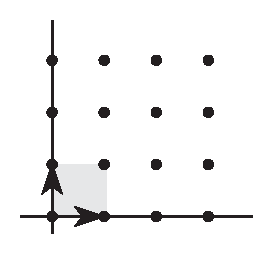
\includegraphics{lbasisa} 
   &
  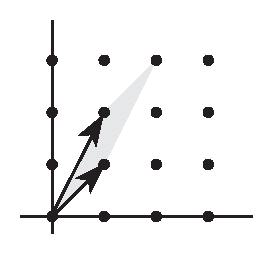
\includegraphics{lbasisb} \\
  (a) & (b)
 \end{tabular}
\end{center}
\caption{Two different bases for ${\protect\Z} \times {\protect\Z}$
     \label{Lattice:Basis:Fig}}
\end{figure}

A new geometric method of proving these results was given by {\Minkowski}
by his development of the \key{geometry of numbers}.  In this chapter
we follow {\Minkowski}'s lead and use these geometric techniques.  A
significant advantage of the geometric approach is the recent
development of (relatively) efficient algorithms for solving
multidimensional approximation problems like those mentioned above.
In addition to solving problems in diophantine approximation, these
algorithms can also be used to find relations between numbers and to
factor polynomials. 

\section{Lattice Fundamentals}
\label{Lattice:Fund:Sec}

The elements of $\mathbb{R}^{n}$ are $n$-tuples that for an additive group by 
component-wise addition. Multiplication by an element $a \in \mathbb{R}$ 
maps $\vec v = \langle v_1, v_2, \ldots, v_n \rangle \in \R^n$ to 
$a \vec v = \langle av_1, av_2, \ldots, a v_n \rangle$.

A \keyi{lattice} is a discrete subset of $\mathbb{R}^{n}$ that 
can be generated by $n$ linearly independent vectors: 
\begin{equation*}
{\cal L} = \{\, \lambda_{1} \vec b_{1} + \cdots + \lambda_{n} \vec b_{n} \mid
\lambda_{i} \in \Z \,\}.
\end{equation*}
We call $\{\vec b_{1}, \ldots, \vec b_{n}\}$ a {\em
basis}\index{lattice!  basis of} of the lattice ${\cal L}$.  As illustrated
in \figref{Lattice:Basis:Fig}, a lattice can have more than one basis.
In this case, the lattice is ${\cal L} = \Z \times \Z$.  In
\figref{Lattice:Basis:Fig}(a) we have shown the natural basis $\vec b_{1} =
(1, 0)$ and $\vec b_{2} = (0, 1)$, while \figref{Lattice:Basis:Fig}(b)
shows the alternative basis $\vec b_{1}' = (1, 2)$ and $\vec b_{2}' = (1, 1)$.
 
Each of these two figures includes a shaded parallelepiped defined by
the two basis vectors.  Each shaded region is called the
\keyi{fundamental domain} of the corresponding basis.  Repeated copies
of the fundamental domain \key{tessellate} $\mathbb{R}^{n}$.  As we shall see,
the volume of fundamental domain of a lattice is independent of the
basis used to define it.

The geometric properties of a lattice are induced by the definition
used for distance.  For all applications with which we are concerned,
the distance between two points is invariant under rigid translations
of the two points.  Thus the distance between the two points $\vec{x}$
and $\vec{y}$ is the length of the vector between them---that is, the
length of $\vec{x}-\vec{y}$.  When given suitable properties, a function
that maps vectors in $\Re^n$ into their length is called a \textbf{norm}.
We will only consider distance measures that are derived from norms.

\begin{definition}
A {\bf norm}\index{norm! of a lattice} on $\mathbb{R}^{n}$ is a map 
$d: \mathbb{R}^{n} \rightarrow \mathbb{R}$ such that 
\begin{enumerate}
\item $d(x) \ge 0$ for all $x \in \mathbb{R}^{n}$,
\item $d(x) = 0$ if and only if $x = 0$,
\item $d(\alpha x) = |\alpha| d(x)$, for $\alpha \in \mathbb{R}$,
\item $d(x+y) \le d(x) + d(y)$.
\end{enumerate}
\end{definition}

Each of these conditions has a natural geometric interpretation.  The
first two conditions say that the length of every vector other than
$(0, \ldots, 0)$ is positive.  The third says that if we scale the
entire space by a factor of $\alpha$ then the length of the vector
increases by a factor of $|\alpha|$.  The fourth condition is the
triangle inequality.

A frequently used collection of norms are the {\em
$p$-norms},\index{p-norm of a lattice@$p$-norm of a lattice} which are
denoted by $\|\;\|_{p}$.  If $x = (x_{1}, \ldots, x_{n})$ is a point
in $\mathbb{R}^{n}$, then $\|x\|_{p}$ is defined to be
\[
\|x\|_{p} = \sqrt[p]{|x_{1}|^{p} + |x_{2}|^{p} + \cdots + |x_{n}|^{p}}.
\]
Useful special cases of the $p$ norm are the $1$-norm of $x$,
$\|x\|_{1}$; the \keyi{Euclidean norm}, $\|x\| = \|x\|_{2}$; and the
maximum norm $\|x\|_{\infty}$.  The $1$-norm of $x$ is defined by
\[
\|x\|_{1} = |x_{1}| + |x_{2}| + \cdots + |x_{n}|,
\]
which is the ``Manhattan'' length of $x$.\index{Manhattan length} The
Euclidean distance function\index{Euclidean distance} is just the $2$-norm:
\[
\|x\|_{2} = \sqrt{|x_{1}|^{2} + |x_{2}|^{2} + \cdots + |x_{n}|^{2}}.
\]
The \keyi{maximum norm} is the limit of $\|x\|_{p}$ as $p$ goes to
infinity:
\[
\|x\|_{\infty} = \max (|x_{1}|, \ldots, |x_{n}|).
\]
All of the $p$-norms generate the same topology on $\mathbb{R}^{n}$.
\addsymbol{$\|\vec{v}\|_p$}{$p$ norm of a vector}
\addsymbol{$\|\vec{v}\|$}{$2$ norm of a vector, Euclidean distance}
\addsymbol{$|\vec{v}|$}{$\infty$ norm of a vector, sum of absolute
values of its components}

The fact that the $p$-norms are norms follows from the \keyi{Minkowski
inequality} \cite[pages 115--117]{Minkowski2018-iz}:

\begin{proposition}[{\Minkowski}]
If $x_1, \ldots, x_n$ and $y_1, \ldots, y_n$ are non-nega\-tive real
numbers, then for all $p \ge 1$
\[
\left(|x_1 + y_1|^p + \cdots + |x_n + y_n|^p\right)^{1/p} \le 
\left(x_1^p + \cdots + x_n^p\right)^{1/p} + 
\left(y_1^p + \cdots + y_n^p\right)^{1/p}.
\]
\end{proposition}

\noindent
A proof of this proposition can be found in \cite{Hardy1952-ad}.\Marginpar{Include the proof here.}

Determining whether a set of points is a lattice can be quite
difficult, if the set is not specified in terms of set of basis
vectors.  In this situation the following proposition is quite useful.
For a proof see {\Cassels} \cite[page 78]{Cassels2012-kd}.

\begin{proposition} \label{Lattice:Condition:Prop}
A necessary and sufficient condition that a set of points ${\cal L} \subset
\mathbb{R}^n$ be a lattice is that the set satisfy:
\begin{itemize}
\item ${\cal L}$ is closed under component-wise addition,
\item ${\cal L}$ contains $n$ linearly independent points,
\item There exists a constant $\eta> 0$ such that if $(x_1, \ldots,
x_n) \in {\cal L}$ and
\[
\sqrt{x_1^2 + \cdots + x_n^2} < \eta,
\]
then $x_1 = x_2 = \cdots = x_n = 0$.
\end{itemize}
\end{proposition}

The first two conditions ensure that there is a basis for the points
of ${\cal L}$.  The third condition states that there is a neighborhood of
the origin that contains only one point.  This ensures that all the
points of ${\cal L}$ are separated and thus the basis is a $\Z$ lattice.

\paragraph{Fundamental Domains}

\begin{figure}
\begin {center}
 \begin {tabular}{cc}
   \begin{picture}(150, 62)
     \put(0,0){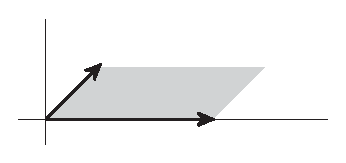
\includegraphics{FundDoma}}
     \put(85,0){$\vec{a}$}
     \put(30,42){$\vec{b}$}
   \end{picture}
  & 
   \begin{picture}(150, 62)
     \put(0,0){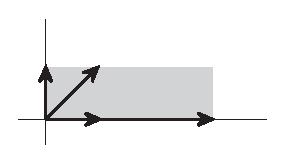
\includegraphics{FundDomb}}
     \put(100,0){$\vec{a}$}
     \put(40,42){$\vec{b}$}
     \put(40,0){$\vec{b}_{\parallel}$}
     \put(3,42){$\vec{b}_{\perp}$}
   \end{picture} \\
   (a) & (b) 
 \end{tabular}
\end{center}
\caption{Computing the Area of a
Parallelogram\label{Lat:Parallel:Fig}}
\end{figure}

The volume of the fundamental domain is an important property of a
lattice.  As we shall show, it does not depend on the basis, but is an
invariant of the lattice.  If the basis vectors are orthogonal then
the volume of fundamental domain is just the product of the lengths of
the vectors.  Recall that two vectors $\vec{a}$ and $\vec{b}$ are
orthogonal if and only if their {\em dot product}\index{dot product!of two
vectors} vanishes
\[
\vec{a} \cdot \vec{b} = a_1 b_1 + \cdots + a_n b_n = 0.
\]
To compute the volume of a general parallelepiped we modify
the basis vectors in such a way that the volume is left unchanged, but
the new vectors are orthogonal.  This is illustrated in
\figref{Lat:Parallel:Fig}. 
\addsymbol{$\vec{a}\cdot\vec{b}$}{Dot product of $\vec{a}$ and
$\vec{b}$, $a_1 b_1 + \cdots + a_n b_n$}

The area of the parallelogram bounded by the vectors $\vec{a}$ and
$\vec{b}$ is the same as that of the rectangle in
\figref{Lat:Parallel:Fig}(b).  In \figref{Lat:Parallel:Fig}(b), we
have decomposed $\vec{b}$ into the sum of two orthogonal vectors
$\vec{b}_{\perp}$ and $\vec{b}_{\parallel}$.  $\vec{b}_{\parallel}$ is
the portion of $\vec{b}$ that is parallel to $\vec{a}$ and does not
contribute to the area of the parallelogram.  Thus, the area delimited
by $\vec{b}_{\perp}$ and $\vec{a}$ is the same as that
delimited by $\vec{a}$ and $\vec{b}$.  The magnitude of
$\vec{b}_{\parallel}$ is $\vec{b} \cdot \vec{a}$, so 
\[
\vec{b}_{\perp} = \vec{b} - \frac{\vec{b} \cdot \vec{a}}{\|\vec{a}\|} \,
\frac{\vec{a}}{\|\vec{a}\|} = 
\vec{b} - \frac{\vec{b} \cdot \vec{a}}{\vec{a} \cdot \vec{a}}\,
\vec{a}\;,
\]
where the second factor is the unit vector parallel to $\vec{a}$.
So, if we denote by $\vec{b}^{\ast} = \vec{b}_{\perp}$ and
$\vec{a}^{\ast} = \vec{a}$ the orthogonalization of $\vec{a}$ and
$\vec{b}$ we have
\[
\left(\begin{array}{c} \vec{a} \\ \vec{b} \end{array}\right)
= 
\left(\begin{array}{cc} 1 & 0 \\ 
\frac{\vec{b} \cdot \vec{a}}{\vec{a} \cdot \vec{a}} & 1 \end{array}\right)
\cdot
\left(\begin{array}{c} \vec{a}^{\ast} \\ \vec{b}^\ast \end{array}
\right)
\]
More generally, we can orthogonalize the vectors $\vec{a}_1, \ldots,
\vec{a}_n$ as follows
\[
\begin{array}{l} \vec{a}_1 = \vec{a}^{\ast}_1 \\ \vec{a}_2 \\ \vec{a}_3 \\ \vdots \\ \vec{a}_n \end{array}
\Rightarrow
\begin{array}{l} \vec{a}^{\ast}_1 \\ 
   \vec{a}_2 -\mu_{21} \vec{a}^{\ast}_1 = \vec{a}^{\ast}_2 \\
   \vec{a}_3 - \mu_{31} \vec{a}^{\ast}_1\\ \vdots \\ \vec{a}_n -\mu_{n1} \vec{a}^{\ast}_1
\end{array}
\Rightarrow
\begin{array}{l} \vec{a}^{\ast}_1 \\ 
   \vec{a}^{\ast}_2 \\ 
   (\vec{a}_3 - \mu_{31} \vec{a}^{\ast}_1) - \mu_{32}\vec{a}^{\ast}_2 = \vec{a}^{\ast}_3 \\ 
   \vdots \\ (\vec{a}_n -\mu_{n1} \vec{a}^{\ast}_1)  - \mu_{n2}\vec{a}^{\ast}_2 
\end{array}
\Rightarrow
\cdots
\]
where the $\vec{a}^{\ast}_i$ are elements of the final orthogonal
basis.  The number $\mu_{ij}$ is the magnitude of the component of
$\vec{a}_i$ parallel to $\vec{a}^{\ast}_j$.

The computation of the orthogonal basis is initiated by setting
$\vec{a}^{\ast}_1 = \vec{a}_1$.  At the $i$-th step, each of the
remaining vectors (numbered $i+1$ through $n$) is modified so as to be
orthogonal to $\vec{a}^{\ast}_i$.  This process is called the
(modified) {\em Gram-Schmidt orthogonalization
process}.\index{Gram-Schmidt algorithm} The following code makes this
procedure precise.

\begindsacode
GramSchmidt ($\vec{a}_1, \ldots, \vec{a}_n$) := $\{$\\
\>loo\=p for $i = 1, \ldots, n$  do \{ \\
\>\> $\vec{a}^{\ast}_i \leftarrow \vec{a}_i$; \\
\>\> \} \\
\>loop for $i = 1, \ldots, n$  do \{ \\
\>\> loo\=p for $j = i+1, \ldots, n$ do \{\\
\>\> \> $\vec{a}^{\ast}_j \leftarrow \vec{a}^{\ast}_j 
     - (\vec{a}^{\ast}_j \cdot \vec{a}^{\ast}_i)/(\vec{a}^{\ast}_i \cdot \vec{a}^{\ast}_i) \vec{a}^{\ast}_i$; \\
\>\>\> \} \\
\>\> \} \\
\>return ($\vec{a}^{\ast}_1, \ldots, \vec{a}^{\ast}_n$); \\
\>$\}$
\enddsacode

If the vectors $\vec{a}_1, \ldots, \vec{a}_n$ are arranged to form a
matrix $A$, we see that the Gram-Schmidt process factors $A$ into two
matrices as follows:
\begin{equation} \label{Gram:Schmidt:Eq}
\begin{aligned}
\left(
 \begin{array}{c}
   \vec{a}_1 \\ \vec{a}_2 \\ \vec{a}_3 \\ \vdots \\ \vec{a}_n
 \end{array}
\right)
 & = 
\left(
 \begin{array}{cccccc}
   1 & 0 & 0 & \cdots & 0 & 0 \\ 
   \mu_{21} & 1 & 0 & \cdots & 0 & 0 \\ 
   \mu_{31} & \mu_{32} & 1 & \cdots & 0 & 0 \\
   \vdots & & \vdots & & & \vdots \\ 
   \mu_{n1} & \mu_{n2} & \mu_{n3} & \cdots & \mu_{n,n-1} & 1
 \end{array}
\right)
\cdot 
\left(
 \begin{array}{c}
   \vec{a}^{\ast}_1 \\ \vec{a}^{\ast}_2 \\ \vec{a}^{\ast}_3 \\ 
   \vdots \\ \vec{a}^{\ast}_n
 \end{array}
\right) \\
 & = Q \cdot A^{\ast}
\end{aligned}
\end{equation}
The determinant of $A^{\ast}$ is the product of the lengths of the
(orthogonal) basis vectors $\vec{a}^{\ast}_i$ as we show in
\propref{Hadamard:Ineq:Prop}.
Taking the determinant of the previous equation, we have
\[
\begin{aligned}
  \det A & = (\det Q) (\det A^{\ast}) \\
    & = \|\vec{a}^{\ast}_1\| \cdots \|\vec{a}^{\ast}_n\| = \det {\cal L},
\end{aligned}
\]
since the determinant of $Q$ is $1$.
Thus the volume of the fundamental domain of a lattice is identical to
the determinant of the lattice.  This is stated formally in
\propref{Parallelepiped:Vol:Prop}.  

\begin{proposition}\label{Parallelepiped:Vol:Prop}
The volume of the parallelepiped $\Delta$ bounded by the vectors
$\{\vec{a}_{1}, \ldots, \vec{a}_{n}\}$ is
\[
\vol(\Delta) = \left|
\begin{array}{ccc}
a_{11} & \cdots & a_{1n} \\
\vdots &   & \vdots \\
a_{n1} & \cdots & a_{nn}
\end{array}
\right|,
\]
where $\vec{a}_{i} = (a_{i1}, a_{i2}, \ldots, a_{in})$.
\end{proposition}

\smallskip
The above discussion used a special case of the following proposition due to
{\Hadamard} \cite{Hadamard1893-xq}. 

\begin{proposition}[Hadamard] \label{Hadamard:Ineq:Prop}
Let $\vec a_{i} = (a_{i1}, \ldots, a_{in})$ be $n$ vectors whose
components lie in $\C$, then
\[
A = \det\left( \begin{array}{c} \vec{a}_1 \\ \cdots \\ \vec{a}_n \end{array}\right)
 = \left|
 \begin{array}{cccc}
a_{11} & \cdots & a_{1n} \\
\vdots &  & \vdots \\
a_{n1} & \cdots & a_{nn} 
\end{array}
\right| \le
\prod_{1 \le i \le n} \|\vec a_{i} \|.
\]
Equality is achieved if and only if the rows of the determinant are
orthogonal. 
\end{proposition}

Intuitively, this theorem can be justified as follows.  By
\propref{Parallelepiped:Vol:Prop} the determinant is the volume of the
parallelepiped with edges $\vec{a}_i$.  This volume is maximized when
the edge vectors are orthogonal (all the corners of the
parallelepiped are right angles).  \Eg, a rectangle has the largest
area of all parallelograms with specified edge lengths.  In the
orthogonal case the volume of the parallelepiped is the product on
the right.  

This argument is circular since we used Hadamard's proposition to show
that the volume of a parallelepiped was the determinant of the
appropriate matrix.  The following proof does not have this problem. 

\begin{proof} 
We proceed by contradiction.
Without loss of generality, we can assume each vector $\vec{a}_i$  has
length $1$.  Assume the $\vec{a}_i$ are chosen so as to 
maximize $A$.  Since the identity matrix satisfies all the conditions
of the proposition and has determinant $1$, so
$A > 1$.  Now assume that the first two rows of $A$ are not
orthogonal.  We shall show that $A$ cannot then be maximal.
\addsymbol{$\overline{\protect\vphantom{b}a}$}{Complex conjugate of $a$}

We have
\[
C = \sum_{1 \le j \le n}\overline{\vphantom{b}a_{1j}} a_{2j},
\]
where the overbar in $\overline{\vphantom{b}a_{1j}}$ indicates the
\keyi{complex conjugate}. 
Construct a new matrix whose second row is orthogonal to the first,
but which is otherwise unchanged, \ie, $a'_{2j} = \lambda a_{1j} + \mu
a_{2j}$ such that
\[
\sum_{1 \le j \le n} a'_{2j} \overline{\vphantom{b}a_{1j}} = 0
\qquad\mbox{and}\qquad
\sum_{1 \le j \le n} |a'_{2j}|^2 = 1.
\]
Denote the determinant of this new matrix by $A' = \mu A$.

Replacing $a'_{2j}$ by $\lambda a_{1j} + \mu a_{2j}$ in the first
summation gives $\lambda + \mu C = 0$.  Proceeding similarly with the
second summation:
\[
\begin{aligned}
\sum_{1 \le j \le n} |a'_{2j}|^2  & = 
\sum_{1 \le j \le n} (\lambda a_{1j} + \mu a_{2j}) 
  (\overline{\lambda} \overline{\vphantom{b}a_{1j}} + \overline{\vphantom{b}\mu}
\overline{\vphantom{b}a_{2j}})  \\
  & = |\lambda|^2 + \mu \overline{\lambda} C 
        + \lambda \overline{\vphantom{b}\mu}\overline{C} + |\mu|^2 = 1.
\end{aligned}
\]
Using $\lambda + \mu C = 0$ to eliminate $\lambda$ we have 
$|\mu|^2 ( 1 - |C|^2) = 1$, or $|\mu|^2 > 1$, which contradicts the
claim that $A$ was maximal.  Thus the matrix achieves its maximal
value when the rows are orthogonal.

Since we now know that the rows are orthogonal we can compute the
determinant quite easily.  The product of the matrix with the complex
conjugate of its transpose is
\[
\left(
 \begin{array}{cccc}
a_{11} & \cdots & a_{1n} \\
\vdots &  & \vdots \\
a_{n1} & \cdots & a_{nn} 
\end{array}
\right)
\cdot
\left(
 \begin{array}{cccc}
\overline{\vphantom{b}a_{11}} & \cdots & \overline{\vphantom{b}a_{n1}} \\
\vdots &  & \vdots \\
\overline{\vphantom{b}a_{1n}} & \cdots & \overline{\vphantom{b}a_{nn}} 
\end{array}
\right) =
\left(\sum_{1 \le k \le n} a_{ik} \overline{\vphantom{b}a_{jk}}\right)_{i,j}
= {\bf 1}.
\]
So $A = 1$, as desired.
\end{proof}


\begin{proposition}
The volume of the fundamental domain of a lattice is independent of
the basis used to compute it.
\end{proposition}

\begin{proof}
Let ${\cal L}$ be the lattice generated by the vectors $\{\vec{b}_i\}$ and
let $\{\vec{b}'_i\}$ be a different basis for ${\cal L}$.  Since each of
the vectors $\vec{b}'_i$ is an element of ${\cal L}$, each $\vec{b}'_i$ can
be represented as a linear combination of the $\vec{b}_i$:
\[
\vec b_{i}' = a_{i1} \vec b_{1} + a_{i2} \vec b_{2} + \cdots + a_{in} \vec b_{n},
\qquad 1 \le i \le n,
\]
where the $a_{ij}$ are elements of $\Z$.  Similarly, there exist
$a'_{ij}$ such that
\[
\vec b_{j} = a_{j1}' \vec b_{1}' + a_{j2}' \vec b_{2}' + \cdots + a_{jn}'
\vec b_{n}',
\qquad 1 \le j \le n.
\]
Define the transformation matrices $A =
(a_{ij})$ and $A' = (a_{ij}')$.
Composing these two transformations leaves a basis unchanged, so $AA'
= A' A = I$.  Thus the volume of the fundamental region of a lattice is 
independent of the basis chosen.  
It is denoted by $\det({\cal L})$.
\end{proof}

\paragraph{Sub-Lattices}

A subset of a lattice that is also a lattice is called a
\keyi{sub-lattice}.  Let $\vec{a}_1, \ldots, \vec{a}_n$ be linearly
independent elements of the lattice ${\cal L}$.  They are the basis of
a second lattice ${\cal M}$, which is a sub-lattice of ${\cal L}$.
Since the $\vec{a}_i$ are elements of ${\cal L}$ they can be written
as
\begin{equation} \label{SubLatt:a:Eq}
\vec{a}_i = \sum_j v_{ij} \vec{b}_j.
\end{equation}

Taking the determinant of these equations gives
\[
\det {\cal M} = \det (v_{ij}) \cdot \det {\cal L}.
\]
The {\em index}\index{index!of a sub-lattice} of ${\cal L}$ is defined
to be 
\begin{equation} \label{Latt:Index:Eq}
I = \det (v_{ij}) = \frac{\det {\cal M}}{\det {\cal L}}.
\end{equation}
The index of a sub-lattice is independent of the choice of bases.
The linear equations \eqnref{SubLatt:a:Eq} can be solved for the
$\vec{b}_j$ as linear combinations of the $\vec{a}_i$.  The
denominators of these coefficients is $\det(v_{ij}) = i$.  So we have
\[
I \vec{b}_j = \sum_i w_{ij} \vec{a}_{i},
\]
where the $w_{ij}$ are rational integers.  Thus, $I {\cal L} \subseteq
{\cal M} \subseteq {\cal L}$.

The following proposition shows that a basis can be found for the
sub-lattice ${\cal M}$ with a very specific structure.

\begin{proposition} \label{SubLattice:Basis:Prop}
Let ${\cal M}$ be a sub-lattice of ${\cal L} = (\vec{b}_1, \ldots,
\vec{b}_n)$.  Then a basis, $\vec{a}_1, \ldots, \vec{a}_n$ for ${\cal
M}$ can be found such that 
\begin{equation} \label{SubLatt:Basis:Eq}
\begin{aligned}
\vec{a}_1 & = v_{11} \vec{b}_1, \\
\vec{a}_2 & = v_{21} \vec{b}_1 + v_{22} \vec{b}_2, \\
  & \vdots \\
\vec{a}_n & = v_{n1} \vec{b}_1 + \cdots + v_{n2} \vec{b}_n,
\end{aligned}
\end{equation}
where the $v_{ij}$ are integers and $v_{ii}$ are positive.
Conversely, for every basis $\vec{a}_1, \ldots, \vec{a}_n$ of ${\cal
M}$ there exists a basis $\vec{b}_1, \ldots, \vec{b}_n$ such that
\eqnref{SubLatt:Basis:Eq} holds with integer $v_{ij}$.
\end{proposition}

\begin{proof}
We start with the forward direction, with a basis $\vec{b}_1, \ldots,
\vec{b}_n$ of ${\cal L}$.  Since ${\cal M}$ is a sub-lattice of ${\cal
L}$, every element of ${\cal M}$ can be uniquely written as
\[
c_{i1} \vec{b}_1 + c_{i2} \vec{b}_2 + \cdots c_{in} \vec{b}_n,
\]
where the $c_{ij}$ are integers.  Of all these elements we choose an
element with smallest positive $c_n$.  Denote this element by 
\[
\vec{a}_n = c_{1n} \vec{b}_1 + \cdots c_{nn} \vec{b}_n.
\]

We claim that $c_{nn}$ divides the
coefficient of $\vec{b}_n$ of every element of ${\cal M}$.  If this
were not the case there would be a
\[
\vec{a}^{\ast} = c_1^{\ast} \vec{b}_1 + \cdots c_n^{\ast} \vec{b}_n
\]
such that the greatest common divisor of $c_n^{\ast}$ and $c_{nn}$,
$d$ lies between $0$ and $c_{nn}$.  But then there would be $A$ and
$B$ such that $A c^{\ast}_n + B c_{nn} = d$.  Thus,
\[
A \vec{a}_n + B \vec{a}^{\ast} = c^{\ast\ast}_1 \vec{b}_1 + \cdots + d
\vec{b}_n,
\]
whose coefficient of $\vec{b}_n$ is not divisible by $c_{nn}$.  

Continuing this process for the coefficient of $\vec{b}_{n-1}$ we have
\[
\begin{aligned}
\vec{a}_1 & = c_{11} \vec{b}_1,  \\
\vec{a}_2 & = c_{21} \vec{b}_1 + c_{22} \vec{b}_2,  \\
   & \vdots \\
\vec{a}_n & = c_{n1} \vec{b}_1 + \cdots + c_{nn} \vec{b}_n,  
\end{aligned}
\]
and the $c_{ii}$ are as small as possible.  These vectors are 
linearly independent and every element of ${\cal M}$ is a linear
combination of the $\vec{a}_i$ by the reasoning above. 

In the converse direction, since $I {\cal L}$ is contained in ${\cal
M}$, we have
\[
\begin{aligned}
I \vec{b}_1 & = v_{11} \vec{a}_1,  \\
I \vec{b}_2 & = v_{21} \vec{a}_1 + v_{22} \vec{a}_2,  \\
   & \vdots \\
I \vec{b}_n & = v_{n1} \vec{a}_1 + \cdots + v_{nn} \vec{a}_n,  
\end{aligned}
\]
where the $v_{ij}$ are integers.  The system can be solved to produce
\[
\begin{aligned}
\vec{a}_1 & = w_{11} \vec{b}_1,  \\
\vec{a}_2 & = w_{21} \vec{b}_1 + w_{22} \vec{b}_2,  \\
   & \vdots \\
\vec{a}_n & = w_{n1} \vec{b}_1 + \cdots + w_{nn} \vec{b}_n,  
\end{aligned}
\]
where the the $w_{ij}$ may be rational numbers.  Since the $\vec{b}_i$
are a basis of ${\cal L}$ and the $\vec{a}_i$ are elements of ${\cal
L}$ the the $w_{ij}$ are actually integers.
\end{proof}

Since both a sub-lattice and a lattice are additive groups, we can
form the quotient of ${\cal L}/{\cal M}$.  The sub-lattice has a
larger fundamental domain than that of ${\cal L}$.  We can think of
the fundamental domain of ${\cal L}$ tiling the fundamental domain of
${\cal M}$.    This suggests that the number of elements of ${\cal
L}/{\cal M}$ is equal to the index of ${\cal M}$ in ${\cal L}$.  This
is the case as is shown in the proof of the following proposition.

\begin{proposition} \label{SubLattice:Index:Prop}
Let ${\cal M}$ be a sub-lattice of ${\cal L}$.  Then the number of
elements of ${\cal L}/{\cal M}$ is equal to the index of ${\cal M}$ in
${\cal L}$, $\det {\cal M}/\det {\cal L}$.
\end{proposition}

\begin{proof}
By \propref{SubLattice:Basis:Prop}, ${\cal M}$ has a basis that can be
represented in terms of the basis vectors of ${\cal L}$ as in
\eqnref{SubLatt:Basis:Eq}.  By reduction with respect to this basis,
an element of ${\cal L}/{\cal M}$ is of the form
\[
u_1 \vec{b}_1 + u_2 \vec{b}_2 + \cdots + u_n \vec{b}_n,
\]
where $0 \le u_i < v_{ii}$.  Therefore, there are 
\[
v_{11} v_{22} \cdots v_{nn}
\]
elements in ${\cal L}/{\cal M}$.  But this is the index of ${\cal M}$
in ${\cal L}$.
\end{proof}

\section{Minkowski Convex Body Theorem}
\index{Minkowski convex body theorem|(}

Intuitively, a convex body in $\mathbb{R}^{n}$ is region of $\mathbb{R}^{n}$ that has
no holes or surface depressions.  Let $C$ be an $n$-dimensional
bounded subset of $\mathbb{R}^n$.  We call such a set a {\em body}.  $C$ is
said to be {\em convex}\index{convex body} if, for every pair of
points $x$, $y$ in $C$ and real number $\mu \in [0, 1]$, $\mu x + (1 -
\mu) y$ is also in $C$.  A convex body $C$ is {\em
symmetric}\index{convex body!symmetric} if, for every $x \in C$, $-x$
is also in $C$.  Thus a symmetric \key{convex body} includes the origin.

\begin{proposition}[{\Minkowski}]
Let $C$ be a symmetric convex body in $\mathbb{R}^{n}$, ${\cal L}$ a lattice in
$\mathbb{R}^{n}$.  If either
\[
\vol C > 2^n \det {\cal L}
\]
or 
\[
\vol C = 2^n \det {\cal L}, \quad \mbox{and $C$ is compact}
\]
then $C$ contains a non-zero element of ${\cal L}$.
\label{Minkowski:Convex:Prop}
\end{proposition}

\begin{proof}
Let $\Delta$ be a fundamental domain of ${\cal L}$ with respect to some basis,
$\vol \Delta = \det {\cal L}$.  Let $C' = \frac{1}{2}C$, \ie\ each point has
all of its coordinates multiplied by $\frac{1}{2}$, so 
\[
\vol C' = \frac{1}{2^{n}} \vol C.
\]
Initially, assume $\vol C' > \vol \Delta$.  $C'$ only intersects a
finite number of fundamental domains of ${\cal L}$ (since $C'$ is finite and
thus its closure is compact).  Denote these regions by
$\ell_{1}+\Delta, \ldots, \ell_{r}+\Delta$.  The volume of $C'$ is 
\begin{equation}
\vol(C') = \vol(C' \cap (\ell_{1}+\Delta)) + \cdots +
\vol(C' \cap (\ell_{r}+\Delta)).
\label{Mink:Vol:Eq}
\end{equation}
The volume of $C' \cap (\ell + \Delta)$ is the same as $(C' - \ell) \cap
\Delta$.  Instead of shifting $\Delta$ to intersect $C'$, we shift $C'$
to intersect $\Delta$:
\[
\vol C' = \vol((C' - \ell_{1}) \cap \Delta) + \cdots +
\vol((C' - \ell_{r}) \cap \Delta)
> \vol(\Delta).
\]
There are at least two sets $C' - \ell_{i}$ and $C' -\ell_{i}$ that are
not disjoint.  So there are $x', y' \in C'$ such that $x' - \ell_{i} = y' -
\ell_{j}$.  Consider the lattice point 
\[
\ell_{j} - \ell_{i} = y' - x' = \frac{1}{2}y - \frac{1}{2}x.
\]
Since $x$ and $y$ are in $C$, by convexity and symmetry of $C$, the
lattice point $\ell_{j} - \ell_{i}$ is in $C$.

Now assume that $C$ is compact and  $\vol C' = \vol \Delta$.  In this case we enlarge $C$
slightly so that the previous case applies.  If $m$ is some positive number
then
\[
\vol\left(\left(1+\frac{1}{m}\right)C\right) = \left[1+\frac{1}{m}\right]^{n} \vol(C)
> 2^{n} \vol(\Delta).
\]
By the previous discussion $(1+\frac{1}{m})C \cap {\cal L} \not= \{0\}$, \ie\
it contains a non-zero element.  As $m$ goes to infinity
\[
\left(1+\frac{1}{m}\right)C \supseteq \left(1+\frac{1}{m+1}\right)C 
\supseteq \left(1+\frac{1}{m+2}\right)C \supseteq \cdots.
\]
Each of $(1+\frac{1}{m})C \cap {\cal L} -\{0\}$ is non-empty.  Eventually they
must all be the same since the lattice ${\cal L}$ is discrete.  Since $C$ is compact
\[
\bigcap_{m>0} \left(1+ \frac{1}{m}\right) C = C,
\]
$C \cap {\cal L} - \{0\}$ must also be non-empty.
\end{proof}

\paragraph{Dirichlet's Theorems}

{\Minkowski}'s theorem yields easy proofs of Propositions
\ref{Dirichlet:Multiple:Prop} and \ref{Dirichlet:Mutual:Prop}.  
To prove \propref{Dirichlet:Multiple:Prop} for arbitrary $n$, we use
the lattice generated by:
\[
\left(\begin {array}{c} 
  \vec{b}_0 \\ \vec{b}_1 \\ \vec{b}_2 \\ \vdots \\ \vec{b}_n 
\end{array}\right)
=
\left(\begin {array}{ccccc}
  \epsilon^n & \alpha_1/\epsilon & \alpha_2/\epsilon & 
    \ldots & \alpha_n/\epsilon \\
  0 & 1/\epsilon & 0 & \ldots & 0 \\
  0 & 0 & 1/\epsilon & \ldots & 0 \\
  \vdots  & & \vdots & &\vdots \\
  0 & 0 & 0 & \ldots & 1/\epsilon
\end{array}
\right).
\]
The volume of the fundamental domain of this lattice is clearly 1.
The $n+1$ dimensional cube, $|x_i| \le 1$, is a convex body with
volume $2^{n+1}$ satisfying the convex body theorem.

For the point $q \vec{b}_0 - p_1 \vec{b}_1 - \cdots - p_n \vec{b}_n$
to lie in the cube the following inequalities must hold.
\[
\begin{aligned}
|q\epsilon^n| &\le 1, \qquad \Longrightarrow\qquad 
    \frac{1}{|q|^{1/n}} \ge \epsilon, \\
|p_i - q \alpha_i| &\le \epsilon.
\end{aligned}
\]
Combining these two inequalities gives 
\propref{Dirichlet:Multiple:Prop}.

To prove \propref{Dirichlet:Mutual:Prop} we use the lattice
\begin{equation} \label{Dirichlet:Lattice:Eq}
\left(
\begin{array}{c}
  \vec{b}_0 \\ \vec{b}_1 \\ \vec{b}_2 \\ \vdots \\ \vec{b}_n
\end{array}\right) =
\left(\begin{array}{cccccc}
1/\epsilon &  0 & 0 & \ldots & 0 \\
\alpha_1/\epsilon & \epsilon^{1/n} & 0 & \ldots & 0 \\
\alpha_2/\epsilon & 0 & \epsilon^{1/n} & \ldots & 0  \\
\vdots  & & \vdots & & \vdots \\
\alpha_n/\epsilon & 0 & 0 & \ldots & \epsilon^{1/n}
\end{array}\right).
\end{equation}
Again by the convex body theorem, there exist integers $p_0, p_1,
\ldots, p_n$ such that $p_0 \vec{b}_0 + p_1 \vec{b}_1 + \cdots + p_n
\vec{b}_n$ lies within the cube $|x_i| \le 1$.  Examining the
components of this vector we see that
\[
\left| p_0 + p_1 \alpha_1 + \cdots p_n \alpha_n\right| \le \epsilon,
\]
and 
\[
\left|p_i\right| \le \epsilon^{-1/n}, \quad \mbox{for $1 \le i \le n$}
\]
as desired.
\index{Minkowski convex body theorem|)}

\section{Reduced Bases}
\label{Lovasz:Basis:Sec}

The previous sections of this chapter have illustrated how many
problems can be phrased in terms of finding short vectors in a
lattice.  In this section, we look at the algorithmic problem of
finding short vectors.  If the basis vectors of a lattice are
orthogonal, then the shortest vector in the lattice will be one
of the basis vectors.  Not all lattices have orthogonal bases, but
this provides one approach to the short vector problem.  We seek a
sequence of unimodular transformations\index{unimodular matrix} that
yields a new set of basis vectors that are as close to orthogonal as
possible.  Then the smallest vector of this ``nearly orthogonal''
basis will be short. 

Let $\vec{b}_1, \ldots, \vec{b}_n$ be the basis for a lattice ${\cal L}$, and
let 
\[
\vec{v} = \lambda_1 \vec{b}_1 + \cdots + \lambda_n \vec{b}_n,
\]
be a short vector in ${\cal L}$.  By Cramer's rule and
\propref{Hadamard:Ineq:Prop}, we can bound $\lambda_i$ by 
\[
\begin{aligned}
  |\lambda_i| & = \left|\frac{\det(\vec{b}_1, \ldots, \vec{b}_{i-1},
\vec{v}, \vec{b}_{i+1}, \ldots, \vec{b}_n)}{\det(\vec{b}_1, \ldots,
\vec{b}_n)} \right|, \\
  & \le \frac{\|\vec{b}_1\| \cdots \|\vec{b}_{i-1}\|\, \|\vec{v}\|\,
\|\vec{b}_{i+1}\| \cdots \|\vec{b}_n\|}{\left|\det(\vec{b}_1, \ldots,
\vec{b}_n)\right| }.
\end{aligned}
\]
Assuming $\vec{v}$ is no larger than the smallest basis vector, we
have
\[
|\lambda_i | \le  \frac{\|\vec{b}_1\|
\cdots\|\vec{b}_n\|}{\left|\det(\vec{b}_1, \ldots, \vec{b}_n)\right|} = \delta,
\]
where we call $\delta$ the \keyi{orthogonality defect} of the basis
$\vec{b}_1, \ldots, \vec{b}_n$.

So the short vectors of a lattice are those of the form
\[
\lambda_1 \vec{b}_1 + \cdots + \lambda_n \vec{b}_n , \quad |\lambda_i|
\le \delta.
\]
When $\vec{b}_1, \ldots, \vec{b}_n$ are orthogonal, $\delta = 1$ and
there are only $3^n$ candidates.  However, by the triangle inequality,
the shortest vector must be one of the basis vectors.  We state this
formally as,

\begin{proposition} \label{Lat:Min:Vector:Prop}
Let $\vec{b}_1, \ldots, \vec{b}_n$ be a basis for the lattice ${\cal
L}$ and let $\vec{b}^{\ast}_1, \ldots, \vec{b}^{\ast}_n$ be its
Gram-Schmidt orthogonalization.\index{Gram-Schmidt algorithm} For
every non-zero vector $\vec{v} \in {\cal L}$
\[
\|\vec{v}\| \ge \min \{ \|\vec{b}^{\ast}_1\|, \ldots,
\|\vec{b}^{\ast}_n\| \}
\]
\end{proposition}

For non-orthogonal bases $\delta$ can be substantially larger, and the
shortest vector may be other than a basis vector.  In this case, all
$(2\lfloor \delta\rfloor + 1)^n$ possibilities must be examined.
{\Hermite} \cite{Hermite1950-ae} showed that for every lattice there
exists a basis $\vec{b}_i$ such that
\[
1 \le \frac{\|\vec{b}_1\| \, \|\vec{b}_2\| \cdots \|\vec{b}_n\|}{\det {\cal L}}
   \le c_n,
\]
where $c_n$ depends only on the dimension of the lattice.  For
sufficiently large values of $n$, the best known value of $c_n$ is
\[
c_n = 1.43 (0.97 n)^n n^{1/4} = 2^{O(n\log n)}.
\]

We are not able to produce a basis with such a small orthogonality
defect in polynomial time.  Instead, we will produce an orthogonality
defect of approximately $2^{n^2}$.  This gives a basis vector no
worse than a factor of $2^n$ larger than the shortest vector.

\medskip
The basic technique of the {\Lovasz} basis algorithm is quite simple.
The original basis is transformed into one that is as close as
possible to an orthogonal basis.  Then pairs of basis vectors are
interchanged to enforce a relative size ordering on the basis, and the
basis is ``orthogonalized'' again.  When this process terminates (it
is not obvious that it does), the remaining basis has the desired
properties.

The first step, the reduction of the basis to near orthogonality is
called \keyi{weak reduction} and is
quite easy to explain.  Using the \key{Gram-Schmidt algorithm}, the
relationship between the basis vectors and the orthogonalization of
the basis can be written as:
\begin{equation} \label{Lat:WeakB:Eq}
\left(
 \begin{array}{c} \vec{b}_1 \\ \vdots \\ \vec{b}_n \end{array}
\right)
= B = Q B^{\ast} = 
Q \left(
 \begin{array}{c} \vec{b}^{\ast}_1 \\ \vdots \\ \vec{b}^{\ast}_n \end{array}
\right),
\end{equation}
where $Q$ is lower triangular with $1$'s on the diagonal.  The matrix
$Q$ does not necessarily contain integer entries and may not be
unimodular,\index{unimodular matrix} so while the rows of $B^{\ast}$
are orthogonal, they do not generate ${\cal L}$.

The size of the lower triangular elements of $Q$ is a measure of how
far the basis $\vec{b}_i$ is from orthogonal.  By a sequence of
integer row operations, we can produce a new basis $B'$ from $B$ such
that $B' = \bar{Q} B^{\ast}$ and where the lower triangular elements of
$\bar{Q}$ have absolute value less than $1/2$.  The rows of $B'$ are
the {\em weak reduction} of the basis $\vec{b}_i$.  A basis is said
to be weakly reduced if $B = QB^{\ast}$, where the lower triangular
elements of $Q$ have absolute value less than $1/2$.

A basis is weakly reduced by starting at the bottom of the $Q$ matrix
and working upwards and performing row operations to reduce the size
of its elements.  We illustrate this with the bottom three equations
of \eqnref{Lat:WeakB:Eq}:
\[ {\arraycolsep=0pt
\begin{array}{rcrcrcrcr}
\vec{b}_{n-2} & \null = \null 
  & \mu_{n-2, 1} \vec{b}^{\ast}_1
  & \null + \cdots + \null 
%  & mu_{n-2, n-3} \vec{b}^{\ast}_{n-3}& \null + \null
  & \vec{b}^{\ast}_{n-2},\\
\vec{b}_{n-1} & \null = \null 
  & \mu_{n-1, 1} \vec{b}^{\ast}_1
  & \null + \cdots + \null
%  & \mu_{n-1, n-3} \vec{b}^{\ast}_{n-3}& \null + \null
  & \mu_{n-1, n-2} \vec{b}^{\ast}_{n-2}& \null + \null
  & \vec{b}^{\ast}_{n-1}, \\
\vec{b}_{n} & \null = \null
  & \mu_{n, 1} \vec{b}^{\ast}_1
  & \null + \cdots + \null
%  & \mu_{n, n-3} \vec{b}^{\ast}_{n-3}& \null + \null
  & \mu_{n, n-2} \vec{b}^{\ast}_{n-2}& \null + \null
  & \mu_{n, n-1} \vec{b}^{\ast}_{n-1}& \null + \null
  & \vec{b}^{\ast}_n
\end{array}}
\]
Let $r$ be the nearest integer to $\mu_{n,n-1}$, so that
\[
\bar{\mu}_{n,n-1} = \mu_{n,n-1} - r
\]
lies between $-1/2$ and $1/2$.  Using the last two equations we have:
\[
\begin{aligned}
  \vec{b}_n &- r \vec{b}_{n-1} = \\
  & (\mu_{n, 1} - r\mu_{n-1, 1}) \vec{b}^{\ast}_1 + \cdots + 
    (\mu_{n, n-2} - r \mu_{n-1,n-2})\vec{b}^{\ast}_{n-2} + 
    \bar{\mu}_{n, n-1} \vec{b}^{\ast}_{n-1} + 
    \vec{b}^{\ast}_n.
\end{aligned}
\]
Letting $s$ be the nearest integer to the coefficient of
$\vec{b}^{\ast}_{n-2}$,  $\mu_{n, n-2} - r
\mu_{n-1,n-2}$, we have
\[
\bar{\mu}_{n,n-2} = \mu_{n, n-2} - r \mu_{n-1,n-2} - s,
\]
and the last equation becomes
\[
\begin{aligned}
\vec{b}_n & - r \vec{b}_{n-1} - s \vec{b}_{n-2} = \\
  & (\mu_{n, 1} - r\mu_{n-1, 1} - s\mu_{n-2, 1}) \vec{b}^{\ast}_1 + \cdots + 
  \bar{\mu}_{n, n-2}\vec{b}^{\ast}_{n-2} + 
  \bar{\mu}_{n, n-1} \vec{b}^{\ast}_{n-1} + 
  \vec{b}^{\ast}_n.
\end{aligned}
\]

This process is repeated until each of the coefficients of the last
equation is reduced to have absolute value less than $1/2$.  This
process then repeated with the $n-1${\st} basis vector, the $n-2$-nd
and so on.  Ultimately, a new basis is constructed for the lattice,
$\vec{b}'_1, \ldots, \vec{b}'_n$, such that
\[
B' = \bar{Q} B^{\ast},
\]
where $\bar{Q}$ is a lower triangular matrix whose entries
$\bar{\mu}_{ij}$ satisfy
\begin{equation}\label{QMatrix:Cond:Eq}
\left|\bar{\mu}_{ij}\right| \le \frac{1}{2}, \quad 1 \le j < i \le n.
\end{equation}

This process is made precise by the following procedure:
\begindsacode
WeakReduce($\vec{b}_1, \ldots, \vec{b}_n$) := \{ \\
\> $(\vec{b}^{\ast}_1, \ldots, \vec{b}^{\ast}_n) \leftarrow
    \mbox{GramSchmidt}(\vec{b}_1, \ldots, \vec{b}_n) $; \\
\>loo\=p for $i = n, n-1, \ldots, 2$ do \{ \\
\>\>loo\=p  for $j = i-1, i-2, \ldots, 1$ do \{ \\
\>\>\> $r \leftarrow \mbox{\rm nearest integer to
          $(\vec{b}_i, \vec{b}^{\ast}_j)/(\vec{b}^{\ast}_j, \vec{b}^{\ast}_j)$}$; \\
\>\>\> if $r \not= 0$ then $\vec{b}_i \leftarrow \vec{b}_i - r \cdot
\vec{b}_j$; $\vec{b}^{\ast}_i \leftarrow \vec{b}^{\ast}_i - r \cdot
\vec{b}^{\ast}_j$; \\
\>\>\> \} \\
\>\> \} \\
\> return($\vec{b}_1, \ldots, \vec{b}_n$); \\
\> \}
\enddsacode

\noindent
At the end of \keyw{WeakReduce} the $b_i$ will be close to orthogonal
and the constants $\mu_{ij}$ will satisfy \eqnref{QMatrix:Cond:Eq}.
This routine uses $O(n^3)$ arithmetic operations. 

The vectors of a weakly reduced basis are certainly shorter than the
vectors of a basis that is not weakly reduced.  Nonetheless, the
orthogonality defect of a weakly reduced basis can be quite large.  We
can improve the orthogonality defect by ordering the vectors so that
$\vec{b}_1$ is shorter than $\vec{b}_2$ and so on.  The best
orthogonality defect is achieved by requiring that $\|\vec{b}_i\| \le
\|\vec{b}_j\|$ when $i \le j$.  Unfortunately, we do not know how to
compute such a basis in polynomial time.

Instead we use the weaker condition
\begin{equation} \label{Lat:Reduced:Sort:Eq}
\| \vec{b}^{\ast}_j \|^2 \ge \frac{1}{2} \| \vec{b}^{\ast}_{j-1} \|^2.
\end{equation}
A weakly reduced basis that also satisfies
\eqnref{Lat:Reduced:Sort:Eq} is said to be {\em
reduced}.\index{reduced basis} The following proposition contains the
fundamental inequalities about reduced bases.

\begin{proposition}\label{ReducedLattice:Prop}
Let ${\cal L}$ be a lattice in $\R^n$ and $\vec{b}_1, \ldots, \vec{b}_n$ a
reduced basis for ${\cal L}$.  Then
\begin{itemize}
\item $\| \vec{b}_1 \| \le 2^{(n-1)/4} \sqrt[n]{\det {\cal L}}$,
\item $\| \vec{b}_1 \| \le 2^{(n-1)/2} \min \{ \|b\| \mid b\in {\cal L}\}$,
\item $\|\vec{b}_1\| \cdots \|\vec{b}_n\| \le 2^{n(n-1)/4} \det {\cal L}$.
\end{itemize}
\end{proposition}

\begin{proof}
The basis is reduced so there is a corresponding orthogonal basis,
$\vec{b}^{\ast}_i$ related to $\vec{b}_i$ by a lower triangular matrix
with small entries.  By \eqnref{Lat:Reduced:Sort:Eq}
\begin{equation}\label{Lat:Vect:est:Eq}
\begin{aligned}
\|\vec{b}^{\ast}_j \|^2 
  & \displaystyle
    \ge \frac{1}{2} \|\vec{b}^{\ast}_{j-1}\|^2
    \ge \frac{1}{4}\|\vec{b}^{\ast}_{j-2}\|^2 
    \ge \frac{1}{2^{j-1}} \|\vec{b}^{\ast}_1 \|^2 \\
   &= \displaystyle \frac{1}{2^{j-1}} \|\vec{b}_1\|^2,
\end{aligned}
\end{equation}
since $\|\vec{b}_1\| = \|\vec{b}^{\ast}_1\|$.  Multiplying these
inequalities for $j = 1, \ldots, n$ gives
\[
\|\vec{b}^{\ast}_1\|^2 \cdots \|\vec{b}^{\ast}_n\|^2 \ge
 \frac{1}{2^{n(n-1)/2}} \|\vec{b}_1\|^{2n}.
\]
The left hand side is the square of the determinant of ${\cal L}$, so 
\[
\|\vec{b}_1\| \le 2^{(n-1)/4} \sqrt[n]{\det {\cal L}}.
\]

To prove the second part we observe that the shortest vector in ${\cal
L}$ is at least as large as the smallest $\|\vec{b}^{\ast}_j\|$ by
\propref{Lat:Min:Vector:Prop}:
\[
\min \{ \|b\| \mid b \in {\cal L} \} \ge \min\{ \|\vec{b}^{\ast}_1\|,
\ldots, \|\vec{b}^{\ast}_n\| \}.
\]
By \eqnref{Lat:Vect:est:Eq} we have 
\[
\min \{ \|\vec{b}^{\ast}_1\|, \ldots, \|\vec{b}^{\ast}_n\| \} 
   \ge \frac{1}{2^{(n- 1)/2}} \|\vec{b}_1\|.
\]
Combining these two results gives the second inequality.

To prove the final part, we estimate the size of $\|\vec{b}_j\|$ as follows:
\[
\begin{aligned}
 \|\vec{b}_j\|^2 
   & = (\vec{b}^{\ast}_j + \cdots + \mu_{j,1} \vec{b}^{\ast}_{1})
     \cdot
       (\vec{b}^{\ast}_j + \cdots + \mu_{j,1} \vec{b}^{\ast}_{1}), \\
   & = \|\vec{b}^{\ast}_j\|^2 + \mu_{j,j-1}^2 \|\vec{b}^{\ast}_{j-1}\|^2 +
       \cdots + \mu_{j,1}^2 \|\vec{b}^{\ast}_{1}\|^2, \\[3pt]
   & \displaystyle
     \le \|\vec{b}^{\ast}_j\|^2 \left[ 1 + \frac{1}{4}(2 + \cdots +
2^{j-1})\right], \\
 & \le 2^{j-1} \|\vec{b}^{\ast}_j\|^2.
\end{aligned}
\]
Again, multiplying these inequalities for $j = 1, \ldots, n$ gives
\[
\|\vec{b}_1\| \cdots \|\vec{b}_n\| \le 2^{n(n-1)/4} \det {\cal L}.
\]
\end{proof}

\paragraph{Lovasz Basis Reduction Algorithm}

We can compute a reduced basis from an arbitrary basis by first weakly
reducing it.  If there is a $j$ such that $2 \|\vec{b}^{\ast}_j\| <
\|\vec{b}^{\ast}_{j-1}\|$ then $\vec{b}_j$ and $\vec{b}_{j-1}$ should
be interchanged and the process repeated.  The following procedure
makes this process precise:
\begindsacode
ReduceBasis ($\vec{b}_1, \ldots, \vec{b}_n$) := \{ \\
\> $(\vec{b}_1, \ldots, \vec{b}_n) \leftarrow
  \mbox{WeakReduce}(\vec{b}_1, \ldots, \vec{b}_n)$; \\
\> loo\=p while $\exists j . 2 \|\vec{b}^{\ast}_j\|^2 <
\|\vec{b}^{\ast}_{j-1}\|^2$ do \{ \\
\>\> $\vec{b}_j \leftrightarrow \vec{b}_{j-1}$; \\
\>\> $(\vec{b}_1, \ldots, \vec{b}_n) \leftarrow
  \mbox{WeakReduce}(\vec{b}_1, \ldots, \vec{b}_n)$; \\
\>\> \} \\
\> \} 
\enddsacode

To show that this procedure terminates we construct a quantity whose
value decreases by a multiplicative factor each time two vectors that
violate \eqnref{Lat:Reduced:Sort:Eq} are interchanged.  This quantity
is an integer and thus is greater than $1$.  This limits the number of
possible interchanges.

Define $V_i$ to be the square of the volume spanned by the first $i$
vectors in the basis:
\[
\begin{aligned}
V_i & = \det ( (\vec{b}_1, \ldots, \vec{b}_i)^{T}\cdot (\vec{b}_1, \ldots,
\vec{b}_i)), \\
 & = \|\vec{b}^{\ast}_1\|^2 \|\vec{b}^{\ast}_2\|^2 \cdots
       \|\vec{b}^{\ast}_i\|^2.  
\end{aligned}
\]
Since each of the $V_i$ is the determinant of a matrix with integer
entries, it will be an integer.  We denote the product of all of the
$V_i$ by $D$:
\begin{equation} \label{Lat:DBound:Eq}
\begin{aligned}
D(\vec{b}_1, \ldots, \vec{b}_n) & = V_1 V_2 \cdots V_n
  = \|\vec{b}_1^{\ast}\|^n \|\vec{b}_2^{\ast}\|^{n-1}  \cdots \|\vec{b}_n^{\ast}\|, \\
  & \le (\max_i \|\vec{b}^{\ast}_i\|)^{n(n+1)/2}
    \le (\max_i \|\vec{b}_i\|)^{n(n+1)/2}.
\end{aligned}
\end{equation}

The weak reduction process does not change $D$, only the vector
interchange does.  When the basis vectors $\vec{b}_i$ and
$\vec{b}_{i+1}$ are interchanged, only $V_i$ changes value.  The new
value of $V_i$ is
\[
\begin{aligned}
V_i' & = \det ( (\vec{b}_1, \ldots, \vec{b}_{i-1}, \vec{b}_{i+1})^{T}\cdot 
  (\vec{b}_1, \ldots, \vec{b}_{i-1}, \vec{b}_{i+1})), \\
 & = \|\vec{b}^{\ast}_1\|^2 \|\vec{b}^{\ast}_2\|^2 \cdots \|\vec{b}^{\ast}_{i-1}\|^2
       \|\vec{b}^{\ast}_{i+1} + \mu_{i+1, i} \vec{b}^{\ast}_i\|^2.  
\end{aligned}
\]
The last factor is the portion of $\vec{b}_{i+1}$ that is orthogonal
to $(\vec{b}_1, \ldots, \vec{b}_{i-1})$.

Since $\vec{b}^{\ast}_{i+1}$ and $\vec{b}^{\ast}_{i}$ are orthogonal,
\[
\begin{aligned}
\|\vec{b}^{\ast}_{i+1} + \mu_{i+1, i} \vec{b}^{\ast}_i\|^2  & = 
(\vec{b}^{\ast}_{i+1} + \mu_{i+1, i} \vec{b}^{\ast}_i) \cdot
(\vec{b}^{\ast}_{i+1} + \mu_{i+1, i} \vec{b}^{\ast}_i), \\
&  =
\|\vec{b}^{\ast}_{i+1}\|^2 + \mu_{i+1, i}^2 \|\vec{b}^{\ast}_i\|^2, \\[3pt]
& \displaystyle < 
\frac{1}{2}\|\vec{b}^{\ast}_{i}\|^2 +
\frac{1}{4}\|\vec{b}^{\ast}_i\|^2.
\end{aligned}
\]
Since $\vec{b}_{i+1}$ and $\vec{b}_i$ were interchanged,
\eqnref{Lat:Reduced:Sort:Eq} was false.  We used the negation of
\eqnref{Lat:Reduced:Sort:Eq} in the last step.  

So $V_i' < \frac{3}{4} V_i$.  Since all the other $V_i$ are unchanged,
we have
\[
D(\vec{b}'_1, \ldots, \vec{b}'_n) < \frac{3}{4}D(\vec{b}_1, \ldots, \vec{b}_n).
\]
After $m$ iterations of this process we have
\[
D(\vec{b}'_1, \ldots, \vec{b}'_n) 
    < \left(\frac{3}{4}\right)^m D(\vec{b}_1, \ldots, \vec{b}_n)
    < \left(\frac{3}{4}\right)^m (\max_j \|\vec{b}_j\|)^{n(n+1)/2} \le 1,
\]
where we have used \eqnref{Lat:DBound:Eq}.  Let $B$ denote the length
of the longest $\vec{b}_j$.  Taking the logarithm of the previous
equation gives
\[
m < \log\left(\frac{4}{3}\right) \frac{n(n+1)}{2} \log B = O(n^2 \log
B).
\]
So the loop in \keyw{ReduceBasis} is executed $O(n^2 \log B)$ times.
Since \keyw{WeakReduce} takes $O(n^3)$ arithmetic operations,
\keyw{ReduceBasis} takes $O(n^5 \log B)$ arithmetic operations. 

The implementation of the algorithm given here can be improved
significantly.  The Gram-Schmidt reduction\index{Gram-Schmidt
algorithm} really only needs to be performed once.  Furthermore, we do
not really need to keep track of the $\vec{b}^{\ast}_i$ vectors.  We
only need to keep track of their length and of the $\mu_{ij}$.  When
coded in this fashion, it is possible to get the time down to $O(n^4
\log B)$ arithmetic operations on numbers of $O(n \log B)$ bits.

\section{Finding Numerical Relationships}
\label{RelationFinding:Sec}

Assume we are given a set of real numbers $\alpha_1, \ldots, \alpha_n$
and we want to find integers such that 
\[
p_0 + p_1 \alpha_1 + \cdots + p_n \alpha_n = 0.
\]
We can find candidates for the $p_i$ by using the lattice reduction
algorithm to make \propref{Dirichlet:Mutual:Prop} computationally effective.

The determinant of the lattice \eqnref{Dirichlet:Lattice:Eq} is $1$.
If we apply the basis reduction algorithm to the lattice then the
smallest basis vector will satisfy
\[
\|\vec{b}_1 \| < 2^{(n-1)/4}
\]
by \propref{ReducedLattice:Prop}.  To get sharper bounds we need to
modify the determinant of the lattice.  In particular, if we use the
lattice 
\[
\left(\begin{array}{cccccc}
1/\epsilon &  0 & 0 & \ldots & 0 \\
\alpha_1/\epsilon & B\epsilon^{1/n} & 0 & \ldots & 0 \\
\alpha_2/\epsilon & 0 & B\epsilon^{1/n} & \ldots & 0  \\
\vdots  & & \vdots & & \vdots \\
\alpha_n/\epsilon & 0 & 0 & \ldots & B\epsilon^{1/n}
\end{array}\right).
\]
The determinant of this lattice is $B^n$ and we still have 
\[
p_0 + p_1 \alpha_1 + \cdots + p_n \alpha_n < \epsilon,
\]
but 
\[
\|\vec{b}_1\| < 2^{\frac{n-1}{2}} B.
\]
So, if we want to find a vector with $\|b\| < K$, we should choose $B
< K 2^{(1-n)/2}$.  This increases the size of the basis elements by
only a factor of $n$, so we can still find the $p_i$ in polynomial
time.\Marginpar{Check the results in this section.  I think they are a little rough.}

\section*{Notes}

\small

\notesectref{Lattice:Fund:Sec}
{\Lagarias} \cite{Lagarias1985-uo} has given a number of results
about the computational complexity of diophantine approximation.
The proof of \propref{Hadamard:Ineq:Prop} follows Riesz and Sz.-Nagy
\cite{Riesz1990-aj}. 

\notesectref{Lovasz:Basis:Sec} A nice survey of lattice basis
reduction techniques and their applications in contained in \Kannan's
article \cite{Kannan1987-cd}.  The development of the basis reduction
algorithm given here follows Kannan's simplifications.

\notesectref{RelationFinding:Sec}  There are numerous other algorithms
for finding relations between numbers.  Among the more recent papers
we note \cite{Bailey1989-lg,Kannan1986-ax,Hastad1989-ce}.

\normalsize

    $Id: anal-nt.tex,v 1.1 1992/02/24 01:01:16 rz Exp rz $
\chapter{Arithmetic Functions}
\label{Analytic:NT:Chap}

When analyzing symbolic computing algorithms one often needs to know
some property about the density of prime numbers, the size of $n!$ or
the average number divisors of a randomly chosen integer.  Tied up
with these questions are certain functions whose fundamental character
is arithmetic not analytic.  Examples of these functions are $d(n)$
the number of divisors of the integer $n$, $\pi(x)$ the number of
prime numbers less than $x$ and $n!$ the product of all positive
integers less than or equal to $x$.  The questions that arise can be
quite subtle, like the size of the largest gap between consecutive
prime numbers.  These questions can often only be answered by a
combination of combinatorial and analytic techniques

This chapter contains an introduction to some of the tools used for
these types of problems as well as a survey of some of the results
that we will need later.   Additional references for further study are
mentioned throughout the chapter and in the notes at the end of the
chapter.

\section{Arithmetic Functions}
\label{Arithmetic:Functions:Sec}

Functions that are only defined for integer arguments are called
\keyi{arithmetical functions}.  Examples of arithmetic functions are
$d(n)$, the number of positive divisors of $n$, $\pi(n)$ the number of
prime numbers less than $n$ and the \keyi{partition function} $p(n)$,
which is the number of ways $n$ can be expressed as the sum of positive
integers ignoring the order of the parts.  These and other arithmetic
functions often arise when analyzing algorithms in symbolic
computation.  This section introduces a number of arithmetic functions
and discusses their properties.

An arithmetical function $f(n)$ that satisfies the equation $f(mn) =
f(m) f(n)$, where $m$ and $n$ are relatively prime is said to be {\em
multiplicative}\index{multiplicative function}.  The divisor function
is multiplicative, while the partition function is not.  If $f(n)$ is
a multiplicative function then $f(1 \cdot m) = f(1) f(m)$.  Thus, if
$f(n)$ is multiplicative then $f(1) = 1$.

Let $d_1, \ldots, d_k$ be the divisors of $n$, including both $1$ and
$n$.  Then a sum over the $d_i$ will be denoted as
\[
\sum_{1 \le i \le k} F(d_i) = \sum_{d\mid n} F(d).
\]
For instance, the sum of the divisors of an integer $n$ is defined to be
\[
\sigma_1(n) = \sum_{d \mid n}d
\]
and $\sigma_1(6) = 1+2 +3+6 = 12$.

We call such a summation a {\em multiplicative
sum}.\index{multiplicative sum} One of the nice features of this type
of summation over divisors is that it is a multiplicative operation.
The proof of this is a simple calculation.

\begin{proposition} \label{MultiplicativeSum:Prop}      
If $f(n)$ is a multiplicative function and $F(n)$
is defined by
\[
F(n) = \sum_{d\mid n} f(d) 
\]
then $F(n)$ is multiplicative.
\end{proposition}

\begin{proof}
\[
\begin{aligned}
  F(a) F(b) &= 
      \biggl(\sum_{d_1\mid a} f(d_1) \biggr) \cdot
      \biggl(\sum_{d_2\mid b} f(d_2) \biggr)\\
    & = \sum_{\substack{d_1\mid a \\ \scriptstyle d_2\mid b}}
      f(d_1 d_2) 
     =  \sum_{d\mid ab} f(d) = F(ab)
\end{aligned}
\]
\end{proof}

Similar to the regular convolution of two functions, we have the
multiplicative convolution of two multiplicative functions $f(n)$ and
$g(n)$:
\[
F(n) = \sum_{d \mid n} f(d) g(\frac{n}{d}).
\]
By \propref{MultiplicativeSum:Prop}, $F(n)$ is also multiplicative. 

\index{Moebius function@M\"obius function} One of the most useful
arithmetical functions is the {\em M\"obius} function, which is
defined by 
\[
\mu(n) =
  \begin{cases}
    1& \text{if $n = 1$,}\\
    0& \text{if $n$ is not square free,} \\
    (-1)^\ell& \text{if $n = p_1 \cdots p_\ell.$}
  \end{cases}
\]
The M\"obius function is clearly multiplicative.
\addsymbol{$\mu(n)$}{M\"obius function}

\begin{proposition} \label{Inclusion:Exclusion:Prop}
If $f$ is a multiplicative function then 
\[
\sum_{d\mid n} \mu(d) f(d) = \prod_{p\mid n}(1 - f(p)),
\]
where the product is over all prime divisors of $n$.
\end{proposition}

\begin{proof}
Let $n = p_1^{e_1} \cdots p_k^{e_k}$.  Since $\mu(d) = 0$ if $d$ is not
square free, we can replace $n$ by $N = p_1 \cdots p_k$.  Thus
\[
\begin{aligned}
  \sum_{d\mid n} \mu(d) f(d) & = 1 + \sum_{p_1\mid N} \mu(p_1) f(p_1) + 
  \sum_{\substack{p_1, p_2\mid N \\ p_1 \not=p_2}} \mu(p_1 p_2) f(p_1 p_2) +
      \cdots,\\
    & = 1 - \sum_{p_1\mid N} f(p_1) 
       + \sum_{\substack{p_1, p_2\mid N \\ p_1 \not=p_2}} f(p_1) f(p_2)
       + \cdots,\\
    & = \prod_{p\mid N} \left(1 - f(p)\right).
\end{aligned}
\]
Since the prime divisors of $N$ are the same as those of $n$, we are
finished. \end{proof}

The following proposition is an immediate corollary of
\propref{Inclusion:Exclusion:Prop}. 

\begin{proposition} \label{MobiusSum:Prop}
\[
\sum_{d\mid n} \mu(d) = 
  \begin{cases}
    1 & \text{if $n = 1$} \\
    0& \text{if $n > 1$}
  \end{cases}
\]
\end{proposition}

The following proposition is one of the most useful formulas
involving arithmetic functions.  It is called the {\em M\"obius
inversion formula}\index{Moebius Inversion@ M\"obius inversion
formula} and allows us to revert a function defined as a sum over divisors.

\begin{proposition}
\label{Mobius:Prop}
Assume that $f(n)$ is a multiplicative function, and define
\begin{equation}\label{Moebius:Eq:a}
F(n) = \sum_{d\mid n} f(d).
\end{equation}
$F(n)$ is also multiplicative and 
\begin{equation}\label{Moebius:Eq:b}
f(n) = \sum_{d\mid n} \mu(d) F(\frac{n}{d}).
\end{equation}
\end{proposition}

\begin{proof}
This is simply a matter of evaluating the right hand side of the
conclusion carefully.  Using the definition of $F(n)$ we have
\[
\begin{aligned}
  \sum_{d\mid n} \mu(d) F(\frac{n}{d}) &=
      \sum_{d_1\mid n} \biggl( \mu(d_1) 
         \sum_{d_2\mid \frac{\scriptstyle n}{\scriptstyle d_1}} f(d_2) \biggr)
      = \sum_{d_1 d_2 \mid n} \mu(d_1) f(d_2) \\
    & = \sum_{d_2 \mid  n} \biggl[ f(d_2) 
      \sum_{d_1\mid \frac{\scriptstyle }{\scriptstyle d_2}} \mu(d_1)\biggr].
\end{aligned}
\]
By \propref{MobiusSum:Prop}, the last sum is zero unless $d_2 = n$.
When $d_2 = n$, this sum is equal to $1$, so the entire sum is just
$f(n)$.
\end{proof}

While \propref{Mobius:Prop} shows that \eqnref{Moebius:Eq:a} implies
\eqnref{Moebius:Eq:b}, the two equations are actually equivalent.
That is, if $F(n)$ is a multiplicative function and $f(n)$ is defined
by \eqnref{Moebius:Eq:b} then
\[
f(n) = \sum_{d\mid n} \mu(d) F(\frac{n}{d}).
\]

The M\"obius function is used in another inversion formula that is useful
when studying the distribution of primes numbers.

\begin{proposition}\label{Mobius:Prop:b}
Let 
\[
f(x) = F(x) + \frac{1}{2} F(x^{1/2}) + \cdots = 
\sum_{n=1}^{\infty} \frac{1}{n}F(x^{1/n}),
\]
then 
\[
F(x) = \sum_{n=1}^{\infty}\frac{\mu(n)}{n}f(x^{1/n}).
\]
\end{proposition}

\noindent
This proposition can be proved in a manner similar to
\propref{Mobius:Prop}.  We leave it as an exercise.




\medskip
\index{Euler $\phi$-function} \index{totient function}
For $n$ greater than $2$ the {\em Euler $\phi$-function}, or {\em
totient} function, $\phi(n)$ is defined to be the number of positive
integers less than $n$ that are relatively prime to $n$.  In addition,
$\phi(1) = 1$.  Clearly $\phi(p) = p -1$ if $p$ is prime.
\addsymbol{$\phi(n)$}{Euler totient function}

We use the following easy proposition as a stepping stone to a formula
for computing $\phi(n)$.

\begin{proposition}
\label{SumTotient:Prop}
\[
\sum_{d\mid n} \phi(d) = n
\]
\end{proposition}

\begin{proof}
Consider the sequence of rational numbers
\[
\frac{1}{n}, \frac{2}{n}, \frac{3}{n}, \ldots,
\frac{n - 1}{n}, \frac{n}{n},
\]
reduced to lowest terms.  The denominators of these reduced fractions
divide $n$.  Group together the fractions with denominator $d$.  There
will be $\phi(d)$ of these.  Thus each of these groups corresponds to
one term of the summation.  Since the total number of rational numbers
considered is $n$, the proposition is proved \end{proof}

The following proposition follows immediately by using the M\"obius
inversion formula of \propref{Mobius:Prop}.

\begin{proposition} \label{TotientSum:Prop}
\[
\phi(n) = \sum_{d\mid n} \mu(d) \frac{n}{d}
\]
\end{proposition}

Propositions \ref{TotientSum:Prop} and \ref{MultiplicativeSum:Prop} show that
$\phi(n)$ is multiplicative.  Let $N$ be the square free part of $n$.
Then we have
\[
\begin{aligned}
  \phi(n) &= \sum_{d\mid n} \mu(d) \frac{n}{d} =
      n \sum_{d\mid N} \frac{\mu(d)}{d},\\
    &= n \prod_{p\mid N} \left(1 - \frac{1}{p}\right) = 
      n \prod_{p\mid n} \left(1 - \frac{1}{p}\right).
\end{aligned}
\]
If $n = p_1^{e_1} \cdots p_m^{e_m}$ then this formula can also be
written as 
\[
\phi(n) = p_1^{e_1-1} (p_1 - 1) \cdots p_m^{e_m-1} (p_m - 1).
\]


\medskip
There is a wide variety of other arithmetic functions.  Among those that are
particularly useful when analyzing algorithms are $d(n)$, the
number of divisors of $n$; $\sigma_r(n)$, the sum of the $r$-th
powers of divisors of $n$ and the $\Lambda$ function which is defined
below.
\addsymbol{$d(n)$}{Number of divisors of $n$}
\addsymbol{$\sigma_r(n)$}{Sum of the $r$-th powers of divisors of $n$}

We can write the definitions of $d(n)$ and $\sigma_r(n)$ algebraically
as 
\[
d(n) = \sum_{d\mid n} 1,
\]
and
\[
\sigma_r(n) = \sum_{d\mid n} d^r.
\]
Clearly, $d(n) = \sigma_0(n)$.

By \propref{MultiplicativeSum:Prop}, $\sigma_r(n)$ is a multiplicative
function. So we can determine the value of $\sigma_r(n)$ from
$\sigma_r(p^e)$ where $p$ is a prime, which is
\[
\begin{aligned}
\sigma_r(p^e) & = 1^r + p^r + (p^2)^r + \cdots + (p^e)^r, \\
 & = \displaystyle \frac{p^{er} - 1}{p^r - 1},
\end{aligned}
\]
for $r \not= 0$.  For $r=0$ we have
\[
\sigma_0(p^e) = d(p^e) = e + 1.
\]
So, if
\[
n = p_1^{e_1} \cdots p_k^{e_k}, 
\] 
where the $p_i$ are prime numbers, then 
\[
d(n) = (e_1 + 1) (e_2 + 1) \cdots (e_k + 1)
\]
and
\[
\sigma_r(n) = \frac{p_1^{e_1 r} - 1}{p_1^{r} - 1} \, 
\frac{p_2^{e_2 r} - 1}{p_2^{r} - 1} \cdots
\frac{p_k^{e_k r} - 1}{p_k^{r} - 1}.
\]


The $\Lambda$ function is very useful when studying the distribution
of prime numbers.  It is defined as
\[
\Lambda(n) = 
  \begin{cases}
    \log p & \text{if $n = p^{e}$,} \\
    0 & \text{otherwise}
  \end{cases}
\]
This function satisfies the following useful identities:
\addsymbol{$\Lambda(n)$}{If $n = p^e$ then $\log p$ otherwise $0$}

\begin{proposition}
\label{Lambda:Fn:Prop}
\[
 \log n  = \sum_{d \mid n} \Lambda (d), \quad\mbox{and}\quad
 \Lambda(n) = \sum_{d\mid n} \mu(\frac{n}{d}) \log d
\]
\end{proposition}
The first equality can be easily proven using the factorization of $n$.
The second follows from the first using the M\"obius inversion formula.

\section{The Gamma Function}
\label{GammaFunction:Sec}

One arithmetic function that arises frequently in our work is the
\keyi{factorial function}, which is recursively defined by 
\[
\begin{aligned}
0! & =  1, \\
n! &= n \times (n-1)!.
\end{aligned}
\]
Euler discovered that there is a continuous function that takes on the
value of the factorial function at integer points.  This function is
called the Gamma function and for technical reasons it is more
convenient to define it as $\Gamma(n) = (n-1)!$.

Euler's development of the $\Gamma$-function is based on the
observation that the $n$-th derivative of $X^n$ is $n!$ and the use
of integration by parts to create a recursive formula.  Notice that
\[
\begin{aligned}
F(n) & = \int^b_a f(t) t^n \, dt  = 
\left.f(t) t^n \right|^b_a - n \int_a^b f(t) t^{n-1}\, dt, \\
& = \left.f(t) t^n \right|^b_a - n F(n-1). 
\end{aligned}
\]
So if $f'(t) = 0 f(t)$ and $f(t) t^n$ vanishes at $t=a$ and $t=b$ then
\[
F(n) = n F(n-1).
\]

The first assumption is satisfied by $f(t) = e^{-t}$ and the second by
choosing $a=0$ and $b=\infty$.  So,
\[
F(n) = \int_0^{\infty} e^{-t} t^n \, dt
\]
satisfies $F(n) = n F(n-1)$.  A simple computation shows $F(0) = F(1)
= 1$, so $F(n) = n!$ for integer values of $n$.  Thus the simplest
definition of the $\Gamma$ function is
\begin{equation} \label{GammaIntegralDef:Eq}
\Gamma(z) = \int_0^{\infty} e^{-t} t^{z-1} \, dt.
\end{equation}

There are two other definitions of the $\Gamma$ function that are
often useful for investigating its properties.  The first is due to
{\Weierstrass}
\cite{Weierstrass56} and
takes the form:
\begin{equation} \label{GammaWeierDef:Eq}
\frac{1}{\Gamma(z)} = z e^{\gamma z} \prod_{n=1}^{\infty} \left\{\left(1+
\frac{z}{n}\right)e^{-z/n}\right\},
\end{equation}
where $\gamma$ is {\em Euler's} or {\em Mascheroni's} constant.
\[
\begin{aligned}
\gamma & = \displaystyle \lim_{m\rightarrow\infty} \left\{1 + \frac{1}{2} +
\frac{1}{3} + \cdots + \frac{1}{m} - \log m\right\}, \\
 & = 0.577215664901532860606512.
\end{aligned}
\]
This definition is particularly useful since th product in
\eqnref{GammaWeierDef:Eq} is convergent for all values of $z$.  This
is not the case for the integral in \eqnref{GammaIntegralDef:Eq} which
is only convergent for values of $z$ with positive real parts.

Recognizing that the integral in \eqnref{GammaIntegralDef:Eq} is not
convergent for the entire complex plane, {\Euler} developed the
following infinite product representation of the $\Gamma$
function:\Marginpar{Published in a letter to Goldbach in
\cite{Fuss43}.} 
\begin{equation} \label{GammaEulerDef:Eq}
\Gamma(z) = \frac{1}{z} \prod_{n=1}^{\infty} \left\{ \left( 1 +
\frac{1}{n}\right)^z \left(1 +  \frac{z}{n}\right)^{-1}\right\}.
\end{equation}

From this definition, it is also easy to show that $\Gamma(z)$
satisfies the difference equation
\[
\Gamma(z+1) = z \Gamma(z).
\]
Computing the ratio of $\Gamma(z+1)$ and $\Gamma(z)$ we have
\[
\begin{aligned}
\displaystyle \frac{\Gamma(z+1)}{\Gamma(z)} &
\displaystyle = \frac{z}{z+1} \prod_{m=1}^{\infty}
\left(1 + \frac{1}{n}\right) \left(1 + \frac{z}{n}\right)
\left(1 + \frac{z+1}{n}\right)^{-1}, \\
& \displaystyle = 
\prod_{m=1}^{\infty} \frac{n+1}{n} \frac{n+z}{n+z+1}.
\end{aligned}
\]
Reording the terms slightly, we have
\[
\frac{\Gamma(z+1)}{\Gamma(z)} = 
\left( \frac{z}{z+1} \frac{z+1}{z+2} \frac{z+2}{z+3} \cdots\right)
\cdot
\left(\frac{2}{1} \frac{3}{2} \frac{4}{3} \cdots \right) = z.
\]

The relationship between the two product formulas for $\Gamma(z)$ can
be revealed by looking at the formulas for $\log \Gamma(z)$.  Taking
the logarithm of {\Weierstrass}'s formula \eqnref{GammaWeierDef:Eq}
gives
\[
\log \Gamma(z) = 
- \log z - \gamma z + \sum_{n=1}^{\infty} \frac{z}{n} - \log \left(1 + \frac{z}{n}\right).
\]
Taking the logarithm of Euler's formula \eqnref{GammaEulerDef:Eq}
gives
\[
\log \Gamma(z) = - \log z + \sum_{n=1}^{\infty} z \log \left(1+
\frac{1}{n}\right) - \log \left( 1 + \frac{n}{z}\right).
\]
Taking the second derivative of either formula yields
\[
\frac{d^2}{dz^2} \log \Gamma(z) = \sum+{n=1}^{\infty}
\frac{1}{(n+z)^2}.
\]

Using asymptotic analysis techniques it can be shown that
\begin{equation} \label{LogGammaStirling:Eq}
\log \Gamma(z) =
\left(z - \frac{1}{2}\right) \log z - z + \frac{1}{2}\log 2\pi
+ \sum+{n=1}^{\infty} \frac{(-1)^{r-1} B_r}{2r(2r-1) z^{2r-1}},
\end{equation}
where $B_r$ are the Bernoulli numbers.  Exponentiating this expression
and computing the first few values we have:
\begin{equation} \label{GammaStirling:Eq}
\Gamma(z) =
e^{-z} z^{z-1/2} \sqrt{2\pi} \left(1 + \frac{1}{12 z} + \frac{1}{288
z^2}
- \frac{139}{51840 z^3} - \frac{571}{2488320 z^4} + \cdots \right).
\end{equation}

When performing asymptotic analysis it is sometimes more useful to use
factorials rather than $\Gamma$ function.  In this case, we have $z! =
\Gamma(z+1) = z \Gamma(z)$ so
\begin{equation} \label{FactStirling:Eq}
z!
   = e^{-z} z^{z+1/2} \sqrt{2\pi} \left(1 + \frac{1}{12 z} + \frac{1}{288
z^2}
- \frac{139}{51840 z^3} - \frac{571}{2488320 z^4} + \cdots \right).
\end{equation}
and 
\begin{equation} \label{logFactStirling:Eq}
\log z! =
\left(z + \frac{1}{2}\right) \log z - z + \frac{1}{2}\log 2\pi
+ \sum+{n=1}^{\infty} \frac{(-1)^{r-1} B_r}{2r(2r-1) z^{2r-1}},
\end{equation}

\medskip
One quantity that is worth estimating in this fashion is the binomial
coefficients.  On the one hand we know that 
\[
\binom{n}{0} + \binom{n}{1} + \cdots + \binom{n}{n} = 2^n,
\]
so we might expet the binomial coefficients to be smaller than $2^n$,
but since there are only $n+1$ terms in the sum we must have
\[
\binom{n}{i} < \frac{2^n}{n+1}.
\]
The largest of the binomial coefficient is the middle one, so it is
most interesting to bound 
\[
\binom{n}{n/2} = \frac{n!}{(n/2)!^2} =
\frac{\Gamma(n+1)}{\Gamma(n/2+1)^2} = \frac{2}{n}
\frac{\Gamma(n)}{\Gamma(n/2)^2}.
\]
¯Taking just the first term of \eqnref{GammaStirling:Eq} we have
\[
\frac{\Gamma(n)}{\Gamma(n/2)^2} = 
\frac{e^{-n} n^{n-1/2} \sqrt{\pi}}{e^{-n} (n/2)^{n-1} 2\pi} =
\frac{2^{2n-1/2} \sqrt{n}}{\sqrt{2\pi}}.
\]
Thus we have
\begin{equation} \label{BinomialStirling:Eq}
\binom{n}{n/2} \approx 2^n \sqrt{\frac{2}{\pi n}}.
\end{equation}

\section{The Riemann Zeta Function}
\label{RiemannZeta:Sec}

An essential tool in the study of arithmetic functions is the {\em Riemann
zeta function}, which is defined by 
\[
\zeta(s) = \sum_{n=1}^{\infty} \frac{1}{n^s},
\]
when the real part of $s$ is greater than $1$.  The function can then
continued analytically over the rest of the complex plane, other than
the point $s = 1$.
The source of the relationship between the $\zeta(s)$ and arithmetic
functions is remarkable product formula for the $\zeta(s)$.  Consider
the product
\[
\left(1 + \frac{1}{2^s} + \frac{1}{2^{2s}} + \cdots \right) \cdot
\left(1 + \frac{1}{3^s} + \frac{1}{3^{2s}} + \cdots \right) \cdots
=
\prod_p \left(1 + \frac{1}{p^s} + \frac{1}{p^{2s}} + \cdots \right),
\]
where the product is over the primes, $p$.  Ignoring convergence
issues, we can reorder the terms of the product to get a series of the
form:
\[
\prod_p \left(1 + \frac{1}{p^s} + \frac{1}{p^{2s}} + \cdots \right)
 = \sum_{n=1}^{\infty} \frac{a_n}{n^s}.
\]
Since rational integers have a unique representation as a product of
primes, $a_n = 1$.  Thus we have
\begin{equation}\label{ZetaProduct:Eq}
\zeta(s) = \prod_p \left(1 - p^{-s}\right)^{-1}.
\end{equation}
This remarkable formula relates a relatively normal function,
$\zeta(s)$, with a product over primes numbers.

By taking logarithms of \eqnref{ZetaProduct:Eq} we have
\[
\log \zeta(s) = - \sum_p \log (1 - p^{-s}) 
  = \sum_p \sum_{n=1}^{\infty}\frac{1}{n p^{ns}}.
\]
Rearranging this slightly we have
\[
\log \zeta(s) = \sum_p \frac{1}{p^s} + \sum_p \sum_{n=2}^{\infty}
\frac{1}{n p^{ns}}.
\]
The second term on the right hand side can be bounded as follows:
\[
\sum_p \sum_{n=2}^{\infty} \frac{1}{n p^{ns}}
 < \sum_p \sum_{n=2}^{\infty} \frac{1}{p^{ns}} = \sum_p
\frac{1}{p^s(p^s-1)} 
< \sum_{p=2}^{\infty} \frac{1}{p^{2s-\epsilon}}.
\]
This final sum is convergent and finite at least for all values of $s
\ge 1$.  However, $\zeta(s)$ is 
infinite when $s=1$, so must have that 
\[
\sum_p \frac{1}{p^s}
\]
diverges as $s$ approaches $1$.  Thus we have two results.  There are
an infinite number of primes and the sum of the reciprocals of the
prime numbers diverges.  The second statement is interesting in light
of the fact that the sum of the reciprocals of the prime twins converges.

\medskip
A series of the form
\[
F(s) = \sum_{n=1}^{\infty} \frac{f(n)}{n^s}
\]
is called a {\em Dirichlet series}.  The function $F(s)$ is called
{\em Dirichlet generating function} for the numbers $f(n)$.  If $F(s)$
and $G(s)$ are Dirichlet generating functions for the numbers $f(n)$
and $g(n)$ the product $F(s)G(s)$ has the form:
\[
F(s) G(s)
= \sum_{n=1}^{\infty}\sum_{m=1}^{\infty} \frac{f(n) g(m)}{(n \cdot m)^s}
= \sum_{n=1}^{\infty} 
    \biggl( \sum_{d \mid n} f(d) g(\frac{n}{d})\biggr) \frac{1}{n^s}.
\]

Taking the reciprocal of \eqnref{ZetaProduct:Eq}, we have
\[
\zeta(s)^{-1} = \prod_p\left(1 - p^{-s}\right) =
\sum_{n-1}^{\infty} \frac{\mu(n)}{n^s}.
\]

So,
\[
\zeta(s) \sum_{n=1}^{\infty} \frac{a_n}{n^s} = 
\sum_{n=1}^{\infty} \biggl( \sum_{d \mid n} \mu(d)\biggr) \frac{1}{n^s}.
= 1,
\]
by \propref{MobiusSum:Prop}.

Since,
\[
\zeta(s-1) = \sum_{n=1}^{\infty}\frac{n}{n^s},
\]
we have
\[
\frac{\zeta(s-1)}{\zeta(s)} = 
\sum_{n=1}^{\infty} \biggl( \sum_{d \mid n} \mu(d) \frac{n}{d}\biggr)
\frac{1}{n^s}
= \sum_{n=1}^{\infty} \frac{\phi(n)}{n^s},
\]
by \propref{TotientSum:Prop}.

Dirichlet generating functions for sums of divisors can be easily
computed also.  For instance, note that
\[
\zeta(s)^2 = \sum_{n=1}^{\infty} \biggl( \sum_{d \mid n} 1\biggr) \frac{1}{n^s}
 = \sum_{n=1}^{\infty} \frac{d(n)}{n^s}.
\]
Since,
\[
\zeta(s -r ) = \sum_{n=1}^{\infty} \frac{n^r}{n^s},
\]
we have
\[
\zeta(s) \zeta(s-r) 
 = \sum_{n=1}^{\infty} \biggl( \sum_{d \mid n} d^r\biggr) \frac{1}{n^s}
 = \sum_{n=1}^{\infty} \frac{\sigma_r(n)}{n^s}.
\]


\section{Asymptotic Behavior of Arithmetic Functions}
\label{NT:Asymp:Arith:Sec}

Arithmetic functions often occur in the analysis of various
algorithms.  For instance, in some algorithms certain loops occur
$d(n)$ times.  Thus it is useful to be able to estimate the size of
$d(n)$.  More generally, it is useful to be able to quantify the
behavior of arithmetic functions for large values of their arguments.
In this section we derive some simple results that are needed in later
sections, beginning with a study of the divisor function $d(n)$.

Clearly, $d(n) < n$.  One might expect $d(n)$ to grow like
$O(\log^c n)$ for some constant $c$, but this is not the case.  Let $n
= 2^{\ell}$ for some integer $\ell$, then
\[
d(n) = \ell + 1 = O(\frac{\log n}{\log 2}).
\]
If $n = (2\cdot 3)^{\ell}$ we have
\[
d(n) = (\ell + 1)^2 = O(\frac{\log^2 n}{\log 6}).
\]
So for any value of $c$, $d(n)$ grows faster than $O(\log^c n)$.
However, $d(n)$ also grows slower than $O(n^{\epsilon})$ for any
positive value of $\epsilon$.  This is shown by the following
proposition. 

\begin{proposition} \label{NT:Divisor:Est:Prop}
For all positive $\epsilon$
\[
d(n) = o(n^{\epsilon}).
\]
\end{proposition}

\begin{proof}
Assume $n = p_1^{e_1} p_2^{e_2} \cdots p_k^{e_k}$, then
\begin{equation}\label{Div:Est:Eqa}
\frac{d(n)}{n^{\epsilon}} = \frac{e_1 +1}{p_1^{e_1 \epsilon}} \cdot 
\frac{e_2 +1}{p_2^{e_2 \epsilon}} \cdots \frac{e_k +1}{p_k^{e_k
\epsilon}}.
\end{equation}
Next we bound each of the factors of \eqnref{Div:Est:Eqa} from above.
For sufficiently large $p_i$
\[
\frac{e_i +1}{p_i^{e_i \epsilon}} \le 1 \quad\mbox{\ie, when} \quad
e_i + 1 \le (p_i^{\epsilon})^{e_i}.
\]
In particular, if $p_i^{\epsilon} \ge 2$ then for all non-zero
integers $e_i$, $e_i + 1 \le 2^{e_i}$.  Thus each factor for which
$p_i$ is greater than $2^{1/\epsilon}$ is less than $1$.

For $p_i \le 2^{1/\epsilon}$ we estimate as follows.  First, 
\[
p_i^{e_i \epsilon} \ge 2^{e_i \epsilon} = e^{e_i \epsilon \log 2}
\ge e_i \epsilon \log 2.
\]
Applying this to the $i$-th factor gives
\begin{equation}\label{Div:Est:Eqb}
\frac{e_i +1}{p_2^{e_i \epsilon}} \le 1 + \frac{e_i}{p_i^{e_i
\epsilon}}
\le 1 + \frac{1}{\epsilon \log 2} \le \exp (\frac{1}{\epsilon \log
2}).
\end{equation}
Applying \eqnref{Div:Est:Eqb} to \eqnref{Div:Est:Eqa} gives
\begin{equation} \label{DivisorFn:Bound:Eq}
\frac{d(n)}{n^{\epsilon}} =
 \prod_{p \le 2^{1/\epsilon}} \exp \left( \frac{1}{\epsilon \log 2}\right)
 \le \exp \left( \frac{2^{1/\epsilon}}{\epsilon \log 2}\right),
\end{equation}
which is a constant independent of $n$.
\end{proof}

On the other hand, observe what happens if we let 
\[
\epsilon = \frac{(1+ \delta/2) \log 2}{\log \log n}
\]
in \eqnref{DivisorFn:Bound:Eq}.  First observe that
\[
2^{1/\epsilon} = \exp \left( \frac{1}{\epsilon} \log 2 \right)
  = \frac{\log \log n}{1 + \delta/2},
\]
so
\[
2^{1/\epsilon} = (\log n)^{1/(1+ \delta/2)}.
\]
Taking the logarithm of both sides of \eqnref{DivisorFn:Bound:Eq}
gives
\[
\log d(n) \le \frac{(\log n) (\log 2) (1 + \delta/2)}{\log \log n}
+ \frac{(\log n)^{1/(1+ \delta/2)} \log \log n}{(1+ \delta/2)(\log
2)^2}.
\]
The second term is bounded by
\[
\frac{\delta}{2}\,\, \frac{(\log 2) (\log n)}{\log \log n},
\]
so
\begin{equation} \label{DivisorUBound:Eq}
\log d(n) \le (1 + \delta) \frac{(\log 2)(\log n)}{\log \log n}.
\end{equation}

The fluctuations in arithmetic functions make it somewhat difficult to
succinctly describe their growth.  As a consequence, we use an {\em
average estimate} for their size.  For instance, despite
\propref{NT:Divisor:Est:Prop}, for most $n$, $d(n)$ is quite a bit
smaller than $O(n^{\epsilon})$. 

The source of the problem here is that our use of asymptotic analysis
focused on the value of $d(n)$ for a single value of $n$.  So instead
of analyzing the asymptotic behavior of $d(n)$ it may be preferable to
study the behavior of 
\[
\frac{d(n) + d(n-1) + d(n-2) + \cdots d(n-k)}{k+1}.
\]
This way, if the especially bad cases of $d(n)$ are isolated, their
impact on the asymptotics will be smoothed.  The approach to this that
has been the most successful is to use the concept of \keyi{average
order}.  The average order of $f(n)$ is defined to be $g(n)$ if
\[
f(1)+ f(2) +\cdots + f(n) \sim g(1)+ g(2) + \cdots + g(n).
\]

When applied to the divisor function this smoothing is remarkably
effective.  The average order of $d(n)$ is actually $\log n$, \ie,
\[
\begin{aligned}
  d(1) + d(2) +\cdots + d(n) 
   &\sim \log(1) + \log 2 +\cdots + \log n = \log n!,\\
   & \sim n \log n,
\end{aligned}
\]
by {\em Stirling's approximation}\index{Stirling's approximation}
\begin{equation} \label{Stirling:Eqc}
\log n! = n \log n - n + O(\log n).
\end{equation}
The precise result is 

\begin{proposition}
\[
d(1) + d(2) +\cdots + d(n) = n\log n + (2\gamma -1) + O(n^{\beta}),
\]
where $\gamma$ is \key{Euler's constant} and $\frac{1}{4} \le \beta \le
\frac{1}{3}$.
\end{proposition}

\medskip
Similar results exist for the other arithmetic functions: \Marginpar{Need to include the analysis for the following proposition since it is used in section 18.2.}

\begin{proposition}
\[
\mathop{\limsup}\limits_{n\rightarrow\infty} \frac{\sigma_1(n)}{n \log \log n}
   = e^{\gamma}.
\]
\end{proposition}

Detailed and accessible discussions of these results can be found in
\cite{Hardy:Wright} or, in more detail, \cite{Landau:Primzahlen}.

\medskip
We begin with a result of {\Mertens} \cite{Mertens74} on the average
order of $\phi(n)$.

\begin{proposition}[Mertens]
\label{Mertens:phi:Prop}
\[
\Phi(n) = \phi(1) + \phi(2) + \cdots + \phi(n) =
\frac{3 n^2}{\pi^2} + O(n \log n)
\]
\end{proposition}

\begin{proof}
Using the formula for $\phi(n)$ in \propref{TotientSum:Prop} we have
\[
\Phi(n) = \sum_{m=1}^{n} m \sum_{d\mid m}\frac{\mu(d)}{d} =
\sum_{d d' \le n} d' \mu(d).
\]
For each $d \le n$ in the last sum, the applicable $d'$ lie
between $1$ and $\lfloor n/d\rfloor$.  Thus we can rewrite the
last sum as
\[
\Phi(n) = \sum_{d=1}^{n} \mu(d)
\left(\sum_{d'=1}^{\lfloor\frac{n}{d}\rfloor} d'\right) =
\frac{1}{2}\sum_{d=1}^{n} \mu(d)
\left(\left\lfloor\frac{n}{d}\right\rfloor^2 +
    \left\lfloor\frac{n}{d}\right\rfloor\right).
\]
The deviation of $\lfloor x\rfloor^2$ from $x^2$ is $O(x)$ so we now have
\[
\begin{aligned}
  \Phi(n) &= \frac{n^2}{2}\sum_{d=1}^{n}\frac{\mu(d)}{d^2} + 
    \frac{1}{2} \sum_{d=1}^{n} \mu(d) O(\frac{n}{d}) \\
  & = \frac{n^2}{2}\sum_{d=1}^{\infty}\frac{\mu(d)}{d^2} +
    O\left(n^2 \sum_{d=n+1}^{\infty} \frac{1}{d}\right) +
    O\left(n \sum_{d=1}^{n} \frac{1}{d}\right).
\end{aligned}
\]
The first sum is just $\zeta(2)^{-1} = 6/\pi^2$.  The second and
third sums can be approximated by the replacing summations by
integrals.  This gives $O(n^{-1})$ for the second sum and $O(\log n)$
for the third.\Marginpar{This needs to be improved}  Putting these results together gives
\[
\Phi(n) = \frac{3 n^2}{\pi^2} + O(n) + O(n \log n)
\]
\end{proof}

Since the sum $1 + 2 + \cdots + n \approx \frac{1}{2} n^2$ we have the
following corollary.

\begin{proposition}\label{Totient:Average:Prop}
The average order of $\phi(n)$ is 
\[
\phi(n) \approx \frac{6n}{\pi^2}.
\]
\end{proposition}

We can use this result to determine the likelihood that $2$ randomly
chosen integers are relatively prime.  

Now choose a positive integer $1 \le r \le n$.  Of the integers less than
$r$, $\phi(r)$ will be relatively prime.  Summing over all $r$ less
than $n$, we see that there are 
\[
\phi(n) + \phi(n-1) + \cdots + \phi(1) = \Phi(n)
\]
pairs of integers $n \ge r > s \ge 1$ that are relatively prime.  Since
there are $n(n+1)/2$ such pairs, the probability that a randomly chosen
pair of distinct integers less than or equal to $n$ will be relatively
prime is
\[
\Phi(n) \cdot \frac{2}{n(n+1)} 
  = \frac{3 n^2}{\pi^2} \cdot \frac{2}{n^2+n} 
      + O\left(\frac{\log n}{n+1}\right)
  = \frac{6}{\pi^2}+ O\left(\frac{\log n}{n}\right),
\]
by \propref{Mertens:phi:Prop}.
This proves the following proposition
\begin{proposition}
\label{RelPrime:Pairs:Prop}
Let $r$ and $s$ be two distinct uniformly chosen integers in the
interval $[1, n]$.  The probability that $r$ and $s$ will be
relatively prime is
\[
\frac{6}{\pi^2}+ O\left(\frac{\log n}{n}\right).
\]
\end{proposition}

\section{Distribution of Primes}
\label{Prime:Dist:Sec}

Define $\pi(x)$ to be the number of prime numbers less than or equal
to $x$.  The
rate at which $\pi(x)$ grows indicates the density of primes in $\Z$.
In this section we show that 
\begin{equation} \label{Prime:Asymp:Eq}
\pi(x) = O\left(\frac{x}{\log x}\right).
\end{equation}
In fact, a much stronger result is known, the famous \keyi{prime number
theorem} of {\Hadamard} and {\ValleePoussin},\Marginpar{Need to
include references here. Hardy and Wright? Newman?}
\[
\pi(x) \sim \frac{x}{\log x}.
\]

The easiest approach to get an estimate like \eqnref{Prime:Asymp:Eq}
of the distribution of primes is due to {\Chebyshev}.  It is based on
the first identity of \propref{Lambda:Fn:Prop}:
\[
\log n  = \sum_{d \mid n} \Lambda (d).
\]
Summing both sides for $n \le x$, gives
\[
T(x) = \sum_{1\le n \le x}\log n = \log \lfloor x \rfloor !
= \sum_{1\le n \le x}\sum_{d\mid n} \Lambda(d)
= \sum_{d \le n}\Lambda(d) \left\lfloor\frac{x}{d}\right\rfloor.
\]

Stirling's approximation \eqnref{Stirling:Eqc} gives
\begin{equation} \label{TStirlingApprox:Eq}
T(x) = \log \lfloor
x\rfloor! = x \log x - x + O(\log x) \le x \log x.
\end{equation}
By choosing appropriate combinations of $T(x)$ we can develop upper
and lower bounds on $\pi(x)$.  {\Chebyshev}'s paper used
\[
T(x) - T(\frac{x}{2}) - T(\frac{x}{3}) - T(\frac{x}{5})
 + T(\frac{x}{30})
\]
which leads to the bounds:
\[
0.92 \, \frac{x}{\log x} < \pi(x) < 1.105 \, \frac{x}{\log x}.
\]
A detailed version of this proof is given in {\LandauE}
\cite{Landau:Primzahlen}.  

Following {\DavenportH} \cite{Davenport:Multiplicative}, we will use the
simpler expression $T(x) - 2 T(\frac{x}{2}) \approx x \log 2$:
\[
T(x) - 2 T(\frac{x}{2}) = 
  \sum_{d\le x} \Lambda(d) \left( \left\lfloor \frac{x}{d}\right\rfloor 
     - 2 \left\lfloor \frac{x}{2d}\right\rfloor \right).
\]
The parenthesized expression in the sum on the right varies between $0$ and $1$
so
\[
T(x) - 2 T(\frac{x}{2}) \le \sum_{d\le x} \Lambda(x)
= \sum_{p \le x} \left\lfloor \frac{\log x}{\log p}\right\rfloor \, \log p,
\]
where the second sum is over all primes less than $x$.  Replacing the
integer part of the fraction by the fraction itself, we can bound the
sum on the right as
\[
\sum_{p \le x} \left\lfloor \frac{\log x}{\log p}\right\rfloor \, \log p
\le \sum_{p \le x} \log x = \pi(x) \log x.
\]
Using  the approximation \eqnref{TStirlingApprox:Eq} for $T(x) - 2
T(\frac{x}{2})$ we have 
\[
x \log 2 \le \pi(x) \log x.
\]
To get an upper bound on $\pi(x)$ we note that 
\[
\left\lfloor \frac{x}{d}\right\rfloor - \left\lfloor \frac{x}{2d}\right\rfloor 
\]
is always $1$ for $d$ between $x/2$ and $x$.  Ignoring the terms that arise
from $d < x/2$ gives
\[
T(x) - 2 T(\frac{x}{2}) \ge \sum_{x/2 \le d \le x} \Lambda(d) 
 \ge \sum_{x/2 \le p \le x} \log p \ge \log(x/2) \left( \pi(x) - \pi(x/2)
\right), 
\]
which gives
\[
\begin{aligned}
\pi(x) - \pi(x/2) & \le \log 2 \, \frac{x}{\log x/2}
\frac{x \log 2}{\log x} \left[ 1 - \frac{\log 2}{\log x}\right]^{-1},\\
& \le \log 2 \frac{x}{\log x}.
\end{aligned}
\]

Telescoping this result we have
\[
\begin{aligned}
\left[\pi(x) - \pi(x/2)\right] &+ 
\left[\pi(x/2) - \pi(x/4)\right] + \cdots \\
& \displaystyle \le \log 2 \frac{x}{\log x} + 
\log2 \frac{x/2}{\log x/2} + \log2 \frac{x/4}{\log x/4} + \cdots, \\
& \le \log 2 \frac{x}{\log x} 
     \left[ 1 + \frac{1}{2} + \frac{1}{4} + \cdots\right], \\
& \le 2 \log 2 \frac{x}{\log x}.
\end{aligned}
\]
So,
\[
\log 2 \frac{x}{\log x} \le \pi(x) \le 2 \log 2 \frac{x}{\log x}.
\]

{\em von Mangoldt's formula and the Riemann hypothesis should be
inserted here also.}

\section{Bertrand's Postulate}
\label{Bertrands:Sec}
\index{Bertrand's postulate|(}

Another type of result we will need is an estimate the size of the
gaps between consecutive prime numbers.  We prove that
there is always a prime between $x$ and $2x$, although much more is
conjectured to be true.

Bertrand's postulate is that there is always a prime number between
$x$ and $2x$.  Bertrand assumed this result was true and verified it
for $x < 3000000$, but is was first proven by {\Chebyshev}.  The
approach used here is due to {\Erdos} \cite{Erdos32}.

A function that we will find useful is
\[
\vartheta(x) = \sum_{p \le x} \log p.
\]
The first step is to bound the size of $\vartheta(x)$.

\begin{proposition} \label{Theta:Bound:Prop}
\[
\vartheta(n) \le 2 n \log 2 \approx 1.386 n
\]
\end{proposition}

\begin{proof}
\[
M = \binom{2m+1}{m} = \frac{(2m+1) \cdots (m+2)}{m!}
\]
is an integer.  Since $M$ occurs twice in the expansion
\[
2^{2m+1} = (1+1)^{2m+1} = \binom{2m + 1}{0} + \binom{2m + 1}{1} +  \cdots
+ \binom{2m + 1}{2m+1}
\]
$M < 2^{2m}$.  Every prime $m+1 < p \le 2m+1$ divides the numerator of
$M$ but not the denominator, so every such $p$ must divide $M$.  Thus
the logarithm of the product of the primes between $m+1$ and $2m+1$
can be bounded as follows:
\begin{equation}\label{VarTheta:Induct:Eq}
\sum_{m+1< p \le 2m+1} p = \vartheta(2m+1) - \vartheta(m+1) \le \log M
< 2m \log 2.
\end{equation}

We now proceed by induction.  The proposition is true for $n = 1, 2$.
Assume the proposition is true for all $n < n_0$.  We need to show
that it is satisfied for $\vartheta(n_0)$.  If $n_0$ is even then
$\vartheta(n_0) = \vartheta(n_0-1)$ since $n_0$ is not a prime.  Thus
\[
\vartheta(n_0) = \vartheta(n_0-1) \le 2 (n_0-1) \log 2 < 2 n_0 \log 2.
\]

If $n_0$ is odd, then we can use \eqnref{VarTheta:Induct:Eq}.  Assume
$n_0 = 2m+1$,
\[
\begin{aligned}
\vartheta(n_0) &= \vartheta(2m+1) - \vartheta(m+1) + \vartheta(m+1), \\
  &\le 2m \log 2 + 2(m+1) \log 2, \\
  &\le 2 n_0 \log 2.
\end{aligned}
\]
\end{proof}

Let $p$ be a divisor of $n!$ and $k_p$ be the number of times $p$
divides $n!$, \ie, $p^{k_p} \mid n!$ but $p^{k_p +1} \nmid n!$.  So,
\[
n! = \prod_{p \mid  n!} p^{k_p},
\]
where $p$ ranges over primes.
Let ${\cal N}$ be the set $\{1, 2, 3, \ldots, n\}$.  $p^k$ divides
$\lfloor n/p^k \rfloor$ of the elements of ${\cal N}$ so
\begin{equation}\label{Factor:Div:Eq}
k_p = \sum_{1 \le k} \left\lfloor \frac{n}{p^k} \right\rfloor.
\end{equation}
The sum above is finite.

\begin{proposition}[Bertrand's Postulate]\label{Bertrands:Post:Prop}
If $n \ge 1$ then there exists at least one prime $p$ such that $n < p
\le 2n$, or equivalently, $p_{r+1} < 2 p_r$ for every $r$.
\end{proposition}

\begin{proof}
We prove this for $n > 468$ and then empirically check the smaller
values of $n$.  Assume the proposition is false, for some $n$, \ie,
there is no prime number between $n$ and $2n$.  Define $N =
(2n)!/n!^2$ and let $p$ be a prime divisor of $N$ of order $k_p > 0$.
By the hypothesis, $p \le n$.  If $p$ is large, \ie, $\frac{2}{3}n < p \le
n$, then 
\[
p^2 > \frac{4 n^2} 9 > 2n
\]
since $n > 469$.  Thus
\[
k_p = \sum_{1 \le m} \left( \left\lfloor \frac{2n}{p^m}\right\rfloor
 - 2 \left\lfloor \frac{n}{p^m}\right\rfloor \right)
 = \left\lfloor \frac{2n}{p}\right\rfloor
    - 2 \left\lfloor \frac{n}{p}\right\rfloor = 2 - 2 = 0.
\]
So, $p \le \frac{2}{3} n$ for every prime factor of $N$.

Now,
\[
\sum_{p\mid n} \log p \le \sum_{p \le \frac{2}{3}n} \log p =
\vartheta(\frac{2}{3} n) \le \frac{4}{3} n \log 2.
\]
By \eqnref{Factor:Div:Eq}, $k_p \le \lfloor (\log 2n)/\log p \rfloor$
so\Marginpar{Why is $k_p \ge 2$ and not $1$ here?}
\[
2\log p \le k_p \log p \le \log 2n.
\]
So, $p \le \sqrt{2n}$. Hence,
\[
\sum_{2 \le k_p} k_p \log p \le \sqrt{2n} \log 2n.
\]
Apply this result to $\log N$ we have
\[
\begin{aligned}
\log N &\le \sum_{k_p = 1} \log p + \sum_{k_p \ge 2} k_p \log p 
  \le \sum_{p\mid N} \log p + \sqrt{2n} \log 2n, \\
  &\le \frac{4}{3} n \log 2 + \sqrt{2n} \log 2n.
\end{aligned}
\]
$N$ is the largest term in
\[
\begin{aligned}
2^{2n} & = (1 + 1)^{2n} = \binom{2n}{0} + \binom{2n}{1} + \cdots + 
  \binom{2n}{2n}, \\
 \le 2n N.
\end{aligned}
\]
Taking logarithms,
\[
2n \log 2 \le \log 2n + \log N \le \frac{4}{3} n \log 2 + (1 +
\sqrt{2n})\log 2n,
\]
or
\[
\frac{2}{3} n \log 2 \le (1 + \sqrt{2n}) \log 2n.
\]
Both the left and right hand sides of this equation are monotonically
increasing functions.  Since the left hand side increases faster than
the right, for sufficiently large $n$ we have a contradiction.  By
numerical calculation, we see that for $n = 468$ the left hand side is
equal to $216.26$ and the right hand side is $216.15$.  So the
proposition is true for all $n > 468$.  The sequence of primes
\[
2, 3, 5, 7, 13, 23, 43, 83, 163, 317, 613
\]
shows the proposition is true for $n < 613$.
\end{proof}

\index{Bertrand's postulate|)}

\section*{Notes}

\small

\notesectref{NT:Asymp:Arith:Sec}
The estimates on the size of the divisor function, $d(n)$ in
\Marginpar{This needs to be checked.}
\eqnref{DivisorUBound:Eq} are due to \cite{Wigert07},
\cite[pp. 1--9]{Landau:Primzahlen}, \cite[pp. 85--86]{Ramanujuan27}.


\normalsize



    \chapter{Denesting Radicals}
\label{Denesting:Chap}

This chapter discusses a type of radical simplification that does not
affect our ability to compute with an algebraic quantity, but does
improve our understanding of the nature of the algebraic quantity.

Typical of these very non-trivial simplifications is the following problem
of {\Ramanujan} \cite{Ramanujuan1927-au}:
\begin{equation}
\label{Cube:2:Radical:Eq}
\root 3 \of{\root 3 \of 2 -1} 
 = \root 3 \of {\frac{1}{9}} - 
   \root 3 \of {\frac{2}{9}} + 
   \root 3 \of {\frac{4}{9}}
\end{equation}

The left hand side is a cube root of the field $K = \Q(\root 3 \of 2)$.
The right hand side is an element of the field $\Q(\root 3 \of 2, \root 3
\of 3)$, which is a compositum of $K$ and $F = \Q(\root 3 \of 3)$.  First
notice that $\root 3 \of 2 - 1$ is not a perfect cube in $K$.  This can be
seen by looking at the image of $K$ in $\Z/31\Z$.  $x^3 - 2$ splits into
linear factors modulo 31.  The images of $x^3 - \root 3 \of 2 + 1$ are all
irreducible modulo 31.  Equivalently we could use an algebraic factoring
algorithm to show that $x^3 - \root 3 \of 2 + 1$ is irreducible over
$\Q(\root 3 \of 2)$.

One of the key points to note about \eqnref{Cube:2:Radical:Eq} is that
while $\root 3 \of 2 - 1$ is not a perfect cube in $K$, $9 \root 3 \of 2 -
9$ is.  In \sectref{Denesting:Structure:Sec} we prove a general structure
theorem that makes this observation precise.  Using this theorem we are
able to produce a necessary condition for a multiply nested radical to
denest and we use it as the basis of an algorithm which we present in the
second section.  Using this algorithm and other heuristics we produce a
number of interesting examples that are presented in the third section.
These examples are general formulae that may be used in place of the more
complicated algorithm.

\section{The Structure Theorem}
\label{Denesting:Structure:Sec}

In this section we produce a structure theorem that indicates 
when a field of nesting level $n$ can be mapped isomorphically to a field
of nesting level $n - 1$.  To be precise consider the following tower
of fields: 
\[
\begin{tikzcd}[column sep=small]
                            &L=KF \arrow[dash]{ld} \arrow[dash]{rd}  & \\
K \arrow[dash]{rd} & & F\arrow[dash]{ld} \\
& k= K\cap F & 
\end{tikzcd}
\]

%\[
%\begin{diagram}
%\node[2]{L=KF} \arrow{sw,-} \arrow{se,-} \\
%\node{K} \arrow{se,-} \node[2]{F} \arrow{sw,-}\\
%\node[2]{k= K \cap F}
%\end{diagram}
%\]
where $L$ is the compositum of the fields $K$ and $F$.  The following 
theorem is useful \cite{Lang1990-hv}:

\begin{proposition}
Let $K$, $F$, $k$ and $L$ be as above, $L$ galois over $K$.  Then $F$
is galois over $k$ and the galois group of $L$ over $K$ is isomorphic
to the galois group of $F$ over $k$.
\end{proposition}

\noindent
Now assume that $L = K(\root r \of \alpha)$. We can now prove the main 
theorem of this section. 

\begin{proposition}
Assume $K$ is an extension of $k$, a field that
contains a primitive $r$\th\ root of unity $\zeta_r$.  $L$ is an simple radical
extension of $K$, $K(\root r\of\alpha)$ for some $\alpha$ in $K$.  If
there exists a field $F$, such that the intersection of $K$ and $F$ is
$k$ and $L = KF$, then there exists a $\beta \in k$ such that $\alpha
\beta$ is an element of $K^{\ast r}$.  Furthermore, 
$F = k(\root r \of\beta)$. 
\end{proposition}

\begin{proof}
Since $K$ contains a primitive $r$\th\ root of unity
$L/K$ is a normal extension, and thus $F/k$ is also normal.  Let $G$
be the galois group of $L/K$. The automorphisms of $L$ that fix $K$ are
those that send $\root r \of \alpha$ to $\zeta_r \root r \of \alpha$.  Thus $F$
is cyclic over $k$, and by the corollary to Hilbert's Theorem 90, $F$ is
generated by $\root r \of \gamma$ where $\gamma$ is an element of $k$.  Let
$\sigma$ be a generator of $G$ such that 
$\sigma(\root r \of {\alpha}) = \zeta_{\sigma} \root r \of {\alpha}$ and
$\sigma(\root r \of {\gamma}) = \bar \zeta_{\sigma} \root r \of {\gamma}$.
$L = K(\root r \of {\gamma})$ and $[L\, :\, K]$ is equal to  $[F\, :\, k]$ so
$\root r \of {\gamma}$ is of degree $r$ over $K$.  Therefore $\bar
\zeta_\sigma$ must be a 
primitive root of unity.  There is an $m$ such that
$\bar \zeta\sigma^m \zeta_{\sigma} = 1$ and $\bar \zeta\sigma^m$ is a
primitive $n$\th\ root of unity.  Letting $\root r \of {\beta}$ be
$(\root r \of {\gamma})^m$ we have 
\[
\sigma(\root r \of {\alpha}\root r \of {\beta}) = 
\bar \zeta\sigma^m \zeta_{\sigma} \root r \of {\alpha}\root r \of
{\beta} =  
\root r \of {\alpha}\root r \of {\beta}.
\]
Thus $\root r \of {\alpha} \root r \of {\beta}$ is fixed by $G$ and must be in
$K$.  So $\alpha \beta$ is an element of $K^{\ast r}$.  Also, $F =
k(\root r \of{\gamma^m}) = k(\root r\of\beta)$.
\end{proof}

As an example of the use of this theorem consider $\sqrt{5 + 2 \sqrt{6}}$,
$K = \Q(\sqrt{6})$.  The only proper subfield of $K$ is $\Q$
so $K \cap F = \Q = k$.  We are looking for a element $\beta$, of $\Q$, for 
which $\beta (5 + 2 \sqrt{6})$ is a perfect square $(a + b \sqrt{6})^2$.
We would then have the denesting: 
\[
\sqrt{5 + 2 \sqrt{6}} = \frac{a + b \sqrt{6}}{\sqrt{\beta}}.
\]
Trying a few small integers we see that 
$2 (5 + 2 \sqrt{6}) = (2 + \sqrt{6})^2$ and 
$3 (5 + 2 \sqrt{6}) = (3 + \sqrt{6})^2$.
These lead to the denestings
\[
\sqrt{5 +2\sqrt{6}} =\frac{2 + \sqrt{6}}{\sqrt{2}} = \sqrt{2} + \sqrt{3}
\]
and 
\[
\sqrt{5 +2\sqrt{6}} = \frac{3 + \sqrt{6}}{\sqrt{3}} = \sqrt{2} + \sqrt{3}.
\]

In the general quadratic case we want to find a denesting for $\sqrt{p +
\sqrt{q}}$.    By theorem {\bf 9} there must be a $\beta$ and $a_0$,
$a_1$ such that 
\[
\beta\,(p + \sqrt{q}) = (a_0 + a_1 \sqrt{q})^2.
\]
By equating the coefficients of $\sqrt{q}^0$ and $\sqrt{q}^1$, we get
two equations in three variables $a_0$, $a_1$ and $\beta$.
Since $a_0$, $a_1$ and $\beta$ are elements of a field we may assume $a_1 = 1$
to reduce the equations to 
\[
\beta p = a_0^2 + q, \qquad \beta = 2 a_0
\]
or
\[
\beta^2 - 4 \beta p + 4 q = 0.
\]
For this polynomial in $\beta$ to have a linear factor, its discriminant
must be a perfect square, that is $p^2 - q$ must be a perfect square.   
Letting $d^2 = p^2 - q$, we have $\beta = 2\,(p \pm d)$ and 
$a_0 = p \pm d$.  This gives a denesting of $\sqrt{p + \sqrt{q}}$ as
\[
\sqrt{p + \sqrt{q}} = \left(p \pm d + \sqrt{q}\right) 
\,\frac{1}{\sqrt{2 \,(p \pm d)}}.
\]
By replacing $\sqrt{q}$ by $\sqrt{p^2 - d^2}$ we have the following
classic denesting formula: 
\[
\sqrt{p + \sqrt{q}} = \sqrt{\frac{p + d}{2}} +  
                      \sqrt{\frac{p - d}{2}}.
\]

\medskip
Notice that the denestings that are produced by the theorem 
will occur in $L$, an extension of degree $r$ over $K$.  
There may be denestings which only occur in fields of higher degree.
One example of this type of denesting is
\[
\sqrt{12 + 5\sqrt{6}} = \sqrt{2} \root 4 \of 6 + \sqrt{3} \root 4 \of 6.
\]
We have been unable to provide a necessary and sufficient condition for
when such denesting occur.  However close examination of this particular
example reveals another type of denesting structure.

Although there is no integer $\beta$ such that $\beta\,(12 + 5 \sqrt{6})$
is a perfect square,
\[
\frac{\sqrt{6}}{3} \, (12 + 5 \sqrt{6}) = 10 + 4 \sqrt{6} = (2 + \sqrt{6})^2.
\]
Although we could not find an element in $\Q$ by which to multiply 
$12 + 5 \sqrt{6}$ to get a perfect square, there was a {\em monomial} in
$\Q(\sqrt{6})$ that could be used.

As a consequence we make the following conjecture which we believe
completely characterizes when a simple radical expression can be
denested.

\begin{conjecture}
Let $K = k(\gamma_1, \ldots, \gamma_\ell)$, where each of the
$\gamma_i$ are radicals, $F$ be the compositum of simple radical
extensions of $k$.  Let $\alpha$ be an element of $K$.  If $\root r\of
\alpha$ is an element of $KF$ (can be denested) then there exist
integers $s_i$ and element $\beta\in k$ such that 
$\gamma_1^{s_1} \cdots \gamma_\ell^{s_\ell} \beta \alpha$ is an
element of $K^{\ast r}$. 
\end{conjecture}

\section{Denesting Formulae for Square Roots}
\label{Denesting:Square:Roots:Sec}

The most common radicals that occur in calculations seem to be square
roots.  In this section we will mention a few curious denesting results
that are derivable from our general structure theorem. 

First, examine a slight generalization of the quadratic denesting formula
discussed in the previous section.  Let $A$, $B$ and $q$ be elements of a
field $k$.  We are looking for a denesting of $\sqrt{A + B\sqrt{q}}$.  We
again assume there is a $\beta \in k$ such that
\[
\beta\, (A + B \sqrt{q}) = (a_0 + \sqrt{q})^2.
\]
Now the equations we must solve are
\[
\beta A = a_0^2 + q \qquad\hbox{and}\qquad \beta B = 2 a_0.
\]
Using the same techniques we discover that $A^2 - q B^2$ (the norm of 
$A + B \sqrt{q}$) must be a perfect square, $d^2$.  Then
\[
\begin{aligned}
\beta &= \frac{2}{B^2} \,(A \pm d),\\
a_0 &= \frac{1}{B} \,(A \pm d).
\end{aligned}
\]
Choosing the positive sign,
\begin{eqnarray*}
\lefteqn{\sqrt{A + B \sqrt{q}} = \left[\frac{1}{B} (A + d) + \sqrt{q}\right]
    \sqrt{\frac{B^2}{2 (A + d)}}} \\
&\qquad = \left[A + d \pm \sqrt{A^2 - d^2}\right] 
\frac{1}{\sqrt{2 \, (A + d)}}\\
&\qquad = \sqrt{\frac{A + d}{2}} \pm \sqrt{\frac{A - d}{2}},
\end{eqnarray*}
where the sign of the second square root depends on the sign of $B$.  Both
denestings given on the right hand side above are useful.

If $A^2 - B^2 q$ is not a perfect square, we next try looking for a
$\beta$ such that $\beta\,(A \sqrt{q} + B q)$ is a perfect square.  That
is having discovered that $\sqrt{A + B \sqrt{q}}$ does not denest in a
simple quadratic extension of $K = k(\sqrt{q})$ we now look for a
quartic extension in which it denests.

Now we assume that $B^2 q^2 - A^2 q$ is a perfect square $d^2$.  Now, we
can write $\sqrt{A + B \sqrt{q}}$ as
\[
\begin{aligned}
\sqrt{A + B \sqrt{q}} & 
= \frac{1}{\root 4 \of q} \sqrt{B q + A \sqrt{q}}\\
&= \frac{1}{\root 4 \of q} \left[ Bq + d \pm \sqrt{q} \right]
\frac{1}{\sqrt{2\,(B q + d)}}\\
&=\left[\frac{1}{q} (B q + d) {\root 4 \of q}^3 + {\root 4 \of q}\right]
\frac{1}{\root 4 \of{4\,(B q + d)^2}}\\
&=\frac{1}{q} {\root 4\of{4\,(Bq +d)^2}} {\root 4\of q}^3
+ \frac{1}{2\,(Bq+d)} {\root 4\of{4\,(Bq+d)^2}} {\root 4\of q}\\
&= \frac{1}{ 2 (Bq +d)} {\root 4 \of{4 q(Bq+d)^2}}^3 +
\frac{1}{2\,(Bq+d)} \root 4\of{4 q\,(Bq+d)^2}
\end{aligned}
\]

This final formula can be rewritten as 
\[
\sqrt{A + B \sqrt{q}} = 
 \frac{1}{2 (Bq + d)} \,\left( \root 4\of{4q\,(Bq+d)^2} + 
{\root 4\of{4q\,(Bq+d)^2}}^3 \right).
\]
Notice that we have denested a radical in a quartic extension of $k$,
$L$ that is not a quadratic extension of $K$.  In fact $L \cap K = k$.
This gives us two denesting formul\ae\ for expressions involving two
square roots.  Borodin, Fagin, Hopcroft and Tompa
\cite{Borodin1985-gv} demonstrate that these are the only ways in
which expressions involving square roots can be denested.  This also
lends some support to the conjecture at the end of section {\bf 3.1}.

\medskip
The galois structure $K = k(\alpha) = k(\sqrt{A+B \sqrt{q}})$ can also
be used to determine a the denestings of radicals on certain occasions.
First, under what circumstances is $K$ normal over $k$?  This will
happen when $\bar \alpha = \sqrt{A - B\sqrt{q}}$ is an element of $K$.
Since 
\[
\frac{1}{\alpha} = \sqrt{\frac{A - B \sqrt{q}}{A^2 - B^2 q}},
\]
if $\bar \alpha$ is in $K$, then $\sqrt{A^2-B^2 q}$ must also be in $K$.
In particular, if $A^2 - B^2 q$ is a perfect square then $K$ is a normal
extension of $k$ of degree 4.  Thus the Galois group of $K$ over $k$ is
either $C_4$ or $C_2 \times C_2$.  By Hilbert's theorem 90,
\propref{Hilbert:Ninety:Prop}, if the Galois group were $C_4$ there
would be an element $a$ in $k$ such that $\root 4\of a \in K$.  We
leave it to the reader to verify that this is possible only when $A = 0$.

Since the Galois group is $C_2 \times C_2$, there are two subfields
fixed by each of the order 2 subgroups.  These subfields are generated
by $\sqrt{A \pm d}$.

\section{General Denesting Formulae}
\label{Denesting:General:Sec}

It is easy to extend the techniques of the last section 
to extensions of $k$ of arbitrary degree.
Unfortunately, the systems of equations
can become quite unwieldy when the degree is very large.
In general we wish to denest the expression
$\root r \of {a_0 + \cdots + a_{n - 1} \alpha^{n-1}}$
where $\alpha$ is an algebraic variable of degree $n$ and where
$a_0 + \cdots + a_{n -1} \alpha^{n - 1}$ is an element of $K$.
Let $\beta$ be an element of a subfield of $K$ whose $r$\th\ root causes
the radical to denest.  Then we are looking for 
solutions of the system of equations 
\[
\beta\,(a_0 + \cdots + a_{n-1} \alpha^{n-1}) = 
(x_0 + \cdots + x_{n-1} \alpha^{n-1})^r
\]
where the $x_i$ and $\beta$ must all lie in some proper subfield of $K$.
Since one of the $x_i$ must be non-zero we may assume it is 1.
This would lead to $n$ equations in the $n - 1$ variables $x_i$ and $\beta$.
In general we may not know which of the $x_i$ is not zero.  However, the 
system of equations is homogeneous.  Since we are looking
for solutions which lie in a field, the extra indeterminate does not
cause any problems.  Using the standard elimination techniques, we
will be left with a homogeneous polynomial in two variables for which
we want a linear factor.

{\Ramanujan} \cite{Ramanujuan1957-mi} determined a number of very
general formulae along these lines.  Among the most interesting are 
\[
\displaylines{\root 3 \of {(m^2 +mn+n^2) \root 3 \of {(m-n)(m+2n)(2m+n)} 
+ 3mn^2 +n^3 - m^3}\hfill\cr
\hfill= \root 3 \of {\frac{(m-n)(m+2n)^2}{9}}
-  \root 3 \of {\frac{(2m+n)(m-n)^2}{9}}
+  \root 3 \of {\frac{(m+2n)(2m+n)^2}{9}}\cr}
\]

\[
\displaylines{\sqrt{m \root 3 \of {4m - 8n} + n \root 3 \of {4m+ n}}\hfill\cr
\hfill= \frac{1}{3} \left( \root 3 \of {(4m+n)^2} +
\root 3 \of {4(m-2n) (4m+n)} - \root 3 \of {2(m-2n)^2}\right)\cr}
\]

These amazing examples illustrate the skill of one of the
greatest algebraic manipulators of all time.  Our  
technique for denesting radicals of the form $\root 3 \of {\root 3 \of q +p}$
leads to a polynomial of degree 24, from which
we are expected to divine the appropriate polynomials for $p$ and $q$ for
which it has a polynomial zero; e.g., a twenty fourth degree polynomial
diophantine problem in three variables.  Needless to say, there are no
general techniques which apply.  This is unfortunate since it would be
desirable to show that these two identities are the only denesting
formulae of their type.  This was shown in the case of the quadratic
denesting formula of the previous section.

However, we are able to conjecture how someone 
with a very fertile imagination might produce formulae like these.
Notice that the form $a^2 b + b^2 c + c^2 a$ may be written as 
\[
\frac{1}{b^2 c} \left[1 + \frac{\alpha}{b^3} + \frac{\alpha^2}{b^3 c^3}
\right],
\]
where $\alpha$ is $a b c$.  In view of the theorem of the preceding
section this looks like a good candidate for a denested radical if we
let $a$, $b$ and $c$ be cube roots.  Replacing $a$, $b$ and $c$
by their cube roots and cubing the resulting form we get 
\[
3 \root 3 \of {\alpha}\left( \root 3 \of {\alpha}(a + b + c) +ab + bc +ac\right)
+ a^2b + b^2c +ac^2 + 6abc.
\]
Thus taking $a + b + c$ to be zero we get an interesting radical which will 
denest, and which is actually a generalization of {\Ramanujan}'s. 
\[
\root 3 \of {3 \root 3 \of {a b (a + b)} - (b^3 + 6 a b^2 + 3 b a^2 - a^3)} =
\root 3 \of {a^2 b} - \root 3 \of {b^2 (a + b)} + \root 3 \of {a (a + b)^2}
\]
Taking $a = m - n$ and $b = m + 2 n$, and removing a factor of $9$ from
the left hand side we get the first of {\Ramanujan}'s identities.  The
second identity can be derived by a similar but more difficult technique.

\section{Examples of the Denesting Algorithm}
\label{Denesting:Examples:Sec}

First, we will finish up the solution of Shanks' problem: 
\[
\sqrt{11 + 2 \sqrt{29}} + \sqrt{16 - 2 \sqrt{29} + 2 \sqrt{55 - 10
\sqrt{29}}}
= \sqrt{22 + 2 \sqrt{5}} + \sqrt{5}.
\]
With this problem we must be careful as to which field we consider to be
$k$.  We will indicate $k$ by saying $\alpha$ denests over $k$.
We need to denest the triply nested radical.  (The doubly nested ones cannot
be denested (over $\Q$) by the quadratic formula, and thus they
cannot be denested at all.)  Denote the triply nested radical by $\alpha$ and
the doubly nested radical it contains by $\beta$.  We first notice that
$\beta$ cannot be denested over $\Q$.  The field $\Q(\sqrt{29}, \beta)$
has two subfields.  We judiciously try denesting $\alpha$ over
$\Q(\sqrt{29})$.  Using the quadratic denesting formula 
\[
d^2 = (16 - 2\sqrt{29})^2 - 4 (55 - 10\sqrt{29}) = 
152 - 24 \sqrt{29}.
\]
Now all we need do is determine if $152 - 24\sqrt{29}$ is a perfect square
in $\Q(\sqrt{29})$.  Using algebraic factoring (or denesting
$\sqrt{152 - 24 \sqrt{29}}$ over $\Q$) we see that 
$d = \pm (6 - 2 \sqrt{29})$.  Thus 
\[
\alpha = \sqrt{\frac{16 - 2 \sqrt{29} + d}{2}} +
\sqrt{\frac{16 - 2 \sqrt{29} - d}{2}} = \sqrt{11 - 2 \sqrt{29}} + \sqrt{5}.
\]
as desired.

Consider the first problem given in the introduction: 
$\root 3 \of {\root 3 \of 2 -1 }$.
Here we seek $x_0$, $x_1$, $x_2$ such that 
\[
\root 3 \of {\root 3 \of 2 -1 } =
\frac{x_0 + x_1 \root 3 \of 2 + x_2 \root 3 \of 4}{\root 3 \of \beta}.
\]
Assuming $x_0$ to be 1 and equating like coefficients of $\root 3 \of 2$
we have the following set of equations: \
\[
\begin{aligned}
- \beta &= 2 x_2^3 - 12x_1 x_2 - x_1^3 - 4,\\
\beta &= 6 x_2^2 - 3 x_1^2 x_2 - 6 x_1,\\
0 &= -3 x_1 x_2^2 - 6 x_2 - 3 x_1^2.
\end{aligned}
\]
Eliminating $\beta$ from the first two equations, and then eliminating $x_2$
from the remaining two equations, we get the following equation which $x_1$
must satisfy: 
\[
x^9 - 9 x^7 - 6 x^6 + 54 x^5 + 36 x^4 - 96 x^3 - 108 x^2 - 36 x - 8
\]
whose only rational zeroes are $-1$ and 2.  A similar polynomial may be deduced
for $x_2$.  This polynomial has roots 1 and $-2$.  If on the other
hand we were to eliminate $x_1$ and $x_2$ we would get a polynomial
of degree 20.  This polynomial has 9, 18 and 36 as its rational zeroes.
To get the denesting from just this we must
factor $x^3 - 9 (\root 3 \of 2 - 1)$ over $\Q(\root 3 \of 2)$.
\[
x^3 - 9(\root 3 \of 2 - 1) = (x - (1 - \root 3 \of 2 + \root 3 \of 3))
(x^2 + (1 - \root 3 \of 2 + \root 3 \of 3)x + 3 \root 3 \of 4 - 3)
\]
And finally 
\[
\root 3 \of {\root 3 \of 2 -1} = \root 3 \of {\frac{1}{9}} 
- \root 3 \of {\frac{2}{9}} + \root 3 \of {\frac{4}{9}}
\]


\section*{Notes}

\footnotesize

\notesectref{Denesting:Square:Roots:Sec} {\Borodin}, {\Fagin},
{\Hopcroft} and {\Tompa} \cite{Borodin1985-gv} have developed
algorithms for denesting expressions involving square roots.

\normalsize

    %$Id: finite-fields.tex,v 1.2 1992/02/24 01:01:16 rz Exp rz $
\chapter{Finite Fields}
\label{Finite:Fields:Chap}

This chapter presents some background material on computation in the
ring $\Z/m\Z$.  The basic properties of the integers modulo an
arbitrary integer are discussed in \sectref{FF:Basic:Sec}.  These
objects are rings and not necessarily fields.  One of the most
important tools in symbolic computation, the Chinese remainder
theorem, is discussed in \sectref{Integer:Chinese:Remainder:Sec}.  The
set of elements of $\Z/m\Z$ that have an inverse form a multiplicative
group.  The structure of this group is discussed in
\sectref{FF:Multiplicative:Sec}.  \sectref{Quadratic:Reciprocity:Sec}
contains one of the most elegant theorems in number theory, {\Gauss}'s
law of quadratic reciprocity. \sectref{FF:AlgExt:Sec} discusses
algebraic extensions of finite fields, which are themselves fields.
In \sectref{padic:Arith:Sec} we show how the sequence of rings
$\Z/p\Z, \Z/p^2\Z, \ldots$ can be used to recover $\Z$ from its images
in the residue rings.  In addition to recovering $\Z$ we also get many
other elements.  This is the {\em completion} of $\Z$ at $(p)$ and its
elements are called $p$-adic numbers.

The last two sections of this chapter contain interesting applications
of residue ring arithmetic.  \sectref{Crypto:Sec} shows how the
properties of $\Z/m\Z$ can be used to develop cryptographic encryption
schemes.  One scheme is developed that is not secure, but the method
used to crack it provides an interesting technique for reconstructing
two integers from their quotient modulo a prime number.  The other
scheme is probably the hardest to crack cryptosystem known, although
encryption is quite costly.  Finally, in \sectref{FF:SumSquares:Sec}
we combine the Chinese remainder theorem, results on quadratic
residues and Minkowski's convex body theorem to show that all integers
are the sum of four squares.

\section{Basic Properties of ${\protect\Z}/m{\protect\Z}$}
\label{FF:Basic:Sec}

The rational integers can be separated into equivalence classes based
on their remainders when divided by some integer $m$.  Two integers
are in the same equivalence class if their remainders are the same; or
equivalently, if their difference is divisible by $m$.  The elements
of an equivalence class are of the form $a_0 + m t$, where $t$ is a
rational integer and $a_0$ is some element of the class.  We indicate
that $a$ and $b$ satisfy this equivalence relation by $a = b\bmod{m}$.
The set of such equivalence classes is denoted by $\Z/m\Z$.
\addsymbol{$a= b\mod{m}$}{$a-b$ is divisible by $m$}
\addsymbol{$\Z/m\Z$}{The ring of integers modulo $m$}

We can define the sum of two equivalence classes by the sum of their
elements; the sum of the two classes $a_0 + mr$ and $b_0 + ms$ is $a_0
+ b_0 + mt$.  Subtraction and multiplication are defined similarly.
From here on we only use a representative of the equivalence class.
We have not lost any information by doing this since the equivalence
class can always be reconstructed from a representative.  Because of
the way the arithmetic operations on classes have been defined, the
sum or product of two classes can be determined by computing the sum
or product of the representatives (and removing possibly extra
multiples of $m$).  The set of representatives of the equivalence
classes is called a \keyi{presentation} of $\Z/m\Z$.

For example, consider the integers modulo $5$, $\Z/5\Z$.  There are 5
equivalence classes:
\[
\begin{array}{c}
\{\,\ldots, -10, -5, 0, 5, 10, 15, \ldots\,\} \\
\{\,\ldots, -9, -4, 1, 6, 11, 16, \ldots\,\} \\
\{\,\ldots, -8, -3, 2, 7, 12, 17, \ldots\,\} \\
\{\,\ldots, -7, -2, 3, 8, 13, 18, \ldots\,\} \\
\{\,\ldots, -6, -1, 4, 9, 14, 19, \ldots\,\}
\end{array}
\]
One common set of canonical representatives is the integers between
$0$ and $4$.  The product of $3$ and $4$ (\ie, their corresponding
equivalence classes) is $12$ whose canonical representative is $2$.
This set of canonical representatives is called the {\em one sided
presentation}.\index{presentation!one sided} One feature of using this
presentation is that arithmetic is quite efficient on current
computers.  To reduce any positive representative to a canonical
representative one only needs to compute the remainder when divided by
$5$ ($m$).

Another common presentation uses the integers with smallest absolute
value, \ie, for $m = 5$ we would use $\{\,-2, -1, 0, 1, 2\,\}$.
This set of representatives is called the \key{balanced
presentation} of the integers modulo
$m$.  The comparisons required by the reduction process for the
balanced presentation are somewhat more complex in this case, and the
computations can be slightly more expensive than with the one sided
presentation.  Thus arithmetic is usually performed with a one sided
presentation and converted to the balanced presentation when needed.

The integers modulo $m$ have a few characteristics that differ from
the ring of rational integers.  For instance, if $a$ and $b$ are elements
of $\Z$ and their product is $0$, then one of them must be zero.
However, $2 \cdot 3 = 0 \mod{6}$.  More generally, if $a\cdot b = 0
\mod{m}$ then $a$ and $b$ are said to be {\em zero
divisors}\index{zero divisor} modulo
$m$.  In this case, $a \cdot b$ must be a multiple of $m$ and thus
each must have a factor in common with $m$.

Another manifestation of this issue arises in division.  Over $\Z$, if
$ax = ay$ and $a$ is not zero, then $x = y$.  For $\Z/m\Z$ the
condition ``$a$ is not zero'' must be replaced with ``$a$ is not a
zero divisor,'' since $ax = ay \mod{m}$ implies $a (x -y) =
0 \mod{m}$.  For instance, 
\[
3 \cdot 1 = 3 \cdot 5 \pmod{6}.
\]

The only elements of $\Z$ that have multiplicative inverses in $\Z$
are $\pm 1$.  They are called the {\em units\/} of $\Z$.\index{unit,
of a ring} In $\Z/m\Z$ there are many more units.  Let $a \in \Z/m\Z$
and let $x$ be its inverse, which is to be determined.  Then $ax - 1$
is a multiple of $m$ or
\[
ax - m y = 1.
\]
By the discussion in \sectref{Linear:Dio:Sec} this equation has a
solution if and only if $a$ and $m$ are relatively prime.  The next to
last continued fraction convergent to $m/a$ is $x/y$, so the inverse
can be easily computed if it exists.

Conversely, assume $(a, m) = d$.  Then
\[
a \cdot \frac{m}{d} = 0 \pmod{m},
\]
so $a$ is a zero divisor if it does not have an inverse.  The non-zero
elements of $\Z/m\Z$ are either units or zero divisors.

If $p$ is a prime then $\Z/p\Z$ has no zero divisors and thus is a
field.  We denote this field by $\F_p$.  If $m$ is not a prime, then
the units of $\Z/m\Z$ form a group which is denoted by $U(\Z/m\Z)$.
\addsymbol{$\F_p$}{Finite field with $p$ elements}
\addsymbol{$U(\Z/m\Z)$}{The units of the ring of integers modulo $m$}

\medskip
Using the one sided presentation, the units of $\Z/m\Z$ are the
integers less than $m$ that are relatively prime to $m$.  Let
$\{\,u_1, u_2, \ldots, u_{\phi(m)}\,\}$ be an enumeration of the units
modulo $m$.  If $a$ is also a unit then the set $\{\,a u_1, a u_2,
\ldots, a u_{\phi(m)}\,\}$ is also an enumeration of the units.  Since
these two sets contain the same elements, the products of their
elements are equal:
\[
u_1 u_2 \cdots u_{\phi(m)} = a^{\phi(m)} u_1 u_2 \cdots u_{\phi(m)}.
\]
This proves {\Fermat}'s ``Little Theorem:''\index{Fermat's little theorem}

\begin{proposition} \label{FermatLittle:Prop}
If $a$ is an invertible element of $\Z/m\Z$ then 
\[
a^{\phi(m)} = 1 \mod{m}.
\]
\end{proposition}

The order\index{order, multiplicative} of $a \in \Z/m\Z$ is the
smallest positive integer $r$ such that $a^r = 1 \mod{m}$.  The order
of a zero divisor is not defined.  Notice that the inverse of $a$ is
$a^{r-1} \mod{m}$, so any element that has a well defined order also
has an inverse.  The order of a unit must divide $\phi(m)$ by
\propref{FermatLittle:Prop}.

We can determine the order of $a \in \Z/m\Z$ fairly easily.  Factor
$\phi(m)$:
\[
\phi(m) = p_1^{n_1} \cdots p_k^{n_k}.
\]
Thus we only need to determine the power of each $p_i$ that divides
the order of $a$.  For each $p_i$, compute the sequence of elements
\[
u_0 = a^{\phi(m)/p_i^{n_i}},\quad u_1 = a^{\phi(m)/p_i^{n_i-1}},\quad 
  u_2 = a^{\phi(m)/p_i^{n_i-2}},\quad \ldots \pmod{m}. 
\]
Let $u_j$ be the first element of this sequence that is $1$.  Then
$p_i^j$ divides the order of $a$.  By using repeated squaring, $u_0$
can be computed in approximately $O(\log \phi(m))$ operations.  The 
subsequent elements of the sequence are easily computed since $u_{k+1}
= u_k^{p_i}$.  Each subsequent element of the sequence can be computed
using $O(\log p_i)$ operations.  Thus the total number of operations
required to compute one factor of the order of $a$ is at most
\[
O(\log \phi(m)) + \overbrace{O(\log p_i) + \cdots + O(\log p_i)}^{n_i}
  = O(\log \phi(m)).
\]
Since $\phi(m)$ has at most $\log \phi(m)$ prime factors, the time
required to compute the order of $a$ is $O(\log^2 \phi(m)) = O(\log^2
m)$ (by \longpropref{Totient:Average:Prop}) assuming the factorization
of $\phi(m))$ is known.

Now assume that $q$ is a prime.  By adding $1$ to itself some number
of times we can generate any element of $\Z/q\Z$.  In this case $1$ is
called an {\em additive generator}\index{generator, additive} of
$\Z/q\Z$.  There are also {\em multiplicative generators}
\index{generator, multiplicative} for $\Z/q\Z$, which are  called {\em
primitive roots\/}.\index{primitive root} Finding a primitive root
can be difficult, but verifying that $g$ is one is easy.  Assume that
$\phi(q)$ factors as
\[
\phi(q) = q - 1 = p_1^{n_1} \cdots p_k^{n_k}.
\]
Since $g$ is an element of $\Z/q\Z$, its order must divide $q-1$.  To
be a primitive root, the order of $g$ must be $q-1$.  If
$g^{(q-1)/p_i} = 1 \mod{q}$ for any $p_i$ that divides $q-1$ then its
order is less than $q-1$ and it cannot be a generator.  As we saw
before, the cost of checking the order of a candidate is $O(\log^2 q)$
plus the cost of factoring $q-1$.  For large $q$ the cost of factoring
$q-1$ can easily dominate $O(\log^2 q)$.

\section{Chinese Remainder Theorem}
\label{Integer:Chinese:Remainder:Sec}

\index{Chinese remainder theorem|(}

In algebraic manipulation, there are numerous problems for which we
know, {\em a priori\/}, that the solution is an integer.  Often it
would be much easier to solve the problem if we were looking for a
solution modulo $p$ because then it would be possible to divide
quantities without producing fractions.  Furthermore, the size of the
numbers that occur in arithmetic computation in finite fields is
constant, while this is not true over the integers.  The Chinese
remainder theorem allows us to combine the solutions to the problem
modulo $p$ to determine the original solution over the rational
integers.

For simplicity, assume that the original problem is to determine the
integer $x$ and we have a way of determining the value of $x$ modulo
any prime $p_i$.  We will refer to the value of $x$ modulo $p_i$ as
$k_i$.  Just knowing the solution modulo $p$ is not enough.  If we
know the value of $x$ modulo $p_1$ and $p_2$, we will be able to
determine a unique value for $x$ modulo $p_1 p_2$.  Given a bound for
the absolute value of $x$, $B$, and picking a set of primes $p_i$
whose product is greater than $2B+1$ we can determine the value of $x$
from its values modulo $p_i$.

We begin with the simple case.  Given the value of $x$ modulo $p_1$
and $p_2$, determine the value of $x$ modulo $p_1 p_2$, which we call
$k_{12}$.  Since $x = k_1$ modulo $p_1$ we know that
\[
x = k_1 + q p_1
\]
for some integral value of $q$.  We use the fact that $x$ is equal to
$k_2$ modulo $p_2$ to fix the value of $q$.

If we choose 
\[
q = p_1^{-1} (k_2 - k_1) \pmod{p_2}
\]
then we get
\[
x = k_1 + {p_1^{-1}}_{(p_2)}\,(k_2 - k_1) p_1 + q^{\prime} p_1
p_2,
\]
where ${p_1^{-1}}_{(p_2)}$ indicates that the computation of reciprocal
of $p_1$ is done modulo $p_2$.  Thus we can choose 
\[
k_{12} = x \pmod{p_1 p_2}.
\]
Notice that the only operation needed other than addition and multiplication
was the  computation of the inverse of $p_1$ modulo $p_2$.  This can be done
whenever $p_1$ and $p_2$ are relatively prime---it is not necessary to
restrict the $p_i$ to be primes.

\smallskip
Given the value of $x$ modulo several primes, $p_i$, the Chinese
remainder algorithm can be repeatedly applied to pairs of equations to
give:
\[
\begin{aligned}
  k_{12}&= x \pmod{p_1 p_2}, \\
  k_{123}&= x \pmod{p_1 p_2 p_3}, \\
    & \vdots\\
  k_{1 \cdots m}&= x \pmod{p_1 p_2 \cdots p_m}.
\end{aligned}
\]

An equivalent way to understand the the Chinese remainder algorithm is
that it provides a constructive isomorphism between $\Z/p_1\Z \oplus
\Z/p_2\Z$ and $\Z/p_1p_2\Z$ when $p_1$ and $p_2$ are relatively prime.
We have only shown the Chinese remainder algorithm to be injective,
but since $\phi(p_1 p_2) = \phi(p_1) \phi(p_2)$ it must also be
surjective.  We state this result as the following proposition.
\addsymbol{$A \oplus B$}{The tensor product of $A$ and $B$.}

\begin{proposition} \label{FF:UnitDecomp:Prop}
Let $q_1, \ldots, q_m$ be pairwise relatively prime (but not necessarily
prime).  As rings we have the following constructive isomorphism
\[
\Z/q_1 \cdots q_m \Z \cong (\Z/q_1\Z) \oplus \cdots \oplus (\Z/q_m\Z),
\]
and as groups
\[
U(\Z/q_1 \cdots q_m \Z) \cong U(\Z/q_1\Z) \oplus \cdots \oplus U(\Z/q_m\Z).
\]
\end{proposition}

\index{Chinese remainder theorem|)}

\section{Multiplicative Structure of ${\protect\Z}/m{\protect\Z}$}
\label{FF:Multiplicative:Sec}

The simplest case of $\Z/m\Z$ is when $m$ is a prime.  For clarity, we
will write this case as $\Z/p\Z$.  In this case, we shall see that the
units of $\Z/p\Z$ form a cyclic group.  The first question we have
about this group is how many primitive roots\index{primitive root} it
has.  We first need the following useful proposition.

\begin{proposition}\label{FFZeroBound:Prop}
Let $k$ be a field, and $F(X) \in k[X]$ be a polynomial of degree $n$.
Then $F(X)$ has at most $n$ distinct zeroes.
\end{proposition}

\begin{proof}
If $F(X)$ has no zeroes, then the proposition is true.  Let $\alpha$
be a zero of $F(X)$, and divide $F(X)$ by $X-\alpha$,
\[
F(X) = Q(X) (X - \alpha) + R.
\]
Substituting $X = \alpha$, we see that $R = 0$ and $F(X) = Q(X) (X -
\alpha)$.  Since, $k$ has no zero divisors, the degree of $Q(X)$ is
$n- 1$.

We now proceed by induction.  For $n = 1$, $Q(X)$ is a constant and
$F(X)$ only vanishes for $X = \alpha$.  For larger $n$, $Q(X)$ has at
most $n-1$ zeroes, so $F(X)$ has at most $n$.
\end{proof}

By Fermat's little theorem \propref{FermatLittle:Prop}, $X^{p-1} - 1$
has $p-1$ distinct zeroes.  Let $k$ be a divisor of $p-1$.  As a
consequence of \propref{FFZeroBound:Prop}, $X^k-1$ has at most $k$
solutions over $\Z/p\Z$.  Since $X^k-1$ divides $X^{p-1}-1$, $X^k-1$
must have exactly $k$ zeroes.  Consequently the number of elements of
$\Z/p\Z$ whose order divides $k$ is $k$.

Let $\psi(k)$ denote the number of elements of $\Z/p\Z$ that have
order $k$. ($k$ still divides $p-1$.)  Then
\[
k = \sum_{d \mid k} \psi(d).
\]
Applying the M\"obius inversion formula (\propref{Mobius:Prop}), we have
\[
\psi(k) = \sum_{d \mid k} \mu(d) \frac{k}{d}.
\]
By \propref{TotientSum:Prop}, $\psi(k) = \phi(k)$.  Therefore the
number of primitive roots in $\Z/p\Z$ is $\phi(p-1)$.\index{primitive root}

Recall from \propref{Totient:Average:Prop} that the average order of
$\phi(p-1)$ is
\[
\frac{6}{\pi^2} (p-1) = 0.60793 (p -1).
\]
If the generators of $\Z/p\Z$ are distributed uniformly then
approximately $0.60793 p$ candidates need to be examined before
finding a multiplicative generator.

\medskip
For composite $m$, $\Z/m\Z$ contains zero divisors and thus cannot be
a field.  However, the units of $\Z/m\Z$ form a group.  By
\propref{FF:UnitDecomp:Prop}, we need only to determine the structure
of $\Z/p^{\ell}\Z$.  If $p$ is odd then $\Z/p^{\ell}\Z$ is cyclic as
we show in \propref{FF:Odd:p:Struct:Prop}.  If $p$ is even the
situation is slightly more complex.

\begin{proposition} \label{FF:Odd:p:Struct:Prop}
For odd primes $p$, $U(\Z/p^{\ell}\Z)$ is a cyclic
group. 
\end{proposition}

\begin{proof}
This proposition is proven by constructing a \key{primitive root} of
$\Z/p^{\ell}\Z$.  Let $g$ be a primitive root of $\Z/p\Z$.  Modulo
$p^2$ we must have 
\[
g^{p-1} = 1 + a p \pmod{p^2}.
\]
If $a = 0$ then replace $g$ by $g+p$, so
\[
(g+p)^{p-1} = g^{p-1}+ (p-1) p g^{p-2} = 1 + a' p \pmod{p^2}.
\]
In either case we can produce a primitive root modulo $p$, $g$, such
that
\[
g^{p-1} = 1 + a p \pmod{p^2},
\]
and $a$ is not a multiple of $p$.

Since the order of $g$ modulo $p$ is $p-1$, $p-1$ divides $g$'s order
as an element of $\Z/p^{\ell}\Z$.  If we can show that $1+ap$ has
order $p^{\ell-1}$ modulo $p^{\ell}$, then $g$'s order is
$p^{\ell-1}(p-1) =
\phi(p^{\ell})$ and $g$ must be a \key{primitive root}.

To show that $1+ap$ has order $p^{\ell-1}$ we observe that 
\[
\begin {aligned}
 (1+ap)^{p^{k-1}} & = 1 + p^{k-1} \cdot p \cdot a
   + \frac{p^{k-1}(p^{k-1} - 1)}{2} \cdot p^2 \cdot a^2 + \cdots 
   + p^{p^{k-1}} a^{p^{k-1}} \\
  & = 1 + p^k \cdot a + p^{k+1} \frac{a^2 (p^{k-1} - 1)}{2} 
   + \cdots + p^{p^{k-1}} a^{p^{k-1}} \\
  & = 1 + p^k(a + bp)
\end{aligned}
\]
modulo $p^{\ell}$, where $b$ is not a multiple of $p$.
So 
\[
(1+ap)^{p^{k-1}} 
 \begin{array}{rl}
  =  1 & \mbox{if $k=\ell$,} \\
  \not= 1 & \mbox{for all smaller $k$.}
 \end{array}
\]
\end{proof}

%\addsymbol{$\mathfrak{C}_n$}{The cyclic group of $n$ elements}
The structure of $U(\Z/2^{\ell}\Z)$ is a bit more
complex.  $U(\Z/2\Z)$ has one element and $U(\Z/4\Z)$ has two, so both
are cyclic.  However, $U(\Z/8\Z) = \{\,1, 3, 5, 7\,\}$ and none of its
elements has order greater than $2$.  Letting $\mathfrak{C}_n$ denote the
cyclic group of $n$ elements, we have $U(\Z/8\Z) \cong \mathfrak{C}_2
\oplus \mathfrak{C}_2$.  More generally, we claim that for $\ell \ge 3$,
$U(\Z/2^{\ell}\Z) \cong \mathfrak{C}_2 \oplus \mathfrak{C}_{2^{\ell-2}}$.
We can prove this by showing that $5$ has order $2^{\ell - 2}$ modulo
$2^{\ell}$. 

To do this we must show that $5^{2^{\ell -3}} \not= 1
\mod{2^{\ell}}$ and $5^{2^{\ell -2}} = 1
\mod{2^{\ell}}$.  For $\ell$ equal to $3$, $4$ and $5$ we have
\[
\begin {aligned}
  5^{2^{3-3}} & = 1 + 2^2 \pmod{2^3}, \\
  5^{2^{4-3}} & = 1 + 2^3 \pmod{2^4}, \\
  5^{2^{5-3}} & = 1 + 2^4 \pmod{2^5}.
\end{aligned}
\]

Assume $5^{2^{\ell-3}} = 1 + 2^{\ell -1} \mod{2^\ell}$, \ie,
\[
  5^{2^{\ell-3}} = 1 + 2^{\ell-1} + m 2^{\ell}.
\]
Squaring gives
\[
\begin{aligned}
  5^{2^{\ell-2}} 
    &= 1 + 2^{\ell} + 2^{2\ell-2} + m 2^{\ell+1} + m 2^{2\ell} + m^2 2^{2\ell}, \\
    & = 1 + 2^{\ell} \pmod{2^{\ell+1}},
\end{aligned}
\]
for $\ell \ge 3$. This gives the following proposition.

\begin{proposition}
$\Z/2^{\ell}\Z$ is cyclic for $\ell$ equal to $1$ and $2$.  For $\ell
\ge 3$, 
\[
\Z/2^{\ell}\Z \cong \mathfrak{C}_2 \oplus \mathfrak{C}_{2^{\ell-2}}
\]
and $5$ is an element of order $2^{\ell-2}$.
\end{proposition}


\section{Quadratic Reciprocity}
\label{Quadratic:Reciprocity:Sec}

One of the most beautiful results of elementary number theory is the
quadratic reciprocity theorem, which is discussed in this section.   

Throughout we assume that $p$ is an odd prime. Some of the non-zero residues
modulo $p$ are perfect squares and some are not.  Those that are
perfect squares are called {\em quadratic residues}\index{quadratic
residue} and those that are not, are called {\em quadratic
non-residues}.\index{quadratic residue} The property of being a
quadratic residue is \keyi{quadratic residuacity}.

The image of $\F_p$ under the map $a \mapsto a^2$ is the set of
quadratic residues of $\F_p$.  Since $a^2 = (p-a)^2 \mod{p}$, no
quadratic residue has fewer than $2$ pre-images.  Since the equation
$x^2 = a
\mod{p}$ can have no more than $2$ zeroes, each quadratic residue has
exactly 2 pre-images.  There are exactly $(p-1)/2$ quadratic residues
and $(p-1)/2$ quadratic non-residues in $\F_p^{\ast}$.

By \propref{FermatLittle:Prop} we have
\[
0 = a^{p-1} - 1 = (a^{(p-1)/2} - 1)\,  (a^{(p-1)/2} + 1) \pmod{p}
\]
for every element $a$ of $\F_p^{\ast}$.  Half of the units modulo $p$
satisfy $a^{(p-1)/2} = 1$ and the other half satisfy $a^{(p-1)/2} =
-1$ modulo $p$.  No quadratic residue can satisfy the second equation,
so we have the following proposition:

\begin{proposition} \label{FF:Euler:Residue:Prop}
Modulo $p$, $a$ is a perfect square if $a^{(p-1)/2}$ is equal to $1$
and is not a perfect square if $a^{(p-1)/2}$ is equal to $-1$.
\end{proposition}

We define the Jacobi symbol 
\[
\left(\frac{p}{q}\right) = 
  \begin{cases}
    1 & \text{if $p$ is a quadratic residue modulo $q$,} \\
    -1 & \text{if $p$ is not a quadratic residue,} \\
    0 & \text{if $p$ is a zero divisor of $q$.}
  \end{cases}
\]
From the previous discussion we have:
If $p$ is an odd prime
\begin{equation}\label{Jacobi:Sym:Eq}
\left(\frac{a}{p}\right) = a^{frac{p -1}{2}} \pmod{p}.
\end{equation}

The theorem of quadratic reciprocity is:

\begin{proposition}[Gauss]
\label{QuadraticReciproc:Prop}
If $p$ and $q$ are both odd primes
\[
\left({p \over q}\right)  \left({q \over p}\right) =
(-1)^{{p -1 \over 2} {q - 1 \over 2}}.
\]
Also,
\[
\left(\frac{2}{q}\right) = (-1)^{(q^2-1)/8}.
\]
\end{proposition}

Let $S = \{\,1, \ldots, (p-1)/2\,\}$ be a subset of $\F_p^{\ast}$.
Notice that $S$ is disjoint from $-S$.  If $a$ is an element of
$\F_p^{\ast}$ and $s \in S$ then either $as$ or $-as$ is an element of
$S$.  We can write this as $as = (a, s)_G s_a$, where $s_a \in S$ and
$(a, s)_G = \pm 1$.

Let $a$ be fixed and let $s$ and $s'$ be two distinct elements of $S$.
Then $s_a \not= s'_a$, otherwise $as  = \pm as'$ which implies $s =
\pm s'$.  Therefore, $s \mapsto s_a$ injectively maps $S$ onto itself.

The first step in the proof of quadratic reciprocity is Gauss's lemma:

\begin{proposition}[Gauss's Lemma]
\[
\left(\frac{a}{p}\right) = \prod_{s \in S} (a, s)_G
\]
\end{proposition}

\begin{proof}
We have $as = (a,s)_G s_a$.  Multiplying this for all $s \in S$ gives
\[
a^{(p-1)/2} \prod_{s\in S} s = \prod_{s\in S} (a, s)_G s_a
 = \prod_{s\in S} (a, s)_G s.
\]
The proposition follows from \eqnref{Jacobi:Sym:Eq}.
\end{proof}


Gauss's lemma allows us to determine the quadratic character of $2$,
because we can explicitly evaluate $(2, s)_G$.
\[
(2, s)_G = \left\{
\begin{array}{ll}
1 & \mbox{if $1 \le s \le (p-1)/4$} \\
-1 & \mbox{if $(p-1)/4 < s \le (p-1)/2$} 
\end{array}
\right.
\]
So to determine $(2/p)$ we need to count the number of integers
in the sequence
\[
\left\lceil \frac{p-1}{4} \right\rceil, 
\left\lceil \frac{p-1}{4} \right\rceil + 1, \ldots, 
\frac{p-1}{2}.
\]
There are four cases to consider depending
on the residue of $p$ modulo $8$:
\[
\begin{array}{crccclcc}
p= 8n+1: & 2n     & < & s & \le & 4n   & \Longrightarrow & 2n \\
p= 8n+3: & 2n+1/2 & < & s & \le & 4n+1 & \Longrightarrow & 2n+1 \\
p= 8n+5: & 2n+2   & < & s & \le & 4n+2 & \Longrightarrow & 2n+1 \\
p= 8n+7: & 2n+3/2 & < & s & \le & 4n+3 & \Longrightarrow & 2n+2 
\end{array}
\]
so $2$ is a quadratic residue if $p = 8n\pm 1$ and a non-residue if $p
= 8n\pm3$.  This can be abbreviated as
\[
\left(\frac{2}{p}\right) = (-1)^{(p^2-1)/8}.
\]

We now need three simple computational propositions before proving
\propref{QuadraticReciproc:Prop}. 

\begin{proposition}\label{QR:Help:a:Prop}
When $n > 0$ is odd and $\zeta = e^{2\pi i / n}$ is a primitive
$n$-th root of $1$,
\[
x^n - y^n = \prod_{k = 0}^{n-1} ( \zeta^k x - \zeta^{-k} y).
\]
\end{proposition}
\begin{proof}
Since $-2$ has an inverse modulo $n$, the sequence
\[
0, -2, \ldots, -2k, \ldots , -2(n-1) \quad\mbox{modulo $n$}
\]
is just a permutation of the integers $0, 1, \ldots, n-1$.  Therefore,
\[
\begin{aligned}
  \prod_{k=0}^{n-1}(\zeta^k x - \zeta^{-k}y) 
     & = \zeta^{n(n-1)/2} \prod_{k=0}^{n-1}(x - \zeta^{-2k}y) 
       = \prod_{\ell=0}^{n-1}(x - \zeta^{\ell}y) \\
     & = x^n - y^n
\end{aligned}
\]
\end{proof}

This proposition can be used to derive another identity involving
trigonometric functions.  For simplicity, we write this in terms of
complex exponentials although {\Eisenstein} used trigonometric functions.
Define $f(z) = e^{2 \pi i z} - e^{-2 \pi i z}$ ($ = 2 i \sin 2\pi z$).
We have adjusted the constants so that $f(z)$ satisfies the following
identities:
\[
 f(z) = f(z+1),\quad \mbox{and} \quad f(-z) = - f(z).
\]

\begin{proposition} \label{QR:Help:b:Prop}
\[
\frac{f(nz)}{f(z)} = 
  \prod_{k=1}^{(n-1)/2} 
     f\left(z + \frac{k}{n}\right) f\left(z - \frac{k}{n}\right)
\]
\end{proposition}

\begin{proof}
Letting $x = e^{2 \pi i z}$ and $y = e^{-2 \pi i z}$ we have $f(z) = x
- y$, $f(n) = x^n - y^n$ and 
\[
f(z + \frac{k}{n}) = \zeta^k x - \zeta^{-k} y.
\]
Using \propref{QR:Help:a:Prop}, 
\[
\frac{f(nz)}{f(z)} =
 \prod_{k=1}^{n-1} f\left( z + \frac{k}{n}\right) = 
 \prod_{k=1}^{(n-1)/2} f\left( z + \frac{k}{n}\right) 
 \prod_{k=(n+1)/2}^{n-1} f\left( z + \frac{k}{n}\right)
\]
Since $f(z +k/n) = f(z - (n-k)/n)$,
\[
\frac{f(nz)}{f(z)}  =
 \prod_{k=1}^{(n-1)/2} f\left( z + \frac{k}{n}\right)
 \prod_{k=(n+1)/2}^{n-1} f\left( z - \frac{n-k}{n}\right).
\]
Replacing $k$ by $n - \ell$ in the second product and observing that 
\[
\frac{n+1}{2} \le n - \ell \le n - 1
\qquad\mbox{implies}\qquad
1 \le k \le \frac{n-1}{2}
\]
gives
\[
\frac{f(nz)}{f(z)}  =
 \prod_{k=1}^{(n-1)/2} f\left( z + \frac{k}{n}\right)
 \prod_{k=1}^{(n-1)/2} f\left( z - \frac{k}{n}\right),
\]
which proves the proposition.
\end{proof}

Finally, we have a proposition that relates the complex exponentials
$f(z)$ with the Jacobi symbol.

\begin{proposition}\label{QR:Help:c:Prop}
If $p$ is an odd prime integer and $p \nmid a$ then 
\[
\prod_{s=1}^{(p-1)/2} f\left(\frac{sa}{p}\right) = 
\left(\frac{a}{p}\right) 
  \prod_{s=1}^{(p-1)/2} f\left(\frac{s}{p}\right),
\]
where $(a/p)$ is the Jacobi symbol.
\end{proposition}

\begin{proof}
Using $sa = (s, a)_G s_a$ modulo $p$ and the identities satisfied by
$f(z)$
\[
f\left(\frac{sa}{p}\right) = (s, a)_G f\left(\frac{s_a}{p}\right).
\]
Taking the product over all $s \in S = \{\, 1, \ldots, (p-1)/2\,\}$
and applying Gauss's lemma gives the result
\end{proof}

Now the proof quadratic reciprocity theorem is quite simple.
Combining \propref{QR:Help:c:Prop} and the identity for $f(z)$,
\propref{QR:Help:b:Prop}, gives 
\[
\left(\frac{q}{p}\right) = 
\prod_{s=1}^{(p-1)/2} \frac{f(sq/p)}{f(s/p)} = 
\prod_{\ell=1}^{(p-1)/2} \prod_{s=1}^{(q-1)/2}
  f\left(\frac{s}{p} + \frac{l}{q}\right) 
  f\left(\frac{s}{p} - \frac{l}{q}\right).
\]
Interchanging $p$ and $q$ gives
\[
\left(\frac{p}{q}\right) = 
\prod_{s=1}^{(p-1)/2} \prod_{s=1}^{(q-1)/2}
  f\left(\frac{s}{q} + \frac{l}{p}\right) 
  f\left(\frac{s}{q} - \frac{l}{p}\right).
\]
Since, $f(-z) = - f(z)$ we have
\[
\left(\frac{p}{q}\right) 
= \left(\frac{q}{p}\right) (-1)^{\frac{p-1}{2} \frac{q-1}{2}}.
\]

\section{Algebraic Extensions of $\protect\F_p$}
\label{FF:AlgExt:Sec}

Not all finite fields have a prime number of elements.  This section
gives some basic results about the structure of other finite fields
as well as some more general results about fields.  

Let $F$ be a field whose multiplicative identity we denote by $e$.
The {\em characteristic}\index{characteristic! of a field} of $F$ is
either the smallest $n$ such that 
\[
\overbrace{e + e + \cdots + e}^{n-{\rm times}} = 0,
\]
or $0$ if there is no finite sum of $e$'s that vanishes.  We write
$\Char F = n$ in this case, \eg, $\Char \Q = 0$ and $\Char \F_p = p$.

Consider the map $\Z\rightarrow F$ defined by $n \mapsto n \cdot e$.
This is a ring homomorphism, so the image of $\Z$ in $F$ must be a
subring of $F$.  In particular, it must be an integral domain since
$F$ has no zero divisors.   The kernel of $\Z \rightarrow F$ must
therefore be a prime ideal, either $(0)$ or $(p)$, where $p$ is a
prime.  We therefore have:
\begin{proposition}
The characteristic of a field is either $0$ or a prime number.
\end{proposition}

Let $F$ be a finite field of characteristic $p$ ($> 0$) and with $q$
elements.  Identify $\F_p$ with the image of $\Z$ in $F$.  It is easy
to see that $F$ is a finite dimensional vector space over $\F_p$.
Denote its generators by $\omega_1, \ldots, \omega_r$, so each element
$f \in F$ is of the form
\[
f = a_1 \omega_1 + \cdots + a_r \omega_r.
\]
We have just shown
\begin{proposition}
Every finite field of characteristic $p$ has $p^r$ elements for some
integer $r$.
\end{proposition}

Now consider the multiplicative group of $F$, $F^{\ast}$.  $F^{\ast}$
has $q-1$ elements, so for every $a \in \F^{\ast}$, 
\[
a^{q-1} = 1.
\]
We immediately have the factorization
\[
X^q - X = \prod_{a \in F} (X - a).
\]

\begin{proposition} \label{FF:AlgExtOrder:Prop}
$F^{\ast}$ is cyclic and has $\phi(k)$ elements of multiplicative order
$k$, where $k\mid q-1$.
\end{proposition}

\begin{proof}
This is nearly identical to the approach in
\sectref{FF:Multiplicative:Sec}.  Let $\psi(k)$ denote the number of
elements of $F^{\ast}$ with order $k$.  The elements whose order
divides $k$ are all zeroes of $X^k - 1$.  If $k$ divides $q$, then $X^k
-1$ has $k$ zeroes, thus
\[
k = \sum_{d\mid k} \psi(d).
\]
By the M\"{o}bius inversion formula,\index{Moebius inversion
formula@M\"{o}bius inversion formula}
\[
\psi(k) = \sum_{d\mid k} \mu(d)\frac{k}{d} = \phi(k).
\]
Therefore there are $\phi(q-1) > 1$ elements of $F^{\ast}$ of order
$q-1$.
\end{proof}

As a corollary to \propref{FF:AlgExtOrder:Prop} we see that $\F_{p^r}^{\ast}$
is a cyclic group since it must have a \key{primitive root}.

\begin{proposition}\label{Cycl:Factor:Prop}
Let $X^d-1$ and $X^n -1 $ be polynomials over a field.  $X^d-1$
divides $X^n-1$ if and only if $d$ divides $n$.
\end{proposition}

\begin{proof}
Let $n = d\cdot m + r$, where $r < d$, so
\begin{equation}\label{Cycl:Factor:Eq}
\frac{X^n -1}{X^d -1} = X^r \frac{X^{d\cdot m} -1}{X^d -1} +
\frac{X^r - 1}{X^d - 1}.
\end{equation}
The last term in \eqnref{Cycl:Factor:Eq} is a polynomial if and only if
$r = 0$.  The coefficient of $X^r$ is a polynomial since
\[
\frac{Y^m - 1}{Y-1} = Y^{m-1} + Y^{m-2} + \cdots + 1.
\]
\end{proof}

Let $F_d(X)$ denote the product of the monic irreducible polynomials of
degree $d$ over $\F_p$.  So,
\[
F_1(X) = X^p - X.
\]
The following proposition is central to the polynomial factorization
algorithm discussed in \sectref{PolyFF:Cantor:Sec}.

\begin{proposition}
\[
X^{p^n}- X = \prod_{d\mid n} F_d(X)
\]
\end{proposition}

\begin{proof}
This is equivalent to saying that if $F(X)$ is a monic irreducible
polynomial of degree $d$, then $F(X) \mid X^{p^n}-X$ if and only if
$d\mid n$, since $X^{p^n} -X$ is square free.

Let $K = \F_p[\alpha]/(F(\alpha))$.  $K$ is a finite field with $p^d$
elements so every element  $\beta \in K$ satisfies $\beta^{p^d-1} = 1$
and all the zeroes of $X^{p^d}-X$ lie in $K$.  In particular,
$\alpha^{p^d-1} = 1$.  Divide $X^{p^d}-X$ by $F(X)$:
\[
X^{p^d}-X = F(X) Q(X) + R(X),
\]
where the degree of $R(X) < d$.  Substituting $X = \alpha$ into this
equation, we see that $0 = R(\alpha)$ so $R(X) = 0$ and $F(X)$ divides
$X^{p^d}-X$.  By \propref{Cycl:Factor:Prop}, $F(X)$ divides
$X^{p^n}-X$ since $d$ divides $n$.

Now assume $f(X)$ divides $X^{p^n}-X$.  We need to show $d \mid n$.
Since
\[
X^{p^n}-X = f(X) q(X),
\]
$\alpha^{p^n}-\alpha = 0$.  Every element of $K$ can be written in the
form, $a_0 \alpha^{d-1} + \cdots a_{d-1}$ and
\[
  (a_0 \alpha^{d-1} + \cdots a_{d-1})^{p^n}  =
a_0 (\alpha^{d-1})^{p^n} + \cdots a_{d-1}
= a_0 \alpha^{d-1} + \cdots a_{d-1}.
\]
So, every element of $K$ is a zero of $X^{p^n} -X$.  This means that
$X^{p^d}-X$ divides $X^{p^n}-X$, and $d\mid n$.
\end{proof}

\section{$p$-adic Numbers}
\label{padic:Arith:Sec}

\index{p-adic number@$p$-adic number|(}

One of the most useful tools for problems over the real numbers is the
absolute value valuation.  Using the absolute value we can define the
distance between two real numbers. For instance, $x$ and $y$ are
considered close if $|x - y|$ is small.  For the integers there is
another valuation that is useful.  We would like to consider $x$ and
$y$ close if $x=y \mod{p^k}$ for large values of $k$. This is called
the $p$-adic valuation.

We define the $p$-adic valuation as follows.  Let $a$ be an integer,
and assume $p^r$ divides $a$ but $p^{r+1}$ does not.  We can write $a$
as $p^r m$, where $m$ is an integer relatively prime to $p$.  Then the
{\em $p$-adic valuation}\index{p-adic valuations@$p$-adic valuations}
of $a$ is
\[
 \| a \|_p = \| p^r m \|_p = p^{-r}.
\]
When $a=0$ we will say that $r = \infty$ and $\|a\|_p = 0$.

This definition can also be extended to the rational numbers.  All
rational numbers can be written in the form $p^r m/n$ where $p$ does
not divide $m$ or $n$, and $r$ can be positive, negative or zero.
Then the $p$-adic valuation of $p^r m/n$ is
\[
\left\| p^r \frac{m}{n} \right\|_p = p^{-r}.
\]
Notice that we have used the same notation for the $p$-norm of a
lattice (see \sectref{Lattice:Fund:Sec}) and the $p$-adic valuation.
This should not cause confusion since the $p$-norms are only applied
to elements of $\R^n$ while $p$-adic valuations are only applied to
elements of $\Q$.

\smallskip
In elementary analysis and topology, absolute values are used to define
convergent sequences and the convergent sequences are used to ``complete''
the rational numbers to yield the reals.  We will now use the $p$-adic
valuation to complete the integers to give the {\em $p$-adic
integers},\index{p-adic integer@$p$-adic integer}
$\Z_p$.
\addsymbol{$\Z_p$}{The $p$-adic integers}

The basic idea is quite simple.  Let
\[
A = \{\,\alpha_0, \alpha_1, \alpha_2, \ldots, \alpha_k, \ldots\,\}
\]
be a sequence of rational integers such that
\[
\| \alpha_i - \alpha_j \|_p \le \frac{1}{p^{1+\min (i,j)}}.
\]
Thus $\alpha_i - \alpha_{i-1} = a_i p^i$.  We view $\{\,\alpha_0,
\alpha_1, \ldots, \alpha_k\,\}$ as a sequence of increasingly better
approximations of $\alpha_k$.  The whole set is thus a sequence of
increasingly good approximations to
\[
\lim_{k \rightarrow \infty} \alpha_k.
\]
This limit is often represented by the infinite series
\begin{equation}
a_0 + a_1 \cdot p + a_2 \cdot p^2 + \cdots.
\label{PSeries:Eq}
\end{equation}
The $a_i$ are chosen from the range
$0 \le a_i < p$.  This is called the {\em power series representation} for a
$p$-adic integer.

It is clear that the positive integers have a unique representation of this
form.  The $p$-adic integers also include quantities for which
\eqnref{PSeries:Eq} is an infinite series.  Assume that
$\alpha = \{\,\alpha_0, \alpha_1, \ldots\,\}$ and $\beta$ are two
$p$-adic integers such that $\alpha_k = \beta_k \mod{p^k}$, for all
$k$; that is, $\| \alpha_k - \beta_k \|_p \le p^{-k}$.  We then say
that $\alpha$ and $\beta$ are equal.  If this is the case then they
must have the same power series representations.  From now on we will
only work with the power series representations of $p$-adic integers.

Negative integers also have $p$-adic representations.  Consider the number
$-1$.  One set of good approximations is the sequence of positive integers
$p^k - 1$, since $\|-1 - (p^k -1) \|_p$ is small.  But this can be
written in the following manner
\[
\begin{aligned}
  p^k -1 & = (p-1)(p^{k-1} + p^{k-2} + \cdots + p + 1), \\
    & = (p-1) + (p-1)\cdot p + (p-1) \cdot p^2 + \cdots + (p-1) \cdot p^{k-1}.
\end{aligned}
\]
Taking the limit as $k \leftarrow \infty$ we have
\[
-1 = (p-1) + (p-1)\cdot p + (p-1) \cdot p^2 + \cdots .
\]
It is easy to see that this is one less than zero:
\[
\begin{aligned}
  -1 + 1 &=1 +  (p-1) + (p-1)\cdot p + (p-1) \cdot p^2 + \cdots \\
    &= p + (p-1) \cdot p + \cdots\\
    &= p^2 + (p-1) \cdot p^2 + \cdots\\
    &=0.
\end{aligned}
\]

\smallskip
Arithmetic operations with $p$-adic integers are performed in much the same
manner as with power series.  The only difference is that a normalization
step must be performed to ensure each coefficient of $p^k$ lies in the
range $0 \le a_k < p$.  For instance, to compute
\[
q^2 = (1 + 3 + 3^2 + 2\cdot 3^4 + \cdots)^2
\]
in the $3$-adic integers we begin by performing the power series
multiplication. 
\[
\begin{aligned}
  q^2&= 1 + 2\cdot 3 + 3 \cdot 3^2 + 2\cdot 3^3 + 5 \cdot 3^4 + \cdots\\
    &= 1 + 2\cdot 3 + (1 + 2) \cdot 3^3 + 5 \cdot 3^4 + \cdots\\
    &= 1 + 2 \cdot 3 + (1 + 5) \cdot 3^4 + \cdots\\
    &= 1 + 2 \cdot 3 + \cdots
\end{aligned}
\]

The $p$-adic integers clearly include all of $\Z$ since the positive
integers and $-1$ are $p$-adic integers.  There are other elements also.
For instance,
\[
-{1 \over 2} = {1 \over 1 - 3} = 1 + 3 + 3^2 + 3^3 + \cdots.
\]
So, $-1/2$ is an element of $\Z_3$.

Certain algebraic numbers also lie in $\Z_p$.  We will now show that $X^2 -
7$ has a solution that lies in $\Z_3$.  Let the symbol
$\sqrt{7}$ represent a solution of $X^2-7$.  
If $\sqrt{7}$ does lie in $\Z_3$ then we must have
\[
\sqrt{7} = a_0 + a_1 \cdot 3 + a_2 \cdot 3^2 + \cdots.
\]
Therefore, we must have $a_0^2 - 7 = 0 \mod{3}$, so $a_0$ is either 1
or $-1$.  We pick 1.  Choosing $-1$ leads to the other solution of $X^2 -
7$ in a similar manner.

As with the computation of $a_0$, the computation of the other $a_i$
proceeds by considering the equation
\[
(a_0 + a_1 \cdot 3 + \cdots)^2 - 7 = 0 \pmod{3^{i+1}}
\]
and solving the resulting equation for $a_i$.  Thus to determine
$a_1$,
\[
(1 + a_1 \cdot 3 + \cdots)^2 - 7 = 
   1 +2 a_1 \cdot 3 - 7 = 0 \pmod{3^2}
\]
So $a_1 = 1$ and $\sqrt{7} = 1 + 3 + \cdots.$
Continuing
\[
7 = (1+ 3+ a_2 \cdot 3^2)^2 = 16 + 8a_2 \cdot 3^2 \pmod{3^3}
\]
so $a_2 = 1$.  This may be continued arbitrarily far:
\[
\sqrt{7} = 1 + 3 + 3^2 + 2 \cdot 3^4 + \cdots.
\]
Notice that the equations for $a_1$ and $a_2$ were both linear.  This
is generally the case.  This approach is discussed in more generality
in \chapref{Hensel:Chap}.

\index{p-adic number@$p$-adic number|)}

\section{Cryptosystems}
\label{Crypto:Sec}

\index{cryptography|(} 
Although Alan {\Turing}, arguably the first
computer scientist, spent World War II decoding German code boxes,
until 1976 there was relatively little public interest in cryptography
among computer scientists.  Cryptography was widely viewed as the
activity of the intelligence services, not a ``respectable'' academic
discipline.  All of this changed in 1976 when the the concept of {\em trap
door functions}\index{functions!trap door} and their use in
cryptograhy was introduced by {\Diffie} and {\Hellman} \cite{Diffie1976-it}.

Assume two people, George and Bill, wish to communicate in secret.
However, all of their communications are being observed by Ross,
someone they do not want to understand their communications.  The
simplest approach to this problem is for George and Bill to agree on a
secret before hand that ``unlocks'' their communications.  For
instance, George and Bill could agree to communicate in the
Akkadian language\footnote{An ancient language used in Mesopotamia from roughly
  3000 BCE till about 500 BCE. It was replaced as he lingua franca of
  the Middle East by Aramaic and has not been widely used in over 2000 years.}
instead of English.  If Ross does not recognize Akkadian then he will
not be able to decode the transmission, even if he hears the entire
transmission.  The secret that George and Bill share, {\em before the
communication begins\/}, is that they have agreed to use Akkadian.
This approach to cryptogaphy, where both parties have a pre-agreed
secret, dates to the origin of secret sharing. 

The ``modern'' approaches to cryptogrpahy arise from asking if George
and Bill can communicate secretly {\em without} a pre-arranged key?

A general approach to this problem is based on the conjectured
existence of \keyi{one way function}s.  That is, a function $f$ for
which it is relatively easy to compute $f(M)$ for some message $M$,
but such that it is very difficult to determine $M$ from $f(M)$.  The
function $f$ can be publicized, and George can send a message to Bill
by transmitting $f(M)$.  Nothing has been revealed to Ross, since it
is difficult to determine $M$ from $f(M)$.  Unfortunately, nothing has
been revealed to Bill either.

The solution, is to find one way functions that have \key{trap doors}.
Assume that Bill has carefully constructed the function $f_B$ such
that it is exceedingly difficult to determine $M$ from $f_B(M)$ unless
some special property of $f_B$ is known.  If Bill knows this property,
then he can publicize $f_B$, and George can send Bill messages by
transmitting $f_B(M)$.  Since Ross is unaware of the special property
of $f_B(M)$ he cannot decode the message.  In fact, George cannot decode
$f_B(M)$ either, even though he computed it!

Thus one way trap door functions can be used to create public key
cryptosystems.  The question is whether one way trap door functions exist.  


\paragraph{Knapsack Cryptosystem}

The first one way, trap door cryptosystem is the \keyi{knapsack
system} originally suggested by {\Merkle} and {\Hellman}
\cite{Merkle1978-wm}.  In a knapsack system we are given a vector of
rational numbers, $(a_1, \ldots, a_n)$.  The encrypted form of an $n$
bit message, $m_1 m_2 \cdots m_n$, is the sum
\[
E = m_1 a_1 + m_2 a_2 + \cdots + m_n a_n.
\]
The $a_i$ are chosen in such a way that the receiver can decrypt the
message easily.  In particular, if $a_1 = 1$, $a_2 = 2$, $a_2 = 4$ and
so on, we can easily determine the $m_i$ from $E$.  More generally, if
we choose the $a_i$ such that 
\[
a_1 + a_2 + \cdots + a_k \le a_{k+1}
\]
for all $k$, then we can decode $E$ easily.  Rather than publishing the
$a_i$, which would then allow the an enemy to easily decrypt, we attempt
to hide the information in the $a_i$ by instead publishing
$b_i =  w \cdot a_i \mod{p}$, where $p$ is chosen larger than the
largest $a_i$.  The multiplier $w$ effectively makes the $b_i$ all
roughly the same size, hiding the quick growth of the $a_i$ that makes
the encrypted message easy to decode.  The encoded message is now
\[
E' = m_1 b_1 + m_2 b_2 + \cdots + m_n b_n.
\]
if $w$ is known, we can easily compute
\[
E' \cdot w^{-1} = m_1 a_1 + m_2 a_2 + \cdots + m_n a_n,
\pmod{p}
\]
which is easy to decode.

As it turns out, it is quite easy to decode the message even if $w$ is
not known.  The basic idea is that if $m$ is the ratio of two small
integers modulo a prime, $p$, then we can use our earlier results on
rational approximations to recover the original fraction.
Let $m$ be the ratio of two small integers $x$ and $y$ modulo $p$ and assume
the product $2xy$ is less than $p$.  Then there is an integer $q$ such that
\[
my - pq = x.
\]
Rewriting this we get
\[
{m \over p} -  {q \over y} = {x \over p y} < {x \over 2 x y^2} = {1 \over
2 y^2}.
\]
Since $x$ is assumed to be small $q/ y$ must be a convergent of the
continued fraction expansion of $m/p$.  From this it is easy to
determine $x$.  The fact that this is an algorithm depends upon
\propref{RationalCF:Prop}.\Marginpar{Check JSC 1995, vol. 20,
  287--297, Collins and Encarnacion}

\begindsacode
RationalizeMod ($m$, $p$) := $\{$ \\
\> $q_{i-1} \leftarrow 1$; $q_i \leftarrow 0$; \\
\> $y_{i-1} \leftarrow 0$; $y_i \leftarrow 1$; \\
\> $r \leftarrow m$; $s \leftarrow 1$; \\
\> loo\=p while $y_i^2 \le 2p$ do \{ \\
\>\> $a_i \leftarrow \lfloor r/s \rfloor$; \\
\>\> $\left(\!\!\begin{array}{c}s \\ r\end{array}\!\!\right) \leftarrow
   \left(\!\!\begin{array}{c} r - a_i \cdot s \\ s \end{array}\!\!\right)$; \\
\>\> $\left(\!\!\begin{array}{c}q_i \\ q_{i-1}\end{array}\!\!\right) \leftarrow
   \left(\!\!\begin{array}{c} a_i q_i + q_{i-1} \\ q_i \cdot s 
   \end{array}\!\!\right)$; \\
\>\> $\}$ \\
\> return( $(m y_{i-1} - p q_{i-1})/y_{i-1}$);
\enddsacode

\keyw{RationalizeMod} allows us to determine a rational number from
its residue modulo an integer.  If we have a problem that is easy to
solve modulo a prime, we can use the Chinese remainder theorem to
obtain the integer solutions using the technique described in the
previous section.  Actually we obtain a solution modulo $m$ for some
very large integer $m$.  Using the technique just described we can
convert this solution modulo $m$ to a rational number solution of the
problem.  This idea has been successfully used to solve very large
systems of linear equations where the solutions are known to be small
rational numbers \cite{Bender1977-yp}.

\paragraph{RSA Cryptosystem}

\index{RSA cryptosystem|(}

One of the best suggestions for a one way trap door function is
contained in the {\Rivest}-{\Shamir}-{\Adleman} cryptosystem
\cite{Rivest1978-zd}.  This system is quite simple and elegant, has not
been cracked and has helped awaken interest in the problem of
factoring rational integers.

Let $A = pq$ be the product of two large prime numbers and $R$ an
integer relatively prime to $\phi(A) = (p-1)(q-1)$.  The {\sc rsa} trap door
function is
\[
f_B(M) = M^R \mod A.
\]
If $\phi(A)$ is known, $f_B(M)$ can be easily decoded by determining
an $S$ such that
\[
RS = 1 \pmod{\phi(A)}.
\]
Then
\[
f_B(M)^S = M^{RS} = M \pmod{A}
\]
by \propref{FermatLittle:Prop}.  So Bill can decode messages easily.
In order to allow George to encrypt messages, Bill publicizes $f_B$,
\ie, $R$ and $A$, while keeping $S$ to himself.  

How hard is it for Ross to decode $f_B(M)$?  If Ross can factor $A$,
then he can compute $\phi(A)$ and thus $S$.  But if $A$ is hard to
factor some other approach is needed to crack $f_B$.  Thus far, no
general alternative to factoring $A$ has been devised.  So it appears
that the {\sc rsa} scheme is as secure as factoring integers.  

\index{RSA cryptosystem|)}
\index{cryptography|)}

\section{Sums of Squares}
\label{FF:SumSquares:Sec}

In this section
 we observe that sets of integers that satisfy systems
of linear equations over finite fields form a lattice.  When combined
with the \key{Minkowski convex body theorem}, this result allows us to prove
that all primes of the form $p= 4n+1$ are the sum of two squares and
that all integers are the sum of four squares.

The zeroes of systems of linear equations modulo primes form lattices.
The simplest example of this is a single equation in one unknown
\[
ax = 0 \pmod{p}.
\]
If $p$ divides $a$, then the set of solutions, $L$, is equal to $\Z$.  If $a$ and $p$ are relatively
prime, then $x$ must be a multiple of $p$, \ie, $L = p\Z$.  In either
case, $L$ is a lattice.  Notice that in the first case the determinant
of the lattice is $1$, while in the second it is $p$.  

Several linear equations in one variable,
\[
\begin {aligned}
a_1 \cdot x & = 0 \pmod{p_1} \\
 & \vdots \\
a_m \cdot x & = 0 \pmod{p_m} 
\end{aligned}
\]
can be converted into a a single equation, using the Chinese Remainder
theorem\index{Chinese remainder theorem}.
\[
A \cdot x = \pmod{p_1 \cdots p_m}.
\]
Again this is a lattice, and its determinant is $p_1 \cdots p_m$.

The general result is given in the following proposition. 

\begin{proposition} \label{FF:Lattice:Prop}
Let $\vec{a}_1, \ldots, \vec{a}_m$ be elements of $\Z^n$ and $p_1, \ldots,
p_m$ be primes in $\Z$.  Then the $\vec{x} \in \Z^n$ that satisfy
\begin{equation} \label{Lat:Modular:Eq}
  \begin {aligned}
    \vec{a}_1 \cdot \vec{x} & = 0 \pmod{p_1} \\
       & \vdots \\
    \vec{a}_m \cdot \vec{x} & = 0 \pmod{p_m} 
\end{aligned}
\end{equation}
form a lattice ${\cal L}$ and $\det {\cal L} \le p_1 \cdots p_m$.
\end{proposition}

\begin{proof}
To show that ${\cal L}$ is a lattice we use
\longpropref{Lattice:Condition:Prop}.  ${\cal L}$ is clearly discrete,
in particular 
we can use $0 < \eta < 1$.  If both $\vec{u}$ and $\vec{v}$ satisfy
\eqnref{Lat:Modular:Eq} then clearly $\vec{u} \pm \vec{v}$ does also.

${\cal L}$ is a sublattice of $\Z^n$.  The index of ${\cal L}$ in
$\Z^n$ is no more  than $p_1 \cdots p_m$.  Thus, by
\propref{SubLattice:Index:Prop}, $\det L \le p_1 \cdots p_m$.
\end{proof}

Recall that when $p = 4n+1$ is a prime there exists an element $i
\in \Z/p\Z$ such that $i^2+1 = 0 \mod{p}$.  By \propref{FF:Lattice:Prop},
the set of $(x_1, x_2)$ that satisfy
\[
x_1 - i x_2 = 0 \pmod{p}
\]
form a lattice with determinant no greater than $p$.  Note that
multiplying the previous equation by $x_1 + i x_2$ shows that a $k \in
\Z$ exists such that
\[
x_1^2 + x_2^2 = kp.
\]
We want to show that there exist $x_1$ and $x_2$ such that $k = 1$.

This disk $C : x_1^2 + x_2^2 < 2p$ has area 
\[
\pi \cdot (\sqrt{2 p})^2 = 2 \pi p > 2^2 p.
\]
It is a symmetric \key{convex body} and so by \propref{Minkowski:Convex:Prop}
there exists $(u_1, u_2) \in L \cap C$. Thus
\[
u_1^2 + u_2^2 = kp  < 2p,
\]
so $k= 1$ as desired.  This gives the following proposition.

\begin{proposition} \label{FF:2Squares:Sec}
All rational primes of the form $p= 4n+1$ can be written as the sum of
two squares.
\end{proposition}

The approach used to prove \propref{FF:2Squares:Sec} can also be used
to prove that all positive rational integers can be written as the sum
of four squares.
\[
m = u_1^2 + u_2^2 + u_3^2 + u_4^2.
\]
The proof follows the same general lines, but is slightly more
complicated.

\begin{proposition}
All positive rational integers $m$ can be written as the sum of four squares.
\end{proposition}

\begin{proof}
Without loss of generality we can assume that $m$ is square free and
is the product of the primes $p_1, \ldots, p_k$.  In the previous
proposition, we used the number $i$, which satisfied $i^2+1 = 0$ to
generate the lattice.  For this proposition we need to find two
integers $a_p$ and $b_p$ such that
\[
a_p^2 + b_p^2 + 1 = 0 \pmod{p},
\]
for each of $p_1, \ldots, p_k$.  If $p = 2$, then we use $a_2 = 1$,
$b_2 = 0$.

When $p$ is odd consider the two sets
\[
\{\,a^2 \mid 0 \le a \le \frac{p-1}{2}\}
\quad\mbox{and}\quad
\{\,-1 - b^2 \mid 0 \le b \le \frac{p-1}{2}\}.
\]
Each set contains $(p+1)/2$ distinct elements modulo $p$, so they must
have an element in common.  Call these elements $a_p^2$ and $-1
-b_p^2$ respectively.

Now consider the $2k$ congruences
\[
\begin{aligned}
   u_1 = a_{p_i} u_3 + b_{p_i} u_4 \pmod{p_i}, \\
   u_2 = b_{p_i} u_3 - a_{p_i} u_4 \pmod{p_i}.
\end{aligned}
\]
By \propref{FF:Lattice:Prop}, the zeroes of these equations form a
lattice of determinant $p_1^2 \cdots p_k^2 = m^2$.

The symmetric \key{convex body} $C: x_1^2 + x_2^2 + x_3^2 + x_4^2 < 2m$ has
volume 
\[
\frac{1}{2} \pi^2 (2m)^2 = 2\pi^2 m^2 > 2^4 m^2,
\]
so by \propref{Minkowski:Convex:Prop} there is a non-trivial point in
the lattice inside $C$, which we denote by $(u_1, u_2, u_3, u_4)$.  We
claim that $m$ divides $u_1^2 + u_2^2 + u_3^2 + u_4^2$.  For each $p_i$:
\[
\begin {aligned}
  u_1^2 + u_2^2 + u_3^2 + u_4^2
    & = (a_{p_i} u_3 + b_{p_i} u_4)^2 + (b_{p_i} u_3 - a_{p_i} u_4)^2
+ u_3^2 + u_4^2 \\
    & = (a_{p_i}^2 + b_{p_i}^2 + 1) u_3^2 + 
        (a_{p_i}^2 + b_{p_i}^2 + 1) u_4^2
\end{aligned}
\]
which is clearly divisible by $p_i$, for each $i$.  Since
$u_1^2+u_2^2+u_3^2+u_4^2$ is both a multiple of $m$ and less than
$2m$, we must have
\[
u_1^2+u_2^2+u_3^2+u_4^2 = m.
\]
\end{proof}

\section{Additional Material}
Additional content that still needs to be written.

\begin{itemize}
\item All fields of the same order are isomorphic
\item All extensions of a finite field are normal
\item The group of units of finite field is cyclic
\end{itemize}



\section*{Notes}

\small

\notesectref{Quadratic:Reciprocity:Sec} The proof given for quadratic
reciprocity in this section is due to {\Eisenstein}
\cite{Eisenstein1975-pz} and is one of the most elegant.  We have 
generally followed the presentation given by {\Ireland} and {\Rosen}
\cite{Ireland1980-um}.

\notesectref{padic:Arith:Sec} $p$-adic numbers were first
introduced by {\Hensel} in a sequence of papers
\cite{Hensel1897-wl,Hensel1902-im,Hensel1904-dt,Hensel1897-wl,Hensel1909-ju} around the turn
of the century.  His definitive treatment of $p$-adic techniques is
given in Chapters 4 and 5 of \cite{Hensel1913-gl} and \cite{Hensel1918-mx}.
{\Hensel} had informally used these techniques as early as
\cite{Hensel1887-bs,Hensel1887-bs}.  A detailed collection of references on the
early history of $p$-adic numbers is given in \cite{Dickson1967-ad}.

Over the years the $p$-adic outlook has permeated large portions of
algebraic geometry and number theory and is now one of the
cornerstones of modern mathematics.

\normalsize


\part{Polynomials}
    % $Id: polyarith.tex,v 1.1 1992/05/10 19:43:45 rz Exp rz $
\chapter{Polynomial Arithmetic}
\label{Poly:Arith:Chap}

For a number of good reasons, the core of most algebraic manipulation
systems is a polynomial arithmetic package.  First, a large number of
problems in pure and applied mathematics can be expressed as problems
solely involving polynomials.  Second, polynomials provide a natural
foundation on which to build more complex structures like rational
functions, algebraic functions, power series and rings of
transcendental functions.  And third, the algorithms for polynomial
arithmetic are well understood, efficient and relatively easy to
implement.

This chapter discusses the classical arithmetic algorithms for
polynomials and analyzes their behavior.
\sectref{Poly:Generalities:Sec} defines the basic notation and 
terminology used to discuss algorithms for polynomials.  We introduce
the algorithmic notation with polynomial addition in
\sectref{Poly:Add:Sec}.  The classical algorithms for multiplication
of polynomials is discussed in some detail in \sectref{Poly:Mult:Sec}
and asymptotically faster algorithms are discussed in
\sectref{Poly:Fast:Sec}.  Exponentiation of polynomials is dealt with
in \sectref{Poly:Expt:Sec}.  Finally, the problem of replacing
variables of a polynomial by values is discussed in \sectref{Poly:Subs:Sec}.

\section{Generalities}
\label{Poly:Generalities:Sec}

Assume $R$ is a ring and $a_{0}, \ldots, a_{d}$ are elements of $R$.
The polynomial
\[
P(X) = a_{0}X^{d}+ a_{1}X^{d-1} + \cdots + a_{d}
\]
is a {\em univariate} polynomial in $X$.\index{polynomial! univariate} The
$a_{i}$ are the {\em coefficients} of $P(X)$ and the expressions $a_{i}
X^{i}$ are the {\em monomials} or {\em terms} of $P(X)$.\index{polynomial!
monomials}\index{polynomial! terms} $R$ is called the {\em coefficient
domain} of $P(X)$.\index{coefficient domain!of a polynomial} The set of
all polynomials in $X$ with coefficients in $R$ is denoted by $R[X]$.
$R[X]$ is a ring. If, as is usually the case, $R$ is a commutative
ring with unit, then so is $R[X]$.
\addsymbol{$R[X]$}{Ring of polynomials in $X$ with coefficients in $R$}

It is necessary to distinguish symbolic literals (such as $X$, $Y$ and
$Z$ in $R[X,Y,Z]$) from unknown quantities that enter into the
computation.  Symbolic literals are only represented by capital
letters.  Lower case letters are used to represent elements of the
coefficient ring.

If $a_{0}$ is non-zero then the {\em degree} of $P(X)$ is $d$, which
we denote by $\deg P(X)$.\index{degree!of a polynomial} The \keyi{leading coefficient} of $P(X)$ is denoted by
$\lc (P(X)) = a_{0}$.\index{polynomial! leading coefficient} If the
leading coefficient of $P(X)$ is $1$ then $P(X)$ is said to be {\em
monic}.\index{polynomial! monic} The \keyi{leading term} of $P(X)$ is
$\lc(P) \cdot X^{\deg P}$.\index{polynomial!leading term}
\addsymbol{$\deg_X P$}{Maximal degree $X$ in the polynomial $P$}
\addsymbol{$\lc P$}{Leading coefficient of the polynomial $P$}

These terms can be extended to multivariate polynomials by considering
them to be univariate polynomials in one variable, with coefficients
that are polynomials in the remaining variables.\index{polynomial!
multivariate} We denote these values by $\deg_{X_{i}} P$ and
$\lc_{X_{i}} P$.

Let $P$ be a multivariate polynomial in the variables $X_{1}, \ldots,
X_{n}$ with coefficients in $R$
\[
P(X_{1}, \ldots, X_{n}) = 
a_{t} X_{1}^{e_{1t}} X_{2}^{e_{2t}} \cdots X_{n}^{e_{nt}}
+
\cdots
+
a_{0} X_{1}^{e_{10}} X_{2}^{e_{20}} \cdots X_{n}^{e_{n0}}.
\]
$P(X_{1}, \ldots, X_{n})$ is an element of the ring $R[X_{1}, \ldots,
X_{n}]$.  The monomials of $P$ are the expressions $a_{i}
X_{1}^{e_{1i}} X_{2}^{e_{2i}} \cdots X_{n}^{e_{ni}}$.  The total
degree of such a monomial is $e_{1i} + \cdots + e_{ni}$.  The {\em
total degree} of $P$ is the maximum of the total degrees of its
monomials.\index{degree! total, of a polynomial}

To minimize the number of subscripts in formulas involving
multivariate polynomials, we often use a ``vectorized subscript''
notation.  Let $\vec X = (X_1, X_2, \ldots, X_n)$ and $\vec e = (e_1,
e_2, \ldots, e_n)$ be two vectors.  Then we write the usual 
dot product as
\[
\vec e \cdot \vec X = e_1 X_1 + e_2 X_2 + \cdots + e_n X_n.
\]
We extend this notation to exponentiation as follows 
\[
X^{\vec e} = (X^{e_1}, X^{e_2},\ldots, X^{e_n})
\qquad\hbox{and}\qquad 
{\vec X}^{\vec e} = X_1^{e_1} X_2^{e_2} \cdots X_n^{e_n}.
\]
Thus the multivariate polynomial
\[
a_1 X_1^{e_{11}} X_2^{e_{12}} \cdots X_n^{e_{1n}}+ a_2 X_1^{e_{21}} X_2^{e_{22}} \cdots X_n^{e_{2n}} + 
\cdots + a_t X_1^{e_{t1}} X_2^{e_{t2}} \cdots X_n^{e_{tn}}
\]
would be written
\[
a_1 \vec X^{\vec e_1} + a_2 \vec X^{\vec e_2} 
  + \cdots + a_t \vec X^{\vec e_t}.
\]
In addition, we write $P(\vec X) \in A[\vec X]$.  The vector accent is
always given when using this notation.

Multivariate polynomials can be represented in a wide variety of
different manners, each appropriate for different classes of problems.
In this chapter, we discuss three different decision points.  The
first is whether the polynomial uses an expanded representation or a
recursive representation.  These two options are illustrated by the
two polynomials:
\[
\begin{aligned}
P_{1} &= X^{2} Y^{3} + X^{2} Z + YZ^{3} + YZ^{2} +Z \\
P_{2} & = X^{2}(Y^{3} + Z) + Y(Z^{3} + Z^{2}) + Z
\end{aligned}
\]
$P_{1}$ is presented using an {\em expanded} representation and can be
viewed as an element of $\Z[X,Y,Z]$.  Expanded representations of
polynomials can be viewed as a set of exponent vector/coefficient
pairs, where each exponent vector has a component for each variable.
This representation is used when we want to treat the variables
equally, without giving preference to any particular one.
\index{representation! expanded} \index{representation! recursive}

$P_{2}$ uses a {\em recursive} representation.  It can be viewed as a
univariate polynomial in $X$ whose coefficients are themselves
polynomials.  Thus, it can be thought of as an element of
$((\Z[Z])[Y])[X]$, where we have added the parentheses for precision.

\index{representation! variable dense}
The second decision point is whether or not the zeroth power of
variables is indicated in the representation.  If the zeroth, and thus
all powers of each variable, is indicated we call the representation
{\em dense\/}.  Otherwise, the representation is called {\em
variable sparse\/}.  $P_{3}$ and $P_{4}$ below are variable dense
versions of $P_{1}$ and $P_{2}$ respectively.  We call $P_{1}$ and
$P_{2}$ {\em variable sparse} representations.
\[
\begin{aligned}
P_{3} &= X^{2} Y^{3}Z^{0} + X^{2} Y^{0} Z + X^{0} Y Z^{3} + X^{0} Y
Z^{2} +X^{0} Y^{0} Z \\
P_{4} & = ((Z^{0}) Y^{3} + Z Y^{0}) X^{2} 
    + ((Z^{3} + Z^{2}) Y + Z Y^{0}) X^{0}
\end{aligned}
\]
Variable sparse representations are most often used when there are a
large number of variables in the computation and/or the number of
variables can change during the computation itself.  The advantage of
being variable dense is that there is no need to include code to
decide whether the variables of a polynomials match up in an
algorithm.  Variable sparse representations are not often used in
conjunction with an expanded representation because of the cost of
introducing variable identifiers into the exponent vectors.
Recursive, variable sparse representations have the problem that one
does not know, {\em a priori\/}, the domain of each of the
coefficients.  An indicator must be present at run time and a check
must be introduced into the code.

The final decision point is whether to use a {\em degree dense}
representation or not.\index{polynomial! degree dense representation} In a
degree dense representation, monomials are included even if their
coefficients are zero.  Thus $P_{4}$ would look like
\begin{multline}
   X^{2}  (Y^{3} + 0 \cdot Y^{2} + 0 \cdot Y^{1} + Z Y^{0}) 
      + 0 \cdot X^{1}\\
  \hfill{}+ \left((Z^{3} + Z^{2} + 0 \cdot Z^{1} + 0 \cdot Z^{0}) Y
    + (Z^{1} + 0 \cdot Z^{0}) Y^{0}\right) X^{0}
\end{multline}
in a degree dense representation.  Because there is a coefficient for
every exponent in a degree dense representation, the exponents need
not be stored in the polynomial.  Instead the coefficients can be
arranged in a vector.  This gives the degree dense representation two
potential advantages over the degree sparse representation.  First,
when most of the coefficients are non-zero, the degree sparse
representation can require substantially more storage than the degree
dense representation.  Second, it may require many exponent
comparisons to access (or modify) a particular coefficient in the
degree sparse representation, while the degree dense representation
can access the desired coefficient by an indexing operation. \index{dense 
polynomial}\index{sparse polynomial} 

However, in many real world computation a large number of variables
are involved, and in this case the polynomials are usually quite
sparse.  In this case, the degree dense representations waste a large
amount of storage representing the terms whose coefficients are
zero.  Consequently, degree dense representations are rarely used for
general multivariate problems.  However, they are often appropriate
for univariate problems where the efficiencies inherent in using
vectors of coefficients to represent a polynomial outweigh the cost in
space of the representation.

By way of example, \Macsyma's primary fast polynomial representation
is recursive, variable sparse and degree sparse.  The use of a
variable and degree sparse representation ensures that large storage
costs are not incurred when polynomials with large numbers of
variables or of large degree are used.  In addition a special degree
dense representation is used for certain univariate polynomial
operations.

\index{variable! main} \index{variable! ordering}
We call the outermost variable of a recursive representation of a
polynomial its {\em main variable\/}.  The sequence of main variables
in a polynomial (descending towards the coefficient domains), is called
the {\em variable ordering\/}.  The degree of $P$ with respect to the
variable $X_{i}$ is the degree of $P$ when viewed as an element of
$R[X_1, \ldots,X_{i-1}, X_{i+1}, X_n][X_i]$, which we denote by
$\deg_{X_{i}} P$.

\index{polynomials! sparse}\index{polynomials! dense}
When analyzing algorithms for polynomials it is useful to know the
maximum number of terms in a polynomial with different degree
characteristics.  The simplest case is univariate polynomials, where a
polynomial of degree $d$ can have as many as $d+1$ terms.  For
multivariate polynomials the problem is slightly more complex.  If the
highest degree to which the variable $x_i$ appears is $d_i$ then the
polynomial can have as many as
\[
(d_1 + 1) (d_2 + 1) \cdots (d_n + 1)
\]
terms or $(d+1)^n$ if the degree of each variable is bounded by $d$.

Occasionally, we instead have a bound on the total degree of each
term.  Here the number of terms is not so apparent.  Let $S(n, d)$ be
the maximum number of terms in a polynomial in $n$ variables of total
degree $d$.  When $n$ is equal to $1$ the polynomial can have only
$1$ term, $x_1^d$.  For $n=2$, we have $S(2, d)= d+1$.  For higher
values of $n$ we can proceed as follows.  Using the recursive
representation, observe that the coefficient of $x_n^i$ is a
polynomial of total degree $d-i$, and thus has no more than $S(n-1,
d-i)$ terms.  Thus,
\[
S(n, d) = \sum_{i=0}^d S(n-1, d-i) = \sum_{i=0}^d S(n-1, i),
\]
where the second sum just reverse the terms of the first.  Thus,
\[
\begin{aligned}
S(3, d) & \displaystyle = \sum_{i=0}^d S(2, i) = \sum_{i=0}^d i+1 = \frac{d(d+1)}{2} +
d + 1, \\
 &\displaystyle = \frac{(d+2)(d+3)}{2}.
\end{aligned}
\]
A similar computation produces
\[
S(4, n) = \frac{(d+2) (d+3) (d+4)}{6}.
\]
More generally we might conjecture that
\[
S(n, d) = {d + n - 1 \choose n}.
\]
To prove this we need to show that 
\[
\sum_{i=0}^d {i + n - 1 \choose n - 1} = {n + d \choose n}.
\]
Instead we prove a more general identity that is needed later.

\begin{proposition}\label{CombinSum:Prop}
If $n$ and $k$ are non-negative integers then 
\[
\sum_{i=0}^k { n + i \choose n} = {n + k + 1 \choose n + 1}.
\]
\end{proposition}

\begin{proof}
This identity is easily shown using induction.  For $k = 0$ the
proposition is trivially true.  Assuming the proposition is true for
$k = \ell$, we proceed as follows:
\[
\begin{aligned}
\displaystyle \sum_{i=0}^{\ell+1} { n + i \choose n} & = 
\displaystyle \sum_{i=0}^{\ell} { n + i \choose n} + {n + \ell +1
\choose n}, \\
 & \displaystyle = {n + \ell +1 \choose n + 1} + {n + k + 1\choose n}
= {n + k + 2 \choose n + 1}
\end{aligned}
\]
\end{proof}

With some set of degree bounds, there is a maximum number of non-zero
terms which a polynomial might have.   
If nearly all of the terms have non-zero coefficients then the polynomial
is said to be a {\em dense polynomial\/}.  If nearly all of the
coefficients are zero then $P$ is a {\em sparse polynomial\/}.  These
terms are not precise but are meant to characterize a qualitative
difference in the behavior of algorithms using polynomials of these
two different types.  

\section{Polynomial Addition}
\label{Poly:Add:Sec}
\newcommand{\cons}{\mathop{\tt cons}\nolimits}
\newcommand{\first}{\mathop{\tt first}\nolimits}
\newcommand{\rest}{\mathop{\tt rest}\nolimits}
\newcommand{\emptyp}{\mathop{\tt empty?}\nolimits}
\newcommand{\coefp}{\mathop{\tt coef?}\nolimits}
%\newcommand{\terms}{\mathop{\tt terms}\nolimits}
\newcommand{\var}{\mathop{\tt var}\nolimits}


The basic algorithms for polynomial arithmetic are relatively simple.
However, the details that arise when using different data structures
can become quite involved.  In this chapter the implementation of
polynomial addition is described in some detail, but later chapters
are increasingly more abstract and leave more of the details to the
reader.

Through this section we use a recursive, variable sparse, degree
sparse representation for polynomials.  Consider the univariate
polynomial
\[
F(X) = X^7 + 3X^5 - 13X^2 +3
\]
We represent terms of this polynomial as a list of
exponent/coefficient pairs, headed by the variable, \ie, 
\[
F(X) \approx \mbox{\tt ($X$ (7 1) (5 3) (2 -13) (0 3))} = \mbox{\tt F}.
\]
Notice that the term list is sorted by the exponents of each term.
The routines $\var$ and $\terms$ are used to separate the variable of
the polynomial from the term list.  So,
\[
\begin{aligned}
\var(\mbox{\tt F})& \Rightarrow X, \\
\terms(\mbox{\tt F}) & \Rightarrow \mbox{\tt ((7 1) (5 3) (2 -13) (0 3))}.
\end{aligned}
\]

We use the routines $\first$ and $\rest$ to take apart lists, \viz,
\[
\begin{aligned}
\first(\terms(\mbox{\tt F}))& \Rightarrow \mbox{\tt (7 1)},\\
\first(\rest(\terms(\mbox{\tt F})))& \Rightarrow \mbox{\tt (5 3)}. \\
\end{aligned}
\]
We use the predicate $\emptyp$ to determine if a list contains no
elements.

To construct lists, we use the operators {\tt ( , )} and {\tt ( @@ )}.
The comma operator is used to create a list, while the {\tt @@} is used
add elements to the front of a list.  This is best illustrated by
examples.
\[
\begin{aligned}
\mbox{\tt ($1$, ($2$, $3$), $4$, ($5$, $6$))} 
   & \Rightarrow \mbox{\tt (1 (2 3) 4 (5 6))},\\
\mbox{\tt ($1$ @@ (($2$, $3$), $4$, ($5$, $6$)))} 
   & \Rightarrow \mbox{\tt (1 (2 3) 4 (5 6))},\\
\mbox{\tt ($1$,  ($2$, $3$), $4$ @@ ($5$, $6$))} 
   & \Rightarrow \mbox{\tt (1 (2 3) 4 5 6)},\\
\mbox{\tt ($1$ @@  ($2$, $3$), $4$, ($5$, $6$))} 
   & \Rightarrow \mbox{\tt (1 2 3 4 (5 6))},\\
\mbox{\tt ($1$ @@  ($2$, $3$), $4$ @@ ($5$, $6$))} 
   & \Rightarrow \mbox{\tt (1 2 3 4 5 6)}.
\end{aligned}
\]

We call $\rest(\mbox{\tt F})$ the {\em term list}\index{polynomial!
term list}.  Here it is represented as a list.  The term list is a set
of exponent/coefficient pairs minus the identifying variable.  The
term list is the most commonly used structure when implementing
polynomial algorithms on recursively represented polynomials.  To
manipulate term lists, we use the functions, $\lt$ to get the
\key{leading term}, $\lc$ the \key{leading coefficient} and $\lexp$
the \key{leading exponent}.
\[
\begin{aligned}
\lt(\terms(\mbox{\tt F}))& \Rightarrow \mbox{\tt (7 1)}, \\
\lexp(\terms(\mbox{\tt F}))& \Rightarrow \mbox{\tt 7}, \\
\lc(\terms(\mbox{\tt F}))& \Rightarrow \mbox{\tt 1}.
\end{aligned}
\]

With these basic tools, we can implement the classical polynomial
addition algorithm for term lists:
\label{TermsPlus:Def}   
\begindsacode
 1 \=Ter\=msPlus (Fterms, Gterms) := $\{$ \\
 2\>\>if $\emptyp(\mbox{Fterms})$ then Gterms; \\
 3\>\>elif $\emptyp(\mbox{Gterms})$ then Fterms; \\
 4\>\>elif \=$\lexp(\mbox{Fterms}) > \lexp(\mbox{Gterms})$\\
 5\>\>\>then ($\lt(\mbox{Fterms})$ @@ $\mbox{TermsPlus}(\rest(\mbox{Fterms}), \mbox{Gterms})$);\\
 6\>\>elif \=$\lexp(\mbox{Fterms}) < \lexp(\mbox{Gterms})$\\
 7\>\>\>then ($\lt(\mbox{Gterms})$ @@ $\mbox{TermsPlus}(\mbox{Fterms}, \rest(\mbox{Gterms}))$);\\
 8\>\>else $\{$ \=$\mbox{tempc} \leftarrow
\mbox{PolyPlus}(\lc(\mbox{Fterms}), \lc(\mbox{Gterms}))$;\\
 9\>\>\>if $\mbox{tempc} = 0$ then $\mbox{TermsPlus}(\rest(\mbox{Fterms}), \rest(\mbox{Gterms}))$;\\
10\>\>\>else (\=($\lexp(\mbox{Fterms})$, $\mbox{tempc}$)\\
11\>\>\>\> @@ $\mbox{TermsPlus}(\rest(\mbox{Fterms}), \rest(\mbox{Gterms}))$);\\
12\>\>\>$\}$\\
13\>\> $\}$
\enddsacode

For simplicity we have implemented this routine using recursion.
Lines {\tt 2} and {\tt 3}, are base cases that are used when we run
out of terms in either {\tt Fterms} or {\tt Gterms}.  If the degree of
the leading term of {\tt Fterms} is greater than that of {\tt Gterms}
(line {\tt 4}) or vice versa (line {\tt 6}) then a term is added
without any further computation.  If the degree of the leading terms
of {\tt Fterms} and {\tt Gterms} are the same, then the leading
coefficients are added (line {\tt 9}), and, if non-zero, the sum is added
to the answer.

Notice that on line {\tt 8} the leading coefficients of {\tt Fterms}
and {\tt Gterms} are added using {\tt PolyPlus}, which is defined in
the next paragraph.  This is necessary because we have used a
recursive representation, and thus the coefficients of a polynomial
may themselves be polynomials.

To implement a multivariate polynomial algorithm, we must account for
the different variables.  The routine \keyw{PolyPlus} is entry
point for general polynomial addition.  If its arguments have the same
main variable then \keyw{TermsPlus} is used to do the addition.
Otherwise, the polynomial with the lesser main variable is interpreted
as a polynomial with only a constant term in the greater main
variable.  That is if $X$ is more main than $Y$ and we wish to add
$X+1$ and $Y$, we instead add $X+1$ and $X^0 Y$.  This is done in the
following routine.  Notice, that we also need to worry about
constants, \ie, expressions free of any variables.

\begindsacode
Pol\=yPlus (F, G) := $\{$ \\
\>if $\coefp(\mbox{F})$ then \=if $\coefp(\mbox{G})$ then $\mbox{F}+\mbox{G}$; \\
\>\>else $\mbox{PolySimp}(\var(\mbox{G}), \mbox{TermsPlus}(\mbox{((0, F))}, \terms(\mbox{G})))$; \\
\>eli\=f $\coefp(\mbox{G})$\\
\>\> then $\mbox{PolySimp}(\var(\mbox{F}), \mbox{TermsPlus}(\mbox{((0, G))}, \terms(\mbox{F})))$; \\
\>elif $\var(\mbox{F}) > \var(\mbox{G})$ \\
\>\>then $\mbox{PolySimp}(\var(\mbox{F}), \mbox{TermsPlus}(\mbox{((0, G))}, \terms(\mbox{F})))$; \\
\>elif $\var(\mbox{F}) < \var(\mbox{G})$ \\
\>\>then $\mbox{PolySimp}(\var(\mbox{G}), \mbox{TermsPlus}(\mbox{((0, \mbox{F}))}, \terms(\mbox{G})))$; \\
\>else $\mbox{PolySimp}(\var(\mbox{F}), \mbox{TermsPlus}(\terms(\mbox{F}), \terms(\mbox{G})))$;\\
\>$\}$
\enddsacode

In \keyw{PolyPlus} the function \keyw{PolySimp} is used to create
polynomials from term lists and a variable.  This is done instead of
just using a constructor since the terms list could consist of only a
constant term, and thus the variable needs to be elided to maintain
the variable sparse representation.  The definition of \keyw{PolySimp}
is as follows

\begindsacode
Pol\=ySimp (var, terms) := $\{$\\
\>if $\emptyp(\mbox{terms})$ then $0$ \\
\>elif $0 = \lexp(\mbox{terms})$ then $\lc(\mbox{terms})$\\
\>else (var @@ terms)\\
\> $\}$
\enddsacode

The basic idea behind polynomial addition is quite simple.  However,
it was necessary to introduce a bit of complexity in order to maintain
all the details of a recursive, variable sparse, degree sparse
representation.  This complexity often makes some of the highly
efficient algorithms discussed in later sections less attractive.
Nonetheless, the flexibility provided by the variable sparse, degree
sparse representation makes it an ideal representation that can be
used in a wide variety of applications.

Also notice that we have not paid much attention to the coefficient
domain.  In particular, notice that we have assumed that the
coefficient domain has characteristic zero.  In modern systems like
{\Axiom} \cite{Jenks92} or {\Weyl} \cite{Weyl:Ref} the coefficient
domain could be more general, and could itself be a polynomial ring.
This generality is extremely valuable when implementing algorithms
like integration of algebraic and transcendental functions or certain
computations in algebraic geometry.  This additional power requires
more sophisticated programming techniques that are beyond the scope of
this book.

Our implementation of this polynomial representation used recursion
extensively, both over the variables in \keyw{PolyPlus} and over the
terms in \keyw{TermsPlus}.  In a practical implementation an iterative
(or tail recursive) structure would be used over the terms since the
number of terms in a polynomial could be large.  The recursion over
the variables, however, is quite convenient and effective.

\section{Polynomial Multiplication}
\label{Poly:Mult:Sec}

For polynomial multiplication we start with the basic high school
algorithm.  Let $F$ and $G$ be two polynomials, 
\[
\begin{aligned}
F(X) &= a_{0} X^{m} + \cdots + a_{m}, \\
G(X) &= b_{0} X^{n} + \cdots + b_{n}.
\end{aligned}
\]
Their product $H(X) = F(X) G(X)$ has coefficients
\begin{equation} \label{PolyCauchyProduct:Eq}
\mbox{coef}(H, X^{m+n-\ell}) \leftarrow a_{\ell} b_{0} + a_{\ell-1} b_{1} + \cdots
 a_{1} b_{\ell-1} + a_{0} b_{\ell}.
\end{equation}

The following program creates $H$ by precisely following this prescription.
\begindsacode
Pol\=yTimes1($F(X), G(X)$) := $\{$\\
\> $H \leftarrow 0$; \\
\> for\=each $a_{i}X^{e_{i}}$ in $F(x)$ \\
\> \> for\=each $b_{j} X^{f_{j}}$ in $G(X)$ \\
\> \> \> $\mbox{coef}(H, X^{e_{i}+f_{j}}) \leftarrow
    \mbox{coef}(H, X^{e_{i}+f_{j}}) + a_{i} b_{j}$; \\
\> return($H$); \\
\> $\}$
\enddsacode
\label{PolyTimes1:Alg}
\noindent
This algorithm assumes that polynomials are represented as sets of
terms, where each term is a coefficient/exponent pair.  The {\tt
foreach} forms are used to loop over the coefficient/exponent pairs of
each polynomial.  The assignment statement is used to update a
coefficient pair with a new value.  This assignment should remove the
term if the resulting coefficient is zero and should not do any
assignment if $a_{i} b_{j}$ is zero.

If $F(X)$ and $G(X)$ have $r$ and $s$ non-zero terms respectively then
the routine \keyw{PolyTimes1} will require $rs$ multiplications.  If
the terms are organized as vectors of coefficients indexed by
exponents, then the assignment statement could be done in unit time.
However, this is only practical when the polynomials are known to be
relatively dense.  When sparse data structures are used, the cost of
modifying terms in $H$ may dominate.

To make these issues a bit clearer, we consider an explicit
implementation of univariate polynomial multiplication, building on the
ideas used to implement polynomial addition in the previous section.
We use the same data structures and operators as before. 

As with polynomial addition, we start with routines for dealing with
term lists.  The base routine for multiplication is a bit more complex
than \keyw{TermsPlus}.  It is best to start with \keyw{TermsMonTimes},
which multiplies a terms list by a monomial and adds it to (merges it
with) another terms list.

\begindsacode
Ter\=msMonTimes (terms, e, c, sum) := $\{$ \\
\>if \=$\lexp(\mbox{terms}) + \mbox{e} > \lexp(\mbox{sum})$ \\
\>\>then (\=($\lexp(\mbox{terms}) + \mbox{e}$, $\lc(\mbox{terms})\cdot\mbox{c}$)\\
\>\>\>@@ $\mbox{TermsMonTimes}(\rest(\mbox{terms}), \mbox{e}, \mbox{c}, \mbox{sum})$;\\
\>elif $\lexp(\mbox{terms}) + \mbox{e} = \lexp(\mbox{sum})$ \\
\>\>then $\{$ \=$\mbox{tempc} \leftarrow
\mbox{PolyPlus}(\mbox{PolyTimes}(\lc(\mbox{terms}), \mbox{c}), \lc(\mbox{sum}))$; \\
\>\>\>if \=$\mbox{tempc} = 0$ \\
\>\>\>\>then $\mbox{TermsMonTimes}(\rest(\mbox{terms}), \mbox{e}, \mbox{c}, \rest(\mbox{sum}))$;\\
\>\>\>else (\=($\lexp(\mbox{sum})$, tempc) \\
\>\>\>\>@@ $\mbox{TermsMonTimes}(\rest(\mbox{terms}), \mbox{e}, \mbox{c}, \rest(\mbox{sum}))$);\\
\>\>\>$\}$\\
\>else (\=($\lexp(\mbox{sum})$, $\lc(\mbox{sum})$)\\
\>\>@@ $\mbox{TermsMonTimes}(\mbox{terms}, \mbox{e}, \mbox{c}, \rest(\mbox{sum}))$);\\
\>$\}$
\enddsacode

\noindent
This routine corresponds to the inner loop in \keyw{PolyTimes1}.  It
takes advantage of the fact that the terms in a terms list are sorted
by exponents.  Notice that this implementation assumes that the
coefficient field has characteristic zero.

With \keyw{TermsMonTimes} it is easy to multiply terms lists.  The
routine \keyw{TermsTimes} multiplies {\tt Gterms} by each term in
{\tt Fterms}, accumulating the result.  It corresponds to the outer
loop in \keyw{PolyTimes1}. 
\begindsacode
Ter\=msTimes (Fterms, Gterms) := $\{$ \\
\>if $\emptyp(\mbox{Fterms})$ then (); \\
\>else TermsMonTimes$($\=$\mbox{Gterms}, \lexp(\mbox{Fterms}), \lc(\mbox{Fterms}),$\\
\>\>$\mbox{TermsTimes}(\rest(\mbox{Fterms}), \mbox{Gterms}))$;\\
\> $\}$
\enddsacode

Using the \keyw{TermsTimes} and \keyw{TermsMonTimes} routines, we can construct
the routine that multiplies real polynomials. It has much the same
structure as \keyw{PolyPlus}, making sure that the polynomials have
the same main variable before calling \keyw{TermsTimes} and using
\keyw{TermsMonTimes} when they do not.
\begindsacode
Pol\=yTimes2 (F, G) := $\{$ \\
\>if $\coefp(\mbox{F})$ then \=if $\coefp(\mbox{G})$ then $\mbox{F}\times\mbox{G}$; \\
\>\>else ($\var(\mbox{G})$, $\mbox{TermsMonTimes}(\terms(\mbox{G}), 0, \mbox{F}, ())$); \\
\>eli\=f $\coefp(\mbox{G}) \vee \var(\mbox{F}) > \var(\mbox{G})$\\
\>\> then ($\var(\mbox{F})$, $\mbox{TermsMonTimes}(\terms(\mbox{F}), 0, \mbox{G}, ())$);\\
\>elif $\var(\mbox{F}) < \var(\mbox{G})$ \\
\>\>then ($\var(\mbox{G})$, $\mbox{TermsMonTimes}(\terms(\mbox{G}), 0, \mbox{F}, ())$);\\
\>else $\{$ \=$\mbox{terms} \leftarrow \mbox{()}$;\\
\>\>loop \=for $(e, c) \in \terms(\mbox{F})$\\
\>\>\>$\mbox{terms} \leftarrow \mbox{TermsMonTimes}(\terms(\mbox{G}),
      e, c, \mbox{terms})$;\\
\>\> ($\var(\mbox{F})$ @@ terms);\\
\>\>$\}$\\
\>$\}$
\enddsacode
These routines are an effective implementation of polynomial
multiplication, except for the fact that recursion was used over
degrees in \keyw{TermsMonTimes} where iteration or tail recursion would
be preferable.  Except for this issue, \keyw{PolyTimes2} is essentially
identical to the polynomial multiplication routines used in
\Macsyma{} and \Axiom.


We now return to the question of the number of exponent comparisons
involved in polynomial multiplication.  Consider the two extreme
cases, multiplying two totally sparse polynomials and multiplying two
dense polynomials, all of which consist of $t$ non-zero terms. In the
dense case, we are multiplying two polynomials of the form
\[
\begin{aligned}
F_{\rm dense}(X) &= a_{0} X^{t-1} + \cdots + a_{t-1}, \\
G_{\rm dense}(X) &= b_{0} X^{t-1} + \cdots + b_{t-1},
\end{aligned}
\]
where all of the $a_i$ and $b_j$ are non-zero.  At the end of the
$i$-th pass through the outer loop of \keyw{PolyTimes1}, \ie, the
$i$-th recursion in \keyw{TermsTimes}, $H$ will have $t+i-1$ terms.
During the $i+1$-th invocation of \keyw{TermsMonTimes} by {\tt
TermsTimes} about $t+i-1$ exponent comparisons are required since {\tt
sum} will have $t+i-1$ terms.  Thus, the total number of exponent
comparisons is approximately
\[
\sum_{i=2}^{t} t + i - 1 = t^2 + \frac{t(t-1)}{2} = O(t^2).
\]
Thus the exponent comparisons have the same order of complexity as the
coefficient arithmetic.  

For the sparse case, however, at the end of the $i$-th loop $H$ may
have as many as $i\cdot t$ non-zero terms.  This is the definition of
being ``totally sparse.''\index{polynomial! totally sparse} Thus the
total number of exponent comparisons can be as large as
\[
\sum_{i=1}^{t} i\cdot t = \frac{t^2\,(t+1)}{2} = O(t^3).
\]
For sufficiently large and sparse problems, the exponent comparisons
dominate the cost of the high school algorithm, not the coefficient
operations.  In practice, the cost of an exponent comparison is
usually much less than that of a coefficient operation, so this growth
rate is generally masked.

\section{Fast Polynomial Algorithms}
\label{Poly:Fast:Sec}

There are asymptotically faster methods for multiplying polynomials
than those discussed in \sectref{Poly:Mult:Sec}.  The fast methods for
polynomial arithmetic can be divided into classes depending upon
whether they reduce the number of coefficient operations or reduce the
number of exponent comparisons.  Those of the former class are most
appropriate for dense (usually univariate) problems, while those that
reduce exponent comparisons may be appropriate for sparse problems.

This section discusses two basic techniques.  First, we demonstrate
how more efficient data structures for term lists can significantly
reduce the number of exponent comparisons required for multiplication
(while increasing the cost of addition).  Second, we give a ``divide
and conquer'' algorithm that only requires $O(n^{1.56})$ coefficient
operations.  However, this technique places significant demands on the
data structure used for the term lists and thus may not be effective
for small problems.

Fast polynomial multiplication algorithms are most beneficial when the
number of terms in the polynomial is very large.  Problems with large
polynomials are often multivariate problems.  However, multivariate
problems frequently use recursive, variable sparse representations.
Thus the polynomials are represented as multiple layers of relatively
small polynomials.  Consequently, the fast algorithms may not provide
as much benefit as one might expect.  Expanded, variable sparse
representations might be able to take advantage of these optimized
algorithms, but then the exponent comparisons can be quite expensive.
Expanded, variable dense representations can be used effectively, but
they require that the number of variables that occur in the problem be
known ahead of time.  This is not practical for many problems that
involve transcendental functions, such as integration or
simplification of trigonometric identities.

\sectref{Poly:FFT:Sec} discusses an even faster technique for
multiplying polynomials, one that only requires $O(n \log n)$
coefficient operations.  Unfortunately, this technique intrinsically
assumes that the polynomials are dense and thus is not often of much
practical use.

\paragraph{Sorting Techniques}

The algorithms discussed in \sectref{Poly:Mult:Sec} use the simplest
possible data structure for the terms list of the polynomial, a linear
list.  Unfortunately, the time to find a particular element in a
linear list of length $O(n)$ is approximately $O(n)$.  The basic
polynomial multiplication routine \keyw{PolyTimes1} inserts $O(n^2)$
elements into the terms list of $H$, which on the average has $O(n)$
elements in it.  Thus, it requires $O(n^3)$ exponent comparisons when
a linear list is used.  By using a more efficient data structure, the
exponent comparison cost can be reduced to $O(n^2 \log n)$ worst case
or $O(n^2)$ average case.\rightmarginnote{This needs to be expanded a bit
  and references included.}

In place of the list structure used for the \key{terms list} of the
polynomial, a balanced structure like a \key{heap} or {\sc avl}
tree\index{AVL tree@{\sc avl} tree} can be used.  In order to maintain
a level of abstraction, we describe these algorithms using the
abstract operations given in \figref{TermList:Fig}.

\begin{figure}
\begin{center}
\begin{tabular}{lp{2.25in}}
$\mbox{\tt newTermList}()$ & Creates a new, empty term list using some
efficient structure.\\[4pt] 
$\mbox{\tt insert}((e : c), \mbox{\em terms})$& Inserts a new term in
the terms list {\em terms} using the key $e$ and the value $c$. \\[4pt]
$\mbox{\tt delete}(e, \mbox{\em terms})$& Delete the term is key $e$ from
{\em terms} \\[4pt]
{\tt foreach $(e : c) \in \mbox{\em terms}$} & Binds $e$ and $c$ to
each key and value (exponent and coefficient) in {\em terms} and then
evaluates its body. 
\end{tabular}
\end{center}
\caption{Term list operations\label{TermList:Fig}}
\end{figure}

Using these abstract operations a version of \keyw{TermsPlus} can be
written as follows. 
\begindsacode
Ter\=msPlus3 (Fterms, Gterms) := $\{$ \\
\> $\mbox{Hterms} \leftarrow \mbox{copy}(\mbox{Fterms})$; \\
\> for\=each $(e : c) \in \mbox{Gterms}$ $\{$ \\
\>\> $\mbox{new-c} \leftarrow \mbox{lookup}(\mbox{Hterms}, e)$; \\
\>\> if $\mbox{new-c} = \phi$ then $\mbox{insert}((e : c), \mbox{Hterms})$;\\
\>\> else $\{$ \= $\mbox{delete}(e, \mbox{Hterms})$;\\
\>\>\> $\mbox{insert}((e : c + \mbox{new-c}), \mbox{Hterms})$; \\
\>\>\> $\}$\\
\>\> $\}$ \\
\> return Hterms; \\
\> $\}$
\enddsacode

The analysis of this routine is quite simple.  Assume that number of
non-zero terms in {\tt Fterms} and {\tt Gterms} is bounded by $n$.
{\tt Hterms}, which is used to accumulate the sum, begins with $n$
elements and ends with as few as $0$ terms or as many as $2n$ terms.
The body of the \keyw{foreach} loop is executed $n$ times.  Let $C(k)$
denotes the maximum number of comparisons required when
inserting/deleting/looking-up an element in a set of size $k$ and
assume that $C$ is monotonic with $k$.  The total number of
comparisons in \keyw{TermsPlus3} is bounded by
\[
\sum_{1 \le i \le n} C(m+i) \le n C(m+n).
\]
The number of additions is always bounded by $n$.  

Three different term list representations are worth mentioning, a
linear list, a balanced tree or heap of some sort and a hash table.
This simplest, most easily implemented and most common is the linear
list.  The other two approaches lead to better asymptotic results and
for sufficiently large problems exhibit better performance than the
linear list structure.  The asymptotic characteristics of each of
these three term list representations is given in
\figref{OperationCount:Add:Fig}.  However, the complexity of efficiently
implementing these structures and their increased cost for small
polynomials often discourages their use.

For the linear case, we use the sorted structure of {\tt
TermsPlus}.  
\begin{figure}
\begin{center}
\begin{tabular}{|l|c|c|c|} 
\multicolumn{1}{l}{}& \multicolumn{1}{c}{$C(k)$} & 
  \multicolumn{1}{c}{Comparisons} & \multicolumn{1}{c}{Arith Ops} \\ \hline
Linear list & $k$ & $O(n)$ & $O(n)$ \\ \hline
Balanced tree & $\log k$ & $O(n \log n)$ & $O(n)$ \\ \hline
Hash table & $O(1)$ & $O(n)$ & $O(n)$ \\ \hline
\end{tabular} 
\end{center}
\caption{Operation counts for addition of
polynomials\label{OperationCount:Add:Fig}} 
\end{figure}

Unless used more cleverly, the balanced tree data structure slows down
the asymptotic behavior of the polynomial addition.  The linear list
structure requires only linear time because we know that the inserts are in
order.

\medskip
Polynomial multiplication proceeds in a similar fashion.  Below we
have coded a simple version of \keyw{TermsTimes}, using the term list
operators discussed earlier.

\begindsacode
Ter\=msTimes3 (Fterms, Gterms) := $\{$ \\
\> $\mbox{Hterms} \leftarrow \mbox{newTermList}()$; \\
\> for\=each $(e_f : c_f) \in \mbox{Fterms}$ $\{$ \\
\>\> for\=each $(e_g : c_g) \in \mbox{Gterms}$ $\{$ \\
\>\>\> $\mbox{new-c} \leftarrow \mbox{lookup}(e_f + e_g, \mbox{Hterms})$;\\
\>\>\> if $\mbox{new-c} = \phi$ then $\mbox{insert}((e_f + e_g : c_f \times c_g), \mbox{Hterms})$;\\
\>\>\> else $\{$ \= $\mbox{delete}(e_f + e_g, \mbox{Hterms})$; \\
\>\>\>\> $\mbox{c-new} \leftarrow \mbox{c-new} + c_f \times c_g$; \\
\>\>\>\> unl\=ess $\mbox{c-new} = 0$ $\{$ \\
\>\>\>\>\> $\mbox{insert}((e_f + e_g : \mbox{c-new}), \mbox{Hterms})$;\\
\>\>\>\>\> $\}$\\
\>\>\>\> $\}$\\
\>\>\> $\}$\\
\>\> $\}$ \\
\> return Hterms; \\
\> $\}$
\enddsacode

This time the number of passes through the inner loop is $O(n^2)$.
$O(n^2)$ arithmetic operations and $O(n^2)$ tree operations are
performed.  Taking into account the size of the trees, we get the
table of operation counts in \figref{OperationCount:Mult:Fig}.

\begin{figure}
\begin{center}
\begin{tabular}{|l|c|c|c|} 
\multicolumn{1}{l}{}& \multicolumn{1}{c}{$C(k)$} & 
  \multicolumn{1}{c}{Comparisons} & \multicolumn{1}{c}{Arith Ops} \\ \hline
Linear list & $k$ & $O(n^3)$ & $O(n^2)$ \\ \hline
Balanced tree & $\log k$ & $O(n^2 \log n)$ & $O(n^2)$ \\ \hline
Hash table & $O(1)$ & $O(n^2)$ & $O(n^2)$ \\ \hline
\end{tabular} \\
\end{center}
\caption{Operation counts for multiplication of
polynomials\label{OperationCount:Mult:Fig}} 
\end{figure}

As can be seen by these tables, the asymptotic data structure costs of
polynomial arithmetic can be reduced with better data structures.  By
using mergeable heaps or similar data structures, the additional cost
incurred can be eliminated so that only $O(n)$ exponent comparisons
are required.  During the seventies there was a significant amount of
work on efficient data structures that would also be effective for
moderate size problems \cite{Horowitz75,Klip79} but these techniques
have not been incorporated in subsequent systems.

The reason for this is that linear lists can be searched and
manipulated very efficiently on current computer architectures.  For
moderate size polynomials the performance benefits of the more
efficient algorithms is not realized.

\paragraph{Divide and Conquer}

An idea of {\Karatsuba} and {\Ofman} \cite{Karatsuba63} leads to a
simple algorithm that only requires $O(n^{1.56})$ multiplications.  If
a proper representation is chosen, the overhead of this algorithm is
small enough for it to be quite effective.  The algorithm is based on
the following identity.  Let $F$ and $G$ are polynomials degree $n$,
where $n = 2^k$.  We can rewrite $F(X)$ and $G(X)$ as follows:
\[
\begin{aligned}
F(X)&= f_0(X) X^{2^{k-1}} + f_1(X),\\
G(X)&= g_0(X) X^{2^{k-1}} + g_1(X),
\end{aligned}
\]
where $f_i$ and $g_i$ are polynomials of degree $\le 2^{k-1}$.  Then
the product $F(X) G(X)$ can be written as:
\[
\begin{aligned}
  F(X) G(X) &= f_0 g_0 X^{2^k} + (f_1 g_0 + f_0 g_1) X^{2^{k-1}} + f_1 g_1\\
    &= f_0 g_0 X^{2^k} 
       + ((f_1 + f_0) (g_1 + g_0) - f_0 g_0 - f_1 g_1) X^{2^{k-1}}
       + f_1 g_1
\end{aligned}
\]

Notice that the terms $f_0 g_0$ and $f_1 g_1$ appear twice in this formula.
Thus only three polynomial multiplications are required.  If $M(n)$ denotes
the number of coefficient multiplications required to multiply two
polynomials of degree $n$, then using the above multiplication scheme we
have $M(n) = 3 M(n/2)$.  Thus
\[
M(n) = 3 ^{\log_2 n} = n^{\log_2 3} \approx n^{1.5649625},
\]
for dense polynomials.  

This approach can also be applied to sparse polynomials.  The
essential idea is to find a way to split $F(X)$ and $G(X)$ into two
pieces that have equal numbers of terms.  That is, assume that
\[
\begin{aligned}
F(X)&= f_0(X) X^{M} + f_1(X),\\
G(X)&= g_0(X) X^{M} + g_1(X),
\end{aligned}
\]
where $f_0$ and $f_1$ have about the same number of non-zero terms and
$g_0$ and $g_1$ have the same number of non-zero terms.  The product
can be written as
\[
  F(X) G(X) = f_0 g_0 X^{2M} 
       + ((f_1 + f_0) (g_1 + g_0) - f_0 g_0 - f_1 g_1) X^{M}
       + f_1 g_1.
\]
Notice that $F(X)$ and $G(X)$ must be split at the same degree, which
may force non-optimal splits of  $F(X)$ and $G(X)$.  It also
introduces substantially more overhead than is required by the
classical algorithm.  

Nonetheless, this divide and conquer algorithm is easy to implement
for univariate polynomials using the dense representation and can be a
good choice for moderate degree problems.  

This is apparently better than the $O(s^2)$ complexity that the
classical algorithm requires.  There are some problems though.
Splitting the polynomials in half, as is required, introduces a fair
amount of overhead.  For some implementations, this algorithm is
faster than the classical one only for polynomials of degree greater
than about 40 \cite{Fateman74a}.


\section{Polynomial Exponentiation}
\label{Poly:Expt:Sec}

Polynomial exponentiation is significantly more subtle than
exponentiating floating point numbers.  The simplest technique for
computing $P(X)^s$ is to multiply $P(X)$ by itself repeatedly, \ie,
\begindsacode
Pol\=yExptRm ($p$, $s$) := $\{$\\
\> $q \leftarrow 1$; \\
\> loo\=p for $1 \le i \le s$ do \{\\
\> \> $q \leftarrow q \times p$; \\
\>\> $\}$ \\
\> return ($q$); \\
\>$\}$
\enddsacode

\noindent
This is called the {\em repeated multiplication algorithm\/}.  For numerical
computations we know that the {\em repeated squaring} algorithm given
below uses fewer multiplications.
\begindsacode
Pol\=yExptSq ($p$, $s$) := $\{$\\
\> $q \leftarrow 1$;  $m \leftarrow p$; \\
\> loo\=p while $s > 0$ do \{\\
\> \> if oddp($s$) then $q \leftarrow q \times m$; \\
\> \> $m \leftarrow m \times m$; \\
\> \> $s \leftarrow \lfloor s/2 \rfloor$; \\
\>\> $\}$ \\
\> return ($q$); \\
\> $\}$
\enddsacode

\noindent
With floating point numbers each of the three multiplications in these
routines has the same cost, so counting the number of multiplies is an
accurate way of comparing the relative costs of the two algorithms.
However, for polynomials, powers of $P(X)$ can be much larger than
$P(X)$, so the cost of computing $P(X)^{s/2} \times P(X)^{s/2}$ can be
much larger than the cost of multiplying $P(X)$ by $P(X)$, or even
multiplying $P(X)$ by $P(X)^{s-1}$.  Thus a more careful analysis is
required.  In fact repeated squaring is more expensive for polynomials
than repeated multiplication---just the opposite of the situation with
floating point numbers or elements of $\F_p$.

A result of {\Gentleman} \cite{Gentleman:Exp} quantifies this
behavior.  The size of $P(X)^s$ is largest relative to the size of
$P(X)$ when $P(X)$ is completely sparse.  For a worst case analysis,
let $P$ be a polynomial with $n+1$ independent terms:
\[
P = 1 + t_1 + t_2 + \cdots + t_n,
\]
and
\[
P_i = (1 + t_1 + t_2 + \cdots + t_n)^i.
\]
In the following we ignore the cost of exponent comparisons and we assume a
classical $O(n^{2})$ multiplication algorithm.  Thus the cost of
multiplying two polynomials is the product of the number of terms in each.
If we let $L(P_i)$ denote the number of terms in $P_i$, then
\[
L(P_i) = {n + i \choose n},
\]
as noted in \sectref{Poly:Generalities:Sec}.

\newcommand{\Csq}{C_{\rm Sq}}
\newcommand{\Cmul}{C_{\rm Mul}}
Now consider the problem of computing $P_{r+s}$ given $P_r$ and $P_s$.
Multiplying $P_r$ by $P_s$ corresponds to using the repeated squaring
algorithm, while repeated multiplying by $P_1$ corresponds to the repeated
multiplication algorithm.  The cost of multiplying $P_r P_s$ is
\[
\Csq(r, s) = L(P_r) L(P_s) = {n + r \choose n} { n + s \choose n}.
\]
Repeated multiplication costs
\[
\begin{aligned}
  \Cmul(r, s) = 
  \sum_{j=r}^{r+s-1} L(P_1) L(P_j) &=
    (n+1) \sum_{j=r}^{r+s-1} {n + j \choose n}\\
     &= (r + s)\, {n + r + s \choose r+s} - r\, {n + r \choose r}
\end{aligned}
\]
where we have used \propref{CombinSum:Prop} to evaluate the sum.


We estimate the cost of producing $P_{2r}$.  For the repeated squaring
case, we assume that we already know $P_{r}$ and merely have to
multiply them.  Thus, the cost of using the repeated squaring
algorithm is
\[
\begin{aligned}
 \Csq(r,r) &= {n + r \choose r}^{2} \\
     & = \frac{\left(n^{r} + \frac{1}{2}r (r+1) n^{r-1}
                 + O(n^{r-2})\right)^{2}}{(r!)^{2}} \\
     & = \frac{n^{2r}}{(r!)^{2}}\left(1 + \frac{r(r+1)}{n}\right) 
                + O(n^{2r-2}).
\end{aligned}
\]
For repeated multiplication, we multiply by $P_{1}$ $2r$ times.  Thus, the
cost is
\[
\begin{aligned}
  \Cmul(2r, 1) & = 2r{n+2r \choose 2r} - n-1 \\
     & 2r \frac{n^{2r} + \frac{1}{2}(2r)(2r+1) n^{2r-1} 
        + O(n^{2r-2})}{(2r)!} \\
     & = \frac{2r}{(2r)!}n^{2r}\left(1 + \frac{r(2r+1)}{n}\right) 
        + O(n^{2r-2}).
\end{aligned}
\]
The ratio of these two costs is 
\[
\frac{\Csq(r,r)}{\Cmul(2r,1)} =
\frac{1}{2r}{2r \choose r} \left(1 - \frac{r^{2}}{n}\right) 
  + O(n^{-2}).
\]
For sufficiently sparse polynomials (large values of $n$), the right
hand side of this expression is greater than $1$ for all $r \ge 2$.
Thus, the final multiplication in computing $P^{2r}$ by repeated
squaring can dominate the cost of computing
\[
\overbrace{P \times P \times \cdots \times P}^{2r},
\]
which many find counterintuitive.

\medskip
An algorithm that has been used successfully in \Macsyma, and seems to have
somewhat better behavior than repeated multiplication is based on the
binomial theorem.  The idea is based on the binomial formula:
\[
(a + b)^n = a^n + n a^{n-1} b + {n (n - 1) \over 2} a^{n-2} b^2 +
\cdots + b^n.
\]
The leading term of the polynomial is used for $a$ and the rest of the
polynomial takes the place of $b$ in the formula.  Notice that each of the
powers of $b$ can be computed by a single multiplication.  The following
program implements the binomial theorem version of the exponentiation
algorithm.  The variable $c$ is successively bound to binomial
coefficients. 

\begindsacode
PolyExpt ($p$, $n$) := $\{$ \\
\> if $n=0$ then return($1$); \\
\> elif $n=1$ then return($p$); \\
\> else $\{$ \= $b \leftarrow \mbox{\rm rest}(p)$; \\
\> \> $m \leftarrow \lt p$; \\
\> \> $l \leftarrow (b^{n-1}, \ldots, b)$; \\
\> \> $c \leftarrow n$; \\
\> \> $r \leftarrow b \times \mbox{\rm first}(l)$; \\
\> \> $M \leftarrow m$; \\
\> \> unl\=ess null($l$) $\{$ \\
\> \> \> $r \leftarrow r + c \times M \times \mbox{\rm first}(l)$; \\
\> \> \> $l \leftarrow \mbox{\rm rest}(l)$; \\
\> \> \> $k \leftarrow k+1$; \\
\> \> \> $c \leftarrow (c \times (n - k))/(k+1)$; \\
\> \> \> $M \leftarrow m \times M$; \\
\> \> \> $\}$ \\
\> \> $\}$ \\
\> \> return($r$); \\
\> $\}$
\enddsacode

A version of this algorithm that uses the multinomial expansion
formula has been described by {\Alagar} and {\Probst}
\cite{Alagar:Probst87}.  Their algorithm behaves better with purely
dense polynomials, but not so well on sparse polynomials.  The one
given above seems to be a reasonably good, general purpose algorithm
for general multivariate polynomials.  For univariate dense
polynomials, the FFT techniques described in \sectref{Poly:FFT:Sec}
are both asymptotically better and, for sufficiently large
polynomials, superior in practice.

\section{Polynomial Substitution}
\label{Poly:Subs:Sec}

By polynomial substitution we mean the problem of computing $F(G)$
when given $F(X) \in R[X]$ and $G$ an element of an $R$-module
(including $R[X]$).

A well known method of evaluating a polynomial is \keyi{Horner's
rule}.  That is, if
\[
F(X) = f_0 X^d + f_1 X^{d-1} + \cdots + f_d,
\]
we evaluate $F(G)$ by
\[
F(G) = (((f_0 \cdot G + f_1) \cdot G + f_2) \cdot G + \cdots.
\]
Since repeated multiplication is not a bad way to exponentiate a
polynomial, Horner's rule is an especially good way to do
substitution.  

The following routine implements Horner's rule for substituting a
polynomial $G$ into a term list.  Some care is taken to deal with the
use of a degree sparse representation. 

\begindsacode
Ter\=msHorner(Fterms, $G$) := $\{$ \\
\> $H \leftarrow \lc(\mbox{Fterms})$; \\
\> $f \leftarrow \lexp(\mbox{Fterms})$; \\
\> for\=each $(e : c) \in \mbox{Fterms}$ \{ \\
\>\> $H \leftarrow G^{f - e} \times H + c$; \\
\>\> $f \leftarrow e$; \\
\>\> \} \\
\> return($H \times G^{e_{old}}$); \\
\> \}
\enddsacode

For dense polynomials of degree $d$, Horner's rule requires $O(d^3)$
coefficient multiplies.  Asymptotically faster algorithms for
substitution exist.  In particular, the multiplication cost can be
reduced to $O(d^2 \log d)$ by using fast Fourier transforms and
interpolation.  As with other asymptotic results, this improvement is
only realized for dense univariate polynomials.

\section*{Notes}

\small

A survey of asymptotically fast algorithms for polynomials is
contained in \cite{Pan92b}.  Some experiences with parallel
implementations of polynomial arithmetic algorithms are given in
\cite{Ponder91, SilvermanRD90}. 

\notesectref{Poly:Generalities:Sec} The ``vectorized subscript''
notation is fairly commonly used now, although some authors use
capital letters in the subscript to indicate the vector, \ie, instead
of $\vec{X}^{\vec{e}}$ they write $X_I^{e_I}$.  I believe this
notation was first introduced in Laurent {\SchwartzL}'s work on
distributions.

\notesectref{Poly:Fast:Sec} {\Altran} was the first computer algebra
system to use heap structures to represent polynomials
\cite{Brown:ALTRAN}.  Despite the performance improvement demonstrated
in {\Altran} \cite{Y2n:Problem}, most other systems have not chosen to
follow {\Altran}'s lead.  Largely, this is because of the increased
complexity of the algorithms and the infrequency with which these
methods provide significant performance improvements.  However,
similar approaches have proven useful for use in large, well contained
computations such as Gr\"{o}bner bases \cite{TYan}.

\notesectref{Poly:Expt:Sec} When raising a polynomial to a large
power {\em modulo another polynomial} a variant of the ``repeated
squaring technique'' can be used effectively.  This technique is
described in \sectref{FFac:Distinct:Sec} on page
\pageref{FFac:Distinct:Sec}.

\normalsize



    %%$Id: poly-remainder.tex,v 1.1 1992/05/10 19:39:31 rz Exp rz $
\chapter[Polynomial GCD's: Classical Algorithms]{Polynomial GCD's\\Classical Algorithms}
\label{PRS:Chap}

\index{greatest common divisor!of polynomials|(}

The computation of polynomial greatest common divisors is required
more frequently than one might at first imagine.  For instance, nearly
all arithmetic operations with \key{rational functions} (quotients of
polynomials) require a {\sc gcd} to reduce the quotients to lowest
terms.  However, computing polynomial {\sc gcd}'s is significantly
more difficult than the arithmetic calculations discussed in
\chapref{Poly:Arith:Chap}.

Polynomial arithmetic algorithms are all polynomial in the size of
their result.  For sparse multivariate polynomials, the simplest {\sc
gcd} algorithms require time that is exponential in the size of the
input polynomials and the size of the {\sc gcd}.  Consequently, a
great deal of effort has been devoted to improving their behavior.

The classical algorithms are based on a generalization of the
remainder sequence used in the \key{Euclidean algorithm} to
polynomials, called a \keyi{polynomial remainder sequence} ({\sc
prs}).  This chapter discusses a number of different schemes for
computing {\sc prs}'s and their application to ``classical''
algorithms for computing polynomial {\sc gcd}'s.
\chapref{Interpolation:Chap} covers more modern approaches that make
use of ``lifting techniques.''

\sectref{PRS:Intro:Sec} defines the greatest common divisor and least
common multiple of polynomials and gives the basic definitions and
assumptions that are used in this chapter.  The probabilistic
technique discussed in \sectref{GCD:Several:Sec} reduces the
computation of the {\sc gcd} of several polynomials to a single {\sc
gcd} of two polynomials.  One of the first steps when computing the
{\sc gcd} of two polynomials is determining the
content\index{content!of a polynomial} of the polynomial, \ie, the
{\sc gcd} of the polynomial's coefficients.  Some properties of
polynomial contents and how they can be effectively computed are
discussed in \sectref{PRS:Content:Sec}.

In \sectref{PRS:Growth:Sec} we define the polynomial remainder
sequence and illustrate some of the issues that make its computation
more complex than arithmetic operations.  One component of computing a
{\sc prs} is computing a ``rationalized'' quotient of two polynomials.
This is discussed in \sectref{PRS:Quotient:Sec}.  The most efficient
classical {\sc prs} algorithm is the \keyi{subresultant remainder
sequence}, which is discussed in \sectref{Subresultant:PRS:Sec}.

\section{Generalities}
\label{PRS:Intro:Sec}

Recall that a \keyi{zero divisor} of a commutative ring $R$ is a
non-zero element of $R$, $a$, such that there exists another non-zero
element of $R$, $b$, and $ab = 0$.  An \keyi{integral domain} is a
commutative ring where $0 \not= 1$ and that does not contain any {\em
zero divisors}.

Let $f$ and $g$ be elements of an integral domain $R$.  If there
exist $a, h \in R$ such that $f = ah$, then $a$ and $h$ are said to
be divisors\index{divisor} of $f$.  If there exist $a, b, h \in R$
such that $f = ah$ and $g = bh$ then $h$ is said to be a \keyi{common
divisor} of $f$ and $g$.  $a$ and $b$ are said to be the {\em
cofactors}\index{cofactor} of $f$ and $g$ with respect to $h$.  If
every common divisor of $f$ and $g$ divides $h$, then $h$ is said to
be a \key{greatest common divisor} ({\sc gcd}) of $f$ and $g$.  The
ratio of two greatest common divisors is a unit.

We let $\gcd(f, g)$ denote a {\sc gcd} of $f$ and $g$.  The
\keyi{least common multiple} ({\sc lcm}) of $f$ and $g$ is defined to be
\[
\lcm(f,g) = \frac{f\cdot g}{\gcd(f, g)}.
\]
These definitions can easily be extended to {\sc gcd}'s and {\sc
lcm}'s of several elements of $R$:
\[
\gcd(f_1, \ldots, f_k) = \gcd(\gcd(f_1,\ldots, f_{k-1}), f_k) 
  = \gcd(f_1,\gcd(f_2,\ldots, f_k))
\]
and similarly for {\sc lcm}'s.
\[
\lcm(f_1, \ldots, f_k) = \lcm(\lcm(f_1,\ldots, f_{k-1}), f_k) 
  = \lcm(f_1,\lcm(f_2,\ldots, f_k)).
\]
\addsymbol{$\gcd(F, G)$}{the greatest common divisor of two elements of ring}
\addsymbol{$\lcm(F, G)$}{the least common multiple of two elements of ring}

Now, let $F$ and $G$ be elements of $R[\vec{X}]$ that are not elements
of $R$, where $R$ is an integral domain.  Among all the common
divisors of $F$ and $G$, let $H_i$ denote one with maximal degree in
$X_i$.  The least common multiple of $H_i$ and $H_j$, $H_{ij} =
\lcm(H_i, H_j)$ is a common divisor with the maximal degree in $X_i$
and $X_j$ among all common divisors.  Thus there exist common divisors
of $F$ and $G$ that have the maximal degree in $X_i$, for all $X_i$,
of any common divisor.  We call any of these polynomials a {\em
greatest common divisor of $F$ and $G$ up to elements of
$R$}.\index{greatest common divisor!of polynomials}

\section{GCD of Several Quantities}
\label{GCD:Several:Sec}

Let $F_i$ be elements of a polynomial ring $A = R[X_1, \ldots, X_v]$,
where $R$ is an integral domain.  Assume we wish to compute $H$, the
{\sc gcd} of the elements of ${\cal F} = \{F_1, \ldots, F_{\ell}\}$.
The straightforward approach computes
\[
H = \gcd(F_1, \gcd(F_2, \ldots)),
\]
which requires $\ell - 1$ {\sc gcd} calculations.  We call this the
{\em iterative multiple {\sc gcd}} algorithm.

For most rings that occur in practice, the following approach is much
more effective.  Choose $k_3, \ldots, k_{\ell} \in R$ and compute
\[
\begin{aligned}
F & = F_1 + k_3 F_3 + k_5 F_5 + \cdots, \\
G & = F_2 + k_2 F_2 + k_4 F_4 + \cdots
\end{aligned}
\]
Let $H' = \gcd(F, G)$.  Clearly, $H$ divides $H'$, but may be a bit
larger.  Now, remove all elements of ${\cal F}$ that are divisible by
$H'$ and then add $H'$ to ${\cal F}$.  If ${\cal F}$ has more than one
element repeat this process, choosing new random values for the $k_i$.
When ${\cal F}$ contains a single element that element is the {\sc
gcd} of the $F_i$.

The expected number of {\sc gcd}'s that need to be computed is very
close to $1$.  Thus this probabilistic approach permits one to compute
the {\sc gcd} of a set of polynomials using only a single {\sc gcd}
computation. 
This is a dramatic improvement as long as the single {\sc gcd} is not
much more difficult than the individual {\sc gcd} calculations used in
the iterative {\sc gcd} algorithm.

Since the $k_i$ are elements of $R$, $F$ and $G$ are each roughly the
same size as the set of input polynomials.  If $R$ is a more complex
ring, say rational functions over some smaller ring, then the $k_i$
should be chosen from the bottom scalar ring.  If this is done, then
the single {\sc gcd} computation used in this method will not be much
more difficult than any of the individual {\sc gcd}'s of the iterative
method.

The remaining issue is determining the expected number of {\sc gcd}'s
used in this method.  A proper analysis requires the
\keyi{resultant} which will be defined in
\sectref{Poly:Resultant:Sec}.  Thus, we leave this analysis to the
reader, although we sketch the basic ideas below.  

The only property of the \key{resultant} needed is that, given two
polynomials $F(X), G(X) \in R[X]$ there is an element of $R$ that is zero
if and only if $F$ and $G$ have a common factor. This element is called 
the \key{resultant} of $F$ and $G$, $\res_X(F(X), G(X))$. Furthermore, the
resultant is a polynomial function of the coefficients of $F$ and $G$.

Now consider the case of three polynomials $F_1$, $F_2$ and
$F_3$ in $R[X]$ and assume they are relatively prime.  We would like
to know for how many values of $k$, $F_1$ and $F_2 + k F_3$ have a
common factor.  Let $G(k) = \res_X (F_1, F_2 + k F_3)$.  The only
values of $k$ for which 
\[
\gcd(F_1, F_2, F_3) \not= \gcd(F_1, F_2 + k F_3)
\]
are the zeroes of $G(k)$.  But there can only be a finite number of
those.  More variables and more polynomials are treated similarly.

\section{Polynomial Contents}
\label{PRS:Content:Sec}



Let $F(X) = f_0 X^n + f_{1} X^{n-1} + \cdots + f_n$ be a polynomial in
$X$ over an integral domain, $f_0\not=0$.  The greatest common divisor
of $f_0, \ldots, f_n$ is defined to be the {\em content} of
$F$,\index{content!of a polynomial} which we denote by $\cont F$.  If
the content of a polynomial is 1, then the polynomial is said to be
\keyi{primitive}\index{primitive polynomial}.  The {\em primitive part} of
$F$\index{primitive part!of a polynomial} is $\prim F = F(X)/(\cont F)$, which
is a primitive polynomial.
\addsymbol{$\prim F$}{the primitive part of a polynomial}
\addsymbol{$\cont F$}{the content of a polynomial}

For multivariate polynomials, the content depends upon which variable
is chosen to be main.  We denote the choice with a subscript,
\eg{} $\cont_{X} F$ will be an element of $R[Y,Z]$ if $F$ is in $R[X,
Y,Z]$.  The {\em scalar content}\index{content! scalar, of a
polynomial} of $F$ is the common factor of the coefficients of
monomials of $F$.  It is an element of $R$ and is denoted by
$\cont_{R} F$.  For polynomials with coefficients in $\Z$, this is
often called the \keyi{integer content}.

Notice that a polynomial that is primitive with respect to one
variable may have a non-trivial content with respect to another.  For
instance,
\[
\begin{aligned}
F(X, Y) & = X^2 + (Y + 1) X + Y, \\
  & = (X+1) Y + X (X+1)
\end{aligned}
\]
is primitive with respect to $X$, but not with respect to $Y$.

If $FG$ is a primitive polynomial then both $F$ and $G$ are
primitive.\index{primitive polynomial}
The following proposition, called {\Gauss}'s Lemma,\index{Gauss's
lemma} gives the converse of this result.

\begin{proposition}[Gauss] \label{Gauss:Lemma:Prop}
If $F$ and $G$ are primitive polynomials over an entire ring $R$ then
$FG$ is also primitive.
\end{proposition}

\begin{proof}
Let 
\[
\begin{aligned}
F(X) &= f_0 X^m + f_{1} X^{m-1} + \cdots + f_m,\\
G(X) &= g_0 X^n + g_{1} X^{n-1} + \cdots + g_n,
\end{aligned}
\]
and let $p \in R$ be a prime that divides the content of $FG$.  Denote the
images of $F$ and $G$ in $R/(p)[X]$ by $\hat F$ and $\hat G$ respectively.  The
images of $F$ and $G$ will each be non-zero since they are primitive, so 
\[
\begin{aligned}
\hat F(X) &= \hat f_{m-r} X^r + \hat f_{m-r-1} X^{r-1} + \cdots + \hat f_m,\\
\hat G(X) &= \hat g_{n-s} X^s + \hat g_{n-s-1} X^{s-1} + \cdots + \hat g_n,
\end{aligned}
\]
where $\hat{f}_{m-r}$ and $\hat{g}_{n-s}$ are non-zero.  Their product is zero
since $p$ divides the content of $FG$, but this means that $\hat f_{m-r}
\hat g_{n-s}$ is zero, which is not possible since $R/(p)$ is an integral
domain.
\end{proof}

\noindent
This result means that when dealing with polynomials over an integral
domain the primitive part\index{primitive part!of a polynomial} of a
reducible polynomial is still reducible.  Thus it is worthwhile
removing the content of polynomials in {\sc gcd} and factoring
calculations if the resulting problem is easier.

A variant of this observation is very useful for multivariate
polynomials.  Assume $F$ and $G$ are polynomials of $R[\vec{X}]$ and
assume their {\sc gcd} is $H$.  If the variable $X_i$ occurs in $G$,
but not in $F$ then $H$ does not involve $X_i$.  So,
\[
H = \gcd(F, G) = \gcd(F, \coef(G, X_i^0), \coef(G, X_i), \coef(G,
X_i^2), \ldots).
\]
This process can be repeated until all of the polynomials of which we
are computing the {\sc gcd} involve the same variables.  Notice that
using the techniques of \sectref{GCD:Several:Sec} the size of the two
polynomials with which the {\sc gcd} is finally computed is no larger
than the size of $F$ and $G$.

If $H$ is not primitive\index{primitive polynomial} then its content is
\[
\cont H = \gcd(\cont F, \cont G) = \gcd(f_0, \ldots, f_m, g_0, \ldots,
g_n).
\]
So, we can determine the content of $H$ with a single {\sc gcd} on
average.  Dividing $F$ and $G$ by $\cont H$, we get two polynomials
whose {\sc gcd} is primitive although they themselves may not be
primitive.

From a theoretical standpoint, this last step is problematic.
Consider the polynomial
\[
F(X_1, X_2) = (X_2^m - 1) X_1^m + (X_2^{m-1} - 1) X_1^{m-1} + 
 \cdots + (X_2 - 1) X_1,
\]
which has $2m$ terms when represented in expanded form.  If the
content of $H$ is $X_2 - 1$ then dividing out $X_2 - 1$ can be very
expensive:
\[
\frac{F(X_1, X_2)}{X_2 -1} = 
(X_2^{m-1} + X_2^{m-2} + \cdots + 1)X_1^m + \cdots + X_1,
\]
which has $m(m+1)/2$ non-zero terms.  However, in practice this type
of problem does not often occur and it is usually safe to factor out
the content of $H$.  The more advanced algorithm of
\chapref{Poly:GCD:Chap} can deal with a polynomial represented as
\[
\frac{F(X_1, X_2)}{X_2 - 1} = 
\frac{X_2^m - 1}{X_2 -1} X_1^m + \frac{X_2^{m-1} - 1}{X_2 - 1} X_1^{m-1} + 
 \cdots + \frac{X_2 - 1}{X_2 -1} X_1,
\]
where the coefficients are represented as fractions that are not
reduced to lowest terms.

\medskip
At this point we assume that the {\sc gcd} problem is reduced to the
{\sc gcd} of two polynomials, both of which involve the same variables
and where the {\sc gcd} is primitive.

\section{Coefficient Growth}
\label{PRS:Growth:Sec}

An analogue of the Euclidean algorithm of
\sectref{Integer:Euclidean:Sec} can be applied to compute the {\sc gcd} of
two polynomials. This technique is simplest for univariate polynomials
over a field, but can easily be extended to polynomials over integral
domains.  For now let $F_1(X)$ and $F_2(X)$ be polynomials over a
field.  $F_1(X)$ can be divided by $F_2(X)$ to obtain a quotient
$q_1(X)$ and a remainder $F_3(X)$ that satisfy
\begin{equation}
F_1(X) = q_1(X)\cdot F_2(X) + F_3(X) \qquad \deg(F_3) < \deg(F_2).
\label{Poly:Remainder:Eq}
\end{equation}
Just as with integers, the {\sc gcd} of $F_2(X)$ and $F_3(X)$ must also be the
{\sc gcd} of $F_1(X)$ and $F_2(X)$. This process can be repeated with $F_2(X)$
and $F_3(X)$ to obtain a quotient $q_2(X)$ and a remainder $F_4(X)$. 
\[
\begin{aligned}
  F_2(X) &= q_2(X)\cdot F_3(X) + F_4(X) \\
     &\qquad\qquad\qquad\vdots\\
  F_{n-3}(X) &= q_{n-3}(X)\cdot F_{n-2}(X) + F_{n-1}(X)\\
  F_{n-2}(X) &= q_{n-2}(X)\cdot F_{n-1}(X) + F_{n}(X)
\end{aligned}
\]
The degrees of the $F_i(X)$ decrease monotonically.  Hence, for some
$i$, the degree of $F_i(X)$ must be zero.  If $F_i(X)$ is a non-zero
constant then the next remainder in the sequence, $F_{i+1}(X)$, is
zero.  Without loss of generality we may assume that $F_{n+1}(X) = 0$.
The {\sc gcd} of $F_1(X)$ and $F_2(X)$ is then $F_n(X)$.  Notice that
the degree of the polynomial is being used in place of the magnitude
metric used for integers in \sectref{Integer:Euclidean:Sec}.  
The source of the exponential cost of computing the {\sc gcd} of two
polynomials can be seen by examining the calculation of the greatest
common divisor of
\[
\begin{aligned}
F_1(X)&= X^8 + X^6 - 3 X^4 - 3 X^3 + 8X^2 + 2X -5 
\qquad \mbox{and}\\
F_2(X)&= 3X^6 + 5X^4 - 4X^2 - 9X + 21.
\end{aligned}
\]
(This is the traditional example used to illustrate polynomial {\sc gcd}
algorithms originally suggested by {\Knuth} \cite{Knuth:II}.)\enspace Using
the Euclidean algorithm we obtain the following \keyi{polynomial remainder sequence}:
\[
\begin{aligned}
  F_{1} & = X^8 + X^6 - 3 X^4 - 3 X^3 + 8X^2 + 2X -5, \\
  F_{2} & = 3X^6 + 5X^4 - 4X^2 - 9X + 21, \\
  F_{3} & = -\frac{5}{9}X^4 + \frac{1}{9}X^2 - \frac{1}{3}, \\
  F_{4} & = -\frac{117}{25}X^2 - 9 X - \frac{441}{25}, \\
  F_{5} & = \frac{233150}{19773}X - \frac{102500}{6591}, \\
  F_{6} & = -\frac{1288744821}{543589225}.
\end{aligned}
\]
Since the last non-zero term in the polynomial remainder sequence is a
unit, the {\sc gcd} of these two polynomials is an element of the coefficient
ring $\Q$.  Since the polynomials were primitive to begin with, as elements
of $\Z[X]$, they are relatively prime.

First, notice that even though the polynomials could be viewed as elements of
$\Z[X]$, the very first division leads to fractional denominators.
This is why $\alpha_i$ should be chosen different from $1$ and we must
use \key{pseudo-division} if we want the {\sc gcd}  algorithm to work over
integral domains instead fields.\Marginpar{Needs work, $\alpha_i$.}

Second, coefficients of the entries in the polynomial remainder
sequence grow until they are substantially larger than the final {\sc gcd},
which is $1$ in this case.  This problem is called \keyi{intermediate
expression swell} and is exacerbated both by using \key{pseudo-division}
and by increasing the number of variables. In the following {\sc prs} we
have used bivariate polynomials of smaller degree than the previous
example, yet the polynomials that result are still quite large.
\[
\begin{aligned}
  F_{1} & = X^4 + X^3 - W\\
  F_{2} & = X^3 +2X^2 +3WX - W +1\\
  F_{3} & = (-3W +2)X^2 + (4W-1)X -2W + 1 \\
  F_{4} & = \frac{27 W^3 -2W^2 -11W +3}{9W^2 -12W +4} X 
            + \frac{9W^3-W^2+4W+1}{9W^2-12W +4}\\
  F_{5} & = \frac{-729 W^7  - 738 W^6 -474W^5 +725W^4
                   + 81W^3 -162W^2 +68W-8}{ 729W^6 -108W^5 
                   - 590W^4 +206W^3 +109W^2-66W+9}
\end{aligned}
\]
Had we used three or more variables the elements of the {\sc prs} could have
filled many pages.

These two problems, eliminating quotients and keeping the intermediate
expressions as small as possible are treated in
\sectref{PRS:Quotient:Sec} and \sectref{Subresultant:PRS:Sec} respectively. 

\section{Pseudo-Quotients}
\label{PRS:Quotient:Sec}

In practice it is not reasonable to use rational coefficients in the
{\sc prs}.  The number of {\sc gcd}'s required to keep these
coefficients reduced to lowest terms is just too great, and not
reducing them leads to horrendous expression growth.  This is
especially true for multivariate polynomials where reducing the
coefficients to lowest terms would require additional polynomial {\sc
gcd}'s.  If we relax \eqnref{Poly:Remainder:Eq} slightly we can obtain
a \keyi{pseudo-quotient} and \keyi{pseudo-remainder} that will always
have integral coefficients.

Let $F_1(X)$ and $F_2(X)$ be primitive polynomials over a ring $R$ and
denote the leading coefficient of $F_i(X)$ by $f_i$.  The difference in
their degrees is denoted by $\delta_{i} = \deg F_{i} - \deg F_{i+1}$.  The
pseudo-remainder $\prem(F_{1}, F_{2}) = R(X)$ and pseudo-quotient $Q(X)$
satisfy
\begin{equation}
f_2^{\delta_1+1} F_1(X) = F_2(X)\cdot Q(X) + R(X). \qquad \deg(R) < \deg F_2
\label{Pseudo:Remainder:Eq}
\end{equation}
The most straightforward way to compute the pseudo-remainder of two
polynomials $F_{1}$ and $F_{2}$ is to multiply $F_{1}$ by
$f_{2}^{\delta_{1}+1}$ and then use the usual long division routine to
compute the remainder.  However, $f_{2}$ could itself be a polynomial
so $f_{2}^{\delta_{1}+1} F_{1}$ may be substantially larger than
$F_{1}$.  The routine \keyw{PolyPseudoRemainder} below computes the
pseudo-remainder but is careful to introduce factors of $f_{2}$ only
when needed.  At the end, additional factors of $f_{2}$ are added to
ensure the result satisfies \eqnref{Pseudo:Remainder:Eq}.
\begindsacode
PolyPseudoRemainder ($U(X)$, $V(X)$) := $\{$ \\
\> if $\deg U < \deg V$ then return($U$);\\
\> $W \leftarrow U$; \\
\> $\delta \leftarrow \deg U - \deg V$; \\
\> loo\=p do \{\\
\> \> $k \leftarrow \deg W - \deg V$; \\
\> \> $W \leftarrow (\lc V) W -  (\lc W)\cdot X^{k} \cdot V$; \\
\> \> if $W = 0$ then return($0$); \\
\> \> elif $\deg W < \deg V$ then return $W (\lc V)^{k}$ \\
\> \> eli\=f $k > \delta + 1$ \\
\> \> \> then $W \leftarrow W (\lc V)^{k - (\delta + 1)}$\\
\>\> $\}$\\
\> $\}$
\enddsacode

Using the remainder computed by \keyw{PolyPseudoRemainder} as the next
term in the polynomial remainder sequence leads to rather severe
expression swell as we see:
\begin{equation}
\begin{array}[15pt]{lr}
  F_1=&1, 0, 1, 0, -3, -3, 8, 2, -5\\
  F_2=&3, 0, 5, 0, -4, -9, 21\\
  F_3=&-15, 0, 3, 0, -9\\
  F_4=&15795, 30375, -59535\\
  F_5=& 1254542875143750, -1654608338437500\\
  F_6=& 12593338795500743100931141992187500
\end{array}
\label{Euclidean:PRS:Eq}
\end{equation}
Here we have only listed the coefficients of $F_i$ for succinctness.

This algorithm is called the \key{Euclidean {\sc gcd}} algorithm since
it is an immediate modification of the Euclidean algorithm for
polynomials over fields to an algorithm that is valid for polynomials
over rings.  The {\sc prs} is called a {\em Euclidean {\sc prs}}.  We
include the code for the Euclidean algorithm here for comparison with
other algorithms.
\begindsacode
PolyEuclideanGCD ($U$, $V$) := $\{$ \\
\> if $V=0$ then $U$ \\
\> else PolyEuclideanGCD($V$, PolyPseudoRemainder($U$, $V$)); \\
\> $\}$
\enddsacode

\noindent
As with the other polynomial remainder sequence algorithms discussed here,
\keyw{PolyEuclideanGCD} assumes that $U$ and $V$ are primitive polynomials
over an entire ring.

The coefficient growth produced by the Euclidean algorithm in
\eqnref{Euclidean:PRS:Eq} is clearly unacceptable.  Most of these
polynomials are not primitive.  Removing their content at each step we
get a sequence of polynomials that is much smaller:
\begin{equation}
\begin{array}[15pt]{lr}
F_1=&1, 0, 1, 0, -3, -3, 8, 2, -5\\
F_2=&3, 0, 5, 0, -4, -9, 21\\
F_3=&-5, 0, 1, 0, -3\\
F_4=&13, 25, -49\\
F_5=& 4663, -6150\\
F_6=& 1
\end{array}
\label{Primitive:PRS:Eq}
\end{equation}

This is known as the \keyi{primitive {\sc prs}} and the algorithm that
generates it is called the {\em primitive} {\sc gcd}
algorithm.\index{GCD! primitive algorithm} It is clear that no {\sc
gcd} algorithm based on {\sc prs}'s can have smaller coefficients.
Unfortunately, a large number of coefficient {\sc gcd}'s are required
to remove the content from each of the terms in the {\sc prs}.  In the
case of multivariate calculations, this is especially costly.
Evidence to this effect is given by {\Collins}
\cite{Collins:Subresultant}.  The primitive polynomial {\sc gcd} 
algorithm is given below.

\begindsacode
PolyPrimitiveGCD ($U$, $V$) := $\{$\\
\> if $V=0$ then $U$ \\
\> else Poly\=EuclideanGCD($V$, \\
\> \>        PolyPrimitivePart(PolyPseudoRemainder($U$, $V$));\\
\> $\}$
\enddsacode

The Euclidean {\sc prs} and the primitive {\sc prs} are two examples
of polynomial remainder sequences where the coefficient domain does
not need to be a field.  In order to compare different polynomial
remainder sequences, we make the following formal definition of a {\sc
prs}.  A sequence of polynomials, $F_1, F_2, F_3, \ldots, F_n \in
R[X]$ that satisfies
\[
\beta_i F_i(X) = \alpha_i F_{i-2}(X) - q_i(X) F_{i-1}(X), 
  \qquad \deg F_i < \deg F_{i-1}
\]
where $\alpha_i$ and $\beta_i$ are elements of $R$ and $q(X)$ is a
polynomial over $R$, is called a \keyi{polynomial remainder sequence}
generated from $F_1$ and $F_2$.  If $R$ is a field then $\alpha_i$ and
$\beta_i$ can be chosen to be $1$.  If $R$ is not a field, but an
integral domain, then by choosing $\alpha_i$ carefully we can
eliminate inexact divisions in the remainder sequence.  By choosing
$\beta_i$ judiciously the coefficients of the $F_i$ can be kept
relatively small.  The process of computing $F_i$ from $F_{i-2}$ and
$F_{i-1}$, when $\alpha_i \not= 1$ is called a \keyi{pseudo-division}.

In keeping with our earlier terminology we denote the leading
coefficient of $F_i$ by $f_i$ and let $\delta_i = \deg F_i- \deg
F_{i+1}$.  In all of the algorithms discussed, we let $\alpha_{i} =
f_{i-1}^{\delta_{i-2}+1}$, so that $\beta_{i} F_{i} = \prem(F_{i-1},
F_{i-2})$. 

Thus polynomial remainder sequences are determined by their choice of
$\beta_{i}$.  The larger the $\beta_{i}$ are, the smaller the terms in
the {\sc prs}.  The Euclidean {\sc prs} is the most conservative and
uses $\beta_i = 1$.  At the other extreme, the Primitive {\sc prs}
uses the largest $\beta_{i}$ possible, $\beta_i = \cont(
\prem(F_{i-1},F_{i-2}))$ so its terms are as small as possible.
However, the cost of computing the $\beta_i$ used in a primitive {\sc
prs} is quite high.  The algorithm considered in
\sectref{Subresultant:PRS:Sec} uses a value of $\beta_i$ that does not
require any coefficient {\sc gcd} calculations and thus is easier to
compute.  Though not quite as large as $\cont(\prem(F_{i-1},
F_{i-2}))$ they are much larger than what is used in the Euclidean
algorithm.

The degrees of the $F_i$, as polynomials in $X$, are independent of
the choice of the $\alpha_i$ and $\beta_i$, since the $\alpha_{i}$ and
$\beta_{i}$ are elements of $R$.  Thus the $\delta_{i}$ also depend
only on $F_{1}$ and $F_{2}$ and not on the particular {\sc prs} used.  We
say that a polynomial remainder sequence is {\em
normal}\index{polynomial remainder sequence!normal} if all of the
$\delta_i$ are equal to $1$.  If a $\delta_i$ is greater than $1$ we
will call the {\sc prs} {\em abnormal\/}.\index{polynomial remainder
sequence!abnormal}

In \eqnref{Euclidean:PRS:Eq} and \eqnref{Primitive:PRS:Eq} the sequence of
$\delta_{i}$ is:
\[
\begin{array}[15pt]{lr}
  F_{1} = X^{8}+X^{6} -3X^{4}-3 X^{3} +8 X^{2} + 2 X -5 & \delta_{1} = 2\\
  F_{2} = X^{6}+5 X^{4} - 4 X^{2} -9 X + 21 & \delta_{2} = 2\\
  F_{3} = -5X^{4} + X^{2} - 3 & \delta_{3} = 2\\
  F_{4} = 13 X^{2} + 25 X - 49 & \delta_{4} = 1\\
  F_{5} = 4663 X - 6150 & \delta_{5} = 1 \\
  F_{6} = 1
\end{array}
\]
Thus the first three steps of this remainder sequence are abnormal.

\section{Subresultant Polynomial Remainder Sequence}
\label{Subresultant:PRS:Sec}

In the late sixties and early seventies, {\Collins} and {\BrownWS}
managed to simplify the formulation of the subresultant {\sc gcd}
algorithm.  This is now the best of the {\sc gcd} algorithms that use
a full polynomial remainder sequence.  However, for sufficiently
sparse polynomials {\BrownWS}'s analysis \cite{Brown78} indicates that
even the subresultant algorithm will require exponential time to
compute the {\sc gcd}, especially if the {\sc prs} is abnormal.

As with the reduced {\sc gcd} algorithm the way to decrease the growth
of the coefficients of the {\sc prs} is to pick a large value for
$\beta_i$.  However, we would like to be able to pick $\beta_i$
without having to compute a {\sc gcd}.  The subresultant {\sc gcd}
algorithm does this, but the proof that the $\beta_i$ chosen actually
leads to a valid {\sc prs} is not easy.  A thorough discussion of the
principles behind the subresultant algorithm and its history is given
in \cite{Loos82}.

Again let $\delta_i = \deg F_{i} - \deg F_{i+1}$.  For the {\em
subresultant} {\sc prs}, $\beta_i$ can be chosen as follows
\[
\begin{aligned}
\beta_3&= (-1)^{\delta_1+1}\\
\beta_i&= (-1)^{\delta_{i-2}+1}f_{i-2}h_{i-2}^{\delta_{i-2}}, 
\qquad i = 4,\ldots, k+1;
\end{aligned}
\]
where
\[
\begin{aligned}
h_2&=f_2^{\delta_1}\\\noalign{\vskip 2pt}
h_i&=f_i^{\delta_{i-1}}h_{i-1}^{1-\delta_{i-1}}, 
\qquad i = 3, \ldots, k.
\end{aligned}
\]
The fact that the $\beta_i$ divide the pseudo-remainder at each step
is rather tricky to prove and we do not do so here.  A careful
presentation of the issues surrounding the subresultant {\sc gcd}
algorithm is given in {\Loos}' paper \cite{Loos82}.

The subresultant {\sc prs} for our standard example is
\[
\begin{array}[15pt]{lr}
  F_{1}=&1, 0, 1, 0, -3, -3, 8, 2, -5\\
  F_{2}=&3, 0, 5, 0, -4, -9, 21\\
  F_{3}=&15, 0, -3, 0, 9\\
  F_{4}=&65, 125, -245\\
  F_{5}=&9326, -12300\\
  F_{6}=&260708
\end{array}
\]

At each normal step of a {\sc prs} the size of the coefficients tends
to grow linearly.  Abnormal steps lead to faster growth.

The subresultant {\sc prs} algorithm does an admirable job of
minimizing intermediate expression swell in the computation of the
polynomial remainder sequence.  If we are interested in the {\sc gcd}
of the two polynomials, only the last term of the {\sc prs} is of
interest.  If the {\sc prs} is relatively short then it will not have
a chance to grow too much.  In this case the {\sc gcd} of the two
polynomials will tend to be a large factor of one of the two
polynomials.  However, if the {\sc gcd} of two polynomials is small,
\eg, the two polynomials are relatively prime, then the {\sc prs}
involved will tend to be rather long.  In this case the swell involved in
the {\sc prs} can be extremely costly.

The following routine implements the subresultant {\sc gcd} algorithm.

\begindsacode
PolySubresultantGCD ($U$, $V$) := $\{$\\
\> $h \leftarrow 1$; \\
\> loo\=p while $V \not= 0$ do \{ \\
\> \> $\delta \leftarrow \deg U - \deg V$; \\
\> \> $\beta \leftarrow (-1)^{\delta+1} \times \lc U \times h^{\delta}$; \\
\> \> $h \leftarrow h \times ((\lc V)/h)^{\delta}$; \\
\> \> $(U, V) \Leftarrow (V, \prem (U, V)/\beta)$; \\
\> \> $\}$ \\
\> if $\deg_X(U) = 0$ then return ($1$); \\
\>\> else return($U$); \\
\> $\}$
\enddsacode 

\noindent
Notice that if the final term in the {\sc prs} is free of the main
variable then $1$ is returned since the polynomials are then
relatively prime.  The polynomials that arise in the subresultant {\sc
prs} are called the \keyi{subresultants} of $F_1$ and $F_2$.  Additional
properties of the subresultants are discussed in the next chapter,
where the {\em resultant} is introduced.

\section*{Notes}

\small

\notesectref{GCD:Several:Sec} The technique for computing {\sc gcd}'s
of several quantities discussed in this section can also be applied to
{\sc gcd}'s of integers, but then the expected number of {\sc gcd}'s
is no longer one.

To analyze this technique we can assume
that $f_0, f_1, f_2 \in R$ have no common factor, so that $g=1$.  Thus
we want to know how often $f_0$ and $f_1 + k f_2$ are relatively
prime.  Assume $k$ is a rational integer and denote the number of
values of $k$ between $1$ and $N$ for which $f_0$ and $f_1+k f_2$ are
relatively prime by $G_R(N)$.  When $R = \Z$, the example $f_0 = 4$,
$f_1 = 3$ and $f_2=5$ shows that
\[
\frac{N}{2} \le G_{\Z}(N) \le N.
\]
\propref{RelPrime:Pairs:Prop} suggests that on average we will have
\[
G_\Z(N) = \frac{6}{\pi^2} N + O(\log N).
\]

\notesectref{PRS:Content:Sec} 
\propref{Gauss:Lemma:Prop}, {\Gauss}'s Lemma, was first shown by
{\Gauss} in {\em Disquisitiones Arithmetic\ae}
\cite{Gauss:Disquisitiones}, \S41. 

\notesectref{PRS:Quotient:Sec}  When dealing with polynomials whose
coefficients are floating point numbers it is not clear what it means
for one polynomial to divide another, or even how to define the {\sc
gcd} of two polynomials.  Some work on this problem has been done by
{\Schoenhage} \cite{Schonhage85}.

{\Ma} and {\Gathen} have analyzed a number of variants of the the
Euclidean algorithm for univariate polynomials over finite fields
\cite{Ma90}. 

\normalsize

\index{greatest common divisor!of polynomials|)}

    %$Id: groebner.tex,v 1.1 1992/05/10 19:43:07 rz Exp rz $
\chapter{Polynomial Elimination}
\label{Grobner:Chap}

The fundamental problem of algebra is to determine the values of $X_1,
\ldots, X_n$ such that 
\begin{equation} \label{Elim:Eq}
\begin{aligned}
F_1(X_1, \ldots, X_n) & = 0, \\
\vdots \\
F_m(X_1, \ldots, X_n) & = 0,
\end{aligned}
\end{equation}
where the $F_i$ are polynomials in the $X_j$.  If $m = n = 1$ then
we have the familiar problem of finding the zeroes of a single polynomial
in one variable.  The more general, multivariate problem has proven to
be quite difficult.  One way to solve \eqnref{Elim:Eq} is to
use the constraints of one equation to eliminate a variable from
the others.  If this is done properly, we can (often) obtain a system of
equations of the form
\begin{equation} \label{Elim:Eqb}
\begin{aligned}
G_1(X_1) & = 0, \\
G_2(X_1, X_2) & = 0, \\
\vdots \\
G_m(X_1, \ldots, X_n) & = 0.
\end{aligned}
\end{equation}
By substituting each zero of the first equation into the others, and
then solving the second and repeating we can obtain all of the
solutions of \eqnref{Elim:Eq}.

The process of going from \eqnref{Elim:Eq} to \eqnref{Elim:Eqb} is
called \keyi{elimination}.  This chapter discusses one approach to
elimination, via polynomial resultants.\index{resultant}  This is the oldest
approach, but is still effective for many problems.  Furthermore, an
understanding of resultants is useful for understanding the more
sophisticated techniques of multivariate polynomial resultants and
Gr\"{o}bner bases.

In \sectref{Symmetric:Sec} we give an introduction to symmetric
functions and some of their properties.  Polynomial resultants are
defined in \sectref{Poly:Resultant:Sec}.  Two different determinant
representations are given, both of which can be used to compute the
resultant of two polynomials.  Subresultants and their relationship to
the
\key{subresultant {\sc gcd} algorithm} are given in
\sectref{Subresultant:Sec}.  Finally, in \sectref{Result:Examp:Sec} we
give a few applications of how resultants can be used in certain
calculations.

\section{Symmetric Functions}
\label{Symmetric:Sec}

Let $F(X)$ be an irreducible polynomial over the field $K$ and
denote its zeroes by $\alpha_1, \ldots, \alpha_n$:
\[
\begin{aligned}
  F(X) &= X^n - f_1 X^{n-1} + f_2 X^{n-2} + \cdots +(-1)^n  f_n,\\
       &= (X - \alpha_1) (X - \alpha_2) \cdots (X - \alpha_n).
\end{aligned}
\]
Even though the $\alpha_i$ lie in an extension of $K$, the
coefficients of $F$
\[
\begin{aligned}
f_1 &= \alpha_1 + \alpha_2 + \cdots + \alpha_n, \\
f_2 &= \alpha_1 \alpha_2 + \alpha_1 \alpha_3 + \cdots 
     + \alpha_{n-1} \alpha_n, \\
  & \vdots \\
f_n &= \alpha_1 \alpha_2 \cdots \alpha_n,
\end{aligned}
\]
lie in the field $K$.  We can view the $f_i$ as elements of the ring
of polynomials in (the symbols) $\alpha_i$ over $K$.  What
distinguishes these polynomials, from other polynomials in
$K[\vec{\alpha}]$ is that they are unchanged when the $\alpha_i$ are
permuted.  An element of $K[\vec{\alpha}]$ with this property is
called a \keyi{symmetric function}.  To be precise, we often indicate
over which variables the polynomial is symmetric.  For instance, the
following polynomial,
\[
x_1^2 + x_1 x_2 + x_2^2 + t_1 + t_2 + t_3,
\]
is symmetric over $ x_1$ and $x_2$ and it is also symmetric over
$\{t_1, t_2, t_3\}$, but it is not symmetric over all five variables.

The following problem illustrates how symmetric functions can be used
to advantage.  Assume we want to obtain the solutions of the system of
equations
\begin{equation}\label{TripleSymm:Eq}
\begin{aligned}
x   + y   + z   &= 6, \\
x^2 + y^2 + z^2 &= 14,\\
x^4 + y^4 + z^4 &= 98.
\end{aligned}
\end{equation}
Using resultants or Gr\"obner bases\index{Groebner@Gr\"{o}bner basis} to triangulate the system is
possible, but a cleaner solution follows from the observation that the
left hand side of these equations are symmetric in $x$, $y$ and $z$.
Instead of directly solving for $x$, $y$ and $z$, we will first create
a single polynomial equation  whose zeroes are $x$, $y$ and $z$.

Such an equation will have the form
\[
\begin{aligned}
F(T) & = (T - x) (T - y) (T - z), \\
  &= T^3 - (x + y + z) T^2 + (xy + xz +yz) T - xyz,\\
  &= T^3 - \sigma_1 T^2 + \sigma_2 T - \sigma_3.
\end{aligned}
\]
The quadratic coefficient of $F$ is already known, $\sigma_1 = x+y+z =
6$.  The linear coefficient can be computed as follows:
\[
\sigma_1^2 -(x^2 + y^2 +z^2) = 2(xy + yz +xz) = 2 \sigma_2.
\]
So, $\sigma_2 = (6^2 - 14)/2 = 11$.  The constant term is a bit more
involved.  
\[
(x^2 + y^2 + z^2)^2 - (x^4 + y^4 + z^4) = 2(x^2 y^2 + y^2 z^2 + z^2x^2),
\]
or
\[
x^2 y^2 + y^2 z^2 + z^2x^2 = \frac{14^2 - 98}{2} = 49.
\]
Squaring $\sigma_2$ gives
\[
\begin{aligned}
(xy + yz +zx)^2 &= x^2 y^2 + y^2 z^2 + z^2 x^2 + 2(xy^2z + x^2 y z + xyz^2),\\
  & = 49 + 2 \times \sigma_3 \times \sigma_1.
\end{aligned}
\]
So, $\sigma_3 = (11^2 - 49)/(2 \times 6) = 6$.

Thus the zeroes of \eqnref{TripleSymm:Eq} are the zeroes of 
\[
\begin{aligned}
 F(T) & = T^3 - 6 T^2 + 11 T - 6,\\
      & = (T - 1) (T - 2) (T - 3).
\end{aligned}
\]

In solving this problem we have shown that the symmetric functions
$\sigma_1$, $\sigma_2$ and $\sigma_3$ can be written in terms of $x^i
+ y^i + z^i$ for $i = 1, 2, 4$.  In fact, all symmetric polynomials in
$n$ variables can be written as a polynomial in $n$ basis functions.
The two most useful basis sets are the primitive symmetric functions,
$\sigma_i$, mentioned above, and the sum of powers, $s_i$.

Over the variables $x_1, \ldots, x_n$, the {\em primitive symmetric
functions} are\index{symmetric function!primitive}
\[
\begin{aligned}
\sigma_1(x_1, \ldots, x_n) &= x_1 + x_2 + \cdots + x_n, \\
\sigma_2(x_1, \ldots, x_n) &= x_1 x_2 + x_1 x_3 + \cdots + x_{n-1} x_n, \\
  & \vdots \\
\sigma_n(x_1, \ldots, x_n) &= x_1 x_2 \cdots x_n.
\end{aligned}
\]
The {\em sum of powers symmetric functions}\index{symmetric
function!sum of powers} are defined by
\[
s_j(x_1, \ldots, x_n) = x_1^j + x_2^j + \cdots + x_n^j.
\]
When clear from the context, we will write $\sigma_i$ in place
$\sigma_i(x_1, \ldots, x_n)$ and $s_j$ in place of $s_j(x_1, \ldots,
x_n)$.

It is not difficult to see that all symmetric polynomials can be
written in terms of the primitive symmetric functions:  Assume we have
a polynomial $P(x_1, \ldots, x_n)$, symmetric in the $x_i$, written
in expanded representation.  Order the monomials of $P$ lexically in
the exponents.  That is the exponent vector $\vec{e}_1$ comes before
$\vec{e}_2$ if and only if the first non-zero component of $\vec{e}_1
- \vec{e}_2$ is positive.

Let $c_1 x_1^{e_1} x_2^{e_2} \cdots x_n^{e_n}$ be the leading term of
$P$,  then $e_1 \ge e_2 \ge \cdots \ge e_n$.  If this were not the
case then permuting the $x_i$'s would give a term with dominating
exponent vector.  The leading term of the polynomial \Marginpar{Not clear}
\[
\sigma_1^{e_1 - e_2} \sigma_2^{e_2 - e_3} \cdots \sigma_n^{e_n}
\]
is $x_1^{e_1} x_2^{e_2} \cdots x_n^{e_n}$.  Therefore the polynomial 
\[
P(x_1, \ldots, x_n) - c_1 \sigma_1^{e_1 - e_2} \sigma_2^{e_2 - e_3}
\cdots \sigma_n^{e_n}
\]
is a symmetric function of smaller leading term.  Repeating this
process eventually leads to a constant polynomial.  This gives the
following proposition.  

\begin{proposition}
All symmetric polynomials can be written as polynomials in the
$\sigma_i$.
\end{proposition}

\noindent
It is not difficult to show that the presentation of $P$ in terms of
the $\sigma_i$ is unique.  We leave this as an exercise for the
reader. 


\medskip
The relationship between the $s_i$ and $\sigma_j$ is explicitly given
by the \keyi{Newton identities}.
\begin{proposition}[Newton's Identities] \label{Newton:Ident:Prop}
For symmetric functions in $n$ variables:
\begin{align}
s_m - \sigma_1 s_{m-1} + \sigma_2 s_{m-2} + \cdots + (-1)^m m \sigma_m
  = 0, \quad m \le n, \label{Newton:Ident:Eqa}\\
s_m - \sigma_1 s_{m-1} + \sigma_2 s_{m-2} + \cdots + (-1)^n
    \sigma_{n} s_{m-n} 
  = 0, \quad m \ge n. \label{Newton:Ident:Eqb}
\end{align}

\end{proposition}

\begin{proof}
For each $x_i$, we have
\[
x_i^m - \sigma_1 x_i^{m-1} + \cdots + (-1)^n \sigma_n x_i^{m -n} = 0.
\]
Summing this expression for $i = 1, \ldots, n$ we have
\eqnref{Newton:Ident:Eqb}.

The first identity is slightly more complex.  Observe that
\[
\begin{aligned}
\frac{f(X)}{X-x_1} = X^{n-1} + (x_1 - \sigma_1)X^{n-2} 
  &+ (x_1^2 - \sigma_1 x_1 + \sigma_2) X^{n-3} + \cdots  \\
  &+ (x_1^{n-1} - \sigma_1 x_1^{n-2} + \cdots + (-1)^n\sigma_{n-1}).
\end{aligned}
\]
From \longpropref{Ratfun:LogDeriv:Prop}, we know that if $F(X)$ is
square free
\[
f'(X) = \frac{f(X)}{X - \alpha_1} + \cdots + \frac{f(X)}{X - \alpha_n},
\]
so,
\[
\begin{aligned}
f'(X) = n X^{n-1} + (s_1 - n \sigma_1)X^{n-2} 
  &+ (s_2 - \sigma_1 s_1 + n \sigma_2) X^{n-3} + \cdots  \\
  &+ (s_{n-1} - \sigma_1 s_{n-2} + \cdots + (-1)^n n \sigma_{n-1}).
\end{aligned}
\]
Equating the coefficients of $X$ we have
\[
s_m - \sigma_1 s_{m-1} + \cdots + (-1)^m n \sigma_m 
  = (-1)^m (n - m) \sigma_m,
\]
from which \eqnref{Newton:Ident:Eqa} follows immediately.
\end{proof}

It is easy to express $s_m$ in terms of the primitive symmetric functions 
by using the recursions of \propref{Newton:Ident:Prop}.  For $m \le n$, 
we can write the $\sigma_m$ as polynomials in $s_i$ by interpreting 
\eqnref{Newton:Ident:Eqa} as a recursion in $\sigma_m$.  For $m > n$ 
the $\sigma_m$ are undefined.

\section{Polynomial Resultants}
\label{Poly:Resultant:Sec}
\index{resultant|(}
The {\em resultant} of the two polynomials
\[
\begin{aligned}
F(X)&= f_0 X^m + f_1 X^{m-1} + \cdots + f_m\\
G(X)&= g_0 X^n + g_1 X^{n-1} + \cdots + g_n
\end{aligned}
\]
is the smallest polynomial $R$ in the $f_i$ and $g_j$ that vanishes if
and only if $F$ and $G$ have a common zero.  Let the zeroes of $F$ be
$\alpha_1, \ldots, \alpha_m$ and those of $G$ be $\beta_1, \ldots,
\beta_n$:
\[
\begin{aligned}
F(X) &= f_{0}(X - \alpha_{1}) (X - \alpha_{2}) \cdots (X - \alpha_{m}) \\
G(X) &= g_{0}(X - \beta_{1}) (X - \beta_{2}) \cdots (X - \beta_{n})
\end{aligned}
\]
$F$ and $G$ have a common root if and only if one of $F(\beta_1),
\ldots, F(\beta_n)$ vanish, or equivalently if and only if the product
$G(\alpha_1)\cdots G(\alpha_n)$ vanishes.  This product is symmetric in
the roots of $G(X)$, so it can be written as a polynomial in the $f_i$
and $g_j$.  However, its value might change sign when $F$ and $G$ are
interchanged.

Consider the following tableau
\[
\begin{matrix}
1 & g_0 & g_0 & \cdots & g_0 \\
f_0 & (\beta_1 - \alpha_1) & (\beta_1 - \alpha_2) & \cdots & (\beta_1 - \alpha_m)\\
f_0 & (\beta_2 - \alpha_1) & (\beta_2 - \alpha_2) & \cdots & (\beta_2 - \alpha_m)\\
    &     \vdots           &                      &        & \vdots \\
f_0 & (\beta_n - \alpha_1) & (\beta_n - \alpha_2) & \cdots & (\beta_n - \alpha_m)
\end{matrix}
\]
Multiplying the rows together and multiplying the columns together we have
\[
\begin{matrix}
1 & g_0 & g_0 & \cdots & g_0 & \rightarrow & g_0^m\\
f_0 & (\beta_1 - \alpha_1) & (\beta_1 - \alpha_2) & \cdots & (\beta_1 - \alpha_m)
& \rightarrow & F(\beta_1) \\
f_0 & (\beta_2 - \alpha_1) & (\beta_2 - \alpha_2) & \cdots & (\beta_2 - \alpha_m)
& \rightarrow & F(\beta_2) \\
    &     \vdots           &                      &        & \vdots \\
f_0 & (\beta_n - \alpha_1) & (\beta_n - \alpha_2) & \cdots & (\beta_n - \alpha_m)
& \rightarrow & F(\beta_n) \\
\downarrow & \downarrow & \downarrow & \cdots & \downarrow \\
f_0^n & (-1)^n G(\alpha_1) & (-1)^n G(\alpha_2) & \cdots & (-1)^n
G(\alpha_m)
\end{matrix}
\]
The product of all the elements on the bottom row has the same value
as the product of all the elements on the right hand most column.
These products are defined to be the {\em resultant} of $F(X)$ and
$G(X)$.  That is,
\begin{equation} \label{Resultant:Def:Eq}
\begin{aligned}
\res_X(F(X), G(X)) & = g_0^m F(\beta_1) F(\beta_2) \cdots F(\beta_n), \\
& = (-1)^{mn} f_0^n G(\alpha_1) G(\alpha_2) \cdots G(\alpha_m).
\end{aligned}
\end{equation}
We often write this as $\res_{X}(F, G)$ or $\res(F, G)$
if the main variable is apparent.
\addsymbol{$\res_X(F, G)$}{The resultant of $F$ and $G$ with respect
to $X$}

\propref{Resultant:Properties:Prop} summarizes some frequently used and easy to
prove properties of resultants.\Marginpar{Prove the last statement and then tie it to the polynomial remainder sequence.}

\begin{proposition} \label{Resultant:Properties:Prop}
Let $F(X)$ and $G(X)$ be polynomials of degree $m$ and $n$
respectively.  Then
\begin{itemize}
\item $\res_X (F, G) = (-1)^{mn} \, \res_X(G, F)$.
\item If $F$ does not depend on $X$ then $\res_X(F, G) = F^n$.
\item If $F(X) = A(X) B(X)$ then $\res_X(F, G) = 
\res_X(A, G) \res(B, G)$.
\item If $F(X) = Q(X) G(X) + R(X)$ then
$\res_X(F, G) = g_0^{n-\deg R} \res_X(R, G)$.
\end{itemize}
\end{proposition}

The following proposition allows us to explicitly write the resultant of
two binomials.
\begin{proposition} \label{Binomial:Result:Prop}
Let $m = M k$ and $n = N k$ be positive integers where $M$ and $N$ are
relatively prime.  Then 
\[
\res_X(aX^m + b, cX^n + d) = (b^N c^M - (-1)^M a^N d^M)^k.
\]
\end{proposition}

\begin{proof}
Assume that $a$ and $c$ are equal to $1$, so 
\[
\res_X(X^m + b, X^n +d) 
   = \prod_{0 \le i < n} \left((\zeta_n^i (-d)^{1/n})^n + b\right),
\]
where $\zeta_n$ is a primitive $n$-th root of unity.
Since $\zeta_n^m$ is a primitive $N$-th root of unity, we have
\[
\begin{aligned}
\res_X&(X^m + b, X^n +d) \\
 & = \prod_{0 \le i < n} \left(\zeta_N (-d)^{M/N} + b\right)
   = \prod_{0 \le i < N} \left(\zeta_N (-d)^{M/N} + b\right)^k, \\
 & = (b^N - (-1)^M d^M)^k.
\end{aligned}
\]
Using \propref{Resultant:Properties:Prop} we have
\[
\begin{aligned}
\res_X(aX^m + b, cX^n +d) 
  & = a^n c^m \res_X (X^m + \frac{b}{a}, X^n + \frac{d}{c}), \\
  & = a^{dN} c^{d M} 
     \left(\left(\frac{b}{a}\right)^N 
         - (-1)^M \left(\frac{d}{c}\right)^M\right)^k, \\
  & = \left(b^N c^M - (-1)^M a^N d^M\right)^k
\end{aligned}
\]
\end{proof}

\medskip
A useful concept for reasoning about resultants is that of a
\keyi{homogeneous polynomial}.
Let $R$ be a ring and
\[
m = r f_{1}^{e_{1}} \cdots f_{n}^{e_{n}} \in R[f_1, f_2, \ldots, f_n]
\]
a monomial in the $f_{i}$.  The {\em weight} of the
monomial\index{monomial!weight of} $m$ is defined to be $e_{1} +
\cdots + e_{n}$.  A polynomial, $p \in R[\vec f]$ is {\em
homogeneous} if every monomial of $p$ has the same weight.  If the
weight of each term of $p$ is $k$ then $p$ is said to be a {\em
homogeneous polynomial of weight} $k$.\index{homogeneous
polynomial!weight of} The following examples should illustrate this:
\smallskip
\begin{center}
\begin{tabular}{|c|c|c|}
  \multicolumn{1}{c}{$p$} & 
    \multicolumn{1}{c}{homogeneous?} & 
    \multicolumn{1}{c}{weight} \\ \hline
  $f_0 + f_1 + f_2$ & yes & 1 \\ \hline
  $f_0 + f_1 f_2 + f_2$ & no & \\ \hline
  $f_0 f_1 + f_2^2$ & yes & 2 \\ \hline
\end{tabular}
\end{center}
\smallskip
$F(X)$ is homogeneous in the $f_i$, but not in the $f_i$ and $X$.  In
the $f_i$ $F(X)$ has weight $1$.  The sum of two homogeneous
polynomials of the same degree is again homogeneous, while the product
of two homogeneous polynomials of weight $r$ and $s$ is a homogeneous
polynomial of weight $r+s$.  We thus have the following easy
proposition.

\begin{proposition} \label{Resultant:Weight:Prop}
The resultant of two polynomials $F(X)$ and $G(X)$ of degrees $m$ and
$n$ respectively is a homogeneous polynomial of weight $m+n$ in the
coefficients of $F$ and $G$.
\end{proposition}

\begin{proof}
As a polynomial in the $f_{i}$ the $F(\beta_{j})$ are homogeneous of
weight $1$.  So the product $F(\beta_{1}) \cdots F(\beta_{n})$ is a
homogeneous polynomial of weight $n$.  Furthermore,
\[
g_{0}^{m} F(\beta_{1}) \cdots F(\beta_{n})
\]
is also homogeneous of weight $n$ in the $f_{i}$.  Similarly, the
product 
\[
f_{0}^{n} G(\alpha_{1}) \cdots G(\alpha_{m})
\]
 is a homogeneous polynomial of weight $m$ in the $g_{i}$.  Viewed as
a homogeneous polynomial in $f_{i}$ and $g_{i}$ jointly, their weight
must be $m+n$.
\end{proof}

Using \eqnref{Resultant:Def:Eq}, if $F_1(X) = G_1(X) G_2(X)$, then the
resultant of $F_1(X)$ and $F_2(X)$ 
is the product of two smaller resultants:
\[
\res(G_1(X) \, G_2(X), F_2(X)) = \res(G_1(X), F_2) \cdot \res(G_2(X), F_2).
\]
We also have
\[
\res(F_1^r(X), F_2(X)) = \left( \res(F_1(X), F_2(X)) \right)^r.
\]

In the following paragraphs we give two different representations of
the resultant in terms of matrices whose entries are the coefficients
of $F$ and $G$.  \propref{Resultant:Weight:Prop} is used to prove that
the determinant of the matrix is actually the resultant and not a
multiple of the resultant.

\paragraph{Sylvester Matrix}
\index{Sylvester matrix|(}
{\Euler} produced the first matrix whose determinant was the resultant. 
This matrix is now called the \keyi{Sylvester matrix}. We follow 
{\Sylvester}'s derivation which is fairly simple. 

As before, assume we want to compute the resultant of 
\[
\begin{aligned}
F(X)&= f_0 X^m + f_1 X^{m-1} + \cdots + f_m,\\
G(X)&= g_0 X^n + g_1 X^{n-1} + \cdots + g_n,
\end{aligned}
\]
where we assume that $m \ge n$.  We construct a system of $N = m+n$
homogeneous linear equations in $N$ unknowns.\index{homogeneous linear
equations} This system can have a non-trivial solution only if its
determinant vanishes.  This determinant is Sylvester's matrix.

Consider the following two linear equations:
\[
\begin{aligned}
f_0 X_m + f_1 X_{m-1} + \cdots + f_{m-1} X_1 + f_m X_0 & = 0,\\
g_0 X_n + g_1 X_{n-1} + \cdots + g_{n-1} X_1 + g_n X_0 & = 0.
\end{aligned}
\]
These two equations vanish when $X_j = \alpha^j$, where $\alpha$ is a common
zero of $F$ and $G$.  There are other values of $X_{i}$ that satisfy these two
linear equations, but by adding additional equations we can eliminate them.
These additional relations among the $X_{i}$ come from the equations $X F(X) =
0$, $X^2 F(X) = 0$ and so on.  For instance, the relations $X F(X) = 0 = X
G(X)$ gives
\[
\begin{aligned}
f_0 X_{m+1} + f_1 X_{m} + \cdots + f_{m-1} X_2 + f_m X_1 & = 0,\\
g_0 X_{n+1} + g_1 X_{n} + \cdots + g_{n-1} X_2 + g_n X_1 & = 0.
\end{aligned}
\]
To get the additional needed equations we use the equations 
\[
\begin{array}{r@{,\quad}r}
  F(X)=0 & G(X) = 0,\\
  XF(X)=0 & XG(X) = 0,\\
  \vdots & \vdots \\
  X^{m-1}F(X)=0 & X^{n-1} G(X) = 0.
\end{array}
\]
These equations give a total of $m+n$ linear relations among the
variables $X_{0}, \ldots, X_{m+n-1}$:
\begin{equation}
\vcenter{\halign to\displaywidth{
\hfil{$\null#$}& \hfil{$\null#$}& \hfil{$\null#$}& \hfil{$\null#$}& \hfil{$\null#$}& {$\null#$}\hfil\cr 
f_0 X_{N-1} &+ f_1 X_{N-2} + \cdots &+ f_m X_{N-m-1}& & & = 0\cr
&f_0 X_{N-2}  + \cdots &+ f_{m-1} X_{N-m-1}& + f_m X_{N-m-2} & & = 0\cr
&&&\vdots&\cr
&&f_0 X_{m+1} + f_1 X_{m} + \cdots  &+ f_m X_1& & = 0\cr
&&f_0 X_m + \cdots &+ f_{m-1} X_1 &+ f_m X_0 & = 0\cr
g_0 X_{N-1} &+ g_1 X_{N-2} + \cdots &+ g_n X_{N-n-1}& & & = 0\cr
&g_0 X_{N-2}  + \cdots &+ g_{n-1} X_{N-n-1}& + g_n X_{N-n-2} & & = 0\cr
&&&\vdots&\cr
&&g_0 X_{n+1} + g_1 X_{n} + \cdots  &+ g_n X_1& & = 0\cr
&&g_0 X_n + \cdots &+ g_{n-1} X_1 &+ g_n X_0 & = 0\cr
}}
\label{Sylvest:Lin:Eq}
\end{equation}

This is a system of $N = m+n$ linear equations in $N$
unknowns.  If $F$ and $G$ have a  common factor then
\eqnref{Sylvest:Lin:Eq} has a non-trivial solution.  A linear system
of equations $\mathbf{A}\cdot \vec{x} = 0$ can have a non-trivial solution
if and only if $\mathbf{A}$ is non-singular.  Thus a necessary condition
for $F$ and $G$ to have a common factor is for the \key{Sylvester
matrix} to vanish:
\begin{equation}
\begin{pmatrix}
f_0 & f_1 & f_2 &\cdots & 0 & 0 & 0 \\
0 & f_0 & f_1 & \cdots & 0 & 0 & 0 \\
\vdots& & \vdots & & \vdots & & \vdots \\
0 & 0 & 0 & \cdots & f_{m-1} & f_m & 0 \\
0 & 0 & 0 & \cdots & f_{m-2} & f_{m-1} & f_m \\
g_0 & g_1 & g_2 &\cdots & 0 & 0 & 0 \\
0 & g_0 & g_1 & \cdots & 0 & 0 & 0 \\
\vdots& & \vdots & & \vdots & & \vdots \\
0 & 0 & 0 & \cdots & g_{n-1} & g_n & 0 \\
0 & 0 & 0 & \cdots & g_{n-2} & g_{n-1} & g_n \end{pmatrix}. 
\label{Sylvester:Matrix:Eq}
\end{equation}
Thus the resultant of $F$ and $G$ divides the determinant of the
Sylvester matrix.  But the determinant of the Sylvester matrix is a
homogeneous polynomial of weight $m+n$.  Therefore it is the resultant
up to a sign by \propref{Resultant:Weight:Prop}.

A few examples illustrate this construction.  Let $F(X) = f_0 X + f_1$
and $G(X) = g_0 X + g_1$.  Their resultant is
\[
\left|
  \begin{array}{cc} 
    f_{0} & f_{1} \\
    g_{0} & g_{1} 
  \end{array}
\right| = f_{0} g_{1} - f_{1} g_{0}.
\]
When $F(X)$ and $G(X)$ have a common zero, the resultant is zero and thus
$f_{0}/f_{1} = g_{0}/g_{1}$ and the equations only differ by a
multiplicative constant.  If $m = 3$ and $n= 2$ the resultant takes the
form:
\[
\left|
  \begin{array}{ccccc} 
    f_{0} & f_{1} & f_{2} & f_{3} & 0 \\
    0 & f_{0} & f_{1} & f_{2} & f_{3} \\
    g_{0} & g_{1} & g_{2} & 0 & 0 \\
    0 & g_{0} & g_{1} & g_{2} & 0 \\
    0 & 0 & g_{0} & g_{1} & g_{2} \end{array} \right|.
\]

A polynomial $F(X)$ is square free if and only if $F(X)$ and $F'(X)$
are relatively prime.  For quadratic equations this means that 
\[
R_q = \res_X(aX^2+bX+c, 2aX+b)
\]
must be non-zero.  That is,
\[
\left|\begin{array}{ccc}
a & b & c \\ 2a & b & 0 \\ 0 & 2a & b 
\end{array}
\right| = a(4ac - b^2)
\]
must be different from zero, as expected.

\medskip
One useful result that can be deduced from the Sylvester matrix is the
relationship between the size of the coefficients of a resultant and
the size of the original polynomials.

\begin{proposition} \label{Resultant:Bound:Prop}
Let $F(X, Y)$ and $G(X, Y)$ be elements of $K[X, Y]$, where $K$ is a
field with a valuation, $|\,|$.  Denote the degree of $F$ in $X$ by
$m$, that of $G$ by $n$ and $H(Y) = \res_X(F, G)$.  Denote the largest
term in $f$ by $|f|$ and similarly for $g$ and $h$.  Then
\[
|H| \le (m+n)!\, |F|^n |G|^m.
\]
\end{proposition}

\begin{proof}
This follows immediately from the determinant of Sylvester
matrix.\Marginpar{The $(m+n)!$ term can be eliminated by a trick of
Hadamard.} The determinant contains $(m+n)!$ terms where each term is
the product of $n$ coefficients of $f$ and $m$ coefficients of $g$.
\end{proof}
\index{Sylvester matrix|)}
\paragraph{Bezout Matrix}
\index{Bezout matrix|(}

\index{Bezout matrix} A smaller determinant can be produced by using a
slightly different procedure first suggested by Bezout.  In this
section we use a presentation originally due to {\Cauchy}.  The
formulas that result are fairly simple, but somewhat messy.  The
following notation simplifies them significantly,
\[
f_{[i}g_{j]} = f_i g_j - f_j g_i.
\]
It is essentially a ``commutator'' on the subscripts.  An undefined $f_i$,
$f_j$, $g_i$ or $g_j$ is assumed to be zero.

The two polynomials $F(X)$ and $X^{m-n}G(X)$ have the same degree.  If we
separate the first $k$ terms of each, we have the following two equations:
\[
\begin{aligned}
f_0 X^m + \cdots + f_{k-1} X^{m-k+1} & = - f_k X^{m- k} - \cdots - f_m\\
g_0 X^m + \cdots + g_{k-1} X^{m-k+1} & = - g_k X^{m - k} - \cdots - g_m
X^{m-n}
\end{aligned}
\]
Taking the ratio of these two equations, and canceling common factors of
$X$ between the numerator and denominator yields
\[
{f_0 X^{k-1} + \cdots f_{k-1} \over g_0 X^{k-1} + \cdots + g_{k-1}} =
{f_k X^{n - k} + \cdots + f_n \over g_k X^{n-k} + \cdots + g_m X^{m-n}}.
\]

Cross multiplying and subtracting we have a polynomial that vanishes when
$X$ is a zero of the {\sc gcd} of $F$ and $G$:
\begin{multline}
(f_0 X^{k-1} + \cdots f_{k-1}) \times (g_k X^{n-k} + \cdots + g_m
 X^{m-n})\\
 - (g_0 X^{k-1} + \cdots + g_{k-1}) \times (f_k X^{n - k} + \cdots +
 f_n)
\end{multline}
For $k = 1, 2$ this gives
\[
\begin{aligned}
f_{[0} g_{1]} X_{n-1} + f_{[0} g_{2]} X_{n -2} + \cdots + f_{[0} g_{n]}
X_0& = 0 \\ f_{[0} g_{2]} X_{n-1} + (f_{[1} g_{2]} + f_{[0} g_{3]}) X_{n-2}
+ \cdots + f_{[1} g_{n]} X_0& = 0
\end{aligned}
\]
Since $k$ can vary from $1$ to $n$, we can generate $n$ linear
relations among the $X_i$ from a single pair of equations $F(X) = 0 =
G(X)$, where the Sylvester construction yields only $2$.  If
additional equations are needed, we can use the first $m-n$ of
\eqnref{Sylvest:Lin:Eq}.  The resulting matrix is called the
\keyi{Bezout matrix}.  While the dimensions of the Sylvester matrix
are $(m+n)\times(m+n)$ the Bezout is $m \times m$, but its entries are
more complicated.  This reduction of the size of the determinant can
dramatically reduce the time required to compute the resultant.

We give a few examples to illustrate this.  Consider the resultant of
two general quadratics, \ie, $m=n=2$.  The Sylvester matrix is
\[
\begin{pmatrix}
  f_0& f_1& f_2& 0 \\
  0& f_0& f_1 & f_2\\
 g_0& g_1& g_2& 0 \\
0& g_0& g_1 & g_2\end{pmatrix},
\]
while the Bezout matrix is
\[
\begin{pmatrix}f_{[0}g_{1]} &f_{[0}g_{2]} \\ f_{[0}g_{2]} &f_{[1}g_{2]} \end{pmatrix}=
\begin{pmatrix}f_0g_1 - f_1 g_0 & f_0 g_2 - f_2 g_0 \\ f_0 g_2 - f_2 g_0 & f_1
g_2 - f_2 g_1\end{pmatrix}.
\]

For the case of two cubics we have
\begin{equation}
\begin{pmatrix}
  f_{[0}g_{1]} & f_{[0}g_{2]} & f_{[0} g_{3]} \\
  f_{[0}g_{2]} & f_{[0}g_{3]} + f_{[1}g_{2]} & f_{[1} g_{3]} \\
  f_{[0}g_{3]} & f_{[1}g_{3]} & f_{[2} g_{3]} \\
  \end{pmatrix}.
\label{Cubic:Bezout:Eq}
\end{equation}
Had a Sylvester matrix be generated, its rank would have been $6$
rather then $3$ as in the Bezout case.  Furthermore, notice that the
Bezout matrix is symmetric and only six different commutators were
used to generate it.

With two quintics, the Bezout matrix is the sum of the three following
matrices:
\[
\begin{pmatrix}
   f_{[0}g_{1]} & f_{[0}g_{2]} & f_{[0} g_{3]} & f_{[0}g_{4]} & f_{[0}g_{5]} \\
 f_{[0}g_{2]} & f_{[0}g_{3]} & f_{[0} g_{4]} & f_{[0}g_{5]} & f_{[1}g_{5]} \\
 f_{[0}g_{3]} & f_{[0}g_{4]} & f_{[0} g_{5]} &f_{[1}g_{5]} & f_{[2}g_{5]} \\
 f_{[0}g_{4]} & f_{[0}g_{5]} & f_{[1} g_{5]}& f_{[2}g_{5]} & f_{[3}g_{5]} \\
 f_{[0}g_{5]} & f_{[1}g_{5]} & f_{[2}g_{5]} & f_{[3}g_{5]} & f_{[4}g_{5]} 
\end{pmatrix}
\]
and
\[
\begin{pmatrix}
  0 & 0 & 0 & 0 & 0 \\
  0 & f_{[1}g_{2]} & f_{[1} g_{3]} & f_{[1}g_{4]} & 0 \\
  0 & f_{[1}g_{3]} & f_{[1} g_{4]} & f_{[2}g_{4]} & 0 \\
  0 & f_{[1}g_{4]} & f_{[2} g_{4]} & f_{[3}g_{4]} & 0 \\
  0 & 0 & 0 & 0 & 0 
 \end{pmatrix},\qquad
\begin{pmatrix}
  0 & 0 & 0 & 0 & 0 \\
  0 & 0 & 0 & 0 & 0 \\
  0 & 0 & f_{[2} g_{3]} & 0 & 0 \\
  0 & 0 & 0 & 0 & 0 \\
  0 & 0 & 0 & 0 & 0
  \end{pmatrix}
\]

As with the cubic and all other Sylvester matrices, the quintic matrix is
symmetric.  A slightly more complex case is the resultant of a cubic and a
quadratic, that is when $m= 3$ and $n= 2$.  We can rewrite $G(X)$ as
\[
G(X) = g_0 X^3 + g_1 X^2 + g_2 X 
\]
with $g_3 = 0$ and use the cubic Bezout matrix of \eqnref{Cubic:Bezout:Eq}.
Replacing the commutators that involve $g_3$ by their values we have:
\[
\begin{pmatrix}
  f_{[0}g_{1]} & f_{[0}g_{2]} & - f_3 g_0 \\
  f_{[0}g_{2]} & -f_3 g_0 + f_{[1}g_{2]} & -f_3 g_1 \\
  -f_3g_0 & -f_3g_1 & -f_3 g_2 
  \end{pmatrix}
\]
The determinant of this matrix is a homogeneous polynomial of weight
$6$, and clearly is a multiple of the resultant.  Since the resultant
is of weight $5$ there is a homogeneous polynomial of weight $1$ that
divides this determinant.  Looking at the bottom row, we see that
$-f_3$ can be divided out to leave
\[
\begin{pmatrix}
  f_{[0}g_{1]} & f_{[0}g_{2]} & - f_3 g_0 \\
  f_{[0}g_{2]} & -f_3 g_0 + f_{[1}g_{2]} & -f_3 g_1 \\
  g_0 & g_1 & g_2 
  \end{pmatrix},
\]
as desired.  

For problems requiring the computation of resultants, the direct
evaluation of the Bezout matrix can be the most effective approach,
especially when the answer involves many variables.  The techniques of
\chapref{Interpolation:Chap}  can be very useful in this
case.\Marginpar{Dixon resultants? defined in Proc. London Math
  Soc. 1908, vol. 6, 468--478}
\index{Bezout matrix|)}
\index{resultant|)}

\section{Subresultants} 
\label{Subresultant:Sec}

Thus far we have not seen much of a relationship between the resultant,
polynomial remainder sequences and polynomial {\sc gcd}'s.  This
section details these relationships.  For these discussions it is
more convenient to work with the transpose of the Sylvester matrix.  Since
$\det A = \det A^{T}$, the resultant of the two polynomials
\[
\begin{aligned}
  F(X)&= f_0 X^m + f_1 X^{m-1} + \cdots + f_m\\
  G(X)&= g_0 X^n + g_1 X^{n-1} + \cdots + g_n 
\end{aligned}
\]
is also the determinant of
\[
\left(
\begin{array}{cccccccccccc}
  f_0 & 0 & 0 & \cdots & 0 & 0 & g_0 & 0 & 0 & \cdots & 0 & 0 \\
  f_1 & f_0 & 0 & \cdots & 0 & 0 & g_1 & g_0 & 0 & \cdots & 0 & 0 \\
  f_2 & f_1 & f_0 & \cdots & 0 & 0 & g_2 & g_1 & g_0 & \cdots & 0 & 0 \\
  \vdots & \vdots & \vdots & & \vdots & \vdots & \vdots & & \vdots & & \vdots & \vdots \\
  0 & 0 & 0 & \cdots & f_m & f_{m-1} & 0 & 0 & 0 & \cdots & g_n & g_{n-1} \\
  0 & 0 & 0 & \cdots & 0 & f_m & 0 & 0 & 0 & \cdots & 0 & g_n 
\end{array}
\right). 
\]

Without changing the value of the determinant, we can multiply the next to
last row of the matrix by $X$ and add it to the last row.  If we multiply
the third row from the bottom by $X^2$, the fourth by $X^3$ and so on, and
then add all of them to the last row we obtain for the resultant of $F$ and
$G$:
\begin{equation}
\begin{vmatrix}
   f_0 & \cdots & 0 & 0 & g_0 & \cdots & 0 & 0 \\
   f_1 & \cdots & 0 & 0 & g_1 & \cdots & 0 & 0 \\
   f_2 & \cdots & 0 & 0 & g_2 & \cdots & 0 & 0 \\
   \vdots & & \vdots & & \vdots & & & \vdots \\
   0 & \cdots & f_m & f_{m-1} & 0 & \cdots & g_n & g_{n-1} \\
   X^{n-1} F(X) & \cdots & X F(X) & F(X)& 
     X^{m-1} G(X) & \cdots & X G(X) & G(X)
\end{vmatrix}. 
\label{Res:Deta:Eq} 
\end{equation}

Expanding the matrix by minors along the last row we see that 
\[
\res(F(X), G(X)) = A(X) F(X) + B(X) G(X)
\]
where $A(X)$ and $B(X)$ are polynomials of degrees less than $n$ and
$m$ respectively.  If $F(X)$ and $G(X)$ were primitive polynomials,
any common divisor they possess must also divide the resultant.  Since
the resultant is free of $X$, if $F(X)$ and $G(X)$ have a non-trivial
common divisor the resultant must be zero.

\smallskip
If one uses the subresultant {\sc prs} on $F$ and $G$, the final
remainder will be the resultant of $F$ and $G$.  The other terms in
the {\sc prs} are called {\em subresultants\/}.\index{subresultant}
Just as the resultant can be defined as the determinant of a matrix,
so can the subresultant of $F$ and $G$.  

The $j$-th {\em subresultant}\index{subresultant!$j$-th} of $F$
and $G$, $S_j(F, G)$ is the determinant of the $(m+n - 2j)\times (n+m
-2j)$ matrix
\[
\begin{pmatrix}
f_0 & \cdots &  0  & g_0 & \cdots &  0 \\
f_1 & \cdots &  0  & g_1 & \cdots &  0 \\
\vdots &     & \vdots &  &     & \vdots \\
0 & \cdots &  f_{n-j-1} & 0 & \cdots  & g_{m-j-1} \\
X^{n-j-1} F(X) & \cdots & F(X)& X^{m-j-1} G(X) & \cdots & G(X)\end{pmatrix}.
\]

This matrix is obtained from the one in \eqnref{Res:Deta:Eq} by removing
the first $j$ columns from the matrix and the first $j$ columns that
include coefficients of $G$.  The top $j$ rows now contain only zeroes so
they are removed.  Then the next to last row and the $j-1$ rows above it
are removed.  This leaves the matrix given above.

Notice that the zeroth subresultant $S_0(F, G)$ is the resultant of $F$ and
$G$.  An example should clarify this.  Consider the case, where $F(X)$ is a
cubic polynomial and $G(X)$ is quadratic.  The zeroth subresultant,
$S_{0}(F, G)$ is
\[
\begin{aligned}
\det \left|
 \begin{array}{ccccc}
    f_{0} & 0 & g_{0} & 0 & 0 \\
    f_{1} & f_{0} & g_{1} & g_{0} & 0 \\
    f_{2} & f_{1} & g_{2} & g_{1} & g_{0} \\
    f_{3} & f_{2} & 0 & g_{2} & g_{1} \\
    X F(X) & F(X) & X^{2} G(X) & X G(X) & G(X)
 \end{array} \right| \\
  \qquad\qquad\qquad\qquad\qquad\qquad\qquad\qquad
     = A_{0}(X) F(X) + B_{0}(X) G(X).
\end{aligned}
\]
where $\deg A_{0} \le 1$ and $\deg B_{0} \le 2$.  The first subresultant,
$S_{1}(F, G)$ is 
\[
\det \left|
  \begin{array}{ccc}
    f_{0} & g_{0} & 0 \\
    f_{1} & g_{1} & g_{0} \\
    F(X) & X G(X) & G(X) 
  \end{array} \right|= A_{1}(X) F(X) + B_{1}(X) G(X).
\]
Unlike $S_{0}(F, G)$, $S_{1}(F, G)$ is a polynomial in $X$.  The
reason subresultants are so important in analyzing polynomial
remainder sequences is that, up to a multiplicative factor, the
polynomial remainder sequence for $F$ and $G$, as given will be: $F,
G, S_{1}, S_{0}$. By specifying that $\beta_i$ be chosen so that
remainders are subresultants, we will derive the algorithm discussed
in the previous section.  

As we show below, the polynomials in the subresultant {\sc prs} are
actually the subresultants of $F$ and $G$.  A simple modification to
the subresultant {\sc gcd} algorithm gives the following algorithm for
computing the resultant of two polynomials.
\begindsacode
PolyResultant ($U$, $V$) := $\{$\\
\> $h \leftarrow 1$; \\
\> loo\=p while $V \not= 0$  do \{ \\
\> \> $\delta \leftarrow \deg U - \deg V$; \\
\> \> $\beta \leftarrow (-1)^{\delta+1} \times \lc U \times h^{\delta}$; \\
\> \> $h \leftarrow h \times ((\lc V)/h)^{\delta}$; \\
\> \> $(U, V) \Leftarrow (V, \prem (U, V)/\beta)$; \\
\> \> $\}$ \\
\> if $\deg_X(U) = 0$ then return ($U$); \\
\>\> else return($0$); \\
\> $\}$
\enddsacode 

\noindent
Recall that when $F$ and $G$ have a common factor their resultant is zero.

\section{Elimination Examples}
\label{Result:Examp:Sec}

In this chapter we have given a number of different ways of computing
and interpreting the resultant of two polynomials.  In this section we
first summarize the different properties of the resultant and then
give a few examples of how resultants can be used to perform some
interesting calculations.

Let $F(X, Y)$ and $G(X,Y)$ be two polynomials and let $R(Y)$ be the
resultant of $F$ and $G$ with respect to $X$.  There are three basic
interpretations of $R(Y)$.
\begin{itemize}
\item $R(Y)$ is the product of $F(\beta, Y)$ evaluated at each of the
zeroes of $G$, $G(\beta, Y) = 0$, and equivalently the product of
$G(\alpha, Y)$ evaluated at each of the zeroes of $F$, $F(\alpha, Y) =
0$:
\[
\begin{aligned}
R(Y) & = g_0^m F(\beta_1, Y) F(\beta_2, Y) \cdots F(\beta_n, Y), \\
  & = (-1)^{mn} f_0^n G(\alpha_1, Y) G(\alpha_2, Y) \cdots G(\alpha_m, Y).
\end{aligned}
\]
\item The vanishing of $R(Y)$ is a necessary and sufficient condition
for $F$ and $G$ to have a {\sc gcd} involving $X$:
\[
R(Y) = A(X, Y) F(X, Y) + B(X, Y) G(X, Y).
\]
\item The zeroes of $R(Y)$ are the $Y$ coordinates of the common zeroes
of $F(X, Y)$ and $G(X, Y)$.
\end{itemize}
All three of these interpretations of the resultant are useful in
applications. 

\paragraph{Minimal polynomials}

\index{algebraic extension|(} Let $\alpha$ be an algebraic element
over a field $K$.  The \keyi{minimal polynomial} of $\alpha$ is the
monic polynomial $P(X) \in K[X]$ of lowest degree such that $P(\alpha)
= 0$.  The minimal polynomial of an algebraic element must be
irreducible.  The algebraic extension $K[\alpha]$ is isomorphic to
$K[x]/(P(x))$, the ring of polynomials over $K$ modulo the polynomial
$P(x)$. The isomorphism between these two fields sends $x$ to
$\alpha$.

Arithmetic in $K[\alpha]$ can be implemented in much the same manner
as polynomial arithmetic in $K[x]$, except that the remainder with
respect to $P(\alpha)$ is returned after each arithmetic operation.
In this fashion it is very similar to the arithmetic in
$\F_p$.

One of the useful operations with elements of fields is to compute their
norm.\index{norm!of an algebraic element}  Let $\alpha = \alpha_1,
\alpha_2, \ldots, \alpha_d$ be the conjugates of
$\alpha$\index{conjugate} (the other zeroes of $P(x)$).  Let
$q(\alpha)$ be an element of $L = K[\alpha]$.  The {\em norm} of
$\alpha$ is defined to be:
\[
\Norm_{L/K} q(\alpha) = q(\alpha_1) q(\alpha_2) \cdots q(\alpha_d).
\]
The norm of an element of $L$ is clearly a symmetric function in the
$\alpha_i$ and thus can be written in terms of the primitive symmetric
functions $\sigma_i$ which are just the coefficients of $P(x)$.  Thus,
$\Norm_{L/K} q(\alpha)$ is an element of $K$.  By
\eqnref{Resultant:Def:Eq} we see that
\[
\Norm_{L/K} q(\alpha) = \res_t (q(t), P(t)).
\]

The minimal polynomial of $q(\alpha)$ is a divisor of 
\[
Q(X) = (X - q(\alpha_1))(X - q(\alpha_2)) \cdots (X - q(\alpha_d)).
\]
$Q(X)$ can also be computed by a resultant:
\begin{equation} \label{AlgElt:Min:Eq}
Q(X) = \res_t (X - q(t), P(t)).
\end{equation}
The following proposition due to {\Trager} \cite{Trager1976-ri} is
extremely useful in generating minimal polynomials like the above.

\begin{proposition}[\Trager]
If $f(x, \alpha)$ is an irreducible polynomial over $K = k[\alpha]$
then $F(X) = \Norm_{K/k} f$ is a power of an irreducible polynomial over $k$.
\end{proposition}

\begin{proof}
$F(X)$ can be written as
\[
F(X) = \Norm_{K/k} f(X, \alpha) = f(X, \alpha_1) \cdots f(X, \alpha_n),
\]
where $\alpha_1 = \alpha$ and $\alpha_2, \ldots, \alpha_n$ are its
conjugates.\index{conjugate} Assume $F(X)$ were reducible, $F(X)= C(X)
D(X)$.  We can assume that $C(X)$ and $D(X)$ are relatively prime.
The polynomial $f(x, \alpha_1)$ divides $F(X)$, and since $f(x,
\alpha_1)$ is irreducible, it divides either $C(X)$ and $D(X)$.
Without loss of generality we can assume $C(X) = f(X, \alpha_1) g(X,
\alpha_1)$.  The fields $k[\alpha_1]$ and $k[\alpha_j]$ are
canonically isomorphic under a mapping $\sigma_j$ that sends
$\alpha_1$ to $\alpha_j$ and is the identity on $k$.  $\sigma_j$ can
be extended to the ring of polynomials in $x$ over those fields and
still remain an isomorphism.  Since all the coefficients of $C(X)$ are
in $k$ it is invariant under $\phi_j$, $f_1$ and $g_1$ are mapped to
$f_j$ and $g_j$ respectively.  Consequently, each of the $f_j$ divides
$C(X)$.  Since $C(X)$ and $D(X)$ are relatively prime, none of the
$f_j$ can divide $D(X)$.  Since $D(X)$ divides the norm of $f$, it
must be equal to one. Thus the norm of $f$ is the power of an
irreducible polynomial.
\end{proof}

Since $X - q(\alpha)$ is linear and thus irreducible, the $Q(X)$
computed in \eqnref{AlgElt:Min:Eq} is either irreducible or not square
free.  Thus we do not need to factor $Q(X)$ to find the minimal
polynomial of $q(\alpha)$, just computing the square free
decomposition suffices.

\medskip
If $\alpha$ and $\beta$ have minimal polynomials $P_1(X)$ and $P_2(X)$
respectively, another computation that is often needed is determining
the minimal polynomial of $\alpha + \beta$.  If the
conjugates\index{conjugate} of $\alpha$ are denoted by $\alpha_i$ and
those of $\beta$ by $\beta_j$ then the minimal polynomial of
$\alpha+\beta$ divides
\begin{equation} \label{AlgSum:Min:Eq}
Q_2(X) = \prod_{i,j} (X - \alpha_i - \beta_j).
\end{equation}
This polynomial can be computed as 
\[
\begin{aligned}
Q_2(X) & = \res_t ( \res_s ((X- s - t), P_1(s)), P_2(t)), \\
  & = \res_t (P_1(X - t), P_2(t)).
\end{aligned}
\]

\begin{figure}
\begin{center}
\begin{tabular}{|c|c|} \hline
$\alpha + \beta$ & $\res_t(P_2(Z - t), P_1(t))$ \\[3pt] \hline
$\alpha - \beta$ & $\res_t(P_2(Z + t), P_1(t))$ \\[3pt] \hline
$\alpha \times \beta$ & $\res_t(t^{d_2} \cdot P_2(Z/t), P_1(t))$ \\[3pt] \hline
$\alpha / \beta$ & $\res_t(P_2(t Z), P_1(t))$ \\[3pt] \hline
$\root r \of{\alpha}$ & $\res_t(Z^r - t, P_1(t))$ \\[3pt] \hline
$a \alpha + b$ & $a^{n_1} P_1((Z - b)/a)$ \\[3pt] \hline
\end{tabular}
\end{center}
\caption{Common Minimal Polynomials \label{Minimal:Polynomial:Fig}}
\end{figure}

For example, the minimal polynomial of $\sqrt{2} + \sqrt{3}$ is 
\[
\res_t((X -t)^2 - 2, t^2 - 3) = X^4 - 10X^2 + 1,
\]
which is irreducible.  Similar formulas for the minimal polynomials of 
other expressions in $\alpha$ and $\beta$ are given in 
\figref{Minimal:Polynomial:Fig}. 

\index{algebraic extension|)}

\paragraph{Powers of Zeroes}

Let $P(X)$ be a monic polynomial with zeroes $\alpha_1, \ldots, \alpha_d$
\[
P(X) =  \prod_{1 \le i \le d}(X - \alpha_i).
\]
How do we find a polynomial whose roots are $\alpha_i^2$?  This is
still a polynomial of degree $d$.  

Intuitively, the ``polynomial''
\[
\bar{P}(Y) =  \prod_{1 \le i \le d}\left(Y^{\frac{1}{2}} - \alpha_i\right)
\]
has $\alpha_i^2$ as its zeroes, but it is not a polynomial.  Instead,
we have to make the substitution a bit more carefully, by using a
resultant.  One approach would be to use the next to last formula in
\figref{Minimal:Polynomial:Fig}, but replacing $r$ by $1/2$, \eg, 
$\res_X(Y - X^2, P(X))$.

We can get an even more succinct formula as follows.  Write $P(X)$ in
the form
\[
P(X) = p_e(X^2) + X p_o(X^2).
\]
To square the zeroes of $P(X)$ we replace $X^2$ by $Y$ in $p_o$ and
$p_e$ and then use a resultant to eliminate $X$:
\[
\begin{aligned}
P_2(Y) & = \res_X (p_e(Y) + X p_o(Y), X^2 - Y), \\
    & = Y p_o(Y)^2 - p_e(Y)^2.
\end{aligned}
\]

More generally, if the zeroes of $P_k(Y)$ are $\alpha_i^k$ then $P_k$
can be computed as follows.  Write $P(X)$ in the form:
\[
P(X) = p_0(X^k) + X p_1(X^k) + \cdots + X^{k-1} p_{k-1}(X^k),
\]
where $X^ip_{k-i}(X^k)$ containts the terms of $P(X)$ whose degree is equal to $i$ modulo $k$.  Then 
\[
P_k(Y) = \res_X(P_0(Y) + Xp_1(Y) + \cdots + X^{k-1}p_{k-1}(Y), X^k -
Y).
\]

The table below tabulates these values for small $k$.  For succinctness
we write $p_i = p_i(X)$.
\[
\begin{aligned}
P_2(X) = p_1^2 X&- p_0^2, \\
P_3(X) = p_2^3 X^2 &- 3 p_0 p_1 p_2 X + p_1^3 X + p_0^3, \\
P_4(X) = p_3^4 X^3 &+ (4 p_1 p_2^2 p_3 - p_2^4 - 4p_0 p_2 p_3^2 -
2p_1^2 p_3^2) X^2 \\
  & + (2 p_0^2 p_2^2 + p_1^4 - 4 p_0 p_1^2 p_2 + 4 p_0^2
p_1 p_3) X - p_0^4.
\end{aligned}
\]

\paragraph{Algebraic Dependence of Polynomials}

Let $X(t)$ and $Y(t)$ be polynomials in $t$ that parameterize some
algebraic curve.  Thus there must be some polynomial $P(X, Y)$ such
that $P(X(t), Y(t)) = 0$.  An interesting question is how to determine
$P$.  Since the answer to this question is a polynomial in two
variables, but we are given polynomials in one variable it seems
unlikely that resultants would be of much use.

Nonetheless, this problem can be solved using resultants using the
third interpretation given at the beginning of this section.  Consider
the two polynomial equations:
\[
\begin{aligned}
X(t) -x & = 0, \\
Y(t) - y & = 0.
\end{aligned}
\]
Each is a surface in three dimensions.  Their common intersection is
a line in three space and the projection to the $x-y$ plane is the
curve $P(X(t), Y(t))$.  So,
\[
P(x, y) = \res_{t}(X(t) - x, Y(t) - y)
\]

By similar techniques we can find a three variable polynomial $P(x, y,
z)$ that is satisfied by three bivariate polynomials $X(s, t)$, $Y(s,
t)$ and $Z(s, t)$.  In general, given three univariate polynomials
this cannot be done.  This can also be understood from geometric
considerations. 

\medskip
Another interesting question is: Given polynomials 
\[
F_1(X_1, \ldots, X_n), \ldots, F_m(X_1, \ldots, X_n)
\]
and a polynomial $P(X_1, \ldots, X_n)$, can $P$ be expressed as a
polynomial (or rational function) in the $F_i$.

Essentially the same technique is used for this problem as for the last
one.  Consider the system of equations:
\[
\begin{aligned}
f_1 - F_1(X_1, \ldots, X_n) & = 0, \\
\vdots \\
f_m - F_m(X_1, \ldots, X_n) & = 0, \\
p - P(X_1, \ldots, X_n) & = 0,
\end{aligned}
\]
which are interpreted as polynomials in the variables $X_1,
\ldots, X_n$, $f_1, \ldots, f_m$ and $p$.  The projection of this
$m+n+1$ dimensional geometric structure onto the $f_1, \ldots, f_m, p$
subspace will give the relationship:
\[
Q(f_1, \ldots, f_m, p) = 0.
\]
This polynomial should be factored into irreducible factors.  Assume
it has the linear factor
\[
a(f_1, \ldots, f_m) p - b(f_1, \ldots, f_m).
\]
Then we have 
\[
P(X_1, \ldots, X_n) = \frac{b(F_1, \ldots, F_m)}{a(F_1, \ldots, F_m)}.
\]
If there are no linear factors then the problem has no solutions.  If
there are no monic linear factors then there are no polynomial
solutions.  

\section*{Notes}

\small

Two major topics in elimination theory have been omitted in this 
discussion: multivariate resultants and 
Gr\"{o}bner bases\index{Groebner@Gr\"{o}bner basis}.  Whereas
the resultant eliminates one variable from two polynomials, the
multivariate resultant eliminates several variables from several
polynomials in a single step.  The multivariate resultant was invented by
{\Macaulay} \cite{Macaulay1902-ez,Macaulay1916-rw,Macaulay1921-gz} and has recently
been used and developed by {\Canny} \cite{Canny1987-sc,Manocha1991-iq,Manocha1993-re}.

Gr\"{o}bner bases are another approach to \key{elimination} that is
best described in terms of commutative algebra and ideal theory.  The
basic ideas behind Gr\"{o}bner bases were developed in
{\Buchberger}'s thesis \cite{Buchberger1970-pa} and independently in the
work of {\Hironaka} on desingularization of algebraic varieties
\cite{Hironaka1964-du}.  Since the late 1970's it has been an area of
intense activity in computer algebra.  An introduction to the basic
principles involved in Gr\"{o}bner basis computations is contained in
\cite{Buchberger1985-sz}.  A collection of important papers on
Gr\"{o}bner bases and their applications is contained in
\cite{Robbiano1989-jx}.

\notesectref{Symmetric:Sec}  {\Newton}'s formulas for symmetric
functions were first published in 1707 \cite{Newton1707-yd}.  An accessible
summary of the basic results on symmetric functions and their
application to Galois theory is contained in {\Netto}
\cite{Netto1908-mu} and {\JordanC} \cite{Jordan1870-vz}.

\notesectref{Poly:Resultant:Sec} The determinant form of the resultant
was first stated by {\Sylvester} in \cite{Sylvester1853-vw}.

\notesectref{Subresultant:Sec} The subresultant {\sc gcd} algorithm
was the culmination of a large body of research by {\BrownWS} and
{\Collins} on {\sc gcd} algorithms.  Only later was it realized that the
basic ideas behind the subresultants and the subresultant {\sc gcd}
algorithm had already appeared in papers by {\Habicht}
\cite{Habicht1948-tn,Habicht1948-oi}.   A thorough discussion of subresultants
and the subresultant {\sc prs} is given in {\Loos}'s paper
\cite{Loos1982-up}.

\notesectref{Result:Examp:Sec}  An alternative approach to the last 
problem in this section using Gr\"{o}bner bases is given in
\cite{Shannon1988-gh}. 

\normalsize



    % $Id: polyarith.tex,v 1.1 1992/05/10 19:43:45 rz Exp rz $
\chapter{Bounds on Polynomials}
\label{PBounds:Chap}


The more sophisticated polynomial algorithms discussed in the following 
chapters require
estimates on the size of the coefficients of factors of a polynomial.
The most natural of these results give bounds on the size of linear
factors of univariate polynomials, \ie, bounds on the size of zeroes
of univariate polynomials.  These bounds are very useful when
computing the polynomial zeroes numerically.  The linear factor
estimates can be extended to give bounds on the size of larger degree
factors.  These estimates are
used in calculations of the {\sc gcd}'s and factorizations of polynomials
over the integers.

\sectref{PB:Heights:Sec} makes precise how to estimate the size of a
polynomial, taking into account the size of the coefficients.  These
different ways of measuring the size divide into two different
classes, those that give equal weight to all of the coefficients and
those that give different weights to coefficients of terms of
differing degrees.  In \sectref{Uniform:Bounds:Sec} bounds
on the size of the coefficients based on unweighted size
measures are derived.  \sectref{Weighted:Bounds:Sec} presents bounds that
make use of weighted coefficients size measures.  

Bounds sharper than those of \sectref{Uniform:Bounds:Sec} can be
derived for the special case of linear factors, \ie, for zeroes of a
polynomial.  These results are given in \sectref{PB:RootSize:Sec}.
Finally, in \sectref{PB:RootSeparate:Sec} we give lower bounds on
distance between two roots of a polynomial, \ie, $|\alpha_i - \alpha_j|$.

\section{Heights of Polynomials}
\label{PB:Heights:Sec}

We begin by defining a few different measures on the size of the
coefficients of $P(X)$, 
\begin{equation}\label{PA:p:Def:Eq}
P(X) = p_0 X^d + \cdots + p_{d-1} X + p_d,
\end{equation}
where $p_0 \not= 0$.

We define the {\em height}\index{height, of a polynomial} of a $P(X)$ to be 
\[
\|P \|_{\infty} = 
  \max \{\left|p_{0}\right|, \left|p_{1}\right|, \ldots, \left|p_{d}\right|\}.
\]
In the notation of \chapref{Lattice:Chap} this is the $\|\,\|_{\infty}$ norm
of the vector $\langle p_{0},\ldots, p_{d}\rangle$.  Similarly, we define the
$\|\,\|_{2}$ norm of a polynomial by
\[
\|P \|_{2} = \left(\left|p_{0}\right|^{2} + \cdots +
    \left|p_{d}\right|^{2}\right)^{1/2}.
\]
In the literature, some authors use $|P|$ for $\|P\|_{2}$, while
others use $|P|$ to mean $\|P\|_{\infty}$.  The first notation is
common in the computational complexity community, while the second is
more common in diophantine analysis.  Since we feel that using $|P|$
for $\|P\|_{\infty}$ is slightly more mnemonic and is also consistent
with the notation used for norms of vectors in \chapref{Lattice:Chap}
we choose to follow the practice of the diophantine analysis community
and use $|P|$ for $\|P\|_{\infty}$ and $\|P\|$ for $\|P\|_{2}$, when
$P$ is a polynomial.  The relationship between these bounds is given
by the following proposition.

\begin{proposition}\label{PB:HeightRel:Prop}
Let $P$ be a univariate polynomial of degree $d$ over $\C$.  Then
\[
|P| \le \|P\| \le \sqrt{d+1} |P|.
\]
\end{proposition}

\begin{proof}
$|P|$ is equal to $\|P\|$ if only and if all but one of the coefficients
of $P$ are zero.  Otherwise $|P| < \|P\|$.  Let $p_{\ell}$ be the
coefficient of $P$ with the largest absolute value. Then
\[
\|P\|^2 = |p_0|^2 + |p_1|^2 + \cdots + |p_d|^2 \le (d+1) |p_{\ell}|^2.
\]
\end{proof}

When $P(X) = F(X) G(X)$, one might expect the height of $F$ to be less
than the height of $P$.  This is obviously true if $F$, $G$ and $P$
all have positive coefficients; however, it is not true in general.
The canonical example along these lines is the factorization of
$X^{n}-1$ over the rational integers.  Though it is plausible that the
coefficients of the factors of $X^{n}-1$ all be $\pm1$, in fact they
can grow rather quickly. The smallest example for which $f$ has height
greater than $1$ is $n=105$.  $X^{105}-1$ has an irreducible factor of
degree $47$ that has two terms whose coefficients are $-2$.  Even
larger coefficients can be found by factoring higher degree cyclotomic
polynomials. In fact, {\Erdos} has shown \cite{Erdos1946-ns}:
\begin{proposition} [\Erdos]
Let $A_n$ denote the absolute value of the largest coefficient in an
irreducible factor of $X^n -1$.  For infinitely many $n$
\[
A_n > e^{c (\log n)^{4/3}}
\]
for some positive coefficient $c$.  In particular we can take $n = 2
\cdot 3 \cdot 5 \cdots p_k$.
\end{proposition}

\Marginpar{Bad transition to this point.}Another useful measure of a polynomial's size is how far outside the 
unit disk its zeroes lie.  Denote the zeroes of $P(X)$ by $\alpha_1,
\ldots, \alpha_d$.  We define $M(P)$ to be
\[
M(P) = |p_0| \prod_{1\le i \le d} \max\{1, |\alpha_{i}|\},
\]
which is the product of the absolute values of the zeroes of $P(X)$ that
lie outside the unit disk.

All of the polynomial norms discussed thus far treat each of the
coefficients equally.  However, when multiplying polynomials the
``middle'' coefficients tend to get larger more quickly than the
leading and trailing coefficients, \eg{}
\[
(X+1)^5 = X^5 + 5 X^4 + 10 X^3 + 10 X^2 + 5 X +1.
\]
By the Caucy product formula \eqnref{PolyCauchyProduct:Eq},
the interior coefficients of a product are the sum of more terms than
the coefficients closer to one or the other end of the polynomial.

A norm that takes advantage of this behavior was introduced by
{\Beauzamy} \etal{} \cite{Beauzamy1990-yo}.  The {\em weighted $L_2$ norm} of
$P(X)$ is defined to be
\begin{equation} \label{PB:Beauzamy:Eq}
[P(X)]_2 = \left(\sum_{i=0}^d \binom{d}{i}^{-1} |p_i|^2\right)^{1/2}.
\end{equation}

\section{Uniform Coefficient Bounds}
\label{Uniform:Bounds:Sec}

The goal of this section is to establish unweighted bounds on the size
of the coefficients in a factor of a polynomial.  The most natural
norm to use for this purpose is the height of the polynomial, $|P|$,
although a bound based on the $2$-norm would also be useful since,
\[
\|P\|_2 \ge |P|.
\]
However, for dealing with factors of polynomials, the $M$ norm is far
easier to work with, since $M(PQ) = M(P) \cdot M(Q)$.  Unfortunately,
$M(P)$ is rather difficult to compute from $P$ and given $M(P)$ it is
not clear what one can say about $|P|$, which is what is needed for
many applications.  Our first step is thus to relate $M(P)$ to
$\|P\|$.

We begin by developing a different form for $M(P)$ that is more useful
for theoretical calculations.  One useful tool is 
{\Jensen}'s formula\index{Jensen's formula} \cite{Jensen1899-ue}.

\begin{proposition}[Jensen]
\label{Jensen:Formula:Prop}
Let $f(z)$ be a meromorphic function on the unit disk that does not vanish
at the origin or on the boundary of the disk.  Denote the zeroes of $f(z)$
inside the unit disk by $\alpha_{1}, \ldots, \alpha_{m}$ and the
poles by $\beta_{1}, \ldots, \beta_{n}$.  Then
\begin{equation}
\label{Jensen:Formula:Eq}
\begin{aligned}
\int_{0}^{1} \log \left|f(e^{2\pi i t})\right|\,dt = 
\log |f(0)| &+ \log \frac{1}{|\alpha_{1}|} + \cdots + 
                \log \frac{1}{|\alpha_{m}|} \\
       & + \log |\beta_{1}| + \cdots + \log |\beta_{n}|
\end{aligned}
\end{equation}
\end{proposition}

If $f(z) = P(z)$ is a polynomial and thus, in the finite portion of the 
plane has only zeroes, we can
write
\eqnref{Jensen:Formula:Eq} as
\begin{equation}
\label{Jensen:Formula:a:Eq}
\exp \int_{0}^{1} \log \left| P(e^{2\pi i t})\right| \, dt =
\frac{|P(0)|}{\left| \alpha_{1} \cdots \alpha_{m}\right|},
\end{equation}
where $\alpha_{1}, \ldots, \alpha_{m}$ are the zeroes of $P(z)$ that lie
within the unit circle.  We can write the product of all the zeroes
of $P(z)$ as
\[
\alpha_1 \alpha_2 \cdots \alpha_d = \frac{p_d}{p_0} =
\frac{P(0)}{p_0}.
\]
Consequently, we can write $M(P)$ as
\begin{equation} \label{PB:MPDef:Eq}
M(P) = \exp \int_{0}^{1} \log \left| P(e^{2\pi i t})\right| \, dt.
\end{equation}

The following proposition is a continuous analog of the fact that the
geometric mean of a sequence of positive numbers is less than the
arithmetic mean, unless all the elements of the sequence are equal.
In this form it is due to {\Jensen} \cite{Jensen1906-ak}.

\begin{proposition}[Jensen]
\label{Jensen:Inequality:Prop}
If $f(x)$ is a non-constant, Riemann integrable function then
\[
\exp \left\{ \int_0^1 \log f(x)\, dx\right\} \le \int_0^1 f(x) \, dx
\]
\end{proposition}

\begin{proof}
The arithmetic mean of a sequence of numbers $a_1, \ldots, a_n$ is
\[
\frac{a_1 + a_2 + \cdots + a_n}{n}
\]
while the geometric mean is defined to be
\[
\sqrt[n]{a_1 a_2 \cdots a_n}.
\]
For $n = 2$ we have
\[
a_1 a_2 = \left(\frac{a_1 + a_2}{2}\right)^2 
     + \left(\frac{a_1 - a_2}{2}\right)^2
        < \left(\frac{a_1 + a_2}{2}\right)^2,
\]
unless $a_1 = a_2$.  Applying this recursively, we have
\[
\left(\frac{a_1+a_2}{2}\right) \left(\frac{a_3+a_4}{2}\right) \le 
\frac{1}{2} \left(\left(\frac{a_1+a_2}{2}\right)+
\left(\frac{a_3+a_4}{2}\right) \right).
\]
So, we have
\[
a_1 a_2 a_3 a_4 \le \left(\frac{a_1+a_2+a_3+a_4}{4}\right)^4.
\]
And by induction if $N = 2^k$,
\[
a_1 a_2 \cdots a_{N} \le \left(\frac{a_1+a_2+\cdots+a_N}{N}\right)^N.
\]

Now consider the sum
\[
\begin{aligned}
  \exp \left\{\sum_{i=1}^N \frac{1}{N}\log f(\frac{i}{N})\right\}
  &= \left(f(\frac{1}{N}) f(\frac{2}{N}) \cdots
f(\frac{N}{N})\right)^{1/N} \\
& \le \left(\frac{(f(\frac{1}{N}) + f(\frac{2}{N}) + \cdots +
f(\frac{N}{N})}{N}\right).
\end{aligned}
\]
Taking the limit as $N$ goes to infinity gives the proposition.
\end{proof}

The following proposition of {\LandauE} \cite{Landau1905-iv} shows
that $M(P)$ is bounded by $\| P\|_{2}$.  The proof we give of the
following proposition and
\propref{Uni:Coef:MP:Prop} are ascribed by {\Lang}
\cite{Lang1983-zb} to {\Waldschmidt}.

\begin{proposition}[Landau]
\label{Landau:Zeroes:Prop}
Let $P(X)$ be a univariate polynomial over $\C$, then $M(P) \le
\|P\|$.
\end{proposition}

\begin{proof}
By \eqnref{PB:MPDef:Eq} and \propref{Jensen:Inequality:Prop} we have
\begin{equation}\label{PB:Landau:Eqa}
M(P)^2 = \exp \int_0^1 2 \log|P(e^{2\pi i t})| \,dt
\le \int_0^1 |P(e^{2\pi i t})|^2 \,dt,
\end{equation}
where $|P(\cdot)|$ means absolute value.

Writing the $|P(e^{2\pi i t})|^{2}$ as the product of $P(e^{2\pi i
t})$ and its \key{complex conjugate}, we have
\[
\begin{aligned}
  \int_{0}^{1} \left| P(e^{2\pi i t})\right|^{2} \,dt
     & = \int_{0}^{1} P(e^{2\pi i t})\,P(e^{-2\pi i t}) \, dt\\
 & = \int_{0}^{1} 
       \sum_{\substack{0\le r \le d  \\ 0 \le s \le d}} 
          p_{r} \overline{p_{s}} e^{2\pi i (r-s) t}
       \,dt\\
 & = \int_{0}^{1} \sum_{0 \le r \le d} \left| p_{r} \right|^{2} \, dt 
 = \| P(X) \|^{2}.
\end{aligned}
\]
So
\begin{equation} \label{PB:Landau:Eqb}
\|P\|_{2} 
 = \left( \int_{0}^{1} \left| P(e^{2\pi i t})\right|^{2} \,dt \right)^{1/2}.
\end{equation}
Combining \eqnref{PB:Landau:Eqa} and \eqnref{PB:Landau:Eqb} gives the 
proposition.
\end{proof}

We can now relate $M(P)$ to $|P| = \|P\|_{\infty}$.

\begin{proposition} \label{Uni:Coef:MP:Prop}
Let $P(X)$ be a polynomial in $\C[X]$ of degree $d$, then
\[
2^{-d} |P| \le M(P) \le \sqrt{d+1} |P|.
\]
\end{proposition}

\begin{proof}
The upper bound is a combination of Propositions~\ref{Landau:Zeroes:Prop} and
\ref{PB:HeightRel:Prop}. 

As before, let $\alpha_{i}$ be the zeroes of $P(X)$, then
\[
\begin {aligned}
P(X) & = p_0 (X - \alpha_{1}) \cdots (X - \alpha_{d}) \\
 & = p_0 X^{d} - p_0(\alpha_{1} + \cdots + \alpha_{d}) X^{d-1} + 
\cdots + (-1)^{d} p_0 \alpha_{1} \cdots \alpha_{d}.
\end{aligned}
\]
$(-1) ^{i} p_{i}$ is the sum of all products of $i$ distinct
$\alpha_{i}$'s.  There are $\binom{d}{i}$ distinct products in each sum
and each is no larger than $M(P)$ so
\begin{equation}\label{CoefZ:Bound:Eq}
\left| p_{i} \right| \le \binom{d}{i} M(P)
 \le 2^{d} M(P).
\end{equation}
This is the lower bound.
\end{proof}

Notice that inequality \eqnref{CoefZ:Bound:Eq} is valid for $i = 0$.
The first half of this inequality is quite useful and will be used
again.

\medskip
The following proposition estimates the size of the factors of a
polynomial, and is quite useful for polynomial {\sc gcd} and factoring
algorithms.

\begin{proposition} [{\Gelfond}] \label{Factor:CBound:Prop}
Let $P_{1}$ and $P_{2}$ be two monic polynomials in $\C[X]$ such that
$\deg P_1 + \deg P_2 = d$, then
\[
\left|P_{1}\right|\, \left| P_{2}\right| 
  \le (d+1)^{1/2}2^{d}\left| P_{1} P_{2} \right|.
\]
\end{proposition}

\begin{proof}
We begin with the identity $M(P_{1}) M(P_{2}) = M(P_{1} P_{2})$ and
estimate each side using \propref{Uni:Coef:MP:Prop}.  Applying the upper
bound of \propref{Uni:Coef:MP:Prop} we have
\[
2^{-d}\left|P_{1}\right| \,\left|P_{2}\right| \le M(P_{1})M(P_{2}).
\]
The lower bound gives
\[
M(P_{1} P_{2}) \le (d+1)^{1/2} \left| P_{1} P_{2}\right|,
\]
which combined with $M(P_{1}) M(P_{2}) = M(P_{1} P_{2})$ gives the
proposition.
\end{proof}

\paragraph{Graeffe Methods}

An alternative approach to bounding $M(P)$ presented by {\Cerlienco},
{\Mignotte} and {\Piras} \cite{Cerlienco1987-vl} is summarized in
\propref{Graeffe:Bound:Prop}.  We begin by defining some
polynomials whose zeroes are powers of the zeroes of $P(X)$.  Define
\[
P_k(X) = p_0^k \prod_i \left(X - \alpha_i^k\right),
\]
where $\alpha_i$ are the zeroes of $P(X)$.  The $P_k(X)$ are
relatively easy to compute from the $P(X)$.  Recall from
\sectref{Result:Examp:Sec} that if
\[
P(X) = P_e(X^2) + X P_o(X^2),
\]
then if $P_2(X)$ is the polynomial whose roots are the square of the
roots of $P(X)$,
\[
P_2(X) = P_e(X)^2 - X P_o(X)^2.
\]
By repeating this process we can easily compute $P_4(X)$, $P_8(X)$, etc.  

\begin{proposition}  
\label{Graeffe:Bound:Prop}
Let $P(X)$ be a polynomial, and define
$P_k(X)$ as above.  Then
\[
2^{-d} \|P_k\| \le M(P)^k \le \|P_k\|
\]
\end{proposition}

\begin{proof}
Since the zeroes of $P_k$ are the $k$-th powers of zeroes of $P$, we
have $M(P_k) = M(P)^k$.  By \propref{Landau:Zeroes:Prop}, we have
\[
M(P)^k =  M(P_k) \le \|P_k\|, 
\]
which is the upper bound.  The lower bound is only slightly more
tricky.  We have
\[
\|P\|^2 = p_0^2 + p_1^2 + \cdots + p_d^2 
   \le (|p_0| + |p_1| + \cdots |p_d|)^2.
\]
By \eqnref{CoefZ:Bound:Eq} we have
\[
\begin{aligned}
\|P\|^2 & \le \left[ \binom{d}{0} M(P) + \binom{d}{1} M(P) + \cdots
+ \binom{d}{d} M(P)\right]^2, \\
  & \le 2^{2d} M(P)^2.
\end{aligned}
\]
Taking square roots and replacing $P$ by $P_k$ in this inequality
gives
\[
\|P_k\| \le 2^d M(P)^k = 2^d M(P_k).
\]
\end{proof}

\begin{figure}
\begin{center}
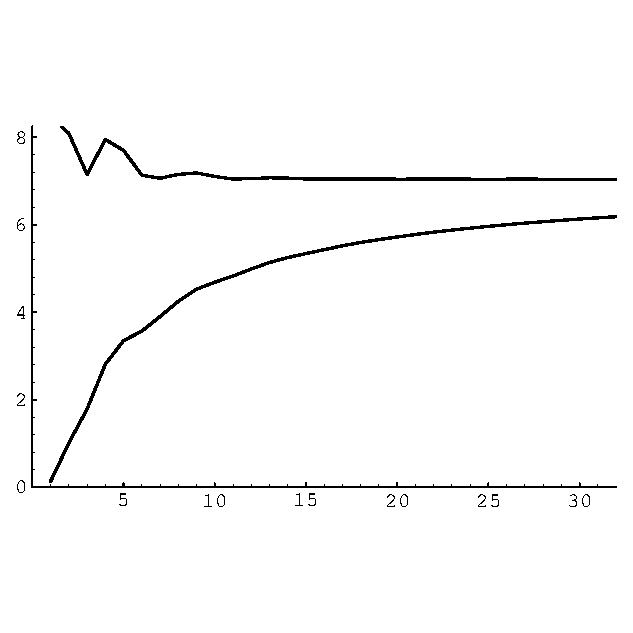
\includegraphics[width=3.25in]{graeffeb}
\end{center}
\caption{Upper and lower bounds on $M(P)$\label{Graeffe:Bound:Fig}}
\end{figure}

The lower bound of \propref{Graeffe:Bound:Prop} is not particularly
sharp, although the upper bound can be made quite sharp by increasing the
size of $k$.  

To illustrate this technique consider the following polynomial
suggested by \cite{Cerlienco1987-vl}
\[
P(X)  = X^6 + X^5 + 6X^4 - 5X^3 + 3X^2 + 2,
\]
which has zeroes
\[
-0.9015 \pm 2.4962 i, \quad0.6745 \pm 0.5646i, \quad
-0.2730 \pm 0.5408i.
\]
Only the first two zeroes are outside the unit circle and their
product is $7.0436280 = M(P)$.  \figref{Graeffe:Bound:Fig} shows the
upper and lower bounds on $M(P)$ based on $P_k$ as $k$ ranges from $1$
to $32$.  For $k = 11$ we already get the quite good upper bound of
$7.0470$, while the lower bound is $4.8284$.  For $k = 2048$, the
lower bound rises to $7.02934$, but computationally this is quite
expensive, due to the size of the coefficients of $P_m(X)$.

\section{Weighted Coefficient Bounds}
\label{Weighted:Bounds:Sec}


The relationship between $|p_i|$ and $M(P)$ given in
\eqnref{CoefZ:Bound:Eq} can be used to derive a bound on the
individual coefficients of divisors of a polynomial, as noted by
Mignotte \cite{Mignotte1974-oa}.  

\begin{proposition}[Mignotte]\label{Mignotte:Bound:Prop}
Let $Q(X) = q_0 X^{r} + q_{1} X^{r-1} + \cdots + q_{r}$ be a
polynomial over $\C$ that divides $P(X)$.  Then
\[
\left| q_{i} \right| \le \binom{r}{i} \left\|P\right\|.
\]
\end{proposition}
\begin{proof}
By \eqnref{CoefZ:Bound:Eq} we have,
\[
|q_i| \le \binom{r}{i} M(Q).
\]
Since every zero of $Q$ is a zero of $P$, we have $M(Q) \le M(P)$, and
by \propref{Landau:Zeroes:Prop}, $M(P) \le \|P\|$, which gives the
proposition. 
\end{proof}

This proposition indicates that the coefficients closer to the middle
of $Q(X)$ can be substantially larger than coefficients near the
leading and trailing terms.  Recently, this observation was made
substantially more precise by using the {\em weighted $L_2$ norm}.

Comparing the definition of the $[\cdot]_2$ norm \eqnref{PB:Beauzamy:Eq} 
with the lower inequality in \eqnref{CoefZ:Bound:Eq} we see that
\[
\sum_{0\le i \le d} \binom{d}{i}^{-1} |p_i|^2 \le
\sum_{0\le i \le d} \binom{d}{i} M^2(P).
\]
So, $[P]_2 \le 2^{d/2} M(P)$.  Applying the inequality to $M(P_1 P_2) = 
M(P_1) M(P_2)$, where $\deg P_1 + \deg P_2 = d$ gives:
\[
2^{d/2} \sqrt{d+1} |P_1 P_2| \ge [P_1]_2 \, [P_2]_2.
\]
More sophisticated techniques \cite{Beauzamy1990-yo} can be used to prove the 
following proposition.

\begin{proposition}
Let $f$ and $g$ be polynomials in one variable of degree $m$ and $n$
respectively.  Then
\[
[fg]_2 \ge \sqrt{\frac{m! \, n!}{(m+n)!}} [f]_2 \, [g]_2,
\]
and this result is best possible.
\end{proposition}

The following proposition \cite{Beauzamy1992-ts} is an analogue of 
\propref{Mignotte:Bound:Prop}, but uses the $[\cdot]_2$ norm. 

\begin{proposition} 
Let $P(X)$ be a univariate polynomial in $X$ over $\Z$, with
non-vanishing constant term.  Let $Q(X)$ be a divisor of $P(X)$, also
with rational integer coefficients.  Denote $\deg P$ by $d$, and $m =
\deg Q$.  Then each coefficient $q_i$ of
$Q(X)$ satisfies
\[
|q_i| \le \sqrt{\frac{1}{2} \binom{m}{i} \binom{d}{m}} [P]_2
   \le \sqrt{\frac{n!}{2(d-m)!\, (m-i)!\, i!}} [P]_2.
\]
Furthermore, 
\[
|Q| \le \frac{3^{3/4}}{2\sqrt{\pi}}\, \frac{3^{d/2}}{\sqrt{d}} [P]_2.
\]
\end{proposition}


\section{Size of a Polynomial's Zeroes}
\label{PB:RootSize:Sec}

The following inequality is due to {\Cauchy}
\cite{Cauchy1829-wp}.\Marginpar{Need intro}

\begin{proposition}[Cauchy]
\label{Cauchy:Zero:Bound:Prop}
Let $P(X) = X^{d} + p_{1} X^{d-1} + \cdots + p_{d}$ be a non-constant,
monic polynomial with coefficients in $\C$.  Then each root of $P(X)$,
$\alpha$, satisfies the inequality
\begin{equation}
\label{Cauchy:Zero:Ineq:Eq}
\left|\alpha\right| < 1 + \max \{|p_{1}|, \ldots, |p_{n}|\} 
  = 1 + \left| P \right|.
\end{equation}
\end{proposition}

\begin{proof}
Assume $|\alpha|$ is greater than $1$, otherwise the proposition is obvious.
By taking the absolute value of 
\[
\alpha^d = -(p_{1} \alpha^{d-1} + \cdots + p_{n}),
\]
we have
\[
\left| \alpha \right|^{d} = \left| p_{1} \alpha^{d-1} + \cdots + p_{n} \right|
 \le \left| \alpha^{d-1} + \cdots + 1 \right| |P| 
 \le { |\alpha|^{d} \over |\alpha| - 1} |P|.
\]
Since $|\alpha| > 1$, we can multiply by $|\alpha| - 1$ which gives 
$|\alpha| \le 1 + |P|$. 
\end{proof}

In \propref{Cauchy:Zero:Bound:Prop} we assumed that $P(X)$ is monic.  If this is not the case, we
can monicize the polynomial and apply \propref{Cauchy:Zero:Bound:Prop}.  In
particular, let 
\[
P(X) = p_{0} X^{d} + \cdots + p_{d},
\]
and let $\alpha$ be a zero of $P(X)$.  Applying the proposition to
\[
X^{d} + \frac{p_{1}}{p_{0}}X^{d-1} + \cdots + \frac{p_{d}}{p_{0}}
\]
gives
\[
\begin{aligned}
|\alpha| & 
   \le 1 + \max\{ \frac{p_{1}}{p_{0}}, \ldots, \frac{p_{d}}{p_{0}} \},\\
 & \le \frac{\left|p_{0}\right| + 
               \max \{\left|p_{1}\right|, \ldots, \left|p_{d}\right|
\}}{\left|p_{0}\right|}.
\end{aligned}
\]
Applying \propref{Cauchy:Zero:Bound:Prop} to the monic polynomial of
$1/\alpha$:
\[
X^{d} + \frac{p_{d-1}}{p_{d}} X^{d-1} + \cdots + \frac{p_{0}}{p_{d}}
\]
gives
\[
|\alpha| \ge \ \frac{\left|p_{d}\right|}{\left|p_{d}\right| + 
   \max\{ \left|p_{0}\right|, \ldots, \left|p_{d-1}\right|\}}.
\]
Putting these two results together we have for each zero of $P(X)$,
\[
\frac{\left|p_{0}\right| + 
               \max \{\left|p_{1}\right|, \ldots, \left|p_{d}\right|
\}}{\left|p_{0}\right|}
\ge
|\alpha| \ge \ \frac{\left|p_{d}\right|}{\left|p_{d}\right| + 
   \max\{ \left|p_{0}\right|, \ldots, \left|p_{d-1}\right|\}}.
\]

\section{Discriminants and Zero Separation}
\label{PB:RootSeparate:Sec}

This section obtains bounds on the minimum difference between zeroes of a
polynomial $P(X)$.  One of the most useful expressions involving the
difference of zeroes of $P(X)$ is the {\em discriminant} of $P$, which
is essentially the square of the product of differences of pairs of
zeroes of $P(X)$.  This quantity is quite useful in the study of
algebraic extensions.

\paragraph{Discriminants}

As usual, let $\alpha_1, \ldots, \alpha_d$ denote the zeroes of
$P(X)$.   Consider the \keyi{Vandermonde matrix}
\[
P_D = 
\left(\begin{array}{ccccc}
1 & \alpha_1 & \alpha_1^2 & \cdots & \alpha_1^{d-1} \\
1 & \alpha_2 & \alpha_2^2 & \cdots & \alpha_2^{d-1} \\
\vdots & & \vdots & \cdots & \vdots \\
1 & \alpha_d & \alpha_d^2 & \cdots & \alpha_d^{d-1} 
\end{array}\right),
\]
which is discussed in some detail in
\sectref{Vandermonde:Sec}.  Its determinant is equal to the product of
the difference of the zeroes of $P(X)$:
\[
\det P_D = \prod_{1\le i < j \le d} ( \alpha_i - \alpha_j).
\]
The {\em discriminant} of $P(X)$\index{discriminant!of a
polynomial} is defined to be
\addsymbol{$\protect\Dscr(P)$}{The discriminant of the polynomial $P$}
\begin{equation}\label{PB:Discriminant:Eq}
\Dscr(P) = p_0^{2d-2} \det|P_D|^2.
\end{equation}

The discriminant of a polynomial can be computed using
resultants.  We write $P(X)$ as
\[
P(X) = p_0 (X - \alpha_1) (X - \alpha_2) \cdots (X - \alpha_d).
\]
Its derivative is
\[
P'(X) = p_0(X - \alpha_2) \cdots (X - \alpha_d) + \cdots + p_0(X - \alpha_1) \cdots (X -
\alpha_{d-1}).
\]
Evaluating at $\alpha_i$ we have
\[
P'(\alpha_i) = p_0(\alpha_i - \alpha_1) \cdots \widehat{(\alpha_i -
\alpha_i)} \cdots (\alpha_i - \alpha_d),
\]
where the circumflex indicates a term in the product that is omitted.
Taking the product over all zeroes of $P(X)$ gives
\[
\begin{aligned}
P'(\alpha_1) \cdots P'(\alpha_d) 
  & \displaystyle
    = (-1)^{d(d-1)/2} p_0^d \prod_{1\le i< j \le n}(\alpha_i - \alpha_j)^2,\\
  & \displaystyle
    = (-1)^{d(d-1)/2} p_0^{2-d} \Dscr(P).
\end{aligned}
\]
By the definition of the resultant \eqnref{Resultant:Def:Eq} 
(page \pageref{Resultant:Def:Eq})
\[
\res_X (P(X), P'(X)) = p_0^{d-1}P'(\alpha_1) \cdots
P'(\alpha_d),
\]
since either $d$ or $d-1$ is even.  Combining these two equations gives
\[
\Dscr(P) = (-1)^{d(d-1)/2} \frac{\res_X (P(X), P'(X))}{p_0}.
\]

This formula allows us to compute the discriminant of specific
polynomials quite readily.  In particular,
\[
\begin{aligned}
\Dscr(aX^2 + bX + c) & = b^2 - 4ac, \\
\Dscr(X^3 + bX + c)  & = -(27 c^2 + 4b^3).
\end{aligned}
\]
For binomial polynomials we have,
\[
\begin{aligned}
\Dscr(X^n +a) &= (-1)^{n(n-1)/2} \res_X(X^n + a, n X^{n-1}), \\
 & = (-1)^{n(n-1)/2} \res_X(X^n + a, n) \res_X(X^n + a, X)^{n-1}, \\
 & = (-1)^{n(n-1)/2} n^n a^{n-1},
\end{aligned}
\]
where we have used \longpropref{Resultant:Properties:Prop}.

For trinomials the computation is a bit more difficult, but we do have
the following result of {\Swan} \cite{Swan1962-lf}.

\begin{proposition}[Swan]
Let $m$ and $n$ be positive integers with {\sc gcd} $d$ and cofactors
$M$ and $N$ respectively.  Then
\[
\begin{aligned}
\Dscr(X^m & + aX^n +b)\\
  & =
 (-1)^{m(m-1)/2} b^{n-1} (m^M b^{M - N} - (-1)^M (m - n)^{M - N} n^N a^M)^d.
\end{aligned}
\]
\end{proposition}
\begin{proof}
By the definition of the discriminant we have
\[
\Dscr(X^m + aX^n +b) 
    = (-1)^{m(m-1)/2} \res_X (X^m + aX^n + b, mX^{m-1} + anX^{n-1}).
\]
Since
\[
X^m + a X^n + b = \frac{X}{m} \cdot \left( mX^{m-1} + a n
X^{n-1}\right)
  + a \frac{m - n}{m} X^n + b,
\]
we have
\[
\begin{aligned}
\Dscr(X^m &+ aX^n +b) \\
  & = (-1)^{m(m-1)/2}  m^{m-n} \res_X (a \frac{m - n}{m} X^n + b, mX^{m-1} + anX^{n-1}).
\end{aligned}
\]
The resultant in this expression can be evaluated by factoring
\[
mX^{m-1} + a n X^{n-1} = X^{n-1} \times (m X^{m-n} + a n),
\]
and computing the two resultants:
\[
\res_X (a \frac{m - n}{m} X^n + b, X^{n-1}) = b^{n-1}
\]
and 
\[
\begin{aligned}
\res_X &(a \frac{m - n}{m} X^n + b, mX^{m-n} + an)\\
  &\qquad\qquad\qquad\qquad =
\left(b^{M-N} m^N - (-1)^N \left(a \frac{m-n}{m}\right)^{M-N} a^N
n^N\right)^d
\end{aligned}
\]
using \longpropref{Binomial:Result:Prop}.
When these results are multiplied and expanded we get the proposition.
\end{proof}

\medskip
Using \longpropref{Resultant:Bound:Prop} we can bound $|\Dscr(P)|$ as
\begin{equation}\label{PB:DiscrmBound1:Eq}
|\Dscr(P)| \le (\deg P + \deg P')! \,|P|^{d-1} |P'|^d \le (2d-1)! \,d^d\,
|P|^{2d-1}.
\end{equation}


This bound can be sharpened by applying the \key{Hadamard inequality}
(\longpropref{Hadamard:Ineq:Prop}) to $P_D$.  First, let $\alpha_i$ be a 
zero of $P(X)$ with absolute value less than $1$.  For each row
of $P_D$, we have
\[
\|\langle 1, \alpha_i, \ldots \alpha_i^{d-1} \rangle\|_2
\le \sqrt{1^2 + 1^2 + \cdots + 1^2} \le \sqrt{d}.
\]

Now, assume the zeroes of $P(X)$ satisfy
\[
|\alpha_1| \ge |\alpha_2| \ge \cdots \ge |\alpha_m| \ge 1 \ge |\alpha_{m+1}|
\ge \cdots \ge |\alpha_d|.
\]
So, the first $m$ zeroes of $P(X)$ lie outside the unit disk.
Dividing the first row by $\alpha_1^{d-1}$, the second row by
$\alpha_2^{d-1}$ and so on, we have
\[
Q_D = \frac{P_d}{(\alpha_1 \cdots \alpha_m)^{d-1}} =
\left(\begin{array}{ccccccc}
\alpha_1^{1-d} & \alpha_1^{2-d} & \alpha_1^{3-d} & \cdots & 1 \\
\vdots & & \vdots & \cdots & \vdots \\
\alpha_m^{1-d} & \alpha_m^{2-d} & \alpha_m^{3-d} & \cdots & 1 \\
1 & \alpha_{m+1} & \alpha_{m+1}^2 & \cdots & \alpha_{m+1}^{d-1} \\
\vdots & & \vdots & \cdots & \vdots \\
1 & \alpha_d & \alpha_d^2 & \cdots & \alpha_d^{d-1} 
\end{array}\right),
\]
where each element of $Q_D$ has absolute value less than $1$.  By
Hadamard's inequality, $\det|Q_D|$ can be bounded by $d^{d/2}$.
Thus,
\[
\det|P|= (\alpha_1 \cdots \alpha_m)^{d-1} \det|Q_D| \le 
\frac{M(P)^{d-1}}{p_0^{d-1}} d^{d/2},
\]
in general.  This immediately gives the following upper bound for the
discriminant. 

\begin{proposition}
If $P(X)$ is a univariate polynomial over $\C$ of degree $d$ and
leading coefficient $p_0$ then the absolute value of the discriminant
of $P(X)$ is bounded by
\[
|\Dscr(P)| \le d^d M(P)^{2(d-1)} \le d^d \|P\|^{2(d-1)}.
\]
\end{proposition}

The last inequality follows from \propref{Landau:Zeroes:Prop}.  Lower
bounds for the discriminant are much more subtle.  We quote the
following results of {\Odlyzko} in this regard \cite{Odlyzko1975-do,Odlyzko1977-rt}:

\begin{proposition}
Let $P(X)$ be a univariate, square free polynomial over $\Z$ of degree
$d$.  Denote the number of real zeroes of $P(X)$ by $r_1$ and the
number of complex zeroes by $2r_2$.  Then
\[
\begin{aligned}
|\Dscr(P)| & \ge (60.1)^{r_1} (22.2)^{2r_2} e^{-254}, \\
|\Dscr(P)| & \ge (58.6)^{r_1} (21.8)^{2r_2} e^{-70}. \\
\end{aligned}
\]
Assuming the generalized Riemann hypothesis
\[
|\Dscr(P)| \ge (188.3)^{r_1} (41.6)^{2r_2} e^{-3.7\times10^8}.
\]
\end{proposition}


\paragraph{Zero Separation}

In order to numerically determine the zeroes of $P(X)$, a univariate
polynomial of degree greater than $1$, it is important to know when
two zeroes are identical.  Since we cannot have exact finite numerical
representations of the zeroes of $P(X)$, we need a lower bound on how
close two distinct zeroes of a $P(X)$ can be.  We define the {\em zero
  separation}\index{zero separation} of $P$ to be
\[
\Delta(P) = \min_{i \not= j} \left| \alpha_{i} - \alpha_{j} \right|.
\]
\addsymbol{$\Delta(P)$}{minimum zero separation of two distinct zeroes
of the univariate polynomial $P$}

Assume that $|\alpha_i - \alpha_j|$ is the difference of roots of
$P(X)$, $i < j$.  We will use a slight variation of the techniques
used for discriminants to get an upper bound on $\det|P_D/(\alpha_i -
\alpha_j)|$.  This immediately yields a lower bound on $\Delta(P)$. 

Start with $P_D$ and subtract the $j$-th row from the $i$-th row,
\[
\left(\begin{array}{ccccccc}
1 & \alpha_1 & \alpha_1^2 & \cdots & \alpha_1^{d-1} \\
\vdots & & \vdots & \cdots & \vdots \\
0 & \alpha_i - \alpha_j & \alpha_i^2 - \alpha_j^2 & \cdots &
\alpha_i^{d-1} - \alpha_j^{d-1} \\
\vdots & & \vdots & \cdots & \vdots \\
1 & \alpha_d & \alpha_d^2 & \cdots & \alpha_d^{d-1} 
\end{array}\right).
\]
$\alpha_i - \alpha_j$ divides the $i-th$ row of this matrix so
\[
\frac{\det|P_D|}{\alpha_i - \alpha_j} = 
\left(\begin{array}{ccccccc}
1 & \alpha_1 & \alpha_1^2 & \cdots & \alpha_1^{d-1} \\
\vdots & & \vdots & \cdots & \vdots \\
0 & 1 & q_2 & \cdots & q_{d-1} \\
\vdots & & \vdots & \cdots & \vdots \\
1 & \alpha_d & \alpha_d^2 & \cdots & \alpha_d^{d-1} 
\end{array}\right),
\]
where 
\[
q_{\ell} = \alpha_i^{\ell-1} + \alpha_i^{\ell -2} \alpha_j + \cdots +
\alpha_j^{\ell-1}.
\]
We now divide the first $m$ rows by $\alpha_{\ell}^{d-1}$ as before.
The elements of all but the $i$-th row have absolute value no
greater than $1$.  The absolute values of the elements of the $i$-th
are bounded by $0, 1, 2, \ldots, {d-1}$ respectively, since
$|\alpha_i| > |\alpha_j|$.  

Applying Hadamard's inequality gives
\[
\frac{\det|P_D|}{(\alpha_i - \alpha_j) (\alpha_1 \ldots
\alpha_m)^{d-1}} 
\le d^{(d-1)/2}\sqrt{0^2 + 1^2 + \cdots + (d-1)^2}.
\]
The sum of squares inside the square root is easily bounded:
\[
0^2 + 1^2 + \cdots + (d-1)^2 = \frac{m(m-1)(2m-1)}{6} \le
\frac{m^3}{3}.
\]
Thus,
\[
\frac{p_0^{d-1} \det|P_D| \sqrt{3}}{M(P)^{d-1} d^{(d+2)/2}} 
   < |\alpha_i - \alpha_j|.
\]
Applying \eqnref{PB:Discriminant:Eq} gives {\Mahler}'s bound on the separation 
of the roots of $P(X)$ \cite{Mahler1964-vy}.

\begin{proposition}[{\Mahler}]
Let $p(x)$ be a square free polynomial of degree $d$ with discriminant $D$.
Then
\[
\Delta(p) > \sqrt{\frac{3 |D|}{d^{d+2}}} M(p)^{1-d}
\]
\end{proposition}

Using \propref{Landau:Zeroes:Prop} we have
\[
\Delta(p) > \sqrt{\frac{3 |D|}{d^{d+2}}} \|p\|^{1-d}.
\]

\section*{Notes}

\small

\notesectref{PB:Heights:Sec} Emma {\LehmerE} \cite{Lehmer1936-dj} surveyed
the early work on the size the coefficients in cyclotomic
polynomials. {\BatemanPT} gave an upper bound on the size of the
coefficients of a cyclotomic polynomial.  They are bounded above by
\[
\log A_n <  \frac{1}{2} d(n) \log n  
\le \frac{1}{2} \frac{(\log 2) (\log n)^2}{\log \log n},
\]
where $A_n$ is the absolute value of the largest coefficient in the
$n$-th cyclotomic polynomial.  Here we have used the bound
\eqnref{DivisorUBound:Eq} in the final inequality.  {\Vaughn}
\cite{Vaughan1974-vf} gave explicit lower bound,
\[
\log A_n > \exp \left( \frac{(\log 2) (\log n)}{\log \log n} \right),
\]
which implies both results are best possible.
{\Apostol} \cite{Apostol1975-js} contains a good bibliography of more
recent results.

\notesectref{Uniform:Bounds:Sec}  A nice proof of
\propref{Jensen:Formula:Prop} is contained in problems 120 and 175,
part III of P\'olya and Szeg\"o \cite{Polya1976-hx}.
{\Gelfond}'s proof of \propref{Factor:CBound:Prop}
\cite{Gelfond1960-ev} (pages 135--139) uses only elementary
techniques but it is quite a bit more lengthy than the one provided
here.

Mignotte \cite{Mignotte1992-sr} gives a bound similar to
\propref{Landau:Zeroes:Prop} but which uses a product of the $n$
largest roots, not all the roots. 

Alternative, more efficient approaches to the Graeffe method of
computing $M(P)$ are discussed in \cite{Cerlienco1987-vl}.  One interesting
observation that can be made from \figref{Graeffe:Bound:Fig} is that
the $\|P_k\|^{1/k}$ tends to be an especially good bound on $M(P)$
when $k$ is a prime number.  Can this statement be made more precise
and generalized?\Marginpar{Also checkout \cite{Boyd93a,Boyd93b,Mignotte94}.}

\notesectref{PB:RootSeparate:Sec} The presentation here follows that
of {\Mahler}'s original paper \cite{Mahler1964-vy}.
{\Mahler}'s proposition gives a lower bound on the separation of any pair 
of zeroes of a polynomial.  If a bound is only needed for a separation of 
real roots, then a bound of {\Rump} can be used that is a bit sharper 
\cite{Rump1979-dt}:
\[
\Delta_{real}(P) > \sqrt{\frac{8}{d^{d+2}}} \, \left(\frac{1}{1+|P|^d}\right).
\] 
\normalsize

    %$Id: zero-test.tex,v 1.1 1992/05/10 19:35:22 rz Exp rz $
\chapter{Zero Equivalence Testing}
\label{Zero:Testing:Chap}

This chapter begins the discussion of ``modern'' algorithms that take
advantage of the sparsity of multivariate polynomials.  These
algorithms do not perform arithmetic operations with the polynomials
directly, but rather compute with the values of the polynomials at
selected points.  They produce the value of the final answer at these
points and then reconstruct the answer from the values.  This approach
eliminates \key{intermediate expression swell} and, when done
properly, only requires time polynomial in the size of the answer.
This is often called a \keyi{black box} model of computation since the
polynomials are treated as opaque boxes---how the values of the
polynomial are computed is not available to us.

In order to highlight the most important points this chapter
considers the simplest problem to which these methods
apply---determining when a polynomial is identically zero.  We call
this the \keyi{zero equivalence problem}.
\chapref{Interpolation:Chap} discusses interpolation schemes that
reconstitute univariate polynomials from their values and
\chapref{Sparse:Interp:Chap} discusses how this is done for
multivariate polynomials by taking sparsity into account.  In
\chapref{Poly:GCD:Chap} these methods are applied to the computation
of polynomial {\sc gcd}'s.  The discussion of the other major modern
scheme for dealing with sparsity begins with \chapref{Hensel:Chap}.

The study of large sparse problems is very much like the study of very
large physical objects (galaxies or black holes) or very small
physical objects (nuclear particles).  They are largely intractable,
and cannot be studied directly.  However, information about the
objects can be obtained indirectly, by their effect on other
computations.  Consider a situation where there is a quantity we wish
to study $P(X_1, \ldots, X_v)$, but where direct computation of $P$
is impractical.  By evaluating $P$ at certain points, we can still
study $P$ indirectly.

As an example of how this might arise, assume we are given $M$, a
square matrix over $\F_p[X_1, \ldots, X_v]$, with determinant $P(X_1,
\ldots, X_v)$.  How would we determine if $M$ is singular; \ie, if
$P$ is identically zero?  If $M$ is large (\eg, $100 \times 100$ with 
polynomial entries), explicitly computing $P$ is impractical due to
\key{intermediate expression swell}.  However, given elements of
$\F_p$, $a_1, \ldots, a_m$, it is relatively easy to determine $P(a_1,
\ldots, a_m)$, since it is an element of $\F_p$.  (We can compute the 
determinant of a $100\times 100$ matrix over a finite field directly using 
Gaussian elimination.)  Thus it is relatively easy to compute the values 
of $P$, but not $P$ itself.  The matrix $M$ can be viewed as a 
representation of a function that computes the value of $P$ at a point.

In this situation, we say that $P$ is represented by a \keyi{black
box} that returns the value of $P$ when given values for its
arguments.  When using a black box representation of a polynomial,
evaluation using the black box is the only way to inspect the
polynomial.  To be more precise, let $P(X_1, \ldots, X_v)$ be some
symbolic expression over a ring $R$.  ${\cal B}_P$ is a \keyi{black
box} representing $P$ if, for $x_1, \ldots, x_v \in \R$,  ${\cal
B}_P(x_1, \ldots, x_v)$ returns $P(x_1, \ldots, x_v)$.  Most often
$P(X_1, \ldots, X_v)$ is a polynomial, but rational and algebraic
functions are also possible.\Marginpar{This paragraph needs work.}

Let $\vec{a}$ be a $v$-tuple.  If ${\cal B}_P(\vec{a})$ is non-zero
then $P$ is not the zero polynomial.  However, the converse is not
true.  However unlikely, $\vec{a}$ may still accidently be chosen to
be a zero of $P$.  By quantifying the likeliness of accidently
choosing a zero of $P$, we can develop a {\em probabilistic}
algorithm for zero equivalence.  These techniques are discussed in
\sectref{Zero:Probabilistic:Sec}.

When we have a bound on the maximum number of non-zero terms in $P$,
the zero equivalence problem is called the {\em zero equivalence
problem with term bounds\/}.\index{zero equivalence problem! with term
bounds} This problem can be solved by deterministic algorithms that
take time polynomial in the size of $P$.  These techniques, which are
discussed in \sectref{Zero:Deterministic:Sec}, can be used to prove
that certain problems can be solved in polynomial time.  For most
practical problems, however, the probabilistic algorithms are more
useful.

Throughout this chapter and the next we assume polynomials are
represented in expanded form, as a list of monomials (pairs of
exponent-vectors and coefficients), and that monomials with zero
coefficients are omitted.  We denote the number of variables in a
polynomial by $v$, so the exponent vectors are $v$-tuples.  The
maximum degree of $X_i$ in $P$ is denoted by $d_i$ and the maximum of
the $d_i$ is denoted by $d$.  Occasionally, it is necessary to work
with polynomials for which we have \keyi{total degree bounds} instead
of individual degree bounds for each variable.  This bound is usually
given by $D$.  We always have
\[
d \le D \le vd.
\]

The number of non-zero monomials of the polynomial $P$ is usually
denoted by $t$ or $\terms P$.  The number of terms in a possibly
sparse polynomial is bounded by the number of terms in a dense
polynomial:
\[
\terms P \le (d+1)^v.
\]
Occasionally we will need to distinguish between the actual number of
terms in a polynomial and an {\em a priori} bound on the number of
terms in a polynomial.  We will use $T$ to denote the {\em a priori}
bound, and $t$ to denote the actual number of non-zero terms present
in $P$.
\addsymbol{$\terms P$}{The number of terms in the polynomial $P$}

There is a problem when analyzing the cost of algorithms that use
black boxes: How should we account for the cost of the black box
computation?  Different black boxes will require different amounts of
computation.  At best, we can parameterize this cost.  The most common
approach is merely to count the number of black box invocations.  For
example we might say that an algorithm requires ``$O(n^3)$ arithmetic
operations and invokes the black box $O(n)$ times.''  The second
approach is to assume that there is an exponent $\BBoxExp$ such
that the cost of a black box invocation on an input of size $w$ is
bounded by $O(w^{\BBoxExp})$.  With this convention, the cost of the
same algorithm might be $O(n^3 + n^{\BBoxExp})$.  If $\BBoxExp \le 3$,
then the resulting algorithm requires $O(n^3)$ operations. 


\section{Probabilistic Techniques}
\label{Zero:Probabilistic:Sec}

Without any bounds on the number of terms or the degree of the
variables in the polynomial $P$ and given only the black box ${\cal
B}_P$, one can provide substantial evidence that $P$ is the zero
polynomial by showing that ${\cal B}_P(\vec{a})$ returns zero for many
randomly chosen $v$-tuples $\vec{a}$.  In order to provide a
probabilistic algorithm for zero equivalence, we need to quantify how
strong this evidence actually is.

The only way that the evidence provided by ${\cal B}_P$ can be
misleading is if ${\cal B}_P$ returns $0$ when $P$ is actually
different from zero.  The following proposition quantifies how often
this can occur. It is the basis of nearly all the probabilistic
algorithms in computer algebra.

\begin{proposition}\label{Prob:Zero:Prop}
Let $A$ be an integral domain, $P$ a non-zero element of
$A[X_1,\ldots, X_v]$ and the degree of $P$ in each of $X_i$ be bounded
by $d_i$.  Let $Z_n(B)$ be the number of zeroes of $P$, $\vec{x}$ such
that $x_i$ is chosen from a set with $B$ elements, $B \gg d$.  Then
\[
\begin{aligned}
  Z_n(B) &\le B^v - (B-d_1)(B-d_2) \cdots (B-d_v)\\
    & \le (d_1 + d_2 + \cdots + d_v) B^{v-1}.
\end{aligned}
\]
\end{proposition}

\begin{proof}
There are at most $d_v$ values of $X_v$ at which $P$ is identically
zero.  So for any of these $d_v$ values of $X_v$ and any value for the
other $X_i$, $P$ is zero.  This comes to $d_vB^{v-1}$.  For all other
$B-d_v$ values of $X_v$ we have a polynomial in $v-1$ variables.  The
polynomial can have no more than $Z_{v-1}(B)$ zeroes.  Therefore,
\[
Z_v(B) \le d_v B^{v-1} + (B - d_v) Z_{v-1}(B).
\]

Rather than solving this recurrence for $Z_v$, we solve it for $N_v =
B^v - Z_v$.  Since $Z_1$ is less than or equal to $d_1$, $N_v \ge (B -
d_1)$.  This is the basis step of the inductive proof.  Writing the
recurrence in terms of $N_v$ we have
\[
B^v - N_v(B) \le d_v B^{v-1} + (B - d_v) (B^{v-1} - N_{v-1}(B))
\]
or
\[
N_v(B) \ge (B - d_v) N_{v-1}(B),
\]
from which the proposition follows. 
\end{proof}

The following polynomial actually has $B^v - (B-d_1) \cdots (B-d_v)$
zeroes with components less than $B$
\[
P(X_1, \ldots, X_v) =
\prod_{0 \le i_1 \le d_1}(X_1 - x_{1i}) \quad \cdots 
\prod_{0 \le i_v \le d_1}(X_v - x_{1v}).
\]
Thus the first inequality in the proposition cannot be further
strengthened.  

For the analysis of some algorithms the results of this theorem are
more useful when expressed in terms of probabilities.  We denote the
probability that $P$ is zero for $(x_1, \ldots, x_v)$, chosen randomly,
by
\[
{\cal P}(P(x_1, \ldots, x_v) = 0 \mid x_i \in {\cal S})
= \frac{Z_v(B)}{B^n} \le \frac{d_1 + \cdots d_v}{B}.
\]

Sometimes a similar bound is needed, but in terms of the total degree of
the polynomial $P$.\index{total degree, of a polynomial}  This bound
is provided by the following proposition.

\begin{proposition} \label{Prob:Total:Zero:Prop}
Let $P \in A[X_1, \ldots, X_v]$ be a polynomial of
total degree $D$ over an integral domain $A$.  Let ${\cal S}$ be a
subset of $A$ of cardinality $B$.  Then
\[
{\cal P}(P(x_1, \ldots, x_v)=0 \mid x_i \in {\cal S}) \le \frac{D}{B}.
\]
\end{proposition}

\begin{proof}
We use induction on the number of variables as was done in the proof
of the previous proposition.  For $v= 1$, $f$ is a univariate
polynomial of degree $D$ and can have no more than $D$ zeroes in $A$,
so 
\[
{\cal P}(P(x_1)=0 \mid x_1 \in {\cal S}) \le \frac{D}{B}.
\]

Assume the proposition is true for polynomials in $v-1$ variables.
Let the degree of $P$ in $X_v$ be $d_v$ and denote the leading
coefficient of $f$ with respect to $X_v$ by $f_0$, \ie,
\[
P = p_0(X_1, \ldots, X_{v-1}) X_v^d + \cdots.
\]
The total degree of $p_0$ is no more than $D - d$, so the probability
that $p_0 = 0$ is
\[
{\cal P}(p_0(x_1, \ldots, x_{v-1})=0 \mid x_i \in {\cal S}) \le \frac{D-d}{B}.
\]

Omitting the arguments of $x_1, \ldots, x_v$ and $x_1, \ldots,
x_{v-1}$ for brevity, we can write
\[
\begin{aligned}
{\cal P}(P =0) &= 
  {\cal P}(P =0 \wedge p_0=0) \cdot {\cal P}(p_0=0) \\
  & \qquad \qquad+
  {\cal P}(P=0 \wedge p_0\not=0) \cdot {\cal P}(p_0\not=0), \\
   & \le {\cal P}(p_0=0) + {\cal P}(P=0 \wedge p_0\not=0).
\end{aligned}
\]
Assume that $p_0(x_1, \ldots, x_{v-1})\not=0$. $P(x_1, \ldots,
x_{v-1}, X_v)$ is a polynomial of degree $d$, so there are at most $d$
$x_v \in {\cal S}$ such that $P(x_1, \ldots, x_v) = 0$. Consequently,
\[
{\cal P}(P(x_1, \ldots, x_{v})=0 \mid x_i \in {\cal S}) \le \frac{D -
d}{B} + \frac{d}{B} = \frac{D}{B}.
\]
\end{proof}


The following proposition phrases the result of
\propref{Prob:Zero:Prop} as a probability.

\begin{proposition} \label{Zero:MPoly:Prop}
Let $f_1, f_2, \ldots, f_s$ be elements of $A[X_1, \ldots, X_v]$, $A$
an integral domain, where the degree in each variable is bounded by
$d$.  Let ${\cal P}(f_1, \ldots, f_s)$ be the probability that a
randomly chosen point $\vec{x}$ is a zero of any of the $f_i$, where
$x_i$ is an element of a set with $B$ elements.  Then
\[
{\cal P}(f_1, \ldots, f_s) < \frac{vds}{B}.
\]
\end{proposition}

\begin{proof}
Let $f = f_1 f_2 \cdots f_s$.  The degree of each variable in $f$ is
bounded by $ds$.  Applying the previous proposition, we see that the
number of zeroes of $f$ is bounded by $vdsB^{v-1}$, for sufficiently
large $B$.  Since there are $B^v$ possible $\vec{x}$ from which to
choose, we have the corollary.
\end{proof}

\medskip
\propref{Zero:MPoly:Prop} gives a probabilistic algorithm for zero
equivalence.  We only indicate that a polynomial is non-zero when
${\cal B}_P$ returns a non-zero value, proving that $P$ is non-zero.
We want to know the probability that ${\cal B}_P$ returns zero even
though $P$ is not identically zero.  Assume that $P$ is not the zero
polynomial.

Define the set ${\cal S}_B$ to be
\[
{\cal S}_B = \{\,(x_1, \ldots, x_v) \mid 0 \le x_i < B\,\}.
\] 
Let $\vec{x}$ be an element of ${\cal S}_B$ such that ${\cal B}_P$
returns zero.  Then $\vec{x}$ is one of the at most $Z_v(B)$ zeroes in
of $P$ in ${\cal S}_B$.  If we choose $\vec{x}$ randomly, the
probability that we will get a zero of $P(\vec{X})$ is 
\[
{vD \over B},
\]
where the $D \ge \max(d_i)$.  The probability that $k$ randomly chosen
elements of ${\cal S}_B$ would all yield a value of zero (even though
$P$ is not the zero polynomial) is less than $(vD/B)^k$.

To verify that a polynomial $P(X_1, \ldots, X_v)$, whose degree in
each variable is less than $D$, is zero with probability less than
$\epsilon$ we need to perform $k$ evaluations with random elements of
${\cal S}_B$ where
\begin{equation}
\epsilon < \left({v D \over B}\right)^k. 
\label{Bound:Eq}
\end{equation}
A single evaluation will suffice if $B$ is chosen such that $B \ge
vD/\epsilon$.  The cost of the single evaluation is the cost of the
black box evaluation.  Recall that the cost of a black box evaluation
with $v$-tuple components of size $w$ is $O(w^{\BBoxExp})$, for some
$\BBoxExp$.  Since the size of the components of the random $v$-tuple is
$\log vD/\epsilon$, the cost of a single evaluation is
$O(\log^{\BBoxExp} v D/\epsilon)$.  If $k$ different evaluations are
used, then we need to choose $B$ such that \eqnref{Bound:Eq} is
satisfied.  So,
\[
\log B < \log vD + {1 \over k} \log {1 \over \epsilon}.
\]
The cost of a single evaluation when $k$ are intended is
\[
O\left(\log^{\BBoxExp} {vD \left({1 \over \epsilon}\right)^{1/k}}\right),
\]
and the total time required for $k$ evaluations using the
probabilistic approach will be 
\[
C_{\rm prob} 
   = O\left(k \log^{\BBoxExp} {vD \left({1 \over \epsilon}\right)^{1/k}}\right).
\]
This quantity is minimized when
\begin{equation}\label{Zero:PCount:Eq}
k = {({\BBoxExp} - 1) \log{1 \over \epsilon} \over \log vD}.
\end{equation}
Since $1/\epsilon \gg vD$, using multiple evaluations with relatively
small evaluation points is better than a single evaluation at a
large evaluation point. 

Replacing $k$ by this quantity in $C_{\rm prob}$ we have
\[
\begin{aligned}
C_{\rm prob} &= 
O\left({({\BBoxExp}-1) \log {1\over \epsilon} \over \log vD}
 \log^{\BBoxExp} {vD \left({1 \over
\epsilon}\right)^{ \log vD \over ({\BBoxExp}-1) \log {1\over \epsilon}}}\right)
\\
& = O\left({\log {1 \over \epsilon} \over \log vD} 
  \log^{\BBoxExp}  (vD)^{1+{1\over {\BBoxExp}-1}}\right)\\
& = O(\log {1 \over \epsilon} \times \log^{{\BBoxExp}-1} vD).
\end{aligned}
\]
Notice that the cost of the probabilistic algorithm is linear in the
logarithm of the error.  This is a good characterization of what it
means for a probabilistic algorithm to be polynomial time.

\medskip
Using the ideas in this section, the following routine
probabilistically checks to see if ${\cal B}_P$ represents a polynomial
that is identically zero.  The probability that this routine returns
an incorrect answer is controlled by the parameter $\epsilon$.  The
number of variables and the degree of the variables in $P$ is
indicated by $v$ and $D$ respectively.
\begindsacode
PZeroEquiv(${\cal B}_P$, $v$, $D$, $\epsilon$) := $\{$\\
\> $k \leftarrow  4 (\log 1/\epsilon)/(\log vD)$; \\
\> loo\=p for $0 \le i < k$ do \{ \\
\>\> if ${\cal B}_P(2^i, 3^i, \ldots, p_v^i) \not=0$ then return(false); \\
\>\> $\}$\\
\> return(true);\\
\> $\}$
\enddsacode

\noindent
Notice that in \keyw{PZeroEquiv} we have replaced $\BBoxExp - 1$ in
\eqnref{Zero:PCount:Eq} by $4$.  From a practical point of view this is
quite reasonable.  It is unlikely that the code in ${\cal B}_P$ would
have an exponent larger than $5$.

\section{Deterministic Results}
\label{Zero:Deterministic:Sec}

The probabilistic zero equivalence algorithm discussed in the previous
section is, from a practical point of view, quite sufficient.  However,
from a theoretical perspective it is desirable to know when the zero 
equivalence problem can be decided in \keyi{deterministic polynomial 
time}.  Given ${\cal B}_P$, a black box for the polynomial 
$P(X_1, \ldots, X_v)$ and degree bounds on $P$, only probabilistic 
algorithms are possible.  In essence this is because there are too many 
possible coefficients in $P$ and thus too many degrees of freedom to 
eliminate in polynomial time.  This is made more precise in 
\sectref{Zero:Negative:Sec}.  However, given a bound on the number of 
non-zero terms in $P$, there exist deterministic algorithms for zero 
equivalence. 

The first deterministic zero equivalence algorithm was
developed by {\Grigoriev} and {\Karpinski} \cite{Grigoriev87}.  It is
quite simple and does not even require degree bounds for the
polynomial---only a term bound.  However, this algorithm only works for 
polynomials over $\Z$ (though it is easily generalized to unique 
factorization domains).  The second algorithm, due to {\Zippel} 
\cite{Zippel90}, works over more general domains, but requires a degree 
bound in addition to the term bound. 

Assume we are given a black box for a polynomial, ${\cal B}_P$ and
want to determine if $P$ is identically zero.  The
only interaction the algorithm has with the black box is to pass it an
evaluation point and look at the result.  If the black box ever
returns a non-zero value, then $P$ is not identically zero and the
algorithm can terminate.  The sequence of test values used by the
algorithm cannot depend in any adaptive fashion on the responses from
${\cal B}_P$, since the responses will always be zero and thus do not depend
upon ${\cal B}_P$.  The sequence of test values {\em is} the
algorithm.  A sequence of test values that identifies the character of
a class of black boxes is called a \keyi{characterizing sequence}.  In
\sectref{Zero:Probabilistic:Sec} we proved that random sequences are
{\em likely} to characterize a black box, but this is not assured.

The two algorithms discussed here use different characterizing
sequences, but in both cases the sequences are based on the following 
proposition.

\begin{proposition}\label{Zero:Mon:Prop}
Let $P(\vec{X})$ be a non-zero polynomial in $R[\vec{X}]$ with at most
$T$ terms and with monomial exponent vectors $\vec{e}_i$.  Assume there
exists an $n$-tuple $\vec{x}$ (in some $R$-module) such that the
$\vec{x}^{\vec{e_i}}$ are distinct.  Then not all of $P(\vec{x}^0),
P(\vec{x}), P(\vec{x}^2), \ldots, P(\vec{x}^{T-1})$ are zero.
\end{proposition}

\begin{proof}
Denote $\vec{x}^{\vec{e}_i}$ by $m_i$.  By assumption, each of the
$m_i$ are distinct.  If $P$ vanished at each of the $\vec{x}^i$ then
the following system of linear equations would hold.
\[
\begin{aligned}
  c_1 + c_2 + \cdots + c_T &= 0 \\
  c_1 m_1 + c_2 m_2 + \cdots + c_T m_T &= 0\\
  c_1 m_1^2 + c_2 m_2^2 + \cdots + c_T m_T^2 &= 0\\ \vdots\\
  c_1 m_1^{T-1} + c_2 m_2^{T-1} + \cdots + c_{T} m_T^{T-1}&=0
\end{aligned}
\]
Since this is a Vandermonde system and we have assumed that the $m_i$
are distinct, the system of equations is non-singular.  Thus the $c_i$
must all be zero, and $P$ must be identically zero for all of
$P(\vec{x}^0), P(\vec{x}), P(\vec{x}^2), \ldots, P(\vec{x}^{T-1})$ to 
vanish.
\end{proof}


\paragraph{Without Degree Bounds}

The remaining problem is finding a substitution that keeps the
monomials distinct.  The technique of {\Grigoriev} and {\Karpinski} is
quite simple.  It is based on the observation that the rational
integers are a unique factorization domain. Thus if $p$ and $q$ are
\key{prime numbers} then $p^{e_1} q^{f_1}$ is equal to $p^{e_2} q^{f_2}$ if 
and only if $e_1= e_2$ and $f_1 = f_2$.  Since this keeps the terms 
distinct, by \propref{Zero:Mon:Prop}, it is a distinguishing set of 
evaluation points.  The following proposition makes this precise.

\begin{proposition}[{\Grigoriev} and {\Karpinski}]
\label{Deterministic:Zero:Prop}
Let $P(\vec{X})$ be a polynomial in $v$ variables over a ring of
characteristic zero, $A$, and assume that $P$ has no more than $T$
monomials.  Then there exists a set of $v$-tuples, $\{\vec{x}_0,
\ldots,
\vec{x}_{T-1}\}$ such that either $P(\vec{x}_i) \not= 0$ for some 
$\vec{x}_i$ or $P$ is identically zero.
\end{proposition}

\begin{proof}
Let $\vec{x} = (2, 3, 5, \ldots, p_v)$, where the entries are the 
canonical images of the prime numbers of $\Z$ in $A$.  By unique 
factorization of $\Z$, the monomials $\vec{x}^{\vec{e}_i}$ are distinct, 
and thus by \propref{Zero:Mon:Prop} either $P$ is identically zero or 
does not vanish at every element of the set $\{\vec{x}^0, \ldots,
\vec{x}^{T-1}\}$.
\end{proof} 

\propref{Deterministic:Zero:Prop} gives a simple deterministic
solution of the zero equivalence problem with term bounds.  We merely
pass each of the trial points $\vec{x}_0, \ldots, \vec{x}_{T-1}$ to ${\cal
B}_P$. If ${\cal B}_P$ returns an answer different from zero then $P$
is not the zero polynomial.  If ${\cal B}_P$ returns zero for all of
the trial points then it is the zero polynomial.
\begindsacode
GKZ\=eroEquiv(${\cal B}_P$, $n$, $T$) := $\{$\\
\> loo\=p for $0 \le i < T$ do \{ \\
\>\> if ${\cal B}_P(2^i, 3^i, \ldots, p_v^i) \not=0$ then return(false); \\
\>\> $\}$\\
\> return(true);\\
\> $\}$
\enddsacode

\keyw{GKZeroEquiv} requires $T$ evaluations using ${\cal B}_P$, the
last of which involves numbers as large $p_v^{T-1}$.  Since we have no
idea what computation is going on inside of ${\cal B}_P$ there is no
way to estimate the cost of each of the $T$ evaluations.  Thus the
most precise statement we can make about cost of {\tt GKZeroEquiv} is
that it requires $T$ evaluations and no other arithmetic operations.

Nonetheless, we can get some understanding of the \keyi{bit complexity} 
of using such 
large evaluation points by assuming that ${\cal B}_P$ simply
computes each of the monomials in $P$ and then adds up the values.  On
average, the $n$-th prime is no larger than $n \log n$ by the prime
number theorem.  So, the $k$-th evaluation by ${\cal B}_P$ will
require $O\left(M(k \log (n \log n))\right)$ time, where $M(K)$ is the
time to multiply two $K$ bit numbers.  For simplicity, we assume $M(K)
= K^2$.  Thus all $T$ evaluations require
\[
\sum_{k=0}^{T-1} O(k^2 \log^2 (v \log v))  = O(T^{3} \log^2 (v \log v))
\]
time.  Thus the complexity of \keyw{GKZeroEquiv} is dominated by the 
number of non-zero terms, not the degree of the polynomials.

The following proposition generalizes \propref{Deterministic:Zero:Prop} to 
the zero avoidance  problem for several polynomials.\Marginpar{Use development from lecture notes 4/18/95 for the following proposition.}

\begin{proposition}
\label{Interp:15:Prop}
Let $P_1(\vec{X}), \ldots, P_s(\vec{X}) \in A[X_1, \ldots, X_v]$ be
non-zero polynomials over a ring of characteristic zero, $A$, and
assume that 
\[
\terms P_1 + \cdots + \terms P_s = T.
\]
Let $\vec{x}$ be the image of $(2, \ldots, p_n)$ in $A^n$.  Then for some 
integer $j$, $0 \le j \le T$, all of $P_i(\vec{x}^j)$ are different from zero.
\end{proposition}

\begin{proof}
Denote the points $\{ \vec{x}^0, \vec{x}, \ldots, \vec{x}^T\}$ by
${\cal S}$.  $P_i$ cannot vanish at more than $\terms P_i$ elements of
${\cal S}$ by \propref{Deterministic:Zero:Prop}.\Marginpar{Do I need the generalized vanderonde results here? (prop. 114)}  Since ${\cal S}$
contains $T+1$ points, there must be one for which none of the $P_i$
vanish. 
\end{proof}

\paragraph{With Degree Bounds}

An alternate approach to the zero equivalence problem was developed 
independently by {\Grigoriev}, {\Karpinski} and {\Singer} 
\cite{Grigoriev90} and {\Zippel} \cite{Zippel90}.  The approaches in 
these two papers are almost 
identical, but with one slight variation that will be mentioned later.
The basic idea is that rather than showing that $P(\vec{X})$ is
non-zero, we choose a substitution $X_i \mapsto Z^{e_i}$ and show that
$P(Z^{\vec{e}})$ is non-zero.  This polynomial is univariate and has no
more non-zero terms than the original multivariate polynomial.
Proving that it is non-zero is relatively easy.

The crucial part of this technique is showing that the substitution
$\vec{X} \mapsto Z^{\vec{u}}$ does not send the non-zero polynomial
$P(\vec{X})$ to the zero polynomial, and furthermore that the degree
of $P(Z^{\vec{u}})$ is not too large.  To do this several different
substitutions are required.  All that we can prove is that if
$P(\vec{X})$ is not identically zero then one of the resulting
univariate polynomials will not be zero.

To illustrate the basic ideas, consider a simple version of this
technique that follows the approach used in the previous section.
Assume $R$ is a field, so $R[Z]$ is a unique factorization domain and
$Z+1, Z+2, \ldots$ are primes. Denote by $\vec{Z}$ the vector $(Z+1,
Z+2, \ldots, Z+v)$.  Thus the $\vec{Z}^{\vec{e}_i}$ are distinct.
Sending
\begin{equation}\label{Zero:LinearSubs:Eq}
(X_1, \ldots, X_v) \mapsto (Z+1, \ldots, Z+v) = \vec{Z}
\end{equation}
maps $P(\vec{X})$ into a univariate polynomial.  Since the $Z+i$ are
primes in a unique factorization domain, $\vec{Z}^0, \vec{Z}^1,
\ldots, \vec{Z}^{T-1}$ is characterizing sequence for any polynomial
$P$, with $T$ non-zero terms by \propref{Zero:Mon:Prop}.  In this
section we call the substitution of \eqnref{Zero:LinearSubs:Eq} a
\keyi{linear substitution}.

Unfortunately, this characterizing sequence yields a sequence of
univariate polynomials $P(\vec{Z}^i)$, each of whose degree is bounded
by $ivD$.  Since a univariate polynomial of degree $N$ cannot vanish
at more than $N$ values, each $P(\vec{Z}^i)$ can be characterized by
$ivD+1$ different values of $z$.  Combining these two steps gives the
following deterministic algorithm

\begindsacode
SD\=ZeroEquiv(${\cal B}_P$, $v$, $D$, $T$) := $\{$\\
\>loo\=p for $0 \le i < T$ do \{ \\
\>\> loo\=p for $0 \le z \le ivD$ do \{ \\
\>\>\> if \=${\cal B}_P((z+1)^i, (z+2)^i, \ldots, (z+v)^i) \not= 0$ \\
\>\>\>\>then return(false); \\
\>\>\> \}\\
\>\> \}\\
\> return(true); \\
\> \}
\enddsacode

\keyw{SDZeroEquiv} is a deterministic algorithm for zero equivalence,
but it requires that $R$ contain $vDT+1$ distinct elements if the
inner loop is modified appropriately.  When this is possible, it
generates a characterizing sequence of length $O(vDT^2)$.

When the coefficient field is contained in $\R$, we can improve the
number of evaluations required to characterize a univariate
polynomial.  The key is {\Descartes}' rule of signs:

\begin{proposition}[Descartes]
\label{Descartes:Sign:Prop}
Let $C$ denote the number of sign changes in the polynomial $p(x) \in
\R[x]$ and $Z$ the number of positive real zeroes.  Then $C - Z$ is a
non-negative even integer.
\end{proposition} 


Let $P(Z)$ be a univariate polynomial with $T$ non-zero
terms and denote the number of sign changes among its coefficients by
$C$.  Then $C$ is bounded above by $T-1$.  Applying
\propref{Descartes:Sign:Prop} gives 
\[
0 \le C - N_Z \le T - 1 - N_Z,
\]
which is stated as the following proposition.

\begin{proposition}
\label{Positive:Zeroes:Prop}
Let $P(x)$ be a univariate polynomial with coefficients in $\R$.  The
number of positive real zeroes of $P(x)$ is less than $\terms(P)$.
\end{proposition}

By choosing the evaluation points to be positive numbers the length of
the characterizing sequence for $P$ can be reduced from $\deg P$ to
$\terms P$, which can be much smaller.  The technique of {\tt
SDZeroEquiv} unfortunately, generates dense univariate polynomials.
By using a more sophisticated substitution we can reduce a
multivariate polynomial to a univariate polynomial that has no more
non-zero terms than the original multivariate polynomial.  This
technique will yield a characterizing sequence of length $O(vT^2)$ for
polynomials over $\R$.

\medskip
Instead of using the simple linear substitution of
\eqnref{Zero:LinearSubs:Eq}, we use:
\begin{equation} \label{Zero:MultiSub:Eq}
(X_1, X_2, \ldots, X_v) \longrightarrow
  (Z^{u_1}, Z^{u_2}, \ldots, Z^{u_v})
\end{equation}
where the $u_i$ are positive integers.  We call
\eqnref{Zero:MultiSub:Eq} a \keyi{nonlinear substitution}.  The
nonlinear substitution sends monomials in $P(\vec{X})$ to univariate
monomials in $Z$, so that $P(Z^{\vec{u}})$ has no more non-zero terms
than $P(\vec{X})$.  The difficulty is finding a vector $\vec{u}$ such
that $P(Z^{\vec{u}})$ is not identically zero.

The key idea is that the exponents $u_1, \ldots, u_v$ should come from a
large set of maximally independent $v$-tuples.

\begin{definition}
Let $\cal U$ be a set of $v$-tuples with components in $\Z$.
$\cal U$ is said to be \keyb{maximally independent} if every subset of
$v$ elements of $\cal U$ is $R$-linearly independent.
\end{definition}

In our situation, each element of $\cal U$, $\vec{u}$, corresponds to
a substitution $X_i \mapsto Z^{u_i}$.  If ${\cal U}$ is sufficiently
large, then some element $\vec{u} \in {\cal U}$ will lead to a
polynomial $P(Z^{\vec{u}})$ that is not identically zero.  The
following proposition shows that there exist arbitrarily large sets of
maximally independent $v$-tuples and that the components of the
$v$-tuples are not large.

\begin{proposition}
\label{SPMod:Lemma:1:Prop}
Let $S$ be a positive integer and $p$ be the smallest prime number
larger than $S$.  There exists a maximally independent set of $S$
$v$-tuples where each of the components of the $v$-tuples is less than
$p$.
\end{proposition}

\begin{proof}
First we show that we can construct arbitrarily large maximally
independent sets of $v$-tuples.  Then by reducing them modulo a prime
we get $v$-tuples of the size required by the proposition. Consider
$v$-tuples of the form $(1, k, k^2, \ldots, k^{v-1})$.  For $v$ of
these to be independent the determinant of the matrix
\[
\begin{pmatrix}
1& k_1 & k_1^2 & \cdots & k_1^{v-1}\\
1& k_2 & k_2^2 & \cdots & k_2^{v-1}\\
\vdots& &\vdots& & \vdots\\
1& k_v & k_v^2 & \cdots & k_v^{v-1}\end{pmatrix}
\]
must not be zero.  Since this is a \key{Vandermonde matrix}, it is
nonsingular if and only if the $k_i$ are different.  This and further
results on Vandermonde matrices are given in
\sectref{Vandermonde:Sec}.

Thus, if the $k_i$ are distinct then the vectors they generate will be
linearly independent.  In particular if we let $\vec{u}_k = (1, k,
\ldots, k^{v-1})$ then any subset of $n$ of the $\vec{u}_k$ will be
linearly independent.  Furthermore, if we reduce the elements of $\vec
u_k$ by $p$ the $k_i$ remain distinct modulo $p$ then the $v$-tuples
remain maximally independent.\Marginpar{This needs to be clarified a bit.}
\end{proof}

The size of the elements of the maximally independent set depend upon
the size of $p$.  By \key{Bertrand's postulate}
(\longpropref{Bertrands:Post:Prop}) there exists a $p$ greater than
$S$ and less than $2S$.  

In \cite{Grigoriev90} essentially identical techniques are used, but
the Vandermonde matrix used in the previous proposition is replaced by
the \keyi{Cauchy matrix} whose determinant is
\begin{equation}\label{Zero:Cauchy:Eq}
\det\left|
  \begin{array}{cccc}
\frac{1}{a_1+b_1} & \frac{1}{a_1+b_2} & \cdots & \frac{1}{a_1+b_v} \\[3pt]
\frac{1}{a_2+b_1} & \frac{1}{a_2+b_2} & \cdots & \frac{1}{a_2+b_v} \\[3pt]
\vdots & \vdots & & \vdots \\[3pt]
\frac{1}{a_v+b_1} & \frac{1}{a_v+b_2} & \cdots & \frac{1}{a_v+b_v} 
\end{array}\right|
=
\prod_{1\le i < j \le v}\frac{(a_j - a_i) (b_j - b_i)}{(a_i + b_j)}.
\end{equation}
As long as the $a_i$ and $b_j$ are (separately) distinct every square
submatrix of the Cauchy matrix will be non-singular and thus its rows will
be linearly independent.  Letting $a_i = 1, \ldots, S$ and $b_j = 1,
\ldots, v$ we get a sequence  of $S$ maximally independent vectors:
\[
(\frac{1}{2}, \frac{1}{3}, \ldots, \frac{1}{v+1}), 
(\frac{1}{3}, \frac{1}{4}, \ldots, \frac{1}{v+2}), \ldots
(\frac{1}{S+1}, \frac{1}{S+2}, \ldots, \frac{1}{S+v}).
\]
Again choosing a prime $p > S$ and reducing the components of each
vector by $p$ gives a sequence of vectors that satisfy
\propref{SPMod:Lemma:1:Prop}.  

For simplicity, we define ${\cal U}_{S,v}$ to be a set of maximally
independent $v$-tuples, where the components of each vector are
positive and less than $2S$.  Let $p$ be a prime such that $S < p
<2S$.  The previous discussion shows that either of the following
constructions of ${\cal U}_{S,v}$ can be used:
\[
{\cal U}_{S,v} =
\begin{array}{l}
  \{\, (1, i, i^2\mod p, \ldots, i^{v-1} \mod p) \mid 1 \le i \le v \,
\} \\[4pt]
  \{\, ((i+1)^{-1} \mod p, \ldots, (i+v)^{-1} \mod p) 
      \mid 1 \le i \le v \,\}
\end{array}
\]

\medskip
The following proposition uses the elements of the set ${\cal
U}_{nT,v}$ to construct univariate characterizing sequences for sparse 
polynomials.

\begin{proposition}\label{Sparse:ZeroPoly:Prop}
For every non-zero polynomial $P(X_1, \ldots, X_v)$ with no more than
$T$ non-zero terms and the degree of each $X_i$ bounded by $D$ there is a $\vec{u}$ in ${\cal U}_{vT,v}$ such that
$P(Z^{\vec{u}})$ is not identically zero.  Furthermore, the degree of
$P(Z^{\vec{u}})$ is less than $2v^2DT$ and $P(Z^{\vec{u}})$ has no
more than $T$ non-zero terms.
\end{proposition}

\begin{proof}
Let the non-zero terms of $P$ be
\[
P(\vec{X}) = c_1 \vec{X}^{\vec{e}_1} + c_2 \vec{X}^{\vec{e}_2} 
+ \cdots + c_T \vec{X}^{\vec{e}_T}.
\]
The substitution $X_i \mapsto Z^{u_i}$ transforms this polynomial into
\[
P(Z) = c_1 Z^{\vec{e}_1 \cdot \vec{u}} + c_2 Z^{\vec{e}_2 \cdot \vec{u}} +
\cdots +
c_T Z^{\vec{e}_T \cdot \vec{u}}.
\]
To find a substitution for which $P(Z^{\vec{u}})$ is not identically
zero we require $\vec{u}$ to satisfy
\[
\vec{e}_1 \cdot \vec{u} \not= \vec{e}_i \cdot \vec{u},
\]
or equivalently $(\vec{e}_i - \vec{e}_1) \cdot \vec{u} \not= 0$, for $2
\le i \le T$.  Let $d = \vec{e}_1 \cdot \vec{u}$.  With such a
substitution only the $c_1 \vec{X}^{\vec{e}_1}$ monomial of
$P(\vec{X})$ will be mapped to a term in $P(Z)$ of degree $d$.  Since
$c_1 \not= 0$, $P(Z)$ cannot be identically zero; it must contain a
$Z^d$ term.

Letting $L_i(\vec{w}) = (\vec{e}_i - \vec{e}_1)\cdot
\vec{w}$, $2 \le i < T$ we want to find a $\vec{w}$ at which none of
the $L_i$ vanish. 

Let $\vec{w}_1, \ldots, \vec{w}_v$ be distinct elements of ${\cal
U}_{vT, v}$, so
\[
\begin{pmatrix}\vec{w}_1 \\ \vdots \\ \vec{w}_v \end{pmatrix} \cdot
 (\vec{e}_i - \vec{e}_1)^T
 = 
\mathbf{A}\cdot (\vec{e}_i - \vec{e}_1)^T = 
  \begin{pmatrix}L_i(\vec{w}_1) \\ \vdots \\ L_i(\vec{w}_v) \end{pmatrix}.
\]
Since $\mathbf{A}$ is non-singular, the right hand side can only be zero
if $L_i$ is identically zero.  Thus, $L_i$ cannot vanish for more than
$n-1$ of the elements of ${\cal U}_{vT,v}$.  There are $T-1$ $L_i$'s.
Since $(v-1)\cdot (T-1)$ is less than $vT$, there must be at least one
element of ${\cal U}_{vT, v}$ for which none of the $L_i$ vanish as
desired.  We denote such an element by $\vec{u}$.  Each of the
components of $\vec{u}$ is less than $2nT$, while the elements of
$\vec{e}_i$ are less than $D$.  Thus the degree of $P(Z^{\vec{u}})$ is
less than $2v^2DT$.
\end{proof}

Using the univariate polynomial constructed in
\propref{Sparse:ZeroPoly:Prop} and the univariate polynomial zero test 
given by \propref{Positive:Zeroes:Prop}, we can construct the
following zero equivalence algorithm for black box polynomials over
the reals.

\begindsacode
RDZeroEquiv(${\cal B}_P$, $v$, $T$) := $\{$\\
\>loo\=p for $\vec{u} \in {\cal U}_{vT,v}$ do \{ \\
\>\> loo\=p for $1 \le z \le T$ do \{ \\
\>\>\> if \=${\cal B}_P(z^{u_1}, z^{u_2}, \ldots, z^{u_v}) \not= 0$ \\
\>\>\>\>then return(false); \\
\>\>\> \}\\
\>\> \}\\
\> return(true); \\
\> \}
\enddsacode

\begin{figure}
\begin{center}
\begin{tabular}{l|c|c|c|c|}
\multicolumn{1}{c}{} 
& \multicolumn{1}{c}{\# poly} & \multicolumn{1}{c}{\# terms} &
 \multicolumn{1}{c}{degree} & \multicolumn{1}{c}{\# points} \\ \cline{2-5}
Linear & $T$ & $\le vDT$ & $\le vDT$ & $vDT^2+T$ \\ \cline{2-5}
Nonlinear & $vT$ & $\le T$ & $\le v^2DT$ & $vT^2$ \\ \cline{2-5}
\end{tabular}
\end{center}
\caption{Complexity of different multivariate to univariate substitutions\label{Mult:Uni:Fig}}
\end{figure}

The table in \figref{Mult:Uni:Fig} illustrates the difference between
these two methods for black boxes over rings of characteristic zero.
Using the linear substitution \eqnref{Zero:LinearSubs:Eq} requires
generating $T$ polynomials of degree as large as $vDT$.  Since the
polynomials are dense the characterizing sequence of each must be of
length $vDT+1$ and the entire characterizing sequence for the black
box is of length $vDT^2+T$.  The non-linear substitution
\eqnref{Zero:MultiSub:Eq} produces more polynomials ($vT$) and
polynomials of greater degree, but each has no more than $T$ non-zero
terms.  By using positive integers as evaluation points, we get a
characterizing sequence of length $vT^2$.

\paragraph{Finite Fields}

If the characteristic of the coefficient domain is positive, then the
zero testing problem becomes a bit harder.  Consider, for instance,
the polynomial $M(X) = X^p - X$.  Even though $M(X)$ only has two
terms it vanishes for every element of $\F_p$.  Nonetheless,
\propref{Zero:Mon:Prop} is true for polynomial over fields of positive
characteristic.  The difficulty in this case is that there are no
values of $X$ that distinguish the two monomials of $M(X)$, $X^p$ and
$X$.  This problem does not arise for polynomials over fields of
characteristic zero, since there are many elements that distinguish
$X^m$ and $X^n$ when $m \not= n$.

This issue means that it is not possible to do {\em deterministic}
zero testing for polynomials over a finite field {\em without degree
bounds\/}.  However, the problem is solvable if we have degree bounds
on the black box.  

As usual, let ${\cal B}_Q$ be a black box for a polynomial $Q$.
Assume $Q$ is a univariate polynomial of degree $d$, with $T$ terms,
with coefficients in $\F_p$:
\[
Q(X) = q_1 X^{e_1} + q_2 X^{e_2} + \cdots + q_T X^{e_T},
\]
where $e_i \le d$.  Using \propref{Zero:Mon:Prop}, the sequence of
evaluation points, $1, m, m^2, \ldots$ will be a distinguishing
sequence if each of the values 
\[
m^{e_1}, m^{e_2}, \ldots, m^{e_T}
\]
are distinct. If the multiplicative order of $m$ is greater than $d$,
then these values are certainly distinct.

Now the problem is finding element of multiplicative order greater
than $d$.  In the case of $M(X) = X^p - X$, there is no such element
in $\F_p$ and thus there is no way to distinguish $M(X)$ from $0$
using a test sequence chosen from $\F_p$.  The solution to this
problem is to enlarge the ground field $\F_p$ to $\F_{p^k}$ which does
have elements of order $d$.  For instance, $\F_{p^2}$ has $\phi(p^2 -1)$
elements of order $p^2 -1$ any of which can be used to distinguish $M(X)$
from $0$.

In general there are three cases.  First, if the characteristic of the
ground field is very large, $p > 2^d$, then $m = 2$ will suffice.

Second, if $p$ is small we allow algorithms that are polynomial in
$p$.  The ground field $\F_p$, can be expanded by adjoining an element
of degree $k$ over $\F_p$, where $p^k > d$.  By
\propref{FF:AlgExtOrder:Prop} the field $\F_{p^k}$ has 
\[
\varphi(p^k -1) \approx \frac{6}{\pi^2} p^k -1
\]
elements of order $p^k -1$.  So with approximately $\lceil
\pi^2/6\rceil = 2$ random choices we should be able to find an
element of $\F_{p^k}$ whose multiplicative order is $p^k -1$.

Third, if $p$ is very large we cannot afford to find a multiplicative
generator of $\F_{p^k}$.  In this case we take the opposite approach,
and construct a very large degree extension of $\F_p$, one of degree
$K$ where $K > d$.  The generator of this extension will serve a good
generator for the irreducibility test.  
{\Adleman} and {\LenstraH} \cite{Adleman86} have shown that there
exists a positive integer $c$ such 
that using $(k \log p)^c$ steps one can find 
an irreducible polynomial of degree $d$ such that
\[
\frac{k}{c \log p} < d \le k.
\]
So, sufficiently large extensions can be found in polynomial
time.  %%\Marginpar{Needs work}

\section{Negative Results}
\label{Zero:Negative:Sec}

The zero equivalence problem with only degree bounds, and no bound on
the number of terms, is not solvable in deterministic polynomial time.
This is because it is too easy to find polynomials that vanish at a
large number of prescribed points and which still have small degree.
This is shown in the following proposition.

\begin{proposition}
\label{Key:Negative:Prop}
Let $D$, $T$ and $v$ be integers such that $D^v > T$.  Let ${\cal S} =
\{\vec{a}_i \}$ be a set of $T-1$ $v$-tuples.  There exists a
polynomial with rational integer coefficients with no more than $T$
non-zero monomials and that vanishes at each point in $\cal S$.
\end{proposition}

\begin{proof}
In fact, there are many polynomials that satisfy the requirements.
Choose a set of $T$ distinct $v$-tuples, $\vec{e}_1, \ldots, \vec{e}_T$,
where each component is an element of $\{0, 1, \ldots, D\}$.  The
polynomials with these exponents are all of the form 
\[
P(\vec{X}) = c_1 {\vec{X}}^{\vec{e}_1} + c_2 {\vec{X}}^{\vec{e}_2} 
+ \cdots + c_T {\vec{X}}^{\vec{e}_T}.
\]
We claim that at least one of these polynomials vanishes at each point
in ${\cal S}$.  For $P$ to vanish at $\vec{a}_i \in {\cal S}$ the $c_j$
must satisfy the following linear equation:
\[
c_1 {\vec{a}_i}^{\vec{e}_1} + c_2 {\vec{a}_i}^{\vec{e}_2} + \cdots +
c_T {\vec{a}_i}^{\vec{e}_T} = 0.
\]
Thus $P(\vec{X})$ vanishes at each element of $\cal S$ if the $c_j$
satisfy the following system of linear equations.
\[
\begin{aligned}
c_1 {\vec{a}_1}^{\vec{e}_1} + c_2 {\vec{a}_1}^{\vec{e}_2} + \cdots +
c_T {\vec{a}_1}^{\vec{e}_T} & = 0\\
c_1 {\vec{a}_2}^{\vec{e}_1} + c_2 {\vec{a}_2}^{\vec{e}_2} + \cdots +
c_T {\vec{a}_2}^{\vec{e}_T} & = 0\\
\vdots&\\
c_1 {\vec{a}_{T-1}}^{\vec{e}_1} + c_2 {\vec{a}_{T-1}}^{\vec{e}_2} 
+ \cdots +
c_T {\vec{a}_{T-1}}^{\vec{e}_T} & = 0
\end{aligned}
\]
Since these equations are homogeneous and there are more variables than
equations, the system possesses a non-trivial solution.
\end{proof}

\propref{Key:Negative:Prop} directly implies the non-existence of a
deterministic algorithm for zero recognition.

\begin{proposition}
\label{Black:Box:Prop}
Given a black box representing a polynomial $P(\vec{X})$ in $v$ variables
and of degree less than $D$ in each variable, any deterministic algorithm
that determines if $P$ is the zero polynomial runs in time at least
$O(D^v)$.
\end{proposition}

\begin{proof}
The time required by the algorithm is at least as large the number of
trial evaluations used.  Since no polynomial of degree less than $D$
has more than $D^v$ terms, $D^v$ trials suffice.  Thus the problem can
be solved in exponential time.  By \propref{Key:Negative:Prop}, if the
algorithm uses less than $D^v$ trials there will be polynomials that
meet the degree bounds and that are indistinguishable from the zero
polynomial.  Thus at least $D^v$ trial evaluations are required.
\end{proof}

Though the zero equivalence problem, given degree bounds, is not solvable
in deterministic polynomial time, notice that a polynomial that vanishes at
each of $O(D^v)$ trial points, constructed as in the proof of
\propref{Black:Box:Prop} would have $O(D^v)$ non-zero terms.  It would be
very interesting to know if there exists a polynomial that vanishes at
those trial points and that has a more succinct representation
(straight-line program, for instance).

\begin{figure}
{
\renewcommand{\arraystretch}{1.4}
\begin{center}
\begin{tabular}{l|c|c|}
\multicolumn{1}{c}{} & \multicolumn{1}{c}{Probabilistic}
   & \multicolumn{1}{c}{Deterministic}\\ 
\cline{2-3}
degree bounds & $\log {1 \over \epsilon} \times \log^{r-1} vD$ 
   & $D^v \log^r D$ \\ \cline{2-3}
term bounds & & $T^{r+1} \log^r v$ \\ \cline{2-3}
\end{tabular}
\end{center}
}
\caption{Complexity of Zero Testing\label{Zero:Comp:Fig}}
\end{figure}

The results of this section are summarized in the table in
\figref{Zero:Comp:Fig}.  The columns correspond to probabilistic and
deterministic algorithms respectively.  The rows correspond to whether
degree bounds or term bounds are given.  In the deterministic, bounded
degree case, we have given a lower bound on the time required, while
for the other two entries we have demonstrated algorithms that achieve
the indicated performance.  Also recall that $r$ is a constant
corresponding to the type of arithmetic being used by ${\cal B}_P$.
For classical arithmetic $r=2$; for fast arithmetic $r$ is slightly
greater than $1$.

As remarked earlier, the zero equivalence problem with degree bounds
cannot be solved in deterministic polynomial time, yet it can be
solved in probabilistic polynomial time.  We find it very curious that
with a slight change to the way information is provided, the problem
can be solved in deterministic polynomial time.  The zero equivalence
problem seems to lie on the boundary between those problems that can and
cannot be solved in deterministic polynomial time.  Though earlier
work has shown that random and deterministic polynomial time can be
separated via an oracle \cite{Heller86}, we find this example
interesting because it arises in a common practical problem.

By representing the polynomial as a black box, we have swept the issues of
the size of the computation required to compute $P(\vec{x})$ under the rug.
If we could look inside ${\cal B}_P$ and examine the ``program'' used to
compute $P(\vec{x})$ we might be able to show that ${\cal B}_P$ represents
the zero polynomial without any bounds on $P$.  For example, it seems
likely that one can prove that a straight-line program for a polynomial (in
the sense of {\Kaltofen} \cite{Kaltofen85d}) can be deterministically shown
to represent the zero polynomial in time polynomial in the size of the
straight-line program.



\section*{Notes}

\small

\notesectref{Zero:Probabilistic:Sec} The earliest mention of
probabilistic zero testing that we have been able to find appears in a
1978 note of {\DeMillo} and {\Lipton} on testing algebraic programs
\cite{Demillo78}.  They essentially reproduce \propref{Prob:Zero:Prop}.

Unaware of the prior work of {\DeMillo} and {\Lipton}, {\SchwartzJ}
\cite{Schwartz80} and {\Zippel} \cite{Zippel79a} simultaneously and
independently also proved \propref{Prob:Zero:Prop}.  (Apparently the time 
was ripe for this proposition.)  Their solutions to this problem were 
given in two successively presented papers at the EUROSAM '79 
conference in Marseille during the summer of 1979.  The slightly weaker 
result of the last line of the proposition was proven and used in the 
work of {\SchwartzJ} \cite{Schwartz80}, while that of the first line was 
given by  {\Zippel} \cite{Zippel79a}.

\notesectref{Zero:Deterministic:Sec}
The probabilistic techniques discussed in
\sectref{Zero:Probabilistic:Sec} were a dramatic improvement to the
state of the art in symbolic computation when they were introduced in
1979.  From the theoretical perspective, the work in
\cite{Zippel79b} essentially reduced a number of problems
(polynomial greatest common divisor and polynomial factorization) to
random polynomial time.  Moreover, the reduction led to algorithms
that were more efficient than the existing algorithms.  

For several years, it was believed that these problems were
intrinsically harder than deterministic polynomial time. In
particular, it was believed the zero equivalence problem could not be
solved in deterministic polynomial time.  The results of
\sectref{Zero:Negative:Sec}, which were well understood during the
1980's reinforced this belief.

In 1987 {\Grigoriev} and {\Karpinski}, as part of their work on
bipartite graph matching \cite{Grigoriev87}, developed a deterministic
algorithm for the zero equivalence problem for polynomials with
integer coefficients given a bound on the number of {\em non-zero
terms}.  These ideas where then used by {\BenOr} and {\Tiwari} in 1988
\cite{BenOr88} to produce a deterministic algorithm for interpolation
of sparse polynomials, which is discussed in
\sectref{Interp:BenOr:Sec}.  In 1988, {\Zippel} independently
developed a deterministic algorithm for the zero equivalence problem
with term bounds \cite{Zippel90} (as well as an interpolation
algorithm), which did not have the restrictions of {\Grigoriev} and
{\Karpinski} algorithm.

{\Risler} and {\Ronga} \cite{Risler90} independently developed an
approach similar to that of \cite{Zippel90,Grigoriev90}.

Building on \cite{Heintz80a}, {\Heintz} and {\Schnorr}
\cite{Heintz82a} have shown that there exist short characterizing
sequences for polynomials expressed as straight line programs.
Unfortunately, their techniques do not provide a way to generate these
characterizing sequences.  Determining these sequences is currently
the most important outstanding problem in zero testing.

\normalsize

    %$Id: interp.tex,v 1.1 1992/05/10 19:42:22 rz Exp rz $
\chapter{Univariate Interpolation}
\label{Interpolation:Chap}

The previous chapter showed how to determine if a polynomial was zero
by examining its values at well chosen points.  This chapter develops
techniques to determine the polynomial itself from a sequence of 
values.  This process is called {\em interpolating a polynomial
from its values\/}.  This technique is one of the most useful tools
for constructing efficient symbolic computing algorithms for sparse problems.

In the previous chapter we used knowledge about when Vandermonde matrices
were non-singular to develop deterministic algorithms for zero
testing.  In this chapter we will also need to solve systems of
linear equations whose coefficients form a Vandermonde matrix.
\sectref{Vandermonde:Sec} develops some properties of Vandermonde
matrices and the basic techniques for dealing with Vandermonde style
systems of equations.

We consider two interpolation schemes for univariate polynomials in
the chapter, the \keyi{Lagrange interpolation formula} and the
\keyi{Newton interpolation formula}.  The Lagrange technique follows
directly from Vandermonde techniques discussed in
\sectref{Vandermonde:Sec} and are discussed in
\sectref{Interp:Lagrange:Sec}.  The Newton interpolation scheme arises 
from applying the Chinese remainder algorithm\index{Chinese remainder
theorem} to the values of a polynomial.  It is discussed in
\sectref{Interp:CRA:Sec}.

By choosing the evaluation points in an interpolation scheme
especially carefully, it is possible to interpolate exceedingly
quickly.  This technique, the \key{fast Fourier transform}, is
discussed in \sectref{Poly:FFT:Sec} and is applied to multiplying
polynomials.  This produces the fastest known polynomial multiplication
algorithm.  The complexities of these different algorithms is
summarized in \figref{Interp:Complex:Fig}.

\begin{figure}
\begin{center}
\begin{tabular}{|c|c|c|}
\multicolumn{1}{c}{Algorithm} & \multicolumn{1}{c}{Time} 
  & \multicolumn{1}{c}{Space} \\ \hline
Lagrange & $O(n^2)$ & $O(n)$ \\ \hline
Newton & $O(n^2)$ & $O(n)$ \\ \hline
Fast Fourier  & $O(n \log n)$ & $O(n)$ \\ \hline
\end{tabular}
\end{center}
\caption{Complexity of different interpolation
algorithms\label{Interp:Complex:Fig}}
\end{figure}


In \sectref{Interp:Abstract:Sec} we discuss interpolation from a
somewhat more abstract perspective.  This approach allows us to
combine the Chinese remainder theorem results for integers with those
for polynomials into a single uniform framework.

\section{Vandermonde Matrices}
\label{Vandermonde:Sec}

\index{Vandermonde matrix|(}

Vandermonde matrices have two properties that make them particularly
useful for the algorithms in this chapter: (1) it is easy to ensure
that they are non-singular and (2) systems of linear equations whose
coefficients form Vandermonde matrices are easy to solve exactly. Note
that Vandermonde matrices of floating point numbers can be numerically
quite unstable and these techniques may not be appropriate.

A \keyi{Vandermonde matrix} is a matrix of the form  
\begin{equation} \label{Vandermonde:Eq}
V_n = \begin{pmatrix}
1& k_1 & k_1^2 & \cdots & k_1^{n-1}\\
1& k_2 & k_2^2 & \cdots & k_2^{n-1}\\
\vdots& &\vdots& & \vdots\\
1& k_n & k_n^2 & \cdots & k_n^{n-1}\end{pmatrix},
\end{equation}
where the $k_i$ are chosen from some field.
Similarly, a system of linear equations of the form
\[
\begin{aligned}
X_1 + k_1 X_2 + k_1^2 X_3 + \cdots + k_1^{n-1} X_n &= w_1 \\
X_1 + k_2 X_2 + k_2^2 X_3 + \cdots + k_2^{n-1} X_n &= w_2 \\
\vdots&\\
X_1 + k_n X_2 + k_n^2 X_3 + \cdots + k_n^{n-1} X_n &= w_n 
\end{aligned}
\]
will be called a \keyi{Vandermonde system of equations}.

A matrix where the degrees of each column are the same and within each
row the degrees rise monotonically, is called a {\em generalized
Vandermonde matrix\/},\index{Vandermonde matrix!generalized} \viz,
\[
\begin{pmatrix}
k_1^{e_1}& k_1^{e_2} & k_1^{e_3} & \cdots & k_1^{e_n}\\
k_2^{e_1}& k_2^{e_2} & k_2^{e_3} & \cdots & k_2^{e_n}\\
\vdots& &\vdots& & \vdots\\
k_n^{e_1}& k_n^{e_2} & k_n^{e_3} & \cdots & k_n^{e_n}\end{pmatrix},
\]
where $e_1 < e_2 < \cdots e_n$.  We will often use generalized
Vandermonde matrices where $e_1 = 0$.

The determinant of a \key{Vandermonde matrix} is particularly simple
to compute.  Multiplying the $i$-th column of
\eqnref{Vandermonde:Eq} by $k_1$ and subtracting it from the
$i+1${\st} column gives,
\[
\det V_n = 
  \left|
  \begin{array}{ccccc}
    1&0&0 &\cdots &0\\
    1&k_2 - k_1&k_2^2 -k_1 k_2& \cdots &k_2^{n-1} - k_2^{n-2} k_1 \\
    \vdots&\vdots&\vdots&  & \vdots\\
    1&k_n - k_1&k_n^2 -k_1 k_n& \cdots &k_n^{n-1} - k_n^{n-2} k_1 
  \end{array}\right|.
\]
Expanding by \keyi{Cramer's rule} across the first row and factoring out
$k_i-k_1$ from the $i$-th row we have the following recursive
formula
\[
\begin{aligned}
\det V_n &= \det V_{n-1} \prod_{1<j \le n} \left(k_j - k_1\right), \\
  & = \det V_{n-2} \prod_{2<j \le n} \left(k_j - k_2\right) 
      \prod_{1<j \le n} \left(k_j - k_1\right).
\end{aligned}   
\]
Thus we have:

\begin{proposition}
The determinant of the \key{Vandermonde matrix} is
\[
\det V_n = \prod_{1 \le i < j \le n} \left(k_j - k_i\right).
\]
\end{proposition}

\noindent
As an immediate consequence, the determinant of a \key{Vandermonde matrix}
is non-zero if and only if the $k_i$ are distinct.

\medskip
This result is not true for generalized Vandermonde matrices.  For
instance, for order $2$ matrices we have 
\[
\det V_{2} = 
\left|
\begin{array}{cc}
 1&k_1^e \\ 1 &k_2^e
\end{array}\right| = k_2^e - k_1^e,
\]
which implies that $V_{2}$ is nonsingular if and only if $k_{1}/k_{2}$
is not an $e$-th root of unity.  This is a stronger requirement
than was required for Vandermonde determinants.  In fact, an $n
\times n$ generalized Vandermonde determinant is divisible by the
related Vandermonde determinant.  

Nonetheless, a similar result on the singularity of generalized
Vandermonde matrices over the {\em reals\/}
is true, but the proof is a little trickier.  The following
proposition is only valid over $\R$, which has characteristic zero.
We know of no similar result for fields of positive characteristic.
        
\begin{proposition}
\label{Gen:Vandermonde:Prop}
The determinant of a generalized Vandermonde matrix is non-zero if the
$k_i$ are distinct positive real numbers.
\end{proposition}

\begin{proof}
We show the matrix is non-singular by induction.  A Vandermonde matrix
of order 1 is obviously non-singular since we only allow positive entries.
In the general case we consider a matrix of the form
\[
\begin{pmatrix}
1& k_1^{e_2} & k_1^{e_3} & \cdots & k_1^{e_n}\\
1& k_2^{e_2} & k_2^{e_3} & \cdots & k_2^{e_n}\\
\vdots& &\vdots & & \vdots\\
1& k_n^{e_2} & k_n^{e_3} & \cdots & k_n^{e_n}
\end{pmatrix}.
\]
Replace $k_1$ by the indeterminate $Z$ and consider the number of zeroes of
the polynomial
\[
G(Z) = 
\left|\begin{array}{ccccc}
  1& Z^{e_2} & Z^{e_3} & \cdots & Z^{e_n}\\
  1& k_2^{e_2} & k_2^{e_3} & \cdots & k_2^{e_n}\\
  \vdots& &\vdots & &\vdots\\
  1& k_n^{e_2} & k_n^{e_3} & \cdots & k_n^{e_n}
\end{array}\right| =
a_1 - a_2 Z^{e_2} + a_3 Z^{e_3} - \cdots - a_n Z^{e_n}.
\]
Each coefficient ($a_i$) is a minor of the original matrix and is itself a\Marginpar{This paragraph needs to be fixed up.}
generalized Vandermonde matrix of order $n-1$.  If $k_2, k_3, \ldots , k_n$
are distinct positive numbers then the minors are non-zero by induction.
The polynomial in $Z$ can only have $n-1$ positive zeroes by
\longpropref{Positive:Zeroes:Prop}.  But certainly each of $k_2, k_3, \ldots,
k_n$ is a zero of the polynomial.  Thus there are no other positive
real zeroes and $G(k_1) \not= 0$.
\end{proof}

The inverse of a \key{Vandermonde matrix} can be computed by the
following technique.  Multiply a Vandermonde matrix by a general $n$
by $n$ matrix:
\begin{equation}\label{Vander:InvProd:Eq}
\begin{pmatrix}
1&k_1&k_1^2&\cdots&k_1^{n-1}\\
1&k_2&k_2^2&\cdots&k_2^{n-1}\\
\vdots& & \vdots& & \vdots\\
1&k_n&k_n^2&\cdots&k_n^{n-1}
\end{pmatrix} \cdot
\begin{pmatrix}
p_{11}&p_{12}&p_{13}&\cdots&p_{1n}\\
p_{21}&p_{22}&p_{23}&\cdots&p_{2n}\\
\vdots& & \vdots& &\vdots\\
p_{n1}&p_{n2}&p_{n3}&\cdots&p_{nn}
\end{pmatrix},
\end{equation}
where the $p_{ij}$ are chosen such that this product is equal to the
identity matrix.
The $j$-th element of the top row of the product of these two matrices is
\[
p_{1j} + p_{2j} k_1 + p_{3j} k_1^2 + \cdots + p_{nj} k_1^{n-1} = P_j(k_1),
\]
where $P_j(Z)$ is a polynomial of degree $n-1$ in $Z$.
So, the product \eqnref{Vander:InvProd:Eq} is equal to 
\[
\begin{pmatrix}P_1(k_1)& P_2(k_1) & \cdots & P_n(k_1)\\
P_1(k_2)& P_2(k_2) & \cdots & P_n(k_2)\\
\vdots & \vdots & & \vdots\\
P_1(k_n)& P_2(k_n) & \cdots & P_n(k_n)\end{pmatrix}.
\]
By choosing $P_i(Z)$ such that $P_i(k_j) = 0$ if $i\not= j$ and
$P_i(k_i) =1$ otherwise, the above matrix becomes the identity matrix.
We let $P_j(Z)$ be
\begin{equation} \label{Vander:Pj:Eq}
P_j(Z) = \prod_{\genfrac{}{}{0pt}{2}{i \not= k}{1 \le i \le n}}
  {Z - k_i \over k_j - k_i}.
\end{equation}
The numerator ensures that the off diagonal entries are zero, while
the denominator term ensures that the diagonal terms are one.

\medskip
We demonstrate these ideas by giving an algorithm for solving the following
Vandermonde system of equations: 
\begin{equation}\label{VandermondeSys:Eq}
\begin{aligned}
x_1 + k_1 x_2 + k_1^2 x_3 + \cdots + k_1^{n-1} x_n & = w_1,\\
x_1 + k_2 x_2 + k_2^2 x_3 + \cdots + k_2^{n-1} x_n & = w_2,\\
\vdots\\
x_1 + k_n x_2 + k_n^2 x_3 + \cdots + k_n^{n-1} x_n & = w_n.
\end{aligned}
\end{equation}
When recognized as a Vandermonde system, these equations need only
consume $O(n)$ space since only $k_1, \ldots, k_n$ and $w_1, \ldots,
w_n$ must be stored.  They can be solved using $O(n)$ space as
follows:

Let $\vec{x}$ be the column vector of unknowns $(x_1, \ldots, x_n)^T$
and $\vec{w} = (w_1, \ldots, w_n)^T$.  Then \eqnref{VandermondeSys:Eq}
can be written as
\[
V_n \cdot \vec{x} = \vec{w}.
\]
This equation is solved by multiplying on the left by the inverse of $V_n$:
\[
\left(
\begin{array}{c} x_1 \\ x_2 \\ \vdots \\ x_n \end{array}
\right) =
\left(
 \begin{array}{ccccc}
    p_{11}&p_{12}&p_{13}&\cdots&p_{1n}\\
    p_{21}&p_{22}&p_{23}&\cdots&p_{2n}\\
    \vdots& & \vdots& &\vdots\\
    p_{n1}&p_{n2}&p_{n3}&\cdots&p_{nn}
 \end{array}\right)
\cdot
\left(
\begin{array}{c} w_1 \\ w_2 \\ \vdots \\ w_n \end{array}
\right).
\]
So,
\begin{equation} \label{VanderSol:Eq}
\begin{aligned}
x_i & = p_{i1} w_1 + p_{i2} w_2 + \cdots + p_{in} w_n, \\
     &= \coef(P_1(Z), Z^{i-1}) w_1 + \cdots
       + \coef(P_n(Z), Z^{i-1}) w_n.
\end{aligned}
\end{equation}

This computation can be made quite efficient.  Define the {\em master 
polynomial} 
\begin{equation}
P(Z) = \prod_{1\le i \le n} \left(Z - k_i\right).
\label{Big:Poly:Eq}
\end{equation}
This polynomial contains $n+1$ terms.  The coefficient of $Z^n$ is
always $1$.  Expanding the product in \eqnref{Big:Poly:Eq}
requires $\Theta(n^2)$ arithmetic operations.  

Once $P(Z)$ is known each of the $P_j(Z)$ can be computed
in $O(n^2)$ arithmetic operations.  The numerator of $P_j(Z)$, which
is $P(Z)/(Z - k_j)$, can be computed by classical polynomial division
in $O(n)$ time.  The denominator of $P_j(Z)$, which is the value of
$P(Z)/(Z-k_j)$ at $Z = k_j$, can be computed in $O(n)$ time by
Horner's rule (\sectref{Poly:Subs:Sec}).  Thus each of the $P_j(Z)$
can be computed using $O(n)$ space and time.

The computation of the $x_i$ is arranged as follows.
\[
\begin{pmatrix}x_1\\ \vdots\\ x_n\end{pmatrix} =
\begin{pmatrix}w_1 \cdot \coef(P_1, Z^0) \\  \vdots \\ w_1 \cdot \coef(P_1, Z^{n-1}) \end{pmatrix}
+ \cdots +
\begin{pmatrix}w_n \cdot \coef(P_n, Z^0) \\  \vdots \\ 
         w_n \cdot \coef(P_n, Z^{n-1}) \end{pmatrix}.
\]
After each column vector on the right hand side is computed, it is 
added to the accumulating $X_i$ and its storage may be reused by 
the following column vector.  This approach leads to the following
program:
\begindsacode
SolveVandermonde (k[n], w[n]) := $\{$ \\
\> $Q(Z) \leftarrow   (Z - \mbox{k[$1$]})\times \cdots \times (Z - \mbox{k[$n$]})$; \\
\> $\mbox{x[$\cdot$]} \leftarrow 0$; \\
\> loo\=p for \=$1 \le i \le n$ do \{ \\
\>\> $Q_i(Z) \leftarrow \mbox{PolyQuotient}(Q(Z), Z - \mbox{k[$i$]})$; \\
\>\> $P_i(Z) \leftarrow Q_i(Z)/Q_i(k[$i$])$; \\
\>\> loo\=p for $1 \le j \le n$ do \{ \\
\>\>\> $\mbox{x[$j$]} \leftarrow \mbox{x[$j$]} + \mbox{w[$i$]} \cdot
\coef(P_i(Z), Z^{j-1})$;\\
\>\>\> $\}$ \\
\>\> $\}$ \\
\> return(x); \\
\> $\}$
\enddsacode

As pointed out above, the computation of each $P_i(Z)$ takes $O(n)$
arithmetic operations, so the time complexity of
\keyw{SolveVandermonde} is $O(n^2)$ and only $O(n)$ space is
required.

\medskip
This approach can also be applied to transposed Vandermonde
systems:\index{Vandermonde system!transposed}
\begin{equation}\label{Trans:Vander:Eq}
\begin{aligned}
x_1 + x_2 + x_3 + \cdots + x_n & = w_1,\\
k_1 x_1 + k_2 x_2 + k_3 x_3 + \cdots + k_n x_n & = w_2,\\
\vdots\\
k_1^{n-1} x_1 + k_2^{n-1} x_2 + k_3^{n-1} x_3 +
 \cdots + k_n^{n-1} x_n & = w_n.
\end{aligned}
\end{equation}

Since the inverse of the transpose of a matrix is the transpose of the
inverse, we have the following solution for $\vec{x}$
\[
\left(
\begin{array}{c} x_1 \\ x_2 \\ \vdots \\ x_n \end{array}
\right) =
\left(
 \begin{array}{ccccc}
    p_{11}&p_{21}&p_{31}&\cdots&p_{n1}\\
    p_{12}&p_{22}&p_{32}&\cdots&p_{n2}\\
    \vdots& & \vdots& &\vdots\\
    p_{1n}&p_{2n}&p_{3n}&\cdots&p_{nn}
 \end{array}\right)
\cdot
\left(
\begin{array}{c} w_1 \\ w_2 \\ \vdots \\ w_n \end{array}
\right).
\]
Now, the coefficients of $P_j(Z)$ form the rows of the inverse matrix.

In place of \eqnref{VanderSol:Eq} we have the following formula for
each of the $x_i$
\[
x_i = w_1 \cdot \coef(P_i, Z^0) + w_2 \cdot \coef(P_i, Z^1) +
\cdots + w_n \cdot \coef(P_i ,Z^{n-1}).
\]
Thus, the following routine can be used to solve
\eqnref{Trans:Vander:Eq}
\begindsacode
SolveVandermondeT (k[n], w[n]) := $\{$ \\
\> $Q(Z) \leftarrow   (Z - \mbox{k[$1$]})\times \cdots \times (Z - \mbox{k[$n$]})$; \\
\> loo\=p for \=$1 \le i \le n$ do \{ \\
\>\> $Q_i(Z) \leftarrow \mbox{PolyQuotient}(Q(Z), Z - \mbox{k[$i$]})$; \\
\>\> $P_i(Z) \leftarrow Q_i(Z)/Q_i(k[$i$])$; \\
\>\> $\mbox{x[$i$]} \leftarrow 0$; \\
\>\> loo\=p for $1 \le j \le n$ do \{ \\
\>\>\> $\mbox{x[$i$]} \leftarrow \mbox{x[$i$]} + \mbox{w[$j$]} \cdot
\coef(P_i(Z), Z^{j-1})$;\\
\>\>\> $\}$ \\
\>\> $\}$ \\
\> return(x); \\
\> $\}$
\enddsacode

\noindent
The time and space complexity of \keyw{SolveVandermondeT} is the same as 
that of {\tt SolveVandermonde}. 

Finally, we sometimes need to deal with a system of equations that is a
slight variant of \eqnref{Trans:Vander:Eq}:
\begin{equation}\label{TransD:Vander:Eq}
\begin{aligned}
k_1 x_1 + k_2 x_2 + k_3 x_3 + \cdots + k_n x_n & = w_1,\\
k_1^2 x_1 + k_2^2 x_2 + k_3^2 x_3 + \cdots + k_n^2 x_n & = w_2,\\
\vdots\\
k_1^{n} x_1 + k_2^{n} x_2 + k_3^{n} x_3 +
 \cdots + k_n^{n-1} x_n & = w_n.
\end{aligned}
\end{equation}
Assuming that the $p_{ij}$ are still defined as above, the following
product 
\[
\left(
\begin{array}{ccccc}
k_1 & k_2 & k_3 & \cdots & k_n \\
k_1^2 & k_2^2 & k_3^2 & \cdots & k_n^2 \\
\vdots & & \vdots & & \vdots \\
k_1^n & k_2^n & k_3^n & \cdots & k_n^n
\end{array}\right) \cdot
\left(
 \begin{array}{ccccc}
    p_{11}/k_1&p_{21}/k_1&\cdots&p_{n1}/k_1\\
    p_{12}/k_2&p_{22}/k_2&\cdots&p_{n2}/k_2\\
    \vdots& & &\vdots\\
    p_{1n}/k_n&p_{2n}/k_n&\cdots&p_{nn}/k_n
 \end{array}\right)
\]
is the identity matrix.  So the solutions of \eqnref{TransD:Vander:Eq}
can be be represented as 
\[
x_i = \frac{w_1}{k_i} \cdot \coef(P_i, Z^0) + 
      \frac{w_2}{k_i} \cdot \coef(P_i, Z^1) + \cdots + 
      \frac{w_n}{k_i} \cdot \coef(P_i ,Z^{n-1}).
\]
{\tt SolveVandermondeT} requires only a slight modification to solve
\eqnref{TransD:Vander:Eq}
\begindsacode
SolveVandermondeTD (k[n], w[n]) := $\{$ \\
\> $Q(Z) \leftarrow   (Z - \mbox{k[$1$]})\times \cdots \times (Z - \mbox{k[$n$]})$; \\
\> loo\=p for \=$1 \le i \le n$ do \{ \\
\>\> $Q_i(Z) \leftarrow \mbox{PolyQuotient}(Q(Z), Z - \mbox{k[$i$]})$; \\
\>\> $P_i(Z) \leftarrow Q_i(Z)/(k[\mbox{i}] \cdot Q_i(k[\mbox{i}]))$; \\
\>\> $\mbox{x[$i$]} \leftarrow 0$; \\
\>\> loo\=p for $1 \le j \le n$ do \{ \\
\>\>\> $\mbox{x[$i$]} \leftarrow \mbox{x[$i$]} + \mbox{w[$j$]} \cdot
\coef(P_i(Z), Z^{j-1})$;\\
\>\>\> $\}$ \\
\>\> $\}$ \\
\> return(x); \\
\> $\}$
\enddsacode

\noindent
The performance of \keyw{SolveVandermondeTD} and
\keyw{SolveVandermonde} are summarized in the following
proposition.

\begin{proposition}
The Vandermonde system \eqnref{VandermondeSys:Eq}, the transposed
Vandermonde system \eqnref{Trans:Vander:Eq} and the modified
transposed Vandermode system \eqnref{Trans:Vander:Eq} can be solved in
$O(n^2)$ operations over a field.  Furthermore, the space required
is that of $O(n)$ field elements.
%If $F = \Q$ and $K = \max
%|k_i|$ then the largest number used will require $O(n \log K)$ bits
%and in total $O(n^2 \log K)$ bits of storage will be required.
\end{proposition}

\index{Vandermonde matrix|)}
\section{Lagrange Interpolation}
\label{Interp:Lagrange:Sec}

The simplest form of the interpolation problem consists of determining
a univariate polynomial from its values at selected points.  The
straightforward approach works surprisingly well.  Let\Marginpar{Use $F(Z)$ as polynomial in this section?}
\[
P(Z) = p_0 + p_1 Z + \cdots + p_{n-1} Z^{n-1} + p_n Z^n
\]
be the polynomial to be determined.  Assume the coefficients are over
a field $L$, and let $z_0, \ldots, z_n$ be the set of distinct
evaluation points.  From the values of $P(z_i) = w_0$ we get the
following system of linear equations in the unknown $p_j$.
\[
\begin{aligned}
p_0 + p_1 z_0 + p_2 z_0^2 + \cdots + p_n z_0^n &=  w_0\\
p_0 + p_1 z_1 + p_2 z_1^2 + \cdots + p_n z_1^n &=  w_1\\
\vdots&\\
p_0 + p_1 z_n + p_2 z_n^2 + \cdots + p_n z_n^n &=  w_n
\end{aligned}
\]
This is a Vandermonde system that can be solved by
\keyw{SolveVandermonde} in $O(n^2)$ time and $O(n)$ space.

Adapting \eqnref{VanderSol:Eq} to this case we have
\[
p_i = \coef(P_1(Z), Z^{i}) w_1 + \cdots
       + \coef(P_n(Z), Z^{i}) w_n,
\]
where 
\[
P_j(Z) = \prod_{\substack{i\not=j \\ 0\le i\le n}}{Z - z_i \over z_j - z_i}.
\]
for $j = 0, 1, \ldots, n$.

Substituting the expression for $p_i$ into the formula for $P(Z)$
gives
\[
\begin{aligned}
P(Z) = &\coef(P_0(Z), Z^{0}) w_0 + \cdots + \coef(P_n(Z), Z^{0}) w_n \\
 & + (\coef(P_0(Z), Z^{1}) w_0 + \cdots + \coef(P_n(Z), Z^{1}) w_n) Z \\
 & + \cdots \\
 & + (\coef(P_0(Z), Z^{n}) w_0 + \cdots + \coef(P_n(Z), Z^{n}) w_n) Z^n.
\end{aligned}
\]
There is no point extracting the coefficients
of $Z^i$ in the previous equation.  We could write this more succinctly
as
\[
P(Z) = P_0(Z) w_0 + \cdots + P_n(Z) w_n,
\]
or
\[
P(Z) = \sum_{0\le j\le n} \left({\prod_{\substack{0\le i\le n \\ i\not=j}}
{Z - z_i \over z_j - z_i}}\right) w_j.
\]
This is the \keyi{Lagrange interpolation formula}.

A routine that implements this is given below.
\keyw{LagrangeInterp} takes two arguments, a black box representing a
polynomial and a sequence of $n$ evaluation points ${\tt k}[1], \ldots,
{\tt k}[n]$.
\begindsacode
LagrangeInterp (${\cal B}_P$, k[n]) := $\{$ \\
\> $Q(Z) \leftarrow   (Z - \mbox{k[$1$]})\times \cdots \times (Z - \mbox{k[$n$]})$; \\
\> $f \leftarrow 0$; \\
\> loo\=p for $1 \le i \le n$ do \{ \\
\>\> $Q_i(Z) \leftarrow \mbox{PolyQuotient}(Q(Z), Z - \mbox{k[$i$]})$; \\
\>\> $P_i(Z) \leftarrow Q_i(Z)/Q_i(k[$i$])$; \\
\>\> $f \leftarrow f + {\cal B}_P(\mbox{k[$i$]}) \cdot P_i(Z)$; \\
\>\> $\}$ \\
\> return($f$); \\
\> $\}$
\enddsacode

\section{Newton Interpolation}
\label{Interp:CRA:Sec}

A different interpolation scheme can be produced by applying the
Chinese remainder algorithm\index{Chinese remainder theorem} to
polynomials.  This proceeds as follows.  From
\sectref{Integer:Chinese:Remainder:Sec} the basis of the Chinese 
remainder algorithm over $\Z$ is that if
\[
\begin{aligned}
  x &= k_1 \pmod{a_1}\\
  x &= k_2 \pmod{a_2}
\end{aligned}
\]
and both $a_1$ and $a_2$ are relatively prime then there is an element of 
$\Z/(a_1 a_2)$ that satisfies both of these equalities.  Namely,
\begin{equation}
x = k_1 +  (k_2 - k_1) \cdot \left[a_1^{-1} \mod{a_2}\right]\cdot a_1 
   \pmod {a_1 a_2}.
\label{Chinese:Remainder:Alg:Eq}
\end{equation}
The inverse of $a_1$ exists if and only if $a_1$
and $a_2$ are relatively prime. 

\medskip
The generalization to polynomials is quite easy.  First, we make
precise what is meant by arithmetic modulo a polynomial.  Let $L$ be a
field and $p(X)$ a monic polynomial over $L$ of degree $d$.  The {\em
canonical} representatives of the residue classes modulo $p(X)$ are
the elements of $L[X]$ of degree less than $d$.  Arithmetic modulo
$p(X)$ is very similar to arithmetic modulo an integer.  The sum of
two polynomials modulo $p(X)$ is still a polynomial of degree less
than $d$.  Unlike the integer case, no normalization step is required
here.  The product of the two polynomials, $f(X)$ and $g(X)$, modulo
$p(X)$ is represented by the remainder of $f(X) g(X)$ when divided by
$p(X)$.  Notice that the size of most of $f(X)^r$ does not increase as 
$r$ gets larger.  Thus it is no harder to multiply by $f(X)^s$ than by 
$f(X)$.  The analysis of \sectref{Poly:Expt:Sec} indicates that the 
repeated squaring algorithm should be used for exponentiation in this 
case.  Division in the general case is slightly more complex and will be 
omitted.  In this section we only need division modulo $(X- k_i)$, which 
is simple. 

\smallskip
We can now return to the Chinese remainder algorithm.\index{Chinese
remainder theorem} Equation \eqnref{Chinese:Remainder:Alg:Eq} can be
applied directly, but there are a couple of tricky points that an
example will help explain.  Assume we want to determine $f(X) \in
\F_{163}[x]$ from its values at six points.  For conciseness, we
denote the polynomials by
\[
\begin{array}{ccc}
p_1 = X + 12, & p_2 = X - 14, & p_3 = X - 24, \\
p_4 = X-33, & p_5 = X - 51, & p_6 = X + 1.
\end{array}
\]

In particular,
\begin{equation} \label{Interp:Newt:Prop:Eq}
\begin{array}{lll}
  f(X) = 70 \pmod{p_1},& f(X) = -75 \pmod{p_2},&
  f(X) = 75 \pmod{p_3} \\
  f(X) =72 \pmod{p_4},& f(X) = 55 \pmod{p_5},&
  f(X) = 0 \pmod{p_6}
\end{array}
\end{equation}
Thus, over $\F_{163}$, the value of $f(-12)= 70$.  Applying equation
\eqnref{Chinese:Remainder:Alg:Eq} to the first two equations, we
have
\[
\begin{aligned}
  f(X)& = 70 + (-70 -75) \cdot \left[(X+12)^{-1} \mod p_2\right] \cdot
   (X+12) \\[2pt]
    &= 70 + {-145 \over 14+12} \, (X + 12)\\[2pt]
    &= -62 X - 22
\end{aligned}
\pmod{p_1 p_2}
\]
Taking the third equation, we now have
\[
\begin{aligned}
f(X) & =  -62 X - 22 \pmod{p_1 p_2} \\
f(X) & = 75 \pmod{p_3}
\end{aligned}
\]
We now must decide whether to assign $p_1 p_2$ or $p_3$ to $a_1$ in
\eqnref{Chinese:Remainder:Alg:Eq}. If we assign $p_3$ to $a_1$, then
we need to compute
\[
p_3^{-1} = (X-24)^{-1} \pmod{(X+12)(X-14)},
\]
which is a type of computation we have not thus far discussed.
Assigning the linear polynomial to $a_2$ only requires the following
computation
\[
\begin{aligned}
p_{12}^{-1} &= \left[(X+12)(X-14)\right]^{-1}, \\
  & = \left[36 \cdot 10\right]^{-1} = 24 
\end{aligned}
 \pmod{X-24}
\]

Applying equation \eqnref{Chinese:Remainder:Alg:Eq} again, we have
\[
\begin{aligned}
  f(X)&= -62 X - 22 + 
     (75 + 62 \cdot 24 + 22) \cdot 24 \cdot (X + 12) \, (X - 14)\\[3pt]
    &= 61 X^2 - 21 X - 1 
\end{aligned}
\]
all modulo $p_1 p_2 p_3$.
Continuing in this manner with the three other equations leads to
\[
\begin{array}{rll}
f(X) &= -28 X^3 - 26 X^2 + 79X + 62 &\pmod{p_1 p_2 p_3 p_4} \\[3pt]
  &= -53 X^4 + 2 X^3 - 20X^2 - 23 X -2 &\pmod{p_1 p_2 p_3 p_4 p_5} \\[3pt]
  &= X^5 + 1  &\pmod{p_1 p_2 p_3 p_4 p_5 p_6}
\end{array}
\]
Notice that the intermediate polynomials appear to have no apparent
relationship to the final polynomial.  In this case the final polynomial
was quite sparse, and yet the intermediate polynomials were dense.

The following routine, \keyw{NewtonInterp}, is an implementation of
this interpolation algorithm.  It has the same interface specification as 
\keyw{LagrangeInterp}, a black box and a set of $n$ evaluation points and
returns a polynomial that interpolates the values returned by the
black box.

\begindsacode
NewtonInterp (${\cal B}_P$, k[n]) := $\{$\\
\> $f \leftarrow 0$; \\
\> $q \leftarrow 1$; \\
\> loo\=p for \=$1 \le i \le n$ do \{ \\
\> \> $f \leftarrow f + q(\mbox{k[$i$]})^{-1} q(X) \cdot
    \bigl({\cal B}_P(\mbox{k[$i$]}) - f(\mbox{k[$i$]})\bigr)$; \\
\> \> $q \leftarrow (X - \mbox{k[$i$]}) q$; \\
\> return$(f)$;\\
\> $\}$
\enddsacode

Since $q$ and $f$ never have more than $n$ terms the
operations inside the loop never take more than $O(n)$ time.  Thus,
this interpolation algorithm also takes $O(n^2)$ arithmetic operations
and $O(n)$ space.


\medskip
This interpolation approach, via the \key{Chinese remainder theorem}, is
another way of expressing the \keyi{Newton interpolation formula},
which is the reason for the title of this section. 


Let the value of $f(X)$ at $X = k_i$ be $f_i$, for $i = 1, \ldots, n$.
Newton's interpolation formula claims there exist constants
$\lambda_i$ such that
\[
\begin{aligned}
f(X) & = \lambda_0 + \lambda_1\, (X - k_1) 
  + \lambda_2 \, (X - k_1)\, (X - k_2) + \cdots, \\
  & = f^{(\ell)}(X) + \lambda_{\ell} (X - k_1) \cdots (X - k_{\ell})
+ \cdots, 
\end{aligned}
\]
and where the $\lambda_j$ can be determined by ``inspection.''  The
$f^{(\ell)}(X)$ polynomials are the approximates to $f$ when only
${\ell}$ of the $\lambda_i$ are known.

In fact, $\lambda_0$ is equal to $f_1$, $\lambda_1$ is the solution of
\[
f_2 = f_1 + \lambda_1 \, (k_2 - k_1),
\]
\ie,
\[
f^{(2)}(X) = f_1 + \frac{f_2 - f_1}{k_2 - k_1} (X - k_1).
\]
and more generally,
\[
f_{\ell} = f^{(\ell -1)}(k_{\ell}) + \lambda_{\ell} (k_{\ell} - k_1)
\cdots (k_{\ell} - k_{\ell-1}).
\]
Solving for $\lambda_{\ell}$ gives
\[
f^{(\ell)}(X) = f^{(\ell-1)}(X) 
  + \left(f_{\ell} - f^{(\ell-1)}(k_{\ell})\right)\cdot
  \frac{(X - k_1) \cdots (X - k_{\ell-1})}{(k_{\ell} - k_1) \cdots (k_{\ell} - k_{\ell-1})}.
\]
This is precisely the computation performed in the loop of {\tt
NewtonInterp}, where $q(X) = (X - k_1) \cdots (X - k_{\ell})$.

\section{Fast Fourier Transform}
\label{Poly:FFT:Sec}
\index{fast Fourier transform|(}

The interpolation techniques discussed thus far place no restrictions
on points used in the interpolation and require $O(n^2)$ operations to
interpolate a polynomial of degree $n$.  In this section we discuss an
interpolation technique that uses the zeroes of the polynomial $Z^n -
1$ as evaluation points and requires only $O(n \log n)$ operations.

\paragraph{Mathematical Framework}

The zeroes of $Z^n -1$ over a field $L$ are called {\em $n$-th roots
of unity}\index{roots of unity}.  Over a given field, $Z^n -1$ may
have as many as $n$ zeroes or as few as $1$.  The roots of unity of
field form a cyclic multiplicative group.  Those $n$-th roots of
unity that have multiplicative order $n$ are called {\em primitive
roots of unity}.\index{primitive root!of unity} Not all fields contain
primitive roots of unity of every order.  For instance, the real
numbers, $\R$, only has primitive roots of order $2$, while the
\keyi{Gaussian rationals}, $\Q[i]$, have primitive roots of order $2$
and $4$.

The symbol $\zeta_n$ will always denote a primitive $n$-th root of
unity.  Over the complex numbers $\C$ we usually mean $\zeta_n =
e^{2\pi i/n}$.  The following simple proposition about sums of roots
of unity is fundamental.

\begin{proposition}\label{Simple:Root:Ident:Prop}
Let $\zeta_{\ell}$ be a primitive $\ell$-th root of unity over a
field $L$.  Then
\[
\sum_{k=0}^{\ell-1} \zeta_{\ell}^k =
\begin {cases}
0 & \text{if $\ell > 1$,} \\
1 & \text{otherwise.}
\end{cases}
\]
\end{proposition}

\begin{proof}
The $\ell = 1$ case is immediate since $\zeta_1 = 1$.

Since $\zeta_{\ell}$ is a primitive $\ell$-th root,\index{primitive
root!of unity} each $\zeta_{\ell}^k$, $k \not= 0$ is a distinct
$\ell$-th root of unity.  Thus, $\zeta_{\ell}^k$ is a zero of
$Z^{\ell} -1$ and we can write
\[
\begin{aligned}
Z^{\ell} - 1 & = (Z - \zeta_{\ell}^0)(Z - \zeta_{\ell})(Z - \zeta_{\ell}^2)
\cdots (Z - \zeta_{\ell}^{\ell-1}), \\
& = Z^{\ell} - \left(\sum_{k=0}^{\ell-1} \zeta_{\ell}^k\right) Z^{\ell -1}
+ \cdots + (-1)^{\ell} \prod_{k=0}^{\ell-1} \zeta_{\ell}^k.
\end{aligned}
\]
Equating the coefficients of $Z^{\ell-1}$ on the left and right hand
sides of this equation gives the proposition.
\end{proof}

Let $F(X)$ be the polynomial
\[
F(X) = f_{n-1} X^{n-1} + f_{n-2} X^{n-2} + \cdots + f_0,
\] 
over a field $L$ that contains a primitive $n$-th root
of unity.  (Notice that in this section the coefficients of $X^i$ are
numbered differently than elsewhere in this book.)  Let $\tilde{f}_k
= F(\omega^k)$ denote the value of $F$ at $\omega$, \ie
\[
\left(\begin{array}{c}
\tilde{f}_0 \\ \tilde{f}_1 \\ \tilde{f}_2 \\ \vdots \\ \tilde{f}_{n-1}
\end{array}\right) =
\left(\begin{array}{ccccc}
1 &       1 &         1 & \cdots & 1 \\
1 & \omega & \omega^2 & \cdots & \omega^{n-1} \\
1 & \omega^2 & \omega^4 & \cdots & \omega^{2(n-1)} \\
\vdots & & \vdots & & \vdots \\
1 & \omega^{n-1} & \omega^{2(n-1)} & \cdots & \omega^{(n-1)^2} 
\end{array}\right)
\cdot
\left(\begin{array}{c}
f_0 \\ f_1 \\ f_2 \\ \vdots \\ f_{n-1}
\end{array}\right).
\]
The $n\times n$ matrix that appears in the above equation is central
to the Fourier transform and is denoted by $\mathbf{F}_n(\omega)$.  The
$ij$-th element of $\mathbf{F}_n(\omega)$ is $\omega^{ij}$, where $i$
and $j$ both range between $0$ and $n-1$.

Notice that if $\omega$ is a primitive $n$-th root of
unity,\index{primitive root!of unity} then the $\omega^i$ that appear
in the second row are distinct.  In this case, this system of
equations is a non-singular \key{Vandermonde system} and can be solved
using the techniques of \sectref{Vandermonde:Sec}.  Alternatively, we
observe that the inverse of $\mathbf{F}_n(\zeta_n)$ can be given
explicitly:

\begin{proposition}\label{Fourier:Matrix:Prop}
Let $\zeta_n$ be an $n$-th root of unity.  Then,
\[
\mathbf{F}_n(\zeta_n) \cdot \mathbf{F}_n(\zeta_n^{-1}) = n I_n.
\]
\end{proposition}

\begin{proof}
The $ij$-th element of $\mathbf{F}_n(\zeta_n) \mathbf{F}_n(\zeta_n^{-1})$ is
\[
\sum_{k=0}^{n-1} \zeta_n^{ik} \zeta_n^{-kj} = 
\sum_{k=0}^{n-1} \zeta_n^{k(i - j)} = 
\begin{cases} 
  0 & \text{if $i \not= j$,} \\
  n & \text{otherwise.}
\end{cases}
\]
The $i = j$ case is obvious.  If $i\not= j$ then $\zeta_n^{i-j}$ will
be a primitive root of unity\index{primitive root!of unity} of order
$\ell$, where $\ell \mid n$.  Applying
\propref{Simple:Root:Ident:Prop} completes the proof.
\end{proof}

\propref{Fourier:Matrix:Prop} provides a formula for computing the
coefficients $f_i$ from the $\tilde{f}_j$ and vice versa:
\[
\begin{aligned}
\left(\begin{array}{c} f_0 \\ \vdots \\ f_{n-1} \end{array}\right)
&= 
\frac{1}{n} \mathbf{F}_n(\zeta_n^{-1}) \cdot
\left(\begin{array}{c} \tilde{f}_0 \\ \vdots \\ \tilde{f}_{n-1}
\end{array}\right), \\
\left(\begin{array}{c} \tilde{f}_0 \\ \vdots \\ \tilde{f}_{n-1}
\end{array}\right)
&= 
\mathbf{F}_n(\zeta_n) \cdot
\left(\begin{array}{c} f_0 \\ \vdots \\ f_{n-1} \end{array}\right). 
\end{aligned}
\]
We say that the sequence $\tilde{f}_i$ is the \keyi{Fourier transform}
of the sequence $f_i$, and $f_i$ the {\em inverse Fourier
transform}\index{Fourier transform!inverse} of $\tilde{f}_i$.  The
previous equations illustrate that one can pass between a sequence and
its Fourier transform by multiplying by a $\mathbf{F}_n$ type of matrix.
From here on we consider the problem of multiplying an $n$-element
sequence by $\mathbf{F}_n(\zeta_n)$.  An efficient solution to this
problem gives an efficient algorithm for computing both the Fourier
transform and its inverse.

The classical algorithm for multiplying a vector by
$\mathbf{F}_n(\zeta_n)$ requires $O(n^2)$ operations.  This is the same
number of operations as required by the other interpolation schemes.
However, we can factor the $\mathbf{F}_n(\zeta_n)$ into a product of $\log n$ 
matrices, where each has only $2$ non-zero elements on each row.  So, 
multiplying by one of them takes $O(n)$ operations and multiplying by all 
of them only takes $O(n \log n)$ operations.  The next few paragraphs 
outline this factorization. 

\medskip
In the following discussion we abbreviate $\mathbf{F}_k(\zeta_k)$,
where $\zeta_k$ is a primitive $k$-th root of unity, as $\mathbf{F}_k$.  
Thus,
\[
\mathbf{F}_2 = \left(\begin{array}{cc}1 & 1 \\ 1 & -1 \end{array}\right)
\]
and
\[
\mathbf{F}_4 = 
\left(
\begin{array}{cccc}
1 & 1   & 1   & 1   \\
1 & i   & i^2 & i^3 \\
1 & i^2 & i^4 & i^6 \\
1 & i^3 & i^6 & i^9
\end{array}
\right) = 
\left(
\begin{array}{cccc}
1 & 1  & 1  & 1   \\
1 & i  & -1 & -i \\
1 & -1 & 1  & -1 \\
1 & -i & -1 & i
\end{array}
\right).
\]
Denote the permutation that interchanges the middle columns of
$\mathbf{F}_4$ by $\Pi_4$. We can then factor the $2\times 2$ submatrices
of $\mathbf{F}_4 \Pi_4$ as follows
\[
\begin{aligned}
\mathbf{F}_4 \Pi_4 &=
\left(
\begin{array}{cccc}
1 & 1  & 1  & 1   \\
1 & -1  & i & -i \\
1 & 1 & -1  & -1 \\
1 & -1 & -i & i
\end{array}
\right)
= \left(\!\!\!\begin{array}{cc}
\left(\!\!\begin{array}{cc}1 & 1 \\ 1 & -1 \end{array}\!\!\right)
 & \left(\!\!\begin{array}{cc}1 & 0 \\ 0 & i \end{array}\!\!\right)
   \left(\!\!\begin{array}{cc}1 & 1 \\ 1 & -1 \end{array}\!\!\right) \\
\left(\!\!\begin{array}{cc}1 & 1 \\ 1 & -1 \end{array}\!\!\right)
 & -\left(\!\!\begin{array}{cc}1 & 0 \\ 0 & i \end{array}\!\!\right)
    \left(\!\!\begin{array}{cc}1 & 1 \\ 1 & -1 \end{array}\!\!\right) \
\end{array}\!\!\!\right) \\
& = \left(\begin{array}{cc}
\left(\!\!\begin {array}{cc} 1 & 0 \\ 0 & 1 \end{array}\!\!\right) & 
\left(\!\!\begin {array}{cc} 1 & 0 \\ 0 & i \end{array}\!\!\right) \\
\left(\!\!\begin {array}{cc} 1 & 0 \\ 0 & 1 \end{array}\!\!\right) & 
-\left(\!\!\begin {array}{cc} 1 & 0 \\ 0 & i \end{array}\!\!\right) 
\end{array}\right)
\left(\!\!\!\begin{array}{cc}
\left(\!\!\begin{array}{cc}1 & 1 \\ 1 & -1 \end{array}\!\!\right) & 0 \\ 
0 & \left(\!\!\begin{array}{cc}1 & 1 \\ 1 & -1 \end{array}\!\!\right) \end{array}\!\!\!\right).
\end{aligned}
\]
Let $I_k$ denote the identity matrix of order $k$, and
$\Omega_k$ denote the $k\times k$ diagonal matrix with diagonal $1,
\zeta_n, \zeta_n^2, \ldots, \zeta_n^{k-1}$.  Then this
factorization can be written more succinctly as
\[
\mathbf{F}_4 \Pi_4 =
\left(\!\!\begin{array}{cc}I_2 & \Omega_2 \\ I_2 & -\Omega_2\end{array}\!\!\right)
\left(\!\!\begin{array}{cc}\mathbf{F}_2 & 0 \\ 0 & \mathbf{F}_2\end{array}\!\!\right).
\]

More generally, we have the following proposition
\begin{proposition}\label{FFT:Radix2:Split:Prop}
Let $n = 2m$ be an even integer.  Define $\Pi_n$ to be a permutation
matrix such that the first $m$ columns of $A\Pi_n$ are the even
columns of $A$ and the second $m$ columns are the odd columns of $A$.
Then
\begin{equation}\label{FFT:Factor:Eq}
\mathbf{F}_{n} \Pi_{n} = 
\left(\!\!\begin{array}{cc}I_m & \Omega_m \\ I_m & -\Omega_m\end{array}\!\!\right)
\left(\!\!\begin{array}{cc}\mathbf{F}_m & 0 \\ 0 & \mathbf{F}_m\end{array}\!\!\right)
=
\left(\!\!\begin{array}{cc}
  \mathbf{F}_m & \Omega_m \mathbf{F}_m \\
  \mathbf{F}_m & -\Omega_m \mathbf{F}_m 
\end{array}\!\!\right).
\end{equation}
\end{proposition}

\begin{proof}
We show that the $ij$-th components of the matrices on the left and
right hand sides of \eqnref{FFT:Factor:Eq} are equal, quadrant by quadrant.
Let $(\mathbf{F}_{n} \Pi_{n})_{ij}$ denote the $ij$ element of the matrix
on the left hand side, \ie
\[
(\mathbf{F}_{n} \Pi_{n})_{ij} = \zeta_{n}^{i(2j)} = \zeta_m^{ij},
\]
since $\zeta_{n}^2 = \zeta_{n/2} = \zeta_m$.  Since $(\mathbf{F}_{m})_{ij} =
\zeta_m^{ij}$, $(\mathbf{F}_{n} \Pi_{n})_{ij} = (\mathbf{F}_{m})_{ij}$.
The other quadrants are handled similarly.
\[
(\mathbf{F}_{n} \Pi_{n})_{i+m,j}  = \zeta_{n}^{(i+m)(2j)}  =  
 \zeta_m^{(i+m)j} = \zeta_m^{ij}  =
   (\mathbf{F}_m)_{ij},
\]
where we have used $\zeta_m^m = 1$.
\[
(\mathbf{F}_{n} \Pi_{n})_{i,j+m}  =  \zeta_{n}^{i(2j+1)} = 
\zeta_{n}^i \zeta_m^{ij}  =  (\Omega_m \mathbf{F}_m)_{ij},
\]
since the diagonal element of the $i$-th row of $\Omega_m$ is
$\zeta_{n}^i$.  Finally, 
\[
(\mathbf{F}_{n} \Pi_{n})_{i+m,j+m} = \zeta_{n}^{(i+m)(2j+1)}  = 
   \zeta_{n}^{i+m} \zeta_{n}^{i(2j)} =
   - \zeta_{n}^i \zeta_m^{ij} =  (-\Omega_m \mathbf{F}_m)_{ij},
\]
where we have used $\zeta_{n}^m = -1$.
\end{proof}

Compare the cost of
computing the Fourier transform of an $n$-vector by multiplying by
$\mathbf{F}_n$ and by using the factorization on the right hand side of
\eqnref{FFT:Factor:Eq}.   Multiplying by $\mathbf{F}_n$ takes $n^2$
multiplications.  $A$ only has two non-zero elements per row, so
multiplying a vector by $A$ requires $2n$ multiples.  Similarly, $B$
only has $n/2$ non-zero entries, so the total number of
multiplications required to multiply a vector by $B$ and then $A$ is
\[
\frac{n^2}{2} + 2n,
\]
almost half of that required by $\mathbf{F}_n$.

This process can be repeated by introducing a new permutation matrix
$\Pi'_{n/2}$ that is two copies of $\Pi_{n/2}$ arranged to reorder the
columns of the two copies of $\mathbf{F}_m$ in \eqnref{FFT:Factor:Eq}.
We then get the following factorization of $\mathbf{F}_{n}\Pi_{n}
\Pi'_{n/2}$:
\[
{\arraycolsep=3.75pt
\left(\!\!\!\begin{array}{cc}
  I_{n/2} & \Omega_{n/2} \\ 
  I_{n/2} & -\Omega_{n/2}
\end{array}\!\!\!\right)
\left(\!\!\!\begin{array}{cccc}
I_{n/4} & \Omega_{n/4} & 0 & 0\\ 
I_{n/4} &-\Omega_{n/4} & 0 & 0\\
0 & 0 & I_{n/4} & \Omega_{n/4} \\ 
0 & 0 & I_{n/4} & -\Omega_{n/4}\end{array}\!\!\!\right)
\left(\!\!\!\begin{array}{cccc}
\mathbf{F}_{n/4} & 0 & 0 & 0\\ 
0 & \mathbf{F}_{n/4} & 0 & 0 \\ 
0 & 0 & \mathbf{F}_{n/4} & 0 \\ 
0 & 0 & 0 & \mathbf{F}_{n/4}\end{array}\!\!\!\right)}
\]
which decreases the number of multiplications by almost another factor
of two.  As promised the first two matrices have only two non-zero
elements per row.  This process can be repeated $\log n$ times, until
the remaining matrix is completely diagonal.  This is the basic idea
behind the {\em fast Fourier transform\/}.

\begin{figure}
\begin{center}
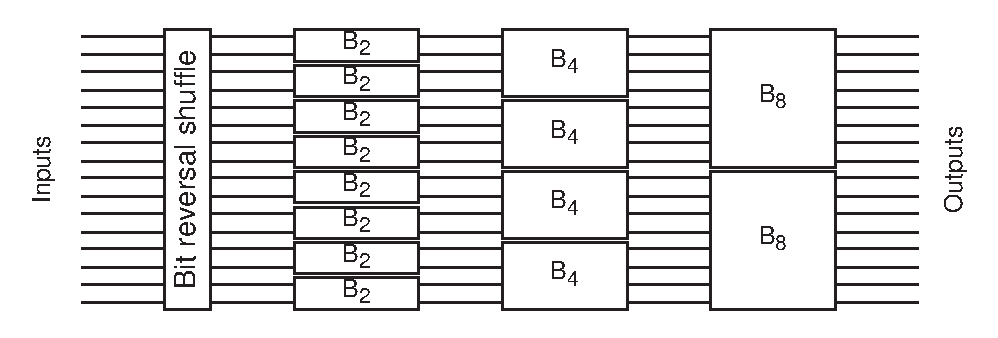
\includegraphics[width=11cm]{fftcomp}
\end{center}
\caption{FFT computation\label{Poly:FFTComp:Fig}}
\end{figure}

\smallskip
Although the algorithm described by \eqnref{FFT:Factor:Eq} appears to
be recursive, it turns out to be simpler if the column permutations
for all of the factors are performed at once.  The result is a single
reordering of the columns based on a very curious pattern.  Consider
what happens when
\eqnref{FFT:Factor:Eq} is applied twice to an $8\times8$ matrix.
Dealing only with the columns, we have
\[
A\Pi_8 = (A_0 \mid A_2 \mid A_4 \mid A_6 \mid A_1 \mid A_3 \mid A_5 \mid A_7).
\]
To apply \eqnref{FFT:Factor:Eq} to the copies of $\mathbf{F}_4$, we must
apply $\Pi_4$ to the first four columns and, separately, to the second
four columns, \ie,
\[
\begin{aligned}
(A_0 \mid A_2 \mid A_4 \mid A_6) \Pi_4 & = (A_0 \mid A_4 \mid A_2 \mid A_6),\\
(A_1 \mid A_3 \mid A_5 \mid A_7) \Pi_4 & = (A_1 \mid A_5 \mid A_3 \mid A_7),
\end{aligned}
\]
so
\[
A\Pi_8\Pi'_4 = 
  (A_0 \mid A_4 \mid A_2 \mid A_6 \mid A_1 \mid A_5 \mid A_3 \mid A_7).
\]
What has occurred is that we have sorted the columns, by the {\em bit
reversal} of their indexes.  This suggests a computational structure
as shown in \figref{Poly:FFTComp:Fig}.

\paragraph{Computational Framework}

Assume we have a vector of values $f^{(0)}_0, \ldots, f^{(0)}_{n-1}$
for which we want to compute the Fourier transform.  (We will use the
superscripts to indicate to which stage of the computation the value
corresponds.)  The first step is to reorder the $f_i$ by the bit
reversal of their indices, \ie, $f^{(1)}_i = f^{(0)}_{\mbox{rev}(i)}$,
where $\mbox{rev}(i)$ is the bit reversal of $i$.

The $f^{(1)}_i$ are now combined using a sequence of ``butterflies'' of
different sizes.  Each box in \figref{Poly:FFTComp:Fig} corresponds to
multiplication by the matrix
\[
B_r = \left(\begin{array}{cc} I_r & \Omega_r \\I_r & - \Omega_r
\end{array}\right),
\]
which we call a \keyi{butterfly}.  These matrices have precisely
two non-zero elements on each row.  Thus, when multiplying by $B_r$ we
have
\[
f^{(k+1)}_i \leftarrow f^{(k)}_i + \zeta f^{(k)}_{i+r}
\]
where $\zeta$ is an $n$-th root of unity.  It is convenient to
couple the computation of $f^{(k+1)}_i$ with that of
$f^{(k+1)}_{i+r}$:
\[
f^{(k+1)}_{i+r} \leftarrow f^{(k)}_i - \zeta f^{(k)}_{i+r}.
\]
We denote the pair of these computations by {\tt FFT2}:
\[
\mbox{\tt FFT2}[i, j, \zeta] \approx
\left\{
\left(\begin{array}{c} f^{(k+1)}_i \\ f^{(k+1)}_j \end{array}\right)
\leftarrow
\left(\begin{array}{cc} 1 & \zeta \\ 1 & -\zeta \end{array}\right)
\left(\begin{array}{c} f^{(k)}_i \\ f^{(k)}_j \end{array}\right)
\right\},
\]
where $\zeta$ is a root of unity.

The simplest computation is the 2 input butterfly, which consists of
just $\mbox{\tt FFT2}[2k, 2k+1, 1]$.  The four input butterfly
consists of two primitive computations:
\[
\mbox{\tt FFT2}[4k, 4k+2, \zeta_4^0], \mbox{\tt FFT2}[4k+1, 4k+3, \zeta_4^1],
\]
while the eight input butterfly consists of 
\[
\begin{array}{cc}
\mbox{\tt FFT2}[8k, 8k+4, \zeta_8^0],& 
  \quad \mbox{\tt FFT2}[8k+1, 8k+5, \zeta_8^1], \\
\mbox{\tt FFT2}[8k+2, 8k+6, \zeta_8^2],&
  \quad \mbox{\tt FFT2}[8k+3, 8k+7, \zeta_8^3].
\end{array}
\]

An implementation of the {\sc fft} consists of two parts: (1) a chunk of
code that shuffles the entries of $a_j$ to produce $a_j'$, and (2)
code that implements the sequence of butterflies.  In this discussion
we only discuss the second section.

The following routine replaces $f$ by its Fourier transform.  It
assumes that the length of $f$ is a power of $2$.
\begindsacode
FFT ($f$[n]) := $\{$ \\
\> FFT\=2 (i, j, $\zeta$) := $\{$ \\
\>\> $\left(\!\!\!\begin{array}{c}f\mbox{[i]}\\f\mbox{[j]}\end{array}\!\!\!\right)
  \leftarrow \left(\!\!\!\begin{array}{cc}1 & \zeta\\ 1 & -\zeta\end{array}\!\!\!\right)
  \left(\!\!\!\begin{array}{c}f\mbox{[i]}\\f\mbox{[j]}\end{array}\!\!\!\right)$;\\
\>\> $\}$; \\
\> FFT\=n (n, $k$) := $\{$ \\
\>\> unl\=ess $\mbox{n} = 2$ $\{$ \\
\>\>\> $\mbox{FFTn}(\mbox{n}/2, k)$;\\
\>\>\> $\mbox{FFTn}(\mbox{n}/2, k + \mbox{n}/2)$;\\
\>\>\> $\}$\\
\>\> loo\=p for $0 \le m < \mbox{n}/2$ do \{ \\
\>\>\> $\mbox{FFT2}(k+m, k+m+\mbox{n}/2, \zeta_{\mbox{m}})$; \\
\>\>\> $\}$ \\
\>\> $\}$ \\
\> $\mbox{FFTShuffle}(f)$; \\
\> $\mbox{FFTn}(\mbox{n}, 0)$; \\
\> $\}$
\enddsacode

\noindent
This routine uses two internal functions {\tt FFT2} and {\tt FFTn}.
{\tt FFT2} does 2 point butterfly.  The $n$ point butterfly is
implemented by the loop at the end of the {\tt FFTn}.  The first part
of {\tt FFTn} recursively computes the $n/2$ point butterflies.  

If we apply the Fourier transform and then the inverse Fourier
transform, as described by {\tt FFT}, to the same vector we will not
get the original vector, but $n$ times the original vector.  One
could deal with this problem either by adjusting the {\sc fft} routine
to remove a factor $\sqrt{n}$, or by removing a factor $n$ when
computing the inverse Fourier transform.

\medskip
One of the problems with the ``binary'' algorithm discussed in this
section is that the length of the vector transformed must be a power
of $2$.  In the years since the modern introduction of the {\sc fft}
algorithm \cite{Cooley1965-bp}, a vast number of extensions and variations
of the basic scheme discussed here have been developed.  Among these
variations are versions that permit the length of the algorithm to be
the product of small primes, \eg, $3^k$, and variations that merge the
argument shuffling we've used into the ``butterflies.''  Although all
of these methods asymptotically require $O(N \log N)$ operations, the
practical benefits they yield are very significant.

All of these {\sc fft} algorithms are valid over any field, $L$, that
contains $n$-th roots of unity.  If $L$ is either $\R$ or $\C$ then
$e^{2\pi i/n}$ can be used.  In this case, there are many good
libraries of {\sc fft} routines, including vectorized routines for
supercomputers \cite{Swarztrauber1984-zd,Bailey1988-ay,Bailey1988-rv}.  In the case
of $L = \R$ there are variants that encode two real numbers as a
single complex number thus decreasing the number stages in the {\sc fft} by
$1$.  It is also possible to combine two real valued vectors into a
single complex complex valued vector, also decreasing the number of
arithmetic operations by a factor 2. 

When $L$ is the rational integers, $\Z$, we can continue to use
$e^{2\pi i/n}$ as a primitive $n$-th root of unity\index{primitive root!of unity} if the round-off
errors introduced are carefully analyzed.  This is not the case when
$L$ is a finite field.  Assume that $L = \F_q$, so every element of
$L$ is a zero of $X^{q-1} - 1$, \ie, every element of $L$ is a root of
unity.  If $n$ divides $q-1$ then, by the discussion in
\sectref{FF:Multiplicative:Sec}, $L$ has $\phi(n)$ elements of order
$n$.  Each of these is a primitive $n$-th root of unity.   

If one needs an $n$-th root of unity that does not lie in $\F_q$,
then it can always be obtained by adjoining zeroes of irreducible
factors of $X^n-1$ to $\F_q$.  This however, can be quite expensive.
For instance, to interpolate a polynomial of degree $63$ over $\F_5$,
we need a $64$-th root of unity.  The smallest field of
characteristic $5$ with $64$-th roots of unity is $\F_{5^{16}}$.
Arithmetic in this field is at least $16 \log 16 = 64$ times more
expensive than arithmetic in $\F_5$.  So, the {\sc fft} approach here
is not likely to be of benefit.

\paragraph{FFT Based Interpolation}

The fast Fourier transform routine, {\tt FFT}, allows us to
interpolate the right type of black boxes exceedingly quickly.  Assume
that ${\cal B}_P$ represents a polynomial of degree $d$ over a field
$L$.  Let $n$ be $\lceil \log_2 d \rceil$ and assume that $\zeta \in
L$ is a primitive root of unity\index{primitive root!of unity} of
order $N = 2^n$.  Construct the set of values
\[
{\cal B}_P(1), {\cal B}_P(\zeta), {\cal B}_P(\zeta^2), {\cal
B}_P(\zeta^3), \ldots, {\cal B}_P(\zeta^{2^n-1}).
\]
The Fourier transform of this sequence will be the coefficients of
$P$.  The last $2^n - d$ of them should be zero.

The time required of this approach is $N = 2^{\lceil \log_2 d
\rceil}$ evaluations and $O(N \log N) = O(d \log d)$ operations for 
the {\sc fft}.

\medskip
It is informative to analyze the case of $L = \Z$ in a bit more
detail.  Assume that we are also given $B \ge |P|$, a bound on the
absolute value of the coefficients of $P$, in addition to $n$, a power
of two that bounds the degree of $P$.  Instead of performing the
interpolation over $\R$, we can instead choose a set of fields
$\F_{q_1}, \ldots, \F_{q_k}$, of characteristic $p_1, \ldots, p_k$
such that $n \mid (q_i -1)$ and such that $p_1 \cdots p_k \ge 2B + 1$.
Using $k \cdot n$ evaluations of ${\cal B}_P$ we can compute the image
of $P$ modulo the $p_i$.  The \key{Chinese remainder theorem} can now be
used to reconstruct $P$ over the integers.  The time required by such
an approach is
\[
O(k n \log n + n M_{\rm int}(\log B)^2)
\]
where $M_{\rm int}(\log B)$ is the time to multiply to integers of
$\log B$ bits.  Again this is asymptotically faster than the simpler,
Lagrangian and Newtonian interpolation algorithms discussed earlier,
but practically it is not of use except for univariate polynomials of
large degree.

\paragraph{Fast Polynomial Multiplication}

Let $F(X)$ and $G(X)$ be two polynomials over degree $m$ over a field
$L$,
\[
\begin{aligned}
  F(X) &= f_{m-1} X^{m-1} + f_{m-2} X^{m-2} + \cdots + f_0,\\
  G(X) &= g_{m-1} X^{m-1} + g_{m-2} X^{m-2} + \cdots + g_0.
\end{aligned}
\]
We want to compute $H(X) = F(X) G(X)$, were $\deg H = n = 2m$.  Using
classical multiplication we can do this using $O(n^2)$
multiplications.  We would like to do better using interpolation. 

We can easily construct a black box for $H$, ${\cal B}_H(x) = F(X)
G(x)$, when $x \in L$.  By choosing $n$ values of $x$ and using the
univariate interpolation techniques discussed earlier, we can
reconstruct $H$.  The cost however is still $O(n^2)$ multiplications.
Each evaluation of ${\cal B}_H$ requires $O(n)$ multiplications, so it
takes $O(n^2)$ multiplications to compute all of the values.  The
Newtonian and Lagrangian interpolation schemes themselves require
$O(n^2)$ operations.

However, by using the fast Fourier transform we can do better.  The
interpolation cost immediately drops from $O(n^2)$ to $O(n \log n)$.
In addition, we can compute all of the values of $F(X)$ and $G(X)$
using a single fast Fourier transform for each.  Thus we can bring the
total asymptotic cost of polynomial multiplication down to $O(n \log
n)$.  This technique for multiplying polynomials is the most efficient
known thus far.  However, all of the practical problems alluded to in
the previous section apply here also.  These problems are exacerbated
when dealing with multivariate polynomials, which frequently occur.

On the other hand, for moderate to large degree univariate polynomials
with coefficients in $\R$, $\C$, or, perhaps, small elements of $\Z$,
the {\sc fft} method can be quite effective.  When $L = \R$ this is
especially true if one uses an {\sc fft} routine that determines the
transform of two real functions at once using a single complex
transform.

\index{fast Fourier transform|)}


\section{Abstract Interpolation} 
\label{Interp:Abstract:Sec}

In this section we introduce a bit more abstraction into our
discussion of interpolation.  This will allow us to deal with a
variety of different types of interpolation problems in a uniform
framework.

Let $R$ be a commutative ring with unit and let $\mathfrak{m}$ be an
ideal of $R$.  Recall that $R/\mathfrak{m}$ is set of residue classes of
$R$ modulo $\mathfrak{m}$.  Two elements of $R$ $x$ and $y$ are in the
same equivalence class in $R/\mathfrak{m}$ if $x - y$ is an element of
the ideal $\mathfrak{m}$.  There is a natural map that sends elements of
$R$ to the equivalence classes in which they lie in $R/\mathfrak{m}$.
This map induces a ring structure on $R/\mathfrak{m}$.  If $\mathfrak{m}$ is
a \key{prime ideal} then $R/\mathfrak{m}$ is an \key{integral domain}.
If $\mathfrak{m}$ is a \key{maximal ideal} then $R/\mathfrak{m}$ is a field.

For many rings $R$ and ideals $\mathfrak{m}$ there is a canonical
representative for each class in $R/\mathfrak{m}$.  In such cases, we use
the canonical representative and the equivalence class
interchangeably.

Two common examples are $R = \Z$ and $R = L[X]$, where $L$ is a field.
The ideals of $\Z$ are principal, \ie, all ideals are generated by a
single element, $\mathfrak{m} = (m)$.  The canonical representatives of
the equivalence classes of the quotient ring $\Z/(m)$ are the integers
$\{0, 1, \ldots, m-1\}$ (using the \key{one sided presentation} of
\chapref{Finite:Fields:Chap}).  The prime ideals of $\Z$ are also
maximal.  If $m$ is prime them $\Z/(m)$ is a field.  If on the
other hand, $m$ is divisible by $p > 1$, then $p$ will be a zero
divisor and $Z/(m)$ cannot be an integral domain.

The ideals of $L[X]$ are also principal, but are generated by the
polynomials in $L[X]$.  Let $\mathfrak{m} = (m(X))$ be an ideal in
$L[X]$.  Since $L$ is a field, we can assume that $m(X)$ is monic.  As
with $\Z$, the canonical representatives in $L[X]/\mathfrak{m}$ are the
reduced residues modulo $m(X)$.  The case when $m(X)$ is linear occurs
frequently.  Let $a(X) \in L[X]$ be a polynomial, and assume $m(X) = X
- k$, where $k$ is an element of $L$.  The remainder of $a(X)$ when
divided by $X - k$ is $a(k)$.

For $a$ an element of a ring $R$, and $\mathfrak{m}$ an ideal of $R$, we
use the notation
\[
a(\mathfrak{m}) = a \mod\mathfrak{m}.
\]
Thus, if $\mathfrak{m} = (X - k)$ then $a(k) = a(\mathfrak{m}) = a((X -
k))$.  Note the extra set of parenthesis in the last form, which will
not be often used.  

\medskip
With this notation we can discuss interpolation in a manner that
strengthens the parallels between the Chinese remainder algorithm for
integers of \sectref{Integer:Chinese:Remainder:Sec} and that for
polynomials in \sectref{Interp:CRA:Sec}.  The following is the
standard version of the \key{Chinese remainder theorem}

\begin{proposition}[Chinese Remainder Theorem]
Let $\mathfrak{p}_1, \ldots, \mathfrak{p}_n$ be ideals in a ring $R$, such
that every pair is co-prime, \ie, $\mathfrak{p}_i + \mathfrak{p}_j = (1)$ if
$i\not=j$.  There is a one to one correspondence between $n$-tuples in
$R/\mathfrak{p}_1 \times \cdots \times R/\mathfrak{p}_n$ and $R/\mathfrak{p}_1
\cdots \mathfrak{p}_n$.
\end{proposition}

Let $\mathfrak{p}_1, \ldots, \mathfrak{p}_t$ be ideals in $R$ and $F$
be an element of $R$.  The interpolation problem is: Given
$F(\mathfrak{p}_1), \ldots, F(\mathfrak{p}_t)$ compute an element of
$R/\mathfrak{p}_1 \cdots \mathfrak{p}_t$ whose image in
$R/\mathfrak{p}_i$ is $F(\mathfrak{p}_i)$.  In the context of black
boxes, we have a black box ${\cal B}_F$ that accepts an ideal
$\mathfrak{q}$ and returns ${\cal B}_F(\mathfrak{q}) = F(\mathfrak{q})$.
Again our goal is reconstruct $F$.

Consider the simple case where there are only two ideals $\mathfrak{p}$
and $\mathfrak{q}$.  We are given $F(\mathfrak{p})$ and $F(\mathfrak{q})$ and
we want to compute $F(\mathfrak{pq})$.  Recall that when $R = \Z$ it was
necessary to require that the two moduli be relatively prime.  With
ideals, the same constraint is that $\mathfrak{p} + \mathfrak{q} = 1$.  That
is, there exist $a \in \mathfrak{p}$ and $b \in \mathfrak{q}$ such that
$a+b=1$.  Thus
\[
F(\mathfrak{pq}) = a F(\mathfrak{p}) + b F (\mathfrak{q}).
\]

In more generality, let $\mathfrak{p}_1, \ldots, \mathfrak{p}_t$ be pairwise
co-prime ideals in $R$ and define
\[
\mathfrak{P}_i = \mathfrak{p}_1 \cdots \mathfrak{p}_{i-1} \mathfrak{p}_{i+1}
\cdots \mathfrak{p}_t.
\]
The $\mathfrak{P}_i$ are defined so that 
\[
\mathfrak{P}_1 + \mathfrak{P}_2 + \cdots + \mathfrak{P}_t = (1)
\]
any smaller subset is divisible by some $\mathfrak{p}_j$.  Letting $p_i$
be elements of $\mathfrak{P}_i$ whose sum is $1$ gives,
\begin{equation}\label{CRA:Lagrange:Eq}
F(\mathfrak{p}_1 \cdots \mathfrak{p}_t) = 
 p_1 F(\mathfrak{p}_1) + p_2 F(\mathfrak{p}_2) + \cdots +
  p_t F(\mathfrak{p}_t).
\end{equation}

When $R = k[Z]$ this is precisely the \key{Lagrange interpolation
formula} discussed earlier.  Let $\mathfrak{p}_i = (Z - z_i)$, so
\[
\mathfrak{P}_i = \left((Z - z_0) \cdots (Z-z_{i-1})(Z-z_{i+1}) \cdots
(Z-z_t)\right)
\]
and
\[
p_i = \frac{(Z-z_0)\cdots(Z - z_{i-1})(Z - z_{i+1}) \cdots (Z-z_t)}{(z_i-z_0)\cdots(z_i - z_{i-1})(z_i - z_{i+1}) \cdots (z_i-z_t)}.
\]
The sum of the $p_i$ is a polynomial of degree $t$.  Its value at $Z =
z_0, z_1, \ldots, z_t$ is $1$ so it must be identically equal to $1$.

A Lagrangian interpolation formula can be developed for $R = \Z$ by
using \eqnref{CRA:Lagrange:Eq}.  Consider the simple case of two
ideals, $\mathfrak{p} = (p)$ and $\mathfrak{q} = (q)$.  Again, we are
looking for $a \in \mathfrak{p}$ and $b \in \mathfrak{q}$ such that $a+b =
1$ modulo $\mathfrak{pq}$.  Since  $a = xp$ and $b = yq$, we want to find
$x$ and $y$ such that 
\begin{equation} \label{Abs:Dio:Eq}
xp + yq = 1,
\end{equation}
where $x$ and $y$ are integers.  As we know this diophantine equation
has solutions if and only if $p$ and $q$ are relatively prime.  Let
$\bar{x}$ and $\bar{y}$ be solutions of \eqnref{Abs:Dio:Eq}.

If we have
\[
\begin{aligned}
F &= k_1 \pmod{p} \\
F &= k_2 \pmod{q}
\end{aligned}
\]
Then a Lagrangian interpolation formula for $F$ is
\[
F = \bar{x} \cdot  k_2 \cdot p + \bar{y} \cdot k_1 \cdot q \pmod{pq}.
\]

\section*{Notes}

\small

\notesectref{Vandermonde:Sec} \propref{Gen:Vandermonde:Prop} appears
in {\Polya} and {\Szego} \cite{Polya1978-hx}, Chapter 5, problem 48.
Additional partial results on generalized Vandermonde matrices are
contained in the work of {\MitchellO} \cite{Mitchell1881-cv}, and
{\EvansR} and {\Isaacs} \cite{Evans1976-dq}.

\notesectref{Poly:FFT:Sec}
The fast Fourier transform algorithm was first discussed in modern
terms by {\Cooley} and {\Tukey} \cite{Cooley1965-bp}, although the basic
ideas have been known by a variety of authors starting with {\Gauss}.
See \cite{Heideman1984-zr} for a historical survey.  More detailed
discussions of fast Fourier transform algorithms and their
applications are contained in 
\cite{Tolimieri1989-sz,Brigham1988-dw,Van_Loan1992-cb,Pollard1971-qy}.

{\CantorD} and {\Kaltofen} \cite{Cantor1991-rr} have generalized the {\sc fft}
polynomial multiplication technique to polynomials over arbitrary
algebras.  For univariate polynomials of degree $n$, their technique
requires $O(n \log n)$ multiplies and $O(n \log n \log \log n)$
additions.

Bonneau has studied the use of {\sc fft} to speed polynomial
multiplication
\cite{Bonneau1974-if}.

\normalsize

    %$Id: interp.tex,v 1.1 1992/05/10 19:42:22 rz Exp rz $
\chapter{Multivariate Interpolation}
\label{Sparse:Interp:Chap}

Multivariate polynomial interpolation is a bit more complex than the
univariate interpolation techniques discussed in
\chapref{Interpolation:Chap}.  Because the number of possible terms in
a multivariate polynomial can be exponential in the number of
variables, techniques similar to those of \chapref{Zero:Testing:Chap}
must be used to avoid spending inordinate amounts of time computing
coefficients that are equal to zero.

\sectref{Interp:MDense:Sec} demonstrates how
the univariate interpolation schemes recursively give a
deterministic multivariate algorithm that takes time $O(d^v)$ to 
reconstruct a polynomial in $v$ variables of degree no more than $d$ in 
each from its values.  For dense polynomials, where the number of 
non-zero terms is $O(d^n)$, this is an efficient algorithm.  
\sectref{Interp:PSparse:Sec} gives a probabilistic interpolation algorithm that
takes $O(T^3)$ time to compute such a polynomial with $T$ non-zero terms 
from its values.  For practical 
implementations this appears to be the most efficient interpolation
algorithm for sparse polynomials.  In \sectref{Interp:ZSparse:Sec} we
demonstrate how this algorithm can be made deterministic.

\sectref{Interp:BenOr:Sec} presents a different interpolation scheme
that, unlike the algorithm of \sectref{Interp:ZSparse:Sec}, does not
require a bound on the degrees of the variables in $P$.
Theoretically, this algorithm has better performance than the
algorithm of \sectref{Interp:ZSparse:Sec}, but from a practical point
of view the probabilistic approach is preferable.


\section{Multivariate Dense Interpolation}
\label{Interp:MDense:Sec}

As pointed out in \chapref{Interpolation:Chap}, a polynomial in one variable
of degree $d$ can be determined from its values at $d+1$ points using
$O(d^2)$ arithmetic operations.  This result can be extended to
multivariate problems recursively.

Assume we are given a black box ${\cal B}_P$ for the polynomial
$P(X_1, \ldots, X_n)$ with a degree bound, $\deg_{X_i} P = d$.  
We can assume that $P$ has the form
\[
P(X_1, \ldots, X_n) = P_0(X_2, \ldots, X_n) X_1^d + 
\cdots + P_d(X_2, \ldots, X_n).
\]
Using the univariate interpolation schemes of the previous chapter
we can create black boxes ${\cal B}_{P_0}, \ldots, {\cal B}_{P_d}$, for
the $n-1$-variate coefficients of $P$ as follows:

To find the value of ${\cal B}_{P_i}(x_{20}, \ldots, x_{n0})$, choose
a sequence of $d+1$ different evaluations, points where the first
component is chosen at random and the last $n-1$ components are
$x_{20}, \ldots, x_{n0}$.  Applying the interpolation algorithms of
the last chapter, we can compute $P(X_1, x_{20}, \ldots, x_{n0})$:
\[
\left.
\begin{array}{c}
{\cal B}_P(x_{10}, x_{20}, \ldots, x_{n0}) \\ \vdots \\
{\cal B}_P(x_{1,d+1}, x_{20}, \ldots, x_{n0})
\end{array} \right\} \longrightarrow P(X_1, x_{20}, \ldots, x_{n0}).
\]
The coefficients of this polynomial are
\[
\begin{aligned}
P(X_1, x_{20}, \ldots, x_{n0}) 
   & = P_0(x_{20}, \ldots, x_{n0}) X_1^d + \cdots + P_d(x_{20}, \ldots, x_{n0}), \\
   & = {\cal B}_{P_0}(x_{20}, \ldots, x_{n0}) X_1^d + \cdots 
     + {\cal B}_{P_d}(x_{20}, \ldots, x_{n0}).
\end{aligned}
\]
So at the cost of $d+1$ evaluations, we can determine one value of
each of the $d+1$ black boxes, ${\cal B}_{P_0}, \ldots, {\cal B}_{P_d}$. 

This process is then repeated, but with a different value for the $X_2$
coordinate,
\[
\left.
\begin{array}{c}
{\cal B}_P(x_{10}, x_{21}, x_{30}, \ldots, x_{n0}) \\ \vdots \\
{\cal B}_P(x_{1,d+1}, x_{21}, x_{30}, \ldots, x_{n0})
\end{array} \right\} \longrightarrow P(X_1, x_{21}, x_{30}, \ldots, x_{n0}),
\]
which gives another value for each of the ${\cal B}_{P_i}$.  When
repeated $d+1$ times, $P(X_1, X_2, x_{30}, \ldots, x_{n0})$ can be
reconstructed as shown in \figref{SI:DenseAlg:Fig}

\begin{figure}
\small
\[
\hspace*{-14pt}\left.
\begin{array}{c}
\left.
\begin{array}{c}
{\cal B}_P(x_{10}, x_{20}, \ldots, x_{n0}) \\ \vdots \\
{\cal B}_P(x_{1,d+1}, x_{20}, \ldots, x_{n0})
\end{array} \right\} \rightarrow P(X_1, x_{20}, \ldots, x_{n0})\\
\vdots \\
\left.
\begin{array}{c}
{\cal B}_P(x_{10}, x_{2d}, \ldots, x_{n0}) \\ \vdots \\
{\cal B}_P(x_{1,d+1}, x_{2d}, \ldots, x_{n0})
\end{array} \right\} \rightarrow P(X_1, x_{2d}, \ldots, x_{n0})
\end{array} \right\}
\rightarrow P(X_1, X_2, x_{30}, \ldots, x_{n0})
\]
\normalsize
\caption{Dense Interpolation Scheme\label{SI:DenseAlg:Fig}}
\end{figure}

This recursive process can now be repeated with the $(d+1)^2$
coefficients $P(X_1, X_2, x_{30}, \ldots, x_{n0})$.  Each set of
coefficient values can be computed with $(d+1)^2$ values.  More
generally, the $(d+1)^k$ coefficients of $P(X_1, \ldots, X_k,
x_{k+1,0}, \ldots, x_{n0})$ can be computed with $(d+1)^k$ evaluations
of ${\cal B}_P$.  And thus $P(X_1, \ldots, X_n)$ can be determined
with $(d+1)^k$ values.

To analyze the complexity of this algorithm, let $I(d)$ denote the
time complexity of interpolating $d+1$ values to produce a univariate
polynomial of degree $d$.  And let $N_k$ be the complexity of the
previous algorithm for $k$ variables.  We have
\[
\begin{aligned}
N_1 & = I(d), \\
N_2 & = (d + 1) N_1 + (d+1)I(d), \\
& \vdots \\
N_k & = (d+1) N_{k-1} + (d+1)^{k-1} I(d).
\end{aligned}
\]
It is easy to show by induction that the solution to this recurrence
is
\[
N_k = k(d+1)^{k-1} I(d).
\]
Using a classical interpolation algorithm, $I(d) = O(d^2)$, so this
algorithm requires $O(n d^{n+1})$ operations.  Using evaluation points
that satisfy the requirements of the \key{fast Fourier transform}
reduces this cost to $O(n d^n \log d)$.

\section{Probabilistic Sparse Interpolation}
\label{Interp:PSparse:Sec}

This section develops the sparse interpolation algorithm
\cite{Zippel1990-ab}, which uses probabilistic techniques to interpolate a 
polynomial in time dependent on the number of non-zero terms.  This 
algorithm is given no information about the number of non-zero terms in 
the polynomial being interpolated. Instead it develops an estimate of the 
number of terms as each new variable is introduced.  As a consequence its 
performance depends upon the actual number of non-zero terms in the 
polynomial rather than an {\em a priori} bound.  For most practical 
problems, this appears to be the best algorithm available and tends to be 
more useful than the deterministic algorithms presented in the following 
sections \cite{Manocha1991-iq}.

This section has three parts.  The first demonstrates the sparse 
interpolation algorithm via an example. The next part gives a formal 
specification of the algorithm, while the final part analyzes the 
algorithm's performance. 

\paragraph{Heuristic Presentation}

As before, we wish to determine the polynomial $P(\vec X) \in L[\vec
X]$ from a black box ${\cal B}_P$, where $L$ is a field with
sufficiently many distinct elements.  We assume that $D$ bounds the
degree of $X_i$ in $P$.  The sparse interpolation algorithm computes
$P$ one variable at a time.  That is, we initially compute $P(a_1,
a_2, \ldots, a_n)$, then $P(X_1, a_2, \ldots,a_n)$, then $P(X_1, X_2,
a_3, \ldots, a_n)$ and so on, until we have determined $P(\vec X)$.
The introduction of each new variable is called a {\em stage} of the
algorithm.\index{stage!of interpolation algorithm}  We use clues from the 
polynomial produced in the preceding stage to minimize the effort 
required to produce the next polynomial in the sequence. 

The formal description of the sparse interpolation algorithm is rather
involved and it is easy to get bogged down by all the subscripts and
variables involved.  Nonetheless, the basic ideas behind the sparse
interpolation algorithm are fundamentally quite simple, as the
following example illustrates.

Let ${\cal B}_P$ be a black box representing the polynomial
\[
P(X, Y, Z) = 
  X^5 Z^2 + X^5 Z + X Y^4 + X Y Z^5 + Y^5 Z.
\]
We are given a degree bound of $5$ for each variable, so there are
$(5+1)^3 = 216$ different coefficients that need to be determined.
Given no other information, any deterministic interpolation scheme
would require $216$ calls to ${\cal B}_P$.  

Using either \keyw{LagrangeInterp} or \keyw{NewtonInterp}, the values
\[
{\cal B}_P(x_0, y_0, z_0), {\cal B}_P(x_1, y_0, z_0), \ldots, 
{\cal B}_P(x_5, y_0, z_0).
\]
can be interpolated to produce the polynomial:
\[
P(X, y_0, z_0) = c_0 X^5 + c_1 X + c_2.
\]
Having introduced the first variable, we have completed the first
stage.

The purpose of the second stage is to determine $P(X, Y, z_0)$.  The
dense interpolation scheme repeats the process of the previous
paragraph, using $6$ different evaluation points, to produce $P(X,
y_1, z_0)$.  The sparse interpolation scheme recognizes that $P(X,y_1,
z_0)$ probably only has $3$ non-zero coefficients and most likely has
the form
\[
P(X, y_1, z_0) = c_3 X^5 + c_4 X + c_5.
\]
Since there are only three unknown coefficients in $P(X, y_1, z_0)$,
only $3$ different values of ${\cal B}_P$ are needed to determine
them.  The overall computation of $P(X, Y, z_0)$ is shown in 
\figref{SI:SparseAlg:Fig}
\begin{figure}
\small
\[
\hspace*{-1pt}\left.\begin{array}{c}
\left.\begin{array}{c}
{\cal B}_P(x_0, y_0, z_0) \\ \vdots \\ {\cal B}_P(x_5, y_0, z_0)
\end{array}\right\} \rightarrow c_0X^5 + c_1 X + c_2 \\
\left.\begin{array}{c}
{\cal B}_P(x_0, y_1, z_0) \\ {\cal B}_P(x_1, y_1, z_0) \\ 
{\cal B}_P(x_2, y_1, z_0)
\end{array}\right\} \rightarrow c_3X^5 + c_4 X + c_5 \\
\vdots \\
\left.\begin{array}{c}
{\cal B}_P(x_0, y_5, z_0) \\ {\cal B}_P(x_1, y_5, z_0) \\ 
{\cal B}_P(x_2, y_5, z_0)
\end{array}\right\} \rightarrow c_{15}X^5 + c_{16} X + c_{17} 
\end{array}\right\} \rightarrow d_0 X^5 + (d_1 Y^4 + d_2 Y) X + d_3 Y^5
\]
\normalsize
\caption{Sparse Interpolation Scheme\label{SI:SparseAlg:Fig}}
\end{figure}

After the $6$ different univariate polynomials, $P(X, y_i, z_0)$ are
computed, their coefficients are interpolated to produce $P(X, Y,
z_0)$.  Notice that only $6 + 5 \times 3 = 21$ evaluations are needed
so far, while the dense interpolation scheme requires $36$.

The third stage proceeds in the same fashion, but with even greater
savings.  We want to compute the six polynomials
\[
P(X, Y, z_i) = d_{4i} X^5 Z + d_{4i+1} X Y^4 + d_{4i+2} X Y + d_{4i+3} Y^5,
\]
for $i = 0, \ldots, 5$.  $P(X, Y, z_0)$ is known from the second
stage, and we assume that all of the $P(X, Y, z_i)$ have the same skeleton
as $P(X, Y, z_0)$.

Since there are only four unknowns in $P(X, Y, z_i)$, each set of the
$d_i$'s can be determined using only four values from ${\cal B}_P$ and
solving the resulting system of linear equations.  These equations can
be solved in $O(N^3)$ time using classical Gaussian elimination.
Notice that this approach places absolutely no restrictions on the
values used for the interpolation points.  This is quite useful in
certain problems where the user of the interpolation algorithm has its
own restrictions to place on the evaluation points \cite{Rubinfeld1994-lq}.

However, if the interpolation algorithm is free to choose the
evaluation points then the $O(N^3)$ Gaussian elimination cost can be
reduced to $O(N^2)$ by choosing the values for $X$ and $Y$ so that the
system of equations be a transposed Vandermonde
system.\index{Vandermonde system!transposed} Consider, for instance,
the computation of $P(X,Y,z_1)$.  For randomly chosen $x_{\alpha}$ and
$y_{\alpha}$ compute the four values
\[
\{P(1,1,z_1), P(x_{\alpha},y_{\alpha},z_1),
  P(x_{\alpha}^2,y_{\alpha}^2,z_1),
  P(x_{\alpha}^3,y_{\alpha}^3,z_1) \}.
\]
This gives the following Vandermonde system of equations for $d_4$,
$d_5$, $d_6$ and $d_7$:
\[
\begin{aligned}
d_4 (x_{\alpha}^5)^0 + d_5 (x_{\alpha} y_{\alpha}^4)^0 +
  d_6 (x_{\alpha} y_{\alpha})^0 + d_7 (y_{\alpha}^5)^0
    & = {\cal B}_P(1,1,z_1), \\
d_4 (x_{\alpha}^5)^1 + d_5 (x_{\alpha} y_{\alpha}^4)^1 +
  d_6 (x_{\alpha} y_{\alpha})^1 + d_7 (y_{\alpha}^5)^1
    & = {\cal B}_P(x_{\alpha},y_{\alpha},z_1), \\
d_4 (x_{\alpha}^5)^2 + d_5 (x_{\alpha} y_{\alpha}^4)^2 +
  d_6 (x_{\alpha} y_{\alpha})^2 + d_7 (y_{\alpha}^5)^2
    & = {\cal B}_P(x_{\alpha}^2,y_{\alpha}^2,z_1), \\
d_4 (x_{\alpha}^5)^3 + d_5 (x_{\alpha} y_{\alpha}^4)^3 +
  d_6 (x_{\alpha} y_{\alpha})^3 + d_7 (y_{\alpha}^5)^3
    & = {\cal B}_P(x_{\alpha}^3,y_{\alpha}^3,z_1).
\end{aligned}
\]

Regardless of how the system of equations is created and solved, the 
computation of $P(X, Y, z_1)$ only requires $4$ values from ${\cal B}_P$,
rather than the $36$ values that a dense interpolation scheme 
requires.  $P(X, Y, z_2)$ through $P(X, Y, z_5)$ can be computed in the
same fashion.  Finally, the coefficients of these polynomials can be
interpolated using a univariate interpolation scheme to get $P(X, Y, Z)$.
The total number of evaluations performed is $6 + 5 \times 3 + 5
\times 4 = 41$, which is a substantial improvement over the $216$
evaluations required by the dense interpolation.

For interpolation problems with more variables, the same recursive
structure is repeated. 

\paragraph{Formal Presentation}

To fix our notation, assume we want to determine a sparse polynomial
$P(X_1, \ldots, X_n) \in L[\vec X]$ where $L$ is a field.  The degree
of each $X_i$ in $P$ is bounded by $d$ and there are no more than $T$
non-zero monomials in $P$, \ie,
\[
P(X_1, \ldots, X_n) = c_1 \vec{X}^{\vec{e}_1} + c_2 \vec{X}^{\vec{e}_2} +
\cdots + c_T \vec{X}^{\vec{e}_T}.
\]
We assume that we are given a black box ${\cal B}_P$ that returns 
$P(\vec{x})$ when given a vector of values $\vec{x}$.  The set of 
exponents of a polynomial is called its {\em skeleton},\index{skeleton!of 
a polynomial} \ie{}  \addsymbol{$\skel P$}{The skeleton of a polynomial} 
\[
\skel P = \{\vec{e}_1, \vec{e}_2, \ldots, \vec{e}_T \}.
\]
We denote the {\em projection of the skeleton}\index{skeleton!projection 
of} of $P$ to $X_1, \ldots,
X_k$, by $\skel_k P$ defined by 
\addsymbol{$\skel_k P$}{Projection of the skeleton of a polynomial to
the first $k$ variables}
\[
\skel_k P = \{\, (e_1, \ldots, e_k) \mid \exists \vec{e}\in \skel P \,.\,
   \vec{e} = (e_1, e_2, \ldots, e_k, \ldots)\,\}
\]
So $\skel_k P$ is the set of tuples consisting of the first $k$ components
of elements of $\skel P$.  Notice that for all  $x_{k+1}, \ldots,
x_n \in L$, 
\[
\skel P(X_1, \ldots, X_k, x_{k+1}, \ldots, x_n) 
\subseteq \skel_k P(X_1, \ldots, X_n).
\]
Equality almost always occurs, but it is not necessary.  For instance, let
$P(X_1, X_2)$ be the polynomial $X_1^2 + X_1 X_2 + X_1$.  Then 
\[
\begin{aligned}
\skel P(X_1, X_2) &= \{(2, 0), (1, 1) (1, 0)\}, \\
\skel_1 P(X_1, X_2) & = \{ (2), (1) \}, \\
\skel P(X_1, -1) & = \{ (2) \}.
\end{aligned}
\]

We say that $(x_1, \ldots, x_n)$ is a \keyi{precise evaluation point}
if 
\[
\skel P(X_1, \ldots, X_k, x_{k+1}, \ldots, x_n) 
= \skel_k P(X_1, \ldots, X_n).
\]
for all $k > 1$.  Otherwise, $(x_1, \ldots, x_n)$ is said to be an
\keyi{imprecise evaluation point}.  The results of 
\sectref{Interp:MDense:Sec} allow us to estimate the likelihood of 
imprecise evaluation points as follows.

\begin{proposition}\label{Imprecise:Prob:Prop}
Let $P(X_1, \ldots, X_n)$ be a polynomial over an integral domain $A$.
Assume $\deg_{X_i} P \le D$ and $\terms P = T$.  Let ${\cal S}$ be a
subset of $A$ of cardinality $B$.  Then the probability that $(x_1,
\ldots, x_n)$ is an imprecise evaluation point of $P$, $x_i \in S$ is
bounded above by
\[
\frac{n(n-1)D T}{2B}.
\]
\end{proposition}

\begin{proof}
For each $k$ we can write
\[
P(X_1, \ldots, X_n) = c_{1k}(X_{k+1}, \ldots, X_n) \vec{X}^{\vec{f}_{1k}}
+ \cdots +
c_{Tk}(X_{k+1}, \ldots, X_n) \vec{X}^{\vec{f}_{Tk}},
\]
where $f_{ik} \in \skel_k P$.  In order for $\vec{x}$ to be
an imprecise evaluation point, it must be the zero of one of the
$c_{ij}$.  We can add up the probabilities, variable by variable.  By
\longpropref{Zero:MPoly:Prop}, the probability that $\vec{x}$ will be
a zero of one of $c_{1k}, \ldots, c_{Tk}$ is no more than
\[
\frac{(n-k)dT}{B}.
\]
Summing these probabilities gives
\[
\frac{(n-1)dT}{B} + \frac{(n-2)dT}{B} + \cdots + \frac{dT}{B} =
\frac{n(n-1)dT}{2B}.
\]
\end{proof}

\medskip

For exposition purposes, we consider one stage of the interpolation.
Assume we have performed the first $k-1$ stages of the sparse interpolation
algorithm and are about to begin the $k$-th stage.  Throughout the
$k$-th stage, the values assigned to $X_{k+1}, \ldots, X_{n}$ do
not vary.  To simplify the notation, we omit them\footnote{In an
implementation this may be more than notational.  Eliminating the
variables that do not vary at this stage can save significant time
when computing the values of $P$.} and write
\[
P'(x_0, \ldots, x_k) = P(x_1, \ldots, x_k, x_{k+1,0}, \ldots, x_{n0}).
\]
From the $k-1$-th stage's computation we have
\[
P(X_1, \ldots, X_{k-1}, x_{k0}, \ldots, x_{n0}) = p_{10} {\vec X}^{\vec e_1} +
p_{20} {\vec X}^{\vec e_2} + \cdots + p_{T0} {\vec X}^{\vec e_T}.
\]
We now assume that $\skel_k P = \{\vec{e}_1, \ldots, \vec{e}_T\}$,
\ie, $(x_{10}, \ldots, x_{n0})$ is a precise evaluation point for $P$.
This is the probabilistic assumption that underlies the algorithm.

The computation of $P(X_1, \ldots, X_{k-1}, X_k)$ proceeds in two phases: 
First, we determine  
\[
P'(X_1, \ldots, X_{k-1}, x_{kj}) = 
p_{1j} {\vec X}^{\vec e_1} + p_{2j} {\vec X}^{\vec e_2} + \cdots + p_{Tj} {\vec
X}^{\vec e_T},
\]
for $j = 1, \ldots, n$ by the following technique:

For randomly chosen $x_{kj}$ perform the following: Pick a $k-1$-tuple
denoted by $(y_1, \ldots, y_{k-1}) = \vec y$, such that each of $m_i =
{\vec y}^{\vec e_i}$ are distinct. Since the ${\vec e_i}$ are known,
verifying that this is the case is easy.  This value allows
us to set up the following (non-singular) transposed
Vandermonde system\index{Vandermonde system!transposed} of linear equations
\begin{equation}
 \label{SPMod:Vandermonde:System:Eq}
\begin{aligned}
  P'(1, \ldots, 1, x_{k,1})
    &= p_{1j} + p_{2j} + \cdots + p_{Tj}, \\
  P'(y_1, \ldots, y_{k-1}, x_{kj})
    &= p_{1j} {\vec y}^{\vec e_1} + p_{2j} {\vec y}^{\vec e_2} + \cdots +
      p_{Tj} {\vec y}^{\vec e_T}, \\
  P'(y_1^2, \ldots, y_{k-1}^2, x_{kj})
    &= p_{1j} {\vec y}^{2\vec e_1} + p_{2j} {\vec y}^{2\vec e_2} + \cdots +
      p_{Tj} {\vec y}^{2 \vec e_T}, \\
    &\vdots\\
  P'(y_1^T, \ldots, y_{k-1}^T, x_{kj})
    &= p_{1j} {\vec y}^{T \vec e_1} + p_{2j} {\vec y}^{T \vec e_2} + \cdots
      + p_{Tj} {\vec y}^{T \vec e_T},
\end{aligned}
\end{equation}
which can be solved by the techniques of \sectref{Vandermonde:Sec} in
$O(T^2)$ time and $O(T)$ space.  The result is a polynomial
\[
P'(X_1, \ldots, X_{k-1}, x_{kj}),
\]
for each of $d$ values $x_{kj}$. 

Second, we independently interpolate the coefficients of each
monomial, using the dense interpolation algorithm.  The results of these
interpolations are combined to produce
\[
P'(X_1, \ldots, X_{k-1}, X_k) 
  = p_1(X_k) {\vec X}^{\vec e_1} + p_2(X_k) {\vec X}^{\vec e_2} 
     + \cdots + p_T(X_k) {\vec X}^{\vec e_T}.
\]
The dense interpolation yielded the univariate polynomials $p_i(X_k)$.
The $p_i(X)$ are in turn expanded to get:
\[
P(X_1, \ldots, X_{k}, x_{k+1,0},\ldots, x_{n0}) 
  = p_{10}' {\vec X}^{\vec e_1'} + p_{20}' {\vec X}^{\vec e_2'} 
    + \cdots + p_{T0}' {\vec X}^{\vec e_T'}.
\]
This is the value returned by the $k$-th stage.  We are ready to
begin lifting the next variable.

\medskip
The routine \keyw{SparseInterpStage} below implements this approach.
Its arguments are a $k-1$ variable polynomial that results from the
$k-1${\st} stage, a black box representing the polynomial $P(X_1,
\ldots, X_k)$, a bound on the degree of $X_k$ in $P$ and $k$.  Within
{\tt SparseInterpStage} we have used $L$ to denote the coefficient
domain of $P$.  \Marginpar{In the following fix the skeleton if
$P_{k-1}$ is zero.}

\begindsacode
SparseInterpStage ($P_{k-1}$, ${\cal B}_P$, $D$, $k$) := $\{$ \\
\> $S \leftarrow \skel P_{k-1}$; \\
\> $\ell \leftarrow \mbox{length}(S)$; \\
\> $\vec{y} \leftarrow \mbox{InitY}(L, k - 1)$; \\
\> $m[\cdot] \leftarrow \vec{y}^S$; \\
\> loo\=p for $1 \le i \le D$ do $\{$ \\
\>\> $x[i] \leftarrow \mbox{random}(L^{k-1})$; \\
\>\> $B \leftarrow \{{\cal B}_P(\vec{y}^0, x[i]), \ldots, 
  {\cal B}_P(\vec{y}^{\ell}, x[i])\}$; \\
\>\> $\mbox{\em Eq}[i, \cdot] \leftarrow \mbox{SolveVandermondeT}(m[\cdot], B[\cdot])$;\\
\>\> $\}$ \\
\> $P_k \leftarrow 0$; \\
\> loo\=p for $i \le j < \ell$ do $\{$\\
\>\> $P_k \leftarrow p_k + X^{S[j]} \cdot \mbox{NewtonInterp}(\mbox{\em Eq}[\cdot,
j], x[\cdot])$;\\
\>\> $\}$ \\
\> $\mbox{return}(P_k)$; \\
\> $\}$
\enddsacode

\noindent
The routine \keyw{InitY} provides the initial vector for $\vec{y}$.
{\tt InitY} needs to return values such that the $m_i =
\vec{y}^{\vec{e}_i}$ are distinct and thus the Vandermonde system will
be non-singular.\Marginpar{Explain what should be used in a practical
implementation, and what if $P_k{-1}=)$ above.}

If the coefficient domain is an integral domain of either
characteristic zero or sufficiently large finite characteristic then
this can easily be done.  When the characteristic of $L$ is zero
the image of $\Z$ in $L$ is isomorphic to
$\Z$.  \keyw{InitY} returns a vector consisting of the first $k-1$
rational primes, \ie, $2, 3, 5, 7, \ldots$.  By unique factorization
of elements of $\Z$ the $m_i$ must be distinct.  If the characteristic
of $L$ is finite, then the characteristic of $L$ must be larger than 
\begin{equation} \label{SI:FFBound:Eq}
(2 \cdot 3 \cdots p_n)^d \approx n^{c_1 nd}.
\end{equation}
to guarantee the $m_i$ are distinct.  In either case, the size of the
numbers involved in the interpolation are polynomial in the number
of variables and their degrees in the polynomial.

When the characteristic of $L$ is not larger than \eqnref{SI:FFBound:Eq} 
the problem of keeping the \key{Vandermonde matrix} from being singular is a 
bit more difficult.  Here we take the approach that \keyw{InitY} should 
just choose random values for components of $\vec{y}$ and estimate the 
likelihood that the resulting Vandermonde will be singular. 

The Vandermonde is a $T \times T$ matrix and thus we need at
least $T$ different values for the $m_i$.  Thus we must have, at
least, $q > T$.  If this is not the case then, as at the end of
\sectref{Zero:Deterministic:Sec}, we construct a finite extension
of $\F_q$ that does have enough elements and work in that extension.
Since we only need polynomially many distinct elements of the
finite field we do not need to find a large degree extension of
$\F_q$ and can again use the results of {\Adleman} and {\LenstraH}
\cite{Adelman1986-kb}. 

Since the $m_i = \vec{y}^{\vec{e}_i}$ are products of the $y_i$ it is
best not to allow any of the $y_i$ to be zero.  Let $g$ be a
\key{primitive root} of $\F^{\ast}_q$.  Then each $y_i$ is a power of
$g$, $y_i = g^{a_i}$ and 
\[
m_i = g^{\vec{a}\cdot \vec{e}_i}.
\]
The $m_i$ are distinct if and only if each is a different power of
$g$.  So for a fixed $\vec{a}$ we would like to know how likely
$\vec{a} \cdot \vec{e_i}$ is equal to $\vec{a} \cdot \vec{e_i}$ modulo
$q-1$.  We begin with an enumeration proposition that counts the
number of zeroes of $\vec{a} \cdot \vec{x} = 0 \mod{(q-1)}$.

\begin{proposition} \label{SPMod:Count:Solns:Prop}
Let $\vec a$ be a fixed $n$-tuple where each component is
an element of $\Z/(m)$, $c$ be the common GCD of the $a_i$ and
$m$.  Let $\vec x$ be an $n$-tuple whose components range over $\Z_m$.  Then
$\vec a \cdot \vec x$ takes on $m/c$ distinct values.  These values
divide the different $\vec x$ into $m/c$ classes each containing $c
m^{n-1}$ different $\vec x$.  In particular, $\vec{a} \cdot \vec{x} =
0 \mod{m}$ has $c m^{n-1}$ solutions.
\end{proposition}

\begin{proof}
First, we reduce to the case where $c = 1$.  Since $\vec a \cdot \vec x$ is
a multiple of $c$ for every $\vec x$, $\vec a \cdot \vec x$ can take on no more
than $m/c$ values, \ie, $0, c, 2c, \ldots$.  Let $\alpha c$ be one of these
values.  Each solution of 
\begin{equation}
{\vec a \cdot \vec x \over c} = \alpha \pmod{m/c} 
\label{Eq:c}
\end{equation}
gives rise to $c^n$ solutions of $\vec{a} \cdot \vec{x} = c \alpha
\mod{m}$.  Thus if we can show that \eqnref{Eq:c} has $(m/c)^{n-1}$
solutions, we are finished.  The rest of the proof is induction on the 
dimension of $\vec{a}$.

Consider the one dimensional case, $a x = b \mod{m}$.  Since $a$
and $m$ are relatively prime, there is exactly one value of $x$ that
satisfies the relation for every value of $b$, as required by the
proposition.

Now assume the proposition is true for all vectors $\vec a$ of
dimension less than $n$.  Let $\alpha$ be an arbitrary element of
$\Z/(m)$.  We want to show that $\vec a \cdot \vec x = \alpha
\mod{m}$ has $m^{n-1}$ zeroes.  Without loss of generality, we can
assume that $a_1$ is not zero.  If $a_1$ and $m$ are relatively prime
then for every choice of $a_2, \ldots, a_n$ there is a unique $a_1$
that satisfies the relation.  Thus there are $m^{n-1}$ zeroes of the
relation as desired.

Assume that $a_1$ and $m$ have a GCD of $g$.  The relation has no
zeroes if $g$ does not divide $a_2 x_2 + \cdots a_n x_n - \alpha$.
Thus we consider the number of zeroes of
\[
a_2 x_2 + \cdots a_n x_n = \alpha \pmod{g}.
\]
Notice that $a_2, \ldots, a_n$ cannot have a GCD dividing $g$.  Thus
this equation has $g^{n-2}$ zeroes modulo $g$.  Each is the image of
$(m/g)^{n-1}$ elements modulo $m$.  Thus there are $m^{n-1}/g$ choices
of $a_2, \ldots, a_n$.  Each one will give rise to $g$ choices for
$x_1$ giving the desired result.

Since $0$ is one of the possible values $\vec{a} \cdot \vec{x}$ the
last claim follows immediately.
\end{proof}

This result can now be used to answer the question raised above.

\begin{proposition} \label{Vandermonde:Vec:Indep:Prop}
Let $\vec{e}_1, \ldots, \vec{e}_T$ be $n$-tuples where each component is less
than $d$.  There exists no more than
\[
d \cdot T \cdot (T-1) \cdot (q-1)^{n-1} \over 2
\]
$n$-tuples $\vec{y}$ with components in $F_q$ such that for some $i$
and $j$, $\vec{y}^{\vec{e}_i}$ and $\vec{y}^{\vec{e}_j}$ are equal.
Equivalently, the probability that a randomly chosen $\vec{y}$ will
cause two of the $\vec{y}^{\vec{e}_i}$ to have the same value is
bounded above by
\[
{d \cdot T \cdot (T-1) \over 2 (q - 1)}.
\]  
\end{proposition}

\begin{proof}
Let $g$ be a generator of the multiplicative group $\F_q^{\ast}$.  Then
for each $n$-tuple $\vec X$ we can assign another $n$-tuple $\vec a$ such that
$X_i = g^{a_i}$, assuming no $X_i$ is zero.  The $a_i$ are elements of
$\Z/(q-1)$.  Two monomials $\vec X^{\vec e_i}$ and $\vec X^{\vec e_j}$ have the
same value when 
\[
\vec x^{\vec e_i} = g^{\vec a \cdot \vec e_i} = g^{\vec a \cdot \vec e_j}
\vec x^{\vec e_j}.
\]
That is, when $\vec a \cdot (\vec e_i - \vec e_j) = 0 \pmod{q-1}$.  By
\propref{SPMod:Count:Solns:Prop} there are $c (q -1)^{n-1}$ such zeroes,
where $c$ is the GCD of the elements of $\vec e_i - \vec e_j$ and $q-1$.
Since $c \le d$ there are at most $d (q -1)^{n-1}$ tuples $\vec x$ that
cause these two terms to take on the same value.

There are $T(T-1)/2$ distinct pairs of $\vec e_i$, so the maximum number of
$\vec x$ that cause a pair of $\vec x^{\vec e_i}$ to take on the same value is
\[
{d \cdot T \cdot (T-1) \cdot (q-1)^{n-1} \over 2}.
\]

Since there are only $(q-1)^{n}$ possible $\vec x$ (ignoring those
with a zero component), we have the proposition.
\end{proof}

Thus we need $q \gg dT^2$ to ensure that, with probability greater than 
$1/2$, the \key{Vandermonde system} is non-singular.  

\paragraph{Analysis}

To analyze the sparse interpolation algorithm, assume that we are given a
black box ${\cal B}_P$ representing a polynomial $P(X_1, \ldots, X_n)$
where the degree of each variable is bounded by $d$.  Furthermore, assume
that $P$ has no more than $t$ non-zero terms, but this parameter is not
provided to the algorithm.  

The probabilistic nature of the algorithm arises from two issues:
\begin{itemize}
\item[{\bf A}] The initial evaluation point must be precise.
\item[{\bf B}] The Vandermonde matrices generated must be non-singular. 
\end{itemize}

Let $\epsilon$ denote the likelihood of failure of the interpolation
algorithm.  For characteristic zero only the first probabilistic
assumption could fail, so by \propref{Imprecise:Prob:Prop}
\[
\epsilon < \frac{n(n-1)dT}{B}.
\]
For positive characteristic both probabilistic assumptions could fail.
Using Propositions~\ref{Imprecise:Prob:Prop} and
\ref{Vandermonde:Vec:Indep:Prop} we have
\[
\epsilon < \frac{n(n-1)dT}{q-1} + \frac{dT(T-1)}{2(q-1)} <
\frac{dT}{q-1}(2n^2 +T).
\]

Now consider the computational cost at each stage.  At the beginning
of stage $k$, we have a $P_{k-1}$, a polynomial in $k-1$ variables,
with no more than $t$ non-zero terms.  To introduce the $X_k$ we
compute $d$ additional polynomials, each of which has the same
skeleton as $P_{k-1}$.  In total, these $d$ polynomials require
$dt$ values from ${\cal B}_P$ and each can be computed using $O(t^2)$
time and $O(t)$ space.  The interpolation to produce $P_k$ consists of
at most $t$ individual dense interpolations, each of which 
interpolates $d+1$ points at a cost of $O(d^2)$ time and $O(d)$ space.
Thus the time required by the $k$-th stage is
\[
d \times O(t^2) + t \times O(d^2) = O(dt(d+t)).
\]
The complete interpolation of $P(X_1, \ldots, X_n)$ will require $n$ stages
and will thus require $O(ndt(d+t))$ time with a likelihood of failure
bounded by $\epsilon$.

Thus we have the following proposition.

\begin{proposition}
Let $P$ be a polynomial in $n$ variables, each of degree no more than $d$
and with $t$ ($> n$) non-zero terms.  Let $\epsilon>0$ be small
parameter.  Assume the coefficients of $P$ lie in
a field $L$ with at least 
\[
\frac{dT(2n^2 +T)}{\epsilon}
\]
elements.  If the components of the starting point for the sparse
interpolation algorithm is chosen from a subset of $L$ of at
least $B$ elements,
\[
B > \begin{cases}
\displaystyle\frac{n(n-1)dT}{\epsilon} & \text{if $L$ has characteristic zero,} \\
\displaystyle\frac{dT(2n^2 +T)}{\epsilon} & \text{if $L$ has positive characteristic,}
\end{cases}
\]
then the sparse interpolation algorithm will reconstruct $P$ in
$O(dt(d+t))$ arithmetic operations with probability of error less than
$\epsilon$.  
\end{proposition}

\section{Deterministic Sparse Interpolation with Degree Bounds}
\label{Interp:ZSparse:Sec}

The probabilistic algorithm given in \sectref{Interp:PSparse:Sec} can
be made deterministic by applying the same techniques used for 
deterministic zero testing in \sectref{Zero:Deterministic:Sec}. 
This adaptation requires degree bounds on $P$, but works for polynomials
over any field.  The techniques discussed in this section were
developed by {\Zippel} \cite{Zippel1990-ab} and, independently, by
{\Grigoriev}, {\Karpinski}, {\Singer} \cite{Grigorev1994-xo}.  The next
section gives a deterministic interpolation technique due to {\BenOr}
and {\Tiwari} that does not need degree bounds, only term bounds.
Unfortunately, this technique is only valid for polynomials over $\Z$.

In this section we will only describe how the two probabilistic
assumptions of the previous section can be removed---the detailed
construction of a deterministic interpolation and its analysis is
omitted.   

We retain the notation of the previous section.  If $L$ has
characteristic zero we need only eliminate the precise evaluation
assumption {\bf A}.  We need only find a single precise evaluation
point in order to get the correct skeleton.    That is, using the
notation of \propref{Imprecise:Prob:Prop}, for at least one starting
point none of the $c_{ij}$ vanish.  We can use
\longpropref{Interp:15:Prop} to generate an appropriate characterizing
sequence for the $c_{ij}$.

For characteristic zero, the problem is a bit more difficult, but
assumption {\bf A} can be satisfied using the technique of
\propref{Sparse:ZeroPoly:Prop} to reduce the problem to finding a
characterizing sequence for a set of no more than $nT$ univariate
polynomials each of degree less than $dn$.  To find a point such that
none of these polynomials vanish, we find the generator of an
extension of $\F_q$ of degree $n^2dT$ (using {\Adleman} and
{\LenstraH}'s result \cite{Adelman1986-kb}).  Precisely the same technique
can be used for condition {\bf B}.  When working in such a large
extension, the arithmetic operations will by quite expensive.  For
instance, multiplication will take $O(n^4 d^2 T^2)$ operations in
$\F_q$.  Nonetheless, this approach does show that sparse polynomial
interpolation over a field can be performed in time polynomial in $n$,
$d$ and $T$.

\section{Deterministic Sparse Interpolation without Degree Bounds}
\label{Interp:BenOr:Sec}

For simplicity assume that the polynomial being interpolated, $P(\vec
X)$ is an element of $\Z[\vec X]$ where $\Z$ is the rational integers.
For the case of polynomials over finite fields
\longpropref{Zero:Mon:Prop} and the following discussion apply, as was
in the case of the zero avoidance problem.  Unlike the probabilistic
algorithm given earlier, the only parameters we are given about
$P(\vec X)$ is the bound on the number of non-zero terms ($T$), and
the number of variables ($n$).

We assume that we are given a black box ${\cal B}_P$ for $P(\vec{X})$
and that $P$ has at most $T$ non-zero terms.  We write $P$ as
\[
P(\vec X) = c_1 {\vec X}^{\vec e_1} + c_2 {\vec X}^{\vec e_2} + \cdots +
c_T {\vec X}^{\vec e_T}.
\]
We will continue to let $d$ be the maximum degree to which any
$X_i$ appears in $P$, but it will only be used in the analysis.  It
will not be used in the algorithm itself.

If we choose a distinct prime for each $X_i$ then the quantities
${\vec X}^{\vec e_i} = m_i$ will all be distinct by unique
factorization.  These are the only evaluation points used in the
algorithm.  Denote the value of $P$ at the point ${\vec p}^j$ by $v_j
= P({\vec p}^j)$.  Each of the the $v_j$ gives us a constraint among
the $c_i$ and the $m_i$, {\em viz\/},
\begin{equation}
c_1 m_1^j + c_2 m_2^j + \cdots + c_T m_T^j = v_j.
\label{Eq:d}
\end{equation}

{\BenOr} and {\Tiwari}'s interpolation algorithm is significantly
subtler than the probabilistic one presented earlier.  It proceeds in
three basic steps:

\begin{itemize}

\item Compute the actual number of non-zero terms in $P$, $t$.

\item Determine the values of the $m_i$, and then the $\vec e_i$.

\item Find the values of the $c_i$.

\end{itemize}

The most difficult step is the second, where a quite clever technique
is used to find the $m_i$.

\def\Step#1{\smallskip\noindent{\bf Step #1:}}

\Step{1}
Notice that the rank of the system of equations \eqnref{Eq:d} is
exactly $t$, the number of non-zero monomials in $P$.  Thus $t$ can be
computed by taking the first $T$ equations, corresponding to $v_0,
v_1, \ldots, v_{T-1}$ and computing their rank.  This requires
$O(T^3)$ steps.

\Step{2}
Rather than determining the $m_i$ directly, we first find a polynomial
whose zeroes are the $m_i$.  It is easier to determine the
coefficients of this polynomial than the $m_i$ directly.  The roots of
this polynomial are then found using a $p$-adic version of Newton's
iteration.

Let 
\[
\begin{aligned}
  Q(Z) & = (Z - m_1) (Z - m_2) \cdots (Z - m_t)\\
    & = q_t Z^t + q_{t-1} Z^{t-1} + \cdots + q_0,
\end{aligned}
\]
where $q_t = 1$.  Note that $Q(m_i) = 0$.  Consider the sum 
\[
\sum_{1 \le j \le t} c_j Q(m_j) =
  \sum _{0 \le i < t} \left(c_1 m_1^i + \cdots + c_t m_t^i\right)\,q_i.
\]
The left hand side of the equation is clearly zero; while on the right the
coefficient of each of the $q_i$ is one of the $v_i$.  Thus
\[
0 = v_t + v_{t-1} q_{t-1} + v_{t-2} q_{t-2} + \cdots + v_0 q_0.
\]
We can get additional equations by summing
\[
\sum_{1 \le j \le t} c_j m_j^k Q(m_j) 
 = \sum_{0 \le i \le t} (c_1 m_1^{i+k} + \cdots + c_t m_t^{i+k}) q_i
\]
for $k = 0, 1, \ldots, t-1$.  This gives the Toeplitz system of linear
equations:\index{Toeplitz matrix}
\begin{equation} \label{Toeplitz:Eq}
\begin{aligned}
  v_0 q_0 + v_1 q_1 + v_2 q_2 + \cdots + v_{t-1} q_{t-1} &= - v_t\\
  v_1 q_0 + v_2 q_1 + v_3 q_2 +\cdots + v_{t} q_{t-1} &= - v_{t+1}\\
  \vdots\\
  v_{t-1}q_0 + v_{t} q_1 + v_{t+1} q_2 + \cdots + v_{2t-2} q_{t-1} &= -
    v_{2t-1}
\end{aligned}
\end{equation}

In general, it would be difficult to show that these equations are
non-singular, however, in this case we can factor the Toeplitz matrix
$\mathbf{V}$ as follows.  Let $\mathbf{V}$ denote the matrix
\[
\mathbf{V} = \begin{pmatrix}v_0 & v_1 & \cdots & v_{t-1} \\
v_1 & v_2 & \cdots & v_t \\
\vdots & & & \vdots\\
v_{t-1} & v_t & \cdots & v_{2t-2}\end{pmatrix}
\]
Then $\mathbf{V}$ is the product
\small
\[
\begin{aligned}
\begin{pmatrix}1 & 1 & \cdots & 1 \\
m_1 & m_2 & \cdots & m_t \\
\vdots & & & \vdots\\
m_1^{t-1} & m_2^{t-1} & \cdots & m_t^{t-1} \end{pmatrix}
\cdot
\begin{pmatrix}c_1 & 0 & \cdots & 0\\
0 & c_2 & \cdots & 0 \\
\vdots & & & \vdots \\
0 & 0 & \vdots & c_t\end{pmatrix}
\cdot
\begin{pmatrix}
1& m_1 & \cdots & m_1^{t-1}\\
1& m_2 & \cdots & m_2^{t-1}\\
\vdots& & & \vdots\\
1& m_t  & \cdots & m_t^{t-1}\end{pmatrix} \\
\qquad = \begin{pmatrix}v_0 & v_1 & \cdots & v_{t-1} \\
v_1 & v_2 & \cdots & v_t \\
\vdots & & & \vdots\\
v_{t-1} & v_t & \cdots & v_{2t-2}\end{pmatrix} 
\cdot
\begin{pmatrix}
c_1& c_2 m_1 & \cdots & c_t m_1^{t-1}\\
c_1 & c_2 m_2 & \cdots & c_t m_2^{t-1}\\
\vdots& & & \vdots\\
c_1& c_2 m_t  & \cdots & c_t m_t^{t-1}\end{pmatrix}
\end{aligned}
\]
\normalsize

So as long as the $m_i$ are distinct the \eqnref{Toeplitz:Eq} is
non-singular.  The system of equations \eqnref{Toeplitz:Eq} can be
solved either by Gaussian elimination in $O(t^3)$ time, or by using
the {\Berlekamp}-{\Massey} algorithm\index{Berlekamp-Massey algorithm}
\cite{Massey1969-oe,Blahut1983-jc} in time $O(nt^2)$. 

The $m_i$ can now be determined by finding the zeroes of $Q$.  Notice
that the roots are real, distinct and are integers, so they are quite
easy to find.  The following algorithm of {\Loos} \cite{Loos1983-nu} can be
used.  Choose a prime $\ell$ such that $Q(Z)$ is square-free when
considered as a polynomial over $\Z/(\ell)$.  Denote the $t$ roots of
this polynomial by $m_{i0}$.  Then each of the $t$ roots modulo $\ell$
can be lifted to a root modulo $\ell^{2^s}$ by \key{Newton's
iteration}:
\[
m_{i,k+1} - m_{ik} = - {Q(m_{ik}) \over Q'(m_{ik})} \pmod{\ell^{2^{k+1}}}.
\]
This iteration is central to Hensel method discussed in detail in
\sectref{Univariate:Newton:Sec}.

Once we know the $m_i$'s the $\vec e_i$ can be determined by factoring each of
the $m_i$.  This is not hard, because the only possible divisors of the $m_i$
are the first $n$ primes, which are explicitly known.

\Step{3}
Knowing the $m_i$ we can now determine the $c_i$ by solving the
\key{Vandermonde system} comprised of the first $t$ equations of type
\eqnref{Eq:d}.

The time required by this algorithm is dominated by either step 1,
$O(T^3)$, or step 2, $O(dn \log n t^3)$.

\medskip
This solution to the interpolation problem only works for polynomials
over a field of characteristic zero, or of huge characteristic as
discussed in \sectref{Interp:PSparse:Sec}.

\section*{Notes}

\small

\notesectref{Interp:MDense:Sec} This approach was first suggested by
{\BrownWS} \cite{Brown1971-jr}.

\notesectref{Interp:PSparse:Sec}  A different  approach to
interpolation over finite fields is discussed in \cite{Roth1991-tr}, where
interpolation of polynomials over $\F_2$ is discussed.

\notesectref{Interp:BenOr:Sec}  {\Kaltofen} \cite{Kaltofen1990-gz} has shown
that one should use a modular version of the {\BenOr}-{\Tiwari}
algorithm for efficiency.\Marginpar{Also see \cite{Schonhage1988-za} and \cite{Mansour1995-ab}.}

\normalsize

    %$Id: poly-gcd.tex,v 1.1 1992/05/10 19:41:36 rz Exp rz $
\chapter[Polynomial GCD's: Interpolation Algorithms]{Polynomial GCD's\\Interpolation Algorithms}
\label{Poly:GCD:Chap}

\index{greatest common divisor!of polynomials|(}

We now use the interpolation algorithms of
Chapters~\ref{Interpolation:Chap} and \ref{Sparse:Interp:Chap} to
compute the {\sc gcd} of two polynomials.  This is the first of the
modern algorithms that we discuss.  Although the principles
behind the sparse polynomial {\sc gcd} algorithm are quite simple, the
final algorithm is more complex than any discussed thus far.

For preciseness, assume that we wish to compute the {\sc gcd} of two
multivariate polynomials, $F(X_1, \ldots, X_v)$ and $G(X_1, \ldots,
X_v)$ whose coefficients lie in an integral domain $R$.  Unless
otherwise stated, $R$ is either $\Z$, $\Q$ or $\F_q$.  When $R$ has
positive characteristic, we assume that $R$ has plenty of elements for
the interpolation process. Further assume that the {\sc gcd} of $F$ and
$G$ is $H(X_1, \ldots, X_v)$.  The {\sc gcd} problem for several
polynomials can be reduced to the two polynomial problem by the
technique of \sectref{PRS:Content:Sec}.

Historically, the motivation for the techniques discussed in this
chapter was the empirical observation that the {\sc gcd} of two
polynomials is very often $1$.  This is the worst case for
the classical {\sc gcd} algorithms discussed in \chapref{PRS:Chap},
all of which effectively compute something at least as large as the
resultant of $F$ and $G$.  Some technique needed to be
developed whose intermediate structures were no larger than either the inputs
or the {\sc gcd}.  Thus arose the interpolation ideas.

A naive approach to this problem is to choose random values for
$\vec{x}_i \in R^v$ and compute 
\[
\gcd(F(\vec{x}_i), G(\vec{x}_i)) = h_i \in R.
\]
One could then try to interpolate the $h_i$ to get $H$.
Unfortunately, as stated this algorithm does not work well, since it
assumes that $h_i = H(\vec{x}_i)$, which is not always the case.  A
trivial example is $F = X+1$ and $G = X-1$.  For odd integer values of
$x$, $2$ divides $\gcd(x+1, x-1)$ even though the {\sc gcd} of $F$ and $G$
is $1$.  Nonetheless, a variant of this technique is effective for
many problems over $\Z$ that involve a small number of variables.
This variant is described in \sectref{PGCD:Heuristic:Sec}.

To use the modular interpolation approach successfully, one
does not perform the {\sc gcd}'s in $R$ but rather in $R[X_v]$.  That is,
values are chosen for $X_1, \ldots, X_{v-1}$ and we compute the {\sc gcd} of
$F(\vec{x}_i, X_v)$ and $G(\vec{x}_i, X_v)$ where $\vec{x}_i \in
R^{v-1}$.  This {\sc gcd} is a univariate polynomial.  So rather than have a
single interpolation problem for {\sc gcd}, we have several problems, one
for each of the coefficients of the univariate polynomials.  As we
shall see, the likelihood that
\[
\gcd(F(\vec{x}_i, X_v), G(\vec{x}_i, X_v)) = H(\vec{x}_i, X_v)
\]
is quite high.

With both of these algorithms, the basic approach is {\em
probabilistic\/}.  One uses a technique that produces a polynomial
that is likely to be the {\sc gcd} of the $F$ and $G$, but is not
guaranteed to be the {\sc gcd}.  The candidate can then be verified by
\key{trial division}.  If the candidate is not the {\sc gcd} then a
randomization of some sort is applied and a new candidate is produced.

For the algorithms discussed here, if the candidate divides both $F$
and $G$ then it is the {\sc gcd} of $F$ and $G$.  In practice, this
\keyi{test division} is quite cheap.  An essential part of proving the
validity of the algorithm is to show that the candidates produced
cannot be proper divisors of the {\sc gcd}.

\section{Heuristic GCD}
\label{PGCD:Heuristic:Sec}

The ``Heuristic {\sc gcd}'' algorithm (called ``\key{GCDHeu}'' for short) is
one of the simplest and easiest to implement of the modern algorithms.
Its speed derives from the fact that most computer algebra systems
have carefully coded and efficient large precision integer arithmetic
packages.  Unfortunately, it is difficult to prove that it is
efficient for polynomials involving a large number of variables and
its practical efficiency decreases correspondingly.

\index{radix interpolation|(}
We begin with a new type of interpolation scheme, called \keyi{radix
interpolation}.  Let 
\[
F(X) = f_0 X^m + f_1 X^{m-1} + \cdots + f_m
\]
be a polynomial and assume $f_i \in \Z$.  Recall from
\chapref{PBounds:Chap} that
\[
|F| = \| \langle f_0, \ldots, f_m \rangle \|_{\infty} 
  = \max \{ |f_0|, \ldots, |f_m| \}.
\]

With the Lagrange or Newton interpolation schemes the values of $F$ at
$m+1$ points are needed to compute the coefficients of $F$.  However,
if we know the value of $F$ at a sufficiently large point, $F$ can be 
reconstructed using only a single value.  Let $\xi \ge 2 |F| + 1$ be a
large integer.  Then
\[
\begin {aligned}
  F(\xi) & = f_0 \xi^m + f_1 \xi^{m-1} + \cdots + f_m, \\
      & = \xi (f_0 \xi^{m-1} + \cdots + f_{m-1}) + f_m.
\end{aligned}
\]
The quantity in parentheses is an integer, so the remainder when
$F(\xi)$ is divided by $\xi$ is either $f_m$ or $f_m + \xi$ if $f_m$
is negative.  Obviously, we should modify the remainder calculation so
that it always returns $f_m$.

We call this type of remainder calculation, a \keyi{balanced
remainder}.  (This is similar to the {\em balanced presentation} used
for elements in a finite field as discussed in
\chapref{Finite:Fields:Chap}.)  Define \keyw{BalRem} for rational
integers as 
\begindsacode
Bal\=Rem ($p$, $q$) := $\{$ \\
\> $r \leftarrow \mbox{remainder}(p, q)$; \\
\> if $r < q/2$ then $r$ else $r - q$ \\
\> $\}$ 
\enddsacode

The constant term of $F(X)$ is $f_m = \mbox{\tt BalRem}(F(\xi),
\xi)$.  The linear term of $F(X)$, $f_{m-1}$ can be computed as
\[
\mbox{\tt BalRem}\left( \frac{ F(\xi) - f_m}{\xi}, \xi\right).
\]
This process can be repeated for all the other coefficients of $F(X)$.
Thus all the coefficients of $F(X)$ can be computed from $F(\xi)$ if
$\xi \ge 2 |F| + 1$.  Furthermore, the number of arithmetic operations
required is linear in the degree of $F$.  On average, $F(\xi)$ requires
approximately $m \log |F|$ bits, so the bit complexity of this
interpolation process is quadratic in the size of $F(X)$.

The following routine implements this approach. 
\index{RadixInterp@\protect\texttt{RadixInterp}}

\begindsacode
Rad\=ixInterp ($h$, $\xi$) := $\{$ \\
\> $i \leftarrow 0$; \\
\> $H \leftarrow 0$; \\
\> loo\=p while $h \not= 0$ do \{ \\
\>\> $h_i \leftarrow \mbox{BalRem}(h, \xi)$; \\
\>\> $H \leftarrow X^i h_i + H$; \\
\>\> $h \leftarrow (H - h_i)/\xi$; \\
\>\> $\}$ \\
\> return($H$); \\
\> $\}$
\enddsacode
\index{radix interpolation|)}

\medskip
Let $F(X)$ and $G(X)$ be univariate polynomials over $\Z$, whose {\sc gcd}
is $H(X)$,
\[
\begin{aligned}
F(X) &= f_0 X^m + f_1 X^{m-1} + \cdots + f_m, \\
G(X) &= g_0 X^n + g_1 X^{n-1} + \cdots + g_n.
\end{aligned}
\]
GCDHeu generates {\sc gcd} candidates by computing the integer {\sc gcd} of
$F(\xi)$ and $G(\xi)$, which we denote by $h$, and then reconstructing
$H(X)$ from $h$ using the procedure discussed above.  We denote by
$H_{\xi}(X)$ the candidate polynomial produced by this process, \ie,
\[
H_{\xi}(X) = \mbox{\tt RadixInterp}(\gcd(F(\xi), G(\xi)), \xi).
\]

There are two reasons why $H_{\xi}(X)$ might not be $H(X)$.  First,
the {\sc gcd} of $F(\xi)$ and $G(\xi)$ might not be $H(\xi)$.  If this is
the case then \keyw{RadixInterp} cannot possibly reconstruct $H(X)$.
Second, even if $\gcd(F(\xi), G(\xi)) = H(\xi)$, $\xi$ must be larger
than the coefficients of $H(X)$.  That is, $\xi > 2|H|+1$.  Since $H$
divides both $F$ and $G$, we can use \longpropref{Factor:CBound:Prop}
to bound the height of $H$:
\[
|H| \le (d+1)^{1/2} 2^d \max\{ |F|, |G| \},
\]
where $d = \max \{m, n\}$.  Thus $\xi$ should be chosen to be an
integer such that
\[
\xi > (d+1)^{1/2} 2^{d+1} \max\{ |F|, |G| \}.
\]

The following proposition, gives a necessary and sufficient condition
for $H_{\xi}(X)$ to actually be the {\sc gcd} of $F(X)$ and $G(X)$.

\begin{proposition}
Let $F(X)$ and $G(X)$ be univariate polynomials over the integers, and
$H_{\xi}(X)$ defined as above.  If $H_{\xi}(X)$ divides both $F(X)$
and $G(X)$ then $H_{\xi}(X)$ is the greatest common divisor of $F(X)$
and $G(X)$.
\end{proposition}

\begin{proof}
Let $H(X)$ denote a {\sc gcd} of $F(X)$ and $G(X)$ and let $A(X)$ and
$B(X)$ denote their {\em cofactors},\index{cofactor} \ie,
\begin{equation} \label{PGCD:HeuGCD:Eqa}
F(X) = H(X) A(X) \quad \mbox{and} \quad G(X) = H(X) B(X).
\end{equation}
By assumption $H_{\xi}(X)$ divides both $F(X)$ and $G(X)$, it must
divide $H(X)$,
\begin{equation} \label{PGCD:HeuGCD:Eqb}
H(X) = H_{\xi}(X) L(X).
\end{equation}
If $H_{\xi}(X)$ is not a {\sc gcd} of $F(X)$ and $G(X)$, then $L(X)$ will
not be $\pm 1$.

Letting $X= \xi$ in \eqnref{PGCD:HeuGCD:Eqb} gives
\[
H(\xi) = H_{\xi}(\xi) L(\xi)
\]
Letting $X = \xi$ in \eqnref{PGCD:HeuGCD:Eqa} shows that $H(\xi)$ must
divide $H_{\xi}(\xi) = \gcd(F(\xi), G(\xi))$, so
\[
L(\xi) \times \frac{H_{\xi}(\xi)}{H(\xi)} = 1
\]
where each factor is an integer.  Thus $L(\xi) = \pm 1$.  Since $L(X)$
divides $H(X)$, it must also divide $F$ and $G$ and thus we have the
same height bound for $L(X)$ as for $H(X)$.   Using \keyw{RadixInterp}
we see that $L(X) = \pm 1$.
\end{proof}

\section{Univariate Polynomials over \texorpdfstring{$\Z$}{Z}}
\label{PGCD:Uni:Sec}

For simplicity we first consider the problem of computing the {\sc gcd} 
of two polynomials 
\[
\begin{aligned}
F(X) & = f_0 X^r + f_1 X^{r-1} + \cdots + f_r, \\
G(X) & = g_0 X^s + g_1 X^{s-1} + \cdots + g_s, 
\end{aligned}
\]
over the rational integers $\Z$,
where we denote the {\sc gcd} by 
\[
\gcd(F, G) = H(X) = h_0 X^t + h_1 X^{t-1} + \cdots + h_t.
\]  
The approach is to pick a sequence of prime numbers $p_i$ and compute the 
{\sc gcd} of the images of $F(X)$ and $G(X)$ over $\Z/(p_i)$.  These 
polynomials are then interpolated using the \key{Chinese remainder theorem} to 
get a polynomial over the integers, which we expect to be $H(X)$. 

Two issues immediatedly arise with this approach.  First, we need a
bound on the size of the coefficients of $H(X)$ in terms of the size
of the coefficients of $F(X)$ and $G(X)$.  This bound indicates how many 
images modulo $p_i$ are needed.\, and is provided by 
\longpropref{Factor:CBound:Prop}.  Since $H(X)$ 
divides both $F(X)$ and $G(X)$, we have
\[
|H| \le \min( 2^r\sqrt{r+1} |F|, 2^s\sqrt{s+1} |G|).
\]

Second, and more importantly, $\Z$ is not a field while $\Z/(p_i)$ is.
Using a polynomial remainder sequence over a field always produces a
monic polynomial, while the {\sc gcd} of $F$ and $G$ might not be
monic.  Assuming the degree of this {\sc gcd}, $H_{p_i}(X)$ is $t$, it
is always the image of the monic version of $H(X)$, \ie,
\[
H_{p_i}(X) = X^t + \frac{h_1}{h_0} X^{t-1} + \cdots + \frac{h_t}{h_0}
    \pmod{p_i}.
\]
Now, assume we have computed the {\sc gcd} of $F(X)$ and $G(X)$ modulo
several primes and interpolated the results to produce a (necessarily) monic
polynomial
\[
H_m(X) = X^t + \frac{h_1}{h_0} X^{t-1} + \cdots + \frac{h_t}{h_0} \pmod{m},
\]
where $m > (2 |H| + 1) \gcd(f_0, g_0)$.  If we knew $h_0$, we could
recover $H(X)$ by simply multiplying $H_m(X)$ by $h_0$ modulo $m$,
converting to a balanced representation and interpreting the
coefficients as rational integers.

Assume for the moment that $F(X)$ and $G(X)$ are primitive, so, $H(X)$
is also primitive.  Although we do not know $h_0$, we do know that
$f_0$, $g_0$ and $\gcd(f_0, g_0)$ are all multiples of $h_0$.
Multiplying $H_m(X)$ by $\gcd(f_0, g_0) = a h_0$, and interpreting the
coefficients as rational integers gives $aH(X)$.  We can now determine
$H(X)$ by computing the principal part of $aH(X)$.

This process is called {\em imposing a leading
coefficient}\index{leading coefficient!imposing a} on a factor.  It is
a very useful technique that is often used for other problems.

The remaining detail is to establish a bound on the height of $aH(X)$.
Since $a$ divides $f_0$ and $g_0$, we have 
\[
|a H| \le |\gcd(f_0, g_0)| \cdot |H| 
  \le |\gcd(f_0, g_0)| \cdot \min( 2^r\sqrt{r+1} |F|, 2^s\sqrt{s+1}
|G|).
\]
Using this bound and the technique given above we get the following
algorithm for computing the {\sc gcd} of two univariate polynomials over the
rational integers.\Marginpar{Need to add a test divide at the end of
the following routine.}

\begindsacode
UnivariateGCD ($F$, $G$) : = \{ \\
\> $c \leftarrow \gcd(\cont F, \cont G)$; \\
\> $F \leftarrow \prim F$; $G \leftarrow \prim G$; \\
\> $h \leftarrow \gcd(\lc F, \lc G)$; \\
\> $\ell \leftarrow \lcm(\lc F, \lc G)$; \\
\> $r \leftarrow \deg F$; $s \leftarrow \deg G$; \\
\> $B \leftarrow 2 |h| \cdot \min( 2^r\sqrt{r+1} |F|, 2^s\sqrt{s+1}
|G|) + 1$; \\
\> $H \leftarrow 0$; \\
\> $m \leftarrow 1$; \\
\> loo\=p $\mbox{\rm choose a random prime $p$ such that $\ell \not=0 \mod{p}$}$ do \{ \\
\>\> $\hat{H} \leftarrow \gcd(F(X), G(X)) \mod{p}$; \\
\>\> if $\deg \hat{H} > \deg H$ $\mbox{\rm throw out $\hat{H}$ and $p$
and try again}$; \\
\>\> if \=$\deg \hat{H} < \deg H$ then \{ \\
\>\>\> $H \leftarrow \hat{H}$; \\
\>\>\> $m \leftarrow p$; \\
\>\>\> \} \\
\>\> if $\deg \hat{H} = \deg H$ then \{ \\
\>\>\> $H \leftarrow \mbox{\rm Apply the Chinese remainder algorithm to $H$
and $\hat{H}$}$; \\
\>\>\> $m \leftarrow m \cdot p$; \\
\>\>\> if $m > B$ then exit; \\
\>\>\> \} \\
\>\>\} \\
\> $H \leftarrow \mbox{\rm Balance $h \cdot H$ and convert to a polynomial
over $\Z$}$; \\
\> return($c \cdot \prim(H)$); \\
\> \}
\enddsacode

The first few steps of {\tt UnivariateGCD} compute the {\sc gcd} of the
content of $F$ and $G$, and replace $F$ and $G$ by  their primitive
parts.  Note that we want $F$ and $G$ to be primitive even if $c= 1$.
Otherwise the leading coefficient fix up technique does not work.  We
then compute $h$, a multiple of the leading coefficient of $\gcd(F,
G)$, and $B$, a bound on the size of the coefficients in $\gcd(F, G)$.

The core of the algorithm is the loop.  Throughout the loop $H =
\gcd(F, G) \mod{m}$.  Random primes $p$ are chosen for which the
degrees of $F$ and $G$ do not change.  $\hat{H}$ is then set to
$\gcd(F, G) \mod{p}$.  If $\deg \hat{H} \not= \deg H$ then the one
with the larger degree includes extraneous divisors and is discarded.

\paragraph{Analysis}

The crucial issue in analyzing \keyw{UnivariateGCD} is determining how
many {\sc gcd}'s modulo $p$ are computed.  Two issues arise here.
First, some of the {\sc gcd}'s will be useless because they produce
polynomials whose degree is too large.  Second, how large should the
primes $p$ be chosen so as to minimize the total amount of computation
in the {\sc gcd}'s modulo $p$.

We consider the second question first, since it is the easiest.
Assume that all of the {\sc gcd}'s yield polynomials of degree $t$ and
that the primes chosen, $p$, are all around $N$.  Then the number of
{\sc gcd}'s needed will be 
\[
k = \left\lceil \frac{\log B}{\log N} \right\rceil.
\]
Each {\sc gcd} will cost $C_{\gcd(F,G)} \cdot C_{M}(\log N)$ bit
operations, where $C_{\gcd(F,G)}$ is the number of arithmetic
operations required to compute the {\sc gcd} of $F$ and $G$, and
$C_{M}(M)$ is the number of bit operations required to multiply two
integers of $M$ bits.  

Increasing the size of the primes decreases the number of {\sc gcd}'s,
but increases the number of bit operations required to compute them.
Since $C_{M}$ grows faster than linearly, increasing the size of $N$
does not improve the total cost.  Decreasing $N$ below the word size
of the computer (the intrinsic parallelism of the machine) also does
not improve the total cost.

\smallskip
Now consider what must happen for $H_p(X)$ to have degree greater than
$t$.  Let $F(X) = \bar{F}(X) \cdot H(X)$ and $G(X) = \bar{G}(X) \cdot
H(X)$, where the cofactors $\bar{F}$ and $\bar{G}$ are relatively prime
over $\Z$.  Denote the degree of $\bar{F}$ by $\bar{r}$ and the degree
of $\bar{G}$ by $\bar{s}$.  If the prime $p$ leads to a false {\sc gcd},
then $\bar{F}$ and $\bar{G}$ are not relatively prime modulo $p$.
Since $\bar{F}$ and $\bar{G}$ have a common factor if and only if
their resultant vanishes, $p$ must divide $M = \res (\bar{F},
\bar{G})$.  \longpropref{Resultant:Bound:Prop} gives a bound on the
size of $M$: 
\[
|M| \le (\bar{r} + \bar{s})!\, |\bar{F}|^{\bar{r}} |\bar{G}|^{\bar{s}}.
\]
Using \longpropref{Factor:CBound:Prop}, we have
\[
\begin{aligned}
|\bar{F}| & \le 2^r \sqrt{r+1} |F|, \\
|\bar{G}| & \le 2^s \sqrt{s+1} |G|.
\end{aligned}
\]
Bounding $\bar{r} \le r$ and $\bar{s} \le s$ we have:
\[
|M| \le (r+s)! 2^{r^2+s^2} (r+1)^{r/2} (s+1)^{s/2} |F| \, |G|.
\]
Thus there are only a finite number of primes $p$ such that $H_p(X)$
does not have degree $t$.

\paragraph{Refinements}

Let the cofactors\index{cofactor} of $F$ and $G$ be $A$ and $B$ respectively, and
denote their images modulo $p$ by $\hat{A}$ and $\hat{B}$.  Given $F$
and $G$, and any one of $A$, $B$ or $H$ the other two can be computed
by two exact polynomial divisions.  So it does not really matter which
of $A$, $B$ or $H$ is computed in the {\sc gcd} algorithm.

The cost of a {\sc gcd} algorithm is dominated by the interpolations
used to combine the different $\hat{H}$ to produce $H$, and this cost
is a function of the size of $H$.  If one cofactor, say $A$, is much
smaller than the {\sc gcd} then it is more efficient to compute
$\hat{A}$ from $\hat{H}$ and use the Chinese remainder
algorithm\index{Chinese remainder theorem} to produce
$A$.\Marginpar{Expand on this}

The benefit of this approach for univariate polynomials is small, but
it is well worth the effort for multivariate {\sc gcd}'s.

\section{Multivariate Polynomials}
\label{PGCD:Multi:Sec}

The multivariate {\sc gcd} algorithm can be viewed as many copies of
the sparse interpolation scheme of \sectref{Interp:PSparse:Sec}.
Assume we wish to compute $H$, the {\sc gcd} of $F$ and $G$, where
\[
\begin{aligned}
F(X_1, \ldots, X_v) & = f_0(X_1, \ldots, X_{v-1}) X_v^m + \cdots + f_m(X_1,
\ldots, X_{v-1}), \\
G(X_1, \ldots, X_v) & = g_0(X_1, \ldots, X_{v-1}) X_v^n + \cdots + g_n(X_1,
\ldots, X_{v-1}), \\
H(X_1, \ldots, X_v) & = h_0(X_1, \ldots, X_{v-1}) X_v^r + \cdots + h_r(X_1,
\ldots, X_{v-1}).
\end{aligned}
\]
In essence we construct black boxes that represent the $h_i$:
\[
{\cal B}_{h_i}(y_1, \ldots, y_{v-1}) 
  = \coef(\gcd(F(y_1, \ldots, y_{v-1}, Z), G(y_1, \ldots, y_{v-1}, Z)), Z^i),
\]
and then use sparse interpolation methods to produce the $h_i(X_1,
\ldots, X_v)$ and thus $H$.  The actual algorithm, however, is
slightly complicated by (1) the desire to minimize the number of
univariate {\sc gcd} calculations, (2) the need to impose the leading
coefficient and (3) other performance considerations.

\begin{figure}
\begindsacode
SparseGCD1 ($\ell(X_1, \ldots, X_k)$, $F(X_1, \ldots, X_k; Z)$, $G(X_1, \ldots, X_k; Z)$) := \{\\
\>if $k= 0$ then return($\ell \times \gcd(F, G)$); \\
\>els\=e \{ \\
\>\> $d \leftarrow \min(\deg_{X_k} F, \,\,\deg_{X_k} G)$; \\
\>\> $x_k \leftarrow \mbox{random}(K)$; \\
\>\> $I \leftarrow \mbox{SparseGCD1}(F(X_1, \ldots, X_{k-1}, x_k; Z),
G(X_1, \ldots, X_{k-1}, x_k; Z))$; \\
\>\> $T_k \leftarrow \mbox{\rm Maximum number of terms in the coefficients of $I$}$; \\
\>\> for \=$1 \le i \le d$ do \{ \\
\>\>\> $y_i \leftarrow \mbox{random}(K)$; \\
\>\>\> $W \leftarrow \mbox{SparseGCD2}($\=$\skel I, \ell(X_1, \ldots, X_{k-1}, y_i),$ \\
\>\>\>\> $F(X_1, \ldots, X_{k-1}, y_i; Z), G(X_1, \ldots, X_{k-1}, y_i; Z), T_k)$;\\
\>\>\> for \=$0 \le j \le D$ do \{ \\
\>\>\>\> ${\cal H}_j \leftarrow {\cal H}_j \cup \{(y_i, \coef(W, Z^j))\}$; \\
\>\>\>\> \} \\
\>\>\> \} \\
\>\> for \=$0 \le j \le D$ do \{ \\
\>\>\> $\mbox{\rm Dense interpolate the coefficients of the monomials in
$X_1, \ldots, X_k$}$\\
\>\>\> $\mbox{\rm of the elements of ${\cal H}_j$ to get $h_j$.}$\\
\>\>\> \} \\
\>\> $H \leftarrow h_d Z^d + h_{d-1} Z^{d-1} + \cdots + h_0$; \\
\>\> $\mbox{\rm If $H$ does not divide both $F$ and $G$ start again
with a new evaluation point.}$\\
\>\> return($H$); \\
\>\> \} \\
\> \}
\enddsacode
\hrule
\begindsacode
SparseGCD2 ($S$, $\ell(X_1, \ldots, X_k)$, $F(X_1, \ldots, X_{k}; Z)$, $G(X_1, \ldots, X_{k}; Z)$, $T_k$) := \{\\
\>if $k=0$ then return($\ell \times \gcd(F, G)$); \\
\>els\=e \{ \\
\>\> $\mbox{\rm set $y_1, \ldots, y_k$ to random non-zero elements of $K$}$ \\
\>\> for \=$1 \le i \le T$ do \{ \\
\>\>\> $W \leftarrow \ell(y_1^i, \ldots, y_k^i) \times \gcd(F(y_1^i, \ldots, y_k^i; Z), G(y_1^i, \ldots, x_k^i; Z))$;\\
\>\>\> for \=$0 \le j \le D$ do \{ \\
\>\>\>\> ${\cal H}_j \leftarrow {\cal H}_j \cup \{(i, \coef(W, Z^j)) \}$;
\\
\>\>\>\> \} \\
\>\>\> \} \\
\>\>\> for \=$0 \le j \le D$ do \{ \\
\>\>\> $\mbox{\rm Use {\tt SolveVandermondeTD} to interpolate the elements of
${\cal H}_j$, in}$\\
\>\>\> $\mbox{\rm accordance with $\coef(S, Z^j)$, to get $h_j$}$\\
\>\>\> \} \\
\>\> return($h_d Z^d + h_{d-1} Z^{d-1} + \cdots + h_0$); \\
\>\> \} \\
\> \}
\enddsacode

\caption{Sparse Modular {\sc gcd} Algorithm \label{SparseGCD:Fig}}
\end{figure}

We single out one variable that will remain throughout the different
evaluations.  For simplicity, assume that the variable is $X_v$ and
throughout replace $X_v$ by $Z$.  We assume that $D$ bounds the degree
of each of $X_1, \ldots, X_{v-1}$ in $F$ and $G$.  The core of the
sparse {\sc gcd} algorithm is contained in the two routines in
\figref{SparseGCD:Fig}.

It is convenient to write
\[
\begin{aligned}
F^{(i)} &= F^{(i)}(X_1, \ldots, X_i; Z) = 
F(X_1, \ldots, X_i, x_{i+1}, \ldots, x_{v-1}, Z), \\
& = f^{(i)}_0(X_1, \ldots, X_i) Z^m + f^{(i)}_1(X_1, \ldots, X_i) Z^{m-1} 
 + \cdots f^{(i)}_m(X_1, \ldots, X_i),
\end{aligned}
\]
and similarly for $G^{(i)}$ and $H^{(i)}$.  The top level routine of
the algorithm, \keyw{SparseGCD1}, is initially invoked on $F^{(v-1)}$
and $G^{(v-1)}$ and recursively calls itself on $F^{(v-2)}$ and
$G^{(v-2)}$ and so on.  The {\sc gcd} is constructed from the bottom
up, producing $H^{(0)}$, then $H^{(1)}$ and so on.  We call the
construction of $H^{(k)}$ from $H^{(k-1)}$, where the variable $X_k$
is introduced into the {\sc gcd}, the $k$-th stage of the
computation.

Initially, we assume that $F$ and $G$ are monic.  In this case
the polynomials $\ell$, which represent leading coefficients, are
equal to $1$ and can be ignored.

In the zeroth stage, when $F$ and $G$ are univariate polynomials
in $Z$, a standard polynomial remainder sequence {\sc gcd} algorithm
can be used to compute
\[
H^{(0)} = \gcd(F^{(0)}, G^{(0)}) = 
\gcd(F(x_1, \ldots, x_{v-1}, Z), G(x_1, \ldots, x_{v-1}, Z)).
\]
All of the references to {\sc gcd} calculations in
\figref{SparseGCD:Fig} are of univariate {\sc gcd}'s that can also use
polynomial remainder sequence algorithms.

Assume we have computed $H^{(k)}$, the {\sc gcd} of $F^{(k)}$ and $G^{(k)}$.
Denote by $T_k$ the maximum number of non-zero monomials in the
coefficients of powers of $Z$ in $H^{(k)}$.  To compute $H^{(k+1)}$ we
need $D+1$ images of $H$ in $X_1, \ldots, X_k$:
\[
\begin{aligned}
H^{(k+1)}_0 & = H^{(k)}(X_1, \ldots, X_{k}, x_{k+1}; Z) = H^{(k)}, \\
H^{(k+1)}_i & = H^{(k)}(X_1, \ldots, X_{k}, x^{(i)}_{k+1}; Z),
\quad\mbox{for $i = 1, \ldots, D$,}
\end{aligned}
\]
where $x^{(i)}_{k+1}$ are chosen randomly.  Using the skeleton of
$H^{(k+1)}_0$, the $H^{(k+1)}_i$ are computed using sparse
interpolation techniques by {\tt SparseGCD2}.

Using a univariate interpolation algorithm we can interpolate the
coefficients of the monomials in $H^{(k+1)}_i$ to yield $H^{(k+1)}$.
We then need to verify that $H^{(k+1)}$ is the image of $H$ by
checking that $H^{(k+1)}$ exactly divides both $F^{(k+1)}$ and
$G^{(k+1)}$.  If this test division fails, then the entire {\sc gcd}
computation should be restarted, not just this stage.

The technique used by \keyw{SparseGCD2} to compute the $H^{(k+1)}_i$
is the same as that used for sparse interpolation of black boxes.  We
compute $T_k$ univariate {\sc gcd}'s
\[
H^{(k+1)}_{i,j}(Z) = 
\gcd(F^{(k+1)}(x_1^j, \ldots, x_k^j, x_{k+1}^{(i)}; Z), 
G^{(k+1)}(x_1^j, \ldots, x_k^j, x_{k+1}^{(i)}; Z)),
\]
where $1 \le j \le T_k$.  Each $H^{(k+1)}_i$ is assumed to have the
same skeleton as $H^{(k+1)}_0$.  To determine the coefficients of the
polynomial, we solve the {\em modified} transposed Vandermonde system
that arises from the coefficients of $Z^{\ell}$ in $H^{(k+1)}_{i,j}$.
These polynomials are then combined to produce $H^{(k+1)}_i$.  This
procedure is then used iteratively to produce $H^{(v)}$, which is the
{\sc gcd} of $F$ and $G$.

\medskip
Two additional issues need to be addressed to produce a correct
algorithm: the leading coefficient may not be $1$ and the test
division at the end of each stage may not succeed.  First, as with the
univariate case, the core of the algorithm needs to work with
primitive polynomials.  As a consequence, the first step of the
algorithm computes the content and primitive part of $F$ and $G$.
The {\sc gcd} of the content of $F$ and the content of $G$ is the
content of the {\sc gcd} of $F$ and $G$ by Gauss's lemma
(\propref{Gauss:Lemma:Prop}). 

Second, if one of the test divisions performed at the end of each
stage fails then the {\sc gcd} being generated is too large.  This is
caused by a bad ``starting point,'' the $x_1, \ldots, x_{v-1}$.  In
this case, a new random starting point must be chosen and the algorithm
restarted.  

\paragraph{Leading Coefficient}

The most complex step is the introduction of the leading coefficient.
The approach used is an adaptation of that used in the univariate
case, which is most easily explained in the passage from $H^{(0)}$ to
$H^{(1)}$.  Assume that the true value of $H^{(1)}$ is
\[
H^{(1)}(X_1; Z) = h^{(1)}_0(X_1) Z^r + h^{(1)}_1(X_1) Z^{r-1} + 
  \cdots + h^{(1)}_r(X_1).
\]
As discussed, univariate {\sc gcd}'s are always monic and thus the
coefficient of $Z^u$ will be  \Marginpar{I don't like the ``always monic''}
\[
\frac{h^{(1)}_{u}(x_1)}{h^{(1)}_0(x_1)}.
\]

To get the leading coefficient correct, we compute $2D$
additional polynomials $H^{(1)}_i$, instead of $D$ polynomials as
described earlier.  Using univariate interpolation on the coefficients
of $Z$, we get a polynomial
\[
\hat{H}^{(1)}(X_1; Z) = Z^r + \hat{h}^{(1)}_1(X_1)Z^{r-1} + \cdots +
\hat{h}^{(1)}_r(X_1),
\]
where the $\hat{h}_i(X_1)$ are degree $2D$ polynomials such that 
\[
\hat{h}^{(1)}_i(X_1) = \frac{h^{(1)}_i(X_1)}{h^{(1)}_0(X_1)} 
  \pmod{(X_1 - x_1)(X_1 - x^{(1)}_1) \cdots (X_1 - x^{(2D)}_1)}
\]
Let $\ell^{(1)} = \gcd(\lc F^{(1)}, \lc G^{(1)})$.  Then $\ell^{(1)}$ is a
multiple of $h_0(X)$ and is a polynomial of degree less than or equal
to $D$.  Multiplying $\hat{H}^{(1)}(X_1; Z)$ by $\ell^{(1)}$ we have
\[
\ell^{(1)} \hat{h}_i(X_1) = \frac{h^{(1)}}{h_0(X_1)} h_i(X_1),
\]
which is a polynomial of degree $\le 2D$.  Therefore the coefficients
of $Z^{\ell}$ of $h^{(1)} \hat{H}^{(1)}(X_1; Z)$ are polynomials and
the primitive part of $h^{(1)} \hat{H}^{(1)}(X_1; Z)$ is $H^{(1)}(X_1;
Z)$.

More generally, let
\[
\ell(X_1, \ldots, X_{v-1}) = \gcd(\lc F, \lc G) = \gcd (f_0, g_0).
\]
At the $k$-th stage of the interpolation, we force the leading
coefficient of $H^{(k)}$ to be $\ell^{(k)}$.  This guarantees that the
coefficients of powers of $Z$ in $H^{(k)}$ will be polynomials.  As
shown in \figref{SparseGCD:Fig}, this is effected by passing the
images of $\ell$ along with those of $F$ and $G$.  At the point where
univariate {\sc gcd}'s are computed, the monic {\sc gcd} is multiplied
by the image of $\ell$.

One defect needs to be remedied.  The test division at the end {\tt
SparseGCD1} will fail if the leading coefficient of the {\sc gcd} of
$F$ and $G$ is not $\ell$.  We can avoid this problem by replacing $F$
and $G$ by $\ell F$ and $\ell G$. 

\begindsacode
SparseGCD ($F$, $G$) := \{ \\
\> $\ell \leftarrow \mbox{SparseGCD}(\lc F, \lc G)$; \\
\> return($\prim \mbox{SparseGCD1}(\ell, \ell F, \ell G)$); \\
\> \}
\enddsacode

\paragraph{Analysis}

There are two crucial issues that need to be addressed in the analysis of
the sparse {\sc gcd} algorithm: (1) What is the likelihood that one of
the test divisions will fail? and (2) What is the maximum size of the
expressions that occur in the computation.  

The first question is the most interesting.  The test divisions will
fail if and only if the result of introducing a variable has produced
a polynomial of larger degree in some variable than the true {\sc
gcd}.  Define $R^{(k)}$ to be
\[
R^{(k)}(X_1, \ldots, X_k) = \res_Z (F^{(k)}, G^{(k)}).
\]
The computed {\sc gcd} can only be too large if one of 
\[
R^{(1)}(x_1), R^{(2)}(x_1, x_2), \ldots, R^{(v-1)}(x_1, \ldots, x_{v-1})
\]
vanishes, or if one of
\[
R^{(1)}(y_1), R^{(2)}(y_1, y_2), \ldots, R^{(v-1)}(y_1, \ldots, y_{v-1})
\]
vanishes.

\paragraph{Refinements}

A number of refinements can be used to substantially speed up the
multivariate {\sc gcd} algorithm.  First, the cost of the
interpolation process is a function of $T_k$, the maximum number of
non-zero terms in the coefficients of $Z^{\ell} = X_v^{\ell}$.  To
minimize this cost it is wise to choose for $Z$ the variable that has
the fewest non-zero coefficients in $H$.  Often this is the variable
of highest degree in $H$.

Second, instead of lifting the {\sc gcd} it is worthwhile to lift the
smaller of the {\sc gcd} and the cofactors.  One effective way to pick
this variable in accordance with these two considerations is as
follows.

We assume that the problem has already been reduced to primitive $F$
and $G$.  For each variable $X_i$ compute the univariate polynomial
\[
\gcd(F(x_1, \ldots, x_{i-1}, X_i, x_{i+1}, \ldots, x_v), 
     G(x_1, \ldots, x_{i-1}, X_i, x_{i+1}, \ldots, x_v)).
\]
The degree of this polynomial is the degree of $X_i$ is $H$.  The
degree of $X_i$ in each cofactor can then be computed.  The smaller of
this triple indicates which quantity should be interpolated.  The
variable with largest minimum is the one that should be $Z$.

A final issue that is often overlooked, especially when comparing
this algorithm to the GCDHeu algorithm of
\sectref{PGCD:Heuristic:Sec}, is the cost of performing the univariate
{\sc gcd}'s.  An efficient univariate {\sc gcd} algorithm needs to be
used.  Properly implemented, it should cost little more than computing
the {\sc gcd} of comparable sized integers.

\section*{Notes}

\small

\notesectref{PGCD:Heuristic:Sec} The Heuristic {\sc gcd} algorithm was
introduced by {\CharBW}, {\Geddes} and {\Gonnet} in 1984 \cite{Char1984-tj}.
Results of experimentation with GCDHeu and a partial analysis was
provided in \cite{Davenport1985-rm}, and complete analysis was published
in \cite{Char1989-op}.

\normalsize

\index{greatest common divisor!of polynomials|)}

    %$Id: /usr/u/rz/AMBook/RCS/hensel.tex,v 1.1 1992/05/10 19:42:11 rz Exp rz $
\chapter{Hensel Algorithms}
\label{Hensel:Chap}

Previous chapters discussed techniques for interpolating a polynomial
from a black box ${\cal B}_P$ that represents the polynomial.  These
interpolation techniques were then used to compute the multivariate
coefficients of the {\sc gcd} of two polynomials.  The modular interpolation
approach requires no additional information about the coefficients
other than degree or term bounds and thus can be used for a wide
variety of other problems.

This chapter begins the study of a different class of techniques for
constructing multivariate polynomials.  Rather than being given the
black box for the polynomial, we are given a system of equations that
the polynomial must satisfy and an initial ``approximation'' to the desired
polynomial.  The approximation is refined by a variant of Newton's
iteration until we find the desired polynomial.  These techniques are
called {\em Hensel techniques} or {\em Newton iteration techniques\/}.
A number of problems for which the modular interpolation technique can be 
used can also be solved using Hensel techniques, \eg, polynomial {\sc 
gcd} and factoring polynomials, as discussed in \sectref{Hensel:Lemma:Sec}.  

The variant of Newton's iteration we use works for equations over
arbitrary fields.  But the distance measure used is a generalization
of the $p$-adic valuation discussed in \sectref{padic:Arith:Sec}
called an {\em $\mathfrak{m}$-adic completion}.
\index{m-adic completion@$\mathfrak{m}$-adic completion}

From a geometric perspective the modular interpolation and Hensel
approaches are strikingly similar.  Assume we seek a polynomial $P$,
which is an element of a ring $K[X]$.  In both cases we begin with
the image of $P$ modulo an ideal $\mathfrak{m}_1$ and then compute the
image of $P$ modulo $\mathfrak{m}_2$, where $\mathfrak{m}_1 \supseteq 
\mathfrak{m}_2$.  This is repeated modulo smaller and smaller ideals, thus
computing the image of $P$ modulo smaller and smaller ideals:
\[
\mathfrak{m}_1 \varsupsetneq \mathfrak{m}_2 \varsupsetneq \mathfrak{m}_3 
  \varsupsetneq \mathfrak{m}_4 \varsupsetneq \cdots.
\]

In the modular interpolation algorithm, each value of the black box
${\cal B}_P(x_{i})$ is the image of $P$ in $R/\mathfrak{p}_i$, where
$\mathfrak{p}_i = (X_1 - x_{i})$.  The Chinese remainder theorem allows
us to combine these images into an image of $P$ in $R/(\mathfrak{p}_1
\cdots \mathfrak{p}_{\ell})$.  Thus
\[
\mathfrak{m}_k = \mathfrak{p}_1 \mathfrak{p}_2 \cdots \mathfrak{p}_k.
\]

The Hensel technique also begins with an initial approximation, the
image of $P$ modulo an ideal $\mathfrak{p} = (X - x_1)$.  Instead of
additional images of $P$, Newton's method is applied to the equation that 
$P$ must satisfy to refine the image of $P$ modulo $\mathfrak{p}$ to an 
image modulo $\mathfrak{p}^2$.  This is repeated to produce an image modulo 
$\mathfrak{p}^4$ and so on.  Thus with the Hensel algorithms we have 
\[
\mathfrak{m}_k = \mathfrak{p}^{2^{k-1}}.
\]

\medskip
We begin this chapter by discussing $\mathfrak{m}$-adic completions in 
\sectref{madic:Arith:Sec}.  These completions allow us to discuss
both integer and polynomial problems within the same framework.
\sectref{Univariate:Newton:Sec} develops the conventional univariate
Newton iteration using $\mathfrak{m}$-adic completions.  A pleasant
feature of this $\mathfrak{m}$-adic version of Newton's iteration is that
the error analysis is very simple.  The multivariate version of
Newton's iteration is developed in \sectref{Multivariate:Newton:Sec},
and is related to the factorization problem in
\sectref{Hensel:Lemma:Sec}.  In this form, Newton's iteration is used to 
prove \key{Hensel's lemma}.  In \sectref{General:Hensel:Sec} some 
generalizations of Hensel's lemma are also given.  Finally, an 
alternative formulation of Newton's iteration is discussed in 
\sectref{Zassenhaus:Formulation:Sec}.

As with the interpolation algorithms, there is a variant of the Hensel
approach that takes advantage of sparsity in the problem.  This
technique is discussed in \chapref{Sparse:Hensel:Chap}.

\section{$\protect\mathfrak{m}$-adic Completions}
\label{madic:Arith:Sec}

Newton's iteration is predicated on the existence approximations:
Given a coarse approximation to a solution of an equation, find a
``better'' approximation.  For equations over the real numbers, the
concept of better approximation is clear---more (correct) decimal
digits.  More generally, the concept of approximation depends on being
able to measure how close two elements of a ring $R$ are to each
other.  What is needed is a way of quantifying the ``distance''
between two elements of the rational integers $a,b \in \Z$: the
regular, \keyi{archimedean absolute value} $|a - b|$ and the $p$-adic
absolute value $\|a - b\|_p$ where $p$ is a prime number.  The
polynomial valuation introduced in \sectref{FPS:Intro:Sec} is closely
related to the $p$-adic absolute value.  The archimedean absolute is
the only valuation used in numerical analysis, while for algebraic
purposes the $p$-adic absolute value are more useful.

Recall that two integers are $p$-adically close if their difference is
divisible by a high power of $p$.  More generally, assume that
$R$ is a ring and $\mathfrak{m}$ is a prime ideal of $R$.  We say
that two elements of $R$ are ``close'' if their difference is an
element of $\mathfrak{m}^k$ for some large value of $k$.

Following {\Atiyah} and {\MacDonald} \cite{Atiyah2018-zh, let
$\{A_n\}$ be a sequence of rings with homomorphisms $\{ \theta_n \}$:
\[
\cdots \xleftarrow{\theta_{n-2}} A_{n-1} \xleftarrow{\theta_{n-1}} A_n
\xleftarrow{\theta_{n}} A_{n+1} \xleftarrow{\theta_{n+1}} \cdots.
\]
A sequence $\{ a_n\}$ of elements of $\{A_n\}$, $a_n \in A_n$, is said
to be {\em coherent}\index{coherent sequence} if $\theta_n(a_{n+1}) =
a_n$ for all $n$.  It is easy to show that the set of all coherent
sequences is also a ring.  It is called the \keyi{inverse limit} of
$A_n$, and is denoted by:
\[
\hat{A} = \lim_{\leftarrow} A_n
\]
\addsymbol{$\displaystyle \protect\lim_{\leftarrow} A_n$}{Inverse limit of a
coherent sequence}

Let $R$ be a commutative ring and $\mathfrak{m}$ an ideal of $R$.  Since
$\mathfrak{m}^{n+1} \subset \mathfrak{m}^n$, there is a canonical map
\[
\theta_n : R/\mathfrak{m}^{n+1} \rightarrow R/\mathfrak{m}^n.
\]
The {\em $\mathfrak{m}$-adic completion} \index{m-adic
  completion@$\mathfrak{m}$-adic completion} of $R$ is defined to be
the inverse limit of $\{ R/\mathfrak{m}^n \}$:
\[
R_{\mathfrak{m}} = \lim_{\leftarrow} R/\mathfrak{m}^n.
\]
$R_\mathfrak{m}$ is not a field, since no element of $\mathfrak{m}$
has an inverse in $R_\mathfrak{m}$.  In $R_\mathfrak{m}$ the ideal
corresponding to $\mathfrak{m}$ is $\mathfrak{m} R_\mathfrak{m}$,
which we denote by $\hat{\mathfrak{m}}$.
\addsymbol{$R_{\mathfrak{m}}$}{$m$-adic completion of $R$}

The following are some familiar examples of completions:
\[
\begin{aligned}
\Z_p & = \displaystyle \lim_{\leftarrow} \Z/(p)^n, \\
\Q[[X]] & = \displaystyle \lim_{\leftarrow} \Q[X]/(X)^n, \\
\Z[[X]] & = \displaystyle \lim_{\leftarrow} \Z[X]/(X)^n.
\end{aligned}
\]
The first case is the familiar $p$-adic numbers\index{p-adic
  number@$p$-adic number} discussed in \sectref{padic:Arith:Sec}.
Every element that is not a multiple of $p$ has an inverse in $\Z_p$.
The second example is the ring of formal power series discussed in
\sectref{FPS:Intro:Sec}.  All elements of $\Q[[x]]$ are limits of
sequences of polynomials, although they are not always convergent
power series of analytic functions.

The third example is the ring of \key{power series} in $X$, but with
coefficients in $\Z$.  Since the ideal $(X)$ is not maximal,
$\Z[X]/(X)$ is not a field.  There are other elements of $\Z[[X]]$
besides elements of $(X) \Z[[X]]$ that do not have inverses, \eg,
\[
2 + X + X^2 + X^3 + \cdots.
\]

Because the ideals used in the previous three examples were principal,
it was possible to view the elements of the completions as univariate
power series, although in the first case the base of the power series
is the prime number $p$.  However, consider
\[
\Q[[X, Y]] = \displaystyle \lim_{\leftarrow} \Q[X, Y]/(X, Y)^n.
\]
The ideal $(X, Y)$ is not principal, although it is finitely
generated.  The reciprocal of $1 + X + Y$ might be represented as
follows, where we have identified to which power of $\mathfrak{m} = (X,
Y)$ different components belong:
\[
1 - \overbrace{(X+Y)}^\mathfrak{m} 
  + \overbrace{X^2+2XY+ Y^2}^{\mathfrak{m}^2} 
  - \overbrace{(X^3+3X^2Y+ 3X Y^2 + Y^3)}^{\mathfrak{m}^3} + \cdots.
\]
It is still a bivariate power series.

\paragraph{Algebraic Principles}
As mentioned at the beginning of this chapter, the topological
properties of $R_\mathfrak{m}$ make solving certain problems much
easier than solving them over $R$.  The central question then is what
the correspondence is between solutions in $R_\mathfrak{m}$ and
solutions in $R$?  $R_\mathfrak{m}$ may contain elements that are not
in $R$, but these can be eliminated.  Are there elements of $R$ that
are not elements of $R_\mathfrak{m}$?  Such an element is an element
of the kernel of the canonical map $R \rightarrow R_\mathfrak{m}$,
which is $E = \bigcap_k \mathfrak{m}^k$.  There are examples where $E
\not= 0$, \eg, $R = \Z/6\Z$ and $\mathfrak{m} = (2)$.  Then
$\mathfrak{m}^2 = \mathfrak{m}$ so, $E = (2) = \{2, 4 \}$.  The
complete answer to this question is provided by {\Krull}'s
theorem.\index{Krull's theorem}


\begin{proposition}
  Let $M$ be a finitely generated $A$-module, $\mathfrak{a}$ an ideal
  of $A$ and assume that $\mathfrak{a} M = M$.  Then there exists $a
  \in \mathfrak{a}$ such that $(1 - a)M = 0$.
\end{proposition}

From the preconditions of the proposition we know that each element of
$M$ is annihilated by some element of $1 - \mathfrak{a}$.  This
proposition says that a single element of $1 - \mathfrak{a}$
annihilates {\em all} elements of $M$.

\begin{proof}
  Let $m_1, \ldots, m_n$ be the generators of $M$.  Since
  $M = \mathfrak{a}M$ we have:
  \[
\begin{aligned}
m_1 & = a_{11} m_1 + \dots + a_{1n}m_n, \\
m_2 & = a_{21} m_1 + \dots + a_{2n}m_n, \\
\null    & \cdots \\
m_n & = a_{n1} m_1 + \dots + a_{nn}m_n,
\end{aligned}
\]
where the $a_{ij}$ are elements of $\mathfrak{a}$.\Marginpar{We are
  assuming that $A$ is nonsingular.  Indicate why this is the case.}
This can be rewritten as
\[
\begin{pmatrix}
a_{11} - 1 & a_{12} & \cdots & a_{1n} \\
a_{21}     & a_{22} - 1 & \cdots & a_{2n} \\
\vdots  &  &         & \vdots \\
a_{n1} & a_{n2} & \cdots & a_{nn} - 1 
\end{pmatrix}
\cdot
\begin{pmatrix} m_1 \\ m_2 \\ \vdots \\ m_n \end{pmatrix}
=
\bar{A}
\cdot
\begin{pmatrix} m_1 \\ m_2 \\ \vdots \\ m_n \end{pmatrix}
= 0
\]

Multiplying by the adjoint of the matrix $\bar{A}$ we have
\[
\bar{A}^{\dagger} \cdot \bar{A} \cdot 
\begin{pmatrix} m_1 \\ m_2 \\ \vdots \\ m_n \end{pmatrix} =
\begin{pmatrix}
\det(\bar{A}) & 0 & \cdots & 0 \\
0 & \det(\bar{A}) & \cdots & 0 \\
\vdots & & & \vdots \\
0 & 0 & \cdots & \det(\bar{A}) 
\end{pmatrix} = 0.
\]

Looking at the structure of the determinant of $\bar{A}$ we see that
$\det(\bar{A}) = \pm 1 + a$, where $a \in \mathfrak{a}$.
\end{proof}


\begin{proposition}[Nakayama] 
  Let $A$ be a ring, $\mathfrak{a}$ an ideal contained in every
  maximal ideal of $A$, and $E$ a finitely generated $A$ module.
  Suppose $\mathfrak{a}E = E$, then $E = 0$.
\end{proposition}

\begin{proof}
This is easily proven by induction on the number of generators of
$E$. Assume that $E$ is generated $\{e_1, e_2, \ldots, e_n\}$ and by
no set of fewer generators.  Since $E$ is equal to $\mathfrak{a}E$
each generator of $E$ can be written as a combination of
$\mathfrak{a}$ and generators of $E$.  In particular, the generator
$e_1$ can be written as:
\[
e_1 = a_1 e_1 + a_2 e_2 + \cdots + a_n e_n,
\]
where $a_i \in \mathfrak{a}$.  Thus,
\[
(1 - a_1) e_1 = a_2 e_2 + \cdots + a_n e_n.
\]
If $1 - a_1$ is a unit of $A$ $E$ is generated by $\{e_2,\ldots,
e_n\}$, a smaller set of generators.  If $1-a_1$ is not a unit then it
lies in some maximal ideal of $E$.  But then, both $a_1$ and $1- a_1$
would line in a maximal ideal of $A$ so $1$ would lie in the maximal
ideal, a contradiction.
\end{proof}

\begin{proposition}[Krull]
Let $A$ be a Noetherian ring, $\mathfrak{a}$ an ideal of $A$, and $M$ a
finitely-generated $A$-module. Then $E = \bigcap_n \mathfrak{a}^n M$ consists
of those elements of $M$ that are annihilated by $1 + \mathfrak{a}$. 
\end{proposition}

\begin{proof}
Since $M$ is finitely generated and $A$ is Noetherian, $E$ is also
finitely generated. Since $\mathfrak{a}E = E$ there exists an $a \in
\mathfrak{a}$ such that $(1-a)E = 0$.  Conversely, assume $x \in E$ is
annihilated by $1 - a$.  Then
\[
x = ax = a^2 x = a^3 x = \cdots,
\]
and thus $x \in \bigcap_k \mathfrak{a}^k$.
\end{proof}


In particular, $\bigcap_k \mathfrak{a}^k = 0$ since $1 + \mathfrak{a}$
contains no zero divisors.  Thus, $R \rightarrow R_\mathfrak{m}$ is
injective if $R$ is Noetherian,\index{Noetherian ring} which is true
for almost all rings that occur in practice.  

The following simple proposition allows us to connect reductions of the 
elements of $R_\mathfrak{m}$ modulo $\mathfrak{m}^k$ to computations in 
$R/\mathfrak{m}^k$.

\begin{proposition}
Let $\alpha$ be an element of $R_\mathfrak{m}$ and $\alpha_{k-1} = \alpha$
modulo $\mathfrak{m}^k$.  If $f(X)$ is an element of $R_\mathfrak{m}[X]$ then
\[
f(\alpha) = f(\alpha_{k-1}) \pmod{\mathfrak{m}^k}.
\]
\end{proposition}

\section{One Dimensional Iteration}
\label{Univariate:Newton:Sec}

Throughout this section we assume that $R$ is a Noetherian commutative
ring\index{Noetherian ring} with an identity element and $\mathfrak{m}$ a
maximal ideal of $R$.  These assumptions ensure that $R/\mathfrak{m}$ is
a field and that $R$ is isomorphic with its canonical image in
$R_\mathfrak{m}$.  In most applications of these techniques $R$ will be
either the rational integers, $\Z$, or polynomials over a field,
$k[X]$.

Assume $f(Z)$ is a polynomial over $R$ and let $\alpha$ be a zero of $f(Z)$
in $R_\mathfrak{m}$. and denote $\alpha$'s image in $R/\mathfrak{m}^{k+1}$ by
$\alpha^{(k)}$.  

The sequence of values
\[
\alpha^{(0)} = \alpha \mod{\mathfrak{m}},\quad 
\alpha^{(1)} = \alpha \mod{\mathfrak{m}^2}, \quad
\alpha^{(2)} = \alpha \mod{\mathfrak{m}^3}, \quad \ldots
\]
is the computational version of $\alpha$. In any calculation, only a
finite portion of this sequence is actually used. 

Consequently, $f(\alpha^{(k)}) = 0 \pmod{\mathfrak{m}^{k+1}}$.  We
further assume that $\alpha^{(0)}$ is known.  We can write $f(Z)$ as a
polynomial in $Z - \alpha^{(k-1)}$:
\[
\begin{aligned}
f(Z) = f(\alpha^{(k-1)}) &+ f'(\alpha^{(k-1)}) (Z - \alpha^{(k-1)}) \\
 & + \frac{1}{2} f''(\alpha^{(k-1)}) (Z - \alpha^{(k-1)})^2 + \cdots.
\end{aligned}
\]
Since $\alpha-\alpha^{(k-1)} \in \mathfrak{m}^k$ and $(\alpha - \alpha^{(k-1)})^2
\in \mathfrak{m}^{2k}$, we have
\[
0 = f(\alpha) = f(\alpha^{(k-1)}) + f'(\alpha^{(k-1)}) (\alpha -
\alpha^{(k-1)}) \pmod{\mathfrak{m}^{2k}}.
\]
Solving this equation for $(\alpha - \alpha^{(k-1)})$ gives the correction
term from $\alpha^{(k-1)}$ to $\alpha^{(2k-1)}$, since
\[
\alpha - \alpha^{(k-1)} = \alpha^{(2k-1)} - \alpha^{(k-1)}
\pmod{\mathfrak{m}^{2k}}.
\]
Thus, we have the iteration
\begin{equation}\label{Basic:UNewton:Eq}
\alpha^{(2k-1)} - \alpha^{(k-1)} = - f'(\alpha^{(k-1)})^{-1} 
  \cdot f(\alpha^{(k-1)}) 
 \pmod{\mathfrak{m}^{2k}}.
\end{equation}
Assuming $f'(\alpha)^{-1}$ exists modulo $\mathfrak{m}^{2k}$ this is a
quadratically convergent\index{iteration:quadratically convergent}
since it {\em lifts} a solution modulo $\mathfrak{m}^k$ to one modulo
$\mathfrak{m}^{2k}$ and then to one modulo $\mathfrak{m}^{4k}$ and so on.

Since $f(\alpha^{(k-1)})$ is an element of $\mathfrak{m}^k$, we need
only compute $f'(\alpha^{(k-1)})^{-1}$ modulo $\mathfrak{m}^k$.
Higher order terms do not contribute to $\alpha^{(2k-1)} -
\alpha^{(k-1)}$.  To make this explicit we can write
\eqnref{Basic:UNewton:Eq} as
\begin{equation}\label{Explicit:UNewton:Eq}
\alpha^{(2k-1)} - \alpha^{(k-1)} = 
\left[ - f'(\alpha^{(k-1)})^{-1} \mod{\mathfrak{m}^k}\right]
\cdot
\left[f(\alpha^{(k-1)}) \mod{\mathfrak{m}^{2k}}\right],
\end{equation}
all modulo $\mathfrak{m}^{2k}$.  Using this form we can produce both
linearly and quadratically convergent iterations.

\paragraph{Linear Iteration}

The linearly convergent iteration is quite simple---we just reduce
\eqnref{Explicit:UNewton:Eq} modulo $\mathfrak{m}^{k+1}$ instead of
modulo $\mathfrak{m}^{2k}$:
\begin{equation}
\label{Modified:UNewton:Eq}
  \begin {aligned}
  \alpha^{(k)} &- \alpha^{(k-1)} \\
     &=
    \left[ - f'(\alpha^{(k-1)})^{-1} \mod{\mathfrak{m}}\right]
    \cdot
    \left[f(\alpha^{(k-1)}) \mod{\mathfrak{m}^k}\right]\\
    & = - f'(\alpha^{(0)})^{-1} \cdot f(\alpha^{(k-1)})
  \end{aligned}
  \pmod{\mathfrak{m}^{k+1}}
\end{equation}
This iteration is computationally quite effective.

The following proposition states that a simple zero of a polynomial
over $R/\mathfrak{m}$ can be lifted to an element of $R_\mathfrak{m}$.
In particular this means that if $R$ is an integral domain and
$\mathfrak{m}$ is a maximal ideal, then $R_\mathfrak{m}$ is also an
integral domain.

\begin{proposition} \label{UNewton:Iter:Prop}
Let $R$ be an integral domain, $\mathfrak{m}$ an ideal of $R$ and $f(Z)$
a polynomial over $R$.  If $\alpha^{(0)}$ is a zero of $f(Z)$ modulo
$\mathfrak{m}$ such that $f'(\alpha^{(0)})$ has a multiplicative inverse
in $R/\mathfrak{m}$ then there is a unique $\alpha \in R_{\mathfrak{m}}$,
such that $\alpha = \alpha^{(0)}$ modulo $\mathfrak{m}$ and $f(\alpha) =
0$ in $R_{\mathfrak{m}}$.
\end{proposition}

\begin{proof}
The linear iteration \eqnref{Modified:UNewton:Eq} only involves
additions and multiplications, with the sole exception of having to
compute $f'(\alpha^{(0)})^{-1}$ modulo $\mathfrak{m}$.  By assumption
$f'(\alpha^{(0)})^{-1}$ is an element of $R/\mathfrak{m}$, so given a
starting point $\alpha^{(0)}$, we can compute a coherent sequence
$\alpha^{(0)}, \alpha^{(1)}, \ldots$ that converges to a zero of
$f(Z)$ in $R_\mathfrak{m}$.  

Now assume that $F(Z)$ has two zeroes in $R_\mathfrak{m}$, $\alpha$ and
$\beta$, both of which satisfy the conditions of the proposition.  Let
$k$ be the smallest value for which 
\begin{equation} \label{UNewton:NotEq:Eq}
\alpha \not= \beta \pmod{\mathfrak{m}^{k+1}}
\end{equation}
By assumption, $k > 0$.   Thus, we can assume
\[
\alpha = \beta = \alpha^{(k-1)} \pmod{\mathfrak{m}^{k}}
\]
But using \eqnref{Modified:UNewton:Eq} we have
\[
\begin{aligned}
\alpha - \alpha^{(k-1)} & = - f'(\alpha^{(0)})^{-1} \cdot
f(\alpha^{(k-1)}) \\
\beta - \alpha^{(k-1)} & = - f'(\alpha^{(0)})^{-1} \cdot f(\alpha^{(k-1)})
\end{aligned}
\pmod{\mathfrak{m}^{k+1}}
\]
But this contradicts \eqnref{UNewton:NotEq:Eq}.
\end{proof}

\paragraph{Quadratic Iteration}

While $R/\mathfrak{m}$ is a field and thus it is relatively easy to compute
$f'(\alpha^{(0)})^{-1} \pmod{\mathfrak{m}}$, we'd rather not have to directly
compute the inverse of an element in $R/\mathfrak{m}^{k}$ for $k > 1$.  This
is especially true in the multivariate case.
Nonetheless, we can use Newton's iteration to compute
$f'(\alpha^{(2k-1)})^{-1}$ modulo $\mathfrak{m}^{2k}$ from its value modulo
$\mathfrak{m}^k$ by applying \eqnref{Basic:UNewton:Eq} to the equation
\[
g(Z) = bZ - 1,
\]
where $b = f'(\alpha)$.  We denote $b^{-1}$ modulo $\mathfrak{m}^{k+1}$ by
$\beta^{(k)}$.  This gives the iteration
\[
\beta^{(2k-1)} - \beta^{(k-1)} = (1 - b \cdot \beta^{(k-1)}) \cdot
b^{-1} \pmod{\mathfrak{m}^{2k}}.
\]
As pointed out earlier, $f(\beta^{(k-1)})^{-1}$ need only be computed
modulo $\mathfrak{m}^k$, so $\beta^{(k-1)}$ will do in place of $b^{-1}$.
This gives:
\begin{equation}
\beta^{(2k-1)} - \beta^{(k-1)} = (1 - b \cdot \beta^{(k-1)}) \cdot
\beta^{(k-1)} \pmod{\mathfrak{m}^{2k}}. 
\label{EQ:2}
\end{equation}

Combining \eqnref{Basic:UNewton:Eq} and \eqnref{EQ:2} we have the
following pair of iterations: 
\begin{equation}
\label{Quasi:UNewton:Eq}
\begin{aligned}
  \alpha^{(2k-1)} - \alpha^{(k-1)} &= - f(\alpha^{(k-1)}) \cdot
    \beta^{(k-1)} \\
  \beta^{(2k-1)} - \beta^{(k-1)} & 
     = \bigl(1 - f'(\alpha^{(2k-1)}) \cdot \beta^{(k-1)}\bigr) \cdot
       \beta^{(k-1)}
\end{aligned}
\pmod{\mathfrak{m}^{2k}}
\end{equation}
where $\alpha^{(0)}$ is a zero of $f(Z)$ modulo $\mathfrak{m}$ and
$\beta^{(0)}$ is $f(\alpha^{(0)})^{-1}$ modulo $\mathfrak{m}$.  

Notice that if the intersection of the maximal ideals of $R$ is
$\{0\}$ and if $f(Z)$ is square-free then the condition
$f'(\alpha^{(0)}) \not\in \mathfrak{m}$ is met for almost all ideals
$\mathfrak{m}$.  If $f(Z)$ is not square free then there may not be any
$\mathfrak{m}$ that does not contain $f'(\alpha^{(0)})$.

\medskip
Two optimizations are possible and sometimes worthwhile.  One is only
possible when the ideal $\mathfrak{m}$ is principal.  The other
eliminates divisions completely and replaces them with some initial
preprocessing.

\paragraph{Principal Ideals}

When $\mathfrak{m} = (m)$ is principal, the computation of the
linearly convergent iteration can be performed almost completely
modulo $\mathfrak{m}$, rather than modulo $\mathfrak{m}^{k}$ at the
$k$-th step.  This can significantly improve the performance of many
implementations.  In this case, $\alpha$ can be written:
\[
\alpha = a_0 + a_1 m + a_2 m^2 + \cdots,
\]
where $a_0 = \alpha^{(0)}$.  We can write \eqnref{Modified:UNewton:Eq} as
\[
a_k m^k = -f(\alpha^{(k-1)}) f'(\alpha^{(0)})^{-1} \pmod{\mathfrak{m}^{k+1}}.
\]
But $f(\alpha^{(k-1)})$ is an element of $\mathfrak{m}^k$ so as an element of
$R$ it is divisible by $m^k$.
\begin{equation}
a_k = - \left[{ f(\alpha^{(k-1)}) \over m^k}\right]
f'(a_0)^{-1} \pmod{m}.
\label{EQ:5}
\end{equation}
Now the entire calculation is done in $R/\mathfrak{m}$, except for the part
inside the brackets, which is done in $R$.

\paragraph{Division Elimination}

One other optimization is worth examining before proceeding to the
multivariate problems.  Recall the basic iteration in the form of
\eqnref{Explicit:UNewton:Eq}:
\[
\begin{aligned}
\null & \alpha^{(2k-1)} - \alpha^{(k-1)} \\
\null & \qquad = 
\left[ f'(\alpha^{(k-1)})^{-1} \pmod{\mathfrak{m}^k}\right]
\cdot
\left[ - f(\alpha^{(k-1)}) \pmod{\mathfrak{m}^{2k}}\right]
\end{aligned}
\pmod{\mathfrak{m}^{2k}}
\]
We would like to eliminate the reciprocal operation, which though cheap in
the univariate case is quite expensive in the multivariate case.  Assume
that $f(Z)$ has no multiple roots, \ie, it is square-free.  Notice that
$f'(\alpha) = f'(\alpha^{(k-1)}) \mod{\mathfrak{m}^k}$.  We can write
$f'(\alpha)^{-1}$ as a polynomial in $\alpha$ by using the Euclidean
algorithm on $f(Z)$ and $f'(Z)$ to find $A(X)$ and $B(X)$ such that:
\[
f'(X) A(X) - f(X) B(X) = 1.
\]
Thus $f'(X)^{-1} = A(X) \mod{R[X]/(f(X))}$.  Using this in
\eqnref{Explicit:UNewton:Eq} we have
\[
\begin{aligned}
\null & \alpha^{(2k-1)} - \alpha^{(k-1)} \\
\null & \qquad=  
\left[ A(\alpha^{(k-1)}) \pmod{\mathfrak{m}^k}\right] \cdot
\left[ - f(\alpha^{(k-1)}) \pmod{\mathfrak{m}^{2k}}\right] 
\end{aligned} 
\pmod{\mathfrak{m}^{2k}}
\]
since $A(X)$ is a polynomial.

\paragraph{Example}

As an example of these iterations, consider computing the power series
expansion of $\sqrt{1+x}$ in $\Q[x]_{(x)} = \Q[[x]]$.  $\sqrt{1+x}$ is
a zero of $f(Z) = Z^2 - 1 - x$.  In this case the ideal $\mathfrak{m}$
is principal and generated by $x$.  $\Q[x]/\mathfrak{m} = \Q[x]/(x)$
is just $\Q$ and thus $\alpha_0 = \pm1$.  There are exactly two zeroes
of $Z^2 -1 - x$ in $\Q[[x]]$ and each lies over one of the two
starting points, $1$ and $-1$.

The quadratic iteration is
\[
\begin{aligned}
  \alpha^{(2k-1)} - \alpha^{(k-1)} &= - 
    ((\alpha^{(k-1)})^2 - 1 - x) \cdot \beta^{(k-1)}\\
  \beta^{(2k-1)} &= -2 \beta^{(k-1)} (\alpha^{(2k-1)} \beta^{(k-1)} -1)
\end{aligned}\pmod{x^{2k}}
\]
If we start with $\alpha^{(0)} = 1$, then $\beta^{(0)} = f'(1)^{-1} =
\frac{1}{2}$.  For $k = 1$ we have
\[
\begin{aligned}
  \alpha^{(1)} - \alpha^{(0)} & = - (1^2 - 1 -x) {1 \over 2} = \frac{x}{2}\\
    \beta^{(1)} &= - 2 \cdot {1 \over 2} \cdot \left[ \left(1 + {x \over 2}\right)
    \cdot 1 - 1\right]\\
   & = {1\over 2} - {x \over 4}
\end{aligned}
\pmod{x^{2}}
\]
Continuing for $k = 2$,
\[
\begin{aligned}
  \alpha^{(3)} - \alpha^{(1)} 
    & = - \left( (\alpha^{(1)})^2 - 1 - x\right) \cdot \beta^{(1)}, \\
    &= - \left(\left(1 + \frac{x}{2}\right)^2 - 1 - x\right)
    \cdot \left({1 \over 2} + {x \over 4}\right),\\
    & = - {x^2 \over 8} + {x^3 \over 16}.
\end{aligned}
\pmod{x^4}
\]
So,
\[
\alpha^{(3)} = 1 + {x \over 2} - {x^2 \over 8} + {x^3 \over 16}.
\]

Now we use the version of the linear iteration given in equation (5) for
this problem.  The iteration is
\[
\begin{aligned}
  a_k &= - \left[ {(\alpha^{(k-1)})^2 - x - 1 \over x^k}\right] {1 \over
      2 \cdot \alpha^{(0)}}\\
    &= {1 \over 2} \times { 1 + x - (\alpha^{(k-1)})^2 \over x^k}
\end{aligned}
\pmod{x}
\]
The most expensive step in this calculation is computing the coefficient of
$x^k$ in $(\alpha^{(k-1)})^2$.  Performing a full polynomial multiplication
would require $O(k^2)$ operations.  Since we already know the terms of
$(\alpha^{(k-1)})^2$ of order less than $k$ we need not compute them.  For $k >
1$ we have
\[
a_k = - {1 \over 2} \sum_{1 \le i \le k-1} a_{k-i} a_i.
\]
In general this final type of optimization is difficult.

\paragraph{Singular Example}

\begin{figure}
\begin{center}
\begin{tabular}{cc}
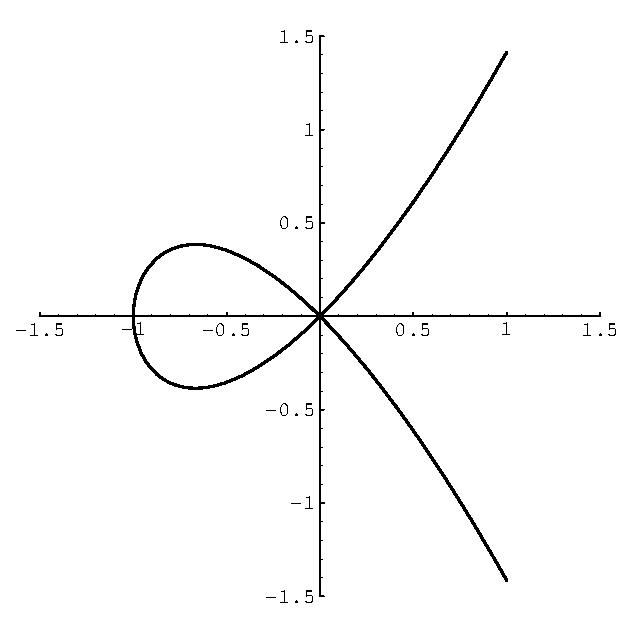
\includegraphics[width=2truein]{henselsg} &
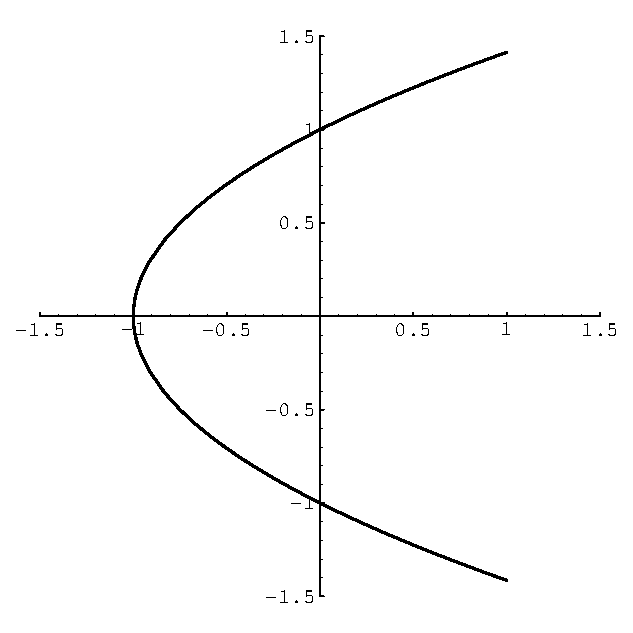
\includegraphics[width=2truein]{henselns} \\
(a) & (b)
\end{tabular}
\end{center}
\caption{The curves $Z^2 - t^3 -t^2$ and $Z^2 - t -1$
 \label{HenselSing:Fig}}
\end{figure}

As an example of what occurs when the derivative vanishes, consider
the polynomial
\[
F(Z) = Z^2 - t^2 - t^3,
\]
over the field $K = \Q(t)$.  If $F(Z)$ is square free and has two
distinct zeroes in $K_{(t)} = \Q((t))$:
\[
\begin{aligned}
\alpha & = t + \frac{t^2}{2} + \frac{t^3}{8} + \cdots, \\
\beta & =  - t - \frac{t^2}{2} - \frac{t^3}{8} - \cdots.
\end{aligned}
\]
However, modulo $\mathfrak{m} = (t)$ $F(Z)$ is not square free since the
constant terms of $\alpha$ and $\beta$ are the same.  

This situation is described geometrically in
\figref{HenselSing:Fig}(a).  In general, there are two points on the 
curve of $Z^2 - t^2 - t^3$ lying above any point on the horizontal,
$t$ axis.  At $t=0$ however, these two curve segments come together
at, what is called a \keyi{singular point} of the algebraic curve.

We can {\em desingularize} the curve at $t=0$, by focusing on the
second term in the power series expansion of $\alpha$ and $\beta$ not
the first.  That is, we replace $Z$ by $t Z'$.  This gives the new
equation:
\[
t^2 {Z'}^2 - t^2 -t^3 = 0.  
\]
So we can replace $F(Z)$ by $G(Z') = {Z'}^2 - 1 -t$.  This polynomial does
not have repeated roots modulo $\mathfrak{m}$ as is clear from
\figref{HenselSing:Fig}(b). 

More generally, assume that we have a polynomial $F(Z)$ over a ring
$R$ that is square free, but where $F(Z)$ is not square free over
$R/\mathfrak{p}$.  Further, assume that $\mathfrak{p} = (p)$ is a principal
ideal.  Since $F(Z)$ is not square free, it has more than one zero
lying over the point $\mathfrak{p}$ but which agree modulo $\mathfrak{p}$,
\eg,
\[
\begin{aligned}
\alpha & = a_0 + a_1 p + a_2 p^2 + a_3 p^3 + \cdots, \\
\beta  & = a_0 + b_1 p + b_2 p^2 + b_3 p^3 + \cdots.
\end{aligned}
\]
We can desingularize $F$ by using the new polynomial
\[
\frac{1}{p} F(p(Z - a_0))
\]
in place of $F(Z)$.  

The transformation described in the previous paragraph is called a
\keyi{blow up}.  It is known that blowup type transformations are
sufficient for desingularizing algebraic 
curves.\index{desingularization}  By repeatedly 
performing ``blow ups'' we can separate zeroes that agree modulo
$\mathfrak{p}^k$ for arbitrarily large, but finite $k$.  We can then
apply Newton's method to the desingularized equation to produce
approximations to the roots of arbitrary order.  

Note that if $F(Z)$ is not square free over $R$ then it is never
possible to separate the zeroes.

\section{Multidimensional Iteration}
\label{Multivariate:Newton:Sec}

Just as in the single variable case, the multivariate version of
Newton's iteration begins with \key{Taylor's formula}, this time in several
variables: Let $f(Z_1, \ldots, Z_n)$ be a polynomial in the variables
$Z_1, \ldots, Z_n$.  Its Taylor series expansion at $(x_1,\ldots,
x_n)$ is
\begin{equation}\label{Hensel:8}
\begin{aligned}
  \multispan{1}{$f(Z_1,\ldots, Z_n)$}\\
    \qquad = f(x_1,\ldots, x_n) &\null + 
    \sum_{i=1}^n {\partial f \over \partial Z_i}(x_1,\ldots,x_n) 
    (Z_i - x_i)\\
   & + {1 \over 2} \sum_{i=1}^n \sum_{j=1}^n
    {\partial^2 f \over \partial Z_i \, \partial Z_j}(x_1,\ldots,x_n) 
    (Z_i - x_i) (Z_j - x_j)\\
   & + \cdots\\
\end{aligned}
\end{equation}

The first summation in equation \eqnref{Hensel:8} is the inner product
of the row vector
\[
{\partial f \over \partial \vec{Z}} (\vec{x}) =
\left({\partial f \over \partial Z_1} (\vec{x}), 
{\partial f \over \partial Z_2} (\vec{x})
\ldots, {\partial f \over \partial Z_n} (\vec{x}) \right).
\]
and the column vector
\[
(\vec{Z} - \vec{x}) = \begin{pmatrix}Z_1 - x_1\\ \vdots\\ Z_n - x_n\end{pmatrix},
\]
where we have used $\vec{x}$ as an abbreviation for $(x_1, x_2, \ldots,
x_n)$ as in \sectref{Poly:Generalities:Sec}.  Using this notation, the
first two terms of \key{Taylor's formula} can be expressed as
\[
f(\vec{Z} ) = f(\vec{x}) + {\partial f \over \partial \vec{Z}}
(\vec{x}) \cdot (\vec{Z}  - \vec{x}) + \cdots.
\]

More generally, let $R$ be commutative ring, $\mathfrak{m}$ a maximal
ideal of $R$ and $\vec{f} = (f_1,\ldots,f_m)$ be a map from $R_\mathfrak{
m}^n$ to $R_\mathfrak{m}^m$.  It can be locally represented as a
multivariate power series expansion at $\vec{x}$
\[
\vec{f} (\vec{Z}) = \vec{f}(\vec{x}) 
  + \mathbf{J}(\vec{x})\cdot(\vec{Z} - \vec{x}) 
  + \cdots
\]
where $\mathbf{J}(\vec{x})$ is the \keyi{Jacobian} of the map $\vec{f}$:
\[
\mathbf{J}(\vec{x}) = 
\frac{\partial \vec{f}}{\partial \vec{Z}}
=
\begin{pmatrix}{\partial f_1\over \partial Z_1}& {\partial f_1\over \partial Z_2}&
 \cdots&{\partial f_1\over \partial Z_n}\\
{\partial f_2\over \partial Z_1}& {\partial f_2\over \partial Z_2}&
 \cdots&{\partial f_2\over \partial Z_n}\\
\vdots&\vdots&\ddots&\vdots\\
{\partial f_m\over \partial Z_1}& {\partial f_m\over \partial Z_2}&
 \cdots&{\partial f_m\over \partial Z_n}\end{pmatrix}.
\]
Again, letting $\vec{\alpha}$ be an element of the kernel of $\vec{f}$ and
expanding $\vec{f}$ at $\vec{\alpha} - \vec{\alpha}^{(k-1)}$, we have
\begin{equation}
0 = \vec{f}(\vec{\alpha}^{(k-1)}) + \mathbf{J}(\vec{\alpha}^{(k-1)}) 
\cdot (\vec{\alpha}  - \vec{\alpha}^{(k-1)}) +
O\left((\vec{\alpha} - \vec{\alpha}^{(k-1)})^{2}\right).
\label{MNewton:1:Eq}
\end{equation}

The term $O\left((\vec{\alpha} - \vec{\alpha}^{(k-1)})^{2}\right)$ is an
element of $\mathfrak{m}^{2}$.  If the rank of the Jacobian matrix is $n$
then the coordinates are well determined.  Choosing those rows of
\eqnref{MNewton:1:Eq} that are independent gives
\begin{equation}\label{MNewton:2:Eq}
\vec{\alpha}^{(2k-1)} - \vec{\alpha}^{(k-1)} 
  = -\mathbf{J}(\vec{\alpha}^{(k-1)})^{-1} 
  \cdot \vec{f}(\vec{\alpha}^{(k-1)}), \pmod{\mathfrak{m}^{2k}}
\end{equation}
which is quite similar to the quadratically convergent univariate iteration
\eqnref{Basic:UNewton:Eq}.  Equation \eqnref{MNewton:2:Eq} permits us to 
compute the element of 
$(R_\mathfrak{m})^n$ that lies over $\vec{\alpha_0}$.  However, this iteration
requires a matrix inversion at each step using a quadratically convergent 
iteration.  One way to eliminate the repeated matrix inversions is to use 
a linearly convergent version of \eqnref{MNewton:2:Eq}
\begin{equation}\label{MNewton:Lin:Eq}
\vec{\alpha}^{(k)} - \vec{\alpha}^{(k-1)}
   = -\mathbf{J}(\vec{\alpha}^{(0)})^{-1} 
  \cdot \vec{f}(\vec{\alpha}^{(k-1)}). \pmod{\mathfrak{m}^{k+1}}
\end{equation}

The linearly convergent iteration constructively shows that if the
Jacobian of a system of polynomial equations is invertible, a zero of
$\vec{f}(\vec{Z})$ modulo $\mathfrak{m}$ can always be lifted to a zero
modulo $\mathfrak{m}^k$ for any $k$.  That is,

\begin{proposition}\label{MNewton:Iter:Prop}
Assume $R$ is an integral domain with an ideal $\mathfrak{m}$.  Let
$\vec{f} = (f_1(Z_1, \ldots, Z_n), \ldots, f_n(Z_1, \ldots, Z_n))$ be
polynomials over $R$ and denote their Jacobian with respect to the
$Z_i$ by $\mathbf{J}$.  Let $(x_1, \ldots, x_n)$ be a zero of $\vec{f}$
modulo $\mathfrak{m}$ such that the determinant of $\mathbf{J}(x_1, \ldots,
x_n)$ has an inverse in $R/\mathfrak{m}$.  Then there exist unique
elements $\hat{x}_1, \ldots, \hat{x}_n$ of $R_\mathfrak{m}$, $\hat{x}_i =
x_i \mod\mathfrak{m}$, for which $\vec{f}(\hat{x}_1, \ldots, \hat{x}_n)
= 0$.
\end{proposition}

\begin{proof}
Let $\alpha_i^{(0)} = x_i$.  Since $\mathbf{J}(x_1, \ldots, x_n)$ is
invertible modulo $\mathfrak{m}$ we can repeatedly apply
\eqnref{MNewton:Lin:Eq} to compute $\vec{\alpha}^{(k)}$ for any
$k$.  The $\vec{\alpha}_i^{(k)}$ form a \key{coherent sequence} whose
limit is $\hat{x}_i$.

Thus there exists a point $(\hat{x}_1, \ldots, \hat{x}_n)$ that
satisfies the conditions of the proposition.  Assume that $(\hat{y}_1, 
\ldots, \hat{y}_n)$ also satisfies the proposition and that $k$ is the 
smallest value for which 
\begin{equation} \label{MNewton:NotEq:Eq}
\hat{x}_i \not= \hat{y}_i \pmod{\mathfrak{m}^{k+1}}
\end{equation}
for some $i$. Note that $k$ must be positive. We can denote by
$\vec{\alpha}^{(k-1)}$:
\[
(\hat{x}_1, \ldots, \hat{x}_n) = (\hat{y}_1, \ldots, \hat{y}_n) =
\vec{\alpha}^{(k-1)} \pmod{\mathfrak{m}^k}
\]
But then we have:
\[
\begin{aligned}
(\hat{x}_1, \ldots, \hat{x}_n) - \vec{\alpha}^{(k-1)}
   &= -\mathbf{J}(\vec{\alpha}^{(0)})^{-1} 
  \cdot \vec{f}(\vec{\alpha}^{(k-1)}), \\
(\hat{y}_1, \ldots, \hat{y}_n) - \vec{\alpha}^{(k-1)}
   &= -\mathbf{J}(\vec{\alpha}^{(0)})^{-1} 
  \cdot \vec{f}(\vec{\alpha}^{(k-1)}),
\end{aligned}
\pmod{\mathfrak{m}^{k+1}}
\]
which contradicts \eqnref{MNewton:NotEq:Eq}.
\end{proof}

\paragraph{Quadratic Iteration}

The need to repeatedly invert the Jacobian of the system can also be 
eliminated by applying Newton's method to the equation for the reciprocal 
of the Jacobian as described was done in
\sectref{Univariate:Newton:Sec}.\Marginpar{Rewrite this paragraph}
We apply \eqnref{MNewton:2:Eq} to the system linear of equations
\[
\mathbf{X} \cdot \mathbf{J}(\alpha) = {\bf 1}
\]
where both $\bf X$ and $\bf 1$ are $n\times n$ matrices, and the
components of $\bf X$ are to be determined.  Given
$\mathbf{\Upsilon}^{(k-1)}$ such that 
\[
\mathbf{\Upsilon}^{(k-1)} \cdot \mathbf{J}(\vec{\alpha}) = 
\mathbf{\Upsilon}^{(k-1)} \cdot \mathbf{J}(\vec{\alpha}^{(2k-1)}) = {\bf 1},
  \pmod{\mathfrak{m}^{k}}
\]
we want to find $\mathbf{\Upsilon}^{(2k-1)}$ where
\begin{equation} \label{Jacobian:1:Eq}
\mathbf{\Upsilon}^{(2k-1)} \cdot \mathbf{J}(\alpha^{(2k-1)}) = {\bf 1} \pmod{\mathfrak{m}^{2k}}
\end{equation}
We interpret the matrix equation \eqnref{Jacobian:1:Eq} as system of 
$n^{2}$ linear equations in $n^{2}$ unknowns, where the unknowns are the 
entries of $\mathbf{\Upsilon}^{(2k-1)}$. 

The Jacobian of \eqnref{Jacobian:1:Eq} is a block diagonal
$n^{2}\times n^{2}$ matrix, where each block contains
$\mathbf{J}(\alpha^{(2k-1)})^{T}$.  Since we only need to compute the
inverse of this matrix modulo $\mathfrak{m}^{k}$, we can write its
inverse as
\[
\begin{aligned}
\begin{pmatrix}
 \mathbf{J}(\alpha^{(2k-1)})^T & {\bf 0} & \cdots & {\bf 0}\\
 {\bf 0} & \mathbf{J}(\alpha^{(2k-1)})^T & \cdots & {\bf 0} \\
 \vdots  & & & \vdots \\
 {\bf 0} & {\bf 0} & \cdots & \mathbf{J}(\alpha^{(2k-1)})^T \end{pmatrix}^{-1} \qquad\\
 = 
\begin{pmatrix}
 \mathbf{\Upsilon}^{(k-1) \, T} & {\bf 0} & \cdots & {\bf 0}\\
 {\bf 0} & \mathbf{\Upsilon}^{(k-1) \, T} & \cdots & {\bf 0} \\
 \vdots  & & & \vdots \\
 {\bf 0} & {\bf 0} & \cdots & \mathbf{\Upsilon}^{(k-1) \, T} \end{pmatrix}
\end{aligned}
\pmod{\mathfrak{m}^{k}}
\]
According to \eqnref{MNewton:2:Eq}, $\vec{\mathbf{J}}^{(2k-1)} - \vec{\mathbf{J}}^{(k)}$
is equal to the product of this matrix multiplied on the right by the
vector of entries of 
\[
\mathbf{\Upsilon}^{(k-1)} \cdot \mathbf{J}(\alpha^{(2k-1)}) - {\bf 1} \pmod{\mathfrak{m}^{2k}}.
\]
Due to the repetitive structure of the Jacobian, we can write this as 
\begin{equation}
\mathbf{\Upsilon}^{(2k-1)} - \mathbf{\Upsilon}^{(k-1)} =
({\bf 1} - \mathbf{\Upsilon}^{(k-1)} \cdot \mathbf{J}(\vec{\alpha}^{(2k-1)})) \cdot 
\mathbf{\Upsilon}^{(k-1)} \pmod{\mathfrak{m}^{2k}}
\label{MNewton:3:Eq}
\end{equation}

Putting this together with \eqnref{MNewton:2:Eq} we have
\begin{equation}
\label{Quasi:MNewton:Eq}
 \begin{aligned}
   \vec{\alpha}^{(2k-1)} - \vec{\alpha}^{(k-1)} & 
      = -\mathbf{\Upsilon}^{(k-1)}\cdot \vec{f}(\vec{\alpha}^{(k-1)}) \\
   \mathbf{\Upsilon}^{(2k-1)} - \mathbf{\Upsilon}^{(k-1)} &=
     ({\bf 1} - \mathbf{\Upsilon}^{(k-1)} \cdot \mathbf{J}(\vec{\alpha}^{(2k-1)})) 
          \cdot \mathbf{\Upsilon}^{(k-1)}
 \end{aligned}
 \pmod{\mathfrak{m}^{2k}}
\end{equation}
which is the basic quadratically convergent multivariate iteration.

To illustrate the steps leading from \eqnref{Jacobian:1:Eq} to
\eqnref{MNewton:3:Eq}, we consider the $2 \times 2$ case explicitly:
\[
\begin{aligned}
\mathbf{X}^{(2k-1)} \cdot \mathbf{M}^{(2k-1)} 
& = 
\begin{pmatrix}x_{11}^{(2k-1)} & x_{12}^{(2k-1)} \\\noalign{\vskip3pt}
x_{21}^{(2k-1)} & x_{22}^{(2k-1)} \end{pmatrix} 
\cdot
\begin{pmatrix}m_{11}^{(2k-1)} & m_{12}^{(2k-1)} \\\noalign{\vskip3pt}
m_{21}^{(2k-1)} & m_{22}^{(2k-1)} \end{pmatrix} \\
& = \begin{pmatrix}1& 0 \\ 0 & 1 \end{pmatrix},
\end{aligned}
\pmod{\mathfrak{m}^{2k}}
\]
where $\mathbf{M}^{(2k-1)}$ is the image modulo $\mathfrak{m}^{2k}$ of a
known matrix $\mathbf{M}$ and $\mathbf{X}^{(2k-1)}$ is a matrix whose elements
are to be determined.  The correspondence to our case is
$\mathbf{X}^{(2k-1)} = \mathbf{\Upsilon}^{(2k-1)}$ and $\mathbf{M}^{(2k-1)} =
\mathbf{J}(\vec{\alpha}^{(2k-1)})$. In terms of their components, these
equations are 
\[
\begin{aligned}
 f_1(x_{11}, x_{12}, x_{21}, x_{22}) & 
   = m_{11} x_{11} + m_{21} x_{12} - 1, \\
 f_2(x_{11}, x_{12}, x_{21}, x_{22}) & 
   = m_{12} x_{11} + m_{22} x_{12}, \\ 
 f_3(x_{11}, x_{12}, x_{21}, x_{22}) & 
   = m_{11} x_{21} + m_{21} x_{22}, \\ 
 f_4(x_{11}, x_{12}, x_{21}, x_{22}) & 
   = m_{12} x_{21} + m_{22} x_{22} - 1,
\end{aligned}
\]
which gives a Jacobian of 
\[
\begin{pmatrix}
   m_{11} & m_{21} & 0 & 0 \\
   m_{12} & m_{22} & 0 & 0 \\
   0 & 0 & m_{11} & m_{21} \\
   0 & 0 & m_{12} & m_{22} \end{pmatrix}.
\]
Using \eqnref{MNewton:2:Eq}, the quadratic iteration for the solution
of this system of equations is
\[
\begin{aligned}
\null & \begin{pmatrix}
  x_{11}^{(2k-1)} - x_{11}^{(k-1)} \\
  x_{12}^{(2k-1)} - x_{12}^{(k-1)} \\
  x_{21}^{(2k-1)} - x_{21}^{(k-1)} \\
  x_{22}^{(2k-1)} - x_{22}^{(k-1)} \end{pmatrix} \\
\null & \qquad =
- \begin{pmatrix}
   j_{11}^{(k-1)} & j_{21}^{(k-1)} & 0 & 0 \\
   j_{12}^{(k-1)} & j_{22}^{(k-1)} & 0 & 0 \\
   0 & 0 & j_{11}^{(k-1)} & j_{21}^{(k-1)} \\
   0 & 0 & j_{12}^{(k-1)} & j_{22}^{(k-1)} \end{pmatrix}
\cdot
\begin{pmatrix}
  f_1(\vec{x}^{(k-1)}) \\ 
  f_2(\vec{x}^{(k-1)}) \\
  f_3(\vec{x}^{(k-1)}) \\ 
  f_4(\vec{x}^{(k-1)}) \end{pmatrix} \\
\null & \qquad = - \begin{pmatrix}
    j_{11}^{(k-1)}f_1(\vec{x}^{(k-1)}) + j_{21}^{(k-1)}f_2(\vec{x}^{(k-1)})\\
    j_{12}^{(k-1)}f_1(\vec{x}^{(k-1)}) + j_{22}^{(k-1)}f_2(\vec{x}^{(k-1)})\\
    j_{11}^{(k-1)}f_3(\vec{x}^{(k-1)}) + j_{21}^{(k-1)}f_4(\vec{x}^{(k-1)})\\
    j_{12}^{(k-1)}f_3(\vec{x}^{(k-1)}) + j_{22}^{(k-1)}f_4(\vec{x}^{(k-1)})
    \end{pmatrix}
\\
\end{aligned}
\pmod{\mathfrak{m}^{2k}}
\]
This can be rewritten as a product of $2 \times 2$ matrices as 
\[
\begin{aligned}
\null & \begin{pmatrix}
  x_{11}^{(2k-1)} - x_{11}^{(k-1)} &
  x_{12}^{(2k-1)} - x_{12}^{(k-1)} \\
  x_{21}^{(2k-1)} - x_{21}^{(k-1)} &
  x_{22}^{(2k-1)} - x_{22}^{(k-1)} \end{pmatrix} \\
\null & \qquad =
\begin{pmatrix}
  f_1(\vec{x}^{(k-1)}) & f_2(\vec{x}^{(k-1)}) \\
  f_3(\vec{x}^{(k-1)}) & f_4(\vec{x}^{(k-1)}) \end{pmatrix}
\cdot
\begin{pmatrix}
   j_{11}^{(k-1)} & j_{12}^{(k-1)} \\
   j_{21}^{(k-1)} & j_{22}^{(k-1)} \end{pmatrix}
\end{aligned}
\]


The initial solution of the system of equations, $\vec{\alpha}_{0}$ is
called the starting point of the iteration.  If
$\mathbf{J}(\vec{\alpha}_0)$ is invertible then $\vec{\alpha}_0$ is said
to be a \keyi{good starting point}.  If the Jacobian matrix is not
invertible, either because the $\vec{\alpha}_0$ was a bad starting
point or because the Jacobian itself was not square, then the system
of linear equations that need to be solved at each step will not have a
unique solution.  There are cases where this can be useful, for
instance as a sieve for possible solutions to diophantine 
equations\index{diophantine equation}
over the integers.

\section{Hensel's Lemma}
\label{Hensel:Lemma:Sec}
\index{Hensel's lemma|(}

One of the the most useful theorems in commutative algebra is {\em
Hensel's lemma}.  Essentially, it says that if a monic polynomial with
coefficients in a ring $R$ factors modulo an ideal $\mathfrak{m}$, then
it factors as a polynomial over $R_\mathfrak{m}$.  More precisely,

\begin{proposition}[Hensel's Lemma] \label{Hensel:Lemma:Prop}
Let $F(Z)$ be a monic polynomial over an integral domain $R$,
$\mathfrak{m}$ an ideal of $R$.  If there exist polynomials $G(Z)$ and
$H(Z)$ over $R/\mathfrak{m}$ such that 
\[
F(Z) = G(Z) H(Z) \pmod\mathfrak{m}
\]
and $G(Z)$ and $H(Z)$ are relatively prime as polynomials over
$R/\mathfrak{m}$, then there exist polynomials $\hat{G}(Z)$ and
$\hat{H}(Z)$ over $R_\mathfrak{m}$ such that
\[
\begin{aligned}
G(Z) & = \hat{G}(Z) \\ H(Z) & = \hat{H}(Z)
\end{aligned}
\pmod\mathfrak{m}
\]
and $F(Z) = \hat{G}(Z) \hat{H}(Z)$ over $R_\mathfrak{m}$.
\end{proposition}

Although, this proposition is phrased in terms of polynomials in $R[Z]$, 
the variable $Z$ is only used as a place holder that allows us to 
succinctly describe a system of non-linear equations.  This is clarified 
in the following proof. 

\begin{proof}
Let the degree of $F$ in $Z$ be $d$ and that of $G(Z)$ and $H(Z)$ be
$r$ and $s$ respectively, $r+s = d$.  We denote the coefficients of
$F$ by $f_i$,
\[
F(Z) = Z^d + f_1 Z^{d-1} + \cdots + f_d,
\]
where $f_i \in R$.  And the coefficients of $G$ and $H$ by $g^{(0)}_i$
and $h^{(0)}_i$:
\[
\begin{aligned}
G(Z) &= Z^r + g^{(0)}_1 Z^{r-1} + \cdots + g^{(0)}_r, \\
H(Z) &= Z^s + h^{(0)}_1 Z^{s-1} + \cdots + h^{(0)}_s,
\end{aligned}
\]
where $g^{(0)}_i$ and $h^{(0)}_i$ are elements of $R/\mathfrak{m}$.

If $G$ and $H$ can be lifted to polynomials over
$R_\mathfrak{m}$, then we can write
\[
\begin{aligned}
\hat{G}(Z) & = Z^r + g_1 Z^{r-1} + \cdots + g_r, \\
\hat{H}(Z) & = Z^s + h_1 Z^{s-1} + \cdots + h_s, 
\end{aligned}
\]
where $g_i$ and $h_i$ are unknown elements of $R_\mathfrak{m}$.
Expanding $\hat{G}(Z) \hat{H}(Z) = F(Z)$ and equating coefficients of
$Z$ we have
\begin{equation}\label{Hensel:Eq}
\begin{aligned}
  g_1 + h_1&= f_1,\\
  g_2 + g_1h_1 + h_2&= f_2,\\
  \vdots&\\
  g_r h_{s-1} + g_{r-1} h_s&= f_{n-1},\\
  g_r h_s&= f_n.
\end{aligned}
\end{equation}
This is a system of $d$ equations if $r+s$ unknowns and is called the
\keyi{coefficient equations} of the factorization $F = \hat{G}\cdot
\hat{H}$.  Any factorization of $F(Z)$ into factors of degree $r$ and
$s$ leads to a solution of \eqnref{Hensel:Eq}.  Conversely, any
solution of \eqnref{Hensel:Eq} leads to a factorization of $F(Z)$.
Thus solving \eqnref{Hensel:Eq} and factoring $F(Z)$ are equivalent. 

The coefficients of $G(Z)$ and $H(Z)$ are a solution of
\eqnref{Hensel:Eq} modulo $\mathfrak{m}$.  By \propref{MNewton:Iter:Prop} this
solution can be uniquely lifted to a solution in $R_\mathfrak{m}$ if the
Jacobian of \eqnref{Hensel:Eq} is non-singular.

The Jacobian of \eqnref{Hensel:Eq} can be computed directly:
\[
\left(
\begin{array}{cccccccc}
  1 &   0 & \ldots &   0 &   1 &   0 & \ldots & 0 \\
h_1 &   1 &        &   0 & g_1 &   1 &        & 0 \\
h_2 & h_1 & \ldots &   0 & g_2 & g_1 & \ldots & 0 \\
\vdots&   &        &     & \vdots&   &        &\vdots\\
0   &   0 & \ldots & h_s & 0   &   0 & \ldots &g_r
\end{array}
\right),
\]
the \key{Sylvester matrix} for the \key{resultant} of $G(Z)$ and
$H(Z)$, as was pointed out in \sectref{Poly:Resultant:Sec}.  It is
known to be zero if and only if $g$ and $h$ have a nontrivial common
factor.  Since $G(Z)$ and $H(Z)$ are assumed to be relatively prime,
the Jacobian is always non-singular.
\end{proof}

\paragraph{Example}

Consider the polynomial 
\[
F(Z) = Z^5 +Z^4 + 2Z^2 + 2Z + 3.
\]
Modulo $5$ it can be factored
\begin{equation}\label{Hensel:Ex5:Eq}
F(Z) = (Z^3 + 4Z + 3) (Z^2 + Z + 1) \pmod{5}
\end{equation}
Suspecting that $F(Z)$ factors into a quadratic and a cubic factor
over the rational integers we use \longpropref{Factor:CBound:Prop} to
bound the size of the coefficients of its factors.  If $G$ and $H$ are
the cubic and quadratic factors of $F$ over the integers, then
\[
(d+1)^{1/2} 2^d |F| = \sqrt{6}\, 2^5\times 3 \approx 8465 \ge \max \{
|G|, |H|\}.
\]
So we should lift the factorization of $F(Z)$ to one modulo $5^7 > 2
\times 9000$.

The \keyi{coefficient equations} corresponding to the factorization of
$F(Z)$ into a cubic and quadratic factor are
\begin{equation} \label{MNewton:Sing:Eq}
\begin{aligned}
a_1 + b_1 & = 1, \\
a_2 + a_1 b_1 + b_2 & = 0, \\
a_3 + a_2 b_1 + a_1 b_2 & = 2, \\
a_3 b_1 + a_2 b_2 & = 2, \\
a_3 b_2 & = 3.
\end{aligned}
\end{equation}
The Jacobian of this system of equations is 
\[
\left(
\begin{array}{ccccc}
1 & 0 & 0 & 1 & 0 \\
b_1 & 1 & 0 & a_1 & 1 \\
b_2 & b_1 & 1 & a_2 & a_1 \\
0   & b_2 & b_1 & a_3 & a_2 \\
0   & 0   & b_2 & 0   & a_3
\end{array}
\right).
\]
We can verify that this matrix is non-singular when the $a_i$ and
$b_i$ are replaced by their corresponding values from
\eqnref{Hensel:Ex5:Eq}.  By applying the multivariate version of Newton's
iteration \eqnref{MNewton:Lin:Eq} we get 
\[
\begin{aligned}
a_1 & = 0 + 0\cdot 5 + 0 \cdot 5^2 + 0 \cdot 5^3 + \cdots, \\
a_2 & = 6 + 6\cdot 5 + 6 \cdot 5^2 + 6 \cdot 5^3 + \cdots, \\
a_3 & = 3 + 0\cdot 5 + 0 \cdot 5^2 + 0 \cdot 5^3 + \cdots, \\
b_1 & = 1 + 0\cdot 5 + 0 \cdot 5^2 + 0 \cdot 5^3 + \cdots, \\
b_2 & = 1 + 0\cdot 5 + 0 \cdot 5^2 + 0 \cdot 5^3 + \cdots. \\
\end{aligned}
\]

Modulo $7$ however we get the factorization
\[
f(Z) = (Z^3 + 6 Z + 3) (Z^2 +  Z + 1).
\]
These factors are not irreducible and share a common factor of
$X+3$.  The Jacobian in this case is 
\[
\left(
\begin{array}{ccccc}
1 & 0 & 0 & 1 & 0 \\
1 & 1 & 0 & 0 & 1 \\
1 & 1 & 1 & 6 & 0 \\
0 & 1 & 1 & 3 & 6 \\
0 & 0 & 1 & 0 & 3
\end{array}
\right),
\]
whose integer determinant is $4 \times 7$.

\label{PolyZ7:SQFR:Ex}
Although $F(Z)$ is not square free over $\Z/(7)$ it does have three
distinct zeroes in $\Z_7$:
\[
\begin{aligned}
\alpha_1 & = 4 + 2\cdot 7 + 0\cdot 7^2 + 3\cdot 7^3 + 6\cdot 7^4 +
4\cdot 7^5 + 0\cdot 7^6 + 4\cdot 7^7 + \cdots \\
\alpha_2 & = 4 + 1\cdot7 + 3\cdot7^2 + 6\cdot7^3 + 0\cdot7^4 + 2\cdot7^5
+ 5\cdot7^6 + 1\cdot7^7 + \cdots \\
\alpha_3 & = 2 + 4\cdot7 + 6\cdot7^2 + 3\cdot7^3 + 0\cdot7^4 +
2\cdot7^5 + 6\cdot7^6 + 2\cdot7^7 + \cdots
\end{aligned}
\]
This explains the indeterminacy of the factorization.  The quadratic
factor could be either
\[
(Z - \alpha_1) \cdot (Z - \alpha_3) \quad\mbox{or}\quad
(Z - \alpha_2) \cdot (Z - \alpha_3).
\]
Both factorizations have the same image modulo $7$.  Since $7^2$ does
not divide the determinant of the Jacobian, these two factorizations
can be differentiated by their images modulo $7^2$.

The system of equations \eqnref{MNewton:Sing:Eq} describes an
algebraic surface embedded in a five dimensional space.  The fact that
the Jacobian is divisible by $7$ means that the surface has a singular
point at $(7)$.  It is possible to desingularize surface by blow ups
as described in the unvariate case,\index{desingularization} \index{blow 
up} but the discussion would take us too far a field.

\index{Hensel's lemma|)}

\section{Generalizations of Hensel's Lemma}
\label{General:Hensel:Sec}

While Hensel's lemma is usually expressed in terms of factoring a
polynomial into two relatively prime factors, the technique given in
the previous section can be applied more generally. 

Consider what happens if $F(Z)$ has three factors modulo
$\mathfrak{m}$, \ie, $F(Z) = A(Z) \cdot B(Z) \cdot C(Z)$ modulo
$\mathfrak{m}$ and $A(Z)$, $B(Z)$, and $C(Z)$ have degrees $r_1$,
$r_2$ and $r_3$ respectively, $r = r_1 + r_2 + r_3$.  We then know
that
\[
\begin{aligned}
  Z^r + \cdots + f_r&=
    (Z^{r_1} + \cdots + a_{r_{1}}) (Z^{r_2} + \cdots + b_{r_{2}})
    (Z^{r_3} + \cdots + c_{r_{3}}),\\
   &= Z^{r_1 + r_2 + r_3} + (a_{1} + b_{1} + c_{1}) Z^{r_1 + r_2 + r_3 -1} 
    + \cdots + a_{r_{1}} b_{r_{2}} c_{r_{3}}.
\end{aligned}
\]
If we equate the coefficients $Z^i$ on the right hand side of the
equation with those on the left hand side, we get a system of $r = r_1 + 
r_2 + r_3$ algebraic equations in $r$ unknowns.  The Jacobian of this 
system is a $r\times r$ matrix, $\mathbf{J}_1$ whose first $r_1$ columns 
look like 
\[
\overbrace{
\begin{array}{cccc}
1 & 0 & \cdots  & 0 \\
b_1 + c_1 & 1 & \cdots & 0\\
b_2 + b_1 c_1 + c_2 & b_1 + c_1 &  \cdots & 0 \\
\vdots & & & \vdots \\
0 & 0 & \cdots & b_{r_2} c_{r_3} \\
\end{array}}^{r_1}
\]
The next $r_2$ and $r_3$ columns are organized similarly.  By
\propref{MNewton:Iter:Prop}, when $\mathbf{J}_1$ is invertible over
$R/\mathfrak{m}$ the factorization $F = A \cdot B \cdot C$ can be lifted
{\em uniquely} to a factorization of $F$ in $R_\mathfrak{m}$.  When there
are just two factors, non-singularity of the Jacobian corresponds to
the factors being relatively prime.  What criteria corresponds to the
invertibility of $\mathbf{J}_1$?

If $A(Z)$ and $B(Z)$ are not relatively prime modulo $\mathfrak{m}$, then
the lift is certainly not unique, and similarly for the other pairings.
Thus, we expect that
\[
R = (\res_Z (A(Z), B(Z))) \cdot (\res_Z (A(Z), C(Z))) 
  \cdot (\res_Z (B(Z), C(Z)))
\]
divides the determinant of $\mathbf{J}_1$.  The term with maximum total 
degree in $R$ has total degree 
\[
(r_1 + r_2 - 1) + (r_1 + r_3 - 1) + (r_2 + r_3 - 1) = 2r -3.
\]
Examining the degrees of the rows of $\mathbf{J}_1$ we see that the monomial
of maximum total degree in 
the determinant of $\mathbf{J}_1$ has total degree
\[
0 + 1 + \overbrace{2 + 2 + \cdots + 2}^{r-2} = 2r -3.
\]
Thus,
\[
\det \mathbf{J}_1 = (\res_Z (A(Z), B(Z))) \cdot (\res_Z (A(Z), C(Z))) 
  \cdot (\res_Z (B(Z), C(Z))).
\]
Similar reasoning extends this result to an arbitrary number of
pairwise relatively prime factors.  

\smallskip
More generally, assume we have a monic polynomial $F(Z)$ over a ring
$R$ that has a factorization
\begin{equation} \label{Hensel:NSQ:Eq}
F(Z) = P_1^{e_1}(Z) \cdot P_2^{e_2}(Z) \cdots P_n^{e_n}(Z)
\pmod{\mathfrak{m}}
\end{equation}
The previous paragraphs discussed the case when the $e_i$ are equal to
$1$.  The coefficient equations of this factorization can be formed in
the same way as in the previous discussion.  Now, however, the number
equations exceeds the number unknowns.  Since there is a one to one
correspondence between factorizations $F(Z)$ of the form
\eqnref{Hensel:NSQ:Eq} and zeroes of the system of coefficient
equations, the coefficient equations must be consistent.

An interesting illustration of this approach is to lift the
factorization 
\[
\begin{aligned}
F(Z) & = Z^5 + Z^4 + 2Z^2 + 2Z + 3, \\
  & = (Z+3)^2 (Z+5) (Z^2 + 4Z+1),
\end{aligned}
\pmod{7}
\]
to a factorization over $\Z_7$.  On page \pageref{PolyZ7:SQFR:Ex} we showed that as
a polynomial over $\Z_7$ $F(Z)$ was square free.  Thus, this
factorization cannot be lifted to a factorization over $\Z_7$. Here we
show how the lifting process breaks down. possible since earlier $F(Z)$ was shown to be square free over $\Z_7$.

Assuming that
\begin{equation} \label{Hensel:NSQEx:Eq}
F(Z) =  (Z + a)^2  (Z+b) (Z^2+c_1Z+c_2)
\end{equation}
The coefficient equations are 
\[
\begin{aligned}
2a + b + c_1 & = 1, \\
a^2 + 2ab + 2 ac_1 + b c_1 + c_2 & = 0, \\
a^2 b + a^2 c_1 + 2 a b c_1 + 2 a c_2 + b c_2 & = 2, \\
a^2 b c_1 + a^2 c_2 + 2 a b c_2 & = 2, \\
a^2 b c_2 & = 3.
\end{aligned}
\]
The Jacobian of the first four equations, at $(a,b,c_1,c_2) =
(3,5,4,1)$ has integer determinant $48$.  Its inverse modulo $7$ is
\[
\left(
\begin{array}{cccc}
3 & 1 & 6 & 6 \\
4 & 0 & 3 & 4 \\
5 & 5 & 6 & 5 \\
1 & 6 & 5 & 6 
\end{array}
\right).
\]
Thus, we can uniquely lift the zero to a zero of the first four
equations in $\Z_7$:
\[
\begin{aligned}
a   & = 3 +         7 + 0 \cdot 7^2 + 6 \cdot 7^3 + 5 \cdot 7^4 + \cdots, \\
b   & = 5 + 2 \cdot 7 + 2 \cdot 7^2 + 1 \cdot 7^3 + 4 \cdot 7^4 + \cdots, \\
c_1 & = 3 + 1 \cdot 7 + 4 \cdot 7^2 + 0 \cdot 7^3 + 5 \cdot 7^4 + \cdots, \\
c_2 & = 1 + 3 \cdot 7 + 1 \cdot 7^2 + 1 \cdot 7^3 + 0 \cdot 7^4 +
\cdots.
\end{aligned}
\]
Unfortunately, this solution is not a zero of the final equation.
There the coefficient equations do not have a solution in $\Z_7$, just
as the polynomial $F(Z)$ does not have a factorization of the form
\eqnref{Hensel:NSQEx:Eq}.

\medskip
The {\sc gcd} problem can be handled in a similar manner.  Assume
we want to compute $H(Z)$, which is the {\sc gcd} of $F(Z)$ and $G(Z)$,
where $\deg F = r$, $\deg G = s$ and $\deg H = n$.  Letting $F(Z) =
A(Z) H(Z)$ and $G(Z) = B(Z) H(Z)$ we get the following system of
equations:
\[
\begin{aligned}
  a_1 + h_1 &= f_1\\
  a_2 + a_1 h_1 + h_2 &= f_2 \\
  \vdots\\
  a_{r - n} h_n & = f_r
\end{aligned} \qquad
\begin{aligned}
  b_1 + h_1 &= g_1\\
  b_2 + a_1 h_1 + h_2 &= g_2 \\
  \vdots\\
  b_{s - n} h_n & = g_r
\end{aligned}
\]
We now have $r+s$ equations, but only have $n + r -n + s - n = r + s
-n$ unknowns.  Thus, some of these equations are redundant if $F$
and $G$ actually have a unique {\sc gcd} of degree $n$.  Notice that
applying the Hensel approach to the {\sc gcd} problem gives a method
that lifts, not only $H$, but also the cofactors of $F$ and 
$G$.\index{cofactor} 

\section{Zassenhaus' Formulation of Hensel's Lemma}
\label{Zassenhaus:Formulation:Sec}

{\Zassenhaus}' version of \key{Hensel's lemma} differs from the one
discussed in the preceding sections in that the number of equations
produced is smaller than the number of variables.  For instance, in
the factoring problem, the Zassenhaus approach determines $G$ and $H$
by solving the equation
\begin{equation}
 \label{Zassen:Factor:Eq}
F(X) - G(X) \cdot H(X) = 0
\end{equation}
It is only when the solution of this equation is restricted to the ring
$\Z_{p}[X]$ that \eqnref{Zassen:Factor:Eq} has a unique solution.  By using
a $p$-adic technique the non-linear diophantine equation
\eqnref{Zassen:Factor:Eq} can be reduced to a series of easy to solve,
linear equations.  Then by piecing together the solutions of these linear
equations, $G$ and $H$ can be determined.  Here we outline the main 
points and demonstrate the connection with our formalism.

Let $F(X)$ be a univariate polynomial over the integers, and assume
that it has two irreducible factors, $G$ and $H$.  We are given a
factorization $F(X) = G_0 H_0$ modulo $p$ and we want to lift $G_0$
and $H_0$ to $G$ and $H$.  Writing $G$ and $H$ $p$-adically gives
\[
\begin{aligned}
  F(X) &= (G_0 + G_1 p + \cdots) (H_0 + H_1 p + \cdots), \\
   &= G_0 H_0 + (H_1 G_0 + G_1 H_0) p + \cdots.
\end{aligned}
\]
Modulo $p^2$ we have
\[
F(X) - G_0 H_0 = (H_1 G_0 + G_1 H_0) p \pmod{p^2}
\]
Since $F(X) - G_0 H_0$ is a multiple of $p$, dividing by $p$ gives 
\begin{equation}
H_1 G_0 + G_1 H_0 = \left( F(X) - G_0 H_0 \right) / p \qquad\pmod{p}
\label{Linear:Dio:Eq}
\end{equation}
This is a polynomial valued linear diophantine equation\index{diophantine 
equation!linear} in $G_1$ and $H_1$.  Its solution can be obtained by 
first solving $A_i G_0 + B_i H_0 = X^i \pmod{p}$ for various $i$ by the 
Euclidean algorithm.  Since the left hand side of \eqnref{Linear:Dio:Eq} 
is a polynomial in $X$, $G_1$ and $H_1$ can be determined by adding 
combinations of the appropriate $B_i$ and $A_i$ respectively.

Having computed $G_1$ and $H_1$, the other terms may be computed
similarly.  For a linear iteration, the process continues as follows:
\[
F(X) = (G_0 + G_1 p + G_2 p^2 + \cdots) 
(H_0 + H_1 p + H_2 p^2 + \cdots)
\]
Considering this equation modulo $p^3$
\[
(H_2 G_0 + G_2 H_0) = \left( F(Z) - 
  (G_0 + G_1 p)(H_0 + H_1 p) \right) / p^2 \qquad \pmod{p}
\]
The right hand side of this equation is again a polynomial and the
left hand side is essentially the same as \eqnref{Linear:Dio:Eq}.  So
using the $A_i$ and $B_i$ obtained in the previous step we can compute
$G_2$ and $H_2$.

\paragraph{Relation to Solving Equations}

The {\Zassenhaus} version of \key{Hensel's lemma} produces the same 
answer as the approach based on Newton's method discussed earlier---the 
correct factorization through each of the lifting stages.  The
following paragraphs demonstrate that this is not a fortuitous
accident but is due to the fact that both formulations are performing
the same computation in a slightly different manner.

The key to using {\Zassenhaus}'s formulation of \key{Hensel's lemma} to 
lift a factorization $F = G_0 H_0 \mod{\mathfrak{m}}$ to the $\mathfrak{
m}$-adic completion is solving the diophantine equations
\begin{equation} \label{Hensel:ZassDio:Eq}
A_i G_0 + B_i H_0 = Z^i \qquad\pmod{\mathfrak{m}}
\end{equation}
Once we have obtained the $A_i$ and $B_i$, it is merely a matter of
computing the error introduced when a factorization modulo $\mathfrak{m}^k$ 
is lifted to one modulo $\mathfrak{m}^{k+1}$.
This error is then used to produce the appropriate linear combination of the
$A_i$ and $B_i$ that is $G_{k+1}$ and  $H_{k+1}$.

Our formulation is quite similar.  We begin by inverting the Jacobian
matrix.  Through the Newton-Raphson formula we combine the error terms
to compute $G_{k+1}$ and $H_{k+1}$.  Structurally, these two algorithms 
are quite similar.  We shall see that the solutions of 
\eqnref{Hensel:ZassDio:Eq} form the inverse of the Jacobian matrix.

To see this let,
\[
\begin{aligned}
  G_0 &= Z^r + g_1 Z^{r-1} + g_2 Z^{r-2} + \cdots + g_r\\
  H_0 &=Z^s + h_1 Z^{s-1} + h_2 Z^{s-2} + \cdots + h_s
\end{aligned}
\]
so the Jacobian matrix is
\[
J = 
\begin{pmatrix}
1&0&0& \cdots&0&1&0&0&\cdots&0\\
h_1&1&0& \cdots&0&g_1&1&0&\cdots&0\\
h_2&h_1&1& \cdots&0&g_2&g_1&1&\cdots&0\\
\vdots&\null&\vdots&\null&\null&\vdots&\null&\vdots&\null&\vdots\\
0&\cdots&0&h_s&h_{s-1}&0&\cdots&0&g_r&g_{r-1}\\
0&\cdots&0&0&h_s&0&\cdots&0&0&g_r
\end{pmatrix}
\]
Consider what happens when this matrix is multiplied by a column vector
\[
J\cdot
\begin{pmatrix}
b_0\\ \vdots \\ b_{s-1}\\ a_0\\ \vdots\\ a_{r-1}
\end{pmatrix}
=
\begin{pmatrix}
a_0 +b_0\\
a_0 g_1 + a_1 + b_1 + b_0 h_1\\
\vdots\\
a_{r-1} g_{r-1} + a_{r-2} g_r + b_{s-2} h_{s} + b_{s-1} h_{s-1}\\
a_{r-1} g_{r} + b_{s-1} h_{s}
\end{pmatrix}
\]
The $(r+ s - 1) - i$ row of this column vector is clearly the coefficient
of $Z^i$ in $A G_0 + B H_0$ where
\[
\begin{aligned}
  A &= a_0 Z^{s-1} + a_1 Z^{s-2} + \cdots + a_{s-1},\\
  B &= b_0 Z^{r-1} + b_1 Z^{r-2} + \cdots + b_{r-1}.
\end{aligned}
\]
Thus the computation of the inverse of the Jacobian of the system of
equations is a clever way of obtaining all the solutions of
\eqnref{Hensel:ZassDio:Eq}.  Or, solving
\eqnref{Hensel:ZassDio:Eq} is a clever way of inverting a very special
type of Jacobian matrix.

\section*{Notes}

\small

\notesectref{Univariate:Newton:Sec}  Equation
\eqnref{Basic:UNewton:Eq} is a discrete version of the Newton-Raphson
iteration used in numerical analysis.  Unlike the numerical situation,
notice that convergence in the discrete case is is not an issue.  The
linearly convergent iteration \eqnref{Modified:UNewton:Eq} is called a
\keyi{modified Newton's method} in numerical analysis.

An alternative approach to Hensel's lemma liftings, but based on the
use of idempotents is given in the work of {\Gianni}, {\MillerV} and
{\Trager} \cite{Gianni88b}.

\notesectref{Multivariate:Newton:Sec} In a certain sense this is a
discrete version of a \keyi{quasi-Newton iteration}, since it updates
the Jacobian at each step rather than recomputing it.  However, most
of the numerical quasi-Newton formulas do not update the entire matrix
as is done in \eqnref{MNewton:2:Eq}.

\notesectref{Hensel:Lemma:Sec} A result equivalent to Hensel's lemma
was first proven in \cite{Hensel04,Hensel05a}.  It was given in the
form of \propref{Hensel:Lemma:Prop} in \cite{Hensel18}.

\notesectref{Zassenhaus:Formulation:Sec}  The ``old'' version of
\key{Hensel's lemma} was first proposed by {\Zassenhaus} 
\cite{Zassenhaus:Factoring:I}.  {\WangP} and {\Rothschild}
\cite{Wang75} and {\Musser} \cite{Musser75} utilized
{\Zassenhaus}' ideas in their factoring algorithm.  Using the ideas of
{\MosesJ} and {\Yun} \cite{Moses:Yun}, {\Yun}
\cite{Yun:Thesis,Yun:padic} investigated the applicability of
\key{Hensel's lemma} to problems in algebraic manipulation.

\normalsize

    %$Id: /usr/u/rz/AMBook/RCS/hensel.tex,v 1.1 1992/05/10 19:42:11 rz Exp rz $
\chapter{Sparse Hensel Algorithms}
\label{Sparse:Hensel:Chap}

The last chapter gave the framework for the type of Hensel method we
will use for polynomial factorization problems.  This chapter
discusses a slight modification of the Hensel technique that allows us
to take advantage of sparsity in the problem.  The key idea used is
the same as that of sparse interpolation.  Based on some preliminary
computation, the skeleton of the answer polynomial is developed.  From
then on, it is only necessary to reconstruct the coefficients of
those monomials that actually appear in the skeleton.  In the Hensel
approach this means that when proceeding from one stage to another,
certain unknowns will be assumed to be zero and can be omitted when
constructing the system of equations.

The univariate factorization problem discussed in the
\sectref{Hensel:Lemma:Sec} gives a succinct illustration of some of
the ideas.  Assume we want to lift the factorization
\[
\begin{aligned}
F(Z) & = Z^5 + Z^4 + 2Z^2 + 2Z + 3, \\
 & = (Z^3 + 4 Z + 3) (Z^2 + Z + 1) \pmod{5}.
\end{aligned}
\]
Using the method described in the last chapter, we form the
coefficient equations for a factorization of $F$:
\[
F(Z) = (Z^3 + a_1 Z^2 + a_2 Z + a_3) (Z^2 + b_1 Z + b_2).
\]
However, to take advantage of sparsity we assume that the
coefficient of $Z^2$ in the cubic factor is zero, not only modulo $5$,
but also over $\Z_5$.  We then form the coefficient equations of 
\begin{equation} \label{SPH:Mod5:Ex}
f(Z) = (Z^3 + a_1 Z + a_2) (Z^2 + b_1 Z + b_2).
\end{equation}
That is,
\begin{equation} \label{SPM:5Coef:Eq}
\begin{aligned}
b_1 & = 1, \\
a_1 + b_2 & = 0,\\
a_2 + b_1 a_1 & = 2, \\
a_1 b_2 + a_2 b_1 & = 2, \\
a_2 b_2 & = 3.
\end{aligned}
\end{equation}

Even though there are no repeated factors in \eqnref{SPM:5Coef:Eq},
notice that there are more equations than unknowns.  The Jacobian of
this system is
\[
\left(
\begin{array}{cccc}
0 & 0 & 1 & 0 \\
1 & 0 & 0 & 1 \\
b_1 & 1 & a_0 & 0 \\
b_2 & b_1 & a_2 & a_1 \\
0 & b_2 & 0 & a_2 
\end{array}\right),
\]
which is a sub-array of the Sylvester matrix.  The determinant of the
first four rows is
\[
a_1 + b_1^2 - b_2,
\]
which is equal to $4$ modulo $5$.  So, we can apply Newton's method to 
lift $(a_1, a_2, b_1, b_2) = (4,3,1,1)$ to a zero in $\Z_5$ of the first 
four equations.  If this solution also satisfies $a_2 b_2 = 3$ then we 
have lifted the factorization of $F(Z)$ to one over $\Z_5$.

There are two interesting things to note here.  First, since we are
dealing with a smaller system of equations than with the full
Newton's method, less computation should be required.  In fact the
size of the system of equations depends on the size of the
factorization and not the degrees of the variables.

Second, these equations can be solved directly, thus giving the 
factorization of $F(Z)$ without any Hensel stages.  The first equation 
immediately gives $b_1 = 1$.  The second equation can be solved for 
$b_2$, giving $b_2 = - a_1$.  Substituting these values into the 
remaining three equations gives 
\[
\begin{aligned}
a_1 + a_2 & = 2, \\
-a_1^2 + a_2 &= 2, \\
-a_1 a_2 & = 3.
\end{aligned}
\]

Again the first of these equations is linear, so we can write $a_2 = 2
- a_1$.  Substituting this value into the last two equations gives
\[
\begin{aligned}
-a_1^2 + (2 - a_1) & = 2 \quad \Rightarrow \quad a_1^2 + a_1 = 0, \\
-a_1(2 - a_1) &= 3 \quad \Rightarrow \quad a_1^2 - 2a_1 - 3 = 0. \\
\end{aligned}
\]
The only common solution to these two equations is $a_1 = -1$, so we
have\Marginpar{Check these solutions}
\begin{alignat*}{2}
a_1 & = -1, & b_1 & = 1, \\
a_2 & = 3, & b_2 & = 1.
\end{alignat*}

\noindent
This type of situation occurs frequently with multivariate
factorizations.

Although this approach worked well in this simple problem, sparse
techniques are not often used when lifting a solution modulo a prime
number to a solution over $\Z$.  It is more effective for multivariate 
polynomial problems and we restrict our further discussion to this case.

In \sectref{SPH:Heuristic:Sec} we give an example of the use of the
sparse Hensel algorithm to solve a small system of algebraic equations
over a polynomial ring.  A more formal presentation of the algorithm
and its costs is given \sectref{SPH:Formal:Sec}.

\section{Heuristic Presentation}
\label{SPH:Heuristic:Sec}

The number and types of variables that occur in the sparse Hensel
algorithm can be bewildering.  As much as possible, we have tried to
use symbols in much the same way as was done in the discussion of
interpolation in the earlier chapters.  We always work over a ring $R = 
K[X_1, \ldots, X_v]$ and the objects of our computation are elements of 
$R$.  Our problem however is to solve a system of equations.  The 
solution of this system lie in $R$, but the equations themselves are 
polynomials in $R[\Xi_1, \ldots, \Xi_m]$. In the course of the solution, 
we convert this system of equations into a new system.  The unknowns in 
the new system are always written as $\Lambda_i$'s.

We begin with a simple example to illustrate the issues involved in
the sparse Hensel approach:
\begin{equation} \label{SPH:2var:Eq}
\begin{aligned}
\Xi_1 \Xi_2 & = X_1^6 - X_2^4, \\
\Xi_1^2 + \Xi_2^2 & = 2X_1^6 + 2X_2^4,
\end{aligned}
\end{equation}
over the ring $R = \Q[X_1, X_2]$.  $\Xi_1$ and $\Xi_2$ are assumed to be
elements of $\Q[X_1, X_2]$ of degree less than or equal to $6$ in each
variable.   

The approach of the last chapter suggests choosing the ideal $\mathfrak{m} = (X_1, X_2)$, solving \eqnref{SPH:2var:Eq} modulo $\mathfrak{m}$ and
then lifting the solution modulo $\mathfrak{m}$ to a solution in $R_\mathfrak{m}$.
Unfortunately, the determinant of the Jacobian of \eqnref{SPH:2var:Eq}
is
\[
\det \left(\begin{array}{cc} \Xi_2 & \Xi_1 \\ 2\Xi_1 & 2\Xi_2
\end{array}\right) = 2(\Xi_2^2 - \Xi_1^2),
\]
which vanishes at $(\Xi_1, \Xi_2) = (0,0) \mod\mathfrak{m}$.  

Although it would be possible to use \key{desingularization} techniques to
get past this problem, it is preferable to start instead with a {\em
random} ideal, \eg, $\mathfrak{m} = (X_1 - 1, X_2 - 2)$:
\[
\begin{aligned}
\Xi_1 \Xi_2 & = -15 \\
\Xi_1^2 + \Xi_2^2 & = 34
\end{aligned}
\pmod{(X_1 - 1, X_2 - 2)}
\]

One solution is $\Xi_1 = -3$ and $\Xi_2 = 5$.  The Jacobian does not vanish
at this solution, so we can apply Newton's method.  However, Newton's
method will yield a solution of the form
\[
\begin{aligned}
\Xi_i = \xi_0 &+ \xi_{10} (X_1 - 1) + \xi_{01} (X_2 - 2) \\
&+ \xi_{20} (X_1 - 1)^2 + \xi_{11} (X_1 -1)(X_2-2) + \xi_{02} (X_2 - 2)^2 
 + \cdots
\end{aligned}
\]
and each expansion could have as many as $28$ non-zero terms.  

Instead it is better to proceed in the same fashion as sparse
interpolation, lifting one variable at a time.  

Reducing \eqnref{SPH:2var:Eq} modulo $(X_2-2)$ we have
\begin{equation} \label{SPH:2var:Red:Eq}
\begin{aligned}
\Xi_1 \Xi_2 & = X_1^6 - 16, \\
\Xi_1^2 + \Xi_2^2 & = 2X_1^6 + 32.
\end{aligned}
\end{equation}
Applying Newton's method at $(X_1 - 1)$ gives
\[
\begin{aligned}
\Xi_1 & = -3 + 3 (X_1 -1) + 3(X_1-1)^2 + (X_1 -1)^3, \\
\Xi_2 & = 5 + 3 (X_1 -1) + 3(X_1-1)^2 + (X_1 -1)^3.
\end{aligned}
\]
In general, these expansions will be dense.  In the sparse Hensel
algorithm we convert from an expansion at a randomly chosen point back
to the natural form:
\begin{equation} \label{SPH:2var:RedSol:Eq}
\begin{aligned}
\Xi_1 & = X_1^3 - 4, \\
\Xi_2 & = X_1^3 + 4.
\end{aligned}
\end{equation}
Substituting these polynomials into \eqnref{SPH:2var:Red:Eq} shows
that they are, in fact, exact solutions.

To reconstruct the dependence of $\Xi_1$ and $\Xi_2$ on $X_2$, we might
assume that
\[
\Xi_1 = \Lambda_0(X_2) X_1^3 + \Lambda_1(X_2) X_1^2 + \Lambda_2(X_2) X_1 + \Lambda_3(X_2),
\]
where the $\Lambda_i$ are polynomials and $\Lambda_0(2) = 1$, $\Lambda_1(2) = \Lambda_2(2) =
0$ and $\Lambda_3(2) = -4$, and similarly for $\Xi_2$.  Instead we make the
same sparsity assumption that was used in the sparse interpolation
scheme.  We assume that $\Lambda_1$ and $\Lambda_2$ are exactly equal to zero
since they are zero at a randomly chosen point.  That is,
\begin{equation} \label{SPH:2var:SolSkel:Eq}
\begin{aligned}
\Xi_1 & = \Lambda_0(X_2) X_1^3 + \Lambda_1(X_2), \\
\Xi_2 & = \Lambda_2(X_2) X_1^3 + \Lambda_3(X_2). 
\end{aligned}
\end{equation}
Substituting these equations into \eqnref{SPH:2var:Eq} gives
\[
\begin{aligned}
\Lambda_0 \Lambda_2 X_1^6 + (\Lambda_1 \Lambda_2 + \Lambda_0 \Lambda_3) X_1^3 + \Lambda_1 \Lambda_3 
    & = X_1^6 - X_2^4, \\
(\Lambda_0^2 + \Lambda_2^2) X_1^6 + (2 \Lambda_0 \Lambda_1 + 2\Lambda_2 \Lambda_3) X_1^3 + \Lambda_1^2 + \Lambda_3^2
    & 2X_1^6 + 32.
\end{aligned}
\]

Since the coefficients of the powers of $X_1$ are free of $X_1$, we
can equate the coefficients to get a new system of equations
\begin{equation}
\begin{aligned}
\Lambda_0 \Lambda_2 & = 1, \\ 
\Lambda_1 \Lambda_2 + \Lambda_0 \Lambda_3 & = 0, \\
\Lambda_1 \Lambda_3 & = - X_2^4
\end{aligned}
\begin{aligned}
\Lambda_0^2 + \Lambda_1^2 & = 2, \\
 2\Lambda_0 \Lambda_1 + 2 \Lambda_2 \Lambda_3 & = 0, \\
   \Lambda_1^2 + \Lambda_3^2 & = 2X_2^4
\end{aligned}
\end{equation}
The initial values of the $\Lambda_i$ can be deduced from
\eqnref{SPH:2var:RedSol:Eq}
\[
\begin{aligned} \Lambda_0 & = 1, \\ \Lambda_2& = 1 \end{aligned}
\begin{aligned} \Lambda_1 & = -4, \\ \Lambda_3& = 4 \end{aligned}
\pmod{(X_2-2)}
\]
Newton's iteration can now be used to lift this to a solution modulo
$(X_2-2)^4$:
\[
\begin{aligned}
\Lambda_0 & = 1, \\
\Lambda_1 & = -4 -4(X_2-2) -(X_2-2)^2 = -X_2^2, \\
\Lambda_2 & = 1, \\
\Lambda_3 & = 4 + 4(X_2-2) + (X_2-2)^2 = X_2^2
\end{aligned}
\]
Combining these values with \eqnref{SPH:2var:SolSkel:Eq} gives the
complete solution to \eqnref{SPH:2var:Eq}
\[
\begin{aligned}
\Xi_1 & = X_1^3 - X_2^2, \\
\Xi_2 & = X_1^3 + X_2^2. 
\end{aligned}
\]

\section{Formal Presentation}
\label{SPH:Formal:Sec}

Let $K$ be a field and $R = K[X_1, \ldots, X_v]$ be a polynomial ring
over $K$.  We assume that we are given a system of polynomial equations
over $R$ of the form:
\begin{equation} \label{SPH:MVar:Eq}
\begin{aligned}
f_1(\Xi_1, \ldots, \Xi_m) & = p_1(X_1, \ldots, X_v), \\
& \vdots \\
f_n(\Xi_1, \ldots, \Xi_m) & = p_n(X_1, \ldots, X_v),
\end{aligned}
\end{equation}
where $m\le n$ and the $p_i(X_1, \ldots, X_v)$ are polynomials in the
$X_i$.  We are to find polynomials in $R$ that satisfy this system of
equations.  We are given bounds on the degree of these polynomials in
each variable.  In addition we are given an oracle that provides a
solution of \eqnref{SPH:MVar:Eq} modulo $(X_1- x_1, \ldots, X_v -
x_v)$, $x_i \in K$ for any set of $x_i$.

As with the sparse interpolation scheme, this algorithm is most easily
expressed recursively.  At entry to the $k$-th stage we have a
system of equations of the form 
\begin{equation} \label{SPH:MVark:Eq}
\begin{aligned}
f_1(\Xi_1, \ldots, \Xi_m) & = p_1(X_1, \ldots, X_k), \\
& \vdots \\
f_n(\Xi_1, \ldots, \Xi_m) & = p_n(X_1, \ldots, X_k).
\end{aligned}
\end{equation}
Next, we choose a random value for $X_k$, $x_k$, and recursively solve
the system of equations \eqnref{SPH:MVark:Eq} modulo $(X_k - x_k)$.
This will yield a solution of the form 
\begin{equation} \label{SPH:MVark:Sol:Eq}
\Xi_i = c_{i1} \vec{X}^{\vec{e}_{i1}} + c_{i2} \vec{X}^{\vec{e}_{i2}} + \cdots
+ c_{it_i} \vec{X}^{\vec{e}_{it_i}}, \pmod{(X_k-x_k)}
\end{equation}
where $\vec{X} = (X_1, \ldots, X_{k-1})$.  The number of non-zero
terms in $\Xi_i$ modulo $(X_k-x_k)$ is denoted by $t_i$.  We
denote the total number of terms at the $k$-th stage by
\[
M = t_1 + t_2 + \cdots t_m.
\]

We now introduce $M$ new indeterminates, $\Lambda_{ij}$, $1 \le j \le
t_i$, one for each possible coefficient of $\Xi_i$.  Each of the
equations of \eqnref{SPH:MVark:Eq} is now rewritten using the
$\Lambda_{ij}$ in the form
\[
\begin{aligned}
f_j(\Lambda_{11} \vec{X}^{\vec{e}_{11}} + \cdots + \Lambda_{1t_1}
\vec{X}^{\vec{e}_{1t_1}}, \ldots, \Lambda_{m1} \vec{X}^{\vec{e}_{m1}}
+ \cdots + \Lambda_{mt_m} \vec{X}^{\vec{e}_{mt_m}}) \\
\qquad\qquad= p_j(X_1, \ldots, X_{k-1}; X_k).
\end{aligned}
\]
By equating the coefficients of the monomials in $X_1, \ldots,
X_{k-1}$ on the left and right hand side of the above equations, we
get a new system of algebraic equations
\begin{equation} \label{SPH:MVark+1:Eq}
\begin{aligned}
g_1(\Lambda_{11}, \ldots, \Lambda_{mt_m}) &= q_1(X_k), \\
& \vdots \\
g_N(\Lambda_{11}, \ldots, \Lambda_{mt_m}) &= q_N(X_k).
\end{aligned}
\end{equation}
From \eqnref{SPH:MVark:Sol:Eq} we know that 
\begin{equation} \label{SPH:MVar:LInit:Eq}
\Lambda_{ij} = c_{ij} \pmod{(X_k - x_k)}
\end{equation}

Assuming the Jacobian of \eqnref{SPH:MVark+1:Eq} does not vanish, we
can use Newton's method to lift \eqnref{SPH:MVar:LInit:Eq} to a
solution modulo $(X_k-x_k)^{\ell}$, for any $\ell$:
\[
\Lambda_{ij} = c_{ij} + c_{ij}^{(1)} (X_k - x_k) 
+ c_{ij}^{(2)} (X_k - x_k)^2 + \cdots
\]
This lifting is repeated until the error is exactly zero or the degree
bound is reached, which ever comes first.

We can then rewrite this expansion as
\[
\Lambda_{ij} = d_{ij}^{(0)} + d_{ij}^{(1)} X_k  + c_{ij}^{(2)} X_k^2 + \cdots
\]
The solution to \eqnref{SPH:MVark:Eq} is computed:
\[
\Xi_i = (d_{i1}^{(0)} + d_{i1}^{(1)} X_k  + \cdots) \vec{X}^{e_{i1}} +
\cdots +
(d_{it_i}^{(0)} + d_{it_i}^{(1)} X_k  + \cdots) \vec{X}^{e_{it_i}}
\]
This solution should then be substituted into \eqnref{SPH:MVark:Eq}.
If it is a valid solution, it is then returned.  Otherwise, we have
encountered an imprecise evaluation point and should start again.  

Like the sparse interpolation algorithm, the Hensel algorithm needs a
precise evaluation point.  By \propref{Imprecise:Prob:Prop}, the
probability that $(x_1, \ldots, x_v)$ is an \key{imprecise evaluation
point} for one of the $\Xi_i$ is bounded above by
\[
\frac{v(v-1)dT}{B}.
\]
Since there are at most $T$ different $\Xi_i$, if we want the
probability of an imprecise evaluation point to be less than
$\epsilon$ we must choose $B$ such that
\[
B > \frac{v(v-1)dT^2}{\epsilon}.
\]

\section*{Notes}

\small
Although the sparse interpolation algorithm is more widely known than
the sparse Hensel approach discussed in this chapter, the sparse
Hensel approach dates to the spring of 1977.  {\Trager} suggested to
the author that the same techniques could be used for modular
interpolation in May of 1978.

\normalsize

    %$Id: ff-factor.tex,v 1.1 1992/05/10 19:40:35 rz Exp rz $

\chapter{Factoring over Finite Fields}
\label{Poly:FF:Factor:Chap}
\index{factorization!of univariate polynomials over finite fields|(}


Factoring polynomials is one of the most challenging problems in
algebraic computation.  The complete algorithm for factoring
multivariate polynomials over the rational integers uses nearly all of
the techniques developed in this book.  This chapter considers the
simpler problem of factoring univariate polynomials over the finite
fields.  This problem arises in coding theory, computational number 
theory and is a step in the practical algorithms for factoring 
polynomials over the rational integers.

Let $F(X)$ be a univariate polynomial with coefficients in the finite
field $\F_q$, where $p$ is a prime and $q=p^r$.  Two simple steps can
be taken that simplify the factorization problem.  In
\sectref{FFac:Sqfr:Sec} we show how to compute a \keyi{square free
factorization} of $F$, \ie, factor $F$ so that
\[
F(X) = F_1(X) F_2(X)^2 F_3(X)^3 \cdots F_k(X)^k,
\]
where the $F_i$ are pairwise relatively prime and $F_i$ and $F_i'$ are
relatively prime.  Square free decomposition of polynomials is a
simple sequence of {\sc gcd} computations and for univariate
polynomials direct computation using the \key{Euclidean algorithm} is almost
always efficient

The second simplification is to compute a \keyi{distinct degree
factorization} of the $F_i$, \ie,
\[
F_i(X) = F_{i1}(X) F_{i2}(X) F_{i3}(X) \cdots F_{i\ell}(X),
\]
where the $F_{ij}(X)$ are products of irreducible polynomials of
degree $j$.  Again this is a relatively simple process for univariate
polynomials over finite fields.

The most expensive part of univariate factorization over finite fields
is factoring the $F_{ij}$.  Factoring $F_{i1}$ is just zero finding in
$\F_q$.  A nice probabilistic algorithm for this is given in
\sectref{FFac:Linear:Sec}.  Determining the factors of $F_{ij}$
corresponds to finding zeroes in $\F_{q^j}$.  A technique for this is
discussed in \sectref{PolyFF:Cantor:Sec}.

A word about the complexity analysis of univariate factoring
algorithms is in order here.  The size of a univariate polynomial
$F(X)$ is $(\deg F) \cdot |F|$. Since the coefficients are elements of
the finite field $\F_q$, the size of $F$ is bounded by $(\deg F) \cdot
r \cdot (\log p)$.  Thus ``fast'' algorithms should be polynomial in
the degree of $F$ and polynomial in $\log p$.

\section{Square Free Decomposition}
\label{FFac:Sqfr:Sec}
\index{square free decomposition|(}

The square free decomposition algorithm described here is
valid for polynomials over any integral domain.  For simplicity
however, we describe the technique for polynomials over a field
$k$, even though the only field for which we use these algorithms is
$\F_q$.  

%\sectref{GFac:Sqfr:Sec} describes how to combine the
%techniques of this section with the lifting techniques of
%\chapref{Sparse:Hensel:Chap} to compute square free decompositions of
%multivariate polynomials and polynomials over the rational integers.

Let $F(X)$ be a monic polynomial over the field $k$,
\[
F(X) = X^n + f_1 X^{n-1} + \cdots + f_n.
\]
The \keyi{square
free decomposition} of $F(X)$ is a set of polynomials $F_1, \ldots,
F_k$ such that
\begin{equation}\label{FFac:Sqfr:Eq}
F(X) = F_1(X) \cdot F_2(X)^2 \cdot F_3(X)^3 \cdots F_k(X)^k,
\end{equation}
the $F_i$ are relatively prime and, for each $i$, $F_i$ and $F_i'$ are
relatively prime.  

The derivative of $F(X)$ is
\[
F'(X) = nX^{n-1} + (n-1) f_1 X^{n-2} + \cdots + f_{n-1}.
\]
If $F(X)$ is a constant, its derivative is zero.  If the characteristic 
of $k$ is positive, then $F'$ is also zero if the exponents of $X$ are 
multiples of $p$, \ie, when $F(X) = \hat{F}(X^p)$.  For instance, for $k= 
\F_7$ the derivative of 
\[
A(X) = X^{49} + 3 X^{14} + 3
\]
is zero.  However, $A(X) = 
\hat{A}(X^7) = (\hat{A}(X))^7$, where $\hat{A}(X) = X^7 +3X^2 + 3$ since, 
for $a$ in $\F_7$, $a^7 = a$.  This may not be true for more general 
fields.  For instance, if $B(X) = X^7 +Y$ and $k = \F_7(Y)$ then 
$B'(X) = 0$, but 
\[
X^7 + Y \not= (X+Y^{1/7})^7.
\]
So, an algebraic extension is needed in this case.  Such polynomials are 
called {\em inseparable} and their inclusion causes many problems with 
factoring algorithms.\index{inseparable polynomials}  For the most part, 
these polynomials are ignored in this book. 

The condition that $F_i$ and $F_i'$ be relatively prime is equivalent
to saying that the $F_i$ have no multiple zeroes.  For instance, let
$G(X) = (X - \alpha)^r H(X)$, where $(x - \alpha)$ does not divide
$H(X)$ and $r \ge 0$.  We say that $\alpha$ is a {\em zero of
multiplicity}\index{multiplicity!of polynomial zeroes} $r$ in this
case.  The multiplicity of a polynomial factor\index{multiplicity!of
polynomial factor} is defined in precisely the same fashion.  Each
of the non-constant $F_i$ in \eqnref{FFac:Sqfr:Eq} has multiplicity $i$
in $F(X)$.

Assume that $r$ is positive and the derivative of $G$ is not zero:
\[
\begin{aligned}
  G'(X) &= r (X - \alpha)^{r-1} H(X) + (X - \alpha)^r H'(X), \\
  & = (X - \alpha)^{r-1}\left[r H(X) + (X - \alpha) H'(X)\right].
\end{aligned}
\]
Since $(X - \alpha)$ does not divide $H(X)$, $\alpha$ has multiplicity
at least $r-1$ in $G'(X)$.\Marginpar{Need some comments about the
characteristic and $r$.}  If the multiplicity of $\alpha$ in $G$ is
greater than one then $\gcd(G, G') \not = 1$.  So $(G, G') = 1$
implies that $G(X)$ has no multiple zeroes. Notice that the
requirement that $G'(X) \not= 0$ is also covered by $(G, G') = 1$.

The following proposition generalizes this result to polynomial
factors.  Its proof is the same, but requires that each irreducible
factor possess a zero.  This is true in the algebraic closure of $k$.

\begin{proposition}
Let $G(X)$ be an irreducible factor of $F(X)$, a polynomial over a
field.  If the {\sc gcd} of $F(X)$ and $F'(X)$ is $1$ then the multiplicity
of $G(X)$ in $F(X)$ is exactly $1$.
\end{proposition}

\medskip
With these ideas, we can construct an algorithm for computing the
square free decomposition of $F(X)$.  By the previous reasoning
$F_i(X)$ has multiplicity at least $i-1$ in $F'(X)$, so
\[
(F(X), F'(X)) = F_2 F_3^2 \cdots F_k^{k-1} = G(X).
\]
Repeating this process with $G(X)$ gives
\[
(G(X), G'(X)) = F_3 F_4^2 \cdots F_k^{k-2} = H(X).
\]
Therefore,
\[
\frac{F}{G} = F_1 F_2 \cdots F_k \quad\mbox{and}\quad
\frac{G}{H} = F_2 \cdots F_k.
\]
The ratio of these quantities is
\[
\frac{F \cdot H}{G \cdot G} = F_1.
\]
Repeating this process, we can compute the the $F_i$ in sequence.

The routine \keyw{PolySQFR} in \figref{SQFR:Fact:Fig} implements this
approach.  Note that we have assumed that $F'$ is not zero.

\begin{figure}
\begindsacode
PolySQFR ($F(X)$) := $\{$ \\
\> $G \leftarrow \mbox{PolyGCD}(F, \mbox{PolyDeriv}(F, X))$;\\
\> $H \leftarrow \mbox{PolyGCD}(G, \mbox{PolyDeriv}(G, X))$;\\
\> $i \leftarrow 1$;\\
\> loo\=p while $\deg F > 0$ do $\{$\\
\> \> $F_i \leftarrow (F/G)/(G/H)$; \\
\> \> $(F, G, H) \leftarrow \mbox{PolyGCD}(G, H)$;\\
\>\> $i \leftarrow i + 1$; \\
\>\> $\}$\\
\> $\}$
\enddsacode
\caption{Square free factorization algorithm\label{SQFR:Fact:Fig}}
\end{figure}
\index{square free decomposition|)}

\section{Distinct Degree Factorization}
\label{FFac:Distinct:Sec}
\index{distinct degree factorization|(}

While the square free decomposition algorithm applies to polynomials
over any ring, distinct degree factorization is an operation that
appears practical only for univariate polynomials over finite fields.
At this point, we assume that $F(X)$ is a square free monic polynomial
over $\F_q$ of degree $n$, where $q= p^r$.  A \keyi{distinct degree
factorization} of $F(X)$, is a set of polynomials $F_1, \ldots,
F_{\ell}$ such that
\[
F(X) = F_1(x) \cdot F_2(X) \cdots F_k(X)
\]
and $F_j$ is the product of irreducible polynomials of degree $j$.

By Fermat's little theorem, each element of $\F_q$ is a zero of $X^q-
X$, \ie, 
\[
\prod_{\alpha \in \F_q} (X - \alpha) = X^q - X.
\]
So $X^q- X$ is the product of all the monic linear polynomial over
$\F_q$.  Since we have assumed $F(X)$ is square free, $F_1$ is the
{\sc gcd} of $F(X)$ and $X^q - X$.

Similarly, the product of all monic polynomials of degree less than
$\ell$ is $X^{q^\ell} -X$ and we have\Marginpar{This needs to be justified.}
\[
(F(X), X^{q^{\ell}} - X) = F_1(X) \cdots F_{\ell}(X).
\]

Distinct degree factorization is thus just a matter of computing a few
{\sc gcd}'s.  However, a trick is necessary.  For large values of $q$,
the standard remainder algorithm for the first step of the Euclidean
algorithm with $X^{q^{\ell}}-X$ by $F(X)$ will take $O(q^{\ell})$
steps, which is too costly.  Instead, it is preferable to compute
$X^{q^{\ell}}$ by repeated squaring modulo $F(X)$.  

\begin{figure}
\begindsacode
PolyExptMod (base, $M$, $F$) := $\{$ \\
\> $\mbox{prod} \leftarrow 1$; \\
\> $\mbox{base} \leftarrow \mbox{PolyRemainder}(\mbox{base}, F)$; \\
\> loo\=p do $\{$\\
\>\> if $\mbox{oddp}(M)$ then $\mbox{prod} \leftarrow \mbox{PolyRemainder}(\mbox{prod} \times \mbox{base}, F)$;\\
\>\> $M \leftarrow \lfloor M/2 \rfloor$; \\
\>\> if $M = 0$ then $\mbox{return}(\mbox{prod})$;\\
\>\> else $\mbox{base} \leftarrow \mbox{PolyRemainder}(\mbox{base}
  \times\mbox{base}, F)$; \\
\>\> $\}$\\
\>$\}$
\enddsacode
\caption{Exponentiation of a polynomial modulo
another\label{PolyExptMod:Fig}}
\end{figure}

The routine \keyw{PolyExptMod} in \figref{PolyExptMod:Fig} uses
this technique to compute $\mbox{\tt base}^M
\mod{F}$.\index{polynomial exponentiation}  The loop
inside \keyw{PolyExptMod} is executed $O(\log M)$ times.  During each
loop at most two dense polynomial multiplies and one polynomial
remainder are performed.  Each polynomial involved is of degree no
larger than $\deg F = n$.  Thus the number of coefficient operations
performed is $O(n^2 \log M)$.

The {\sc gcd} of $F(X)$ and $X^{q^\ell} -X$ is computed as follows
\[
\mbox{\tt PolyGCD}(F(X), \mbox{\tt PolyExptMod}(X, q^{\ell}, F(X)) - X)
\]
That is, the first remainder is computed using repeated squaring, and
then the rest of the computation is done using the Euclidean algorithm.

Combining these ideas we have the following routine for computing the
distinct degree factorization of $F$.
\begindsacode
PolyDistinctDegree ($F$) := $\{$ \\
\> declare $F \in \F_q[X]$; \\
\> $i = 1$; \\
\> loo\=p while $F \not= 1$ do $\{$ \\
\>\> if \=$i | \deg F$ then $\{$ \\
\>\>\> $F_i \leftarrow
      \mbox{PolyGCD}(F(X), \mbox{PolyExptMod}(X, q^i, F(X)) - X)$;\\
\>\>\> $F \leftarrow F/F_i$ ; \\
\>\>\> $\}$ \\
\>\> $i \leftarrow i + 1$;\\
\>\> $\}$ \\
\> $\}$
\enddsacode

\noindent
Notice that  as each $F_i$ is determined, it is factored out of $F$.
This makes the succeeding {\sc gcd}'s a bit smaller and simplifies dealing
with factors of degree less than $i$.  

Let $n$ denote the degree of $F$ in $X$.  Asymptotically, the \Marginpar{This analysis is wrong.}
computation of each $F_i$ takes time $O(n^2 \log q)$.  The loop in
\keyw{PolyDistinctDegree} is repeated at most $d(n)$ time, where
$d(n)$ is the number of divisors of $n$.  Since $d(n) = O(n^{1/2})$ by
\longpropref{NT:Divisor:Est:Prop} the total time taken is bounded by
$O(n^{5/2}(\log q))$.

\index{distinct degree factorization|)}
\section{Finding Linear Factors}
\label{FFac:Linear:Sec}

Using the techniques of the last two sections, we are left with the
problem of factoring a univariate polynomial, all of whose factors are
of the same degree.  Splitting polynomials of this type into
irreducible components essentially reduces to zero finding in $\F_q$
or some extension of $\F_q$.  This section illustrates the basic ideas
involved and their analysis, by focusing on the case where $F(X)$ is
the product of linear factors.  The next section considers this
problem in more generality.

We assume that $F(X)$ is a monic, square free polynomial over $\F_q$
that is the product of linear factors.  Further assume that $q$ is
odd and denote by $n$ the degree of $F(X)$.  Since $F(X)$ is both square
free and the product of linear factors, it must divide $X^q - X$.  This
polynomial is easily factored:
\[
X^q - X = X\cdot (X^{(q-1)/2} - 1)\cdot (X^{(q-1)/2} + 1) 
  = X \cdot R(X) \cdot N(X)
\]
If the zeroes of $F(X)$ are uniformly distributed then about half of
them will be zeroes of $N(X)$ and half of $R(X)$, \ie, half will be
quadratic residues and half will not be.  Denote the {\sc gcd} of
$F(X)$ and $X^{(q-1)/2} - 1$ by $F_1(X)$.  The expected degree of
$F_1(X)$ is $n/2$.  Notice that by using \keyw{PolyExptMod} we can do
this in $O(n \log q)$ time.  So we have reduced the problem of
factoring a polynomial of degree $n$ to that of factoring one of
degree $n/2$.  If we can continue this splitting process with $F_1(X)$
and $F(X)/F_1(X)$, then after about $n$ {\sc gcd} computation we
should be able to split $F(X)$ into linear factors.  This would lead
to an $O(n^2 \log q)$ factoring algorithm. 

The technique of the previous paragraph split the zeroes of $F(X)$ up\Marginpar{This needs to be analyzed more carefully.}
into classes depending upon whether they were quadratic residues or
non-residues.  We can scramble the quadratic character of the zeroes
by adding an arbitrary constant to each zero.  That is, by working
with $F_1(X-b)$ instead $F(X)$.  Intuitively we are assuming that if
$\{ a_i \}$ is a set of quadratic residues modulo $q$.  Then, on
average, only half of the elements of the set $\{ a_i + b\}$ will be
quadratic residues.

Thus we can split $F_1(X)$ further by computing the {\sc gcd} of $F_1(X- b)$
and $X^{(q-1)/2} - 1$.  Further splits can be obtained by choosing
other values for $b$.  It turns out that it is slightly more efficient
to take the {\sc gcd} of $F_1(X)$ and $(X+b)^{(q-1)/2} - 1$ so that we can
avoid the cost of shifting the $F_1(X)$ (we always need to raise $X$
to the $(q-1)/2$ power).

\begindsacode
PolyLinearFactors ($F$) := $\{$ \\
\> declare $F \in \F_q[X]$; \\
\> if $\deg F = 1$ then $\{ F \}$; \\
\> else $\{$\\
\> \> $F_1 \leftarrow 
   \mbox{PolyGCD}(F, \mbox{PolyExptMod}(X+\mbox{random}(\F_q), (q-1)/2, F) -1)$;\\
\>\> if \=$0 < \deg F_1 < \deg F$ then \\
\>\>\> $\mbox{PolyLinearFactors}(F_1) \cup \mbox{PolyLinearFactors}(F/F_1)$;\\
\>\> else $\mbox{PolyLinearFactors}(F)$;\\
\>\> $\}$\\
\> $\}$
\enddsacode

\noindent
The routine \keyw{random} chooses a uniformly distributed random
element from its argument, which is assumed to be a finite set.

We delay the analysis of this algorithm to the end of the next section
where a more powerful version is discussed.

%This algorithm requires $O(n)$ {\sc gcd} computations to separate
%the roots of $F(X)$.  Each one requires one call to
%\keyw{PolyExptMod}, which requires $O(n^2 \log p)$ coefficient
%operations, a small polynomial {\sc gcd} of about $O(n^3)$ operations
%and a division of no more than $O(n^2)$ operations.  Thus each
%separation requires about $O(n^2 \log p)$, and the whole process will
%require $O(n^3 \log p)$ operations to compute the linear factors of a
%polynomial.

\section{Cantor-Zassenhaus Algorithm}
\label{PolyFF:Cantor:Sec}

The technique developed in the last section for factoring a polynomial
$F(X)$ finds a sequence of polynomials such that the {\sc gcd} of
$F(X)$ and each polynomial gives a proper factor of $F(X)$.  We showed
that the sequence of polynomials $(X+a)^{(q-1)/2} - 1$, where $a$ is a
random element of $\F_q$, works when $F(X)$ consists only of linear
factors.  In this section, we construct other polynomials that work
when $F(X)$ has higher degree factors.

{\Rabin} suggested a direct generalization of the approach used in the
previous section.  Let $F(X)$ be a polynomial of degree $d$ over a finite 
field $\F_q$ with factors $F_1, \ldots, F_r$, each of which has degree 
$s$, $d = rs$.  Although $F(X)$ has no linear factors as a polynomial over
$\F_q$, it splits into linear factors over $\F_{q^s}$ since 
\[
\F_q[X]/(F_i(X)) \simeq \F_q[X]/(F_j(X)).
\]
To construct $\F_{q^s}$ we need to find a polynomial of degree $s$,
irreducible over $\F_q$, say $P(X)$.  Then $\F_{q^s} =
\F_q[\alpha]/(P(\alpha))$.  We can find the linear factors of $F(X)$
in $\F_{q^s}$ using \keyw{PolyLinearFactors}.  To convert this
factorization over $\F_{q^s}$ to one over $\F_q$ we choose a linear
factor of $F(X)$, say $X + a(\alpha)$ and take its norm\index{norm}
from $\F_{q^s}[X]$ to $\F_q[X]$, \ie, compute the \key{resultant}
\[
G(X) = \res_Y(X + a(Y), P(Y)).
\]
$G(X)$ will be a polynomial of degree $s$ over $\F_q$ that has a
factor in common with $F(X)$.  Therefore, $G(X)$ is one of the
irreducible factors of $F(X)$.  We then delete all factors of $F(X)$
that divide $G(X)$ and continue.

The major problem with this approach is the need to compute in an
algebraic extension of $\F_q$.  The factoring algorithm of
{\CantorD} and {\Zassenhaus} \cite{Cantor1981-ih} eliminates this problem. 

Let $R$ denote the ring $\F_q[X]/(F(X))$, so
\[
R = \F_q[X]/(F_1(X)) \oplus \F_q[X]/(F_2(X)) \oplus \cdots \oplus
\F_q[X]/(F_r(X)).
\]
By the \key{Chinese remainder theorem} there exist polynomials $e_1, \ldots,
e_r$ of degree less than $d$ such that
\begin{equation} \label{Wedd:Basis:Eq}
e_i(X) = 
\begin{cases}
1 & \text{$\pmod{F_i}$} \\
0 & \text{$\pmod{F_j}$, $j\not=i$.}
\end{cases}
\end{equation}
The value of an expression involving the $e_i$ modulo $F(X)$ can be
determined by looking at its image modulo each of the $F_i$.  For
instance, 
\[
e_1(X) + e_2(X) + \cdots + e_r(X) = 1 \pmod{F(X)}
\]
since the sum is equal to $1$ modulo each of the $F_i$.  Furthermore,
the degree of each of the $e_i$ is less than $d = \deg F$ so, we have
\begin{equation} \label{Wedd:Split:Eq}
e_1(X) + e_2(X) + \cdots + e_r(X) = 1
\end{equation}
Similarly, we have
\[
e_i(X) e_j(X) = 
\begin{cases}
1 & when $i = j$ \\
0 & otherwise
\end{cases} \pmod{F_i}
\]
Notice that the $e_i(X)$ are idempotents of the ring $\F[X]/(F(X))$.

Let $S \cup T$ be a disjoint partition of the set $\{1, 2, \ldots, r
\}$.  Define $A_S(X)$ to be 
\[
A_S(X) = a_1 e_1(X) + a_2 e_2(X) + \cdots + a_r e_r(X),
\]
where $a_i = 0$ if $i \in S$ and $a_i = 1$ if $i \in T$.  Let $G_S(X)
= \gcd(F(X), A_S(X))$ be the {\sc gcd} of $A_S(X)$ and $F(X)$.  The
only possible divisors of $G_S(X)$ are the $F_i(X)$. But by
\eqnref{Wedd:Basis:Eq} the remainder of $A_S(X)$ when divided by
$F_i(X)$ is $1$ if and only if $i$ is an element of $T$.  Therefore,
\[
\gcd(F(X), A_S(X)) = \prod_{i \in S} F_i(X).
\]

Thus, a single {\sc gcd} with $A_S(X)$ is likely to split $F(X)$ into
two factors.  If we can produce polynomials like $A_S(X)$ easily, for
different sets $S$, then $F(X)$ can be factored by repeated {\sc
gcd}'s.

Let $m = (q^s -1)/2$ and let $B(X)$ be a randomly chosen element of
$R$, of degree $s$.  By the \key{Chinese remainder theorem}
\[
B(X) = B_1(X) e_1(X) + B_2(X) e_2(X) +\cdots + B_r(X) e_r(X),
\]
where $B_i(X) = B(X) \mod{F_i(X)}$.  Modulo $F_i(X)$, $B^m(X) =
B_i^m(X)$.  Now consider $B_i^m(X)$ as an element of $\F_q[X]/(F_j(X))
\cong \F_{q^s}$.  If $B_i(X)$ is not zero then
\[
B_i^{2m}(X) = \bigl(B_i(X)\bigr)^{q^s - 1} = 1.
\]
So, modulo $F_i$, $B_i^m(X)$ is either $0$ or $\pm 1$.  Letting $b_i =
B_i^m(X) \mod{F_i(X)}$, we can write 
\[
B^m(X) = b_1 e_1(X) + b_2 e_2(X) + \cdots b_r e_r(X),
\]
where $b_i \in \{-1, 0, +1 \}$.

Assume that $B(X)$ is not a constant.  Not all of the $b_i$ are zero
since otherwise $B(X)$ would be a multiple of $F(X)$, but the degree
of $B$ is less than $d$.  If any of the $b_i$ are zero then the {\sc
gcd} of $B(X)$ and $F(X)$ will be non-trivial.  Now we can assume that
none of the $b_i$ are zero.  If some, but not all, of the $b_i$ are
equal to $+1$ then the {\sc gcd} of $B^m(X)-1$ and $F(X)$ will
yield a proper factor of $F(X)$.  

We have the following factorization algorithm, which is very
similar to \keyw{PolyLinearFactors}.  
\begindsacode
CZFactor ($F$, $s$) := $\{$ \\
\> declare $F \in \F_q[X]$; \\
\> $d \leftarrow \deg F$; \\
\> if $d = s$ then $\{ F \}$; \\
\> els\=e $\{$\\
\>\> $B \leftarrow \mbox{RandomPoly}(\F_q, s)$; \\
\>\> $F_1 \leftarrow \mbox{PolyGCD}(B, F)$; \\
\>\> if \=$0 < \deg F_1 <  d$ then return ($\mbox{CZFactor}(F_1) \cup
   \mbox{CZFactor}(F/F_1)$); \\
\>\> else \\
\>\>\> $F_1 \leftarrow 
   \mbox{PolyGCD}(F, \mbox{PolyExptMod}(B, (q^s-1)/2, F) -1)$;\\
\>\>\> if $0 < \deg F_1 < n$ then $\mbox{CZFactor}(F)$;\\
\>\>\> else $\mbox{CZFactor}(F_1) \cup \mbox{CZFactor}(F/F_1)$;\\
\>\>\> \} \\
\>\> $\}$\\
\> $\}$
\enddsacode
\index{CZFactor@\protect\texttt{CZFactor}}
The function
\keyw{RandomPoly}$(L, s)$ returns a monic polynomial of degree $s$
with coefficients chosen randomly from the ring $L$.  Notice that this
routine is very similar to {\tt PolyLinearFactors} when $s = 1$.

\paragraph{Analysis}

The key question in analyzing the behavior of this algorithm is
determining the number of {\sc gcd}'s that will be required to
completely split $F(X)$ into irreducible factors.  

The random polynomial $B(X)$, whose degree is less than $\deg F = d$, will fail to yield a
proper factor of $F$ if and only if either all of the $b_i$ are equal
to $-1$ or all are equal to $+1$.  There are at most $m$ different
polynomials, $B_i(X)$, of degree less than $s$ such that 
\[
B_i^m(X) = 1 \pmod{F_i(X)}
\]
Thus by the \key{Chinese remainder theorem} there are at most $m^r$
polynomials of degree less than $d$ whose residues modulo each of the
$F_i$ are equal to $1$.  Similarly, there are at most $m^r$
polynomials with residues of $-1$.

There are $q^d - q$ non-constant polynomials of degree less than $d$
over $\F_q$.  The number of polynomials we want to avoid is the $2
m^r$ polynomials mentioned above.  Thus, if $B(X)$ is chosen uniformly
from the set of non-constant polynomials, the likelihood that it will
fail to yield a factor of $F(X)$ is
\[
\frac{2m^r}{q^d - q} = 2 \frac{((q^s-1)/2)^r}{q^d -q} 
  < 2 \frac{q^d}{2^r (q^d -q)} \le \frac{1}{2^{r-1}}.
\]
So the expected number of random polynomials required to produce a
single factor of $F(X)$ is no more than $2$.

Now we compute the time required when the {\sc gcd} successfully
produces a non-trivial factor of $F$.  Since $F$ has $r$ factors, $r$
``good'' {\sc gcd}'s will be required.  The cost of the {\sc gcd}
itself is $O(d^2)$ operations, while the call to {\tt PolyExptMod}
cost $O(d^2 \log (q^s - 1)) = O(s d^2 \log q)$ arithmetic operations.
Since $O(r)$ non-trivial {\sc gcd}'s are required, the time of
this algorithm is $O(d^3 \log q)$.

\section*{Notes}

\small

\notesectref{FFac:Distinct:Sec} The distinct degree factorization
method described here was first published by {\Arwin} \cite{Arwin1918-sv}.

\notesectref{FFac:Linear:Sec}  There has been significant amount of
research to improve techniques of this section in special cases.  The
first work along these lines is due to {\Moenck} \cite{Moenck1977-ed} who 
requires that $q-1 = 2^{\ell} Q$.  This approach was generalized in
\cite{Menezes1988-ec,Menezes1992-dz,Oorschot1989-qc} to efficiently factor
polynomials when the prime divisors of $q-1$ where no larger than
$O(\log q)$. 

All of the root finding algorithms are either deterministic and take
time polynomial in $p$ or are probabilistic and take time polynomial
in $\log p$.  An interesting exception to this is a special case
solved by {\Schoof} \cite{Schoof1985-nx}.  Using elliptic 
curves,\index{elliptic curve} he demonstrated an algorithm that finds 
linear factors of $X^2 - a \mod{p}$ in time polynomial in $\log p$ and, 
surprisingly, $|a|$!   

\notesectref{PolyFF:Cantor:Sec} The algorithm presented in this
section has the drawback that it assumes that the characteristic of
the field is odd.  When the characteristic is even, the original
algorithms of {\Berlekamp} \cite{Berlekamp1967-ej,Berlekamp1970-jw} seem
preferable.

Other results for special cases are given in
\cite{Huang1991-el,Huang1991-in,Ronyai1989-am,Niederreiter1993-hu,Niederreiter1993-od}.\Marginpar{Check
out the last two of these results.} 

\index{factorization!of univariate polynomials over finite fields|)}

\normalsize

    %$Id: poly-factor.tex,v 1.1 1992/05/10 19:41:26 rz Exp rz $
\chapter{Irreducibility of Polynomials}
\label{Irred:Chap}

Let $F$ be a polynomial over an integral domain $R$, $F \in
R[\vec{X}]$.  As with rational integers, we say that $F$ is {\em
reducible}\index{reducible!polynomial} if there exist polynomials $G,
H \in R[\vec{X}]$, neither of which is in $R$, such that $F = G\cdot
H$.  Otherwise, $P$ is said to be {\em
irreducible}\index{irreducible!polynomial} or {\em
prime}.\index{prime!polynomial}

This chapter considers two types of questions about irreducibility:
First, When is a given polynomial irreducible? and, How does one test 
a polynomial for irreducibility?  This is similar to the
primality question for rational integers.  When $R$ is a finite field,
the factoring algorithms of the previous chapter allow us to quickly
determine when a univariate polynomial is irreducible.  The polynomial
primality question is most interesting for polynomials over $\Q$.

The second question is unique to multivariate polynomials.  Assume
$F(X_1, \ldots, X_n)$ is an irreducible polynomial.  For which values
of $t_1, \ldots, t_{n-1}$ of $R$ is $F(t_1, \ldots, t_{n-1}, X_n)$
irreducible?  As expected, $F(t_1, \ldots, t_{n-1}, X_n)$ is
irreducible for almost all values of $t_i$, but the proof is subtle.
This result is fundamental to the factoring algorithm discussed in
\chapref{Factoring:Chap}.

One way to determine if a polynomial is irreducible is to factor it,
but this can be exceedingly time consuming.  Thus it is quite useful
to have a quick test for determining when a polynomial is irreducible.
Deterministic irreducibility tests, including the well known {\em
Eisenstein criteria\/}, are discussed in \sectref{Irred:Test:Sec}.  In
addition, we present a generalization of the Eisenstein criteria that
provides some insight into its underlying principles and may aid in
developing multivariate generalizations.

Unfortunately, not all irreducible polynomials can be identified by
the Eisenstein criteria or its generalizations. An alternative is a
randomized test based on the {\em {\Chebotarev} density theorem},
which is discussed in \sectref{Cebotarev:Sec}.  This technique, which
is only applicable to univariate polynomials, actually identifies the
number of irreducible factors, without determining the factors
themselves.

There are two approaches to maintaining irreducibility under
substitutions.  The first, called the \key{Hilbert irreducibility
theorem}, maps an irreducible multivariate polynomial to an
irreducible univariate polynomial.  This approach is discussed in
\sectref{HIT:Sec}.  The second approach reduces to an irreducible
bivariate polynomial and is called \key{Bertini's theorem}.  It is
discussed in \sectref{HIT:Bertini:Sec}.

\section{Deterministic Irreducibility Testing}
\label{Irred:Test:Sec}

Although there is a polynomial time algorithm for factoring univariate
polynomials over the integers, it does not appear to be practical.
Thus efficient primality testing algorithms for polynomials are still
of interest.  This section presents  deterministic algorithms that
certify that a polynomial is irreducible.  However, these algorithms
cannot certify that  a polynomial is reducible.  In the next section,
we present a probabilistic algorithm that returns the number of
irreducible factors of a polynomial, for any polynomial. 

\paragraph{Modular Reduction}

The simplest approach to irreducibility testing takes advantage of the 
efficient factoring algorithms for polynomials over finite fields.  Let
$F(X) \in \Q[X]$.  If the image of $F$ in $\F_p[X]$ is irreducible
then $F(X)$ must also be irreducible.  Unfortunately, there are
irreducible polynomials over $\Q$ whose images modulo every prime are
reducible.  

For instance, consider the irreducible polynomial $X^4+1$, which has
the following factorizations in algebraic extensions of $\Q$.
\[
\begin{aligned}
X^4 + 1 &= (X^2 + \sqrt{-1})(X^2 - \sqrt{-1}), 
   &\mbox{over $\Q[\sqrt{-1}]$}\\
&= (X^2 + \sqrt{2} X + 1) (X^2 - \sqrt{2} X + 1), 
   & \mbox{over $\Q[\sqrt{2}]$}\\
&= (X^2 + \sqrt{-2} X - 1) (X^2 - \sqrt{-2} X - 1), 
   & \mbox{over $\Q[\sqrt{-2}]$.}\\
\end{aligned}
\]
If any of $-1$, $2$ or $-2$ have square roots in $\F_p$, then $X^4+1$
factors over $\F_p$, \eg,
\[
\begin{aligned}
X^4 +1 & = (X^2 + 2) (X^2 - 2) \pmod{5}\\
 & = (X^2 + 3X + 1) (X^2 - 3X + 1) \pmod{7}\\
 & = (X^2 + 3X - 1) (X^2 - 3X - 1) \pmod{11}
\end{aligned}
\]
So $X^4+1$ is irreducible if and only if $-1$, $2$ and $-2$ are not
quadratic residues modulo $p$.  This is not possible since
\[
\left(\frac{-1}{p}\right) \left(\frac{2}{p}\right) =
\left(\frac{-2}{p}\right).
\]
Thus $X^4+1$ has non-trivial factors modulo every prime number. 

More generally, consider the irreducible polynomial of degree
$2^n$\Marginpar{Why is this irreducible?}
\[
F_n(X) = \prod \left(X \pm \sqrt{2} \pm \sqrt{3} \pm \cdots \pm
\sqrt{p_n}\right),
\] 
where the product is over all combinations of the $\pm$ signs.
When factored over $\F_{p^2}$, $F_n(X)$ has only linear factors since
all quadratic extensions of $\F_p$ are isomorphic to $\F_{p^2}$.
Since $\F_{p^2}$ is a degree two extension of $\F_p$, $F_n(X)$ cannot
have any factors of degree greater than $2$ when factored over $\F_p$.
These polynomials are commonly called {\em {\SwinnertonDyer}
polynomials},\index{polynomial!Swinnerton-Dyer} although this behavior
was known to {\Hilbert}.

\paragraph{Eisenstein Criterion}

An alternative approach, that often works when the modular reduction
fails, is called the {\em {\Eisenstein} criterion}\index{Eisenstein
criterion} and is given in the following proposition.

\begin{proposition}[Eisenstein] \label{Eisenstein:Prop}
Let
\[
F(X) = f_0 X^n + f_1 X^{n-1} + \cdots + f_n
\]
be a polynomial over an integral domain $R$ and let $p$ be a prime in
$R$.  If $f_0 \not= 0 \pmod{p}$, $f_i = 0 \pmod{p}$ for $i = 1, 2,
\ldots, n$ but $f_n \not= 0 \pmod{p^2}$ then $F(X)$ is irreducible.
\end{proposition}

\begin{proof}
Assume $F$ is reducible, $F(X) = G(X) H(X)$ with
\[
\begin{aligned}
G(X) & = g_0 X^r + g_1 X^{r-1} + \cdots + g_r, \\
H(X) & = h_0 X^s + h_1 X^{s-1} + \cdots + h_s, \\
\end{aligned}
\]
and $r+s = n$.  Since $f_n = g_r \cdot h_s$ is divisible by $p$
exactly once, $p$ must divide either $g_r$ or $h_s$, but not both.
Without loss of generality, assume that $p\mid g_r$.  If $p$ divided
all of the coefficients of $g(X)$ then $p$ would divide $f_0$ which is
not possible.  Let $k$ be the largest integer such that $g_k$ is not
divisible by $p$, \ie, the coefficient of the lowest degree term that
is not divisible by $p$.  Then
\[
f_{k+s} = g_k h_s + g_{k+1}h_{s-1} + \cdots + g_r h_{s+k-r}.
\]
By assumption, $p$ divides $g_{k+1}, \ldots, g_r$ but
divides neither $g_k$ nor $h_s$.  Therefore, $p$ cannot divide
$f_{k+s}$ contrary to the assumptions.
\end{proof}

One useful application of \propref{Eisenstein:Prop} is to the
polynomial $(X^p - 1)/(X-1)$ where $p$ is a prime number.  Replacing
$X$ by $X+1$ we have
\[
\frac{(X+1)^p - 1}{(X+1)-1} = X^{p-1} + p X^{p-2} + \frac{p(p-1)}{2}
X^{p-3} + \cdots + p.
\]
Since $p$ divides $\binom{p}{i}$ for all $i$, the polynomial is
irreducible by the Eisenstein irreducibility criterion.  We state this
result in the following proposition.

\begin{proposition}[\Gauss] \label{Cyclotomic:Irred:Prop}
If $p$ is a prime number then
\[
x^{p-1} + x^{p-2} + \cdots + 1
\]
is irreducible over $\Q$.
\end{proposition}

\smallskip
There have been a number of extensions of the Eistenstein criterion
over the years.  In one direction, we can expand $F(X)$ in a series in
another polynomial $\phi(X)$, instead of just powers of $X$.  The
cyclotomic case was an example of expanding in powers of $X-1$.  The
full proposition is given below.

\begin{proposition}\label{Eisensetein:Propb}
Let $p$ be a prime of an integral domain $R$ and $\phi(X)$ a polynomial over
$R$, irreducible over $R/(p)$.  Let
\[
F(X) = f_0(X) \phi^n(X) + f_1(X) \phi^{n-1}(X) + \cdots + f_n(X)
\]
be a polynomial where $\deg f_i < \deg \phi$.  If
\[
F(X) = f_0(X) \phi^n(X) \pmod{p}
\]
but $f_n(X) \not= 0 \mod{p^2}$ then $F(X)$ is irreducible.
\end{proposition}

This proposition is proven in essentially the same manner as
\propref{Eisenstein:Prop}.  The requirement that $\phi(X)$ be
irreducible modulo $p$ is necessary.  Otherwise, $g_r$ and $h_s$ need
not be multiples of $p$ for $g_r h_s = f_n$ to be.

\smallskip
As an example of \propref{Eisenstein:Prop} consider the polynomial 
\[
\begin{aligned} 
F(X, Y) &= X^3 + X^3 Y^2 +X^2 Y + X^2 Y^3 + XY^2 + XY^3 + Y, \\
 & = X^3 (1 + Y^2) + X^2 (Y + Y^3) + X (Y^2 + Y^3) + Y.
\end{aligned} 
\]
Modulo $Y$, $F(X,Y) = X^3$ so $F(X, Y)$ is irreducible.

\begin{figure}
\begin{center} 
\setlength{\unitlength}{0.0100in}%
\begin{picture}(369,160)(86,430)
\thicklines
\put(360,520){\circle*{10}} \put(370,530){$X^3 Y^2$}
\put(360,440){\circle*{10}} \put(370,450){$X^3$}
\put(280,480){\circle*{10}} \put(290,490){$X^2 Y$}
\put(280,560){\circle*{10}} \put(290,570){$X^2 Y^3$}
\put(200,520){\circle*{10}} \put(210,520){$X Y^2$}
\put(200,560){\circle*{10}} \put(210,570){$X Y^3$}
\put(120,480){\circle*{10}} \put(130,490){$Y$}
\put( 86,487){\line( 6,-1){324}}
\put(120,590){\line( 0,-1){160}}
\put(110,440){\line( 1, 0){345}}
\end{picture}
\end{center}
\caption{Newton Polygon for $X^3 (1 + Y^2) + X^2 (Y + Y^3) + X (Y^2
Y^3) + Y$\label{Ore:NewtonPoly:Fig}} 
\end{figure}

\medskip
We can represent the monomials that arise in $F(X, Y)$ as points in 
a lattice of exponent pairs as shown in \figref{Ore:NewtonPoly:Fig}.
The diagonal line drawn is an edge of the \keyi{Newton polygon} of the
polynomial.  The Newton polygon is constructed by beginning with the set of
points corresponding to the polynomial and adjoining the points $(+\infty, 0)$ 
and $(0, +\infty)$.  This set is denoted by ${\cal N}_F$.  Thus for $F(X, 
Y)$ we have
\[
{\cal N}_F = \{(0, 1), (0, \infty), (1, 2) (1, 3), (2, 1) (2, 3), (3, 0), (3, 2),
(\infty, 0) \}.
\]
The \key{convex hull} of ${\cal N}_F$ is the \keyi{Newton polygon} of $F$.

In essence, Eisenstein's criterion almost says that if the Newton
polygon of a polynomial has a single edge and the edge has a certain
slope then the polynomial is irreducible.  Consider the two
polynomials $F_1(X) = X^2 - 2$ and $F_2(X) = X^2 - 4$.  In both cases,
the Newton polygon has a single slope, but $F_1$ is irreducible and
$F_2$ is not.  The difference is that there are no lattice points on
the diagonal edge of the Newton polygon of $F_1$, while $(1, 1)$ lies
on the diagonal of $F_2$.

The following proposition, due to {\Ore} \cite{Ore1923-tf}, makes this
observation precise.

\begin{proposition}[\Ore]
Let $p$ be a prime of the ring $R$, $\phi(X)$ an irreducible
polynomial over $R/(p)$.  Let $F(X)$ be a polynomial over $R$, such
that
\[
F(X) = f_0(X) \phi^n(X) + f_1(X) \phi^{n-1}(X) + \cdots + f_n(X),
\]
$\deg f_i < \deg \phi$ and
\[
F(X) = f_0(X) \phi^n(X) \pmod{p}
\]
Further, assume that the Newton polygon of $F(X)$, corresponding to $(p,
\phi(X))$, has precisely one diagonal edge.  Let $m$ denote the number
of lattice points on this diagonal edge.  The number of irreducible
factors of $F(X)$ is no more than $m -1$.
\end{proposition}

\section{Counting Prime Factors}
\label{Cebotarev:Sec}

A probabilistic approach to primality testing of univariate
polynomials was suggested by {\Weinberger} \cite{Weinberger1984-cx}.  The
mathematics underlying this approach is rather deep, so we begin with a
statement of the algorithm and discuss the rationale behind it before
looking at its behavior rigorously.

Assume we want to determine the number of irreducible factors of
$F(X)$ over a $\Q$.  Furthermore, assume that $F(X)$ is square free.
The routine \keyw{CountFactors} returns the number of irreducible
factors of $F$ over $\Q$ for sufficiently large $N$.

\begindsacode
CountFactors ($F(X)$, $N$) := \{ \\
\> $L \leftarrow 0$; $n \leftarrow N$; \\
\> loo\=p  for $p \le N$ and prime do \{ \\
\>\> wh\=en $\gcd(F(X), F'(X)) = 1 \mod{p}$ do \{ \\
\>\>\> $L \leftarrow L + \deg(\gcd(F(X), X^p - X) \mod{p})$; \\
\>\>\> $n \leftarrow n + 1$; \\
\>\>\> \} \\
\>\> \} \\
\> return($L/n$); \\
\> \}
\enddsacode

This routine counts the total number of linear factors when $F(X)$ is
factored modulo a set of primes.  The average number of linear factors
per prime is the number of irreducible factors of $F(X)$ over $\Q$.

As an example consider the polynomial $X^4 + 1$ discussed earlier.
The factorization of $X^4 + 1 $ modulo $p$ depends on the quadratic
residuacity of $-1$ and $2$.  There are four cases.  If both $-1$ and
$2$ are quadratic residues modulo $p$ then $X^4+1$ will have four
linear factors:
\[
X^4 +1 = \prod \left(X \pm \frac{\sqrt{2}}{2}(1 \pm \sqrt{-1})\right).
\]
Otherwise the $X^4+1$ will have $2$ quadratic factors modulo $p$.

If we assume that the residuacity of $-1$ and $2$ are uncorrelated,
then each of the four cases will be equally likely and the average
number of linear factors per prime will be $1$ as expected.  Similar
reasoning can be applied to the {\SwinnertonDyer}
polynomials.\index{polynomial!Swinnerton-Dyer}  

\medskip
A detailed analysis of this algorithm would involve a long detour into
algebraic and analytic number theory.  In the following brief
paragraphs we quote some of the relevant facts in order to provide
some intuition about what is happening, but prove nothing
rigorously.  

Assume $F(X)$ is a monic irreducible polynomial with coefficients in
$\Z$.  Denote by $K = \Q[\alpha]/(F(\alpha))$ the algebraic number field
generated by a zero of $F(X)$.  Let $A$ be the \keyi{ring of integers}
of $K$, \ie, the set of elements of $K$ whose minimal polynomial over
$\Z$ is monic.  Further assume that $A = \Z[\alpha]$.  So we have the
following rings
\[
\begin{tikzcd}[column sep=small]
K =\Q[\alpha] \arrow{r}\arrow{d}   & A =\Z[\alpha]\arrow{d}\\
\Q\arrow{r} & \Z
\end{tikzcd}
\]
Now let $\mathfrak{p} = (p)$ be a prime ideal of $\Z$.  As an ideal of
$A$, $\mathfrak{p}A$ may no longer be prime and may factor into several
primes, \ie, 
\[
\mathfrak{p}A = \mathfrak{P}_1^{e_1} \mathfrak{P}_2^{e_2} \cdots \mathfrak{P}_r^{e_r}.
\]
In each case $\mathfrak{P}_i \cap \Z = \mathfrak{p}$.  The $e_i$ are called
the {\em ramification indices}\index{ramification index} of $\mathfrak{P}_i$
over $\mathfrak{p}$.  The ramification index can be greater than $1$ only
if $p$ divides the discriminant of $K$, \ie, $\res_X(F(X), F'(X))$.

Again for simplicity, assume that the $e_i$ are all equal to $1$.
$A/\mathfrak{P}_i$ is a finite field of characteristic $p$ and the number
of elements in it is called the {\em norm} of $\mathfrak{P_i}$,
\index{norm!of an ideal} which is written ${\bf N} \mathfrak{P}_i$.  If
${\bf N} \mathfrak{P}_i = p^{f_i}$ then $f_i$ is called the {\em degree}
of $\mathfrak{P_i}$.\index{degree!of an ideal}

The key relationship to factoring is a proposition due to {\Dedekind}
\cite{Dedekind1878-xs} that relates the factorization of the prime $(p)$ to the
factorization of $F(X)$ modulo $p$.  In particular, if
\[
F(X) = F_1(X) F_2(X) \cdots F_r(X) \pmod{p}
\]
then
\[
\mathfrak{p}A = \mathfrak{P}_1 \mathfrak{P}_2 \cdots \mathfrak{P}_r,
\quad\mbox{where $\mathfrak{P}_i = (p, F_i(\alpha))$.}
\]
The degree of $\mathfrak{P}_i$ is the degree of $F_i$.

The result underlying the primality testing algorithm is that the
number of linear primes in $A$ with norms less than a bound $B$ is
about the same as the number of primes in $\Z$ less than $B$.  This
result follows from a comparison of the \keyi{prime number theorem}
for integers with the prime number theorem for algebraic number
fields.  A good source of additional details on this result is
{\Heilbronn}'s paper \cite{Heilbronn1967-uq}.

\section{Hilbert Irreducibility Theorem}
\label{HIT:Sec}
\index{Hilbert irreducibility theorem|(}

Let $F(X_1, \ldots, X_r, Y_1, \ldots, Y_s)$ be an irreducible
polynomial in $r+s$ variables over a field $k$.  A set of $t_i \in k$
such that $F(X_1, \ldots, X_r, t_1, \ldots, t_s)$ is irreducible is said
to be a \keyi{Hilbertian point}.  The classical {\em Hilbert
irreducibility theorem} asserts that when $k$ is $\Q$ or a finite
algebraic extension of $\Q$ almost all sets of $t_i$ are Hilbertian.

This is not the case when $k$ is a finite field.  Consider, for
instance, $F(X, Y) = X^2 - Y$.  If $k$ is a finite field then $F(X,
t)$ is reducible if $t$ is a quadratic residue, \ie, for half of all
possible candidates.  When $k = \Q$, however, the number of $t$, with 
that $|t| < N$, such that $F(X, t)$ is reducible is approximately
$O(\sqrt{N})$.  In the finite field case the density of Hilbertian
points is $1/2$, while when $k = \Q$ the density of non-Hilbertian
points goes to zero.

The finite field case can be saved however by looking for
substitutions for the $Y_i$ that are linear in a new variable $T$.
This approach gives sharp bounds on the density of ``Hilbertian
points'' and the result is called \keyi{Bertini's theorem}.  The
Hilbert irreducibility theorem is a number theoretic statement.  The
functional version, Bertini's theorem, is quite different.  The
difference between the integer and polynomial form of the {\ABCconj}
discussed in \sectref{FLT:Sec} is relevant here.  Bertini's theorem is
discussed in \sectref{HIT:Bertini:Sec}.

\medskip
In symbolic computing, the Hilbert irreducibility theorem can be used
in several applications.    Let $F(X_1, \ldots, X_n)$ be a multivariate
polynomial whose complete factorization is
\[
F(X_1, \ldots, X_n) = F_1 \cdots F_{\ell}.
\]
By the Hilbert irreducibility theorem, if we choose random values for
$X_1, \ldots, X_{n-1}$ the images of the $F_i$ will each remain
irreducible.  Thus we can count the number of irreducible factors of a
multivariate polynomial by using the Hilbert irreducibility theorem in
tandem with the techniques of \sectref{Cebotarev:Sec}.  As we shall
see in \chapref{Factoring:Chap}, this same type of approach is also
used in all modern multivariate factoring algorithms.

Let $F(X_1, \ldots, X_n)$ be a monic irreducible polynomial of degree
$d$ in $X_1$ over a Hilbertian field $K$.\Marginpar{Define what a
Hilbertian field is.}  Let $G$ and $H$ be monic
polynomials in $X_1$ of degrees $r$ and $s$ respectively, $r+s = d$,
with coefficients $g_i$ and $h_i$.  Assume $F = G \cdot H$, so the
$g_i$ and $h_i$ are irrational algebraic functions of $X_2, \ldots,
X_n$ satisfying the following equations.
\begin{equation} \label{HIT:Algebraic:Eq}
\begin{aligned}
f_1(X_2, \ldots, X_n) & = g_1 + h_1, \\
f_2(X_2, \ldots, X_n) & = g_2 + g_1  h_1 + h_2, \\
& \vdots
\end{aligned}
\end{equation}

Let $x_2, \ldots, x_n$ be elements of $K$ and assume that $F(X_1, x_2,
\ldots, x_n)$ has factors of degree $r$ and $s$.  The coefficients
of the two factors are the values of the algebraic functions $g_i$ and
$h_i$ at integer values of $X_2, \ldots, X_n$.  The classical form of
the Hilbert irreducibility theorem says that the density of integral
points at which an irrational algebraic function takes on integral
values has density zero.

Alternatively, we can view \eqnref{HIT:Algebraic:Eq} as a system of
diophantine equations in $X_2, \ldots, X_n$, the $g_i$ and the $h_i$.
Any integer value of all of these variables induces a univariate
factorization of the irreducible polynomial $F$.  The classical form
of the Hilbert irreducibility theorem indicates how many solutions
there can be to \eqnref{HIT:Algebraic:Eq}, subject to the condition
that all the $X_i$, $g_i$ and $h_i$ have absolute value less than $N$.

Restricting ourselves to a single diophantine equation in two
variables we can gain insight into what occurs.  Linear diophantine
equations are not really appropriate since then $F(X_1, \ldots, X_n)$
would be reducible.  For quadratic equations we have two choices.  If
the equation is linear in one variable and quadratic in the other,
\eg, $X^2 - Y$, then the number of solutions grows like $O(\sqrt{N})$.
If both variables appear quadratically, \eg, $X^2 - D Y^2 = 1$, then
the number of solutions grows like $O(\log N)$ (recall
\sectref{Pell:Equation:Sec}). 

For cubic equations of the form 
\[
Y^2 = 4X^3 + a X + b,
\]
\ie, for {\em elliptic curves},\index{elliptic curve} the density of
solutions grows like $O(\log \log N)$.  Higher order equations have
only a finite number of solutions by {\Faltings}' theorem
\cite{Faltings1984-fj,Faltings1983-fm,Faltings1986-wb}.

This discussions suggests that the irreducible bivariate polynomial
that is reducible at the most points is $F(X_1, X_2) = X_1^2 - X_2$,
which has $O(\sqrt{N})$ non-Hilbertian points of magnitude less than
$N$.  In fact this is also the upper bound on the number of
non-Hilbertian points as the following theorem of {\Fried} shows
\cite{Jarden1982-wn,Fried1974-yu}:

\begin{proposition}[Fried]
Let $f(X, Y)$ be an irreducible polynomial over $\Q$ and let $R(N)$
denote the number of integers $x \in \Z$ with $|x| < N$ such that
$f(x, Y)$ is reducible.  Then
\[
R(N) < c \cdot N^{1/2}
\]
where $c$ depends only on $f$. 
\end{proposition}


The following proposition, due to {\CohenS} \cite{Cohen1981-ub}, is the
sharpest version of the Hilbert irreducibility theorem known to the
author.  Its proof is rather involved and well beyond the scope of this
text.

\begin{proposition}[Cohen] 
Suppose that $K/k$ is a finite extension of number fields and let $A$
denote the ring of integers of $K$ and $B$ the ring of integers of
$k$.  Let $f(X_1, \ldots, X_r, t_1, \ldots, t_s)$, $r, s \ge 1$ be an
irreducible polynomial of total degree not greater than $d$ over $A$
and let $g(t_1, \ldots, t_s)$ be a non-zero polynomial of total degree
not greater than $d$ in $A$.  Then with at most $c(d, r, s, K) \gamma
N^{s - \frac{1}{2}} \log N$ exceptions, all $f(X_1, \ldots, X_r,
\alpha_1, \ldots, \alpha_s)$ are irreducible and $g(\alpha_1, \ldots,
\alpha_s) \not= 0$, where $\alpha_i \in B$.  This holds
\begin{enumerate}
\item with $\gamma = |f|^{c/3}$ provided $N > (|f| |g|)^c$, or
\item with $\gamma = 1$ provided $N > e^{c(\|f\|^2 + \|g\|^2)}$, or
\item with $\gamma = 1$ provided the generalized Riemann hypothesis
holds and $N > \|f\|^4 + \|g\|^4$
\end{enumerate}
\end{proposition}

We do not really need the full generality of this theorem, and instead
use the following simpler proposition.

\begin{proposition} \label{HIT:Cohen:Prop}
  Let $F(X_1, \ldots, X_n, Y)$ be an irreducible polynomial of total
  degree $d$ over $\Q$ and let $R(N)$ denote the number of $n$-tuples
  over $\Z$ with $|x_i| < N$ such that $F(x_1, \ldots, x_n, Y)$ is
  reducible.  Then for $N > |F|^{c_1}$
\[
R(N) < c_3(n, d) |F|^{c_3/3} \cdot N^{n - 1/2} \log N,
\]
where $c_3$ depends only on the degree of $F$ and $c_1$ and $c_2$ are
effectively computable.
\end{proposition}

For applications, it would be very useful to determine the constants
$c_i$\Marginpar{Need a proof of the above proposition, and a response
  to {\tt sptung@cchp01.cc.cycu.edu.tw}}
in the above theorem precisely.  For most applications, it would
suffice if the following conjecture were true.

\begin{conjecture} \label{HIT:Conj}
In \propref{HIT:Cohen:Prop}, there exist absolute constants $c_1$,
$c_2$ such that $c(d) < c_1 d^{c_2}$, \ie
\[
R(d,n,N) < c_1 d^{c_2} \cdot D \cdot  N^{n-\frac{1}{2}} \log N.
\]
\end{conjecture}

We also note the following intriguing result of Sprind\v{z}uk
\cite{Sprindzuk1981-wc,Fried1985-jt}.

\begin{proposition}
Let $F(X, Y)$ be an irreducible polynomial over $\Q$ and 
let $H$ denote the set of integers:
\[
H = \{ \left\lfloor e^{\sqrt{\log \log m}}\right\rfloor + m! \cdot
2^{m^2} \mid m = 1, 2, \ldots \}.
\]
Then $F(h, Y)$ is reducible for only a finite number of elements of
$H$.
\end{proposition}

\index{Hilbert irreducibility theorem|)}

\section{Bertini's Theorem}
\label{HIT:Bertini:Sec}

\index{Bertini's theorem|(}

Geometrically, Bertini's theorem \cite{Bertini1882-gp} says that the
intersection of an irreducible algebraic variety with a hypersurface,
not necessary a plane, is almost always an irreducible subvariety,
\eg, the intersection of sphere with a plane is always circle and
never consists of more than one component.  The general form of
Bertini's theorem can be found in most books on algebraic geometry
\cite{Jouanolou1983-om,Shafarevich2012-mf,Hartshorne2014-cr,Lang2013-vg}.

In this section we prove a simple version of Bertini's theorem, due to
{\Kaltofen} \cite{Kaltofen85c} that is in a form most useful for
factoring polynomials.  The ideas behind this version are quite
simple.  We begin with an overview using an irreducible, square free
polynomial in three variables $F(X, Y, Z)$ over a field $K$.  We want
to find $a_1, b_1, a_2, b_2$, from a finite subset ${\cal S}
\subsetneq L$, such that $F(a_1+b_1 T, a_2+b_2 T, Z)$ is an
irreducible bivariate polynomial.

This is done in two steps. First, we assume that $F(0, 0, Z)$ is
square free.  If this is not the case, then find $a_1, a_2$ such that
$F(a_1, a_2, Z)$ is square free and replace $F(X_1, \ldots, X_v)$ by
$F(X + a_1, Y + a_2, Z)$.  Such $a_i$ can be found by looking for
$a_i$ that do not make the discriminant of $F$ vanish.

Now, each factorization  of $F(0, 0, Z)$ over $R$
\[
F(0, 0, Z) = G(Z) \cdot H(Z),
\]
can be lifted by Hensel's lemma to a factorization over $R_{(X,Y)}$:
\[
F(X, Y, Z) = \hat{G}(Z) \hat{H}(Z).
\]
At least one coefficient of $\hat{G}(Z)$ must be an infinite series in
the $X, Y$.  Let that coefficient be 
\[
c(X, Y) = c_0 + (c_{10} X + c_{01} Y) + 
(c_{20} X^2 + c_{11} XY + c_{01} Y^2) + \cdots
\]
If we can find values for $b_1$ and $b_2$ such that $c(b_1 T, b_2 T)$ is
still an infinite series, then $F(b_1 T, b_2 T, Z)$ will still be
irreducible.  

This again is easy.  Replace $X$ by $R T$ and $Y$ by $S T$, we get
\[
c(RT, S T) = c_0 + c_1(R, S) T + c_2(R, S) T^2 + c_3(R, S) T^3 + \cdots,
\]
where the $c_i$ are polynomials in $R$ and $S$.  Assume that $c_k(R,
S)$ is not identically zero.  If $b_1$ and $b_2$ are chosen such that
$c_k(b_1, b_2)$ does not vanish then $G(Z) H(Z)$ does not lift to a
factorization of $F(b_1T, b_2T, Z)$.  If this is true for all
factorizations of $F(0, 0, Z)$ then $F(b_1T, b_2T, Z)$ is irreducible.
The necessary condition is thus that $b_1$, $b_2$ not be the zeroes of
a certain polynomial.

All that remains is to work out the details, and in particular, make
precise how large ${\cal S}$ needs to be.  We begin with the estimate
for the $a_i$.


\begin{proposition} \label{SquareFree:HIT:Prop}
Let $F(X_1, \ldots, X_v, Z)$ be a square free irreducible polynomial
over an integral domain $A$, of degree $d$ in $Z$ and total degree $D$
in the $X_i$.  Let $f_0(X_1, \ldots, X_v)$ be the leading coefficient
of $F$ with respect to $Z$.  Assume that
\[
\frac{\partial F(X_1, \ldots, X_v, Z)}{\partial Z} \not= 0.
\]
If ${\cal S}$ is a subset of $A$ of cardinality $B$
then 
\[
\begin{aligned}
{\cal P}(\mbox{$F(a_1, \ldots, a_v, z)$ is square free} 
\wedge f_0(a_1, \ldots, a_v) \not= 0\mid a_i \in {\cal S}) \\
\qquad \le 1 -\frac{(2d - 1)D}{B}.
\end{aligned}
\]
\end{proposition}

\begin{proof}
Define 
\[
R(X_1, \ldots X_v) = \res_Z(F(X_1, \ldots, X_v, Z), \frac{\partial
F}{\partial Z}(X_1, \ldots, X_v, Z)).
\]
If $F(a_1, \ldots a_v, Z)$ is not square free then $R(a_1, \ldots,
a_v) = 0$.  Furthermore, the leading coefficient of $F$, $f_0(X_1,
\ldots, X_v)$, divides $R(X_1, \ldots, X_v)$.  So, if $f_0(a_1, \ldots,
a_v) = 0$ then $R$ also vanishes.  Thus
\[
\begin{aligned}
{\cal P}(\mbox{$F(a_1, \ldots, a_v, z)$ is square free} 
\wedge f_0(a_1, \ldots, a_v) \not= 0\mid a_i \in {\cal S}) \\
\qquad \le 1 - {\cal P}(R(a_1, \ldots, a_v) = 0 \mid a_i \in {\cal S}).
\end{aligned}
\]

By \propref{Resultant:Weight:Prop}, $R$ is a form of weight $d+d-1$ in
the coefficients of $F$.  Therefore the total degree of $R$ in the
$X_i$ is bounded by $(2d-1)D$.  By \propref{Prob:Total:Zero:Prop}
\[
{\cal P}(R(a_1, \ldots, a_v) = 0 \mid a_i \in {\cal S}) \le 
\frac{(2d-1)D}{B}.
\]
\end{proof}

\begin{proposition} \label{Monic:KIT:Prop}
Let $F(X_1, \ldots, X_v, Z)$ be a monic polynomial of $R[Z]$, where $R
= A[X_1, \ldots, X_v]$ and $A$ is an integral domain.  Let the degree
of $Z$ in $F$ be $d$ and the total degree of the $X_1, \ldots, X_v$ in
$f$ be $D$.  Further assume that $F$ is irreducible and that $F(0,
\ldots, 0, Z)$ is square free with respect to $Z$. Let ${\cal S}$ be a
subset of $A$ of cardinality $B$.  Then
\[
{\cal P}(\mbox{$F(b_1 T, \ldots, b_v T, Z)$ is irreducible over $A[T, Z]$}
   \mid b_i \in {\cal S}) \ge 1 - \frac{2D 2^{d}}{B}.
\]
\end{proposition}

\begin{proof}
If $F(0, \ldots, 0, Z)$ is irreducible over $A$ then for every choice
of $b_i$, $F(b_1 T, \ldots, b_v T, Z)$ will also be irreducible.  So,
we can assume that $F(0, \ldots, 0, Z)$ is reducible.  Let $G(Z)$ be a
factor of $F(0, \ldots, 0, Z)$ of degree $r$ and $H(Z)$ be its
corresponding cofactor of degree $s$, $r+s=d$:
\[
\begin{aligned}
G(Z) & = Z^r + g_1 Z^{r-1} + \cdots + g_r, \\
H(Z) & = Z^s + h_1 Z^{s-1} + \cdots + h_s. 
\end{aligned}
\]
Since $G$ and $H$ are relatively prime we can use
\propref{Hensel:Lemma:Prop} to lift $G$ and $H$ to factors of $F(X_1
T, \ldots, X_v T, Z)$ over $R_{(T)}$, $\hat{G}$ and $\hat{H}$
\[
\begin{aligned}
\hat{G}(Z) & = Z^r + \hat{g}_1 Z^{r-1} + \cdots + \hat{g}_r, \\
\hat{H}(Z) & = Z^s + \hat{h}_1 Z^{s-1} + \cdots + \hat{h}_s. 
\end{aligned}
\]
Each of $\hat{g}_i$ and $\hat{h}_i$ can be written in the form
\[
\hat{g}_i = g_i + g_{i,1}(X_1, \ldots, X_v)T + g_{i,2}(X_1, \ldots, X_v) T^2
 + \cdots,
\]
where the $g_{i,j}$ and $h_{i,j}$ are homogeneous polynomials of total
degree $j$ in the $X_i$.

Since $F$ is irreducible, at least one of the $\hat{g}_i$ must
represent an algebraic function and thus must be an infinite power
series.  Assume that $\hat{g}_i$ is such an infinite series.  We
claim that one of
\[
g_{i,D+1}, g_{i,D+2}, \ldots, g_{i,2D}
\]
is not identically zero.  

To see this, assume that this is not the case, \ie, that none of the
$\hat{g}_i$ or $\hat{h}_i$ has terms of total degree $k$, $D < k \le
2D$.  So we can write
\[
\begin{aligned}
\hat{G}(Z) & = G^{[D]}(Z) + T^{2D+1} \bar{G}(Z), \\
\hat{H}(Z) & = H^{[D]}(Z) + T^{2D+1} \bar{H}(Z),
\end{aligned}
\]
where $G^{[D]}$ and $H^{[D]}$ represent the terms of $\hat{G}$ and
$\hat{H}$ of total degree less than or equal to $D$.

Since $F(X_1, \ldots, X_v, Z) = \hat{G} \hat{H}$,
\[
0 = \left[ G^{[D]} H^{[D]} - F \right]
+ T^{2D+1} \left[ G^{[D]} \bar{H} +
H^{[D]} \bar{G} + T^{2D+1} \bar{G}\bar{H}\right].
\]
Since there can be no cancellation between the two bracketed
expressions $f$ must equal $G^{[D]}H^{[D]}$, contradicting the
assumption that $F$ is irreducible. 

Therefore, for each factor $G(Z)$ of $F(0, \ldots, 0, Z)$ there exists
a polynomial $W_g(X_1, \ldots, X_v)$ that must vanish at $X_1  = b_1, \ldots,
X_v = b_v$ for $F(b_1 T, \ldots, b_v T, Z)$ to be divisible by a polynomial
whose image modulo $T$ is $G(Z)$.  The total degree of $W_g$
is $\le 2D$.  By \propref{Prob:Total:Zero:Prop} we have
\[
{\cal P}(W_g(b_1, \ldots, b_v) = 0 \mid b_i \in {\cal S}) \le
\frac{2D}{B}.
\]

Since there are at most 
\[
d + \binom{d}{2} + \cdots + \binom{d}{d-1} + 1 =2^d -1
\]
divisors of $F(0,\ldots, 0, Z)$ we have the proposition.
\end{proof}

For applications we need to strengthen \propref{Monic:KIT:Prop} in two
ways.  We need to deal with non-monic polynomials and we need to deal
with the case when the coefficient domain has positive characteristic.
The non-monic case can be dealt with very easily.  

If $F$ is not monic, then we can write
\[
\begin{aligned}
F(X_1, \ldots, X_v; Z)\\
 \qquad = f_0(X_1, \ldots, X_v) Z^d + f_1(X_1, \ldots, X_v) Z^{d-1} + 
  \cdots + f_d(X_1, \ldots, X_v).
\end{aligned}
\]
Define the polynomial $\bar{F}$ by
\[
\bar{F}(X_1, \ldots, X_v; Z)
  = Z^d + f_0 f_1 Z^{d-1} + f_0^2 f_1 Z^{d-2} + \cdots + f_0^{d-1} f_d.
\]
$\bar{F}$ has been defined such that
\[
\bar{F}(X_1, \ldots, X_v; f_0 Z) = f_0^{d-1} F(X_1, \ldots, X_v; Z).
\]
By construction, $\bar{F}(b_1 T, \ldots, b_v T; Z)$ is reducible if
and only if the polynomial $F(b_1 T, \ldots, b_v T; Z)$ is also.
Since $\bar{F}$ is square free we apply \propref{Monic:KIT:Prop}.  The
total degree of the $X_i$ in $\bar{F}$ is bounded by $dD$.  This gives
the following proposition

\begin{proposition} \label{NonMonic:KIT:Prop}
Let $F(X_1, \ldots, X_v, Z)$ be an irreducible polynomial of $R[Z]$,
where $R = A[X_1, \ldots, X_v]$ and $A$ is an integral domain.  Let
the degree of $Z$ in $F$ be $d$,
\[
\frac{\partial F}{\partial Z} \not= 0
\]
and the total degree of the $X_1, \ldots, X_v$ in $F$ be $D$.  Let
${\cal S}$ be a subset of $A$ of cardinality $B$.  Then
\[
\begin{aligned}
{\cal P}(\mbox{$F(a_1 + b_1 T, \ldots, a_v + b_v T, Z)$ is irreducible over $A[T, Z]$}
   \mid b_i \in {\cal S})\\
 \qquad \ge 1 - \frac{4dD 2^{d}}{B}.
\end{aligned}
\]
\end{proposition}

\begin{proof}
The probability that $F(a_1, \ldots, a_v, Z)$ is square free and
$f_0(a_1, \ldots, a_v)$ is different from zero is greater than or
equal to
\begin{equation}\label{HIT:Sqfr:Eq}
1 - \frac{(2d -1) D}{B}.
\end{equation}
Define $\bar{F}$ by
\[
\begin{aligned}
\bar{F}(X_1, \ldots, X_v, f_0(X_1 + a_1, \ldots, X_v + a_v) Z) \\
  \qquad\qquad= f_0^{d-1}(X_1 + a_1, \ldots, X_v + a_v) 
   F(a_1 + X_1, \ldots, a_v + X_v, Z).
\end{aligned}
\]
$\bar{F}(X_1, \ldots, X_v, Z)$ is monic, $\bar{F}(0, \ldots, 0, Z)$ is
square free  with probability greater than or equal to
\eqnref{HIT:Sqfr:Eq}.\Marginpar{I don't like this type of reference.}
The total degree of $X_i$ in $\bar{F}$ is bounded by $dD$.  Thus the
probability that $\bar{F}$ is irreducible is greater than or equal to
\[
\left[1 - \frac{(2d-1)D}{B}\right] \cdot
\left[1 - \frac{2 d D 2^d}{B} \right] \ge 1 - \frac{4dD2^d}{B}.
\]
\end{proof}

The positive characteristic case is a bit delicate.  We begin with a
useful proposition.

\begin{proposition}\label{KIT:Lift:Prop}
Let
\[
F(Z) = f_0 Z^d + f_1 Z^{d-1} + \cdots + f_d \in K[Z]
\]
be an irreducible polynomial over an integral domain $K$ of
characteristic $p$.  Assume that for some $i$, $f_i$ is not a perfect
$p$-th power.  Then $F(Z^{p^{\lambda}})$ is irreducible for all
$\lambda$.
\end{proposition}

\begin{proof}
We use induction on $\lambda$.  The proposition is true for $\lambda =
0$ by assumption.  Assume that $F(Z^{p^{\mu-1}})$ is irreducible but
$F(Z^{p^{\mu}})$ is reducible.  Then there exist relatively prime
polynomials $P$ and $Q$ such that
\[
F(Z^{p^{\mu}}) = P^r(Z) \cdot Q(Z),
\]
where $r\ge 2$ if $Q$ is equal to $1$.  Differentiating this equation
and dividing out $P^{r-1}$ gives
\[
0 = r P' \cdot Q + P \cdot Q'.
\]
Since $P$ and $Q$ are relatively prime, each term on the right hand
side of this equation must vanish.  Since $r P' = 0$, either $r$ is a
multiple of $p$ or $P' = 0$.  If $r$ is equal to $p\ell$ the we can
write $P^r(Z) = P^{\ell}(Z^p)$.  If $P'$ is equal to zero then we can
write $P^r(Z) = \bar{P}^r(Z^p)$.  In either case there exists a
polynomial $\bar{P}$ and an integer $\bar{r}$ such that
\[
P^r(Z) = \bar{P}^{\bar{r}}(Z^p).
\]
Since $P \not=0$, $Q' = 0$.  Thus there exists a polynomial $\bar{Q}$
such that $Q(Z) = \bar{Q}(Z^p)$.  (This holds even if $Q = 1$.)

Letting $\bar{Z} = Z^p$ gives
\[
F(\bar{Z}^{p^{\mu-1}}) = \bar{P}^{\bar{r}}(\bar{Z}) \cdot
\bar{Q}(\bar{Z}).
\]
By the induction hypothesis, $\bar{Q} = 1$ and $\bar{r} = 1$.  That
is,
\[
F(Z^{p^{\mu}}) = P^p(Z).
\]
But this means that each of the $f_j$ is a perfect $p$-th power.
\end{proof}

Now we prove the unconditional version of the proposition. 

\begin{proposition}[Kaltofen] \label{KIT:Prop}
Let $F(X_1, \ldots, X_v, Z)$ be an irreducible polynomial of $R[Z]$, where $R =
A[X_1, \ldots, X_v]$ and $A$ is a perfect field.  Let the degree of
$Z$ in $F$ be $d$ and the total degree of the $X_1, \ldots, X_v$ in
$F$ be $D$.  Then
\[
\begin{aligned}
{\cal P}(\mbox{$F(a_1+ b_1T, \ldots, a_v+b_vT, Z)$ is reducible over $A[T, Z]$}
   \mid a_i, b_i \in {\cal S}) \\
 \quad \ge 1 - \frac{4 dD 2^{d}}{B}.
\end{aligned}
\]
\end{proposition}

\begin{proof}
If the characteristic of $A$ is zero or the derivative of $F$ with respect
to $Z$ does not vanish, then the proposition is just a
restatement of \propref{NonMonic:KIT:Prop}.  Thus we can assume that 
characteristic of $A$ is $p$, and we can write $F(X_1, \ldots, X_v; Z)
= \bar{F}(X_1, \ldots, X_v; Z^{p^{\mu}})$ and
\[
\bar{F}(X_1, \ldots, X_v; Z) = f_0 Z^{\delta} 
    + f_1 Z^{\delta-1} + \cdots + f_{\delta},
\]
$d = \delta p^{\mu}$.  By \propref{NonMonic:KIT:Prop}
the probability that $\bar{F}(a_1+b_1T, \ldots, a_v+b_vT; Z)$ is
irreducible is greater than or equal to
\[
1 - \frac{4 \delta D 2^{\delta}}{B} \ge 1 - \frac{4d D 2^{d}}{pB}
\ge 1 - \frac{2dD2^d}{B},
\]
since $p \ge 2$.  In order to apply \propref{KIT:Lift:Prop} we also
require that one of
\[
f_i(a_1 + b_1T, \ldots, a_v + b_vT)
\]
not be a perfect $p$-th power.  Since $F$ is irreducible we can
assume that $f_r(X_1, \ldots, X_v)$ is not a perfect $p$-th power.
We now introduce the additional requirement that
\[
\frac{\partial f_i(a_1 + b_1T, \ldots, a_v + b_vT)}{\partial T} \not =
0.
\]
To ensure this we only need to ensure that the coefficient of some
power of $T$ does not vanish.  That coefficient is a polynomial in the
$a_i$ and $b_i$ whose total degree is bounded by $D$.  So, by
\propref{Prob:Total:Zero:Prop} the probability that it is non-zero is
greater than $1 - D/B$.  Thus the probability that $F$ is irreducible
is greater than
\[
\left[1 - \frac{2dD2^d}{B}\right] \cdot
\left[1 - \frac{D}{B} \right] \ge
 1 - \frac{4dD2^d}{B}.
\]
\end{proof}

\index{Bertini's theorem|)}

\section*{Notes}

\small

\notesectref{Irred:Test:Sec}
{\Musser} \cite{Musser1978-ez} tried to extend the modular irreducibility
test by combining the results of factorizations modulo several primes.
Thus if a polynomial factored into $3$ quadratic factors modulo one
prime and $2$ cubic factors modulo a second it must be irreducible
over $\Q$.  The Swinnerton-Dyer
polynomials\index{polynomial!Swinnerton-Dyer} show that even this
extension is not sufficient.  The density results discussed in
\sectref{Cebotarev:Sec} are a deeper and more successful way to combine
the factorizations at different primes.

Another approach to primality testing of polynomials, somewhat akin to
the GCDHeu technique of \sectref{PGCD:Heuristic:Sec} has been studied
by {\Adleman} and {\Odlyzko} \cite{Adleman83a}.  Practical aspects of
algorithms of this sort are discussed in \cite{Monagan1992-og}.

{\Hilbert} \cite{Hilbert1887-ki} observed that 
\[
t^4 + 13 t^2 + 81 = \prod \left(t \pm \frac{\sqrt{5} \pm \sqrt{-31}}{2}\right),
\]
while irreducible over the integers, is the product of two
quadratic polynomials modulo every prime.  Polynomials of this form
appear to have been well known and are mentioned in {\Polya} and
{\Szego} \cite{Polya1978-hx}.   {\SwinnertonDyer} \cite{Berlekamp1970-jw}
mentioned to {\Berlekamp} that the polynomials $F_n(X)$ would be
particularly difficult to factor for algorithms that make use of
finite field factorization algorithms.  {\Berlekamp} actually used the
polynomials 
\[
\prod \left( x \pm \sqrt{-1} \pm \sqrt{2} \pm \cdots \pm \sqrt{p_n} \right).
\]

\propref{Cyclotomic:Irred:Prop} was first shown by {\Gauss}
\cite[Art.~341]{Gauss1966-gm} by very different means. 

\notesectref{HIT:Sec} {\Runge} \cite{Runge1886-po} used the Puiseux
expansions to determine when a bivariate polynomial has an infinite
number of integer solutions.  This idea was used subsequently by
{\Hilbert} to produce the irreducibility theorem quoted.

The Hilbert irreducibility theorem is exceedingly important, not just
for symbolic computing, but also in other areas of mathematics.
Hilbert's original motivation for the irreducibility theorem was the
study of the ``inverse problem in Galois theory,'' \ie, given a group
$G$ and a field $k$, how does one determine if $k$ has an algebraic
extension $K$ such that the Galois group of $K/k$ is $G$.

Hilbert's idea was to construct an extension $E$ of the ring $k[t_1,
\ldots, t_s]$ which has Galois group $G$.  By the irreducibility
theorem, for almost all specializations of $t_i$ to elements of $k$
the structure of the image of $E/k[t_1, \ldots, t_s]$ remains. This
approach only seems to work for the case of $G = \mathfrak{S}_n$, the full
symmetric group. 

An alternative approach, suggested by Emma {\NoetherE}, is somewhat
more successful.  Assume the degree of $G$ is $r$.  Construct the ring
$K = k[X_1, \ldots, X_r]$ and the subring $E \subsetneq k[T_1, \ldots,
T_s]$ such that $K/E$ has the Galois group $G$.  This is easy since we
can define $E$ to be $k[T_1, \ldots, T_s]$ where the $T_i$ are the
invariants of $G$'s action on $K$.  For instance, if $G = \mathfrak{S}_r$, then
the $T_i$ can be chosen to be the primitive symmetric functions of the
$X_i$, $T_i = \sigma_i(X_1, \ldots, X_r)$.  In this case, $K/E$ is the
splitting field of the polynomial
\[
X^d - T_1 X^{d-1} + T_2 X^{d-2} + \cdots + (-1)^r T_d,
\]
which has Galois group $\mathfrak{S}_n$.  The Hilbert irreducibility theorem says
that for almost all specializations of the $T_i$ to elements in $k$,
this polynomial stays irreducible and has the same Galois group.  Thus
we get {\Waerden}'s theorem: Almost all polynomials of degree $r$ over
$\Q$ have $\mathfrak{S}_n$ as their Galois group \cite{Van_der_Waerden1936-hu}.  

This result can be quantified this as follows.  Let $E_d(N)$ be the
number of monic polynomials of degree $d$ over $\Z$ that have $\mathfrak{S}_n$ as
their Galois group.  A line of research including {\Waerden} 
\cite{Van_der_Waerden1936-hu} and {\Knobloch} \cite{Knobloch1955-pd,Knobloch1956-id} culminated 
with the following result of {\Gallagher} \cite{Gallagher1973-bj}:
\[
E_d(N) = O(N^{d -\frac{1}{2}} \log N).
\]

Th result of {\CohenS} cited in \propref{HIT:Cohen:Prop} is a 
generalization of {\Gallagher}'s work. 

\notesectref{HIT:Bertini:Sec}  {\Gathen} gives a more direct derivation of
a version of the functional form of the Hilbert irreducibility theorem
from Bertini's theorem in \cite{Zur_Gathen1985-ni}.

\normalsize

    %$Id: poly-factor.tex,v 1.1 1992/05/10 19:41:26 rz Exp rz $
\chapter{Univariate Factorization}
\label{UFactoring:Chap}
\index{factorization!of univariate polynomials|(}

This chapter discusses the factorization of univariate polynomials
over the rational integers, $\Z$.  This problem has been attacked by a 
combination of the Hensel lifting techniques and one of the algorithms 
for factorization over finite fields.  For many problems this approach 
has been quite effective, but in the worst case can take exponential 
time.  In 1982, A.~K.~{\LenstraA}, H.~W.~{\LenstraH} and {\Lovasz} 
\cite{Lenstra1982-gx} developed an algorithm for factoring univariate 
polynomials over $\Z$ in polynomial time by using basis 
reduction techniques for lattices.  Suddenly, the complexity of factoring 
polynomials and a number of other problems was reduced to polynomial 
time, \eg, \cite{Landau85a}.  However, experience with actual implementations has
shown that the lattice reduction techniques are not faster than the
older exponential time techniques for any factorization problem that
can be completed in reasonable time today.

\sectref{UF:Reductions:Sec} discusses some simple reductions of the
factorization problem that can be used independently of the core 
factorization algorithm.  In \sectref{UF:Simple:Sec} we discuss the 
classical, exponential time factorization algorithm, which is probably
still the optimal approach.  Finally, in \sectref{UF:LLL:Sec} we
discuss the asymptotically good algorithms that make use of lattice
reduction techniques. \Marginpar{Need algorithm for factoring $X^n-1$.}

\section{Reductions}
\label{UF:Reductions:Sec}

When factoring a univariate polynomial, 
\[
F(Z) = f_0 Z^d + f_1 Z^{d-1} + \cdots + f_d,
\]
over $\Z$, two simplifications are effective.  First, removing the
integer content of $F(Z)$ decreases the size of the coefficients of
$F(Z)$, and does not change the number of non-zero terms.  For all
univariate factorization algorithms known at this writing, it is
worthwhile.

The case for the second simplification is not so clear.
As with all univariate problems, we define the size of a univariate
polynomial, $F(Z)$, to be $(\deg F)\cdot \|F\|_{\infty} = d \cdot
|F|$.\index{size, of univariate polynomial} Since the sum of the
degrees of the factors of $F$ is equal to the degree of $F$, the size
of the factorization of $F$ can only be larger than that of $F$
because of growth in the size of the coefficients.  By
\longpropref{Factor:CBound:Prop} the size of the factorization can
only increase by about a factor of $d$.  Furthermore, no factorization
of $F$, into irreducible components or not, is more than a factor of
$d$ larger than the size of $F$.  


\sectref{FFac:Sqfr:Sec} noted that square free decompositions of
polynomials over integral domains are easily reduced to {\sc gcd}
computations.  For univariate polynomials over $\Z$ the {\sc gcd}'s
can be effectively computed using the subresultant polynomial
remainder sequence\index{polynomial remainder sequence!subresultant}
discussed in \sectref{Subresultant:PRS:Sec}.  However, for large
degree polynomials the coefficient growth can be excessive.  In this
case, the modular interpolation algorithm discussed in
\sectref{PGCD:Uni:Sec} can be used.  Thus, computing a \key{square free 
decomposition} of $F(Z)$ will not increase the cost of the factorization 
significantly.  In \sectref{UF:Simple:Sec} we will show how a Hensel process 
can be used to lift the square free decomposition and the factorization 
in irreducibles together. 

Although one could also try to monicize the $F(Z)$:
\[
f_0^{d-1}F(Z) = (f_0 Z)^d + f_1 f_0 (f_0 Z)^{d-1} + \cdots + f_d
f_0^{d-1},
\]
the size of the coefficients of $F$ would be increased by as much as
$f_0^{d-1}$.  Since neither of the two factoring algorithms discussed
benefit significantly from being restricted to monic polynomials this
is not usually done.

\section{Simple Algorithm}
\label{UF:Simple:Sec}

We assume that $F(Z)$ is a primitive univariate
polynomial\index{primitive polynomial} over $\Z$
of degree $d$.  The classical univariate factorization algorithm
consists of three steps:
\begin{enumerate}
\item Choose a ``good'' random rational prime $p$ and factor $F(Z)$
into irreducible factors modulo $p$ 
\[
F(Z) = F_1^{e_1}(Z) F_2^{e_2}(Z) \cdots F_k^{e_k}(Z) \pmod{p}
\]

\item Use Newton's iteration to lift the $F_i$ to factors modulo
$p^{\ell}$,
\[
F(Z) = \hat{F}_1^{e_1}(Z) \cdot \hat{F}_2^{e_2}(Z) \cdots \hat{F}_k^{e_k}(Z)
\pmod{p^{\ell}}
\]

\item Combine the $\hat{F}_i$, as needed, into true divisors of $F$
over $\Z$.
\end{enumerate}

Each of these steps needs a bit of clarification.  The behavior of
this algorithm may be exponential when the final stage needs to
try many combinations of the $\hat{F}_i$ to get true factors over
$\Z$. Thus the best primes in the first step, are those for which the
factorization of $F(Z)$ modulo $p$ is as close as possible to the
factorization of $F(Z)$ over $\Z$.  Since univariate factorization
over finite fields is efficient, one usually tries several primes $p$
and picks the one that gives the coarsest factorization.  Depending on
the particular constants of the finite field factorization algorithm,
primes near the word size of the processor are usually chosen to
minimize the number of Newton steps required.  In current
implementations, between five and ten different primes may be tried.

When a prime $p$ is chosen the square free decomposition of $F(Z)$ is
first computed and compared with the square free decomposition of
$F(Z)$ computed with previous primes.  If any of the degrees of the
square free components modulo $p$ are larger than the degrees
previously encountered then $p$ has introduced extraneous repeated
factors and $p$ should be discarded.  If any of the degrees in the
previous square free decompositions are larger than those that occur
modulo $p$ then the decompositions with respect to the previous primes
introduced extraneous repeated factors and they should be discarded.  

Once we have several square free decompositions that have the same
degree distributions, we can apply a univariate finite field
factorization algorithm, \eg, \keyw{CZFactor} to the square free parts
of each of the square free decompositions.  The coarsest of the
resulting factorizations is then used as the starting point for
Newton's method. 

The coefficients of the divisors of $F(Z)$ are bounded in absolute
value by
\[
B = \sqrt{d+1} \cdot 2^d |F|.
\]
Since the coefficients may be either positive or negative $p^{\ell}$
must exceed $2B+1$.  Finally, notice that the finite field
factorization will yield monic polynomials.  Thus the coefficients of
$\hat{F}$ are images of $f_i/f_0$.  In order to recover both the
numerator and denominator we need an additional factor of $2$.  So
$\ell$ must be chosen such that
\[
p^{\ell} > 2(2B+1).
\]

At this point the system of equations formulation of Hensel's lemma
can be used to lift the factorization modulo $p$ to one modulo
$p^{\ell}$.  Either quadratic or linear iterations can be used, but
since $\ell$ can be rather large, the quadratic iteration of
\eqnref{Quasi:MNewton:Eq} is often worth the effort.

Some implementations prefer to use the Zassenhaus formulation of
Hensel's lemma instead of the system of equations formulation because
the overhead of the Zassenhaus formulation is often smaller in the
univariate case.  However, if the Zassenhaus formulation is used
either a square free decomposition of $F(Z)$ must be done over $\Z$ or
the Zassenhaus formulation must be adapted to lift the square free
decomposition as well \cite{Wang1979-ga}.  This approach is rather
complex and thus we prefer the simpler system of equations
formulation.

\medskip
The most time consuming step is the last one.  It actually has two
parts, once we have a potential factor of $F$ modulo $p^{\ell}$, we
need to convert it to a factor over $\Z$ and then must do a test division 
to see if it is actually a factor.

The factors modulo $p^{\ell}$ are monic.  One way to convert them to
potential divisors over $\Z$ is to multiply the divisor by the leading
coefficient of $F$, $f_0$ and convert to a \key{balanced
presentation}.  The primitive part\index{primitive part!of a
polynomial} of the resulting polynomial is the potential divisor.  If
the absolute value of any of the coefficients is larger than the
coefficient bound then there is no need to even attempt the
\key{trial division}.

Trial division is also used in the sparse modular {\sc gcd}
algorithm where it is expected that most trial divisions will be
successful.  With polynomial factorization the opposite is true.
Very often the \key{trial division} will be unsuccessful.  The following
observation can be used to significantly minimize the cost of trial
divisions.  If the polynomial $G(Z)$ divides $F(Z)$ then,
for all integers $r \in \Z$, $G(r)$ divides $F(r)$.  There is no point
in performing a polynomial trial division if this integer division fails.
Experience has shown \cite{Abbot1985-xy} that using $r= 0$ and $r=1$ will
often obviate the need to perform any polynomial test divisions.

\section{Asymptotically Good Algorithms}
\label{UF:LLL:Sec}

To illustrate the ideas behind the asymptotically good, lattice
reduction algorithms we present a simple factorization algorithm that
uses lattices in the same spirit as the Lenstra-Lenstra-Lov\'asz
algorithm.\Marginpar{Should we really include the LLL algorithm?}

Let $F(Z)$ be a polynomial over $\Z$:
\[
F(Z) = f_0 Z^d + f_1 Z^{d-1} + \cdots f_d,
\]
and let $\alpha$ be an approximation of some zero of $F(Z)$ that has
been computed to some precision.  The minimal polynomial for $\alpha$
is an irreducible polynomial that divides $F(Z)$, say $G(Z)$.
Repeating this process with $F(Z)/G(Z)$ gives the factorization of
$F(Z)$.

The minimal polynomial for $\alpha$ is found by searching for a
linear polynomial satisfied by $\alpha$, then a quadratic and so on.
To determine if there is a polynomial of degree $k$ that is satisfied
by $\alpha$, we create the $k+1$ dimensional lattice ${\cal L}_k$ that
has a basis of:
\[
(\alpha^k, 0, \ldots, 0), \quad(0, \alpha^{k-1}, 0, \ldots, 0), 
\quad\ldots, \quad(0, \ldots, 0, 1).
\]
The Lov\'asz basis reduction algorithm of \sectref{Lovasz:Basis:Sec}
can then be used to find a small vector in ${\cal L}_k$, \ie, rational
integers $g_0, \ldots, g_k$ such that 
\[
\left|g_0 \alpha^k + g_1 \alpha^{k-1} + \cdots + g_k\right| =
\epsilon_k
\]
is small.  If $\epsilon_k$ is sufficiently small then the zero that
$\alpha$ represents is actually a zero of
\[
G(Z) = g_0 Z^k + g_1 Z^{k-1} + \cdots + g_k
\]
and $G(Z)$ is an irreducible factor of $F(Z)$.


\medskip
The difficulty of using high precision floating point arithmetic and
the fact that not all polynomials have real zeroes forces the use of a
different lattice for factoring polynomials.  We begin by describing
this lattice and then prove that we have an algorithm.

Choose a prime $p$ for which $F(Z)$ is square free over $\F_p$.  Using
the Cantor-Zassenhaus algorithm, factor $F(Z)$ into irreducibles over
$\F_p$ and using Newton's method lift the factorization to one modulo
$p^m$ for some large $m$.  Let
\[
H(Z) = h_0 Z^{\ell} + h_1 Z^{\ell-1} + \cdots + h_{\ell}
\]
denote one of the irreducible factors of $F(Z)$ modulo $p^m$, viewed
as an element of $\Z[Z]$.  Although $H(Z)$ is not a factor of $F(Z)$
over $\Z$, it divides an irreducible factor, $\bar{H}(Z)$ of $F(Z)$ of
degree less than or equal to $r$.  We claim that the set of
polynomials in $\Z[Z]$ of degree less than or equal to $r$ that are
multiples of $H(Z)$ modulo $p^m$ form a lattice.  We have a bound on
the size of the coefficients of $\bar{H}(Z)$, so we will pick $m$
sufficiently large that $\bar{H}(Z)$ will correspond to an especially
short vector in the lattice.  The {\Lovasz} reduction algorithm is
then used to find a short vector in the lattice, which will correspond
to an irreducible factor of $F(Z)$.

We use the following mapping to embed the polynomials of degree no 
greater than $r$ in $\R^{r+1}$:
\[
\begin{aligned}
G(Z) &= g_0 Z^{r} + g_1 Z^{r-1} + \cdots + g_{r}, \\
G & \mapsto (g_0, g_1, \ldots, g_r),
\end{aligned}
\]
and use $G$ and $(g_0, \ldots, g_r)$ interchangeably.

Observe that any multiple of $H(Z)$ modulo $p^m$, and of degree no 
greater than $r$ can be written in the form 
\[
P(Z) \cdot H(Z) + p^m Q(Z)
\]
where the degree of $P(Z)$ is no more than $r - \ell$ and the degree
of $Q$ is less than $\ell$.  We claim that these polynomials (vectors) 
form a lattice ${\cal L}_H$.  To do this we must exhibit a basis.

Consider the vectors:
\begin{equation} \label{First:LLL:Eq}
\begin{aligned}
Z^{r-\ell} H(Z) & \mapsto (h_0, h_1, \ldots, h_{\ell}, 0, \ldots, 0),
\\
Z^{r-\ell -1} H(Z) & \mapsto (0, h_0, \ldots, 0, h_{\ell}, \ldots, 0), \\
& \vdots\\
Z H(Z) & \mapsto (0, \ldots, 0, h_0, h_1, \ldots, h_{\ell}, 0), \\
H(Z) & \mapsto (0, \ldots, 0, 0, h_0, \ldots, h_{\ell -1}, h_{\ell}). \\
\end{aligned}
\end{equation}
Any vector that corresponds to a multiple of $H(Z)$, and is of degree
$\le r$ is a linear combination of these vectors.  The coefficients in
the linear combination correspond to $P(Z)$.  

The following set of vectors is a basis for the polynomials $p^m
Q(Z)$:
\begin{equation} \label{Second:LLL:Eq}
\begin{aligned}
p^m Z^{\ell -1} & \mapsto (0,  \ldots, p^m, 0, \ldots, 0, 0), \\
p^m Z^{\ell -2} & \mapsto (0,  \ldots, 0, p^m, \ldots, 0, 0), \\
& \vdots\\
p^m Z & \mapsto (0, \ldots, 0, 0, \ldots, p^m, 0), \\
p^m & \mapsto (0, \ldots, 0, 0, \ldots, 0, p^m).
\end{aligned}
\end{equation}

Together, the set of vectors in \eqnref{First:LLL:Eq} and
\eqnref{Second:LLL:Eq} form a basis for the lattice ${\cal L}_H$.  Since 
$H$ is monic, $h_0 = 1$, the lattice determinant of ${\cal L}_H$ is $p^{m 
\ell}$. 

In \cite{Lenstra1982-gx} the following proposition is proven

\begin{proposition}[Lenstra-Lenstra-{\Lovasz}]  With ${\cal L}_H$ defined as
above, if $G \in {\cal L}_H$ satisfies
\begin{equation} \label{LLL:Factor:Eq}
p^{m\ell} > \|F\|^r \cdot \|G\|^d
\end{equation}
then $\bar{H}(Z)$ divides $G(Z)$.  In particular, $\gcd(F(Z), G(Z)) =
\bar{H}(Z)$.
\end{proposition}

First, we need to establish a relationship between $\|\bar{H}\|$ and
$\|F\|$.  By \propref{Factor:CBound:Prop} we have
\[
\|\bar{H}\| < (d+1)^{1/2} 2^d |F|
\]
where $|\,|$ is the infinity or absolute value norm on vectors.
Applying \propref{PB:HeightRel:Prop} to both sides gives
\[
\frac{\|\bar{H}\|}{(r+1)^{1/2}} <  (d+1)^{1/2} 2^d \|F\|.
\]
Since, $d > r$ we have
\begin{equation} \label{Factor:2Norm:Eq}
\|\bar{H}\| < (d+1) 2^d \|F\|.
\end{equation}

$\bar{H}$ is a vector in the lattice ${\cal L}_H$.  So, if $\vec{b}_1,
\ldots, \vec{b}_{r+1}$ is a reduced basis of ${\cal L}_H$, 
\[
\|\vec{b}_1\| < 2^r \| \bar{H} \| < (d+1) 2^{d+r} \|F\|.
\]
Substituting this inequality into \eqnref{LLL:Factor:Eq} we see that
if $m$ satisfies
\[
p^{m\ell} > \|F\|^r \cdot \left( (d+1) 2^{d+r} \|F\|\right)^r
 = \|F\|^{r+d} (d+1)^d 2^{d(d+r)},
\]
then $\vec{b}_1$ will be a multiple of $\bar{H}$.  So we should choose
$m$ such that $m$ is larger than $2d \log \|F\|$.  Consequently, we can
find $\bar{H}$ by taking the {\sc gcd} of $\vec{b}_1$ and $F(Z)$.

A number of refinements of this algorithm can be
introduced.\Marginpar{Include some refinements.}  When
this is done, one can produce an algorithm that takes $O(d^9 \log
\|F\|)$ bit operations.  

\section*{Notes}

\small

\notesectref{UF:Simple:Sec} In \cite{Abbot1987-cl} it is observed that when
lifting the coefficients of the factorization using Hensel's
lemma, one should use a quadratic lift until reaching approximately
the cube root of the coefficient bound, \ie, until $p^{\ell/3}$ and
then use a linear lift from then on.  

\notesectref{UF:LLL:Sec} {\Schoenhage} \cite{Schonhage1984-cr} has given an
improvement to this algorithm that only requires $O(d^{6+\epsilon}+
d^4 \log^2 \|F\|)$ bit operations.  An alternative factorization
method, also based on lattice bases, was by {\Kannan}, {\LenstraA} and
{\Lovasz} \cite{Kannan1988-vj}.  Recently, using relation
finding techniques {\MillerV} \cite{Miller1992-xb} has shown that this can
be reduced to about $O(d^{5+\epsilon} \log
\|F\|)$.

Despite the practical difficulty of using the lattice algorithms for
factoring univariate polynomials over $\Z$, some explorations indicate
that when carefully implemented it may be a good technique for
factoring polynomials over algebraic number extensions \cite{Abbot1987-cl}.
Other approaches for factoring polynomials over algebraic extensions
are given in \cite{Trager1976-wn,Weinberger1976-dr}. 

\index{factorization!of univariate polynomials|)}

\normalsize

    %$Id: poly-factor.tex,v 1.1 1992/05/10 19:41:26 rz Exp rz $
\chapter{Multivariate Factorization}
\label{Factoring:Chap}
\index{factorization!of sparse polynomials|(}

This final chapter is the culmination of our study of polynomial
computations.  Combining all the techniques discussed thus far we will
demonstrate how to factor sparse multivariate polynomials in random
polynomial time.  

The basic approach used to factor multivariate polynomials is much
the same as the exponential time algorithm of \sectref{UF:Simple:Sec}.
However, by using either the Hilbert irreducibility theorem
discussed in \sectref{HIT:Sec} or Bertini's theorem discussed in
\sectref{HIT:Bertini:Sec}, reductions can be found from
multivariate factorization to univariate or bivariate problems for
which the expected cost of the final recombination step is very small.

To factor a polynomial $F(X_1, \ldots, X_v)$, which is an element of
$R = A[X_1, \ldots, X_v]$, we choose an ideal $\mathfrak{m}$ such that
$R/\mathfrak{m}$ is still a polynomial ring.  Let $\bar{F} = F \mod\mathfrak{m}$.  The ideal $\mathfrak{m}$ is chosen such that both $\bar{F}$ is
easy to factor and $\bar{F}$ has the same number of factors as $F$.
Using Newton's method this factorization is lifted to a factorization
in $R_\mathfrak{m}$.  The factors of $\bar{F}$ in $R_\mathfrak{m}$ are then
converted to factors in $R$.

When the coefficient domain is the rational integers, $A = \Z$, 
there are two choices for $\mathfrak{m}$.  Many implementations use
\[
\mathfrak{m} = (X_1 - x_1, X_2 - x_2, \cdots, X_{v-1} -x_{v-1})
\]
where the $x_i$ are randomly chosen rational integers.  By appeal to
the \key{Hilbert irreducibility theorem}, \propref{HIT:Cohen:Prop}, we
know that $\bar{F}$ will almost always have the same number of factors
as $F$.  $\bar{F}$ is a univariate polynomial so the techniques of the
previous chapter can now be applied.

However, to get an upper bound on the number of random points needed,
we need to use \key{Bertini's theorem}, \propref{HIT:Bertini:Sec}.  In
this case, $\bar{F}$ will be a bivariate polynomial.  Different
techniques are then needed to factor the bivariate polynomial.  Though
possible, the extra overhead involved is often not worthwhile.
When $A$ is a finite field, we have no choice but to use
\key{Bertini's theorem}.  Thus we must reduce a multivariate
factorization to a bivariate one and then lift. 

Unlike the case of factoring a univariate polynomial, removing the
content of a multivariate polynomial or computing its square free
decomposition may produce a much larger expressions than the
polynomial's factorization.  These issues are discussed in
\sectref{GF:Reductions:Sec}.  \sectref{GF:Lift:Sec} discusses the
problems that arise when lifting a factorization of a multivariate
polynomial.  The interesting issue here, is that it is necessary to
factor the new content that arises as each variable is introduced.
\sectref{GF:LC:Sec} discusses the problems that arise when factoring
non-monic polynomials and \sectref{GF:Integers:Sec} discusses the
practical aspects of factoring multivariate polynomials over $\Q$.
Finally, in \sectref{GF:BiFactor:Sec} we discuss a special purpose
algorithm for factoring a bivariate polynomial over a field.  This
technique is needed if Bertini's theorem is used instead of the
Hilbert irreducibility theorem.

\section{General Reductions}
\label{GF:Reductions:Sec}

The size of the factorization of a univariate polynomial is not much
larger than the polynomial itself, since the sum of the degrees of the
factors is equal to the degree of the original polynomial and the
coefficients cannot be too much larger.  This is not the case for
multivariate polynomials.  Consequently, we need to be more cautious
about these two reductions.

Let $f_n(X) = X^{n-1} + X^{n-2} + \cdots + 1$, so 
\[
X^n - 1 = (X - 1) f_n(X).
\]
By the Eisenstein irreducibility criterion, \propref{Eisenstein:Prop},
we can show that $f_p(X+1)+p$ is irreducible when $p$ is a prime.  Let
\[
G_p(X_1, \ldots, X_p) = f_p(X_1) \cdot f_p(X_2) \cdots f_p(X_p) + p.
\]
Since $G_p(X_1, 1, \ldots, 1), G_p(1, X_2, 1, \ldots, 1), \ldots$ are all
irreducible and $G_p$ has no polynomial content, it is also
irreducible.  Notice that $G_p$ has $p^p = 2 ^{p\log p}$ non-zero
terms. 

The polynomial
\[
\begin{aligned}
F_p(X_1, \ldots, X_p) 
   & = (X_1 - 1) \cdots (X_p - 1) G_p(X_1, \ldots, X_p), \\
   & = (X_1^p - 1) \cdots (X_p^p - 1) + p (X_1 - 1) \cdots (X_p - 1)
\end{aligned}
\]
has $2^p$ non-zero terms.  So the factorization of $F_p(X_1, \ldots,
X_p)$ has exponentially more terms than $F_p$.  This re-emphasizes
that we should measure the size of a factorization problem by the
maximum of the size of the original polynomial and the factorization.

Now consider the polynomial
\[
F_n(X_1, \ldots, X_v) = \prod_{1 \le i \le v} (X_i^n - 1)(X_i^{n-1} -
1),
\]
which has $4^v$ non-zero terms.  One version of its square free
decomposition writes $F_n = P_1 P_2^2$, where
\[
\begin{aligned}
P_1 & = f_n(X_1) f_{n-1}(X_1 ) f_n(X_2) f_{n-1}(X_2)  \cdots f_n(X_v)
f_{n-1}(X_v),\\
P_2 & = (X_1 - 1) (X_2 - 1) \cdots (X_v - 1).
\end{aligned}
\]
Unfortunately, $P_1$ has $(2n)^n = 2^{n \log 2n}$ non-zero terms, which
is exponentially more than $F_n$.  Nonetheless, the factorization of
$F_n$ into irreducible components,
\[
F_n = (X_1 - 1)^2 f_n(X_1) f_{n-1}(X_1) \cdots  (X_v - 1)^2 f_n(X_v)
f_{n-1}(X_v)
\]
 has only
\[
\sum_{1\le i \le v} 2 + (n+1) + n = v^2 + 4v
\]
non-zero terms.  Thus, performing this type of square free
decomposition before factoring $F_n(X_1, \ldots, X_v)$ leads to
exponential intermediate expression swell.

\medskip
This example is somewhat artificial however.  First, square free
decompositions are done variable by variable.  So, as defined in
\sectref{FFac:Sqfr:Sec}, the square free decomposition of $F_n$ with respect to
$X_1$ is
\[
F_n(X_1, \ldots, X_v) 
  = \left[f_n(X_1) f_{n-1}(X_1) \prod_{1\le i\le v}(X_i^n - 1)
(X_i^{n-1} - 1)\right] \cdot (X_1 - 1)^2.
\]
The quantity inside the brackets only has $(2n+1)4^{n-1}$ terms which
is not much larger than $F_n$ itself.

Second, if we remove the content and then perform a square free
decomposition, we obtain the factorization:
\[
F_n
  = (X_1^2 - 1)\cdot \left[f_n(X_1) f_{n-1}(X_1)\right] \cdots
    (X_v^2 - 1)\cdot \left[f_n(X_v) f_{n-1}(X_v)\right],
\]
which only has $v^2 + 2v$ terms---fewer than the factored polynomial.

Nonetheless, these examples illustrate that from the perspective of
worst case complexity one needs to be very careful about the size of
intermediate expressions in multivariate factorizations.  Conventional
wisdom has suggested that removing the content from a polynomial
improves the performance of factoring algorithms, even though we
cannot prove that size of the primitive part\index{primitive part!of a
polynomial} will not be too large.  There tends not to be much benefit
in performing a full multivariate square free decomposition, so it is
not recommended.\Marginpar{This paragraph needs to be rewritten.}

Along these lines, it would be fascinating to know the answer to the
following two questions.
\begin{itemize}
\item Does there exist a class of polynomials whose primitive part is
exponentially larger than the original polynomials?
\item Does there exist a class of {\em primitive} polynomials whose
square free decomposition is exponentially larger than the original
polynomials?
\end{itemize}

\paragraph{Homogeneous Polynomials}

There is, however, a reduction for {\em homogeneous
polynomials}\index{homogeneous polynomial} that is always useful, and
that provably does not incur any extra cost.  Assume
\[
F(X, Y) = f_0 X^d + f_1 X^{d-1} Y + f_2 X^{d-2} Y^2 + \cdots + f_d
Y^d,
\]
and we have the univariate factorization 
\[
F(X, 1) = P_1(X) \cdots P_r(X).
\]
Then the multivariate factorization can be written
\[
F(X, Y) = Y^d P_1(\frac{X}{Y}) \cdots P_r(\frac{X}{Y}),
\]
where the $Y^d$ term is distributed through the $P_i$ to make them
polynomials.

Thus factoring homogeneous bivariate polynomials is the same problem
as factoring univariate non-homogeneous polynomials.  And generally,
the irreducible factors of a homogeneous polynomial in $v$ variables
can be determined by factoring a non-homogeneous polynomial in $v-1$
variables.

\section{Lifting Multivariate Factorizations}
\label{GF:Lift:Sec}

Let $F(X_1, \ldots, X_m)$ be a polynomial with coefficients in a field
$K$ (either $\F_q$, $\Q$ or a finite extension).  This section
describes how to perform one stage of lifting.  For simplicity, assume
the last variable is being lifted.  That is, we are given a
factorization of $F$ modulo an ideal $\mathfrak{m}$
\begin{equation} \label{GF:ModFact:Eq}
F(X_1, \ldots, X_m) = \bar{F}_1^{e_1}(X_1, \ldots, X_{m-1}) \cdots \bar{F}_{k_{m-1}}^{e_{k_{m-1}}}(X_1, \ldots, X_{m-1}) 
\pmod\mathfrak{m}
\end{equation}
If we are using the \key{Hilbert irreducibility theorem}, then $\mathfrak{m} = (X_m - x_m)$, where $x_m$ is a random element of $K$.  If we are
using Bertini's theorem, then $\mathfrak{m} = (X_m - a_m X_2 - b_m)$
where $a_m$ and $b_m$ are random elements of the field $K$.

Our goal is to lift \eqnref{GF:ModFact:Eq} to a factorization
\begin{equation} \label{GF:LiftedFact:Eq}
F(X_1, \ldots, X_m) = F_1^{e_1}(X_1, \ldots, X_{m}) \cdots
 F_{k_m}^{e_{k_m}}(X_1, \ldots, X_{m}). 
\end{equation}
More factors may appear in \eqnref{GF:LiftedFact:Eq} than in
\eqnref{GF:ModFact:Eq} because $F$ may have non-trivial content with
respect to $X_1, \ldots, X_{m-1}$ that only appears as a factor when
the variable $X_m$ is introduced.  For instance, $X_1^2(X_2+1) + X_2^2
-1$ has only one factor modulo $\mathfrak{m} = (X_2 - 2)$, but as an
element of $\Q[X_1, X_2]$ it has two factors:
\[
(X_1^2 + X_2 - 1) (X_2 + 1).
\]

We will assume throughout that the ideal $\mathfrak{m}$ is
``successful,'' \ie, no factor of \eqnref{GF:LiftedFact:Eq}
corresponds to more than one factor of \eqnref{GF:ModFact:Eq}.

For the purpose of complexity analysis we assume that the number
of monomials in $F$ is bounded by $T$ and that the total number of
monomials in the output, the $F_i$, is also bounded by $T$,
\[
T \ge \terms F_1 + \terms F_2 + \cdots + \terms F_k.
\]
We also assume that the degree of each of the $X_i$ is bounded by $D$
in $F$. 

We use the sparse Hensel algorithm to lift the factorization of
\eqnref{GF:ModFact:Eq} to a factorization
\begin{equation} \label{GF:HenselFact:Eq}
F(X_1, \ldots, X_m) = \hat{F}_1^{e_1}(X_1, \ldots, X_{m}) \cdots
   \hat{F}_{k_{m-1}}^{e_{k_{m-1}}}(X_1, \ldots, X_{m}) 
\pmod{\mathfrak{m}^{wD}}
\end{equation}
where $w$ depends upon the algorithm used to determine the leading
coefficients in \eqnref{GF:LiftedFact:Eq}.  

Two leading coefficient determination algorithms are discussed in
\sectref{GF:LC:Sec}.  One algorithm, due to {\WangP} \cite{Wang1978-iu},
requires that $F$ be primitive with respect to $X_1$, but determines
the leading coefficients of \eqnref{GF:LiftedFact:Eq} exactly.  This
leading coefficient algorithm uses $w = 1$.

An alternative leading coefficient algorithm does not require that $F$
be primitive and instead constructs $\mathfrak{m}$-adic approximations to
rational functions in $X_m$.  In this case $w = 2$ and a fix up stage
is added after the lifting to recover the polynomials in $X_m$ and to
compute the content in $X_m$.

Letting $\vec{X} = (X_1, \ldots, X_m)$, we can write each of the
factors of \eqnref{GF:ModFact:Eq} as
\[
\bar{F}_i(X_1, \ldots, X_{m-1}) = f_{i0} \vec{X}^{\vec{E}_{i0}} + 
f_{i1} \vec{X}^{\vec{E}_{i1}} + \cdots,
\]
where  $\vec{E}_{i,j} > \vec{E}_{i,j+1}$ for some term
ordering.  We call $f_{i0}$ the leading coefficient with respect
to $\vec{X}$.

The algebraic equations that need to be solved are set up by letting 
\begin{equation} \label{GF:mFactor:Eq}
\hat{F}_i(X_1, \ldots,  X_{m}) = 
\Xi_{i0}(X_{m}) \vec{X}^{\vec{E}_{i0}} + 
\Xi_{i1}(X_{m}) \vec{X}^{\vec{E}_{i1}} + \cdots,
\end{equation}
The leading coefficient algorithm determines the values of the
$\Xi_{i0}$'s so they do not need to be determined.  Intuitively, we
could just substitute these equations into
\eqnref{GF:LiftedFact:Eq} and equate the coefficients of the powers of
$\vec{X}$.  Unfortunately, this can lead to an exponential number of
equations.  For instance, if $F$ has $\sqrt{T}$ factors, each of which
has $\sqrt{T}$ terms and each factor is totally sparse, then their
product will have $T^{\frac{1}{2}\sqrt{T}}$
terms even though only $R$ unknowns need to be determined.  (In this
case, the number of terms in $F$ would also be
$O(T^{\frac{1}{2}\sqrt{T}})$.)

In fact, it is better to construct the system of equations
incrementally.  Starting from the highest order $\vec{X}$ that appears
in \eqnref{GF:LiftedFact:Eq} we extract a single equation and form its
row of the Jacobian matrix.  This process is repeated while checking
that each newly introduced row is linearly independent of the previous
rows.  If a row of the Jacobian is introduced that is linearly
dependent on the other rows then the new row and its corresponding
equations are deleted. When a square (and thus non-singular) Jacobian
has been produced, we have a well formed system of algebraic
equations.

Since the Jacobian is non-singular, there is only one $\mathfrak{m}$-adic
solution to the system lying above \eqnref{GF:ModFact:Eq} and it must
be \eqnref{GF:HenselFact:Eq}.  If, after going through all of the
equations, we still do not have a non-singular Jacobian then there is
more than one factorization lying above \eqnref{GF:ModFact:Eq},
contrary to assumption.

We can now apply either the quadratic or linear version of Newton's
method to lift \eqnref{GF:ModFact:Eq} to \eqnref{GF:HenselFact:Eq},
The leading coefficient determination method then yields the
factorization \eqnref{GF:LiftedFact:Eq}.

\section{Leading Coefficient Determination}
\label{GF:LC:Sec}

This section discusses two relatively simple leading coefficient
determination algorithms.   The first algorithm requires that $F(X_1,
\ldots, X_v)$ be primitive with respect to $X_1$ and performs a
complete factorization of the leading coefficient $f_0(X_2, \ldots,
X_v)$.  Before doing any lifting this algorithm is able to determine
the precise leading coefficient of each factor.  In practice this
algorithm has proven to be quite effective.

The second algorithm constructs the leading coefficients of the
factors by constructing $\mathfrak{m}$-adic series for rational function
coefficients at each stage (effectively assuming that the factors are
monic).  The denominators of these rational functions are then cleared
to give the desired polynomial factors.  This leading coefficient
determination algorithm does not require $F(X_1, \ldots, X_v)$ to be
primitive and does not require factorization of the leading
coefficient.  From an efficiency point of view, this is usually the
algorithm of choice, but the additional programming complexity it
introduces in the implementation may weigh against it.

\paragraph{Imposing the Exact Leading Coefficient}

{\WangP}'s method \cite{Wang1978-iu} is most easily explained for
polynomials over $\Q$.  Later we will show how to apply it to
polynomials over finite fields.

The idea behind {\WangP}'s method is to factor $f_0(X_2, \ldots, X_v)$
into irreducibles and then, by examining the values of the factors at
well chosen points, determine to which factor of $F(X_1, \ldots, X_v)$
each factor of $f_0(X_2, \ldots, X_v)$ belongs.  This method  assumes
that $F(X_1, \ldots, X_v)$ is square free.

Assume 
\[
f_0(X_2, \ldots, X_v) = c_0 \ell_1^{e_1} \cdots \ell_{k'}^{e_{k'}},
\]
where $c_0$ is a rational integer. 
Now choose a set of values $x_2, \ldots, x_v$ such that
\begin{enumerate}
\item $f_0(x_2, \ldots, x_v) \not= 0$.
\item $F(X_1, x_2, \ldots, x_v)$ is square free
\item For every $i$ there exists a prime $p_i$ that divides
$\ell_i(x_2, \ldots, x_v)$ and does not divide $\ell_j(x_2, \ldots,
x_v)$ for $i \not=j$.
\end{enumerate}

The first two conditions ensure that $x_2, \ldots, x_v$ can be used as
the starting point of Newton's iteration.  The third condition permits
us to assign each of the $\ell_i$ to individual factors of $F(X_1,
\ldots, X_v)$.  A set of primes that satisfy these three conditions is
called a set of \keyi{identifying divisors}.  If $d_1, \ldots, d_{k'}$
is a set of pairwise relatively prime integers whose prime divisors
satisfy these three conditions, then the $d_i$ is also called a set of
identifying divisors.

Given a point $(x_2, \ldots, x_v)$ and a set of identifying divisors
$d_1, \ldots, d_{k'}$ we can identify which $\ell_i$ corresponds with
which factor as follows.  Factor
\[
F(X_1, x_2, \ldots, x_v) = \bar{F}_1(X_1) \cdots \bar{F}_k(X_1)
\]
over $\Z$.  If $p_i$ divides the leading coefficient of $\bar{F}_j$
then $\ell_i$ divides the leading coefficient of $F_j$.  


The $x_2, \ldots, x_v$ that fail to satisfy conditions 1 and 2 are
zeroes of the polynomial
\[
f_0(X_2, \ldots, X_v) \res_{X_1}(F(X_1, \ldots, X_v), \frac{\partial
F(X_1, \ldots, X_v)}{\partial X_1}).
\]

The third condition is harder and we do {\em not} precisely estimate
the difficulty in finding them.   The following observations provide
some intuition however.  Consider the case when $\ell_i$ and $\ell_j$
are univariate ($v = 2$).  Then there exist polynomials $A(X_2)$ and
$B(X_2)$ such that
\[
A(X_2) \ell_i (X_2)+ B(X_2) \ell_j (X_2) = d_{ij},
\]
where $d_{ij}$ is a rational integer.  For every $x_2 \in \Z$,
$\gcd(\ell_{i}(x_2), \ell_{j}(x_2))$ divides $d_{ij}$.  So there are
only a finite number of primes that are not identifying divisors for
$\ell_i$ and $\ell_j$.  The number of primes that divide $\ell_i(x)$
as $x$ ranges over the positive integers is infinite.  So, the
probability of finding an integer $x_2$ that yields an identifying
divisor is quite large.

One can determine if condition 3 is satisfied by performing {\sc gcd}'s
instead of integer factorization as follows.  Let $x_2, \ldots, x_v$ be a
possible witness point.

\begindsacode
FindIdentDiv($\ell_1, \ldots, \ell_{k'}$, $x_2, \ldots, x_v$) := \{ \\
\> loo\=p for $i = 1, 2, \ldots, k'$ do \{ \\
\>\> $L_i \leftarrow |\ell_i(x_2, \ldots, x_v)|$; \\
\>\> \} \\
\> loop for $i, j = 1, 2, \ldots, k'$ and $i \not= j$ do \{ \\
\>\> $g \leftarrow \gcd(L_i, L_j)$; \\
\>\> $L_i \leftarrow L_i/g$; $L_j \leftarrow L_j/g$; \\
\>\> \} \\
\> loop for $i = 1, 2 \ldots, k'$ do \{ \\
\>\> if $L_i = 1$ then return(failure); \\
\>\> \} \\
\> return($L_1, \ldots, L_{k'}$); \\
\> \} 
\enddsacode

\noindent
Each $L_i$ returned is the product of those primes that divide
$\ell_i(x_2, \ldots, x_v)$ but not $\ell_j(x_2, \ldots, x_v)$ for $i
\not= j$.

\medskip
Given a set of identifying divisors $\{ d_1, \ldots, d_{k'} \}$ we
can assign the $\ell_i(X_2, \ldots, X_b)$ to different factors as
follows.  Let 
\[
F(X_1, x_2, \ldots, x_v) = \bar{c}_0 \bar{F}_1(X_1) \cdots
\bar{F}_k(X_1),
\]
and let $\bar{\ell}_j \in \Z$ be the leading coefficient of
$\bar{F}_j$.  For $i = 1, 2, \ldots, k'$, if $d_i$ divides
$\bar{\ell}_j$ then $\ell_i(X_2, \ldots, X_v)$ divides the leading
coefficient of $F_i(X_1, \ldots, X_b)$.  Set $L_j$ to $L_j \cdot
\ell_i$.

Finally, set $\delta$:
\[
\delta = \frac{\bar{c}_0 \bar{\ell}_1 \bar{\ell}_2 \cdots
\bar{\ell}_k}{\ell_1(x_2, \ldots, x_v) \cdots \ell_{k'}(x_2, \ldots,
x_v)}.
\]
$\delta$ is a divisor of $\bar{c}_0$.  If $\delta = 1$ we are
finished.  If not, then the factors of $\delta$ divide the leading
coefficients of some $F_i$.  We have no way of determining which so we
multiply each by $\delta$, $L_i \leftarrow \delta \cdot L_i$ and
replace $F$ by $\delta^{d-1}F(X_1, \ldots, X_v)$.  When the lifting is
completed we must remove the \key{integer content} from each of the
factors. 

\medskip
When the coefficient domain is a finite field, the integer {\sc gcd}
calculations used above do not work.  Instead it is necessary to
include an additional variable.  That is, rather than looking for
identifying divisors for $f_0(x_2, \ldots, x_v)$ we instead look for
identifying divisors for $f_0(X_2, x_3, \ldots, x_v)$.  This is akin
to using \key{Bertini's theorem} instead of the \key{Hilbert
irreducibility theorem}.  We leave the details to the reader.

\paragraph{Imposing Leading Coefficient of $1$}

This approach is most easily understood via an example.  Consider the
factorization of the polynomial
\[
\begin{aligned}
F(X_1, X_2) & = (X_2^3 - X_2^2 - X_2 + 1)X_1^2 + (X_2^4 - X_2^2) X_1 +
X_2^3 + X_2^2 - X_2 - 1, \\
& = (X_2 - 1) (X_2 + 1) (X_1 + X_2 + 1) ((X_2 - 1)X_1 + 1),
\end{aligned}
\]
over $\Q$.
$F$ is not primitive, we are not going to remove the content at this
time.  Letting $\mathfrak{m} = (X_2)$, the factorization modulo $\mathfrak{m}$ is 
\[
F(X_1, X_2) = (X_1 + 1) (X_1 - 1) \pmod{\mathfrak{m}}
\]
Setting up the algebraic equations for the lifting, we have
\[
\begin{aligned}
F(X_1, X_2)  & = \hat{F}_1 \hat{F}_2, \\
& = (\Xi_{10} X_1 + \Xi_{11})(\Xi_{20} X_1 + \Xi_{21}).
\end{aligned}
\]
Not knowing what the leading coefficients are, we nonetheless assume
\[
\begin{aligned}
\Xi_{10} & = f_{0}(X_2) = X_2^3 - X_2^2 - X_2 + 1, \\
\Xi_{20} & = 1.
\end{aligned}
\]
This gives the following system of equations to solve:
\[
\begin{aligned}
(X_2^3 - X_2^2 - X_2 + 1)\Xi_{21} + \Xi_{11} & = X_2^4 - X_2^2, \\
\Xi_{11} \Xi_{21} & = X_2^3 + X_2^2 -X_2 -1,
\end{aligned}
\]
where we have a starting point of 
\[
\begin{aligned}
\Xi_{11} & = 1, \\
\Xi_{21} & = -1,
\end{aligned}
\pmod{\mathfrak{m}}
\]


If Newton's method is applied up to $\mathfrak{m}^8$ we get
\[
\begin{aligned}
\Xi_{11} &= -1 -X_2 + X_2^2 + X_2^3, \\
\Xi_{21} &= 1 + X_2 + X_2^3 + X_2^4 + X_2^5 + X_2^6 + X_2^7
\end{aligned}
\pmod{\mathfrak{m}^8}
\]
To compute the actual factors we compute the primitive
part\index{primitive part!of a polynomial} of $\hat{F}_1$ as a
polynomial in $\Q[X_1, X_2]$:
\[
F_1(X_1, X_2) = \prim \hat{F}_1 = X_1 + X_2 + 1,
\]
and the primitive part of $f_0 \hat{F}_2$:
\[
F_2(X_1, X_2) = \prim f_0(X_2) \hat{F}_2(X_1, X_2) = (1 - X_2) X_1 +
1.
\]
The content of $F$ with respect to $\vec{X}$ is the quotient of $F$
and $F_1 F_2$.  This is a polynomial only in $X_2$ so we can compute
it by dividing the leading coefficients:
\[
\frac{\lc_{\vec{X}} F}{(\lc_{\vec{X}} F_1) \cdot (\lc_{\vec{X}} F_2)}
= 1 - X_2^2.
\]
This univariate polynomial must now be factored, giving the four
factors, after normalizing the sign:
\[
F(X_1, X_2) =
(X_2 -1) (X_2 + 1) (X_1 + X_2 + 1) (X_1 X_2 - X_1 + 1).
\]

If a third variable were involved we would then lift the solution to
the algebraic equations arising from
\[
\begin{aligned}
F = 
&(\Lambda_{10}X_2 + \Lambda_{11})
(\Lambda_{20}X_2 + \Lambda_{21}) \times \\
&\quad (\Lambda_{30} X_1 + \Lambda_{31}X_2 + \Lambda_{32}) \times \\
&\quad (\Lambda_{40}X_1 X_2 + \Lambda_{41} X_1 + \Lambda_{42}),
\end{aligned}
\]
where the $\Lambda_{ij}$ are functions of $X_3$.

Notice that the content is computed one variable at a time so that it
never has more than $D$ terms.  It is then immediately factored and
the factors of the content are lifted.  This ensures that no more
than $O(DT)$ space is needed.

\section{Multivariate Polynomials over $\Q$}
\label{GF:Integers:Sec}

Multivariate polynomials over $\Q$ can now be factored using a
combination of the lifting techniques of \sectref{GF:Lift:Sec} and one
of the leading coefficient determination techniques of
\sectref{GF:LC:Sec}.

Again assume that we want to factor the polynomial $F(X_1, \ldots, X_v)$
over $\Q$. If we use the \key{Hilbert irreducibility theorem} then we
choose random integer values $x_2, \ldots, x_v$ and use one of the
univariate factoring algorithms of \chapref{UFactoring:Chap} to factor
$F(X_1, x_2, \ldots, x_v)$.  The lifting technique and leading
coefficient determination technique can be used to recover the
factorization of $F(X_1, \ldots, X_v)$ over $\Q$.\Marginpar{Rewrite
this paragraph.}

From a theoretical perspective this approach is not acceptable because
precise analysis using the \key{Hilbert irreducibility theorem}
depends on \conjref{HIT:Conj}.  By using \key{Bertini's theorem}, we
can get effective unconditional bounds, but we cannot reduce
multivariate factoring to univariate factorization.  Instead we must
first factor the bivariate polynomial
\[
F(X, X_2 + b_2, a_3 X_3 + b_3, \ldots, a_v X_v + b_v),
\]
A polynomial time technique for factoring bivariate polynomials over
fields is given in \sectref{GF:BiFactor:Sec}.  The bivariate
factorization can then be lifted in the same fashion as the univariate
factorization.

\section{Bivariate Polynomials over Fields}
\label{GF:BiFactor:Sec}

In this section we give a polynomial time algorithm for factoring a
bivariate polynomial $F(X, Y)$ over a field $K$. Since there are only two
variables, even in expanded form $F(X, Y)$ has only $D^2$ terms.  So,
we can remove the content of $F$ and perform square free decomposition
by using {\sc gcd}'s.  Thus, in this section we can assume that $F(X,
Y)$ is primitive and square free.  For simplicity we also assume that
$F(X, 0)$ is square free and that $f_0(0) \not=0$.

The basic idea is quite similar to the technique discussed at the
beginning of \sectref{UF:LLL:Sec} to factor univariate polynomials
over the integers.  However, because the zeroes in the bivariate case
are power series in $Y$ we can find the minimal polynomial by solving
linear equations instead of solving a diophantine approximation
problem by lattice reduction. 

Using a univariate factorization algorithm we factor $F(X, 0)$ as
\[
F(X, 0) = \bar{F}_1(X) \bar{F}_2(X) \cdots \bar{F}_k(X).
\]
We actually want a linear factor of $F(X)$ so we need to pass to an
algebraic extension of $K$, $L = K[\alpha_0]/(\bar{F}_1(\alpha_0))$.
Over $L$, $F(X, 0)$ has a linear factor $X - \alpha_0$.  Using the
univariate form of Newton's iteration \eqnref{Explicit:UNewton:Eq}, we
can compute a zero of $F(X, Y)$ modulo $(Y^m)$ for any $m$
\[
\alpha^{(m)} = \alpha_0 + \alpha_1 Y + \cdots + \alpha_{m-1} Y^{m-1},
\]
where the $\alpha_i$ lie in $L$, \ie, they are polynomials in
$\alpha_0$.

We now want to find the minimal polynomial of $\alpha^{(m)}$.  This is
done by looking for a polynomial of degree $1$ that $\alpha^{(m)}$
satisfies, then degree $2$ and so on.  Assume we are looking for a
degree $r$ polynomial:
\begin{equation} \label{GF:MinPoly:Eq}
G(Z) = g_0(Y) Z^r + g_q(Y) Z^{r-1} + \cdots + g_r(Y).
\end{equation}
If $\alpha^{(m)}$ is a zero of $G(Z)$ then $G(X)$ will be an
irreducible factor of $F(X, Y)$.  The $g_i(Y)$ must be polynomials and
their degree must be less than $D$.  Thus we can write each $g_i$ as 
\[
g_i(Y) = g_{i0} Y^D + g_{i1} Y^{D-1} + \cdots + g_{iD},
\]
where the $g_{ij}$ are elements of $K$ that are to be determined.
Substituting this expression into \eqnref{GF:MinPoly:Eq} and
replacing $Z$ by $\alpha^{(m)}$ we get a polynomial in $Y$ of degree
$m - 1$ that must be identically zero. 

Each coefficient of $Y^i$ is a linear equation in the unknowns,
$g_{ij}$.  If $m \ge (r+1)D$ then equating each of the coefficients of
$Y^i$ to zero will give a square system of linear equations, which can
be solved over $L$ using $O((rD)^3)$ arithmetic operations over $L$.
If any of the $g_{ij}$ is not an element of $K$ then $G(X)$ could not
be a factor of $F(X, Y)$ over $K$.  Otherwise, we need to do a test
division of $F(X, Y)$ by $G(X)$ to ensure that $G(X)$ really is a
factor.  Once an irreducible factor is found $F(X, Y)$ is replaced by
$F(X,Y)/G(X)$ and the process is repeated.

No more than $D/2$ systems of linear equations need to be solved to
get an irreducible factor.  So, the maximum time required to find a
factor is
\[
O(D^3) + O((2D)^3) + \cdots + O((\frac{D}{2} D)^3) = O(D^7)
\]
arithmetic operations over $L$.    Thus the algorithm requires no more
than polynomial time.

Although this is a polynomial time algorithm, it is an extremely
expensive one. If the factorization of $F(X,0)$ has about the same
number of factors as $F(X, Y)$ then using the lifting methods of
\sectref{GF:Lift:Sec} and paying the cost of factor recombination is
preferable. 

As an example of when the bivariate factorization algorithm discussed
here is necessary consider the irreducible polynomial
\[
F_k(X, Y) = \prod \left(X \pm \sqrt{Y+1} \pm \sqrt{Y+2} \pm \cdots
\pm\sqrt{Y+k}\right)
\]
over a finite field of characteristic greater than $k$. For any value
of $Y$ this polynomial will have only quadratic factors.  So, as with
the Swinnerton-Dyer polynomials\index{polynomial!Swinnerton-Dyer} of
\sectref{Irred:Test:Sec} the recombination cost will be exponential in
the degree of $F$.

\section*{Notes}

\small

The first implementations of practical multivariate polynomial
factorization algorithms were due to {\WangP} and {\Rothschild}
\cite{Wang1975-dj,Wang1976-yw,Wang1978-iu} in the 1970's.  Although there have been
numerous improvements of their algorithms since then, especially in
the use of sparsity, their techniques still underlie the practical
approaches currently being used for factorization.

The field of factorization of multivariate polynomials over the
integers has been the scene of a great deal of activity during the
1980's focusing on developing provably random polynomial time
algorithms.  The first algorithms along these lines were provided by
{\Chistov} and {\Grigoriev} \cite{Chistov1982-xt,Chistov1987-wq}.  Other
approaches were introduced by {\Gathen} and {\Kaltofen}
\cite{Von_zur_Gathen1983-dl,Von_zur_Gathen1985-iz,Kaltofen1985-vx,Kaltofen1985-fa,Kaltofen1985-ks,Kaltofen1990-jr}. 
The survey articles by {\Kaltofen}
\cite{Kaltofen1982-dj,Kaltofen1990-na,Kaltofen1992-zd} are also useful
sources. \Marginpar{Check \cite{Yokoyama1994-ym}.}

Factoring polynomials over fields of positive characteristic can be
extremely difficult because of the problems that arise from
inseparability.  If there is a variable, with respect to which the
derivative of the polynomial does not vanish, then the the same
techniques that were used for multivariate polynomials can be used.
Of course, $\mathfrak{m}$ should only reduce to a bivariate since the
classical form of the \key{Hilbert irreducibility theorem} cannot be
used.\Marginpar{The size $\mathfrak{m}$ might be wrong.  Also, check out
\cite{Viry93}.} 

The problem of factorization over algebraic extensions, number fields
or function fields, can be reduced to polynomial factorization using a
technique due to Kronecker.  {\Trager} \cite{Trager1976-wn} gave an
improvement of Kronecker's technique and implemented it factoring
polynomials over both number field and function field extensions.
{\LandauS} \cite{Landau1985-ov} carefully analyzed {\Trager}'s method and,
using the new polynomial time algorithm for factoring univariate
polynomials over the integers \cite{Lenstra1982-gx}, showed that
factoring univariate polynomials over number fields was polynomial
time.

Prior to the 1980's, factoring algorithms computed the square free
decomposition of the multivariate polynomials using full multivariate
{\sc gcd}'s.  Presaging current approaches, {\Trager} and {\WangP}
\cite{Wang1979-ga} suggested using an evaluation homomorphism to reduce
to a univariate polynomial, computing the square-free decomposition
using univariate {\sc gcd}'s and then using \key{Hensel's lemma} to
get the square-free factorization.

\notesectref{GF:Reductions:Sec}  The examples of this section are due
to {\Gathen} \cite{Gathen1984-gi,Von_zur_Gathen1985-iz}.

\index{factorization!of sparse polynomials|)}

\normalsize


\part{Geometry}
    %$Id: geometry.tex,v 1.1 1992/05/10 19:38:58 rz Exp rz $
\chapter{Computations in Algebraic Geometry}
\label{Geometry:Chap}


Although this book discusses algorithms for manipulating symbolic and
algebraic quantities, there is a great deal to be gained by examining
these calculations from a geometric point of view.  In this chapter we
discuss the geometry which underlies our polynomial computations.  In
doing this we will be significantly more mathematically rigorous than
we were in the previous chapter.  This has a significant advantage in
that it will allow us to apply our geometric intuition in arenas where
the geometry is not clear, in particular in the case of finite fields.
In many ways this chapter and the previous one reflect the
chronological development of algebra.  The previous chapter is the
algebra of {\Cayley}, {\Sylvester} and {\Gordan}, the pre-1890 masters.
This chapter is the algebra of {\Hilbert}, E. {\NoetherE} and
{\Waerden} the creators of what is often called {\em modern
algebra\/}.

We begin with some basic definitions and theorems in commutative algebra
so that we will have a vocabulary to discuss the geometrical objects
that come later.  The bulk of the chapter discusses different techniques
for extracting information from an ideal, which is the central object
discussed.


\section{Geometry}
\label{Geometry:Sec}

In this section we will give some concrete examples of the geometrical
ideas we want to talk about later.  As usual when we speak of a
commutative ring, we will mean a commutative ring with a
multiplicative identity.  In the next few pages we will be playing
pretty fast and loose with some of the definitions while we try to
establish some intuition.  Later we will make these concepts more
precise and accurate.

\begin{figure}
\begin{center}
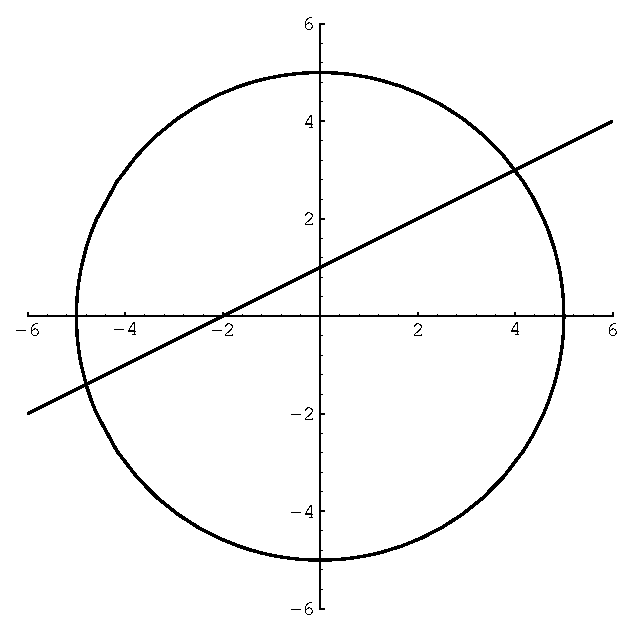
\includegraphics[width=3truein]{CircleLine}
\end{center}
\caption{Simple Algebraic Curves\label{Circle:Fig}}
\end{figure}

Let us start with the simplest type of geometric algebraic object, an
\keyi{algebraic curve}.  By an algebraic curve we mean a one-dimension
set of points whose coordinates satisfy an algebraic equation.  Two
simple examples of algebraic curves are shown in \figref{Circle:Fig},
where we have drawn a circle and straight line.  The points on the
circle are the zeroes of the polynomial $x^2 + y^2 - 25$, while the
line is the zeroes of $3y - x - 2$.  In particular we can define a
plane curve to be the set of zeroes of a polynomial in two variables.

Do the lines in \figref{Circle:Fig} constitute two curves or a single
curves?  It appears that it consists of two separate curves, one
superimposed on the other.  Nonetheless, there is a single polynomial
whose zeroes are the points in \figref{Circle:Fig}.  It is
\[
x^3 - 3 x^2 y + y^2 x - 3 y^3 + 2 x^2 + 2 y^2 - 25 x + 75 y + 50,
\]
which is the product of $x^2 + y^2 - 25$ and $3y - x - 2$.  We
probably want to say that the set of zeroes of an irreducible
polynomial is a single curve (or \keyi{irreducible curve}).

\begin{figure}
\begin{center}
  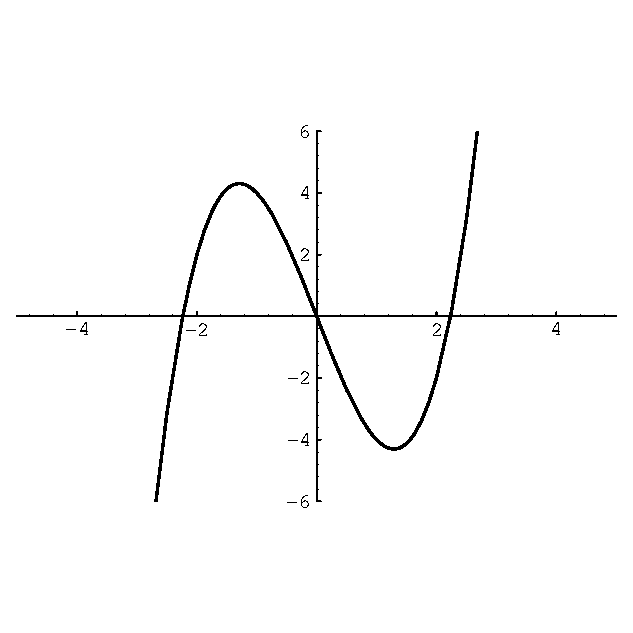
\includegraphics[width=1.5truein]{SimpleCubic1}
    \hfil 
  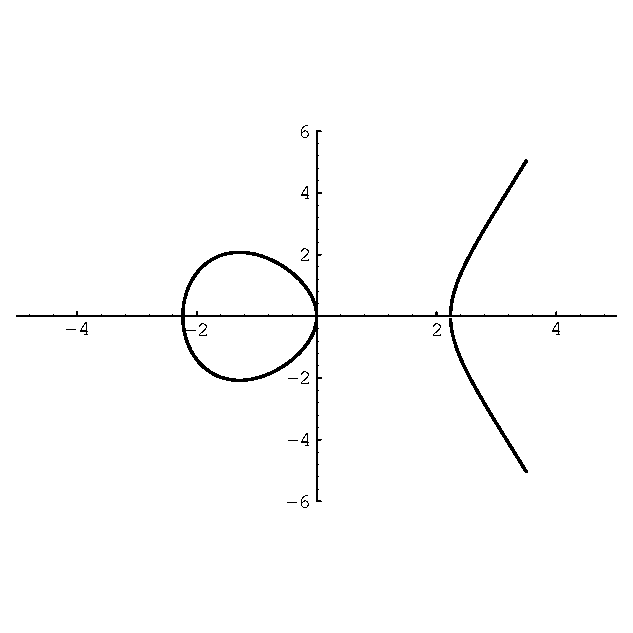
\includegraphics[width=1.5truein]{SimpleCubic2}
\end{center}
\caption{Cubic Curves: $y = x^3 - 5x$ and $y^2 = x^3 - 5x$}
\label{Simple:Cubic:Fig}
\end{figure}

Intuitively we think of the degree of an algebraic curve as the number of
times it can intersect a straight line.  For instance the curves in
\figref{Simple:Cubic:Fig} are obviously of degree three because each
intersects the $x$ axis at three places and no straight line can intersect
them more often.  Similarly the degree of the circle and straight line in
\figref{Circle:Fig} are 2 and 1 respectively.

Notice that a straight line can intersect a sine wave an infinite number of
times.  The sine wave is not an algebraic curve, if it was would have to be the
zeroes of a polynomial of infinite degree.  It is an example of a
transcendental curve.

The second curve of \figref{Simple:Cubic:Fig} is somewhat problematic.
It has two components, but the polynomial $y^2 - x^3 + 5x$ is
irreducible.  One way of looking at this curve is that it is generated
by taking the square roots of the values of $y$ in the
\figref{Simple:Cubic:Fig}(a).  Since there are two values of
$\sqrt{\alpha}$ for each value of $\alpha$, there are two values of
$y$ for each value of $x$ in \figref{Simple:Cubic:Fig}(b).  Notice
that the gap between the loop on the left and the curve on the right
at $x = \sqrt{5}$ arises because the the curve $x^3 - 5x$ is negative
in that region.  Thus the missing values actually lie in the complex
plane.

\begin{figure}
\begin{center}
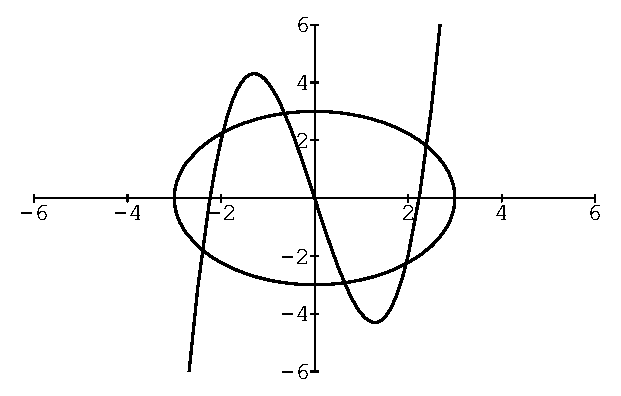
\includegraphics[width=3truein]{SimpIntersection}
\end{center}
\caption{Intersection of a Cubic and a Quadratic\label{Intersect:Fig}}
\end{figure}

Generalizing our observation on the intersection of curves and
straight lines, we would expect that the number of intersections of a
curve of degree $m$ and a curve of degree $n$ would be $mn$.  This is
illustrated by the curves in \figref{Intersect:Fig} where there are
six intersections.  Unfortunately is not always true.  Sometimes there
are fewer intersections.

\begin{figure}
\begin{center}
  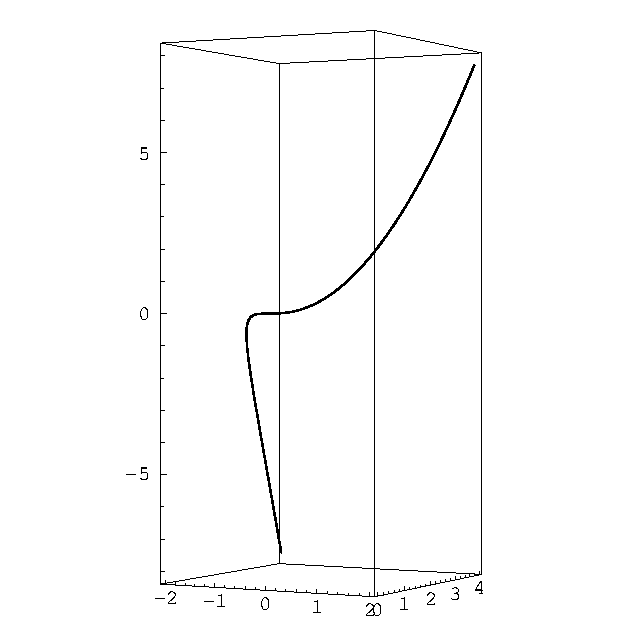
\includegraphics[width=1.5truein]{TwistedCubic1}
    \hfil 
  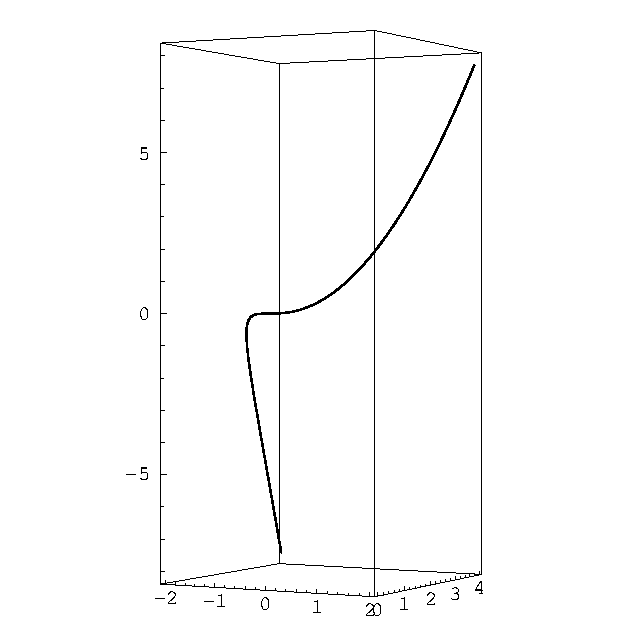
\includegraphics[width=1.5truein]{TwistedCubic2}
\end{center}
\caption{Twisted Cubic\label{Twisted:Cubic:Fig}}
\end{figure}
In three dimensions a single polynomial defines a surface.  In
general the intersection of two surfaces is a curve, although in
exceptional cases it could be a single point or a surface.  An example
of a curve in three dimensions is the \keyi{twisted cubic} shown in
\figref{Twisted:Cubic:Fig}.  This curve is the intersection of the surfaces
\[
y= x^2 \qquad \hbox{and}\qquad z=x^3.
\]
It is a fairly simple example of a curve that cannot be embedded in a
the plane.

\section{Commutative Algebra}

In the most general setting, we begin with a commutative ring $R$.  A
set of elements $I$ is chosen, and used to divide $R$ into equivalence
classes.  Two elements of $R$ are equivalent if their difference is in
$I$.  The set of equivalence classes is denoted by $R/I$.  We will
place restrictions on $I$ so that $R/I$ is still a ring.  For an
element to be equivalent to itself $0$ must be in $I$.  In fact, for
the relationship induced by $I$ to be an equivalence, $I$ must be an
additive group.  It is also not hard to see that if $i$ is an element
of $I$ and $a$ an element of $R$, then $ai$ must be an element of $I$.
Pick two elements of $R$, $r_1$ and $r_2$, such that $r_1 - r_2 = i$.
Since $r_1$ and $r_2$ are equivalent, we must have that $a r_1$ and
$ar_2$ are equivalent.  Thus, $$a r_1 - a r_2 = a \,(r_1 - r_2) = a i
\in I.$$ Sets that have these properties are called ideals.

\begin{definition}
Let $R$ be a commutative ring, and $I$ a subset of $R$.  If $I$ is an
additive group, and if $rI \subset I$ for all $r \in R$, then $I$ is
an \keyb{ideal}.
\end{definition}

\index{ideal, principal} \index{ideal, finitely generated}
In the integer case we used the set of multiples of an integer for
$I$.  The polynomial case described above used multiples of a single
polynomial $p(X)$.  Ideals that are multiples of a single element are
called {\em principal ideals\/}.  We have used the notation $(p)$ to
denote the set of multiples of $p$.  Generalizing this notation
slightly we will let $(a_1, a_2, \ldots, a_n)$ represent the set
\[
S = \{\, a_1 r_1 + a_2 r_2 + \cdots + a_n r_n 
        \mid r_1, r_2, \ldots, r_n \in R \,\}.
\]
$S$ is clearly an ideal. We say that $S$ is {\em generated} by $a_1,
a_2, \ldots, a_n$.  Since $S$ is generated by a finite number of
elements $S$ is called a {\em finitely generated ideal\/}.  There are
rings that have ideals which are not finitely generated, but we will
not discuss them here.  

All rings possess two ideals, the set consisting of the single element $0$
and the whole ring, $R$.  Notice that all the ideals of $R$ contain $(0)$
and are contained in $R$.  The residue class rings of these two ideals are
very dull ($R$ and zero ring) so most of our attention is confined to the
ideals between these two ``trivial'' ideals.

Recall that $\Z/(p)$ had no zero divisors if $p$ was a prime number.  In
fact $\Z/(p)$ is a field in this case.  We will extend
this definition to more general ideals.  Let $R$ be a ring, $I$ an ideal.
$I$ is a {\em prime ideal} if $R/I$ is an integral domain.  If $R/I$ is a
field then $I$ is a {\em maximal ideal\/}.  It is not difficult to see that
these characterizations are equivalent to standard definitions:

\begin{definition}
 $I$ is a \keyi{prime ideal} if for all elements $a$ and $b$
of $R$ such that $ab$ is an element of $I$, either $a$ or $b$ is an
element of $I$.
\end{definition}

\begin{definition}
$I$ is a \keyi{maximal ideal} if there is no ideal $J$ such that $I
\subset J$ other than $R$.
\end{definition}

All maximal ideals are prime.  For $\Z$ all prime ideals  are also maximal.
The situation is not always so simple.  If $R = \Z[X]$ there are three
classes of prime ideals: (p) where $p$ is a prime, $(f(X))$ where $f(X)$ is
an irreducible polynomial, and $(p, f(X))$ where $f(X)$ is irreducible
modulo $p$.  Only the third class leads to a field.

The set of prime ideals of a ring, $R$, is called the ring's
\keyi{spectrum}, $\Spec R$.  It is possible to put a topology on this
space called the \keyi{Zariski topology}.  The point of the space are then the
prime ideals.  Consider the ring $\Z[X]$.  Among the points in the
spectrum are the ideals generated by the linear polynomials $(X - a)$.
Thus there is a clear association between $\Z$ and a subset of the
points in $\Spec \Z$.  Similarly, there is an association between the
elements of $\Z \times \Z$ and the points of $\Spec \Z[X, Y]$.

Let $f$ be an element of $F[X]$, where $F$ is some field.  Let 
$\pger = (X - a)$ be a prime ideal of $F[X]$.  The residue of $f$ modulo
$\pger$ is $f(a)$.  In the spectrum of $F[X]$, the point $\pger$ is
associated with $a$ in $F$.  Thus it is natural to say that $f(a)$ is 
{\em the value of $f$ at $\pger$}.  More generally,
let $f$ be an element of some ring $R$ and $\pger$ a prime ideal of $R$.
The image of $f$ in $R/\pger$ is said to be the value of $f$ at $\pger$ and
is written $f(\pger)$ or $f_{\pger}$.

\medskip

\begin{definition}
A ring is said to be \keyi{Noetherian} if every ideal in the ring is
finitely generated.
\end{definition}

\begin{proposition}
Noetherian rings satisfy the descending chain condition.
\end{proposition}

\index{Hilbert Basis Theorem}
\begin{proposition}[Hilbert Basis Theorem] If $R$ is Noetherian then
$R[X]$ is also Noetherian.
\end{proposition}

\begin{proof}
Let $I$ be an ideal of $R[X]$.  The leading coefficients of the
elements of $I$ form an ideal in $R$ denoted by $\lc(I)$.  Since $R$
is noetherian $\lc(I)$ is finitely generated.  We will use this fact
to construct a basis for $I$.  Let $\{a_1, \ldots, a_n\}$ be a
generating set for $\lc(I)$.  Choose polynomials, $f_1, \ldots, f_n
\in I$ of smallest degree such that the leading coefficient of $f_i$
is $a_i$.  These polynomials generate an ideal $I' \subseteq I$.  Let
the maximum degree of any of the $f_i$ be $r$.  If $\deg f_i < r$,
replace $f$ by $X^{r -\deg f_i} f_i$ so that each of the $f_i$ is of
degree $r$.

We now show that the elements of $I$ are sums of elements of $I'$ and
polynomials of degree less than $r$.  Let $f = a X^m + \cdots$ be a
polynomial in $I$ but not $I'$, and assume $m \ge r$.  Since $\lc(I)$
is finitely generated, we can write $a$ as a linear combination of the
$a_i$
\[
a = c_1 a_1 + \cdots c_n a_n.
\]
The polynomial 
\[
g = X^{m-r} \left[ c_1 f_1 + \cdots c_n f_n \right]
\]
is an element of $I'$ and has the same leading term as $f$.  Repeating
this procedure with $f - g$ we can reduce $f$ to the sum of an element
in $I'$ and an element of $I$ of degree less than $r$.

Now we need to show that the elements of $I$ of degree less than $r$
are finitely generated.  Exactly the same technique is applied.  Let
$J_m$ denote the ideal of the leading coefficients of polynomials in
$I$ of degree $m$ and let $\{ f_{m1}, \ldots, f_{m n_m} \}$ be a set
of polynomials in $I$ of degree $m$ whose leading coefficients
generate $J_m$.  The finite set of polynomials $\{f_i \} \cap \{f_{ij}
\}$ generate $I$.

\end{proof}

The Hilbert Nullstellensatz.  Rabinowitsch's trick in \cite{Rabinowitsch1930-ww}.

\section{Ideal Theoretic Calculations}
\label{Ideal:Arith:Sec}

Given two orders $\ge_{x}$ and $\ge_{y}$ on monomials in $\vec X$ and
$\vec Y$ respectively, we can define an order on $\ge_{xy}$ by $\vec
X^{\vec a} \vec Y^{\vec b} \ge_{xy} \vec X^{\vec a'} \vec Y^{\vec b'}$
if $\vec X^{\vec a} \ge_{x} \vec X^{\vec a'}$ or $\vec X^{\vec a} =
\vec X^{\vec a'}$ and $\vec Y^{\vec b} \ge_{y} \vec Y^{\vec b'}$.

\begin{proposition}[Gianni-Trager-Zacharias]
\label{Lexical:Grobner:Prop}
Let $I$ be an ideal in $R[\vec X, \vec Y]$.  If $G \subset R[\vec X,
\vec Y]$ is a Gr\"obner basis for $I$ with respect to $\ge_{xy}$ then 
\begin{itemize}
\item $G$ is a Gr\"obner basis for $I$ with respect to the order
$\ge_x$ on $(R[\vec Y])[\vec X]$, the polynomial ring with coefficients
in $R[\vec Y]$.
\item $G\cap R[\vec Y]$ is a Gr\"obner basis for $I\cap R[y]$ with
respect to the order $\ge_{y}$.
\end{itemize}
\end{proposition}


\subsection{Ideal Arithmetic}
\label{Ideal:Arithmetic:Sec}

Compute intersection, quotient, dimension, localization of an ideal.

\subsection{Primary Decomposition}

\begin{proposition}[Gianni-Trager-Zacharias]
Let $I$ be a prime zero-dimensional ideal in $k[\vec X]$, 
\[
G = \{g_1(X_1, \ldots, X_n), g_2(X_2, \ldots, X_n), \ldots, g_n(X_n)\}
\]
a minimal Gr\"obner basis for $I$ with respect to $\lexord$.  Then for
almost all linear transformations of coordinates $g_i$ is linear in
$X_i$ for all $i$ less than $n$.
\end{proposition}

\begin{proof}
By the proof of the primitive element theorem, for almost all $a_1,
\ldots, a_n \in k$,
\[
R = k[\vec X]/I \simeq k[a_1 X_1 + \cdots + a_n X_n].
\]
If we choose new coordinates $Z_1, \ldots, Z_n$ such that 
\[
Z_n = a_1 X_1 + \cdots + a_n X_n
\]
then $R = k[Z_n]$.  Since $Z_i \in R$, $Z_i = f_i(Z_n)$ for some
polynomial $f_i$.
\end{proof}

\section{Special Case Lifting Techniques}




    %$Id: desingularization.tex,v 1.1 1992/05/10 19:38:30 rz Exp rz $
\chapter{Desingularization}
\label{Desing:Chap}


\section{Puiseux Series}
\label{Puiseux:Sec}

A paper on this is \cite{Cohn1984-zt}.

Original papers by Puiseux \cite{Puiseux1850-rf,Puiseux51}.


    %$Id: ratfun-decomp.tex,v 1.1 1992/05/10 19:38:20 rz Exp rz $
\chapter{Rational Function Decomposition}
\label{RatDecomp:Chap}

The problem of determining if a function can be written as the
composition of two ``smaller'' functions $f(x) = g(h(x))$ has been of
interest for a long time.  Although not every function can be
decomposed in this fashion, when such a decomposition does exist many
problems become significantly simpler.  For instance, if $f$ can be
decomposed into equal degree polynomials then its value at different
points can be computed with $O(\sqrt{n})$ multiplications rather than
with $O(n)$ multiplications, as is required in the general case.  In
addition, it is easier to determine if the zeroes of $f$ can be
expressed in terms of radicals if $f$ is decomposable

Until now, work has focused on the univariate, polynomial version of
this problem: When can the polynomial $f(x)$ be written as $g(h(x))$,
where both $g(x)$ and $h(x)$ are polynomials?  The original work in
the symbolic computation community was presented in 1976
\cite{Barton76}, but the algorithms, which in the worst case
required exponential time, were not published until 1985
\cite{Barton85}.  Soon afterward, Kozen and Landau
\cite{Kozen89} provided a polynomial time algorithm for
decomposition of polynomials over fields of characteristic zero that
did not require factorization of polynomials.  Some additional
improvements and an analysis of the positive characteristic case where
then presented by von zur Gathen \cite{Gathen87,Gathen90a}. A number
of other papers have since been published on different extensions and
variations of this problem
\cite{Alagar85,Gutierrez89,Dickerson89a,Dickerson89b}. 

The generalization to rational functions, which has significantly
wider applicability, appears to be a harder problem.  Notice that in
the polynomial case, the degree of $g$ and $h$ must divide the degree
of $f$.  This limits the number of different polynomials that must be
considered and allows one to solve the problem by looking for
solutions of non-linear algebraic equations (admittedly in exponential
time).  When $f$, $g$ and $h$ are rational functions, there is no
immediately obvious bound on the degrees of the numerators of $g$ and
$h$, since the numerator and denominator of $g(h(x))$ could have a
common factor.  In fact, no such common factor can arise, as we prove
below.

Furthermore, we demonstrate that for the rational function problem,
$g$ and $h$ can be determined from $f$ in polynomial time.  This new
algorithm is valid for univariate rational functions with coefficients
in any field over which one can factor polynomials.  Thus this
algorithm can also be used to find polynomial decompositions over
fields of positive characteristic, a problem that was not completely
resolved in earlier work.  Our algorithm requires the factorization of
a polynomial over an algebraic function field---although this can be
done in polynomial time it quite expensive.  Thus our technique is
significantly more costly than the earlier polynomial time algorithms
for the polynomial case, but is far more general.


A number of generalizations of polynomial decomposition are mentioned in
\cite{Barton85}, among which is rational function decomposition.
These generalizations appear to be somewhat {\em ad hoc} and no general
program was presented to guide future work.  This paper discusses a
natural framework, factoring of regular maps between varieties, into which
all previous generalizations of polynomial decomposition can be placed.  In
the one dimensional, univariate case, we develop a lattice of fields that
is in a one to one correspondence with the decomposition of rational
functions.  This result, combined with the subfield determination technique
of Landau and Miller \cite{Landau85b} and a few new ideas,
solves the problem of rational function decomposition over arbitrary fields.
We also present techniques for dealing with some problems from the general
framework.

In \sectref{Applications:Sec} we present two problems that illustrate
where functional decomposition problems arise.  A general frame for
discussion of functional decomposition problems is represented in 
\sectref{Vector:Framework:Sec}.  The mathematical sophistication used
in \sectref{Vector:Framework:Sec} is greater than elsewhere in
this paper, and the results presented there are only used
motivationally in the later sections.  Thus the reader may wish to
skip this section.

\sectref{Generalities:Sec} provides some general background material
about the types of fields that into our discussion of decompositions.
Existence and uniqueness of functional decompositions are
discussed in \sectref{Structural:Results:Sec}.
\sectref{Rational:Function:Decomposition:Sec} presents the new
algorithms for rational function decomposition.  We comment on
previous work and give some conclusions in
\sectref{Conclusions:Sec}.

Two appendices are included to make some fundamental material that is
used in the rational function decomposition algorithm more accessible.
Appendix~\ref{Factoring:Sec} discusses factorization of polynomials
over various rings in a way that we hope makes clearer the
contributions of various investigators.  This appendix was prompted by
an earlier reviewer's comment that factoring polynomials over
algebraic function fields must be harder than factoring over algebraic
number fields.

In Appendix~\ref{Subfield:Sec} we give a new presentation of Susan
Landau's techniques for determining subfields of algebraic extensions.
This work, which allows one to determine properties of the Galois
group of an separable algebraic extension without actually computing
the Galois group appears not to be well understood.  Our short summary
of the techniques and their justification thus seems necessary.



\section{Applications}
\label{Applications:Sec}

The original work on polynomial decomposition algorithms
\cite{Barton85} was motivated by the desire to obtain elementary 
techniques for expressing the zeroes of polynomials in terms of
radicals.  Our starting point was the well known technique for
reducing the degree of palindromic polynomials:
\[
\begin{aligned}
f(x) & = f_0x^{2n} + f_1 x^{2n-1} + \cdots + f_1 x + f_0, \\
     & =  x^n \left( f_0 \left(x + \frac{1}{x}\right)^n 
    + (f_1 - n f_0) \left(x + \frac{1}{x}\right)^{n-1} + \cdots \right), \\
     & = x^n g\left(x + \frac{1}{x}\right). 
\end{aligned}
\]
If $\alpha_1, \ldots, \alpha_n$ are the zeroes of $g(z)$ then the zeroes
of 
\[
x^2 - \alpha_i x + 1 = 0
\]
are the zeroes of $f(x)$.  Furthermore, if the $\alpha_i$ can be expressed
in terms radicals then so can the zeros of $f(x)$.

If $f(x)$ can be decomposed into two polynomials $f(x) =g(h(x))$, then the
zeroes of $f(x)$ are the zeroes of $h(x) = \alpha_i$ where the $\alpha_i$
are the zeroes of $g(x)$.  More generally, let $f(x)$ be decomposed into $f
= g_1 \circ g_2 \circ \cdots \circ g_r$.  If all of the $g_i$ are either
polynomials of degree less than $5$ or of the form $x^m$, then the zeroes
of $f(x)$ can be expressed in terms of radicals.

Within this context the obvious generalization is to the decomposition of
rational functions: When can a rational function be written as the
composition of two rational functions?  However, this doesn't directly
address the problem of solving equations in terms of radicals.  
The decomposition of $f(x)$ in the palindrome case can be written as
\[
f(x) = f_0 (x^2+1)^n + (f_1 - n f_0)(x^2+1)^{n-1} x + \cdots 
\]
So we have written $f(x)$ as $g(x^2+1, x)$, where $g(\cdot, \cdot)$ is
homogeneous and its degreee is half that of $f(x)$.  Thus a more
general question is When do there exist two univariate polynomials $h_1(x)$
and $h_2(x)$ and a homogeneous polynomial $g(x,y)$ such that $f(x) =
g(h_1(x), h_2(x))$?  Partial results have appeared in \cite{Weiss92}.

\medskip
Trager has pointed out another situation where a simple variant of
rational function decomposition naturally occurs.  Assume we wish to
integrate an indefinite integral of the form
\begin{equation}
\label{Integral:Radical:Eq}
\int A(x) \root p \of{B(x)} \, dx,
\end{equation}
where $A(x)$ and $B(x)$ are rational functions in $x$ over some field.
One approach is to determine if there is a rational function $R(x)$,
such that
\[
\int A(x) \root p \of{B(x)} \, dx = \int R(B(x)) \, d\root p \of{B(x)}
  = \int R(y^p) \, dy.
\]
Thus, if such a $R(y)$ can be found, the integral of
\eqnref{Integral:Radical:Eq} can be reduced to the easier problem of
integrating a rational function.  Such an $R(x)$ must satisfy the
functional equation:
\[
R(B(x)) = \frac{p A B}{B'}.
\]
So the integration of \eqnref{Integral:Radical:Eq} is reduced to the
question of when the function $A(x)/B'(x)$ can be written as a
rational function in $B$.

\section{A General Framework}
\label{Vector:Framework:Sec}

Though a number of generalization have been suggested for the
polynomial decomposition problem, they have not been put into a
coherent framework.  One of the main contributions of this paper is to
do just that.

Let $k$ be an {\em arbitrary} field.  The $n$-dimensional {\em affine
space} over $k$, which we denote by $\A^n(k)$, is the set of
$n$-tuples $(a_1, \ldots, a_n)$ where $a_i \in k$.  Two points in
$\A^n(k)$ are equal if and only if their components are equal.  The
$n$-dimensional {\em projective space}, denoted by $\P^n(k)$ is the
set of $n+1$ tuples $(a_0: a_1: \cdots : a_n)$ where the two tuples
$(a_0: a_1: \cdots : a_n)$ and $(b_0: b_1: \cdots : b_n)$ are equal if
there exists a non-zero $r \in k$ such that $r a_i = b_i$ for all $i$.
The colons in the representation indicate that the projective
equivalence relation is to be used.

A {\em regular map} $f: \A^n(k) \rightarrow \A^m(k)$ between two
affine spaces is a map that sends each point $(a_1, \ldots, a_n)$
to the point
\[
(f_1(a_1, \ldots, a_n), \ldots, f_m(a_1, \ldots, a_n)),
\]
where the $f_i$ are polynomials over $k$.  For projective spaces, a
map $f: \P^n(k) \rightarrow \P^m(k)$ is regular if
there are homogeneous polynomials $\{f_0, \ldots, f_m\}$ such that
\[
f : (a_0: a_1: \ldots: a_n) \mapsto 
   (f_0(a_0, \ldots, a_n): \ldots: f_m(a_0, \ldots, a_n)), 
\]
where the $f_i$ have the same total degree.

\begin{figure}
\[
\begin{diagram}
\node{\A^1(k)} \arrow[2]{e,t}{f} \arrow{se,t}{g} \node[2]{\A^1(k)} \\
\node[2]{\A^1{k}}\arrow{ne,t}{h} 
\end{diagram}
\]
\caption{Univariate Polynomial Factorization \label{Polynomial:Factor:Fig}}
\end{figure}

Let $X$ and $Z$ be two spaces (affine or projective) and let
$f:X\rightarrow Z$ be a regular map between them.  We claim that
the correct generalization of the polynomial decomposition problem is:
When does there exist a space $Y$ and regular maps $h:X\rightarrow
Y$ and $g:Y\rightarrow Z$ such that $f$ is equal to $g$ composed
with $h$?  We call this a {\em factorization} of the map $f$.  In this
paper we will be mostly concerned with the situation where $X$, $Y$
and $Z$ are the same spaces (the maps are endomorphisms).  The
simplest cases, endomorphisms of $\A^1(k)$ and $\P^1(k)$, are
precisely the polynomial and rational function decomposition problems.

\subsection{Endomorphisms of $\A^1(x)$ and $\P^1(k)$}
\label{Endo:A1:Sec}

The $X=Y=Z=\A^1(k)$ situation is illustrated in
\figref{Polynomial:Factor:Fig}.  For
$f$ to be regular there must be a univariate polynomial $f_p$ such
that $f$ sends $(x) \in \A^1(k)$ to $(f_p(x))$.  If $f_p(x)$ can be
decomposed into $g_p(h_p(x))$ then regular endomorphisms of $\A^1(k)$,
$g$ and $h$, can be constructed as in \figref{Polynomial:Factor:Fig}.
Conversely assume $f$ factors into $g$ and $h$.  Since all three maps
are regular, there exist corresponding polynomials $f_p$, $g_p$ and
$h_p$.  Since $f(x) = g(h(x))$, $f_p(x) = g_p(h_p(x))$.  

Rational function decomposition corresponds to the case when $X$, $Y$
and $Z$ are $\P^1(k)$, the projective line over some field.  The map
$(x,y) \mapsto (x/y)$ bijectively maps every point in the projective line,
except the ``point at infinity'' $(1, 0)$, to a point of $\A^1(k)$.
We will use this map to convert polynomial statements in projective
space into statements about rational functions.

Since $f$ is a regular endomorphism of $\P^1(k)$ then there exist
homogeneous polynomials $f_1$ and $f_2$ such that
\[
f : (x: y) \mapsto (f_1(x, y) : f_2(x, y)).
\]
For every point of $\P^1(k)$, except $(1 : 0)$, this map is equivalent to
the rational function
\[
f_r(z) = \frac{f_1(z, 1)}{f_2(z, 1)}
\]
where $(x : y) \mapsto (f_r(x/y) : 1)$.  Although $f_1(x, y)$ and
$f_2(x, y)$ have the same total degree, observe that $f_1(z, 1)$ and
$f_2(z, 1)$ need not have the same degree.  A rational function
\[
f_r(z) = \frac{p(z)}{q(z)} 
= \frac{p_{0} z^m + p_{1} z^{m-1} + \cdots + p_{m}}{q_0 z^n + q_1
z^{n-1} + \cdots + q_n}
\]
induces a regular endomorphism of $\P^1(k)$ as follows.  For
simplicity, assume $m > n$.  The point $(x, y) \mapsto (f_1(x, y),
f_2(x, y))$ where
\[
\begin{aligned}
f_1(x, y) &= y^m p\left(\frac{x}{y}\right) = p_0 x^m + p_1 x^{m-1} y +
\cdots + p_m y^m \\
f_2(x, y) &= y^m q\left(\frac{x}{y}\right) = q_0 x^n y^{m-n} + q_1 x^{n-1} y^{m-n+1} +
\cdots + q_m y^n 
\end{aligned}
\]

Now assume there are regular endomorphisms $g$ and $h$ (with similar
components) such that $f = g \circ h$.  Composing the maps, we have
\[
\begin{aligned}
f_1(x, y) & = g_1(h_1(x,y), h_2(x,y)), \\
f_2(x, y) & = g_2(h_1(x,y), h_2(x,y)).
\end{aligned}
\]
Formally write the quotient of these two equations:
\[
\begin{aligned}
\frac{f_1(x, y)}{f_2(x, y)} 
    & = \frac{g_1(h_1(x,y), h_2(x,y))}{g_2(h_1(x,y), h_2(x,y))}, \\
    & = \frac{g_1(\frac{h_1(x,y)}{h_2(x,y)},1)}{g_2(\frac{h_1(x,y)}{h_2(x,y)}, 1)},
\end{aligned}
\]
where the division by $h_2(x, y)$ is valid because $g_1$ and $g_2$
have the same total degree.  Or, writing $z = x/y$
\[
f_r(z) = \frac{f_1(z,1)}{f_2(z,1)} 
 = \frac{g_1(\frac{h_1(z,1)}{h_2(z,1)},1)}{g_2(\frac{h_1(z,1)}{h_2(z,1)}, 1)}
 = g_r(h_r(z)).
\]
Thus the factorization of an endomorphism of a projective line
generated by a rational function is equivalent to decomposition of the
rational function.

In this framework, the decomposition problems discussed in
\cite{Barton85,Alagar85,Gutierrez89,Gathen87} are equivalent to the
factorization of endomorphisms of $\A^1(\Q)$.  Kozen and Landau
\cite{Kozen89} and von zur Gathen \cite{Gathen90a,Gathen90b} consider
the morphism factorization problem for $\A^1(\F_q)$, but do not
provide polynomial time algorithms in all cases.  The multivariate
decomposition problem solved by Dickerson \cite{Dickerson89b} deals with endomorphisms of $\A^1(k[\vec x])$.

In this paper we give a polynomial time reduction of the endomorphism
factorization problem over $\P^1(k)$ to factorization of polynomials
over $k$.  As a special case this also resolves the problem for
$\A^1(k)$.

\subsection{Endomorphisms of $\A^n(k)$ and $\P^n(k)$}
\label{Endomorphism:An:Sec}

Within the framework of factoring regular maps, the natural
``multivariate'' generalization to consider is factorization of
endomorphisms of affine and projective spaces of higher dimension.
For instance, let $f$ be a regular endomorphism of the affine plane
$\A^2(k)$ and let $(a_1, a_2)$ be an element of $\A^2(k)$.
Then there are a pair of polynomials $f_1, f_2 \in k[x,y]$ such that 
\[
f(a_1, a_2) = (f_1(a_1, a_2), f_2(a_1, a_2)).
\]
If $f$ factors into two maps $g$ and $h$, $f = g \circ h$, then the
polynomial components of $g$ and $h$ satisfy:
\begin{equation}\label{2D:Affine:Decomp:Eq}
\begin{aligned}
f_1(x, y) & = g_1(h_1(x, y), h_2(x, y)), \\
f_2(x, y) & = g_2(h_1(x, y), h_2(x, y)).
\end{aligned}
\end{equation}

A regular endomorphism of $\P^2(k)$ is a triple of co-prime homogeneous
polynomials
\[
(f_1(x,y,z): f_2(x,y,z): f_3(x,y,z)).
\]
If $g$ and $h$ are also regular endomorphisms such that $f = g \circ
h$ then 
\[
(f_1 : f_2 : f_3) =
 (g_1(h_1, h_2, h_3) : g_2(h_1,h_2,h_3) : g_3(h_1, h_2, h_3)).
\]
Since $(x:y:z) \in \P^2(k)$ and the polynomials are homogeneous, we can
rewrite this as
\[
\begin{aligned}
  \frac{f_1(x,y,1)}{f_3(x,y,1)} & 
   = \frac{g_1(\frac{h_1(x,y,1)}{h_3(x,y,1)},\frac{h_2(x,y,1)}{h_3(x,y,1)},1)}
          {g_3(\frac{h_1(x,y,1)}{h_3(x,y,1)},\frac{h_2(x,y,1)}{h_3(x,y,1)},1)},\\
  \frac{f_2(x,y,1)}{f_3(x,y,1)} & 
   = \frac{g_2(\frac{h_1(x,y,1)}{h_3(x,y,1)},\frac{h_2(x,y,1)}{h_3(x,y,1)},1)}
          {g_3(\frac{h_1(x,y,1)}{h_3(x,y,1)},\frac{h_2(x,y,1)}{h_3(x,y,1)},1)}.
\end{aligned}
\]
Identifying the rational functions $F_i(x,y)$ with $f_i/f_3$ and
similarly for $G_i$ and $H_i$ we have
\begin{equation}\label{2D:Projective:Decomp:Eq}
\begin{aligned}
F_1(x, y) & = G_1(H_1(x, y), H_2(x, y)), \\
F_2(x, y) & = G_2(H_1(x, y), H_2(x, y)).
\end{aligned}
\end{equation}
Comparing \eqnref{2D:Affine:Decomp:Eq} with
\eqnref{2D:Projective:Decomp:Eq} we see that passing from
endomorphisms of $\A^2(k)$ to endomorphims of $\P^2(k)$ converts the
bivariate polynomial decomposition problem to the corresponding
rational function decomposition problem.  These higher dimensional
endomorphism problems are much harder than the one dimensional problem
of \sectref{Endo:A1:Sec}.


\subsection{Endomorphisms of Curves}
\label{Endo:Curves:Sec}

In addition to dealing with endomorphism of $\A^n$ and $\P^n$ we can
discuss endomorphisms of other algebraic structures, like algebraic
curves.  Perhaps the most interesting class of curves from this
perspective are elliptic curves such as
\[
E: y^2 = x^3 - x,
\]
which in projective space has a huge number of endomorphisms.  For
instance, 
\[
(x:y:z) \mapsto (2(x^2+z^2)^2 : x^6-5x^4 z^2 - 5 x^2 z^4 + z^6 :
  (8x^3 - 8 x)y).
\]
For simplicity, we write these maps as rational functions, allowing us to
drop the third coordinate.  The previous endomorphism is then
\begin{equation} \label{Double:Endo:Eq}
(x, y) \mapsto \left( \frac{x^4+2x^2+1}{4x^3-4x}, 
  \frac{x^6-5x^4-5x^2+1}{8(x^3-x)^2}y\right).
\end{equation}
All endomorphisms of elliptic curves are of the form $(p(x), q(x)
y)$, where $p(x)$ and $q(x)$ are rational functions.  

Points on an elliptic curve obey a group law
\cite{SilvermanJH86}.  If $P_i = (x_i, y_i)$ are points on
the elliptic curve $E_{a,b} : y^2 = x^3+ax+b$ then $P_3 = P_1 + P_2$
when
\[
\lambda = \left\{\begin{array}{ll}
  \displaystyle\frac{y_2 - y_1}{x_2 - x_1} & \mbox{if $P_1 \not= P_2$}\\
  \displaystyle\frac{3x_1^2+a}{2y_1} & \mbox{if $P_1 = P_2$}
 \end{array}\right.
\]
and
\[
\begin{aligned}
  x_3 & = - (x_1 + x_2) + \lambda^2, \\ 
  y_3 & = -y_1 - \lambda (x_3 - x_1).
\end{aligned}
\]
The endomorphism \eqnref{Double:Endo:Eq} sends
$P_1\mapsto P_1 + P_1 = 2P_1$, which is denoted by $[2]$.  Similarly,
we can generate endomorphisms corresponding to multiplication by any
positive number $[n]$.  The additive inverse of $P_1 = (x_1, y_1)$ is
$(x_1, - y_1)$, so we have 
\[
[-1] : (x, y) \mapsto (x, - y),
\]
and thus we have an endomorphism of $E_{a,b}$ for each element of
$\Z$.

In addition there are occasionally additional endomorphims.  For
instance, the map 
\[
[i] : (x, y) \mapsto (-x, iy)
\]
is an endomorphism of $y^2 = x^3 -x$.  Clearly, $[i] \circ [i] =
[-1]$.  Using the additional formula given above, we can compute the
endomorphism $[1+i]$:
\[
[1+i] : (x, y) \mapsto \left(-\frac{i}{2}\left(x - \frac{1}{x}\right),
  -\frac{1+i}{4}\left(1 + \frac{1}{x^2}\right) y\right).
\]
Composing $[1+i]$ with itself we have
\[
\begin{aligned}
\relax [1+i]\circ[1+i](x,y) & = \left(
-\frac{x^4+2x^2+1}{4x^3-4x}, \frac{i(x^6-5x^4-5x^2+1)}{8(x^3-x)^2}y\right)\\
& = [i] \circ [2] (x,y).
\end{aligned}
\]
In fact there is an isomorphism between $\End(E_{-1,0})$ and $\Z[i]$.

\section{Preliminaries}
\label{Generalities:Sec}

\subsection{Geometry}
The geometric formulation of the decomposition problem leads very
naturally discussed in \sectref{Vector:Framework:Sec} lead very
naturally to the algebraic problems that are resolved in the body of
this paper. 

Let $X$ be an affine variety embedded in $\A^n(k)$.  Recall that the
ideal of $X$ is $I(X) \subseteq k[x_1, \ldots, x_n]$, the set of all
polynomials that vanish on $X$.  The {\em coordinate ring} of $X$,
$\Gamma(X)$, is defined to be $k[x_1, \ldots, x_n]/I(X)$.  The
elements of the coordinate ring can be identified with the polynomial
functions from $X$ to $k$.  Notice that when $X = \A^1(k)$, $\Gamma(X)
= k[x_1]$.  The quotient field of the coordinate ring $\Gamma(X)$ is
called the {\em function field} of $X$ and is denoted by $K(X)$.  For
$X=\A^1(k)$, $K(X) = k(x_1)$.

A polynomial map $f: X \rightarrow Z$ induces a homomorphism between
between coordinate rings, $f^{\ast}: \Gamma(Z) \rightarrow
\Gamma(X)$, as follows.  Let $p$ be an element of $\Gamma(Z)$, then $p$ is a
polynomial from $Z$ to $k$.  $f^{\ast}(p)$ is the polynomial map from
$X$ to $k$ defined by $f^{\ast}(p) = p \circ f$.  This homomorphism
can be canonically extended to one between function fields:
$f^{\ast}:K(Z) \rightarrow K(Z)$.  When $X$ and $Z$ are
irreducible, have the same dimension and $f(X)$ is dense in $Z$ then
$K(X)$ is an algebraic extension of $f^{\ast} K(Z)$.  ($\A^n(k)$ and
$\P^n(k)$ are irreducible and both have dimension $n$.)

\begin{figure}
\[
\begin{diagram}
\node{X} \arrow[2]{e,t}{f} \arrow{se,t}{g} \node[2]{Z} \\
\node[2]{Y}\arrow{ne,t}{h} 
\end{diagram}
\]
\caption{Morphism Factorization \label{Morphism:Factorization:Fig}}
\end{figure}

For example let $X = Z = \A^1(k)$ and let $f : X \rightarrow Z$ be
a map such that $(a_1) \mapsto (a_1^2) \in Z$.  The coordinate rings
of $X$ and $Z$ are both $k[x] = \Gamma(X) = \Gamma(Z)$.  Let $p(x) =
x^3+x$ be an element of $\Gamma(Z)$, then $f^{\ast}(p) = p \circ f =
x^6+x^2$. Furthermore, $f^{\ast}(\Gamma(Z)) = k[x^2] \subseteq
\Gamma(X)$.  Passing to the function fields, we see that $f^{\ast}K(Z)
= k(x^2)$ and $K(X) = k(x)$.

The relationship between $f^{\ast}K(Z)$ and $K(X)$ is the key to
understanding the behavior of morphism under composition and thus
generalizations of the polynomial decomposition problem.  Consider, for
instance, a factorization of $F$ as indicated in
\figref{Morphism:Factorization:Fig}.  The previous discussion shows
that both $h^{\ast}K(Y)$ and $f^{\ast}K(Z)$ are subfields of $K(X)$
and that $g^{\ast}K(Z)$ is a subfield of $K(Y)$.  This gives the
field structure indicated in \figref{Variety:Structures:Fig}.

\begin{figure}
\[
\begin{diagram}
\node{K(X)} \arrow{s,,-} \\
\node{h^{\ast}K(Y)} \arrow{e,t}{k^{\ast}} \arrow{s,,-} \node{K(Y)} \arrow{s,,-}\\
\node{f^{\ast}K(Z)} \arrow{e,t}{h^{\ast}} \node{g^{\ast} K(Y)}
\end{diagram}
\]
\caption{Fields involved in decomposition \label{Variety:Structures:Fig}}
\end{figure}

A finite morphism $f:X \rightarrow Z$ has a non-trivial
factorization if and only if there is an intermediate field between
$K(X)$ and $f^{\ast}K(Z)$.  Once such an intermediate field is found,
it is still necessary to reconstruct $g$, $h$ and $Y$ from it.  This
can be quite difficult.

\subsection{Field Structure}
We need to use fields that have a rather unusual presentation,
$k(f(x))$ where $f(x)$ is a rational function.  For example, the field
$k(x^2)$ is the field of rational functions in $x^2$, \eg,
\[
\frac{x^4 + x^2 + 1}{x^4 + 1} \in k(x^2),
\]
but $x$ and $x^2 + x$ are not elements of $k(x^2)$.  There is an
isomorphism between $k(x^2)$ and $k(t)$, with $x^2 \mapsto t$.
At the same time, however, $k(x^2)$ can be embedded in $k(x)$ by $x^2
\mapsto x^2$.  Since $k(x^2)$ and $k(x)$ both have transcendence
degree $1$ over $k$ and $k(x^2) \varsubsetneq k(x)$, $k(x)$
must be an algebraic extension of $k(x^2) = k(t)$.  In fact, $x =
\sqrt{t} =\sqrt{(x^2)}$, so the algebraic degree of $k(x)$ over
$k(x^2)$ is $2$.  The following diagram illustrates this.
\[
\begin{diagram}
\node{k(x)} \arrow{s,,-}\arrow{e,t,-}{\cong}
  \node{E[\alpha]/(\alpha^2-t)} \arrow{s,,-} \\
\node{k(x^2)} \arrow{e,t,-}{\cong} \node{E=k(t)}
\end{diagram}
\]
Each of the horizontal lines are isomorphisms.  At the bottom we have
$x^2 \mapsto t$, while the top line is $x \mapsto \alpha$.

Let $p(x)$ be a polynomial over $k$ and denote by $k(p(x))$ the field
of rational functions in $p(x)$.  Using the same notation as the in
the diagram above, the minimal polynomial for $\alpha$, which
generates $k(x)$ over $k(p(x))$, is $p(\alpha) -
t$.  Since this polynomial is linear in $t$, it is irreducible and
the degree of the polynomial $p$ is the algebraic degree of $k(x)$
over $k(p(x))$.

More generally, if $f(x)$ is a rational function over $k$, $k(f(x))$
is the field of rational functions in $f(x)$.  We extend the notion of
degree of a polynomial by defining the {\em degree} of a rational
function $f(x)$, also denoted 
by $\deg f$, to be the maximum of the polynomial degrees of the
(relatively prime) numerator and denominator of $f$.  For polynomials,
the degree of the field $k(x)$ over $k(f(x))$ was shown to be the
degree of $f$.  This is also true for rational function, as shown by
the following proposition.

\begin{proposition}
\label{Luroth:Extension:Degree:Prop}
Let $k(x)$ be an extension of the field $k(f(x))$ where $f(x)$ is a
rational function of degree $n$.  Then $\fieldDegree{k(x)}{k(f(x))} = n$.
\end{proposition}

\begin{proof}
Denote the numerator of $f(x)$ by $p(x)$ and the denominator by
$q(x)$.  Without loss of generality we can assume that $p$ and $q$ are
relatively prime.
We can consider instead the isomorphic fields $k(t) \cong
k(f(x))$ as the ground field, and
\[
k(t)[x]/(p(x) - t q(x)) \cong k(x)
\]
as an algebraic extension of $k(t)$.  $P(x,t) = p(x) -t q(x)$ is primitive
as a polynomial in $t$ since $p(x)$ and $q(x)$ are relatively prime.  Since
it is linear in $t$ it is irreducible.  Therefore, the degree of $x$ over
the field $k(t)$ is
\[
\deg_{x} P(x,t) = \max( \deg p, \deg q) = \deg f.
\]
\end{proof}

\noindent
Notice that $k(x)$ is integral over $k(f(x))$ if and only if $f(x)$ is
a polynomial.

An extremely important tool in this study is the following proposition
on the degree of the composition of two rational functions.  It is
clear for polynomials that the degree of $g\circ h$ is the product of
$\deg g$ and $\deg h$.  The following proposition shows that this is
also true for rational functions.  This proposition is well known in
mathematical circles.  See the comment after definition 1 in
\cite{Fried74}. 

\begin{figure}
\[
\begin{diagram}
\node{k(x)} \arrow{s,,-} \\
\node{k(h(x))} \arrow{e,t}{\varphi_h} \arrow{s,,-} \node{k(y)} \arrow{s,,-}\\
\node{k(f(x))} \arrow{e,t}{\varphi_h} \node{k(g(y))}
\end{diagram}
\]
\caption{Fields involved in decomposition \label{Bound:Field:Fig}}
\end{figure}

\begin{proposition}
\label{RatDecomp:Bound:Prop}  Let $k$ be an arbitrary field, and 
assume $f(x)$, $g(x)$ and $h(x)$ are elements of $k(x)$ such that
$f(x) = g(h(x))$.  Then
\[
\deg f = (\deg g) \cdot (\deg h)
\]
\end{proposition}

\begin{proof}
Consider the fields shown in \figref{Bound:Field:Fig}.  The map
$\varphi_h : y \mapsto h(x)$ is an isomorphism of $k(y)$ onto
$k(h(x))$ and restricted to $k(g(y))$ it yields an isomorphism of
$k(g(y))$ onto $k(f(x))$.

By \propref{Luroth:Extension:Degree:Prop}, the degree of each of
the extensions is
\[
\begin{aligned}
\fieldDegree{k(x)}{k(h(x))} & = \deg h, \\
\fieldDegree{k(x)}{k(f(x))} & = \deg f, \\
\fieldDegree{k(y)}{k(g(y))} & = \deg g. 
\end{aligned}
\]
$k(h(x))$ is an algebraic extension of $k(f(x))$ inside $k(x)$.  Thus,
\[
\begin{aligned}
  \deg f = \fieldDegree{k(x)}{k(f(x))} & = \fieldDegree{k(x)}{k(h(x))}
      \cdot \fieldDegree{k(h(x))}{k(f(x))} \\
    & =\fieldDegree{k(x)}{k(h(x))} \cdot \fieldDegree{k(y)}{k(g(y))} 
      = (\deg h) \cdot (\deg g).
\end{aligned}
\]
\end{proof}

\medskip
The lattice structure of fields of the form $k(f(x))$ is central to
our study of functional decomposition.  There are four basic questions
whose resolution would clarify this lattice structure:
\begin{itemize}
\item[{\bf A}] When is $k(f_1(x)) \subseteq k(f_2(x))$?
\item[{\bf B}] When is $k(f_1(x))$ equal to $k(f_2(x))$?
\item[{\bf C}] Can we explicitly represent $k(f_1(x), f_2(x))$, the smallest
field containing $k(f_1(x)) \cup k(f_2(x))$?
\item[{\bf D}] Can we explicitly represent $k(f_1(x)) \cap k(f_2(x))$?
\end{itemize}
Questions {\bf A} and {\bf B} are relatively easy and are answered
below.  Question {\bf C} is not difficult, but our solution requires
L\"uroth's theorem and is discussed a bit later.  The final question
seems somewhat difficult.  We do not have a complete answer at this
time.

We begin with the first question.  If there exists a rational function
$g(x)$ with coefficients in $k$ such that $f_1(x) = g(f_2(x))$, then
$f_1(x)$ will be an element of $k(f_2(x))$ and each element of
$k(f_1(x))$ will be an element of $k(f_2(x))$.  Conversely, if
$f_1(x)$ is in $k(f_2(x))$ then there must exist a rational function
$g(x)$ such that $f_1(x) = g(f_2(x))$.  Thus we have the following
proposition, which also appears in Weber \cite{Weber:Algebra:II},
\S$126$.

\begin{proposition} \label{Luroth:Subfield:Prop}
$k(f_1(x)) \subseteq k(f_2(x))$ if and only if there exists a rational
function $g(x) \in k(x)$ such that $f_1(x) = g(f_2(x))$.
\end{proposition}

If two fields $k(f_1(x))$ and $k(f_2(x))$ are equal then by the
\propref{Luroth:Subfield:Prop}, there exist rational functions $\lambda_1(x)$ and
$\lambda_2(x)$ such that
\[
\begin{aligned}
f_1(x) & = \lambda_1(f_2(x))\quad \mbox{and}\\
f_2(x) & = \lambda_2(f_1(x)),
\end{aligned}
\]
which means that
\[
f_1(x) = \lambda_1(\lambda_2(f_1(x)))
\]
or $\lambda_1(\lambda_2(x)) = x$.  Applying
\propref{RatDecomp:Bound:Prop} we see that 
\[
(\deg \lambda_1) \cdot (\deg \lambda_2) = 1.
\]
Since the degree of a rational function is a non-negative integer, the
only rational functions that can have inverse are those that are the
ratio of two linear polynomials.  

Such a rational function is called a {\em fractional linear} function:
\[
\lambda(x) = \frac{a x + b}{c x + d}.
\]
If either $cx+d$ divides $ax+b$ or $a=c=0$ then the degree of
$\lambda(x)$ will be $0$.  Such fractional linear function is called
{\em degenerate\/}.  In the first case,
\[
\frac{a}{c} = \frac{b}{d},
\]
or $ad - bc = 0$.  In the second case, $a=c=0$, $ad -bc$ is also zero.
Thus a necessary a sufficient condition for $\lambda(x)$ to have
degree $1$ is that $ad-bc \not=0$.  

If a fractional linear function is not degenerate then its inverse
under composition is
\[
\lambda^{-1}(x) = \frac{-dx + b}{cx - a}.
\]
Thus we have the following proposition, which answers our second
fundamental question.

\begin{proposition}\label{Bilinear:Inverse:Prop}
If $k(x)$ is equal to $k(y)$ then there exists a fractional linear
function $\lambda$ with coefficients in $k$ such that $x =
\lambda(y)$.  In particular, if $k(f_1(x))$ is equal to $k(f_2(x))$
then there exists a bilinear function $\lambda$ such that $f_1(x) =
\lambda(f_2(x))$ and $f_2(x) = \lambda^{-1}(f_1(x))$.
\end{proposition}

If $f(x) = g(h(x))$ then \propref{RatDecomp:Bound:Prop} provides
bounds on the degrees of $g(x)$ and $h(x)$ in terms of the degree of
$f(x)$.  Thus in principal we have an algorithm for rational function
decomposition: Set up a system of algebraic equations in the
undetermined coefficients of $g$ and $h$.  Any solution to the system
in $k$ will yield a decomposition of $f(x)$.  This algorithm is
exponential time.  In \sectref{Rational:Function:Decomposition:Sec} we
present efficient algorithms.

\medskip
The link between field structure and rational function decomposition
comes from {\em L\"uroth's theorem\/}, which was proven by L\"uroth
\cite{Luroth76} for $k = \C$ and by Steinitz in general
\cite{Steinitz10}.

\begin{proposition}[L\"uroth]
\label{Luroths:Prop}
If $k \varsubsetneq K \subset k(x)$ then $K = k(g(x))$ where $g(x)$ is
a rational function in $x$.
\end{proposition}

\noindent
An elementary proof of L\"uroth's theorem may be found in van der
Waerden \cite{Waerden:Algebra}.  An effective proof appears in
Weber \cite{Weber:Algebra:II} \S$124$, and in English in Schinzel
\cite{Schinzel:Polynomials}.

L\"uroth's theorem says that each field in the lattice of subfields
between $k(x)$ and $k$ that has transcendence degree $1$ over $k$
is generated by a single rational function.  In particular, $k(f_1(x),
f_2(x)) = k(h(x))$ for some rational function $h(x)$ and either
$k(f_1(x)) \cap k(f_2(x)) = k(g(x))$ for some rational function $g(x)$
or their intersection is $k$.  We will show, for instance that
$k(x^2+1)\cap k(x^3+1) = k$ in \sectref{Decomposition:Uniqueness:Sec}. 

Using L\"uroth's theorem question {\bf C} can be addressed
straightforwardly.  We have the following sequence of fields:
\[
k(x) \supseteq k(f_1(x), f_2(x)) \supseteq k(f_1(x)),
\]
where both $k(x)$ and $k(f_1(x), f_2(x))$ are algebraic extensions of
$k(f_1(x))$.  In particular $x \in k(x)$ is algebraic over
$k(f_1(x))$.  To make this more explicit we write $k(f_1(x)) = k(t)$
and
\[
k(x) = k(t)[\alpha]/(p(\alpha)),
\]
where $p(\alpha)$ is the minimal polynomial of $x$ over $k(f_1(x))$,
\ie,
\[
p(Z) = \num (f_1(Z) - t) = \num f_1(Z) - t \den f_2(Z).
\]
In terms of $\alpha$, $k(f_1(x), f_2(x)) = k(t)[f_2(\alpha)]$.  
$f_2(\alpha)$ is a zero of the polynomial
\[
\prod_{f_1(\alpha_i) = 0} \left(Z - f_2(\alpha_i)\right) = q(t, Z),
\]
where the product is over the zeroes of $f_1(Z)$.  The coefficients of
$q(t, Z)$ lie in $k$.  It can be computed using resultants as
\[
q(t, Z) = \Norm_{k(x)/k(f_1(x))} Z - f_2(\alpha) 
        = \res_u (f_1(u), Z- f_2(u)).
\]
By \propref{Sqfr:Norm:Prop}, $q(t, Z)$ is the power of an irreducible
polynomials, which we denote by by $Q(t, Z)$.  $Q(t, Z)$ can be
computed by taking the GCD of $q(t, Z)$ and $q_Z(t,Z)$ or explicitly
computing the $r$\th{} roots of $q(t,Z)$, where $r$ divides the degree
of $q(t,Z)$.nn

Any zero of $q(t, Z)$ (or $Q(t,Z)$) generates $k(f_1(x), f_2(x)) =
k(h(x))$.  Further, by L\"uroth's theorem such a zero must be a
rational function in $x$.  Thus $Z - h(x)$ must divide $q(f_1(x), Z)$.
So $h(x)$ can be obtained by examining a linear factor of the
$q(f_1(x), Z)$.

\subsection{Normal Subfields of $k(x)$}
\label{Normal:Subfields:Sec}

If $E$ is a subfield of $k(x)$, then we call it a {\em normal
subfield} if $k(x)/E$ is a normal extension.  By L\"uroth's theorem we
know that all subfields of $k(x)$ are of the form $k(g(x))$ for some
$g(x)$, or $k$.  It is also interesting to find out which of those subfields
are normal subfields.  As we shall see, if $k(x)/k(g(x))$ is normal
then $g(x)$ has some very interesting properties.

Since $k(x)/k$ is not an algebraic extension, the only normal
subfields are finite degree subfields of $k(x)$.  By
\propref{Bilinear:Inverse:Prop} the only automorphisms of $k(x)$ are
those that send
\[
x \mapsto \frac{ax+b}{cx+d}.
\]
The set of such automorphisms is isomorphic to the group
$\mbox{SL}_2(k)/\{\pm I\}$ of $2\times 2$ matrices with determinant
equal to $1$.  If $k(x)$ is normal over $E$, then the Galois group of
$k(x)/E$ must be a finite subgroup of $\mbox{SL}_2(k)/\{\pm I\}$.
Thus the problem of determining all normal subfields of $k(x)$ is
equivalent to finding all normal subgroups of $\mbox{SL}_2(k)/\{\pm
I\}$.

The study of the finite subgroups of $\mbox{SL}_2(\C)/\{\pm I \}$ has
a long history.  Any finite subgroup corresponds to a rotation or
reflection of the Riemann sphere, so the finite subgroups correspond
to the regular solids in three dimensions and date back to the Greeks.

Klein \cite{Klein75} gave the first modern, geometric proof that there
were only finitely many subgroups of $\mbox{SL}_2(\C)/\{\pm I\}$.  In
the context of monodromy groups of differential equations, Jordan
\cite{Jordan76} gave a proof using Sylow groups.  He extended
this work to the finite subgroups of $\mbox{SL}_2(\C)/\{\pm I\}$ in
\cite{Jordan:1878}.  Gordan \cite{Gordan77} considered these groups
from the perspective of invariant theory.  A good discussion is in
\cite{Klein56}.

\begin{proposition}[Klein] \label{Klein:Groups:Prop}
The finite subgroups of $\mbox{SL}_2(\C)/\{\pm I \}$ are of one of the
following five types:
\begin{itemize}
\item $C_n$, the cyclic group of order $n$;
\item $D_n$, the dihedral group of order $n$;
\item $A_4$, the alternating group on four letters or tetrahedral group;
\item $S_4$, the symmetric group on four letters or octahedral group;
\item $A_5$, the alternating group on five letters or icosahedral group.
\end{itemize}
\end{proposition}

The elements of these groups, as subgroups of $\mbox{SL}_2(k)/\{\pm I\}$ are as
follows.  The elements of the cyclic group are:
\[
C_n = \left\{\zeta_n z \right\}.
\]

For the dihedral group, the elements are:
\[
D_n = \left\{ \zeta_n z, \frac{1}{\zeta_n z} \right\}
\]

For the tetrahedral group:
\[
\left\{
 \pm z, \pm \frac{i}{z}, 
 \pm \frac{(1+i)z + \sqrt{2}}{\sqrt{2}z - 1 + i},
 \pm \frac{\sqrt{2}z - 1 + i}{(1+i)z + \sqrt{2}},
 \pm \frac{(1-i)z + \sqrt{2}}{\sqrt{2}z - 1 - i},
 \pm \frac{\sqrt{2}z - 1 - i}{(1-i)z + \sqrt{2}}
\right\}
\]

The octahedral group has two different representations:
\[
\left\{
 i^k z, \frac{i^k}{z}, 
 i^k\frac{z+1}{z-1}, i^k\frac{z-1}{z+1}, 
i^k\frac{z+i}{z-i}, i^k\frac{z-i}{z+i}
\right\}
\]
and
\[
\left\{
  i^k z, \frac{i^k}{z}, 
 i^k \frac{(1+i)z + \sqrt{2}}{\sqrt{2}z - 1 + i},
 i^k \frac{\sqrt{2}z - 1 + i}{(1+i)z + \sqrt{2}},
 i^k \frac{(1-i)z + \sqrt{2}}{\sqrt{2}z - 1 - i},
 i^k \frac{\sqrt{2}z - 1 - i}{(1-i)z + \sqrt{2}}
\right\}
\]
where $k = 0, 1, 2, 3$.

And for the icosahedral group:
\[
\left\{
  \zeta_5^{\mu} z, - \frac{1}{\zeta_5^{\mu} z},
  \zeta_5^{\nu} 
   \frac{-(\zeta_5-\zeta_5^4)\zeta_5^\mu z + \zeta_5^2-z\zeta_5^3}
        {(\zeta_5^2-\zeta_5^3)\zeta_5^\mu z + \zeta_5 - \zeta_5^4},
  -\frac{1}{\zeta_5^{\nu}}
   \frac{(\zeta_5^2-\zeta_5^3)\zeta_5^\mu z + \zeta_5 - \zeta_5^4}
        {-(\zeta_5-\zeta_5^4)\zeta_5^\mu z + \zeta_5^2-z\zeta_5^3}
\right\}
\]



\begin{proposition}[Klein] \label{Klein:Fields:Prop}
Let $k$ be a field of characteristic zero and $k(t)$ a transcendental
extension of $k$, and assume that $k$ contains sufficiently many roots
of unity.  If $E$ is a normal subfield of $k(t)$ then it is isomorphic
to one of the following fields:
\begin{itemize}
\item $k(t^n)$ for some positive integer $n$;
\item $k(t^n + \zeta_n t^{-n})$, where $\zeta_n$ is an $n$\th{} root
of unity. 
% \item $k\left(\frac{(t^2+a)^2}{t(t^2-2bc^{-1}t-a)}\right)$ where
% $a,b,c \in k$, $ac\not= 0$ and $b^2+ac^2=1$.
\item $k\left(\frac{t^{12}-33t^8-33t^4+1}{t^2(t^4-1)^2}\right)$;
\item $k\left(\frac{(t^{12}-33t^8-33t^4+1)^2}{t^4(t^4-1)^4}\right)$;
\item $k\left(\frac{(t^{20}-228t^{15}+494t^{10}+228t^5+1)^3}{t^5(t^{10}+11t^5-1)^5}\right)$.
\end{itemize}
\end{proposition}



\subsection{Examples}
\label{Field:Examples:Sec}
One of the interesting corollaries of \propref{RatDecomp:Bound:Prop}
is that if $g(x)$ and $h(x)$ are reduced to lowest terms, then the
numerator and denominator of $g(h(x))$, computed separately, will have
no common GCD.  A more precise statement of this is given in the
following two propositions.

\begin{proposition}
\label{No:GCD:Prop:a}
Let $k$ be an arbitrary field and $g_1$ and $g_2$ relatively prime
elements of $k[x]$ with $\deg g_1 \ge \deg g_2$.  Then for all polynomials
$h(x) \in k[x]$, $g_1(h(x))$ and $g_2(h(x))$ are relatively prime.
\end{proposition}

\begin{proof}
Define $g(x)$ to be the ratio of $g_1(x)$ and $g_2(x)$.  Since $g_1$ and
$g_2$ are relatively prime and $\deg g_1 \ge \deg g_2$, $\deg g(x) = \deg
g_1$.  Let
\[
f(x) = g(h(x)) = \frac{g_1(h(x))}{g_2(h(x))} = \frac{f_1(x)}{f_2(x)},
\]
where $f_1$ and $f_2$ are relatively prime.  Thus
\[
\deg f_i(x) \le \deg g_i(h(x)) = ( \deg g_i) \cdot (\deg h),
\]
where equality holds if $g_1(h(x))$ and $g_2(h(x))$ are relatively prime.
Furthermore, $\deg f_1 \ge \deg f_2$ so $\deg f = \deg f_1$.  By
\propref{RatDecomp:Bound:Prop} 
\[
\deg f(x) = (\deg g) \cdot (\deg h) = (\deg g_1) \cdot (\deg h)
\]
so $\deg f_1(x) = ( \deg g_1) \cdot (\deg h)$ and $g_1(h(x))$ and
$g_2(h(x))$ are relatively prime.
\end{proof}

The argument of the previous proposition applies equally when $h(x)$
is a rational function.  In this case, it is best to view $g_1$ and
$g_2$ as bivariate homogeneous functions, which gives the following
result.

\begin{proposition}
\label{No:GCD:Prop}
Let $g_1$ and $g_2$ be relatively prime, homogeneous polynomials in two
variables.  If $h_1$ and $h_2$ are also relatively prime polynomials, then
$g_1(h_1, h_2)$ and $g_2(h_1, h_2)$ are also relatively prime.
\end{proposition}

Notice that the requirement that $g_1$ and $g_2$ be homogeneous is
necessary.  The following example illustrates this:
\[
\left.\begin{aligned}
g_1(x,y) & = x+1 \\
g_2(x, y) & = y - 2 \\
h_1(t) & = t \\
h_2(t) & = t^2 + 1
\end{aligned}
\right\} \longrightarrow
\left\{
\begin{aligned}
g_1(h_1, h_2) & = t + 1 \\
g_2(h_1, h_2) & = t^2 - 1
\end{aligned}
\right.
\]

As a consequence of \propref{No:GCD:Prop}, rational function decomposition
can be viewed as a coupled polynomial decomposition problem, \viz
\[
\begin{aligned}
f_1(x, y) & = g_1(h_1 (x, y), h_2(x, y)), \\
f_2(x, y) & = g_2(h_1 (x, y), h_2(x, y)),
\end{aligned}
\]
where $f_i$, $g_i$ and $h_i$ are homogeneous
polynomials.  Comparing these equations with
\eqnref{2D:Affine:Decomp:Eq} of \sectref{Endomorphism:An:Sec}, we see
that the endomorphism problem of $\P^1(k)$ is a restriction of the
endomorphism problem of $\A^2(k)$, as would be expected.

\section{Structural Results on Decomposition}
\label{Structural:Results:Sec}

In this section we discuss the existence and uniqueness properties of
functional decomposition.  All of this material is classical, but it
is worth reviewing given our interest in generalizing the univariate
polynomial decomposition.

Denote the composition of two functions $f(x)$ and $g(x)$ by $f \circ
g = f(g(\cdot))$.  Those functions that have an inverse under
composition are called {\em units\/}.  If $\lambda_1, \lambda_2$ are
units then the functions $f$ and $g$ are said to be {\em associates}
if $f = \lambda_1 \circ g \circ \lambda_2$.  A function $f(x)$ that
cannot be written as the composition of two non-units is called {\em
indecomposable\/}. A decomposition of a function $f = f_r \circ \cdots
\circ f_1$ is {\em maximal} if each $f_i$ is indecomposable.  Two
decompositions of a function $f$:
\[
\begin{aligned}
f & = f_r \circ f_{r-1} \circ \cdots \circ f_1, \\
  & = g_s \circ g_{s-1} \circ \cdots \circ g_1 
\end{aligned}
\]
are said to be equivalent of $r = s$ and every $f_i$ is an associate of
$g_i$. 

There are three basic structural questions that need to be answered
about decomposition of functions:
\begin{itemize}
\item What functions are units?
\item In what sense is a maximal functional decomposition unique?
\item When does an indecomposable map over a field $k$ have a
non-trivial decomposition over an extension of $k$.
\end{itemize}

\medskip
The key insight in studying one dimensional functional decomposition
is the following corollary of L\"u\-roth's theorem.

\begin{proposition}
\label{Field:Decomp:Corres:Prop}
Let $k$ be an arbitrary field and $f(x)$ a rational function over $k$.
There is a one to one correspondence between the lattice of subfields
between $k(x)$ and $k(f(x))$ and the rational function decompositions of
$f(x)$. 
\end{proposition}

\begin{proof}
If $f(x)$ has a nontrivial decomposition $f(x) = g(h(x))$, then
$k(h(x))$ will be an intermediate field between $k(x)$ and $k(f(x))$.
Conversely, if $K$ is field intermediate between $k(x)$ and $k(f(x))$
then it is also intermediate between $k(x)$ and $k$ and so must be of
the form $k(h(x))$, where $h(x)$ is a rational function in $x$.
$k(h(x))$ is canonically isomorphic to $k(y)$ as shown in
\figref{Bound:Field:Fig}, where $\varphi_h: y \mapsto h(x)$.
$k(f(x))$ is intermediate between $k(y) = k(h(x))$ and $k$, so again
by L\"uroth's theorem, there is a rational function $g(y)$ such that
$k(f(x)) = k(g(y))$.  By \propref{Bilinear:Inverse:Prop} there exists
a fractional linear function $\lambda(x)$ such that $f(x) = \lambda(g(h(x)))$.
Thus we can construct a (non-trivial) rational function decomposition
of $f(x)$ from an intermediate field between $k(x)$ and $k(f(x))$.
\end{proof}

\propref{Field:Decomp:Corres:Prop} appears to have been well known to
earlier mathematical investigators \cite{Dorey74,Fried74}.  It is
unfortunate that more recent computational investigators missed it.

As stated, \propref{Field:Decomp:Corres:Prop} suggests that by using
subfield techniques we can determine the decompositions of polynomials
in terms of rational functions.  In fact, the following proposition
shows that every decomposition of a polynomial into rational functions
is equivalent to a decomposition into polynomials. 

\begin{proposition}
\label{Poly:Decomp:Corres:Prop}
Let $k$ be an arbitrary field and $f(x)$ a polynomial over $k$.  Let
$E$ be an intermediate field between $k(x)$ and $k(f(x))$.  Then $E$
is generated by a polynomial over $k$.
\end{proposition}

We give two proofs of this proposition.  The first is rather
elementary, while the second is shorter but uses more elaborate
mathematics.  First, the elementary proof.

\begin{proof}
By L\"uroth's theorem, $E$ can be written as $k(h(x))$ for some
rational function $h(x)$, and there exists a rational function $g(x)$
such that $f(x) = g(h(x))$.  Homogenizing $g$ and $h$ as is in
\sectref{Field:Examples:Sec} we have
\[
f(x) = \frac{g_1(h_1(x), h_2(x))}{g_2(h_1(x), h_2(x))}.
\]
By \propref{No:GCD:Prop}, $g_1(h_1, h_2)$ and $g_2(h_1, h_2)$ are
relatively prime.  Since $f(x)$ is a polynomial $g_2(h_1, h_2)$ must
be an element of $k$.  Dehomogenizing, we have
\[
g_2(h(x)) = \frac{c}{h_2^r(x)},
\]
where $c \in k$ and $r \ge 0$.  Notice that $g_2(h(x))$ does not have
any finite zeros.  Let $\{\alpha_i\}$ be the zeroes of $g(x)$.  Since,
\[
g_2(h(x)) = (\alpha_1 - h(x)) \times \cdots \times (\alpha_m - h(x)),
\]
the zeroes of $g_2(h(x))$ are the zeroes of $\alpha_i - h(x)$.  Since
$g_2(h(x))$ has no finite zeroes, $\alpha_i - h(x)$ cannot have any
either.  Therefore, there exists polynomials $p_i(x)$ such that
\begin{equation}
\label{Poly:Corres:Eq}
\alpha_i - h(x) = \frac{c_i}{p_i(x)}
\end{equation}
Thus $h(x)$ is a fractional linear function of the polynomials
$p_i(x)$.  Denote by $K$ the extension of $k$ that contains $\alpha_i,
c_i$ and the coefficients of $p_i(x)$.  Equation
\eqnref{Poly:Corres:Eq} indicates that $K(h(x)) \simeq K(p_i(x))$.  

We can show that there exists a polynomial $P(x) \in k[x]$ that
generates without too much difficulty.  By \eqnref{Poly:Corres:Eq}
\[
\frac{c_i}{p_i(x)}  - \frac{c_j}{p_j(x)} = \alpha_i - \alpha_j \in K,
\]
so $p_i(x)$ and $p_j(x)$ have the same zeroes and since they are
polynomials, they must be identical, \ie, $p_i(x) = p_j(x) = p(x)$.
Thus,
\[
\alpha_i - h(x) = \frac{c_i}{p(x)}.
\]
Taking the trace of this equation we have: 
\[
a - r h(x) = \frac{1}{p(x)} \left( c_1 +c_2 + \cdots + c_m\right) 
  = \frac{c}{p(x)}.
\]
The left had side of this equation is an element of $k[x]$, so
$p(x)/c$ is a polynomial over $k$ and generates $k(h(x))$.
\end{proof}

\subsection{Units}

When we are considering regular endomorphisms of a variety, the
question of units is that of determining the regular automorphisms of
a variety.  For regular endomorphisms of $\A^1(k)$ and $\P^1(k)$ this
question is easy to answer.  A regular automorphism of $\A^1(k)$
(respectively, $\P^1(k)$) can be represented by a polynomial
(respectively, a rational function) $f(x)$ such that $x =
f^{-1}(f(x))$.  By \propref{RatDecomp:Bound:Prop}, $\deg x = (\deg
f^{-1})\cdot (\deg f)$.  Since the degree of a rational function is a
positive integer and the degree of $x$ is $1$, the degree of $f$ must
also be $1$.  Thus $f$ must be a non-singular fractional linear function:
\[
f(x) = \frac{ax + b}{cx+d}, \qquad ad - bc \not= 0.
\]
Furthermore, all such fractional linear functions possess an inverse
as pointed out earlier.  In the case of polynomial decomposition, the
only units are linear polynomials.

For higher dimensional varieties the problem is much more difficult.
For simplicity, consider regular endomorphisms of $\A^n(k)$ for $n \ge
2$.  Any linear map of $\A^n(k)$ that is not singular is an
automorphism.  In the one dimensional case these are the only
automorphisms.  In higher dimensions there are others.  For instance,
the de {\em Jonqui\`eres map}
\begin{equation} \label{Jonquieres:Eq}
\begin{aligned}
x_1 & \mapsto \phi_1(x_1, \ldots, x_n) =  x_1 + f_1(x_2, \ldots, x_n), \\
x_2 & \mapsto \phi_2(x_1, \ldots, x_n) = x_2 + f_2(x_3, \ldots, x_n), \\
 & \vdots \\
x_n & \mapsto \phi_n(x_1, \ldots, x_n) = x_n,
\end{aligned}
\end{equation}
where the $f_i$ are polynomials, is also an automorphism.  The inverse
of the map \eqnref{Jonquieres:Eq} is the map:
\[
\begin{aligned}
x_1 & \mapsto (\phi^{-1})_1(x_1, \ldots, x_n) = x_1 - f_1(x_2, \ldots, x_n), \\
x_2 & \mapsto (\phi^{-1})_2(x_1, \ldots, x_n) = x_2 - f_2(x_3, \ldots, x_n), \\
 & \vdots \\
x_n & \mapsto (\phi^{-1})_n(x_1, \ldots, x_n) =  x_n.
\end{aligned}
\]

The {\em Jacobian} of the de Jonqui\`ere map is upper triangular,
whose diagonal consists of $1$'s:
\[
J(\phi) = \det \left|
\begin{array}{cccc}
  \frac{\partial \phi_1}{\partial x_1} & 
    \frac{\partial \phi_1}{\partial x_2} & \cdots & 
    \frac{\partial \phi_1}{\partial x_n} \\
  \vdots & \vdots & & \vdots \\
  \frac{\partial \phi_n}{\partial x_1} & 
    \frac{\partial \phi_n}{\partial x_2} & \cdots & 
    \frac{\partial \phi_n}{\partial x_n} 
\end{array}
\right|.
\]
Thus the determinant of the Jonqui\`ere map is $1$ which is an element
of $k$ even though the entries in the Jacobian are polynomials over
$k$.

The determinant of the Jacobian of a linear map is also an element of
$k$.  In fact, it is easy to show that if $\psi: \A^{n}(k)
\rightarrow \A^n(k)$ is a polynomial automorphism of $\A^n(k)$
then the Jacobian of $\psi$ is an element of $k$.  Denote the Jacobian
matrix of $\psi$ by $J(\psi) : \A^n(k)\rightarrow \A^n(k)$.  Since
$\psi^{-1} \circ \psi$ is the identity, the chain rule gives
\[
I = J(\psi^{-1})(\psi) \cdot J(\psi).
\]
Taking the determinant of both sides we have
\[
1 = \det |J(\psi^{-1})(\psi)| \cdot \det |J(\psi)|.
\]
Since the entries of both matrices are polynomials, the only way
$J(\psi)$ can be invertible is for its determinant to be an invertible
element of $k$.

\begin{proposition}
A necessary condition that a polynomial endomorphism  $\psi$ of
$\A^n(k)$ be invertible is that $\det |J(\psi)| \in k$.
\end{proposition}

The famous {\em Jacobian conjecture} \cite{Keller39}, asserts that any
endomorphism of $\A^n(k)$ whose Jacobian is an element of $k$ is an
automorphism.  If this conjecture were known to be true then we would
have a necessary and sufficient condition for determining when an
endomorphism is an automorphism.  Unfortunately, the Jacobian
conjecture is known to be false for characteristic $p>0$ (\eg, $x
\mapsto x + x^p$, is not an automorphism but its Jacobian is $1$).

Let $f(x_1, \ldots, x_n) = (f_1,
\ldots, f_n)$ be a polynomial endomorphism of $\A^n(k)$. 


\subsection{Uniqueness}
\label{Decomposition:Uniqueness:Sec}
In the case of decomposition of univariate polynomials over a field
$k$, the uniqueness of a polynomial decomposition is satisfactorily
answered by the following proposition, which is due to Ritt
\cite{Ritt22a} for $k = \C$,  Engstr\"om \cite{Engstrom41} for $\Char
k = 0$ and Fried and MacRae \cite{Fried69} in general.

\begin{proposition}
\label{PolyDecomp:Degree:Equiv:Prop}
Let $f(x) \in k[x]$ and assume that the degree of $f$ is not a
multiple of the characteristic of $k$.  If we have two maximal
decompositions of $f(x)$:
\[
\begin{aligned}
f & = f_r \circ f_{r-1} \circ \cdots \circ f_1, \\
  & = g_s \circ g_{s-1} \circ \cdots \circ g_1 
\end{aligned}
\]
then $r = s$.  Denote by ${\cal F}$ the sequence of degrees of the
$f_i$, ${\cal F} = \langle \deg f_r, \ldots, \deg f_1 \rangle$ and similarly
${\cal G} = \langle \deg g_s, \ldots, \deg g_1 \rangle$.  ${\cal F}$ is a
permutation of ${\cal G}$ and and one can get from ${\cal F}$ to ${\cal
G}$ by a sequence of permutations, where only one pair of components is
interchanged. 
\end{proposition}

As pointed out by Dorey and Whaples \cite{Dorey74} this
requirement on the degree of $f(x)$ cannot be weakened.  Let $k$ be a
field of characteristic $p$, then
\[
\begin{aligned}
  f(x) & = x^{p+1} \circ (x^p + x) \circ (x^p - x), \\
       & = (x^{p^2} - x^{p^2-p+1} - x^p + x) \circ x^{p+1},
\end{aligned}
\]
and both decompositions are maximal.

A {\em bidecomposition} is an identity of the form $f_1 \circ f_2 = g_1
\circ g_2$ where $f_1$ and $g_1$ are not associates.  The following
proposition, which characterizes what sort of bidecompositions can
occur, is due to Ritt \cite{Ritt22a} for $k = \C$, Levi \cite{Levi42}
and Dorey and Whaples \cite{Dorey74} for characteristic zero and $k$
algebraically closed.  Schinzel \cite{Schinzel:Polynomials} has
pointed out that the proof of Dorey and Whaples is valid if the
characteristic of $k$ is greater than the degree of $f_1$ or $f_2$,
and has provided his own elementary proof in that case.

\begin{proposition}
Let $f_1 \circ f_2 = g_1 \circ g_2$ be a bidecomposition.  Then it is
equivalent to one of the form
\[
\begin{aligned}
x^r \circ x^s g(x^r) & = x^s (g(x))^r \circ x^r \\
T_r (x) \circ T_s(x) &= T_s(x) \circ T_r(x)
\end{aligned}
\]
where $T_r(x)$ is a Chebyshev polynomial defined by
\[
\cos rx = T_r(\cos x).
\]
\end{proposition}

These two propositions completely characterize the uniqueness of
polynomial decompositions, except in the case of finite characteristic
where the extent of non-uniqueness is not clear.  For a detailed
discussion, see Schinzel \cite{Schinzel:Polynomials} or Lausch and
N\"obauer \cite{Lausch:Algebra}.  

The rational function case appears to be substantially more difficult.
The endomorphisms of elliptic curves discussed in
\sectref{Endo:Curves:Sec} gives rise to immense families of rational
functions that commute under composition.  For instance, for the
elliptic curve $E_{a,b}: y^2=x^3+ax+b$ the $x$ component of $[2]$ is
\[
\frac{x^4  -2 a x^2  -8 b x + a^2}{4 x^3 + 4 a x + 4 b}
\]
and the $x$ component of $[3]$ is
\[
\frac{
    \begin{aligned}
     x^9 - 12 a x^7 - 96 b x^6 + 30 a^2 x^5 - 24 b a x^4 
        &+ (36 a^3 + 48 b^2) x^3 + 48 b a^2 x^2\\[-4pt]
            & + (9 a^4 + 96 b^2 a) x + 8 b a^3 + 64 b^3
    \end{aligned}}{
    9 x^8  + 36 a x^6 + 72 b x^5 + 30 a^2 x^4 + 144 b a x^3 
           + (-12 a^3 + 144 b^2) x^2 - 24 b a^2 x + a^4}.
\]
Since $[2] \circ [3] = [3] \circ [2] = [6]$ these two rational
function commute.  Whether the only rational functions that commute
arise out of endomorphisms of elliptic curves is not known.
Furthermore, note that there are many more endomorphisms of elliptic
curves over fields of characteristic $p$. 

Ritt has shown \cite{Ritt23b}:
\begin{proposition}[Ritt]
\label{Ritt:Permutable:Prop}
If the rational functions $\Phi(z)$ and $\Psi(z)$, each of degree
greater than unity, are permutable, and if no iterate of $\Phi(z)$ is
identical with any iterate of $\Psi(z)$, there exists a periodic
meromorphic function $f(z)$ and four number $a$, $b$, $c$ and $d$,
such that
\[
f(az+b) = \Psi(f(z)), \qquad f(cz+d) = \Psi(f(z))
\]
The possibilities for $f(z)$ are any linear function of $e^z$, $\cos
z$ and $\wp(z)$.  If $g_3 = 0$, then $\wp^2(z)$ and if $g_2 = 0$,
$\wp'(z)$ are also possibilities.
\end{proposition}


\subsection{Behavior on Base Change}
\label{Base:Change:Sec}
The final question is answered by the following result of Fried and MacRae
\cite{Fried69} for polynomials.

\begin{proposition}[Fried and MacRae] \label{Base:Change:Prop}
Let $k$ be an arbitrary field and $\hat{k}$ its algebraic closure.  If
$f(x) \in k[x]$, such that either $k$ is of characteristic zero or the
characteristic does not divide the degree of $f(x)$ then the correspondence
$M \mapsto \hat{k}\otimes_k M$ establishes a relative degree preserving
isomorphism between the lattice of fields between $k(x)$ and $k(f(x))$ and
the fields between $\hat{k}(x)$ and $\hat{k}(f(x))$.
\end{proposition}

In particular if $f(x)$ has a polynomial decomposition in some
algebraic extension of $k$ it has one over $k$.  The assumption about
the characteristic is necessary as pointed out by Dorey and Whaples
\cite{Dorey74}.  

In proving \propref{Base:Change:Prop}, Fried and MacRae show that if
$f(x) = g(h(x))$ and $f(x)$ is a polynomial over $k$, then either both
$g$ and $h$ are defined over $k$ or neither is defined over $k$.
Unfortunately, this result does not seem to extend to the rational
function case.  Let $h(x)$ and $g(x)$ be:
\[
h(x) = \frac{x^2+\sqrt{q}x + 1}{x^2-\sqrt{q}x + 1}, \qquad
g(x) = x + \frac{1}{x},
\]
where $q$ is a non-square in $k$, then
\[
g(h(x)) = \frac{x^4 + (2 + q) x^2 + 1}{x^4 + (2 - q) x^2 + 1}
  = f(x).
\]
Such a situation could never occur with polynomials over a field of
characteristic zero.  

This decomposition corresponds to the field $K = k(h(x))$, which lies
between $\hat{k} \otimes_k k(x)$ and $\hat{k} \otimes_k k(f(x))$.  To
see that \propref{Base:Change:Prop} cannot be extended rational
functions we need show that there does not exist a field $M$ between
$k(x)$ and $k(f(x))$ such that $\hat{k} \otimes_k M\cong K$.  Such an
intermediate field is generated by a rational function over $k$, and
by \propref{Bilinear:Inverse:Prop} there must exist a fractional
linear function $\lambda$ such that $\lambda(h(x)) \in k(x)$.  But
\[
\begin{aligned}
\lambda(h(x)) & = \frac{a h(x) + b}{c h(x) + d}\\
  & \frac{(a+b)x^2+(a-b)\sqrt{q}x+a+b}{(c+d)x^2+(c-d)\sqrt{q}x+c+d},
\end{aligned}
\]
so $a= b$, $c = d$ and $\lambda$ would have to be a constant function.
Thus $k(h(x))$ is a field in the lattice between $\hat{k}\otimes_k
k(x)$ and $\hat{k}\otimes_k k(f(x))$ which does not have a
correspondent in the lattice between $k(x)$ and $k(f(x))$.

\subsection{Field Intersection}

We have not yet addressed the characterization of the intersection of
fields of the form $k(f(x))$.  Let $f(x)$ and $g(x)$ be rational
functions (or polynomials) over $k$, and assume that
\[
k(f(x)) \cap k(g(x)) = k(h(x))
\]
some rational function $h(x)$ of positive degree.  Our problem is to
determine when such an $h(x)$ exists, and if it does, to determine it.
If no such $h(x)$ exists, we say that $k(f(x))$ and $k(g(x))$ have
{\em trivial} intersection.

This problem seems to be relatively difficult.  Notice that even
$f(x)$ and $g(x)$ are both polynomials, it is not clear whether $h(x)$
must also be a polynomial. 
problem.  

Here we cite a number of partial results.  If $f(x)$ and $g(x)$ are
such that $f(g(x)) = g(f(x))$, then $h(x) = f(g(x))$.  (Ed: This isn't
quite true, it needs to be strengthened a bit.)  Ritt's result,
\propref{Ritt:Permutable:Prop}, characterizes those rational functions
(and polynomials) that commute, so these types of intersection
problems can be dealt with. 

Coppersmith has pointed out that there exist pairs of rational
functions whose fields do not have trivial intersection. The simplest
example is $f(x) = x + 1/x$ and $g(x) = x + \zeta_n / x$, where
$\zeta_n$ is a primitive $n$\th{} root of unit.  In this case, we have
\[
k\left(x + \frac{1}{x}\right) \cap k\left(x + \frac{\zeta_n}{x}\right) 
= k\left(x^n + \frac{1}{x^n}\right).
\]
$k(f(x))$, $k(g(x))$ and $k(h(x))$ are all normal subfields of
$k(x)$.  The Galois group is $k(h(x))$ is the dihedral group $D_n$,
which is generated by the two elements of order $2$:
\[
x \mapsto \frac{1}{x} \qquad \mbox{and} \qquad
x \mapsto \frac{\zeta_n}{x}.
\]

This example shows that there not even a trivial bound on the degree
of $h(x)$.  In this example all of the extensions were normal.  By
Propositions~\ref{Klein:Groups:Prop} and \ref{Klein:Fields:Prop} we
have a complete characterization of which fields are possible, and
there aren't many.

Coppersmith has also suggested an example where only one of $k(f(x))$
is and $k(g(x))$ is normal.  Let $f(x)$ be any rational function, then
\[
k\left(x + \frac{1}{x}\right) \cap k\left(f(x) - f(1/x)\right) = 
k\left((f(x) - f(1/x))^2\right).
\]

A more general variant of this is:
\[
\begin{aligned}
k\left(x + \frac{\zeta_n}{x}\right) &\cap 
k\left(f(x) + \zeta_n f(\zeta_n x) + \cdots +
\zeta_n^{n-1}f(\zeta_n^{n-1}x)\right) \\
&k\left(\left(f(x) + \zeta_n f(\zeta_n x) + \cdots +
\zeta_n^{n-1}f(\zeta_n^{n-1}x)\right)^n\right).
\end{aligned}
\]


\section{Rational Function Decomposition}
\label{Rational:Function:Decomposition:Sec}

The bounds of \propref{RatDecomp:Bound:Prop} give a significant amount
of insight into rational function decomposition.  In particular, if
the degree of $f(x)$ is prime, then it has no non-trivial
decomposition.  A simple, but exponential time algorithm, for
determining a decomposition can be arrived at by undetermined
coefficients.  Assume that $\deg f = rs$ and we are looking for a
decomposition $f(x) = g(h(x))$, where $\deg g = r$ and $\deg h = s$.
We can write $g$ and $h$ in terms undetermined coefficients, \eg
\[
g(x) = \frac{g_n(x)}{g_d(x)} = \frac{g_{0} x^r + g_{1} x^{r-1} + 
\cdots + g_{r}}{g_{r+1}x^r + g_{r+2} x^{r-1} + \cdots + g_{2r+1}}.
\]
There $2r+2$ undetermined coefficients in $g(x)$, and $2s+2$ in $h(x)$.
By \propref{No:GCD:Prop}, we can treat the numerator and denominator of
$f(x)$ independently.  Equating the coefficients of $x^i$ in the following
equations gives a system of $2rs+2$ algebraic equations in the $g_i$ and
$h_i$. 
\begin{equation}
\label{Decomposition:Equations:Eq}
\begin{aligned}
f_0 x^{rs} + \cdots + f_{rs} 
   & = g_0 h_n(x)^r + g_1 h_n(x)^{r-1} h_d(x) + \cdots + g_r h_d(x)^r \\
f_{rs+1} x^{rs} + \cdots + f_{2rs+1} 
   & = g_{r+1} h_n(x)^r + g_{r+2} h_n(x)^{r-1} h_d(x) + 
   \cdots + g_{2r+1} h_d(x)^r
\end{aligned}
\end{equation}
Any decomposition of $f(x)$ is a solution to this system of equations.
Conversely, any solution to this system for which $\deg g = r$ and $\deg h =
s$ gives a decomposition of $f(x)$.  Though this approach is not very
efficient, it does demonstrate the existence of an algorithm.

The efficient techniques that have been developed for decomposition
problems all tend to divide into two phases, computing $h(x)$ and then
given $h(x)$ computing $g(x)$.  (The hard part is finding $h(x)$.)
For simplicity, we discuss the phases out of order.  Determining $g$
from $f$ and $h$ is discussed in \sectref{Determine:g:Sec}.  The
determination of $h$ is discussed in \sectref{g:Rat:Sec} for the
separable extensions and in \sectref{Determine:h:charp:Sec} for
inseparable extensions.  Finally, in \sectref{Determine:h:g:Sec} we
discuss the problem of determining $h$ if $f$ and $g$ are already
known. 

\subsection{Determining $g$ from $f$ and $h$}
\label{Determine:g:Sec}

The most direct way to solve the problem of determining $g(x)$ such
that $f = g \circ h$, when both $f$ and $h$ are known is to explicitly
solve the linear equations for the coefficients of $g(x)$ that arise
from \eqnref{Decomposition:Equations:Eq}.  This approach is discussed
in detail by Dickerson \cite{Dickerson89a,Dickerson89b} as ``computing
the left composition factor.''  In this section we present two
techniques: a simple analytic technique that relies on reversion of
power series, and purely algebraic technique that makes use of
Gr\"obner bases.

Let $\lambda_f$ be a fractional linear function such that $\hat{f} =
\lambda_f\circ f$ has a zero at $0$.  Define $\hat{h}$ and $\lambda_h$ similarly.
If $\hat{f}= \hat{g} \circ \hat{h}$ then
\[
f(x) = (\lambda_f^{-1} \circ \hat{g} \circ \lambda_h) \circ h(x), 
\]
and $g(x) = (\lambda_f^{-1} \circ \hat{g} \circ \lambda_h)(x)$.
So without loss of generality we can assume $f(0) = h(0) = 0$.  

$h(x)$ has a power series expansion of the form
\[
h(x) = h_\ell x^{\ell} + h_{\ell+1} x^{\ell+1} + \cdots
\]
Using standard techniques \cite{Knuth:II} we can revert $t= h(x)$ to
obtain a power series for $x$ in terms of $t$:
\[
x = h^{-1}(t) = h_1' t^{1/\ell} + h_2' t^{2/\ell} + \cdots.
\]
Replacing $x$ by this power series in the power series for $f(x)$ we get a
power series in $t$.  If there are any fractional powers then there does
not exist a ``left composition factor.''  Compute the first $2r$ terms of
the power series expansion of $f(h^{-1}(x))$ at $0$.  The $(r, r)$ Pad\'e
approximate \cite{McEliece78} to this power series is the only possible
candidate for $g(x)$.  This power series technique is probably easier to
program than Dickerson's technique, and using fast power series techniques
\cite{Kung78} it might have better asymptotic
complexity.\Marginpar{Check complexity result}

\medskip
The idea of computing $f(h^{-1}(x))$ can be carried through completely
algebraically by using elimination techniques.  For simplicity
consider the case of $f(x)$ and $h(x)$ being polynomials and let the
ideal $I = (f(x), u - h(x))$.  If $p(u)$ is an element of $I$, then
$p(h(x))$ must be a multiple of $f(x)$.  Thus $g(u)$ is in $I$ and no
other element of $k[u]$ of lower degree.  Using the techniques of
\cite{Gianni88} we can compute a Gr\"obner basis for $I \cap k[u]$,
which will be $\{ g(u) \}$, since $k[u]$ is a principal ideal domain.

What if there does not exist a $g$ such that $f = g \circ h$?  $I \cap
k[u]$ is not zero since it contains $R(u) = \res_x (f(x), u- h(x))$,
which is a polynomial of the same degree as $f(x)$.  

Shannon and Sweedler \cite{Shannon89} have proven that
Gr\"obner bases can be used to generalize this result to several
variables.

\begin{proposition}[Shannon and Sweedler]
Let $f, h_1, \ldots h_n$ be polynomial elements of $k[x_1, \ldots, x_m]$,
where $m \ge n$.  Let $I$ be the ideal 
\[
I = (f(\vec x), u_1 - h_1(\vec x), \ldots, u_n - h_n(\vec x)) 
       \cap k[u_1, \ldots, u_n].
\]
If there exists $g \in k[u_1, \ldots, u_n]$ such that $f = g(h_1, \ldots,
h_n)$ then $g$ will be an element of the Gr\"obner basis of $I$ under
minimal total degree ordering.
\end{proposition}

For example, let
\[
\begin{aligned}
  h_1(x_1, x_2) & = x_1^3 + 2 x_1 x_2^2 \\
  h_2(x_1, x_2) & = x_1^2 + x_2^2 \\
  f_1(x_1, x_2) & = h_1^3 + h_1 h_2 \\
  f_2(x_1, x_2) & = h_1^3 + h_1 h_2 + x_1
\end{aligned}
\]
The Gr\"obner basis of $(f_1, u_1 - h_1, u_2 - h_2) \cap k[u_1, u_2]$ is 
$\{ u_1^3 + u_1 u_2 \}$, while for $(f_2, u_1 - h_1, u_2 - h_2) \cap k[u_1,
u_2]$ we have
\[
\{ u_1^9 + 3 u_1^7 u_2 + 3 u_1^5 u_2^2 +  u_1^3 u_2^3 
     - 2 u_1^3 u_2 - 2 u_1 u_2^2 - u_1 \}.
\]

\subsection{Determination of $h$}
\label{g:Rat:Sec}

\begin{figure}
\[
\begin{diagram}
\node[2]{L} \arrow{s,,-} \\
\node{k(x)} \arrow{s,,-} \arrow{e,,-} 
   \node{E[\alpha]/(f(\alpha) -t) = F} \arrow{s,,-} \\
\node{k(h(x))} \arrow{s,,-} \arrow{e,,-}
   \node{E[\beta]/(h(\beta)-t)} \arrow{s,,-} \\
\node{k(f(x))} \arrow{e,,-} \node{k(t) = E}
\end{diagram}
\]
\caption{Field Structure\label{Decomposition:Fields:Fig}}
\end{figure}

For rational functions decomposition, we determine $h(x)$ by explicitly
determining a subfield of $k(x)$ and then use a constructive version of
L\"uroth's theorem to compute a generator for the subfield.  The tower of
fields we will be working with is shown in
\figref{Decomposition:Fields:Fig}, where $L$ is the splitting field of $F$.
Note that the fields on the same horizontal line in
\figref{Decomposition:Fields:Fig} are isomorphic.  By
\propref{Luroths:Prop} every subfield of $F$ is of the form $k(h(x))$ and
there exists a rational function $g$ such that $g(h(x)) = f(x)$.  Thus
every non-trivial subfield of $F$ yields a non-trivial decomposition of 
$f(x)$.

To illustrate our procedure consider the following example:
\[
f(x) = \left(\frac{x^2+1}{x^2-2}\right) \circ
\left(\frac{x^2+1}{x^2+2}\right) = - \frac{2x^4 + 6 x^2 + 5}{x^4 + 6 x^2 +
7}
= \frac{f_n(x)}{f_d(x)},
\]
where $f_n$ and $f_d$ are relatively prime.  We want to find an
intermediate field between $k(x)$ and $k(f(x))$.  The first step is to
convert these fields to a more conventional form.  If $E = k(t) =
k(f(x))$ and $E[\alpha] = k(x)$ then $\alpha$ satisfies the minimal
polynomial
\[
\hat{f}(t, Z) = f_n(Z) - t f_d(Z) = (t + 2) Z^4 + (6t + 6) Z^2 + 7t + 5.
\]
This polynomial factors over $E[\alpha]$ into
\begin{equation}
\label{P:Alpha:Factorization:Eq}
\hat{f}(t, Z) = 
  (Z - \alpha) (Z + \alpha) ( (t+2)Z^2 + (t+2)\alpha^2 + 6(t+1)).
\end{equation}
Over a proper subfield of $E[\alpha]$, $\hat{f}(t, Z)$ will not factor so
much.  In particular, it will not have a linear factor.  Given
\eqnref{P:Alpha:Factorization:Eq},  the only possible factorizations of
$\hat{f}(t, Z)$ over the subfield $E[\beta]$ are
\[
\begin{aligned}
\hat{f}(t, Z) & = (t + 2) Z^4 + (6t + 6) Z^2 + 7t + 5 \\
  & = (Z - \alpha) (Z + \alpha) ((t+2)Z^2 + (t+2)\alpha^2 + 6(t+1)) \\
  & = (Z - \alpha^2) ((t+2)Z^2 + (t+2)\alpha^2 + 6(t+1))
\end{aligned}
\]
Only the last factorization yields an intermediate field between
$E$ and $E[\alpha]$.  If $E[\beta]$ is the smallest subfield of
$E[\alpha]$ for which $\hat{f}(t, Z)$ has two irreducible factors,
then $E[\beta]$ must contain the coefficients of the factors:
\[
\{ -\alpha^2, (t+2), (t+2)\alpha^2, 6t+6\}.
\]
In this case we can assume that $\beta = \alpha^2$, whose minimal
polynomial is
\begin{equation}
\label{Beta:Eq}
\hat{h}(t, Z) = (t + 2) Z^2 + (6t + 6) Z + 7t + 5.
\end{equation}

To convert $E[\beta]$ back to the form $k(f(x))$ we observe that the
elements of $E[\beta]$ are rational functions in $x$ since $E[\beta]$
is contained in $k(x)$.  When $t$ is replaced by $f(x)$, \eqnref{Beta:Eq} has
linear factors, \viz
\[
\hat{h}(f(x), Z) = \left(Z - x^2\right)\left(Z - \frac{3x^2+4}{2x^2+3}\right),
\]
which leads to the intermediate fields $k(x^2)$ and
$k((3x^2+4)/(2x^2+3))$.  These two fields are isomorphic by the
fractional linear map $x \mapsto (3x+4)/(2x+3)$.  Using the $k(x^2)$ as the
intermediate field, we have $h(x) = x^2$, and thus the irreducible
decomposition:
\[
- \frac{2x^4 + 6 x^2 + 5}{x^4 + 6 x^2 + 7} = - \frac{2x^2 + 6 x + 5}{x^2 +
6 x + 7} \circ x^2.
\]

\medskip

This basic approach is applicable to the general problem.  However,
determining which factors of $\hat{f}(t, Z)$ should recombined by
trying all possible combinations until a proper subfield of
$E[\alpha]$ is found yields an elementary, but exponential time
algorithm.  This approach is discussed in
\sectref{Exponential:Alg:Sec}.  Instead, we can use a version of 
Landau and Miller's algorithm \cite{Landau85b} for
finding subfields of algebraic extensions.  This technique allows us
to decide which factors of $\hat{f}(t, Z)$ should be recombined in
polynomial time.

To set our notation, $f(x)$ is a rational function and we are looking for a
rational function $h(x)$ such that $k(f(x)) \varsubsetneq k(h(x))
\varsubsetneq k(x)$ as shown in \figref{Decomposition:Fields:Fig}.  The
minimal polynomial for $\alpha$ over $E$ is the numerator of $f(Z)- t$,
which we denote by $\hat{f}(t, Z)$.  The algorithm for rational function
decomposition has three distinct phases.  First, compute a proper subfield
of $E[\alpha]$, which we denote by $E[\beta]/(\hat{h}(t, Z))$.  The 
cost of this stage is dominated by factoring $\hat{f}(t, x)$ over $E[\alpha]$.
Second, choose a linear factor of $\hat{h}(f(x), Z)$, $Z - h(x)$.  $h(x)$
generates $E[\beta]$ as a subfield of $k(x)$.  Third, use the techniques of
\sectref{Determine:g:Sec} to determine $g(x)$ such that $f(x) = g(h(x))$.

\subsubsection{Exponential Time Algorithm}
\label{Exponential:Alg:Sec}

\begin{figure}
\small
\noindent{\bf Algorithm E:} Given a rational function $f(x)$ of degree $n$
over the field $k$, return rational functions $g(x)$ and $h(x)$ such
that $f(x) = g(h(x))$.
\begin{enumerate}

\item Factor $\hat{f}(t, Z) = f_n(Z) - t f_d(Z)$ over
$k(t)[\alpha]/(\hat{f}(t, \alpha))$: 
\[
\hat{f}(t,Z) = f_1(t, \alpha, Z)\times f_2(t, \alpha, Z) \times
\cdots \times f_k(t, \alpha, Z).
\]

\item For each divisor of $\hat{f}(t, Z)$, $H(t, \alpha, Z)$, perform
steps 3, 4 and 5, until a proper subfield is found.

\item If there is a coefficient of $H$ that does not lie in $k(t)$,
\ie, involves $\alpha$, then denote it by $\beta(t, \alpha)$.
Otherwise try another divisor of $\hat{f}(t, Z)$. 

\item Compute $p(t, Z)$, the square free part of the resultant of $Z -
\beta(t, \alpha)$ and $\hat{f}(t, \alpha))$ with respect to $\alpha$.
$p(t, Z)$ is the minimal polynomial of $\beta(t, \alpha)$.

\item If the degree of $\beta(t, \alpha)$ is less than the degree of
$\hat{f}(t, Z)$ then the field generated by $\beta$, which has minimal
polynomial $p(t, Z)$ is a proper subfield of $k(x)$.

\item Let $Z - h(x)$ be any linear factor of $p(f(x), Z)$.

\item Use one of the techniques of \sectref{Determine:g:Sec} to obtain
$g(x)$ from $f(x)$ and $h(x)$.  Return $g(x)$ and $h(x)$. 

\end{enumerate}
\caption{Exponentional Time Decomposition Algorithm\label{Alg:E:Fig}}
\end{figure}

For expository purposes we begin with the exponential time algorithm for
rational function decomposition shown in \figref{Alg:E:Fig}.
Algorithm {\bf E} precisely follows the structure of the example given
at the beginning of \sectref{g:Rat:Sec}.  The exponential character of
the algorithm is due to the exponential number of divisors that need
to be considered at step 3.  In the worst case, $k(x)$ will be normal
over $k(f(x))$, so $\hat{f}(t, Z)$ will split into $\deg f$ linear
factors.  In this case there will be $O(2^{\deg f})$ divisors of
$\hat{f}(t, Z)$.  However, each of the other steps individually only
requires polynomial time.  In practice, this algorithm is probably
indistinguishable from the more complex polynomial time algorithm
discussed in \sectref{Poly:Time:Sec}.

Step 1 requires that we factor $\hat{f}(t, Z)$, a univariate
polynomial over an algebraic function field.  In \cite{Landau85a},
Landau observes that Trager's algorithm for algebraic factoring
\cite{Trager76a} can be used to reduce factoring a univariate
polynomial over an algebraic number field to factoring a univariate
polynomial over $\Q$.  Other algebraic number field factorization
algorithms have been presented by Arjen Lenstra
\cite{LenstraAK83b,LenstraAK87}.  When $k(\alpha)$ is a finite
algebraic extension of $k$.  Trager's results actually show that
factoring over $k(\alpha)$ can be reduced, in polynomial time, to
factoring over $k$.  This is demonstrated in
\sectref{Factoring:Sec}.

In step 4, we need to compute the resultant of $Z - \beta(t, \alpha)$
and $\hat{f}(t, \alpha)$ with respect to $\alpha$ (\ie, the norm of $Z
-\beta(t, \alpha)$).  The degree of $\alpha$ in $Z - \beta(t, \alpha)$
and $\hat{f}(t, \alpha)$ is less than $\deg f$, so the resultant can
be computed using $O((\deg f)^4)$ arithmetic steps in $k(t, Z)$
\cite{Brown78}. 

Denote the resultant by $P(t, Z)$.  It is either irreducible or a
perfect power so its square free part can be computed either by
polynomial gcd's and divisions or by taking the $r$\th{} roots of the
polynomial (equivalently, power series at infinity), where $r$ divides
$n$, the degree of $f(x)$. ....


\subsubsection{Polynomial Time Algorithm}
\label{Poly:Time:Sec}

\begin{figure}
\small
\noindent{\bf Algorithm D:} Given a rational function $f(x)$ of degree $n$
over the field $k$, return a rational functions $g(x)$ and $h(x)$ such that
$f(x) = g(h(x))$. 
\begin{enumerate}
\item Apply algorithm {\bf A} to the numerator of $f(Z) - t$, setting 
$\hat{h}(t, Z, \alpha)$ to its result.
\item Choose $\beta(t, \alpha)$, a coefficient of $\hat{h}(t, Z, \alpha)$ that
does not lie in $k(t)$.  If one does not exist, then $f(x)$ is
indecomposable.
\item Compute $p(t, Z)$, the square free part of the resultant of $Z -
\beta(t, \alpha)$ and $\hat{f}(t, \alpha))$ with respect to $\alpha$.
$p(t, Z)$ is the minimal polynomial of $\beta(t, \alpha)$.
\item Let $Z - h(x)$ be any linear factor of $p(f(x), Z)$.
\item Use one of the techniques of \sectref{Determine:g:Sec} to obtain
$g(x)$ from $f(x)$ and $h(x)$.  Return $g(x)$ and $h(x)$. 
\end{enumerate}
\caption{Rational Function Decomposition Algorithm\label{Alg:D:Fig}}
\end{figure}

Let $h(x)$ be the representation of $\beta$ as an element of $k(x)$,
then there exists a $g(x)$ such that $f(x) = g(h(x))$.  This gives
algorithm {\bf D} in \figref{Alg:D:Fig}.  Each of steps $2$ through $5$
are clearly polynomial time.  Since Algorithm {\bf A} is polynomial
time, rational function decomposition can be computed in polynomial
time.

Since any subfield will do, we choose $\beta$ to be any coefficient of
$\hat{h}(t, Z, \alpha)$ that does not lie in $E$.  Thus $E
\varsubsetneq E[\beta] \varsubsetneq E[\alpha]$.  Let $p_{\beta}(t, Z)$
be the minimal polynomial for $\beta$ over $E$.  This requires a
resultant and square free decomposition calculation.  Since $E[\beta]$
is contained in $k(x)$, $p_{\beta}(f(x), Z)$ will have factors that are
linear in $Z$:
\[
p_{\beta}(f(x), Z) = (Z - h_1(x)) \times \cdots \times (Z - h_r(x)) \times 
  p_{r+1}(t, Z) \times \cdots \times p_{k}(t, Z).
\]
As pointed out in van der Waerden \cite{Waerden:Algebra}, each of
the $h_i(x)$ are bilinearly equivalent.  The set of bilinear
transformations form a group of automorphisms of $k(x)$ that leaves
$f(x)$ invariant.

\medskip
It is worth commenting on the practicality of this algorithm.  The
limiting factor is the difficulty of performing the factorization of
$\hat{f}(t, Z)$ in algorithm {\bf A}.  The degree of $\hat{f}$ is the
same as the degree of $f(x)$.  Given the difficulty we now have with
factoring polynomials of degree greater than about $100$, it seems
that it will be very difficult to determine the decomposition of
$f(x)$ if the degree of $f(x)$ is greater than about $10$.


\subsection{When Algebraic Extensions are Needed}
\label{AE:Needed:Sec}

The algorithm described in \sectref{Poly:Time:Sec} determines if $f(x)
\in k(x)$ can be decomposed.  As pointed out in
\sectref{Base:Change:Sec} there exist rational functions whose
decompositions lie in $K(x)$ where $K$ is an algebraic extension of
$k$.  By a careful examination of technique used in
\sectref{g:Rat:Sec} we can determine $K$.

The first step in the techniques used in \sectref{g:Rat:Sec} is to
factor the polynomial $\hat{f}(t, Z)$ over $k(t)[\alpha]/(\hat{f}(t,
\alpha))$.  If $k$ is replaced by $K$, a finer factorization of
$\hat{f}(t, Z)$ will result.  If we could actually compute over
$\hat{k}$, the algebraic closure of $k$, we would have factored
$\hat{f}(t, Z)$ over $\hat{k}(t)[\alpha]/(\hat{f}(t, \alpha))$.  

Instead we compute the absolutely irreducible factorization of
$\hat{f}(t, Z)$ using Trager's techniques \cite{Trager84}.  The
technique is as follows.  The first step in factoring $\hat{f}(t,Z)$
over the function field $k(t)[\alpha]$ is to choose a $c$ such that 
\[
\Norm_{k(t)[\alpha]/k(t)} \hat{f}(t-c\alpha, Z) = F(t, Z)
\]
is square free.  $F(t,Z)$ is a polynomial over $k$.  This finest it
can possible factor is into absolutely irreducible components.  The
following steps are used to
find the absolutely irreducible factors of $F(t, Z)$:
\begin{itemize}
\item Factor $F(t, Z)$ over $k$:
\[
F(t, Z) = F_1(t, Z) \times \cdots \times F_r(t, Z).
\]
\item For each $F_i(t, Z)$ choose a $t_i \in k$ such that 
$F_i(t_i, Z)$ is square free. (This may fail if $k$ has positive
characteristic.)
\item Let $\phi_i(y)$ be the factor of $F_i(t_i, Z)$ of smallest
degree.
\item Factor $F_i(t, Z)$ over $k(\gamma_i)/(\phi_i(\gamma_i))$.

\end{itemize}

Notice that this approach would not have worked if our reduction of
rational function decomposition had been to a univariate factorization
problem. 

(Ed: This must to worked out in more detail.)


\subsection{Characteristic $p$, Inseparable}
\label{Determine:h:charp:Sec}

The characteristic $p$ case is only slightly more difficult than the
characteristic $0$ case when using the technique of \sectref{g:Rat:Sec}.
Assume that $\Char k = p$ and $f(x)$ is a rational function over $k$.  As
mentioned in \sectref{Structural:Results:Sec} the decomposition of $f(x)$
may no longer be unique, but \propref{Field:Decomp:Corres:Prop} shows that
there is still a one to one correspondence between the decompositions of
$f(x)$ and the fields intermediate between $k(x)$ and $k(f(x))$.

\begin{figure}
\[
{
\def\Ea{E_0 = k(f(x)) = k(t_0)}
\def\Eb{E_1 = k(x^{p^2} - x) = k(t_1)}
\def\Ec{E_2 = k(x^p -x) = k(t_2)}
\def\Ed{E_3 = k(x^{p+1}) = k(t_3)}
\def\Ee{k(x)}
\begin{diagram}
\node[2]{\Ee} \arrow{sw,,-} \arrow{sse,,-} \\
\node{\Ec} \arrow[2]{s,,-} \\
\node[3]{\Ed} \arrow{ssw,,-} \\
\node{\Eb} \arrow{se,,-} \\
\node[2]{\Ea}
\end{diagram}
}
\]
\caption{Field Structure for $f(x) = x^{p^3+p^2} - x^{p^2+p} - x^{p^3+1} + x^{p+1}$\label{Dorey:Whaples:Ex:Fig}}
\end{figure}

Referring to \figref{Decomposition:Fields:Fig}, let $\hat{f}(t, Z)$ be
the irreducible minimal polynomial of $\alpha$ over $E$. If
$\hat{f}(t, Z)$ is separable, then $E[\alpha]$ is separable over $E$
and a subfield can be computed using the techniques of the previous
section.  If $\hat{f}(t, Z)$ is inseparable then it can be written as
\[
\hat{f}(t, Z) = \bar{f}(t, Z^{p^\mu}),
\]
for some positive value of $\mu$.  Furthermore, $\bar{f}$ is separable
over $E$. Clearly, the field $E[\alpha^{p^\mu}]$ lies between
$E[\alpha]$ and $E$ and thus a linear factor of $\bar{f}(f(x), Z)$
will give a decomposition factor of $f(x)$.  Since $E[\alpha^{p^\mu}]$
is separable over $E$, the techniques of the previous section can be
used find additional right decomposition factors.  Left decompositions
factors can be found from the fields $E[\alpha^{p^i}]$, which lie
between $E[\alpha]$ and $E[\alpha^{p^\mu}]$ for $1 \le i < \mu$.

It is worth noting that even the pathological example suggested by Dorey
and Whaples 
\[
\begin{aligned}
  f(x) & = x^{p+1} \circ (x^p + x) \circ (x^p - x), \\
       & = (x^{p^2} - x^{p^2-p+1} - x^p + x) \circ x^{p+1}, \\
       & = x^{p^3+p^2} - x^{p^2+p} - x^{p^3+1} + x^{p+1},
\end{aligned}
\]
is can be handled straightforwardly, since the derived polynomial 
\[
\hat{f}(t, Z) = 
Z^{p^3+p^2} - Z^{p^2+p} - Z^{p^3+1} + Z^{p+1} - t
\]
is separable.  The fields associated with the two decompositions of $f(x)$
are shown in \figref{Dorey:Whaples:Ex:Fig}.  The explicit structure of the
intermediate fields is given by the following table.
\[
\begin{aligned}
  E_1 &= E_0[Z]/(Z^{p+1} - t_0) \\
  E_2 &= E_1[Z]/(Z^p+Z -t_1) \\
  E_3 &= E_0[Z]/(Z^{p^2} - Z^{p^2-p+1}- Z^p+Z-t)
\end{aligned}
\]

In the case of polynomial decomposition, notice that $\hat{f}(t, Z)$
is inseparable if and only if $f(x)$ is inseparable.  von zur Gathen
\cite{Gathen90a} has suggested that the characteristic $p$
case be divided into ``tame'' and ``wild'' cases depending on whether
or not $\Char k$ divides the degree of $f(Z)$.  The discussion of this
section suggests that the tame and wild cases would be better
distinguished by whether or not $f(Z)$ is separable.

\subsection{Determination of $h$ from $f$ and $g$}
\label{Determine:h:g:Sec}

This problem is somewhat more difficult than determining $h$ from $g$ and $f$
since the equations that arise from \eqnref{Decomposition:Equations:Eq} are
non-linear in this case.  Nonetheless, solving the non-linear equations may
be of value when $k$ is a multivariate polynomial ring, $k_0[t_1, \ldots,
t_{\ell}]$.  In this case we can choose a point
\[
\mathfrak{m} = (t_1 - \gamma_1, \ldots, t_{\ell} - \gamma_{\ell})
\]
and determine $h$ modulo $\mathfrak{m}$.  Then Newton's method can be used to
lift the solution to one modulo $\mathfrak{ m}^k$ for arbitrary $k$. 

Consider the polynomial decomposition case first.  The polynomial $g(u) -
f(x)$ is divisible by $u- h(x)$, if and only if $f(x) = g(h(x))$.  So to
determine $h(x)$ we look at the linear factors of $g(u) - f(x)$.  The
rational function case is only slightly more difficult.  We now have two
polynomials:
\[
P_1 = g_1(u, v) - f_1(x, y) \quad \mbox{and} \quad
P_2 = g_2(u, v) - f_2(x, y).
\]
Let $P_u$ denote the resultant of $P_1$ and $P_2$ with respect to $v$.  If
there exists $h_1(x,y)$ and $h_2(x,y)$ which are numerators of a rational
function decomposition of $f(x)$, then $u-h_1(x,y)$ will be a divisor of
$P_u$.  Thus the only candidates for $h_1(x,y)$ are the linear factors of
$P_u$.  A similar computation produces $h_2(x,y)$.

These calculations only provide candidates for $h_1$ and $h_2$.  Each
possible pair must be checked to see if it is $h(x)$.  Note that although
there are no more than $(\deg f)^2$ in this case, this procedure is
exponential in the degree of the map.

\section{Conclusions}
\label{Conclusions:Sec}

The technique is used to find the $h(x)$ in \sectref{g:Rat:Sec} is
reminiscent of the technique proposed by Kozen and Landau
\cite{Kozen89} for decomposition over arbitrary fields.  However, they
studied intermediate fields between $k(\alpha)/(f(\alpha))$ and $k$.  While
decompositions of $f(x)$ do lead to intermediate fields, there is not a one
to one correspondence between the intermediate fields and the
decompositions of $f(x)$.  By using intermediate fields between fields
$k(t)[\alpha]/(f(\alpha)- t)$ and $k(t)$ we are able to avoid much of the
complexity of their approach since any such intermediate field does lead to
decomposition of $f(x)$.  This also allows our approach to work over fields
of arbitrary characteristic.

It is tempting to conjecture that Propositions \ref{No:GCD:Prop:a} and
\ref{No:GCD:Prop} can be generalized to more variables, but the
straightforward generalization is not true, as pointed out in
\sectref{Generalities:Sec}.  It would be interesting to know in what way it
can be generalized.

    %$Id: interp.tex,v 1.1 1992/05/10 19:42:22 rz Exp rz $
\chapter{Real Zeroes of Polynomials}
\label{Sturm:Chap}

By extracting
certain sign information from the remainder sequence we can compute a
\keyi{Sturm sequence}, which can be used to isolate the zeroes of a 
polynomial.  Sturm sequence computations are described in
\sectref{Sturm:Seq:Sec}.




In this section and the next we will consider various relationships
between the zeroes of polynomials and their coefficients.  Most
directly, these relationships permit us to develop algorithmic
techniques for determining the zeroes of a polynomial over the reals.
This section discusses techniques that are based on the polynomial
remainder sequences that have just been discussed.  

\section{Descartes' Rule of Signs}
\label{Sturm:Descartes:Sec}

We write $p(x)$ as
\begin{equation}
\label{p:Definition:Eq}
p(x) = p_{0} x^{d} + p_{1} x^{d-1} + \cdots + p_{d}.
\end{equation}
Denote the zeroes of $p(x)$ by $\alpha_1, \ldots, \alpha_d$ where
multiple zeroes have been repeated.  We can write $p(x)$ as a product
of linear factors
\[
p(x) = p_0 (x - \alpha_1) (x - \alpha_2) \cdots (x - \alpha_d).
\]
By expanding this equation and comparing coefficients of powers of $x$
with those of \eqnref{p:Definition:Eq} we have
\begin{equation}
\label{Symmetric:Funcs:Eq}
\begin{aligned}
\alpha_1 + \cdots + \alpha_d & = - \frac{p_1}{p_0} \\
\alpha_1 \alpha_2 + \cdots + \alpha_{n-1} \alpha_n & = \frac{p_2}{p_0} \\
\vdots & \\
\alpha_1 \alpha_2 \cdots \alpha_n & = (-1)^{n} \frac{p_n}{p_0}
\end{aligned}
\end{equation}

Let ${\cal P} = p_0, p_1, \ldots, p_n$ be a finite sequence of real
numbers.  We define the {\em number of sign changes}\index{sign
changes!in a sequence} of ${\cal P}$ as the number of $i$ for which
$p_i p_{i+1} < 0$.  The number of sign changes of the polynomial
$p(x)$ is the defined to be the number of sign changes in the sequence
of coefficients $p_0, \ldots, p_d$.\index{sign changes!in a
polynomial}

\begin {proposition}\label{PRS:SignChange:Propa}
Assume there exist precisely two sign changes in the sequence of real
numbers
\[
a_j, a_{j+1}, \ldots, a_k, a_{k+1},
\]
and that $a_j a_{j+1}$ and $a_k a_{k+1}$ are both less than zero, \ie,
the sign changes are at the beginning and ends of the sequence.  Also
assume $\alpha$ is a positive real number.  Then the sequence
\begin{equation}\label{PRS:SignSeq:Eq}
\alpha a_{j+1} - a_j, \alpha a_{j+2} - a_{j+1}, \ldots, 
\alpha a_{k+1} - a_k
\end{equation}
contains an odd number of sign changes and thus contains at least one
sign change. 
\end{proposition}

\begin{proof}
Since $a_j$ and $a_{j+1}$ have different signs and $\alpha$ is
positive, $\sign \alpha a_{j+1} - a_j = \sign a_{j+1}$.  Similarly, 
$\sign \alpha a_{k+1} - a_k = \sign a_{k+1}$.  The sign of $a_{j+1}$
and $a_{k+1}$ differ so the first and last elements of
\eqnref{PRS:SignSeq:Eq} are different.
\end{proof}

\begin{proposition}\label{PRS:SignChange:Propb}
Let $a_0, a_1, a_2, \ldots, a_n$ be a sequence of real numbers with
$C$ sign changes, and $\alpha$ a positive real number.  Then
\begin{equation} \label{PRS:SignSeq:Eqb}
\alpha a_0, \alpha a_1 - a_0, \alpha a_2 - a_1, \ldots, \alpha a_n -
a_{n-1}, - a_n
\end{equation}
has at least $C+1$ sign changes.
\end{proposition}

\begin{proof}
Assume the sign changes of \eqnref{PRS:SignSeq:Eqb} are between
$a_{\nu_i}$ and $a_{\nu_i+1}$ for $i = 1, \ldots, C$.  We can divide
\eqnref{PRS:SignSeq:Eqb} into $C+1$ subsequences as follows
\begin{equation}\label{PRS:SignSubSeq:Eq}
\begin{array}{ccccc}
\alpha a_0, & \alpha a_1 - a_0,& \ldots, &
 \alpha a_{\nu_1+1} - a_{\nu_1}, \\
\alpha a_{\nu_1+1} - a_{\nu_1}, &
  \alpha a_{\nu_1+2} - a_{\nu_1+1},& \ldots, &\alpha a_{\nu_2+1} - a_{\nu_2},\\
\vdots &\vdots & & \vdots \\
\alpha a_{\nu_{C-1}+1} - a_{\nu_{C-1}}, &
  \alpha a_{\nu_{C-1}+2} - a_{\nu_{C-1}+1}, &\ldots, 
   &\alpha a_{\nu_C+1} - a_{\nu_C}, \\
\alpha a_{\nu_C+1} - a_{\nu_C},& \alpha a_{\nu_C+2} - a_{\nu_C+1}, 
   &\ldots, &- a_n
\end{array}
\end{equation}

Notice that the last element of each line is the first element of the
following line.  This duplication of elements doesn't change the
number of sign changes.  We claim that the first and last elements of
each row have different signs.  Since 
\[
\sign a_0 \not= \sign a_{\nu_1+1} = \sign \alpha a_{\nu_1+1} -
a_{\nu_1}
\]
this is true of the first row.  Similar reasoning shows this is true
of the last row.  The intermediate rows each have a least one sign
change by \propref{PRS:SignChange:Propa}.
\end{proof}

Let $\alpha$ be a positive real zero of $P(X)$, so 
\[
P(X) = (\alpha - X) \cdot Q(X).
\]
Let the coefficients of $Q(X)$ be 
\[
Q(X) = a_n X^n + a_{n-1} X^{n-1} + \cdots + a_0,
\]
so,
\[
P(X) = - a_n X^{n+1} + (\alpha a_n - a_{n-1}) X^n + \cdots + \alpha
a_0.
\]
By \propref{PRS:SignChange:Propb}, the number of sign changes in the
coefficients of $P(X)$ exceeds the number of sign changes in $Q(X)$ by
at least $1$.  More generally, let
\[
P(X) = (X - \alpha_1) \cdots (X - \alpha_Z) Q(X)
\]
where $\alpha_1, \ldots, \alpha_Z$ are positive reals and $Q(X)$ is a
polynomial with no positive real zeroes.  The number of sign changes
in $Q(X)$ is non-negative.  If $C$ denotes the number of sign changes
in $P(X)$ then $C - Z$ is positive.  This suggests the following proposition.

\begin{proposition}[Descartes]
\label{Descartes:Sign:Prop}
Let $C$ denote the number of sign changes in the polynomial $p(x) \in
\R[x]$ and $Z$ the number of positive real zeroes.  Then $C - Z$ is a
non-negative even integer.
\end{proposition} 

\section{Sturm Sequences}
\label{Sturm:Seq:Sec}


    %$Id: real-closed.tex,v 1.1 1992/05/10 19:38:10 rz Exp rz $
\chapter{Real Closed Fields}
\label{Real:Chap}

The fully abstract concept of an {\em ordered field} can be defined as
follows.  Assume $K$ is a field with a subset $P$ that has the following
properties:
\begin{itemize}
\item $P$ is closed under addition,
\item every non-zero element $a$ in $K$ is either an element of $P$ or
$-a$ is an element of $P$.
\end{itemize}
Then $K$ is said to be an {\em ordered
field}\index{field!ordered|bold}.  The elements of $P$ are said to be
the positive elements of $K$.\index{positive element} We indicate that
$a$ is positive by writing $a > 0$.  The element $b$ is said to be
{\em negative} if $-b$ is positive.  In all of our applications, $K$
will be a subset of $\R$ and positive and negative will have the
standard meaning.  

We can construct an ordering on elements of $K$, by
saying that $a > b$ if and only if $a - b$ is positive.  It is easy to
show that for every three elements in $K$ 
\begin{itemize}
\item Either $a> b$, $a < b$ or $a = b$, 
\item $a > b$ implies that $a + c > b + c$.
\item If $c> 0$, then $a>b$ implies $ac > bc$.
\end{itemize}

Since $1 \cdot 1 = (-1) \cdot (-1) = 1$, the multiplicative identity,
$1$, must be positive.  Thus $1 + 1 + \cdot + 1$ must positive, \ie,
the image of $\Z^{+}$ is positive.  The field $K$ is said to be {\em
archimedean} if for every positive element $a$ of $K$, there exists an
``positive'' integer $n$, $n > a$. 



This section formally defines the
appropriate generalization of the $p$-adic absolute values for our
problems.

Let $|\,\,|_v$ be a map from a ring $R$ into the real numbers $\R$,
$a \mapsto |a|_v$.  If $|\,\,|_v$ satisfies the following properties
\begin{itemize}
\item[(a)] if $a = 0$, then $|a|_v = 0$, otherwise $|a|_v > 0$,
\item[(b)] $|ab|_v = |a|_v |b|_v$,
\item[(c)] $|a + b|_v \le |a|_v + |a|_v$,
\end{itemize}
then $|\,\,|_v$ is said to be an \keyi{absolute value} of $R$.  The
standard absolute value on the real numbers $\R$ has these properties,
as does the $p$-adic absolute value on $\Z_p$.  The $p$ norms defined
on polynomials in \chapref{PBounds:Chap} do not satisfy condition (b)
and thus are not absolute values.  However, we can define an absolute
value on polynomials by mimicing the $p$-adic absolute value. 

Property (c) is called the \keyi{triangle inequality}.  If $|\,\,|_v$
satisfies the stronger relation
\begin{itemize}
\item[(c')] $|a + b|_v \le \min(|a|_v, |a|_v)$
\end{itemize}
Then $|\,\,|_v$ is said to be a\keyi{non-archimedean valuation}.  The
$p$-adic absolute value is archimedean.

Let ${\frak m}$ be a prime ideal of $R$ and let $\gamma$ be a positive
real number less than $1$.  We define the $m$-adic valuation of an
element $a \in R$ as follows.  



\section{Ben Or-Kozen-Reif Algorithm}




    %$Header: /usr/u/rz/AMBook/RCS/series.tex,v 1.1 1992/05/10 19:36:06 rz Exp rz $
\chapter{Formal Power Series}
\label{Series:Chap}

This chapter discusses a variety of algorithms for manipulating
\keyi{formal power series}.  Formal power series are infinite power
series where we are not concerned with issues of convergence.  Thus,
both $f(t)$ and $g(t)$
\[
\begin{aligned}
f(t) &= 1 + t + \frac{t^2}{2!} + \frac{t^3}{3!} + \frac{t^4}{4!} +
\cdots, \\
g(t) & = 1 - t + 2! t^2 - 3! t^3 + 4! t^4 + \cdots
\end{aligned}
\]
are formal power series, even though $g(t)$ does not converge for any
non-zero value of $t$. 

Formal power series are to polynomials what the $p$-adic numbers are
to the integers (see \sectref{padic:Arith:Sec}).  A number of
operations can be efficiently performed with formal power series for
which there are no corresponding operations with polynomials.  The ring
of formal power series is a ``completion'' of the ring of polynomials.
\sectref{madic:Arith:Sec} discusses the mathematical foundations of
this concept in sufficient generality to include both $p$-adic numbers
and formal power series as special cases. 

Formal power series are also useful because the algorithms used for
performing arithmetic operations with them work equally well with
convergent power series.  Thus, the techniques discussed here can be
useful tools for problems in perturbation theory, asymptotic
approximations and error analysis.  Computations may be done with
formal power series and the resulting series then checked to see if
they appear to converge.  This is almost always only a plausibility
result since only a finite portion of the series can be examined.

\section{Introduction}
\label{FPS:Intro:Sec}

Let $k$ be a field and $k[t]$ be a ring of polynomials over $k$.  We
define a \keyi{valuation} on $k[t]$ as follows.  Let $f(t)$ be an
element of $k[t]$ and $\alpha$ be a positive number less than $1$.  If
$t^r$ divides $f(t)$, but $t^{r+1}$ does not, then define
\[
\|f(t)\|_{(t)} = \alpha^{r}.
\]
(This is analogous to the $p$-adic valuation described in 
\sectref{padic:Arith:Sec}.)
Under this valuation two polynomials are close if their low order
terms agree.  We can form Cauchy sequences like
\[
1,\quad 1+ t,\quad 1 + t +\frac{t^2}{2},\quad 
 1 + t +\frac{t^2}{2} + \frac{t^3}{6},\quad \ldots
\]
whose limit is denoted by the \keyi{formal power series}:
\[
1 + t +\frac{t^2}{2} + \frac{t^3}{6} + \cdots.
\]
The ring of formal power series in $t$ with coefficients in
$k$ is denoted by $k[[t]]$.

Many elements of $k[[t]]$ have multiplicative inverses even though
their images in $k[t]$ may not.  For instance,
\[
(1 + t) (1 - t + t^2 + \cdots + (-1)^n t^n) = 1 - t^{n+1}
\]
so the reciprocal of $1+t$ is
\[
\frac{1}{1+t} = 1 - t + t^2 - t^3 + \cdots.
\]
There are, however, elements of $k[[t]]$ that do not have inverses,
\eg, $t + t^2$.  Formally, we can construct an inverse for $t+t^2$ as
follows
\[
\frac{1}{t+t^2} = \frac{1}{t} \cdot \frac{1}{1+t} = 
\frac{1}{t} - 1 + t - t^2 + \cdots.
\]
This power series has negative exponents and thus is not an element of
$k[[t]]$.  

Allowing a finite number of negative exponents ensures that every
non-zero element of $k[[t]]$ has an inverse in this larger ring.  The
quotient field of $k[[t]]$ is denoted by $k((t))$ and is called the
ring of \keyi{formal Laurent series} in $t$.  It consists of power
series in $t$ that can have a {\em finite} number of negative
exponents.
\addsymbol{$k[[t]]$}{Ring of power series in $t$ with coefficients in $k$}
\addsymbol{$k((t))$}{Ring of Laurent series in $t$ with coefficients
in $k$}

\smallskip
In addition to containing the reciprocals of elements of $k[t]$ that
are not units, $k[[t]]$ also contains algebraic elements that are not
in $k[t]$.  For instance, if the characteristic of $k$ is not $2$
then
\begin{equation} \label{Sqrt1+x:Eq}
\sqrt{1+t} = 1 + \frac{1}{2} t - \frac{1}{8}t^2 + \frac{1}{16} t^3 -
\frac{5}{128} t^4 + \cdots.
\end{equation}
This can be verified by squaring the right hand side as a polynomial,
\[
\left(1 + \frac{1}{2} t - \frac{1}{8}t^2 + \frac{1}{16} t^3 -
\frac{5}{128} t^4\right)^2 =
1 + t - \frac{7}{128}t^5 + \frac{7}{512}t^6
- \frac{5}{1024} t^7
+ \frac{25}{16384} t^9.
\]
Thus, the right hand side of \eqnref{Sqrt1+x:Eq} is the square root of
$1+t$ modulo $t^5$.  

Again, however, not all algebraic functions of elements of $k[t]$ are
in $k[[t]]$.  In particular, $\sqrt{t+t^2}$ is not an element of
$k[[t]]$.  However, we can extend $k[[t]]$, to a larger field that
does contain an element corresponding to $\sqrt{t+t^2}$:
\[
\begin{aligned}
\sqrt{t+t^2} &= \sqrt{t}\sqrt{1+t} 
  = \sqrt{t}\left(1 + \frac{1}{2} t - \frac{1}{8}t^2 + \frac{1}{16} t^3 -
  \frac{5}{128} t^4 + \cdots\right),\\
& = t^{1/2} + \frac{1}{2} t^{3/2} - \frac{1}{8}t^{5/2} + \frac{1}{16} t^{7/2} -
  \frac{5}{128} t^{9/2} + \cdots.
\end{aligned}
\]

In this case we have passed from the ring $k[[t]]$ to the ring
$k[[t^{1/2}]]$.  Sometimes the coefficient domain needs to be extended
to express a root of a power series, \eg,
\[
\sqrt{2 + t} = \sqrt{2} + \frac{\sqrt{2} t}{4} - \frac{\sqrt{2} t^2}{32}
 + \frac{\sqrt{2} t^3}{128} - \frac{5 \sqrt{2} t^4}{2048} + \cdots.
\]
In general, an algebraic function of an element of $k[[t]]$ is an
element of $K[[t^{1/n}]]$, where $K$ is an \keyi{algebraic extension}
of $k$ and $n$ is some integer.

Notice that
\[
\sqrt[3]{t+t^2}
= t^{1/3} + \frac{t^{4/3}}{3} - \frac{t^{7/3}}{9} + \frac{5
t^{10/3}}{81}
 - \frac{10 t^{13/3}}{243} + \cdots
\]
can be represented as an element of $k[[t^{1/3}]]$.  An extension of
$k[[t]]$ that contains both $\sqrt{t+t^2}$ and $\sqrt[3]{t+t^2}$, must
contain $k[[t^{1/6}]]$.  Thus the algebraic closure of $k[[t]]$ cannot
be presented as $\hat{k}[[t^{1/n}]]$ for any finite $n$, where
$\hat{k}$ is the algebraic closure of $k$.
The issues raised by these types of problems are beyond the scope of
this book.

\smallskip
$k[[t]]$ contains many elements that are transcendental over $k[t]$.
For instance, if the characteristic of $k$ is zero then the following power series
\[
1 + t + \frac{t^2}{2!} + \frac{t^3}{3!} + \cdots + \frac{t^n}{n!} +
\cdots
\]
behaves just like the exponential function $e^t$, \eg, it is its own
derivative. Similar expansions exist for other elementary functions,
such as $\sin t$, $\cos t$, etc.

Despite the fact that all these transcendental functions can be
represented in $k[[t]]$, formal power series do have a \keyi{canonical
form}.  An example of how this can be used to advantage is the
following.  We know that
\[
\begin {aligned}
\sin t & = t - \frac{t^3}{6} + \frac{t^5}{120} - \cdots, \\
\cos t & = 1 - \frac{t^2}{2} + \frac{t^4}{24} + \cdots.
\end{aligned}
\]
Expanding $\sin^2 t + \cos^2 t$ as formal power series in $x$ gives
\[
\begin{aligned}
\sin^2 t + \cos^2 t & = 
   \left(t - \frac{t^3}{6} + \frac{t^5}{120} - \cdots\right)^2
  + 
   \left(1 - \frac{t^2}{2} + \frac{t^4}{24} + \cdots\right)^2, \\
& = \left(t^2 - \frac{t^4}{3} + \cdots\right) +
  \left(1 - t^2 + \frac{t^4}{3} + \cdots\right),\\
& = 1 + \cdots.
\end{aligned}
\]
Thus, $\sin^2 t + \cos^2 t$ is equal to $1$, at least up to order
$t^5$.  This technique can also be used to efficiently obtain the limits
of some analytic expressions.

\smallskip
Finally, we note that there are transcendental operations that can be
performed on formal power series that cannot be performed on
polynomials.  In particular, recall that power series expansion of the
\key{natural logarithm}
\begin{equation} \label{Series:Log:Eq}
\log (1 + t) = t - \frac{t^2}{2} + \frac{t^3}{3} - \frac{t^4}{4} +
\cdots.
\end{equation}
(Notice that this immediately means that $k[[t]]$ has infinite
transcendence degree over $k[t]$.)  The first few terms of $\log
(1+t+t^2)$ can be computed as follows:
\[
\begin{aligned}
\log (1 + t +t^2) & = t + t^2 - \frac{(t+t^2)^2}{2} + \frac{(t+t^2)^3}{3}
  - \frac{(t+t^2)^4}{4} + \cdots,\\
 & = t + \frac{t^2}{2} - \frac{2t^3}{3} + \frac{t^4}{4} + \cdots,
\end{aligned}
\]
where we have substituted $t+t^2$ for $t$ in \eqnref{Series:Log:Eq}.
These are the first few terms of the transcendental
expression $\log (1+t+t^2)$ in $k[[t]]$.  Using similar techniques it is
possible to compute the logarithm of many elements of $k[[t]]$.  Subtle
complications do arise however.  Consider the expansion of 
\[
\log(2+t) = \log 2 + \log (1 + \frac{t}{2}) = \log 2 + \frac{t}{2} -
\frac{t^2}{8} + \frac{t^3}{24} - \frac{t^4}{64} + \cdots.
\]
The power series expansion of $\log(2 + t)$ does not lie in $k[[t]]$,
or even $K[[t]]$, where $K$ is an algebraic extension of $k$, but
rather in $k(\log 2)[[t]]$.  It is necessary to extend $k$
transcendentally.

Even this however, may not be enough.  Notice that we cannot take the
logarithm of $t+t^2$ directly, but must instead proceed as follows:
\[
\begin{aligned}
\log (t + t^2) & = \log t + \log (1 + t), \\
  & = \log t + t - \frac{t^2}{2} + \frac{t^3}{3} - \frac{t^4}{4} +
\cdots,
\end{aligned}
\]
which can be interpreted as an element of $k(\log t)[[t]]$.  The following
example illustrates this:
\[
\frac{1}{\log (t + t^2)} = \frac{1}{\log t} -
\frac{1}{\log^2 t} t + \frac{2 + \log t}{\log^3 t} t^2
- \frac{\log^2 t + 3 \log t + 3}{3 \log^4 t} t^3
+ \cdots.
\]

For more complicated operations with objects of this form, it
is sometimes appropriate to interpret this expression as an element of
$k[[\log t]][[t]]$.  Many issues arise in this case.  Further
work on this sort of problem is discussed in \cite{Shackell90}.

These examples have noted the need to include two different types of
extensions to formal power series concepts: (1) power series with
negative exponents and (2) power series with fractional exponents.
\sectref{FPS:Arith:Sec} discusses alternative representations for
power series that support these two extensions and the algorithms for
performing the basic arithmetic operations with them.
\sectref{FPS:Expt:Sec} discusses the more complicated problem of
exponentiation of power series to a constant power and, as a special
case, computing the reciprocal of a formal power series and taking
roots of power series.

We have pointed out that substitution of one power series into another
is more complex and restrictive than is the case with polynomials.
Techniques for substituting one power series into another are
discussed in \sectref{FPS:Subst:Sec}. \sectref{FPS:Revert:Sec}
gives an algorithm for reverting a formal power series, another
operation that does not pertain to polynomials.  

\section{Power Series Arithmetic}
\label{FPS:Arith:Sec}

Formal power series are infinite objects, and as such they are
difficult to represent on finite computers.  There are three
approaches that can be taken for dealing with these infinite objects.
First, we can compute with the first $n$ terms of a power series,
which is called a \keyi{truncated power series}.  This is the most
common approach and appears to have the widest applicability.

Second, we can manipulate \keyi{generators} that produce successive
terms of a power series on request.  This approach has been
implemented in a few systems and intellectually is quite elegant.  It
is also an excellent vehicle for explaining the concepts of
closures and co-routines in programming language courses.  However,
the costs of this approach have often outweighed their benefits.

Finally, we can produce general formulas for the $k$-th term of the
power series.  This approach is difficult and is not always possible.
In particular, certain operations with power series may yield results
whose coefficients do not possess closed forms.

This chapter concentrates on the first approach, but many of the
algorithms presented here are on-line algorithms\index{on-line algorithm} 
so they can be
combined with the ``generator'' or ``stream'' style of 
programming\index{programming style, stream or generator}
\cite{Abelson:Sussman} to implement the second approach.

Let $k((t))$ be the field of formal power series with coefficients in
the field $k$.  The 
elements of $k((t))$ are of the form
\begin{equation} \label{PS:Form:Eq}
c_1 t^{e_1} + c_2 t^{e_2} + \cdots + c_n t^{e_n} + o(t^{e_n}),
\end{equation}
where the $c_i$ are elements of $k$ and the $e_i$ are rational
integers, $e_1 < e_2 < \cdots$.  The $o(t^{e_n})$ indicates that we
are only retaining those terms whose order in $t$ is less than or
equal to $e_n$.\footnote{Some computer algebra systems, \eg, \key{Maple},
choose to retain all terms of order less than $e_n$.} Note that the
$e_i$ are not elements of $k$, even if $\Z \subseteq k$.  Even if
the characteristic of $k$ is positive, the characteristic of the
exponent domain is zero.

In order for our algorithms to have the widest generality, and in
light of the discussion in the previous section, we would like to deal
with a larger class of power series. In particular, we need to extend
the set of exponents from just being integers to being rational
numbers,
\ie, we want to be able to manipulate series like
\begin{equation} \label{Sample:Series:Eq}
f = t^{1/3} + t^{1/2} + t + t^{12/5} + o(t^{12/5}).
\end{equation}
Rather than deal with rational exponents directly, which would appear
to be the most general approach, it is better to introduce a
\keyi{uniformizing parameter}, in terms of which $f$ is a formal power
series, \ie,
\[
f = (t^{1/30})^{10} + (t^{1/30})^{15} + (t^{1/30})^{30} +
(t^{1/30})^{72} + o((t^{1/30})^{72}).
\]
Thus the uniformizing parameter for $f$ is $t^{1/30}$.  Furthermore,
notice that the origin is a \keyi{branch point} of $f$ of order precisely
$30$.

Converting the power series to one involving a uniformizing parameter
simplifies the representation of the power series and the algorithms.
It also precisely captures the structure of the underlying
\keyi{Riemann surface} of the function.  For example, the function
with power series expansion
\[
t^{\frac{1}{2}} + t^{1+\frac{1}{3}} + t^{2+\frac{1}{5}} 
   + t^{3+\frac{1}{7}} + t^{4+\frac{1}{9}} + t^{5+\frac{1}{11}} +
\cdots,
\]
where the denominators of the exponents are odd numbers, cannot be
represented with a uniformizing parameter with finite branching order.
Furthermore, notice that the point $t = 0$ is not a simple branch
point of $f$.  

So generally, when given a power series in $t$, 
\[
f  = c_1 t^{e_1} + c_2 t^{e_2} + \cdots + c_n t^{e_n} + \cdots,
\]
where $e_1 < e_2 < e_3 < \cdots$, we assume it has a
uniformizing parameter $u = t^{1/r}$, $r$ a positive integer, and
write it as an element of $k((u))$:
\[
f = c_1 u^{r e_1} + c_2 u^{r e_2} + \cdots + c_n u^{r e_n} + \cdots,
\]
where the $r e_i$ are all rational integers.  $r$ is said to be the
\keyi{branching order} of $f$ at $t=0$.

We define the {\em valence}\index{valence!of a power series} of $f$ to
be $r e_1$.  We write this as $\val f = re_1$.  The {\em order} of $f$
is $r e_n$, which we write as $\Ord f = r e_n$.  For the truncated
power series in \eqnref{Sample:Series:Eq} we have
\[
\begin{aligned}
\val f & = 10, \\
\Ord f & = 72.
\end{aligned}
\]

In an implementation it is probably most efficient to represent the
truncated power series in terms of a uniformizing parameter and
then performing all operations with truncated power series with
integral exponents.  Since power series are often dense it is
convenient to store the coefficients in a vector.  Assume that $f$ is
a truncated power series, with branching order $r$.  Schematically, 
$f$ might be represented by a structure of the form
\begindsacode
TPS := struct \{ \\
\> BranchOrder : Integer; \\
\> Valence : Integer; \\
\> Order : Integer; \\
\> Coeffs : $k$[$\mbox{Order} - \mbox{Valence}$]; \\
\>\}
\enddsacode
The first three components are integers, while the fourth, {\tt
coeffs} is a vector of $\mbox{\tt Order} - \mbox{\tt Valence}$
elements of $k$.  {\tt Coeffs} contains the coefficients of $f$.  The
exponent corresponding to the $i$-th element of {\tt coeffs} is
\[
\frac{i + \val f}{r}.
\]

Addition and multiplication of truncated power series with the same
branching order is relatively straightforward.  When the power series
have different branching orders, say $r$ and $s$, they must each be
converted to a new series with branching order $\lcm (r, s)$.
Although this increases the size of the coefficient arrays by
introducing a large number of zeroes, the result of the binary
operation is typically not as sparse.  From here on, we assume that
truncated power series have the same branching order.

Before considering the special issues that arise in computations with
truncated power series, we quote the formulas for addition and
multiplication of complete, valence zero formal power series.
Assume,
\[
\begin{aligned}
P(t) & \displaystyle= p_0 + p_1 t + p_2 t^2 + \cdots = \sum_{i\ge 0} p_i t^i, \\
Q(t) & \displaystyle= q_0 + q_1 t + q_2 t^2 + \cdots = \sum_{i\ge 0}
q_i t^i.
\end{aligned}
\]
The sum of $P$ and $Q$ is easily computed by rearranging terms
\begin{equation}\label{FPS:Addition:Eq}
\begin{aligned}
P(t) + Q(t) & = p_0 + q_0 + (p_1 + q_1) t + (p_2 + q_2) t^2 + \cdots , \\
 & \displaystyle = \sum_{i\ge0} (p_i + q_i)t^i.
\end{aligned}
\end{equation}
Their product is
\begin{equation} \label{FPS:Multiplication:Eq}
\begin{aligned}
P(t) \cdot Q(t) & = \sum_{i\ge 0} \sum_{j\ge 0} p_i q_j t^{i+j}
 = \sum_{k\ge 0} \left(\sum_{0 \le \ell \le k} p_{\ell}
q_{k-\ell}\right)t^k,\\
& = p_0 q_0 + (p_0 q_1 + p_1 q_0)t + (p_0 q_2 + p_1 q_1 + p_2 q_0) t^2
+ \cdots.
\end{aligned}
\end{equation}
The rearrangements used to derive \eqnref{FPS:Addition:Eq} and
\eqnref{FPS:Multiplication:Eq} need further justification if we
were concerned with convergence issues.  Equation
\eqnref{FPS:Multiplication:Eq} is called the \keyi{Cauchy
multiplication formula}.

These expansions are easily modified for power series with non-zero
valence, \eg, assume $\val P = a$ and $\val Q = b$.  Then
\[
P(t) + Q(t) = \sum_{i\ge \min(a,b)}(p_i + q_i)t^i,
\]
where $p_i = 0$ if $i < a$ and $q_i = 0$ if $i < b$.  For
multiplication we have,
\[
P(t) \cdot Q(t) = \sum_{k\ge 0} \left(\sum_{0 \le \ell \le k}
p_{a+\ell} q_{b+k-\ell}\right) t^{a+b+k}.
\]
Notice that the valence of $P+Q$ is $\min (a, b)$ while $\val P\cdot Q
= a+b$.

With truncated power series we have the additional complication that
the order of a series resulting from a computation may differ
from the order of the constituent formal power series.   To illustrate
this problem, observe that
\[
\left[1 + 2 t + 3t^2 + 4 t^3 + o(t^3) \right] +
\left[ 1 + \frac{t}{2} + \frac {t^2}{3} + o(t^2) \right]
=
2 + \frac{5}{2} t + \frac{10}{3} t^2 + o(t^2).
\]
By \eqnref{FPS:Addition:Eq} the coefficient of $t^3$ in the sum depends
on the coefficients of $t^3$ in both addends.  Since one addend is
only given to order $2$, the best answer that can be given is also of
order $2$.

The same result is true for multiplying truncated power series of zero
valence---the order of a product is the minimum of the order of the
factors.  When the valences are not zero, the formula is slightly
more complex.  These results are summarized in 
\figref{TPS:Valences:Fig}.  The $\ge$ in the valence column indicates
that the valence could be larger if the leading coefficient of the
sum, product or power vanishes.  For products this can only occur if
the coefficient ring has zero divisors.\index{zero divisor}

\begin{figure}
\begin{center}
\begin{tabular}{c|c|c|}
\multicolumn{1}{c}{}& \multicolumn{1}{c}{valence} &
\multicolumn{1}{c}{order} \\ \cline{2-3}
$P(t)$ & $a$ & $m$ \\ \cline{2-3}
$Q(t)$ & $b$ & $n$ \\ \cline{2-3}
$P(t) + Q(t)$ & $\ge \min(a, b)$ & $\min(m,n)$ \\ \cline{2-3}
$P(t) \cdot Q(t)$ & $\ge a + b$ & $a + b + \min(m-a, n-b)$ \\ \cline{2-3}
$P(t)^s$ & $\ge sa$ & $(s-1) a + m$ \\ \cline{2-3}
$P\circ Q$ & $\ge ab$ & $\min(b (\val_2 P) + n - b, bm)$ \\ \cline{2-3}
\end{tabular}
\end{center}
\caption{Parameters for operations with truncated power
series\label{TPS:Valences:Fig}} 
\end{figure}

Notice that the sizes of the arrays used to store the coefficients of
the sum and product can be different from the sizes used for $P$ and
$Q$. For all but the largest truncated power series, adaptations of the
classical polynomial addition and multiplication algorithms can be
used.  On-line versions are also easily implemented due to the explicit 
formulas for the coefficients.

\section{Power Series Exponentiation}
\label{FPS:Expt:Sec}

Exponentiation is actually simpler for power series than for
polynomials.  The following proposition, due to J.~C.~P.~{\MillerJCP},
can be used to effectively compute $P^s(t)$. 
%\Marginpar{According to
%Knuth, see Henrici's article \cite{Henrici56}}

\begin{proposition}[J. C. P. Miller] \label{PS:Expt:PropP}
Let 
\[
P(t) = p_0 + p_1 t + p_2 t^2 + \cdots
\]
be a power series and denote the power series for $P(t)$ raised to the
$s$-th power by
\begin{equation} \label{FPS:Expon:Eq}
P(t)^s = p^{(s)}_0 + p^{(s)}_1 t + p^{(s)}_2 t^2 + \cdots.
\end{equation}
Then the individual coefficients of $P(t)^s$,  $p^{(s)}_i$, can be
expressed as follows: 
\begin{equation}\label{Powering:Formula:Eq}
p^{(s)}_0 = p_0^s, \qquad 
p^{(s)}_k = \frac{1}{p_0 k} 
   \sum_{1 \le \ell \le k} (\ell s - k +\ell) p_\ell p^{(s)}_{k-\ell}
\end{equation}
\end{proposition}

\begin{proof}
We construct a differential equation involving $P^s(t)$, $P(t)$
and their derivatives. Substituting the expansions of $P(t)$ and
$P^s(t)$ into this equation, produces a triangular system of
linear equations that can be solved for the unknown coefficients,
$p^{(s)}_k$.  This technique can be applied more generally and is
used in the next section. 

First, notice that by evaluating at $t = 0$, $p^{(s)}_0 = p_0^s$.  Next, 
let $y(t)$ denote $P^s(t)$.  $y(t)$ satisfies the 
following differential equation:
\begin{equation}\label{Powering:ODE:Eq}
s P^{\prime}(t) y(t) - P(t) y^{\prime}(t) = 0.
\end{equation}
Substituting the expansions for $y(t)$ and $P(t)$ into this equation
gives 
\[
s \left(\sum_{n\ge 0} n p_n t^{n-1}\right)
\left(\sum_{m\ge 0} p^{(s)}_m t^{m}\right)
- 
\left(\sum_{n\ge 0} p_n t^n\right)
\left(\sum_{m\ge 0} m p^{(s)}_m t^{m-1}\right)
= 0
\]
Notice that no $t^{-1}$ terms appear in these expansions although at
first glance it appears that they do.

Multiplying by $t$ and using the Cauchy multiplication formula gives: 
\[
\sum_{k\ge0} 
\left(\sum_{0\le \ell \le k}
   s \ell p_\ell p^{(s)}_{k-\ell} - (k-\ell) p_\ell p^{(s)}_{k-\ell}\right)
 t^k = 0.
\]
Since this formal power series is equal to zero, we can equate each of
the coefficients of $t^k$ to zero giving a system of linear equations
for $p^{(s)}_{\ell}$. 
\[
\begin{aligned}
s p_1 p^{(s)}_0 - p_0 p^{(s)}_1 & = 0, \\
2s p_2 p^{(s)}_0 + (s-1) p_1 p^{(s)}_1 - 2 p_0 p^{(s)}_2  & = 0, \\
3s p_3 p^{(s)}_0 + (2s-1) p_2 p^{(s)}_1 + (s-2) p_1 p^{(s)}_2 - 3 p_0 p^{(s)}_3 & = 0, \\
\vdots \\
ks p_k p^{(s)}_0
 + (2s-k+2) p_2 p^{(s)}_{k-2} + (s-k+1) p_1 p^{(s)}_{k-1} + \cdots
 - k p_0 p^{(s)}_k &= 0\\
\vdots
\end{aligned}
\]
Notice that the equations are triangular in $p_1^{(s)}, p_2^{(s)},
\ldots$.  Given $p_1^{(s)}, \ldots, p_{k-1}^{(s)}$, we have 
\[
\sum_{1\le \ell \le k}(\ell s - k + \ell) p_\ell p^{(s)}_{k-\ell}
= k p_0 p^{(s)}_k.
\]
\end{proof}

The preceding exponentiation formula
\eqnref{Powering:Formula:Eq} allows us to raise a zero valence power
series to any power whatsoever, not just integral powers.  In
particular, given a polynomial
\[
P(X) = p_0 + p_1 X + p_2 X^2 + \cdots + p_{rs} X^{rs},
\]
we can determine if it is a perfect $r$-th power by using
\eqnref{Powering:Formula:Eq} to compute the first $s+1$ terms of
\[
\left( p_0 + p_1 t + p_2 t^2 + \cdots + p_{rs} t^{rs} + o(t^{rs})\right)^{1/r}
\]
and raising the resulting {\em polynomial} to the $r$-th power.

Formal power series with non-zero valence are a bit more delicate.
Let $P(t)$ have valence $a$ and order $m$, so 
\[
\begin{aligned}
P(t) &= p_a t^a + p_{a+1} t^{a+1} + \cdots + p_m t^m + o(t^m), \\
  & = t^a \left[p_a + p_{a+1} t^{1} + \cdots + p_m t^{m-a} + o(t^{m-a})\right].
\end{aligned}
\]
Using \eqnref{Powering:Formula:Eq}, we can compute $P^s(t)$
\[
P^s(t) = t^{sa}
\left[p^{(s)}_a + p^{(s)}_{a+1} t^{1} + \cdots + p^{(s)}_m t^{m-a} + o(t^{m-a})\right].
\]
No problems arises if $sa$ is an integer (in particular, if $a = 0$).
Expanding this expression gives the parameters in
\figref{TPS:Valences:Fig}. 

However, if $sa$ is a rational number a new uniformizing parameter
will need to be introduced.  If $sa$ is neither an integer or a
rational number, then the result cannot be represented as a formal
power series. 

\section{Composition of Formal Power Series}
\label{FPS:Subst:Sec}

Assume we wish to compute the composition of two formal power series,
$P(t)$ and $Q(t)$.  For simplicity assume that $P$ has valence $0$.
Consider what occurs if $Q$ has valence $0$ and we simply replace $t$ in
$P(t)$ by $Q(t)$:
\[
(P\circ Q)(t) = \sum_{i\ge 0} p_i \left(q_0 + q_1 t + q_2 t^2 +
\cdots\right)^i.
\]
The constant term of $P\circ Q$ is itself an infinite series!  Thus if
we are using truncated power series, we will not be able to compute
$P\circ Q$.

On the other hand, assume that the valence of $Q$ is $1$ and write
\[
Q^k(t) = q^{(k)}_1 t + q^{(k)}_2 t^2 + q^{(k)}_3 t^3 + \cdots.
\]
Clearly, $q^{(j)}_i = 0$ if $i < j$ and $q^{(k)}_k = q_1^k$.  By 
\eqnref{Powering:Formula:Eq} $q^{(k)}_1, \ldots, q^{(k)}_n$ depend
only on $q_1, \ldots, q_n$. 

Replacing $t$ by $Q$ in the power series expansion of $P(t)$ and
rearranging the terms gives:
\[
\begin{aligned}
R(t) = (P\circ Q)(t)  = 
 p_0 &+ p_1 Q(t) + p_2 Q^2(t) + p_3 Q^3(t) + \cdots, \\
 = 
 p_0 &+ p_1 q^{(1)}_1 t + (p_1 q^{(1)}_2 + p_2 q^{(2)}_2)t^2 \\
   &+ (p_1 q^{(1)}_3 + p_2 q^{(2)}_3 + p_3 q^{(3)}_3)t^3 + \cdots.
\end{aligned}
\]
Generally, we have
\begin{equation} \label{FPS:Composition:Eq}
r_k = p_1 q^{(1)}_k + p_2 q^{(2)}_k + p_3 q^{(3)}_k + \cdots + p_k q^{(k)}_k.
\end{equation}
Thus, in this case, the order of $P\circ Q$ is the minimum of the
orders of $P$ and $Q$.  The valence of $P\circ Q$ is zero.

The question of valence in the general case is quite simple, $\val
P\circ Q = (\val P) \cdot (\val Q)$, unless the leading coefficient of
$Q$ is nilpotent.  However, the question of order is more subtle.
First, assume $P$ has zero valence and has the form
\[
P(t) = p_0 + p_{a_2} t^{a_2} + \cdots + p_m t^m + o(t^m).
\]
$a_2$ is the second smallest exponent of $P(t)$ that has a non-zero
coefficient, \ie, $a_2 = \val (P(t) - P(0))$.

Substituting $Q(t)$ for $t$ in $P(t)$ gives
\[
(P \circ Q)(t) = p_0 + p_{a_2}(q_b t^b + \cdots q_n t^n +
o(t^n))^{a_2}
+ \cdots +
p_m Q^m(t) + o(Q^m(t)).
\]
The order of $P\circ Q$ is the minimum of the orders of each of the
terms.  Since $\Ord Q^i(t) \le \Ord Q^j(t)$ for $i \le j$, we have
\[
\Ord P\circ Q = \min(a_2 b + n - b, mb).
\]
Notice that when the valence of $Q$ is zero the order of $P \circ Q$
is also zero, as expected. 

If the valence of $P$ is equal to $a$, $a \not= 0$, we can write
\[
P(t) = t^a \left[\hat{P}(t) + o(t^{m-a})\right],
\]
where $\hat{P}$ has valence zero.  The second smallest exponent of
$\hat{P}$ is $a_2 - a$, where $a_2$ is the second smallest exponent of
$P$.

We can now compute the order of each of these factors, when $t$ is
replaced by $Q(t)$ and then use the multiplication formula of
\figref{TPS:Valences:Fig} to determine the order of $P \circ Q$.  The
first factor is easy:
\[
\begin{aligned}
\Ord Q^a(t) &= ab + n - b, \\
\val Q^a(t) & = a b.
\end{aligned}
\]
But note that this is only valid if $a \not= 0$.  If $a = 0$ then
$\Ord Q^a(t) = \infty$.

For the second factor we can use the earlier results\Marginpar{These
results need to be checked}
\[
\Ord \hat{P} \circ Q = \min((a_2 - a)b + n - b, (m - a)b)
 = \min(a_2 b + n - b, mb) - ab,
\]
and $\val \hat{P}\circ Q = 0$.  So if $a\not=0$
\[
\begin{aligned}
\Ord P \circ Q & =
ab + \min(ab + n - b - ab, \min(a_2 b + n - b, mb) - ab), \\
 & = \min(ab + n - b, a_2 b + n - b, mb).
\end{aligned}
\]
Since $a_2 > a$, we have $\Ord P \circ Q = \min(ab + n - b, a_2 b + n
- b, mb)$.  These results can be summarized as
\[
\Ord P\circ Q = 
\begin{cases}
0 & \mbox{if $\val Q = 0$,} \\
\min(a_2 b + n - b, mb) & \mbox{if $\val P = 0$,} \\
\min(a b + n - b, mb) & \mbox{otherwise.} 
\end{cases}
\]

We can consolidate these cases by defining the {\em second
valence}\index{valence!second} as follows:
\[
\val_2 P = 
\begin{cases}
\val P & \mbox{if $\val P \not= 0$,} \\
\val (P(t) - P(0)) & \mbox{if $\val P = 0$.}
\end{cases}
\]
Then we have
\[
\Ord P \circ Q = \min((\val_2 P) \cdot (\val Q) + \Ord Q - \val Q,
(\Ord P) \cdot (\val Q)),
\]
as shown in \figref{TPS:Valences:Fig}.

\paragraph{Horner's Rule}

We now consider actually computing the coefficients of $P \circ Q$.
For simplicity, assume $\val P = 1$, $\val Q = b$ and $\Ord P = \Ord Q
= n$.  The most direct approach is to use \keyi{Horner's rule}, as was done in
the polynomial case in \sectref{Poly:Subs:Sec}.  We can, however,
reduce the number of coefficient operations somewhat by avoiding
computations that ultimately will not be needed.

Let $Q^{[r]}$ denote the power series of $Q(t)$ truncated to order
$r$
\[
Q^{[r]} = q_1 t^b + q_2 t^{b+1} + \cdots + q_r t^r + o(t^r).
\]
We can write $P\circ Q$ as
\begin{equation} \label{FPS:Horners:Eq}
P\circ Q = Q^{[n]}(p_1 + Q^{[n-b]}(p_2 + Q^{[n-2b]}(p_3 + \cdots ))).
\end{equation}
That this expression correctly computes all of the coefficients of $P
\circ Q$ is clear from its expanded form:
\[
P\circ Q = p_1 Q^{[n]} + p_2 Q^{[n]} Q^{[n-b]} + p_3 Q^{[n]} Q^{[n-b]}
Q^{[n-2b]} + \cdots.
\]
The order of each term is clearly $n$ by the product formula in
\figref{TPS:Valences:Fig}.  

Some extra terms are still computed.  To avoid this we would have to
compute 
\[
P\circ Q = p_1 Q^{[n]} + p_2 (Q^{[n-b]})^2 + p_3 (Q^{[n-2b]})^3 + \cdots,
\]
but this form could not be organized in the same form as ``Horner's rule.''

\paragraph{Matrix Form of Composition}

One way to avoid computing these extra terms is to use
\eqnref{FPS:Composition:Eq} to compute $P \circ Q$.  The space
required by this method is $O(n^2)$, while Horner's rule only requires
$O(n)$.  Thus this approach is not used for computation.  However,
when properly arranged the structure of this computation is quite
illuminating.  

We begin by defining a matrix representation for a formal power
series.\index{power series!matrix representation}  Assume that $P(t)$ has 
valence 1.  Define the infinite matrix 
\[
\mathbf{A}_P = 
\left(
\begin{array}{cccc}
p_1^{(1)} & p_2^{(1)} & p_3^{(1)} &  \cdots \\
 0        & p_2^{(2)} & p_3^{(2)} &  \cdots \\
 0        & 0         & p_3^{(3)} &  \cdots \\
\vdots    &           & \vdots    &  
\end{array}
\right).
\]
We claim that $\mathbf{A}_P \cdot \mathbf{A}_Q = \mathbf{A}_{P\circ Q}$, where the
first product is standard matrix multiplication.  

To see this, let $r_{i1}, r_{i2}, \ldots$ be the elements of the $i$-th row
of the product.  By the matrix product rule we have 
\[
r_{ij} = p^{(i)}_1 q^{(1)}_k + p^{(i)}_2 q^{(2)}_k + p^{(i)}_3 q^{(3)}_k
+ \cdots + p^{(i)}_k q^{(k)}_k.
\]
For the first row, $i = 1$, we have \eqnref{FPS:Composition:Eq}, so
the coefficients of $P \circ Q$ are the elements of the first row of
$\mathbf{A}_{P\circ Q}$.  The elements of lower rows are the coefficients
of $P^n \circ Q = (P \circ Q)^n$.  This proves 
\[
\mathbf{A}_P \cdot \mathbf{A}_Q = \mathbf{A}_{P\circ Q}.
\]
This relation is used in \sectref{FPS:Revert:Sec}.

\paragraph{Differential Equation Techniques}
\index{ordinary differential equations|(}

Finally, if $P(t)$ is a function that satisfies a differential
equation, and $P \circ Q$ needs to be computed frequently, it may be
worth while to derive a recursion relation for the coefficients of
$P\circ Q$ in terms of the coefficients of $Q$ as was done for
exponentiation.

We illustrate this process with the exponential function, $e^{Q(t)}$.
Let 
\[
R(t) = e^{Q(t)} = \sum _{m=0}^\infty r_m t^m,
\]
then 
\[
R'(t) = Q'(t) e^{Q(t)} = Q'(t) R(t).
\]
This is the key differential equation that $e^{Q(t)}$ satisfies.  

Proceeding as before we have 
\[
\sum_{k=0}^\infty k r_k t^{k-1} -
\left(\sum_{k\ge 0} r_k t^k\right)
\left(\sum_{k\ge 0} k q_k t^{k-1}\right) = 0.
\]
Multiplying by $t$ and combining terms we have 
\[
\sum_{k\ge 0}\left(k r_k - \sum_{0 \le \ell \le k} \ell a_{\ell}
b_{l-\ell}\right) = 0
\]
and thus 
\[
r_k = \sum_{1 \le \ell \le k} {\ell \over k} a_{\ell} b_{k-\ell}
\]
since the $\ell = 0$ term in the sum is $0$.  

Again we are unable to compute the $r_0$ term from the formula, but it
is still easy to derive by letting $t = 0$.  Then $R(0) = r_0 =
e^{q_0}$.

Similar formulas can be easily derived for functions that satisfy linear 
(not necessarily constant coefficient) ordinary differential equations.

\index{ordinary differential equations|)}

\section{Reversion of Power Series}
\label{FPS:Revert:Sec}

One operation on formal power series that is not possible with
polynomials is reversion.  Given two formal power series
\[
\begin{aligned}
P(t) & = p_1 t + p_2 t^2 + p_3 t^3 + \cdots, \\
Q(t) & = q_1 t + q_2 t^2 + q_3 t^3 + \cdots,
\end{aligned}
\]
such that $(P \circ Q)(t) = t$, $P$ is said to be the {\em
reversion}\index{reversion} of $Q$.

The simplest way to compute $P$ from $Q$ is to use the method of
undetermined coefficients to set up a system of equations for the
$p_i$ in terms of the $q_j$.  Using \eqnref{FPS:Composition:Eq} we
have
\[
\begin{aligned}
p_1 q_1 &= 1, \\
p_1 q_2 + p_2 q^{(2)}_2 &= 0, \\
p_1 q_3 + p_2 q^{(2)}_3 + p_3 q^{(3)}_3 &= 0, \\
\vdots\\
p_1 q_k + p_2 q^{(2)}_k + p_3 q^{(3)}_k + \cdots + p_k q^{(k)}_k &= 0,\\
\vdots
\end{aligned}
\]
where the $q^{(s)}_i$ is the coefficient of $t^i$ in $Q^s(t)$.
These equations are linear in the $p_i$ and have a unique solution as
long as $q^{(k)}_k = q_1^k$ does not vanish.

A particularly nice way to organize this computation is to use the
matrix representation of a power series of the previous section.  If
$(P\circ Q)(t) = t$ then $\mathbf{A}_P = \mathbf{A}_Q^{-1}$.  The matrix
$\mathbf{A}_Q$ is constructed row by row, multiplying each by $Q(t)$ to
produce the next row.  Since the matrix is upper triangular, the
inverse can be computed by using just the ``back-solving'' phase of
Gaussian elimination.  \Marginpar{Need to put in more detail here.}

\section*{Notes}

\small

This chapter discusses only truncated power series.  {\Koepf} has
discussed a mechanism for generating a general formula for the
$k$-th term in a power series in \cite{Koepf92}.\Marginpar{An
interesting paper to look at by Niven \cite{Niven69}?  Also there 
are some results on conjugacy of power series in Scheinberg
\cite{Scheinberg70}.}

\notesectref{FPS:Intro:Sec} Formal power series have been successfully used to
compute the limits oof functions in Macsyma since 1977.  Recent work
on ths approach, which is more sophisticated, is contained in the
work of {\Shackell} \cite{Shackell90}.

The extensions to power series that were introduced where to deal with
problems of singularities.  The negative exponents dealt with poles,
while the fractional exponents dealt with algebraic branch points.
The logarithms cover the issue of logarithmic branch points.  The
remaining type of singularities of functions of a single complex variable
is the essential singularity, which cannot be dealt with easily.  The
essential advances of {\Shackell} and {\SalvyB} mentioned above, is their
manner of dealing with essential singularities.  A uniform mechanism
for dealing with essential singularities in local analysis is a major
remaining problem in symbolic computing.

\notesectref{FPS:Arith:Sec}
If the coefficient field of a power series domain supports the
\key{fast Fourier transform} then an FFT approach to multiplication of
truncated power series of order $n$ can be used as follows: Consider
the two power series as polynomials, and compute their product using
FFT based polynomial multiplication.  This gives a polynomial of
degree $2n$, but the first $n+1$ terms are the coefficients of the
product.  This approach theoretically reduces the cost of power series
multiplication from $O(n^2)$ to $O(n \log n)$ \cite{Knuth:II,Borodin75}.

\notesectref{FPS:Expt:Sec} Formula \eqnref{Powering:Formula:Eq} was
known to {\Euler} \cite{Euler:Analysis} and may be even older.  There
are many derivations known now.  An elegant proof using properties of
double sums is due to {\Holdt} \cite{vonHoldt:Series}.

If the coefficient domain of the power series supports the fast
Fourier transform then FFT polynomial multiplication and repeated
squaring can be used to improve the cost of computing $P^s(t)$ from
$O(n^2)$ for the classical approach to $O(n (\log n)(\log s))$.  In
practice this does not seem to be effective.

A different algorithm for computing the $1/r$-th root of a polynomial 
was introduced by {\Yun} \cite{Yun76a}.  This operation has also been 
used to determine when a polynomial can be written as the composition of 
two polynomials \cite{Kozen89,Gathen87}.

\notesectref{FPS:Subst:Sec} and {\bf \S\ref{FPS:Revert:Sec}}
Composition of power series defined as solutions of differential
equations is discussed by {\Norman} \cite{Norman75}.

\notesectref{FPS:Subst:Sec} and {\bf \S\ref{FPS:Revert:Sec}}
Asymptotically good algorithms are given by {\Brent} and {\Kung}
\cite{Brent78} for both substitution and composition.

\normalsize


    %$Header: /usr/u/rz/AMBook/RCS/series.tex,v 1.1 1992/05/10 19:36:06 rz Exp rz $
\chapter{Multivariate Power Series}
\label{MSeries:Chap}

This chapter is divided into three sections.  The last two treat
univariate and multivariate power series.  While there are
similarities between the two, the differences at the singularities are
so radical that they must be treated separately.

Throughout this chapter we will treat power series of the following form
\[
\sum_{i_j} a_{i_1 \cdots i_n} 
(z_1 - \alpha_1)^{i_1} \cdots (z_n - \alpha_n)^{i_n}
\]
where the $i_j$ run over some set with a least element.  Usually this 
will be the non-negative integers, but to handle branch points we will need
to include some subset of the rationals.  The $a_{i_1 \cdots i_n}$
are usually rational numbers or elements of a rational function field
free of the $z_i$, but to handle other singularities we will only be able to
say that they do not possess a power series expansion in the $z_i$.
Thus 
\[
\sum_{n = 0}^{\infty} \frac{(\log z)^n z^n}{n!}
\]
will be considered a legitimate power series at the origin, since
$\log z$ does not have a power series expansion at the origin.  We
will use the fact that a power series expansion gives a canonical form
for a function in the neighborhood of the point of expansion in
succeeding sections, so this extension of the usual definition will be
useful.

There have been a number of implementations of power series algorithms
in the past years.  The system implemented in {\Macsyma} contains most
of the ideas mentioned in this chapter.  Other implementations have
been coded in {\Axiom} and {\Altran}.

\section{Review of Complex Variables}

Power series expansions can be viewed from two rather different
perspectives.  The may be considered on a purely formal basis, without 
regard to convergence or other analytic properties.  From this viewpoint
they are merely polynomials of infinite degree.  On the other hand they 
may be considered within the framework of analysis, and the coefficients
interpreted as values of integrals and derivatives.  Since we have
already introduced quite a bit of algebra already in this chapter we will
try to stick to analysis.  Thus in this section we will review the various
fundamental theorems from complex variable theory which will be needed.

To handle multivariate power series in all their detail requires
quite a bit of machinery.  We will sketch the important facts in the
following sections and withold the complicated details for later.

\subsection{Analyticity and Singularities}

We denote the field of complex numbers by $\C$.  We let $\C$ have the usual
topology.  By a  {\em neighborhood} of $\alpha$ (a point in $\C$) we will
mean an open set which contains $\alpha$.  A {\em punctured disk} centered
at $\alpha$ is a neighborhood of $\alpha$ with $\alpha$ removed.

Let $z$ be a complex variable.  When we write $z = x + iy$
we mean $x$ and $y$ to be the unique real variables which satisfy that
equation.  Let $f(z) = w$ be a function which relates the two complex 
variables $z$ and $w$.  Write $w = u + iv$ and $z = x + iy$.
Let $z$ is restricted to some region of the complex plane.  Recall that if
$f\, :\, A \rightarrow B$ associates elements of $B$, the {\em range}, with
elements of $A$, the {\em domain} then $f$ is called a {\em function}.  
Then $f$ is said to be {\em analytic} or {\em holomorphic}
in that region if it satisfies the Cauchy-Riemann equations: 
\[
{\partial u \over \partial x} = {\partial v \over \partial y}
\qquad \hbox{and} \qquad
{\partial u \over \partial x} = -{\partial u \over \partial y}
\]
Notice that functions need not be analytic over the entire complex plane.
The property of analyticity for functions of a complex variable corresponds
to that of differentiability for a function of a real variable.

A function which assume but one value for each value of its argument
will be called {\em uniform\/}.  A ``function'' which takes on more than one
value is called {\em multiform\/}.  We say that a function is bounded in a
neighborhood if the image of the neighborhood attains a maximum value.
Otherwise we say the function is unbounded in that neighborhood.

Of the values a uniform function may take on, two are of particular
importance.  If a function is unbounded in every neighborhood of a point
$\alpha$ we say that $f(x)$ has an {\em infinity} at $\alpha$.  If $f(x)$
is equal to 0, then we say that $\alpha$ is a zero of $f(x)$.
Notice that $e^{1/z}$ does have an infinity at the origin, but there 
exist sequences which have zero as their accumulation point and whose
images bounded.  By approaching the origin along the imaginary axis
the absolute value remains constant.

By the expression 
\begin{equation}
\lim_{z \rightarrow \alpha} f(x) = R,
\label{Limit:Def:Eq}
\end{equation}
we mean that the limits of $f(x)$ along paths to $\alpha$ are the same 
and they are equal to $R$.  If the limits are different we say that
the limit of the function at that point is {\em indeterminate\/}.

If a function is uniform and analytic in a disc punctured at a
point $\alpha$ and at $\alpha$ the function is not analytic, the point is 
called an {\em isolated singularity\/}.  Isolated singularities may be 
divided into three classes, {\em removable singularities\/}, {\em poles} and
{\em essential singularities\/}.  If the $R$ in \eqnref{Limit:Def:Eq}
is finite and 
(necessarily) distinct from $f(\alpha)$ then $\alpha$ is called a removable
singularity.  The singularity could be ``removed'' by defining $f(\alpha)$
to be $R$.  Let $f(z)$ have an isolated singularity at $\alpha$ which 
is not removable.  The point $z = \alpha$ is a pole of $f(z)$ if 
\begin{equation}
\lim _{z \rightarrow \alpha} (z - \alpha)^n f(z) = 0 
\label{Pole:Def:Eq}
\end{equation}
for some positive value of $n$.  It is clear from \eqnref{Pole:Def:Eq}
that a pole is also an infinity.  In fact $1/f(z)$ is analytic and
bounded in some neighborhood of a pole of $f(z)$ including the pole of
$f(z)$.

If an isolated singularity is not a pole or removable singularity it
must be an essential singularity.  To distinguish an essential
singularity from a pole it is necessary to determine whether or not
the limit of the function at the singular point is determinate.  Thus
we merely examine the reciprocal of the function.  If it has the point
as an ordinary point it is a pole of the function.  Otherwise the
point is an essential singularity.  A beautiful theorem of Weierstrass
points at the richness of essential singularities.

\begin{proposition}[Weierstrass]
In the immediate vicinity of an isolated essential singularity of a
uniform function, the value of the function is arbitrarily close to
any preassigned value.
\end{proposition}

\begin{proof} 
\end{proof}

A multiform function may have a variety of different values at any
one point.  These values may be placed into classes in such a manner 
that the multiform function may be though of as several uniform functions.  
Consider the following example, $f(z) = \sqrt{z}$.  The function may be 
though of as being composed of two functions, analytic in a punctured disk
at the origin:
\[
\begin{aligned}
  f_1(z) &= \sqrt{|z| z} e^{i (\arg z)/2},\\
  f_2(z)& = \sqrt{|z| z} e^{i (2 \pi + \arg z)/2}.
\end{aligned}
\]
Each of these functions corresponds to a {\em branch} of the function.
A point where two or more branches coalesce is called a {\em branch point}
of the function.  Notice that $f(z)$ has two branch points, the origin
and $\infty$.  If $z$ varies along a circle which encloses but one of the 
branch points, then $f(z)$ will alternate between $f_1(z)$ and
$f_2(z)$.  We can say that $f(z)$ is analytic on this doubled copy of the
complex plane.  This surface is called the {\em Riemann surface} of $f(z)$.
Intuitively, this can be thought of as two rubber discs, their center being
the origin, and the edges the point $\infty$.  They connected at the branch
points 0 and $\infty$.  If they are sliced along a line running from 0 to
$\infty$, and the edges cross connected, we have the proper structure.  This
slice is  called a {\em branch cut\/}.

\section{Several Variables Theory}

We said that a function of one complex variable, $f(z) = u(x,y) +  i
v(x,y)$, was holomorphic if it satisfied the Cauchy-Riemann equations: 
\[
\frac{\partial u}{\partial x} = \frac{\partial v}{\partial y}
\qquad \hbox{and} \qquad
\frac{\partial u}{\partial x} = -\frac{\partial u}{\partial y}
\]
In the multivariate case things are slightly more complicated.  
We have a function $f(z_1, \ldots, z_n)$, and as before we write the
variables $z_{j} = x_j + i y_j$, where $x_j$ and $y_j$ are
real variables.  Define the operators as follows: 
\[
\frac{\partial}{\partial z_j} =
\frac{1}{2} \left( \frac{\partial }{\partial x_j} +
i \frac{\partial}{\partial y_i} \right)
\qquad\hbox{and} \qquad
\frac{\partial}{\partial \overline{z_j}} =
\frac{1}{2} \left( \frac{\partial }{\partial x_j} - 
i \frac{\partial}{\partial y_i}\right).
\]
If we ignore the subscripts and consider this in the one variable case, it
is easy to see that the Cauchy-Riemann equations are equivalent to 
\[
\frac{\partial f(z)}{\partial \overline{z}} = 0.
\]
It is natural then to call
\[
\frac{\partial f(z)}{\partial \overline{z_j}} = 0.
\]
the multivariate Cauchy-Riemann equations.  A function of several complex
variables which satisfies the multivariate Cauchy-Riemann equations is said
to be {\em analytic} or {\em holomorphic\/}.

To simplify some of the notation which will follow we define the
notion of codimension.  If $X$ is some space (topological, algebraic etc.)
of dimension $n$ and $V$ is contained in $X$ and is of dimension $m$
then we say $V$ has {\em codimension} $n - m$.

One of the first complications which arise in functions of
several complex variables is that there is nothing corresponding to
an isolated singularity.  Consider the function
\[
\frac{1}{(z_1 + z_2)}.
\]
The corresponding single variable function has a pole at the origin.  In the
multivariate case there is a ``pole'' along the line $z_{1} + z_{2} = 0$.
Notice though, that in both cases the singularities where of codimension
one.  The singularities of a function in $n$ variables cuts out a curve 
in $\C ^n$.  This curve is called the {\em singular locus} of the function.
In general a function will have a singular locus of codimension one.

To simplify notation a bit more we will write 
$f(z_1,\ldots, z_n) = f(\vec z)$.  Similarly by the point $\vec a$ we will
mean a point in $\C^n$.
Following Weierstrass \cite{Weier95} {\em  ii}, page 156 by a {\em pole} or a
{\em non-essential singularity of the first kind} we shall mean a
point $\vec a$ at which
\[
f(\vec z) = \frac{g(\vec z)}{h(\vec z)}
\]
with $g(\vec a) \not= 0$, $h(\vec a) = 0$ and both $g(\vec z)$ and $h(\vec z)$
are analytic at $\vec a$.  Intuitively, since there is only one restriction on
the analytic space cut out by $f(\vec z)$ the singular locus must have 
codimension one.

If $g(\vec z)$ and $h(\vec z)$ are relatively prime (in an as yet
undefined manner) and $g(\vec a) = h(\vec a) = 0$, then $f(\vec z)$ is 
said to have a {\em non-essential singularity of the second kind\/}.
Intuitively the singular locus of second kind singularities must have
codimension 2.   The function 
\[
{z_1 + 2 z_2 \over z_1 + z_2}
\]
has a pole along the the line $(w, -w)$ and a non-essential singularity
of the second kind at the origin.

Essential singularities are rather complicated and we shall not
speak of them here.  It suffices to note that since the singularities cannot be
isolated in functions of more than one variable there cannot be any isolated
essential singularities as there are in functions of one complex variable.

\section{Power Series Arithmetic}

In this section we consider only functions of a single 
complex variable.  Consider the function: 
\[
{1 \over 1 - z}.
\]
If we begin performing a long division involving the numerator and
denominator, but with terms of the polynomials reversed we are led to the
following results: 
\[
\begin{aligned}
  1& = 1  \cdot (1 - z) + z, \\
    &= (1+ z) \cdot (1 - z) + z^2, \\
    &\vdots \\
    &= (1 + z + \cdots + z^n) \cdot (1 - z) + z^{n+1},
\end{aligned}
\]
after $n$ division steps.  Rewriting this we have 
\[
\frac{1}{1 -z} = 1 + z + z^2 + \cdots + z^n + {z^{n+1} \over 1 - z}.
\]
If we restrict $|z|  < 1$ then the last term, the {\em remainder
term\/}, goes to zero as $n$ goes to infinity.  Thus at any point $z_0$,
$|z_0| < 1$, the partial sums of the infinite series 
\[
1 + z_0 + z_0^2 + z_0^3 + \cdots
\]
converge to $1/(1 - z_0)$.  Under these conditions we will say that 
\[
1 + z + z^2 + z^3 + \cdots
\]
is a ``power series'' expansion for $1/(1 - z)$.

Notice that the power series expansion for $1/(1 - z)$
does not converge for all of $\C$, but only for a small {\em region of 
convergence\/}.  As we shall see some functions have power series with larger
regions of convergence than others.  The size of the region
is closely related to the singularities of the function and this
relationship will be very useful later.  We begin by proving a theorem
of Cauchy's (announced in 1832) which shows that ``nice'' functions have
reasonable power series expansions. 

\begin{proposition}[Cauchy]
Let $\alpha$ be a the center of an open disc of radius $R$, and $f(z)$
a function which is holomorphic on the interior of the disc.  Then
$f(z)$ may be expanded as a series of positive powers of $z - \alpha$,
converging for all points in the interior of the disc.
\end{proposition}

\begin{proof}
Pick $z$ a point in the neighborhood of $\alpha$.  There is a circle
of radius $r$, containing both $\alpha$ and $z$ that is contained in the disc.
By Cauchy's integral theorem 
\[
f(z) = {1 \over 2 \pi i} \int {f(t) \over t - z}\, dt
= {1 \over 2 \pi i} \int {f(t) \over t - \alpha} \, 
{dt \over 1 - {z - \alpha \over t - \alpha}},
\]
where the integral is taken around this circle.  Using the power series
expansion just derived for $1 / (1 - z)$ we have:
\[
\begin{aligned}
  f(z) = {1 \over 2 \pi i} \int {f(t) \over t - \alpha} \, dt
    &+ {z - \alpha \over 2 \pi i } \int {f(t) \over (t - \alpha)^2} \, dt +
      \cdots \\
    &+ {(z - \alpha)^n \over 2 \pi i } \int {f(t) \over (t - \alpha)^{n+1}} \,dt\\
    &+
      {1 \over 2 \pi i} \int {f(t) \over t - z} \,
      {\left( {z - \alpha \over t - \alpha} \right)}^{n+1}\,dt
\end{aligned}
\]
By Cauchy's integral formula again we have: 
\[
\begin{aligned}
f(z) = f(\alpha) &+ (z - \alpha) f^{\prime}(\alpha) + \cdots
+ {(z - \alpha)^n \over n!} f^{(n)}(\alpha) \\
  &+ {(z - \alpha)^{n+1} \over 2 \pi i} 
\int {f(t) \over t - z} \,{dt \over (t - \alpha)^{n+1}}.
\end{aligned}
\]
Let $|z - \alpha| = \rho$, $|t - \alpha | = r$ then by the triangle
inequality $|t - z| \ge r - \rho$.  Since $f(z)$ is holomorphic for
$|z | \le \rho$ it attains a finite maximum value $M$ on the circle
$|z | = \rho$.  Taking $t - \alpha = re^{i\theta}$, we have
\[
\begin{aligned}
  \left|{(z - \alpha)^{n+1} \over 2 \pi i}
    \int {f(t) \over t - z} \, {dt \over (t - \alpha)^{n+1}} \right| & =
      {\rho^{n+1} \over 2\pi} \left|
      \int^{2\pi}_0 {f(t) \over t - z}\, {d\theta \over (t - \alpha)^n}\right|\\
    &< {\rho^{n+1} M \over r^n (r - \rho)}\\
    &< {\left( {\rho \over r} \right)}^{n+1} M {\left( 1 - {\rho \over r}
      \right)}^{-1}
\end{aligned}
\]
As $n$ goes to infinity this remainder term goes to zero, and thus the
partial sums of the series 
\[
f(\alpha) + (z - \alpha)f^{\prime}(\alpha) + \cdots + 
{(z - \alpha)^n f^{(n)}(\alpha) \over n!} + \cdots
\]
converge to $f(z)$.  This we will call the {\em Taylor series} expansion of
$f(z)$ at $\alpha$.
\end{proof}

Conversely if $f(z)$ possesses a Taylor series expansion 
\begin{equation}
f(z) = a_0 + a_1(z - \alpha) + a_2(z - \alpha)^2 + 
a_3(z - \alpha)^3 + \cdots
\label{Taylor:Series:Def:Eq}
\end{equation}
converges in some neighborhood of $\alpha$ then 
\[
\lim_{z \rightarrow \alpha} f^{(n)}(z) = n! a_n
\]
and thus
\[
a_n = {f^{(n)}(\alpha) \over n!}.
\]

If $f(z)$ has \eqnref{Taylor:Series:Def:Eq}
 as its Taylor series expansion and which 
a radius of convergence of $R$ then it could not have a singularity
closer to $\alpha$ than $R$.  If there exists $r > R$ such
that $f(z)$ has no singularity closer than $r$ then for all points
within a radius of $r$ of $\alpha$ the integration contour may be enlarged to
make the remainder term go to zero with $n$.  Thus either $f(z)$ either has
a singularity on the circle of convergence or it has a a sequence of
singularities which converge to a point on its circle of convergence.

Let $f(z)$ have \eqnref{Taylor:Series:Def:Eq} as its power series
expansion in some neighborhood of $\alpha$ and have $R$ as it radius
of convergence.  Then  
\[
a_n = {f^{(n)}(\alpha) \over n!} 
  = {1 \over n!} \, {n! \over 2 \pi i} 
    \int {f(t) \over (t - \alpha)^{n+1}} \, dt
\]
where the curve being integrated around is the circle of of convergence of
the power series.  Taking absolute values \
\[
|a_n | = {1 \over 2 \pi}\,
\left|\int^{2 \pi}_0 {f(t) \over (t - \alpha)^n}\, d\theta \right|
= {M \over r^n}.
\]
Thus in the limit, $|a_n^{1/n}|$ tends to the radius of
convergence of the power series.

These theorems have shown that a large number of interesting functions
do possess power series expansions and that any finite portion of the 
power series expansion can be determined by taking derivatives and limits.

\[
\begin {aligned}
x^5 + x^7 = 2 &+ 12 (x-1) + 31 (x-1)^2 + 45(x-1)^3 + 40 (x-1)^4 \\
  & + 22(x-1)^5 + 7(x-1)^6 + (x-1)^7
\end{aligned}
\]
\[
\sin x = x + \frac{x^3}{6} + \frac{x^5}{120} + \cdots
\]
\[
\sin x = \sin a + \cos a\, (x - a) - \frac{\sin a}{2}(x-a)^2 -
\frac{\cos a}{6} (x-a)^3 + \cdots
\]
\[
e^x = 1 + x + \frac{x^2}{2} + \frac{x^3}{6} + \frac{x^4}{24} + \cdots
\]
\[
e^{\cos x} = e - \frac{ex^2}{2} + \frac{ex^4}{6} + \cdots
\]

\section{Multivariate Power Series}
\label{MV:Series:Sec}

The expansion of functions as power series in more than
one variable is often dismissed as a simple extension of the 
univariate case by algebraic manipulation system designers.
This is reasonably close to the truth if the expansion is at a
non-singular point, but when expansions are permitted at a
singular point, even a pole, the mythical flood gates open
up.  As an example of the complications,
consider the ring of formal power series
$\C[[t]]$.  The ring is a discrete valuation ring, that is,
all elements can be thought of as being of the form $u t^n$,
where $u$ is a unit, $n$ is a positive integer and $t$
is called the uniformizing parameter.  Since the ring has
transcendence degree 1 over an algebraically closed field,
all of its finite algebraic extensions are discrete valuation
rings.  If we
wish to pass to the quotient field, we need only permit $n$ to
be a negative integer.  Similarly the algebraic closure
requires only that $n$ be rational.  Each of these extensions is
relatively easy to make.

On the other hand the ring $M = \C[[u,v]]$
has as its maximal ideal $(u, v)$. The quotient field is 
moderately complex.  There does not seem to be 
a simple expression for $w^{-1}$, where $w$ is an element of
$M$.  It is difficult to identify $M$ in its standard
completions.

As in the univariate case the basic algorithm for obtaining
an expansion is to recursively try to expand each of the subexpressions.
The recursion ends when a subexpression is easy to expand, i.e.,
a polynomial or a primitive function of a monomial ($\sin z$, $e^z$).
The major problem is putting together the pieces of the expansion to
obtain the expansion of the original function.

If the function $f(z_1, \ldots , z_n)$ is free of singularities at
the point of expansion (always assumed to be the origin) then it possesses 
a Taylor series expansion.  Taylor series expansions may be manipulated
via extensions of the univariate algorithms.  In this
section we discuss these extensions and demonstrate where they
break down.

The ring operations on the elements of $R[[z_1, \ldots, z_n]]$
(multiplication and addition) are
certainly permissible since the operations are closed.
We shall call $f(z) \in R((z_1, \ldots, z{n}))$ a {\em unit} if
$f(0)$ is finite and non-zero.  It is clear that if
$f(z_1, \ldots , z_n)$ is a unit then $f(z_1, \ldots , z_{n-1},0)$
is also a unit.  By treating $R((z_1, \ldots, z_n))$ as
$R((z_1, \ldots , z_{n-1})) ((z_n))$ we can manipulate units
by the old techniques, thus reducing the arithmetic problems
to power series in one fewer variables.  By repeating we
can reduce all the arithmetic to the ground field as desired.
This technique will be called the {\em natural} technique.
Consider, 
\[
\begin{aligned}
  1 \over 1 + x + y + x^2 + y^2 + \cdots
    &= \left((1 + y + \cdots) + x + (y^2 + \cdots) x^2 \right)^{-1}\\
    &= (1 - y + y^2 + \cdots) + (-1 + 2 y -3 y^2 + \cdots) x \\
    & \qquad  + (1 - 2 y + 5y^2 + \cdots) x^2 + \cdots
\end{aligned}
\]

Unfortunately this technique does not work completely
for non-units.  Consider taking the inverse of $(z_1 + z_2)$.
The natural method would give either 
\[
{1 \over z_2} + {z_1 \over z_2^2} + {z_1^2 \over z_2^3} + \cdots
\]
or 
\[
{1 \over z_1} + {z_2 \over z_1^2} + {z_2^2 \over z_1^3} + \cdots
\]

Another technique is to use the mapping 
\[
\varphi : R((z_1, \ldots, z_n)) \longrightarrow
R((u_1, \ldots, u_n)) ((t))
\]
with $\varphi : z_j \mapsto  u_j t$.
This technique, called the {\em mapping technique\/}, is in some sense
more powerful, but at the same time it may yield some rather 
bizarre results.  Thus 
\[
{1 \over z_1} + {1 \over z_2} = {u_1 + u_2 \over u_1 u_2} t.
\]
In this case it is at least possible to decompose in partial
fractions and recover the original expansion. But in complex
expansions this may be impossible.
In expansions involving
substitution, mapping avoids a pitfall of the natural method.
By mapping we have: 
\[
\sin (z_1 + z_2)  =  \sin (u_1 + u_2) t
  =  (u_1 + u_2) t - {(u_1 + u_2)^3 \over 6} t^3 + \cdots.
\]
while the natural method yields: 
\[
\sin (z_1 + z_2)  =  \sin z_1 \cos z_2 + \cos z_1 \sin z_2,
\]
which eventually gives the same result after considerably more
computation.

It should be clear that, in general, algebraic
functions of several variables cannot be expressed in terms
of power series with fraction exponents or
with any other kind of exponent
extension.  We present two schemes here that permit us to express
algebraic functions as ``power series.''  In the first scheme we
adjoin new variables, algebraically dependent upon the old
ones.  In this manner the expansion remains in terms of the
variables originally specified.
Thus it has a rather algebraic flavor.  The other
scheme determines a parametrization of the Riemann surface
and then re-expresses the old variables in terms of the
new local coordinates.  It has a definite geometric flavor.
Both of the schemes depend crucially on the Weierstrass
Preparation Theorem.

We now show how to construct the Weierstrass polynomial of a regular
power series.  Our development essentially follows Siegel
\cite{Siegel1989-cl}.  We can write a power series in several
variables as the sum of terms of the same total degree.  Thus if $f$
is a regular power series in $\vec z$ of order $k$ we can write $f$
as:
\[
f = f_k + f_{k+1} + f_{k+2} + \cdots,
\]
where each of the $f_i$ consists of all the terms that are of total degree
$i$.  We are looking for a unit which when multiplied by a Weierstrass
polynomial gives $f$.  It turns out to be easier to find the reciprocal
of the unit.  That is: 
\[
(f_k + f_{k+1} + \cdots) (a + g_1 + \cdots) = (h_k + h_{k+1} + \cdots)
\]
where $h_k$ involves ${\vec z}^k$ and no term on the right involves
${\vec z}^m$ for $m$ greater than $k - 1$. Otherwise it would not be a
Weierstrass polynomial.  Furthermore the coefficient of $z^k$ is one.
Thus $a$ must be the reciprocal of the coefficient of $z^k$ in $f$.
Notice that the coefficient must be a constant otherwise $f$ would not
be regular.  So $h_k$ is $f_k / a$.  To find $g_1$ and $h_{k+1}$ we
note that $a f_{k+1} = - g_1 f_k + h_{k+1}.$ Considering $k$ as a
polynomial in $\vec z$ of degree $k$ we can divide $a f_{k+1}$ by
$f_k$.  The quotient and remainder must be $-g_1$ and $h_{k+1}$.  In
general we have $a f_{k+v} + \cdots + g_{v-1} f_{k+1} = - g_v f_k +
h_{k+v}.$ So succeeding terms in $g$ and $h$ can computed by dividing
known results by the $f_k$.  The quotient and remainder being the new
terms of $g$ and $h$.  Notice that we have not actually proven the
theorem since we must show that the resulting power series converges.
This convergence proof is rather complicated so most modern books on
complex variables use an analytic proof that shows that there is a
Weierstrass polynomial corresponding to every regular power series and
that it is unique.  Since our technique does generate a Weierstrass
polynomial it must be the Weierstrass polynomial.

There are certain power series that are very difficult to manipulate.
They are the non-regular ones.  They may be made regular by a linear
transformation but then the variables involved in the expansion will
be different from those with which the expansion began.  In the
Geometric technique that is not a fault but in this section we avoid
any changes in variables.

Of the possible arithmetic operations only exponentiation can cause
problems.  Notice that if a function is analytic on a Riemann surface
to the projective complex manifold then raising it to any integral
power does not affect its analyticity, only the orders of its poles
and zeroes.  On the other hand, any fractional exponentiation will
change the structure of the Riemann surface in addition to changing
the orders of the poles and zeroes.

If either of these operations are applied to a unit, the use of the
recurrence relations from [{uni}] will cause no problem, since the
point of expansion is not singular.  By the Weierstrass preparation
theorem, if the power series is regular in some variable then we can
find its Weierstrass polynomial and its associated unit.  The unit can
be handled as mentioned above.  The polynomial part can be left as it
stands, and introduced as a new variable.  Thus in the expansion of $1
/ \sin x+y$ we would end up with an expansion involving $x$, $y$ and
$1 / x+y$.  If the power series must involve the variables as
specified on entry this is good as possible.

In the geometric technique we have given up hope of maintaining the
original variables an instead are looking for a local parametrization.
That is we are looking for a holomorphic mapping from $\C^n$ into a
neighborhood of the point of expansion on the Riemann surface of the
function to be expanded.  Once these local parameters have been
determined then the computation of the power series expansion in terms
of the local parameters can be made with little difficulty.

We proceed as in the previous section but when we encounter
an exponentiation we must determine if the power series of the base is 
regular.  If not the following substitution is made: 
\[
\begin{aligned}
  w_1 &= a_{11} z_1 + \cdots + a_{1n} z_n\\
    &\cdots\\
  w_n &= a_{n1} z_1 + \cdots + a_{nn} z_n
\end{aligned}
\]
There will be a term of lowest order of the form $z_i^j$.  The
coefficient of that term is a polynomial in $a_1{1}, \ldots , a_{nn}$.
By picking values for the $a_{ij}$ that don't satisfy the polynomial
and then choosing values for the unspecified $a_{ij}$ so that the
associated matrix is non-singular we have an invertible, homogeneous
transformation of the power series into new coordinates and in the new
coordinates the power series is regular in some variable.  Notice that
this procedure may be used simultaneously with any number of power
series.

The only power series transformation that is geometric in nature is
fractional exponentiation.  As in the last section we may assume that
that we must exponentiate a Weierstrass polynomial.  We are looking
for a holomorphic parametrization:
\[
\begin{aligned}
  z_1 &= P_1(w_1, \ldots ,w_n)\\
    &\cdots\cr
  z_n &= P_n(w_1, \ldots ,w_n)
\end{aligned}
\]
(where the $P_i$ are power series') in terms of which the function $f$
may be expressed as a power series.  We already have $f^n = WP$ where
$WP$ is a Weierstrass polynomial in $z_n$.  Notice that by taking
$w_{n} = WP$ and $w_i = z_i$ for $i$ less than $n$ we get a polynomial
for $z_n$ in terms of the the $w_i$.  This equation must then be
resolved by the Puiseux expansion techniques \cite{Bliss1933-ax}.  It
will generate a certain number of different expansions for $z_n$.
Each of these expansions correspond to an independent local
parameterization and may correspond to different complex analytic
structures on the Riemann surface.

The computation of the Puiseux expansions is rather complicated
especially in the multivariate case that is not treated by Bliss
\cite{Bliss1933-ax}.
The extension seems rather straight forward although there are
well known problems in normalization of higher dimensional varieties
that may cause difficulties.

\subsection{Expansions at Non-Singular Points}

See \cite{Leavitt1966-ao}

\subsection{Singularities in Multivariate Expansions}

\subsection{Weierstrass Preparation Theorem}

    %\include{Exercises-IV}

\part{Summation and Integration}
    %$Id: /usr/u/rz/AMBook/RCS/diffalg.tex,v 1.1 1992/05/10 19:38:47 rz Exp rz $
\chapter{Summations}
\label{Sum:Chap}

This chapter discusses the problem of obtain an expression for
summations in closed forms.  This is a discrete version of the
integration problem, which is discussed in the following sections.
While the integration problem has lead to a wealth of elegant
mathematics, which has its own intrinsic interest, the summation
problem has led to far less.

\section{Definitions}

Throughout this chapter we will always work of a fields of
characteristic zero.  

Let $f(n)$ be a function $n$ involving algebraic, arithmetic,
combinatorial and other types of operations.  The first
\keyi{difference} of $f(x)$ is defined by 
\[
\Delta f(n) = f(n) - f(n-1).
\]
Repeated application of $\Delta$ gives higher order difference
operators, \eg,
\[
\begin {aligned}
\Delta^2 f(n) &= \Delta f(n) - \Delta f(n-1) = f(n) - 2 f(n-1) +
f(n-2), \\
\Delta^3 f(n) & = f(n) - 3 f(n-1) + 3 f(n-2) - f(n-3).
\end{aligned}
\]

The difference operator is the discrete analogue of the derivative,
\eg,  $\Delta c = D_n c = 0$ if $c$ is a constant.  Notice however,
that the $k${\th} difference of a polynomial of degree $r$ is a
polynomial of degree $r-k$.  Define
\[
n^{(k)} = n (n-1) \times \cdots \times (n - k + 1). 
\]
It is easy to show
\[
\Delta n^{(k)} = k n^{(k-1)}\quad\mbox{and}\quad
\Delta 2^n = 2^{n-1}.
\]

The inverse of the difference operator is the \keyi{summation
operator}, which is defined as follows: $\sum f(n) = g(n)$ if and only
if $f(n) = \Delta g(n) = g(n) - g(n-1)$.  As with integration, the
summation of a function is only defined up to a constant.  Observe
that if $\sum f(n) = g(n)$, then
\[
\sum_{i=1}^{N} f(i) = g(N) - g(0).
\]
The problem of summing expressions like the previous is called the
{\em indefinite sumamtion problem} since it is reducible to the
indefinite sum $\sum f(i)$.

The general summation problem is concerned with determining the value
of 
\[
\sum_{i=1}^{n} a(i, n), 
\]
where $a(i, m)$ is some expression involving algebraic, arithmetic,
combinatorial and perhaps transcendental operations.  We call $a(i,n)$
the \keyi{summand}.  When the summand does not involve the limits and
the summation is finite, 
\[
a(n) = S(n) - S(n-1)
\]
where we are again to determine $S(n)$.  

Examples of such problems include
\[
\sum_{i=0}^n \binom{n}{i} = 2^n \quad\mbox{and}\quad 
\sum_{i=1}^n i^2 = \frac{n(n+1)(2n+1)}{6}.
\]
These problems tend to much more amenable to general solution
technqiues when the summand does not involve either of the two
limits.  



\section{Indefinite Summation}

The most important advance in the indefinite summation problem is the
algorithm of {\Gosper} \cite{Gosper1978-xc}.  Let 
\[
\sum a(n) = S(n).
\]
Gosper's algorithm is able to determine $S(n)$ if $S(n)/S(n-1)$ is a
rational function.  

The problem considered is that of
indefinite summation.  That is, given $a(i)$ we want to determine
$S(n)$ such that
\[
\sum_{i=1}^n a(i) = S(n).
\]
This is equivalent to solving the following difference equation
\[
a_n = S(n) - S(n-1) = \Delta S(n).
\]


If $S(n)/S(n-1)$ is a rational function, then Gosper's algorithm will
be able to determine $S(n)$ given just $a(i)$.  

\section{Difference Equations}

    %$Id: /usr/u/rz/AMBook/RCS/diffalg.tex,v 1.1 1992/05/10 19:38:47 rz Exp rz $
\chapter{Differential Algebra}
\label{Diff:Alg:Chap}

\index{derivation}\index{differential field}
Let ${\cal F}$ be a field, with an operator $D : {\cal F} \rightarrow
{\cal F}$.  If, for all $a$ and $b$ in ${\cal F}$ we have
\[
D(a+b) = Da + Db \qquad\mbox{and}\qquad
D(ab) = D(a)b + a D(b)
\]
then $D$ is called a {\em derivation\/}.  A field with a derivation is
called a {\em differential field\/}.  Denote the elements of ${\cal F}$ whose
derivatives are zero by ${\cal C}$.  ${\cal C}$ is a subfield which we
call the {\em field of constants} of ${\cal F}$.

The field of rational functions in $\theta$ over the differential field
${\cal F}$ can be turned into a differential field by adjoining the
elements $\theta' = D(\theta)$, $\theta'' = D(\theta')$, $\theta^{(3)} =
D(\theta'')$ and so on.  This field, which we denote by ${\cal
F}\langle\theta\rangle$ has infinite transcendence degree over ${\cal F}$.
It is conventional to use script letters for differential fields.


\section{Simplification of Transcendental Functions}

\begin{proposition}[Ostrowski-Kolchin]
Let ${\cal F}$ be a differential field with a differention operator
$D$ and field of constants ${\cal C}$.  Also, let ${\cal G} = {\cal
F}\langle \nu_1, \ldots, \nu_m\rangle$, where each of the $\nu_i$ is
primitive.  If the $\nu_1, \ldots, \nu_m$ are algebraically dependent
over ${\cal F}$ then there exist constants $c_1, \ldots, c_m \in {\cal
C}$, not all $0$, such that 
\[
c_1 \nu_1 + \cdots + c_m \nu_m \in {\cal F}
\]
\end{proposition}


\section{Schanuel's Conjectures}

\section{Ax's Result}




    %$Id: rational-int.tex,v 1.1 1992/05/10 19:36:40 rz Exp rz $
\chapter{Integration of Rational Functions}
\label{Ration:Int:Chap}

Basic stuff on integration \cite{Rosenlicht1972-cd,Mead1961-jm,Ritt1923-iy}.  {\Ritt}'s
book: \cite{Ritt1948-xp}  


In this section we will show how to compute the integral of a rational
function.  The integral of a rational function has the form
\[
\int {A(x) \over B(x)} \, dx 
  = {C(x) \over D(x)} + \sum_i \alpha_i \log P_i(x),
\]
as will be demonstrated later.  The first term of the right hand side is
called the {\em rational part} of the integral while the second portion is
called the {\em transcendental} or {\em irrational} part of the integral.
The first two subsections demonstrate algorithms for computing the rational
portion of the integral.  Subsection 3,  discusses the transcendental
portion. 

\section{Hermite's Algorithm}

All algorithms for computing the rational part of the integral begin with a
square free decomposition of the denominator.  Assume
\[
B(x) = B_1(x) B_2^2(x) \cdots B_n^n(x),
\]
which can be calculated using the algorithms from Chapters
\ref{PRS:Chap} and \ref{Hensel:Chap}.  Hermite's
algorithm begins with a {\em square-free partial fraction decomposition} of
$A(x)/B(x)$
\[
{A(x) \over B(x)} = 
{A_1(x) \over B_1(x)} + {A_2(x) \over B_2^2(x)} + \cdots +
{A_n(x) \over B_n^n(x)}
\]
Since the $B_i(x)$ are pairwise relatively prime, the $A_i$ can be
calculated by clearing fractions and using the Euclidean algorithm to
solve the resulting linear diophantine equation.

Then each of the terms is broken up into a {\em complete square-free
decomposition}
\[
{A_k(x) \over B_k^k(x)} = {A_{k1}(x) \over B_k(x)} +
{A_{k2}(x) \over B_k^2(x)} + \cdots + {A_{kk}(x) \over B_k^k(x)}.
\]
Clearing fractions again shows, that the $A_{ij}$ are the coefficients in a
$B_k(x)$-adic expansion of $A_k(x)$.

Finally the terms are integrated by rewriting them as 
\begin{equation} \label{Int:PF:Eq}
{A_{k\ell}(x) \over B_k^{\ell}(x)} = 
C(x) {B_k'(x) \over B_k^{\ell}(x)} +
{D(x) \over B_k^{\ell-1}(x)}.
\end{equation}
$C(x)$ and $D(x)$ are computed using the Euclidean algorithm.  The term
involving $B_l^{\ell}$ can be integrated by parts to give a terms of
degree $\ell - 1$ only.  By starting from the highest degree denominator
and working down, all the rational functions can be reduced to one that have
square-free denominators.  These rational functions have transcendental
integrals and can be integrated by the techniques given is Section 1.3.

\section{Mack's Algorithm}

Hermite's algorithm divides the rational function to be integrated
into a large number of parts using partial fraction decomposition.  It
is possible to avoid this significantly by using an algorithm due to
{\Mack} \cite{Mack1975-sq}.  The idea is to apply equation
\eqnref{Int:PF:Eq} of section 1.1 directly to the original integral.

Again assume that $B(X)$ has a square-free decomposition of $B_1 B_2^2
\cdots B_n^n$, which we also write as $B = C B_n^n$.  The we write
\begin{equation}\label{Int:Mack:PF:Eq}
\int {A(x) \over B(x)} \, dx = {D(x) \over B_n^{n-1}(x) C(x)}
+ \int {E(x) \over B_n^{n-1}(x) C(x)}\, dx.
\end{equation}
We can assume that $\deg D < \deg B_n$.  Determining $D$ and $E$,
reduces the degree of the denominator of the integral.  Repeating this
procedure will eventually result in the integral of a rational function
which has a transcendental integral.  The algorithm of section 1.3 is
applicable here.

To simplify the notation slightly we will drop the functional representation
for now.  Differentiating \eqnref{Int:Mack:PF:Eq} gives
\[
{A \over B} =
  {D' \over B_n^{n-1} C} + {(1-n) B_n' D \over B_n^n C} -
  {D C' \over B_n^{n-1} C^2} + {E \over B_n^{n-1} C}.
\]
Multiplying both sides by $B = B_n^n C^2$
\[
CA = CD' B_n + (1-n) B_n' CD - D C' B_n + E CB_n.
\]
Now we can reduce everything modulo $B_n$
\[
CA = (1 - n) B_n' CD \mod{B_n}
\]
Since, $C(x)$ and $B_n(x)$ are relatively prime we have
\[
CA = (1 - n) B_n' CD \mod{B_n}
\]
from which $D$ can be computed straight away.  Subtracting the
rational functions leaves $E/B_n^{n-1}C$ to which this algorithm can
again be applied.

\section{Transcendental Part of the Integral}

Let $P(t)/Q(t)$ be a rational function with coefficients in some field $k$.
By the techniques of the previous two sections we can now assume that $Q(t)$
is square free.  Thus the integral of this function will be a sum of
logarithms.  In principal, we could just factor $Q(t)$ in its splitting
field and then use the previous techniques to write
\[
\int {P(t) \over Q(t)} \, dt = \beta_1 \log (t - \alpha_1) + \cdots +
\beta_n \log (t - \alpha_n).
\]
This representation of the integral can be expensive.  It requires $Q(t)$ be
factored into linears and potential forces the use of rather high degree
algebraic extensions of $k$.  Instead of expressing the integral as a sum of
logarithms of linear polynomials we will use logarithms of higher degree
polynomials.  This will allow us to use a lower degree extension to express
the integral.  

Since $Q(t)$ is a square-free, it has no multiple poles.  Like all rational
functions, $P(t)/Q(t)$ can be expressed as a sum of its principal parts
\[
{P(t) \over Q(t)} =
{\beta_1 \over t - \alpha_1} + \cdots + {\beta_n \over t - \alpha_n}.
\]
Notice the similarity between this and the previous equation.  The
$\beta_i$ are the residues of $P(t)/Q(t)$ at its poles.  We will first
concentrate on how to compute the residues of $P(t)/Q(t)$.  This will allow
us to generate a field in which they all lie.  It will turn out that this
field is the largest field required to express the integral.

The residue of $P(t)/Q(t)$ at $\alpha$ is defined to be
\[
\lim_{t \rightarrow \alpha} {P(t) \over Q(t)}\,(t - \alpha).
\]
Let the zeroes of $Q(t)$ be $\alpha_1, \ldots, \alpha_n$.  Then 
\[
{P(t) \over Q(t)} =
{P(t) \over (t - \alpha_1) (t - \alpha_2) \cdots (t - \alpha_n)},
\]
and the residue at $\alpha_1$ is
\[
{P(\alpha_1) \over (\alpha_1 - \alpha_2) (\alpha_1 - \alpha_3)
\cdots (\alpha_1 - \alpha_n)}.
\]
Differentiating the product representation of $Q(t)$, gives
\[
Q'(t) = (t - \alpha_2) \cdots (t - \alpha_n) +
(t - \alpha_1) (t - \alpha_3) \cdots (t - \alpha_n) + \cdots +
(t - \alpha_1) \cdots (t - \alpha_{n-1}).
\]
Thus the residue of of $P(t)/Q(t)$ at $\alpha_1$ is 
$P(\alpha_1)/Q'(\alpha_1)$.  

Therefore, given a rational function $P(t)/Q(t)$, with $Q(t)$ square-free,
the residue of $P(t)/Q(t)$ at a zero of $Q(t)$, $\alpha$ is the value of a
rational function $P(\alpha)/Q'(\alpha)$.  In fact we can do
slightly better than this.

\begin{proposition}
Let $P(t)$ and $Q(t)$ be polynomials with coefficients in a field $k$,
$Q(t)$ square-free.  There exists a polynomial $B(t)$ such that the
residue of $P(t)/Q(t)$ at a pole $\alpha$ is $B(\alpha)$.
\end{proposition}

\begin{proof}
At $\alpha$ we must have $B(\alpha) = P(\alpha) / Q(\alpha)$.  Use the
Euclidean algorithm to choose $A(t)$ and $B(t)$ so as to satisfy
\[
A(t) Q(t) + B(t) Q'(t) = P(t).
\]
Since $Q(t)$ is square-free, $Q(t)$ and $Q'(t)$ are relatively
prime and a solution always exists.
\end{proof}

If $Q(t)$ is square-free we can write the integral of $P(t)/Q(t)$ as
\[
\int {P(t) \over Q(t)} \,dt = {B(\alpha_1) \over t - \alpha_1}  +
{B(\alpha_2) \over t - \alpha_2} + \cdots +
{B(\alpha_n) \over t - \alpha_n}.
\]
If $B(\alpha_i) = B(\alpha_j)$ it is possible to collapse the two
logarithm terms into a logarithm of a quadratic.  For instance,
\[
\int {t^2 \over t^3 - 2} \, dt = {1 \over 3} \log (t^3 -2).
\]
Notice that is not necessary to use elements of $\Q(\root 3 \of{2})$.  This is
because the residues at the three cube roots of $2$ were all $1/3$.

The following proposition due to {\Trager} \cite{Trager1976-ri}, makes this
more precise.

\begin{proposition}[Trager]
Let $P(t)/Q(t)$ be a rational function over $k$ and $Q(t)$ irreducible
over $k$.  If all the residues of $P(t)/Q(t)$ are contained in $k$,
then the non-zero residues are equal.
\end{proposition}

\begin{proof}
Since Q(t) is irreducible its \key{Galois group} is transitive.  Let
the roots of $Q(t)$ be $\alpha_1, \ldots, \alpha_n$, and $\sigma_i
\alpha_1 = \alpha_i$.  Let $B(t)$ be defined as in Proposition 1.
Recall that the coefficients of $B(t)$ are elements of $k$.  Let $c =
B(\alpha_1)$ be the residue at $\alpha_1$, which is assumed to be an
element of $k$.  The residue at $\alpha_i$ is
\[
B(\alpha_i) = B(\sigma_i \alpha_1) = \sigma_iB(\alpha_1)= \sigma_i c = c.
\]
since $c$ is an element of $k$.  Thus all the poles have residue $c$. 
\end{proof}

Stating this in terms of integrals, if $Q(t)$ is square-free, all the
residues of $P(t)/Q(t)$ are in in $k$, and $\alpha$ is a zero of $Q(t)$,
then
\[
\int {P(t) \over Q(t)} \, dt = B(\alpha) \log Q(t).
\]

More generally, let $P(t)/Q(t)$ be a rational function with coefficients in
$k$, $Q(t)$ still square-free, but without any restrictions on the field
in which the residues lie, $F$.  How do we determine the field?  If we know
$F$, then we can factor $Q(t)$ over $F$ and use the previous equation to
write down the integral.  This gives us an integration algorithm that uses
the smallest possible algebraic extension.

Let $B(t)$ be as above.  The residues are all conjugates of $B(\alpha)$,
where $\alpha$ is some zero of $Q(t)$.  We can form a polynomial whose
zeroes are the residues by using the resultant
$\res(t - B(x), Q(x), x)$.  The splitting field of this polynomial is field
required to express the integral.  $Q(t)$ is factoed in this field and
the partial fraction decomposition algorithm is used to  separate
$P(t)/Q(t)$ into pieces which satisfy the theorem.  

The following example illustrates these ideas.  Consider the integral
\[
\int {P(t) \over Q(t)} \, dt =
\int {7 t^{13} + 10t^8 +4 t^7 - 7t^6 - 4t^3 - 4t^2 + 3t +3 \over
t^{14} - 2t^8 - 2t^7 - 2t^4 - 4t^3 - t^2 + 2t +1} \, dt.
\]
The residue polynomial $B(x)$ is
\[
B(x) = {1 \over 2} (t^{12} - t^{11} + t^{10} - t^9 + t^8 - t^7 - t^6 -
2t^2 - 2t +2).
\]
The resultant $\res(t - B(x), Q(x), x)$ gives
\[
\begin{aligned}
  16384 t^{14} &- 114688 t^{13} + 315392 t^{12}
      401408 t^{11} + 164864 t^{10} + 121856 t^9 - 109312 t^8 \\
    & -23552 t^7 +27328 t^6 + 7616 t^5 - 2576 t^4 - 1568 t^3
      -308 t^2 - 28 t -1 
\end{aligned}
\]
which is $(4 t^2 - 4t -1)^7$ and has 
\[
{1 \pm \sqrt{2} \over 2}.
\]

Factoring $Q(t)$ over $\Q(\sqrt{2})$ gives
\[
Q(t) = (t^7 - \sqrt{2} t^2 - (1 + \sqrt{2}) t - 1)
(t^7 + \sqrt{2} - (1 - \sqrt{2}) t -1).
\]
So the integral is
\[
{1 + \sqrt{2} \over 2} \log (t^7 - \sqrt{2} t^2 - (1 + \sqrt{2}) t - 1)
+ {1 - \sqrt{2} \over 2} \log (t^7 + \sqrt{2} - (1 - \sqrt{2}) t -1).
\]


    %$Id: canonical.tex,v 1.1 1992/05/10 19:34:45 rz Exp rz $
\chapter{Canonical Forms}
\label{canonical:Chap}

\section{Risch Structure Theorem}
\label{Risch:Struct:Sec}




    %$Header: /usr/u/rz/AMBook/RCS/trans-int.tex,v 1.1 1992/05/10 19:35:34 rz Exp $
\chapter{Integration of Transcendental Functions}

\section{Heuristic Techniques in Integration}

\section{Liouville's Results in Integration}

\section{The Risch Algorithm}

\subsection{The Exponential Case}

\subsection{The Logrithmic Case}

\section{Special Functions}

\subsection{General Results}

\subsection{Error Function}



    %$Header: /usr/u/rz/AMBook/RCS/algebraic-int.tex,v 1.1 1992/05/10 19:34:16 rz Exp rz $
\chapter{Integration of Algebraic Functions}

\section{Integration of Unnested Radicals}

In this section we investigate the problem of integrating algebraic
functions.  We define $K=k(x,y)$ to be an algebraic function field if
it is a finite extension of $k(x)$ the field of rational functions in
$x$.  Any element of $K$ is an algebraic function and satisfies a
polynomial over $k(x)$ whose degree divides that of the extension.

\subsection{An overview of the algebraic case of the Risch Alg}

By {\Liouville}'s Theorem, if $z \in K$ has an elementary integral, it
can be expressed as the sum of an element of $K$ and constant
multiples of $\log$s of such elements.  This permits us to construct a
general form for the integral.  If the derivative of this form cannot
be made to match the integrand, then the original problem was not
integrable. Hardy \cite{Hardy:Integration} conjectured that there was
no effective general procedure for determining the integrability of
algebraic functions if log terms were present.  In 1968, {\Risch}
\cite{Risch:Integration:Algebraic} \Marginpar{Wrong reference here} gave an 
algorithmic procedure for determining the integrability of functions
constructed using exponential and logarithmic as well as algebraic
operations.  {\Risch} constructed the pattern from local information
at the singularities of the integrand and was able to reduce the
problem of integration to a problem in algebraic geometry, determining
a bound on the order of the torsion subgroup of the divisor class group,
which he called the \keyi{points of finite order problem}.
In 1970, he outlined a procedure for computing this bound
cite{Risch:Integration:Solution}, 
but an efficient, practical implementation is still lacking.
One problem with {\Risch}'s algorithm is that the need to calculate
power series expansions forces one to operate in a splitting field
of very high degree even when the integral can be expressed in a
field of much lower degree.  

\subsection{Analytic Techniques}

We restrict ourselves here to the class of algebraic functions
which can be expressed using only a single radical.  By this we mean
that the function field can be expressed as $k(x,y)$ where $y^n=p(x)$
for some polynomial $p$ over $k$ whose
roots have multiplicities less than $n$.  For this class of functions
we will present an algorithm for obtaining the algebraic part of the
integral while operating completely in the field of definition for the
integrand.  Although this is a very special case of the general 
problem addressed by {\Risch}, it encompasses elliptic and
hyperelliptic functions and represents the most frequently  encountered
class of algebraic integrals.

The first obstacle to integrating algebraic functions is their
multivalued nature.  Instead of trying to pick a particular branch
of the function, we will consider the entire function on its Riemann
surface.  This surface can be viewed as an $n$-fold covering of the
extended complex plane.  For our restricted class of functions, whenever
$p(x) \not= 0$, the sheets are all distinct over $x$.  Over a simple
root of $p(x)$
all $n$ sheets coalesce to form an $n$ sheeted branch point, \ie,
any path on the surface must circle this point $n$ times before
closing.  If $\gamma$ is a root of $p$ of multiplicity $m$ and $d=\gcd(m,n)$
then over $\gamma$ there are $d$ distinct branch points, each composed of
$n/d$ sheets.  One of the principal advantages of considering functions on
their Riemann surface is that they become single valued and meromorphic
there.  Thus for any particular algebraic funtion
the only singularities we must contend with are poles, and
these are finite in number.

We shall use the local properties of functions
and their integrals as a key to their global behavior.  Our
principal localization technique will be power series computation.
The expansion of an algebraic function at an unramified point on
the surface has integer exponents and is simply a Laurent expansion.
However, if we want to expand at branch points, we must permit
fractional exponents.  In fact if $x_0$ is a $k$-sheeted branch point,
an expansion at $x_0$ will be in terms of $(x-x_0)^{1/k}$.  These
expansions with fractional exponents are known as Puiseux expansions
\cite{Bliss:Curves}. To get a consistent definition of order for
Puiseux expansions, we will express our series in terms of a
uniformizing parameter.  Instead of expanding in $(x-x_0)^{1/k}$, we
let $x = t_+x_0$ and expand in terms of $t$.  The parameter $t$ is
only determined up to a $k$\th root of unity, $\omega$, so we define
two expansions to be {\em equivalent} if one transforms into the other
by substituting $\omega t$ for $t$.  The order of an algebraic
function at a {\em place} (point on the Riemann surface) $\pger$ is
the degree of the first non-zero term in its power series expansion
(in $t$).  We define $\Ord_{\pger}(y)$ to be the order of $y$ at
$\pger$ and the {\em branch index} to be the number of sheets which
coalesce at $\pger$.  Every neighborhood of a Riemann surface is
locally homeomorphic to a neighborhood in the complex plane. The
uniformizing parameter supplies this mapping and thus a local
coordinate system, but we have no single global coordinate system for
the Riemann surface.  The integral must contain the information
necessary to transform between local coordinate systems along our path
of integration.  This is done by considering the integrand to be a
differential and not a simple algebraic function.  A differential is a
form $f\,dx$ where $f$ is an algebraic function, and the order of the
form at a place $\pger$ with uniformizing parameter $t$ is defined to
be $\Ord_{\pger}(f) + \Ord_{\pger}(dx/dt)$.  Since $x$ is locally a
rational function in $t$, its derivative, $dx/dt$, is also rational
and thus has a well defined order.  At a finite $k$-sheeted branch
point $dx/dt$ is $kt^{k-1}$ and so $\Ord(f\,dx)=\Ord(f)+k-1$.

Algebraic functions on their Riemann surface have
many properties in common with rational functions in the
extended complex plane.  In particular, the following is true
in both domains:

\begin{enumerate}
\item $\Ord_{\pger}(f)$  is nonzero for only a finite set of places. 

\item $\sum \Ord_{\pger}(f) = 0$ if the sum is taken over all the
places on the surface.  This is another way of saying an algebraic
function has the same number of poles and zeroes, counting multiplicities.

\item  $\sum \Res_{\pger}(f\,dx) = 0$ with the sum again taken over
all places on the surface.  $\Res_[\pger](f\,dx)$ is the residue of $f\,dx$
and is defined to be the coefficient of $t^{-1}$ in the series
for $f\,dx/dt$.
\end{enumerate}

The differentials on a Riemann surface are placed in
three categories on the basis of their singularities.  A
differential of the first kind has no singularities on the
entire Riemann surface.  Differentials of the second kind 
have poles, but always with zero residue.  Differentials of
the third kind have only simple poles and thus non-zero
residue.

We define a \keyi{divisor} on a Riemann surface to be an element of
the free abelian group generated by the points of the surface, \ie, a
divisor is a formal sum $\sum n_{\pger}\pger$ where $n_{\pger}$ is a
rational integer and is non-zero for only a finite number of points
$\pger$.  The degree of a divisor is $\sum_{\pger} n_{\pger}$. The
divisor of an algebraic function $f$ is defined to be $\sum_{\pger}
\Ord_{\pger}(f)\pger$ and is denoted by (f).  Since any algebraic
function has the same number of poles and zeros, its divisor is of
degree 0.  There is a bijection between divisors of degree 0 over the
extended plane and rational functions, determined up to constant
multiple.  On the other hand, given a divisor of degree 0 on a Riemann
surface, there may be no algebraic function with precisely those poles
and zeros.  If there is such a function the divisor is called a
\keyi{principal divisor}.

The operation of computing Puiseux expansions at a place provides us
with a differential isomorphism from our function field into the field
of power series over $\C$.  This means that computing power series
commutes with differentiation, \ie, the series for the derivative of
$f$ is the derivative of the series for $f$.  Therefore, to obtain
local information about the integral, we merely compute the power
series expansion of the integrand and integrate the series termwise.
If a power series has negative order, the operation of integration
increases its order by one, or equivalently decreases the order of the
pole by one.  Integration of a power series with non-negative order
produces a series with non-negative order.  Thus we see that
integration will never create a pole, and always decreases the order
of the pole of the integrand by one.

By Liouville's theorem,
\[
\int f\,dx = w_0 + \sum_i c_i \log w_i
\]
where $f$ and  $w_j$ are in $\C(x,y)$, \ie, algebraic functions, and
$c_i$ are complex numbers.
After differentiating we get 
\[
f= w_0' + \sum_i c_i {w_i' \over w_i}.
\]
We
will now examine $w_i'/w_i$ locally to see how $f$ decomposes.  Let
$\pger$ be an arbitrary place on the Riemann surface.  If 
$\Ord_{\pger}(w_i) = n,$
$n$ different from zero,
then $\Ord_{\pger}(w_i') = n-1$ and thus
$\Ord(w_i'/w_i) = -1$.
If $\Ord(w_i) = 0$, then
$\Ord(w_i') \ge 0$ and $\Ord(w_i'/w_i) \ge 0$.
Since $\Ord(f+g) \ge \min(\Ord(f),\Ord(g))$, 
\[
\Ord(\sum_i c_i {w_i' \over w_i}) \ge -1
\]
everywhere on the Riemann surface.

We define the {\em principal part} of a function at a place to be
the sum of all terms with negative degree in the power series expansion
at that place.  The principal part of a differential  at a place
is the sum of
all terms of degree less than $-1$ in its expansion.  Thus termwise
integration of the principal part of a differential produces the
principal part of the integral.

The main result of this section is that for our restricted
class of algebraic functions, we can get a very complete description
of the form of the algebraic part of the integral.  In general the
algebraic part would involve all powers of $y$ less than $n$.  By considering
only function fields defined by $y^n=p(x)$, we were able to prove the
following key theorem.
	
\begin{theorem}
The algebraic part of $\int R(x)y\,dx$, where $y^n=p(x)$ and $R(x)$ is
a rational function in $x$, is of the form $yA(x)$ where $A(x)$ is a
rational function in $x$.
\end{theorem}

Although the statement seems very intuitive, the proof is
fairly long and we will prove it in several stages.  The proof is based
on the relationship between the series expansions for $y$ at
all the places above a given $x$ value.  By examining the formula for
computing $n$\th roots of power series \cite{Zippel76}, we
see that if 
$p(x_0) \not= 0$ then the $n$ distinct expansions for $y$ can be generated by
taking any one of them and multiplying it successively by the $n$\th roots
of unity. We make the conventions that if $p(x_0) \not= 0$, we call $x_0$ a root
of multiplicity $0$ and define $\gcd(0,n)=n$.
Now in general, if $x_0$ is a root of $p(x)$ of multiplicity $m$ and 
$d=\gcd(m,n)$ then there are $d$ distinct places over $x_0$, each with
branch index $n/d$. 
Two expansions of $y$ over $x_0$ are equivalent if their quotient is an
$(n/d)$\th root of unity.  Again starting with any particular expansion
over $x_0$, we can generate $n$ different expansions by multiplying by
all the $n$\th roots of unity.
These $n$ expansions can be grouped into $d$ sets each with $n/d$ elements,
such that all the elements within a given set are equivalent, but any
two expansions from distinct sets are inequivalent.  
This gives us a coset decomposition of the group of $n$\th roots of unity;
we consider two $n$\th roots equivalent if their quotient is an $(n/d)$\th
root of unity.  If $\omega$ is a primitive $n$\th root of unity, we can let
$\omega^0, \omega^1, \ldots, \omega^{d-1}$ be our canonical representatives of
the equivalence classes.  Now we can
form $d$ inequivalent expansions  of $y$, over $x_0$,
by multiplying any particular
expansion by these $d$ representative elements.
The exponents in the terms of these expansions are all
congruent to $m/d$ modulo $n/d$.  We summarize these results in the
following lemma:

\begin{lemma}
Let $x_0$ be a root of $p(x)$ of multiplicity $m$, $g(t)$ be the power
series expansion of $y$ at some place over $x_0$, $d=\gcd(m,n)$.  Then
$d$ inequivalent series expansions of $y$ over $x_0$ are $g(t), \omega
g(t), \ldots, \omega^{d-1}g(t)$ where $\omega$ is a primitive $n$\th
root of unity.  The exponents in the expansions are all congruent to
$m/d$ modulo $n/d$.
\end{lemma}

In order to be able to compare the expansion of $y$ with that of a
rational function in $x$ and $y$ at a place, we assume the series for
the rational function is computed by formal arithmetic operations on
the series for $y$ and $x$, as in \cite{Zippel76}.  Since a
rational function of $x$, $R(x)$, has the same expansion at all places
over $x_0$, we can multiply by $R(x)$ without changing the coefficient
relationship among the different sheets.  At an $n/d$ sheeted branch
point, the series for $R(x)$ is a series in $t^{n/d}$, thus
multiplying by $R(x)$ won't change the congruency class, modulo $n/d$,
of the exponents of a power series.  Since the expansion for $y$ is
the $k$\th power of the expansion for $y$, with the same assumptions
as in Lemma 1 above, we get the following analogous result at the
corresponding sheets.

\begin{lemma}
Let $R(x)$ be a rational function in $x$ and $h(t)$ be
the power series expansion for $R(x)y$ at the same place as $g(t)$ in
Lemma 1.  Then $d$ inequivalent series expansions of $R(x)y$ over $x_0$ are
$h(t), \omega_ h(t), \ldots, \omega^{(d-1)k}h(t)$, where
$\omega$ is a primitive $n$\th\ root of unity.  The exponents in
these expansions are all congruent to $km/d$ modulo $n/d$.
\end{lemma}
	
The main step in the proof of Theorem 1 is the following Lemma:

\begin{lemma}
Let $f \in k(x,y)$, 
\[
f = a_0 + a_1 y + \cdots + a_{n-1}y^{n-1}.
\]
If, for every $x$ value, the ratios of the principal parts of the
expansions of $f$ at any two places over $x$ are constants that are
equal to the ratios of the expansions of $y$ at those places, and if
the exponents in the expansions of $f$ are congruent, modulo the
branch index, to the exponents in the expansions of $y$ then $f-a_1 y$
is constant, \ie, $a_2= \cdots =a_{n-1}=0$ and $a_0 \in k$.
\end{lemma}

\begin{proof}
Examine the expansions over a particular point, $x_0$,
where we assume $t$ is a uniformizing parameter.
We will first consider the case when there are no branch points
over $x_0$ and determine what the constraints are on the coefficients
of a particular term, e.g. $t^{-s}$, in the expansions of the $a_j y^j$.
Let $b_j$ be the coefficient of $t^{-s}$ in $a_j y^j$ and let $c$ be its
coefficient in the expansion of $f$ at the first sheet.  Then
their respective coefficients at the $(k+1)$\st sheet will be
$\omega^{jk}b_j$ and $\omega_ c$.  Thus we get a system of $n$ linear
equations in the $b_j$'s.  The coefficients of this system form a
Vandermonde matrix whose determinant is thus 
$\prod_{i \not= j} (\omega^i-\omega^j)$. 
But since $\omega$ is a primitive $n$\th root of unity, each term in
the product is non-zero and so is the determinant.  Therefore
there must be a unique solution.  But by inspection we can
find a solution where $b_1=c$ and all the other $b_j$'s are $0$, and
it must be the only solution.  Since this is true for an
arbitrary term in the principal part of $f$, we see that
the principal parts of $a_j y^j$ for $j \not= 1$ must be zero at
any unramified point.

Now assume there are $d$ distinct branch places above
$x_0$, each with branch index $r=n/d$.  Again examine the
coefficients of the $t^{-s}$ term in all the expansions.  Let $m$
be the multiplicity of $x_0$ as a root of $p(x)$.  Then $d=\gcd(m,n)$,
and, by assumption,
the exponents of all the terms of the principal part of
the expansions of $f$ at $x_0$ are congruent to $m/d$ modulo $r$.
By lemma 2 the exponents in the expansions of $a_j y^j$ are congruent to
$jm/d$.  For a particular $s$ there will be $d$ values of $j$
such that $jm/d$ will be congruent to $s$, thus there are at most
$d$ monomials $a_j y^j$ whose expansions can include  a term in $t^{-s}$.
At each of the $d$ places over $x_0$ we can equate the sum of these $d$
coefficients to the coefficient of $t^{-s}$ in $f$.  This gives us
$d$ linear equations in $d$ of the $b_j$'s.  If we examine the coefficient
matrix and factor out the first element of each row, then the
matrix we have left is Vandermonde with determinant 
$\prod (\omega^{rj}-\omega^{rk})$  with $j,k<d$.  Since $\omega$ is a
primitive $n$\th root 
of unity, $\omega^r$ is a primitive $d$\th root of unity, and just as in 
the previous paragraph, the determinant is non-zero.  If $s$ is congruent
to $m/d$ then we have the unique solution that the coefficient of
$t^{-s}$ in $f$ is $b_1$ and the $d-1$ other $b$'s congruent to 1 modulo
$r$ are all zero.  If $s$ is not congruent to $m/d$ then the obvious unique
solution is to let the $d$ $b_j$'s be zero.  Since this is true for
all terms in the principal part of $f$, we have shown that the
principal parts of $a_j y^j$ for $j \not= 1$ are zero at all branch places.
Together with the previous paragraph, this shows that their principal
parts are zero everywhere, including at infinity.  But this means that they
have no poles, and the only algebraic functions with no poles are
constants.  Thus we have shown that if $f$ is algebraic, it can differ from
$a_1 y$ by at most a constant. 
\end{proof}

With this last lemma under our belt, we are now ready to finish
the proof of theorem 1.

\begin{proof}
We must show that the algebraic part of $\int R(x)y\,dx$ satisfies the
hypotheses of lemma 3.  By lemma 2, the integrand $R(x)y$ has the
required coefficient and exponent properties.  It remains to show that
these properties are preserved after multiplication by $dx$ and
termwise integration of the principal parts of the differential.

Since $dx/dt$ is the same at all sheets above a given $x$ value, 
multiplication by $dx/dt$ does not disturb the coefficient relationships.
The subsequent termwise integration will divide the coefficient
of $t^s$ by $s+1$ on all the sheets over $x_0$, thus again preserving
the ratios between sheets.  If $x_0$ is a branch point of index $k$,
then $dx/dt = kt^{k-1}$ and multiplication by $dx/dt$ will change
the congruency class of the exponents modulo $k$.  But the subsequent
integration will increase all the exponents by 1. Thus we have a net
effect of increasing them by $k$ and leaving their congruency class
unchanged.  Therefore the hypotheses of lemma 3 are satisfied
and the algebraic part of the integral must differ from $yA(x)$ by
at most a constant.
\end{proof}

Note that the principal
part of the integral is generated by the terms of degree less than $-1$ in
the expansion of the integrand while the logs arise from the rest of the
expansion.  Thus by concentrating on the principal parts we were
able to determine the structure of the algebraic part without
the possibility of interference from the log terms.


\begin{corollary}
The derivative of the transcendental part of the $\int R(x)y\,dx$ is
of the form $y B(x)$ where $B(x)$ is a rational function in $x$.
\end{corollary}

\begin{proof}
If the algebraic part is $y A(x)$, then its derivative is
\[
\left({P'(x)A(x) \over nP(x)} + A'(x)\right)y
\]
and thus still of the form $y$ times a rational function in $x$.
Subtracting this from the integrand gives the desired result.
\end{proof}

By theorem 1 and its corollary we have  shown  that if
$\int R(x)y\,dx$ is expressible in elementary functions, then it
can be written as $A(x)y + \int	B(x)y\,dx$, where the second term
has no algebraic part, \ie, integrates completely into logs.
Now we must investigate what the restrictions are on the
rational functions $A(x)$ and $B(x)$.  All the poles of the algebraic
part are derived from poles in the original integrand with
their order increased  by one.  
The differential $y\,dx$ has no finite poles, so all the finite poles
of $R(x)y\,dx$ arise from poles of $R(x)$.  At each of these poles
we have that 
\[
\Ord_{\pger}(A(x)y) = \Ord_{\pger}(R(x)y\,dx) + 1.
\]
Since the order of a product is the sum of the orders, this reduces to 
\[
\Ord_{\pger}(A) = Ord_{\pger}(Rdx) + 1.
\]
Now let $A(x)$ be $S(x)/T(x)$ and $R(x)$ be $U(x)/V(x)$ where $S$, $T$, $U$,
and $V$ are polynomials over $k$.  If $\pger$ is a root of $V(x)$ of
multiplicity $r$, it must be a root of $T(x)$ of multiplicity $r-1$.  Let
$\prod_i V_i^i$ be
a square free decomposition of $V$.  Then $T(x)$ can be expressed
as a similar product with each of the exponents decreased by one, \ie,
$T(x) = \prod_i V_i^{i-1}$.

Next we determine the denominator of $B(x)$.  The order of
the differential $B(x)y\,dx$ is greater than or equal to $-1$ everywhere on
the Riemann surface.  If $\pger$ is not a zero of $P(x)$, then
$\Ord_{\pger}(y\,dx) = 0$. 
Thus at an unramified place $B(x)$ can have at most a simple pole.
If $\pger$ has branch index $r$ and is a zero of $P(x)$ of multiplicity $m$,
then 
\[
\Ord_{\pger}(y\,dx) = \left({m \over n} + 1\right) r -1.
\]
Thus $\Ord(B(x)) \ge -(m/n+1)r$.  Let $B(x)$ be $C(x)/D(x)$ where $C$ and $D$
are polynomials and let $\MULT_{\pger}(D(x))$ be the multiplicity of
$\pger$ as a root of $D(x)$. 
Then
\[
\Ord_{\pger}(B(x)) = r\left(\MULT_{\pger}(C(x)) -
\MULT_{\pger}(D(x))\right).
\]
Since we are interested in the case where $\MULT_{\pger}(D(x)) \not=  0$,
we can assume that $\MULT_{\pger}(C(x))=0$.  Thus we have
$-r(\MULT_{\pger}(D(x))) \ge -(m/n+1)r$ or equivalently
$\MULT_{\pger}(D(x)) \le 1+m/n$.  But $m<n$ and the multiplicity is
always an integer, so again $\pger$ can only be a simple root of $D(x)$.
The differential $B(x)y\,dx$ can only have poles where the original
integrand had poles, thus all the zeros of $D(x)$ were zeros of $T(x)$.
Since $D(x)$ is square free we have that $D(x) = \prod_i V_i(x)$.

At this point we have determined all of the algebraic part
except its numerator, $S(x)$.  Using the integral equation
for the algebraic and transcendental parts, we shall derive a system
of linear equations that the coefficients of the numerator polynomials,
$S(x)$ and $C(x)$, must satisfy.  We start with the equation:
\[
\int {U(x) \over V(x)} y\, dx =
{S(x) \over T(x)} y + \int {C(x) \over D(x)} y \, dx
\]
Then we differentiate both sides yielding:
\[
{U(x) \over V(x)} y = {S'(x) \over T(x)} y - 
{S(x) T'(x) \over T(x)^2} y + 
{1 \over n} {S(x) P'(x) \over T(x) P(x)} y
+ {C(x) \over D(x)} y.
\]

Now we see the power of theorem 1.  The radical, $y$, can be divided out
from both sides of the equation leaving us with only rational functions.
We also multiply through by $V(x) = T(x)D(x)$ and put the right side
over a common denominator.  To simplify the derivation, we
suppress the functional notation for our polynomials.
\[
U = {S'TPD - S T' P D + S T P' D/n \over TP}
+ C T^2 P
\]

Our next goal is to completely eliminate the denominator.  We could
do this by merely multiplying out both sides, but notice that $T(x)$
divides each term on the right side except the second.  We now
examine more closely the structure of $T$, $D$, and $T'$.
\[
T' = \left(\prod_{i=1} V_i^{i-2}\right)
\left(\sum_{i=1} (i -1) V_2 \cdots V_{i-1}V' V_{i+1} \cdots
V_k \right)
\]
\[
D = \prod_{i=1} V_i
\]

Now we see that we can divide $T$ into $T'D$.  We define $W(x)$ to
be the quotient.
\[
W = {T' D \over T} =
\sum_{i=2} (i-1) V_1 V_2 \cdots V_{i-1} V'_i V_{i+1} \cdots V_k
\]

Using this definition, the computation of $W$ appears to require 
both a polynomial multiplication and a polynomial division.  But
we can give another derivation of $W$ which eliminates the
multiplication in favor of a subtraction.  Starting with the definition
$V = TD$ we have:
\[
{V' \over T} = {T' D + D' \over T}
\]
\[
W = {T' D \over T} = {V' \over T} - D'
\]

The other factor of the denominator, $P(x)$, will not, in general,
divide out completely, but we can cancel the $\gcd(P(x),P'(x))$
from the numerator and denominator.  If we let $E = P/\gcd(P,P')$ and
$F = P'/\gcd(P,P')$ then we can multiply both sides of the
equation by $E(x)$ yielding the following polynomial equation:
\[
U(x)E(x) = S'(x)E(x)D(x) + 
S(x)\left({F(x)D(x)\over n} - E(x)W(x)\right) + C(x)T(x)E(x)
\]

The only unknowns in this equation are $S(x)$, $S'(x)$, and $C(x)$.
If we let $S(x)$ and $C(x)$ be polynomials with undetermined coefficients,
then we get a system of linear equations in the coefficients.  All that 
remains is to get degree bounds on $S(x)$ and $C(x)$.  We do this by
examining our original integral equation at a place above $\infty$.
\[
\Ord_{\infty}(<\hbox{trans. part}>') 
= \Ord_{\infty}({C(x) \over D(x)} y\,dx) \ge -1
\]
Which implies
\[
\deg C \le \deg D - {1 \over n} \deg P -1.
\]

\[
\Ord_{\infty}(<\hbox{Algebraic part}>) \ge
\min(\Ord_{\infty}(\hbox{integrand})+1,0)
\]
\[
\Ord_{\infty}({S(x) \over T(x)} y) \ge 
\min(\Ord_{\infty}({U(x) \over V(x)}y\,dx)+1,0)
\]
\[
\deg S \le \max(1+\deg U - \deg D, \deg T - {1 \over n}\deg P)
\]

These degree bounds complete the specification of our integration
algorithm.  If the linear system is inconsistent, then the original
problem was not integrable.  If we happen to know that our integrand
has zero residue everywhere, then we can set the polynomial $D(x)$ to zero
since there will be no log terms.
In this case our linear system is triangular and can be solved very easily.
It is interesting to note that our procedure for integrating algebraic
functions reduces to Horowitz's algorithm for rational function integration
if we set $P(x)$ to one.

\subsection{Algebraic Techniques}

{\Risch}'s landmark paper \cite{Risch:Integration:Solution} presented the
first decision 
procedure for the integration of elementary functions.  In that
paper he required that the functions appearing in the integrand be
algebraically independent.  Shortly afterwards in [Risalg]
and \cite{Risch:Integration:Solution} he relaxed
that restriction and outlined a complete decision procedure for
the integration of elementary functions in finite terms.
Unfortunately his algorithms for dealing with algebraic functions
required considerably more complex machinery than his earlier
ones for purely transcendental functions.  Moses' implementation
of the earlier approach in MACSYMA \cite{Macsyma:Manual} demonstrated its
practicality, whereas the same has yet to be done for {\Risch}'s 
more recent approach.

This paper will show how {\Risch}'s earlier techniques can be
generalized to deal with unnested radicals.  While this may seem
a severe restriction, perusing an integral table such as [Bois61]
will show that fewer than $1\%$ of the problems are excluded.

We will assume the reader is familiar with the terminology and results
of \cite{Risch:Integration:Solution}.  We will use the term field to
mean a differential field of characteristic 0.  If $F$ is a field with
$y$ algebraic over $F$ of degree $n$ such that $y^n \in F$, then we
will call $F(y)$ a simple radical extension of $F$.  Any element of
$F(y)$ can be written as a polynomial in $y$ of degree $n-1$ with
coefficients in $F$.

\section{Structure theorems}

Our first result will be a refinement of Liouville's structure
theorem for simple radical extensions.  Let $F$ be any differential
field with $K$ its field of constants and $y$ radical over $F$. 
{\Risch}'s Strong Liouville Theorem states that $g \in F(y)$ is
integrable if and only if there is a $v \in F(y)$ , $c_i \in K(d)$,
and $w_i$ in $F(y,d) $ with $d$ algebraic over $K$ such that
\begin{equation}
f = v' + \sum c_i {w_i' \over w_i} 
\label{Liouville:Eq}
\end{equation}
We will call $v$ the rational part of the integral and the rest
the transcendental part of the integral.
If we assume that $F$ contains $\omega$ a primitive $n$\th root of
unity then there is a unique differential automorphism of $F(y)$
over $F$ such that $\sigma (y) = \omega y$. Define the operator
\[
T_i = {1\over n} \sum_{j=0}^{n-1} {\sigma^j \over \omega^{ij}}
\]
Note that $T_i (y^j) = y^j$ if $i = j$ else 0.
Thus letting $g = \sum g_i y^i$ and $v = \sum v_i y^i$,
we have $T_i(g) = g_i y^i$.  Also noting that
$T_i$ commutes with the derivation, $T_i (v') = ( v_i 
y^i ) '$.  Since $T_i$ sends the transcendental part of 
the integral to a sum of the same form, by successively applying
$T_j$ to equation (1) for $0 \le j \le n-1$ we deduce
that (1) $g$ is integrable if and only if each $g_i y^i$ is
and (2) the rational part of $\int g_i y^i$ is $v_i y^i$.

Now let $G$ be a compositum of simple radical extensions, \ie,
$G = F(y_1 , \ldots , y_k )$ where $y_i^{ e_i } \in F$
and $[G \,:\, F] = \prod e_i$.  Any $g \in G$ can be written as a polynomial
in the $y_i$'s with coefficients in $F$ where the degree of $y_i$
in $g$ is less than $e_i$.  Then by repeating the previous argument
for each $y_i$, one can show $g$ is integrable if and only if each
term is integrable. The subfield of $G$ generated by a single such term
over $F$ is differentially isomorphic to a simple radical extension of 
$F$ of degree at most the least common multiple of the $e_i$'s.
Thus integrals over compositums of simple radical extensions
can be reduced to integrals over simple extensions 
frequently of much lower degree.

\section{A Generalized Risch algorithm}

Let $F$ be arbitrary differential field and $E=F(\theta)$ where $\theta$
is transcendental over $F$ and $F$ and $E$ have the same constant subfield.
We will additionally assume exactly one of the following is true:

\begin{enumerate}
\item $\theta' = 1$
\item $\theta' = {v'} / v$  for some $v \in F$, \ie, 
$\theta = \log(v)$
\item ${\theta' / \theta} = v'$ for some $v \in F$,
\ie, $\theta = \exp(v)$
\end{enumerate}

\noindent
We will be making use of the fact that $F[ \theta ]$ is a constructive
Euclidean domain.  Thus we can compute gcd's and hence square-free
decompositions.  We are interested in the case where $G=E(y)$ is a 
simple radical extension of degree $n$.  Additionally we will require
that $y$ must depend on $\theta$, \ie, $y^n$ is not in $F$.  By the
previous section we are reduced to considering integrands of the form 
$S y^i$ with $S \in E$.  We will find it convenient to rewrite
this as $R / y^{n-i}$ where $R = S y^n$.  By changing
our choice of $y$ we can assume an integrand of the form $R / y$.
(Note this may involve changing our value of $n$).
Without loss of generality we can finally assume $y^n = P ( \theta ) 
\in F [ \theta ]$ where $P$ has no factors of multiplicity $\ge n$.

Let $R = A / B$ with $A , B \in F[ \theta ]$ and $B$ monic.
After finding a square-free basis for $P$ and $B$ and performing
a partial-fraction decomposition on $A / B$ we can split
our integrands into three cases: $C / {V_ y}$, $C / {W_ y}$,
and $C / y$ where $V$ is relatively prime
to $P$ but $W$ is a square-free factor of $P$.  Unlike the previous section,
integrability of $R / y$ does not guarantee integrability of each
term in the partial fraction decomposition.  However after the splitting
we will be able to apply a variety of reduction formulae to these cases.
There will be a strong similarity between our algorithms for reducing the
integrands and Hermite's algorithm for rational function integration.

Since the case $\theta = \exp(v)$
has additional complications, we will treat it later.  
For the remaining cases a polynomial $Q$ is square-free if and only if
$\gcd(Q,Q')=1$. 

The first problem we encounter is that $y'$ introduces new
denominators, so we will choose a polynomial $f$ such that
$(f/y)' = g / y$ for some $g \in F [ \theta ]$.  In fact we will 
need an $f$ of least possible degree.  If $P = d \prod P_i^{e_i}$ is
our square-free decomposition of $P$ into monic factors with $d \in
F$, then define $f = \prod P_i$.
\[
(f / y)' = f / y \left ( \sum (1-e_i / n) P_i' / P_i
- d' / nd  \right ) = g / y
\]
Clearly $g \in F [ \theta ]$.

\subsection{Case 1 $C / ( V_ y)$ where $\gcd(V,f)=1$}

We want to find a function whose derivative when subtracted from
the integrand will decrease $k$ and not introduce any new denominators.
We want a polynomial $B$ such that
\[
({Bf \over  V^{k-1} y} )' - {C \over V_ y} = {D \over V^{k-1}y}
\]
for some polynomial $D$. Since
\[
({Bf \over V^{k-1} y})' = {(1-k) V' B f \over V_ y} +
{B'f + Bg \over V^{k-1} y}
\]
Thus we must choose $B$ such that $(1-k) V'fB \equiv C $ (modulo V).
Since $\gcd(fV',V)=1$ we can find $B$ as long as $k > 1$.  Thus we can
continue this reduction process until $k=1$.

\subsection{Case 2  $C / { W_ y}$ where $W = P_j$}

Since $W$ divides $f$ we must start with an apparent denominator
of the form $W_ y$. Letting $h = f / W$ we have

\[
( { B f \over W_ y} )' = 
{B g - k W' h \over W_ y} + {B' h \over W^{k-1} y}
\]
Thus we want to choose B such that $Bg-kW' h \equiv C$ (mod W).
$W = P_j$ implies $g \equiv (1-e_j /n) W' h$ (mod W).
Thus we have $B(1-k-e_j /n) W' h \equiv C$ (mod W).
Since $W'h$ is relatively prime to $W$ and $e_j < n$, this
equation is solvable for any $k$.  Thus by repeated applications
of this reduction step we can eliminate all factors of f from the
denominators of our integrands.

\subsection{Case 3 $C / y$}

Here we will try to find a $B$ such that the reduced integrand has
lower degree. Let $B = b_j \theta^j$, with $b_j \in F$.
\begin{equation}
(b_j \theta^j f / y)' = b_j' \theta^j f /y + j 
b_j \theta^{j-1} \theta' f/y + b_j \theta^j g/y
\label{Simple:Int:Alg:Eq:a}
\end{equation}

Letting $m = \deg f$ we have two subcases depending on whether
$d$ is constant or not.  If $d' = 0$ then degree(g) = m-1
else degree(g) = m. Let $C = \sum c_i \theta^i$.

We will first assume that $d' =0$. If $b_j' = 0$ then
\eqnref{Simple:Int:Alg:Eq:a} has degree $j+m-1$ else degree $j+m$.
Thus equating formally highest degree terms we obtain:
\begin{equation}
c_{j+m} = (j+1) b_{j+1} \theta' + b_{j+1} \lc g + b_j'
\label{Simple:Int:Alg:Eq:b}
\end{equation}
where $b_{j+1}$ is a constant.  $\lc g$ is the leading coefficient of $g$.
\[
\lc g = \sum (1-e_i /n) \lc P_i'
\]
If $P_i = \theta_ + a_i \theta_-1 + \ldots$ then $\lc P_i' = k
\theta' + a_i'$. If $\theta' = 1$ then \eqnref{Simple:Int:Alg:Eq:b}
reduces to : 
\begin{equation}
c_j+m = ( j + 1 + \sum \deg(P_i ) (1-e_i /n)) b_j+1
\label{Simple:Int:Alg:Eq:c}
\end{equation}

If $j+1 \ge 0$ then the coefficient of $b_{j+1}$ will always be
nonzero.  Thus we can always reduce $C$ until $\deg(C) < m-1$.

If $\theta = \log(v)$ then equation \eqnref{Simple:Int:Alg:Eq:b} takes the form
\begin{equation}
  c_{j+m} = b_{j+1} ((j+1){v' \over v} 
    + \sum (1-e_i /n) (\deg(P_i ) {v' \over v} + a_i' )) + b_j'
\label{Simple:Int:Alg:Eq:d}
\end{equation}

The coefficient of $b_{j+1} {v'} / v$ in equation
\eqnref{Simple:Int:Alg:Eq:d} is precisely the coefficient of $b_{j+1}$
in equation \eqnref{Simple:Int:Alg:Eq:c} and is therefore nonzero if
$j+1 \ge 0$.  If the original problem is integrable then $c_{j+m}$
must be integrable.  Just as in \cite{Risch:Integration:Trans} $b_{j+1}$ is uniquely
determined since $\theta$ is a monomial over $F$ while $b_j$ is
determined up to an additive constant.  In this case we can reduce $C$
until $\deg(C) < m-1$ only if either the original problem is
integrable or at least the necessary set of coefficients are
integrable.

We will now treat the subcase where $d'$ is nonzero. Note that
we must have $\theta = \log (v)$ for this to hold. Here we must first
assume that there is no constant s such that $sd$ has an $n$\th root
in $F$.  If there is such an $s$ then we can pick a new generator 
$y (sd)^{-1/n}$ for $G$ which puts us back in the previous subcase.
Otherwise we have $\deg(g) = \deg (f)$ and after equating leading
terms we have $c_{k+m} = b_k' - {d' \over n d} b_k$.
Our assumption about $d$ guarantees that this equation can have 
at most one solution in $F$.  Thus we need to be able to solve 
first order linear differential equations for a solution in $F$.
If $F$  is a tower of monomial extensions then \cite{Risch:Integration:Trans} shows how
to do this.  If all the equations we set up have solutions 
we will reduce $C$ so that $\deg(C) < m$.

\subsection{$\theta = e^v$}

The disinguishing characteristic of the exponential function is that
it is a factor of its derivative.  Thus we can no longer claim that
a square-free polynomial must be relatively prime to its derivative.
It will only be necessary to treat factors of the form $\theta$
specially.  We begin by rewriting the square-free decomposition of $P$.
$P = d \theta^j \prod P_i^{e_i}$  where no $P_i$
is divisible by $\theta$.  We will again define $f = \prod P_i$,
noting that now f is not divisible by $\theta$.  We next verify
that $(f/y)'$ still is of the form $g/y$ for some $g \in F[ \theta ]$.

\[
\left( {f \over y} \right)' = {f \over y} \left (
\sum (1-e_i /n) {P_i'
\over P_i} - j/n v' - {d' \over n d} \right ) = {g \over y}
\]


After performing a partial-fraction decomposition of the integrand, we
can deal with all denominators other than $\theta$ 
just as in the previous cases.  Thus we will now assume an integrand
of the form $C / {\theta_ y} $, and we again write $C = \sum 
c_i \theta^i$. We are again trying to decrease $k$ and letting
$B$ be an arbitrary polynomial we compute:
\[
({B f \over \theta_ y})' = {B' f + B g - k v' B f \over \theta_y}
\]

Requiring the numerator to be congruent to $C$ modulo $\theta$ is the
same as equating constant terms
\[
c_0 = b_0' f_0 + b_0 g_0 -k v' b_0 f_0.
\]

$f$ not divisible by $\theta$ implies $f_0 $ is nonzero, thus we can 
divide through by $f_0$.  Again $\theta$ a monomial will force
this equation to have at most one solution in $F$
for $k\ge 0$. As long as the
equation continues to have solutions, we can reduce $k$ to 0.

Finally we must deal with integrands of the form $C / y$ in the
exponential case.  Here $\deg g = ]deg f$ always, and we again assume
a solution of the form ${B f} \over y$ and equate leading terms.
\begin{equation}
c_{k+m} = b_k' + k v' b_k + b_k \lc g
\label{Simple:Int:Alg:Eq:e}
\end{equation}

\[
\lc g = {-j \over n} v' - {d' \over n d} + \sum (1-e_i /n) \deg(P_i ) v'
\]
Equation \eqnref{Simple:Int:Alg:Eq:e} will have at most one solution
as long as the coefficient of $v'$ is nonzero. 
This coefficient is ${k - j \over n} + \sum (1-e_i / n) \deg(P_i )$.
Since the third term is always positive, $k > 0$ or if $j = 0$ then
$k\ge0$ is sufficient to guarantee that $v'$ is present in
equation \eqnref{Simple:Int:Alg:Eq:e}.

\section{Summary and Conclusions}

The reduction formulae in section 3 have enabled us to find the rational
part of our integral if it exists.  If the original problem was
integrable, all the remaining integrands must generate the
transcendental portion of the integral.  Note that cases 1 and 2 will
always reduce any integrand whether it be integrable or not.  
In particular, for the case $\theta' = 1$ we see that any
integral can be reduced to $\int A / {B y} $ where $B$ is square-free
and $\deg(A) - \deg(B) < \deg(f) -1$.

We have shown that the question of computing integrals in
$F(\theta,y)$ can be reduced to the problems of computing integrals in
$F$ and that of solving first order linear differential equations over
$F$.  If $F$ was constructed as a tower of monomial extensions, then
\cite{Risch:Integration:Trans} shows that these problems are solvable.

We claim that the algorithms presented here form a natural extension
to those presented in \cite{Risch:Integration:Trans}.  By restricting
ourselves to this special but very important case, we are able to
generate the integral using nothing more than simple polynomial
arithmetic.  Although our formulas are somewhat more complicated, we
require no additional machinery than those necessary in {\Risch}'s
original approach.  We have not explained how to obtain the
transcendental part of the intgral, and in fact this would require
some new machinery.  However, in a subsequent paper we will show that
by sticking to this special case, much of the algebro-geometric
constructions outlined in \cite{Risch:Integration:Solution} can be
avoided. We have presented what we hope are very usable practical
algorithms, and we will in fact implement them in the near future.

\section{The Algebraic Case of the Risch Algorithm}



    %$Id: ode-series.tex,v 1.1 1992/05/10 19:44:26 rz Exp rz $
\chapter{Series Solutions of ODEs}
\label{ODE:Series:Chap}

\section{Nonsingular Points}

\section{Regular Singular Points}

\section{Irregular Singular Points}

\section{Multiple Equations}






    %$Id: first-integrals.tex,v 1.1 1992/05/10 19:40:50 rz Exp $
\chapter{First Integrals}
\label{First:Integrals:Chap}



\appendix

\listofsymbols

%$Header: /usr/u/rz/AMBook/RCS/series.tex,v 1.1 1992/05/10 19:36:06 rz Exp rz $
\chapter{Background}
\label{Background:Chap}

\section{Asymptotic Estimates}
\label{Back:Asymp:Sec}

\begin{figure}
\begin{center}
%\epsfxsize=3truein
\includegraphics{Pix/AsympFun.eps}\end{center}
\caption{Behavior of $f_1(x)$ and $x^2$\label{AsympFun:Fig}}
\end{figure}

In numerous places we need to estimate how functions behave as
their arguments grow.  Consider for instance, the function
\[
f_1(x) = x^5 e^{3-x} + x^2 \left(1 + \frac{\sin \sin x}{x}\right),
\]
which is plotted against $x^2$ (in grey) in \figref{AsympFun:Fig}.
For small values of $x$, $f(x)$ grows quite quickly, like $x^5$, but
for large values of $x$ it behaves more like $x^2$.  

This section briefly summarizes the different notations used to
quantify this behavior.  This notation was originally introduced by
{\LandauE} \cite{Landau:Primzahlen} and was extended by {\Knuth}
\cite{Knuth76b}.  A more detailed discussion of these concepts is
contained in \cite{Cormen91}.

We start by bounding the function from above.  We say that $f(x) =
o(g(x))$ if
\[
\overline{\lim_{x\rightarrow \infty}} \frac{f(x)}{g(x)} = 0,
\]
and that 
$f(x) = O(g(x))$ if 
\[
0 \le \overline{\lim_{x\rightarrow \infty}} \frac{|f(x)|}{g(x)} \le \infty.
\]
Notice that if $f = O(g)$ then $f = o(g)$.  In both of these cases,
$g$ is an upper bound on $f$, but $f=O(g)$ implies that $g$ may be a
``tight'' upper bound.  For instance, using the example function
$f_1$, we have
\[
f_1(x) = o(x^3), \quad f_1(x) \not= o(x^2) \quad\mbox{and}\quad
f_1(x) = O(x^2).
\]
\addsymbol{$f = O(g)$}{Tight asymptotic upper bound}
\addsymbol{$f = o(g)$}{Asymptotic upper bound equivalent}


The corresponding lower bounds on a function $f$ are indicated by 
\[
\begin{aligned}
f = \Omega(g) &\Longleftrightarrow g = O(f)  \Longleftrightarrow 
0 \le \overline{\lim_{x\rightarrow \infty}} \frac{g(x)}{|f(x)|} \le \infty,\\
f = \omega(g) &\Longleftrightarrow g = o(f) \Longleftrightarrow 
\overline{\lim_{x\rightarrow \infty}} \frac{g(x)}{f(x)} = 0.
\end{aligned}
\]
\addsymbol{$f = \Omega(g)$}{Tight asymptotic lower bound}
\addsymbol{$f = \omega(g)$}{Asymptotic lower bound equivalent}

Finally, we write $f = \Theta(g)$ if $f = O(g)$ and $f = \Omega(g)$.
\addsymbol{$f = \Theta(g)$}{Asymptotically equivalent}

\section{Sets}
\label{Back:Sets:Sec}

A \emph{set} $S$ is a collections of \emph{elements}.

\section{Monoids and Groups}
\label{Back:Groups:Sec}

This sections consider sets $S$ with a mapping from $ \times S$ to $S$, which are called \emph{binary operations}.



\section{Algebras}
\label{Back:Algebra:Sec}

This section covers sets with two binary operations. 

We say that a field $k$ is perfect if either the characteristic of $k$
is zero or $k^p = k$, where $p = \Char k$.  When the characteristic of
$k$ is positive, this means that every element of $k$ has a $p$-th
root.  All finite fields are perfect, but $\F_p(T)$ is not.






\bibliographystyle{rzplain}
\bibliography{all}

%\input{master.ind}
\printindex


\end{document}

\printindex


\end{document}
